% preamble:
\documentclass[12pt]{article}
\usepackage{amsmath,xcolor,todonotes,graphicx,marvosym,dsfont,import,fullpage,textcomp,colortbl,array,pgfplots,lscape}
\definecolor{grey}{gray}{0.5}
\definecolor{lightgrey}{gray}{0.8}
\usepackage[numbers]{natbib} %[numbers]
%\usepackage[papersize={85cm,30cm},left=2cm,top=2cm]{geometry}
%\usepackage[a3paper,left=2cm,top=4cm,bottom=4cm]{geometry}


%if you are annoyed of the colored boxes the hyperlinks in the pdf file uncomment this instead of the plain hyperref package above:
\usepackage[colorlinks=true, linkcolor=black, citecolor=black, urlcolor=black]{hyperref} 
\usepackage{NVC} %calles the style package NVC.sty created by Loes and Evert


%title infos
\date{\today}
\title{Documentation for Code Version 1.1
\\ {\large A merged NVC model of a neuron, astrocyte, smooth muscle cell, endothelial cell and the mechanical vessel response  }  \vspace{7cm}}



\author{by Emiel van Disseldorp\footnote{University of Eindhoven,  \href{mailto:e.m.j.v.disseldorp@student.tue.nl}{e.m.j.v.disseldorp@student.tue.nl}}$~$  , Katharina Dormanns\footnote{University of Canterbury,   \href{mailto:katharina.dormanns@pg.canterbury.ac.nz}{katharina.dormanns@pg.canterbury.ac.nz}   } $~$ \& Sanne van der Lelij\footnote{University of Eindhoven,  \href{mailto:s.m.v.d.lelij@student.tue.nl}{s.m.v.d.lelij@student.tue.nl}} }


%MATLAB code 
\usepackage[framed,numbered,autolinebreaks,useliterate]{mcode}

%Glossary
%\usepackage[
%nonumberlist, %do not show page numbers
%acronym,      %generate acronym listing
%toc,          %show listings as entries in table of contents
%section]      %use section level for toc entries
\usepackage{datatool}
\usepackage{glossaries}
\usepackage{hyperref}
\newglossary[slg]{symbolslist}{syi}{syg}{List of symbols} %Generate a list of symboles
\renewcommand*{\glspostdescription}{} %Remove the dot at the end of glossary descriptions
\makeglossaries %Activate glossary commands
\usepackage{glossary}

\pgfplotsset{compat=1.8}
%actual document:
\begin{document}
\maketitle
\newpage
\tableofcontents
\thispagestyle{empty}

\section{Introduction}
\subsection{Neurovascular Unit}
%what cells do we look at and how are they orientated to each other? - take parts of L\&E

The cerebral cortex, a highly complex component of the human brain and part of the grey matter (\textit{substantia grisea}),   mainly consists of neurons (\gls{NE}s), unmyelinated axons and glial cells such as astrocytes (\gls{AC}s). It forms the outer layer of \textit{cerebrum} and \textit{cerebellum} and is veined with capillary blood vessels that provide the brain tissue with glucose and oxygen (\citet{Shipp2007}). These arterioles are surrounded by endothelial cells (\gls{EC}s) that form a thin layer on the interior surface of arterioles (\textit{intima}). The outer layer of the arteriole consists of smooth muscle cells (\gls{SMC}s), which are  aligned in circumferential direction. They define the contractile unit of the vessel and regulate its diameter by contraction and dilation.\\

A neurovascular unit (\gls{NVU}) defined in this research includes one cell of each of the described types and is graphically pictured in Figure~\ref{Overview1}. \\ 
\begin{figure}[h!]
  \centering
  \def\svgwidth{450pt}
  \scriptsize 
%  \includegraphics[width=130mm]{Bilder/Overview_NVU.png}
  \import{pics/}{Overview_without_gaps.pdf_tex}
  \caption{\textbf{Overview of different cells and domains that form a neurovascular unit.}  \gls{NE} - Neuron, \gls{SC} - Synaptic Cleft, \gls{AC}  - Astrocyte,  \gls{ER}  - Endoplasmic Reticulum,  \gls{PVS}  - Perivascular Space,  \gls{SMC}  - Smooth Muscle Cell, SR - Sarcoplasmic Reticulum,  \gls{EC}  - Endothelial Cell,     \gls{LU}  - Lumen with indicated blood flow. Intercellular communication via the exchange of ions is indicated by arrows. }
\label{Overview1}
\end{figure}

Each of the cell types and the spaces in between play an important role within the process of neurovascular coupling (\gls{NVC}, see Section \ref{section:NVC}). The synaptic cleft (\gls{SC}) is the space between an axon terminal and dendrite of two different \gls{NE}s in which neurotransmitters are released. It is enclosed by the star-shaped \gls{AC} that can take up released neurotransmitters. Protoplasmic \gls{AC}s are  polarized cells which can temporarily buffer extracellular \gls{K}, which is one of the key mechanisms within \gls{NVC}.  The astrocytic endoplasmatic reticulum (\gls{ER}), an isolated space in the cytosol, contains \gls{IP3}-sensitive \gls{Ca} channels, which can release \gls{Ca}-ions into the cytosol. The perivascular space (\gls{PVS}) is located between the end feet of an \gls{AC} and the arteriole. In the \gls{PVS}, ion exchange occurs between the arterial wall and the \gls{AC}.  The \gls{EC}s form a monolayer on the luminal side of the vessel in which all cells are aligned in the direction of the flow. It prevents passive diffusion of bigger molecules, while small ones, such as \gls{O2}, \gls{Ca} or \gls{IP3}, can pass through.  It also functions as an active organ sensing wall shear stress which plays an important role in the \gls{NO}-mediated pathway. Together with the SMC layer the endothelium forms the blood brain barrier (BBB), the physical frontier between brain tissue and blood vessel.
\gls{SMC} contraction occurs by actin and myosin filaments forming cross-bridges. The rate of contraction is dependent on the \gls{SMC} cytosolic \gls{Ca} concentration.
 






\subsection{Neurovascular Coupling} \label{section:NVC}
Neurovascular coupling (\gls{NVC}), or functional hyperaemia, describes the local vasodilation and~-contraction due to neuronal activation. The change in the vessel diameter (vasoreactivity) controls the blood flow and thereby the cerebral supply of oxygen and glucose.

Each cell type plays an important specific role during the process of NVC. Communication between cells is based on an exchange of ions through pumps and channels. These ion fluxes contribute to changes in cytosolic and intercellular species concentration and cell membrane potentials.

There are several pathways that can lead to vasocontraction or -dilation and are mediated by different signalling molecules, such as \gls{K}, \gls{Ca}, EET, \gls{NO} and 20-HETE. Neurotransmitters are released by the \gls{NE} into the \gls{SC} and can bind to receptors on dendrites of other neurons and astrocytes. This leads to a cascade of chemical reactions and the opening and closing of ion channels which influences the fluxes and concentrations.

%
%  be taken up by
%
% of events finally leading to inositol trisphosphate (IP3) production in the astrocytic cytosol [24].
% 
% 
% %  
%A change in the astrocyte’s membrane potential together with the increased EET concentration activates the BK-channels. These channels are located on the end-feet of the astrocyte and cause an efflux of K+ ions into the perivascular space. During neuronal activation this efflux increases.
%A moderate increase in the potassium concentration in the perivascular space causes the activa- tion of the potassium inward rectifying (KIR) channel. This KIR channel causes a depolarisation of the SMC. However, when the perivascular space’ potassium concentration is increased above a certain level, the KIR channel starts pumping potassium out of the cell, causing hyperpolarisation [2, 12].
%The voltage operated calcium channel (VOCC), which also interacts between SMC and its extra cellular space, pumps calcium into the cytosol. The influx of Ca2+ ions through the VOCC decreases when the SMC hyperpolarises [29] and amplifies the hyperpolarisation of the SMC.
%This hyperpolarasition decreases the influx of calcium. The calcium concentration in the SMC influences the myosin binding process. Actin filaments have several binding sites to which myosin can bind. However, in rest these binding sites are blocked by troponin. Free Ca2+ ions will cause troponin to move slightly which opens the binding sites. Then, cross bridges can be made between the actin and myosin. During hyperpolarisation, fewer Ca2+ ions enter the SMC. Consequentially, fewer cross bridges can be formed, which means that the vessel will dilate.
%A dilated vessel decreases the resistance to the flow, which causes an increase of flow and decrease of pressure drop over the vessel. Higher blood flow increases the diffusion process of chemicals, for example oxygen, through the cell wall into the surrounding tissue. Note that this is the intended response to neuronal activation of the NVU.
%
%%This document describes the code which includes the models of Ostby, Koenigsberger, HaiMurphy 


\subsection{Mathematical Approach}
The physiological models are based on a set of differential equations that describe the mass conservation of ions and molecules passing from one cell or domain to another. The simulations describe time-dependent ion fluxes and changes in membrane potential modelled by reaction rates that describe the kinetics which are physiologically validated by experimental data from the literature. This approach assumes homogeneous behaviour of a variable in a certain subdomain i.e. the spatial gradient of a variable in every subdomain is negligible.
%general mathematical modelling - definition of domains ('boxes') -  In the models  a lumped parameter approach is used.
%cells communicate with each other via ion fluxes - mathematically, this communication can be expressed by differential equations describing the mass conservation (explain!) and changes in membrane potential  

 



\section{Existing Models}

The present mathematical model is the first of its kind, leading the way in modelling the whole neurovascular coupling process. Starting with the neuronal activation we build up to the response in vessel diameter, utilizing all cell types and crucial pathways.  It is based on three existing models. 

\begin{itemize}
\item \textbf{The Astrocyte Model} - describes the crucial biochemical processes within the astrocyte (AC, \citet{Ostby2009}, reviewed  by \citet{LoesEvert}). 
\item  \textbf{The SMC and EC Model} - describes the behaviour and the main ion fluxes within the smooth muscle cell (SMC) and endothelium cell (EC). This model is based on that of \citet{Koenigsberger2006}. 
\item \textbf{The Contraction and Mechanical Model} -  describes the relationship between the cytosolic calcium (\gls{Ca}) concentration in the SMC and the contraction and dilation of the SMC by a myosin phosphorylation and cross-bridge based on the models of \citet{Hai1989} and Kelvin Voigt. \\
\end{itemize}

\subsection{The Astrocyte Model}
During neural activity, \gls{K} is released into the synaptic cleft (SC) by active neurons (NEs). In the astrocyte model, this is implemented by an influx of \gls{K} ($J_{K_s}$) with a corresponding \gls{Na} uptake by the neuron ($ J_{Na_s} $, Figure~\ref{fig:ACmodel}).
The increase of \gls{K} in the SC results in an increased \gls{K} uptake by the \gls{AC} which consequently undergoes depolarization. This results in a \gls{K} efflux from distant portions of the cell. Since most of the \gls{K} conductance of \gls{AC}s is located at the end-feet, the outward current-carrying \gls{K} would flow out of the cell largely through these locations. Consequently, the \gls{K} is 'siphoned' to the end-feet of the astrocyte and released into the perivascular space (\gls{PVS}) which leads to an increase of \gls{K} in the PVS. This \gls{K} release leads to a repolarization of the membrane voltage and is the input signal for the second (SMC \& EC) part of this model. \\

The AC model contains different types of active and passive ion channels. These ion channels and pumps are captured in a set of differential equations to describe the conservation of mass for the corresponding species concentrations in the SC, the \gls{AC} and the \gls{PVS}. The ion channels for potassium ($ J_{KCC1}$, $ J_{NKCC1} $, $ J_{K}$, $ J_{NaK} $ and $J_{BK}$), sodium ($ J_{NBC} $, $ J_{NKCC1} $,  $ J_{NaK} $ and  $ J_{Na} $), chloride ($ J_{KCC1}$, $ J_{NKCC1} $ and $ J_{Cl} $) and bicarbonate ($ J_{HCO_3}$) are included. Note that the bicarbonate and chlorine fluxes are coupled with the \gls{Na} and \gls{K} fluxes to obtain a neutral in- or efflux membrane voltage-wise.\\

The release of glutamate from the neuron in the synaptic cleft is simulated by creating a smooth pulse function $\rho$ that describes the ratio of bound to total glutamate receptors on the synapse end of the astrocyte. This induces an $IP_3$ release into the cell, causing the release of Calcium from the \gls{ER} into the cytosol, which then leads to the production of EET. The \gls{K} release into the \gls{PVS} is controled by the BK-channels. The opening of the BK-channels is regulated by the membrane voltage, as wel as the EET and \gls{Ca} concentration.
%\citep{Iadecola1993}. \\
\begin{figure}[h!]
  \centering
  \def\svgwidth{450pt} %400pt
  \scriptsize
  \import{pics/}{ACmodel_1pt1.pdf_tex}
  \caption{\textbf{Illustration of the astrocyte model.} All modelled fluxes are pictured, note that the indices (k - Astrocyte (AC), s - Synaptic Cleft (SC), p - Perivascular Space (PVS)) are left out for clarity reasons.}
\label{fig:ACmodel}
\end{figure}
\vspace{3cm}

\subsubsection{Input Signal}
In this model, a neuronal excitation was mimicked by an efflux of \gls{K} into the synaptic cleft (SC) and a simultaneous equal influx of \gls{Na} into the neuron from the SC (\citet{Ostby2009}, see equations in section \ref{sec:InputSignal}). The time-dependent input signal ($f(t)$, see figure \ref{fig:InputSignal}) starts at $t=200 s$ and ends at $t=210 s$. To estimate the profile $f(t)$ of the \gls{K} efflux/\gls{Na} influx, it is assumed that the \gls{K} efflux has a shape of a beta distribution with the governing parameters $\alpha$ and $\beta$ such that the profile is optimized according to two criteria \cite{Ostby2009}:\\
%
\begin{itemize}
\item [1.] The time from the start until the attaining maximum level of the \gls{K} concentration in the SC is 5s.
\item [2.] The level of the \gls{K} concentration in the SC at $ t = 30 $s is 60\% of the minimal level.
\end{itemize}
%
These two criteria take into account that $\beta$ is set at a value of $\beta = 5$.\\

In order to enhance the maximum \gls{K} level in the SC to reach the order of magnitude proposed by \citet{Filosa2004}, the amplitude of the input signal $f(t)$ is scaled up by the value $F_{input}$. The quantity of \gls{K} ions pumped into the AC can be derived by taking the integral of the flux $k_c f(t)$ over time, where $k_c$ is a constant that relates the input signal $f(t)$ to the \gls{K} influx. \\

The amount of released  ions are slowly buffered back by the neuron after the input signal terminates. This is modelled by a decay constant within the time interval $ 230 s \leq t \leq 240 s$. The integral of this block function is the same as the integral of the beta distribution in order to return to the baseline.\\

Beside this neuronal input signal, the NKCC1 and KCC1 co-transporters are only enabled when the neuronal ion release and spatial buffering are applied.  With both parameters added, the behaviour is modelled by a block function with the value $-F_{input}$ with a default value of zero (Figure \ref{fig:InputSignal}). \\
%
%
\begin{figure}[h!]
	\centering
	\footnotesize %not necessary
%	\newlength\figureheight 
%	\newlength\figurewidth 
	\setlength\figureheight{6cm} 
	\setlength\figurewidth{10cm}
%% 	\import{pics/}{InputSignal.tikz}
        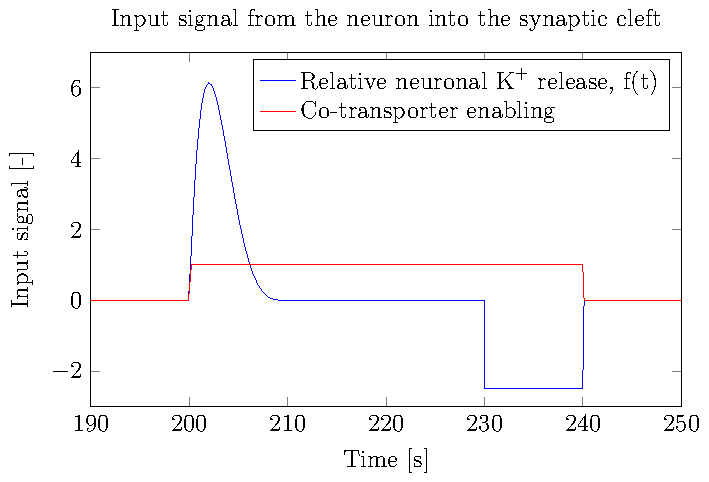
\includegraphics[width = 10cm]{pics/InputSignal.pdf}
	\caption{\textbf{The input signals used in the astrocyte model.} The \gls{K} efflux modelled by a beta distribution and buffered back afterwards (blue). The NKCC1 and KCC1 co-transporters are enabled when the neuronal ion release and spatial buffering is applied, modelled by a block function (red).  }
	\label{fig:InputSignal}
\end{figure}
% 
%
\subsubsection{Scaling}
The flux equations used in the AC model are based on the model of \citet{Ostby2009}. Their intention was to look at the volume changes of the AC and SC, therefore the volumes of both are variables in this model and all fluxes are scaled by a volume-surface ratio ($R_k$ and $R_s$, see Equations \ref{eq:R_k} and \ref{eq:R_tot}, respectively). It is assumed that the sum of the volumes of the AC and SC is a constant ($R_{tot}$). Due to osmotic pressure, the volume changes. We could show that the changes are comparatively small in our model and it would be justifiable to leave out the scaling factors. However, at the moment they are included because the given fluxes of \citet{Ostby2009} are scaled by the volume-surface ratio. It should be considered in future versions to eliminate the scaling factors by multiplying the fluxes with an adequate constant. 




\subsection{SMC and EC Model}
The SMC and EC model is based on the work of \citet{Koenigsberger2006}, see Figure~\ref{fig:SMCECmodel}. This model is extended by adding an inward-rectifier potassium (KIR) channel in the SMC ($ J_{KIR} $, \cite{Filosa2004}) in order to create a connection between the Astrocyte model and the SMC and EC model. \\%A conservation of \gls{K} was added in the SMC and EC model  for the PVS and SMC.\\

The input signal for this model is the \gls{K} concentration in the PVS which is increased by the efflux of astrocytic potassium after neuronal activity. 
\begin{figure}[h!]
  \centering
  \def\svgwidth{450pt} %400pt
  \scriptsize
  \import{pics/}{SMCECmodel3.pdf_tex}
  \caption{\textbf{Illustration of the SMC and EC model.} All modelled fluxes are pictured, note that the indices (k - Astrocyte (AC), s - Synaptic Cleft (SC), p - Perivascular Space (PVS)) are left out for clarity reasons.}
\label{fig:SMCECmodel}
\end{figure}

The raise in \gls{K} in the PVS activates the KIR channel on the SMC, causing them to open extruding more potassium into the PVS. This efflux of \gls{K} hyperpolarizes the SMC membrane and causing the voltage-operated \gls{Ca} channels to close, preventing the influx of \gls{Ca} into the SMC cytosol.\\

The cytosolic \gls{Ca} concentrations in the SMC and EC and that in the sacroplasmatic reticulum (SR) and endoplasmatic reticulum (ER), respectively, are described by a set of differential equations. In- and effluxes  of \gls{K} are given by the following ion channel and pumps: $ J_{KIR} $, $ J_{NaK} $ and $ J_{K} $. \gls{Ca} leaves the SR via the channels: $ J_{CICR} $, $ J_{IP_3} $ and $ J_{SR\_leak} $ and enters it by $ J_{SR\_upt} $. The in- and efflux of \gls{Ca} are modelled with $ J_{extr} $, $ J_{VOCC} $, $ J_{stretch} $ and $ J_{NaCa} $. Note that these fluxes link the cytosol with the extracellular matrix. Here again, a chloride pump is included, $ J_{Cl} $, to return to the resting membrane potential.\\

Physiologically, ECs and SMCs are connected by gap junctions that allow an intercellular exchange of molecules and voltage.  \citet{Koenigsberger2006} include the coupling factors $J_{Ca^{2+}-cpl}^{EC-SMC}$, $V_{cpl}^{EC-SMC}$ and $J_{IP_{3}-cpl}^{EC-SMC}$ for \gls{Ca}, voltage and IP$ _3 $ coupling, respectively. The strength of the coupling can be changed in the code with the variable $ CASE $.\\

Inositol triphosphate (\gls{IP3}) is an important messenger molecule. It's production, in the endothelium, is triggered by agonist binding onto membrane receptors. IP$_3$ mediates the $ J_{IP_3} $ channel, situated between the reticulum and cytosol. 
The production rate of IP3 is a constant over time and can be changed by altering the variable  $ J_{PLC}$ within the mathematical model .\\

Note that the model of \citet{Koenigsberger2006} already includes \gls{Ca}-buffering in the SMC and EC.







%\todo[inline]{What is the expected PLC agonist concentration in the EC?}
%\begin{itemize}
%\item based on \cite{Koenigsberger2006} with a KIR channel added
%\item \todo[inline]{rho as a buffering factor should be added (equation from \cite{Gonzalez1994})}
%\item coupling between EC and SMC included (voltage, Ca, IP3)
%\item \todo[inline]{include stretch activated channels}
%\item the only link between AC model and this model is the potassium efflux through the KIR channel  
%\item \todo[inline]{Potassium conservation of mass equation needs to be included}
%\item Do the NaK pump and the Ki channel lead into the PVS ? (at the moment into nowhere)
%\end{itemize}



%\todo[inline]{Tim's question: Should Ca coupling be included in the membrane potential equation? at the moment there is a voltage coupling, but we want to include also the Ca coupling in the membrane potential equation}

\subsection{Contraction and Mechanical Model}

\subsubsection{Contraction Model}
The contraction and mechanical part of the model is based on the model of \citet{Hai1989}, which describes the formation of cross bridges between the myosin and actin filaments (Figure~\ref{fig:MechModell}). This is coupled with a Kelvin-Voigt model that is used to describe the visco-elastic behaviour of the arterial wall (Figure~\ref{fig:KelvinVoigt}).\\
\begin{figure}[h!]
  \centering
  \def\svgwidth{450pt} %400pt
  \footnotesize
  \import{pics/}{MechanicalModel.pdf_tex}
  \caption{\textbf{Illustration of the contraction model within the smooth muscle cell. }}
\label{fig:MechModell}
\end{figure}

The \gls{Ca} concentration in the SMC is the input signal for the cross bridge model of \citet{Hai1989}. The model uses four possible states for the formation of myosin: free nonphosphorylated cross bridges (M), free phosphorylated cross bridges (Mp), attached phosphorylated cross bridges (AMp) and attached dephosphorylated latch bridges (AM). The dynamics of the fraction of myosin in a particular state is given by four differential equations.\\

The active stress of the SMC is directly proportional to the fraction of attached cross bridges (AM and AMp). Using this model the relation between the cytosolic \gls{Ca} concentration and the active stress of the SMC can be derived.\\

\subsubsection{Mechanical Model}
The fraction of attached myosin cross bridges is the input signal for the visco-elastic mechanical model (Kelvin Voigt, Figure~\ref{fig:KelvinVoigt})  which describes the changes in radius over time. The pressure inside the vessel wall is taken as a constant and the circumferential stress is calculated using the Laplacian law. 


\begin{figure}[h!]
  \centering
  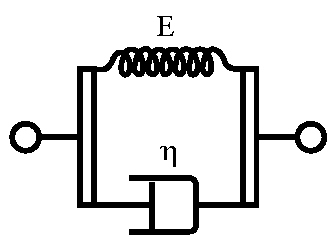
\includegraphics[width = 5 cm]{pics/Kelvin_Voigt_diagram.pdf}
  \caption{\textbf{Schematic overview of a Kelvin Voigt model.}}
  \label{fig:KelvinVoigt}
\end{figure}

The Young's modulus and initial radius of the vessel wall is divided into an active and a passive part and is a function of the attached myosin cross-bridges. The active and passive Young's modulus are based and fitted on experimental data of \citet{Gore} which is shown in Figure~\ref{fig:LinearisationRadius}. 

\begin{figure}[h!]
  \centering
  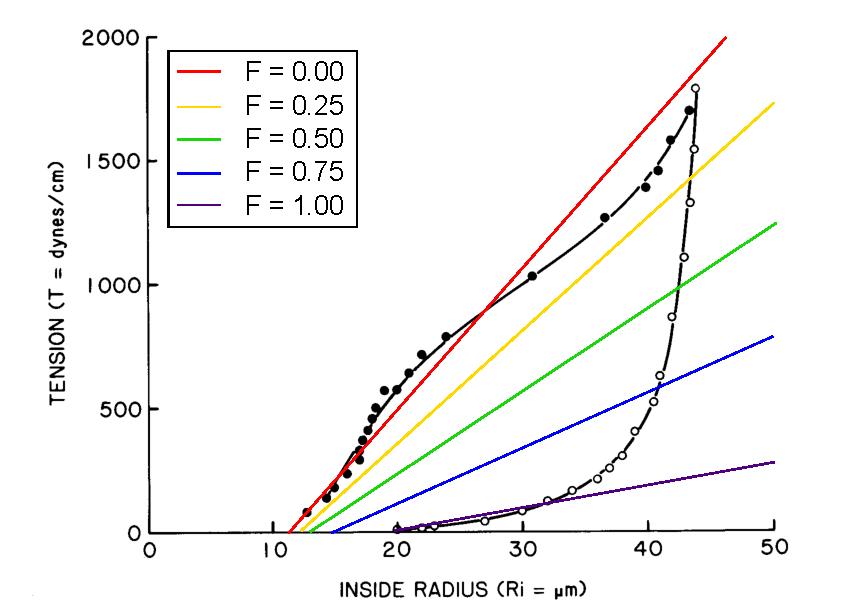
\includegraphics[width = 12 cm]{pics/LinearisationRadius.pdf}
  \caption{\textbf{Linearisation for the Young's modulus and initial radius on the data of \citet{Gore} for different values of F.}}
  \label{fig:LinearisationRadius}
\end{figure}

Figure~\ref{fig:LinearisationRadius} shows that the initial radius ($R_0$) decreases when the fraction of attached myosin cross bridges (F) are increased (the intersection with the x-axis). The figure also shows that the Young's modulus, represented by the slope of the lines in the tension-strain graph, increases when F increases. The linearisations of the Young's modulus can be described by:
\begin{equation} \label{eq:Fbalans4}
T=\frac{\Delta T}{\Delta R}(R-R_0)~,
\end{equation}
where $T$ is the tension of the vessel and $\frac{\Delta T}{\Delta R}$ is the slope of the linearisations in Figure~\ref{fig:LinearisationRadius}. \\

%Gore and Davis et al.\\
\newpage
\subsection{Merging of All Models}

The Astrocyte model and the \gls{SMC} and \gls{EC} model are linked by the SC and the \gls{PVS}. The \gls{K} input signal of the neuron is pumped into the \gls{SC} and taken up afterwards by the AC. The most important ion pumps and channels in this process are the \gls{K} channels in the neuron which releases the \gls{K} input,  the \gls{Na}/\gls{K} pump and \gls{K} channel in the \gls{AC} which pump the released \gls{K} into the AC.
The result of this is an efflux of \gls{K} at the end feet of the astrocyte using the BK-channel. Consequently, the membrane voltage of the astrocyte re-polarizes and the \gls{K} concentration in the PVS increases. This increased \gls{K} concentration activates the KIR channel in the \gls{SMC} and start to pump out more \gls{K} from the \gls{SMC} into the \gls{PVS}. The increased efflux of \gls{K} hyperpolarises the \gls{SMC} membrane voltage and as a result of that the VOCC closes and prevents the influx of \gls{Ca} into the \gls{SMC}.
Summarising, the neuronal input signal leads to a decrease of \gls{Ca} influx by the VOCC channels and therefore a decrease of the intracellular \gls{Ca} concentration. This leads to a decreased fraction of attached myosin bridges in the \citet{Hai1989} model, resulting in vessel dilation in the visco-elastic mechanical model. An overview of the whole model is shown in Figure~\ref{Overview}.

\begin{figure}[h!]
  \centering
  \def\svgwidth{450pt}
  \scriptsize 
  \import{pics/}{All_models_1pt1.pdf_tex}
  \caption{\textbf{All Models.}}
\label{Overview}
\end{figure}






%\begin{itemize}
%%\item What is the real relationship between the Ca concentration and the radius? - more references needed!
%%\item At the moment: Ca input of SMC, cross-bridge model of \citet{HaiMurphy}, Kelvin-Voigt model for elastic response of the arterial wall (assuming Laplace-law), change in radius 
%\end{itemize}


\section{Equations}

\subsection{Astrocyte Model}

\subsubsection{Scaling}
%
The  \gls{AC}  volume-area ratio (in $m$):
\begin{equation} \label{eq:R_k}
\dfrac{\mathrm{d}R_k}{\mathrm{d}t}= L_p \left( Na_k+K_k+Cl_k+HCO_{3_k}-Na_s-K_s-Cl_s-HCO_{3_{s}}+\frac{X_k}{R_k}\right)
\end{equation}
%
The \gls{SC} volume-surface ratio  (in $m$):
\begin{equation} \label{eq:R_tot}
R_s = R_{tot} - R_k  
\end{equation}
%
\begin{table}[h!]
\centering
\begin{tabular}{| p{0.09\linewidth} | >{\footnotesize} p{0.6\linewidth} | >{\footnotesize} p{0.17\linewidth} | >{\footnotesize} p{0.02\linewidth} |}
\arrayrulecolor{lightgrey}\hline
$L_p$ 			& The total water permeability per unit area of the astrocyte 			& 2.1e-9 \mperuMs &  \cite{Ostby2009}  \\
$X_k$			& Number of negatively charged impermeable ions trapped within the astrocyte divided by the astrocyte membrane area								& 12.41e-3 \uMm & \cite{Ostby2009}  \\
$R_{tot}$ 		& Total volume surface ratio AC+SC   		& 8.79e-8 \m & \cite{Ostby2009}  \\
\hline
\end{tabular}
\end{table}
\newpage
\subsubsection{Input Signal} \label{sec:InputSignal}
%
The neuronal \gls{K} input signal (-):\\
%
For $ t<t_0$ and $t>t_3$:
\begin{equation}
f(t)=0
\end{equation}
%
For $ t_0 \leq t \leq t_1$:
\begin{equation}
f(t)=F_{input} \dfrac{(\alpha+\beta-1)!}{(\alpha-1)!(\beta-1)!} \left( \dfrac{1-(t-t_0)}{\Delta t}\right) ^{\beta -1} \left( \dfrac{t-t_0}{\Delta t}\right) ^{\alpha -1} 
\end{equation}
%
For $ t_1 \leq t \leq t_2$:
\begin{equation}
f(t)=0
\end{equation}
%
For $ t_2 \leq t \leq t_3$:
\begin{equation}
f(t)=-F_{input}
\end{equation}
%
\paragraph{$\rho$ input signal}
The smooth pulse function $\rho$
\begin{equation}
\rho(t) = \frac{Amp - base}{2}\times\left(1+\mathrm{tanh}\left(\frac{t-t_0}{\theta_L}\right)\right)+base+\frac{Amp-base}{2}\times\left(1+\mathrm{tanh}\left(\frac{t-t_2}{\theta_R}\right)\right)+base-Amp                      
\end{equation}
%
\begin{table}[h!]
\centering
\begin{tabular}{| p{0.09\linewidth} | >{\footnotesize} p{0.6\linewidth} | >{\footnotesize} p{0.17\linewidth} | >{\footnotesize} p{0.02\linewidth} |}
\arrayrulecolor{lightgrey}\hline
$t_0$ 			& Start of neuronal pulse	& 200 s &  ME  \\
$t_1$ 			& End of neuronal pulse	& 210 s &  ME  \\
$t_2$ 			& Start of back-buffering	& 230 s &  ME  \\
$t_3$ 			& End of back-buffering	& 240 s &  ME  \\
$F_{input}$ 	& Amplitude scaling factor 	& 2.5 	&  ME  \\
$\alpha$ 		& Beta-distribution constant	& 2 	&  ME  \\
$\beta$ 		& Beta-distribution constant	& 5 	&  ME  \\
$\Delta t$ 		& Time-scaling factor	& 10 s	&  ME  \\
$Amp$           & Amplitude of smooth pulse function & 0.7 & ME\\
$base$          & Baseline of smooth pulse function & 0.1 & ME\\
$\theta_L$      & Left ramp of smooth pulse function & 1 & ME\\
$\theta_R$      & Left ramp of smooth pulse function & 1 & ME\\
   
\hline
\end{tabular}
\end{table}

% 
\subsubsection{Conservation Equations}
\paragraph{Synaptic Cleft}~\\
%
\gls{K} concentration in the \gls{SC} (times the \gls{SC} volume-area ratio $R_s$; in \uMm):
\begin{equation} \label{eq:KEx}
\dfrac{\mathrm{d}N_{K_s}}{\mathrm{d}t}= k_C f(t) -\dfrac{\mathrm{d}N_{K_k}}{\mathrm{d}t} - J_{BK_k} 
\end{equation}
%
\gls{Na} concentration in the \gls{SC}  (times the \gls{SC} volume-area ratio $R_s$; in \uMm):
\begin{equation} \label{eq:NaEx}
\dfrac{\mathrm{d}N_{Na_s}}{\mathrm{d}t}= - k_C f(t) -\dfrac{\mathrm{d}N_{Na_k}}{\mathrm{d}t}
\end{equation}
%
\gls{HCO3} concentration in the SC  (times the \gls{SC} volume-area ratio $R_s$; in \uMm):
\begin{equation} \label{eq:HCOEx}
\dfrac{\mathrm{d}N_{HCO_{3_{s}}}}{\mathrm{d}t}=-\dfrac{\mathrm{d}N_{HCO_{3_{k}}}}{\mathrm{d}t}
\end{equation}
\begin{table}[h!]
\centering
\begin{tabular}{| p{0.09\linewidth} | >{\footnotesize} p{0.6\linewidth} | >{\footnotesize} p{0.17\linewidth} | >{\footnotesize} p{0.02\linewidth} |}
\arrayrulecolor{lightgrey}\hline
$ k_C $  & Input scaling parameter & 7.35e-5 \muMps & \cite{Ostby2009} \\
\hline
\end{tabular}
\end{table}

\paragraph{Astrocyte}~\\
%
\gls{K} concentration in the AC  (times the AC volume-area ratio $R_k$; in \uMm):
\begin{equation} \label{eq:KInt}
\dfrac{\mathrm{d}N_{K_k}}{\mathrm{d}t}=- J_{K_k} + 2 J_{NaK_{k}} + J_{NKCC1_{k}} +  J_{KCC1_{k}}
- J_{BK_k}  
\end{equation}
%
\gls{Na} concentration in the AC  (times the AC volume-area ratio $R_k$; in \uMm):
\begin{equation} \label{eq:NaInt}
\dfrac{\mathrm{d}N_{Na_k}}{\mathrm{d}t}=-J_{Na_k} - 3 J_{NaK_{k}} + J_{NKCC1_{k}} +  J_{NBC_{k}}
\end{equation}
%
\gls{HCO3} concentration in the AC  (times the AC volume-area ratio $R_k$; in \uMm):
\begin{equation} \label{eq:HCOInt}
\dfrac{\mathrm{d}N_{HCO_{3_k}}}{\mathrm{d}t}= 2 J_{NBC_{k}} 
\end{equation}
%
\gls{Cl} concentration in the AC  (times the AC volume-area ratio $R_k$; in \uMm):
\begin{equation} \label{eq:ClInt}
\dfrac{\mathrm{d}N_{Cl_k}}{\mathrm{d}t}= \dfrac{\mathrm{d}N_{Na_k}}{\mathrm{d}t} + \dfrac{\mathrm{d}N_{K_k}}{\mathrm{d}t} - \dfrac{\mathrm{d}N_{HCO_{3_{k}}}}{\mathrm{d}t}
\end{equation}
%
\gls{Ca} concentration in the astrocytic cytosol:
\begin{equation} \label{eq:ckInt}
\dfrac{\mathrm{d}c_k}{\mathrm{d}t}= B_{\mathrm{cyt}}(J_{\mathrm{IP_3}}-J_{\mathrm{pump}}+J_{\mathrm{ER_leak}})
\end{equation}
%
\gls{Ca} concentration in the astrocytic \gls{ER}:
\begin{equation} \label{eq:skInt}
\dfrac{\mathrm{d}s_k}{\mathrm{d}t}= \frac{1}{VR_{\mathrm{ER_cyt}}}(\frac{dc_k}{dt})
\end{equation}
%
The inactivation variable for \gls{IP3}:
\begin{equation} \label{eq:hkInt}
\dfrac{\mathrm{d}h_k}{\mathrm{d}t}= k_{\mathrm{on}}[K_{\mathrm{inh}}-(c_k+K_{\mathrm{inh}})h_k]
\end{equation}
%
The \gls{IP3} concentration:
\begin{equation} \label{eq:ikInt}
\dfrac{\mathrm{d}i_k}{\mathrm{d}t}= r_hG-k_{\mathrm{deg}}i_k
\end{equation}
%
The EET concentration:
\begin{equation} \label{eq:eetkInt}
\dfrac{\mathrm{d}eetk_k}{\mathrm{d}t}= V_{\mathrm{eet}}(c_k-c_{\mathrm{k,min}})-k_{\mathrm{eet}}eet_k
\end{equation}
%
Open probability of the BK channel (\pers):
\begin{equation} \label{eq:dwkdt}
\frac{\mathrm{d}w_{k}}{\mathrm{d}t} = \phi_{w} \left(w_{\infty}-w_{k} \right) 
\end{equation}
%
\begin{table}[h!]
	\centering
	\begin{tabular}{| p{0.09\linewidth} | >{\footnotesize} p{0.6\linewidth} | >{\footnotesize} p{0.17\linewidth} | >{\footnotesize} p{0.02\linewidth} |}
		\arrayrulecolor{lightgrey}\hline
		$ VR_{\mathrm{ER_{\mathrm{cyt}}}} $  & Volume ratio of the \gls{ER} to the cytosol in the astrocyte  & 0.185 [-] & \cite{} \\
		$k_{\mathrm{on}} $         & Rate of \gls{Ca} binding to the \gls{IP3}R  & 2 [\uMps] &  \cite{} \\
		$K_{\mathrm{inh}}$          & Dissociation rate of $k_{\mathrm{on}}$  & 0.1[\uM] & \cite{} \\
		$r_h$                      & Maximum rate of \gls{IP3} production in the astrocyte  &  4.8 [\uM] & \cite{} \\
		$k_{\mathrm{deg}}$          & Rate constant for \gls{IP3} degradation  &  1.25 [\pers] & \cite{} \\
		$V_{\mathrm{eet}} $        & Rate constant for EET production   & 72 [\uM] & \cite{} \\
		$k_{\mathrm{eet}}$         & Rate constant for EET degradation  & 7.2 [\uM] & \cite{} \\
		$c_{\mathrm{k,min}}$       & Minimum \gls{Ca} concentration required for EET production & 0.1 [uM] & \cite{} \\			
		\hline
	\end{tabular}
\end{table}
%
\paragraph{Perivascular Space}~\\
\gls{K} concentration in the PVS  (in \uM):
\begin{equation} \label{eq:K_p}
\dfrac{\mathrm{d}K_{p}}{\mathrm{d}t}= \frac{J_{BK_k}}{R_k VR_{pa}} + \frac{J_{KIR_i}}{ VR_{ps}}
\end{equation}
%
\begin{table}[h!]
\centering
\begin{tabular}{| p{0.09\linewidth} | >{\footnotesize} p{0.6\linewidth} | >{\footnotesize} p{0.17\linewidth} | >{\footnotesize} p{0.02\linewidth} |}
\arrayrulecolor{lightgrey}\hline
$ VR_{pa} $  & Volume ratio of PVS to AC & 0.001 [-] & \cite{LoesEvert} \\
$ VR_{ps} $  & Volume ratio of PVS to SMC & 0.001 [-] & \cite{LoesEvert} \\
\hline
\end{tabular}
\end{table}

\subsubsection{Fluxes}~\\
%
\gls{K} flux (times the AC volume-area ratio $R_k$; in \uMmps): 
\begin{equation} \label{eq:J_K}
J_{K_k}=\frac{g_{K_{k}}}{F}(v_k - E_{K_k}) C_{correction}
\end{equation}
%
\gls{Na} flux (times the AC volume-area ratio $R_k$; in \uMmps):
\begin{equation} \label{eq:J_Na}
J_{Na_k}=\frac{g_{Na_{k}}}{F}(v_k - E_{Na_k}) C_{correction}
\end{equation}
%
\gls{Na} and \gls{HCO3} flux through the NBC channel  (times the AC volume-area ratio $R_k$; in \uMmps): 
\begin{equation} \label{eq:J_NBC}
J_{NBC_k}=\frac{g_{NBC_k}}{F}\left(  v_k -E_{NBC_k}  \right) C_{correction}
\end{equation}
%
\gls{Cl} and \gls{K} flux through the KCC1 channel  (times the AC volume-area ratio $R_k$; in \uMmps): 
\begin{equation} \label{eq:J_KCC1}
J_{KCC1_k}=C_{input}\frac{g_{KCC1_k}}{F}\frac{RT}{F}ln \left(\frac{K_s Cl_s }{K_k Cl_k}\right) C_{correction}
\end{equation}
%
\gls{Na}, \gls{K} and \gls{Cl} flux through the NKCC1 channel   (times the AC volume-area ratio $R_k$; in \uMmps): 
\begin{equation} \label{eq:J_NKCC1}
J_{NKCC1_k}=C_{input}\frac{g_{NKCC1_k}}{F}\frac{RT}{F}ln \left(\frac{Na_s K_s {Cl_s}^2}{Na_k K_k {Cl_k}^2}\right) C_{correction}
\end{equation}
%
Flux through the sodium potassium pump   (times the \gls{AC} volume-area ratio $R_k$; in \uMmps): 
\begin{equation} \label{eq:J_NaK_s}
J_{NaK_{k}}=J_{NaK_{max}}\frac{{Na_k}^{1.5}}{{Na_k}^{1.5}+{K_{Na_k}}^{1.5}}\frac{K_s}{K_s+K_{K_s}}
\end{equation}
%
\gls{K} flux through the BK channel  (times the \gls{AC} volume-area ratio $R_k$; in \uMmps): 
\begin{equation} \label{eq:J_BK}
J_{BK_k}=\frac{g_{BK_k}}{F}w_k\left( v_k-E_{BK_k} \right) C_{correction}
\end{equation}
%
\gls{Ca} flux from the ER to the cytosol in the astrocyte through \gls{IP3} Receptors (\gls{IP3}R) by \gls{IP3}: 
\begin{equation} \label{eq:J_ip3}
J_{\mathrm{IP3}}=J_{\mathrm{max}}[(\frac{i_k}{i_k+K_i})(\frac{c_k}{c_k+K_{\mathrm{act}}})h_k]^3\times [1-\frac{c_k}{s_k}] 
\end{equation}
%
The leakage \gls{Ca}  flux from the \gls{ER} to the cytosol in the astrocyte:
\begin{equation} \label{eq:J_ER_leak}
J_{\mathrm{ER_leak}} = P_L(1-\frac{c_k}{s_k})
\end{equation}	
%
The ATP dependent \gls{Ca}  pump flux from the cytoplasm to the ER in the astrocyte:
\begin{equation} \label{eq:J_pump}
J_{\mathrm{pump}} = V_{\mathrm{max}}\frac{c_k^2}{c_k^2+k_pump^2}
\end{equation}
%
%
%
\begin{table}[h!]
\centering
\begin{tabular}{| p{0.09\linewidth} | >{\footnotesize} p{0.6\linewidth} | >{\footnotesize} p{0.17\linewidth} | >{\footnotesize} p{0.02\linewidth} |}
\arrayrulecolor{lightgrey}\hline	
$F$ 			& Faradays constant														& 9.649e4 \Cmol 	& \\
$R_g$ 			& Gas constant 															& 8.315 \JmolK		& \\
$T$ 	    	& Temperature 															& 300 \Kelvin		& \\
$g_{K_{k}}$ 	& Specific ion conductance of potassium 								& 40 \perOhmm 		& \cite{Ostby2009}  \\
$g_{Na_k}$ 		& Specific ion conductance of sodium 									& 1.314  \perOhmm 	& \cite{Ostby2009}  \\
$g_{NBC_k}$ 	& Specific ion conductance of the NBC cotransporter						& 7.57e-1 \perOhmm 	& \cite{Ostby2009}  \\
$g_{KCC1_k}$ 	& Specific ion conductance of the KCC1 cotransporter					& 1e-2 \perOhmm 	& \cite{Ostby2009}  \\
$g_{NKCC1_k}$ 	& Specific ion conductance of the NKCC1 cotransporter	 				& 5.54e-2 \perOhmm 	& \cite{Ostby2009}  \\
$J_{NaK_{max}}$ & The maximum flux through the NaKATPase pump							& 1.42e-3 \uMms 	& \cite{Ostby2009}  \\
$g_{BK_k}$ 		& Specific ion conductance of the BK channel							& 1.16     \perOhmm & \cite{LoesEvert}  \\
$C_{correction}$  & correction factor                                                   & 10e3 [-]        & \cite{LoesEvert} \\
$C_{input}$     & Block function to switch the channel on and off                       & 0 ; 1 [-]         & \cite{LoesEvert} \\
$J_{max}$       & Maximum \gls{IP3} rate                                                & 2880 \uMps        & \cite{Farr2011} \\  
$K_I$           & Dissociation constant for \gls{IP3} binding to \gls{IP3}R             & 0.03 \uM          & \cite{Farr2011} \\ 
$K_{act}$       & Dissociation constant for \gls{Ca} binding to \gls{IP3}R              & 0.17 \uM          & \cite{Farr2011} \\ 
$P_L$           & Associated with the steady state \gls{Ca} balance                     & 5.2 \uM           & \cite{Farr2011} \\ 
$V_{max}$       & Maximal pumping rate of the \gls{Ca} pump                             & 20 \uMps          & \cite{Farr2011} \\ 
$k_{pump}$      & Dissociation constant of the \gls{Ca} pump                            & 0.24 \uM          & \cite{Farr2011} \\ 
\hline
\end{tabular}
\end{table}



\newpage
\subsubsection{Additional Equations}
\paragraph{Synaptic Cleft}~\\
%
\gls{Cl} concentration  (times the SC volume-area ratio $R_s$; in \uMm): 
\begin{equation} \label{eq:ClEx}
N_{Cl_s}= N_{Na_s}+N_{K_s}-N_{ HCO_{3_s}}
\end{equation}

\paragraph{Astrocyte}~\\
%
Membrane voltage of the \gls{AC} (mV):
\begin{equation} \label{eq:v_k}
v_k=\frac{g_{Na_k}E_{Na_k}+g_{K_k}E_{K_k}+g_{Cl_k}E_{Cl_k}+g_{NBC_k}E_{NBC_k} + g_{BK_k}w_kE_{BK_k} -J_{NaK_k}F C_{correction} }{ g_{Na_k}+g_{K_k}+g_{Cl_k}+g_{NBC_k}+g_{BK_k}w_k }
\end{equation}
%
Nernst potential for the potassium channel (in mV):
\begin{equation} \label{eq:E_K}
E_{K_k}=\frac{R_gT}{z_K F}ln\left( \frac{K_s}{K_k}\right) 
\end{equation}
%
Nernst potential for the sodium channel (in mV):
\begin{equation} \label{eq:E_Na}
E_{Na_k}=\frac{R_gT}{z_{Na} F}ln\left( \frac{Na_s}{Na_k}\right) 
\end{equation}
%
Nernst potential for the chloride channel (in mV):
\begin{equation} \label{eq:E_Cl}
E_{Cl_k}=\frac{R_gT}{z_{Cl} F}ln\left( \frac{Cl_s}{Cl_k}\right) 
\end{equation}
%
Nernst potential for the NBC channel (in mV):
\begin{equation} \label{eq:E_NBC}
E_{NBC_k}=\frac{R_gT}{z_{NBC} F}ln\left( \frac{Na_s {HCO_{3_s}}^2}{Na_k {HCO_{3_k}}^2}\right) 
\end{equation}
Nernst potential for the BK channel (in mV):
\begin{equation} \label{eq:E_BK}
E_{BK_k}=\frac{R_gT}{z_K F}ln\left( \frac{K_p}{K_k}\right) 
\end{equation}
The Calcium buffering parameter in the astrocytic cytosol (-)
 \begin{equation} \label{eq:B_cyt}
 	B_{cyt}=\left(1+BK_{end}+ \frac{K_{ex}B_{ex}}{(K_{ex}+c_k)^2}\right)^{-1} 
 \end{equation}
The ratio of active to total G-protein (-)
\begin{equation} \label{eq:G}
   G=\frac{\rho+\delta}{K_g+\rho+\delta}
\end{equation}
Equilibrium state BK-channel (-):
\begin{equation} \label{eq:winf}
w_{\infty}=0.5 \left(1+\mathrm{tanh}\left(\frac{v_{k}+(eet_{\mathrm{shift}}eet_k)-v_{3} }{v_{4}} \right)  \right) 
\end{equation}
%
The time constant associated with the opening of BK channels	 (in \pers):
\begin{equation} \label{eq:phin}
\phi_{w}=\psi_{w}\mathrm{cosh}\left( \frac{v_{k}-v_{3}}{2v_{4}}\right) 
\end{equation}
\gls{Ca} dependent shift of the opening of the BK-channels
\begin{equation} \label{eq:v_3}
v_{3}=\frac{v_5}{2}\mathrm{tanh}\left( \frac{c_k-Ca_3}{Ca_4}\right)+v_6 
\end{equation}

\begin{table}[h!]
\centering
\begin{tabular}{| p{0.09\linewidth} | >{\footnotesize} p{0.6\linewidth} | >{\footnotesize} p{0.17\linewidth} | >{\footnotesize} p{0.02\linewidth} |}
\arrayrulecolor{lightgrey}\hline
$g_{Cl_k}$ 		& Specific ion conductance of chloride 									& 8.797e-1 [\perOhmm] & \cite{Ostby2009}  \\
$z_K$			& Valence of a potassium ion										& 1  [-] & \\ 
$z_Na$			& Valence of a sodium ion											& 1  [-] & \\ 
$z_Cl$			& Valence of a chloride ion											& -1 [-] & \\ 
$z_{NBC}$ 		& Effective valence of the NBC cotransporter complex 				& -1 [-] & \\
$BK_{end}$      & Cytosolic endogenous buffer constant                              & 40 [-] & \cite{LoesEvert} \\
$K_{ex}$        & Cytosolic exogenous buffer dissociation constant                  & 0.26 [\uM] & \cite{LoesEvert} \\
$B_{ex}$        & Concentration of cytosolic exogenous buffer                       & 11.35 [\uM] & \cite{LoesEvert} \\
$\delta$        & Ratio of the activities of the bound and unbound receptors        & 1.235e-3 [-] & \cite{Farr2011}\\
$K_G$           & The G-protein dissociation constant                               & 8.82  [uM] & \cite{Farr2011}\\
$v_{4}$			& A measure of the spread of the distribution of the open probability of the BK channel	& 14.5e-3 [\Volt]   &  \cite{Gonzalez1994}  
\\
$v_{5}$			& Determines the range of the shift of $n_{\inf}$ as calcium varies    		& 8e-3 [\Volt]  & \cite{Farr2011}  \\
$v_{6}$			& The voltage associated with the opening of half the population		& -15e-3 [\Volt]  & \cite{Farr2011}  \\
$ \psi_{w}$    	& A characteristic time for the open probability of the BK channel		& 2.664 [$s^{-1}$] & \cite{Gonzalez1994} \\

\hline
\end{tabular}
\end{table}


\newpage
\subsection{SMC and EC Model}


\subsubsection{Conservation Equations}
\paragraph{Smooth Muscle Cell}~\\
%
The cytosolic [\gls{Ca}] in the \gls{SMC} (in \uM):
\begin{equation}\label{eq:ci}
\begin{split}
\dfrac{\mathrm{d}\CaConsc}{\mathrm{d}t} = J_{IP_{3i}} - J_{SR_{uptake_{i}}} + J_{CICR_{i}} - J_{extrusion_{i}} +  J_{SR_{leak_{i}}}\dots \\
 - J_{VOCC_{i}} + J_{Na/Ca_{i}}  + 0.1J_{stretch_{i}} + J_{Ca^{2+}-coupling_{i}}^{SMC-EC}
\end{split} 
\end{equation}
%
The [Ca$^{2+}$] in the \gls{SR} of the \gls{SMC} (in \uM):
\begin{equation} \label{eq:si}
\dfrac{\mathrm{d}\CaConse}{\mathrm{d}t} =  J_{SR_{uptake_{i}}} - J_{CICR_{i}} - J_{SR_{leak_{i}}}
\end{equation}
%
The membrane potential of the \gls{SMC} (in \mV):
\begin{equation} \label{eq:vi}
\begin{split}
\dfrac{\mathrm{d}v_{i}}{\mathrm{d}t} = \gamma_{i}( -J_{Na/K_{i}} - J_{Cl_{i}} - 2J_{VOCC_{i}}- J_{Na/Ca_{i}} - J_{K_{i}} \dots \\
- J_{stretch_{i}} - J_{KIR_{i}} ) +V^{SMC-EC}_{coupling_{i}}
\end{split}
\end{equation}
%
The open state probability of calcium-activated potassium channels (dimensionless):
\begin{equation} \label{eq:dwidt}
\dfrac{\mathrm{d}w_{i}}{\mathrm{d}t} =  \lambda_{i} \left( K_{act_{i}} - w_{i} \right)
\end{equation}
%
The \gls{IP3} concentration om the \gls{SMC} (in \uM):
\begin{equation} \label{eq:dIidt}
\dfrac{\mathrm{d}\IP _{i}}{\mathrm{d}t} = J^{SMC-EC}_{IP_{3}-coupling_{i}} - J_{degrad_{i}}
\end{equation}
%
The \gls{K} concentration in the \gls{SMC} (in \uM):
\begin{equation} \label{eq:dkidt}
\dfrac{\mathrm{d} [K^+_{i}]}{\mathrm{d}t}  = J_{Na/K_{i}}  - J_{KIR_{i}} - J_{K_{i}}
\end{equation}

\begin{table}[h!]
\centering
\begin{tabular}{| p{0.09\linewidth} | >{\footnotesize} p{0.6\linewidth} | >{\footnotesize} p{0.17\linewidth} | >{\footnotesize} p{0.02\linewidth} |}
\arrayrulecolor{lightgrey}\hline
$\gamma_{i}$				& The change in membrane potential by a scaling factor					& 1970 \mVpuM	& \cite{Koenigsberger2006} \\
$\lambda_{i} $				& The rate constant for opening											& 45.0 \pers 	& \cite{Koenigsberger2006} \\
%$\CaConsc$      		& The cytololic [Ca$^{2+}$] in the SMC    								& var. \uM		& - \\
\hline
\end{tabular}
\label{tab:dcidt}
\end{table}

\paragraph{Endothelial Cell}~\\
%
The cytosolic \gls{Ca} concentration in the \gls{EC} (in \uM):
\begin{equation} \label{eq:cj}
\begin{split}
\dfrac{\mathrm{d}\CaConec}{\mathrm{d}t} = J_{IP_{3j}} - J_{ER_{uptake_{j}}} + J_{CICR_{j}} - J_{extrusion_{j}}\dots \\
 + J_{ER_{leak_{j}}} + J_{cation_{j}} + J_{0_{j}} + J_{stretch_{j}} - J_{Ca^{2+}-coupling_{j}}^{SMC-EC}
\end{split}
\end{equation}
%
The \gls{Ca} concentration in the \gls{ER} in the \gls{EC} (in \uM): %copied from SMC
\begin{equation} \label{eq:sj}
\dfrac{\mathrm{d}\CaConee}{\mathrm{d}t} =  J_{SR_{uptake_{j}}} - J_{CICR_{j}} - J_{SR_{leak_{j}}}
\end{equation}
%
The membrane potential of the \gls{EC} (in \mV):
\begin{equation} \label{eq:dvjdt}
\dfrac{\mathrm{d}v_{j}}{\mathrm{d}t} =-\frac{1}{C_{m_{j}}} ( J_{K_{j}}+J_{R_{j}}) + V^{SMC-EC}_{coupling_{j}}
\end{equation}
%
The \gls{IP3} concentration of the \gls{EC} (in \uM):
\begin{equation} \label{eq:dIjdt}
\dfrac{\mathrm{d}\IP_{j}}{\mathrm{d}t} =  J_{agonist_{j}}- J_{degrad_{j}}  - J^{SMC-EC}_{IP_{3}-coupling_{j}}
\end{equation}

\begin{table}[h!]
\centering
\begin{tabular}{| p{0.09\linewidth} | >{\footnotesize} p{0.6\linewidth} | >{\footnotesize} p{0.17\linewidth} | >{\footnotesize} p{0.02\linewidth} |}
\arrayrulecolor{lightgrey}\hline
 $C_{m_{j}}$				& Membrane capacitance												& 25.8  \pF		& \cite{Koenigsberger2006} \\
 
\hline
\end{tabular}
\label{tab:CIP3j}
\end{table}
%\\

\subsubsection{Fluxes}
%
\paragraph{Smooth Muscle Cell}~\\
%
The release of calcium from IP$_{3}$ sensitive stores in the SMC (in \uMps):
\begin{equation} \label{eq:IP3i}
J_{IP_{3i}} = F_{i}\frac{\IP_{i}^{2}}{K_{ri}^{2}+\IP_{i}^{2}}
\end{equation}
%
\begin{table}[h!]
\centering
\begin{tabular}{| p{0.09\linewidth} | >{\footnotesize} p{0.6\linewidth} | >{\footnotesize} p{0.17\linewidth} | >{\footnotesize} p{0.02\linewidth} |}
\arrayrulecolor{lightgrey}\hline
 $F_{i}$      			& Maximal rate of activation-dependent calcium influx			& 0.23 \uMps				& \cite{Koenigsberger2006} \\
$K_{ri}$				& Half-saturation constant for agonist-dependent calcium entry	& 1 \uM					& \cite{Koenigsberger2006} \\
\hline
\end{tabular}
\label{tab:IP3i}
\end{table}
\\
%
\newpage The uptake of calcium into the sarcoplasmic reticulum (in \uMs):
\begin{equation} \label{eq:JSRuptakei}
J_{SR_{uptake_{i}}} = B_{i}\frac{\CaConsc^{2}}{c_{bi}^{2}+\CaConsc^{2}}
\end{equation}
%
\begin{table}[h!]
\centering
\begin{tabular}{| p{0.09\linewidth} | >{\footnotesize} p{0.6\linewidth} | >{\footnotesize} p{0.17\linewidth} | >{\footnotesize} p{0.02\linewidth} |}
\arrayrulecolor{lightgrey}\hline
$B_{i}$      			& SR uptake rate constant							& 2.025 \uMs				& \cite{Koenigsberger2006} \\
$c_{bi}$				& Half-point of the SR ATPase activation sigmoidal (oder Michaelis (Menten) constant) 	& 1.0 \uM					& \cite{Koenigsberger2006} \\
\hline
\end{tabular}
\label{tab:JSRuptakei}
\end{table}
\\
%
The calcium-induced calcium release (CICR; in \uMs):
\begin{equation} \label{eq:JCICRi}
J_{CICR_{i}} = C_{i}\frac{\CaConse^{2}}{s_{ci}^{2}+\CaConse^{2}}    \frac{\CaConsc^{4}}{c_{ci}^{4}+\CaConsc^{4}}
\end{equation}
%
\begin{table}[h!]
\centering
\begin{tabular}{| p{0.09\linewidth} | >{\footnotesize} p{0.6\linewidth} | >{\footnotesize} p{0.17\linewidth} | >{\footnotesize} p{0.02\linewidth} |}
\arrayrulecolor{lightgrey}\hline
$C_{i}$      			& CICR rate constant									& 55 \uMs		& \cite{Koenigsberger2006} \\
$s_{ci}$				& Half-point of the CICR Ca$^{2+}$ efflux sigmoidal			& 2.0 \uM		& \cite{Koenigsberger2006} \\
$c_{ci}$				& Half-point of the CICR activation sigmoidal			& 0.9 \uM		& \cite{Koenigsberger2006} \\
\hline
\end{tabular}
\label{tab:JCICRi}
\end{table}
\\
%
The calcium extrusion by Ca$^{2+}$-ATPase pumps (in \uMs):
\begin{equation} \label{eq:Jextrusioni}
J_{extrusion_{i}} = D_{i}\CaConsc   \left( 1+ \frac{v_{i}-v_{d}}{R_{di}}\right)
\end{equation}
%
\begin{table}[h!]
\centering
\begin{tabular}{| p{0.09\linewidth} | >{\footnotesize} p{0.6\linewidth} | >{\footnotesize} p{0.17\linewidth} | >{\footnotesize} p{0.02\linewidth} |}
\arrayrulecolor{lightgrey}\hline
$D_{i}$      			& Rate constant for Ca$^{2+}$ extrusion by the ATPase pump		 & 0.24	\pers			& \cite{Koenigsberger2005} \\
$v_{d}$					& Intercept of voltage dependence of extrusion ATPase			 & -100.0 \mV			& \cite{Koenigsberger2006} \\
$R_{di}$				& Slope of voltage dependence of extrusion ATPase.				 & 250.0 \mV			& \cite{Koenigsberger2006} \\
\hline
\end{tabular}
\label{tab:Jextrusioni}
\end{table}
\\
%
The leak current from the SR (in \uMs):
\begin{equation} \label{eq:JSRleaki}
J_{SR_{leak_{i}}} = L_{i}\CaConse
\end{equation}
\begin{table}[h!]
\centering
\begin{tabular}{| p{0.09\linewidth} | >{\footnotesize} p{0.6\linewidth} | >{\footnotesize} p{0.17\linewidth} | >{\footnotesize} p{0.02\linewidth} |}
\arrayrulecolor{lightgrey}\hline
$L_{i}$      			& Leak from SR rate constant						 & 0.025 \pers				& \cite{Koenigsberger2006} \\
\hline
\end{tabular}
\label{tab:Jleaki}
\end{table}
\\
%
\newpage
The calcium influx through VOCCs (in \uMs): 
\begin{equation} \label{eq:JVOCCi}
J_{VOCC_{i}} = G_{Cai} \frac{v_{i}-v_{Ca_{1i}}}     {1+ exp(-\left[ \left(  v_{i}-v_{Ca_{2i}}\right) /R_{Cai}      \right] )}
\end{equation}
\begin{table}[h!]
\centering
\begin{tabular}{| p{0.09\linewidth} | >{\footnotesize} p{0.57\linewidth} | >{\footnotesize} p{0.2\linewidth} | >{\footnotesize} p{0.02\linewidth} |}
\arrayrulecolor{lightgrey}\hline
$G_{Cai}$      	& Whole-cell conductance for VOCCs	 					& 1.29e-3  \uMpmVs					& \cite{Koenigsberger2006} \\
$v_{Ca_{1i}}$   & Reversal potential for VOCCs	 						& 100.0 \mV							& \cite{Koenigsberger2006} \\
$v_{Ca_{2i}}$  	& Half-point of the VOCC activation sigmoidal		 	& -24.0 \mV							& ME \\
$R_{Cai}$      	& Maximum slope of the VOCC	activation sigmoidal		& 8.5 \mV							& \cite{Koenigsberger2006} \\
\hline
\end{tabular}
\label{tab:JVOCCi}
\end{table}
\\
%
The flux of calcium exchanging with sodium in the Na$^{+}$Ca$^{2+}$ exchange (in \uMs): 
\begin{equation} \label{eq:JNaCai}
J_{Na/Ca_{i}} = G_{Na/Ca_{i}} \frac{\CaConsc}     {\CaConsc + c_{Na/Cai}} \left( v_{i}-v_{Na/Ca_{i}} \right)
\end{equation}
%
\begin{table}[h!]
\centering
\begin{tabular}{| p{0.09\linewidth} | >{\footnotesize} p{0.57\linewidth} | >{\footnotesize} p{0.2\linewidth} | >{\footnotesize} p{0.02\linewidth} |}
\arrayrulecolor{lightgrey}\hline
$G_{Na/Cai}$   	& Whole-cell conductance for Na$^{+}$/Ca$^{2+}$ exchange			 		 & 3.16e-3 \uMpmVs	& \cite{Koenigsberger2005} \\
$c_{Na/Cai}$   	& Half-point for activation of Na$^{+}$/Ca$^{2+}$ exchange by Ca$^{2+}$		 & 0.5 \uM			& \cite{Koenigsberger2006} \\
$v_{Na/Cai}$   	& Reversal potential for the Na$^{+}$/Ca$^{2+}$ exchanger					 & -30.0 \mV		& \cite{Koenigsberger2006} \\
\hline
\end{tabular}
\label{tab:JNaCai}
\end{table}
\\
%
The calcium flux through the stretch-activated channels in the SMC (in \uMs): 
\begin{equation} \label{eq:Jstretchi}
\begin{split}
J_{stretch_{i}}= \frac{G_{stretch}}{1+ exp\left(-\alpha_{stretch}  \left(  \frac{\Delta pR}{h} -\sigma_{0}   \right) \right)}  \left(  v_{i}-E_{SAC}   \right) 
\end{split}
\end{equation}
%
\begin{table}[h!]
\centering
\begin{tabular}{| p{0.09\linewidth} | >{\footnotesize} p{0.57\linewidth} | >{\footnotesize} p{0.2\linewidth} | >{\footnotesize} p{0.02\linewidth} |}
\arrayrulecolor{lightgrey}\hline
$G_{stretch}$      		& The whole cell conductance for SACs						& 6.1e-3 \uMpmVs	&\cite{Koenigsberger2006} \\
$\alpha_{stretch}$      & Slope of stress dependence of the SAC activation sigmoidal	& 7.4e-3 \pmmHg	&\cite{Koenigsberger2006} \\
$ \Delta p $			& Pressure difference										& 30 \mmHg			& ME \\
$\sigma_{0}$      		& Half-point of the SAC activation sigmoidal				& 500 \mmHg			&\cite{Koenigsberger2006} \\
$E_{SAC}$      			& The reversal potential for SACs							& -18 \mV			&\cite{Koenigsberger2006} \\
\hline
\end{tabular}
\label{tab:Jstretchi}
\end{table}
\\
%
\newpage
Flux through the sodium potassium pump (in \uMs): 
\begin{equation} \label{eq:J_NaK_i}
J_{NaK_{i}}= F_{NaK}
\end{equation}
%
\begin{table}[h!]
\centering
\begin{tabular}{| p{0.09\linewidth} | >{\footnotesize} p{0.57\linewidth} | >{\footnotesize} p{0.2\linewidth} | >{\footnotesize} p{0.02\linewidth} |}
\arrayrulecolor{lightgrey}\hline
$F_{NaK}$      			& Rate of the potassium influx by the sodium potassium pump 		& 4.32e-2 \uMps 	&\cite{Koenigsberger2006} \\
\hline
\end{tabular}
\label{tab:JNaKi}
\end{table}
\\
Chloride flux through the chloride channel (in \uMs):
\begin{equation} \label{eq:JCli}
J_{Cl_{i}} = G_{Cli} \left(  v_{i} - v_{Cli}  \right) 
\end{equation}
%
\begin{table}[h!]
\centering
\begin{tabular}{| p{0.09\linewidth} | >{\footnotesize} p{0.57\linewidth} | >{\footnotesize} p{0.2\linewidth} | >{\footnotesize} p{0.02\linewidth} |}
\arrayrulecolor{lightgrey}\hline
$G_{Cli}$      			& Whole-cell conductance for Cl$^{-}$ current		& 1.34e-3 \uMpmVs	&\cite{Koenigsberger2006} \\
$v_{Cli}$      			& Reversal potential for Cl$^{-}$ channels.			& -25.0 \mV			&\cite{Koenigsberger2006} \\
\hline
\end{tabular}
\label{tab:JCli}
\end{table}
\\
%
Potassium flux through potassium channel (in \uMs):
\begin{equation} \label{eq:JKi}
J_{K_{i}}= G_{Ki} w_{i} \left(  v_{i} - vK_i  \right) 
\end{equation}
%
\begin{table}[h!]
\centering
\begin{tabular}{| p{0.09\linewidth} | >{\footnotesize} p{0.57\linewidth} | >{\footnotesize} p{0.2\linewidth} | >{\footnotesize} p{0.02\linewidth} |}
\arrayrulecolor{lightgrey}\hline
$G_{Ki}$      			& Whole-cell conductance for K$^{+}$ efflux.			& 4.46e-3 \uMpmVs	&\cite{Koenigsberger2005} \\
$vK_i$      			& Nernst potential										& -94 \mV	&\cite{Koenigsberger2005} \\
\hline
\end{tabular}
\label{tab:JKi}
\end{table}
\\
The flux through KIR channels in the SMC (in \uMs): 
\begin{equation} \label{eq:JKIRi}
J_{KIR_{i}} =  \frac{F_{KIR_{i}} g_{KIR_{i}}}{\gamma_{i}}( v_{i} - v_{KIR_{i}})
\end{equation}
%
\begin{table}[h!]
\centering
\begin{tabular}{| p{0.09\linewidth} | >{\footnotesize} p{0.57\linewidth} | >{\footnotesize} p{0.2\linewidth} | >{\footnotesize} p{0.02\linewidth} |}
\arrayrulecolor{lightgrey}\hline
$ F_{KIR_{i}} $ & Scaling factor of potassium efflux through the KIR channel & 7.5e2 & \cite{LoesEvert} \\
\hline
\end{tabular}
\label{tab:JKIRi}
\end{table}
\\
The IP$_{3}$ degradation (in \uMs): 
\begin{equation} \label{eq:Jdegradi}
J_{degrad_{i}}= k_{di}I_{i}
\end{equation}
\begin{table}[h!]
\centering
\begin{tabular}{| p{0.09\linewidth} | >{\footnotesize} p{0.57\linewidth} | >{\footnotesize} p{0.2\linewidth} | >{\footnotesize} p{0.02\linewidth} |}
\arrayrulecolor{lightgrey}\hline
$k_{di}$      			& Rate constant of IP$_{3}$ degradation	& 0.1 \pers	&\cite{Koenigsberger2006} \\
\hline
\end{tabular}
\label{tab:Jdegradi}
\end{table}
%
\newpage
\paragraph{Endothelial Cell}~\\
\\
%
The release of calcium from IP$_{3}$-sensitive stores in the EC (in \uMps):
\begin{equation} \label{eq:JIP3j}
J_{IP_{3j}} = F_{j}\frac{\IP_{j}^{2}}{K_{rj}^{2}+\IP_{j}^{2}}
\end{equation}
\begin{table}[h!]
\centering
\begin{tabular}{| p{0.09\linewidth} | >{\footnotesize} p{0.6\linewidth} | >{\footnotesize} p{0.17\linewidth} | >{\footnotesize} p{0.02\linewidth} |}
\arrayrulecolor{lightgrey}\hline
 $F_{j}$      			& Maximal rate of activation-dependent calcium influx			& 0.23 \uMps				& \cite{Koenigsberger2006} \\
$K_{rj}$				& Half-saturation constant for agonist-dependent calcium entry	& 1 \uM					& \cite{Koenigsberger2006} \\
\hline
\end{tabular}
\label{tab:IP3j}
\end{table}
\\
%
The uptake of calcium into the endoplasmic reticulum (in \uMs):
\begin{equation} \label{eq:JERuptakej}
J_{ER_{uptake_{j}}} = B_{j}\frac{\CaConec^{2}}{c_{bj}^{2}+\CaConec^{2}}
\end{equation}
%
\begin{table}[h!]
\centering
\begin{tabular}{| p{0.09\linewidth} | >{\footnotesize} p{0.6\linewidth} | >{\footnotesize} p{0.17\linewidth} | >{\footnotesize} p{0.02\linewidth} |}
\arrayrulecolor{lightgrey}\hline
$B_{j}$      			& ER uptake rate constant							& 0.5 \uMs				& \cite{Koenigsberger2006} \\
$c_{bj}$				& Half-point of the SR ATPase activation sigmoidal (oder Michaelis (Menten) constant) 	& 1.0 \uM					& \cite{Koenigsberger2006} \\
\hline
\end{tabular}
\label{tab:JERuptakej}
\end{table}
\\
%
The calcium-induced calcium release (CICR; in \uMs):
\begin{equation} \label{eq:JCICRJ}
J_{CICR_{j}} = C_{j}\frac{\CaConee^{2}}{s_{cj}^{2}+\CaConee^{2}}    \frac{\CaConec^{4}}{c_{cj}^{4}+\CaConec^{4}}
\end{equation}
%
\begin{table}[h!]
\centering
\begin{tabular}{| p{0.09\linewidth} | >{\footnotesize} p{0.6\linewidth} | >{\footnotesize} p{0.17\linewidth} | >{\footnotesize} p{0.02\linewidth} |}
\arrayrulecolor{lightgrey}\hline
$C_{j}$      			& CICR rate constant									& 5 \uMs		& \cite{Koenigsberger2006} \\
$s_{cj}$				& Half-point of the CICR Ca$^{2+}$ efflux sigmoidal			& 2.0 \uM		& \cite{Koenigsberger2006} \\
$c_{cj}$				& Half-point of the CICR activation sigmoidal			& 0.9 \uM		& \cite{Koenigsberger2006} \\
\hline
\end{tabular}
\label{tab:JCICRj}
\end{table}
\\
The calcium extrusion by Ca$^{2+}$-ATPase pumps (in \uMs):
\begin{equation} \label{eq:Jextrusionj}
J_{extrusion_{j}} = D_{j}\CaConec 
\end{equation}
%
%
\begin{table}[h!]
\centering
\begin{tabular}{| p{0.09\linewidth} | >{\footnotesize} p{0.6\linewidth} | >{\footnotesize} p{0.17\linewidth} | >{\footnotesize} p{0.02\linewidth} |}
\arrayrulecolor{lightgrey}\hline
$D_{j}$      			& Rate constant for Ca$^{2+}$ extrusion by the ATPase pump		 & 0.24	\pers			& \cite{Koenigsberger2005} \\
\hline
\end{tabular}
\label{tab:Jextrusionj}
\end{table}
\\
%
\newpage 
The calcium flux through the stretch-activated channels in the EC (in \uMs): 
\begin{equation} \label{eq:Jstretchj}
J_{stretch_{j}}= \frac{G_{stretch}}{1+ e^{-\alpha_{stretch}  \left(  \sigma -\sigma_{0}   \right) }}  \left(  v_{j}-E_{SAC}   \right) \\
= \frac{G_{stretch}}{1+ e^{-\alpha_{stretch}  \left(  \frac{\Delta pR}{h} -\sigma_{0}   \right) }}  \left(  v_{j}-E_{SAC}   \right) 
\end{equation}
%
\begin{table}[h!]
\centering
\begin{tabular}{| p{0.09\linewidth} | >{\footnotesize} p{0.6\linewidth} | >{\footnotesize} p{0.17\linewidth} | >{\footnotesize} p{0.02\linewidth} |}
\arrayrulecolor{lightgrey}\hline
$G_{stretch}$      		& The whole cell conductance for SACs						& 6.1e-3 \uMpmVs	&\cite{Koenigsberger2006} \\
$\alpha_{stretch}$      & Slope of stress dependence of the SAC activation sigmoidal	& 7.4e-3 \pmmHg	&\cite{Koenigsberger2006} \\
$ \Delta p $			& Pressure difference										& 30 \mmHg			& ME \\
$\sigma_{0}$      		& Half-point of the SAC activation sigmoidal				& 500 \mmHg			&\cite{Koenigsberger2006} \\
$E_{SAC}$      			& The reversal potential for SACs							& -18 \mV			&\cite{Koenigsberger2006} \\
\hline
\end{tabular}
\label{tab:Jstretchj}
\end{table}
\\
%
The leak current from the ER (in \uMs):
\begin{equation} \label{eq:JERleakj}
J_{ER_{leak_{j}}} = L_{j}\CaConee
\end{equation}
%
\begin{table}[h!]
\centering
\begin{tabular}{| p{0.09\linewidth} | >{\footnotesize} p{0.6\linewidth} | >{\footnotesize} p{0.17\linewidth} | >{\footnotesize} p{0.02\linewidth} |}
\arrayrulecolor{lightgrey}\hline
$L_{j}$      			& Rate constant for Ca$^{2+}$ leak from the ER 		 & 0.025	\pers			& \cite{Koenigsberger2006} \\
\hline
\end{tabular}
\label{tab:JERleakj}
\end{table}
\\
%
The calcium influx through nonselective cation channels (in \uMs):
\begin{equation} \label{eq:Jcationj}
J_{cation_{j}} = G_{cat_{j}} (E_{Ca_{j}} - v_{j}) \frac{1}{2} \left(   1+ \mathrm{tanh}  \left(  \frac{\mathrm{log}_{10} \CaConec - m_{3_{cat_{j}}} }    {m_{4_{cat_{j}}}}   \right)      \right) 
\end{equation}
%
%
\begin{table}[h!]
\centering
\begin{tabular}{| p{0.09\linewidth} | >{\footnotesize} p{0.6\linewidth} | >{\footnotesize} p{0.17\linewidth} | >{\footnotesize} p{0.02\linewidth} |}
\arrayrulecolor{lightgrey}\hline
$G_{cat j}$      		& Whole-cell cation channel conductivity						 	& 6.6e-4 \uMpmVs	& \cite{Koenigsberger2006} \\
$E_{Caj}$      			& Ca$^{2+}$ equilibrium potential								 	& 50 \mV		& \cite{Koenigsberger2006} \\

$m_{3_{catj}}$      	& Model constant				 	& -6.18 \uM		& \cite{Koenigsberger2006} \\
$m_{4_{catj}}$      	& Model constant					& 0.37  \uM		& \cite{Koenigsberger2006} \\
\hline
\end{tabular}
\label{tab:Jcationj}
\end{table}
\\
%
The potassium efflux through the $J_{BK_{Caj}}$ channel and the $J_{SK_{Caj}}$ channel (in \uMs):
\begin{equation} \label{eq:JKj}
J_{K_{j}} = G_{totj} (v_{j}-v_{Kj}) \left(   J_{BK_{Caj}} + J_{SK_{Caj}} \right) 
\end{equation}
%
%
\begin{table}[h!]
\centering
\begin{tabular}{| p{0.09\linewidth} | >{\footnotesize} p{0.6\linewidth} | >{\footnotesize} p{0.17\linewidth} | >{\footnotesize} p{0.02\linewidth} |}
\arrayrulecolor{lightgrey}\hline
$G_{totj}$      		& Total potassium channel conductivity.						 		& 6927 \pS		& \cite{Koenigsberger2006} \\
$v_{Kj}$      			& K$^{+}$ equilibrium potential					 			 		& -80.0 \mV		& \cite{Koenigsberger2006} \\
\hline
\end{tabular}
\label{tab:JKj}
\end{table}
\\
%
The potassium efflux through the $J_{BK_{Caj}}$ channel (in \uMs):
\begin{equation} \label{eq:JBKCAj}
J_{BK_{Caj}} = 0.2 \left(   1+ \mathrm{tanh}   \left(   \frac{   (\mathrm{log}_{10} \CaConec - c) (v_{j}-b_{j}) - a_{1j}  }   { m_{3bj} ( v_{j} + a_{2j} (\mathrm{log}_{10} \CaConec -c )-b_{j} )^{2} + m_{4bj} }  \right)     \right)  
\end{equation}
%
The potassium efflux through the $J_{SK_{Caj}}$ channel (in \uMs):
\begin{equation} \label{eq:JSKCaj}
J_{SK_{Caj}} = 0.3\left( 1+ \mathrm{tanh}  \left(  \frac{   \mathrm{log}_{10} \CaConec -m_{3sj}  } {m_{4sj}}  \right)      \right) 
\end{equation}
%
\begin{table}[h!]
\centering
\begin{tabular}{| p{0.09\linewidth} | >{\footnotesize} p{0.6\linewidth} | >{\footnotesize} p{0.17\linewidth} | >{\footnotesize} p{0.02\linewidth} |}
\arrayrulecolor{lightgrey}\hline
$c$      				& Model constant, further explanation see reference					& -6.4 \uM			& \cite{Koenigsberger2006} \\
$b_{j}$      			& Model constant, further explanation see reference					& -80.8 \mV		& \cite{Koenigsberger2006} \\
$a_{1j}$      			& Model constant, further explanation see reference					& 53.3 \uMkeermV	& \cite{Koenigsberger2006} \\
$a_{2j}$      			& Model constant, further explanation see reference					& 53.3 \mVpuM		& \cite{Koenigsberger2006} \\
$m_{3bj}$      			& Model constant, further explanation see reference					& 1.32e-3 \uMpmV	& \cite{Koenigsberger2006} \\
$m_{4bj}$      			& Model constant, further explanation see reference					& 0.30	\uMkeermV	& \cite{Koenigsberger2006} \\
$m_{3sj}$      			& Model constant, further explanation see reference					& -0.28 \uM		& \cite{Koenigsberger2006} \\
$m_{4sj}$      			& Model constant, further explanation see reference					& 0.389 \uM		& \cite{Koenigsberger2006} \\
\hline
\end{tabular}
\label{tab:JBKCAj}
\end{table}
\\
%
The residual current regrouping chloride and sodium current flux (in \uMs):
\begin{equation} \label{eq:JRj}
J_{R_{j}} = G_{R_{j}} ( v_{j} - v_{rest j}  )
\end{equation}
%
\begin{table}[h!]
\centering
\begin{tabular}{| p{0.09\linewidth} | >{\footnotesize} p{0.6\linewidth} | >{\footnotesize} p{0.17\linewidth} | >{\footnotesize} p{0.02\linewidth} |}
\arrayrulecolor{lightgrey}\hline
$G_{R_{j}}$      		& Residual current conductivity										& 955 \pS			& \cite{Koenigsberger2006} \\
$v_{rest j}$      		& Membrane resting potential						 				& -31.1 \mV		& \cite{Koenigsberger2006} \\
\hline
\end{tabular}
\label{tab:JRj}
\end{table}
\\
%
The IP$_{3}$ degradation (in \uMs):  
\begin{equation} \label{eq:Jdegradj}
J_{degrad_{j}}= k_{dj} \IP_{j}
\end{equation}
%
\begin{table}[h!]
\centering
\begin{tabular}{| p{0.09\linewidth} | >{\footnotesize} p{0.6\linewidth} | >{\footnotesize} p{0.17\linewidth} | >{\footnotesize} p{0.02\linewidth} |}
\arrayrulecolor{lightgrey}\hline
$k_{dj}$      			& Rate constant of IP$_{3}$ degradation						 		& 0.1 \pers		& \cite{Koenigsberger2006} \\
\hline
\end{tabular}
\label{tab:Jdegradj}
\end{table}
\\
%
%
\subsubsection{Coupling}~\\
%
The heterocellular electrical coupling between SMCs en ECs (in \mVs):
\begin{equation} \label{eq:Vcouplingi}
V_{coupling_{i}}^{SMC-EC}= -G_{coup}(v_{i}-v_{j})
\end{equation}
%
The heterocellular IP$_{3}$ coupling between SMCs and ECs (in \uMs):
\begin{equation} \label{eq:JIP3couplingi}
J_{IP_{3}-coupling_{i}}^{SMC-EC}= -P_{IP_{3}}(\IP_{i}-\IP_{j})
\end{equation}
%
Calcium coupling with EC (in\uMs):
\begin{equation} \label{eq:JCAcouplingi}
J_{Ca^{2+}-coupling_{i}}^{SMC-EC}= -P_{Ca^{2+}}(\CaConsc-\CaConec)
\end{equation}
%
\begin{table}[h!]
\centering
\begin{tabular}{| p{0.09\linewidth} | >{\footnotesize} p{0.6\linewidth} | >{\footnotesize} p{0.17\linewidth} | >{\footnotesize} p{0.02\linewidth} |}
\arrayrulecolor{lightgrey}\hline
$P_{CA^{2+}}$      		& Heterocellular $P_{Ca^{2+}}$ coupling coefficient	& 0.05 \pers	&  \cite{Koenigsberger2006} \\
$P_{IP_{3}}$      		& Heterocellular IP$_{3}$ coupling coefficient	& 0.05 \pers	&  \cite{Koenigsberger2006} \\
$G_{coup}$      		& Heterocellular electrical coupling coefficient		& 5 \pers	& ME \\
\hline
\end{tabular}
\label{tab:JCA3couplingi}
\end{table}
%
\newpage
\subsubsection{Additional Equations}
%
The equilibrium distribution of open channel states for the voltage and calcium activated potassium channels (dimensionless):
\begin{equation} \label{eq:Kacti}
K_{act_{i}}= \frac{  \left( \CaConsc + c_{wi}\right)^{2}}    {\left( \CaConsc + c_{wi} \right)^{2}    + \beta_{i} exp( -\left(   \left[ v_{i}-v_{Ca_{3i}}\right] /R_{Ki}   \right) )      }
\end{equation}
%
Nernst potential of the KIR channel in the SMC (in mV):
\begin{equation}\label{eq:vKIR}
v_{KIR_i} = z_1 K_p-z_2
\end{equation}
%
Conductance of KIR channel (in  s$^{-1} $):
\begin{equation}\label{eq:gKIR}
g_{KIR_i} = exp(z_5v_i +z_3 K_p - z_4)
\end{equation}
%
%
%
\begin{table}[h!]
\centering
\begin{tabular}{| p{0.09\linewidth} | >{\footnotesize} p{0.6\linewidth} | >{\footnotesize} p{0.17\linewidth} | >{\footnotesize} p{0.02\linewidth} |}
\arrayrulecolor{lightgrey}\hline
$c_{wi}$      			& Translation factor for Ca$^{2+}$ dependence of K$_{Ca}$ channel activation sigmoidal.	& 0.0  \uM	&\cite{Koenigsberger2006} \\
$\beta_{i}$     		& Translation factor for membrane potential dependence of K$_{Ca}$ channel activation sigmoidal.	& 0.13 \uMtwee& \cite{Koenigsberger2006} \\
$v_{Ca_{3i}}$   		& Half-point for the K$_{Ca}$ channel activation sigmoidal.			& -27 \mV	&\cite{Koenigsberger2006} \\
$R_{Ki}$      			& Maximum slope of the K$_{Ca}$ activation sigmoidal.				& 12 \mV	&\cite{Koenigsberger2006} \\
$z_{1}$      			& Model estimation for membrane voltage KIR channel				& 4.5e3 \mV	&\cite{LoesEvert}  \\
$z_{2}$      			& Model estimation for membrane voltage KIR channel			& 112 \mV	&\cite{LoesEvert}  \\
$z_{3}$      			& Model estimation for the KIR channel conductance				& 4.2e2 \uMpmVs	&\cite{LoesEvert}  \\
$z_{4}$      			& Model estimation for the KIR channel conductance				& 12.6 \uMpmVs	&\cite{LoesEvert}  \\
$z_{5}$      			& Model estimation for the KIR channel conductance			& -7.4e-2 \uMpmVs	&\cite{LoesEvert}  \\
\hline
\end{tabular}
\label{tab:Addeq}
\end{table}
\\
%
\newpage
\subsection{Contraction and Mechanical Model}

\subsubsection{Contraction Equations}
%
The fraction of free phosphorylated cross-bridges (dimensionless):
\begin{equation} \label{eq:dMpdt}
\frac{\dd[Mp]}{\dd t} = K_{4}[AMp] +K_{1} [M] - ( K_{2} + K_{3} ) [Mp]
\end{equation}
%
The fraction of attached phosphorylated cross-bridges (dimensionless):
\begin{equation} \label{eq:dAMpdt}
\frac{\dd[AMp]}{\dd t} =K_{3} [Mp] + K_{6} [AM] - ( K_{4} + K_{5} )[AMp]
\end{equation} 
%
The fraction of attached dephosphorylated cross-bridges (dimensionless):
\begin{equation} \label{eq:dAMdt}
\frac{\dd[AM]}{\dd t} = K_{5} [AMp]-(K_{7}+K_{6})[AM]
\end{equation}
%
The fraction of free non-phosphorylated cross-bridges (dimensionless):
\begin{equation} \label{eq:dMdt}
[M]=1-[AM]-[AMp]-[Mp]
%\frac{\dd[M]}{\dd t} = -K_{1_{i}} [M] + K_{2_{i}} [Mp] + K_{7_{i}} [AM]
\end{equation}
%
The rate constants that represent phosphorylation of M to Mp and of AM to AMp by the active myosin light chain kinase (MLCK), respectively (in \pers):
\begin{equation} \label{eq:gamma}
K_{1} = K_{6} = \gamma_{cross} \CaConsc ^{3}
\end{equation}
%
%Note that:
%\begin{equation} \label{eq:fractiesone}
%[AM]+[AMp]+[Mp]+[M]=1
%\end{equation}
%
\begin{table}[h!]
\centering
\begin{tabular}{| p{0.09\linewidth} | >{\footnotesize} p{0.6\linewidth} | >{\footnotesize} p{0.17\linewidth} | >{\footnotesize} p{0.02\linewidth} |}
\arrayrulecolor{lightgrey}\hline
$K_{2}$      	& The rate constant for dephosphorylation (of Mp to M) by myosin light-chain phosphatase (MLCP)																			 & 0.5 \pers & \cite{Hai1989} \\
$K_{3}$      	& The rate constants representing the attachment/detachment of fast cycling phosphorylated crossbridges																	 & 0.4 \pers	& \cite{Hai1989} \\
$K_{4}$      	& The rate constants representing the attachment/detachment of fast cycling phosphorylated crossbridges 																	 & 0.1 \pers	& \cite{Hai1989} \\
$K_{5}$      & The rate constant for dephosphorylation (of AMp to AM) by myosin light-chain phosphatase (MLCP)																			 & 0.5 \pers	& \cite{Hai1989} \\
$K_{7}$      	& The rate constant for latch-bridge detachment					& 0.1 \pers	& \cite{Hai1989} \\
$\gamma_{cross}$      	& The sensitivity of the contractile apparatus to calcium		& 17 \puMdries	& \cite{Hai1989} \\
%$n_{cross}$      		& A constant for further explanation see reference				& 3 \Dless	& \cite{Hai1988} \\
\hline
\end{tabular}
%\caption{This table shows some data}
\label{tab:crossbridge}
\end{table}
\newpage
\subsubsection{Mechanical Equations}

The wall thickness of the vessel (in \um):
\begin{equation} \label{eq:h2}
h=-0.1R
% h = -R+\sqrt{R^2+2R_{0_{pas}}h_{0_{pas}}+h_{0_{pas}}^2}
\end{equation}
%
The fraction of attached myosin cross-bridges (dimensionless):
\begin{equation}
F_r = [AM_p] + [AM]
\end{equation}
%
The vessel radius (in \um):
\begin{equation} \label{eq:dRdt2}
\dfrac{\mathrm{d}R}{\mathrm{d}t}= \frac{R_{0_{pas}}}{\eta}\left(   \frac{ R P_{T}}{h}  - E(F_r) \frac{R - R_0(F_r)}{R_0(F_r)} \right)
\end{equation}
%
with:
\begin{equation}
E(F_r)= E_{pas} + F_r \left(E_{act} - E_{pas} \right)
\end{equation}
%
\begin{equation}
R_0(F_r)=R_{0_{pas}} + F_r (\alpha -1) R_{0_{pas}}
\end{equation}
%
\begin{table}[h!]
\centering
\begin{tabular}{| p{0.09\linewidth} | >{\footnotesize} p{0.6\linewidth} | >{\footnotesize} p{0.17\linewidth} | >{\footnotesize} p{0.02\linewidth} |}
\arrayrulecolor{lightgrey}\hline
$\eta   $				& viscosity															& 1e4 Pa s 		&  \cite{Koenigsberger2006}\\
$R_{0_{pas}}$			& Radius of the vessel when passive and no stress is applied		& 20  \um 		& ME \\
$h_{0_{pas}}$			& Wall thickness when passive and no stress is applied				& 3   \um		& ME \\
$P_T$					& Transmural pressure												& 4000 \Pa		& ME \\
${E}_{pas}$				& Young's moduli for the passive vessel								& 66e3 \Pa 		&  \cite{Gore}\\
${E}_{act}$				&  Young's moduli for the active vessel	& 233e3 \Pa 	& \cite{Gore}\\
$\alpha$				& Scaling factor initial radius										& 0.6    		& \cite{Gore}\\
\hline
\end{tabular}
%\caption{This table shows some data}
\label{tab:radius}
\end{table}



\section{Code Structure}

The three core classes, the \texttt{Astrocyte}, \texttt{SMCEC} and \texttt{WallMechanics}, correspond to the components of the NVU model, namely the astrocyte model, the SMC and EC model, and the mechanical contraction cell model. For a given model component, all fluxes and ODEs are grouped together in the code of the corresponding class. The \texttt{NVU} class uses the three core component classes to collect the state variable and derivatives values and pass them to the \texttt{ode15s} solver for stiff problems. All classes in OO-NVU code are subclasses of the MATLAB's \texttt{handle} class which makes them appear as reference object to avoid unnecessary object duplication on assignment. Figure~\ref{fig:OO-Code-Structure} shows the public interfaces for all OO-NVU classes.

The following features apply to the \texttt{Astrocyte}, \texttt{SMCEC} and \texttt{WallMechanics} classes:

\begin{enumerate}
	\item The core classes rely on the class constructors to initialise the parameters with the help of the class-specific function \text{parse\_inputs(varangin)}. The constructors also initialise the variable indices, initial conditions and the output indices.
	
	\item In every core class the \texttt{rhs} method contains the algebraic and state variables, as well as the corresponding equations.
	
	\item The \texttt{shared(self, \~{}, u)} method, where present, provides the access to the shared algebraic or state variables used as input variables in the other model components where appropriate.
\end{enumerate}

\begin{figure}[htb!]
	\centering
	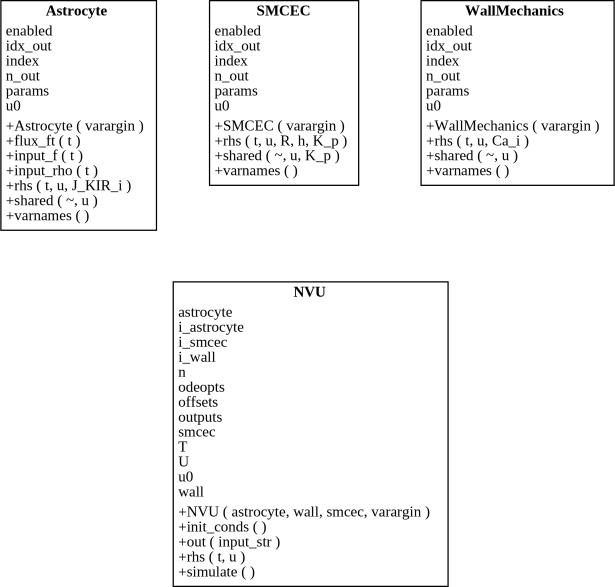
\includegraphics[width=0.7\linewidth]{figures/OO-Code-Structure}
	\caption[OO NVU Classes]{UML class diagram for the OO NVU code.}
	\label{fig:OO-Code-Structure}
\end{figure}

The code in the file \texttt{nvu\_script.m} provides a number of use-cases for running the NVU model. The code Listing~\ref{lst:NVU-Model-Init} shows an example of setting the options for the ODE solver \texttt{ode15s} specifying the \texttt{odeopts} parameter, however the code works well with default tolerances. The \texttt{simulate()} method of the \texttt{NVU} class start the simulation.

\begin{lstlisting}[language=Matlab,caption={Initialisation of the NVU model components.},label={lst:NVU-Model-Init},frameround=tttt,belowcaptionskip=10pt]
odeopts = odeset('RelTol', 1e-03, 'AbsTol', 1e-03, 'MaxStep', 1, 'Vectorized', 1);

nv = NVU(Astrocyte(), ...
WallMechanics(), ...
SMCEC('J_PLC', 0.18), ...
'odeopts', odeopts);

nv.simulate()
\end{lstlisting}



%\documentclass[12pt]{article}
%\usepackage{amsmath,xcolor,todonotes,graphicx,marvosym,dsfont,import,fullpage,textcomp,colortbl,array,pgfplots,lscape}
%\begin{document}
	\section{Results}
	\subsection {NVU1.1}
	\subsubsection*{Potassium input signal (figure \ref{fig:1IS})}
	At the top the neuronal \gls{K} input signal is shown. This input signal is pumped into the SC by the \gls{NE}. As a result of that, there is more \gls{K} taken up by the \gls{AC} in the beginning of the input pulse, and released at the end of the input pulse. In the second graph the membrane potential of the AC is shown over time. When the \gls{K} concentration in the SC is increased the membrane voltage depolarises and when the \gls{K} concentration in the SC decreases the membrane potential repolarises again.
	In the third graph the fluxes into the PVS are shown. In blue the flux by the astrocytic BK channel, and in green the flux by the KIR channel in the SMC is shown. The drop in the middle of the KIR flux is caused because the SMC becomes in a oscillatory state and therefore the efflux by the KIR channel follows the \gls{Ca} waves inside the SMC.
	The bottom figure shows the \gls{K} concentration in the PVS.
	
	\subsubsection*{Solutions of astrocyte and BK-channel equations (figure \ref{fig:7ACe})}
	 The top 4 graphs display the concentrations of \gls{K}, \gls{Ca} \gls{IP3} and EET in the astrocyte. These concentrations, together with the membrane voltage showed in the right bottom graph, all contribute to the opening of the BK-channel in their own way. The open state of the BK channel determines the potassium flux from the astrocyte to the perivascular spcace, where it induces vascular contraction.
	
	\subsubsection*{SMC and EC fluxes (figure \ref{fig:2SMCF} and \ref{fig:3ECF})}
	In these figures the coupling and the fluxes in the SMC and EC are shown. When one of the fluxes is negative, it means that the direction of the flux is in the opposite than it is defined in the equations. These figures show that when the neuronal signal is given, the VOCC closes and that the SMC goes into an oscillatory state. 
	
	\subsubsection*{Conservation equations (figure \ref{fig:4DFDT})}
	The graphs in this figure shows the solutions of the differential equations of the \gls{SMC} and \gls{EC}. The graphs on the left side are the SMC results, and at the right side the EC results. From top to bottom the following parameters are shown over time: the intracellular \gls{Ca} concentration, the \gls{IP3} concentration, the sarcoplasmic (\gls{SMC}) or endoplasmic (\gls{EC}) \gls{Ca} concentration, the membrane voltage and at the bottom for the SMC the open probability of the \gls{K} channels.
	
	\subsubsection*{Hai and Murphy and radius model (figure \ref{fig:5MCm})}
	In this figure the fraction of the four states (M, Mp, AMp, AM) of myosin in the SMC are shown at the top. At the bottom left the fraction of attached cross bridged myosin (the sum of AM and AMp) is shown. And at the bottom right the radius is plotted over time. The increase in vessel diameter is in the expected order of magnitude.
	
	\subsubsection*{Overview from the synaptic cleft to radius change (figure \ref{fig:6NtR})}
	This figure descripes the main pathway from the synaptic cleft to the radius change (leaving out the astrocyte equations which can be found in figure \ref{fig:7ACe}) It starts with a \gls{K} concentration in the synaptic cleft, followed by the flux trough the BK-channel determined in the astrocyte, leading to an increased \gls{K} concentration in the perivascular space. This causes an increased  \gls{K} influx trough the KIR channel, changing the membrane voltage of the SMC. The \gls{Ca} flux through the VOCC increases, decreasing the \gls{Ca} concentration in the SMC and thereby inducing vasodilation. 
		
	
	\begin{landscape}
			
		\begin{figure}[h!]
			\centering
			\tiny 
%			\newlength\figureheight 
%			\newlength\figurewidth 
			\setlength\figureheight{3 cm} 
			\setlength\figurewidth{18 cm}
			%% % This file was created by matlab2tikz v0.3.3.
% Copyright (c) 2008--2013, Nico Schlömer <nico.schloemer@gmail.com>
% All rights reserved.
% 
% The latest updates can be retrieved from
%   http://www.mathworks.com/matlabcentral/fileexchange/22022-matlab2tikz
% where you can also make suggestions and rate matlab2tikz.
% 
% 
% 
\begin{tikzpicture}

\begin{axis}[%
width=\figurewidth,
height=\figureheight,
scale only axis,
xmin=0,
xmax=500,
xlabel={Time [s]},
separate axis lines,
every outer y axis line/.append style={blue},
every y tick label/.append style={font=\color{blue}},
ymin=-5000,
ymax=5000,
ytick={-5000,     0,  5000},
ylabel={$\text{J}_{\text{BK}}\text{ [}\mu\text{M/s]}$},
name=plot3,
title={$\text{The contribution of the BK- and KIR-channel to K}_\text{p}$}
]
\addplot [
color=blue,
solid,
forget plot
]
table[row sep=crcr]{
0 113.285245901639\\
0.0011996 110.367673587195\\
0.0023992 108.143520112822\\
0.0035988 105.901838277496\\
0.0085566 97.0384703683054\\
0.013514 88.9000032796563\\
0.018472 81.4650224656456\\
0.02343 74.6847482085171\\
0.033542 62.7180899908173\\
0.043655 52.9080921538083\\
0.053767 44.8848077396081\\
0.063879 38.3366674318696\\
0.073991 33.011953367111\\
0.084819 28.4187053190792\\
0.095647 24.7548778488277\\
0.10647 21.8376481776\\
0.1173 19.5156741867786\\
0.12813 17.6692407325431\\
0.14659 15.3720796786622\\
0.16505 13.8232015214112\\
0.18351 12.7727138594708\\
0.20197 12.0608196721311\\
0.22042 11.5807937574794\\
0.26398 11.0246701090075\\
0.30753 10.7948137949121\\
0.35108 10.6624926244018\\
0.37397 10.6097061282022\\
0.38969 10.5893729308028\\
0.4054 10.5762517413751\\
0.42111 10.5659171364888\\
0.43393 10.55787731288\\
0.44676 10.5503294109935\\
0.45959 10.5434372900244\\
0.47242 10.5372097215621\\
0.48525 10.5309734513274\\
0.50035 10.5240818734534\\
0.51544 10.5173543967749\\
0.53054 10.5107910132245\\
0.54564 10.5045638529735\\
0.56073 10.4980007865758\\
0.57728 10.4911102007374\\
0.59382 10.4840559761413\\
0.61036 10.477001982729\\
0.6269 10.4701197830468\\
0.64344 10.4632299927902\\
0.65998 10.4561765717937\\
0.69992 10.4391211023906\\
0.73986 10.4222375147464\\
0.77979 10.4050201527018\\
0.81973 10.3881379536332\\
0.85967 10.3709225551715\\
0.99616 10.313068265592\\
1.1327 10.2558768121877\\
1.2692 10.1998427466911\\
1.4056 10.1449607705034\\
1.6062 10.0669887806076\\
1.8067 9.99181106488912\\
2.0072 9.91942483745762\\
2.2078 9.84949969703421\\
2.4083 9.78187177597642\\
2.8551 9.63745926738607\\
3.302 9.50090877830721\\
3.7488 9.36993434087076\\
4.1956 9.24338927548097\\
4.6425 9.12044010740716\\
5.3586 8.92969415154889\\
6.0748 8.74437185847373\\
6.791 8.56361641861912\\
7.5072 8.38648940698778\\
8.2234 8.21277710468581\\
9.2234 7.97521202396935\\
10.223 7.74255869543862\\
11.223 7.51432594387504\\
12.223 7.28904024362291\\
12.523 7.22158551360555\\
12.823 7.15363960836963\\
13.123 7.08487507776941\\
13.423 7.01267232063918\\
13.513 6.98975081043911\\
13.603 6.96568322472903\\
13.693 6.93965093814467\\
13.783 6.91001669995743\\
13.873 6.87366973378303\\
13.929 6.84812862241724\\
13.948 6.84059726906578\\
13.967 6.83683159239006\\
13.986 6.83945119355578\\
14.004 6.84894724778153\\
14.023 6.86581093028586\\
14.079 6.95864304659615\\
14.134 7.10239366056518\\
14.189 7.22338648940699\\
14.244 7.11516421624808\\
14.299 6.54998526474344\\
14.354 5.79865090539965\\
14.409 5.52932316054881\\
14.465 6.08435115753626\\
14.52 7.32325878385016\\
14.575 8.95510658502243\\
14.631 10.7907921019025\\
14.686 12.7111234814499\\
14.742 14.5787353875372\\
14.811 16.6213693965094\\
14.88 18.1440125740856\\
14.95 19.0674219850028\\
15.019 19.4308916467468\\
15.089 19.3342938537608\\
15.202 18.4861979763581\\
15.315 17.1403778774682\\
15.428 15.6142964733619\\
15.541 14.1058973771243\\
15.654 12.7194734601657\\
15.804 11.1493500114608\\
15.954 9.95955990700416\\
16.104 9.18317561151315\\
16.255 8.82494515210059\\
16.405 8.82314417629916\\
16.675 9.14437276924588\\
16.946 9.11981400831723\\
17.216 8.45148826091228\\
17.487 7.69606077474704\\
17.757 7.10190248534661\\
18.061 6.57929205278496\\
18.364 6.16916074527653\\
18.667 5.86233995874128\\
18.971 5.63410720717771\\
19.274 5.45581060283572\\
19.375 5.40636563083271\\
19.476 5.36690788827401\\
19.576 5.33743737515963\\
19.677 5.31533449032385\\
19.778 5.29699728216379\\
19.938 5.26900029470513\\
20.097 5.24149448246504\\
20.257 5.2126788696421\\
20.416 5.182880906382\\
20.576 5.15341039326762\\
20.994 5.0780968597531\\
21.411 5.00016372507286\\
21.828 4.91977471429975\\
22.056 4.87491404433675\\
22.119 4.86361701430957\\
22.183 4.8546121353024\\
22.247 4.84953665804381\\
22.31 4.84740823209666\\
22.432 4.84822685746095\\
22.554 4.85199253413668\\
22.676 4.85919643734241\\
22.798 4.87032974229674\\
22.92 4.88424637348964\\
23.367 4.94744425161269\\
23.684 5.00278332623858\\
24 5.05959592652019\\
24.242 5.09921739415174\\
24.484 5.13048888306755\\
24.726 5.14948099151904\\
24.968 5.15308294312191\\
25.298 5.13048888306755\\
25.628 5.07564098366024\\
25.958 4.99165002128426\\
26.288 4.88539244899964\\
26.618 4.7648907953764\\
27.087 4.58364713972298\\
27.556 4.4056779855267\\
28.025 4.24064311208619\\
28.494 4.09279937129572\\
28.964 3.96198303808245\\
29.615 3.80578931857625\\
30.266 3.67431808507155\\
30.917 3.56167523494548\\
31.569 3.46180294050231\\
32.372 3.34752283964766\\
33.175 3.2329152886473\\
33.979 3.10913913356691\\
34.782 2.97226497265791\\
35.586 2.82458495694031\\
36.23 2.70228232751564\\
36.875 2.58030714823668\\
37.52 2.46078784505059\\
38.164 2.34487049346737\\
38.969 2.20603163168408\\
39.774 2.0729231474508\\
40.579 1.94439896525754\\
41.384 1.81865810930286\\
42.189 1.6943907790039\\
43.189 1.54114411080913\\
44.189 1.38912538066079\\
45.189 1.23933331150332\\
46.189 1.09296309636858\\
47.189 0.950882478142703\\
48.189 0.813386161956842\\
49.189 0.680294050230852\\
50.189 0.551164085268018\\
51.189 0.425717934444481\\
52.189 0.303742755165526\\
53.189 0.185074822358296\\
54.189 0.0695798814630473\\
55.189 -0.042900880840892\\
56.189 -0.152554111136579\\
57.189 -0.25956973050853\\
58.189 -0.36412456203543\\
59.189 -0.466354497527751\\
60.189 -0.566325027014637\\
61.189 -0.664118013032516\\
62.189 -0.759782573103245\\
63.189 -0.853351452241396\\
64.189 -0.944890140476112\\
65.189 -1.03444775532925\\
66.189 -1.12212253184453\\
67.189 -1.20791447002194\\
68.189 -1.29185631487606\\
69.189 -1.37348963620289\\
70.189 -1.45324011919185\\
71.189 -1.5311732538721\\
72.189 -1.60764923540391\\
73.189 -1.68243884868529\\
74.189 -1.75562395625266\\
75.189 -1.82717181309146\\
76.189 -1.8965912439831\\
77.189 -1.96437342414617\\
78.189 -2.03051835358067\\
79.189 -2.09518975735944\\
80.189 -2.1583876354825\\
81.189 -2.21994826287698\\
82.189 -2.28052653983431\\
83.189 -2.33979501620878\\
84.189 -2.39791741707325\\
85.189 -2.454566292282\\
86.189 -2.50957791676217\\
87.189 -2.56344346573234\\
88.189 -2.61616293919251\\
89.189 -2.66757261206981\\
90.189 -2.71783620943711\\
91.189 -2.76711745636727\\
92.189 -2.81525262778742\\
93.189 -2.86240544877042\\
94.189 -2.90857591931628\\
95.189 -2.95360031435214\\
96.189 -2.99780608402371\\
97.189 -3.04086577818527\\
98.189 -3.08310684698255\\
99.189 -3.12436556534268\\
100.19 -3.16480565833852\\
101.19 -3.20426340089721\\
102.19 -3.24290251809162\\
103.19 -3.28072300992174\\
104.19 -3.31772487638757\\
105.19 -3.35374439241625\\
106.19 -3.38927273322637\\
107.19 -3.42381872359933\\
108.19 -3.45770981368087\\
109.19 -3.49078227839811\\
110.19 -3.52319984282393\\
111.19 -3.55479878188546\\
112.19 -3.58590654572841\\
113.19 -3.61619568420708\\
114.19 -3.64582992239432\\
115.19 -3.67480926029012\\
116.19 -3.70329742296735\\
117.19 -3.73113068535315\\
118.19 -3.75830904744753\\
119.19 -3.78483250925047\\
120.19 -3.81102852090769\\
121.19 -3.83640590720063\\
122.19 -3.86129211827499\\
123.19 -3.88585087920364\\
124.19 -3.909591014768\\
125.19 -3.93300370018665\\
126.19 -3.95592521038672\\
127.19 -3.97819182029536\\
128.19 -4.00013098005829\\
129.19 -4.02157896460264\\
130.19 -4.04253577392842\\
131.19 -4.06316513310848\\
132.19 -4.08313959199712\\
133.19 -4.10278660074004\\
134.19 -4.12210615933724\\
135.19 -4.14093454271587\\
136.19 -4.15927175087593\\
137.19 -4.17744523396313\\
138.19 -4.1949638167589\\
139.19 -4.21231867448181\\
140.19 -4.22918235698615\\
141.19 -4.24571858934477\\
142.19 -4.26192737155768\\
143.19 -4.27780870362487\\
144.19 -4.29336258554635\\
145.19 -4.30842529224925\\
146.19 -4.3233242738793\\
147.19 -4.33789580536363\\
148.19 -4.35213988670225\\
149.19 -4.36605651789515\\
150.19 -4.37964569894234\\
151.19 -4.39307115491666\\
152.19 -4.40616916074528\\
153.19 -4.41893971642817\\
154.19 -4.43154654703821\\
155.19 -4.44366220242968\\
156.19 -4.45577785782115\\
157.19 -4.46740233799404\\
158.19 -4.47902681816693\\
159.19 -4.49016012312125\\
160.19 -4.50129342807558\\
161.19 -4.51193555781132\\
162.19 -4.52257768754707\\
163.19 -4.5328923671371\\
164.19 -4.54304332165428\\
165.19 -4.55286682602574\\
166.19 -4.5626903303972\\
167.19 -4.57202265955008\\
168.19 -4.58135498870297\\
169.19 -4.590523592783\\
170.19 -4.59936474671731\\
171.19 -4.60804217557877\\
172.19 -4.61655587936737\\
173.19 -4.62490585808311\\
174.19 -4.63309211172599\\
175.19 -4.64111464029601\\
176.19 -4.64897344379318\\
177.19 -4.65666852221749\\
178.19 -4.66419987556894\\
179.19 -4.67156750384754\\
180.19 -4.67877140705328\\
181.19 -4.68581158518615\\
182.19 -4.69268803824618\\
183.19 -4.69940076623334\\
184.19 -4.70594976914765\\
185.19 -4.71249877206195\\
186.19 -4.7188840499034\\
187.19 -4.72494187759914\\
188.19 -4.73116343036773\\
189.19 -4.7370575329906\\
190.19 -4.74278791054062\\
191.19 -4.74851828809064\\
192.19 -4.7540849405678\\
193.19 -4.75965159304496\\
194.19 -4.7648907953764\\
195.19 -4.77029372278071\\
196.19 -4.77602410033072\\
196.81 -4.78093585251645\\
197.25 -4.78601132977504\\
197.57 -4.7915779822522\\
197.82 -4.79779953502079\\
198.03 -4.80483971315367\\
198.24 -4.81499066767085\\
198.38 -4.8236680965323\\
198.52 -4.83512885163234\\
198.63 -4.84593470644094\\
198.74 -4.85952388748813\\
198.83 -4.87245816824388\\
198.92 -4.8878483250925\\
199.01 -4.9060218081797\\
199.17 -4.94220504928125\\
199.32 -4.98870296997282\\
199.47 -5.04813517142015\\
199.62 -5.12312125478896\\
199.84 -5.26179639149939\\
200.07 -6.80932452756163\\
200.29 -3.698143348493\\
200.51 5.68713758994266\\
200.69 18.395829285668\\
200.87 35.2024268633114\\
201.05 58.7831427974209\\
201.23 93.9399279134962\\
201.42 144.71660177443\\
201.6 215.844259038538\\
201.79 312.196357076166\\
201.97 441.597731032853\\
202.15 610.281429423023\\
202.34 819.059220389805\\
202.63 1214.78414588761\\
202.92 1652.57825611653\\
203.21 2066.9092688297\\
203.5 2388.53116267768\\
203.79 2566.83765841883\\
204.09 2582.37145855194\\
204.39 2443.30879942787\\
204.69 2189.33333333333\\
204.94 1928.51769356718\\
205.19 1636.79370023213\\
205.44 1333.06986343477\\
205.68 1041.05032822757\\
205.85 855.362757656923\\
206.02 685.020266441968\\
206.19 531.395011600928\\
206.36 395.051898605903\\
206.6 230.467000823354\\
206.84 98.2050949353402\\
207.08 -5.35614052762626\\
207.32 -84.5567946654403\\
207.65 -162.085389647653\\
207.99 -211.773470294122\\
208.32 -241.800228963938\\
208.65 -258.16367379618\\
208.99 -265.272301274359\\
209.66 -263.286334056399\\
210.18 -254.735280693747\\
210.7 -244.104815944798\\
211.22 -232.911464568725\\
211.74 -221.82958107723\\
212.26 -210.949965808069\\
212.9 -197.54141560902\\
213.54 -184.190286284005\\
214.18 -171.273944313893\\
214.82 -159.104503118858\\
215.46 -147.949302193107\\
216.16 -137.009769018256\\
216.87 -127.533714025319\\
217.57 -119.35378218273\\
218.27 -112.146844383686\\
218.98 -105.597721609114\\
219.98 -97.3470986116056\\
220.98 -90.1488074047704\\
221.98 -84.1139195443218\\
222.98 -79.4788180847277\\
223.98 -76.0085439658241\\
224.98 -73.1947312210751\\
225.98 -70.8209327162691\\
226.98 -68.6322534709861\\
227.98 -66.752580989676\\
228.98 -65.1776432894268\\
229.98 -63.9729441082236\\
230.98 -63.0672837308651\\
231.98 -62.3367746529014\\
232.98 -61.6988252046992\\
233.98 -61.0964756140975\\
234.98 -60.5710217159131\\
235.98 -60.2321110715557\\
236.98 -59.8049127803489\\
237.98 -59.6682093271627\\
238.98 -59.4802420790317\\
239.98 -59.3179067283731\\
240.98 -59.1584193663225\\
241.98 -59.0530437878248\\
242.98 -58.939124243503\\
243.98 -58.8593805624778\\
244.98 -58.7796368814525\\
245.98 -58.7255250978996\\
246.98 -58.6728373086508\\
247.98 -58.6372374510502\\
248.98 -58.6016375934496\\
249.98 -58.5774296902812\\
250.98 -58.5546457814169\\
251.98 -58.5375578497686\\
252.98 -58.5218939124244\\
253.98 -58.5105019579922\\
254.98 -58.49911000356\\
255.98 -58.4919900320399\\
256.98 -58.4848700605198\\
257.98 -58.4791740833037\\
258.98 -58.4749021003916\\
259.98 -58.4706301174795\\
260.98 -58.4677821288715\\
261.98 -58.4649341402634\\
262.98 -58.4620861516554\\
263.98 -58.4606621573514\\
264.98 -58.4592381630474\\
265.98 -58.4578141687433\\
266.98 -58.4563901744393\\
267.98 -58.4549661801353\\
268.98 -58.4535421858313\\
269.98 -58.4535421858313\\
270.98 -58.4521181915272\\
271.98 -58.4521181915272\\
272.98 -58.4506941972232\\
273.98 -58.4506941972232\\
274.98 -58.4492702029192\\
275.98 -58.4492702029192\\
276.98 -58.4492702029192\\
277.98 -58.4478462086152\\
278.98 -58.4478462086152\\
279.98 -58.4478462086152\\
280.98 -58.4478462086152\\
281.98 -58.4464222143111\\
282.98 -58.4464222143111\\
283.98 -58.4464222143111\\
284.98 -58.4464222143111\\
285.98 -58.4464222143111\\
286.98 -58.4449982200071\\
287.98 -58.4449982200071\\
288.98 -58.4449982200071\\
289.98 -58.4449982200071\\
290.98 -58.4449982200071\\
291.98 -58.4435742257031\\
292.98 -58.4435742257031\\
293.98 -58.4435742257031\\
294.98 -58.4435742257031\\
295.98 -58.4435742257031\\
296.98 -58.4435742257031\\
297.98 -58.4435742257031\\
298.98 -58.4421502313991\\
299.98 -58.4421502313991\\
300.98 -58.4421502313991\\
301.98 -58.4421502313991\\
302.98 -58.4421502313991\\
303.98 -58.4421502313991\\
304.98 -58.4421502313991\\
305.98 -58.4407262370951\\
306.98 -58.4407262370951\\
307.98 -58.4407262370951\\
308.98 -58.4407262370951\\
309.98 -58.4407262370951\\
310.98 -58.4407262370951\\
311.98 -58.4407262370951\\
312.98 -58.4407262370951\\
313.98 -58.4407262370951\\
314.98 -58.439302242791\\
315.98 -58.439302242791\\
316.98 -58.439302242791\\
317.98 -58.439302242791\\
318.98 -58.439302242791\\
319.98 -58.439302242791\\
320.98 -58.439302242791\\
321.98 -58.439302242791\\
322.98 -58.439302242791\\
323.98 -58.439302242791\\
324.98 -58.439302242791\\
325.98 -58.437878248487\\
326.98 -58.437878248487\\
327.98 -58.437878248487\\
328.98 -58.437878248487\\
329.98 -58.437878248487\\
330.98 -58.437878248487\\
331.98 -58.437878248487\\
332.98 -58.437878248487\\
333.98 -58.437878248487\\
334.98 -58.437878248487\\
335.98 -58.437878248487\\
336.98 -58.437878248487\\
337.98 -58.437878248487\\
338.98 -58.437878248487\\
339.98 -58.437878248487\\
340.98 -58.436454254183\\
341.98 -58.436454254183\\
342.98 -58.436454254183\\
343.98 -58.436454254183\\
344.98 -58.436454254183\\
345.98 -58.436454254183\\
346.98 -58.436454254183\\
347.98 -58.436454254183\\
348.98 -58.436454254183\\
349.98 -58.436454254183\\
350.98 -58.436454254183\\
351.98 -58.436454254183\\
352.98 -58.436454254183\\
353.98 -58.436454254183\\
354.98 -58.436454254183\\
355.98 -58.436454254183\\
356.98 -58.436454254183\\
357.98 -58.436454254183\\
358.98 -58.436454254183\\
359.98 -58.436454254183\\
360.98 -58.436454254183\\
361.98 -58.436454254183\\
362.98 -58.436454254183\\
363.98 -58.436454254183\\
364.98 -58.435030259879\\
365.98 -58.435030259879\\
366.98 -58.435030259879\\
367.98 -58.435030259879\\
368.98 -58.435030259879\\
369.98 -58.435030259879\\
370.98 -58.435030259879\\
371.98 -58.435030259879\\
372.98 -58.435030259879\\
373.98 -58.435030259879\\
374.98 -58.435030259879\\
375.98 -58.435030259879\\
376.98 -58.435030259879\\
377.98 -58.435030259879\\
378.98 -58.435030259879\\
379.98 -58.435030259879\\
380.98 -58.435030259879\\
381.98 -58.435030259879\\
382.98 -58.435030259879\\
383.98 -58.435030259879\\
384.98 -58.435030259879\\
385.98 -58.435030259879\\
386.98 -58.435030259879\\
387.98 -58.435030259879\\
388.98 -58.435030259879\\
389.98 -58.435030259879\\
390.98 -58.435030259879\\
391.98 -58.435030259879\\
392.98 -58.435030259879\\
393.98 -58.435030259879\\
394.98 -58.435030259879\\
395.98 -58.4336062655749\\
396.98 -58.4264862940548\\
397.98 -58.4649341402634\\
398.44 -58.4706301174795\\
398.8 -58.4734781060876\\
399.07 -58.4720541117836\\
399.35 -58.4008543965824\\
399.55 -58.4093983624066\\
399.76 -58.3396226415094\\
399.96 -58.2840868636525\\
400.26 -209.25791326407\\
400.34 -238.461209416395\\
400.43 -244.664155681105\\
400.52 -241.287743593404\\
400.61 -236.81353220184\\
400.92 -224.96633527204\\
401.24 -218.547042933502\\
401.56 -207.533298737243\\
401.87 -192.495732924466\\
402.11 -180.9387056537\\
402.35 -170.363475048362\\
402.59 -160.569461462162\\
402.83 -151.369301890105\\
403.14 -140.318388086881\\
403.45 -130.55567841715\\
403.77 -122.229458695363\\
404.08 -114.926437806509\\
404.39 -108.504923903312\\
404.93 -98.5875706214689\\
405.47 -88.969253117056\\
406.02 -80.1084853194374\\
406.56 -74.5060137457045\\
407.1 -72.7115476686898\\
408.1 -63.4064766191548\\
408.77 -57.3057239587434\\
409.43 -52.9736416404986\\
410.1 -68.3297110713372\\
410.61 -80.5382823170242\\
411.12 -82.0098134159726\\
411.63 -82.4234375759146\\
412.15 -85.5104227547243\\
412.66 -85.6043973914882\\
413.31 -84.3292454520285\\
413.95 -84.0940953995631\\
414.6 -84.3123501296837\\
415.25 -84.2178269525768\\
415.9 -84.1486704862641\\
416.77 -84.279440335668\\
417.65 -84.3856641358478\\
418.52 -84.2964680524485\\
419.4 -83.9905942291677\\
420.28 -83.4710473888762\\
421.2 -82.7558052189817\\
422.12 -82.009242778059\\
423.04 -81.3315479203749\\
423.96 -80.7469340431439\\
424.89 -80.2390711497951\\
425.81 -79.7671342489018\\
426.73 -79.2853993500661\\
427.68 -78.7628394598037\\
428.64 -78.2059865767428\\
429.59 -77.6213726995117\\
430.55 -77.0171628263958\\
431.5 -76.4129529532799\\
432.5 -75.7891470842791\\
433.5 -75.1784052125349\\
434.5 -74.5774613387331\\
435.5 -73.9781504645884\\
436.5 -73.3739405914725\\
437.5 -72.7599327204141\\
438.5 -72.1393928507275\\
439.5 -71.5139539820697\\
440.5 -70.8885151134118\\
441.5 -70.2614432450969\\
442.5 -69.6376373760962\\
443.5 -69.0138315070954\\
444.5 -68.3900256380946\\
445.5 -67.7645867694368\\
446.5 -67.1375149011219\\
447.5 -66.5071770334928\\
448.5 -65.8768391658638\\
449.5 -65.2448682985777\\
450.5 -64.6128974312915\\
451.5 -63.9792935643484\\
452.5 -63.3473226970622\\
453.5 -62.713718830119\\
454.5 -62.0817479628329\\
455.5 -61.4497770955468\\
456.5 -60.8178062282607\\
457.5 -60.1874683606316\\
458.5 -59.5571304930026\\
459.5 -58.9267926253736\\
460.5 -58.2980877574016\\
461.5 -57.6710158890867\\
462.5 -57.0439440207718\\
463.5 -56.420138151771\\
464.5 -55.7963322827702\\
465.5 -55.1757924130836\\
466.5 -54.556885543054\\
467.5 -53.9396116726815\\
468.5 -53.3239708019661\\
469.5 -52.7115959305649\\
470.5 -52.1008540588207\\
471.5 -51.4933781863906\\
472.5 -50.8875353136176\\
473.5 -50.2849584401587\\
474.5 -49.685647566014\\
475.5 -49.0896026911834\\
476.5 -48.496823815667\\
477.5 -47.9056779398076\\
478.5 -47.3194310629195\\
479.5 -46.7364501853455\\
480.5 -46.1567353070856\\
481.5 -45.5802864281399\\
482.5 -45.0071035485083\\
483.5 -44.4388196678479\\
484.5 -43.8738017865016\\
485.5 -43.3136829041266\\
486.5 -42.7568300210657\\
487.5 -42.204876136976\\
488.5 -41.6561882522005\\
489.5 -41.1107663667391\\
490.5 -40.5718764799059\\
491.5 -40.036252592387\\
492.5 -39.5055277038392\\
493.5 -38.9797018142626\\
494.5 -38.4571419240002\\
495.5 -37.939481032709\\
496.5 -37.4283521400461\\
497.5 -36.9204892466973\\
498.5 -36.4175253523197\\
499.5 -35.9194604569133\\
500 -35.6728775086957\\
};
\end{axis}

\begin{axis}[%
width=\figurewidth,
height=\figureheight,
scale only axis,
xmin=0,
xmax=500,
every outer y axis line/.append style={green!50!black},
every y tick label/.append style={font=\color{green!50!black}},
ymin=0,
ymax=100,
ytick={  0,  50, 100},
ylabel={$\text{J}_{\text{KIR}}\text{ [}\mu\text{M/s]}$},
axis x line*=bottom,
axis y line*=right
]
\addplot [
color=green!50!black,
solid,
forget plot
]
table[row sep=crcr]{
0 14.771\\
0.0011996 14.705\\
0.0023992 14.638\\
0.0035988 14.569\\
0.0085566 14.275\\
0.013514 13.968\\
0.018472 13.652\\
0.02343 13.332\\
0.033542 12.679\\
0.043655 12.043\\
0.053767 11.433\\
0.063879 10.855\\
0.073991 10.311\\
0.084819 9.7636\\
0.095647 9.2522\\
0.10647 8.7738\\
0.1173 8.3255\\
0.12813 7.9045\\
0.14659 7.2413\\
0.16505 6.6359\\
0.18351 6.0767\\
0.20197 5.5539\\
0.22042 5.0585\\
0.26398 3.951\\
0.30753 2.8752\\
0.35108 1.8495\\
0.37397 1.3876\\
0.38969 1.1294\\
0.4054 0.93013\\
0.42111 0.7875\\
0.43393 0.70697\\
0.44676 0.65189\\
0.45959 0.61626\\
0.47242 0.59501\\
0.48525 0.58409\\
0.50035 0.58027\\
0.51544 0.58265\\
0.53054 0.58861\\
0.54564 0.5964\\
0.56073 0.60498\\
0.57728 0.61456\\
0.59382 0.62399\\
0.61036 0.63314\\
0.6269 0.64198\\
0.64344 0.65053\\
0.65998 0.65883\\
0.69992 0.67813\\
0.73986 0.69679\\
0.77979 0.71507\\
0.81973 0.73296\\
0.85967 0.75039\\
0.99616 0.80669\\
1.1327 0.85778\\
1.2692 0.90388\\
1.4056 0.94522\\
1.6062 0.99774\\
1.8067 1.0415\\
2.0072 1.0777\\
2.2078 1.1074\\
2.4083 1.132\\
2.8551 1.1736\\
3.302 1.2044\\
3.7488 1.2292\\
4.1956 1.2509\\
4.6425 1.2714\\
5.3586 1.3044\\
6.0748 1.3384\\
6.791 1.373\\
7.5072 1.409\\
8.2234 1.4477\\
9.2234 1.5062\\
10.223 1.568\\
11.223 1.6326\\
12.223 1.7049\\
12.523 1.729\\
12.823 1.7531\\
13.123 1.7771\\
13.423 1.8015\\
13.513 1.809\\
13.603 1.8167\\
13.693 1.8243\\
13.783 1.832\\
13.873 1.8398\\
13.929 1.8446\\
13.948 1.8462\\
13.967 1.8479\\
13.986 1.8495\\
14.004 1.8512\\
14.023 1.8529\\
14.079 1.8577\\
14.134 1.8626\\
14.189 1.8675\\
14.244 1.8724\\
14.299 1.8773\\
14.354 1.8823\\
14.409 1.8872\\
14.465 1.8922\\
14.52 1.8972\\
14.575 1.9023\\
14.631 1.9076\\
14.686 1.9129\\
14.742 1.9183\\
14.811 1.9252\\
14.88 1.9322\\
14.95 1.9394\\
15.019 1.9466\\
15.089 1.9538\\
15.202 1.9657\\
15.315 1.9776\\
15.428 1.9895\\
15.541 2.0013\\
15.654 2.0131\\
15.804 2.0289\\
15.954 2.0446\\
16.104 2.0604\\
16.255 2.0763\\
16.405 2.0924\\
16.675 2.1217\\
16.946 2.1517\\
17.216 2.1821\\
17.487 2.2129\\
17.757 2.244\\
18.061 2.2793\\
18.364 2.315\\
18.667 2.3511\\
18.971 2.3877\\
19.274 2.4246\\
19.375 2.4369\\
19.476 2.4493\\
19.576 2.4617\\
19.677 2.4742\\
19.778 2.4867\\
19.938 2.5065\\
20.097 2.5265\\
20.257 2.5465\\
20.416 2.5665\\
20.576 2.5866\\
20.994 2.6394\\
21.411 2.6924\\
21.828 2.7454\\
22.056 2.7743\\
22.119 2.7824\\
22.183 2.7905\\
22.247 2.7986\\
22.31 2.8066\\
22.432 2.8221\\
22.554 2.8375\\
22.676 2.8529\\
22.798 2.8683\\
22.92 2.8837\\
23.367 2.9399\\
23.684 2.9795\\
24 3.0189\\
24.242 3.0489\\
24.484 3.0787\\
24.726 3.1083\\
24.968 3.1377\\
25.298 3.1776\\
25.628 3.217\\
25.958 3.256\\
26.288 3.2945\\
26.618 3.3326\\
27.087 3.3859\\
27.556 3.4382\\
28.025 3.4894\\
28.494 3.5396\\
28.964 3.5888\\
29.615 3.6553\\
30.266 3.7199\\
30.917 3.7826\\
31.569 3.8435\\
32.372 3.916\\
33.175 3.986\\
33.979 4.0534\\
34.782 4.1185\\
35.586 4.1814\\
36.23 4.2304\\
36.875 4.2781\\
37.52 4.3244\\
38.164 4.3694\\
38.969 4.4234\\
39.774 4.4746\\
40.579 4.5224\\
41.384 4.566\\
42.189 4.6044\\
43.189 4.6435\\
44.189 4.6713\\
45.189 4.6869\\
46.189 4.6904\\
47.189 4.6832\\
48.189 4.6681\\
49.189 4.6487\\
50.189 4.6291\\
51.189 4.6112\\
52.189 4.5975\\
53.189 4.5888\\
54.189 4.5853\\
55.189 4.5866\\
56.189 4.5918\\
57.189 4.6002\\
58.189 4.6109\\
59.189 4.6231\\
60.189 4.6364\\
61.189 4.6504\\
62.189 4.6645\\
63.189 4.6787\\
64.189 4.6925\\
65.189 4.7056\\
66.189 4.7179\\
67.189 4.7291\\
68.189 4.7394\\
69.189 4.7481\\
70.189 4.7558\\
71.189 4.7624\\
72.189 4.7683\\
73.189 4.7732\\
74.189 4.7774\\
75.189 4.7811\\
76.189 4.7842\\
77.189 4.7873\\
78.189 4.7904\\
79.189 4.7935\\
80.189 4.7967\\
81.189 4.8\\
82.189 4.8034\\
83.189 4.807\\
84.189 4.8108\\
85.189 4.8148\\
86.189 4.8189\\
87.189 4.8231\\
88.189 4.8273\\
89.189 4.8315\\
90.189 4.8356\\
91.189 4.8398\\
92.189 4.8439\\
93.189 4.848\\
94.189 4.8519\\
95.189 4.8558\\
96.189 4.8594\\
97.189 4.863\\
98.189 4.8663\\
99.189 4.8696\\
100.19 4.8727\\
101.19 4.8757\\
102.19 4.8785\\
103.19 4.8813\\
104.19 4.884\\
105.19 4.8866\\
106.19 4.8891\\
107.19 4.8916\\
108.19 4.8941\\
109.19 4.8966\\
110.19 4.899\\
111.19 4.9013\\
112.19 4.9037\\
113.19 4.9059\\
114.19 4.9082\\
115.19 4.9104\\
116.19 4.9127\\
117.19 4.9148\\
118.19 4.9169\\
119.19 4.919\\
120.19 4.921\\
121.19 4.923\\
122.19 4.925\\
123.19 4.9269\\
124.19 4.9287\\
125.19 4.9305\\
126.19 4.9323\\
127.19 4.934\\
128.19 4.9357\\
129.19 4.9374\\
130.19 4.939\\
131.19 4.9406\\
132.19 4.9422\\
133.19 4.9437\\
134.19 4.9452\\
135.19 4.9466\\
136.19 4.948\\
137.19 4.9494\\
138.19 4.9508\\
139.19 4.9521\\
140.19 4.9534\\
141.19 4.9547\\
142.19 4.956\\
143.19 4.9572\\
144.19 4.9584\\
145.19 4.9596\\
146.19 4.9608\\
147.19 4.9619\\
148.19 4.963\\
149.19 4.9641\\
150.19 4.9652\\
151.19 4.9662\\
152.19 4.9672\\
153.19 4.9683\\
154.19 4.9692\\
155.19 4.9702\\
156.19 4.9711\\
157.19 4.9721\\
158.19 4.973\\
159.19 4.9738\\
160.19 4.9747\\
161.19 4.9755\\
162.19 4.9764\\
163.19 4.9772\\
164.19 4.978\\
165.19 4.9787\\
166.19 4.9795\\
167.19 4.9802\\
168.19 4.981\\
169.19 4.9817\\
170.19 4.9824\\
171.19 4.9831\\
172.19 4.9838\\
173.19 4.9844\\
174.19 4.9851\\
175.19 4.9857\\
176.19 4.9863\\
177.19 4.9869\\
178.19 4.9875\\
179.19 4.9881\\
180.19 4.9886\\
181.19 4.9892\\
182.19 4.9897\\
183.19 4.9902\\
184.19 4.9908\\
185.19 4.9913\\
186.19 4.9918\\
187.19 4.9923\\
188.19 4.9928\\
189.19 4.9932\\
190.19 4.9937\\
191.19 4.9941\\
192.19 4.9946\\
193.19 4.995\\
194.19 4.9954\\
195.19 4.9958\\
196.19 4.9962\\
196.81 4.9965\\
197.25 4.9966\\
197.57 4.9968\\
197.82 4.9969\\
198.03 4.9969\\
198.24 4.997\\
198.38 4.9971\\
198.52 4.9971\\
198.63 4.9971\\
198.74 4.9972\\
198.83 4.9972\\
198.92 4.9972\\
199.01 4.9972\\
199.17 4.9972\\
199.32 4.9972\\
199.47 4.9972\\
199.62 4.9972\\
199.84 4.9971\\
200.07 4.9967\\
200.29 4.9966\\
200.51 4.9991\\
200.69 5.0049\\
200.87 5.0155\\
201.05 5.0328\\
201.23 5.0604\\
201.42 5.1031\\
201.6 5.1686\\
201.79 5.2648\\
201.97 5.4046\\
202.15 5.6057\\
202.34 5.8911\\
202.63 6.5828\\
202.92 7.7084\\
203.21 9.4871\\
203.5 12.23\\
203.79 16.364\\
204.09 22.713\\
204.39 31.815\\
204.69 43.67\\
204.94 53.635\\
205.19 60.083\\
205.44 61.754\\
205.68 61.271\\
205.85 60.828\\
206.02 60.372\\
206.19 59.916\\
206.36 59.506\\
206.6 59.074\\
206.84 58.817\\
207.08 58.684\\
207.32 58.637\\
207.65 58.67\\
207.99 58.808\\
208.32 59.026\\
208.65 59.267\\
208.99 59.503\\
209.66 59.923\\
210.18 60.194\\
210.7 60.424\\
211.22 60.603\\
211.74 60.729\\
212.26 60.811\\
212.9 60.861\\
213.54 60.859\\
214.18 60.813\\
214.82 60.732\\
215.46 60.627\\
216.16 60.496\\
216.87 60.355\\
217.57 60.211\\
218.27 60.067\\
218.98 59.924\\
219.98 59.726\\
220.98 59.539\\
221.98 59.368\\
222.98 59.224\\
223.98 59.109\\
224.98 59.014\\
225.98 58.932\\
226.98 58.858\\
227.98 58.792\\
228.98 58.733\\
229.98 58.686\\
230.98 58.65\\
231.98 58.621\\
232.98 58.596\\
233.98 58.572\\
234.98 58.552\\
235.98 58.536\\
236.98 58.521\\
237.98 58.512\\
238.98 58.504\\
239.98 58.497\\
240.98 58.49\\
241.98 58.485\\
242.98 58.48\\
243.98 58.476\\
244.98 58.473\\
245.98 58.47\\
246.98 58.467\\
247.98 58.465\\
248.98 58.463\\
249.98 58.462\\
250.98 58.461\\
251.98 58.459\\
252.98 58.458\\
253.98 58.458\\
254.98 58.457\\
255.98 58.456\\
256.98 58.455\\
257.98 58.455\\
258.98 58.454\\
259.98 58.453\\
260.98 58.453\\
261.98 58.452\\
262.98 58.452\\
263.98 58.451\\
264.98 58.451\\
265.98 58.451\\
266.98 58.45\\
267.98 58.45\\
268.98 58.449\\
269.98 58.449\\
270.98 58.449\\
271.98 58.448\\
272.98 58.448\\
273.98 58.447\\
274.98 58.447\\
275.98 58.447\\
276.98 58.447\\
277.98 58.446\\
278.98 58.446\\
279.98 58.446\\
280.98 58.445\\
281.98 58.445\\
282.98 58.445\\
283.98 58.445\\
284.98 58.444\\
285.98 58.444\\
286.98 58.444\\
287.98 58.444\\
288.98 58.443\\
289.98 58.443\\
290.98 58.443\\
291.98 58.443\\
292.98 58.443\\
293.98 58.442\\
294.98 58.442\\
295.98 58.442\\
296.98 58.442\\
297.98 58.442\\
298.98 58.441\\
299.98 58.441\\
300.98 58.441\\
301.98 58.441\\
302.98 58.441\\
303.98 58.44\\
304.98 58.44\\
305.98 58.44\\
306.98 58.44\\
307.98 58.44\\
308.98 58.44\\
309.98 58.44\\
310.98 58.439\\
311.98 58.439\\
312.98 58.439\\
313.98 58.439\\
314.98 58.439\\
315.98 58.439\\
316.98 58.439\\
317.98 58.439\\
318.98 58.438\\
319.98 58.438\\
320.98 58.438\\
321.98 58.438\\
322.98 58.438\\
323.98 58.438\\
324.98 58.438\\
325.98 58.438\\
326.98 58.438\\
327.98 58.438\\
328.98 58.437\\
329.98 58.437\\
330.98 58.437\\
331.98 58.437\\
332.98 58.437\\
333.98 58.437\\
334.98 58.437\\
335.98 58.437\\
336.98 58.437\\
337.98 58.437\\
338.98 58.437\\
339.98 58.437\\
340.98 58.436\\
341.98 58.436\\
342.98 58.436\\
343.98 58.436\\
344.98 58.436\\
345.98 58.436\\
346.98 58.436\\
347.98 58.436\\
348.98 58.436\\
349.98 58.436\\
350.98 58.436\\
351.98 58.436\\
352.98 58.436\\
353.98 58.436\\
354.98 58.436\\
355.98 58.436\\
356.98 58.436\\
357.98 58.435\\
358.98 58.435\\
359.98 58.435\\
360.98 58.435\\
361.98 58.435\\
362.98 58.435\\
363.98 58.435\\
364.98 58.435\\
365.98 58.435\\
366.98 58.435\\
367.98 58.435\\
368.98 58.435\\
369.98 58.435\\
370.98 58.435\\
371.98 58.435\\
372.98 58.435\\
373.98 58.435\\
374.98 58.435\\
375.98 58.435\\
376.98 58.435\\
377.98 58.435\\
378.98 58.435\\
379.98 58.435\\
380.98 58.435\\
381.98 58.435\\
382.98 58.435\\
383.98 58.435\\
384.98 58.435\\
385.98 58.435\\
386.98 58.435\\
387.98 58.435\\
388.98 58.434\\
389.98 58.434\\
390.98 58.434\\
391.98 58.434\\
392.98 58.434\\
393.98 58.434\\
394.98 58.434\\
395.98 58.434\\
396.98 58.434\\
397.98 58.435\\
398.44 58.436\\
398.8 58.436\\
399.07 58.437\\
399.35 58.436\\
399.55 58.436\\
399.76 58.436\\
399.96 58.436\\
400.26 58.244\\
400.34 58.135\\
400.43 58.009\\
400.52 57.872\\
400.61 57.73\\
400.92 57.203\\
401.24 56.641\\
401.56 56.056\\
401.87 55.463\\
402.11 55.015\\
402.35 54.573\\
402.59 54.142\\
402.83 53.722\\
403.14 53.199\\
403.45 52.7\\
403.77 52.226\\
404.08 51.777\\
404.39 51.353\\
404.93 50.67\\
405.47 50.054\\
406.02 49.497\\
406.56 48.999\\
407.1 48.568\\
408.1 47.946\\
408.77 47.655\\
409.43 47.456\\
410.1 47.215\\
410.61 46.901\\
411.12 46.459\\
411.63 45.921\\
412.15 45.313\\
412.66 44.65\\
413.31 43.751\\
413.95 42.79\\
414.6 41.765\\
415.25 40.67\\
415.9 39.504\\
416.77 37.816\\
417.65 36.033\\
418.52 34.251\\
419.4 32.683\\
420.28 31.634\\
421.2 31.21\\
422.12 31.184\\
423.04 31.041\\
423.96 30.473\\
424.89 29.629\\
425.81 28.875\\
426.73 28.398\\
427.68 28.069\\
428.64 27.701\\
429.59 27.206\\
430.55 26.656\\
431.5 26.162\\
432.5 25.737\\
433.5 25.346\\
434.5 24.913\\
435.5 24.44\\
436.5 23.963\\
437.5 23.521\\
438.5 23.104\\
439.5 22.694\\
440.5 22.261\\
441.5 21.824\\
442.5 21.402\\
443.5 20.991\\
444.5 20.583\\
445.5 20.18\\
446.5 19.785\\
447.5 19.399\\
448.5 19.022\\
449.5 18.654\\
450.5 18.295\\
451.5 17.946\\
452.5 17.605\\
453.5 17.274\\
454.5 16.952\\
455.5 16.639\\
456.5 16.336\\
457.5 16.041\\
458.5 15.756\\
459.5 15.479\\
460.5 15.21\\
461.5 14.95\\
462.5 14.697\\
463.5 14.451\\
464.5 14.213\\
465.5 13.981\\
466.5 13.757\\
467.5 13.539\\
468.5 13.326\\
469.5 13.121\\
470.5 12.92\\
471.5 12.726\\
472.5 12.537\\
473.5 12.353\\
474.5 12.174\\
475.5 12\\
476.5 11.831\\
477.5 11.667\\
478.5 11.507\\
479.5 11.351\\
480.5 11.2\\
481.5 11.053\\
482.5 10.909\\
483.5 10.769\\
484.5 10.634\\
485.5 10.501\\
486.5 10.372\\
487.5 10.247\\
488.5 10.125\\
489.5 10.006\\
490.5 9.8903\\
491.5 9.7775\\
492.5 9.6676\\
493.5 9.5606\\
494.5 9.4564\\
495.5 9.3549\\
496.5 9.256\\
497.5 9.1596\\
498.5 9.0657\\
499.5 8.9742\\
500 8.9294\\
};
\end{axis}

\begin{axis}[%
width=\figurewidth,
height=\figureheight,
scale only axis,
xmin=0,
xmax=500,
xlabel={Time [s]},
ymin=-100,
ymax=-50,
ylabel={$\text{v}_\text{k}\text{ [mV]}$},
name=plot2,
at=(plot3.above north west),
anchor=below south west,
title={Membrane Potential of the astrocyte}
]
\addplot [
color=blue,
solid,
forget plot
]
table[row sep=crcr]{
0 -84.936\\
0.0011996 -84.952\\
0.0023992 -84.938\\
0.0035988 -84.927\\
0.0085566 -84.887\\
0.013514 -84.849\\
0.018472 -84.815\\
0.02343 -84.784\\
0.033542 -84.729\\
0.043655 -84.682\\
0.053767 -84.643\\
0.063879 -84.611\\
0.073991 -84.584\\
0.084819 -84.559\\
0.095647 -84.539\\
0.10647 -84.523\\
0.1173 -84.509\\
0.12813 -84.497\\
0.14659 -84.482\\
0.16505 -84.471\\
0.18351 -84.463\\
0.20197 -84.457\\
0.22042 -84.452\\
0.26398 -84.446\\
0.30753 -84.443\\
0.35108 -84.441\\
0.37397 -84.441\\
0.38969 -84.441\\
0.4054 -84.441\\
0.42111 -84.441\\
0.43393 -84.441\\
0.44676 -84.441\\
0.45959 -84.441\\
0.47242 -84.441\\
0.48525 -84.441\\
0.50035 -84.441\\
0.51544 -84.441\\
0.53054 -84.441\\
0.54564 -84.441\\
0.56073 -84.442\\
0.57728 -84.442\\
0.59382 -84.442\\
0.61036 -84.442\\
0.6269 -84.443\\
0.64344 -84.443\\
0.65998 -84.443\\
0.69992 -84.444\\
0.73986 -84.445\\
0.77979 -84.446\\
0.81973 -84.446\\
0.85967 -84.447\\
0.99616 -84.45\\
1.1327 -84.453\\
1.2692 -84.456\\
1.4056 -84.459\\
1.6062 -84.463\\
1.8067 -84.466\\
2.0072 -84.469\\
2.2078 -84.472\\
2.4083 -84.474\\
2.8551 -84.478\\
3.302 -84.48\\
3.7488 -84.482\\
4.1956 -84.484\\
4.6425 -84.485\\
5.3586 -84.486\\
6.0748 -84.487\\
6.791 -84.487\\
7.5072 -84.487\\
8.2234 -84.487\\
9.2234 -84.488\\
10.223 -84.488\\
11.223 -84.488\\
12.223 -84.488\\
12.523 -84.488\\
12.823 -84.488\\
13.123 -84.488\\
13.423 -84.488\\
13.513 -84.488\\
13.603 -84.488\\
13.693 -84.488\\
13.783 -84.488\\
13.873 -84.488\\
13.929 -84.488\\
13.948 -84.488\\
13.967 -84.488\\
13.986 -84.488\\
14.004 -84.488\\
14.023 -84.488\\
14.079 -84.488\\
14.134 -84.488\\
14.189 -84.488\\
14.244 -84.488\\
14.299 -84.488\\
14.354 -84.488\\
14.409 -84.488\\
14.465 -84.488\\
14.52 -84.488\\
14.575 -84.488\\
14.631 -84.488\\
14.686 -84.488\\
14.742 -84.488\\
14.811 -84.488\\
14.88 -84.488\\
14.95 -84.488\\
15.019 -84.488\\
15.089 -84.488\\
15.202 -84.488\\
15.315 -84.488\\
15.428 -84.488\\
15.541 -84.488\\
15.654 -84.488\\
15.804 -84.488\\
15.954 -84.488\\
16.104 -84.488\\
16.255 -84.488\\
16.405 -84.488\\
16.675 -84.488\\
16.946 -84.488\\
17.216 -84.488\\
17.487 -84.488\\
17.757 -84.488\\
18.061 -84.488\\
18.364 -84.488\\
18.667 -84.488\\
18.971 -84.488\\
19.274 -84.488\\
19.375 -84.488\\
19.476 -84.488\\
19.576 -84.488\\
19.677 -84.488\\
19.778 -84.488\\
19.938 -84.488\\
20.097 -84.488\\
20.257 -84.488\\
20.416 -84.488\\
20.576 -84.488\\
20.994 -84.488\\
21.411 -84.488\\
21.828 -84.488\\
22.056 -84.488\\
22.119 -84.488\\
22.183 -84.488\\
22.247 -84.488\\
22.31 -84.488\\
22.432 -84.488\\
22.554 -84.488\\
22.676 -84.488\\
22.798 -84.488\\
22.92 -84.488\\
23.367 -84.488\\
23.684 -84.488\\
24 -84.488\\
24.242 -84.488\\
24.484 -84.488\\
24.726 -84.488\\
24.968 -84.488\\
25.298 -84.488\\
25.628 -84.488\\
25.958 -84.488\\
26.288 -84.488\\
26.618 -84.488\\
27.087 -84.488\\
27.556 -84.488\\
28.025 -84.488\\
28.494 -84.488\\
28.964 -84.488\\
29.615 -84.488\\
30.266 -84.488\\
30.917 -84.488\\
31.569 -84.488\\
32.372 -84.488\\
33.175 -84.488\\
33.979 -84.488\\
34.782 -84.488\\
35.586 -84.488\\
36.23 -84.488\\
36.875 -84.488\\
37.52 -84.488\\
38.164 -84.488\\
38.969 -84.488\\
39.774 -84.488\\
40.579 -84.488\\
41.384 -84.488\\
42.189 -84.488\\
43.189 -84.488\\
44.189 -84.488\\
45.189 -84.488\\
46.189 -84.488\\
47.189 -84.488\\
48.189 -84.488\\
49.189 -84.488\\
50.189 -84.488\\
51.189 -84.488\\
52.189 -84.488\\
53.189 -84.488\\
54.189 -84.488\\
55.189 -84.488\\
56.189 -84.488\\
57.189 -84.488\\
58.189 -84.488\\
59.189 -84.488\\
60.189 -84.488\\
61.189 -84.488\\
62.189 -84.488\\
63.189 -84.488\\
64.189 -84.488\\
65.189 -84.488\\
66.189 -84.488\\
67.189 -84.488\\
68.189 -84.488\\
69.189 -84.488\\
70.189 -84.488\\
71.189 -84.488\\
72.189 -84.488\\
73.189 -84.488\\
74.189 -84.488\\
75.189 -84.488\\
76.189 -84.488\\
77.189 -84.488\\
78.189 -84.488\\
79.189 -84.488\\
80.189 -84.488\\
81.189 -84.488\\
82.189 -84.488\\
83.189 -84.488\\
84.189 -84.488\\
85.189 -84.488\\
86.189 -84.488\\
87.189 -84.488\\
88.189 -84.488\\
89.189 -84.488\\
90.189 -84.488\\
91.189 -84.488\\
92.189 -84.488\\
93.189 -84.488\\
94.189 -84.488\\
95.189 -84.488\\
96.189 -84.488\\
97.189 -84.488\\
98.189 -84.488\\
99.189 -84.488\\
100.19 -84.488\\
101.19 -84.488\\
102.19 -84.488\\
103.19 -84.488\\
104.19 -84.488\\
105.19 -84.488\\
106.19 -84.488\\
107.19 -84.488\\
108.19 -84.488\\
109.19 -84.488\\
110.19 -84.488\\
111.19 -84.488\\
112.19 -84.488\\
113.19 -84.488\\
114.19 -84.488\\
115.19 -84.488\\
116.19 -84.488\\
117.19 -84.488\\
118.19 -84.488\\
119.19 -84.488\\
120.19 -84.488\\
121.19 -84.488\\
122.19 -84.488\\
123.19 -84.488\\
124.19 -84.488\\
125.19 -84.488\\
126.19 -84.488\\
127.19 -84.488\\
128.19 -84.488\\
129.19 -84.488\\
130.19 -84.488\\
131.19 -84.488\\
132.19 -84.488\\
133.19 -84.488\\
134.19 -84.488\\
135.19 -84.488\\
136.19 -84.488\\
137.19 -84.488\\
138.19 -84.488\\
139.19 -84.488\\
140.19 -84.488\\
141.19 -84.488\\
142.19 -84.488\\
143.19 -84.488\\
144.19 -84.488\\
145.19 -84.488\\
146.19 -84.488\\
147.19 -84.488\\
148.19 -84.488\\
149.19 -84.488\\
150.19 -84.488\\
151.19 -84.488\\
152.19 -84.488\\
153.19 -84.488\\
154.19 -84.488\\
155.19 -84.488\\
156.19 -84.488\\
157.19 -84.488\\
158.19 -84.488\\
159.19 -84.488\\
160.19 -84.488\\
161.19 -84.488\\
162.19 -84.488\\
163.19 -84.488\\
164.19 -84.488\\
165.19 -84.488\\
166.19 -84.488\\
167.19 -84.488\\
168.19 -84.488\\
169.19 -84.488\\
170.19 -84.488\\
171.19 -84.488\\
172.19 -84.488\\
173.19 -84.488\\
174.19 -84.488\\
175.19 -84.488\\
176.19 -84.488\\
177.19 -84.488\\
178.19 -84.488\\
179.19 -84.488\\
180.19 -84.488\\
181.19 -84.488\\
182.19 -84.488\\
183.19 -84.488\\
184.19 -84.488\\
185.19 -84.488\\
186.19 -84.488\\
187.19 -84.488\\
188.19 -84.488\\
189.19 -84.488\\
190.19 -84.488\\
191.19 -84.488\\
192.19 -84.488\\
193.19 -84.488\\
194.19 -84.488\\
195.19 -84.488\\
196.19 -84.488\\
196.81 -84.488\\
197.25 -84.488\\
197.57 -84.488\\
197.82 -84.488\\
198.03 -84.488\\
198.24 -84.488\\
198.38 -84.488\\
198.52 -84.488\\
198.63 -84.488\\
198.74 -84.488\\
198.83 -84.488\\
198.92 -84.488\\
199.01 -84.488\\
199.17 -84.488\\
199.32 -84.488\\
199.47 -84.488\\
199.62 -84.488\\
199.84 -84.488\\
200.07 -84.938\\
200.29 -83.954\\
200.51 -81.942\\
200.69 -80.269\\
200.87 -78.718\\
201.05 -77.141\\
201.23 -75.496\\
201.42 -73.829\\
201.6 -72.148\\
201.79 -70.472\\
201.97 -68.797\\
202.15 -67.137\\
202.34 -65.517\\
202.63 -63.093\\
202.92 -60.873\\
203.21 -58.905\\
203.5 -57.235\\
203.79 -55.892\\
204.09 -54.851\\
204.39 -54.153\\
204.69 -53.768\\
204.94 -53.662\\
205.19 -53.731\\
205.44 -53.955\\
205.68 -54.303\\
205.85 -54.6\\
206.02 -54.933\\
206.19 -55.296\\
206.36 -55.679\\
206.6 -56.245\\
206.84 -56.819\\
207.08 -57.386\\
207.32 -57.931\\
207.65 -58.633\\
207.99 -59.256\\
208.32 -59.793\\
208.65 -60.244\\
208.99 -60.615\\
209.66 -61.166\\
210.18 -61.451\\
210.7 -61.658\\
211.22 -61.809\\
211.74 -61.92\\
212.26 -62.001\\
212.9 -62.072\\
213.54 -62.121\\
214.18 -62.154\\
214.82 -62.177\\
215.46 -62.192\\
216.16 -62.204\\
216.87 -62.212\\
217.57 -62.217\\
218.27 -62.22\\
218.98 -62.222\\
219.98 -62.224\\
220.98 -62.225\\
221.98 -62.226\\
222.98 -62.226\\
223.98 -62.226\\
224.98 -62.226\\
225.98 -62.227\\
226.98 -62.227\\
227.98 -62.227\\
228.98 -62.227\\
229.98 -62.227\\
230.98 -62.227\\
231.98 -62.227\\
232.98 -62.227\\
233.98 -62.227\\
234.98 -62.227\\
235.98 -62.227\\
236.98 -62.227\\
237.98 -62.227\\
238.98 -62.227\\
239.98 -62.227\\
240.98 -62.227\\
241.98 -62.227\\
242.98 -62.227\\
243.98 -62.227\\
244.98 -62.227\\
245.98 -62.227\\
246.98 -62.227\\
247.98 -62.227\\
248.98 -62.227\\
249.98 -62.227\\
250.98 -62.227\\
251.98 -62.227\\
252.98 -62.227\\
253.98 -62.227\\
254.98 -62.227\\
255.98 -62.227\\
256.98 -62.227\\
257.98 -62.227\\
258.98 -62.227\\
259.98 -62.227\\
260.98 -62.227\\
261.98 -62.227\\
262.98 -62.227\\
263.98 -62.227\\
264.98 -62.227\\
265.98 -62.227\\
266.98 -62.227\\
267.98 -62.227\\
268.98 -62.227\\
269.98 -62.227\\
270.98 -62.227\\
271.98 -62.227\\
272.98 -62.227\\
273.98 -62.227\\
274.98 -62.227\\
275.98 -62.227\\
276.98 -62.227\\
277.98 -62.227\\
278.98 -62.227\\
279.98 -62.227\\
280.98 -62.227\\
281.98 -62.227\\
282.98 -62.227\\
283.98 -62.227\\
284.98 -62.227\\
285.98 -62.227\\
286.98 -62.227\\
287.98 -62.227\\
288.98 -62.227\\
289.98 -62.227\\
290.98 -62.227\\
291.98 -62.227\\
292.98 -62.227\\
293.98 -62.227\\
294.98 -62.227\\
295.98 -62.227\\
296.98 -62.227\\
297.98 -62.227\\
298.98 -62.227\\
299.98 -62.227\\
300.98 -62.227\\
301.98 -62.227\\
302.98 -62.227\\
303.98 -62.227\\
304.98 -62.227\\
305.98 -62.227\\
306.98 -62.227\\
307.98 -62.227\\
308.98 -62.227\\
309.98 -62.227\\
310.98 -62.227\\
311.98 -62.227\\
312.98 -62.227\\
313.98 -62.227\\
314.98 -62.227\\
315.98 -62.227\\
316.98 -62.227\\
317.98 -62.227\\
318.98 -62.227\\
319.98 -62.227\\
320.98 -62.227\\
321.98 -62.227\\
322.98 -62.227\\
323.98 -62.227\\
324.98 -62.227\\
325.98 -62.227\\
326.98 -62.227\\
327.98 -62.227\\
328.98 -62.227\\
329.98 -62.227\\
330.98 -62.227\\
331.98 -62.227\\
332.98 -62.227\\
333.98 -62.227\\
334.98 -62.227\\
335.98 -62.227\\
336.98 -62.227\\
337.98 -62.227\\
338.98 -62.227\\
339.98 -62.227\\
340.98 -62.227\\
341.98 -62.227\\
342.98 -62.227\\
343.98 -62.227\\
344.98 -62.227\\
345.98 -62.227\\
346.98 -62.227\\
347.98 -62.227\\
348.98 -62.227\\
349.98 -62.227\\
350.98 -62.227\\
351.98 -62.227\\
352.98 -62.227\\
353.98 -62.227\\
354.98 -62.227\\
355.98 -62.227\\
356.98 -62.227\\
357.98 -62.227\\
358.98 -62.227\\
359.98 -62.227\\
360.98 -62.227\\
361.98 -62.227\\
362.98 -62.227\\
363.98 -62.227\\
364.98 -62.227\\
365.98 -62.227\\
366.98 -62.227\\
367.98 -62.227\\
368.98 -62.227\\
369.98 -62.227\\
370.98 -62.227\\
371.98 -62.227\\
372.98 -62.227\\
373.98 -62.227\\
374.98 -62.227\\
375.98 -62.227\\
376.98 -62.227\\
377.98 -62.227\\
378.98 -62.227\\
379.98 -62.227\\
380.98 -62.227\\
381.98 -62.227\\
382.98 -62.227\\
383.98 -62.227\\
384.98 -62.227\\
385.98 -62.227\\
386.98 -62.227\\
387.98 -62.227\\
388.98 -62.227\\
389.98 -62.227\\
390.98 -62.227\\
391.98 -62.227\\
392.98 -62.227\\
393.98 -62.227\\
394.98 -62.227\\
395.98 -62.227\\
396.98 -62.227\\
397.98 -62.227\\
398.44 -62.227\\
398.8 -62.227\\
399.07 -62.227\\
399.35 -62.227\\
399.55 -62.227\\
399.76 -62.227\\
399.96 -62.227\\
400.26 -64.986\\
400.34 -66.069\\
400.43 -66.896\\
400.52 -67.52\\
400.61 -68.029\\
400.92 -69.561\\
401.24 -70.792\\
401.56 -71.903\\
401.87 -72.916\\
402.11 -73.623\\
402.35 -74.284\\
402.59 -74.91\\
402.83 -75.508\\
403.14 -76.248\\
403.45 -76.956\\
403.77 -77.639\\
404.08 -78.303\\
404.39 -78.951\\
404.93 -80.059\\
405.47 -81.149\\
406.02 -82.225\\
406.56 -83.287\\
407.1 -84.339\\
408.1 -86.267\\
408.77 -87.531\\
409.43 -88.766\\
410.1 -85.81\\
410.61 -84.739\\
411.12 -84.555\\
411.63 -84.256\\
412.15 -83.851\\
412.66 -83.793\\
413.31 -83.756\\
413.95 -83.656\\
414.6 -83.581\\
415.25 -83.553\\
415.9 -83.535\\
416.77 -83.514\\
417.65 -83.505\\
418.52 -83.501\\
419.4 -83.498\\
420.28 -83.496\\
421.2 -83.496\\
422.12 -83.496\\
423.04 -83.495\\
423.96 -83.495\\
424.89 -83.495\\
425.81 -83.495\\
426.73 -83.495\\
427.68 -83.495\\
428.64 -83.495\\
429.59 -83.495\\
430.55 -83.495\\
431.5 -83.495\\
432.5 -83.495\\
433.5 -83.495\\
434.5 -83.495\\
435.5 -83.495\\
436.5 -83.495\\
437.5 -83.495\\
438.5 -83.495\\
439.5 -83.495\\
440.5 -83.495\\
441.5 -83.495\\
442.5 -83.495\\
443.5 -83.495\\
444.5 -83.495\\
445.5 -83.495\\
446.5 -83.495\\
447.5 -83.495\\
448.5 -83.495\\
449.5 -83.495\\
450.5 -83.495\\
451.5 -83.495\\
452.5 -83.495\\
453.5 -83.495\\
454.5 -83.495\\
455.5 -83.495\\
456.5 -83.495\\
457.5 -83.495\\
458.5 -83.495\\
459.5 -83.495\\
460.5 -83.495\\
461.5 -83.495\\
462.5 -83.495\\
463.5 -83.495\\
464.5 -83.495\\
465.5 -83.495\\
466.5 -83.495\\
467.5 -83.495\\
468.5 -83.495\\
469.5 -83.495\\
470.5 -83.495\\
471.5 -83.495\\
472.5 -83.495\\
473.5 -83.495\\
474.5 -83.495\\
475.5 -83.495\\
476.5 -83.495\\
477.5 -83.495\\
478.5 -83.495\\
479.5 -83.495\\
480.5 -83.495\\
481.5 -83.495\\
482.5 -83.495\\
483.5 -83.495\\
484.5 -83.495\\
485.5 -83.495\\
486.5 -83.495\\
487.5 -83.495\\
488.5 -83.495\\
489.5 -83.495\\
490.5 -83.495\\
491.5 -83.495\\
492.5 -83.495\\
493.5 -83.495\\
494.5 -83.495\\
495.5 -83.495\\
496.5 -83.495\\
497.5 -83.495\\
498.5 -83.495\\
499.5 -83.495\\
500 -83.495\\
};
\end{axis}

\begin{axis}[%
width=\figurewidth,
height=\figureheight,
scale only axis,
xmin=0,
xmax=500,
xlabel={Time [s]},
ymin=-0.0005,
ymax=0.0005,
ylabel={$\text{K}^\text{+}\text{ flux [}\mu\text{M m/s]}$},
at=(plot2.above north west),
anchor=below south west,
title={Input signal from the neuron into the synaptic cleft}
]
\addplot [
color=blue,
solid,
forget plot
]
table[row sep=crcr]{
0 0\\
0.0011996 0\\
0.0023992 0\\
0.0035988 0\\
0.0085566 0\\
0.013514 0\\
0.018472 0\\
0.02343 0\\
0.033542 0\\
0.043655 0\\
0.053767 0\\
0.063879 0\\
0.073991 0\\
0.084819 0\\
0.095647 0\\
0.10647 0\\
0.1173 0\\
0.12813 0\\
0.14659 0\\
0.16505 0\\
0.18351 0\\
0.20197 0\\
0.22042 0\\
0.26398 0\\
0.30753 0\\
0.35108 0\\
0.37397 0\\
0.38969 0\\
0.4054 0\\
0.42111 0\\
0.43393 0\\
0.44676 0\\
0.45959 0\\
0.47242 0\\
0.48525 0\\
0.50035 0\\
0.51544 0\\
0.53054 0\\
0.54564 0\\
0.56073 0\\
0.57728 0\\
0.59382 0\\
0.61036 0\\
0.6269 0\\
0.64344 0\\
0.65998 0\\
0.69992 0\\
0.73986 0\\
0.77979 0\\
0.81973 0\\
0.85967 0\\
0.99616 0\\
1.1327 0\\
1.2692 0\\
1.4056 0\\
1.6062 0\\
1.8067 0\\
2.0072 0\\
2.2078 0\\
2.4083 0\\
2.8551 0\\
3.302 0\\
3.7488 0\\
4.1956 0\\
4.6425 0\\
5.3586 0\\
6.0748 0\\
6.791 0\\
7.5072 0\\
8.2234 0\\
9.2234 0\\
10.223 0\\
11.223 0\\
12.223 0\\
12.523 0\\
12.823 0\\
13.123 0\\
13.423 0\\
13.513 0\\
13.603 0\\
13.693 0\\
13.783 0\\
13.873 0\\
13.929 0\\
13.948 0\\
13.967 0\\
13.986 0\\
14.004 0\\
14.023 0\\
14.079 0\\
14.134 0\\
14.189 0\\
14.244 0\\
14.299 0\\
14.354 0\\
14.409 0\\
14.465 0\\
14.52 0\\
14.575 0\\
14.631 0\\
14.686 0\\
14.742 0\\
14.811 0\\
14.88 0\\
14.95 0\\
15.019 0\\
15.089 0\\
15.202 0\\
15.315 0\\
15.428 0\\
15.541 0\\
15.654 0\\
15.804 0\\
15.954 0\\
16.104 0\\
16.255 0\\
16.405 0\\
16.675 0\\
16.946 0\\
17.216 0\\
17.487 0\\
17.757 0\\
18.061 0\\
18.364 0\\
18.667 0\\
18.971 0\\
19.274 0\\
19.375 0\\
19.476 0\\
19.576 0\\
19.677 0\\
19.778 0\\
19.938 0\\
20.097 0\\
20.257 0\\
20.416 0\\
20.576 0\\
20.994 0\\
21.411 0\\
21.828 0\\
22.056 0\\
22.119 0\\
22.183 0\\
22.247 0\\
22.31 0\\
22.432 0\\
22.554 0\\
22.676 0\\
22.798 0\\
22.92 0\\
23.367 0\\
23.684 0\\
24 0\\
24.242 0\\
24.484 0\\
24.726 0\\
24.968 0\\
25.298 0\\
25.628 0\\
25.958 0\\
26.288 0\\
26.618 0\\
27.087 0\\
27.556 0\\
28.025 0\\
28.494 0\\
28.964 0\\
29.615 0\\
30.266 0\\
30.917 0\\
31.569 0\\
32.372 0\\
33.175 0\\
33.979 0\\
34.782 0\\
35.586 0\\
36.23 0\\
36.875 0\\
37.52 0\\
38.164 0\\
38.969 0\\
39.774 0\\
40.579 0\\
41.384 0\\
42.189 0\\
43.189 0\\
44.189 0\\
45.189 0\\
46.189 0\\
47.189 0\\
48.189 0\\
49.189 0\\
50.189 0\\
51.189 0\\
52.189 0\\
53.189 0\\
54.189 0\\
55.189 0\\
56.189 0\\
57.189 0\\
58.189 0\\
59.189 0\\
60.189 0\\
61.189 0\\
62.189 0\\
63.189 0\\
64.189 0\\
65.189 0\\
66.189 0\\
67.189 0\\
68.189 0\\
69.189 0\\
70.189 0\\
71.189 0\\
72.189 0\\
73.189 0\\
74.189 0\\
75.189 0\\
76.189 0\\
77.189 0\\
78.189 0\\
79.189 0\\
80.189 0\\
81.189 0\\
82.189 0\\
83.189 0\\
84.189 0\\
85.189 0\\
86.189 0\\
87.189 0\\
88.189 0\\
89.189 0\\
90.189 0\\
91.189 0\\
92.189 0\\
93.189 0\\
94.189 0\\
95.189 0\\
96.189 0\\
97.189 0\\
98.189 0\\
99.189 0\\
100.19 0\\
101.19 0\\
102.19 0\\
103.19 0\\
104.19 0\\
105.19 0\\
106.19 0\\
107.19 0\\
108.19 0\\
109.19 0\\
110.19 0\\
111.19 0\\
112.19 0\\
113.19 0\\
114.19 0\\
115.19 0\\
116.19 0\\
117.19 0\\
118.19 0\\
119.19 0\\
120.19 0\\
121.19 0\\
122.19 0\\
123.19 0\\
124.19 0\\
125.19 0\\
126.19 0\\
127.19 0\\
128.19 0\\
129.19 0\\
130.19 0\\
131.19 0\\
132.19 0\\
133.19 0\\
134.19 0\\
135.19 0\\
136.19 0\\
137.19 0\\
138.19 0\\
139.19 0\\
140.19 0\\
141.19 0\\
142.19 0\\
143.19 0\\
144.19 0\\
145.19 0\\
146.19 0\\
147.19 0\\
148.19 0\\
149.19 0\\
150.19 0\\
151.19 0\\
152.19 0\\
153.19 0\\
154.19 0\\
155.19 0\\
156.19 0\\
157.19 0\\
158.19 0\\
159.19 0\\
160.19 0\\
161.19 0\\
162.19 0\\
163.19 0\\
164.19 0\\
165.19 0\\
166.19 0\\
167.19 0\\
168.19 0\\
169.19 0\\
170.19 0\\
171.19 0\\
172.19 0\\
173.19 0\\
174.19 0\\
175.19 0\\
176.19 0\\
177.19 0\\
178.19 0\\
179.19 0\\
180.19 0\\
181.19 0\\
182.19 0\\
183.19 0\\
184.19 0\\
185.19 0\\
186.19 0\\
187.19 0\\
188.19 0\\
189.19 0\\
190.19 0\\
191.19 0\\
192.19 0\\
193.19 0\\
194.19 0\\
195.19 0\\
196.19 0\\
196.81 0\\
197.25 0\\
197.57 0\\
197.82 0\\
198.03 0\\
198.24 0\\
198.38 0\\
198.52 0\\
198.63 0\\
198.74 0\\
198.83 0\\
198.92 0\\
199.01 0\\
199.17 0\\
199.32 0\\
199.47 0\\
199.62 0\\
199.84 0\\
200.07 3.506244e-05\\
200.29 0.00014080395\\
200.51 0.000227556\\
200.69 0.0002858121\\
200.87 0.0003336459\\
201.05 0.0003719982\\
201.23 0.0004017804\\
201.42 0.00042383775\\
201.6 0.0004391772\\
201.79 0.00044815155\\
201.97 0.00045151785\\
202.15 0.000449967\\
202.34 0.0004441458\\
202.63 0.00042779205\\
202.92 0.00040449255\\
203.21 0.00037615095\\
203.5 0.00034439895\\
203.79 0.0003106698\\
204.09 0.00027489\\
204.39 0.0002394042\\
204.69 0.00020514585\\
204.94 0.0001784286\\
205.19 0.000153321\\
205.44 0.00013007295\\
205.68 0.00010883145\\
205.85 9.55206e-05\\
206.02 8.320935e-05\\
206.19 7.1908725e-05\\
206.36 6.1608435e-05\\
206.6 4.86423e-05\\
206.84 3.7591575e-05\\
207.08 2.834895e-05\\
207.32 2.0779185e-05\\
207.65 1.277724e-05\\
207.99 7.2292395e-06\\
208.32 3.6544935e-06\\
208.65 1.57143e-06\\
208.99 5.2447395e-07\\
209.66 6.928698e-09\\
210.18 0\\
210.7 0\\
211.22 0\\
211.74 0\\
212.26 0\\
212.9 0\\
213.54 0\\
214.18 0\\
214.82 0\\
215.46 0\\
216.16 0\\
216.87 0\\
217.57 0\\
218.27 0\\
218.98 0\\
219.98 0\\
220.98 0\\
221.98 0\\
222.98 0\\
223.98 0\\
224.98 0\\
225.98 0\\
226.98 0\\
227.98 0\\
228.98 0\\
229.98 0\\
230.98 0\\
231.98 0\\
232.98 0\\
233.98 0\\
234.98 0\\
235.98 0\\
236.98 0\\
237.98 0\\
238.98 0\\
239.98 0\\
240.98 0\\
241.98 0\\
242.98 0\\
243.98 0\\
244.98 0\\
245.98 0\\
246.98 0\\
247.98 0\\
248.98 0\\
249.98 0\\
250.98 0\\
251.98 0\\
252.98 0\\
253.98 0\\
254.98 0\\
255.98 0\\
256.98 0\\
257.98 0\\
258.98 0\\
259.98 0\\
260.98 0\\
261.98 0\\
262.98 0\\
263.98 0\\
264.98 0\\
265.98 0\\
266.98 0\\
267.98 0\\
268.98 0\\
269.98 0\\
270.98 0\\
271.98 0\\
272.98 0\\
273.98 0\\
274.98 0\\
275.98 0\\
276.98 0\\
277.98 0\\
278.98 0\\
279.98 0\\
280.98 0\\
281.98 0\\
282.98 0\\
283.98 0\\
284.98 0\\
285.98 0\\
286.98 0\\
287.98 0\\
288.98 0\\
289.98 0\\
290.98 0\\
291.98 0\\
292.98 0\\
293.98 0\\
294.98 0\\
295.98 0\\
296.98 0\\
297.98 0\\
298.98 0\\
299.98 0\\
300.98 0\\
301.98 0\\
302.98 0\\
303.98 0\\
304.98 0\\
305.98 0\\
306.98 0\\
307.98 0\\
308.98 0\\
309.98 0\\
310.98 0\\
311.98 0\\
312.98 0\\
313.98 0\\
314.98 0\\
315.98 0\\
316.98 0\\
317.98 0\\
318.98 0\\
319.98 0\\
320.98 0\\
321.98 0\\
322.98 0\\
323.98 0\\
324.98 0\\
325.98 0\\
326.98 0\\
327.98 0\\
328.98 0\\
329.98 0\\
330.98 0\\
331.98 0\\
332.98 0\\
333.98 0\\
334.98 0\\
335.98 0\\
336.98 0\\
337.98 0\\
338.98 0\\
339.98 0\\
340.98 0\\
341.98 0\\
342.98 0\\
343.98 0\\
344.98 0\\
345.98 0\\
346.98 0\\
347.98 0\\
348.98 0\\
349.98 0\\
350.98 0\\
351.98 0\\
352.98 0\\
353.98 0\\
354.98 0\\
355.98 0\\
356.98 0\\
357.98 0\\
358.98 0\\
359.98 0\\
360.98 0\\
361.98 0\\
362.98 0\\
363.98 0\\
364.98 0\\
365.98 0\\
366.98 0\\
367.98 0\\
368.98 0\\
369.98 0\\
370.98 0\\
371.98 0\\
372.98 0\\
373.98 0\\
374.98 0\\
375.98 0\\
376.98 0\\
377.98 0\\
378.98 0\\
379.98 0\\
380.98 0\\
381.98 0\\
382.98 0\\
383.98 0\\
384.98 0\\
385.98 0\\
386.98 0\\
387.98 0\\
388.98 0\\
389.98 0\\
390.98 0\\
391.98 0\\
392.98 0\\
393.98 0\\
394.98 0\\
395.98 0\\
396.98 0\\
397.98 0\\
398.44 0\\
398.8 0\\
399.07 0\\
399.35 0\\
399.55 0\\
399.76 0\\
399.96 0\\
400.26 -0.00018375\\
400.34 -0.00018375\\
400.43 -0.00018375\\
400.52 -0.00018375\\
400.61 -0.00018375\\
400.92 -0.00018375\\
401.24 -0.00018375\\
401.56 -0.00018375\\
401.87 -0.00018375\\
402.11 -0.00018375\\
402.35 -0.00018375\\
402.59 -0.00018375\\
402.83 -0.00018375\\
403.14 -0.00018375\\
403.45 -0.00018375\\
403.77 -0.00018375\\
404.08 -0.00018375\\
404.39 -0.00018375\\
404.93 -0.00018375\\
405.47 -0.00018375\\
406.02 -0.00018375\\
406.56 -0.00018375\\
407.1 -0.00018375\\
408.1 -0.00018375\\
408.77 -0.00018375\\
409.43 -0.00018375\\
410.1 0\\
410.61 0\\
411.12 0\\
411.63 0\\
412.15 0\\
412.66 0\\
413.31 0\\
413.95 0\\
414.6 0\\
415.25 0\\
415.9 0\\
416.77 0\\
417.65 0\\
418.52 0\\
419.4 0\\
420.28 0\\
421.2 0\\
422.12 0\\
423.04 0\\
423.96 0\\
424.89 0\\
425.81 0\\
426.73 0\\
427.68 0\\
428.64 0\\
429.59 0\\
430.55 0\\
431.5 0\\
432.5 0\\
433.5 0\\
434.5 0\\
435.5 0\\
436.5 0\\
437.5 0\\
438.5 0\\
439.5 0\\
440.5 0\\
441.5 0\\
442.5 0\\
443.5 0\\
444.5 0\\
445.5 0\\
446.5 0\\
447.5 0\\
448.5 0\\
449.5 0\\
450.5 0\\
451.5 0\\
452.5 0\\
453.5 0\\
454.5 0\\
455.5 0\\
456.5 0\\
457.5 0\\
458.5 0\\
459.5 0\\
460.5 0\\
461.5 0\\
462.5 0\\
463.5 0\\
464.5 0\\
465.5 0\\
466.5 0\\
467.5 0\\
468.5 0\\
469.5 0\\
470.5 0\\
471.5 0\\
472.5 0\\
473.5 0\\
474.5 0\\
475.5 0\\
476.5 0\\
477.5 0\\
478.5 0\\
479.5 0\\
480.5 0\\
481.5 0\\
482.5 0\\
483.5 0\\
484.5 0\\
485.5 0\\
486.5 0\\
487.5 0\\
488.5 0\\
489.5 0\\
490.5 0\\
491.5 0\\
492.5 0\\
493.5 0\\
494.5 0\\
495.5 0\\
496.5 0\\
497.5 0\\
498.5 0\\
499.5 0\\
500 0\\
};
\end{axis}

\begin{axis}[%
width=\figurewidth,
height=\figureheight,
scale only axis,
xmin=0,
xmax=500,
xlabel={Time [s]},
ymin=0,
ymax=20000,
ylabel={$\text{K}_\text{p}\text{  [}\mu\text{M]}$},
at=(plot3.below south west),
anchor=above north west,
title={Potassium concentration in perivascular space}
]
\addplot [
color=blue,
solid,
forget plot
]
table[row sep=crcr]{
0 3000\\
0.0011996 3000.2\\
0.0023992 3000.3\\
0.0035988 3000.4\\
0.0085566 3001\\
0.013514 3001.5\\
0.018472 3002\\
0.02343 3002.5\\
0.033542 3003.3\\
0.043655 3004\\
0.053767 3004.6\\
0.063879 3005.2\\
0.073991 3005.6\\
0.084819 3006.1\\
0.095647 3006.5\\
0.10647 3006.8\\
0.1173 3007.1\\
0.12813 3007.4\\
0.14659 3007.9\\
0.16505 3008.3\\
0.18351 3008.6\\
0.20197 3009\\
0.22042 3009.3\\
0.26398 3009.9\\
0.30753 3010.6\\
0.35108 3011.1\\
0.37397 3011.4\\
0.38969 3011.6\\
0.4054 3011.8\\
0.42111 3012\\
0.43393 3012.1\\
0.44676 3012.3\\
0.45959 3012.4\\
0.47242 3012.5\\
0.48525 3012.7\\
0.50035 3012.9\\
0.51544 3013\\
0.53054 3013.2\\
0.54564 3013.4\\
0.56073 3013.5\\
0.57728 3013.7\\
0.59382 3013.9\\
0.61036 3014.1\\
0.6269 3014.3\\
0.64344 3014.4\\
0.65998 3014.6\\
0.69992 3015.1\\
0.73986 3015.5\\
0.77979 3016\\
0.81973 3016.4\\
0.85967 3016.8\\
0.99616 3018.4\\
1.1327 3019.9\\
1.2692 3021.4\\
1.4056 3022.9\\
1.6062 3025.1\\
1.8067 3027.3\\
2.0072 3029.6\\
2.2078 3031.8\\
2.4083 3034\\
2.8551 3038.8\\
3.302 3043.6\\
3.7488 3048.4\\
4.1956 3053.1\\
4.6425 3057.8\\
5.3586 3065.1\\
6.0748 3072.4\\
6.791 3079.6\\
7.5072 3086.6\\
8.2234 3093.6\\
9.2234 3103.2\\
10.223 3112.6\\
11.223 3121.8\\
12.223 3130.9\\
12.523 3133.6\\
12.823 3136.2\\
13.123 3138.9\\
13.423 3141.6\\
13.513 3142.4\\
13.603 3143.1\\
13.693 3143.9\\
13.783 3144.7\\
13.873 3145.5\\
13.929 3146\\
13.948 3146.2\\
13.967 3146.3\\
13.986 3146.5\\
14.004 3146.6\\
14.023 3146.8\\
14.079 3147.3\\
14.134 3147.8\\
14.189 3148.3\\
14.244 3148.8\\
14.299 3149.3\\
14.354 3149.7\\
14.409 3150.1\\
14.465 3150.6\\
14.52 3151\\
14.575 3151.6\\
14.631 3152.2\\
14.686 3153\\
14.742 3153.8\\
14.811 3155.1\\
14.88 3156.4\\
14.95 3157.8\\
15.019 3159.3\\
15.089 3160.8\\
15.202 3163.2\\
15.315 3165.4\\
15.428 3167.5\\
15.541 3169.4\\
15.654 3171.1\\
15.804 3173.2\\
15.954 3175.1\\
16.104 3176.9\\
16.255 3178.5\\
16.405 3180.1\\
16.675 3183.1\\
16.946 3186.1\\
17.216 3189.1\\
17.487 3191.9\\
17.757 3194.5\\
18.061 3197.3\\
18.364 3199.9\\
18.667 3202.4\\
18.971 3204.9\\
19.274 3207.3\\
19.375 3208.1\\
19.476 3208.9\\
19.576 3209.7\\
19.677 3210.5\\
19.778 3211.2\\
19.938 3212.5\\
20.097 3213.7\\
20.257 3215\\
20.416 3216.2\\
20.576 3217.4\\
20.994 3220.7\\
21.411 3223.9\\
21.828 3227.1\\
22.056 3228.8\\
22.119 3229.3\\
22.183 3229.8\\
22.247 3230.3\\
22.31 3230.8\\
22.432 3231.7\\
22.554 3232.6\\
22.676 3233.6\\
22.798 3234.5\\
22.92 3235.5\\
23.367 3239\\
23.684 3241.5\\
24 3244\\
24.242 3246\\
24.484 3248\\
24.726 3250\\
24.968 3252\\
25.298 3254.7\\
25.628 3257.4\\
25.958 3260.2\\
26.288 3262.9\\
26.618 3265.6\\
27.087 3269.3\\
27.556 3273\\
28.025 3276.7\\
28.494 3280.3\\
28.964 3283.9\\
29.615 3288.8\\
30.266 3293.6\\
30.917 3298.4\\
31.569 3303.2\\
32.372 3309\\
33.175 3314.8\\
33.979 3320.6\\
34.782 3326.3\\
35.586 3332\\
36.23 3336.5\\
36.875 3340.9\\
37.52 3345.3\\
38.164 3349.7\\
38.969 3355.1\\
39.774 3360.4\\
40.579 3365.6\\
41.384 3370.8\\
42.189 3375.9\\
43.189 3382.1\\
44.189 3388.2\\
45.189 3394.2\\
46.189 3400.1\\
47.189 3405.8\\
48.189 3411.4\\
49.189 3416.8\\
50.189 3422\\
51.189 3427.1\\
52.189 3432.1\\
53.189 3436.9\\
54.189 3441.7\\
55.189 3446.3\\
56.189 3450.7\\
57.189 3455.1\\
58.189 3459.4\\
59.189 3463.6\\
60.189 3467.7\\
61.189 3471.8\\
62.189 3475.7\\
63.189 3479.6\\
64.189 3483.4\\
65.189 3487.1\\
66.189 3490.7\\
67.189 3494.3\\
68.189 3497.8\\
69.189 3501.1\\
70.189 3504.5\\
71.189 3507.7\\
72.189 3510.9\\
73.189 3514\\
74.189 3517.1\\
75.189 3520.1\\
76.189 3523\\
77.189 3525.8\\
78.189 3528.6\\
79.189 3531.3\\
80.189 3533.9\\
81.189 3536.5\\
82.189 3539.1\\
83.189 3541.6\\
84.189 3544\\
85.189 3546.4\\
86.189 3548.7\\
87.189 3551\\
88.189 3553.2\\
89.189 3555.4\\
90.189 3557.5\\
91.189 3559.6\\
92.189 3561.6\\
93.189 3563.6\\
94.189 3565.6\\
95.189 3567.5\\
96.189 3569.3\\
97.189 3571.2\\
98.189 3573\\
99.189 3574.7\\
100.19 3576.4\\
101.19 3578.1\\
102.19 3579.7\\
103.19 3581.4\\
104.19 3582.9\\
105.19 3584.5\\
106.19 3586\\
107.19 3587.4\\
108.19 3588.9\\
109.19 3590.3\\
110.19 3591.7\\
111.19 3593\\
112.19 3594.4\\
113.19 3595.6\\
114.19 3596.9\\
115.19 3598.2\\
116.19 3599.4\\
117.19 3600.6\\
118.19 3601.7\\
119.19 3602.9\\
120.19 3604\\
121.19 3605.1\\
122.19 3606.1\\
123.19 3607.2\\
124.19 3608.2\\
125.19 3609.2\\
126.19 3610.2\\
127.19 3611.1\\
128.19 3612.1\\
129.19 3613\\
130.19 3613.9\\
131.19 3614.8\\
132.19 3615.6\\
133.19 3616.5\\
134.19 3617.3\\
135.19 3618.1\\
136.19 3618.9\\
137.19 3619.7\\
138.19 3620.5\\
139.19 3621.2\\
140.19 3621.9\\
141.19 3622.6\\
142.19 3623.3\\
143.19 3624\\
144.19 3624.7\\
145.19 3625.3\\
146.19 3626\\
147.19 3626.6\\
148.19 3627.2\\
149.19 3627.8\\
150.19 3628.4\\
151.19 3629\\
152.19 3629.5\\
153.19 3630.1\\
154.19 3630.6\\
155.19 3631.2\\
156.19 3631.7\\
157.19 3632.2\\
158.19 3632.7\\
159.19 3633.2\\
160.19 3633.6\\
161.19 3634.1\\
162.19 3634.6\\
163.19 3635\\
164.19 3635.4\\
165.19 3635.9\\
166.19 3636.3\\
167.19 3636.7\\
168.19 3637.1\\
169.19 3637.5\\
170.19 3637.9\\
171.19 3638.3\\
172.19 3638.6\\
173.19 3639\\
174.19 3639.3\\
175.19 3639.7\\
176.19 3640\\
177.19 3640.4\\
178.19 3640.7\\
179.19 3641\\
180.19 3641.3\\
181.19 3641.6\\
182.19 3641.9\\
183.19 3642.2\\
184.19 3642.5\\
185.19 3642.8\\
186.19 3643\\
187.19 3643.3\\
188.19 3643.6\\
189.19 3643.8\\
190.19 3644.1\\
191.19 3644.3\\
192.19 3644.6\\
193.19 3644.8\\
194.19 3645\\
195.19 3645.3\\
196.19 3645.5\\
196.81 3645.6\\
197.25 3645.7\\
197.57 3645.8\\
197.82 3645.8\\
198.03 3645.9\\
198.24 3645.9\\
198.38 3645.9\\
198.52 3646\\
198.63 3646\\
198.74 3646\\
198.83 3646\\
198.92 3646\\
199.01 3646\\
199.17 3646\\
199.32 3646\\
199.47 3646\\
199.62 3646\\
199.84 3646\\
200.07 3645.7\\
200.29 3645.7\\
200.51 3647.1\\
200.69 3650.3\\
200.87 3655.9\\
201.05 3665.2\\
201.23 3679.8\\
201.42 3702.3\\
201.6 3736.4\\
201.79 3785.7\\
201.97 3855.7\\
202.15 3953.2\\
202.34 4085.6\\
202.63 4380.5\\
202.92 4797.2\\
203.21 5339.5\\
203.5 5991.6\\
203.79 6718.9\\
204.09 7504.7\\
204.39 8273.3\\
204.69 8984.4\\
204.94 9506.2\\
205.19 9961.5\\
205.44 10344\\
205.68 10654\\
205.85 10825\\
206.02 10965\\
206.19 11079\\
206.36 11167\\
206.6 11257\\
206.84 11312\\
207.08 11338\\
207.32 11341\\
207.65 11319\\
207.99 11276\\
208.32 11219\\
208.65 11155\\
208.99 11088\\
209.66 10948\\
210.18 10845\\
210.7 10747\\
211.22 10655\\
211.74 10568\\
212.26 10488\\
212.9 10396\\
213.54 10311\\
214.18 10235\\
214.82 10167\\
215.46 10106\\
216.16 10048\\
216.87 9997.7\\
217.57 9954.1\\
218.27 9915.9\\
218.98 9882\\
219.98 9839.9\\
220.98 9803.9\\
221.98 9774\\
222.98 9750.5\\
223.98 9732.7\\
224.98 9718.5\\
225.98 9706.6\\
226.98 9696.2\\
227.98 9687\\
228.98 9679.3\\
229.98 9673.3\\
230.98 9668.7\\
231.98 9665\\
232.98 9661.9\\
233.98 9659\\
234.98 9656.5\\
235.98 9654.7\\
236.98 9652.8\\
237.98 9651.9\\
238.98 9651\\
239.98 9650.2\\
240.98 9649.5\\
241.98 9649\\
242.98 9648.4\\
243.98 9648\\
244.98 9647.6\\
245.98 9647.3\\
246.98 9647.1\\
247.98 9646.9\\
248.98 9646.7\\
249.98 9646.6\\
250.98 9646.5\\
251.98 9646.4\\
252.98 9646.4\\
253.98 9646.3\\
254.98 9646.2\\
255.98 9646.2\\
256.98 9646.2\\
257.98 9646.1\\
258.98 9646.1\\
259.98 9646.1\\
260.98 9646.1\\
261.98 9646.1\\
262.98 9646.1\\
263.98 9646\\
264.98 9646\\
265.98 9646\\
266.98 9646\\
267.98 9646\\
268.98 9646\\
269.98 9646\\
270.98 9646\\
271.98 9646\\
272.98 9646\\
273.98 9646\\
274.98 9646\\
275.98 9646\\
276.98 9646\\
277.98 9646\\
278.98 9646\\
279.98 9646\\
280.98 9646\\
281.98 9646\\
282.98 9646\\
283.98 9646\\
284.98 9646\\
285.98 9646\\
286.98 9646\\
287.98 9646\\
288.98 9646\\
289.98 9646\\
290.98 9646\\
291.98 9646\\
292.98 9646\\
293.98 9646\\
294.98 9646\\
295.98 9646\\
296.98 9646\\
297.98 9646\\
298.98 9646\\
299.98 9646\\
300.98 9646\\
301.98 9646\\
302.98 9646\\
303.98 9646\\
304.98 9646\\
305.98 9646\\
306.98 9646\\
307.98 9646\\
308.98 9646\\
309.98 9646\\
310.98 9646\\
311.98 9646\\
312.98 9646\\
313.98 9645.9\\
314.98 9645.9\\
315.98 9645.9\\
316.98 9645.9\\
317.98 9645.9\\
318.98 9645.9\\
319.98 9645.9\\
320.98 9645.9\\
321.98 9645.9\\
322.98 9645.9\\
323.98 9645.9\\
324.98 9645.9\\
325.98 9645.9\\
326.98 9645.9\\
327.98 9645.9\\
328.98 9645.9\\
329.98 9645.9\\
330.98 9645.9\\
331.98 9645.9\\
332.98 9645.9\\
333.98 9645.9\\
334.98 9645.9\\
335.98 9645.9\\
336.98 9645.9\\
337.98 9645.9\\
338.98 9645.9\\
339.98 9645.9\\
340.98 9645.9\\
341.98 9645.9\\
342.98 9645.9\\
343.98 9645.9\\
344.98 9645.9\\
345.98 9645.9\\
346.98 9645.9\\
347.98 9645.9\\
348.98 9645.9\\
349.98 9645.9\\
350.98 9645.9\\
351.98 9645.9\\
352.98 9645.9\\
353.98 9645.9\\
354.98 9645.9\\
355.98 9645.9\\
356.98 9645.9\\
357.98 9645.9\\
358.98 9645.9\\
359.98 9645.9\\
360.98 9645.9\\
361.98 9645.9\\
362.98 9645.9\\
363.98 9645.9\\
364.98 9645.9\\
365.98 9645.9\\
366.98 9645.9\\
367.98 9645.9\\
368.98 9645.9\\
369.98 9645.9\\
370.98 9645.9\\
371.98 9645.9\\
372.98 9645.9\\
373.98 9645.9\\
374.98 9645.9\\
375.98 9645.9\\
376.98 9645.9\\
377.98 9645.9\\
378.98 9645.9\\
379.98 9645.9\\
380.98 9645.9\\
381.98 9645.9\\
382.98 9645.9\\
383.98 9645.9\\
384.98 9645.9\\
385.98 9645.9\\
386.98 9645.9\\
387.98 9645.9\\
388.98 9645.9\\
389.98 9645.9\\
390.98 9645.9\\
391.98 9645.9\\
392.98 9645.9\\
393.98 9645.9\\
394.98 9645.9\\
395.98 9645.9\\
396.98 9645.9\\
397.98 9646.1\\
398.44 9646.1\\
398.8 9646.2\\
399.07 9646.2\\
399.35 9646.2\\
399.55 9646.2\\
399.76 9646.1\\
399.96 9646.1\\
400.26 9620.8\\
400.34 9606.9\\
400.43 9591.4\\
400.52 9575.3\\
400.61 9559.3\\
400.92 9504.6\\
401.24 9453\\
401.56 9404.4\\
401.87 9359.4\\
402.11 9328\\
402.35 9299\\
402.59 9272.4\\
402.83 9248\\
403.14 9219.3\\
403.45 9193.5\\
403.77 9170.5\\
404.08 9149.8\\
404.39 9131.2\\
404.93 9103\\
405.47 9079\\
406.02 9058.3\\
406.56 9040.9\\
407.1 9027.3\\
408.1 9008.7\\
408.77 9000.6\\
409.43 8995.6\\
410.1 8986.1\\
410.61 8972\\
411.12 8954\\
411.63 8934.9\\
412.15 8914.9\\
412.66 8894.2\\
413.31 8867.8\\
413.95 8841.2\\
414.6 8814.1\\
415.25 8786.3\\
415.9 8757.8\\
416.77 8717.8\\
417.65 8676.3\\
418.52 8633.2\\
419.4 8588.8\\
420.28 8543.6\\
421.2 8495.9\\
422.12 8448.6\\
423.04 8402\\
423.96 8355.8\\
424.89 8309.4\\
425.81 8262.6\\
426.73 8215.6\\
427.68 8167.1\\
428.64 8118.7\\
429.59 8070.6\\
430.55 8022.5\\
431.5 7974.5\\
432.5 7924.3\\
433.5 7874.4\\
434.5 7824.7\\
435.5 7775.1\\
436.5 7725.6\\
437.5 7676.3\\
438.5 7627.1\\
439.5 7578.2\\
440.5 7529.5\\
441.5 7480.9\\
442.5 7432.6\\
443.5 7384.5\\
444.5 7336.7\\
445.5 7289\\
446.5 7241.6\\
447.5 7194.5\\
448.5 7147.5\\
449.5 7100.8\\
450.5 7054.4\\
451.5 7008.2\\
452.5 6962.3\\
453.5 6916.7\\
454.5 6871.4\\
455.5 6826.5\\
456.5 6781.8\\
457.5 6737.5\\
458.5 6693.5\\
459.5 6649.9\\
460.5 6606.6\\
461.5 6563.7\\
462.5 6521.2\\
463.5 6479\\
464.5 6437.3\\
465.5 6395.9\\
466.5 6354.9\\
467.5 6314.3\\
468.5 6274.1\\
469.5 6234.3\\
470.5 6194.9\\
471.5 6155.9\\
472.5 6117.4\\
473.5 6079.2\\
474.5 6041.5\\
475.5 6004.2\\
476.5 5967.3\\
477.5 5930.9\\
478.5 5894.9\\
479.5 5859.3\\
480.5 5824.1\\
481.5 5789.3\\
482.5 5755\\
483.5 5721.2\\
484.5 5687.7\\
485.5 5654.7\\
486.5 5622.1\\
487.5 5589.9\\
488.5 5558.2\\
489.5 5526.8\\
490.5 5495.9\\
491.5 5465.5\\
492.5 5435.4\\
493.5 5405.8\\
494.5 5376.6\\
495.5 5347.8\\
496.5 5319.4\\
497.5 5291.5\\
498.5 5263.9\\
499.5 5236.7\\
500 5223.4\\
};
\end{axis}
\end{tikzpicture}%
			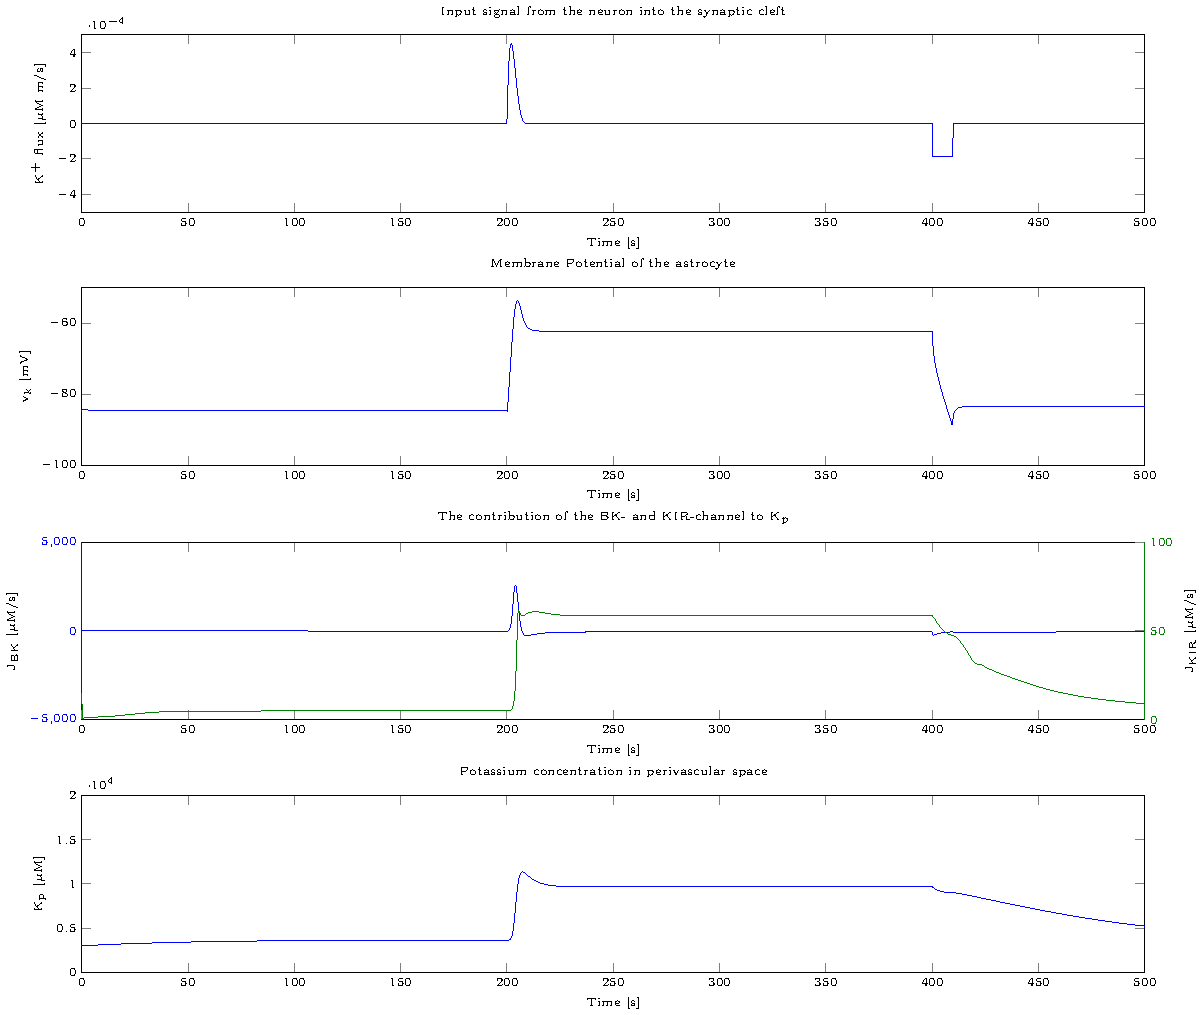
\includegraphics{figures/1_Input_signal.pdf}
			\caption{The input signal}
			\label{fig:1IS}
		\end{figure}
		
		\begin{figure}[h!]
			\centering
			\tiny 
			\setlength\figureheight{3 cm} 
			\setlength\figurewidth{9 cm}
			%% % This file was created by matlab2tikz v0.3.3.
% Copyright (c) 2008--2013, Nico Schlömer <nico.schloemer@gmail.com>
% All rights reserved.
% 
% The latest updates can be retrieved from
%   http://www.mathworks.com/matlabcentral/fileexchange/22022-matlab2tikz
% where you can also make suggestions and rate matlab2tikz.
% 
% 
% 
\tiny 
\newlength\figureheight 
\newlength\figurewidth 
\setlength\figureheight{3 cm} 
\setlength\figurewidth{9 cm}
\begin{tikzpicture}

\begin{axis}[%
width=\figurewidth,
height=\figureheight,
scale only axis,
xmin=0,
xmax=500,
xlabel={Time [s]},
ymin=0,
ymax=0.4,
ylabel={$\text{[IP3] [}\mu\text{M]}$},
name=plot3,
title={Astrocyte IP3 concentration}
]
\addplot [
color=blue,
solid,
forget plot
]
table[row sep=crcr]{
0 1e-05\\
0.0011996 8.23181293851022e-05\\
0.0023992 0.000154530594151028\\
0.0035988 0.000226635321100999\\
0.0085566 0.000523575165494511\\
0.013514 0.000818723541712303\\
0.018472 0.00111206106034376\\
0.02343 0.00140358829926914\\
0.033542 0.00199264015476282\\
0.043655 0.00257428644079317\\
0.053767 0.00314862365114293\\
0.063879 0.00371574715531397\\
0.073991 0.00427574822845227\\
0.084819 0.00486757975592366\\
0.095647 0.00545145494450221\\
0.10647 0.006027480635512\\
0.1173 0.00659576241429792\\
0.12813 0.0071564044438324\\
0.14659 0.0080948319221855\\
0.16505 0.00901185442718942\\
0.18351 0.00990796062193103\\
0.20197 0.0107836275916982\\
0.22042 0.011639321418772\\
0.26398 0.0135817212000039\\
0.30753 0.0154211911870018\\
0.35108 0.0171632014330779\\
0.37397 0.018041571999227\\
0.38969 0.0186299866092517\\
0.4054 0.0192069558539047\\
0.42111 0.019772703758594\\
0.43393 0.020226485029915\\
0.44676 0.0206730479697069\\
0.45959 0.0211125072616507\\
0.47242 0.0215449758488828\\
0.48525 0.0219705649418226\\
0.50035 0.0224627631373495\\
0.51544 0.0229457599091073\\
0.53054 0.0234197273233477\\
0.54564 0.0238848341692237\\
0.56073 0.0243412460720981\\
0.57728 0.0248315384029803\\
0.59382 0.0253117971398671\\
0.61036 0.0257822275128697\\
0.6269 0.026243030585003\\
0.64344 0.0266944033749434\\
0.65998 0.0271365388939442\\
0.69992 0.0281670303894694\\
0.73986 0.0291473373729467\\
0.77979 0.0300799105102768\\
0.81973 0.0309670752356413\\
0.85967 0.0318110412465532\\
0.99616 0.0344078620280908\\
1.1327 0.0365978433310239\\
1.2692 0.038442215025675\\
1.4056 0.0399954574228418\\
1.6062 0.0418379790761354\\
1.8067 0.043267792177813\\
2.0072 0.0443806919561372\\
2.2078 0.0452480805364043\\
2.4083 0.0459238872957761\\
2.8551 0.0469237802853968\\
3.302 0.0474955881101372\\
3.7488 0.0478323991026374\\
4.1956 0.048031978932176\\
4.6425 0.048147562515791\\
5.3586 0.0482320235850345\\
6.0748 0.0482669276194201\\
6.791 0.0482851431177013\\
7.5072 0.048294608243271\\
8.2234 0.0482981682499052\\
9.2234 0.0482987784182718\\
10.223 0.0482985618703277\\
11.223 0.048298793721783\\
12.223 0.0482990891131554\\
12.523 0.0482991082855667\\
12.823 0.0482990935352717\\
13.123 0.0482990743904533\\
13.423 0.0482990631703931\\
13.513 0.0482990618705122\\
13.603 0.0482990605522743\\
13.693 0.0482990592099435\\
13.783 0.0482990579639656\\
13.873 0.0482990568669661\\
13.929 0.0482990562643407\\
13.948 0.048299056068132\\
13.967 0.0482990558760074\\
13.986 0.0482990556881837\\
14.004 0.0482990555047591\\
14.023 0.0482990553256664\\
14.079 0.0482990548272558\\
14.134 0.0482990543621077\\
14.189 0.0482990539279412\\
14.244 0.0482990535226728\\
14.299 0.0482990531443858\\
14.354 0.0482990527912927\\
14.409 0.0482990524617185\\
14.465 0.0482990521540961\\
14.52 0.0482990518655878\\
14.575 0.0482990515963867\\
14.631 0.0482990513452008\\
14.686 0.0482990511108246\\
14.742 0.0482990508921333\\
14.811 0.0482990506386868\\
14.88 0.0482990504063082\\
14.95 0.0482990501932428\\
15.019 0.0482990499978859\\
15.089 0.0482990498187667\\
15.202 0.0482990495586491\\
15.315 0.0482990493327941\\
15.428 0.0482990491366603\\
15.541 0.0482990489663357\\
15.654 0.048299048818432\\
15.804 0.0482990486514921\\
15.954 0.0482990485131384\\
16.104 0.0482990483984445\\
16.255 0.0482990483033658\\
16.405 0.0482990482245576\\
16.675 0.0482990481155159\\
16.946 0.0482990480377646\\
17.216 0.0482990479821248\\
17.487 0.0482990479422959\\
17.757 0.0482990479138399\\
18.061 0.0482990478914553\\
18.364 0.0482990478761493\\
18.667 0.0482990478656986\\
18.971 0.0482990478585502\\
19.274 0.0482990478536484\\
19.375 0.0482990478523726\\
19.476 0.0482990478512539\\
19.576 0.0482990478502718\\
19.677 0.0482990478494067\\
19.778 0.0482990478486435\\
19.938 0.0482990478476151\\
20.097 0.0482990478467723\\
20.257 0.0482990478460818\\
20.416 0.0482990478455161\\
20.576 0.0482990478450526\\
20.994 0.0482990478441703\\
21.411 0.0482990478436528\\
21.828 0.0482990478433561\\
22.056 0.048299047843257\\
22.119 0.0482990478432342\\
22.183 0.0482990478432128\\
22.247 0.0482990478431929\\
22.31 0.0482990478431745\\
22.432 0.0482990478431432\\
22.554 0.0482990478431163\\
22.676 0.0482990478430932\\
22.798 0.0482990478430734\\
22.92 0.0482990478430564\\
23.367 0.0482990478430104\\
23.684 0.048299047842991\\
24 0.0482990478429783\\
24.242 0.0482990478429716\\
24.484 0.0482990478429667\\
24.726 0.048299047842963\\
24.968 0.0482990478429603\\
25.298 0.0482990478429578\\
25.628 0.0482990478429561\\
25.958 0.048299047842955\\
26.288 0.0482990478429543\\
26.618 0.0482990478429538\\
27.087 0.0482990478429534\\
27.556 0.0482990478429532\\
28.025 0.048299047842953\\
28.494 0.0482990478429529\\
28.964 0.0482990478429529\\
29.615 0.0482990478429529\\
30.266 0.0482990478429529\\
30.917 0.0482990478429529\\
31.569 0.0482990478429529\\
32.372 0.0482990478429529\\
33.175 0.0482990478429529\\
33.979 0.0482990478429529\\
34.782 0.0482990478429529\\
35.586 0.0482990478429529\\
36.23 0.0482990478429529\\
36.875 0.0482990478429529\\
37.52 0.0482990478429529\\
38.164 0.0482990478429529\\
38.969 0.0482990478429529\\
39.774 0.0482990478429529\\
40.579 0.0482990478429529\\
41.384 0.0482990478429529\\
42.189 0.0482990478429529\\
43.189 0.0482990478429529\\
44.189 0.0482990478429529\\
45.189 0.0482990478429529\\
46.189 0.0482990478429529\\
47.189 0.0482990478429529\\
48.189 0.0482990478429529\\
49.189 0.0482990478429529\\
50.189 0.0482990478429529\\
51.189 0.0482990478429529\\
52.189 0.0482990478429529\\
53.189 0.0482990478429529\\
54.189 0.0482990478429529\\
55.189 0.0482990478429529\\
56.189 0.0482990478429529\\
57.189 0.0482990478429529\\
58.189 0.0482990478429529\\
59.189 0.0482990478429529\\
60.189 0.0482990478429529\\
61.189 0.0482990478429529\\
62.189 0.0482990478429529\\
63.189 0.0482990478429529\\
64.189 0.0482990478429529\\
65.189 0.0482990478429529\\
66.189 0.0482990478429529\\
67.189 0.0482990478429529\\
68.189 0.0482990478429529\\
69.189 0.0482990478429529\\
70.189 0.0482990478429529\\
71.189 0.0482990478429529\\
72.189 0.0482990478429529\\
73.189 0.0482990478429529\\
74.189 0.0482990478429529\\
75.189 0.0482990478429529\\
76.189 0.0482990478429529\\
77.189 0.0482990478429529\\
78.189 0.0482990478429529\\
79.189 0.0482990478429529\\
80.189 0.0482990478429529\\
81.189 0.0482990478429529\\
82.189 0.0482990478429529\\
83.189 0.0482990478429529\\
84.189 0.0482990478429529\\
85.189 0.0482990478429529\\
86.189 0.0482990478429529\\
87.189 0.0482990478429529\\
88.189 0.0482990478429529\\
89.189 0.0482990478429529\\
90.189 0.0482990478429529\\
91.189 0.0482990478429529\\
92.189 0.0482990478429529\\
93.189 0.0482990478429529\\
94.189 0.0482990478429529\\
95.189 0.0482990478429529\\
96.189 0.0482990478429529\\
97.189 0.0482990478429529\\
98.189 0.0482990478429529\\
99.189 0.0482990478429529\\
100.19 0.0482990478429529\\
101.19 0.0482990478429529\\
102.19 0.0482990478429529\\
103.19 0.0482990478429529\\
104.19 0.0482990478429529\\
105.19 0.0482990478429529\\
106.19 0.0482990478429529\\
107.19 0.0482990478429529\\
108.19 0.0482990478429529\\
109.19 0.0482990478429529\\
110.19 0.0482990478429529\\
111.19 0.0482990478429529\\
112.19 0.0482990478429529\\
113.19 0.0482990478429529\\
114.19 0.0482990478429529\\
115.19 0.0482990478429529\\
116.19 0.0482990478429529\\
117.19 0.0482990478429529\\
118.19 0.0482990478429529\\
119.19 0.0482990478429529\\
120.19 0.0482990478429529\\
121.19 0.0482990478429529\\
122.19 0.0482990478429529\\
123.19 0.0482990478429529\\
124.19 0.0482990478429529\\
125.19 0.0482990478429529\\
126.19 0.0482990478429529\\
127.19 0.0482990478429529\\
128.19 0.0482990478429529\\
129.19 0.0482990478429529\\
130.19 0.0482990478429529\\
131.19 0.0482990478429529\\
132.19 0.0482990478429529\\
133.19 0.0482990478429529\\
134.19 0.0482990478429529\\
135.19 0.0482990478429529\\
136.19 0.0482990478429529\\
137.19 0.0482990478429529\\
138.19 0.0482990478429529\\
139.19 0.0482990478429529\\
140.19 0.0482990478429529\\
141.19 0.0482990478429529\\
142.19 0.0482990478429529\\
143.19 0.0482990478429529\\
144.19 0.0482990478429529\\
145.19 0.0482990478429529\\
146.19 0.0482990478429529\\
147.19 0.0482990478429529\\
148.19 0.0482990478429529\\
149.19 0.0482990478429529\\
150.19 0.0482990478429529\\
151.19 0.0482990478429529\\
152.19 0.0482990478429529\\
153.19 0.0482990478429529\\
154.19 0.0482990478429529\\
155.19 0.0482990478429529\\
156.19 0.0482990478429529\\
157.19 0.0482990478429529\\
158.19 0.0482990478429529\\
159.19 0.0482990478429529\\
160.19 0.0482990478429529\\
161.19 0.0482990478429529\\
162.19 0.0482990478429529\\
163.19 0.0482990478429529\\
164.19 0.0482990478429529\\
165.19 0.0482990478429529\\
166.19 0.0482990478429529\\
167.19 0.0482990478429529\\
168.19 0.0482990478429529\\
169.19 0.0482990478429529\\
170.19 0.0482990478429529\\
171.19 0.0482990478429529\\
172.19 0.0482990478429529\\
173.19 0.0482990478429529\\
174.19 0.0482990478429529\\
175.19 0.0482990478429529\\
176.19 0.0482990478429529\\
177.19 0.0482990478429529\\
178.19 0.0482990478429529\\
179.19 0.0482990478429529\\
180.19 0.0482990478429529\\
181.19 0.0482990478429529\\
182.19 0.0482990478429529\\
183.19 0.0482990478429532\\
184.19 0.0482990478429555\\
185.19 0.0482990478429722\\
186.19 0.0482990478430954\\
187.19 0.0482990478440062\\
188.19 0.0482990478507362\\
189.19 0.0482990479004644\\
190.19 0.0482990482679086\\
191.19 0.0482990509829745\\
192.19 0.0482990710447452\\
193.19 0.0482992192821187\\
194.19 0.0483003146067703\\
195.19 0.0483084074971951\\
196.19 0.048368177668618\\
196.81 0.0485129160404505\\
197.25 0.0487832240899059\\
197.57 0.0491800570909175\\
197.82 0.0497157785949221\\
198.03 0.0503859954240403\\
198.24 0.0513964419332711\\
198.38 0.0523221344009247\\
198.52 0.0535404413501772\\
198.63 0.0547404032738453\\
198.74 0.0562186956874274\\
198.83 0.0576584710289503\\
198.92 0.0593541276541005\\
199.01 0.0613406643627219\\
199.17 0.0652992023724666\\
199.32 0.0702875285867363\\
199.47 0.0765087673040735\\
199.62 0.0841105699354715\\
199.84 0.0978012890697069\\
200.07 0.114414716627266\\
200.29 0.133302825788456\\
200.51 0.153396272874484\\
200.69 0.169890234017051\\
200.87 0.185745761486845\\
201.05 0.200501732623423\\
201.23 0.213870938826959\\
201.42 0.225719071133013\\
201.6 0.236188795143947\\
201.79 0.24514206228065\\
201.97 0.252704017967436\\
202.15 0.259026911353744\\
202.34 0.264270520473413\\
202.63 0.270700718104186\\
202.92 0.275375962273122\\
203.21 0.278744132919803\\
203.5 0.281154685602475\\
203.79 0.282870633669065\\
204.09 0.284123257907662\\
204.39 0.28499614030335\\
204.69 0.285602813887014\\
204.94 0.285960473673439\\
205.19 0.286224519602106\\
205.44 0.286418949372314\\
205.68 0.286563263841964\\
205.85 0.286638967937237\\
206.02 0.286700508060142\\
206.19 0.286750437437116\\
206.36 0.286790883624207\\
206.6 0.286835849679757\\
206.84 0.286869050674571\\
207.08 0.286893516787062\\
207.32 0.286911549120576\\
207.65 0.286928754384964\\
207.99 0.286940013116891\\
208.32 0.286947483759322\\
208.65 0.286952466004113\\
208.99 0.286955773045591\\
209.66 0.286959228410187\\
210.18 0.286960581483872\\
210.7 0.286961358732073\\
211.22 0.286961773943293\\
211.74 0.286961976464479\\
212.26 0.286962073376792\\
212.9 0.286962128517047\\
213.54 0.286962158210409\\
214.18 0.286962175204127\\
214.82 0.286962182986482\\
215.46 0.286962185380389\\
216.16 0.286962185846926\\
216.87 0.286962186092799\\
217.57 0.286962186427987\\
218.27 0.286962186645601\\
218.98 0.286962186693766\\
219.98 0.28696218666597\\
220.98 0.286962186639302\\
221.98 0.286962186646069\\
222.98 0.286962186659682\\
223.98 0.28696218666339\\
224.98 0.286962186661839\\
225.98 0.286962186660016\\
226.98 0.286962186659197\\
227.98 0.286962186659031\\
228.98 0.286962186659066\\
229.98 0.286962186659104\\
230.98 0.28696218665911\\
231.98 0.286962186659107\\
232.98 0.286962186659108\\
233.98 0.286962186659112\\
234.98 0.286962186659113\\
235.98 0.286962186659114\\
236.98 0.286962186659114\\
237.98 0.286962186659113\\
238.98 0.286962186659113\\
239.98 0.286962186659113\\
240.98 0.286962186659113\\
241.98 0.286962186659113\\
242.98 0.286962186659113\\
243.98 0.286962186659113\\
244.98 0.286962186659113\\
245.98 0.286962186659113\\
246.98 0.286962186659113\\
247.98 0.286962186659113\\
248.98 0.286962186659113\\
249.98 0.286962186659113\\
250.98 0.286962186659113\\
251.98 0.286962186659113\\
252.98 0.286962186659113\\
253.98 0.286962186659113\\
254.98 0.286962186659113\\
255.98 0.286962186659113\\
256.98 0.286962186659113\\
257.98 0.286962186659113\\
258.98 0.286962186659113\\
259.98 0.286962186659113\\
260.98 0.286962186659113\\
261.98 0.286962186659113\\
262.98 0.286962186659113\\
263.98 0.286962186659113\\
264.98 0.286962186659113\\
265.98 0.286962186659113\\
266.98 0.286962186659113\\
267.98 0.286962186659113\\
268.98 0.286962186659113\\
269.98 0.286962186659113\\
270.98 0.286962186659113\\
271.98 0.286962186659113\\
272.98 0.286962186659113\\
273.98 0.286962186659113\\
274.98 0.286962186659113\\
275.98 0.286962186659113\\
276.98 0.286962186659113\\
277.98 0.286962186659113\\
278.98 0.286962186659113\\
279.98 0.286962186659113\\
280.98 0.286962186659113\\
281.98 0.286962186659113\\
282.98 0.286962186659113\\
283.98 0.286962186659113\\
284.98 0.286962186659113\\
285.98 0.286962186659113\\
286.98 0.286962186659113\\
287.98 0.286962186659113\\
288.98 0.286962186659113\\
289.98 0.286962186659113\\
290.98 0.286962186659113\\
291.98 0.286962186659113\\
292.98 0.286962186659113\\
293.98 0.286962186659113\\
294.98 0.286962186659113\\
295.98 0.286962186659113\\
296.98 0.286962186659113\\
297.98 0.286962186659113\\
298.98 0.286962186659113\\
299.98 0.286962186659113\\
300.98 0.286962186659113\\
301.98 0.286962186659113\\
302.98 0.286962186659113\\
303.98 0.286962186659113\\
304.98 0.286962186659113\\
305.98 0.286962186659113\\
306.98 0.286962186659113\\
307.98 0.286962186659113\\
308.98 0.286962186659113\\
309.98 0.286962186659113\\
310.98 0.286962186659113\\
311.98 0.286962186659113\\
312.98 0.286962186659113\\
313.98 0.286962186659113\\
314.98 0.286962186659113\\
315.98 0.286962186659113\\
316.98 0.286962186659113\\
317.98 0.286962186659113\\
318.98 0.286962186659113\\
319.98 0.286962186659113\\
320.98 0.286962186659113\\
321.98 0.286962186659113\\
322.98 0.286962186659113\\
323.98 0.286962186659113\\
324.98 0.286962186659113\\
325.98 0.286962186659113\\
326.98 0.286962186659113\\
327.98 0.286962186659113\\
328.98 0.286962186659113\\
329.98 0.286962186659113\\
330.98 0.286962186659113\\
331.98 0.286962186659113\\
332.98 0.286962186659113\\
333.98 0.286962186659113\\
334.98 0.286962186659113\\
335.98 0.286962186659113\\
336.98 0.286962186659113\\
337.98 0.286962186659113\\
338.98 0.286962186659113\\
339.98 0.286962186659113\\
340.98 0.286962186659113\\
341.98 0.286962186659113\\
342.98 0.286962186659113\\
343.98 0.286962186659113\\
344.98 0.286962186659113\\
345.98 0.286962186659113\\
346.98 0.286962186659113\\
347.98 0.286962186659113\\
348.98 0.286962186659113\\
349.98 0.286962186659113\\
350.98 0.286962186659113\\
351.98 0.286962186659113\\
352.98 0.286962186659113\\
353.98 0.286962186659113\\
354.98 0.286962186659113\\
355.98 0.286962186659113\\
356.98 0.286962186659113\\
357.98 0.286962186659113\\
358.98 0.286962186659113\\
359.98 0.286962186659113\\
360.98 0.286962186659113\\
361.98 0.286962186659113\\
362.98 0.286962186659113\\
363.98 0.286962186659113\\
364.98 0.286962186659113\\
365.98 0.286962186659113\\
366.98 0.286962186659113\\
367.98 0.286962186659113\\
368.98 0.286962186659113\\
369.98 0.286962186659113\\
370.98 0.286962186659113\\
371.98 0.286962186659113\\
372.98 0.286962186659113\\
373.98 0.286962186659113\\
374.98 0.286962186659113\\
375.98 0.286962186659113\\
376.98 0.286962186659113\\
377.98 0.286962186659113\\
378.98 0.286962186659113\\
379.98 0.286962186659113\\
380.98 0.286962186659113\\
381.98 0.286962186659113\\
382.98 0.286962186659113\\
383.98 0.286962186659112\\
384.98 0.286962186659102\\
385.98 0.286962186659032\\
386.98 0.286962186658509\\
387.98 0.286962186654648\\
388.98 0.286962186626117\\
389.98 0.286962186415298\\
390.98 0.28696218485755\\
391.98 0.286962173347258\\
392.98 0.286962088297128\\
393.98 0.28696145986011\\
394.98 0.286956816476557\\
395.98 0.286922515688375\\
396.98 0.286669579160103\\
397.98 0.284828229455401\\
398.44 0.282362869540958\\
398.8 0.278279348366678\\
399.07 0.272945122510641\\
399.35 0.264474066798662\\
399.55 0.255952332800874\\
399.76 0.244921212645399\\
399.96 0.231375103626877\\
400.26 0.208508132916841\\
400.34 0.200964076095383\\
400.43 0.193222325363408\\
400.52 0.185351799693633\\
400.61 0.177428592279432\\
400.92 0.150138816344732\\
401.24 0.125619948250085\\
401.56 0.105178565436288\\
401.87 0.0891299099321024\\
402.11 0.07967631869913\\
402.35 0.0722316763635949\\
402.59 0.0664433757881965\\
402.83 0.0619875629444928\\
403.14 0.0577733063376611\\
403.45 0.0548439114067887\\
403.77 0.0528087168702512\\
404.08 0.0513955055553779\\
404.39 0.0504181887586273\\
404.93 0.0494119850894662\\
405.47 0.048890619608861\\
406.02 0.0486079403435351\\
406.56 0.0484543117235023\\
407.1 0.0483752526299002\\
408.1 0.0483298639591269\\
408.77 0.0483133331183441\\
409.43 0.0483036427884534\\
410.1 0.048299969232246\\
410.61 0.0482994878555999\\
411.12 0.0482994481935458\\
411.63 0.0482993362458038\\
412.15 0.0482991810039785\\
412.66 0.0482990839755733\\
413.31 0.0482990452168889\\
413.95 0.0482990518046773\\
414.6 0.0482990580143603\\
415.25 0.0482990547204634\\
415.9 0.0482990494273501\\
416.77 0.048299046175962\\
417.65 0.0482990469345985\\
418.52 0.0482990481400006\\
419.4 0.048299048315306\\
420.28 0.0482990479690126\\
421.2 0.0482990477730461\\
422.12 0.0482990478542363\\
423.04 0.0482990479277687\\
423.96 0.0482990478835708\\
424.89 0.0482990478235823\\
425.81 0.0482990478218365\\
426.73 0.0482990478470605\\
427.68 0.0482990478564499\\
428.64 0.0482990478495799\\
429.59 0.0482990478424929\\
430.55 0.048299047841199\\
431.5 0.0482990478426251\\
432.5 0.0482990478434994\\
433.5 0.0482990478432943\\
434.5 0.0482990478429148\\
435.5 0.0482990478428302\\
436.5 0.0482990478429178\\
437.5 0.0482990478429781\\
438.5 0.0482990478429733\\
439.5 0.0482990478429597\\
440.5 0.0482990478429532\\
441.5 0.0482990478429519\\
442.5 0.0482990478429524\\
443.5 0.0482990478429526\\
444.5 0.0482990478429528\\
445.5 0.0482990478429528\\
446.5 0.0482990478429528\\
447.5 0.0482990478429529\\
448.5 0.0482990478429529\\
449.5 0.0482990478429529\\
450.5 0.0482990478429529\\
451.5 0.0482990478429529\\
452.5 0.0482990478429529\\
453.5 0.0482990478429529\\
454.5 0.0482990478429529\\
455.5 0.0482990478429529\\
456.5 0.0482990478429529\\
457.5 0.0482990478429529\\
458.5 0.0482990478429529\\
459.5 0.0482990478429529\\
460.5 0.0482990478429529\\
461.5 0.0482990478429529\\
462.5 0.0482990478429529\\
463.5 0.0482990478429529\\
464.5 0.0482990478429529\\
465.5 0.0482990478429529\\
466.5 0.0482990478429529\\
467.5 0.0482990478429529\\
468.5 0.0482990478429529\\
469.5 0.0482990478429529\\
470.5 0.0482990478429529\\
471.5 0.0482990478429529\\
472.5 0.0482990478429529\\
473.5 0.0482990478429529\\
474.5 0.0482990478429529\\
475.5 0.0482990478429529\\
476.5 0.0482990478429529\\
477.5 0.0482990478429529\\
478.5 0.0482990478429529\\
479.5 0.0482990478429529\\
480.5 0.0482990478429529\\
481.5 0.0482990478429529\\
482.5 0.0482990478429529\\
483.5 0.0482990478429529\\
484.5 0.0482990478429529\\
485.5 0.0482990478429529\\
486.5 0.0482990478429529\\
487.5 0.0482990478429529\\
488.5 0.0482990478429529\\
489.5 0.0482990478429529\\
490.5 0.0482990478429529\\
491.5 0.0482990478429529\\
492.5 0.0482990478429529\\
493.5 0.0482990478429529\\
494.5 0.0482990478429529\\
495.5 0.0482990478429529\\
496.5 0.0482990478429529\\
497.5 0.0482990478429529\\
498.5 0.0482990478429529\\
499.5 0.0482990478429529\\
500 0.0482990478429529\\
};
\end{axis}

\begin{axis}[%
width=\figurewidth,
height=\figureheight,
scale only axis,
xmin=0,
xmax=500,
xlabel={Time [s]},
ymin=0.0055,
ymax=0.0075,
ylabel={$\text{[K] [}\mu\text{M]}$},
name=plot1,
at=(plot3.above north west),
anchor=below south west,
title={Astrocyte Potassium concentration}
]
\addplot [
color=blue,
solid,
forget plot
]
table[row sep=crcr]{
0 0.00552782\\
0.0011996 0.00552778386850785\\
0.0023992 0.00552774844521066\\
0.0035988 0.00552771378402968\\
0.0085566 0.00552757758552962\\
0.013514 0.00552745281903946\\
0.018472 0.00552733874173648\\
0.02343 0.00552723450426542\\
0.033542 0.00552704915277388\\
0.043655 0.00552689515210781\\
0.053767 0.00552676712846656\\
0.063879 0.00552666071765313\\
0.073991 0.00552657236182217\\
0.084819 0.00552649444388304\\
0.095647 0.00552643081724898\\
0.10647 0.00552637897586548\\
0.1173 0.00552633685953153\\
0.12813 0.00552630277151443\\
0.14659 0.0055262594647252\\
0.16505 0.00552623008270239\\
0.18351 0.00552621065826982\\
0.20197 0.00552619842874652\\
0.22042 0.00552619141732001\\
0.26398 0.00552618871513652\\
0.30753 0.00552619546593947\\
0.35108 0.00552620588015998\\
0.37397 0.00552621194497686\\
0.38969 0.00552621644919601\\
0.4054 0.0055262211303168\\
0.42111 0.00552622588787156\\
0.43393 0.00552622978965645\\
0.44676 0.00552623369860262\\
0.45959 0.00552623761011133\\
0.47242 0.00552624151794393\\
0.48525 0.00552624541557395\\
0.50035 0.0055262499825447\\
0.51544 0.00552625452200598\\
0.53054 0.00552625902962251\\
0.54564 0.00552626350223534\\
0.56073 0.00552626793745453\\
0.57728 0.00552627275197829\\
0.59382 0.00552627751777579\\
0.61036 0.00552628223375309\\
0.6269 0.00552628689921634\\
0.64344 0.00552629151375819\\
0.65998 0.00552629607719394\\
0.69992 0.0055263068844632\\
0.73986 0.0055263173964076\\
0.77979 0.00552632761766088\\
0.81973 0.00552633755427015\\
0.85967 0.00552634721273489\\
0.99616 0.00552637825263795\\
1.1327 0.0055264063871857\\
1.2692 0.00552643185909895\\
1.4056 0.00552645490642631\\
1.6062 0.00552648480197139\\
1.8067 0.00552651056330957\\
2.0072 0.00552653277509924\\
2.2078 0.00552655193405194\\
2.4083 0.00552656845866666\\
2.8551 0.00552659746365014\\
3.302 0.00552661830176859\\
3.7488 0.00552663333274674\\
4.1956 0.00552664418615071\\
4.6425 0.00552665201130502\\
5.3586 0.00552666013740774\\
6.0748 0.00552666494769064\\
6.791 0.0055266678529035\\
7.5072 0.00552666960901946\\
8.2234 0.00552667065266435\\
9.2234 0.00552667140393521\\
10.223 0.00552667176600272\\
11.223 0.00552667195661559\\
12.223 0.0055266720573189\\
12.523 0.0055266720767457\\
12.823 0.00552667209037987\\
13.123 0.00552667210040352\\
13.423 0.00552667210841547\\
13.513 0.00552667211058813\\
13.603 0.00552667211262199\\
13.693 0.00552667211451909\\
13.783 0.00552667211629231\\
13.873 0.00552667211795368\\
13.929 0.00552667211892559\\
13.948 0.00552667211924846\\
13.967 0.00552667211956669\\
13.986 0.00552667211988008\\
14.004 0.00552667212018836\\
14.023 0.00552667212049134\\
14.079 0.00552667212134307\\
14.134 0.00552667212214802\\
14.189 0.00552667212291327\\
14.244 0.00552667212366365\\
14.299 0.00552667212444205\\
14.354 0.00552667212526214\\
14.409 0.0055266721260613\\
14.465 0.00552667212673799\\
14.52 0.00552667212723518\\
14.575 0.00552667212756098\\
14.631 0.00552667212776502\\
14.686 0.00552667212789398\\
14.742 0.00552667212798186\\
14.811 0.00552667212808079\\
14.88 0.00552667212822227\\
14.95 0.00552667212845021\\
15.019 0.00552667212878227\\
15.089 0.00552667212921153\\
15.202 0.00552667213006095\\
15.315 0.00552667213102042\\
15.428 0.0055266721320073\\
15.541 0.00552667213296482\\
15.654 0.00552667213386219\\
15.804 0.00552667213494033\\
15.954 0.00552667213586969\\
16.104 0.0055266721366448\\
16.255 0.00552667213726671\\
16.405 0.00552667213774739\\
16.675 0.00552667213838112\\
16.946 0.00552667213892031\\
17.216 0.00552667213950829\\
17.487 0.00552667214008745\\
17.757 0.00552667214056657\\
18.061 0.00552667214098606\\
18.364 0.00552667214132812\\
18.667 0.00552667214160599\\
18.971 0.00552667214182436\\
19.274 0.0055266721419974\\
19.375 0.00552667214204732\\
19.476 0.00552667214209309\\
19.576 0.00552667214213408\\
19.677 0.00552667214217061\\
19.778 0.00552667214220369\\
19.938 0.00552667214225123\\
20.097 0.00552667214229405\\
20.257 0.00552667214233338\\
20.416 0.00552667214236953\\
20.576 0.00552667214240254\\
20.994 0.00552667214247685\\
21.411 0.00552667214253745\\
21.828 0.00552667214258816\\
22.056 0.00552667214261247\\
22.119 0.0055266721426188\\
22.183 0.00552667214262467\\
22.247 0.00552667214262979\\
22.31 0.0055266721426341\\
22.432 0.00552667214264033\\
22.554 0.00552667214264472\\
22.676 0.00552667214264785\\
22.798 0.00552667214264998\\
22.92 0.00552667214265102\\
23.367 0.00552667214264787\\
23.684 0.00552667214264038\\
24 0.00552667214263073\\
24.242 0.0055266721426231\\
24.484 0.00552667214261662\\
24.726 0.00552667214261241\\
24.968 0.00552667214261141\\
25.298 0.00552667214261625\\
25.628 0.00552667214262886\\
25.958 0.00552667214264889\\
26.288 0.00552667214267503\\
26.618 0.00552667214270546\\
27.087 0.0055266721427525\\
27.556 0.00552667214280009\\
28.025 0.00552667214284538\\
28.494 0.00552667214288696\\
28.964 0.00552667214292441\\
29.615 0.00552667214296982\\
30.266 0.00552667214300856\\
30.917 0.00552667214304194\\
31.569 0.00552667214307141\\
32.372 0.00552667214310473\\
33.175 0.00552667214313723\\
33.979 0.00552667214317161\\
34.782 0.00552667214320926\\
35.586 0.0055266721432498\\
36.23 0.00552667214328325\\
36.875 0.00552667214331691\\
37.52 0.00552667214335013\\
38.164 0.00552667214338248\\
38.969 0.00552667214342129\\
39.774 0.00552667214345865\\
40.579 0.0055266721434948\\
41.384 0.0055266721435301\\
42.189 0.00552667214356496\\
43.189 0.00552667214360786\\
44.189 0.00552667214365036\\
45.189 0.00552667214369222\\
46.189 0.00552667214373306\\
47.189 0.00552667214377269\\
48.189 0.00552667214381108\\
49.189 0.00552667214384834\\
50.189 0.00552667214388451\\
51.189 0.00552667214391967\\
52.189 0.0055266721439539\\
53.189 0.00552667214398722\\
54.189 0.00552667214401964\\
55.189 0.00552667214405119\\
56.189 0.00552667214408189\\
57.189 0.00552667214411177\\
58.189 0.00552667214414099\\
59.189 0.00552667214416959\\
60.189 0.00552667214419763\\
61.189 0.00552667214422488\\
62.189 0.00552667214425167\\
63.189 0.00552667214427788\\
64.189 0.00552667214430349\\
65.189 0.00552667214432854\\
66.189 0.00552667214435305\\
67.189 0.00552667214437702\\
68.189 0.0055266721444005\\
69.189 0.00552667214442334\\
70.189 0.00552667214444564\\
71.189 0.00552667214446744\\
72.189 0.00552667214448884\\
73.189 0.00552667214450976\\
74.189 0.00552667214453024\\
75.189 0.00552667214455025\\
76.189 0.00552667214456969\\
77.189 0.00552667214458865\\
78.189 0.00552667214460716\\
79.189 0.00552667214462525\\
80.189 0.00552667214464292\\
81.189 0.00552667214465993\\
82.189 0.00552667214467702\\
83.189 0.00552667214469365\\
84.189 0.0055266721447099\\
85.189 0.00552667214472578\\
86.189 0.0055266721447412\\
87.189 0.00552667214475603\\
88.189 0.0055266721447707\\
89.189 0.00552667214478508\\
90.189 0.00552667214479915\\
91.189 0.00552667214481292\\
92.189 0.00552667214482639\\
93.189 0.00552667214483958\\
94.189 0.00552667214485247\\
95.189 0.00552667214486509\\
96.189 0.00552667214487743\\
97.189 0.00552667214488951\\
98.189 0.00552667214490132\\
99.189 0.00552667214491287\\
100.19 0.00552667214492417\\
101.19 0.00552667214493523\\
102.19 0.00552667214494604\\
103.19 0.00552667214495662\\
104.19 0.00552667214496712\\
105.19 0.00552667214497713\\
106.19 0.005526672144987\\
107.19 0.00552667214499668\\
108.19 0.00552667214500614\\
109.19 0.00552667214501541\\
110.19 0.00552667214502447\\
111.19 0.00552667214503334\\
112.19 0.00552667214504201\\
113.19 0.0055266721450505\\
114.19 0.0055266721450588\\
115.19 0.00552667214506693\\
116.19 0.00552667214507488\\
117.19 0.00552667214508265\\
118.19 0.00552667214509027\\
119.19 0.00552667214509771\\
120.19 0.005526672145105\\
121.19 0.00552667214511213\\
122.19 0.00552667214511911\\
123.19 0.00552667214512604\\
124.19 0.00552667214513265\\
125.19 0.00552667214513917\\
126.19 0.00552667214514556\\
127.19 0.00552667214515182\\
128.19 0.00552667214515795\\
129.19 0.00552667214516394\\
130.19 0.00552667214516981\\
131.19 0.00552667214517556\\
132.19 0.00552667214518118\\
133.19 0.00552667214518668\\
134.19 0.00552667214519206\\
135.19 0.00552667214519733\\
136.19 0.00552667214520248\\
137.19 0.00552667214520753\\
138.19 0.00552667214521247\\
139.19 0.0055266721452173\\
140.19 0.00552667214522203\\
141.19 0.00552667214522666\\
142.19 0.00552667214523119\\
143.19 0.00552667214523563\\
144.19 0.00552667214523997\\
145.19 0.00552667214524422\\
146.19 0.00552667214524837\\
147.19 0.00552667214525245\\
148.19 0.00552667214525643\\
149.19 0.00552667214526033\\
150.19 0.00552667214526415\\
151.19 0.00552667214526788\\
152.19 0.00552667214527154\\
153.19 0.00552667214527512\\
154.19 0.00552667214527862\\
155.19 0.00552667214528206\\
156.19 0.00552667214528541\\
157.19 0.00552667214528869\\
158.19 0.00552667214529196\\
159.19 0.00552667214529508\\
160.19 0.00552667214529815\\
161.19 0.00552667214530117\\
162.19 0.00552667214530412\\
163.19 0.00552667214530701\\
164.19 0.00552667214530984\\
165.19 0.0055266721453126\\
166.19 0.00552667214531532\\
167.19 0.00552667214531797\\
168.19 0.00552667214532057\\
169.19 0.00552667214532311\\
170.19 0.0055266721453256\\
171.19 0.00552667214532804\\
172.19 0.00552667214533043\\
173.19 0.00552667214533277\\
174.19 0.00552667214533505\\
175.19 0.00552667214533729\\
176.19 0.00552667214533948\\
177.19 0.00552667214534163\\
178.19 0.00552667214534373\\
179.19 0.00552667214534578\\
180.19 0.0055266721453478\\
181.19 0.00552667214534977\\
182.19 0.00552667214535169\\
183.19 0.00552667214535358\\
184.19 0.00552667214535543\\
185.19 0.00552667214535724\\
186.19 0.00552667214535902\\
187.19 0.00552667214536075\\
188.19 0.00552667214536245\\
189.19 0.00552667214536411\\
190.19 0.00552667214536575\\
191.19 0.00552667214536737\\
192.19 0.00552667214536891\\
193.19 0.00552667214537044\\
194.19 0.00552667214537193\\
195.19 0.00552667214537348\\
196.19 0.00552667214537539\\
196.81 0.00552667214537636\\
197.25 0.00552667214537761\\
197.57 0.00552667214537896\\
197.82 0.00552667214538046\\
198.03 0.00552667214538212\\
198.24 0.00552667214538461\\
198.38 0.00552667214538656\\
198.52 0.00552667214538924\\
198.63 0.00552667214539168\\
198.74 0.00552667214539481\\
198.83 0.00552667214539772\\
198.92 0.00552667214540126\\
199.01 0.00552667214540543\\
199.17 0.00552667214541363\\
199.32 0.00552667214542414\\
199.47 0.00552667214543768\\
199.62 0.00552667214545488\\
199.84 0.00552667214548728\\
200.07 0.00553249053281064\\
200.29 0.0055486385008647\\
200.51 0.00558130479299059\\
200.69 0.00562196529602212\\
200.87 0.00567272540626624\\
201.05 0.00573069332351177\\
201.23 0.00579396766952985\\
201.42 0.00586136336539524\\
201.6 0.00593294617473683\\
201.79 0.00600637270873043\\
201.97 0.00608048807734967\\
202.15 0.00615439526068084\\
202.34 0.00622741967338579\\
202.63 0.00633925381034055\\
202.92 0.00644587908327913\\
203.21 0.0065462175591224\\
203.5 0.00663975882243383\\
203.79 0.00672633074402246\\
204.09 0.00680869349176078\\
204.39 0.00688343748796523\\
204.69 0.00695056100844765\\
204.94 0.00700003035574208\\
205.19 0.00704459151185795\\
205.44 0.00708440922329625\\
205.68 0.00711962670399822\\
205.85 0.00714112521212688\\
206.02 0.00716061738638762\\
206.19 0.00717818928045399\\
206.36 0.00719393631915386\\
206.6 0.00721343418898606\\
206.84 0.00722977345863237\\
207.08 0.00724328955551198\\
207.32 0.00725433071012319\\
207.65 0.00726612583751732\\
207.99 0.00727468927164748\\
208.32 0.00728083486250642\\
208.65 0.00728524221028809\\
208.99 0.00728845051523071\\
209.66 0.00729255680594734\\
210.18 0.00729465235242675\\
210.7 0.00729621269233941\\
211.22 0.00729736026988488\\
211.74 0.00729818453798064\\
212.26 0.00729877649399757\\
212.9 0.00729929315608346\\
213.54 0.00729964918000709\\
214.18 0.0072998917266934\\
214.82 0.00730005607850777\\
215.46 0.00730016963470246\\
216.16 0.00730025479783115\\
216.87 0.00730031051472182\\
217.57 0.00730034632511223\\
218.27 0.00730037027582035\\
218.98 0.00730038503835845\\
219.98 0.00730039923791449\\
220.98 0.0073004087235473\\
221.98 0.00730041332469189\\
222.98 0.00730041555920117\\
223.98 0.00730041662130889\\
224.98 0.00730041704617341\\
225.98 0.00730041737019566\\
226.98 0.00730041768251109\\
227.98 0.00730041780350861\\
228.98 0.00730041781971992\\
229.98 0.0073004178483621\\
230.98 0.00730041789172579\\
231.98 0.00730041789995239\\
232.98 0.00730041791582547\\
233.98 0.00730041791187236\\
234.98 0.00730041789853278\\
235.98 0.00730041790426778\\
236.98 0.00730041788983065\\
237.98 0.00730041790782024\\
238.98 0.00730041790266972\\
239.98 0.00730041789779533\\
240.98 0.00730041789872068\\
241.98 0.00730041789630419\\
242.98 0.00730041789783907\\
243.98 0.00730041789600061\\
244.98 0.00730041789744506\\
245.98 0.00730041789592112\\
246.98 0.00730041789719022\\
247.98 0.00730041789591489\\
248.98 0.00730041789700611\\
249.98 0.00730041789593851\\
250.98 0.007300417896866\\
251.98 0.00730041789597348\\
252.98 0.00730041789675657\\
253.98 0.00730041789601173\\
254.98 0.00730041789667013\\
255.98 0.00730041789604937\\
256.98 0.00730041789660128\\
257.98 0.00730041789608439\\
258.98 0.00730041789654602\\
259.98 0.00730041789611585\\
260.98 0.00730041789650136\\
261.98 0.0073004178961435\\
262.98 0.00730041789646507\\
263.98 0.00730041789616743\\
264.98 0.00730041789643543\\
265.98 0.00730041789618791\\
266.98 0.00730041789641113\\
267.98 0.0073004178962053\\
268.98 0.00730041789639112\\
269.98 0.00730041789621996\\
270.98 0.00730041789637459\\
271.98 0.00730041789623226\\
272.98 0.0073004178963609\\
273.98 0.00730041789624253\\
274.98 0.00730041789634952\\
275.98 0.00730041789625109\\
276.98 0.00730041789634005\\
277.98 0.00730041789625819\\
278.98 0.00730041789633215\\
279.98 0.00730041789626406\\
280.98 0.00730041789632555\\
281.98 0.0073004178962689\\
282.98 0.00730041789632001\\
283.98 0.00730041789627288\\
284.98 0.00730041789631536\\
285.98 0.00730041789627615\\
286.98 0.00730041789631144\\
287.98 0.00730041789627882\\
288.98 0.00730041789630814\\
289.98 0.00730041789628098\\
290.98 0.00730041789630534\\
291.98 0.00730041789628273\\
292.98 0.00730041789630296\\
293.98 0.00730041789628414\\
294.98 0.00730041789630094\\
295.98 0.00730041789628527\\
296.98 0.00730041789629921\\
297.98 0.00730041789628616\\
298.98 0.00730041789629773\\
299.98 0.00730041789628685\\
300.98 0.00730041789629645\\
301.98 0.00730041789628739\\
302.98 0.00730041789629535\\
303.98 0.0073004178962878\\
304.98 0.0073004178962944\\
305.98 0.0073004178962881\\
306.98 0.00730041789629357\\
307.98 0.00730041789628831\\
308.98 0.00730041789629284\\
309.98 0.00730041789628845\\
310.98 0.0073004178962922\\
311.98 0.00730041789628854\\
312.98 0.00730041789629164\\
313.98 0.00730041789628858\\
314.98 0.00730041789629114\\
315.98 0.00730041789628858\\
316.98 0.0073004178962907\\
317.98 0.00730041789628855\\
318.98 0.00730041789629031\\
319.98 0.0073004178962885\\
320.98 0.00730041789628995\\
321.98 0.00730041789628844\\
322.98 0.00730041789628963\\
323.98 0.00730041789628836\\
324.98 0.00730041789628933\\
325.98 0.00730041789628826\\
326.98 0.00730041789628906\\
327.98 0.00730041789628817\\
328.98 0.00730041789628882\\
329.98 0.00730041789628806\\
330.98 0.0073004178962886\\
331.98 0.00730041789628796\\
332.98 0.00730041789628839\\
333.98 0.00730041789628785\\
334.98 0.0073004178962882\\
335.98 0.00730041789628774\\
336.98 0.00730041789628802\\
337.98 0.00730041789628763\\
338.98 0.00730041789628785\\
339.98 0.00730041789628752\\
340.98 0.0073004178962877\\
341.98 0.00730041789628741\\
342.98 0.00730041789628756\\
343.98 0.00730041789628731\\
344.98 0.00730041789628742\\
345.98 0.00730041789628721\\
346.98 0.00730041789628729\\
347.98 0.00730041789628711\\
348.98 0.00730041789628717\\
349.98 0.00730041789628702\\
350.98 0.00730041789628706\\
351.98 0.00730041789628693\\
352.98 0.00730041789628695\\
353.98 0.00730041789628684\\
354.98 0.00730041789628685\\
355.98 0.00730041789628675\\
356.98 0.00730041789628676\\
357.98 0.00730041789628667\\
358.98 0.00730041789628667\\
359.98 0.00730041789628659\\
360.98 0.00730041789628658\\
361.98 0.00730041789628651\\
362.98 0.0073004178962865\\
363.98 0.00730041789628644\\
364.98 0.00730041789628642\\
365.98 0.00730041789628637\\
366.98 0.00730041789628635\\
367.98 0.0073004178962863\\
368.98 0.00730041789628628\\
369.98 0.00730041789628623\\
370.98 0.00730041789628622\\
371.98 0.00730041789628617\\
372.98 0.00730041789628615\\
373.98 0.00730041789628611\\
374.98 0.00730041789628609\\
375.98 0.00730041789628605\\
376.98 0.00730041789628604\\
377.98 0.007300417896286\\
378.98 0.00730041789628598\\
379.98 0.00730041789628595\\
380.98 0.00730041789628593\\
381.98 0.0073004178962859\\
382.98 0.00730041789628588\\
383.98 0.00730041789628585\\
384.98 0.00730041789628583\\
385.98 0.00730041789628581\\
386.98 0.00730041789628579\\
387.98 0.00730041789628577\\
388.98 0.00730041789628575\\
389.98 0.00730041789628573\\
390.98 0.00730041789628571\\
391.98 0.00730041789628569\\
392.98 0.00730041789628567\\
393.98 0.00730041789628568\\
394.98 0.00730041789628583\\
395.98 0.00730041789628706\\
396.98 0.00730041789629625\\
397.98 0.00730041789613537\\
398.44 0.00730041789611711\\
398.8 0.00730041789611495\\
399.07 0.00730041789612018\\
399.35 0.00730041789638757\\
399.55 0.0073004178962955\\
399.76 0.00730041789644121\\
399.96 0.00730041789625249\\
400.26 0.00728351996981015\\
400.34 0.00727380657120113\\
400.43 0.00726173170946354\\
400.52 0.00724832170513728\\
400.61 0.00723426397259908\\
400.92 0.00718239953679763\\
401.24 0.00712884112188611\\
401.56 0.00707455108419066\\
401.87 0.00701968393621395\\
402.11 0.0069776409785468\\
402.35 0.00693536701537818\\
402.59 0.0068929155746487\\
402.83 0.00685032512044215\\
403.14 0.00679499248488589\\
403.45 0.00673951611913152\\
403.77 0.00668393084644187\\
404.08 0.00662826710998853\\
404.39 0.00657254284915017\\
404.93 0.00647514356421381\\
405.47 0.00637769136683658\\
406.02 0.00628020752614497\\
406.56 0.00618269769198891\\
407.1 0.00608518027779451\\
408.1 0.00590564208017443\\
408.77 0.00578625937744432\\
409.43 0.00566683093651901\\
410.1 0.0055966995796778\\
410.61 0.00558584330396675\\
411.12 0.00558804730036648\\
411.63 0.00558889606664733\\
412.15 0.00558705080302591\\
412.66 0.0055857716072028\\
413.31 0.00558465884989358\\
413.95 0.00558394417357734\\
414.6 0.00558360280579788\\
415.25 0.00558346895944913\\
415.9 0.00558334763967332\\
416.77 0.00558321078646392\\
417.65 0.00558313318279708\\
418.52 0.00558310076059619\\
419.4 0.00558308275908222\\
420.28 0.0055830725912757\\
421.2 0.0055830680950162\\
422.12 0.00558306532391517\\
423.04 0.00558306337607346\\
423.96 0.00558306272215623\\
424.89 0.00558306258877489\\
425.81 0.00558306245521859\\
426.73 0.00558306234342481\\
427.68 0.00558306227349907\\
428.64 0.00558306223550147\\
429.59 0.00558306222227521\\
430.55 0.00558306222055705\\
431.5 0.00558306221997574\\
432.5 0.00558306221847963\\
433.5 0.00558306221700705\\
434.5 0.00558306221615124\\
435.5 0.0055830622157932\\
436.5 0.00558306221562666\\
437.5 0.00558306221546211\\
438.5 0.00558306221526217\\
439.5 0.00558306221506069\\
440.5 0.00558306221486464\\
441.5 0.00558306221467367\\
442.5 0.00558306221448572\\
443.5 0.00558306221429935\\
444.5 0.00558306221410811\\
445.5 0.00558306221392013\\
446.5 0.00558306221373227\\
447.5 0.00558306221354418\\
448.5 0.00558306221336081\\
449.5 0.0055830622131736\\
450.5 0.00558306221298568\\
451.5 0.00558306221279763\\
452.5 0.00558306221260929\\
453.5 0.0055830622124208\\
454.5 0.00558306221223228\\
455.5 0.00558306221204379\\
456.5 0.0055830622118554\\
457.5 0.00558306221166714\\
458.5 0.00558306221147906\\
459.5 0.00558306221129122\\
460.5 0.00558306221110368\\
461.5 0.00558306221091648\\
462.5 0.00558306221072969\\
463.5 0.00558306221054333\\
464.5 0.00558306221035746\\
465.5 0.00558306221017211\\
466.5 0.00558306220998731\\
467.5 0.0055830622098031\\
468.5 0.00558306220961953\\
469.5 0.00558306220943663\\
470.5 0.00558306220925444\\
471.5 0.005583062209073\\
472.5 0.00558306220889234\\
473.5 0.00558306220871251\\
474.5 0.00558306220853353\\
475.5 0.00558306220835544\\
476.5 0.00558306220817827\\
477.5 0.00558306220800205\\
478.5 0.00558306220782681\\
479.5 0.00558306220765259\\
480.5 0.0055830622074794\\
481.5 0.00558306220730729\\
482.5 0.00558306220713627\\
483.5 0.00558306220696638\\
484.5 0.00558306220679764\\
485.5 0.00558306220663007\\
486.5 0.00558306220646371\\
487.5 0.00558306220629857\\
488.5 0.00558306220613468\\
489.5 0.00558306220597205\\
490.5 0.00558306220581072\\
491.5 0.00558306220565069\\
492.5 0.005583062205492\\
493.5 0.00558306220533466\\
494.5 0.00558306220517868\\
495.5 0.00558306220502409\\
496.5 0.0055830622048709\\
497.5 0.00558306220471912\\
498.5 0.00558306220456878\\
499.5 0.00558306220441987\\
500 0.00558306220434616\\
};
\end{axis}

\begin{axis}[%
width=\figurewidth,
height=\figureheight,
scale only axis,
xmin=0,
xmax=500,
xlabel={Time [s]},
ymin=0,
ymax=1,
ylabel={$\text{[Ca2+] [}\mu\text{M]}$},
name=plot2,
at=(plot1.right of south east),
anchor=left of south west,
title={Astrocyte Calcium concentration}
]
\addplot [
color=blue,
solid,
forget plot
]
table[row sep=crcr]{
0 5e-05\\
0.0011996 5.05495948331252e-05\\
0.0023992 5.10754446313265e-05\\
0.0035988 5.15768055376417e-05\\
0.0085566 5.34036222669861e-05\\
0.013514 5.48238433586135e-05\\
0.018472 5.58685360920783e-05\\
0.02343 5.65975670546347e-05\\
0.033542 5.73759139032286e-05\\
0.043655 5.76362284137555e-05\\
0.053767 5.7667850424908e-05\\
0.063879 5.7687190261865e-05\\
0.073991 5.76925214102591e-05\\
0.084819 5.77279183462156e-05\\
0.095647 5.77537972332388e-05\\
0.10647 5.77921093553563e-05\\
0.1173 5.77950998039622e-05\\
0.12813 5.78165425258573e-05\\
0.14659 5.78765950636241e-05\\
0.16505 5.77598745778789e-05\\
0.18351 5.79347848563126e-05\\
0.20197 5.74393718784835e-05\\
0.22042 5.80434804332475e-05\\
0.26398 9.68441987554519e-05\\
0.30753 0.00016816858174448\\
0.35108 0.000242579494462953\\
0.37397 0.000273817215839431\\
0.38969 0.000292292736779305\\
0.4054 0.000310355073359675\\
0.42111 0.000328678350253012\\
0.43393 0.000343793657883725\\
0.44676 0.000358860554505189\\
0.45959 0.000373843904591621\\
0.47242 0.0003887772644172\\
0.48525 0.000403691079770038\\
0.50035 0.000421224972101749\\
0.51544 0.000438738586545492\\
0.53054 0.000456229440218338\\
0.54564 0.00047369821475758\\
0.56073 0.000491147176775817\\
0.57728 0.000510245456785569\\
0.59382 0.000529324548639733\\
0.61036 0.000548385847513228\\
0.6269 0.000567430572046056\\
0.64344 0.000586459927884464\\
0.65998 0.000605475035076268\\
0.69992 0.000651329162739494\\
0.73986 0.000697116586947781\\
0.77979 0.000742846011677778\\
0.81973 0.000788524091793168\\
0.85967 0.000834156075299453\\
0.99616 0.000989841081544047\\
1.1327 0.00114513653670886\\
1.2692 0.00130009859131463\\
1.4056 0.00145475825026422\\
1.6062 0.00168144318908113\\
1.8067 0.00190751158817014\\
2.0072 0.002132948342654\\
2.2078 0.00235772839904217\\
2.4083 0.00258182863998171\\
2.8551 0.00307870775994284\\
3.302 0.00357222367816754\\
3.7488 0.00406280756182067\\
4.1956 0.00455138026243648\\
4.6425 0.0050394153654304\\
5.3586 0.00582623386244882\\
6.0748 0.00662925285777514\\
6.791 0.00746512525613399\\
7.5072 0.00835676246156131\\
8.2234 0.00933586549001321\\
9.2234 0.0109451232740352\\
10.223 0.0130439523706403\\
11.223 0.0161308261430314\\
12.223 0.0219025143063889\\
12.523 0.0246443433607208\\
12.823 0.0284655272844122\\
13.123 0.0342998757297135\\
13.423 0.0446494450082187\\
13.513 0.0492549916209827\\
13.603 0.0551685094597823\\
13.693 0.0630188796900661\\
13.783 0.0738490212677995\\
13.873 0.089612487084784\\
13.929 0.103092072916066\\
13.948 0.108601266813343\\
13.967 0.114691066933225\\
13.986 0.121434852122363\\
14.004 0.128914228873371\\
14.023 0.13722328197639\\
14.079 0.167276727802015\\
14.134 0.208359189063094\\
14.189 0.263360474457824\\
14.244 0.333690937765834\\
14.299 0.417582465257504\\
14.354 0.50950952977265\\
14.409 0.601596806103538\\
14.465 0.686216005449378\\
14.52 0.758367707757021\\
14.575 0.815269989687225\\
14.631 0.857132300889305\\
14.686 0.88565445282418\\
14.742 0.903080766375146\\
14.811 0.912570106938314\\
14.88 0.911756376390072\\
14.95 0.903558078852724\\
15.019 0.890126243631785\\
15.089 0.872994026076074\\
15.202 0.839731254654766\\
15.315 0.802616211323382\\
15.428 0.763488026777889\\
15.541 0.723348398501056\\
15.654 0.682837076678383\\
15.804 0.629184640763795\\
15.954 0.576618698061455\\
16.104 0.525775839725903\\
16.255 0.477154876518797\\
16.405 0.431204539054671\\
16.675 0.356464127888607\\
16.946 0.293373959874577\\
17.216 0.242468599460527\\
17.487 0.20302263887369\\
17.757 0.17323812377308\\
18.061 0.148673514333569\\
18.364 0.130849296886855\\
18.667 0.117773998608667\\
18.971 0.108119827010459\\
19.274 0.10101809185218\\
19.375 0.0991054117235616\\
19.476 0.0973997371347207\\
19.576 0.0958837773280663\\
19.677 0.0945414252432272\\
19.778 0.0933604401493616\\
19.938 0.0917984112597387\\
20.097 0.0905876329334316\\
20.257 0.0897037114156368\\
20.416 0.089128270910954\\
20.576 0.088847924175761\\
20.994 0.0894431955633639\\
21.411 0.0919796045674036\\
21.828 0.0965522072958994\\
22.056 0.0999452817979289\\
22.119 0.10101473806093\\
22.183 0.102139197178598\\
22.247 0.103319101965267\\
22.31 0.104554928678197\\
22.432 0.107078007985127\\
22.554 0.109809938535794\\
22.676 0.112751345857092\\
22.798 0.115900220579767\\
22.92 0.119251208966045\\
23.367 0.132926548065005\\
23.684 0.143560398377308\\
24 0.154208891597308\\
24.242 0.161880971699539\\
24.484 0.168659524964237\\
24.726 0.174189348013252\\
24.968 0.178220988412553\\
25.298 0.181133432403145\\
25.628 0.181131909651014\\
25.958 0.178670193476418\\
26.288 0.174441361833683\\
26.618 0.169178352657789\\
27.087 0.161076144495544\\
27.556 0.153386288443233\\
28.025 0.146833347381735\\
28.494 0.141709809782815\\
28.964 0.138061175994884\\
29.615 0.135237143923652\\
30.266 0.134732488702549\\
30.917 0.136117488945146\\
31.569 0.138849934141988\\
32.372 0.143166213339615\\
33.175 0.147305110668511\\
33.979 0.150110481176311\\
34.782 0.150995462275838\\
35.586 0.150138053126003\\
36.23 0.148741981041172\\
36.875 0.147185651717438\\
37.52 0.145780854300509\\
38.164 0.144731901863324\\
38.969 0.144064285609921\\
39.774 0.144105076297534\\
40.579 0.144664575282829\\
41.384 0.14545312960568\\
42.189 0.146180049366494\\
43.189 0.146735324538332\\
44.189 0.146797050398995\\
45.189 0.146485441005663\\
46.189 0.146054046327053\\
47.189 0.145738163374131\\
48.189 0.145649223705889\\
49.189 0.145758282636843\\
50.189 0.145940622886323\\
51.189 0.146101570934972\\
52.189 0.146184935192435\\
53.189 0.14617893559152\\
54.189 0.146108595904709\\
55.189 0.146017058402709\\
56.189 0.145944680149705\\
57.189 0.145918434652575\\
58.189 0.145938999882655\\
59.189 0.14598492866221\\
60.189 0.146024361179546\\
61.189 0.146048521880449\\
62.189 0.14605025848431\\
63.189 0.146034447531647\\
64.189 0.146011915592986\\
65.189 0.145993255772414\\
66.189 0.145984769623409\\
67.189 0.145988054442434\\
68.189 0.145997976952274\\
69.189 0.146007044976745\\
70.189 0.146013222064568\\
71.189 0.146015727665116\\
72.189 0.14601472539215\\
73.189 0.14601194001894\\
74.189 0.146008716450138\\
75.189 0.146006239471225\\
76.189 0.146004873829399\\
77.189 0.146004761630969\\
78.189 0.146005561650937\\
79.189 0.146006749552571\\
80.189 0.146007852209256\\
81.189 0.146008313725532\\
82.189 0.146008501605647\\
83.189 0.146008475439333\\
84.189 0.146008257537189\\
85.189 0.14600798893552\\
86.189 0.146007752759415\\
87.189 0.146007682492533\\
88.189 0.146007675554261\\
89.189 0.146007715857621\\
90.189 0.146007763385665\\
91.189 0.146007804324075\\
92.189 0.146007830476813\\
93.189 0.146007842858508\\
94.189 0.14600784507587\\
95.189 0.146007841746098\\
96.189 0.146007836520532\\
97.189 0.146007831726542\\
98.189 0.146007828390444\\
99.189 0.14600782664453\\
100.19 0.146007826138462\\
101.19 0.146007826377074\\
102.19 0.146007826921529\\
103.19 0.146007827475447\\
104.19 0.146007827932733\\
105.19 0.146007828135353\\
106.19 0.146007828221785\\
107.19 0.146007828203967\\
108.19 0.146007828148891\\
109.19 0.14600782808595\\
110.19 0.146007828036998\\
111.19 0.146007828007114\\
112.19 0.146007827994665\\
113.19 0.14600782799398\\
114.19 0.146007827999325\\
115.19 0.146007828006244\\
116.19 0.146007828012145\\
117.19 0.146007828016005\\
118.19 0.146007828017853\\
119.19 0.146007828018224\\
120.19 0.14600782801777\\
121.19 0.146007828017025\\
122.19 0.146007828016332\\
123.19 0.146007828015774\\
124.19 0.146007828015573\\
125.19 0.146007828015496\\
126.19 0.146007828015542\\
127.19 0.14600782801562\\
128.19 0.1460078280157\\
129.19 0.146007828015758\\
130.19 0.146007828015791\\
131.19 0.146007828015802\\
132.19 0.1460078280158\\
133.19 0.146007828015792\\
134.19 0.146007828015783\\
135.19 0.146007828015776\\
136.19 0.146007828015772\\
137.19 0.14600782801577\\
138.19 0.14600782801577\\
139.19 0.146007828015771\\
140.19 0.146007828015772\\
141.19 0.146007828015772\\
142.19 0.146007828015773\\
143.19 0.146007828015773\\
144.19 0.146007828015773\\
145.19 0.146007828015773\\
146.19 0.146007828015773\\
147.19 0.146007828015773\\
148.19 0.146007828015773\\
149.19 0.146007828015773\\
150.19 0.146007828015773\\
151.19 0.146007828015773\\
152.19 0.146007828015773\\
153.19 0.146007828015773\\
154.19 0.146007828015773\\
155.19 0.146007828015773\\
156.19 0.146007828015773\\
157.19 0.146007828015773\\
158.19 0.146007828015773\\
159.19 0.146007828015773\\
160.19 0.146007828015773\\
161.19 0.146007828015773\\
162.19 0.146007828015773\\
163.19 0.146007828015773\\
164.19 0.146007828015773\\
165.19 0.146007828015773\\
166.19 0.146007828015773\\
167.19 0.146007828015773\\
168.19 0.146007828015773\\
169.19 0.146007828015773\\
170.19 0.146007828015773\\
171.19 0.146007828015773\\
172.19 0.146007828015773\\
173.19 0.146007828015773\\
174.19 0.146007828015773\\
175.19 0.146007828015773\\
176.19 0.146007828015773\\
177.19 0.146007828015773\\
178.19 0.146007828015773\\
179.19 0.146007828015773\\
180.19 0.146007828015773\\
181.19 0.146007828015773\\
182.19 0.146007828015773\\
183.19 0.146007828015774\\
184.19 0.146007828015779\\
185.19 0.146007828015816\\
186.19 0.146007828016093\\
187.19 0.146007828018142\\
188.19 0.146007828033277\\
189.19 0.146007828145112\\
190.19 0.146007828971463\\
191.19 0.14600783264441\\
192.19 0.146007879999762\\
193.19 0.146008213425651\\
194.19 0.14601067722053\\
195.19 0.146021626628914\\
196.19 0.146103021759852\\
196.81 0.146313032069223\\
197.25 0.146669483259304\\
197.57 0.147160406904038\\
197.82 0.147798589912924\\
198.03 0.148579175197157\\
198.24 0.149748402114811\\
198.38 0.150812904653269\\
198.52 0.152211702664871\\
198.63 0.153594638723254\\
198.74 0.155307813150243\\
198.83 0.15699291658916\\
198.92 0.158997755232601\\
199.01 0.161383178499682\\
199.17 0.166241286080802\\
199.32 0.172572645571699\\
199.47 0.180838822646736\\
199.62 0.191549976820725\\
199.84 0.212589140519975\\
200.07 0.241089127409594\\
200.29 0.27693762061132\\
200.51 0.317494110819083\\
200.69 0.350630424385175\\
200.87 0.37965878793958\\
201.05 0.401496964032673\\
201.23 0.414561577215987\\
201.42 0.418870516418049\\
201.6 0.41548489393869\\
201.79 0.406029609478609\\
201.97 0.392327549298812\\
202.15 0.375984811819944\\
202.34 0.35830888646407\\
202.63 0.3300564243227\\
202.92 0.303747300564784\\
203.21 0.281036925066413\\
203.5 0.262652910923636\\
203.79 0.248758258931592\\
204.09 0.238950044444773\\
204.39 0.233553037206771\\
204.69 0.232230391726887\\
204.94 0.23392941783822\\
205.19 0.237879661754175\\
205.44 0.24377363011575\\
205.68 0.25116020409127\\
205.85 0.256854423919077\\
206.02 0.262833455355715\\
206.19 0.268891309225447\\
206.36 0.274815712478426\\
206.6 0.282568301344855\\
206.84 0.28912837784546\\
207.08 0.294121079918331\\
207.32 0.297336135805855\\
207.65 0.298834993496494\\
207.99 0.297230924724472\\
208.32 0.293289338979757\\
208.65 0.28797750037843\\
208.99 0.282232526616254\\
209.66 0.271810015909122\\
210.18 0.267127674550867\\
210.7 0.265872288020013\\
211.22 0.267576833231319\\
211.74 0.271172159771581\\
212.26 0.275314575175423\\
212.9 0.279414259764223\\
213.54 0.281107292173349\\
214.18 0.280267357204459\\
214.82 0.277858355754194\\
215.46 0.275268537396381\\
216.16 0.273495481657526\\
216.87 0.273373625734688\\
217.57 0.274556472043226\\
218.27 0.276156594277914\\
218.98 0.277273382098228\\
219.98 0.277450535538205\\
220.98 0.276279215307627\\
221.98 0.27504938812101\\
222.98 0.27484395921542\\
223.98 0.27564717806101\\
224.98 0.2764886748569\\
225.98 0.276770306530793\\
226.98 0.276448096639422\\
227.98 0.275932837914885\\
228.98 0.275606691367197\\
229.98 0.275635387091394\\
230.98 0.275920707287\\
231.98 0.276188911174664\\
232.98 0.276221894311619\\
233.98 0.276036662037419\\
234.98 0.275851597707206\\
235.98 0.27580580597554\\
236.98 0.275874164250936\\
237.98 0.275975700350601\\
238.98 0.276026902035778\\
239.98 0.276023916440455\\
240.98 0.275994379234983\\
241.98 0.275972393877575\\
242.98 0.275963921270875\\
243.98 0.275964782191019\\
244.98 0.27596888418971\\
245.98 0.275972296186277\\
246.98 0.275973809703974\\
247.98 0.275973858271897\\
248.98 0.275973310683559\\
249.98 0.275972791275967\\
250.98 0.275972530793426\\
251.98 0.275972495909005\\
252.98 0.275972565913878\\
253.98 0.275972643532435\\
254.98 0.275972687082806\\
255.98 0.275972696522016\\
256.98 0.275972688113998\\
257.98 0.275972676738333\\
258.98 0.275972669631345\\
259.98 0.275972667586035\\
260.98 0.275972668496716\\
261.98 0.275972670128932\\
262.98 0.275972671264336\\
263.98 0.275972671663508\\
264.98 0.275972671584196\\
265.98 0.275972671355587\\
266.98 0.275972671177694\\
267.98 0.275972671104544\\
268.98 0.275972671107275\\
269.98 0.275972671138383\\
270.98 0.275972671165742\\
271.98 0.275972671178578\\
272.98 0.275972671179606\\
273.98 0.275972671175525\\
274.98 0.275972671171394\\
275.98 0.275972671169214\\
276.98 0.275972671168839\\
277.98 0.275972671169348\\
278.98 0.27597267116996\\
279.98 0.27597267117032\\
280.98 0.27597267117041\\
281.98 0.275972671170351\\
282.98 0.275972671170263\\
283.98 0.275972671170204\\
284.98 0.275972671170186\\
285.98 0.275972671170192\\
286.98 0.275972671170204\\
287.98 0.275972671170214\\
288.98 0.275972671170217\\
289.98 0.275972671170217\\
290.98 0.275972671170215\\
291.98 0.275972671170213\\
292.98 0.275972671170213\\
293.98 0.275972671170213\\
294.98 0.275972671170213\\
295.98 0.275972671170213\\
296.98 0.275972671170213\\
297.98 0.275972671170213\\
298.98 0.275972671170213\\
299.98 0.275972671170213\\
300.98 0.275972671170213\\
301.98 0.275972671170213\\
302.98 0.275972671170213\\
303.98 0.275972671170213\\
304.98 0.275972671170213\\
305.98 0.275972671170213\\
306.98 0.275972671170213\\
307.98 0.275972671170213\\
308.98 0.275972671170213\\
309.98 0.275972671170213\\
310.98 0.275972671170213\\
311.98 0.275972671170213\\
312.98 0.275972671170213\\
313.98 0.275972671170213\\
314.98 0.275972671170213\\
315.98 0.275972671170213\\
316.98 0.275972671170213\\
317.98 0.275972671170213\\
318.98 0.275972671170213\\
319.98 0.275972671170213\\
320.98 0.275972671170213\\
321.98 0.275972671170213\\
322.98 0.275972671170213\\
323.98 0.275972671170213\\
324.98 0.275972671170213\\
325.98 0.275972671170213\\
326.98 0.275972671170213\\
327.98 0.275972671170213\\
328.98 0.275972671170213\\
329.98 0.275972671170213\\
330.98 0.275972671170213\\
331.98 0.275972671170213\\
332.98 0.275972671170213\\
333.98 0.275972671170213\\
334.98 0.275972671170213\\
335.98 0.275972671170213\\
336.98 0.275972671170213\\
337.98 0.275972671170213\\
338.98 0.275972671170213\\
339.98 0.275972671170213\\
340.98 0.275972671170213\\
341.98 0.275972671170213\\
342.98 0.275972671170213\\
343.98 0.275972671170213\\
344.98 0.275972671170213\\
345.98 0.275972671170213\\
346.98 0.275972671170213\\
347.98 0.275972671170213\\
348.98 0.275972671170213\\
349.98 0.275972671170213\\
350.98 0.275972671170213\\
351.98 0.275972671170213\\
352.98 0.275972671170213\\
353.98 0.275972671170213\\
354.98 0.275972671170213\\
355.98 0.275972671170213\\
356.98 0.275972671170213\\
357.98 0.275972671170213\\
358.98 0.275972671170213\\
359.98 0.275972671170213\\
360.98 0.275972671170213\\
361.98 0.275972671170213\\
362.98 0.275972671170213\\
363.98 0.275972671170213\\
364.98 0.275972671170213\\
365.98 0.275972671170213\\
366.98 0.275972671170213\\
367.98 0.275972671170213\\
368.98 0.275972671170213\\
369.98 0.275972671170213\\
370.98 0.275972671170213\\
371.98 0.275972671170213\\
372.98 0.275972671170213\\
373.98 0.275972671170213\\
374.98 0.275972671170213\\
375.98 0.275972671170213\\
376.98 0.275972671170213\\
377.98 0.275972671170213\\
378.98 0.275972671170213\\
379.98 0.275972671170213\\
380.98 0.275972671170213\\
381.98 0.275972671170213\\
382.98 0.275972671170213\\
383.98 0.275972671170213\\
384.98 0.275972671170212\\
385.98 0.275972671170201\\
386.98 0.275972671170123\\
387.98 0.275972671169547\\
388.98 0.275972671165293\\
389.98 0.275972671133854\\
390.98 0.275972670901555\\
391.98 0.275972669185085\\
392.98 0.275972656501993\\
393.98 0.275972562786359\\
394.98 0.275971870340267\\
395.98 0.275966755126597\\
396.98 0.275929029855309\\
397.98 0.275669301240872\\
398.44 0.275371868133074\\
398.8 0.274892550801445\\
399.07 0.274261304049653\\
399.35 0.273207355823232\\
399.55 0.272083303745462\\
399.76 0.270511059037435\\
399.96 0.268349264644768\\
400.26 0.264054271896203\\
400.34 0.262464012113018\\
400.43 0.260691664281909\\
400.52 0.258724260573698\\
400.61 0.256553122523087\\
400.92 0.247105702486904\\
401.24 0.235165483401161\\
401.56 0.221197570091102\\
401.87 0.205999390799187\\
402.11 0.194168071559921\\
402.35 0.18262021568972\\
402.59 0.171705464931126\\
402.83 0.161665354067142\\
403.14 0.150167153861154\\
403.45 0.140485078096518\\
403.77 0.132573057781054\\
404.08 0.126287138389844\\
404.39 0.121456103894056\\
404.93 0.116096870214811\\
405.47 0.114118067232853\\
406.02 0.115072355660579\\
406.56 0.11864428736182\\
407.1 0.124522167840095\\
408.1 0.139264354453963\\
408.77 0.149658700075974\\
409.43 0.157710498746637\\
410.1 0.161609448701331\\
410.61 0.161448633642396\\
411.12 0.159163336463218\\
411.63 0.155632655939895\\
412.15 0.151700805959076\\
412.66 0.147983486717426\\
413.31 0.144144372876315\\
413.95 0.141624137197896\\
414.6 0.140483763148398\\
415.25 0.140564521350412\\
415.9 0.141576942553267\\
416.77 0.143781159184045\\
417.65 0.146112497725285\\
418.52 0.147794443364551\\
419.4 0.148422375262799\\
420.28 0.148055378210737\\
421.2 0.147034666570771\\
422.12 0.145957223522318\\
423.04 0.145263217191383\\
423.96 0.145086233313613\\
424.89 0.145306698015631\\
425.81 0.14569944612726\\
426.73 0.14606297892762\\
427.68 0.146292881099185\\
428.64 0.146340467441599\\
429.59 0.146245085531619\\
430.55 0.146086240917879\\
431.5 0.14594390746781\\
432.5 0.145866066929588\\
433.5 0.145871862929421\\
434.5 0.14593425393043\\
435.5 0.146010028328411\\
436.5 0.146062716667567\\
437.5 0.146076307146989\\
438.5 0.146056306141298\\
439.5 0.146023606425729\\
440.5 0.145994316714011\\
441.5 0.145978030233718\\
442.5 0.145976865884768\\
443.5 0.145987700344061\\
444.5 0.146000200285582\\
445.5 0.146009657865135\\
446.5 0.146014538770285\\
447.5 0.146015355002575\\
448.5 0.146013731174027\\
449.5 0.146010736110168\\
450.5 0.146007646650821\\
451.5 0.146005514333793\\
452.5 0.146004803686132\\
453.5 0.146005360685287\\
454.5 0.146006630460472\\
455.5 0.146007963711113\\
456.5 0.146008872168226\\
457.5 0.14600915540869\\
458.5 0.146008890246141\\
459.5 0.146008325265912\\
460.5 0.146007744558803\\
461.5 0.146007357453078\\
462.5 0.146007245797727\\
463.5 0.14600737112227\\
464.5 0.146007622220722\\
465.5 0.146007874946912\\
466.5 0.146008039673707\\
467.5 0.146008083157972\\
468.5 0.146008024330847\\
469.5 0.14600791286946\\
470.5 0.146007802978302\\
471.5 0.146007732985093\\
472.5 0.146007716306263\\
473.5 0.146007743755402\\
474.5 0.146007793173768\\
475.5 0.146007840915319\\
476.5 0.146007870609921\\
477.5 0.146007876882303\\
478.5 0.146007864140503\\
479.5 0.146007842255049\\
480.5 0.146007821532294\\
481.5 0.146007808954939\\
482.5 0.146007806657952\\
483.5 0.146007812545674\\
484.5 0.146007822227133\\
485.5 0.146007831214106\\
486.5 0.146007836532137\\
487.5 0.146007837342068\\
488.5 0.146007834632502\\
489.5 0.146007830354324\\
490.5 0.146007826460376\\
491.5 0.146007824215901\\
492.5 0.146007823946515\\
493.5 0.14600782518894\\
494.5 0.146007827077462\\
495.5 0.146007828763136\\
496.5 0.146007829708564\\
497.5 0.146007829789437\\
498.5 0.146007829221615\\
499.5 0.146007828388812\\
500 0.146007827971148\\
};
\end{axis}

\begin{axis}[%
width=\figurewidth,
height=\figureheight,
scale only axis,
xmin=0,
xmax=500,
xlabel={Time [s]},
ymin=-5,
ymax=10,
ylabel={$\text{[EET] [}\mu\text{M]}$},
name=plot4,
at=(plot2.below south west),
anchor=above north west,
title={Astrocyte EET concentration}
]
\addplot [
color=blue,
solid,
forget plot
]
table[row sep=crcr]{
0 0.0001\\
0.0011996 9.91425352784884e-05\\
0.0023992 9.8292243813938e-05\\
0.0035988 9.74492168214033e-05\\
0.0085566 9.40351581778607e-05\\
0.013514 9.07378515291093e-05\\
0.018472 8.75553741429335e-05\\
0.02343 8.44844090293491e-05\\
0.033542 7.85510066608684e-05\\
0.043655 7.30352011510441e-05\\
0.053767 6.79070182193142e-05\\
0.063879 6.31388348539974e-05\\
0.073991 5.87053389732866e-05\\
0.084819 5.43026875335024e-05\\
0.095647 5.02302279624769e-05\\
0.10647 4.64631895536315e-05\\
0.1173 4.29786606386939e-05\\
0.12813 3.97554535637888e-05\\
0.14659 3.48091293030188e-05\\
0.16505 3.04785251552055e-05\\
0.18351 2.6686525176675e-05\\
0.20197 2.33661247444571e-05\\
0.22042 2.04587977625791e-05\\
0.26398 1.49674381161218e-05\\
0.30753 1.09570682720881e-05\\
0.35108 8.01924344616263e-06\\
0.37397 6.79726693730673e-06\\
0.38969 6.06882253572413e-06\\
0.4054 5.41955684382269e-06\\
0.42111 4.84018501718331e-06\\
0.43393 4.41326674372576e-06\\
0.44676 4.02392385045052e-06\\
0.45959 3.66891073161473e-06\\
0.47242 3.34522946237637e-06\\
0.48525 3.05011410457809e-06\\
0.50035 2.73599765216303e-06\\
0.51544 2.45423184893924e-06\\
0.53054 2.20147817202747e-06\\
0.54564 1.97475147608939e-06\\
0.56073 1.77137458000809e-06\\
0.57728 1.57249248383968e-06\\
0.59382 1.39592769625148e-06\\
0.61036 1.23918431386913e-06\\
0.6269 1.10004283152558e-06\\
0.64344 9.76526609622273e-07\\
0.65998 8.66879107593242e-07\\
0.69992 6.50707068179177e-07\\
0.73986 4.88667674118924e-07\\
0.77979 3.66923172402665e-07\\
0.81973 2.75406023117551e-07\\
0.85967 2.06672629638431e-07\\
0.99616 6.39529037720867e-08\\
1.1327 1.60405969746903e-08\\
1.2692 3.99859505382869e-09\\
1.4056 1.74176906601586e-09\\
1.6062 2.6181075546449e-09\\
1.8067 7.8163733653421e-10\\
2.0072 -8.40336403038679e-10\\
2.2078 -7.92948567946277e-10\\
2.4083 -1.45534493904269e-10\\
2.8551 5.82292300300195e-10\\
3.302 1.10820850879569e-10\\
3.7488 -1.9968705407321e-10\\
4.1956 -8.04868190937842e-11\\
4.6425 3.96498830515905e-11\\
5.3586 4.9157039502318e-11\\
6.0748 -1.77888830265142e-11\\
6.791 -1.65325294755112e-11\\
7.5072 3.2606332419581e-12\\
8.2234 3.84174527379129e-12\\
9.2234 -4.13526978001832e-13\\
10.223 -1.27244445367642e-12\\
11.223 7.30044157255519e-14\\
12.223 2.5659341469415e-13\\
12.523 1.90891663338539e-14\\
12.823 -3.1185009470008e-14\\
13.123 7.40637638987113e-16\\
13.423 1.37170795310161e-14\\
13.513 7.15899538758136e-15\\
13.603 2.81803995773726e-15\\
13.693 1.17614369292218e-15\\
13.783 7.96813947976663e-16\\
13.873 6.08734771740804e-16\\
13.929 0.00511852554986691\\
13.948 0.0117805463417384\\
13.967 0.0246904229103696\\
13.986 0.0444531400579519\\
14.004 0.0709490588375147\\
14.023 0.104124593625216\\
14.079 0.242769023413343\\
14.134 0.452735267849008\\
14.189 0.75162873878325\\
14.244 1.1586940535314\\
14.299 1.68648823004713\\
14.354 2.33158527814632\\
14.409 3.06944663955868\\
14.465 3.85704662874861\\
14.52 4.64786096991675\\
14.575 5.39074973127321\\
14.631 6.05027246863571\\
14.686 6.60617539380794\\
14.742 7.05210292059238\\
14.811 7.46275197978435\\
14.88 7.7252028589213\\
14.95 7.86372479786818\\
15.019 7.90333682637441\\
15.089 7.86624390783637\\
15.202 7.68463489823973\\
15.315 7.40490091698945\\
15.428 7.0678788217135\\
15.541 6.69840910216746\\
15.654 6.31092533812591\\
15.804 5.78176456761328\\
15.954 5.25150934272414\\
16.104 4.73083072428598\\
16.255 4.22700359965195\\
16.405 3.74534355225537\\
16.675 2.94775347465253\\
16.946 2.25741865484217\\
17.216 1.68616857064254\\
17.487 1.23337869385386\\
17.757 0.886437180119906\\
18.061 0.598899037512266\\
18.364 0.390447683884656\\
18.667 0.237904600224737\\
18.971 0.125433242383001\\
19.274 0.0425701275554982\\
19.375 0.0225571240053409\\
19.476 0.010227247747271\\
19.576 0.0045397037686834\\
19.677 0.00238744205947904\\
19.778 0.0014355641529612\\
19.938 0.000856067673710836\\
20.097 0.00035084488967623\\
20.257 4.1264254388671e-05\\
20.416 -1.29544581007258e-05\\
20.576 3.54011223608863e-05\\
20.994 3.31682085767324e-07\\
21.411 1.21336990880439e-05\\
21.828 7.68438321373828e-06\\
22.056 2.73737526560786e-06\\
22.119 0.00219024112142563\\
22.183 0.00718785648145123\\
22.247 0.0145834683791853\\
22.31 0.0237693339604447\\
22.432 0.0449258128114902\\
22.554 0.0691909477627138\\
22.676 0.095842626775452\\
22.798 0.124746761182367\\
22.92 0.155848148146216\\
23.367 0.285239847246346\\
23.684 0.388570636175531\\
24 0.495087799315763\\
24.242 0.574390487946529\\
24.484 0.64712829097452\\
24.726 0.709465629217332\\
24.968 0.758326841723288\\
25.298 0.800217907938837\\
25.628 0.812406344399671\\
25.958 0.797802286098038\\
26.288 0.762540168602595\\
26.618 0.713943976015401\\
27.087 0.634506549551469\\
27.556 0.555810823608836\\
28.025 0.486737206621394\\
28.494 0.431306958452692\\
28.964 0.390541484010366\\
29.615 0.356772745651192\\
30.266 0.346962043116001\\
30.917 0.357046907757134\\
31.569 0.381830895852839\\
32.372 0.423883789742606\\
33.175 0.466446321260211\\
33.979 0.497426101724007\\
34.782 0.509722715302911\\
35.586 0.503766719471234\\
36.23 0.490770008462307\\
36.875 0.475300971162831\\
37.52 0.460729854259843\\
38.164 0.449345938371225\\
38.969 0.441331170645162\\
39.774 0.440582747849115\\
40.579 0.445466348462055\\
41.384 0.45315592480061\\
42.189 0.460688322721725\\
43.189 0.466883077698685\\
44.189 0.468157021499583\\
45.189 0.465418376863442\\
46.189 0.461104201336987\\
47.189 0.457680528074874\\
48.189 0.456469531692422\\
49.189 0.457350907548127\\
50.189 0.459125489297172\\
51.189 0.460810621491605\\
52.189 0.461779122048793\\
53.189 0.461846781301271\\
54.189 0.461217124826676\\
55.189 0.460306852242737\\
56.189 0.459534748936542\\
57.189 0.459191472758949\\
58.189 0.459337705155376\\
59.189 0.459781237239161\\
60.189 0.460203764856091\\
61.189 0.460463354675069\\
62.189 0.460511666030158\\
63.189 0.460375563179432\\
64.189 0.460153653064464\\
65.189 0.459955819122632\\
66.189 0.459853597921469\\
67.189 0.459869590712289\\
68.189 0.459962483747507\\
69.189 0.4600572411191\\
70.189 0.460123714900634\\
71.189 0.460154000193775\\
72.189 0.460150118872657\\
73.189 0.460124240315814\\
74.189 0.460091774396426\\
75.189 0.460065352336026\\
76.189 0.460050503300327\\
77.189 0.460047696695819\\
78.189 0.460054435330978\\
79.189 0.46006579848656\\
80.189 0.460076974651995\\
81.189 0.460082512916834\\
82.189 0.460084855977224\\
83.189 0.460084889597482\\
84.189 0.460082969493893\\
85.189 0.460080287235429\\
86.189 0.460077858417905\\
87.189 0.460076917394406\\
88.189 0.460076757653859\\
89.189 0.46007709839178\\
90.189 0.460077565700454\\
91.189 0.460077986063292\\
92.189 0.460078269002157\\
93.189 0.460078412274799\\
94.189 0.460078448481098\\
95.189 0.460078422643711\\
96.189 0.460078372752687\\
97.189 0.460078324006336\\
98.189 0.460078288496285\\
99.189 0.460078268778159\\
100.19 0.460078261994452\\
101.19 0.460078263370034\\
102.19 0.460078268419565\\
103.19 0.460078273970603\\
104.19 0.460078278692768\\
105.19 0.460078281081687\\
106.19 0.460078282109992\\
107.19 0.460078282072294\\
108.19 0.460078281570525\\
109.19 0.46007828094891\\
110.19 0.460078280438084\\
111.19 0.46007828011173\\
112.19 0.460078279962776\\
113.19 0.460078279939764\\
114.19 0.460078279985183\\
115.19 0.460078280052521\\
116.19 0.460078280113194\\
117.19 0.460078280154769\\
118.19 0.460078280176088\\
119.19 0.460078280181844\\
120.19 0.460078280178412\\
121.19 0.460078280171332\\
122.19 0.460078280164292\\
123.19 0.46007828015851\\
124.19 0.460078280155993\\
125.19 0.460078280155053\\
126.19 0.460078280155348\\
127.19 0.460078280156088\\
128.19 0.460078280156891\\
129.19 0.460078280157501\\
130.19 0.460078280157864\\
131.19 0.460078280158007\\
132.19 0.460078280158006\\
133.19 0.460078280157933\\
134.19 0.460078280157844\\
135.19 0.46007828015777\\
136.19 0.460078280157722\\
137.19 0.4600782801577\\
138.19 0.460078280157698\\
139.19 0.460078280157704\\
140.19 0.460078280157714\\
141.19 0.460078280157722\\
142.19 0.460078280157728\\
143.19 0.460078280157731\\
144.19 0.460078280157732\\
145.19 0.460078280157731\\
146.19 0.460078280157731\\
147.19 0.460078280157729\\
148.19 0.460078280157729\\
149.19 0.460078280157728\\
150.19 0.460078280157728\\
151.19 0.460078280157728\\
152.19 0.460078280157728\\
153.19 0.460078280157728\\
154.19 0.460078280157729\\
155.19 0.460078280157729\\
156.19 0.460078280157729\\
157.19 0.460078280157728\\
158.19 0.460078280157728\\
159.19 0.460078280157728\\
160.19 0.460078280157728\\
161.19 0.460078280157729\\
162.19 0.460078280157729\\
163.19 0.460078280157729\\
164.19 0.460078280157728\\
165.19 0.460078280157728\\
166.19 0.460078280157728\\
167.19 0.460078280157728\\
168.19 0.460078280157728\\
169.19 0.460078280157728\\
170.19 0.460078280157728\\
171.19 0.460078280157729\\
172.19 0.460078280157729\\
173.19 0.460078280157729\\
174.19 0.460078280157728\\
175.19 0.460078280157728\\
176.19 0.460078280157729\\
177.19 0.460078280157729\\
178.19 0.460078280157729\\
179.19 0.460078280157729\\
180.19 0.460078280157729\\
181.19 0.460078280157729\\
182.19 0.46007828015773\\
183.19 0.460078280157736\\
184.19 0.460078280157781\\
185.19 0.46007828015811\\
186.19 0.460078280160543\\
187.19 0.460078280178522\\
188.19 0.460078280311368\\
189.19 0.460078281292973\\
190.19 0.460078288546106\\
191.19 0.460078321248249\\
192.19 0.460078733060328\\
193.19 0.4600816626716\\
194.19 0.460103288261011\\
195.19 0.460200776956865\\
196.19 0.460915148989697\\
196.81 0.462678335850624\\
197.25 0.4656570541384\\
197.57 0.469709900895209\\
197.82 0.474927794777775\\
198.03 0.481265666619789\\
198.24 0.490727796257288\\
198.38 0.49929752212776\\
198.52 0.510543888635105\\
198.63 0.521623913989521\\
198.74 0.535350376115595\\
198.83 0.548819732097394\\
198.92 0.564859201767837\\
199.01 0.583945404986014\\
199.17 0.622780860451564\\
199.32 0.673456989309847\\
199.47 0.739842699975214\\
199.62 0.826383279587168\\
199.84 0.998534285245254\\
200.07 1.23742088065193\\
200.29 1.54985260133494\\
200.51 1.92464012291279\\
200.69 2.25435746481291\\
200.87 2.5700072460332\\
201.05 2.83753842429826\\
201.23 3.03124423124102\\
201.42 3.13966114577613\\
201.6 3.16531476482933\\
201.79 3.1184716387849\\
201.97 3.01625945539066\\
202.15 2.87574797244834\\
202.34 2.71181340996994\\
202.63 2.4336144483113\\
202.92 2.16146033910901\\
203.21 1.91766013475672\\
203.5 1.71361440682228\\
203.79 1.55351829126842\\
204.09 1.43398089717039\\
204.39 1.35977920613714\\
204.69 1.32783681683852\\
204.94 1.33073466286973\\
205.19 1.35750139431123\\
205.44 1.40542483404588\\
205.68 1.4705568111114\\
205.85 1.52310408008763\\
206.02 1.58002285208033\\
206.19 1.63939368638477\\
206.36 1.69916691016546\\
206.6 1.78034545496506\\
206.84 1.85262255247921\\
207.08 1.91151111065701\\
207.32 1.95392672934995\\
207.65 1.98344611661038\\
207.99 1.98010743720834\\
208.32 1.94992536121254\\
208.65 1.90200765904236\\
208.99 1.84600394170785\\
209.66 1.73652206124282\\
210.18 1.68130104473476\\
210.7 1.65980296532683\\
211.22 1.66957480239987\\
211.74 1.70136097279588\\
212.26 1.74226655318464\\
212.9 1.78676505250453\\
213.54 1.80947430762671\\
214.18 1.80612755805291\\
214.82 1.78435697380276\\
215.46 1.75778414017325\\
216.16 1.73719403571594\\
216.87 1.73276090888345\\
217.57 1.74261424752775\\
218.27 1.75854784846422\\
218.98 1.77120711167792\\
219.98 1.77551484540377\\
220.98 1.76492796207131\\
221.98 1.75169776852127\\
222.98 1.7477876185232\\
223.98 1.75486449046032\\
224.98 1.76374148426948\\
225.98 1.76765968743545\\
226.98 1.76527986110317\\
227.98 1.76014976035539\\
228.98 1.75639694720283\\
229.98 1.75610143541353\\
230.98 1.75872089287912\\
231.98 1.76163011625966\\
232.98 1.76237564203533\\
233.98 1.76072617281675\\
234.98 1.75876238840637\\
235.98 1.75803689194852\\
236.98 1.75857789809813\\
237.98 1.75959985037508\\
238.98 1.76019699827252\\
239.98 1.76024638034302\\
240.98 1.75998764460558\\
241.98 1.7597554981562\\
242.98 1.75965052477711\\
243.98 1.75964588789015\\
244.98 1.75968266919004\\
245.98 1.75971807906228\\
246.98 1.75973604926994\\
247.98 1.7597386211551\\
248.98 1.75973394288055\\
249.98 1.75972866174117\\
250.98 1.75972566538923\\
251.98 1.75972499279895\\
252.98 1.75972555013022\\
253.98 1.75972632252198\\
254.98 1.75972681038066\\
255.98 1.75972695410121\\
256.98 1.75972689462197\\
257.98 1.75972678405285\\
258.98 1.75972670627362\\
259.98 1.75972667844243\\
260.98 1.75972668343103\\
261.98 1.75972669887559\\
262.98 1.7597267110384\\
263.98 1.75972671611248\\
264.98 1.75972671599214\\
265.98 1.75972671389752\\
266.98 1.75972671203042\\
267.98 1.75972671114345\\
268.98 1.75972671106317\\
269.98 1.75972671133674\\
270.98 1.75972671161814\\
271.98 1.75972671176829\\
272.98 1.75972671179545\\
273.98 1.75972671176153\\
274.98 1.75972671171991\\
275.98 1.75972671169515\\
276.98 1.7597267116888\\
277.98 1.75972671169268\\
278.98 1.75972671169871\\
279.98 1.7597267117027\\
280.98 1.75972671170399\\
281.98 1.75972671170361\\
282.98 1.75972671170276\\
283.98 1.75972671170212\\
284.98 1.75972671170188\\
285.98 1.75972671170191\\
286.98 1.75972671170202\\
287.98 1.75972671170212\\
288.98 1.75972671170217\\
289.98 1.75972671170217\\
290.98 1.75972671170215\\
291.98 1.75972671170214\\
292.98 1.75972671170213\\
293.98 1.75972671170213\\
294.98 1.75972671170213\\
295.98 1.75972671170213\\
296.98 1.75972671170213\\
297.98 1.75972671170213\\
298.98 1.75972671170213\\
299.98 1.75972671170213\\
300.98 1.75972671170213\\
301.98 1.75972671170213\\
302.98 1.75972671170213\\
303.98 1.75972671170213\\
304.98 1.75972671170213\\
305.98 1.75972671170213\\
306.98 1.75972671170213\\
307.98 1.75972671170213\\
308.98 1.75972671170213\\
309.98 1.75972671170213\\
310.98 1.75972671170213\\
311.98 1.75972671170213\\
312.98 1.75972671170213\\
313.98 1.75972671170213\\
314.98 1.75972671170213\\
315.98 1.75972671170213\\
316.98 1.75972671170213\\
317.98 1.75972671170213\\
318.98 1.75972671170213\\
319.98 1.75972671170213\\
320.98 1.75972671170213\\
321.98 1.75972671170213\\
322.98 1.75972671170213\\
323.98 1.75972671170213\\
324.98 1.75972671170213\\
325.98 1.75972671170213\\
326.98 1.75972671170213\\
327.98 1.75972671170213\\
328.98 1.75972671170213\\
329.98 1.75972671170213\\
330.98 1.75972671170213\\
331.98 1.75972671170213\\
332.98 1.75972671170213\\
333.98 1.75972671170213\\
334.98 1.75972671170213\\
335.98 1.75972671170213\\
336.98 1.75972671170213\\
337.98 1.75972671170213\\
338.98 1.75972671170213\\
339.98 1.75972671170213\\
340.98 1.75972671170213\\
341.98 1.75972671170213\\
342.98 1.75972671170213\\
343.98 1.75972671170213\\
344.98 1.75972671170213\\
345.98 1.75972671170213\\
346.98 1.75972671170213\\
347.98 1.75972671170213\\
348.98 1.75972671170213\\
349.98 1.75972671170213\\
350.98 1.75972671170213\\
351.98 1.75972671170213\\
352.98 1.75972671170213\\
353.98 1.75972671170213\\
354.98 1.75972671170213\\
355.98 1.75972671170213\\
356.98 1.75972671170213\\
357.98 1.75972671170213\\
358.98 1.75972671170213\\
359.98 1.75972671170213\\
360.98 1.75972671170213\\
361.98 1.75972671170213\\
362.98 1.75972671170213\\
363.98 1.75972671170213\\
364.98 1.75972671170213\\
365.98 1.75972671170213\\
366.98 1.75972671170213\\
367.98 1.75972671170213\\
368.98 1.75972671170213\\
369.98 1.75972671170213\\
370.98 1.75972671170213\\
371.98 1.75972671170213\\
372.98 1.75972671170213\\
373.98 1.75972671170213\\
374.98 1.75972671170213\\
375.98 1.75972671170213\\
376.98 1.75972671170213\\
377.98 1.75972671170213\\
378.98 1.75972671170213\\
379.98 1.75972671170213\\
380.98 1.75972671170213\\
381.98 1.75972671170213\\
382.98 1.75972671170213\\
383.98 1.75972671170213\\
384.98 1.75972671170212\\
385.98 1.75972671170203\\
386.98 1.75972671170134\\
387.98 1.75972671169629\\
388.98 1.75972671165894\\
389.98 1.759726711383\\
390.98 1.75972670934404\\
391.98 1.75972669427806\\
392.98 1.75972658295473\\
393.98 1.75972576038418\\
394.98 1.7597196825709\\
395.98 1.75967478454432\\
396.98 1.75934364483462\\
397.98 1.75706030389619\\
398.44 1.75455625236462\\
398.8 1.75059160755151\\
399.07 1.74541037298985\\
399.35 1.73674361013161\\
399.55 1.72750965503449\\
399.76 1.71449021201368\\
399.96 1.6964560719667\\
400.26 1.66036568381623\\
400.34 1.64693276127344\\
400.43 1.63188653223274\\
400.52 1.61507842813928\\
400.61 1.59639469859129\\
400.92 1.5132180583369\\
401.24 1.40485575514708\\
401.56 1.27415455469889\\
401.87 1.12751434283408\\
402.11 1.01028474660324\\
402.35 0.893338137699808\\
402.59 0.780643542002569\\
402.83 0.675237240935324\\
403.14 0.552507881313559\\
403.45 0.447548113971116\\
403.77 0.360628760523057\\
404.08 0.290623411040121\\
404.39 0.235882591165209\\
404.93 0.172486372682433\\
405.47 0.144377603095063\\
406.02 0.146619213136029\\
406.56 0.175778052382054\\
407.1 0.228836804675691\\
408.1 0.370169992472945\\
408.77 0.475493496242929\\
409.43 0.562664002065322\\
410.1 0.611275751244005\\
410.61 0.616703404846145\\
411.12 0.598902537938338\\
411.63 0.566269583895982\\
412.15 0.527531963912124\\
412.66 0.489506360901762\\
413.31 0.448807841242297\\
413.95 0.420715956030078\\
414.6 0.406447382637646\\
415.25 0.404806322841366\\
415.9 0.413145851022962\\
416.77 0.434029384114703\\
417.65 0.457663431377912\\
418.52 0.475891522319977\\
419.4 0.483929365870176\\
420.28 0.481633536806534\\
421.2 0.471999145419752\\
422.12 0.460984374721779\\
423.04 0.453375405778218\\
423.96 0.450899745270024\\
424.89 0.452630591714669\\
425.81 0.456407701682381\\
426.73 0.46015228742666\\
427.68 0.462702093927733\\
428.64 0.463433802102952\\
429.59 0.462644847216224\\
430.55 0.461096008292482\\
431.5 0.459609596056022\\
432.5 0.458714799283896\\
433.5 0.458667871485917\\
434.5 0.459239363920475\\
435.5 0.460004363423943\\
436.5 0.460577814149058\\
437.5 0.460768075650268\\
438.5 0.460604392019925\\
439.5 0.460286338655286\\
440.5 0.459980857590468\\
441.5 0.459795268513368\\
442.5 0.459761960207384\\
443.5 0.459860010206503\\
444.5 0.459984099205396\\
445.5 0.460083420438909\\
446.5 0.460138821613284\\
447.5 0.460152690891622\\
448.5 0.460140464686342\\
449.5 0.460112173796781\\
450.5 0.460080749298323\\
451.5 0.460057534838273\\
452.5 0.460048231069522\\
453.5 0.460052158315166\\
454.5 0.460064189514208\\
455.5 0.460077790360865\\
456.5 0.460087719048895\\
457.5 0.460091510708196\\
458.5 0.460089562462723\\
459.5 0.460084184334157\\
460.5 0.460078243426703\\
461.5 0.46007399487879\\
462.5 0.460072459239804\\
463.5 0.46007341142059\\
464.5 0.460075812220259\\
465.5 0.460078405095989\\
466.5 0.460080220932257\\
467.5 0.460080838719525\\
468.5 0.460080379158258\\
469.5 0.460079308939628\\
470.5 0.460078178279738\\
471.5 0.460077403181771\\
472.5 0.460077156603209\\
473.5 0.460077376138569\\
474.5 0.460077852569781\\
475.5 0.460078345183083\\
476.5 0.460078675600656\\
477.5 0.460078773094684\\
478.5 0.460078669110829\\
479.5 0.460078457290876\\
480.5 0.460078242852293\\
481.5 0.460078102193282\\
482.5 0.460078064084794\\
483.5 0.460078112983003\\
484.5 0.460078207040449\\
485.5 0.460078300306169\\
486.5 0.460078360098054\\
487.5 0.460078374782856\\
488.5 0.460078351930477\\
489.5 0.460078310214771\\
490.5 0.460078269686158\\
491.5 0.460078244308329\\
492.5 0.4600782387522\\
493.5 0.460078249374835\\
494.5 0.460078267854915\\
495.5 0.460078285451158\\
496.5 0.460078296205121\\
497.5 0.460078298256795\\
498.5 0.460078293342294\\
499.5 0.460078285164762\\
500 0.460078280846421\\
};
\end{axis}

\begin{axis}[%
width=\figurewidth,
height=\figureheight,
scale only axis,
xmin=0,
xmax=500,
xlabel={Time [s]},
ymin=-1e-07,
ymax=2e-07,
ylabel={$\text{J}_\text{B}\text{K}_\text{k}\text{ [}\mu\text{M ps]}$},
name=plot6,
at=(plot4.below south west),
anchor=above north west,
title={Flux through BK-channel}
]
\addplot [
color=blue,
solid,
forget plot
]
table[row sep=crcr]{
0 6.9104e-09\\
0.0011996 6.73e-09\\
0.0023992 6.5947e-09\\
0.0035988 6.458e-09\\
0.0085566 5.9176e-09\\
0.013514 5.4213e-09\\
0.018472 4.9679e-09\\
0.02343 4.5545e-09\\
0.033542 3.8248e-09\\
0.043655 3.2266e-09\\
0.053767 2.7373e-09\\
0.063879 2.338e-09\\
0.073991 2.0133e-09\\
0.084819 1.7332e-09\\
0.095647 1.5098e-09\\
0.10647 1.3319e-09\\
0.1173 1.1903e-09\\
0.12813 1.0777e-09\\
0.14659 9.3762e-10\\
0.16505 8.4316e-10\\
0.18351 7.7911e-10\\
0.20197 7.3571e-10\\
0.22042 7.0644e-10\\
0.26398 6.7256e-10\\
0.30753 6.5857e-10\\
0.35108 6.5054e-10\\
0.37397 6.4733e-10\\
0.38969 6.461e-10\\
0.4054 6.4531e-10\\
0.42111 6.4469e-10\\
0.43393 6.4421e-10\\
0.44676 6.4376e-10\\
0.45959 6.4335e-10\\
0.47242 6.4297e-10\\
0.48525 6.426e-10\\
0.50035 6.4219e-10\\
0.51544 6.4179e-10\\
0.53054 6.414e-10\\
0.54564 6.4102e-10\\
0.56073 6.4063e-10\\
0.57728 6.4022e-10\\
0.59382 6.398e-10\\
0.61036 6.3938e-10\\
0.6269 6.3896e-10\\
0.64344 6.3855e-10\\
0.65998 6.3813e-10\\
0.69992 6.3711e-10\\
0.73986 6.3609e-10\\
0.77979 6.3506e-10\\
0.81973 6.3404e-10\\
0.85967 6.3301e-10\\
0.99616 6.2952e-10\\
1.1327 6.2607e-10\\
1.2692 6.2268e-10\\
1.4056 6.1936e-10\\
1.6062 6.1464e-10\\
1.8067 6.1008e-10\\
2.0072 6.0569e-10\\
2.2078 6.0144e-10\\
2.4083 5.9733e-10\\
2.8551 5.8855e-10\\
3.302 5.8023e-10\\
3.7488 5.7225e-10\\
4.1956 5.6454e-10\\
4.6425 5.5704e-10\\
5.3586 5.4539e-10\\
6.0748 5.3408e-10\\
6.791 5.2304e-10\\
7.5072 5.1223e-10\\
8.2234 5.0162e-10\\
9.2234 4.8711e-10\\
10.223 4.729e-10\\
11.223 4.5896e-10\\
12.223 4.452e-10\\
12.523 4.4108e-10\\
12.823 4.3693e-10\\
13.123 4.3273e-10\\
13.423 4.2832e-10\\
13.513 4.2692e-10\\
13.603 4.2545e-10\\
13.693 4.2386e-10\\
13.783 4.2205e-10\\
13.873 4.1983e-10\\
13.929 4.1827e-10\\
13.948 4.1781e-10\\
13.967 4.1758e-10\\
13.986 4.1774e-10\\
14.004 4.1832e-10\\
14.023 4.1935e-10\\
14.079 4.2502e-10\\
14.134 4.338e-10\\
14.189 4.4119e-10\\
14.244 4.3458e-10\\
14.299 4.0006e-10\\
14.354 3.5417e-10\\
14.409 3.3772e-10\\
14.465 3.7162e-10\\
14.52 4.4729e-10\\
14.575 5.4696e-10\\
14.631 6.5908e-10\\
14.686 7.7637e-10\\
14.742 8.9044e-10\\
14.811 1.0152e-09\\
14.88 1.1082e-09\\
14.95 1.1646e-09\\
15.019 1.1868e-09\\
15.089 1.1809e-09\\
15.202 1.1291e-09\\
15.315 1.0469e-09\\
15.428 9.5369e-10\\
15.541 8.6156e-10\\
15.654 7.7688e-10\\
15.804 6.8098e-10\\
15.954 6.0831e-10\\
16.104 5.6089e-10\\
16.255 5.3901e-10\\
16.405 5.389e-10\\
16.675 5.5852e-10\\
16.946 5.5702e-10\\
17.216 5.162e-10\\
17.487 4.7006e-10\\
17.757 4.3377e-10\\
18.061 4.0185e-10\\
18.364 3.768e-10\\
18.667 3.5806e-10\\
18.971 3.4412e-10\\
19.274 3.3323e-10\\
19.375 3.3021e-10\\
19.476 3.278e-10\\
19.576 3.26e-10\\
19.677 3.2465e-10\\
19.778 3.2353e-10\\
19.938 3.2182e-10\\
20.097 3.2014e-10\\
20.257 3.1838e-10\\
20.416 3.1656e-10\\
20.576 3.1476e-10\\
20.994 3.1016e-10\\
21.411 3.054e-10\\
21.828 3.0049e-10\\
22.056 2.9775e-10\\
22.119 2.9706e-10\\
22.183 2.9651e-10\\
22.247 2.962e-10\\
22.31 2.9607e-10\\
22.432 2.9612e-10\\
22.554 2.9635e-10\\
22.676 2.9679e-10\\
22.798 2.9747e-10\\
22.92 2.9832e-10\\
23.367 3.0218e-10\\
23.684 3.0556e-10\\
24 3.0903e-10\\
24.242 3.1145e-10\\
24.484 3.1336e-10\\
24.726 3.1452e-10\\
24.968 3.1474e-10\\
25.298 3.1336e-10\\
25.628 3.1001e-10\\
25.958 3.0488e-10\\
26.288 2.9839e-10\\
26.618 2.9103e-10\\
27.087 2.7996e-10\\
27.556 2.6909e-10\\
28.025 2.5901e-10\\
28.494 2.4998e-10\\
28.964 2.4199e-10\\
29.615 2.3245e-10\\
30.266 2.2442e-10\\
30.917 2.1754e-10\\
31.569 2.1144e-10\\
32.372 2.0446e-10\\
33.175 1.9746e-10\\
33.979 1.899e-10\\
34.782 1.8154e-10\\
35.586 1.7252e-10\\
36.23 1.6505e-10\\
36.875 1.576e-10\\
37.52 1.503e-10\\
38.164 1.4322e-10\\
38.969 1.3474e-10\\
39.774 1.2661e-10\\
40.579 1.1876e-10\\
41.384 1.1108e-10\\
42.189 1.0349e-10\\
43.189 9.413e-11\\
44.189 8.4845e-11\\
45.189 7.5696e-11\\
46.189 6.6756e-11\\
47.189 5.8078e-11\\
48.189 4.968e-11\\
49.189 4.1551e-11\\
50.189 3.3664e-11\\
51.189 2.6002e-11\\
52.189 1.8552e-11\\
53.189 1.1304e-11\\
54.189 4.2498e-12\\
55.189 -2.6203e-12\\
56.189 -9.3177e-12\\
57.189 -1.5854e-11\\
58.189 -2.224e-11\\
59.189 -2.8484e-11\\
60.189 -3.459e-11\\
61.189 -4.0563e-11\\
62.189 -4.6406e-11\\
63.189 -5.2121e-11\\
64.189 -5.7712e-11\\
65.189 -6.3182e-11\\
66.189 -6.8537e-11\\
67.189 -7.3777e-11\\
68.189 -7.8904e-11\\
69.189 -8.389e-11\\
70.189 -8.8761e-11\\
71.189 -9.3521e-11\\
72.189 -9.8192e-11\\
73.189 -1.0276e-10\\
74.189 -1.0723e-10\\
75.189 -1.116e-10\\
76.189 -1.1584e-10\\
77.189 -1.1998e-10\\
78.189 -1.2402e-10\\
79.189 -1.2797e-10\\
80.189 -1.3183e-10\\
81.189 -1.3559e-10\\
82.189 -1.3929e-10\\
83.189 -1.4291e-10\\
84.189 -1.4646e-10\\
85.189 -1.4992e-10\\
86.189 -1.5328e-10\\
87.189 -1.5657e-10\\
88.189 -1.5979e-10\\
89.189 -1.6293e-10\\
90.189 -1.66e-10\\
91.189 -1.6901e-10\\
92.189 -1.7195e-10\\
93.189 -1.7483e-10\\
94.189 -1.7765e-10\\
95.189 -1.804e-10\\
96.189 -1.831e-10\\
97.189 -1.8573e-10\\
98.189 -1.8831e-10\\
99.189 -1.9083e-10\\
100.19 -1.933e-10\\
101.19 -1.9571e-10\\
102.19 -1.9807e-10\\
103.19 -2.0038e-10\\
104.19 -2.0264e-10\\
105.19 -2.0484e-10\\
106.19 -2.0701e-10\\
107.19 -2.0912e-10\\
108.19 -2.1119e-10\\
109.19 -2.1321e-10\\
110.19 -2.1519e-10\\
111.19 -2.1712e-10\\
112.19 -2.1902e-10\\
113.19 -2.2087e-10\\
114.19 -2.2268e-10\\
115.19 -2.2445e-10\\
116.19 -2.2619e-10\\
117.19 -2.2789e-10\\
118.19 -2.2955e-10\\
119.19 -2.3117e-10\\
120.19 -2.3277e-10\\
121.19 -2.3432e-10\\
122.19 -2.3584e-10\\
123.19 -2.3734e-10\\
124.19 -2.3879e-10\\
125.19 -2.4022e-10\\
126.19 -2.4162e-10\\
127.19 -2.4298e-10\\
128.19 -2.4432e-10\\
129.19 -2.4563e-10\\
130.19 -2.4691e-10\\
131.19 -2.4817e-10\\
132.19 -2.4939e-10\\
133.19 -2.5059e-10\\
134.19 -2.5177e-10\\
135.19 -2.5292e-10\\
136.19 -2.5404e-10\\
137.19 -2.5515e-10\\
138.19 -2.5622e-10\\
139.19 -2.5728e-10\\
140.19 -2.5831e-10\\
141.19 -2.5932e-10\\
142.19 -2.6031e-10\\
143.19 -2.6128e-10\\
144.19 -2.6223e-10\\
145.19 -2.6315e-10\\
146.19 -2.6406e-10\\
147.19 -2.6495e-10\\
148.19 -2.6582e-10\\
149.19 -2.6667e-10\\
150.19 -2.675e-10\\
151.19 -2.6832e-10\\
152.19 -2.6912e-10\\
153.19 -2.699e-10\\
154.19 -2.7067e-10\\
155.19 -2.7141e-10\\
156.19 -2.7215e-10\\
157.19 -2.7286e-10\\
158.19 -2.7357e-10\\
159.19 -2.7425e-10\\
160.19 -2.7493e-10\\
161.19 -2.7558e-10\\
162.19 -2.7623e-10\\
163.19 -2.7686e-10\\
164.19 -2.7748e-10\\
165.19 -2.7808e-10\\
166.19 -2.7868e-10\\
167.19 -2.7925e-10\\
168.19 -2.7982e-10\\
169.19 -2.8038e-10\\
170.19 -2.8092e-10\\
171.19 -2.8145e-10\\
172.19 -2.8197e-10\\
173.19 -2.8248e-10\\
174.19 -2.8298e-10\\
175.19 -2.8347e-10\\
176.19 -2.8395e-10\\
177.19 -2.8442e-10\\
178.19 -2.8488e-10\\
179.19 -2.8533e-10\\
180.19 -2.8577e-10\\
181.19 -2.862e-10\\
182.19 -2.8662e-10\\
183.19 -2.8703e-10\\
184.19 -2.8743e-10\\
185.19 -2.8783e-10\\
186.19 -2.8822e-10\\
187.19 -2.8859e-10\\
188.19 -2.8897e-10\\
189.19 -2.8933e-10\\
190.19 -2.8968e-10\\
191.19 -2.9003e-10\\
192.19 -2.9037e-10\\
193.19 -2.9071e-10\\
194.19 -2.9103e-10\\
195.19 -2.9136e-10\\
196.19 -2.9171e-10\\
196.81 -2.9201e-10\\
197.25 -2.9232e-10\\
197.57 -2.9266e-10\\
197.82 -2.9304e-10\\
198.03 -2.9347e-10\\
198.24 -2.9409e-10\\
198.38 -2.9462e-10\\
198.52 -2.9532e-10\\
198.63 -2.9598e-10\\
198.74 -2.9681e-10\\
198.83 -2.976e-10\\
198.92 -2.9854e-10\\
199.01 -2.9965e-10\\
199.17 -3.0186e-10\\
199.32 -3.047e-10\\
199.47 -3.0833e-10\\
199.62 -3.1291e-10\\
199.84 -3.2138e-10\\
200.07 -4.1654e-10\\
200.29 -2.2687e-10\\
200.51 3.5014e-10\\
200.69 1.1362e-09\\
200.87 2.1816e-09\\
201.05 3.6559e-09\\
201.23 5.8642e-09\\
201.42 9.0691e-09\\
201.6 1.3582e-08\\
201.79 1.9728e-08\\
201.97 2.8026e-08\\
202.15 3.8903e-08\\
202.34 5.2446e-08\\
202.63 7.8339e-08\\
202.92 1.0733e-07\\
203.21 1.3518e-07\\
203.5 1.5728e-07\\
203.79 1.7013e-07\\
204.09 1.7227e-07\\
204.39 1.6399e-07\\
204.69 1.4778e-07\\
204.94 1.3074e-07\\
205.19 1.1141e-07\\
205.44 9.1074e-08\\
205.68 7.1364e-08\\
205.85 5.876e-08\\
206.02 4.7152e-08\\
206.19 3.6645e-08\\
206.36 2.7289e-08\\
206.6 1.5955e-08\\
206.84 6.8118e-09\\
207.08 -3.7215e-10\\
207.32 -5.8838e-09\\
207.65 -1.1298e-08\\
207.99 -1.4782e-08\\
208.32 -1.6897e-08\\
208.65 -1.8057e-08\\
208.99 -1.8568e-08\\
209.66 -1.8449e-08\\
210.18 -1.786e-08\\
210.7 -1.7122e-08\\
211.22 -1.6342e-08\\
211.74 -1.5568e-08\\
212.26 -1.4807e-08\\
212.9 -1.3868e-08\\
213.54 -1.2932e-08\\
214.18 -1.2026e-08\\
214.82 -1.1172e-08\\
215.46 -1.0389e-08\\
216.16 -9.6211e-09\\
216.87 -8.9558e-09\\
217.57 -8.3815e-09\\
218.27 -7.8754e-09\\
218.98 -7.4156e-09\\
219.98 -6.8362e-09\\
220.98 -6.3307e-09\\
221.98 -5.9069e-09\\
222.98 -5.5814e-09\\
223.98 -5.3377e-09\\
224.98 -5.1401e-09\\
225.98 -4.9734e-09\\
226.98 -4.8197e-09\\
227.98 -4.6877e-09\\
228.98 -4.5771e-09\\
229.98 -4.4925e-09\\
230.98 -4.4289e-09\\
231.98 -4.3776e-09\\
232.98 -4.3328e-09\\
233.98 -4.2905e-09\\
234.98 -4.2536e-09\\
235.98 -4.2298e-09\\
236.98 -4.1998e-09\\
237.98 -4.1902e-09\\
238.98 -4.177e-09\\
239.98 -4.1656e-09\\
240.98 -4.1544e-09\\
241.98 -4.147e-09\\
242.98 -4.139e-09\\
243.98 -4.1334e-09\\
244.98 -4.1278e-09\\
245.98 -4.124e-09\\
246.98 -4.1203e-09\\
247.98 -4.1178e-09\\
248.98 -4.1153e-09\\
249.98 -4.1136e-09\\
250.98 -4.112e-09\\
251.98 -4.1108e-09\\
252.98 -4.1097e-09\\
253.98 -4.1089e-09\\
254.98 -4.1081e-09\\
255.98 -4.1076e-09\\
256.98 -4.1071e-09\\
257.98 -4.1067e-09\\
258.98 -4.1064e-09\\
259.98 -4.1061e-09\\
260.98 -4.1059e-09\\
261.98 -4.1057e-09\\
262.98 -4.1055e-09\\
263.98 -4.1054e-09\\
264.98 -4.1053e-09\\
265.98 -4.1052e-09\\
266.98 -4.1051e-09\\
267.98 -4.105e-09\\
268.98 -4.1049e-09\\
269.98 -4.1049e-09\\
270.98 -4.1048e-09\\
271.98 -4.1048e-09\\
272.98 -4.1047e-09\\
273.98 -4.1047e-09\\
274.98 -4.1046e-09\\
275.98 -4.1046e-09\\
276.98 -4.1046e-09\\
277.98 -4.1045e-09\\
278.98 -4.1045e-09\\
279.98 -4.1045e-09\\
280.98 -4.1045e-09\\
281.98 -4.1044e-09\\
282.98 -4.1044e-09\\
283.98 -4.1044e-09\\
284.98 -4.1044e-09\\
285.98 -4.1044e-09\\
286.98 -4.1043e-09\\
287.98 -4.1043e-09\\
288.98 -4.1043e-09\\
289.98 -4.1043e-09\\
290.98 -4.1043e-09\\
291.98 -4.1042e-09\\
292.98 -4.1042e-09\\
293.98 -4.1042e-09\\
294.98 -4.1042e-09\\
295.98 -4.1042e-09\\
296.98 -4.1042e-09\\
297.98 -4.1042e-09\\
298.98 -4.1041e-09\\
299.98 -4.1041e-09\\
300.98 -4.1041e-09\\
301.98 -4.1041e-09\\
302.98 -4.1041e-09\\
303.98 -4.1041e-09\\
304.98 -4.1041e-09\\
305.98 -4.104e-09\\
306.98 -4.104e-09\\
307.98 -4.104e-09\\
308.98 -4.104e-09\\
309.98 -4.104e-09\\
310.98 -4.104e-09\\
311.98 -4.104e-09\\
312.98 -4.104e-09\\
313.98 -4.104e-09\\
314.98 -4.1039e-09\\
315.98 -4.1039e-09\\
316.98 -4.1039e-09\\
317.98 -4.1039e-09\\
318.98 -4.1039e-09\\
319.98 -4.1039e-09\\
320.98 -4.1039e-09\\
321.98 -4.1039e-09\\
322.98 -4.1039e-09\\
323.98 -4.1039e-09\\
324.98 -4.1039e-09\\
325.98 -4.1038e-09\\
326.98 -4.1038e-09\\
327.98 -4.1038e-09\\
328.98 -4.1038e-09\\
329.98 -4.1038e-09\\
330.98 -4.1038e-09\\
331.98 -4.1038e-09\\
332.98 -4.1038e-09\\
333.98 -4.1038e-09\\
334.98 -4.1038e-09\\
335.98 -4.1038e-09\\
336.98 -4.1038e-09\\
337.98 -4.1038e-09\\
338.98 -4.1038e-09\\
339.98 -4.1038e-09\\
340.98 -4.1037e-09\\
341.98 -4.1037e-09\\
342.98 -4.1037e-09\\
343.98 -4.1037e-09\\
344.98 -4.1037e-09\\
345.98 -4.1037e-09\\
346.98 -4.1037e-09\\
347.98 -4.1037e-09\\
348.98 -4.1037e-09\\
349.98 -4.1037e-09\\
350.98 -4.1037e-09\\
351.98 -4.1037e-09\\
352.98 -4.1037e-09\\
353.98 -4.1037e-09\\
354.98 -4.1037e-09\\
355.98 -4.1037e-09\\
356.98 -4.1037e-09\\
357.98 -4.1037e-09\\
358.98 -4.1037e-09\\
359.98 -4.1037e-09\\
360.98 -4.1037e-09\\
361.98 -4.1037e-09\\
362.98 -4.1037e-09\\
363.98 -4.1037e-09\\
364.98 -4.1036e-09\\
365.98 -4.1036e-09\\
366.98 -4.1036e-09\\
367.98 -4.1036e-09\\
368.98 -4.1036e-09\\
369.98 -4.1036e-09\\
370.98 -4.1036e-09\\
371.98 -4.1036e-09\\
372.98 -4.1036e-09\\
373.98 -4.1036e-09\\
374.98 -4.1036e-09\\
375.98 -4.1036e-09\\
376.98 -4.1036e-09\\
377.98 -4.1036e-09\\
378.98 -4.1036e-09\\
379.98 -4.1036e-09\\
380.98 -4.1036e-09\\
381.98 -4.1036e-09\\
382.98 -4.1036e-09\\
383.98 -4.1036e-09\\
384.98 -4.1036e-09\\
385.98 -4.1036e-09\\
386.98 -4.1036e-09\\
387.98 -4.1036e-09\\
388.98 -4.1036e-09\\
389.98 -4.1036e-09\\
390.98 -4.1036e-09\\
391.98 -4.1036e-09\\
392.98 -4.1036e-09\\
393.98 -4.1036e-09\\
394.98 -4.1036e-09\\
395.98 -4.1035e-09\\
396.98 -4.103e-09\\
397.98 -4.1057e-09\\
398.44 -4.1061e-09\\
398.8 -4.1063e-09\\
399.07 -4.1062e-09\\
399.35 -4.1012e-09\\
399.55 -4.1018e-09\\
399.76 -4.0969e-09\\
399.96 -4.093e-09\\
400.26 -1.4683e-08\\
400.34 -1.6724e-08\\
400.43 -1.7149e-08\\
400.52 -1.6901e-08\\
400.61 -1.6576e-08\\
400.92 -1.5704e-08\\
401.24 -1.521e-08\\
401.56 -1.4397e-08\\
401.87 -1.3308e-08\\
402.11 -1.2475e-08\\
402.35 -1.1713e-08\\
402.59 -1.1008e-08\\
402.83 -1.0347e-08\\
403.14 -9.5547e-09\\
403.45 -8.8552e-09\\
403.77 -8.2577e-09\\
404.08 -7.7334e-09\\
404.39 -7.272e-09\\
404.93 -6.5612e-09\\
405.47 -5.8798e-09\\
406.02 -5.2576e-09\\
406.56 -4.8566e-09\\
407.1 -4.708e-09\\
408.1 -4.057e-09\\
408.77 -3.6392e-09\\
409.43 -3.3402e-09\\
410.1 -4.2758e-09\\
410.61 -5.0123e-09\\
411.12 -5.081e-09\\
411.63 -5.0894e-09\\
412.15 -5.2671e-09\\
412.66 -5.2639e-09\\
413.31 -5.1779e-09\\
413.95 -5.1585e-09\\
414.6 -5.1686e-09\\
415.25 -5.1607e-09\\
415.9 -5.1552e-09\\
416.77 -5.1622e-09\\
417.65 -5.1682e-09\\
418.52 -5.1624e-09\\
419.4 -5.1435e-09\\
420.28 -5.1116e-09\\
421.2 -5.0678e-09\\
422.12 -5.022e-09\\
423.04 -4.9805e-09\\
423.96 -4.9447e-09\\
424.89 -4.9136e-09\\
425.81 -4.8847e-09\\
426.73 -4.8552e-09\\
427.68 -4.8232e-09\\
428.64 -4.7891e-09\\
429.59 -4.7533e-09\\
430.55 -4.7163e-09\\
431.5 -4.6793e-09\\
432.5 -4.6411e-09\\
433.5 -4.6037e-09\\
434.5 -4.5669e-09\\
435.5 -4.5302e-09\\
436.5 -4.4932e-09\\
437.5 -4.4556e-09\\
438.5 -4.4176e-09\\
439.5 -4.3793e-09\\
440.5 -4.341e-09\\
441.5 -4.3026e-09\\
442.5 -4.2644e-09\\
443.5 -4.2262e-09\\
444.5 -4.188e-09\\
445.5 -4.1497e-09\\
446.5 -4.1113e-09\\
447.5 -4.0727e-09\\
448.5 -4.0341e-09\\
449.5 -3.9954e-09\\
450.5 -3.9567e-09\\
451.5 -3.9179e-09\\
452.5 -3.8792e-09\\
453.5 -3.8404e-09\\
454.5 -3.8017e-09\\
455.5 -3.763e-09\\
456.5 -3.7243e-09\\
457.5 -3.6857e-09\\
458.5 -3.6471e-09\\
459.5 -3.6085e-09\\
460.5 -3.57e-09\\
461.5 -3.5316e-09\\
462.5 -3.4932e-09\\
463.5 -3.455e-09\\
464.5 -3.4168e-09\\
465.5 -3.3788e-09\\
466.5 -3.3409e-09\\
467.5 -3.3031e-09\\
468.5 -3.2654e-09\\
469.5 -3.2279e-09\\
470.5 -3.1905e-09\\
471.5 -3.1533e-09\\
472.5 -3.1162e-09\\
473.5 -3.0793e-09\\
474.5 -3.0426e-09\\
475.5 -3.0061e-09\\
476.5 -2.9698e-09\\
477.5 -2.9336e-09\\
478.5 -2.8977e-09\\
479.5 -2.862e-09\\
480.5 -2.8265e-09\\
481.5 -2.7912e-09\\
482.5 -2.7561e-09\\
483.5 -2.7213e-09\\
484.5 -2.6867e-09\\
485.5 -2.6524e-09\\
486.5 -2.6183e-09\\
487.5 -2.5845e-09\\
488.5 -2.5509e-09\\
489.5 -2.5175e-09\\
490.5 -2.4845e-09\\
491.5 -2.4517e-09\\
492.5 -2.4192e-09\\
493.5 -2.387e-09\\
494.5 -2.355e-09\\
495.5 -2.3233e-09\\
496.5 -2.292e-09\\
497.5 -2.2609e-09\\
498.5 -2.2301e-09\\
499.5 -2.1996e-09\\
500 -2.1845e-09\\
};
\end{axis}

\begin{axis}[%
width=\figurewidth,
height=\figureheight,
scale only axis,
xmin=0,
xmax=500,
xlabel={Time [s]},
ymin=0,
ymax=0.0015,
ylabel={$\text{[K] [}\mu\text{M]}$},
name=plot5,
at=(plot6.left of south west),
anchor=right of south east,
title={Open state of the BK-channel}
]
\addplot [
color=blue,
solid,
forget plot
]
table[row sep=crcr]{
0 0.0001815\\
0.0011996 0.000177211314546914\\
0.0023992 0.000173031779105842\\
0.0035988 0.000168960667417725\\
0.0085566 0.000153134085743485\\
0.013514 0.000138911102102648\\
0.018472 0.00012615604183042\\
0.02343 0.000114724294862859\\
0.033542 9.49812440834706e-05\\
0.043655 7.91967840065414e-05\\
0.053767 6.65469390778803e-05\\
0.063879 5.63955507668296e-05\\
0.073991 4.82479312637989e-05\\
0.084819 4.130218425986e-05\\
0.095647 3.58142508519392e-05\\
0.10647 3.14762074350416e-05\\
0.1173 2.80463839394592e-05\\
0.12813 2.53345741203626e-05\\
0.14659 2.19754210045157e-05\\
0.16505 1.97232950736527e-05\\
0.18351 1.82031583214362e-05\\
0.20197 1.7177643341225e-05\\
0.22042 1.64895929719558e-05\\
0.26398 1.57043436396498e-05\\
0.30753 1.53936360525082e-05\\
0.35108 1.52257142626791e-05\\
0.37397 1.51614756056554e-05\\
0.38969 1.5140321993535e-05\\
0.4054 1.51299666652593e-05\\
0.42111 1.51234572824788e-05\\
0.43393 1.5118844811739e-05\\
0.44676 1.51150020722156e-05\\
0.45959 1.51120641151816e-05\\
0.47242 1.51098867768796e-05\\
0.48525 1.5108232141775e-05\\
0.50035 1.51067227668976e-05\\
0.51544 1.51055303346702e-05\\
0.53054 1.51045622734254e-05\\
0.54564 1.51037551970808e-05\\
0.56073 1.51030580689711e-05\\
0.57728 1.51023732509483e-05\\
0.59382 1.5101736042524e-05\\
0.61036 1.5101123587265e-05\\
0.6269 1.51005212216248e-05\\
0.64344 1.50999188382555e-05\\
0.65998 1.50993095619438e-05\\
0.69992 1.50977931965733e-05\\
0.73986 1.50961911176249e-05\\
0.77979 1.50945058364497e-05\\
0.81973 1.50927523768745e-05\\
0.85967 1.50909457412739e-05\\
0.99616 1.50845777154277e-05\\
1.1327 1.50780884368735e-05\\
1.2692 1.50717271022741e-05\\
1.4056 1.50656555261823e-05\\
1.6062 1.50574129687107e-05\\
1.8067 1.50500804159377e-05\\
2.0072 1.5043634109372e-05\\
2.2078 1.50379885850327e-05\\
2.4083 1.5033052241993e-05\\
2.8551 1.50242119762366e-05\\
3.302 1.50176928702453e-05\\
3.7488 1.50128424282794e-05\\
4.1956 1.50091853475443e-05\\
4.6425 1.5006389109769e-05\\
5.3586 1.50031619205372e-05\\
6.0748 1.50008618852073e-05\\
6.791 1.49990639985556e-05\\
7.5072 1.49975218112897e-05\\
8.2234 1.49960703931279e-05\\
9.2234 1.49939384821454e-05\\
10.223 1.4991293882658e-05\\
11.223 1.49874321851072e-05\\
12.223 1.49798634846219e-05\\
12.523 1.49760589632607e-05\\
12.823 1.49706615078637e-05\\
13.123 1.4962055136561e-05\\
13.423 1.4945555515921e-05\\
13.513 1.49377292538952e-05\\
13.603 1.49271285648243e-05\\
13.693 1.49121226970329e-05\\
13.783 1.48895579215097e-05\\
13.873 1.48518916255399e-05\\
13.929 1.48216277565324e-05\\
13.948 1.4813844440602e-05\\
13.967 1.48144410777428e-05\\
13.986 1.48284039565956e-05\\
14.004 1.48576341830137e-05\\
14.023 1.49028147244259e-05\\
14.079 1.51300987087322e-05\\
14.134 1.54692746779677e-05\\
14.189 1.5760615750195e-05\\
14.244 1.55518854586595e-05\\
14.299 1.43408352367066e-05\\
14.354 1.27158761158245e-05\\
14.409 1.21435535688145e-05\\
14.465 1.33823938385029e-05\\
14.52 1.61344222608346e-05\\
14.575 1.97685241434928e-05\\
14.631 2.38764170051796e-05\\
14.686 2.82016908255353e-05\\
14.742 3.24458471798737e-05\\
14.811 3.71552351474279e-05\\
14.88 4.07552913558426e-05\\
14.95 4.30527452156339e-05\\
15.019 4.41109984878327e-05\\
15.089 4.41330656357302e-05\\
15.202 4.25678054219432e-05\\
15.315 3.97986007775185e-05\\
15.428 3.6539152443104e-05\\
15.541 3.32476181762567e-05\\
15.654 3.01788018283604e-05\\
15.804 2.66664642112846e-05\\
15.954 2.39946991053084e-05\\
16.104 2.227436903368e-05\\
16.255 2.15445188425262e-05\\
16.405 2.16785075115045e-05\\
16.675 2.27339474115911e-05\\
16.946 2.29495809123094e-05\\
17.216 2.15255288157435e-05\\
17.487 1.98274266477341e-05\\
17.757 1.84957548005046e-05\\
18.061 1.73327291554851e-05\\
18.364 1.64328363598541e-05\\
18.667 1.57844225660035e-05\\
18.971 1.53317853323923e-05\\
19.274 1.50028265305608e-05\\
19.375 1.49185598682106e-05\\
19.476 1.4860959503656e-05\\
19.576 1.48308113749753e-05\\
19.677 1.48207304012236e-05\\
19.778 1.48211317316208e-05\\
19.938 1.48246767389291e-05\\
20.097 1.48291454045868e-05\\
20.257 1.48303130425617e-05\\
20.416 1.48279761559555e-05\\
20.576 1.48269543191973e-05\\
20.994 1.48283008853477e-05\\
21.411 1.48207797734664e-05\\
21.828 1.48046338698524e-05\\
22.056 1.47923392468954e-05\\
22.119 1.47924288826231e-05\\
22.183 1.47996140947586e-05\\
22.247 1.48187338000936e-05\\
22.31 1.48471958230668e-05\\
22.432 1.49167291063312e-05\\
22.554 1.49964405513596e-05\\
22.676 1.5087727542735e-05\\
22.798 1.51922290622739e-05\\
22.92 1.5306670242104e-05\\
23.367 1.57775512270755e-05\\
23.684 1.6157672481275e-05\\
24 1.65548293523111e-05\\
24.242 1.68545337213407e-05\\
24.484 1.71337583549691e-05\\
24.726 1.73783690003191e-05\\
24.968 1.75766895481265e-05\\
25.298 1.77596637461079e-05\\
25.628 1.78344386073854e-05\\
25.958 1.78067153606036e-05\\
26.288 1.76949841921545e-05\\
26.618 1.75247853176167e-05\\
27.087 1.72311106904794e-05\\
27.556 1.69297651093294e-05\\
28.025 1.66599165683664e-05\\
28.494 1.64404264059703e-05\\
28.964 1.62767996187567e-05\\
29.615 1.6137861553045e-05\\
30.266 1.60914817766374e-05\\
30.917 1.61223462534221e-05\\
31.569 1.62111154522063e-05\\
32.372 1.63675402112347e-05\\
33.175 1.65306753410358e-05\\
33.979 1.6653366178697e-05\\
34.782 1.67063967939122e-05\\
35.586 1.6689064286365e-05\\
36.23 1.6642367842389e-05\\
36.875 1.65842165257338e-05\\
37.52 1.65280810692506e-05\\
38.164 1.64832707128284e-05\\
38.969 1.64506211277903e-05\\
39.774 1.64455369180207e-05\\
40.579 1.64625082373535e-05\\
41.384 1.64910974657227e-05\\
42.189 1.65199385688907e-05\\
43.189 1.65444766561446e-05\\
44.189 1.65504895463355e-05\\
45.189 1.65408916520689e-05\\
46.189 1.65247343983018e-05\\
47.189 1.65114863978129e-05\\
48.189 1.65064351706203e-05\\
49.189 1.65093921245205e-05\\
50.189 1.6516010941195e-05\\
51.189 1.65225084729917e-05\\
52.189 1.65263816322104e-05\\
53.189 1.65268092959336e-05\\
54.189 1.65244961235229e-05\\
55.189 1.65210157684939e-05\\
56.189 1.6517992708423e-05\\
57.189 1.65166294428191e-05\\
58.189 1.65170919960866e-05\\
59.189 1.65187293823769e-05\\
60.189 1.65202975364214e-05\\
61.189 1.65214528387883e-05\\
62.189 1.65216428397168e-05\\
63.189 1.65211363803306e-05\\
64.189 1.65202905765201e-05\\
65.189 1.65195177425839e-05\\
66.189 1.65191028308345e-05\\
67.189 1.65191523776289e-05\\
68.189 1.65194922985711e-05\\
69.189 1.65198484493539e-05\\
70.189 1.65201184761957e-05\\
71.189 1.65202484856797e-05\\
72.189 1.65202344729186e-05\\
73.189 1.65201463193693e-05\\
74.189 1.65200236925786e-05\\
75.189 1.65199192214089e-05\\
76.189 1.65198513726083e-05\\
77.189 1.65198358238505e-05\\
78.189 1.65198596639133e-05\\
79.189 1.65199034242267e-05\\
80.189 1.65199478350451e-05\\
81.189 1.6519967971931e-05\\
82.189 1.65199796997728e-05\\
83.189 1.6519981711419e-05\\
84.189 1.65199748185466e-05\\
85.189 1.65199651187798e-05\\
86.189 1.65199552129728e-05\\
87.189 1.65199518960087e-05\\
88.189 1.65199507384198e-05\\
89.189 1.6519951785587e-05\\
90.189 1.65199533593046e-05\\
91.189 1.65199548996915e-05\\
92.189 1.65199559785683e-05\\
93.189 1.65199565683478e-05\\
94.189 1.65199567575968e-05\\
95.189 1.65199567042033e-05\\
96.189 1.6519956545403e-05\\
97.189 1.65199563779008e-05\\
98.189 1.65199562512481e-05\\
99.189 1.65199561793783e-05\\
100.19 1.65199561548379e-05\\
101.19 1.65199561616493e-05\\
102.19 1.65199561836784e-05\\
103.19 1.65199562089435e-05\\
104.19 1.65199562324243e-05\\
105.19 1.65199562466734e-05\\
106.19 1.65199562568363e-05\\
107.19 1.65199562623819e-05\\
108.19 1.65199562660426e-05\\
109.19 1.65199562688948e-05\\
110.19 1.65199562719754e-05\\
111.19 1.65199562755481e-05\\
112.19 1.65199562796594e-05\\
113.19 1.65199562841428e-05\\
114.19 1.6519956288827e-05\\
115.19 1.65199562934597e-05\\
116.19 1.65199562980019e-05\\
117.19 1.65199563023924e-05\\
118.19 1.65199563066664e-05\\
119.19 1.65199563107445e-05\\
120.19 1.65199563147162e-05\\
121.19 1.65199563185724e-05\\
122.19 1.65199563223654e-05\\
123.19 1.65199563258515e-05\\
124.19 1.65199563296313e-05\\
125.19 1.65199563332202e-05\\
126.19 1.65199563366946e-05\\
127.19 1.65199563401375e-05\\
128.19 1.65199563434698e-05\\
129.19 1.65199563467455e-05\\
130.19 1.65199563499654e-05\\
131.19 1.6519956353079e-05\\
132.19 1.65199563561323e-05\\
133.19 1.65199563591321e-05\\
134.19 1.65199563620749e-05\\
135.19 1.65199563649641e-05\\
136.19 1.65199563677422e-05\\
137.19 1.65199563705173e-05\\
138.19 1.6519956373185e-05\\
139.19 1.65199563758487e-05\\
140.19 1.65199563784061e-05\\
141.19 1.65199563809583e-05\\
142.19 1.65199563834046e-05\\
143.19 1.65199563858461e-05\\
144.19 1.65199563881816e-05\\
145.19 1.65199563905121e-05\\
146.19 1.65199563927888e-05\\
147.19 1.65199563950122e-05\\
148.19 1.65199563971771e-05\\
149.19 1.65199563992894e-05\\
150.19 1.65199564013969e-05\\
151.19 1.65199564034002e-05\\
152.19 1.65199564053969e-05\\
153.19 1.65199564073427e-05\\
154.19 1.6519956409283e-05\\
155.19 1.65199564111208e-05\\
156.19 1.65199564129501e-05\\
157.19 1.6519956414783e-05\\
158.19 1.65199564164494e-05\\
159.19 1.65199564182147e-05\\
160.19 1.65199564199304e-05\\
161.19 1.65199564215586e-05\\
162.19 1.65199564231703e-05\\
163.19 1.65199564247268e-05\\
164.19 1.65199564262799e-05\\
165.19 1.65199564277812e-05\\
166.19 1.65199564292788e-05\\
167.19 1.6519956430725e-05\\
168.19 1.65199564321136e-05\\
169.19 1.65199564335015e-05\\
170.19 1.65199564348881e-05\\
171.19 1.65199564362229e-05\\
172.19 1.6519956437501e-05\\
173.19 1.65199564387776e-05\\
174.19 1.65199564400534e-05\\
175.19 1.65199564412772e-05\\
176.19 1.65199564424452e-05\\
177.19 1.65199564436093e-05\\
178.19 1.65199564447751e-05\\
179.19 1.6519956445887e-05\\
180.19 1.65199564469978e-05\\
181.19 1.65199564480535e-05\\
182.19 1.65199564491087e-05\\
183.19 1.65199564501617e-05\\
184.19 1.65199564511642e-05\\
185.19 1.65199564521631e-05\\
186.19 1.65199564531173e-05\\
187.19 1.65199564541134e-05\\
188.19 1.65199564555618e-05\\
189.19 1.65199564602981e-05\\
190.19 1.65199564893756e-05\\
191.19 1.65199565928093e-05\\
192.19 1.65199582320933e-05\\
193.19 1.65199696062384e-05\\
194.19 1.65200537138616e-05\\
195.19 1.65203595902748e-05\\
196.19 1.65226439523588e-05\\
196.81 1.65289190839849e-05\\
197.25 1.65391059815048e-05\\
197.57 1.65528278029867e-05\\
197.82 1.65703721575186e-05\\
198.03 1.65915636915349e-05\\
198.24 1.66238411211597e-05\\
198.38 1.66517150341003e-05\\
198.52 1.66892952583719e-05\\
198.63 1.67252975047377e-05\\
198.74 1.677071427177e-05\\
198.83 1.68142563434336e-05\\
198.92 1.68667923325122e-05\\
199.01 1.69288800432992e-05\\
199.17 1.70527794110582e-05\\
199.32 1.72125436920732e-05\\
199.47 1.74180331019134e-05\\
199.62 1.76777842970886e-05\\
199.84 1.81602406307346e-05\\
200.07 1.79143708259641e-05\\
200.29 1.99200464479998e-05\\
200.51 2.60500350722852e-05\\
200.69 3.28443385839635e-05\\
200.87 4.00089574966094e-05\\
201.05 4.88798080484716e-05\\
201.23 6.13179342070553e-05\\
201.42 7.80529480768021e-05\\
201.6 9.97941760287611e-05\\
201.79 0.000127522394833495\\
201.97 0.000163283144737252\\
202.15 0.000208878573679043\\
202.34 0.000265158257500405\\
202.63 0.000375521135866462\\
202.92 0.000510971456670442\\
203.21 0.000665766883197001\\
203.5 0.000829587221451082\\
203.79 0.000988630760541733\\
204.09 0.00113359323172533\\
204.39 0.0012468162091641\\
204.69 0.00132259097339078\\
204.94 0.00135761646200175\\
205.19 0.00136468201687577\\
205.44 0.00134328061975808\\
205.68 0.0012992735607277\\
205.85 0.00125910085797406\\
206.02 0.00121336473726529\\
206.19 0.0011637642388657\\
206.36 0.00111184914637006\\
206.6 0.00103702371858879\\
206.84 0.00096381396342969\\
207.08 0.000894895221576158\\
207.32 0.000832001104042651\\
207.65 0.000756211795823696\\
207.99 0.000693510030022155\\
208.32 0.000642396667038409\\
208.65 0.000600977544227789\\
208.99 0.000567488219691872\\
209.66 0.000518812697850781\\
210.18 0.000494054331294884\\
210.7 0.000476953100583317\\
211.22 0.000465738813245956\\
211.74 0.000459058951068611\\
212.26 0.000455263077685407\\
212.9 0.00045232620754927\\
213.54 0.000450038584436511\\
214.18 0.000448145761603137\\
214.82 0.000446463380086302\\
215.46 0.000444773246957111\\
216.16 0.000443174906101259\\
216.87 0.000442379581407509\\
217.57 0.000442382195587119\\
218.27 0.000442665900949608\\
218.98 0.000442734936709094\\
219.98 0.000442641870413724\\
220.98 0.000442082608947771\\
221.98 0.000441577335633572\\
222.98 0.000441892873519916\\
223.98 0.000442494249204962\\
224.98 0.000442800120909478\\
225.98 0.000442905661034453\\
226.98 0.000442379289606563\\
227.98 0.000442164299789042\\
228.98 0.000442070160774255\\
229.98 0.000442194512470711\\
230.98 0.000442362357228325\\
231.98 0.000442449175916755\\
232.98 0.000442448097913163\\
233.98 0.000442318126065255\\
234.98 0.000442211015329736\\
235.98 0.000442450953646708\\
236.98 0.000442128404731942\\
237.98 0.000442445002678266\\
238.98 0.000442393113640771\\
239.98 0.00044236345432438\\
240.98 0.000442296327903686\\
241.98 0.000442343101529458\\
242.98 0.00044231280495379\\
243.98 0.000442334736619657\\
244.98 0.000442311918259511\\
245.98 0.000442324108440512\\
246.98 0.000442311745627535\\
247.98 0.000442320688074017\\
248.98 0.000442314304374998\\
249.98 0.000442319985209095\\
250.98 0.000442316031084698\\
251.98 0.000442319228547805\\
252.98 0.000442316680262434\\
253.98 0.000442318557674014\\
254.98 0.000442317020390364\\
255.98 0.000442318196058916\\
256.98 0.000442317281223791\\
257.98 0.00044231801412181\\
258.98 0.000442317448936018\\
259.98 0.000442317899746497\\
260.98 0.000442317542388812\\
261.98 0.000442317824513525\\
262.98 0.000442317597355033\\
263.98 0.000442317778835742\\
264.98 0.000442317632332446\\
265.98 0.000442317751486316\\
266.98 0.000442317654471894\\
267.98 0.000442317734330035\\
268.98 0.000442317668289319\\
269.98 0.000442317723259051\\
270.98 0.000442317677107591\\
271.98 0.000442317716061269\\
272.98 0.000442317682923906\\
273.98 0.000442317711296455\\
274.98 0.000442317686852357\\
275.98 0.000442317708045628\\
276.98 0.000442317689567022\\
277.98 0.000442317705760979\\
278.98 0.0004423176914961\\
279.98 0.00044231770411233\\
280.98 0.000442317692906396\\
281.98 0.00044231770289167\\
282.98 0.000442317693963845\\
283.98 0.000442317701965744\\
284.98 0.000442317694774087\\
285.98 0.000442317701248636\\
286.98 0.000442317695406821\\
287.98 0.000442317700683764\\
288.98 0.000442317695908402\\
289.98 0.000442317700232743\\
290.98 0.000442317696310892\\
291.98 0.000442317699868715\\
292.98 0.000442317696636811\\
293.98 0.00044231769957258\\
294.98 0.000442317696902552\\
295.98 0.000442317699330158\\
296.98 0.000442317697120307\\
297.98 0.000442317699130855\\
298.98 0.000442317697299404\\
299.98 0.000442317698966384\\
300.98 0.000442317697447246\\
301.98 0.000442317698830304\\
302.98 0.000442317697569347\\
303.98 0.00044231769871762\\
304.98 0.000442317697670425\\
305.98 0.00044231769862406\\
306.98 0.000442317697754122\\
307.98 0.000442317698546416\\
308.98 0.000442317697823467\\
309.98 0.000442317698481839\\
310.98 0.000442317697880963\\
311.98 0.000442317698428199\\
312.98 0.000442317697928553\\
313.98 0.000442317698383562\\
314.98 0.000442317697968006\\
315.98 0.000442317698346357\\
316.98 0.000442317698000748\\
317.98 0.000442317698315347\\
318.98 0.0004423176980279\\
319.98 0.000442317698289533\\
320.98 0.000442317698050364\\
321.98 0.000442317698268005\\
322.98 0.000442317698068994\\
323.98 0.000442317698250018\\
324.98 0.000442317698084445\\
325.98 0.00044231769823496\\
326.98 0.000442317698097241\\
327.98 0.000442317698222403\\
328.98 0.000442317698107834\\
329.98 0.000442317698211884\\
330.98 0.000442317698116598\\
331.98 0.000442317698203058\\
332.98 0.000442317698123848\\
333.98 0.000442317698195623\\
334.98 0.000442317698129818\\
335.98 0.000442317698189396\\
336.98 0.000442317698134812\\
337.98 0.000442317698184181\\
338.98 0.000442317698138884\\
339.98 0.00044231769817981\\
340.98 0.00044231769814216\\
341.98 0.000442317698176166\\
342.98 0.000442317698144832\\
343.98 0.000442317698173112\\
344.98 0.000442317698147046\\
345.98 0.000442317698170431\\
346.98 0.000442317698148931\\
347.98 0.000442317698168156\\
348.98 0.000442317698150474\\
349.98 0.000442317698166231\\
350.98 0.000442317698151653\\
351.98 0.000442317698164637\\
352.98 0.000442317698152586\\
353.98 0.000442317698163288\\
354.98 0.00044231769815334\\
355.98 0.000442317698162097\\
356.98 0.000442317698153969\\
357.98 0.000442317698161083\\
358.98 0.000442317698154394\\
359.98 0.000442317698160271\\
360.98 0.000442317698154723\\
361.98 0.000442317698159589\\
362.98 0.000442317698154991\\
363.98 0.00044231769815896\\
364.98 0.000442317698155173\\
365.98 0.000442317698158379\\
366.98 0.00044231769815532\\
367.98 0.000442317698157907\\
368.98 0.000442317698155365\\
369.98 0.000442317698157575\\
370.98 0.000442317698155272\\
371.98 0.000442317698157336\\
372.98 0.000442317698155237\\
373.98 0.000442317698157013\\
374.98 0.000442317698155236\\
375.98 0.00044231769815677\\
376.98 0.000442317698155153\\
377.98 0.000442317698156548\\
378.98 0.000442317698155121\\
379.98 0.000442317698156289\\
380.98 0.000442317698155088\\
381.98 0.00044231769815607\\
382.98 0.000442317698155036\\
383.98 0.000442317698155856\\
384.98 0.000442317698155038\\
385.98 0.00044231769815562\\
386.98 0.000442317698154943\\
387.98 0.00044231769815483\\
388.98 0.00044231769815085\\
389.98 0.00044231769812451\\
390.98 0.000442317697928097\\
391.98 0.000442317696478952\\
392.98 0.000442317685770264\\
393.98 0.000442317606644331\\
394.98 0.000442317022002971\\
395.98 0.000442312703383798\\
396.98 0.000442280865234511\\
397.98 0.000442333435797577\\
398.44 0.000442278680725968\\
398.8 0.000442217163944604\\
399.07 0.000442139016705917\\
399.35 0.000441709740161376\\
399.55 0.000441731873408881\\
399.76 0.00044129879061518\\
399.96 0.000440865857570191\\
400.26 0.000348324551951664\\
400.34 0.000303999275664159\\
400.43 0.000264605828270582\\
400.52 0.000234168775384548\\
400.61 0.00021207426221267\\
400.92 0.000163214802177457\\
401.24 0.000137348957843496\\
401.56 0.000116206764305759\\
401.87 9.78863933801953e-05\\
402.11 8.63651461706999e-05\\
402.35 7.68252364906992e-05\\
402.59 6.87437230160921e-05\\
402.83 6.17688729622365e-05\\
403.14 5.40463745463583e-05\\
403.45 4.76653611600719e-05\\
403.77 4.24413391037454e-05\\
404.08 3.80542048285352e-05\\
404.39 3.43391564058306e-05\\
404.93 2.89525799519974e-05\\
405.47 2.43501454276906e-05\\
406.02 2.05090492480368e-05\\
406.56 1.79019988499802e-05\\
407.1 1.64414613739812e-05\\
408.1 1.28978843784423e-05\\
408.77 1.09118610239454e-05\\
409.43 9.47585435616814e-06\\
410.1 1.3443106398709e-05\\
410.61 1.65107891743759e-05\\
411.12 1.69806682107807e-05\\
411.63 1.73192838340892e-05\\
412.15 1.83129850839804e-05\\
412.66 1.84217792392154e-05\\
413.31 1.8233227972263e-05\\
413.95 1.8319948442309e-05\\
414.6 1.84899696878103e-05\\
415.25 1.85567578366012e-05\\
415.9 1.86247126997211e-05\\
416.77 1.87663446818004e-05\\
417.65 1.89004026043174e-05\\
418.52 1.89907626832747e-05\\
419.4 1.90366972734537e-05\\
420.28 1.90363041492053e-05\\
421.2 1.89974585880775e-05\\
422.12 1.89494765461431e-05\\
423.04 1.89158277665474e-05\\
423.96 1.89037232337086e-05\\
424.89 1.89102666415412e-05\\
425.81 1.89269041331638e-05\\
426.73 1.89428467565456e-05\\
427.68 1.89543393289627e-05\\
428.64 1.89581989712195e-05\\
429.59 1.89551852172466e-05\\
430.55 1.8948557667242e-05\\
431.5 1.89419622686095e-05\\
432.5 1.8937802142557e-05\\
433.5 1.89373449268212e-05\\
434.5 1.89396964149076e-05\\
435.5 1.89430307681238e-05\\
436.5 1.89456300815914e-05\\
437.5 1.89465864400728e-05\\
438.5 1.89459643104897e-05\\
439.5 1.89446072154574e-05\\
440.5 1.89432518905674e-05\\
441.5 1.89423919531279e-05\\
442.5 1.89421950826032e-05\\
443.5 1.89425951728531e-05\\
444.5 1.89431217200186e-05\\
445.5 1.89435811598842e-05\\
446.5 1.8943845133226e-05\\
447.5 1.89439184472062e-05\\
448.5 1.89438604491134e-05\\
449.5 1.89437366749757e-05\\
450.5 1.89435981257662e-05\\
451.5 1.89434933615994e-05\\
452.5 1.89434496262731e-05\\
453.5 1.89434649763774e-05\\
454.5 1.89435171398965e-05\\
455.5 1.89435772339129e-05\\
456.5 1.89436217714216e-05\\
457.5 1.89436393976925e-05\\
458.5 1.89436314635844e-05\\
459.5 1.89436079566288e-05\\
460.5 1.89435815353004e-05\\
461.5 1.89435623078218e-05\\
462.5 1.89435549868965e-05\\
463.5 1.89435587523566e-05\\
464.5 1.89435691045245e-05\\
465.5 1.89435804919085e-05\\
466.5 1.89435885671201e-05\\
467.5 1.89435913804272e-05\\
468.5 1.8943589389959e-05\\
469.5 1.89435846192285e-05\\
470.5 1.8943579500877e-05\\
471.5 1.89435759027449e-05\\
472.5 1.89435746282782e-05\\
473.5 1.89435754343475e-05\\
474.5 1.8943577412496e-05\\
475.5 1.8943579497854e-05\\
476.5 1.89435808888304e-05\\
477.5 1.8943581255682e-05\\
478.5 1.89435807233885e-05\\
479.5 1.89435796990431e-05\\
480.5 1.89435786484046e-05\\
481.5 1.894357791522e-05\\
482.5 1.89435776341007e-05\\
483.5 1.89435777424909e-05\\
484.5 1.89435780582256e-05\\
485.5 1.89435783777335e-05\\
486.5 1.89435785539302e-05\\
487.5 1.89435785320946e-05\\
488.5 1.89435783431333e-05\\
489.5 1.89435780683688e-05\\
490.5 1.89435777967089e-05\\
491.5 1.89435775911148e-05\\
492.5 1.89435774736442e-05\\
493.5 1.89435774293775e-05\\
494.5 1.89435774220448e-05\\
495.5 1.89435774127897e-05\\
496.5 1.89435773748268e-05\\
497.5 1.89435772992291e-05\\
498.5 1.89435771933053e-05\\
499.5 1.89435770731423e-05\\
500 1.89435770135255e-05\\
};
\end{axis}

\begin{axis}[%
width=\figurewidth,
height=\figureheight,
scale only axis,
xmin=0,
xmax=500,
xlabel={Time [s]},
ymin=0,
ymax=0.0015,
ylabel={$\text{w}_\text{i}\text{nf []}$},
name=plot7,
at=(plot5.below south west),
anchor=above north west,
title={Equilibrium distribution op BK-channel openings}
]
\addplot [
color=blue,
solid,
forget plot
]
table[row sep=crcr]{
0 1.4106e-05\\
0.0011996 1.4076e-05\\
0.0023992 1.4103e-05\\
0.0035988 1.4123e-05\\
0.0085566 1.4203e-05\\
0.013514 1.4276e-05\\
0.018472 1.4343e-05\\
0.02343 1.4405e-05\\
0.033542 1.4516e-05\\
0.043655 1.4609e-05\\
0.053767 1.4687e-05\\
0.063879 1.4753e-05\\
0.073991 1.4809e-05\\
0.084819 1.4858e-05\\
0.095647 1.49e-05\\
0.10647 1.4934e-05\\
0.1173 1.4962e-05\\
0.12813 1.4986e-05\\
0.14659 1.5018e-05\\
0.16505 1.5041e-05\\
0.18351 1.5058e-05\\
0.20197 1.507e-05\\
0.22042 1.5079e-05\\
0.26398 1.5092e-05\\
0.30753 1.5098e-05\\
0.35108 1.5102e-05\\
0.37397 1.5103e-05\\
0.38969 1.5103e-05\\
0.4054 1.5103e-05\\
0.42111 1.5103e-05\\
0.43393 1.5103e-05\\
0.44676 1.5103e-05\\
0.45959 1.5103e-05\\
0.47242 1.5103e-05\\
0.48525 1.5103e-05\\
0.50035 1.5103e-05\\
0.51544 1.5102e-05\\
0.53054 1.5102e-05\\
0.54564 1.5101e-05\\
0.56073 1.5101e-05\\
0.57728 1.5101e-05\\
0.59382 1.51e-05\\
0.61036 1.5099e-05\\
0.6269 1.5099e-05\\
0.64344 1.5098e-05\\
0.65998 1.5098e-05\\
0.69992 1.5096e-05\\
0.73986 1.5094e-05\\
0.77979 1.5092e-05\\
0.81973 1.5091e-05\\
0.85967 1.5089e-05\\
0.99616 1.5082e-05\\
1.1327 1.5076e-05\\
1.2692 1.507e-05\\
1.4056 1.5064e-05\\
1.6062 1.5056e-05\\
1.8067 1.5048e-05\\
2.0072 1.5042e-05\\
2.2078 1.5037e-05\\
2.4083 1.5032e-05\\
2.8551 1.5023e-05\\
3.302 1.5017e-05\\
3.7488 1.5012e-05\\
4.1956 1.5009e-05\\
4.6425 1.5006e-05\\
5.3586 1.5003e-05\\
6.0748 1.5001e-05\\
6.791 1.4999e-05\\
7.5072 1.4997e-05\\
8.2234 1.4996e-05\\
9.2234 1.4994e-05\\
10.223 1.4991e-05\\
11.223 1.4987e-05\\
12.223 1.4979e-05\\
12.523 1.4975e-05\\
12.823 1.497e-05\\
13.123 1.496e-05\\
13.423 1.4942e-05\\
13.513 1.4933e-05\\
13.603 1.4921e-05\\
13.693 1.4903e-05\\
13.783 1.4875e-05\\
13.873 1.4827e-05\\
13.929 1.4798e-05\\
13.948 1.4802e-05\\
13.967 1.4828e-05\\
13.986 1.4876e-05\\
14.004 1.4945e-05\\
14.023 1.5033e-05\\
14.079 1.5383e-05\\
14.134 1.5786e-05\\
14.189 1.5919e-05\\
14.244 1.5042e-05\\
14.299 1.2973e-05\\
14.354 1.1722e-05\\
14.409 1.252e-05\\
14.465 1.4851e-05\\
14.52 1.8205e-05\\
14.575 2.2236e-05\\
14.631 2.6624e-05\\
14.686 3.1012e-05\\
14.742 3.5059e-05\\
14.811 3.9258e-05\\
14.88 4.2206e-05\\
14.95 4.3856e-05\\
15.019 4.435e-05\\
15.089 4.3916e-05\\
15.202 4.1817e-05\\
15.315 3.8789e-05\\
15.428 3.5469e-05\\
15.541 3.2225e-05\\
15.654 2.9256e-05\\
15.804 2.5917e-05\\
15.954 2.3444e-05\\
16.104 2.1958e-05\\
16.255 2.1476e-05\\
16.405 2.1804e-05\\
16.675 2.2896e-05\\
16.946 2.2691e-05\\
17.216 2.1297e-05\\
17.487 1.9679e-05\\
17.757 1.8304e-05\\
18.061 1.7143e-05\\
18.364 1.631e-05\\
18.667 1.5711e-05\\
18.971 1.5276e-05\\
19.274 1.496e-05\\
19.375 1.4885e-05\\
19.476 1.4841e-05\\
19.576 1.4823e-05\\
19.677 1.4819e-05\\
19.778 1.482e-05\\
19.938 1.4823e-05\\
20.097 1.4825e-05\\
20.257 1.4827e-05\\
20.416 1.4828e-05\\
20.576 1.4829e-05\\
20.994 1.4827e-05\\
21.411 1.4819e-05\\
21.828 1.4802e-05\\
22.056 1.479e-05\\
22.119 1.4794e-05\\
22.183 1.481e-05\\
22.247 1.4836e-05\\
22.31 1.4869e-05\\
22.432 1.4945e-05\\
22.554 1.5033e-05\\
22.676 1.5131e-05\\
22.798 1.5237e-05\\
22.92 1.5352e-05\\
23.367 1.5831e-05\\
23.684 1.6215e-05\\
24 1.6613e-05\\
24.242 1.6911e-05\\
24.484 1.7184e-05\\
24.726 1.7421e-05\\
24.968 1.7609e-05\\
25.298 1.7778e-05\\
25.628 1.7837e-05\\
25.958 1.7797e-05\\
26.288 1.7675e-05\\
26.618 1.7498e-05\\
27.087 1.7201e-05\\
27.556 1.6901e-05\\
28.025 1.6635e-05\\
28.494 1.6421e-05\\
28.964 1.6263e-05\\
29.615 1.6131e-05\\
30.266 1.6091e-05\\
30.917 1.6127e-05\\
31.569 1.6219e-05\\
32.372 1.6377e-05\\
33.175 1.6539e-05\\
33.979 1.6658e-05\\
34.782 1.6708e-05\\
35.586 1.6687e-05\\
36.23 1.6639e-05\\
36.875 1.658e-05\\
37.52 1.6525e-05\\
38.164 1.6481e-05\\
38.969 1.6449e-05\\
39.774 1.6446e-05\\
40.579 1.6464e-05\\
41.384 1.6493e-05\\
42.189 1.6521e-05\\
43.189 1.6545e-05\\
44.189 1.6551e-05\\
45.189 1.6541e-05\\
46.189 1.6524e-05\\
47.189 1.6511e-05\\
48.189 1.6506e-05\\
49.189 1.6509e-05\\
50.189 1.6516e-05\\
51.189 1.6523e-05\\
52.189 1.6526e-05\\
53.189 1.6527e-05\\
54.189 1.6524e-05\\
55.189 1.6521e-05\\
56.189 1.6518e-05\\
57.189 1.6517e-05\\
58.189 1.6517e-05\\
59.189 1.6519e-05\\
60.189 1.652e-05\\
61.189 1.6521e-05\\
62.189 1.6522e-05\\
63.189 1.6521e-05\\
64.189 1.652e-05\\
65.189 1.652e-05\\
66.189 1.6519e-05\\
67.189 1.6519e-05\\
68.189 1.652e-05\\
69.189 1.652e-05\\
70.189 1.652e-05\\
71.189 1.652e-05\\
72.189 1.652e-05\\
73.189 1.652e-05\\
74.189 1.652e-05\\
75.189 1.652e-05\\
76.189 1.652e-05\\
77.189 1.652e-05\\
78.189 1.652e-05\\
79.189 1.652e-05\\
80.189 1.652e-05\\
81.189 1.652e-05\\
82.189 1.652e-05\\
83.189 1.652e-05\\
84.189 1.652e-05\\
85.189 1.652e-05\\
86.189 1.652e-05\\
87.189 1.652e-05\\
88.189 1.652e-05\\
89.189 1.652e-05\\
90.189 1.652e-05\\
91.189 1.652e-05\\
92.189 1.652e-05\\
93.189 1.652e-05\\
94.189 1.652e-05\\
95.189 1.652e-05\\
96.189 1.652e-05\\
97.189 1.652e-05\\
98.189 1.652e-05\\
99.189 1.652e-05\\
100.19 1.652e-05\\
101.19 1.652e-05\\
102.19 1.652e-05\\
103.19 1.652e-05\\
104.19 1.652e-05\\
105.19 1.652e-05\\
106.19 1.652e-05\\
107.19 1.652e-05\\
108.19 1.652e-05\\
109.19 1.652e-05\\
110.19 1.652e-05\\
111.19 1.652e-05\\
112.19 1.652e-05\\
113.19 1.652e-05\\
114.19 1.652e-05\\
115.19 1.652e-05\\
116.19 1.652e-05\\
117.19 1.652e-05\\
118.19 1.652e-05\\
119.19 1.652e-05\\
120.19 1.652e-05\\
121.19 1.652e-05\\
122.19 1.652e-05\\
123.19 1.652e-05\\
124.19 1.652e-05\\
125.19 1.652e-05\\
126.19 1.652e-05\\
127.19 1.652e-05\\
128.19 1.652e-05\\
129.19 1.652e-05\\
130.19 1.652e-05\\
131.19 1.652e-05\\
132.19 1.652e-05\\
133.19 1.652e-05\\
134.19 1.652e-05\\
135.19 1.652e-05\\
136.19 1.652e-05\\
137.19 1.652e-05\\
138.19 1.652e-05\\
139.19 1.652e-05\\
140.19 1.652e-05\\
141.19 1.652e-05\\
142.19 1.652e-05\\
143.19 1.652e-05\\
144.19 1.652e-05\\
145.19 1.652e-05\\
146.19 1.652e-05\\
147.19 1.652e-05\\
148.19 1.652e-05\\
149.19 1.652e-05\\
150.19 1.652e-05\\
151.19 1.652e-05\\
152.19 1.652e-05\\
153.19 1.652e-05\\
154.19 1.652e-05\\
155.19 1.652e-05\\
156.19 1.652e-05\\
157.19 1.652e-05\\
158.19 1.652e-05\\
159.19 1.652e-05\\
160.19 1.652e-05\\
161.19 1.652e-05\\
162.19 1.652e-05\\
163.19 1.652e-05\\
164.19 1.652e-05\\
165.19 1.652e-05\\
166.19 1.652e-05\\
167.19 1.652e-05\\
168.19 1.652e-05\\
169.19 1.652e-05\\
170.19 1.652e-05\\
171.19 1.652e-05\\
172.19 1.652e-05\\
173.19 1.652e-05\\
174.19 1.652e-05\\
175.19 1.652e-05\\
176.19 1.652e-05\\
177.19 1.652e-05\\
178.19 1.652e-05\\
179.19 1.652e-05\\
180.19 1.652e-05\\
181.19 1.652e-05\\
182.19 1.652e-05\\
183.19 1.652e-05\\
184.19 1.652e-05\\
185.19 1.652e-05\\
186.19 1.652e-05\\
187.19 1.652e-05\\
188.19 1.652e-05\\
189.19 1.652e-05\\
190.19 1.652e-05\\
191.19 1.652e-05\\
192.19 1.652e-05\\
193.19 1.652e-05\\
194.19 1.652e-05\\
195.19 1.652e-05\\
196.19 1.6523e-05\\
196.81 1.6529e-05\\
197.25 1.654e-05\\
197.57 1.6555e-05\\
197.82 1.6574e-05\\
198.03 1.6597e-05\\
198.24 1.6631e-05\\
198.38 1.6661e-05\\
198.52 1.6701e-05\\
198.63 1.6741e-05\\
198.74 1.6789e-05\\
198.83 1.6837e-05\\
198.92 1.6893e-05\\
199.01 1.696e-05\\
199.17 1.7094e-05\\
199.32 1.7267e-05\\
199.47 1.7488e-05\\
199.62 1.7765e-05\\
199.84 1.8273e-05\\
200.07 1.7719e-05\\
200.29 2.0815e-05\\
200.51 2.7666e-05\\
200.69 3.4506e-05\\
200.87 4.2145e-05\\
201.05 5.2067e-05\\
201.23 6.5699e-05\\
201.42 8.3857e-05\\
201.6 0.00010782\\
201.79 0.00013882\\
201.97 0.0001788\\
202.15 0.00022949\\
202.34 0.00029179\\
202.63 0.00041325\\
202.92 0.00055964\\
203.21 0.00072284\\
203.5 0.0008909\\
203.79 0.0010493\\
204.09 0.0011886\\
204.39 0.0012915\\
204.69 0.0013521\\
204.94 0.0013701\\
205.19 0.0013601\\
205.44 0.0013252\\
205.68 0.0012719\\
205.85 0.0012274\\
206.02 0.0011788\\
206.19 0.0011275\\
206.36 0.001075\\
206.6 0.001001\\
206.84 0.00093015\\
207.08 0.00086449\\
207.32 0.00080523\\
207.65 0.00073436\\
207.99 0.00067587\\
208.32 0.00062822\\
208.65 0.00058965\\
208.99 0.0005585\\
209.66 0.00051286\\
210.18 0.00048989\\
210.7 0.00047438\\
211.22 0.00046438\\
211.74 0.00045831\\
212.26 0.00045472\\
212.9 0.0004521\\
213.54 0.00045029\\
214.18 0.00044859\\
214.82 0.00044671\\
215.46 0.00044479\\
216.16 0.00044309\\
216.87 0.00044218\\
217.57 0.00044207\\
218.27 0.00044241\\
218.98 0.00044285\\
219.98 0.0004431\\
220.98 0.00044276\\
221.98 0.00044218\\
222.98 0.00044187\\
223.98 0.00044202\\
224.98 0.00044236\\
225.98 0.00044259\\
226.98 0.00044258\\
227.98 0.00044241\\
228.98 0.00044223\\
229.98 0.00044217\\
230.98 0.00044224\\
231.98 0.00044236\\
232.98 0.00044242\\
233.98 0.00044238\\
234.98 0.00044231\\
235.98 0.00044226\\
236.98 0.00044226\\
237.98 0.0004423\\
238.98 0.00044233\\
239.98 0.00044234\\
240.98 0.00044233\\
241.98 0.00044232\\
242.98 0.00044232\\
243.98 0.00044231\\
244.98 0.00044232\\
245.98 0.00044232\\
246.98 0.00044232\\
247.98 0.00044232\\
248.98 0.00044232\\
249.98 0.00044232\\
250.98 0.00044232\\
251.98 0.00044232\\
252.98 0.00044232\\
253.98 0.00044232\\
254.98 0.00044232\\
255.98 0.00044232\\
256.98 0.00044232\\
257.98 0.00044232\\
258.98 0.00044232\\
259.98 0.00044232\\
260.98 0.00044232\\
261.98 0.00044232\\
262.98 0.00044232\\
263.98 0.00044232\\
264.98 0.00044232\\
265.98 0.00044232\\
266.98 0.00044232\\
267.98 0.00044232\\
268.98 0.00044232\\
269.98 0.00044232\\
270.98 0.00044232\\
271.98 0.00044232\\
272.98 0.00044232\\
273.98 0.00044232\\
274.98 0.00044232\\
275.98 0.00044232\\
276.98 0.00044232\\
277.98 0.00044232\\
278.98 0.00044232\\
279.98 0.00044232\\
280.98 0.00044232\\
281.98 0.00044232\\
282.98 0.00044232\\
283.98 0.00044232\\
284.98 0.00044232\\
285.98 0.00044232\\
286.98 0.00044232\\
287.98 0.00044232\\
288.98 0.00044232\\
289.98 0.00044232\\
290.98 0.00044232\\
291.98 0.00044232\\
292.98 0.00044232\\
293.98 0.00044232\\
294.98 0.00044232\\
295.98 0.00044232\\
296.98 0.00044232\\
297.98 0.00044232\\
298.98 0.00044232\\
299.98 0.00044232\\
300.98 0.00044232\\
301.98 0.00044232\\
302.98 0.00044232\\
303.98 0.00044232\\
304.98 0.00044232\\
305.98 0.00044232\\
306.98 0.00044232\\
307.98 0.00044232\\
308.98 0.00044232\\
309.98 0.00044232\\
310.98 0.00044232\\
311.98 0.00044232\\
312.98 0.00044232\\
313.98 0.00044232\\
314.98 0.00044232\\
315.98 0.00044232\\
316.98 0.00044232\\
317.98 0.00044232\\
318.98 0.00044232\\
319.98 0.00044232\\
320.98 0.00044232\\
321.98 0.00044232\\
322.98 0.00044232\\
323.98 0.00044232\\
324.98 0.00044232\\
325.98 0.00044232\\
326.98 0.00044232\\
327.98 0.00044232\\
328.98 0.00044232\\
329.98 0.00044232\\
330.98 0.00044232\\
331.98 0.00044232\\
332.98 0.00044232\\
333.98 0.00044232\\
334.98 0.00044232\\
335.98 0.00044232\\
336.98 0.00044232\\
337.98 0.00044232\\
338.98 0.00044232\\
339.98 0.00044232\\
340.98 0.00044232\\
341.98 0.00044232\\
342.98 0.00044232\\
343.98 0.00044232\\
344.98 0.00044232\\
345.98 0.00044232\\
346.98 0.00044232\\
347.98 0.00044232\\
348.98 0.00044232\\
349.98 0.00044232\\
350.98 0.00044232\\
351.98 0.00044232\\
352.98 0.00044232\\
353.98 0.00044232\\
354.98 0.00044232\\
355.98 0.00044232\\
356.98 0.00044232\\
357.98 0.00044232\\
358.98 0.00044232\\
359.98 0.00044232\\
360.98 0.00044232\\
361.98 0.00044232\\
362.98 0.00044232\\
363.98 0.00044232\\
364.98 0.00044232\\
365.98 0.00044232\\
366.98 0.00044232\\
367.98 0.00044232\\
368.98 0.00044232\\
369.98 0.00044232\\
370.98 0.00044232\\
371.98 0.00044232\\
372.98 0.00044232\\
373.98 0.00044232\\
374.98 0.00044232\\
375.98 0.00044232\\
376.98 0.00044232\\
377.98 0.00044232\\
378.98 0.00044232\\
379.98 0.00044232\\
380.98 0.00044232\\
381.98 0.00044232\\
382.98 0.00044232\\
383.98 0.00044232\\
384.98 0.00044232\\
385.98 0.00044232\\
386.98 0.00044232\\
387.98 0.00044232\\
388.98 0.00044232\\
389.98 0.00044232\\
390.98 0.00044232\\
391.98 0.00044232\\
392.98 0.00044232\\
393.98 0.00044232\\
394.98 0.00044232\\
395.98 0.00044232\\
396.98 0.00044231\\
397.98 0.00044226\\
398.44 0.00044221\\
398.8 0.00044215\\
399.07 0.00044206\\
399.35 0.00044191\\
399.55 0.00044174\\
399.76 0.00044147\\
399.96 0.00044106\\
400.26 0.00030085\\
400.34 0.00025888\\
400.43 0.00023071\\
400.52 0.00021141\\
400.61 0.00019678\\
400.92 0.00015803\\
401.24 0.00013163\\
401.56 0.00011081\\
401.87 9.4024e-05\\
402.11 8.3459e-05\\
402.35 7.443e-05\\
402.59 6.6678e-05\\
402.83 6.0004e-05\\
403.14 5.2698e-05\\
403.45 4.6638e-05\\
403.77 4.1576e-05\\
404.08 3.7302e-05\\
404.39 3.3659e-05\\
404.93 2.8437e-05\\
405.47 2.4293e-05\\
406.02 2.0949e-05\\
406.56 1.8221e-05\\
407.1 1.596e-05\\
408.1 1.2646e-05\\
408.77 1.0885e-05\\
409.43 9.3636e-06\\
410.1 1.4238e-05\\
410.61 1.6531e-05\\
411.12 1.6893e-05\\
411.63 1.7479e-05\\
412.15 1.8325e-05\\
412.66 1.8311e-05\\
413.31 1.8232e-05\\
413.95 1.8363e-05\\
414.6 1.8491e-05\\
415.25 1.8553e-05\\
415.9 1.8635e-05\\
416.77 1.8777e-05\\
417.65 1.8905e-05\\
418.52 1.8994e-05\\
419.4 1.9038e-05\\
420.28 1.9035e-05\\
421.2 1.8995e-05\\
422.12 1.8948e-05\\
423.04 1.8915e-05\\
423.96 1.8904e-05\\
424.89 1.8911e-05\\
425.81 1.8927e-05\\
426.73 1.8943e-05\\
427.68 1.8955e-05\\
428.64 1.8958e-05\\
429.59 1.8955e-05\\
430.55 1.8948e-05\\
431.5 1.8942e-05\\
432.5 1.8938e-05\\
433.5 1.8937e-05\\
434.5 1.894e-05\\
435.5 1.8943e-05\\
436.5 1.8946e-05\\
437.5 1.8947e-05\\
438.5 1.8946e-05\\
439.5 1.8945e-05\\
440.5 1.8943e-05\\
441.5 1.8942e-05\\
442.5 1.8942e-05\\
443.5 1.8943e-05\\
444.5 1.8943e-05\\
445.5 1.8944e-05\\
446.5 1.8944e-05\\
447.5 1.8944e-05\\
448.5 1.8944e-05\\
449.5 1.8944e-05\\
450.5 1.8944e-05\\
451.5 1.8943e-05\\
452.5 1.8943e-05\\
453.5 1.8943e-05\\
454.5 1.8944e-05\\
455.5 1.8944e-05\\
456.5 1.8944e-05\\
457.5 1.8944e-05\\
458.5 1.8944e-05\\
459.5 1.8944e-05\\
460.5 1.8944e-05\\
461.5 1.8944e-05\\
462.5 1.8944e-05\\
463.5 1.8944e-05\\
464.5 1.8944e-05\\
465.5 1.8944e-05\\
466.5 1.8944e-05\\
467.5 1.8944e-05\\
468.5 1.8944e-05\\
469.5 1.8944e-05\\
470.5 1.8944e-05\\
471.5 1.8944e-05\\
472.5 1.8944e-05\\
473.5 1.8944e-05\\
474.5 1.8944e-05\\
475.5 1.8944e-05\\
476.5 1.8944e-05\\
477.5 1.8944e-05\\
478.5 1.8944e-05\\
479.5 1.8944e-05\\
480.5 1.8944e-05\\
481.5 1.8944e-05\\
482.5 1.8944e-05\\
483.5 1.8944e-05\\
484.5 1.8944e-05\\
485.5 1.8944e-05\\
486.5 1.8944e-05\\
487.5 1.8944e-05\\
488.5 1.8944e-05\\
489.5 1.8944e-05\\
490.5 1.8944e-05\\
491.5 1.8944e-05\\
492.5 1.8944e-05\\
493.5 1.8944e-05\\
494.5 1.8944e-05\\
495.5 1.8944e-05\\
496.5 1.8944e-05\\
497.5 1.8944e-05\\
498.5 1.8944e-05\\
499.5 1.8944e-05\\
500 1.8944e-05\\
};
\end{axis}

\begin{axis}[%
width=\figurewidth,
height=\figureheight,
scale only axis,
xmin=0,
xmax=500,
xlabel={Time [s]},
ymin=-0.09,
ymax=-0.05,
ylabel={$\text{v}_\text{k}\text{ [V]}$},
at=(plot7.right of south east),
anchor=left of south west,
title={Membrane potential of the astrocyte}
]
\addplot [
color=blue,
solid,
forget plot
]
table[row sep=crcr]{
0 -0.084936\\
0.0011996 -0.084952\\
0.0023992 -0.084938\\
0.0035988 -0.084927\\
0.0085566 -0.084887\\
0.013514 -0.084849\\
0.018472 -0.084815\\
0.02343 -0.084784\\
0.033542 -0.084729\\
0.043655 -0.084682\\
0.053767 -0.084643\\
0.063879 -0.084611\\
0.073991 -0.084584\\
0.084819 -0.084559\\
0.095647 -0.084539\\
0.10647 -0.084523\\
0.1173 -0.084509\\
0.12813 -0.084497\\
0.14659 -0.084482\\
0.16505 -0.084471\\
0.18351 -0.084463\\
0.20197 -0.084457\\
0.22042 -0.084452\\
0.26398 -0.084446\\
0.30753 -0.084443\\
0.35108 -0.084441\\
0.37397 -0.084441\\
0.38969 -0.084441\\
0.4054 -0.084441\\
0.42111 -0.084441\\
0.43393 -0.084441\\
0.44676 -0.084441\\
0.45959 -0.084441\\
0.47242 -0.084441\\
0.48525 -0.084441\\
0.50035 -0.084441\\
0.51544 -0.084441\\
0.53054 -0.084441\\
0.54564 -0.084441\\
0.56073 -0.084442\\
0.57728 -0.084442\\
0.59382 -0.084442\\
0.61036 -0.084442\\
0.6269 -0.084443\\
0.64344 -0.084443\\
0.65998 -0.084443\\
0.69992 -0.084444\\
0.73986 -0.084445\\
0.77979 -0.084446\\
0.81973 -0.084446\\
0.85967 -0.084447\\
0.99616 -0.08445\\
1.1327 -0.084453\\
1.2692 -0.084456\\
1.4056 -0.084459\\
1.6062 -0.084463\\
1.8067 -0.084466\\
2.0072 -0.084469\\
2.2078 -0.084472\\
2.4083 -0.084474\\
2.8551 -0.084478\\
3.302 -0.08448\\
3.7488 -0.084482\\
4.1956 -0.084484\\
4.6425 -0.084485\\
5.3586 -0.084486\\
6.0748 -0.084487\\
6.791 -0.084487\\
7.5072 -0.084487\\
8.2234 -0.084487\\
9.2234 -0.084488\\
10.223 -0.084488\\
11.223 -0.084488\\
12.223 -0.084488\\
12.523 -0.084488\\
12.823 -0.084488\\
13.123 -0.084488\\
13.423 -0.084488\\
13.513 -0.084488\\
13.603 -0.084488\\
13.693 -0.084488\\
13.783 -0.084488\\
13.873 -0.084488\\
13.929 -0.084488\\
13.948 -0.084488\\
13.967 -0.084488\\
13.986 -0.084488\\
14.004 -0.084488\\
14.023 -0.084488\\
14.079 -0.084488\\
14.134 -0.084488\\
14.189 -0.084488\\
14.244 -0.084488\\
14.299 -0.084488\\
14.354 -0.084488\\
14.409 -0.084488\\
14.465 -0.084488\\
14.52 -0.084488\\
14.575 -0.084488\\
14.631 -0.084488\\
14.686 -0.084488\\
14.742 -0.084488\\
14.811 -0.084488\\
14.88 -0.084488\\
14.95 -0.084488\\
15.019 -0.084488\\
15.089 -0.084488\\
15.202 -0.084488\\
15.315 -0.084488\\
15.428 -0.084488\\
15.541 -0.084488\\
15.654 -0.084488\\
15.804 -0.084488\\
15.954 -0.084488\\
16.104 -0.084488\\
16.255 -0.084488\\
16.405 -0.084488\\
16.675 -0.084488\\
16.946 -0.084488\\
17.216 -0.084488\\
17.487 -0.084488\\
17.757 -0.084488\\
18.061 -0.084488\\
18.364 -0.084488\\
18.667 -0.084488\\
18.971 -0.084488\\
19.274 -0.084488\\
19.375 -0.084488\\
19.476 -0.084488\\
19.576 -0.084488\\
19.677 -0.084488\\
19.778 -0.084488\\
19.938 -0.084488\\
20.097 -0.084488\\
20.257 -0.084488\\
20.416 -0.084488\\
20.576 -0.084488\\
20.994 -0.084488\\
21.411 -0.084488\\
21.828 -0.084488\\
22.056 -0.084488\\
22.119 -0.084488\\
22.183 -0.084488\\
22.247 -0.084488\\
22.31 -0.084488\\
22.432 -0.084488\\
22.554 -0.084488\\
22.676 -0.084488\\
22.798 -0.084488\\
22.92 -0.084488\\
23.367 -0.084488\\
23.684 -0.084488\\
24 -0.084488\\
24.242 -0.084488\\
24.484 -0.084488\\
24.726 -0.084488\\
24.968 -0.084488\\
25.298 -0.084488\\
25.628 -0.084488\\
25.958 -0.084488\\
26.288 -0.084488\\
26.618 -0.084488\\
27.087 -0.084488\\
27.556 -0.084488\\
28.025 -0.084488\\
28.494 -0.084488\\
28.964 -0.084488\\
29.615 -0.084488\\
30.266 -0.084488\\
30.917 -0.084488\\
31.569 -0.084488\\
32.372 -0.084488\\
33.175 -0.084488\\
33.979 -0.084488\\
34.782 -0.084488\\
35.586 -0.084488\\
36.23 -0.084488\\
36.875 -0.084488\\
37.52 -0.084488\\
38.164 -0.084488\\
38.969 -0.084488\\
39.774 -0.084488\\
40.579 -0.084488\\
41.384 -0.084488\\
42.189 -0.084488\\
43.189 -0.084488\\
44.189 -0.084488\\
45.189 -0.084488\\
46.189 -0.084488\\
47.189 -0.084488\\
48.189 -0.084488\\
49.189 -0.084488\\
50.189 -0.084488\\
51.189 -0.084488\\
52.189 -0.084488\\
53.189 -0.084488\\
54.189 -0.084488\\
55.189 -0.084488\\
56.189 -0.084488\\
57.189 -0.084488\\
58.189 -0.084488\\
59.189 -0.084488\\
60.189 -0.084488\\
61.189 -0.084488\\
62.189 -0.084488\\
63.189 -0.084488\\
64.189 -0.084488\\
65.189 -0.084488\\
66.189 -0.084488\\
67.189 -0.084488\\
68.189 -0.084488\\
69.189 -0.084488\\
70.189 -0.084488\\
71.189 -0.084488\\
72.189 -0.084488\\
73.189 -0.084488\\
74.189 -0.084488\\
75.189 -0.084488\\
76.189 -0.084488\\
77.189 -0.084488\\
78.189 -0.084488\\
79.189 -0.084488\\
80.189 -0.084488\\
81.189 -0.084488\\
82.189 -0.084488\\
83.189 -0.084488\\
84.189 -0.084488\\
85.189 -0.084488\\
86.189 -0.084488\\
87.189 -0.084488\\
88.189 -0.084488\\
89.189 -0.084488\\
90.189 -0.084488\\
91.189 -0.084488\\
92.189 -0.084488\\
93.189 -0.084488\\
94.189 -0.084488\\
95.189 -0.084488\\
96.189 -0.084488\\
97.189 -0.084488\\
98.189 -0.084488\\
99.189 -0.084488\\
100.19 -0.084488\\
101.19 -0.084488\\
102.19 -0.084488\\
103.19 -0.084488\\
104.19 -0.084488\\
105.19 -0.084488\\
106.19 -0.084488\\
107.19 -0.084488\\
108.19 -0.084488\\
109.19 -0.084488\\
110.19 -0.084488\\
111.19 -0.084488\\
112.19 -0.084488\\
113.19 -0.084488\\
114.19 -0.084488\\
115.19 -0.084488\\
116.19 -0.084488\\
117.19 -0.084488\\
118.19 -0.084488\\
119.19 -0.084488\\
120.19 -0.084488\\
121.19 -0.084488\\
122.19 -0.084488\\
123.19 -0.084488\\
124.19 -0.084488\\
125.19 -0.084488\\
126.19 -0.084488\\
127.19 -0.084488\\
128.19 -0.084488\\
129.19 -0.084488\\
130.19 -0.084488\\
131.19 -0.084488\\
132.19 -0.084488\\
133.19 -0.084488\\
134.19 -0.084488\\
135.19 -0.084488\\
136.19 -0.084488\\
137.19 -0.084488\\
138.19 -0.084488\\
139.19 -0.084488\\
140.19 -0.084488\\
141.19 -0.084488\\
142.19 -0.084488\\
143.19 -0.084488\\
144.19 -0.084488\\
145.19 -0.084488\\
146.19 -0.084488\\
147.19 -0.084488\\
148.19 -0.084488\\
149.19 -0.084488\\
150.19 -0.084488\\
151.19 -0.084488\\
152.19 -0.084488\\
153.19 -0.084488\\
154.19 -0.084488\\
155.19 -0.084488\\
156.19 -0.084488\\
157.19 -0.084488\\
158.19 -0.084488\\
159.19 -0.084488\\
160.19 -0.084488\\
161.19 -0.084488\\
162.19 -0.084488\\
163.19 -0.084488\\
164.19 -0.084488\\
165.19 -0.084488\\
166.19 -0.084488\\
167.19 -0.084488\\
168.19 -0.084488\\
169.19 -0.084488\\
170.19 -0.084488\\
171.19 -0.084488\\
172.19 -0.084488\\
173.19 -0.084488\\
174.19 -0.084488\\
175.19 -0.084488\\
176.19 -0.084488\\
177.19 -0.084488\\
178.19 -0.084488\\
179.19 -0.084488\\
180.19 -0.084488\\
181.19 -0.084488\\
182.19 -0.084488\\
183.19 -0.084488\\
184.19 -0.084488\\
185.19 -0.084488\\
186.19 -0.084488\\
187.19 -0.084488\\
188.19 -0.084488\\
189.19 -0.084488\\
190.19 -0.084488\\
191.19 -0.084488\\
192.19 -0.084488\\
193.19 -0.084488\\
194.19 -0.084488\\
195.19 -0.084488\\
196.19 -0.084488\\
196.81 -0.084488\\
197.25 -0.084488\\
197.57 -0.084488\\
197.82 -0.084488\\
198.03 -0.084488\\
198.24 -0.084488\\
198.38 -0.084488\\
198.52 -0.084488\\
198.63 -0.084488\\
198.74 -0.084488\\
198.83 -0.084488\\
198.92 -0.084488\\
199.01 -0.084488\\
199.17 -0.084488\\
199.32 -0.084488\\
199.47 -0.084488\\
199.62 -0.084488\\
199.84 -0.084488\\
200.07 -0.084938\\
200.29 -0.083954\\
200.51 -0.081942\\
200.69 -0.080269\\
200.87 -0.078718\\
201.05 -0.077141\\
201.23 -0.075496\\
201.42 -0.073829\\
201.6 -0.072148\\
201.79 -0.070472\\
201.97 -0.068797\\
202.15 -0.067137\\
202.34 -0.065517\\
202.63 -0.063093\\
202.92 -0.060873\\
203.21 -0.058905\\
203.5 -0.057235\\
203.79 -0.055892\\
204.09 -0.054851\\
204.39 -0.054153\\
204.69 -0.053768\\
204.94 -0.053662\\
205.19 -0.053731\\
205.44 -0.053955\\
205.68 -0.054303\\
205.85 -0.0546\\
206.02 -0.054933\\
206.19 -0.055296\\
206.36 -0.055679\\
206.6 -0.056245\\
206.84 -0.056819\\
207.08 -0.057386\\
207.32 -0.057931\\
207.65 -0.058633\\
207.99 -0.059256\\
208.32 -0.059793\\
208.65 -0.060244\\
208.99 -0.060615\\
209.66 -0.061166\\
210.18 -0.061451\\
210.7 -0.061658\\
211.22 -0.061809\\
211.74 -0.06192\\
212.26 -0.062001\\
212.9 -0.062072\\
213.54 -0.062121\\
214.18 -0.062154\\
214.82 -0.062177\\
215.46 -0.062192\\
216.16 -0.062204\\
216.87 -0.062212\\
217.57 -0.062217\\
218.27 -0.06222\\
218.98 -0.062222\\
219.98 -0.062224\\
220.98 -0.062225\\
221.98 -0.062226\\
222.98 -0.062226\\
223.98 -0.062226\\
224.98 -0.062226\\
225.98 -0.062227\\
226.98 -0.062227\\
227.98 -0.062227\\
228.98 -0.062227\\
229.98 -0.062227\\
230.98 -0.062227\\
231.98 -0.062227\\
232.98 -0.062227\\
233.98 -0.062227\\
234.98 -0.062227\\
235.98 -0.062227\\
236.98 -0.062227\\
237.98 -0.062227\\
238.98 -0.062227\\
239.98 -0.062227\\
240.98 -0.062227\\
241.98 -0.062227\\
242.98 -0.062227\\
243.98 -0.062227\\
244.98 -0.062227\\
245.98 -0.062227\\
246.98 -0.062227\\
247.98 -0.062227\\
248.98 -0.062227\\
249.98 -0.062227\\
250.98 -0.062227\\
251.98 -0.062227\\
252.98 -0.062227\\
253.98 -0.062227\\
254.98 -0.062227\\
255.98 -0.062227\\
256.98 -0.062227\\
257.98 -0.062227\\
258.98 -0.062227\\
259.98 -0.062227\\
260.98 -0.062227\\
261.98 -0.062227\\
262.98 -0.062227\\
263.98 -0.062227\\
264.98 -0.062227\\
265.98 -0.062227\\
266.98 -0.062227\\
267.98 -0.062227\\
268.98 -0.062227\\
269.98 -0.062227\\
270.98 -0.062227\\
271.98 -0.062227\\
272.98 -0.062227\\
273.98 -0.062227\\
274.98 -0.062227\\
275.98 -0.062227\\
276.98 -0.062227\\
277.98 -0.062227\\
278.98 -0.062227\\
279.98 -0.062227\\
280.98 -0.062227\\
281.98 -0.062227\\
282.98 -0.062227\\
283.98 -0.062227\\
284.98 -0.062227\\
285.98 -0.062227\\
286.98 -0.062227\\
287.98 -0.062227\\
288.98 -0.062227\\
289.98 -0.062227\\
290.98 -0.062227\\
291.98 -0.062227\\
292.98 -0.062227\\
293.98 -0.062227\\
294.98 -0.062227\\
295.98 -0.062227\\
296.98 -0.062227\\
297.98 -0.062227\\
298.98 -0.062227\\
299.98 -0.062227\\
300.98 -0.062227\\
301.98 -0.062227\\
302.98 -0.062227\\
303.98 -0.062227\\
304.98 -0.062227\\
305.98 -0.062227\\
306.98 -0.062227\\
307.98 -0.062227\\
308.98 -0.062227\\
309.98 -0.062227\\
310.98 -0.062227\\
311.98 -0.062227\\
312.98 -0.062227\\
313.98 -0.062227\\
314.98 -0.062227\\
315.98 -0.062227\\
316.98 -0.062227\\
317.98 -0.062227\\
318.98 -0.062227\\
319.98 -0.062227\\
320.98 -0.062227\\
321.98 -0.062227\\
322.98 -0.062227\\
323.98 -0.062227\\
324.98 -0.062227\\
325.98 -0.062227\\
326.98 -0.062227\\
327.98 -0.062227\\
328.98 -0.062227\\
329.98 -0.062227\\
330.98 -0.062227\\
331.98 -0.062227\\
332.98 -0.062227\\
333.98 -0.062227\\
334.98 -0.062227\\
335.98 -0.062227\\
336.98 -0.062227\\
337.98 -0.062227\\
338.98 -0.062227\\
339.98 -0.062227\\
340.98 -0.062227\\
341.98 -0.062227\\
342.98 -0.062227\\
343.98 -0.062227\\
344.98 -0.062227\\
345.98 -0.062227\\
346.98 -0.062227\\
347.98 -0.062227\\
348.98 -0.062227\\
349.98 -0.062227\\
350.98 -0.062227\\
351.98 -0.062227\\
352.98 -0.062227\\
353.98 -0.062227\\
354.98 -0.062227\\
355.98 -0.062227\\
356.98 -0.062227\\
357.98 -0.062227\\
358.98 -0.062227\\
359.98 -0.062227\\
360.98 -0.062227\\
361.98 -0.062227\\
362.98 -0.062227\\
363.98 -0.062227\\
364.98 -0.062227\\
365.98 -0.062227\\
366.98 -0.062227\\
367.98 -0.062227\\
368.98 -0.062227\\
369.98 -0.062227\\
370.98 -0.062227\\
371.98 -0.062227\\
372.98 -0.062227\\
373.98 -0.062227\\
374.98 -0.062227\\
375.98 -0.062227\\
376.98 -0.062227\\
377.98 -0.062227\\
378.98 -0.062227\\
379.98 -0.062227\\
380.98 -0.062227\\
381.98 -0.062227\\
382.98 -0.062227\\
383.98 -0.062227\\
384.98 -0.062227\\
385.98 -0.062227\\
386.98 -0.062227\\
387.98 -0.062227\\
388.98 -0.062227\\
389.98 -0.062227\\
390.98 -0.062227\\
391.98 -0.062227\\
392.98 -0.062227\\
393.98 -0.062227\\
394.98 -0.062227\\
395.98 -0.062227\\
396.98 -0.062227\\
397.98 -0.062227\\
398.44 -0.062227\\
398.8 -0.062227\\
399.07 -0.062227\\
399.35 -0.062227\\
399.55 -0.062227\\
399.76 -0.062227\\
399.96 -0.062227\\
400.26 -0.064986\\
400.34 -0.066069\\
400.43 -0.066896\\
400.52 -0.06752\\
400.61 -0.068029\\
400.92 -0.069561\\
401.24 -0.070792\\
401.56 -0.071903\\
401.87 -0.072916\\
402.11 -0.073623\\
402.35 -0.074284\\
402.59 -0.07491\\
402.83 -0.075508\\
403.14 -0.076248\\
403.45 -0.076956\\
403.77 -0.077639\\
404.08 -0.078303\\
404.39 -0.078951\\
404.93 -0.080059\\
405.47 -0.081149\\
406.02 -0.082225\\
406.56 -0.083287\\
407.1 -0.084339\\
408.1 -0.086267\\
408.77 -0.087531\\
409.43 -0.088766\\
410.1 -0.08581\\
410.61 -0.084739\\
411.12 -0.084555\\
411.63 -0.084256\\
412.15 -0.083851\\
412.66 -0.083793\\
413.31 -0.083756\\
413.95 -0.083656\\
414.6 -0.083581\\
415.25 -0.083553\\
415.9 -0.083535\\
416.77 -0.083514\\
417.65 -0.083505\\
418.52 -0.083501\\
419.4 -0.083498\\
420.28 -0.083496\\
421.2 -0.083496\\
422.12 -0.083496\\
423.04 -0.083495\\
423.96 -0.083495\\
424.89 -0.083495\\
425.81 -0.083495\\
426.73 -0.083495\\
427.68 -0.083495\\
428.64 -0.083495\\
429.59 -0.083495\\
430.55 -0.083495\\
431.5 -0.083495\\
432.5 -0.083495\\
433.5 -0.083495\\
434.5 -0.083495\\
435.5 -0.083495\\
436.5 -0.083495\\
437.5 -0.083495\\
438.5 -0.083495\\
439.5 -0.083495\\
440.5 -0.083495\\
441.5 -0.083495\\
442.5 -0.083495\\
443.5 -0.083495\\
444.5 -0.083495\\
445.5 -0.083495\\
446.5 -0.083495\\
447.5 -0.083495\\
448.5 -0.083495\\
449.5 -0.083495\\
450.5 -0.083495\\
451.5 -0.083495\\
452.5 -0.083495\\
453.5 -0.083495\\
454.5 -0.083495\\
455.5 -0.083495\\
456.5 -0.083495\\
457.5 -0.083495\\
458.5 -0.083495\\
459.5 -0.083495\\
460.5 -0.083495\\
461.5 -0.083495\\
462.5 -0.083495\\
463.5 -0.083495\\
464.5 -0.083495\\
465.5 -0.083495\\
466.5 -0.083495\\
467.5 -0.083495\\
468.5 -0.083495\\
469.5 -0.083495\\
470.5 -0.083495\\
471.5 -0.083495\\
472.5 -0.083495\\
473.5 -0.083495\\
474.5 -0.083495\\
475.5 -0.083495\\
476.5 -0.083495\\
477.5 -0.083495\\
478.5 -0.083495\\
479.5 -0.083495\\
480.5 -0.083495\\
481.5 -0.083495\\
482.5 -0.083495\\
483.5 -0.083495\\
484.5 -0.083495\\
485.5 -0.083495\\
486.5 -0.083495\\
487.5 -0.083495\\
488.5 -0.083495\\
489.5 -0.083495\\
490.5 -0.083495\\
491.5 -0.083495\\
492.5 -0.083495\\
493.5 -0.083495\\
494.5 -0.083495\\
495.5 -0.083495\\
496.5 -0.083495\\
497.5 -0.083495\\
498.5 -0.083495\\
499.5 -0.083495\\
500 -0.083495\\
};
\end{axis}
\end{tikzpicture}%

			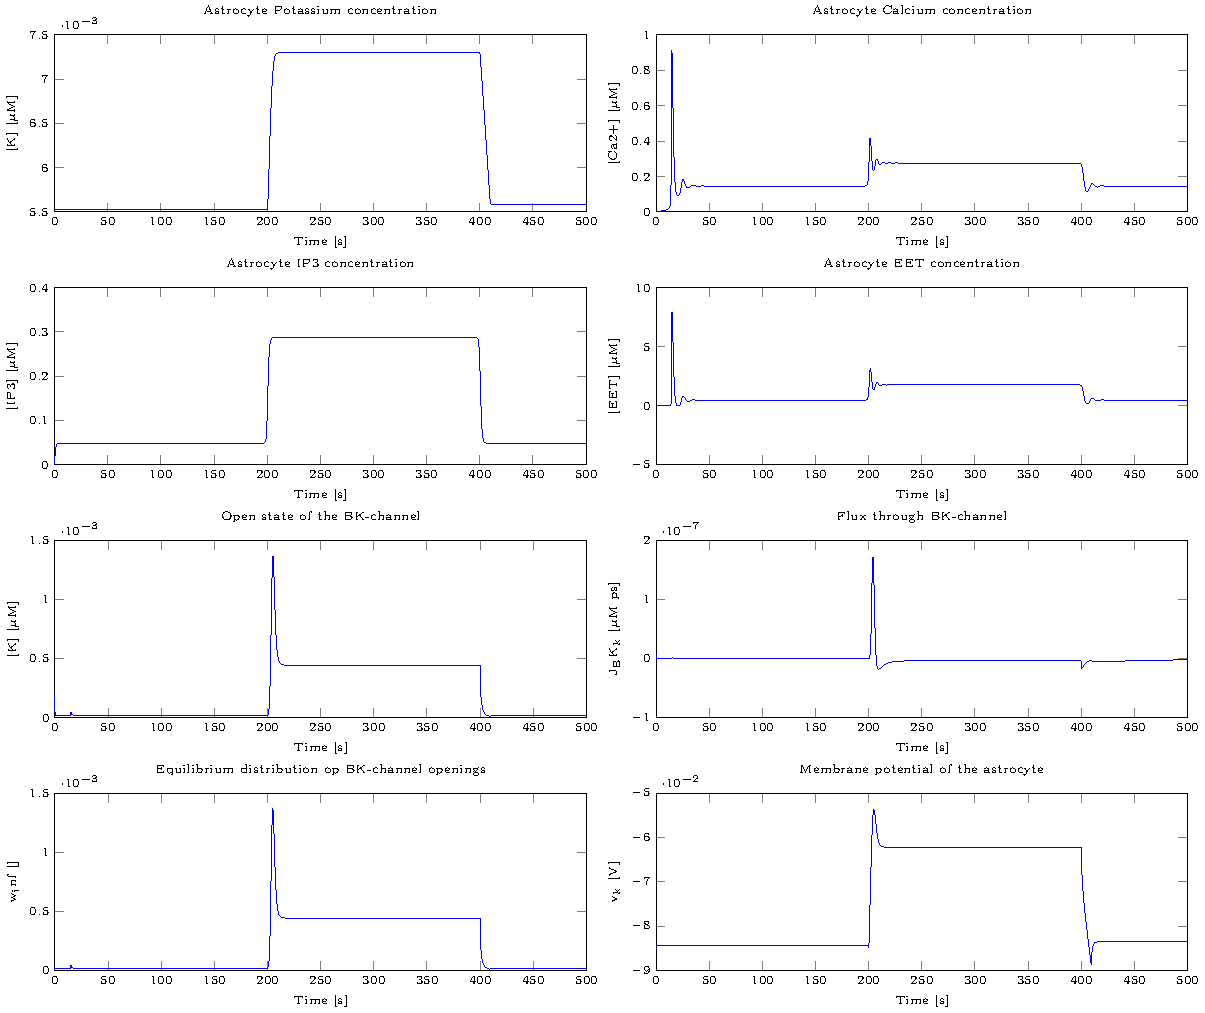
\includegraphics{figures/7_Astrocyte_equations.pdf}
			\caption{The solutions of astrocytic equations and the BK-channel}
			\label{fig:7ACe}
		\end{figure}
		
		\begin{figure}[h!]
			\centering
			\tiny 
			\setlength\figureheight{3 cm} 
			\setlength\figurewidth{4.5 cm}
			%% % This file was created by matlab2tikz v0.3.3.
% Copyright (c) 2008--2013, Nico Schlömer <nico.schloemer@gmail.com>
% All rights reserved.
% 
% The latest updates can be retrieved from
%   http://www.mathworks.com/matlabcentral/fileexchange/22022-matlab2tikz
% where you can also make suggestions and rate matlab2tikz.
% 
% 
% 
\begin{tikzpicture}

\begin{axis}[%
width=\figurewidth,
height=\figureheight,
scale only axis,
xmin=0,
xmax=500,
xlabel={time in s},
ymin=0,
ymax=0.2,
ylabel={$\text{J}_\text{ }\text{SRuptake}_\text{i}$},
name=plot5,
title={$\text{J}_\text{ }\text{SRuptake}_\text{i}$}
]
\addplot [
color=blue,
solid,
forget plot
]
table[row sep=crcr]{
0 0.02005\\
0.0011996 0.020021\\
0.0023992 0.019992\\
0.0035988 0.019963\\
0.0085566 0.019846\\
0.013514 0.01973\\
0.018472 0.019615\\
0.02343 0.019502\\
0.033542 0.019278\\
0.043655 0.01906\\
0.053767 0.018849\\
0.063879 0.018645\\
0.073991 0.018449\\
0.084819 0.018247\\
0.095647 0.018053\\
0.10647 0.017867\\
0.1173 0.017689\\
0.12813 0.01752\\
0.14659 0.017252\\
0.16505 0.017009\\
0.18351 0.016793\\
0.20197 0.016605\\
0.22042 0.016448\\
0.26398 0.016225\\
0.30753 0.016282\\
0.35108 0.016763\\
0.37397 0.017235\\
0.38969 0.017649\\
0.4054 0.018118\\
0.42111 0.018626\\
0.43393 0.019058\\
0.44676 0.019499\\
0.45959 0.019946\\
0.47242 0.020398\\
0.48525 0.020851\\
0.50035 0.021387\\
0.51544 0.021924\\
0.53054 0.022462\\
0.54564 0.022999\\
0.56073 0.023535\\
0.57728 0.024122\\
0.59382 0.024707\\
0.61036 0.025291\\
0.6269 0.025873\\
0.64344 0.026453\\
0.65998 0.02703\\
0.69992 0.028413\\
0.73986 0.029778\\
0.77979 0.031122\\
0.81973 0.032442\\
0.85967 0.033737\\
0.99616 0.037951\\
1.1327 0.041795\\
1.2692 0.045243\\
1.4056 0.048295\\
1.6062 0.052095\\
1.8067 0.055167\\
2.0072 0.05763\\
2.2078 0.059601\\
2.4083 0.061184\\
2.8551 0.063692\\
3.302 0.065379\\
3.7488 0.066663\\
4.1956 0.067742\\
4.6425 0.068716\\
5.3586 0.070197\\
6.0748 0.071705\\
6.791 0.073284\\
7.5072 0.074934\\
8.2234 0.076642\\
9.2234 0.079111\\
10.223 0.081686\\
11.223 0.084405\\
12.223 0.087242\\
12.523 0.088101\\
12.823 0.088954\\
13.123 0.089808\\
13.423 0.090669\\
13.513 0.090929\\
13.603 0.091189\\
13.693 0.091449\\
13.783 0.091709\\
13.873 0.091969\\
13.929 0.09213\\
13.948 0.092185\\
13.967 0.092239\\
13.986 0.092294\\
14.004 0.092349\\
14.023 0.092404\\
14.079 0.092563\\
14.134 0.092723\\
14.189 0.092883\\
14.244 0.093043\\
14.299 0.093202\\
14.354 0.093362\\
14.409 0.093522\\
14.465 0.093681\\
14.52 0.093842\\
14.575 0.094002\\
14.631 0.094163\\
14.686 0.094323\\
14.742 0.094484\\
14.811 0.094684\\
14.88 0.094885\\
14.95 0.095086\\
15.019 0.095286\\
15.089 0.095486\\
15.202 0.095811\\
15.315 0.096136\\
15.428 0.09646\\
15.541 0.096784\\
15.654 0.097107\\
15.804 0.097535\\
15.954 0.097963\\
16.104 0.098388\\
16.255 0.098813\\
16.405 0.099235\\
16.675 0.099991\\
16.946 0.10074\\
17.216 0.10148\\
17.487 0.10222\\
17.757 0.10294\\
18.061 0.10375\\
18.364 0.10454\\
18.667 0.10531\\
18.971 0.10608\\
19.274 0.10683\\
19.375 0.10708\\
19.476 0.10732\\
19.576 0.10756\\
19.677 0.10781\\
19.778 0.10805\\
19.938 0.10842\\
20.097 0.1088\\
20.257 0.10917\\
20.416 0.10953\\
20.576 0.10989\\
20.994 0.11082\\
21.411 0.11172\\
21.828 0.1126\\
22.056 0.11306\\
22.119 0.11319\\
22.183 0.11332\\
22.247 0.11345\\
22.31 0.11358\\
22.432 0.11382\\
22.554 0.11406\\
22.676 0.1143\\
22.798 0.11454\\
22.92 0.11477\\
23.367 0.11562\\
23.684 0.11621\\
24 0.11679\\
24.242 0.11722\\
24.484 0.11765\\
24.726 0.11807\\
24.968 0.11849\\
25.298 0.11905\\
25.628 0.11961\\
25.958 0.12015\\
26.288 0.12069\\
26.618 0.12122\\
27.087 0.12196\\
27.556 0.12268\\
28.025 0.1234\\
28.494 0.1241\\
28.964 0.12479\\
29.615 0.12572\\
30.266 0.12664\\
30.917 0.12753\\
31.569 0.12841\\
32.372 0.12946\\
33.175 0.13049\\
33.979 0.13148\\
34.782 0.13246\\
35.586 0.13341\\
36.23 0.13416\\
36.875 0.1349\\
37.52 0.13562\\
38.164 0.13634\\
38.969 0.1372\\
39.774 0.13803\\
40.579 0.1388\\
41.384 0.13949\\
42.189 0.14009\\
43.189 0.14064\\
44.189 0.14093\\
45.189 0.14096\\
46.189 0.14071\\
47.189 0.14024\\
48.189 0.13963\\
49.189 0.13896\\
50.189 0.13831\\
51.189 0.13776\\
52.189 0.13732\\
53.189 0.137\\
54.189 0.13681\\
55.189 0.13672\\
56.189 0.1367\\
57.189 0.13675\\
58.189 0.13684\\
59.189 0.13695\\
60.189 0.13709\\
61.189 0.13723\\
62.189 0.13738\\
63.189 0.13753\\
64.189 0.13766\\
65.189 0.13779\\
66.189 0.13789\\
67.189 0.13798\\
68.189 0.13804\\
69.189 0.13809\\
70.189 0.13811\\
71.189 0.13811\\
72.189 0.13809\\
73.189 0.13806\\
74.189 0.13802\\
75.189 0.13798\\
76.189 0.13793\\
77.189 0.13788\\
78.189 0.13784\\
79.189 0.1378\\
80.189 0.13777\\
81.189 0.13773\\
82.189 0.13771\\
83.189 0.13769\\
84.189 0.13768\\
85.189 0.13767\\
86.189 0.13766\\
87.189 0.13766\\
88.189 0.13766\\
89.189 0.13766\\
90.189 0.13767\\
91.189 0.13767\\
92.189 0.13768\\
93.189 0.13768\\
94.189 0.13769\\
95.189 0.13769\\
96.189 0.13769\\
97.189 0.13769\\
98.189 0.13769\\
99.189 0.13768\\
100.19 0.13768\\
101.19 0.13767\\
102.19 0.13767\\
103.19 0.13766\\
104.19 0.13765\\
105.19 0.13764\\
106.19 0.13764\\
107.19 0.13763\\
108.19 0.13762\\
109.19 0.13762\\
110.19 0.13761\\
111.19 0.13761\\
112.19 0.1376\\
113.19 0.1376\\
114.19 0.13759\\
115.19 0.13759\\
116.19 0.13759\\
117.19 0.13758\\
118.19 0.13758\\
119.19 0.13758\\
120.19 0.13757\\
121.19 0.13757\\
122.19 0.13757\\
123.19 0.13757\\
124.19 0.13756\\
125.19 0.13756\\
126.19 0.13756\\
127.19 0.13756\\
128.19 0.13755\\
129.19 0.13755\\
130.19 0.13755\\
131.19 0.13754\\
132.19 0.13754\\
133.19 0.13754\\
134.19 0.13754\\
135.19 0.13753\\
136.19 0.13753\\
137.19 0.13753\\
138.19 0.13753\\
139.19 0.13752\\
140.19 0.13752\\
141.19 0.13752\\
142.19 0.13752\\
143.19 0.13751\\
144.19 0.13751\\
145.19 0.13751\\
146.19 0.13751\\
147.19 0.13751\\
148.19 0.13751\\
149.19 0.1375\\
150.19 0.1375\\
151.19 0.1375\\
152.19 0.1375\\
153.19 0.1375\\
154.19 0.13749\\
155.19 0.13749\\
156.19 0.13749\\
157.19 0.13749\\
158.19 0.13749\\
159.19 0.13749\\
160.19 0.13748\\
161.19 0.13748\\
162.19 0.13748\\
163.19 0.13748\\
164.19 0.13748\\
165.19 0.13748\\
166.19 0.13748\\
167.19 0.13748\\
168.19 0.13747\\
169.19 0.13747\\
170.19 0.13747\\
171.19 0.13747\\
172.19 0.13747\\
173.19 0.13747\\
174.19 0.13747\\
175.19 0.13747\\
176.19 0.13747\\
177.19 0.13746\\
178.19 0.13746\\
179.19 0.13746\\
180.19 0.13746\\
181.19 0.13746\\
182.19 0.13746\\
183.19 0.13746\\
184.19 0.13746\\
185.19 0.13746\\
186.19 0.13746\\
187.19 0.13746\\
188.19 0.13745\\
189.19 0.13745\\
190.19 0.13745\\
191.19 0.13745\\
192.19 0.13745\\
193.19 0.13745\\
194.19 0.13745\\
195.19 0.13745\\
196.19 0.13745\\
196.81 0.13745\\
197.25 0.13745\\
197.57 0.13745\\
197.82 0.13745\\
198.03 0.13745\\
198.24 0.13745\\
198.38 0.13745\\
198.52 0.13745\\
198.63 0.13745\\
198.74 0.13745\\
198.83 0.13745\\
198.92 0.13745\\
199.01 0.13745\\
199.17 0.13745\\
199.32 0.13745\\
199.47 0.13745\\
199.62 0.13745\\
199.84 0.13745\\
200.07 0.13745\\
200.29 0.13745\\
200.51 0.13745\\
200.69 0.13745\\
200.87 0.13744\\
201.05 0.13744\\
201.23 0.13743\\
201.42 0.13742\\
201.6 0.13739\\
201.79 0.13734\\
201.97 0.13728\\
202.15 0.13717\\
202.34 0.13702\\
202.63 0.13662\\
202.92 0.13592\\
203.21 0.13476\\
203.5 0.1329\\
203.79 0.13005\\
204.09 0.12568\\
204.39 0.11953\\
204.69 0.11154\\
204.94 0.10382\\
205.19 0.09564\\
205.44 0.087671\\
205.68 0.080501\\
205.85 0.07616\\
206.02 0.072296\\
206.19 0.068874\\
206.36 0.065853\\
206.6 0.062156\\
206.84 0.059072\\
207.08 0.056499\\
207.32 0.054347\\
207.65 0.051933\\
207.99 0.050025\\
208.32 0.048504\\
208.65 0.047281\\
208.99 0.046291\\
209.66 0.044808\\
210.18 0.043996\\
210.7 0.043382\\
211.22 0.042915\\
211.74 0.042559\\
212.26 0.042286\\
212.9 0.042037\\
213.54 0.041862\\
214.18 0.041745\\
214.82 0.041676\\
215.46 0.041644\\
216.16 0.041644\\
216.87 0.041674\\
217.57 0.041727\\
218.27 0.041798\\
218.98 0.041884\\
219.98 0.042025\\
220.98 0.042181\\
221.98 0.042347\\
222.98 0.042518\\
223.98 0.042687\\
224.98 0.04285\\
225.98 0.043002\\
226.98 0.043144\\
227.98 0.043275\\
228.98 0.043398\\
229.98 0.04351\\
230.98 0.04361\\
231.98 0.043696\\
232.98 0.043772\\
233.98 0.043837\\
234.98 0.043893\\
235.98 0.043943\\
236.98 0.043987\\
237.98 0.044026\\
238.98 0.044061\\
239.98 0.044093\\
240.98 0.044123\\
241.98 0.044154\\
242.98 0.044186\\
243.98 0.044218\\
244.98 0.044251\\
245.98 0.044285\\
246.98 0.044321\\
247.98 0.044357\\
248.98 0.044394\\
249.98 0.044431\\
250.98 0.044469\\
251.98 0.044507\\
252.98 0.044545\\
253.98 0.044583\\
254.98 0.04462\\
255.98 0.044656\\
256.98 0.044692\\
257.98 0.044727\\
258.98 0.04476\\
259.98 0.044793\\
260.98 0.044824\\
261.98 0.044855\\
262.98 0.044884\\
263.98 0.044912\\
264.98 0.04494\\
265.98 0.044966\\
266.98 0.044991\\
267.98 0.045016\\
268.98 0.04504\\
269.98 0.045064\\
270.98 0.045086\\
271.98 0.045109\\
272.98 0.04513\\
273.98 0.045152\\
274.98 0.045173\\
275.98 0.045193\\
276.98 0.045213\\
277.98 0.045233\\
278.98 0.045253\\
279.98 0.045272\\
280.98 0.045291\\
281.98 0.04531\\
282.98 0.045328\\
283.98 0.045346\\
284.98 0.045364\\
285.98 0.045381\\
286.98 0.045398\\
287.98 0.045414\\
288.98 0.04543\\
289.98 0.045446\\
290.98 0.045461\\
291.98 0.045476\\
292.98 0.045491\\
293.98 0.045505\\
294.98 0.045519\\
295.98 0.045533\\
296.98 0.045546\\
297.98 0.045559\\
298.98 0.045572\\
299.98 0.045585\\
300.98 0.045597\\
301.98 0.045608\\
302.98 0.04562\\
303.98 0.045631\\
304.98 0.045642\\
305.98 0.045653\\
306.98 0.045664\\
307.98 0.045674\\
308.98 0.045684\\
309.98 0.045694\\
310.98 0.045704\\
311.98 0.045713\\
312.98 0.045722\\
313.98 0.045731\\
314.98 0.04574\\
315.98 0.045749\\
316.98 0.045757\\
317.98 0.045766\\
318.98 0.045774\\
319.98 0.045781\\
320.98 0.045789\\
321.98 0.045797\\
322.98 0.045804\\
323.98 0.045811\\
324.98 0.045818\\
325.98 0.045825\\
326.98 0.045832\\
327.98 0.045838\\
328.98 0.045845\\
329.98 0.045851\\
330.98 0.045857\\
331.98 0.045863\\
332.98 0.045869\\
333.98 0.045875\\
334.98 0.04588\\
335.98 0.045885\\
336.98 0.045891\\
337.98 0.045896\\
338.98 0.045901\\
339.98 0.045906\\
340.98 0.045911\\
341.98 0.045915\\
342.98 0.04592\\
343.98 0.045925\\
344.98 0.045929\\
345.98 0.045933\\
346.98 0.045937\\
347.98 0.045942\\
348.98 0.045946\\
349.98 0.04595\\
350.98 0.045953\\
351.98 0.045957\\
352.98 0.045961\\
353.98 0.045964\\
354.98 0.045968\\
355.98 0.045971\\
356.98 0.045974\\
357.98 0.045978\\
358.98 0.045981\\
359.98 0.045984\\
360.98 0.045987\\
361.98 0.04599\\
362.98 0.045993\\
363.98 0.045996\\
364.98 0.045998\\
365.98 0.046001\\
366.98 0.046004\\
367.98 0.046006\\
368.98 0.046009\\
369.98 0.046011\\
370.98 0.046014\\
371.98 0.046016\\
372.98 0.046018\\
373.98 0.04602\\
374.98 0.046023\\
375.98 0.046025\\
376.98 0.046027\\
377.98 0.046029\\
378.98 0.046031\\
379.98 0.046033\\
380.98 0.046035\\
381.98 0.046036\\
382.98 0.046038\\
383.98 0.04604\\
384.98 0.046042\\
385.98 0.046043\\
386.98 0.046045\\
387.98 0.046047\\
388.98 0.046048\\
389.98 0.04605\\
390.98 0.046051\\
391.98 0.046053\\
392.98 0.046054\\
393.98 0.046055\\
394.98 0.046057\\
395.98 0.046058\\
396.98 0.046059\\
397.98 0.046061\\
398.44 0.046061\\
398.8 0.046062\\
399.07 0.046062\\
399.35 0.046062\\
399.55 0.046062\\
399.76 0.046062\\
399.96 0.046063\\
400.26 0.046067\\
400.34 0.04607\\
400.43 0.046075\\
400.52 0.046082\\
400.61 0.046091\\
400.92 0.046147\\
401.24 0.046238\\
401.56 0.046364\\
401.87 0.046522\\
402.11 0.046662\\
402.35 0.046817\\
402.59 0.046986\\
402.83 0.047165\\
403.14 0.047413\\
403.45 0.047675\\
403.77 0.047946\\
404.08 0.048225\\
404.39 0.048508\\
404.93 0.049009\\
405.47 0.049508\\
406.02 0.05\\
406.56 0.050478\\
407.1 0.050941\\
408.1 0.051733\\
408.77 0.052203\\
409.43 0.052618\\
410.1 0.052982\\
410.61 0.053249\\
411.12 0.053535\\
411.63 0.053867\\
412.15 0.054264\\
412.66 0.054731\\
413.31 0.055426\\
413.95 0.056242\\
414.6 0.057188\\
415.25 0.058279\\
415.9 0.059534\\
416.77 0.061546\\
417.65 0.063987\\
418.52 0.066917\\
419.4 0.070294\\
420.28 0.07382\\
421.2 0.077115\\
422.12 0.079487\\
423.04 0.080965\\
423.96 0.082114\\
424.89 0.083584\\
425.81 0.085562\\
426.73 0.087712\\
427.68 0.089691\\
428.64 0.091314\\
429.59 0.092769\\
430.55 0.094279\\
431.5 0.0959\\
432.5 0.097598\\
433.5 0.09916\\
434.5 0.10056\\
435.5 0.10189\\
436.5 0.10321\\
437.5 0.10452\\
438.5 0.10576\\
439.5 0.10689\\
440.5 0.10793\\
441.5 0.10891\\
442.5 0.10984\\
443.5 0.1107\\
444.5 0.1115\\
445.5 0.11226\\
446.5 0.11299\\
447.5 0.11367\\
448.5 0.11433\\
449.5 0.11496\\
450.5 0.11556\\
451.5 0.11613\\
452.5 0.11667\\
453.5 0.1172\\
454.5 0.11771\\
455.5 0.1182\\
456.5 0.11867\\
457.5 0.11913\\
458.5 0.11958\\
459.5 0.12002\\
460.5 0.12045\\
461.5 0.12086\\
462.5 0.12126\\
463.5 0.12166\\
464.5 0.12204\\
465.5 0.12241\\
466.5 0.12277\\
467.5 0.12313\\
468.5 0.12347\\
469.5 0.12381\\
470.5 0.12413\\
471.5 0.12445\\
472.5 0.12476\\
473.5 0.12506\\
474.5 0.12536\\
475.5 0.12564\\
476.5 0.12592\\
477.5 0.1262\\
478.5 0.12646\\
479.5 0.12672\\
480.5 0.12697\\
481.5 0.12721\\
482.5 0.12745\\
483.5 0.12768\\
484.5 0.12791\\
485.5 0.12813\\
486.5 0.12834\\
487.5 0.12855\\
488.5 0.12876\\
489.5 0.12896\\
490.5 0.12915\\
491.5 0.12934\\
492.5 0.12952\\
493.5 0.1297\\
494.5 0.12987\\
495.5 0.13004\\
496.5 0.13021\\
497.5 0.13037\\
498.5 0.13053\\
499.5 0.13068\\
500 0.13076\\
};
\end{axis}

\begin{axis}[%
width=\figurewidth,
height=\figureheight,
scale only axis,
xmin=0,
xmax=500,
xlabel={time in s},
ymin=-0.01,
ymax=0.03,
ylabel={$\text{Ca}_\text{ }\text{coup}_\text{i}$},
name=plot2,
at=(plot5.above north west),
anchor=below south west,
title={$\text{Ca}_\text{ }\text{coup}_\text{i}$}
]
\addplot [
color=blue,
solid,
forget plot
]
table[row sep=crcr]{
0 -0\\
0.0011996 2.2127e-07\\
0.0023992 5.5314e-07\\
0.0035988 9.9233e-07\\
0.0085566 3.7299e-06\\
0.013514 7.8673e-06\\
0.018472 1.3155e-05\\
0.02343 1.9356e-05\\
0.033542 3.4093e-05\\
0.043655 5.054e-05\\
0.053767 6.7812e-05\\
0.063879 8.537e-05\\
0.073991 0.00010287\\
0.084819 0.00012129\\
0.095647 0.00013918\\
0.10647 0.00015638\\
0.1173 0.00017282\\
0.12813 0.00018841\\
0.14659 0.00021289\\
0.16505 0.00023447\\
0.18351 0.0002529\\
0.20197 0.00026787\\
0.22042 0.00027899\\
0.26398 0.00028604\\
0.30753 0.00025576\\
0.35108 0.00016851\\
0.37397 9.3924e-05\\
0.38969 3.1601e-05\\
0.4054 -3.7242e-05\\
0.42111 -0.00011002\\
0.43393 -0.00017085\\
0.44676 -0.00023209\\
0.45959 -0.00029329\\
0.47242 -0.00035418\\
0.48525 -0.0004146\\
0.50035 -0.00048497\\
0.51544 -0.00055445\\
0.53054 -0.00062298\\
0.54564 -0.00069052\\
0.56073 -0.00075706\\
0.57728 -0.00082881\\
0.59382 -0.00089935\\
0.61036 -0.00096868\\
0.6269 -0.0010368\\
0.64344 -0.0011038\\
0.65998 -0.0011695\\
0.69992 -0.0013235\\
0.73986 -0.0014706\\
0.77979 -0.0016111\\
0.81973 -0.001745\\
0.85967 -0.0018724\\
0.99616 -0.0022614\\
1.1327 -0.0025817\\
1.2692 -0.002839\\
1.4056 -0.0030393\\
1.6062 -0.0032423\\
1.8067 -0.003353\\
2.0072 -0.0033884\\
2.2078 -0.003363\\
2.4083 -0.0032886\\
2.8551 -0.0029914\\
3.302 -0.002579\\
3.7488 -0.0021043\\
4.1956 -0.0015996\\
4.6425 -0.0010859\\
5.3586 -0.0002766\\
6.0748 0.00048183\\
6.791 0.0011728\\
7.5072 0.0017928\\
8.2234 0.0023442\\
9.2234 0.0030094\\
10.223 0.0035654\\
11.223 0.0040271\\
12.223 0.0044129\\
12.523 0.0045171\\
12.823 0.0046171\\
13.123 0.0047128\\
13.423 0.0048041\\
13.513 0.0048307\\
13.603 0.004857\\
13.693 0.0048829\\
13.783 0.0049085\\
13.873 0.0049339\\
13.929 0.0049493\\
13.948 0.0049546\\
13.967 0.0049598\\
13.986 0.004965\\
14.004 0.0049703\\
14.023 0.0049755\\
14.079 0.0049905\\
14.134 0.0050055\\
14.189 0.0050204\\
14.244 0.0050352\\
14.299 0.0050498\\
14.354 0.0050644\\
14.409 0.0050789\\
14.465 0.0050933\\
14.52 0.0051077\\
14.575 0.005122\\
14.631 0.0051362\\
14.686 0.0051503\\
14.742 0.0051643\\
14.811 0.0051818\\
14.88 0.0051992\\
14.95 0.0052164\\
15.019 0.0052335\\
15.089 0.0052505\\
15.202 0.005278\\
15.315 0.0053051\\
15.428 0.005332\\
15.541 0.0053587\\
15.654 0.0053851\\
15.804 0.00542\\
15.954 0.0054544\\
16.104 0.0054886\\
16.255 0.0055224\\
16.405 0.0055559\\
16.675 0.0056157\\
16.946 0.0056749\\
17.216 0.0057336\\
17.487 0.0057919\\
17.757 0.0058501\\
18.061 0.0059153\\
18.364 0.0059805\\
18.667 0.006046\\
18.971 0.0061118\\
19.274 0.0061782\\
19.375 0.0062004\\
19.476 0.0062227\\
19.576 0.006245\\
19.677 0.0062675\\
19.778 0.00629\\
19.938 0.0063258\\
20.097 0.006362\\
20.257 0.0063983\\
20.416 0.006435\\
20.576 0.0064719\\
20.994 0.0065699\\
21.411 0.0066702\\
21.828 0.0067728\\
22.056 0.0068297\\
22.119 0.0068458\\
22.183 0.0068619\\
22.247 0.0068782\\
22.31 0.0068944\\
22.432 0.0069257\\
22.554 0.0069573\\
22.676 0.0069891\\
22.798 0.0070211\\
22.92 0.0070534\\
23.367 0.007174\\
23.684 0.0072615\\
24 0.0073508\\
24.242 0.0074203\\
24.484 0.0074909\\
24.726 0.0075627\\
24.968 0.0076356\\
25.298 0.007737\\
25.628 0.0078407\\
25.958 0.0079467\\
26.288 0.0080552\\
26.618 0.0081663\\
27.087 0.0083287\\
27.556 0.0084967\\
28.025 0.0086705\\
28.494 0.0088503\\
28.964 0.0090365\\
29.615 0.0093061\\
30.266 0.0095893\\
30.917 0.0098867\\
31.569 0.010199\\
32.372 0.010606\\
33.175 0.011037\\
33.979 0.011494\\
34.782 0.011975\\
35.586 0.01248\\
36.23 0.012899\\
36.875 0.013328\\
37.52 0.013764\\
38.164 0.014203\\
38.969 0.014745\\
39.774 0.01527\\
40.579 0.015761\\
41.384 0.016204\\
42.189 0.016583\\
43.189 0.016948\\
44.189 0.017188\\
45.189 0.017301\\
46.189 0.017301\\
47.189 0.017207\\
48.189 0.017043\\
49.189 0.016832\\
50.189 0.016599\\
51.189 0.01636\\
52.189 0.016128\\
53.189 0.015916\\
54.189 0.015731\\
55.189 0.015578\\
56.189 0.01546\\
57.189 0.015377\\
58.189 0.015327\\
59.189 0.015308\\
60.189 0.015315\\
61.189 0.015343\\
62.189 0.015388\\
63.189 0.015444\\
64.189 0.015509\\
65.189 0.015576\\
66.189 0.015643\\
67.189 0.015707\\
68.189 0.015764\\
69.189 0.01581\\
70.189 0.015846\\
71.189 0.015872\\
72.189 0.015891\\
73.189 0.015901\\
74.189 0.015904\\
75.189 0.0159\\
76.189 0.015889\\
77.189 0.015875\\
78.189 0.015859\\
79.189 0.015843\\
80.189 0.015826\\
81.189 0.01581\\
82.189 0.015796\\
83.189 0.015784\\
84.189 0.015774\\
85.189 0.015766\\
86.189 0.015761\\
87.189 0.015758\\
88.189 0.015757\\
89.189 0.015758\\
90.189 0.01576\\
91.189 0.015764\\
92.189 0.015768\\
93.189 0.015773\\
94.189 0.015777\\
95.189 0.015782\\
96.189 0.015786\\
97.189 0.01579\\
98.189 0.015793\\
99.189 0.015795\\
100.19 0.015797\\
101.19 0.015799\\
102.19 0.015799\\
103.19 0.0158\\
104.19 0.0158\\
105.19 0.015799\\
106.19 0.015798\\
107.19 0.015798\\
108.19 0.015797\\
109.19 0.015796\\
110.19 0.015795\\
111.19 0.015794\\
112.19 0.015794\\
113.19 0.015793\\
114.19 0.015793\\
115.19 0.015793\\
116.19 0.015793\\
117.19 0.015793\\
118.19 0.015793\\
119.19 0.015794\\
120.19 0.015794\\
121.19 0.015794\\
122.19 0.015795\\
123.19 0.015795\\
124.19 0.015796\\
125.19 0.015796\\
126.19 0.015796\\
127.19 0.015796\\
128.19 0.015797\\
129.19 0.015797\\
130.19 0.015797\\
131.19 0.015797\\
132.19 0.015797\\
133.19 0.015797\\
134.19 0.015797\\
135.19 0.015798\\
136.19 0.015798\\
137.19 0.015798\\
138.19 0.015798\\
139.19 0.015798\\
140.19 0.015798\\
141.19 0.015798\\
142.19 0.015798\\
143.19 0.015798\\
144.19 0.015798\\
145.19 0.015798\\
146.19 0.015798\\
147.19 0.015798\\
148.19 0.015798\\
149.19 0.015798\\
150.19 0.015799\\
151.19 0.015799\\
152.19 0.015799\\
153.19 0.015799\\
154.19 0.015799\\
155.19 0.015799\\
156.19 0.015799\\
157.19 0.015799\\
158.19 0.015799\\
159.19 0.015799\\
160.19 0.015799\\
161.19 0.015799\\
162.19 0.015799\\
163.19 0.015799\\
164.19 0.015799\\
165.19 0.015799\\
166.19 0.0158\\
167.19 0.0158\\
168.19 0.0158\\
169.19 0.0158\\
170.19 0.0158\\
171.19 0.0158\\
172.19 0.0158\\
173.19 0.0158\\
174.19 0.0158\\
175.19 0.0158\\
176.19 0.0158\\
177.19 0.0158\\
178.19 0.0158\\
179.19 0.0158\\
180.19 0.0158\\
181.19 0.0158\\
182.19 0.0158\\
183.19 0.0158\\
184.19 0.0158\\
185.19 0.0158\\
186.19 0.0158\\
187.19 0.0158\\
188.19 0.015801\\
189.19 0.015801\\
190.19 0.015801\\
191.19 0.015801\\
192.19 0.015801\\
193.19 0.015801\\
194.19 0.015801\\
195.19 0.015801\\
196.19 0.015801\\
196.81 0.015801\\
197.25 0.015801\\
197.57 0.015801\\
197.82 0.015801\\
198.03 0.015801\\
198.24 0.015801\\
198.38 0.015801\\
198.52 0.015801\\
198.63 0.015801\\
198.74 0.015801\\
198.83 0.015801\\
198.92 0.015801\\
199.01 0.015801\\
199.17 0.015801\\
199.32 0.015801\\
199.47 0.015801\\
199.62 0.015801\\
199.84 0.015801\\
200.07 0.015801\\
200.29 0.015801\\
200.51 0.015801\\
200.69 0.015801\\
200.87 0.015801\\
201.05 0.015801\\
201.23 0.015802\\
201.42 0.015802\\
201.6 0.015804\\
201.79 0.015806\\
201.97 0.01581\\
202.15 0.015815\\
202.34 0.015823\\
202.63 0.015844\\
202.92 0.01588\\
203.21 0.015939\\
203.5 0.016035\\
203.79 0.016183\\
204.09 0.016412\\
204.39 0.016739\\
204.69 0.017171\\
204.94 0.017598\\
205.19 0.018062\\
205.44 0.018525\\
205.68 0.018948\\
205.85 0.019207\\
206.02 0.019438\\
206.19 0.019642\\
206.36 0.019821\\
206.6 0.020036\\
206.84 0.020209\\
207.08 0.020346\\
207.32 0.020453\\
207.65 0.020559\\
207.99 0.020626\\
208.32 0.020665\\
208.65 0.020681\\
208.99 0.02068\\
209.66 0.020642\\
210.18 0.020594\\
210.7 0.020538\\
211.22 0.020479\\
211.74 0.020419\\
212.26 0.020363\\
212.9 0.020299\\
213.54 0.020245\\
214.18 0.0202\\
214.82 0.020166\\
215.46 0.020141\\
216.16 0.020127\\
216.87 0.020123\\
217.57 0.02013\\
218.27 0.020146\\
218.98 0.02017\\
219.98 0.020215\\
220.98 0.02027\\
221.98 0.020331\\
222.98 0.020395\\
223.98 0.020458\\
224.98 0.020517\\
225.98 0.02057\\
226.98 0.020615\\
227.98 0.020651\\
228.98 0.020678\\
229.98 0.020694\\
230.98 0.020701\\
231.98 0.0207\\
232.98 0.02069\\
233.98 0.020675\\
234.98 0.020655\\
235.98 0.020632\\
236.98 0.020606\\
237.98 0.020581\\
238.98 0.020556\\
239.98 0.020533\\
240.98 0.020513\\
241.98 0.020495\\
242.98 0.020481\\
243.98 0.020469\\
244.98 0.02046\\
245.98 0.020453\\
246.98 0.020449\\
247.98 0.020447\\
248.98 0.020447\\
249.98 0.020448\\
250.98 0.02045\\
251.98 0.020452\\
252.98 0.020455\\
253.98 0.020458\\
254.98 0.02046\\
255.98 0.020463\\
256.98 0.020464\\
257.98 0.020466\\
258.98 0.020466\\
259.98 0.020466\\
260.98 0.020466\\
261.98 0.020465\\
262.98 0.020463\\
263.98 0.020461\\
264.98 0.020459\\
265.98 0.020456\\
266.98 0.020453\\
267.98 0.02045\\
268.98 0.020447\\
269.98 0.020445\\
270.98 0.020442\\
271.98 0.020439\\
272.98 0.020437\\
273.98 0.020435\\
274.98 0.020432\\
275.98 0.02043\\
276.98 0.020429\\
277.98 0.020427\\
278.98 0.020426\\
279.98 0.020425\\
280.98 0.020423\\
281.98 0.020422\\
282.98 0.020421\\
283.98 0.02042\\
284.98 0.02042\\
285.98 0.020419\\
286.98 0.020418\\
287.98 0.020417\\
288.98 0.020416\\
289.98 0.020415\\
290.98 0.020414\\
291.98 0.020413\\
292.98 0.020413\\
293.98 0.020412\\
294.98 0.020411\\
295.98 0.02041\\
296.98 0.020409\\
297.98 0.020408\\
298.98 0.020407\\
299.98 0.020406\\
300.98 0.020405\\
301.98 0.020404\\
302.98 0.020404\\
303.98 0.020403\\
304.98 0.020402\\
305.98 0.020401\\
306.98 0.0204\\
307.98 0.0204\\
308.98 0.020399\\
309.98 0.020398\\
310.98 0.020398\\
311.98 0.020397\\
312.98 0.020396\\
313.98 0.020396\\
314.98 0.020395\\
315.98 0.020395\\
316.98 0.020394\\
317.98 0.020394\\
318.98 0.020393\\
319.98 0.020393\\
320.98 0.020392\\
321.98 0.020392\\
322.98 0.020391\\
323.98 0.020391\\
324.98 0.02039\\
325.98 0.02039\\
326.98 0.020389\\
327.98 0.020389\\
328.98 0.020388\\
329.98 0.020388\\
330.98 0.020387\\
331.98 0.020387\\
332.98 0.020387\\
333.98 0.020386\\
334.98 0.020386\\
335.98 0.020386\\
336.98 0.020385\\
337.98 0.020385\\
338.98 0.020384\\
339.98 0.020384\\
340.98 0.020384\\
341.98 0.020384\\
342.98 0.020383\\
343.98 0.020383\\
344.98 0.020383\\
345.98 0.020382\\
346.98 0.020382\\
347.98 0.020382\\
348.98 0.020381\\
349.98 0.020381\\
350.98 0.020381\\
351.98 0.020381\\
352.98 0.02038\\
353.98 0.02038\\
354.98 0.02038\\
355.98 0.02038\\
356.98 0.02038\\
357.98 0.020379\\
358.98 0.020379\\
359.98 0.020379\\
360.98 0.020379\\
361.98 0.020379\\
362.98 0.020378\\
363.98 0.020378\\
364.98 0.020378\\
365.98 0.020378\\
366.98 0.020378\\
367.98 0.020377\\
368.98 0.020377\\
369.98 0.020377\\
370.98 0.020377\\
371.98 0.020377\\
372.98 0.020377\\
373.98 0.020376\\
374.98 0.020376\\
375.98 0.020376\\
376.98 0.020376\\
377.98 0.020376\\
378.98 0.020376\\
379.98 0.020376\\
380.98 0.020376\\
381.98 0.020375\\
382.98 0.020375\\
383.98 0.020375\\
384.98 0.020375\\
385.98 0.020375\\
386.98 0.020375\\
387.98 0.020375\\
388.98 0.020375\\
389.98 0.020375\\
390.98 0.020374\\
391.98 0.020374\\
392.98 0.020374\\
393.98 0.020374\\
394.98 0.020374\\
395.98 0.020374\\
396.98 0.020374\\
397.98 0.020374\\
398.44 0.020374\\
398.8 0.020374\\
399.07 0.020374\\
399.35 0.020374\\
399.55 0.020374\\
399.76 0.020374\\
399.96 0.020374\\
400.26 0.020373\\
400.34 0.020373\\
400.43 0.020373\\
400.52 0.020372\\
400.61 0.020371\\
400.92 0.020367\\
401.24 0.020359\\
401.56 0.020349\\
401.87 0.020336\\
402.11 0.020325\\
402.35 0.020313\\
402.59 0.020299\\
402.83 0.020285\\
403.14 0.020266\\
403.45 0.020247\\
403.77 0.020227\\
404.08 0.020206\\
404.39 0.020186\\
404.93 0.020151\\
405.47 0.020117\\
406.02 0.020085\\
406.56 0.020055\\
407.1 0.020028\\
408.1 0.019984\\
408.77 0.01996\\
409.43 0.01994\\
410.1 0.019925\\
410.61 0.019914\\
411.12 0.019902\\
411.63 0.019886\\
412.15 0.019864\\
412.66 0.019837\\
413.31 0.019795\\
413.95 0.019745\\
414.6 0.019685\\
415.25 0.019616\\
415.9 0.019537\\
416.77 0.01941\\
417.65 0.019259\\
418.52 0.01908\\
419.4 0.018881\\
420.28 0.018683\\
421.2 0.018514\\
422.12 0.018413\\
423.04 0.018371\\
423.96 0.018347\\
424.89 0.018297\\
425.81 0.01821\\
426.73 0.018111\\
427.68 0.018021\\
428.64 0.01795\\
429.59 0.017886\\
430.55 0.017813\\
431.5 0.017731\\
432.5 0.017643\\
433.5 0.01756\\
434.5 0.017486\\
435.5 0.017415\\
436.5 0.017344\\
437.5 0.017273\\
438.5 0.017207\\
439.5 0.017148\\
440.5 0.017095\\
441.5 0.017045\\
442.5 0.016999\\
443.5 0.016958\\
444.5 0.01692\\
445.5 0.016886\\
446.5 0.016853\\
447.5 0.016823\\
448.5 0.016794\\
449.5 0.016767\\
450.5 0.016741\\
451.5 0.016717\\
452.5 0.016693\\
453.5 0.016671\\
454.5 0.016649\\
455.5 0.016627\\
456.5 0.016607\\
457.5 0.016586\\
458.5 0.016566\\
459.5 0.016547\\
460.5 0.016527\\
461.5 0.016509\\
462.5 0.016491\\
463.5 0.016473\\
464.5 0.016456\\
465.5 0.016439\\
466.5 0.016423\\
467.5 0.016407\\
468.5 0.016392\\
469.5 0.016377\\
470.5 0.016363\\
471.5 0.016349\\
472.5 0.016336\\
473.5 0.016323\\
474.5 0.016311\\
475.5 0.016298\\
476.5 0.016287\\
477.5 0.016275\\
478.5 0.016264\\
479.5 0.016253\\
480.5 0.016242\\
481.5 0.016232\\
482.5 0.016222\\
483.5 0.016212\\
484.5 0.016202\\
485.5 0.016193\\
486.5 0.016184\\
487.5 0.016175\\
488.5 0.016166\\
489.5 0.016158\\
490.5 0.016149\\
491.5 0.016141\\
492.5 0.016133\\
493.5 0.016126\\
494.5 0.016118\\
495.5 0.016111\\
496.5 0.016104\\
497.5 0.016097\\
498.5 0.01609\\
499.5 0.016084\\
500 0.016081\\
};
\end{axis}

\begin{axis}[%
width=\figurewidth,
height=\figureheight,
scale only axis,
xmin=0,
xmax=500,
xlabel={time in s},
ymin=-20,
ymax=10,
ylabel={$\text{v}_\text{ }\text{coup}_\text{i}$},
name=plot1,
at=(plot2.left of south west),
anchor=right of south east,
title={$\text{v}_\text{ }\text{coup}_\text{i}$}
]
\addplot [
color=blue,
solid,
forget plot
]
table[row sep=crcr]{
0 -7.5\\
0.0011996 -6.6186\\
0.0023992 -5.7814\\
0.0035988 -4.9872\\
0.0085566 -2.0792\\
0.013514 0.25504\\
0.018472 2.1071\\
0.02343 3.5639\\
0.033542 5.5839\\
0.043655 6.7283\\
0.053767 7.3205\\
0.063879 7.5555\\
0.073991 7.5541\\
0.084819 7.3814\\
0.095647 7.0987\\
0.10647 6.7501\\
0.1173 6.3622\\
0.12813 5.9512\\
0.14659 5.2196\\
0.16505 4.4721\\
0.18351 3.7141\\
0.20197 2.9394\\
0.22042 2.1373\\
0.26398 0.035871\\
0.30753 -2.6206\\
0.35108 -6.2337\\
0.37397 -8.5479\\
0.38969 -10.189\\
0.4054 -11.723\\
0.42111 -13.028\\
0.43393 -13.867\\
0.44676 -14.494\\
0.45959 -14.925\\
0.47242 -15.191\\
0.48525 -15.328\\
0.50035 -15.372\\
0.51544 -15.334\\
0.53054 -15.249\\
0.54564 -15.143\\
0.56073 -15.027\\
0.57728 -14.901\\
0.59382 -14.78\\
0.61036 -14.663\\
0.6269 -14.553\\
0.64344 -14.447\\
0.65998 -14.346\\
0.69992 -14.117\\
0.73986 -13.902\\
0.77979 -13.698\\
0.81973 -13.504\\
0.85967 -13.321\\
0.99616 -12.766\\
1.1327 -12.309\\
1.2692 -11.935\\
1.4056 -11.634\\
1.6062 -11.304\\
1.8067 -11.086\\
2.0072 -10.961\\
2.2078 -10.914\\
2.4083 -10.929\\
2.8551 -11.132\\
3.302 -11.493\\
3.7488 -11.95\\
4.1956 -12.459\\
4.6425 -12.984\\
5.3586 -13.801\\
6.0748 -14.538\\
6.791 -15.173\\
7.5072 -15.703\\
8.2234 -16.128\\
9.2234 -16.569\\
10.223 -16.869\\
11.223 -17.06\\
12.223 -17.148\\
12.523 -17.153\\
12.823 -17.155\\
13.123 -17.154\\
13.423 -17.148\\
13.513 -17.145\\
13.603 -17.141\\
13.693 -17.137\\
13.783 -17.132\\
13.873 -17.127\\
13.929 -17.124\\
13.948 -17.123\\
13.967 -17.122\\
13.986 -17.121\\
14.004 -17.119\\
14.023 -17.118\\
14.079 -17.114\\
14.134 -17.11\\
14.189 -17.106\\
14.244 -17.102\\
14.299 -17.098\\
14.354 -17.093\\
14.409 -17.089\\
14.465 -17.084\\
14.52 -17.079\\
14.575 -17.074\\
14.631 -17.069\\
14.686 -17.063\\
14.742 -17.058\\
14.811 -17.051\\
14.88 -17.043\\
14.95 -17.036\\
15.019 -17.028\\
15.089 -17.02\\
15.202 -17.006\\
15.315 -16.992\\
15.428 -16.978\\
15.541 -16.963\\
15.654 -16.948\\
15.804 -16.927\\
15.954 -16.905\\
16.104 -16.883\\
16.255 -16.86\\
16.405 -16.836\\
16.675 -16.791\\
16.946 -16.745\\
17.216 -16.697\\
17.487 -16.647\\
17.757 -16.596\\
18.061 -16.538\\
18.364 -16.478\\
18.667 -16.417\\
18.971 -16.356\\
19.274 -16.294\\
19.375 -16.274\\
19.476 -16.253\\
19.576 -16.232\\
19.677 -16.212\\
19.778 -16.191\\
19.938 -16.158\\
20.097 -16.125\\
20.257 -16.093\\
20.416 -16.06\\
20.576 -16.028\\
20.994 -15.944\\
21.411 -15.862\\
21.828 -15.782\\
22.056 -15.74\\
22.119 -15.728\\
22.183 -15.716\\
22.247 -15.704\\
22.31 -15.693\\
22.432 -15.671\\
22.554 -15.649\\
22.676 -15.627\\
22.798 -15.606\\
22.92 -15.585\\
23.367 -15.509\\
23.684 -15.458\\
24 -15.409\\
24.242 -15.373\\
24.484 -15.338\\
24.726 -15.304\\
24.968 -15.271\\
25.298 -15.228\\
25.628 -15.188\\
25.958 -15.149\\
26.288 -15.113\\
26.618 -15.079\\
27.087 -15.035\\
27.556 -14.995\\
28.025 -14.959\\
28.494 -14.928\\
28.964 -14.901\\
29.615 -14.87\\
30.266 -14.846\\
30.917 -14.829\\
31.569 -14.818\\
32.372 -14.814\\
33.175 -14.818\\
33.979 -14.829\\
34.782 -14.846\\
35.586 -14.868\\
36.23 -14.887\\
36.875 -14.907\\
37.52 -14.928\\
38.164 -14.948\\
38.969 -14.972\\
39.774 -14.992\\
40.579 -15.008\\
41.384 -15.019\\
42.189 -15.028\\
43.189 -15.034\\
44.189 -15.037\\
45.189 -15.043\\
46.189 -15.053\\
47.189 -15.066\\
48.189 -15.081\\
49.189 -15.097\\
50.189 -15.107\\
51.189 -15.112\\
52.189 -15.112\\
53.189 -15.106\\
54.189 -15.093\\
55.189 -15.078\\
56.189 -15.061\\
57.189 -15.044\\
58.189 -15.029\\
59.189 -15.016\\
60.189 -15.006\\
61.189 -14.998\\
62.189 -14.993\\
63.189 -14.99\\
64.189 -14.988\\
65.189 -14.988\\
66.189 -14.989\\
67.189 -14.989\\
68.189 -14.992\\
69.189 -14.995\\
70.189 -14.997\\
71.189 -14.999\\
72.189 -15.001\\
73.189 -15.003\\
74.189 -15.004\\
75.189 -15.007\\
76.189 -15.007\\
77.189 -15.007\\
78.189 -15.006\\
79.189 -15.006\\
80.189 -15.005\\
81.189 -15.004\\
82.189 -15.002\\
83.189 -15.001\\
84.189 -14.999\\
85.189 -14.999\\
86.189 -14.997\\
87.189 -14.996\\
88.189 -14.995\\
89.189 -14.994\\
90.189 -14.993\\
91.189 -14.993\\
92.189 -14.992\\
93.189 -14.992\\
94.189 -14.991\\
95.189 -14.991\\
96.189 -14.99\\
97.189 -14.991\\
98.189 -14.989\\
99.189 -14.991\\
100.19 -14.989\\
101.19 -14.991\\
102.19 -14.989\\
103.19 -14.991\\
104.19 -14.99\\
105.19 -14.989\\
106.19 -14.989\\
107.19 -14.989\\
108.19 -14.989\\
109.19 -14.988\\
110.19 -14.988\\
111.19 -14.987\\
112.19 -14.988\\
113.19 -14.987\\
114.19 -14.987\\
115.19 -14.986\\
116.19 -14.987\\
117.19 -14.986\\
118.19 -14.986\\
119.19 -14.985\\
120.19 -14.986\\
121.19 -14.985\\
122.19 -14.986\\
123.19 -14.985\\
124.19 -14.985\\
125.19 -14.984\\
126.19 -14.984\\
127.19 -14.984\\
128.19 -14.984\\
129.19 -14.984\\
130.19 -14.984\\
131.19 -14.984\\
132.19 -14.983\\
133.19 -14.983\\
134.19 -14.983\\
135.19 -14.983\\
136.19 -14.983\\
137.19 -14.983\\
138.19 -14.982\\
139.19 -14.982\\
140.19 -14.982\\
141.19 -14.982\\
142.19 -14.982\\
143.19 -14.982\\
144.19 -14.981\\
145.19 -14.982\\
146.19 -14.981\\
147.19 -14.982\\
148.19 -14.981\\
149.19 -14.981\\
150.19 -14.981\\
151.19 -14.981\\
152.19 -14.98\\
153.19 -14.981\\
154.19 -14.98\\
155.19 -14.981\\
156.19 -14.98\\
157.19 -14.981\\
158.19 -14.981\\
159.19 -14.98\\
160.19 -14.98\\
161.19 -14.98\\
162.19 -14.98\\
163.19 -14.98\\
164.19 -14.98\\
165.19 -14.98\\
166.19 -14.98\\
167.19 -14.979\\
168.19 -14.98\\
169.19 -14.979\\
170.19 -14.979\\
171.19 -14.979\\
172.19 -14.979\\
173.19 -14.979\\
174.19 -14.979\\
175.19 -14.979\\
176.19 -14.979\\
177.19 -14.979\\
178.19 -14.979\\
179.19 -14.978\\
180.19 -14.979\\
181.19 -14.978\\
182.19 -14.979\\
183.19 -14.978\\
184.19 -14.979\\
185.19 -14.978\\
186.19 -14.979\\
187.19 -14.978\\
188.19 -14.979\\
189.19 -14.978\\
190.19 -14.979\\
191.19 -14.978\\
192.19 -14.978\\
193.19 -14.978\\
194.19 -14.978\\
195.19 -14.978\\
196.19 -14.978\\
196.81 -14.978\\
197.25 -14.978\\
197.57 -14.978\\
197.82 -14.978\\
198.03 -14.978\\
198.24 -14.978\\
198.38 -14.978\\
198.52 -14.978\\
198.63 -14.978\\
198.74 -14.978\\
198.83 -14.978\\
198.92 -14.978\\
199.01 -14.978\\
199.17 -14.978\\
199.32 -14.978\\
199.47 -14.978\\
199.62 -14.978\\
199.84 -14.978\\
200.07 -14.978\\
200.29 -14.978\\
200.51 -14.978\\
200.69 -14.977\\
200.87 -14.976\\
201.05 -14.974\\
201.23 -14.97\\
201.42 -14.964\\
201.6 -14.955\\
201.79 -14.942\\
201.97 -14.924\\
202.15 -14.897\\
202.34 -14.859\\
202.63 -14.766\\
202.92 -14.615\\
203.21 -14.376\\
203.5 -14.007\\
203.79 -13.447\\
204.09 -12.578\\
204.39 -11.316\\
204.69 -9.6225\\
204.94 -8.0421\\
205.19 -6.6969\\
205.44 -5.9488\\
205.68 -5.7379\\
205.85 -5.7648\\
206.02 -5.8196\\
206.19 -5.8728\\
206.36 -5.9189\\
206.6 -5.9725\\
206.84 -6.0062\\
207.08 -6.0162\\
207.32 -6.0047\\
207.65 -5.9602\\
207.99 -5.8986\\
208.32 -5.8315\\
208.65 -5.7611\\
208.99 -5.69\\
209.66 -5.5505\\
210.18 -5.459\\
210.7 -5.3835\\
211.22 -5.3209\\
211.74 -5.2696\\
212.26 -5.2302\\
212.9 -5.1971\\
213.54 -5.179\\
214.18 -5.1729\\
214.82 -5.1773\\
215.46 -5.1903\\
216.16 -5.2119\\
216.87 -5.2389\\
217.57 -5.2698\\
218.27 -5.303\\
218.98 -5.3377\\
219.98 -5.3885\\
220.98 -5.4401\\
221.98 -5.4905\\
222.98 -5.5375\\
223.98 -5.5785\\
224.98 -5.613\\
225.98 -5.6428\\
226.98 -5.6686\\
227.98 -5.692\\
228.98 -5.7129\\
229.98 -5.7296\\
230.98 -5.7412\\
231.98 -5.7491\\
232.98 -5.7548\\
233.98 -5.7591\\
234.98 -5.7616\\
235.98 -5.7627\\
236.98 -5.7623\\
237.98 -5.7616\\
238.98 -5.7603\\
239.98 -5.7586\\
240.98 -5.7572\\
241.98 -5.7563\\
242.98 -5.7556\\
243.98 -5.7554\\
244.98 -5.7556\\
245.98 -5.7561\\
246.98 -5.757\\
247.98 -5.7581\\
248.98 -5.7595\\
249.98 -5.7611\\
250.98 -5.7628\\
251.98 -5.7646\\
252.98 -5.7664\\
253.98 -5.7682\\
254.98 -5.77\\
255.98 -5.7716\\
256.98 -5.7731\\
257.98 -5.7745\\
258.98 -5.7758\\
259.98 -5.7769\\
260.98 -5.7778\\
261.98 -5.7786\\
262.98 -5.7793\\
263.98 -5.7799\\
264.98 -5.7804\\
265.98 -5.7808\\
266.98 -5.7812\\
267.98 -5.7815\\
268.98 -5.7818\\
269.98 -5.7821\\
270.98 -5.7824\\
271.98 -5.7827\\
272.98 -5.783\\
273.98 -5.7833\\
274.98 -5.7836\\
275.98 -5.7839\\
276.98 -5.7843\\
277.98 -5.7847\\
278.98 -5.7851\\
279.98 -5.7855\\
280.98 -5.7859\\
281.98 -5.7863\\
282.98 -5.7868\\
283.98 -5.7872\\
284.98 -5.7876\\
285.98 -5.788\\
286.98 -5.7884\\
287.98 -5.7888\\
288.98 -5.7892\\
289.98 -5.7895\\
290.98 -5.7899\\
291.98 -5.7902\\
292.98 -5.7905\\
293.98 -5.7908\\
294.98 -5.7911\\
295.98 -5.7914\\
296.98 -5.7917\\
297.98 -5.7919\\
298.98 -5.7922\\
299.98 -5.7924\\
300.98 -5.7927\\
301.98 -5.7929\\
302.98 -5.7931\\
303.98 -5.7933\\
304.98 -5.7936\\
305.98 -5.7938\\
306.98 -5.794\\
307.98 -5.7942\\
308.98 -5.7944\\
309.98 -5.7946\\
310.98 -5.7948\\
311.98 -5.795\\
312.98 -5.7952\\
313.98 -5.7954\\
314.98 -5.7956\\
315.98 -5.7957\\
316.98 -5.7959\\
317.98 -5.7961\\
318.98 -5.7963\\
319.98 -5.7964\\
320.98 -5.7966\\
321.98 -5.7967\\
322.98 -5.7969\\
323.98 -5.797\\
324.98 -5.7972\\
325.98 -5.7973\\
326.98 -5.7975\\
327.98 -5.7976\\
328.98 -5.7977\\
329.98 -5.7978\\
330.98 -5.798\\
331.98 -5.7981\\
332.98 -5.7982\\
333.98 -5.7983\\
334.98 -5.7984\\
335.98 -5.7985\\
336.98 -5.7987\\
337.98 -5.7988\\
338.98 -5.7989\\
339.98 -5.799\\
340.98 -5.7991\\
341.98 -5.7992\\
342.98 -5.7993\\
343.98 -5.7993\\
344.98 -5.7994\\
345.98 -5.7995\\
346.98 -5.7996\\
347.98 -5.7997\\
348.98 -5.7998\\
349.98 -5.7999\\
350.98 -5.7999\\
351.98 -5.8\\
352.98 -5.8001\\
353.98 -5.8002\\
354.98 -5.8002\\
355.98 -5.8003\\
356.98 -5.8004\\
357.98 -5.8004\\
358.98 -5.8005\\
359.98 -5.8006\\
360.98 -5.8006\\
361.98 -5.8007\\
362.98 -5.8007\\
363.98 -5.8008\\
364.98 -5.8008\\
365.98 -5.8009\\
366.98 -5.801\\
367.98 -5.801\\
368.98 -5.8011\\
369.98 -5.8011\\
370.98 -5.8012\\
371.98 -5.8012\\
372.98 -5.8013\\
373.98 -5.8013\\
374.98 -5.8013\\
375.98 -5.8014\\
376.98 -5.8014\\
377.98 -5.8015\\
378.98 -5.8015\\
379.98 -5.8015\\
380.98 -5.8016\\
381.98 -5.8016\\
382.98 -5.8017\\
383.98 -5.8017\\
384.98 -5.8017\\
385.98 -5.8018\\
386.98 -5.8018\\
387.98 -5.8018\\
388.98 -5.8019\\
389.98 -5.8019\\
390.98 -5.8019\\
391.98 -5.802\\
392.98 -5.802\\
393.98 -5.802\\
394.98 -5.802\\
395.98 -5.8021\\
396.98 -5.8021\\
397.98 -5.8022\\
398.44 -5.8021\\
398.8 -5.8019\\
399.07 -5.8018\\
399.35 -5.8017\\
399.55 -5.8017\\
399.76 -5.8017\\
399.96 -5.8018\\
400.26 -5.8197\\
400.34 -5.8308\\
400.43 -5.8462\\
400.52 -5.8654\\
400.61 -5.8876\\
400.92 -5.9798\\
401.24 -6.0869\\
401.56 -6.2019\\
401.87 -6.3207\\
402.11 -6.4125\\
402.35 -6.5045\\
402.59 -6.596\\
402.83 -6.6861\\
403.14 -6.8001\\
403.45 -6.9103\\
403.77 -7.0163\\
404.08 -7.118\\
404.39 -7.215\\
404.93 -7.3734\\
405.47 -7.5177\\
406.02 -7.6491\\
406.56 -7.7689\\
407.1 -7.8767\\
408.1 -8.0349\\
408.77 -8.111\\
409.43 -8.1658\\
410.1 -8.2181\\
410.61 -8.2784\\
411.12 -8.3693\\
411.63 -8.4881\\
412.15 -8.6276\\
412.66 -8.7822\\
413.31 -8.9962\\
413.95 -9.2295\\
414.6 -9.4825\\
415.25 -9.757\\
415.9 -10.055\\
416.77 -10.494\\
417.65 -10.97\\
418.52 -11.453\\
419.4 -11.871\\
420.28 -12.112\\
421.2 -12.122\\
422.12 -11.989\\
423.04 -11.901\\
423.96 -11.972\\
424.89 -12.15\\
425.81 -12.296\\
426.73 -12.338\\
427.68 -12.318\\
428.64 -12.314\\
429.59 -12.363\\
430.55 -12.437\\
431.5 -12.491\\
432.5 -12.511\\
433.5 -12.52\\
434.5 -12.549\\
435.5 -12.598\\
436.5 -12.652\\
437.5 -12.694\\
438.5 -12.728\\
439.5 -12.763\\
440.5 -12.812\\
441.5 -12.867\\
442.5 -12.918\\
443.5 -12.969\\
444.5 -13.022\\
445.5 -13.076\\
446.5 -13.131\\
447.5 -13.185\\
448.5 -13.238\\
449.5 -13.29\\
450.5 -13.341\\
451.5 -13.392\\
452.5 -13.441\\
453.5 -13.489\\
454.5 -13.536\\
455.5 -13.581\\
456.5 -13.624\\
457.5 -13.666\\
458.5 -13.706\\
459.5 -13.745\\
460.5 -13.782\\
461.5 -13.818\\
462.5 -13.852\\
463.5 -13.885\\
464.5 -13.917\\
465.5 -13.948\\
466.5 -13.978\\
467.5 -14.006\\
468.5 -14.034\\
469.5 -14.06\\
470.5 -14.086\\
471.5 -14.111\\
472.5 -14.135\\
473.5 -14.158\\
474.5 -14.18\\
475.5 -14.202\\
476.5 -14.223\\
477.5 -14.243\\
478.5 -14.263\\
479.5 -14.281\\
480.5 -14.3\\
481.5 -14.318\\
482.5 -14.335\\
483.5 -14.351\\
484.5 -14.368\\
485.5 -14.383\\
486.5 -14.398\\
487.5 -14.413\\
488.5 -14.427\\
489.5 -14.441\\
490.5 -14.455\\
491.5 -14.468\\
492.5 -14.48\\
493.5 -14.493\\
494.5 -14.505\\
495.5 -14.516\\
496.5 -14.527\\
497.5 -14.538\\
498.5 -14.549\\
499.5 -14.559\\
500 -14.564\\
};
\end{axis}

\begin{axis}[%
width=\figurewidth,
height=\figureheight,
scale only axis,
xmin=0,
xmax=500,
xlabel={time in s},
ymin=0,
ymax=0.04,
ylabel={$\text{J}_\text{ }\text{IP3}_\text{i}$},
name=plot4,
at=(plot1.below south west),
anchor=above north west,
title={$\text{J}_\text{ }\text{IP3}_\text{i}$}
]
\addplot [
color=blue,
solid,
forget plot
]
table[row sep=crcr]{
0 0.0022772\\
0.0011996 0.0022767\\
0.0023992 0.0022761\\
0.0035988 0.0022756\\
0.0085566 0.0022734\\
0.013514 0.0022712\\
0.018472 0.002269\\
0.02343 0.0022668\\
0.033542 0.0022624\\
0.043655 0.002258\\
0.053767 0.0022537\\
0.063879 0.0022494\\
0.073991 0.0022452\\
0.084819 0.0022407\\
0.095647 0.0022363\\
0.10647 0.002232\\
0.1173 0.0022277\\
0.12813 0.0022234\\
0.14659 0.0022163\\
0.16505 0.0022093\\
0.18351 0.0022025\\
0.20197 0.0021959\\
0.22042 0.0021894\\
0.26398 0.0021747\\
0.30753 0.0021608\\
0.35108 0.0021477\\
0.37397 0.0021411\\
0.38969 0.0021367\\
0.4054 0.0021324\\
0.42111 0.0021282\\
0.43393 0.0021249\\
0.44676 0.0021216\\
0.45959 0.0021184\\
0.47242 0.0021153\\
0.48525 0.0021122\\
0.50035 0.0021086\\
0.51544 0.0021052\\
0.53054 0.0021018\\
0.54564 0.0020985\\
0.56073 0.0020953\\
0.57728 0.0020919\\
0.59382 0.0020887\\
0.61036 0.0020855\\
0.6269 0.0020824\\
0.64344 0.0020794\\
0.65998 0.0020765\\
0.69992 0.0020699\\
0.73986 0.0020639\\
0.77979 0.0020585\\
0.81973 0.0020536\\
0.85967 0.0020493\\
0.99616 0.0020385\\
1.1327 0.0020336\\
1.2692 0.0020345\\
1.4056 0.002041\\
1.6062 0.00206\\
1.8067 0.00209\\
2.0072 0.0021305\\
2.2078 0.0021811\\
2.4083 0.0022416\\
2.8551 0.0024108\\
3.302 0.0026259\\
3.7488 0.0028857\\
4.1956 0.003189\\
4.6425 0.0035348\\
5.3586 0.0041748\\
6.0748 0.0049144\\
6.791 0.0057455\\
7.5072 0.0066581\\
8.2234 0.0076414\\
9.2234 0.0091104\\
10.223 0.010661\\
11.223 0.012261\\
12.223 0.013881\\
12.523 0.014367\\
12.823 0.014851\\
13.123 0.015335\\
13.423 0.015816\\
13.513 0.01596\\
13.603 0.016103\\
13.693 0.016246\\
13.783 0.016389\\
13.873 0.016532\\
13.929 0.01662\\
13.948 0.01665\\
13.967 0.01668\\
13.986 0.01671\\
14.004 0.016739\\
14.023 0.016769\\
14.079 0.016856\\
14.134 0.016943\\
14.189 0.01703\\
14.244 0.017116\\
14.299 0.017203\\
14.354 0.017289\\
14.409 0.017375\\
14.465 0.017461\\
14.52 0.017547\\
14.575 0.017634\\
14.631 0.017719\\
14.686 0.017805\\
14.742 0.017891\\
14.811 0.017998\\
14.88 0.018105\\
14.95 0.018212\\
15.019 0.018318\\
15.089 0.018424\\
15.202 0.018596\\
15.315 0.018767\\
15.428 0.018938\\
15.541 0.019108\\
15.654 0.019277\\
15.804 0.019501\\
15.954 0.019723\\
16.104 0.019944\\
16.255 0.020163\\
16.405 0.020381\\
16.675 0.020769\\
16.946 0.021152\\
17.216 0.02153\\
17.487 0.021903\\
17.757 0.02227\\
18.061 0.022675\\
18.364 0.023073\\
18.667 0.023464\\
18.971 0.023848\\
19.274 0.024225\\
19.375 0.024349\\
19.476 0.024471\\
19.576 0.024593\\
19.677 0.024714\\
19.778 0.024835\\
19.938 0.025024\\
20.097 0.025211\\
20.257 0.025396\\
20.416 0.025579\\
20.576 0.02576\\
20.994 0.026223\\
21.411 0.026674\\
21.828 0.02711\\
22.056 0.027343\\
22.119 0.027407\\
22.183 0.027471\\
22.247 0.027535\\
22.31 0.027598\\
22.432 0.027719\\
22.554 0.027838\\
22.676 0.027956\\
22.798 0.028074\\
22.92 0.02819\\
23.367 0.028607\\
23.684 0.028893\\
24 0.029172\\
24.242 0.029381\\
24.484 0.029586\\
24.726 0.029787\\
24.968 0.029983\\
25.298 0.030245\\
25.628 0.0305\\
25.958 0.030748\\
26.288 0.03099\\
26.618 0.031224\\
27.087 0.031546\\
27.556 0.031856\\
28.025 0.032153\\
28.494 0.032438\\
28.964 0.032712\\
29.615 0.033073\\
30.266 0.033414\\
30.917 0.033736\\
31.569 0.034039\\
32.372 0.034388\\
33.175 0.034712\\
33.979 0.035013\\
34.782 0.035292\\
35.586 0.035551\\
36.23 0.035745\\
36.875 0.035927\\
37.52 0.036099\\
38.164 0.03626\\
38.969 0.036448\\
39.774 0.036622\\
40.579 0.036782\\
41.384 0.036931\\
42.189 0.037068\\
43.189 0.037225\\
44.189 0.037367\\
45.189 0.037495\\
46.189 0.037612\\
47.189 0.037718\\
48.189 0.037814\\
49.189 0.0379\\
50.189 0.037979\\
51.189 0.03805\\
52.189 0.038115\\
53.189 0.038174\\
54.189 0.038227\\
55.189 0.038275\\
56.189 0.038318\\
57.189 0.038357\\
58.189 0.038393\\
59.189 0.038425\\
60.189 0.038454\\
61.189 0.038481\\
62.189 0.038504\\
63.189 0.038526\\
64.189 0.038546\\
65.189 0.038563\\
66.189 0.038579\\
67.189 0.038594\\
68.189 0.038607\\
69.189 0.038619\\
70.189 0.038629\\
71.189 0.038639\\
72.189 0.038647\\
73.189 0.038655\\
74.189 0.038663\\
75.189 0.038669\\
76.189 0.038675\\
77.189 0.03868\\
78.189 0.038685\\
79.189 0.038689\\
80.189 0.038693\\
81.189 0.038697\\
82.189 0.0387\\
83.189 0.038703\\
84.189 0.038706\\
85.189 0.038708\\
86.189 0.038711\\
87.189 0.038713\\
88.189 0.038714\\
89.189 0.038716\\
90.189 0.038717\\
91.189 0.038719\\
92.189 0.03872\\
93.189 0.038721\\
94.189 0.038722\\
95.189 0.038723\\
96.189 0.038724\\
97.189 0.038724\\
98.189 0.038725\\
99.189 0.038726\\
100.19 0.038726\\
101.19 0.038727\\
102.19 0.038727\\
103.19 0.038728\\
104.19 0.038728\\
105.19 0.038728\\
106.19 0.038729\\
107.19 0.038729\\
108.19 0.038729\\
109.19 0.03873\\
110.19 0.03873\\
111.19 0.03873\\
112.19 0.03873\\
113.19 0.03873\\
114.19 0.03873\\
115.19 0.038731\\
116.19 0.038731\\
117.19 0.038731\\
118.19 0.038731\\
119.19 0.038731\\
120.19 0.038731\\
121.19 0.038731\\
122.19 0.038731\\
123.19 0.038731\\
124.19 0.038731\\
125.19 0.038731\\
126.19 0.038731\\
127.19 0.038731\\
128.19 0.038731\\
129.19 0.038731\\
130.19 0.038732\\
131.19 0.038732\\
132.19 0.038732\\
133.19 0.038732\\
134.19 0.038732\\
135.19 0.038732\\
136.19 0.038732\\
137.19 0.038732\\
138.19 0.038732\\
139.19 0.038732\\
140.19 0.038732\\
141.19 0.038732\\
142.19 0.038732\\
143.19 0.038732\\
144.19 0.038732\\
145.19 0.038732\\
146.19 0.038732\\
147.19 0.038732\\
148.19 0.038732\\
149.19 0.038732\\
150.19 0.038732\\
151.19 0.038732\\
152.19 0.038732\\
153.19 0.038732\\
154.19 0.038732\\
155.19 0.038732\\
156.19 0.038732\\
157.19 0.038732\\
158.19 0.038732\\
159.19 0.038732\\
160.19 0.038732\\
161.19 0.038732\\
162.19 0.038732\\
163.19 0.038732\\
164.19 0.038732\\
165.19 0.038732\\
166.19 0.038732\\
167.19 0.038732\\
168.19 0.038732\\
169.19 0.038732\\
170.19 0.038732\\
171.19 0.038732\\
172.19 0.038732\\
173.19 0.038732\\
174.19 0.038732\\
175.19 0.038732\\
176.19 0.038732\\
177.19 0.038732\\
178.19 0.038732\\
179.19 0.038732\\
180.19 0.038732\\
181.19 0.038732\\
182.19 0.038732\\
183.19 0.038732\\
184.19 0.038732\\
185.19 0.038732\\
186.19 0.038732\\
187.19 0.038732\\
188.19 0.038732\\
189.19 0.038732\\
190.19 0.038732\\
191.19 0.038732\\
192.19 0.038732\\
193.19 0.038732\\
194.19 0.038732\\
195.19 0.038732\\
196.19 0.038732\\
196.81 0.038732\\
197.25 0.038732\\
197.57 0.038732\\
197.82 0.038732\\
198.03 0.038732\\
198.24 0.038732\\
198.38 0.038732\\
198.52 0.038732\\
198.63 0.038732\\
198.74 0.038732\\
198.83 0.038732\\
198.92 0.038732\\
199.01 0.038732\\
199.17 0.038732\\
199.32 0.038732\\
199.47 0.038732\\
199.62 0.038732\\
199.84 0.038732\\
200.07 0.038732\\
200.29 0.038732\\
200.51 0.038732\\
200.69 0.038732\\
200.87 0.038732\\
201.05 0.038732\\
201.23 0.038732\\
201.42 0.038732\\
201.6 0.038732\\
201.79 0.038732\\
201.97 0.038732\\
202.15 0.038732\\
202.34 0.038732\\
202.63 0.038732\\
202.92 0.038732\\
203.21 0.038732\\
203.5 0.038732\\
203.79 0.038732\\
204.09 0.038732\\
204.39 0.038732\\
204.69 0.038732\\
204.94 0.038732\\
205.19 0.038732\\
205.44 0.038732\\
205.68 0.038732\\
205.85 0.038732\\
206.02 0.038732\\
206.19 0.038732\\
206.36 0.038732\\
206.6 0.038732\\
206.84 0.038732\\
207.08 0.038732\\
207.32 0.038732\\
207.65 0.038732\\
207.99 0.038732\\
208.32 0.038732\\
208.65 0.038732\\
208.99 0.038732\\
209.66 0.038732\\
210.18 0.038732\\
210.7 0.038732\\
211.22 0.038732\\
211.74 0.038732\\
212.26 0.038732\\
212.9 0.038732\\
213.54 0.038732\\
214.18 0.038732\\
214.82 0.038732\\
215.46 0.038732\\
216.16 0.038732\\
216.87 0.038732\\
217.57 0.038732\\
218.27 0.038732\\
218.98 0.038732\\
219.98 0.038732\\
220.98 0.038732\\
221.98 0.038732\\
222.98 0.038732\\
223.98 0.038732\\
224.98 0.038732\\
225.98 0.038732\\
226.98 0.038732\\
227.98 0.038732\\
228.98 0.038732\\
229.98 0.038732\\
230.98 0.038732\\
231.98 0.038732\\
232.98 0.038732\\
233.98 0.038732\\
234.98 0.038732\\
235.98 0.038732\\
236.98 0.038732\\
237.98 0.038732\\
238.98 0.038732\\
239.98 0.038732\\
240.98 0.038732\\
241.98 0.038732\\
242.98 0.038732\\
243.98 0.038732\\
244.98 0.038732\\
245.98 0.038732\\
246.98 0.038732\\
247.98 0.038732\\
248.98 0.038732\\
249.98 0.038732\\
250.98 0.038732\\
251.98 0.038732\\
252.98 0.038732\\
253.98 0.038732\\
254.98 0.038732\\
255.98 0.038732\\
256.98 0.038732\\
257.98 0.038732\\
258.98 0.038732\\
259.98 0.038732\\
260.98 0.038732\\
261.98 0.038732\\
262.98 0.038732\\
263.98 0.038732\\
264.98 0.038732\\
265.98 0.038732\\
266.98 0.038732\\
267.98 0.038732\\
268.98 0.038732\\
269.98 0.038732\\
270.98 0.038732\\
271.98 0.038732\\
272.98 0.038732\\
273.98 0.038732\\
274.98 0.038732\\
275.98 0.038732\\
276.98 0.038732\\
277.98 0.038732\\
278.98 0.038732\\
279.98 0.038732\\
280.98 0.038732\\
281.98 0.038732\\
282.98 0.038732\\
283.98 0.038732\\
284.98 0.038732\\
285.98 0.038732\\
286.98 0.038732\\
287.98 0.038732\\
288.98 0.038732\\
289.98 0.038732\\
290.98 0.038732\\
291.98 0.038732\\
292.98 0.038732\\
293.98 0.038732\\
294.98 0.038732\\
295.98 0.038732\\
296.98 0.038732\\
297.98 0.038732\\
298.98 0.038732\\
299.98 0.038732\\
300.98 0.038732\\
301.98 0.038732\\
302.98 0.038732\\
303.98 0.038732\\
304.98 0.038732\\
305.98 0.038732\\
306.98 0.038732\\
307.98 0.038732\\
308.98 0.038732\\
309.98 0.038732\\
310.98 0.038732\\
311.98 0.038732\\
312.98 0.038732\\
313.98 0.038732\\
314.98 0.038732\\
315.98 0.038732\\
316.98 0.038732\\
317.98 0.038732\\
318.98 0.038732\\
319.98 0.038732\\
320.98 0.038732\\
321.98 0.038732\\
322.98 0.038732\\
323.98 0.038732\\
324.98 0.038732\\
325.98 0.038732\\
326.98 0.038732\\
327.98 0.038732\\
328.98 0.038732\\
329.98 0.038732\\
330.98 0.038732\\
331.98 0.038732\\
332.98 0.038732\\
333.98 0.038732\\
334.98 0.038732\\
335.98 0.038732\\
336.98 0.038732\\
337.98 0.038732\\
338.98 0.038732\\
339.98 0.038732\\
340.98 0.038732\\
341.98 0.038732\\
342.98 0.038732\\
343.98 0.038732\\
344.98 0.038732\\
345.98 0.038732\\
346.98 0.038732\\
347.98 0.038732\\
348.98 0.038732\\
349.98 0.038732\\
350.98 0.038732\\
351.98 0.038732\\
352.98 0.038732\\
353.98 0.038732\\
354.98 0.038732\\
355.98 0.038732\\
356.98 0.038732\\
357.98 0.038732\\
358.98 0.038732\\
359.98 0.038732\\
360.98 0.038732\\
361.98 0.038732\\
362.98 0.038732\\
363.98 0.038732\\
364.98 0.038732\\
365.98 0.038732\\
366.98 0.038732\\
367.98 0.038732\\
368.98 0.038732\\
369.98 0.038732\\
370.98 0.038732\\
371.98 0.038732\\
372.98 0.038732\\
373.98 0.038732\\
374.98 0.038732\\
375.98 0.038732\\
376.98 0.038732\\
377.98 0.038732\\
378.98 0.038732\\
379.98 0.038732\\
380.98 0.038732\\
381.98 0.038732\\
382.98 0.038732\\
383.98 0.038732\\
384.98 0.038732\\
385.98 0.038732\\
386.98 0.038732\\
387.98 0.038732\\
388.98 0.038732\\
389.98 0.038732\\
390.98 0.038732\\
391.98 0.038732\\
392.98 0.038732\\
393.98 0.038732\\
394.98 0.038732\\
395.98 0.038732\\
396.98 0.038732\\
397.98 0.038732\\
398.44 0.038732\\
398.8 0.038732\\
399.07 0.038732\\
399.35 0.038732\\
399.55 0.038732\\
399.76 0.038732\\
399.96 0.038732\\
400.26 0.038732\\
400.34 0.038732\\
400.43 0.038732\\
400.52 0.038732\\
400.61 0.038732\\
400.92 0.038732\\
401.24 0.038732\\
401.56 0.038732\\
401.87 0.038732\\
402.11 0.038732\\
402.35 0.038732\\
402.59 0.038732\\
402.83 0.038732\\
403.14 0.038732\\
403.45 0.038732\\
403.77 0.038732\\
404.08 0.038732\\
404.39 0.038732\\
404.93 0.038732\\
405.47 0.038732\\
406.02 0.038732\\
406.56 0.038732\\
407.1 0.038732\\
408.1 0.038732\\
408.77 0.038732\\
409.43 0.038732\\
410.1 0.038732\\
410.61 0.038732\\
411.12 0.038732\\
411.63 0.038732\\
412.15 0.038732\\
412.66 0.038732\\
413.31 0.038732\\
413.95 0.038732\\
414.6 0.038732\\
415.25 0.038732\\
415.9 0.038732\\
416.77 0.038732\\
417.65 0.038732\\
418.52 0.038732\\
419.4 0.038732\\
420.28 0.038732\\
421.2 0.038732\\
422.12 0.038732\\
423.04 0.038732\\
423.96 0.038732\\
424.89 0.038732\\
425.81 0.038732\\
426.73 0.038732\\
427.68 0.038732\\
428.64 0.038732\\
429.59 0.038732\\
430.55 0.038732\\
431.5 0.038732\\
432.5 0.038732\\
433.5 0.038732\\
434.5 0.038732\\
435.5 0.038732\\
436.5 0.038732\\
437.5 0.038732\\
438.5 0.038732\\
439.5 0.038732\\
440.5 0.038732\\
441.5 0.038732\\
442.5 0.038732\\
443.5 0.038732\\
444.5 0.038732\\
445.5 0.038732\\
446.5 0.038732\\
447.5 0.038732\\
448.5 0.038732\\
449.5 0.038732\\
450.5 0.038732\\
451.5 0.038732\\
452.5 0.038732\\
453.5 0.038732\\
454.5 0.038732\\
455.5 0.038732\\
456.5 0.038732\\
457.5 0.038732\\
458.5 0.038732\\
459.5 0.038732\\
460.5 0.038732\\
461.5 0.038732\\
462.5 0.038732\\
463.5 0.038732\\
464.5 0.038732\\
465.5 0.038732\\
466.5 0.038732\\
467.5 0.038732\\
468.5 0.038732\\
469.5 0.038732\\
470.5 0.038732\\
471.5 0.038732\\
472.5 0.038732\\
473.5 0.038732\\
474.5 0.038732\\
475.5 0.038732\\
476.5 0.038732\\
477.5 0.038732\\
478.5 0.038732\\
479.5 0.038732\\
480.5 0.038732\\
481.5 0.038732\\
482.5 0.038732\\
483.5 0.038732\\
484.5 0.038732\\
485.5 0.038732\\
486.5 0.038732\\
487.5 0.038732\\
488.5 0.038732\\
489.5 0.038732\\
490.5 0.038732\\
491.5 0.038732\\
492.5 0.038732\\
493.5 0.038732\\
494.5 0.038732\\
495.5 0.038732\\
496.5 0.038732\\
497.5 0.038732\\
498.5 0.038732\\
499.5 0.038732\\
500 0.038732\\
};
\end{axis}

\begin{axis}[%
width=\figurewidth,
height=\figureheight,
scale only axis,
xmin=0,
xmax=500,
xlabel={time in s},
ymin=0,
ymax=0.04,
ylabel={$\text{J}_\text{ }\text{leak}_\text{i}$},
name=plot8,
at=(plot4.below south west),
anchor=above north west,
title={$\text{J}_\text{ }\text{leak}_\text{i}$}
]
\addplot [
color=blue,
solid,
forget plot
]
table[row sep=crcr]{
0 0.0025\\
0.0011996 0.0025005\\
0.0023992 0.002501\\
0.0035988 0.0025016\\
0.0085566 0.0025037\\
0.013514 0.0025059\\
0.018472 0.002508\\
0.02343 0.0025101\\
0.033542 0.0025144\\
0.043655 0.0025186\\
0.053767 0.0025227\\
0.063879 0.0025268\\
0.073991 0.0025309\\
0.084819 0.0025351\\
0.095647 0.0025394\\
0.10647 0.0025435\\
0.1173 0.0025476\\
0.12813 0.0025517\\
0.14659 0.0025585\\
0.16505 0.0025653\\
0.18351 0.0025719\\
0.20197 0.0025784\\
0.22042 0.0025848\\
0.26398 0.0025997\\
0.30753 0.0026146\\
0.35108 0.0026297\\
0.37397 0.0026379\\
0.38969 0.0026437\\
0.4054 0.0026496\\
0.42111 0.0026558\\
0.43393 0.002661\\
0.44676 0.0026663\\
0.45959 0.0026718\\
0.47242 0.0026774\\
0.48525 0.0026831\\
0.50035 0.0026901\\
0.51544 0.0026972\\
0.53054 0.0027046\\
0.54564 0.0027121\\
0.56073 0.0027198\\
0.57728 0.0027286\\
0.59382 0.0027375\\
0.61036 0.0027467\\
0.6269 0.0027561\\
0.64344 0.0027658\\
0.65998 0.0027757\\
0.69992 0.0028005\\
0.73986 0.0028267\\
0.77979 0.0028542\\
0.81973 0.002883\\
0.85967 0.0029131\\
0.99616 0.0030249\\
1.1327 0.0031498\\
1.2692 0.0032866\\
1.4056 0.0034339\\
1.6062 0.0036666\\
1.8067 0.003915\\
2.0072 0.0041756\\
2.2078 0.0044454\\
2.4083 0.0047221\\
2.8551 0.0053557\\
3.302 0.0060016\\
3.7488 0.006652\\
4.1956 0.0073036\\
4.6425 0.0079545\\
5.3586 0.0089936\\
6.0748 0.010024\\
6.791 0.011046\\
7.5072 0.012056\\
8.2234 0.013053\\
9.2234 0.014421\\
10.223 0.015755\\
11.223 0.017049\\
12.223 0.018297\\
12.523 0.018662\\
12.823 0.019022\\
13.123 0.019376\\
13.423 0.019726\\
13.513 0.019829\\
13.603 0.019933\\
13.693 0.020035\\
13.783 0.020138\\
13.873 0.020239\\
13.929 0.020302\\
13.948 0.020323\\
13.967 0.020344\\
13.986 0.020365\\
14.004 0.020387\\
14.023 0.020408\\
14.079 0.020469\\
14.134 0.020531\\
14.189 0.020592\\
14.244 0.020653\\
14.299 0.020714\\
14.354 0.020774\\
14.409 0.020835\\
14.465 0.020895\\
14.52 0.020955\\
14.575 0.021015\\
14.631 0.021075\\
14.686 0.021134\\
14.742 0.021194\\
14.811 0.021268\\
14.88 0.021342\\
14.95 0.021415\\
15.019 0.021488\\
15.089 0.021561\\
15.202 0.021679\\
15.315 0.021796\\
15.428 0.021912\\
15.541 0.022027\\
15.654 0.022141\\
15.804 0.022291\\
15.954 0.02244\\
16.104 0.022587\\
16.255 0.022732\\
16.405 0.022876\\
16.675 0.02313\\
16.946 0.023378\\
17.216 0.023621\\
17.487 0.023858\\
17.757 0.024089\\
18.061 0.024341\\
18.364 0.024586\\
18.667 0.024824\\
18.971 0.025054\\
19.274 0.025276\\
19.375 0.025349\\
19.476 0.02542\\
19.576 0.025491\\
19.677 0.025561\\
19.778 0.02563\\
19.938 0.025738\\
20.097 0.025844\\
20.257 0.025947\\
20.416 0.026049\\
20.576 0.026149\\
20.994 0.026401\\
21.411 0.026639\\
21.828 0.026865\\
22.056 0.026982\\
22.119 0.027014\\
22.183 0.027046\\
22.247 0.027078\\
22.31 0.027109\\
22.432 0.027168\\
22.554 0.027226\\
22.676 0.027283\\
22.798 0.027339\\
22.92 0.027394\\
23.367 0.027588\\
23.684 0.027717\\
24 0.027839\\
24.242 0.027928\\
24.484 0.028014\\
24.726 0.028096\\
24.968 0.028175\\
25.298 0.028277\\
25.628 0.028373\\
25.958 0.028463\\
26.288 0.028547\\
26.618 0.028626\\
27.087 0.028728\\
27.556 0.028821\\
28.025 0.028903\\
28.494 0.028977\\
28.964 0.029041\\
29.615 0.029118\\
30.266 0.029179\\
30.917 0.029227\\
31.569 0.029262\\
32.372 0.02929\\
33.175 0.029302\\
33.979 0.0293\\
34.782 0.029287\\
35.586 0.029263\\
36.23 0.029237\\
36.875 0.029205\\
37.52 0.029169\\
38.164 0.029129\\
38.969 0.029074\\
39.774 0.029014\\
40.579 0.028951\\
41.384 0.028886\\
42.189 0.028821\\
43.189 0.028741\\
44.189 0.028667\\
45.189 0.028602\\
46.189 0.02855\\
47.189 0.028512\\
48.189 0.02849\\
49.189 0.028481\\
50.189 0.028484\\
51.189 0.028496\\
52.189 0.028514\\
53.189 0.028535\\
54.189 0.028557\\
55.189 0.028578\\
56.189 0.028596\\
57.189 0.028611\\
58.189 0.028623\\
59.189 0.028632\\
60.189 0.028637\\
61.189 0.028639\\
62.189 0.028638\\
63.189 0.028636\\
64.189 0.028631\\
65.189 0.028625\\
66.189 0.028619\\
67.189 0.028611\\
68.189 0.028604\\
69.189 0.028597\\
70.189 0.028591\\
71.189 0.028585\\
72.189 0.028581\\
73.189 0.028577\\
74.189 0.028575\\
75.189 0.028573\\
76.189 0.028573\\
77.189 0.028574\\
78.189 0.028575\\
79.189 0.028576\\
80.189 0.028578\\
81.189 0.02858\\
82.189 0.028582\\
83.189 0.028585\\
84.189 0.028587\\
85.189 0.028589\\
86.189 0.02859\\
87.189 0.028592\\
88.189 0.028593\\
89.189 0.028594\\
90.189 0.028595\\
91.189 0.028596\\
92.189 0.028596\\
93.189 0.028596\\
94.189 0.028596\\
95.189 0.028597\\
96.189 0.028597\\
97.189 0.028597\\
98.189 0.028597\\
99.189 0.028597\\
100.19 0.028597\\
101.19 0.028597\\
102.19 0.028598\\
103.19 0.028598\\
104.19 0.028598\\
105.19 0.028599\\
106.19 0.0286\\
107.19 0.0286\\
108.19 0.028601\\
109.19 0.028601\\
110.19 0.028602\\
111.19 0.028602\\
112.19 0.028603\\
113.19 0.028603\\
114.19 0.028604\\
115.19 0.028604\\
116.19 0.028605\\
117.19 0.028605\\
118.19 0.028606\\
119.19 0.028606\\
120.19 0.028607\\
121.19 0.028607\\
122.19 0.028607\\
123.19 0.028608\\
124.19 0.028608\\
125.19 0.028608\\
126.19 0.028609\\
127.19 0.028609\\
128.19 0.028609\\
129.19 0.02861\\
130.19 0.02861\\
131.19 0.02861\\
132.19 0.02861\\
133.19 0.028611\\
134.19 0.028611\\
135.19 0.028611\\
136.19 0.028612\\
137.19 0.028612\\
138.19 0.028612\\
139.19 0.028612\\
140.19 0.028613\\
141.19 0.028613\\
142.19 0.028613\\
143.19 0.028613\\
144.19 0.028614\\
145.19 0.028614\\
146.19 0.028614\\
147.19 0.028614\\
148.19 0.028615\\
149.19 0.028615\\
150.19 0.028615\\
151.19 0.028615\\
152.19 0.028615\\
153.19 0.028616\\
154.19 0.028616\\
155.19 0.028616\\
156.19 0.028616\\
157.19 0.028616\\
158.19 0.028617\\
159.19 0.028617\\
160.19 0.028617\\
161.19 0.028617\\
162.19 0.028617\\
163.19 0.028617\\
164.19 0.028618\\
165.19 0.028618\\
166.19 0.028618\\
167.19 0.028618\\
168.19 0.028618\\
169.19 0.028618\\
170.19 0.028618\\
171.19 0.028619\\
172.19 0.028619\\
173.19 0.028619\\
174.19 0.028619\\
175.19 0.028619\\
176.19 0.028619\\
177.19 0.028619\\
178.19 0.028619\\
179.19 0.02862\\
180.19 0.02862\\
181.19 0.02862\\
182.19 0.02862\\
183.19 0.02862\\
184.19 0.02862\\
185.19 0.02862\\
186.19 0.02862\\
187.19 0.02862\\
188.19 0.028621\\
189.19 0.028621\\
190.19 0.028621\\
191.19 0.028621\\
192.19 0.028621\\
193.19 0.028621\\
194.19 0.028621\\
195.19 0.028621\\
196.19 0.028621\\
196.81 0.028621\\
197.25 0.028621\\
197.57 0.028621\\
197.82 0.028621\\
198.03 0.028621\\
198.24 0.028621\\
198.38 0.028621\\
198.52 0.028621\\
198.63 0.028621\\
198.74 0.028621\\
198.83 0.028621\\
198.92 0.028621\\
199.01 0.028621\\
199.17 0.028621\\
199.32 0.028621\\
199.47 0.028621\\
199.62 0.028621\\
199.84 0.028622\\
200.07 0.028622\\
200.29 0.028622\\
200.51 0.028622\\
200.69 0.028622\\
200.87 0.028622\\
201.05 0.028622\\
201.23 0.028622\\
201.42 0.028622\\
201.6 0.028622\\
201.79 0.028622\\
201.97 0.028623\\
202.15 0.028623\\
202.34 0.028624\\
202.63 0.028627\\
202.92 0.028632\\
203.21 0.028642\\
203.5 0.028658\\
203.79 0.028683\\
204.09 0.028723\\
204.39 0.028782\\
204.69 0.02886\\
204.94 0.028939\\
205.19 0.029028\\
205.44 0.029121\\
205.68 0.029214\\
205.85 0.029276\\
206.02 0.029335\\
206.19 0.029391\\
206.36 0.029443\\
206.6 0.029512\\
206.84 0.029575\\
207.08 0.029632\\
207.32 0.029683\\
207.65 0.029746\\
207.99 0.0298\\
208.32 0.029848\\
208.65 0.029891\\
208.99 0.029928\\
209.66 0.029993\\
210.18 0.030035\\
210.7 0.030071\\
211.22 0.030104\\
211.74 0.030133\\
212.26 0.030159\\
212.9 0.030189\\
213.54 0.030217\\
214.18 0.030243\\
214.82 0.030267\\
215.46 0.030291\\
216.16 0.030316\\
216.87 0.03034\\
217.57 0.030364\\
218.27 0.030388\\
218.98 0.030412\\
219.98 0.030447\\
220.98 0.030482\\
221.98 0.030518\\
222.98 0.030555\\
223.98 0.030593\\
224.98 0.030631\\
225.98 0.030669\\
226.98 0.030708\\
227.98 0.030747\\
228.98 0.030787\\
229.98 0.030826\\
230.98 0.030865\\
231.98 0.030903\\
232.98 0.030941\\
233.98 0.030978\\
234.98 0.031015\\
235.98 0.031051\\
236.98 0.031086\\
237.98 0.03112\\
238.98 0.031154\\
239.98 0.031186\\
240.98 0.031217\\
241.98 0.031248\\
242.98 0.031278\\
243.98 0.031307\\
244.98 0.031335\\
245.98 0.031363\\
246.98 0.03139\\
247.98 0.031416\\
248.98 0.031442\\
249.98 0.031467\\
250.98 0.031492\\
251.98 0.031516\\
252.98 0.03154\\
253.98 0.031563\\
254.98 0.031586\\
255.98 0.031608\\
256.98 0.03163\\
257.98 0.031651\\
258.98 0.031672\\
259.98 0.031693\\
260.98 0.031713\\
261.98 0.031732\\
262.98 0.031751\\
263.98 0.03177\\
264.98 0.031789\\
265.98 0.031807\\
266.98 0.031824\\
267.98 0.031841\\
268.98 0.031858\\
269.98 0.031874\\
270.98 0.03189\\
271.98 0.031906\\
272.98 0.031921\\
273.98 0.031936\\
274.98 0.031951\\
275.98 0.031965\\
276.98 0.031979\\
277.98 0.031992\\
278.98 0.032006\\
279.98 0.032019\\
280.98 0.032031\\
281.98 0.032044\\
282.98 0.032056\\
283.98 0.032068\\
284.98 0.032079\\
285.98 0.03209\\
286.98 0.032101\\
287.98 0.032112\\
288.98 0.032123\\
289.98 0.032133\\
290.98 0.032143\\
291.98 0.032153\\
292.98 0.032162\\
293.98 0.032172\\
294.98 0.032181\\
295.98 0.03219\\
296.98 0.032199\\
297.98 0.032207\\
298.98 0.032216\\
299.98 0.032224\\
300.98 0.032232\\
301.98 0.03224\\
302.98 0.032247\\
303.98 0.032255\\
304.98 0.032262\\
305.98 0.032269\\
306.98 0.032276\\
307.98 0.032283\\
308.98 0.032289\\
309.98 0.032296\\
310.98 0.032302\\
311.98 0.032308\\
312.98 0.032314\\
313.98 0.03232\\
314.98 0.032326\\
315.98 0.032331\\
316.98 0.032337\\
317.98 0.032342\\
318.98 0.032347\\
319.98 0.032353\\
320.98 0.032358\\
321.98 0.032362\\
322.98 0.032367\\
323.98 0.032372\\
324.98 0.032376\\
325.98 0.032381\\
326.98 0.032385\\
327.98 0.032389\\
328.98 0.032393\\
329.98 0.032398\\
330.98 0.032401\\
331.98 0.032405\\
332.98 0.032409\\
333.98 0.032413\\
334.98 0.032416\\
335.98 0.03242\\
336.98 0.032423\\
337.98 0.032427\\
338.98 0.03243\\
339.98 0.032433\\
340.98 0.032436\\
341.98 0.032439\\
342.98 0.032442\\
343.98 0.032445\\
344.98 0.032448\\
345.98 0.032451\\
346.98 0.032453\\
347.98 0.032456\\
348.98 0.032459\\
349.98 0.032461\\
350.98 0.032464\\
351.98 0.032466\\
352.98 0.032468\\
353.98 0.032471\\
354.98 0.032473\\
355.98 0.032475\\
356.98 0.032477\\
357.98 0.032479\\
358.98 0.032481\\
359.98 0.032483\\
360.98 0.032485\\
361.98 0.032487\\
362.98 0.032489\\
363.98 0.032491\\
364.98 0.032492\\
365.98 0.032494\\
366.98 0.032496\\
367.98 0.032498\\
368.98 0.032499\\
369.98 0.032501\\
370.98 0.032502\\
371.98 0.032504\\
372.98 0.032505\\
373.98 0.032507\\
374.98 0.032508\\
375.98 0.032509\\
376.98 0.032511\\
377.98 0.032512\\
378.98 0.032513\\
379.98 0.032515\\
380.98 0.032516\\
381.98 0.032517\\
382.98 0.032518\\
383.98 0.032519\\
384.98 0.03252\\
385.98 0.032521\\
386.98 0.032522\\
387.98 0.032523\\
388.98 0.032524\\
389.98 0.032525\\
390.98 0.032526\\
391.98 0.032527\\
392.98 0.032528\\
393.98 0.032529\\
394.98 0.03253\\
395.98 0.032531\\
396.98 0.032532\\
397.98 0.032532\\
398.44 0.032533\\
398.8 0.032533\\
399.07 0.032533\\
399.35 0.032533\\
399.55 0.032534\\
399.76 0.032534\\
399.96 0.032534\\
400.26 0.032534\\
400.34 0.032534\\
400.43 0.032534\\
400.52 0.032534\\
400.61 0.032534\\
400.92 0.032535\\
401.24 0.032536\\
401.56 0.032537\\
401.87 0.032538\\
402.11 0.032539\\
402.35 0.032541\\
402.59 0.032543\\
402.83 0.032546\\
403.14 0.032549\\
403.45 0.032554\\
403.77 0.032559\\
404.08 0.032565\\
404.39 0.032572\\
404.93 0.032585\\
405.47 0.032601\\
406.02 0.032618\\
406.56 0.032638\\
407.1 0.032659\\
408.1 0.032701\\
408.77 0.032732\\
409.43 0.032763\\
410.1 0.032796\\
410.61 0.032822\\
411.12 0.032849\\
411.63 0.032875\\
412.15 0.032903\\
412.66 0.032931\\
413.31 0.032969\\
413.95 0.033008\\
414.6 0.033049\\
415.25 0.033093\\
415.9 0.03314\\
416.77 0.033207\\
417.65 0.033278\\
418.52 0.033353\\
419.4 0.033429\\
420.28 0.033502\\
421.2 0.033572\\
422.12 0.033632\\
423.04 0.033682\\
423.96 0.033724\\
424.89 0.033759\\
425.81 0.033782\\
426.73 0.033794\\
427.68 0.033792\\
428.64 0.033777\\
429.59 0.033752\\
430.55 0.033717\\
431.5 0.033671\\
432.5 0.033611\\
433.5 0.033539\\
434.5 0.033458\\
435.5 0.033369\\
436.5 0.033274\\
437.5 0.033172\\
438.5 0.033064\\
439.5 0.032953\\
440.5 0.032839\\
441.5 0.032724\\
442.5 0.032608\\
443.5 0.032493\\
444.5 0.032379\\
445.5 0.032267\\
446.5 0.032157\\
447.5 0.03205\\
448.5 0.031945\\
449.5 0.031843\\
450.5 0.031744\\
451.5 0.031648\\
452.5 0.031556\\
453.5 0.031467\\
454.5 0.031381\\
455.5 0.031298\\
456.5 0.031218\\
457.5 0.031141\\
458.5 0.031067\\
459.5 0.030996\\
460.5 0.030927\\
461.5 0.030861\\
462.5 0.030797\\
463.5 0.030736\\
464.5 0.030676\\
465.5 0.030619\\
466.5 0.030563\\
467.5 0.03051\\
468.5 0.030458\\
469.5 0.030408\\
470.5 0.03036\\
471.5 0.030313\\
472.5 0.030268\\
473.5 0.030224\\
474.5 0.030181\\
475.5 0.03014\\
476.5 0.0301\\
477.5 0.030062\\
478.5 0.030024\\
479.5 0.029988\\
480.5 0.029953\\
481.5 0.029919\\
482.5 0.029886\\
483.5 0.029854\\
484.5 0.029823\\
485.5 0.029793\\
486.5 0.029763\\
487.5 0.029735\\
488.5 0.029707\\
489.5 0.029681\\
490.5 0.029655\\
491.5 0.029629\\
492.5 0.029605\\
493.5 0.029581\\
494.5 0.029558\\
495.5 0.029535\\
496.5 0.029513\\
497.5 0.029492\\
498.5 0.029471\\
499.5 0.029451\\
500 0.029442\\
};
\end{axis}

\begin{axis}[%
width=\figurewidth,
height=\figureheight,
scale only axis,
xmin=0,
xmax=500,
xlabel={time in s},
ymin=-0.2,
ymax=0,
ylabel={$\text{J}_\text{ }\text{VOCC}_\text{i}$},
name=plot9,
at=(plot8.right of south east),
anchor=left of south west,
title={$\text{J}_\text{ }\text{VOCC}_\text{i}$}
]
\addplot [
color=blue,
solid,
forget plot
]
table[row sep=crcr]{
0 -0.0029451\\
0.0011996 -0.0029758\\
0.0023992 -0.0030075\\
0.0035988 -0.0030403\\
0.0085566 -0.0031853\\
0.013514 -0.0033464\\
0.018472 -0.003523\\
0.02343 -0.0037144\\
0.033542 -0.0041493\\
0.043655 -0.0046406\\
0.053767 -0.005186\\
0.063879 -0.0057851\\
0.073991 -0.0064384\\
0.084819 -0.0071993\\
0.095647 -0.0080258\\
0.10647 -0.0089208\\
0.1173 -0.0098884\\
0.12813 -0.010934\\
0.14659 -0.012913\\
0.16505 -0.015179\\
0.18351 -0.017789\\
0.20197 -0.020822\\
0.22042 -0.02439\\
0.26398 -0.03599\\
0.30753 -0.055195\\
0.35108 -0.085118\\
0.37397 -0.10185\\
0.38969 -0.11088\\
0.4054 -0.11685\\
0.42111 -0.12014\\
0.43393 -0.12146\\
0.44676 -0.12209\\
0.45959 -0.12236\\
0.47242 -0.12246\\
0.48525 -0.1225\\
0.50035 -0.12251\\
0.51544 -0.1225\\
0.53054 -0.12248\\
0.54564 -0.12246\\
0.56073 -0.12242\\
0.57728 -0.12237\\
0.59382 -0.12231\\
0.61036 -0.12225\\
0.6269 -0.12218\\
0.64344 -0.12211\\
0.65998 -0.12203\\
0.69992 -0.12183\\
0.73986 -0.12161\\
0.77979 -0.12136\\
0.81973 -0.1211\\
0.85967 -0.12082\\
0.99616 -0.1198\\
1.1327 -0.11871\\
1.2692 -0.11761\\
1.4056 -0.11655\\
1.6062 -0.11512\\
1.8067 -0.11385\\
2.0072 -0.11277\\
2.2078 -0.11186\\
2.4083 -0.1111\\
2.8551 -0.1098\\
3.302 -0.10884\\
3.7488 -0.10807\\
4.1956 -0.1074\\
4.6425 -0.10677\\
5.3586 -0.10575\\
6.0748 -0.10469\\
6.791 -0.1036\\
7.5072 -0.10246\\
8.2234 -0.10122\\
9.2234 -0.09933\\
10.223 -0.097326\\
11.223 -0.095233\\
12.223 -0.092888\\
12.523 -0.092105\\
12.823 -0.091324\\
13.123 -0.090555\\
13.423 -0.089772\\
13.513 -0.08953\\
13.603 -0.089286\\
13.693 -0.089041\\
13.783 -0.088795\\
13.873 -0.088548\\
13.929 -0.088395\\
13.948 -0.088342\\
13.967 -0.08829\\
13.986 -0.088237\\
14.004 -0.088184\\
14.023 -0.088132\\
14.079 -0.087978\\
14.134 -0.087823\\
14.189 -0.087668\\
14.244 -0.087512\\
14.299 -0.087356\\
14.354 -0.0872\\
14.409 -0.087042\\
14.465 -0.086884\\
14.52 -0.086725\\
14.575 -0.086565\\
14.631 -0.086405\\
14.686 -0.086244\\
14.742 -0.086083\\
14.811 -0.085879\\
14.88 -0.085675\\
14.95 -0.08547\\
15.019 -0.085264\\
15.089 -0.085057\\
15.202 -0.084719\\
15.315 -0.084379\\
15.428 -0.084036\\
15.541 -0.083692\\
15.654 -0.083347\\
15.804 -0.082884\\
15.954 -0.082418\\
16.104 -0.081949\\
16.255 -0.081477\\
16.405 -0.081003\\
16.675 -0.080141\\
16.946 -0.079272\\
17.216 -0.078395\\
17.487 -0.077513\\
17.757 -0.076626\\
18.061 -0.075627\\
18.364 -0.074625\\
18.667 -0.073622\\
18.971 -0.07262\\
19.274 -0.07162\\
19.375 -0.071289\\
19.476 -0.070958\\
19.576 -0.070627\\
19.677 -0.070298\\
19.778 -0.069969\\
19.938 -0.069449\\
20.097 -0.068932\\
20.257 -0.068417\\
20.416 -0.067905\\
20.576 -0.067395\\
20.994 -0.066078\\
21.411 -0.064784\\
21.828 -0.063518\\
22.056 -0.062841\\
22.119 -0.062653\\
22.183 -0.062466\\
22.247 -0.06228\\
22.31 -0.062094\\
22.432 -0.061741\\
22.554 -0.061391\\
22.676 -0.061043\\
22.798 -0.060698\\
22.92 -0.060356\\
23.367 -0.059127\\
23.684 -0.058281\\
24 -0.057455\\
24.242 -0.056838\\
24.484 -0.056234\\
24.726 -0.055641\\
24.968 -0.055061\\
25.298 -0.054289\\
25.628 -0.053539\\
25.958 -0.052811\\
26.288 -0.052105\\
26.618 -0.05142\\
27.087 -0.050482\\
27.556 -0.049584\\
28.025 -0.048725\\
28.494 -0.047904\\
28.964 -0.047119\\
29.615 -0.046086\\
30.266 -0.045115\\
30.917 -0.044202\\
31.569 -0.043344\\
32.372 -0.042354\\
33.175 -0.041435\\
33.979 -0.040578\\
34.782 -0.039779\\
35.586 -0.039032\\
36.23 -0.038466\\
36.875 -0.037928\\
37.52 -0.037418\\
38.164 -0.036935\\
38.969 -0.03637\\
39.774 -0.035849\\
40.579 -0.035379\\
41.384 -0.034967\\
42.189 -0.03462\\
43.189 -0.034291\\
44.189 -0.034092\\
45.189 -0.034027\\
46.189 -0.034093\\
47.189 -0.034275\\
48.189 -0.034543\\
49.189 -0.03486\\
50.189 -0.035179\\
51.189 -0.035478\\
52.189 -0.03573\\
53.189 -0.035921\\
54.189 -0.036049\\
55.189 -0.03612\\
56.189 -0.036143\\
57.189 -0.036125\\
58.189 -0.036081\\
59.189 -0.036017\\
60.189 -0.035939\\
61.189 -0.035852\\
62.189 -0.035763\\
63.189 -0.035672\\
64.189 -0.035585\\
65.189 -0.035504\\
66.189 -0.035432\\
67.189 -0.035371\\
68.189 -0.03532\\
69.189 -0.035285\\
70.189 -0.035259\\
71.189 -0.035245\\
72.189 -0.035238\\
73.189 -0.035241\\
74.189 -0.03525\\
75.189 -0.035264\\
76.189 -0.035283\\
77.189 -0.0353\\
78.189 -0.035317\\
79.189 -0.035332\\
80.189 -0.035345\\
81.189 -0.035356\\
82.189 -0.035366\\
83.189 -0.035372\\
84.189 -0.035375\\
85.189 -0.035374\\
86.189 -0.035371\\
87.189 -0.035367\\
88.189 -0.035362\\
89.189 -0.035355\\
90.189 -0.035348\\
91.189 -0.035341\\
92.189 -0.035333\\
93.189 -0.035325\\
94.189 -0.035318\\
95.189 -0.035311\\
96.189 -0.035305\\
97.189 -0.0353\\
98.189 -0.035296\\
99.189 -0.035292\\
100.19 -0.03529\\
101.19 -0.035288\\
102.19 -0.035288\\
103.19 -0.035286\\
104.19 -0.035286\\
105.19 -0.035286\\
106.19 -0.035286\\
107.19 -0.035286\\
108.19 -0.035285\\
109.19 -0.035285\\
110.19 -0.035284\\
111.19 -0.035283\\
112.19 -0.035282\\
113.19 -0.035281\\
114.19 -0.03528\\
115.19 -0.035279\\
116.19 -0.035277\\
117.19 -0.035276\\
118.19 -0.035274\\
119.19 -0.035273\\
120.19 -0.035271\\
121.19 -0.03527\\
122.19 -0.035268\\
123.19 -0.035267\\
124.19 -0.035265\\
125.19 -0.035264\\
126.19 -0.035263\\
127.19 -0.035262\\
128.19 -0.035261\\
129.19 -0.03526\\
130.19 -0.035259\\
131.19 -0.035258\\
132.19 -0.035257\\
133.19 -0.035256\\
134.19 -0.035255\\
135.19 -0.035255\\
136.19 -0.035254\\
137.19 -0.035253\\
138.19 -0.035252\\
139.19 -0.035252\\
140.19 -0.035251\\
141.19 -0.03525\\
142.19 -0.035249\\
143.19 -0.035249\\
144.19 -0.035248\\
145.19 -0.035247\\
146.19 -0.035247\\
147.19 -0.035246\\
148.19 -0.035245\\
149.19 -0.035244\\
150.19 -0.035244\\
151.19 -0.035243\\
152.19 -0.035243\\
153.19 -0.035242\\
154.19 -0.035242\\
155.19 -0.035241\\
156.19 -0.035241\\
157.19 -0.03524\\
158.19 -0.035239\\
159.19 -0.035239\\
160.19 -0.035238\\
161.19 -0.035238\\
162.19 -0.035237\\
163.19 -0.035237\\
164.19 -0.035236\\
165.19 -0.035236\\
166.19 -0.035235\\
167.19 -0.035235\\
168.19 -0.035235\\
169.19 -0.035234\\
170.19 -0.035234\\
171.19 -0.035233\\
172.19 -0.035233\\
173.19 -0.035233\\
174.19 -0.035232\\
175.19 -0.035232\\
176.19 -0.035231\\
177.19 -0.035231\\
178.19 -0.035231\\
179.19 -0.035231\\
180.19 -0.03523\\
181.19 -0.03523\\
182.19 -0.035229\\
183.19 -0.035229\\
184.19 -0.035229\\
185.19 -0.035229\\
186.19 -0.035228\\
187.19 -0.035228\\
188.19 -0.035228\\
189.19 -0.035228\\
190.19 -0.035227\\
191.19 -0.035227\\
192.19 -0.035227\\
193.19 -0.035227\\
194.19 -0.035226\\
195.19 -0.035226\\
196.19 -0.035226\\
196.81 -0.035226\\
197.25 -0.035225\\
197.57 -0.035225\\
197.82 -0.035225\\
198.03 -0.035225\\
198.24 -0.035225\\
198.38 -0.035225\\
198.52 -0.035225\\
198.63 -0.035225\\
198.74 -0.035225\\
198.83 -0.035225\\
198.92 -0.035225\\
199.01 -0.035225\\
199.17 -0.035225\\
199.32 -0.035225\\
199.47 -0.035225\\
199.62 -0.035225\\
199.84 -0.035225\\
200.07 -0.035225\\
200.29 -0.035226\\
200.51 -0.035225\\
200.69 -0.035221\\
200.87 -0.035213\\
201.05 -0.035199\\
201.23 -0.035176\\
201.42 -0.035142\\
201.6 -0.035088\\
201.79 -0.035009\\
201.97 -0.034895\\
202.15 -0.034732\\
202.34 -0.034502\\
202.63 -0.033947\\
202.92 -0.033055\\
203.21 -0.031679\\
203.5 -0.029636\\
203.79 -0.026732\\
204.09 -0.02268\\
204.39 -0.017716\\
204.69 -0.012563\\
204.94 -0.0090299\\
205.19 -0.0067832\\
205.44 -0.0057797\\
205.68 -0.0055298\\
205.85 -0.0055683\\
206.02 -0.0056417\\
206.19 -0.0057143\\
206.36 -0.0057795\\
206.6 -0.0058588\\
206.84 -0.0059143\\
207.08 -0.0059404\\
207.32 -0.0059394\\
207.65 -0.0059019\\
207.99 -0.0058433\\
208.32 -0.0057787\\
208.65 -0.0057105\\
208.99 -0.0056421\\
209.66 -0.0055105\\
210.18 -0.0054282\\
210.7 -0.0053643\\
211.22 -0.0053141\\
211.74 -0.0052753\\
212.26 -0.0052482\\
212.9 -0.0052298\\
213.54 -0.005225\\
214.18 -0.0052306\\
214.82 -0.0052448\\
215.46 -0.0052658\\
216.16 -0.0052941\\
216.87 -0.0053255\\
217.57 -0.0053587\\
218.27 -0.0053922\\
218.98 -0.0054255\\
219.98 -0.0054718\\
220.98 -0.005517\\
221.98 -0.0055596\\
222.98 -0.0055979\\
223.98 -0.0056294\\
224.98 -0.0056542\\
225.98 -0.0056751\\
226.98 -0.0056933\\
227.98 -0.005711\\
228.98 -0.0057282\\
229.98 -0.0057427\\
230.98 -0.0057536\\
231.98 -0.005762\\
232.98 -0.0057697\\
233.98 -0.0057774\\
234.98 -0.0057841\\
235.98 -0.0057899\\
236.98 -0.0057945\\
237.98 -0.0057989\\
238.98 -0.0058024\\
239.98 -0.005805\\
240.98 -0.0058076\\
241.98 -0.00581\\
242.98 -0.0058121\\
243.98 -0.005814\\
244.98 -0.0058157\\
245.98 -0.0058172\\
246.98 -0.0058184\\
247.98 -0.0058196\\
248.98 -0.0058207\\
249.98 -0.0058217\\
250.98 -0.0058226\\
251.98 -0.0058235\\
252.98 -0.0058244\\
253.98 -0.0058252\\
254.98 -0.005826\\
255.98 -0.0058267\\
256.98 -0.0058275\\
257.98 -0.0058282\\
258.98 -0.0058289\\
259.98 -0.0058296\\
260.98 -0.0058303\\
261.98 -0.005831\\
262.98 -0.0058316\\
263.98 -0.0058323\\
264.98 -0.0058329\\
265.98 -0.0058335\\
266.98 -0.0058341\\
267.98 -0.0058347\\
268.98 -0.0058353\\
269.98 -0.0058359\\
270.98 -0.0058364\\
271.98 -0.0058369\\
272.98 -0.0058374\\
273.98 -0.0058379\\
274.98 -0.0058384\\
275.98 -0.0058389\\
276.98 -0.0058394\\
277.98 -0.0058398\\
278.98 -0.0058402\\
279.98 -0.0058407\\
280.98 -0.0058411\\
281.98 -0.0058415\\
282.98 -0.0058419\\
283.98 -0.0058423\\
284.98 -0.0058427\\
285.98 -0.005843\\
286.98 -0.0058434\\
287.98 -0.0058437\\
288.98 -0.0058441\\
289.98 -0.0058444\\
290.98 -0.0058448\\
291.98 -0.0058451\\
292.98 -0.0058454\\
293.98 -0.0058457\\
294.98 -0.005846\\
295.98 -0.0058463\\
296.98 -0.0058466\\
297.98 -0.0058469\\
298.98 -0.0058472\\
299.98 -0.0058475\\
300.98 -0.0058477\\
301.98 -0.005848\\
302.98 -0.0058482\\
303.98 -0.0058485\\
304.98 -0.0058487\\
305.98 -0.005849\\
306.98 -0.0058492\\
307.98 -0.0058494\\
308.98 -0.0058496\\
309.98 -0.0058499\\
310.98 -0.0058501\\
311.98 -0.0058503\\
312.98 -0.0058505\\
313.98 -0.0058507\\
314.98 -0.0058509\\
315.98 -0.005851\\
316.98 -0.0058512\\
317.98 -0.0058514\\
318.98 -0.0058516\\
319.98 -0.0058517\\
320.98 -0.0058519\\
321.98 -0.0058521\\
322.98 -0.0058522\\
323.98 -0.0058524\\
324.98 -0.0058525\\
325.98 -0.0058527\\
326.98 -0.0058528\\
327.98 -0.005853\\
328.98 -0.0058531\\
329.98 -0.0058533\\
330.98 -0.0058534\\
331.98 -0.0058535\\
332.98 -0.0058536\\
333.98 -0.0058538\\
334.98 -0.0058539\\
335.98 -0.005854\\
336.98 -0.0058541\\
337.98 -0.0058542\\
338.98 -0.0058543\\
339.98 -0.0058544\\
340.98 -0.0058545\\
341.98 -0.0058546\\
342.98 -0.0058547\\
343.98 -0.0058548\\
344.98 -0.0058549\\
345.98 -0.005855\\
346.98 -0.0058551\\
347.98 -0.0058552\\
348.98 -0.0058553\\
349.98 -0.0058554\\
350.98 -0.0058555\\
351.98 -0.0058555\\
352.98 -0.0058556\\
353.98 -0.0058557\\
354.98 -0.0058558\\
355.98 -0.0058558\\
356.98 -0.0058559\\
357.98 -0.005856\\
358.98 -0.0058561\\
359.98 -0.0058561\\
360.98 -0.0058562\\
361.98 -0.0058563\\
362.98 -0.0058563\\
363.98 -0.0058564\\
364.98 -0.0058564\\
365.98 -0.0058565\\
366.98 -0.0058565\\
367.98 -0.0058566\\
368.98 -0.0058567\\
369.98 -0.0058567\\
370.98 -0.0058568\\
371.98 -0.0058568\\
372.98 -0.0058569\\
373.98 -0.0058569\\
374.98 -0.005857\\
375.98 -0.005857\\
376.98 -0.005857\\
377.98 -0.0058571\\
378.98 -0.0058571\\
379.98 -0.0058572\\
380.98 -0.0058572\\
381.98 -0.0058573\\
382.98 -0.0058573\\
383.98 -0.0058573\\
384.98 -0.0058574\\
385.98 -0.0058574\\
386.98 -0.0058574\\
387.98 -0.0058575\\
388.98 -0.0058575\\
389.98 -0.0058575\\
390.98 -0.0058576\\
391.98 -0.0058576\\
392.98 -0.0058576\\
393.98 -0.0058577\\
394.98 -0.0058577\\
395.98 -0.0058577\\
396.98 -0.0058578\\
397.98 -0.0058578\\
398.44 -0.0058577\\
398.8 -0.0058575\\
399.07 -0.0058574\\
399.35 -0.0058573\\
399.55 -0.0058573\\
399.76 -0.0058573\\
399.96 -0.0058574\\
400.26 -0.0058801\\
400.34 -0.0058942\\
400.43 -0.0059138\\
400.52 -0.0059384\\
400.61 -0.0059669\\
400.92 -0.0060869\\
401.24 -0.0062293\\
401.56 -0.0063854\\
401.87 -0.0065508\\
402.11 -0.0066813\\
402.35 -0.0068146\\
402.59 -0.0069495\\
402.83 -0.0070849\\
403.14 -0.0072596\\
403.45 -0.0074323\\
403.77 -0.0076021\\
404.08 -0.0077681\\
404.39 -0.0079296\\
404.93 -0.0081997\\
405.47 -0.0084529\\
406.02 -0.0086892\\
406.56 -0.0089095\\
407.1 -0.0091118\\
408.1 -0.0094145\\
408.77 -0.0095616\\
409.43 -0.0096675\\
410.1 -0.0097694\\
410.61 -0.0098901\\
411.12 -0.010077\\
411.63 -0.010328\\
412.15 -0.01063\\
412.66 -0.010976\\
413.31 -0.011472\\
413.95 -0.012036\\
414.6 -0.012677\\
415.25 -0.013408\\
415.9 -0.014243\\
416.77 -0.015563\\
417.65 -0.017111\\
418.52 -0.018815\\
419.4 -0.0204\\
420.28 -0.021345\\
421.2 -0.021348\\
422.12 -0.02076\\
423.04 -0.020365\\
423.96 -0.020613\\
424.89 -0.021304\\
425.81 -0.021887\\
426.73 -0.022037\\
427.68 -0.021925\\
428.64 -0.021888\\
429.59 -0.022077\\
430.55 -0.022378\\
431.5 -0.022598\\
432.5 -0.022674\\
433.5 -0.022701\\
434.5 -0.022821\\
435.5 -0.023031\\
436.5 -0.023267\\
437.5 -0.023449\\
438.5 -0.023599\\
439.5 -0.023751\\
440.5 -0.023968\\
441.5 -0.024213\\
442.5 -0.024444\\
443.5 -0.024672\\
444.5 -0.024914\\
445.5 -0.025165\\
446.5 -0.025417\\
447.5 -0.025669\\
448.5 -0.02592\\
449.5 -0.026167\\
450.5 -0.026413\\
451.5 -0.026656\\
452.5 -0.026896\\
453.5 -0.027132\\
454.5 -0.027362\\
455.5 -0.027586\\
456.5 -0.027803\\
457.5 -0.028014\\
458.5 -0.028218\\
459.5 -0.028415\\
460.5 -0.028606\\
461.5 -0.028791\\
462.5 -0.02897\\
463.5 -0.029142\\
464.5 -0.029309\\
465.5 -0.029471\\
466.5 -0.029627\\
467.5 -0.029778\\
468.5 -0.029924\\
469.5 -0.030065\\
470.5 -0.030202\\
471.5 -0.030334\\
472.5 -0.030463\\
473.5 -0.030587\\
474.5 -0.030707\\
475.5 -0.030824\\
476.5 -0.030937\\
477.5 -0.031047\\
478.5 -0.031154\\
479.5 -0.031257\\
480.5 -0.031357\\
481.5 -0.031454\\
482.5 -0.031549\\
483.5 -0.031641\\
484.5 -0.03173\\
485.5 -0.031817\\
486.5 -0.031901\\
487.5 -0.031982\\
488.5 -0.032062\\
489.5 -0.032139\\
490.5 -0.032214\\
491.5 -0.032287\\
492.5 -0.032358\\
493.5 -0.032427\\
494.5 -0.032494\\
495.5 -0.032559\\
496.5 -0.032622\\
497.5 -0.032684\\
498.5 -0.032743\\
499.5 -0.032802\\
500 -0.03283\\
};
\end{axis}

\begin{axis}[%
width=\figurewidth,
height=\figureheight,
scale only axis,
xmin=0,
xmax=500,
xlabel={time in s},
ymin=-0.04,
ymax=0.02,
ylabel={$\text{J }_\text{ }\text{NaCa}_\text{i}$},
name=plot10,
at=(plot9.right of south east),
anchor=left of south west,
title={$\text{J }_\text{ }\text{NaCa}_\text{i}$}
]
\addplot [
color=blue,
solid,
forget plot
]
table[row sep=crcr]{
0 -0.0158\\
0.0011996 -0.015741\\
0.0023992 -0.01568\\
0.0035988 -0.015619\\
0.0085566 -0.015357\\
0.013514 -0.015084\\
0.018472 -0.014801\\
0.02343 -0.014513\\
0.033542 -0.013916\\
0.043655 -0.013319\\
0.053767 -0.01273\\
0.063879 -0.012154\\
0.073991 -0.011594\\
0.084819 -0.011011\\
0.095647 -0.010447\\
0.10647 -0.0099005\\
0.1173 -0.0093697\\
0.12813 -0.0088533\\
0.14659 -0.0080004\\
0.16505 -0.0071734\\
0.18351 -0.0063613\\
0.20197 -0.0055517\\
0.22042 -0.0047306\\
0.26398 -0.0026342\\
0.30753 -2.8322e-05\\
0.35108 0.003556\\
0.37397 0.005919\\
0.38969 0.0076417\\
0.4054 0.0093006\\
0.42111 0.010767\\
0.43393 0.011756\\
0.44676 0.012539\\
0.45959 0.013127\\
0.47242 0.013546\\
0.48525 0.013828\\
0.50035 0.014033\\
0.51544 0.014144\\
0.53054 0.0142\\
0.54564 0.014225\\
0.56073 0.014236\\
0.57728 0.014242\\
0.59382 0.014247\\
0.61036 0.014252\\
0.6269 0.014259\\
0.64344 0.014267\\
0.65998 0.014275\\
0.69992 0.014293\\
0.73986 0.014305\\
0.77979 0.014306\\
0.81973 0.014299\\
0.85967 0.014285\\
0.99616 0.014194\\
1.1327 0.014059\\
1.2692 0.013899\\
1.4056 0.013727\\
1.6062 0.013476\\
1.8067 0.013241\\
2.0072 0.013034\\
2.2078 0.012856\\
2.4083 0.012704\\
2.8551 0.012437\\
3.302 0.012231\\
3.7488 0.012064\\
4.1956 0.011919\\
4.6425 0.01178\\
5.3586 0.011553\\
6.0748 0.011318\\
6.791 0.011082\\
7.5072 0.010838\\
8.2234 0.010571\\
9.2234 0.010162\\
10.223 0.0097322\\
11.223 0.0092879\\
12.223 0.0087845\\
12.523 0.0086137\\
12.823 0.0084434\\
13.123 0.0082766\\
13.423 0.0081065\\
13.513 0.0080539\\
13.603 0.0080007\\
13.693 0.0079472\\
13.783 0.0078935\\
13.873 0.0078395\\
13.929 0.007806\\
13.948 0.0077945\\
13.967 0.007783\\
13.986 0.0077715\\
14.004 0.00776\\
14.023 0.0077485\\
14.079 0.0077148\\
14.134 0.0076809\\
14.189 0.007647\\
14.244 0.0076128\\
14.299 0.0075786\\
14.354 0.0075442\\
14.409 0.0075096\\
14.465 0.007475\\
14.52 0.00744\\
14.575 0.0074049\\
14.631 0.0073696\\
14.686 0.0073342\\
14.742 0.0072986\\
14.811 0.0072538\\
14.88 0.0072088\\
14.95 0.0071635\\
15.019 0.007118\\
15.089 0.0070723\\
15.202 0.0069974\\
15.315 0.006922\\
15.428 0.0068461\\
15.541 0.0067698\\
15.654 0.0066929\\
15.804 0.0065898\\
15.954 0.006486\\
16.104 0.0063813\\
16.255 0.0062757\\
16.405 0.0061693\\
16.675 0.0059757\\
16.946 0.0057797\\
17.216 0.0055813\\
17.487 0.0053808\\
17.757 0.0051785\\
18.061 0.0049497\\
18.364 0.0047192\\
18.667 0.0044873\\
18.971 0.0042543\\
19.274 0.0040206\\
19.375 0.0039428\\
19.476 0.0038651\\
19.576 0.0037873\\
19.677 0.0037096\\
19.778 0.0036318\\
19.938 0.0035087\\
20.097 0.0033857\\
20.257 0.0032629\\
20.416 0.0031404\\
20.576 0.0030181\\
20.994 0.0027\\
21.411 0.0023848\\
21.828 0.0020734\\
22.056 0.0019056\\
22.119 0.0018588\\
22.183 0.0018122\\
22.247 0.0017657\\
22.31 0.0017193\\
22.432 0.0016309\\
22.554 0.0015429\\
22.676 0.0014553\\
22.798 0.0013682\\
22.92 0.0012816\\
23.367 0.00096773\\
23.684 0.00074967\\
24 0.00053517\\
24.242 0.00037368\\
24.484 0.00021436\\
24.726 5.7233e-05\\
24.968 -9.7685e-05\\
25.298 -0.00030533\\
25.628 -0.00050881\\
25.958 -0.00070813\\
26.288 -0.00090329\\
26.618 -0.0010943\\
27.087 -0.001359\\
27.556 -0.0016155\\
28.025 -0.001864\\
28.494 -0.0021047\\
28.964 -0.0023378\\
29.615 -0.0026492\\
30.266 -0.002947\\
30.917 -0.0032318\\
31.569 -0.0035042\\
32.372 -0.0038242\\
33.175 -0.0041274\\
33.979 -0.0044153\\
34.782 -0.0046891\\
35.586 -0.00495\\
36.23 -0.0051508\\
36.875 -0.0053442\\
37.52 -0.0055303\\
38.164 -0.0057091\\
38.969 -0.0059212\\
39.774 -0.0061195\\
40.579 -0.0063014\\
41.384 -0.0064632\\
42.189 -0.0066006\\
43.189 -0.0067316\\
44.189 -0.0068112\\
45.189 -0.006836\\
46.189 -0.0068071\\
47.189 -0.0067313\\
48.189 -0.0066213\\
49.189 -0.0064935\\
50.189 -0.0063665\\
51.189 -0.0062491\\
52.189 -0.0061516\\
53.189 -0.0060782\\
54.189 -0.0060292\\
55.189 -0.0060025\\
56.189 -0.0059943\\
57.189 -0.0060012\\
58.189 -0.0060184\\
59.189 -0.0060431\\
60.189 -0.006073\\
61.189 -0.0061063\\
62.189 -0.0061407\\
63.189 -0.0061757\\
64.189 -0.0062093\\
65.189 -0.0062403\\
66.189 -0.006268\\
67.189 -0.0062914\\
68.189 -0.006311\\
69.189 -0.0063244\\
70.189 -0.006334\\
71.189 -0.0063393\\
72.189 -0.0063416\\
73.189 -0.0063401\\
74.189 -0.006336\\
75.189 -0.0063302\\
76.189 -0.0063227\\
77.189 -0.0063157\\
78.189 -0.006309\\
79.189 -0.0063028\\
80.189 -0.0062974\\
81.189 -0.0062929\\
82.189 -0.0062889\\
83.189 -0.0062865\\
84.189 -0.0062853\\
85.189 -0.0062853\\
86.189 -0.0062863\\
87.189 -0.0062879\\
88.189 -0.0062897\\
89.189 -0.0062921\\
90.189 -0.0062946\\
91.189 -0.0062976\\
92.189 -0.0063004\\
93.189 -0.0063034\\
94.189 -0.0063061\\
95.189 -0.0063087\\
96.189 -0.0063107\\
97.189 -0.0063127\\
98.189 -0.006314\\
99.189 -0.0063153\\
100.19 -0.0063159\\
101.19 -0.0063166\\
102.19 -0.0063167\\
103.19 -0.0063171\\
104.19 -0.006317\\
105.19 -0.0063169\\
106.19 -0.0063168\\
107.19 -0.0063167\\
108.19 -0.0063168\\
109.19 -0.0063169\\
110.19 -0.0063171\\
111.19 -0.0063173\\
112.19 -0.0063176\\
113.19 -0.0063179\\
114.19 -0.0063184\\
115.19 -0.0063187\\
116.19 -0.0063193\\
117.19 -0.0063197\\
118.19 -0.0063203\\
119.19 -0.0063207\\
120.19 -0.0063214\\
121.19 -0.0063217\\
122.19 -0.0063223\\
123.19 -0.0063227\\
124.19 -0.0063231\\
125.19 -0.0063235\\
126.19 -0.0063239\\
127.19 -0.0063243\\
128.19 -0.0063246\\
129.19 -0.0063249\\
130.19 -0.0063252\\
131.19 -0.0063255\\
132.19 -0.0063258\\
133.19 -0.0063261\\
134.19 -0.0063263\\
135.19 -0.0063266\\
136.19 -0.0063268\\
137.19 -0.006327\\
138.19 -0.0063272\\
139.19 -0.0063275\\
140.19 -0.0063277\\
141.19 -0.006328\\
142.19 -0.0063281\\
143.19 -0.0063284\\
144.19 -0.0063286\\
145.19 -0.0063289\\
146.19 -0.006329\\
147.19 -0.0063293\\
148.19 -0.0063295\\
149.19 -0.0063297\\
150.19 -0.0063299\\
151.19 -0.0063302\\
152.19 -0.0063303\\
153.19 -0.0063306\\
154.19 -0.0063306\\
155.19 -0.0063309\\
156.19 -0.006331\\
157.19 -0.0063313\\
158.19 -0.0063314\\
159.19 -0.0063315\\
160.19 -0.0063317\\
161.19 -0.0063318\\
162.19 -0.006332\\
163.19 -0.0063321\\
164.19 -0.0063323\\
165.19 -0.0063324\\
166.19 -0.0063326\\
167.19 -0.0063327\\
168.19 -0.0063329\\
169.19 -0.006333\\
170.19 -0.0063331\\
171.19 -0.0063332\\
172.19 -0.0063334\\
173.19 -0.0063335\\
174.19 -0.0063336\\
175.19 -0.0063337\\
176.19 -0.0063339\\
177.19 -0.0063339\\
178.19 -0.0063341\\
179.19 -0.0063341\\
180.19 -0.0063343\\
181.19 -0.0063343\\
182.19 -0.0063345\\
183.19 -0.0063345\\
184.19 -0.0063347\\
185.19 -0.0063347\\
186.19 -0.0063349\\
187.19 -0.0063349\\
188.19 -0.0063351\\
189.19 -0.0063351\\
190.19 -0.0063353\\
191.19 -0.0063353\\
192.19 -0.0063353\\
193.19 -0.0063354\\
194.19 -0.0063355\\
195.19 -0.0063356\\
196.19 -0.0063357\\
196.81 -0.0063357\\
197.25 -0.0063358\\
197.57 -0.0063358\\
197.82 -0.0063358\\
198.03 -0.0063358\\
198.24 -0.0063358\\
198.38 -0.0063358\\
198.52 -0.0063358\\
198.63 -0.0063359\\
198.74 -0.0063359\\
198.83 -0.0063359\\
198.92 -0.0063359\\
199.01 -0.0063359\\
199.17 -0.0063359\\
199.32 -0.0063359\\
199.47 -0.0063359\\
199.62 -0.0063358\\
199.84 -0.0063358\\
200.07 -0.0063357\\
200.29 -0.0063356\\
200.51 -0.006336\\
200.69 -0.0063374\\
200.87 -0.0063402\\
201.05 -0.0063453\\
201.23 -0.0063533\\
201.42 -0.0063657\\
201.6 -0.0063848\\
201.79 -0.0064128\\
201.97 -0.0064533\\
202.15 -0.0065112\\
202.34 -0.0065931\\
202.63 -0.0067917\\
202.92 -0.0071138\\
203.21 -0.0076195\\
203.5 -0.0083936\\
203.79 -0.0095503\\
204.09 -0.011306\\
204.39 -0.013775\\
204.69 -0.016933\\
204.94 -0.019679\\
205.19 -0.021724\\
205.44 -0.022452\\
205.68 -0.022132\\
205.85 -0.021623\\
206.02 -0.0211\\
206.19 -0.020618\\
206.36 -0.020182\\
206.6 -0.01964\\
206.84 -0.019191\\
207.08 -0.018833\\
207.32 -0.018555\\
207.65 -0.018278\\
207.99 -0.018085\\
208.32 -0.017947\\
208.65 -0.017851\\
208.99 -0.017786\\
209.66 -0.01772\\
210.18 -0.017694\\
210.7 -0.017676\\
211.22 -0.017663\\
211.74 -0.017654\\
212.26 -0.017643\\
212.9 -0.017625\\
213.54 -0.017602\\
214.18 -0.017575\\
214.82 -0.017546\\
215.46 -0.017514\\
216.16 -0.017479\\
216.87 -0.017445\\
217.57 -0.017413\\
218.27 -0.017384\\
218.98 -0.017357\\
219.98 -0.017324\\
220.98 -0.017295\\
221.98 -0.017271\\
222.98 -0.017253\\
223.98 -0.017243\\
224.98 -0.01724\\
225.98 -0.017239\\
226.98 -0.01724\\
227.98 -0.01724\\
228.98 -0.017239\\
229.98 -0.01724\\
230.98 -0.017243\\
231.98 -0.017246\\
232.98 -0.017249\\
233.98 -0.01725\\
234.98 -0.017251\\
235.98 -0.017252\\
236.98 -0.017254\\
237.98 -0.017254\\
238.98 -0.017256\\
239.98 -0.017258\\
240.98 -0.017259\\
241.98 -0.017261\\
242.98 -0.017264\\
243.98 -0.017266\\
244.98 -0.01727\\
245.98 -0.017273\\
246.98 -0.017277\\
247.98 -0.017281\\
248.98 -0.017286\\
249.98 -0.01729\\
250.98 -0.017295\\
251.98 -0.0173\\
252.98 -0.017305\\
253.98 -0.017309\\
254.98 -0.017314\\
255.98 -0.017319\\
256.98 -0.017323\\
257.98 -0.017328\\
258.98 -0.017332\\
259.98 -0.017336\\
260.98 -0.01734\\
261.98 -0.017344\\
262.98 -0.017348\\
263.98 -0.017351\\
264.98 -0.017355\\
265.98 -0.017358\\
266.98 -0.017361\\
267.98 -0.017364\\
268.98 -0.017367\\
269.98 -0.01737\\
270.98 -0.017373\\
271.98 -0.017376\\
272.98 -0.017378\\
273.98 -0.017381\\
274.98 -0.017384\\
275.98 -0.017386\\
276.98 -0.017389\\
277.98 -0.017391\\
278.98 -0.017394\\
279.98 -0.017396\\
280.98 -0.017398\\
281.98 -0.017401\\
282.98 -0.017403\\
283.98 -0.017405\\
284.98 -0.017407\\
285.98 -0.01741\\
286.98 -0.017412\\
287.98 -0.017414\\
288.98 -0.017416\\
289.98 -0.017418\\
290.98 -0.01742\\
291.98 -0.017422\\
292.98 -0.017423\\
293.98 -0.017425\\
294.98 -0.017427\\
295.98 -0.017429\\
296.98 -0.01743\\
297.98 -0.017432\\
298.98 -0.017434\\
299.98 -0.017435\\
300.98 -0.017437\\
301.98 -0.017438\\
302.98 -0.017439\\
303.98 -0.017441\\
304.98 -0.017442\\
305.98 -0.017444\\
306.98 -0.017445\\
307.98 -0.017446\\
308.98 -0.017447\\
309.98 -0.017449\\
310.98 -0.01745\\
311.98 -0.017451\\
312.98 -0.017452\\
313.98 -0.017453\\
314.98 -0.017454\\
315.98 -0.017455\\
316.98 -0.017457\\
317.98 -0.017458\\
318.98 -0.017459\\
319.98 -0.01746\\
320.98 -0.017461\\
321.98 -0.017461\\
322.98 -0.017462\\
323.98 -0.017463\\
324.98 -0.017464\\
325.98 -0.017465\\
326.98 -0.017466\\
327.98 -0.017467\\
328.98 -0.017467\\
329.98 -0.017468\\
330.98 -0.017469\\
331.98 -0.01747\\
332.98 -0.01747\\
333.98 -0.017471\\
334.98 -0.017472\\
335.98 -0.017472\\
336.98 -0.017473\\
337.98 -0.017474\\
338.98 -0.017474\\
339.98 -0.017475\\
340.98 -0.017476\\
341.98 -0.017476\\
342.98 -0.017477\\
343.98 -0.017477\\
344.98 -0.017478\\
345.98 -0.017478\\
346.98 -0.017479\\
347.98 -0.017479\\
348.98 -0.01748\\
349.98 -0.01748\\
350.98 -0.017481\\
351.98 -0.017481\\
352.98 -0.017482\\
353.98 -0.017482\\
354.98 -0.017483\\
355.98 -0.017483\\
356.98 -0.017483\\
357.98 -0.017484\\
358.98 -0.017484\\
359.98 -0.017485\\
360.98 -0.017485\\
361.98 -0.017485\\
362.98 -0.017486\\
363.98 -0.017486\\
364.98 -0.017486\\
365.98 -0.017487\\
366.98 -0.017487\\
367.98 -0.017487\\
368.98 -0.017488\\
369.98 -0.017488\\
370.98 -0.017488\\
371.98 -0.017489\\
372.98 -0.017489\\
373.98 -0.017489\\
374.98 -0.017489\\
375.98 -0.01749\\
376.98 -0.01749\\
377.98 -0.01749\\
378.98 -0.01749\\
379.98 -0.017491\\
380.98 -0.017491\\
381.98 -0.017491\\
382.98 -0.017491\\
383.98 -0.017492\\
384.98 -0.017492\\
385.98 -0.017492\\
386.98 -0.017492\\
387.98 -0.017492\\
388.98 -0.017493\\
389.98 -0.017493\\
390.98 -0.017493\\
391.98 -0.017493\\
392.98 -0.017493\\
393.98 -0.017494\\
394.98 -0.017494\\
395.98 -0.017494\\
396.98 -0.017494\\
397.98 -0.017494\\
398.44 -0.017494\\
398.8 -0.017495\\
399.07 -0.017495\\
399.35 -0.017495\\
399.55 -0.017495\\
399.76 -0.017495\\
399.96 -0.017495\\
400.26 -0.017469\\
400.34 -0.017453\\
400.43 -0.017431\\
400.52 -0.017404\\
400.61 -0.017372\\
400.92 -0.017243\\
401.24 -0.017097\\
401.56 -0.016945\\
401.87 -0.016791\\
402.11 -0.016674\\
402.35 -0.016558\\
402.59 -0.016445\\
402.83 -0.016335\\
403.14 -0.016198\\
403.45 -0.016068\\
403.77 -0.015944\\
404.08 -0.015828\\
404.39 -0.015718\\
404.93 -0.015542\\
405.47 -0.015385\\
406.02 -0.015246\\
406.56 -0.015121\\
407.1 -0.015011\\
408.1 -0.014861\\
408.77 -0.014799\\
409.43 -0.014763\\
410.1 -0.014724\\
410.61 -0.014661\\
411.12 -0.014552\\
411.63 -0.014402\\
412.15 -0.014225\\
412.66 -0.01403\\
413.31 -0.013761\\
413.95 -0.013468\\
414.6 -0.013151\\
415.25 -0.012804\\
415.9 -0.012427\\
416.77 -0.011863\\
417.65 -0.011247\\
418.52 -0.010622\\
419.4 -0.010104\\
420.28 -0.0098784\\
421.2 -0.010039\\
422.12 -0.010415\\
423.04 -0.010667\\
423.96 -0.010608\\
424.89 -0.010363\\
425.81 -0.010191\\
426.73 -0.010218\\
427.68 -0.010352\\
428.64 -0.010437\\
429.59 -0.010411\\
430.55 -0.010336\\
431.5 -0.010301\\
432.5 -0.010332\\
433.5 -0.010379\\
434.5 -0.010378\\
435.5 -0.010331\\
436.5 -0.010273\\
437.5 -0.010237\\
438.5 -0.010213\\
439.5 -0.010184\\
440.5 -0.010122\\
441.5 -0.010045\\
442.5 -0.0099727\\
443.5 -0.0099\\
444.5 -0.0098189\\
445.5 -0.0097331\\
446.5 -0.0096455\\
447.5 -0.0095573\\
448.5 -0.0094691\\
449.5 -0.0093818\\
450.5 -0.0092947\\
451.5 -0.0092081\\
452.5 -0.0091224\\
453.5 -0.0090384\\
454.5 -0.0089564\\
455.5 -0.0088769\\
456.5 -0.0088\\
457.5 -0.0087257\\
458.5 -0.008654\\
459.5 -0.0085849\\
460.5 -0.0085183\\
461.5 -0.0084542\\
462.5 -0.0083923\\
463.5 -0.0083327\\
464.5 -0.0082753\\
465.5 -0.00822\\
466.5 -0.0081666\\
467.5 -0.0081152\\
468.5 -0.0080656\\
469.5 -0.0080177\\
470.5 -0.0079714\\
471.5 -0.0079268\\
472.5 -0.0078837\\
473.5 -0.007842\\
474.5 -0.0078016\\
475.5 -0.0077626\\
476.5 -0.0077249\\
477.5 -0.0076883\\
478.5 -0.0076529\\
479.5 -0.0076186\\
480.5 -0.0075854\\
481.5 -0.0075531\\
482.5 -0.0075219\\
483.5 -0.0074916\\
484.5 -0.0074622\\
485.5 -0.0074337\\
486.5 -0.007406\\
487.5 -0.0073791\\
488.5 -0.0073531\\
489.5 -0.0073277\\
490.5 -0.0073032\\
491.5 -0.0072793\\
492.5 -0.0072561\\
493.5 -0.0072336\\
494.5 -0.0072118\\
495.5 -0.0071906\\
496.5 -0.0071699\\
497.5 -0.0071499\\
498.5 -0.0071304\\
499.5 -0.0071114\\
500 -0.0071022\\
};
\end{axis}

\begin{axis}[%
width=\figurewidth,
height=\figureheight,
scale only axis,
xmin=0,
xmax=500,
xlabel={time in s},
ymin=0,
ymax=0.2,
ylabel={$\text{J}_\text{ }\text{CICR}_\text{i}$},
name=plot6,
at=(plot10.above north west),
anchor=below south west,
title={$\text{J}_\text{ }\text{CICR}_\text{i}$}
]
\addplot [
color=blue,
solid,
forget plot
]
table[row sep=crcr]{
0 2.0902e-05\\
0.0011996 2.085e-05\\
0.0023992 2.0798e-05\\
0.0035988 2.0747e-05\\
0.0085566 2.0536e-05\\
0.013514 2.0329e-05\\
0.018472 2.0125e-05\\
0.02343 1.9926e-05\\
0.033542 1.953e-05\\
0.043655 1.9151e-05\\
0.053767 1.8788e-05\\
0.063879 1.844e-05\\
0.073991 1.8108e-05\\
0.084819 1.7769e-05\\
0.095647 1.7448e-05\\
0.10647 1.7143e-05\\
0.1173 1.6856e-05\\
0.12813 1.6585e-05\\
0.14659 1.6163e-05\\
0.16505 1.5789e-05\\
0.18351 1.5466e-05\\
0.20197 1.5196e-05\\
0.22042 1.4982e-05\\
0.26398 1.4744e-05\\
0.30753 1.5017e-05\\
0.35108 1.6109e-05\\
0.37397 1.7144e-05\\
0.38969 1.8062e-05\\
0.4054 1.9131e-05\\
0.42111 2.0322e-05\\
0.43393 2.1367e-05\\
0.44676 2.2467e-05\\
0.45959 2.3617e-05\\
0.47242 2.4812e-05\\
0.48525 2.6051e-05\\
0.50035 2.7563e-05\\
0.51544 2.9134e-05\\
0.53054 3.0762e-05\\
0.54564 3.2447e-05\\
0.56073 3.419e-05\\
0.57728 3.6167e-05\\
0.59382 3.8215e-05\\
0.61036 4.0333e-05\\
0.6269 4.2524e-05\\
0.64344 4.4788e-05\\
0.65998 4.7125e-05\\
0.69992 5.3076e-05\\
0.73986 5.9469e-05\\
0.77979 6.6311e-05\\
0.81973 7.3609e-05\\
0.85967 8.1368e-05\\
0.99616 0.00011145\\
1.1327 0.00014707\\
1.2692 0.0001882\\
1.4056 0.00023471\\
1.6062 0.0003123\\
1.8067 0.00040017\\
2.0072 0.00049754\\
2.2078 0.00060374\\
2.4083 0.00071828\\
2.8551 0.0010012\\
3.302 0.001323\\
3.7488 0.0016864\\
4.1956 0.002094\\
4.6425 0.0025484\\
5.3586 0.0033811\\
6.0748 0.0043564\\
6.791 0.0054877\\
7.5072 0.0067853\\
8.2234 0.0082571\\
9.2234 0.010614\\
10.223 0.013342\\
11.223 0.01647\\
12.223 0.020006\\
12.523 0.02114\\
12.823 0.022302\\
13.123 0.023496\\
13.423 0.024722\\
13.513 0.025097\\
13.603 0.025475\\
13.693 0.025855\\
13.783 0.026238\\
13.873 0.026623\\
13.929 0.026862\\
13.948 0.026944\\
13.967 0.027025\\
13.986 0.027107\\
14.004 0.027189\\
14.023 0.027272\\
14.079 0.027512\\
14.134 0.027753\\
14.189 0.027995\\
14.244 0.028238\\
14.299 0.028482\\
14.354 0.028727\\
14.409 0.028972\\
14.465 0.029219\\
14.52 0.029468\\
14.575 0.029717\\
14.631 0.029968\\
14.686 0.030219\\
14.742 0.030472\\
14.811 0.030789\\
14.88 0.031107\\
14.95 0.031427\\
15.019 0.031748\\
15.089 0.03207\\
15.202 0.032597\\
15.315 0.033127\\
15.428 0.033659\\
15.541 0.034195\\
15.654 0.034733\\
15.804 0.035453\\
15.954 0.036177\\
16.104 0.036906\\
16.255 0.037638\\
16.405 0.038374\\
16.675 0.039706\\
16.946 0.041047\\
17.216 0.042395\\
17.487 0.043747\\
17.757 0.045103\\
18.061 0.046624\\
18.364 0.048145\\
18.667 0.049662\\
18.971 0.051173\\
19.274 0.052676\\
19.375 0.053173\\
19.476 0.053669\\
19.576 0.054163\\
19.677 0.054657\\
19.778 0.055148\\
19.938 0.055924\\
20.097 0.056696\\
20.257 0.057464\\
20.416 0.058227\\
20.576 0.058986\\
20.994 0.060946\\
21.411 0.06287\\
21.828 0.064755\\
22.056 0.065764\\
22.119 0.066045\\
22.183 0.066324\\
22.247 0.066602\\
22.31 0.06688\\
22.432 0.067408\\
22.554 0.067933\\
22.676 0.068454\\
22.798 0.068972\\
22.92 0.069486\\
23.367 0.071342\\
23.684 0.072626\\
24 0.073885\\
24.242 0.07483\\
24.484 0.075762\\
24.726 0.076679\\
24.968 0.077582\\
25.298 0.078792\\
25.628 0.079975\\
25.958 0.081134\\
26.288 0.082267\\
26.618 0.083377\\
27.087 0.084914\\
27.556 0.086403\\
28.025 0.087846\\
28.494 0.089244\\
28.964 0.090598\\
29.615 0.092406\\
30.266 0.094134\\
30.917 0.095784\\
31.569 0.097358\\
32.372 0.099199\\
33.175 0.10093\\
33.979 0.10257\\
34.782 0.10412\\
35.586 0.10559\\
36.23 0.10671\\
36.875 0.10779\\
37.52 0.10883\\
38.164 0.10982\\
38.969 0.11099\\
39.774 0.11207\\
40.579 0.11304\\
41.384 0.11387\\
42.189 0.11451\\
43.189 0.11499\\
44.189 0.11507\\
45.189 0.11471\\
46.189 0.11397\\
47.189 0.11294\\
48.189 0.11175\\
49.189 0.11056\\
50.189 0.10949\\
51.189 0.10862\\
52.189 0.10799\\
53.189 0.10759\\
54.189 0.10739\\
55.189 0.10735\\
56.189 0.10743\\
57.189 0.10759\\
58.189 0.10781\\
59.189 0.10805\\
60.189 0.10831\\
61.189 0.10856\\
62.189 0.10881\\
63.189 0.10904\\
64.189 0.10925\\
65.189 0.10942\\
66.189 0.10956\\
67.189 0.10966\\
68.189 0.10973\\
69.189 0.10976\\
70.189 0.10976\\
71.189 0.10973\\
72.189 0.10968\\
73.189 0.10961\\
74.189 0.10953\\
75.189 0.10944\\
76.189 0.10936\\
77.189 0.10928\\
78.189 0.10922\\
79.189 0.10916\\
80.189 0.10911\\
81.189 0.10907\\
82.189 0.10904\\
83.189 0.10902\\
84.189 0.10901\\
85.189 0.10901\\
86.189 0.10901\\
87.189 0.10901\\
88.189 0.10902\\
89.189 0.10903\\
90.189 0.10904\\
91.189 0.10905\\
92.189 0.10906\\
93.189 0.10907\\
94.189 0.10908\\
95.189 0.10909\\
96.189 0.10909\\
97.189 0.10909\\
98.189 0.10909\\
99.189 0.10908\\
100.19 0.10907\\
101.19 0.10906\\
102.19 0.10906\\
103.19 0.10904\\
104.19 0.10903\\
105.19 0.10902\\
106.19 0.10901\\
107.19 0.10901\\
108.19 0.109\\
109.19 0.10899\\
110.19 0.10899\\
111.19 0.10898\\
112.19 0.10898\\
113.19 0.10897\\
114.19 0.10897\\
115.19 0.10897\\
116.19 0.10896\\
117.19 0.10896\\
118.19 0.10896\\
119.19 0.10896\\
120.19 0.10895\\
121.19 0.10895\\
122.19 0.10895\\
123.19 0.10895\\
124.19 0.10894\\
125.19 0.10894\\
126.19 0.10894\\
127.19 0.10893\\
128.19 0.10893\\
129.19 0.10893\\
130.19 0.10893\\
131.19 0.10892\\
132.19 0.10892\\
133.19 0.10892\\
134.19 0.10891\\
135.19 0.10891\\
136.19 0.10891\\
137.19 0.10891\\
138.19 0.1089\\
139.19 0.1089\\
140.19 0.1089\\
141.19 0.1089\\
142.19 0.10889\\
143.19 0.10889\\
144.19 0.10889\\
145.19 0.10889\\
146.19 0.10889\\
147.19 0.10888\\
148.19 0.10888\\
149.19 0.10888\\
150.19 0.10888\\
151.19 0.10888\\
152.19 0.10887\\
153.19 0.10887\\
154.19 0.10887\\
155.19 0.10887\\
156.19 0.10887\\
157.19 0.10887\\
158.19 0.10886\\
159.19 0.10886\\
160.19 0.10886\\
161.19 0.10886\\
162.19 0.10886\\
163.19 0.10886\\
164.19 0.10886\\
165.19 0.10885\\
166.19 0.10885\\
167.19 0.10885\\
168.19 0.10885\\
169.19 0.10885\\
170.19 0.10885\\
171.19 0.10885\\
172.19 0.10885\\
173.19 0.10884\\
174.19 0.10884\\
175.19 0.10884\\
176.19 0.10884\\
177.19 0.10884\\
178.19 0.10884\\
179.19 0.10884\\
180.19 0.10884\\
181.19 0.10884\\
182.19 0.10884\\
183.19 0.10883\\
184.19 0.10883\\
185.19 0.10883\\
186.19 0.10883\\
187.19 0.10883\\
188.19 0.10883\\
189.19 0.10883\\
190.19 0.10883\\
191.19 0.10883\\
192.19 0.10883\\
193.19 0.10883\\
194.19 0.10882\\
195.19 0.10882\\
196.19 0.10882\\
196.81 0.10882\\
197.25 0.10882\\
197.57 0.10882\\
197.82 0.10882\\
198.03 0.10882\\
198.24 0.10882\\
198.38 0.10882\\
198.52 0.10882\\
198.63 0.10882\\
198.74 0.10882\\
198.83 0.10882\\
198.92 0.10882\\
199.01 0.10882\\
199.17 0.10882\\
199.32 0.10882\\
199.47 0.10882\\
199.62 0.10882\\
199.84 0.10882\\
200.07 0.10882\\
200.29 0.10882\\
200.51 0.10882\\
200.69 0.10882\\
200.87 0.10882\\
201.05 0.10881\\
201.23 0.1088\\
201.42 0.10877\\
201.6 0.10873\\
201.79 0.10865\\
201.97 0.10854\\
202.15 0.10837\\
202.34 0.10811\\
202.63 0.10746\\
202.92 0.10633\\
203.21 0.10446\\
203.5 0.10151\\
203.79 0.097068\\
204.09 0.090465\\
204.39 0.08161\\
204.69 0.070814\\
204.94 0.06116\\
205.19 0.051733\\
205.44 0.043348\\
205.68 0.036471\\
205.85 0.032609\\
206.02 0.029363\\
206.19 0.026637\\
206.36 0.024344\\
206.6 0.021686\\
206.84 0.01959\\
207.08 0.017927\\
207.32 0.016595\\
207.65 0.015165\\
207.99 0.014084\\
208.32 0.013252\\
208.65 0.012603\\
208.99 0.012092\\
209.66 0.011349\\
210.18 0.010955\\
210.7 0.010664\\
211.22 0.010448\\
211.74 0.010286\\
212.26 0.010165\\
212.9 0.010058\\
213.54 0.0099859\\
214.18 0.0099417\\
214.82 0.0099195\\
215.46 0.0099152\\
216.16 0.0099273\\
216.87 0.0099535\\
217.57 0.0099911\\
218.27 0.010038\\
218.98 0.010092\\
219.98 0.010178\\
220.98 0.010272\\
221.98 0.010373\\
222.98 0.010477\\
223.98 0.010581\\
224.98 0.010683\\
225.98 0.01078\\
226.98 0.010873\\
227.98 0.010961\\
228.98 0.011045\\
229.98 0.011123\\
230.98 0.011196\\
231.98 0.011262\\
232.98 0.011322\\
233.98 0.011376\\
234.98 0.011426\\
235.98 0.011471\\
236.98 0.011513\\
237.98 0.011552\\
238.98 0.011589\\
239.98 0.011623\\
240.98 0.011657\\
241.98 0.01169\\
242.98 0.011723\\
243.98 0.011756\\
244.98 0.01179\\
245.98 0.011823\\
246.98 0.011857\\
247.98 0.011891\\
248.98 0.011925\\
249.98 0.01196\\
250.98 0.011994\\
251.98 0.012028\\
252.98 0.012062\\
253.98 0.012096\\
254.98 0.012129\\
255.98 0.012161\\
256.98 0.012193\\
257.98 0.012224\\
258.98 0.012255\\
259.98 0.012284\\
260.98 0.012313\\
261.98 0.012341\\
262.98 0.012368\\
263.98 0.012395\\
264.98 0.01242\\
265.98 0.012445\\
266.98 0.012469\\
267.98 0.012493\\
268.98 0.012516\\
269.98 0.012538\\
270.98 0.01256\\
271.98 0.012582\\
272.98 0.012603\\
273.98 0.012623\\
274.98 0.012643\\
275.98 0.012663\\
276.98 0.012682\\
277.98 0.012702\\
278.98 0.01272\\
279.98 0.012739\\
280.98 0.012757\\
281.98 0.012774\\
282.98 0.012792\\
283.98 0.012809\\
284.98 0.012825\\
285.98 0.012842\\
286.98 0.012858\\
287.98 0.012873\\
288.98 0.012889\\
289.98 0.012904\\
290.98 0.012918\\
291.98 0.012933\\
292.98 0.012947\\
293.98 0.01296\\
294.98 0.012974\\
295.98 0.012987\\
296.98 0.013\\
297.98 0.013012\\
298.98 0.013024\\
299.98 0.013036\\
300.98 0.013048\\
301.98 0.013059\\
302.98 0.01307\\
303.98 0.013081\\
304.98 0.013092\\
305.98 0.013102\\
306.98 0.013112\\
307.98 0.013122\\
308.98 0.013132\\
309.98 0.013142\\
310.98 0.013151\\
311.98 0.01316\\
312.98 0.013169\\
313.98 0.013178\\
314.98 0.013186\\
315.98 0.013194\\
316.98 0.013203\\
317.98 0.013211\\
318.98 0.013218\\
319.98 0.013226\\
320.98 0.013233\\
321.98 0.013241\\
322.98 0.013248\\
323.98 0.013255\\
324.98 0.013261\\
325.98 0.013268\\
326.98 0.013274\\
327.98 0.013281\\
328.98 0.013287\\
329.98 0.013293\\
330.98 0.013299\\
331.98 0.013305\\
332.98 0.01331\\
333.98 0.013316\\
334.98 0.013321\\
335.98 0.013326\\
336.98 0.013331\\
337.98 0.013336\\
338.98 0.013341\\
339.98 0.013346\\
340.98 0.013351\\
341.98 0.013355\\
342.98 0.01336\\
343.98 0.013364\\
344.98 0.013368\\
345.98 0.013373\\
346.98 0.013377\\
347.98 0.013381\\
348.98 0.013385\\
349.98 0.013388\\
350.98 0.013392\\
351.98 0.013396\\
352.98 0.013399\\
353.98 0.013403\\
354.98 0.013406\\
355.98 0.013409\\
356.98 0.013413\\
357.98 0.013416\\
358.98 0.013419\\
359.98 0.013422\\
360.98 0.013425\\
361.98 0.013428\\
362.98 0.01343\\
363.98 0.013433\\
364.98 0.013436\\
365.98 0.013438\\
366.98 0.013441\\
367.98 0.013443\\
368.98 0.013446\\
369.98 0.013448\\
370.98 0.013451\\
371.98 0.013453\\
372.98 0.013455\\
373.98 0.013457\\
374.98 0.013459\\
375.98 0.013461\\
376.98 0.013463\\
377.98 0.013465\\
378.98 0.013467\\
379.98 0.013469\\
380.98 0.013471\\
381.98 0.013473\\
382.98 0.013474\\
383.98 0.013476\\
384.98 0.013478\\
385.98 0.013479\\
386.98 0.013481\\
387.98 0.013483\\
388.98 0.013484\\
389.98 0.013486\\
390.98 0.013487\\
391.98 0.013488\\
392.98 0.01349\\
393.98 0.013491\\
394.98 0.013492\\
395.98 0.013494\\
396.98 0.013495\\
397.98 0.013496\\
398.44 0.013497\\
398.8 0.013497\\
399.07 0.013497\\
399.35 0.013498\\
399.55 0.013498\\
399.76 0.013498\\
399.96 0.013498\\
400.26 0.013501\\
400.34 0.013503\\
400.43 0.013506\\
400.52 0.01351\\
400.61 0.013516\\
400.92 0.013549\\
401.24 0.013605\\
401.56 0.013681\\
401.87 0.013778\\
402.11 0.013863\\
402.35 0.013959\\
402.59 0.014063\\
402.83 0.014175\\
403.14 0.01433\\
403.45 0.014495\\
403.77 0.014667\\
404.08 0.014846\\
404.39 0.01503\\
404.93 0.015358\\
405.47 0.015691\\
406.02 0.016023\\
406.56 0.016353\\
407.1 0.016677\\
408.1 0.017244\\
408.77 0.01759\\
409.43 0.017902\\
410.1 0.018183\\
410.61 0.018392\\
411.12 0.018615\\
411.63 0.018875\\
412.15 0.019183\\
412.66 0.019547\\
413.31 0.020092\\
413.95 0.020739\\
414.6 0.0215\\
415.25 0.022393\\
415.9 0.023442\\
416.77 0.025173\\
417.65 0.027355\\
418.52 0.030096\\
419.4 0.033422\\
420.28 0.037098\\
421.2 0.040728\\
422.12 0.043478\\
423.04 0.045268\\
423.96 0.046694\\
424.89 0.048516\\
425.81 0.050985\\
426.73 0.053715\\
427.68 0.056269\\
428.64 0.05838\\
429.59 0.060277\\
430.55 0.062255\\
431.5 0.064393\\
432.5 0.066638\\
433.5 0.068689\\
434.5 0.070507\\
435.5 0.072206\\
436.5 0.073886\\
437.5 0.075542\\
438.5 0.077086\\
439.5 0.078459\\
440.5 0.079684\\
441.5 0.080817\\
442.5 0.081871\\
443.5 0.082812\\
444.5 0.083669\\
445.5 0.084462\\
446.5 0.085199\\
447.5 0.085887\\
448.5 0.086537\\
449.5 0.087145\\
450.5 0.087714\\
451.5 0.088247\\
452.5 0.088752\\
453.5 0.089234\\
454.5 0.089699\\
455.5 0.090148\\
456.5 0.090583\\
457.5 0.091007\\
458.5 0.09142\\
459.5 0.091823\\
460.5 0.092216\\
461.5 0.0926\\
462.5 0.092974\\
463.5 0.09334\\
464.5 0.093698\\
465.5 0.094047\\
466.5 0.094389\\
467.5 0.094722\\
468.5 0.095048\\
469.5 0.095366\\
470.5 0.095677\\
471.5 0.09598\\
472.5 0.096276\\
473.5 0.096565\\
474.5 0.096847\\
475.5 0.097122\\
476.5 0.097391\\
477.5 0.097653\\
478.5 0.097908\\
479.5 0.098157\\
480.5 0.0984\\
481.5 0.098636\\
482.5 0.098867\\
483.5 0.099092\\
484.5 0.099312\\
485.5 0.099526\\
486.5 0.099735\\
487.5 0.099938\\
488.5 0.10014\\
489.5 0.10033\\
490.5 0.10052\\
491.5 0.1007\\
492.5 0.10088\\
493.5 0.10106\\
494.5 0.10123\\
495.5 0.1014\\
496.5 0.10156\\
497.5 0.10172\\
498.5 0.10187\\
499.5 0.10202\\
500 0.1021\\
};
\end{axis}

\begin{axis}[%
width=\figurewidth,
height=\figureheight,
scale only axis,
xmin=0,
xmax=500,
xlabel={time in s},
ymin=-0,
ymax=0.06,
ylabel={$\text{IP3}_\text{ }\text{coup}_\text{i}$},
name=plot3,
at=(plot6.above north west),
anchor=below south west,
title={$\text{IP3}_\text{ }\text{coup}_\text{i}$}
]
\addplot [
color=blue,
solid,
forget plot
]
table[row sep=crcr]{
0 -0\\
0.0011996 1.0794e-05\\
0.0023992 2.1586e-05\\
0.0035988 3.2375e-05\\
0.0085566 7.694e-05\\
0.013514 0.00012146\\
0.018472 0.00016594\\
0.02343 0.00021037\\
0.033542 0.00030087\\
0.043655 0.00039118\\
0.053767 0.0004813\\
0.063879 0.00057125\\
0.073991 0.00066101\\
0.084819 0.00075693\\
0.095647 0.00085264\\
0.10647 0.00094814\\
0.1173 0.0010434\\
0.12813 0.0011385\\
0.14659 0.0013001\\
0.16505 0.0014612\\
0.18351 0.0016216\\
0.20197 0.0017815\\
0.22042 0.0019407\\
0.26398 0.0023142\\
0.30753 0.0026844\\
0.35108 0.0030513\\
0.37397 0.003243\\
0.38969 0.003374\\
0.4054 0.0035046\\
0.42111 0.0036347\\
0.43393 0.0037407\\
0.44676 0.0038465\\
0.45959 0.0039519\\
0.47242 0.0040571\\
0.48525 0.004162\\
0.50035 0.0042851\\
0.51544 0.0044079\\
0.53054 0.0045303\\
0.54564 0.0046523\\
0.56073 0.0047739\\
0.57728 0.0049068\\
0.59382 0.0050392\\
0.61036 0.0051712\\
0.6269 0.0053027\\
0.64344 0.0054338\\
0.65998 0.0055645\\
0.69992 0.0058783\\
0.73986 0.0061895\\
0.77979 0.0064982\\
0.81973 0.0068045\\
0.85967 0.0071084\\
0.99616 0.0081289\\
1.1327 0.009122\\
1.2692 0.010088\\
1.4056 0.011029\\
1.6062 0.012364\\
1.8067 0.013647\\
2.0072 0.01488\\
2.2078 0.016064\\
2.4083 0.017201\\
2.8551 0.019578\\
3.302 0.021751\\
3.7488 0.023738\\
4.1956 0.025556\\
4.6425 0.027218\\
5.3586 0.02959\\
6.0748 0.031646\\
6.791 0.033427\\
7.5072 0.034971\\
8.2234 0.036309\\
9.2234 0.037883\\
10.223 0.039172\\
11.223 0.040228\\
12.223 0.041092\\
12.523 0.04132\\
12.823 0.041534\\
13.123 0.041736\\
13.423 0.041926\\
13.513 0.041981\\
13.603 0.042035\\
13.693 0.042088\\
13.783 0.04214\\
13.873 0.042191\\
13.929 0.042222\\
13.948 0.042232\\
13.967 0.042243\\
13.986 0.042253\\
14.004 0.042263\\
14.023 0.042274\\
14.079 0.042304\\
14.134 0.042333\\
14.189 0.042362\\
14.244 0.042391\\
14.299 0.04242\\
14.354 0.042448\\
14.409 0.042476\\
14.465 0.042504\\
14.52 0.042531\\
14.575 0.042559\\
14.631 0.042586\\
14.686 0.042612\\
14.742 0.042639\\
14.811 0.042671\\
14.88 0.042703\\
14.95 0.042735\\
15.019 0.042766\\
15.089 0.042797\\
15.202 0.042846\\
15.315 0.042894\\
15.428 0.042941\\
15.541 0.042987\\
15.654 0.043032\\
15.804 0.043091\\
15.954 0.043147\\
16.104 0.043202\\
16.255 0.043255\\
16.405 0.043307\\
16.675 0.043396\\
16.946 0.04348\\
17.216 0.04356\\
17.487 0.043636\\
17.757 0.043708\\
18.061 0.043784\\
18.364 0.043856\\
18.667 0.043923\\
18.971 0.043986\\
19.274 0.044046\\
19.375 0.044065\\
19.476 0.044084\\
19.576 0.044102\\
19.677 0.04412\\
19.778 0.044138\\
19.938 0.044165\\
20.097 0.044191\\
20.257 0.044216\\
20.416 0.044241\\
20.576 0.044265\\
20.994 0.044324\\
21.411 0.044378\\
21.828 0.044428\\
22.056 0.044453\\
22.119 0.04446\\
22.183 0.044467\\
22.247 0.044474\\
22.31 0.04448\\
22.432 0.044493\\
22.554 0.044505\\
22.676 0.044517\\
22.798 0.044529\\
22.92 0.04454\\
23.367 0.044579\\
23.684 0.044605\\
24 0.044629\\
24.242 0.044647\\
24.484 0.044664\\
24.726 0.04468\\
24.968 0.044695\\
25.298 0.044714\\
25.628 0.044732\\
25.958 0.04475\\
26.288 0.044766\\
26.618 0.044781\\
27.087 0.0448\\
27.556 0.044818\\
28.025 0.044834\\
28.494 0.044849\\
28.964 0.044863\\
29.615 0.04488\\
30.266 0.044894\\
30.917 0.044907\\
31.569 0.044919\\
32.372 0.044931\\
33.175 0.044941\\
33.979 0.04495\\
34.782 0.044957\\
35.586 0.044964\\
36.23 0.044968\\
36.875 0.044972\\
37.52 0.044975\\
38.164 0.044978\\
38.969 0.044981\\
39.774 0.044984\\
40.579 0.044987\\
41.384 0.044989\\
42.189 0.04499\\
43.189 0.044992\\
44.189 0.044993\\
45.189 0.044995\\
46.189 0.044996\\
47.189 0.044996\\
48.189 0.044997\\
49.189 0.044998\\
50.189 0.044998\\
51.189 0.044998\\
52.189 0.044999\\
53.189 0.044999\\
54.189 0.044999\\
55.189 0.044999\\
56.189 0.044999\\
57.189 0.045\\
58.189 0.045\\
59.189 0.045\\
60.189 0.045\\
61.189 0.045\\
62.189 0.045\\
63.189 0.045\\
64.189 0.045\\
65.189 0.045\\
66.189 0.045\\
67.189 0.045\\
68.189 0.045\\
69.189 0.045\\
70.189 0.045\\
71.189 0.045\\
72.189 0.045\\
73.189 0.045\\
74.189 0.045\\
75.189 0.045\\
76.189 0.045\\
77.189 0.045\\
78.189 0.045\\
79.189 0.045\\
80.189 0.045\\
81.189 0.045\\
82.189 0.045\\
83.189 0.045\\
84.189 0.045\\
85.189 0.045\\
86.189 0.045\\
87.189 0.045\\
88.189 0.045\\
89.189 0.045\\
90.189 0.045\\
91.189 0.045\\
92.189 0.045\\
93.189 0.045\\
94.189 0.045\\
95.189 0.045\\
96.189 0.045\\
97.189 0.045\\
98.189 0.045\\
99.189 0.045\\
100.19 0.045\\
101.19 0.045\\
102.19 0.045\\
103.19 0.045\\
104.19 0.045\\
105.19 0.045\\
106.19 0.045\\
107.19 0.045\\
108.19 0.045\\
109.19 0.045\\
110.19 0.045\\
111.19 0.045\\
112.19 0.045\\
113.19 0.045\\
114.19 0.045\\
115.19 0.045\\
116.19 0.045\\
117.19 0.045\\
118.19 0.045\\
119.19 0.045\\
120.19 0.045\\
121.19 0.045\\
122.19 0.045\\
123.19 0.045\\
124.19 0.045\\
125.19 0.045\\
126.19 0.045\\
127.19 0.045\\
128.19 0.045\\
129.19 0.045\\
130.19 0.045\\
131.19 0.045\\
132.19 0.045\\
133.19 0.045\\
134.19 0.045\\
135.19 0.045\\
136.19 0.045\\
137.19 0.045\\
138.19 0.045\\
139.19 0.045\\
140.19 0.045\\
141.19 0.045\\
142.19 0.045\\
143.19 0.045\\
144.19 0.045\\
145.19 0.045\\
146.19 0.045\\
147.19 0.045\\
148.19 0.045\\
149.19 0.045\\
150.19 0.045\\
151.19 0.045\\
152.19 0.045\\
153.19 0.045\\
154.19 0.045\\
155.19 0.045\\
156.19 0.045\\
157.19 0.045\\
158.19 0.045\\
159.19 0.045\\
160.19 0.045\\
161.19 0.045\\
162.19 0.045\\
163.19 0.045\\
164.19 0.045\\
165.19 0.045\\
166.19 0.045\\
167.19 0.045\\
168.19 0.045\\
169.19 0.045\\
170.19 0.045\\
171.19 0.045\\
172.19 0.045\\
173.19 0.045\\
174.19 0.045\\
175.19 0.045\\
176.19 0.045\\
177.19 0.045\\
178.19 0.045\\
179.19 0.045\\
180.19 0.045\\
181.19 0.045\\
182.19 0.045\\
183.19 0.045\\
184.19 0.045\\
185.19 0.045\\
186.19 0.045\\
187.19 0.045\\
188.19 0.045\\
189.19 0.045\\
190.19 0.045\\
191.19 0.045\\
192.19 0.045\\
193.19 0.045\\
194.19 0.045\\
195.19 0.045\\
196.19 0.045\\
196.81 0.045\\
197.25 0.045\\
197.57 0.045\\
197.82 0.045\\
198.03 0.045\\
198.24 0.045\\
198.38 0.045\\
198.52 0.045\\
198.63 0.045\\
198.74 0.045\\
198.83 0.045\\
198.92 0.045\\
199.01 0.045\\
199.17 0.045\\
199.32 0.045\\
199.47 0.045\\
199.62 0.045\\
199.84 0.045\\
200.07 0.045\\
200.29 0.045\\
200.51 0.045\\
200.69 0.045\\
200.87 0.045\\
201.05 0.045\\
201.23 0.045\\
201.42 0.045\\
201.6 0.045\\
201.79 0.045\\
201.97 0.045\\
202.15 0.045\\
202.34 0.045\\
202.63 0.045\\
202.92 0.045\\
203.21 0.045\\
203.5 0.045\\
203.79 0.045\\
204.09 0.045\\
204.39 0.045\\
204.69 0.045\\
204.94 0.045\\
205.19 0.045\\
205.44 0.045\\
205.68 0.045\\
205.85 0.045\\
206.02 0.045\\
206.19 0.045\\
206.36 0.045\\
206.6 0.045\\
206.84 0.045\\
207.08 0.045\\
207.32 0.045\\
207.65 0.045\\
207.99 0.045\\
208.32 0.045\\
208.65 0.045\\
208.99 0.045\\
209.66 0.045\\
210.18 0.045\\
210.7 0.045\\
211.22 0.045\\
211.74 0.045\\
212.26 0.045\\
212.9 0.045\\
213.54 0.045\\
214.18 0.045\\
214.82 0.045\\
215.46 0.045\\
216.16 0.045\\
216.87 0.045\\
217.57 0.045\\
218.27 0.045\\
218.98 0.045\\
219.98 0.045\\
220.98 0.045\\
221.98 0.045\\
222.98 0.045\\
223.98 0.045\\
224.98 0.045\\
225.98 0.045\\
226.98 0.045\\
227.98 0.045\\
228.98 0.045\\
229.98 0.045\\
230.98 0.045\\
231.98 0.045\\
232.98 0.045\\
233.98 0.045\\
234.98 0.045\\
235.98 0.045\\
236.98 0.045\\
237.98 0.045\\
238.98 0.045\\
239.98 0.045\\
240.98 0.045\\
241.98 0.045\\
242.98 0.045\\
243.98 0.045\\
244.98 0.045\\
245.98 0.045\\
246.98 0.045\\
247.98 0.045\\
248.98 0.045\\
249.98 0.045\\
250.98 0.045\\
251.98 0.045\\
252.98 0.045\\
253.98 0.045\\
254.98 0.045\\
255.98 0.045\\
256.98 0.045\\
257.98 0.045\\
258.98 0.045\\
259.98 0.045\\
260.98 0.045\\
261.98 0.045\\
262.98 0.045\\
263.98 0.045\\
264.98 0.045\\
265.98 0.045\\
266.98 0.045\\
267.98 0.045\\
268.98 0.045\\
269.98 0.045\\
270.98 0.045\\
271.98 0.045\\
272.98 0.045\\
273.98 0.045\\
274.98 0.045\\
275.98 0.045\\
276.98 0.045\\
277.98 0.045\\
278.98 0.045\\
279.98 0.045\\
280.98 0.045\\
281.98 0.045\\
282.98 0.045\\
283.98 0.045\\
284.98 0.045\\
285.98 0.045\\
286.98 0.045\\
287.98 0.045\\
288.98 0.045\\
289.98 0.045\\
290.98 0.045\\
291.98 0.045\\
292.98 0.045\\
293.98 0.045\\
294.98 0.045\\
295.98 0.045\\
296.98 0.045\\
297.98 0.045\\
298.98 0.045\\
299.98 0.045\\
300.98 0.045\\
301.98 0.045\\
302.98 0.045\\
303.98 0.045\\
304.98 0.045\\
305.98 0.045\\
306.98 0.045\\
307.98 0.045\\
308.98 0.045\\
309.98 0.045\\
310.98 0.045\\
311.98 0.045\\
312.98 0.045\\
313.98 0.045\\
314.98 0.045\\
315.98 0.045\\
316.98 0.045\\
317.98 0.045\\
318.98 0.045\\
319.98 0.045\\
320.98 0.045\\
321.98 0.045\\
322.98 0.045\\
323.98 0.045\\
324.98 0.045\\
325.98 0.045\\
326.98 0.045\\
327.98 0.045\\
328.98 0.045\\
329.98 0.045\\
330.98 0.045\\
331.98 0.045\\
332.98 0.045\\
333.98 0.045\\
334.98 0.045\\
335.98 0.045\\
336.98 0.045\\
337.98 0.045\\
338.98 0.045\\
339.98 0.045\\
340.98 0.045\\
341.98 0.045\\
342.98 0.045\\
343.98 0.045\\
344.98 0.045\\
345.98 0.045\\
346.98 0.045\\
347.98 0.045\\
348.98 0.045\\
349.98 0.045\\
350.98 0.045\\
351.98 0.045\\
352.98 0.045\\
353.98 0.045\\
354.98 0.045\\
355.98 0.045\\
356.98 0.045\\
357.98 0.045\\
358.98 0.045\\
359.98 0.045\\
360.98 0.045\\
361.98 0.045\\
362.98 0.045\\
363.98 0.045\\
364.98 0.045\\
365.98 0.045\\
366.98 0.045\\
367.98 0.045\\
368.98 0.045\\
369.98 0.045\\
370.98 0.045\\
371.98 0.045\\
372.98 0.045\\
373.98 0.045\\
374.98 0.045\\
375.98 0.045\\
376.98 0.045\\
377.98 0.045\\
378.98 0.045\\
379.98 0.045\\
380.98 0.045\\
381.98 0.045\\
382.98 0.045\\
383.98 0.045\\
384.98 0.045\\
385.98 0.045\\
386.98 0.045\\
387.98 0.045\\
388.98 0.045\\
389.98 0.045\\
390.98 0.045\\
391.98 0.045\\
392.98 0.045\\
393.98 0.045\\
394.98 0.045\\
395.98 0.045\\
396.98 0.045\\
397.98 0.045\\
398.44 0.045\\
398.8 0.045\\
399.07 0.045\\
399.35 0.045\\
399.55 0.045\\
399.76 0.045\\
399.96 0.045\\
400.26 0.045\\
400.34 0.045\\
400.43 0.045\\
400.52 0.045\\
400.61 0.045\\
400.92 0.045\\
401.24 0.045\\
401.56 0.045\\
401.87 0.045\\
402.11 0.045\\
402.35 0.045\\
402.59 0.045\\
402.83 0.045\\
403.14 0.045\\
403.45 0.045\\
403.77 0.045\\
404.08 0.045\\
404.39 0.045\\
404.93 0.045\\
405.47 0.045\\
406.02 0.045\\
406.56 0.045\\
407.1 0.045\\
408.1 0.045\\
408.77 0.045\\
409.43 0.045\\
410.1 0.045\\
410.61 0.045\\
411.12 0.045\\
411.63 0.045\\
412.15 0.045\\
412.66 0.045\\
413.31 0.045\\
413.95 0.045\\
414.6 0.045\\
415.25 0.045\\
415.9 0.045\\
416.77 0.045\\
417.65 0.045\\
418.52 0.045\\
419.4 0.045\\
420.28 0.045\\
421.2 0.045\\
422.12 0.045\\
423.04 0.045\\
423.96 0.045\\
424.89 0.045\\
425.81 0.045\\
426.73 0.045\\
427.68 0.045\\
428.64 0.045\\
429.59 0.045\\
430.55 0.045\\
431.5 0.045\\
432.5 0.045\\
433.5 0.045\\
434.5 0.045\\
435.5 0.045\\
436.5 0.045\\
437.5 0.045\\
438.5 0.045\\
439.5 0.045\\
440.5 0.045\\
441.5 0.045\\
442.5 0.045\\
443.5 0.045\\
444.5 0.045\\
445.5 0.045\\
446.5 0.045\\
447.5 0.045\\
448.5 0.045\\
449.5 0.045\\
450.5 0.045\\
451.5 0.045\\
452.5 0.045\\
453.5 0.045\\
454.5 0.045\\
455.5 0.045\\
456.5 0.045\\
457.5 0.045\\
458.5 0.045\\
459.5 0.045\\
460.5 0.045\\
461.5 0.045\\
462.5 0.045\\
463.5 0.045\\
464.5 0.045\\
465.5 0.045\\
466.5 0.045\\
467.5 0.045\\
468.5 0.045\\
469.5 0.045\\
470.5 0.045\\
471.5 0.045\\
472.5 0.045\\
473.5 0.045\\
474.5 0.045\\
475.5 0.045\\
476.5 0.045\\
477.5 0.045\\
478.5 0.045\\
479.5 0.045\\
480.5 0.045\\
481.5 0.045\\
482.5 0.045\\
483.5 0.045\\
484.5 0.045\\
485.5 0.045\\
486.5 0.045\\
487.5 0.045\\
488.5 0.045\\
489.5 0.045\\
490.5 0.045\\
491.5 0.045\\
492.5 0.045\\
493.5 0.045\\
494.5 0.045\\
495.5 0.045\\
496.5 0.045\\
497.5 0.045\\
498.5 0.045\\
499.5 0.045\\
500 0.045\\
};
\end{axis}

\begin{axis}[%
width=\figurewidth,
height=\figureheight,
scale only axis,
xmin=0,
xmax=500,
xlabel={time in s},
ymin=-0.06,
ymax=0.02,
ylabel={$\text{J stretch}_\text{i}$},
name=plot16,
at=(plot3.right of south east),
anchor=left of south west,
title={$\text{J stretch}_\text{i}$}
]
\addplot [
color=blue,
solid,
forget plot
]
table[row sep=crcr]{
0 -0.047507\\
0.0011996 -0.0474\\
0.0023992 -0.04729\\
0.0035988 -0.047179\\
0.0085566 -0.046698\\
0.013514 -0.046188\\
0.018472 -0.045656\\
0.02343 -0.045108\\
0.033542 -0.043959\\
0.043655 -0.042795\\
0.053767 -0.041635\\
0.063879 -0.040489\\
0.073991 -0.039363\\
0.084819 -0.038182\\
0.095647 -0.037027\\
0.10647 -0.035898\\
0.1173 -0.034791\\
0.12813 -0.033703\\
0.14659 -0.031884\\
0.16505 -0.03009\\
0.18351 -0.0283\\
0.20197 -0.026488\\
0.22042 -0.024622\\
0.26398 -0.019762\\
0.30753 -0.01364\\
0.35108 -0.0053345\\
0.37397 -2.1125e-05\\
0.38969 0.003748\\
0.4054 0.0072746\\
0.42111 0.010281\\
0.43393 0.012221\\
0.44676 0.013675\\
0.45959 0.014681\\
0.47242 0.015309\\
0.48525 0.01564\\
0.50035 0.015759\\
0.51544 0.015687\\
0.53054 0.015506\\
0.54564 0.015273\\
0.56073 0.015019\\
0.57728 0.014739\\
0.59382 0.014468\\
0.61036 0.014209\\
0.6269 0.013962\\
0.64344 0.013727\\
0.65998 0.013501\\
0.69992 0.012987\\
0.73986 0.012503\\
0.77979 0.012042\\
0.81973 0.011601\\
0.85967 0.011182\\
0.99616 0.0098897\\
1.1327 0.0087923\\
1.2692 0.0078567\\
1.4056 0.0070575\\
1.6062 0.0060921\\
1.8067 0.005327\\
2.0072 0.0047211\\
2.2078 0.0042409\\
2.4083 0.0038558\\
2.8551 0.0032298\\
3.302 0.0027892\\
3.7488 0.0024478\\
4.1956 0.0021597\\
4.6425 0.0018927\\
5.3586 0.0014732\\
6.0748 0.0010501\\
6.791 0.00062905\\
7.5072 0.00020085\\
8.2234 -0.00025073\\
9.2234 -0.00091535\\
10.223 -0.0015941\\
11.223 -0.0022782\\
12.223 -0.0030195\\
12.523 -0.0032617\\
12.823 -0.0035012\\
13.123 -0.0037346\\
13.423 -0.0039703\\
13.513 -0.0040427\\
13.603 -0.0041155\\
13.693 -0.0041884\\
13.783 -0.0042615\\
13.873 -0.0043348\\
13.929 -0.0043801\\
13.948 -0.0043956\\
13.967 -0.0044111\\
13.986 -0.0044267\\
14.004 -0.0044422\\
14.023 -0.0044577\\
14.079 -0.0045031\\
14.134 -0.0045485\\
14.189 -0.0045941\\
14.244 -0.0046397\\
14.299 -0.0046855\\
14.354 -0.0047314\\
14.409 -0.0047773\\
14.465 -0.0048233\\
14.52 -0.0048697\\
14.575 -0.0049162\\
14.631 -0.0049628\\
14.686 -0.0050095\\
14.742 -0.0050563\\
14.811 -0.0051151\\
14.88 -0.005174\\
14.95 -0.0052332\\
15.019 -0.0052925\\
15.089 -0.005352\\
15.202 -0.005449\\
15.315 -0.0055464\\
15.428 -0.0056441\\
15.541 -0.0057421\\
15.654 -0.0058404\\
15.804 -0.0059715\\
15.954 -0.0061032\\
16.104 -0.0062353\\
16.255 -0.006368\\
16.405 -0.006501\\
16.675 -0.0067417\\
16.946 -0.0069837\\
17.216 -0.0072267\\
17.487 -0.0074705\\
17.757 -0.0077149\\
18.061 -0.0079894\\
18.364 -0.0082639\\
18.667 -0.0085383\\
18.971 -0.0088121\\
19.274 -0.0090851\\
19.375 -0.0091755\\
19.476 -0.0092657\\
19.576 -0.0093558\\
19.677 -0.0094457\\
19.778 -0.0095354\\
19.938 -0.0096772\\
20.097 -0.0098183\\
20.257 -0.0099589\\
20.416 -0.010099\\
20.576 -0.010238\\
20.994 -0.010599\\
21.411 -0.010953\\
21.828 -0.011302\\
22.056 -0.011489\\
22.119 -0.011541\\
22.183 -0.011592\\
22.247 -0.011644\\
22.31 -0.011696\\
22.432 -0.011793\\
22.554 -0.011891\\
22.676 -0.011987\\
22.798 -0.012083\\
22.92 -0.012179\\
23.367 -0.012523\\
23.684 -0.012761\\
24 -0.012995\\
24.242 -0.01317\\
24.484 -0.013342\\
24.726 -0.013512\\
24.968 -0.013678\\
25.298 -0.013901\\
25.628 -0.014119\\
25.958 -0.014331\\
26.288 -0.014539\\
26.618 -0.014741\\
27.087 -0.015021\\
27.556 -0.01529\\
28.025 -0.01555\\
28.494 -0.015801\\
28.964 -0.016043\\
29.615 -0.016364\\
30.266 -0.01667\\
30.917 -0.016961\\
31.569 -0.017238\\
32.372 -0.017561\\
33.175 -0.017865\\
33.979 -0.018153\\
34.782 -0.018424\\
35.586 -0.018681\\
36.23 -0.018878\\
36.875 -0.019066\\
37.52 -0.019247\\
38.164 -0.01942\\
38.969 -0.019624\\
39.774 -0.019813\\
40.579 -0.019986\\
41.384 -0.020139\\
42.189 -0.020269\\
43.189 -0.020393\\
44.189 -0.020468\\
45.189 -0.020493\\
46.189 -0.020468\\
47.189 -0.020399\\
48.189 -0.020298\\
49.189 -0.020179\\
50.189 -0.02006\\
51.189 -0.01995\\
52.189 -0.019857\\
53.189 -0.019787\\
54.189 -0.01974\\
55.189 -0.019714\\
56.189 -0.019706\\
57.189 -0.019712\\
58.189 -0.019729\\
59.189 -0.019752\\
60.189 -0.019781\\
61.189 -0.019812\\
62.189 -0.019845\\
63.189 -0.019878\\
64.189 -0.019911\\
65.189 -0.01994\\
66.189 -0.019967\\
67.189 -0.019989\\
68.189 -0.020008\\
69.189 -0.020021\\
70.189 -0.020031\\
71.189 -0.020036\\
72.189 -0.020039\\
73.189 -0.020038\\
74.189 -0.020034\\
75.189 -0.020029\\
76.189 -0.020022\\
77.189 -0.020016\\
78.189 -0.020009\\
79.189 -0.020004\\
80.189 -0.019999\\
81.189 -0.019995\\
82.189 -0.019991\\
83.189 -0.019989\\
84.189 -0.019988\\
85.189 -0.019988\\
86.189 -0.019989\\
87.189 -0.019991\\
88.189 -0.019993\\
89.189 -0.019995\\
90.189 -0.019998\\
91.189 -0.020001\\
92.189 -0.020003\\
93.189 -0.020006\\
94.189 -0.020009\\
95.189 -0.020012\\
96.189 -0.020014\\
97.189 -0.020016\\
98.189 -0.020017\\
99.189 -0.020018\\
100.19 -0.020019\\
101.19 -0.02002\\
102.19 -0.02002\\
103.19 -0.020021\\
104.19 -0.020021\\
105.19 -0.020021\\
106.19 -0.020021\\
107.19 -0.020021\\
108.19 -0.020021\\
109.19 -0.020021\\
110.19 -0.020022\\
111.19 -0.020022\\
112.19 -0.020022\\
113.19 -0.020023\\
114.19 -0.020023\\
115.19 -0.020024\\
116.19 -0.020024\\
117.19 -0.020025\\
118.19 -0.020025\\
119.19 -0.020026\\
120.19 -0.020026\\
121.19 -0.020027\\
122.19 -0.020028\\
123.19 -0.020028\\
124.19 -0.020028\\
125.19 -0.020029\\
126.19 -0.020029\\
127.19 -0.02003\\
128.19 -0.02003\\
129.19 -0.020031\\
130.19 -0.020031\\
131.19 -0.020031\\
132.19 -0.020032\\
133.19 -0.020032\\
134.19 -0.020032\\
135.19 -0.020032\\
136.19 -0.020033\\
137.19 -0.020033\\
138.19 -0.020033\\
139.19 -0.020034\\
140.19 -0.020034\\
141.19 -0.020034\\
142.19 -0.020034\\
143.19 -0.020035\\
144.19 -0.020035\\
145.19 -0.020035\\
146.19 -0.020035\\
147.19 -0.020036\\
148.19 -0.020036\\
149.19 -0.020036\\
150.19 -0.020036\\
151.19 -0.020037\\
152.19 -0.020037\\
153.19 -0.020037\\
154.19 -0.020037\\
155.19 -0.020038\\
156.19 -0.020038\\
157.19 -0.020038\\
158.19 -0.020038\\
159.19 -0.020038\\
160.19 -0.020038\\
161.19 -0.020039\\
162.19 -0.020039\\
163.19 -0.020039\\
164.19 -0.020039\\
165.19 -0.020039\\
166.19 -0.02004\\
167.19 -0.02004\\
168.19 -0.02004\\
169.19 -0.02004\\
170.19 -0.02004\\
171.19 -0.02004\\
172.19 -0.02004\\
173.19 -0.020041\\
174.19 -0.020041\\
175.19 -0.020041\\
176.19 -0.020041\\
177.19 -0.020041\\
178.19 -0.020041\\
179.19 -0.020041\\
180.19 -0.020042\\
181.19 -0.020042\\
182.19 -0.020042\\
183.19 -0.020042\\
184.19 -0.020042\\
185.19 -0.020042\\
186.19 -0.020042\\
187.19 -0.020042\\
188.19 -0.020042\\
189.19 -0.020042\\
190.19 -0.020043\\
191.19 -0.020043\\
192.19 -0.020043\\
193.19 -0.020043\\
194.19 -0.020043\\
195.19 -0.020043\\
196.19 -0.020043\\
196.81 -0.020043\\
197.25 -0.020043\\
197.57 -0.020043\\
197.82 -0.020043\\
198.03 -0.020043\\
198.24 -0.020043\\
198.38 -0.020043\\
198.52 -0.020043\\
198.63 -0.020043\\
198.74 -0.020043\\
198.83 -0.020043\\
198.92 -0.020043\\
199.01 -0.020043\\
199.17 -0.020043\\
199.32 -0.020043\\
199.47 -0.020043\\
199.62 -0.020043\\
199.84 -0.020043\\
200.07 -0.020043\\
200.29 -0.020043\\
200.51 -0.020044\\
200.69 -0.020045\\
200.87 -0.020048\\
201.05 -0.020053\\
201.23 -0.020061\\
201.42 -0.020074\\
201.6 -0.020094\\
201.79 -0.020124\\
201.97 -0.020166\\
202.15 -0.020227\\
202.34 -0.020313\\
202.63 -0.020524\\
202.92 -0.020866\\
203.21 -0.021408\\
203.5 -0.022246\\
203.79 -0.023516\\
204.09 -0.025486\\
204.39 -0.028347\\
204.69 -0.032186\\
204.94 -0.035767\\
205.19 -0.038812\\
205.44 -0.040499\\
205.68 -0.040962\\
205.85 -0.04089\\
206.02 -0.040752\\
206.19 -0.040618\\
206.36 -0.040499\\
206.6 -0.040356\\
206.84 -0.040257\\
207.08 -0.040211\\
207.32 -0.040212\\
207.65 -0.040279\\
207.99 -0.040384\\
208.32 -0.040501\\
208.65 -0.040625\\
208.99 -0.040752\\
209.66 -0.040999\\
210.18 -0.041157\\
210.7 -0.041281\\
211.22 -0.041379\\
211.74 -0.041456\\
212.26 -0.04151\\
212.9 -0.041547\\
213.54 -0.041556\\
214.18 -0.041545\\
214.82 -0.041517\\
215.46 -0.041475\\
216.16 -0.041419\\
216.87 -0.041357\\
217.57 -0.041292\\
218.27 -0.041226\\
218.98 -0.041162\\
219.98 -0.041073\\
220.98 -0.040987\\
221.98 -0.040906\\
222.98 -0.040834\\
223.98 -0.040775\\
224.98 -0.040729\\
225.98 -0.04069\\
226.98 -0.040657\\
227.98 -0.040624\\
228.98 -0.040593\\
229.98 -0.040566\\
230.98 -0.040546\\
231.98 -0.040531\\
232.98 -0.040517\\
233.98 -0.040503\\
234.98 -0.040491\\
235.98 -0.04048\\
236.98 -0.040472\\
237.98 -0.040464\\
238.98 -0.040458\\
239.98 -0.040453\\
240.98 -0.040448\\
241.98 -0.040444\\
242.98 -0.04044\\
243.98 -0.040437\\
244.98 -0.040434\\
245.98 -0.040431\\
246.98 -0.040429\\
247.98 -0.040426\\
248.98 -0.040424\\
249.98 -0.040423\\
250.98 -0.040421\\
251.98 -0.040419\\
252.98 -0.040418\\
253.98 -0.040416\\
254.98 -0.040415\\
255.98 -0.040414\\
256.98 -0.040412\\
257.98 -0.040411\\
258.98 -0.04041\\
259.98 -0.040408\\
260.98 -0.040407\\
261.98 -0.040406\\
262.98 -0.040405\\
263.98 -0.040404\\
264.98 -0.040402\\
265.98 -0.040401\\
266.98 -0.0404\\
267.98 -0.040399\\
268.98 -0.040398\\
269.98 -0.040397\\
270.98 -0.040396\\
271.98 -0.040395\\
272.98 -0.040394\\
273.98 -0.040393\\
274.98 -0.040393\\
275.98 -0.040392\\
276.98 -0.040391\\
277.98 -0.04039\\
278.98 -0.040389\\
279.98 -0.040388\\
280.98 -0.040388\\
281.98 -0.040387\\
282.98 -0.040386\\
283.98 -0.040386\\
284.98 -0.040385\\
285.98 -0.040384\\
286.98 -0.040384\\
287.98 -0.040383\\
288.98 -0.040382\\
289.98 -0.040382\\
290.98 -0.040381\\
291.98 -0.040381\\
292.98 -0.04038\\
293.98 -0.040379\\
294.98 -0.040379\\
295.98 -0.040378\\
296.98 -0.040378\\
297.98 -0.040377\\
298.98 -0.040377\\
299.98 -0.040376\\
300.98 -0.040376\\
301.98 -0.040375\\
302.98 -0.040375\\
303.98 -0.040374\\
304.98 -0.040374\\
305.98 -0.040374\\
306.98 -0.040373\\
307.98 -0.040373\\
308.98 -0.040372\\
309.98 -0.040372\\
310.98 -0.040372\\
311.98 -0.040371\\
312.98 -0.040371\\
313.98 -0.040371\\
314.98 -0.04037\\
315.98 -0.04037\\
316.98 -0.04037\\
317.98 -0.040369\\
318.98 -0.040369\\
319.98 -0.040369\\
320.98 -0.040368\\
321.98 -0.040368\\
322.98 -0.040368\\
323.98 -0.040367\\
324.98 -0.040367\\
325.98 -0.040367\\
326.98 -0.040367\\
327.98 -0.040366\\
328.98 -0.040366\\
329.98 -0.040366\\
330.98 -0.040366\\
331.98 -0.040365\\
332.98 -0.040365\\
333.98 -0.040365\\
334.98 -0.040365\\
335.98 -0.040365\\
336.98 -0.040364\\
337.98 -0.040364\\
338.98 -0.040364\\
339.98 -0.040364\\
340.98 -0.040364\\
341.98 -0.040363\\
342.98 -0.040363\\
343.98 -0.040363\\
344.98 -0.040363\\
345.98 -0.040363\\
346.98 -0.040363\\
347.98 -0.040362\\
348.98 -0.040362\\
349.98 -0.040362\\
350.98 -0.040362\\
351.98 -0.040362\\
352.98 -0.040362\\
353.98 -0.040361\\
354.98 -0.040361\\
355.98 -0.040361\\
356.98 -0.040361\\
357.98 -0.040361\\
358.98 -0.040361\\
359.98 -0.040361\\
360.98 -0.040361\\
361.98 -0.040361\\
362.98 -0.04036\\
363.98 -0.04036\\
364.98 -0.04036\\
365.98 -0.04036\\
366.98 -0.04036\\
367.98 -0.04036\\
368.98 -0.04036\\
369.98 -0.04036\\
370.98 -0.04036\\
371.98 -0.04036\\
372.98 -0.040359\\
373.98 -0.040359\\
374.98 -0.040359\\
375.98 -0.040359\\
376.98 -0.040359\\
377.98 -0.040359\\
378.98 -0.040359\\
379.98 -0.040359\\
380.98 -0.040359\\
381.98 -0.040359\\
382.98 -0.040359\\
383.98 -0.040359\\
384.98 -0.040359\\
385.98 -0.040358\\
386.98 -0.040358\\
387.98 -0.040358\\
388.98 -0.040358\\
389.98 -0.040358\\
390.98 -0.040358\\
391.98 -0.040358\\
392.98 -0.040358\\
393.98 -0.040358\\
394.98 -0.040358\\
395.98 -0.040358\\
396.98 -0.040358\\
397.98 -0.040358\\
398.44 -0.040358\\
398.8 -0.040358\\
399.07 -0.040358\\
399.35 -0.040359\\
399.55 -0.040359\\
399.76 -0.040359\\
399.96 -0.040359\\
400.26 -0.040318\\
400.34 -0.040293\\
400.43 -0.040258\\
400.52 -0.040214\\
400.61 -0.040164\\
400.92 -0.039954\\
401.24 -0.039711\\
401.56 -0.03945\\
401.87 -0.03918\\
402.11 -0.038972\\
402.35 -0.038763\\
402.59 -0.038556\\
402.83 -0.038352\\
403.14 -0.038094\\
403.45 -0.037844\\
403.77 -0.037605\\
404.08 -0.037375\\
404.39 -0.037156\\
404.93 -0.036799\\
405.47 -0.036474\\
406.02 -0.036179\\
406.56 -0.035911\\
407.1 -0.03567\\
408.1 -0.035319\\
408.77 -0.035153\\
409.43 -0.035034\\
410.1 -0.034921\\
410.61 -0.034789\\
411.12 -0.034586\\
411.63 -0.034321\\
412.15 -0.034008\\
412.66 -0.033661\\
413.31 -0.03318\\
413.95 -0.032656\\
414.6 -0.032087\\
415.25 -0.031469\\
415.9 -0.0308\\
416.77 -0.029811\\
417.65 -0.028742\\
418.52 -0.027659\\
419.4 -0.026726\\
420.28 -0.026199\\
421.2 -0.026197\\
422.12 -0.026523\\
423.04 -0.026746\\
423.96 -0.026605\\
424.89 -0.026221\\
425.81 -0.025905\\
426.73 -0.025825\\
427.68 -0.025885\\
428.64 -0.025905\\
429.59 -0.025804\\
430.55 -0.025644\\
431.5 -0.025529\\
432.5 -0.025489\\
433.5 -0.025475\\
434.5 -0.025413\\
435.5 -0.025304\\
436.5 -0.025184\\
437.5 -0.025091\\
438.5 -0.025016\\
439.5 -0.024939\\
440.5 -0.024831\\
441.5 -0.02471\\
442.5 -0.024596\\
443.5 -0.024485\\
444.5 -0.024368\\
445.5 -0.024247\\
446.5 -0.024127\\
447.5 -0.024008\\
448.5 -0.023891\\
449.5 -0.023776\\
450.5 -0.023662\\
451.5 -0.023551\\
452.5 -0.023442\\
453.5 -0.023335\\
454.5 -0.023232\\
455.5 -0.023132\\
456.5 -0.023036\\
457.5 -0.022943\\
458.5 -0.022853\\
459.5 -0.022767\\
460.5 -0.022685\\
461.5 -0.022605\\
462.5 -0.022529\\
463.5 -0.022455\\
464.5 -0.022384\\
465.5 -0.022315\\
466.5 -0.02225\\
467.5 -0.022186\\
468.5 -0.022125\\
469.5 -0.022066\\
470.5 -0.022009\\
471.5 -0.021955\\
472.5 -0.021902\\
473.5 -0.021851\\
474.5 -0.021801\\
475.5 -0.021754\\
476.5 -0.021707\\
477.5 -0.021663\\
478.5 -0.02162\\
479.5 -0.021578\\
480.5 -0.021537\\
481.5 -0.021498\\
482.5 -0.02146\\
483.5 -0.021423\\
484.5 -0.021388\\
485.5 -0.021353\\
486.5 -0.02132\\
487.5 -0.021287\\
488.5 -0.021256\\
489.5 -0.021225\\
490.5 -0.021195\\
491.5 -0.021167\\
492.5 -0.021139\\
493.5 -0.021111\\
494.5 -0.021085\\
495.5 -0.02106\\
496.5 -0.021035\\
497.5 -0.021011\\
498.5 -0.020987\\
499.5 -0.020965\\
500 -0.020953\\
};
\end{axis}

\begin{axis}[%
width=\figurewidth,
height=\figureheight,
scale only axis,
xmin=0,
xmax=500,
xlabel={time in s},
ymin=0.02,
ymax=0.1,
ylabel={$\text{J}_\text{ }\text{extrusion}_\text{i}$},
name=plot7,
at=(plot16.below south west),
anchor=above north west,
title={$\text{J}_\text{ }\text{extrusion}_\text{i}$}
]
\addplot [
color=blue,
solid,
forget plot
]
table[row sep=crcr]{
0 0.02784\\
0.0011996 0.027829\\
0.0023992 0.027818\\
0.0035988 0.027807\\
0.0085566 0.027765\\
0.013514 0.027726\\
0.018472 0.027689\\
0.02343 0.027655\\
0.033542 0.027589\\
0.043655 0.027527\\
0.053767 0.027469\\
0.063879 0.027412\\
0.073991 0.027358\\
0.084819 0.027302\\
0.095647 0.027248\\
0.10647 0.027196\\
0.1173 0.027148\\
0.12813 0.027103\\
0.14659 0.027036\\
0.16505 0.026983\\
0.18351 0.026949\\
0.20197 0.026936\\
0.22042 0.026951\\
0.26398 0.027137\\
0.30753 0.027652\\
0.35108 0.028705\\
0.37397 0.029528\\
0.38969 0.030183\\
0.4054 0.03087\\
0.42111 0.031549\\
0.43393 0.032077\\
0.44676 0.032571\\
0.45959 0.033032\\
0.47242 0.033461\\
0.48525 0.033864\\
0.50035 0.034311\\
0.51544 0.034737\\
0.53054 0.035149\\
0.54564 0.03555\\
0.56073 0.035944\\
0.57728 0.036368\\
0.59382 0.036787\\
0.61036 0.0372\\
0.6269 0.037607\\
0.64344 0.038008\\
0.65998 0.038404\\
0.69992 0.039336\\
0.73986 0.040233\\
0.77979 0.041096\\
0.81973 0.041925\\
0.85967 0.042721\\
0.99616 0.045207\\
1.1327 0.047352\\
1.2692 0.049189\\
1.4056 0.050755\\
1.6062 0.052631\\
1.8067 0.054094\\
2.0072 0.055235\\
2.2078 0.056129\\
2.4083 0.056835\\
2.8551 0.057929\\
3.302 0.058648\\
3.7488 0.059187\\
4.1956 0.059635\\
4.6425 0.060035\\
5.3586 0.060634\\
6.0748 0.061237\\
6.791 0.061863\\
7.5072 0.062511\\
8.2234 0.063171\\
9.2234 0.064108\\
10.223 0.065068\\
11.223 0.066067\\
12.223 0.067084\\
12.523 0.067384\\
12.823 0.067681\\
13.123 0.067977\\
13.423 0.068274\\
13.513 0.068363\\
13.603 0.068452\\
13.693 0.068541\\
13.783 0.068629\\
13.873 0.068718\\
13.929 0.068772\\
13.948 0.068791\\
13.967 0.068809\\
13.986 0.068828\\
14.004 0.068846\\
14.023 0.068865\\
14.079 0.068919\\
14.134 0.068973\\
14.189 0.069026\\
14.244 0.06908\\
14.299 0.069134\\
14.354 0.069187\\
14.409 0.069241\\
14.465 0.069294\\
14.52 0.069347\\
14.575 0.069401\\
14.631 0.069454\\
14.686 0.069507\\
14.742 0.069561\\
14.811 0.069627\\
14.88 0.069693\\
14.95 0.069759\\
15.019 0.069825\\
15.089 0.069891\\
15.202 0.069998\\
15.315 0.070103\\
15.428 0.070209\\
15.541 0.070314\\
15.654 0.070418\\
15.804 0.070556\\
15.954 0.070693\\
16.104 0.070829\\
16.255 0.070964\\
16.405 0.071098\\
16.675 0.071336\\
16.946 0.071569\\
17.216 0.071799\\
17.487 0.072024\\
17.757 0.072245\\
18.061 0.072487\\
18.364 0.072724\\
18.667 0.072954\\
18.971 0.073178\\
19.274 0.073397\\
19.375 0.073468\\
19.476 0.073538\\
19.576 0.073608\\
19.677 0.073678\\
19.778 0.073746\\
19.938 0.073853\\
20.097 0.073959\\
20.257 0.074063\\
20.416 0.074166\\
20.576 0.074267\\
20.994 0.074524\\
21.411 0.074771\\
21.828 0.075009\\
22.056 0.075134\\
22.119 0.075169\\
22.183 0.075204\\
22.247 0.075238\\
22.31 0.075272\\
22.432 0.075337\\
22.554 0.075402\\
22.676 0.075465\\
22.798 0.075528\\
22.92 0.075591\\
23.367 0.075815\\
23.684 0.075969\\
24 0.07612\\
24.242 0.076233\\
24.484 0.076345\\
24.726 0.076455\\
24.968 0.076563\\
25.298 0.076708\\
25.628 0.076851\\
25.958 0.076991\\
26.288 0.07713\\
26.618 0.077266\\
27.087 0.077457\\
27.556 0.077644\\
28.025 0.077827\\
28.494 0.078008\\
28.964 0.078186\\
29.615 0.078428\\
30.266 0.078665\\
30.917 0.078898\\
31.569 0.079125\\
32.372 0.079399\\
33.175 0.079667\\
33.979 0.079927\\
34.782 0.080182\\
35.586 0.080432\\
36.23 0.080629\\
36.875 0.080824\\
37.52 0.081016\\
38.164 0.081204\\
38.969 0.081433\\
39.774 0.081652\\
40.579 0.081857\\
41.384 0.082042\\
42.189 0.082199\\
43.189 0.082343\\
44.189 0.082419\\
45.189 0.082421\\
46.189 0.082349\\
47.189 0.082217\\
48.189 0.082047\\
49.189 0.081863\\
50.189 0.081686\\
51.189 0.081535\\
52.189 0.081417\\
53.189 0.081333\\
54.189 0.081282\\
55.189 0.081259\\
56.189 0.081256\\
57.189 0.081269\\
58.189 0.081293\\
59.189 0.081325\\
60.189 0.081361\\
61.189 0.0814\\
62.189 0.08144\\
63.189 0.081479\\
64.189 0.081515\\
65.189 0.081547\\
66.189 0.081574\\
67.189 0.081596\\
68.189 0.081612\\
69.189 0.081623\\
70.189 0.081627\\
71.189 0.081626\\
72.189 0.081621\\
73.189 0.081612\\
74.189 0.0816\\
75.189 0.081586\\
76.189 0.081573\\
77.189 0.08156\\
78.189 0.081548\\
79.189 0.081537\\
80.189 0.081526\\
81.189 0.081517\\
82.189 0.08151\\
83.189 0.081504\\
84.189 0.081501\\
85.189 0.081498\\
86.189 0.081496\\
87.189 0.081495\\
88.189 0.081495\\
89.189 0.081495\\
90.189 0.081495\\
91.189 0.081496\\
92.189 0.081497\\
93.189 0.081498\\
94.189 0.081499\\
95.189 0.081499\\
96.189 0.081499\\
97.189 0.081498\\
98.189 0.081497\\
99.189 0.081496\\
100.19 0.081494\\
101.19 0.081492\\
102.19 0.08149\\
103.19 0.081487\\
104.19 0.081485\\
105.19 0.081483\\
106.19 0.08148\\
107.19 0.081478\\
108.19 0.081476\\
109.19 0.081474\\
110.19 0.081472\\
111.19 0.081471\\
112.19 0.081469\\
113.19 0.081468\\
114.19 0.081466\\
115.19 0.081465\\
116.19 0.081464\\
117.19 0.081463\\
118.19 0.081462\\
119.19 0.081461\\
120.19 0.08146\\
121.19 0.081459\\
122.19 0.081458\\
123.19 0.081457\\
124.19 0.081456\\
125.19 0.081455\\
126.19 0.081454\\
127.19 0.081453\\
128.19 0.081452\\
129.19 0.081451\\
130.19 0.08145\\
131.19 0.081449\\
132.19 0.081448\\
133.19 0.081447\\
134.19 0.081446\\
135.19 0.081445\\
136.19 0.081444\\
137.19 0.081443\\
138.19 0.081443\\
139.19 0.081442\\
140.19 0.081441\\
141.19 0.08144\\
142.19 0.08144\\
143.19 0.081439\\
144.19 0.081438\\
145.19 0.081437\\
146.19 0.081437\\
147.19 0.081436\\
148.19 0.081435\\
149.19 0.081435\\
150.19 0.081434\\
151.19 0.081433\\
152.19 0.081433\\
153.19 0.081432\\
154.19 0.081432\\
155.19 0.081431\\
156.19 0.081431\\
157.19 0.08143\\
158.19 0.081429\\
159.19 0.081429\\
160.19 0.081428\\
161.19 0.081428\\
162.19 0.081427\\
163.19 0.081427\\
164.19 0.081427\\
165.19 0.081426\\
166.19 0.081426\\
167.19 0.081425\\
168.19 0.081425\\
169.19 0.081424\\
170.19 0.081424\\
171.19 0.081424\\
172.19 0.081423\\
173.19 0.081423\\
174.19 0.081422\\
175.19 0.081422\\
176.19 0.081422\\
177.19 0.081421\\
178.19 0.081421\\
179.19 0.081421\\
180.19 0.08142\\
181.19 0.08142\\
182.19 0.08142\\
183.19 0.081419\\
184.19 0.081419\\
185.19 0.081419\\
186.19 0.081418\\
187.19 0.081418\\
188.19 0.081418\\
189.19 0.081418\\
190.19 0.081417\\
191.19 0.081417\\
192.19 0.081417\\
193.19 0.081416\\
194.19 0.081416\\
195.19 0.081416\\
196.19 0.081416\\
196.81 0.081416\\
197.25 0.081415\\
197.57 0.081415\\
197.82 0.081415\\
198.03 0.081415\\
198.24 0.081415\\
198.38 0.081415\\
198.52 0.081415\\
198.63 0.081415\\
198.74 0.081415\\
198.83 0.081415\\
198.92 0.081415\\
199.01 0.081415\\
199.17 0.081415\\
199.32 0.081415\\
199.47 0.081415\\
199.62 0.081415\\
199.84 0.081415\\
200.07 0.081415\\
200.29 0.081415\\
200.51 0.081415\\
200.69 0.081415\\
200.87 0.081413\\
201.05 0.081411\\
201.23 0.081406\\
201.42 0.081398\\
201.6 0.081385\\
201.79 0.081364\\
201.97 0.081333\\
202.15 0.081286\\
202.34 0.081217\\
202.63 0.081041\\
202.92 0.080741\\
203.21 0.080249\\
203.5 0.079467\\
203.79 0.078268\\
204.09 0.076421\\
204.39 0.073801\\
204.69 0.070355\\
204.94 0.067035\\
205.19 0.063627\\
205.44 0.060489\\
205.68 0.057776\\
205.85 0.056146\\
206.02 0.054671\\
206.19 0.053337\\
206.36 0.052132\\
206.6 0.050621\\
206.84 0.049325\\
207.08 0.048214\\
207.32 0.047261\\
207.65 0.046162\\
207.99 0.04527\\
208.32 0.044544\\
208.65 0.043949\\
208.99 0.043459\\
209.66 0.04271\\
210.18 0.042292\\
210.7 0.041974\\
211.22 0.04173\\
211.74 0.041543\\
212.26 0.0414\\
212.9 0.041271\\
213.54 0.041182\\
214.18 0.041125\\
214.82 0.041093\\
215.46 0.041082\\
216.16 0.04109\\
216.87 0.041112\\
217.57 0.041147\\
218.27 0.041191\\
218.98 0.041242\\
219.98 0.041324\\
220.98 0.041413\\
221.98 0.041506\\
222.98 0.0416\\
223.98 0.041692\\
224.98 0.041779\\
225.98 0.04186\\
226.98 0.041934\\
227.98 0.042004\\
228.98 0.042068\\
229.98 0.042127\\
230.98 0.042179\\
231.98 0.042224\\
232.98 0.042262\\
233.98 0.042296\\
234.98 0.042326\\
235.98 0.042352\\
236.98 0.042374\\
237.98 0.042395\\
238.98 0.042412\\
239.98 0.042429\\
240.98 0.042444\\
241.98 0.04246\\
242.98 0.042476\\
243.98 0.042492\\
244.98 0.042509\\
245.98 0.042526\\
246.98 0.042544\\
247.98 0.042562\\
248.98 0.04258\\
249.98 0.042599\\
250.98 0.042617\\
251.98 0.042636\\
252.98 0.042655\\
253.98 0.042674\\
254.98 0.042692\\
255.98 0.04271\\
256.98 0.042728\\
257.98 0.042745\\
258.98 0.042761\\
259.98 0.042778\\
260.98 0.042793\\
261.98 0.042808\\
262.98 0.042823\\
263.98 0.042836\\
264.98 0.04285\\
265.98 0.042863\\
266.98 0.042875\\
267.98 0.042888\\
268.98 0.042899\\
269.98 0.042911\\
270.98 0.042922\\
271.98 0.042933\\
272.98 0.042944\\
273.98 0.042954\\
274.98 0.042965\\
275.98 0.042975\\
276.98 0.042985\\
277.98 0.042995\\
278.98 0.043004\\
279.98 0.043014\\
280.98 0.043023\\
281.98 0.043032\\
282.98 0.043041\\
283.98 0.04305\\
284.98 0.043058\\
285.98 0.043067\\
286.98 0.043075\\
287.98 0.043083\\
288.98 0.043091\\
289.98 0.043099\\
290.98 0.043106\\
291.98 0.043114\\
292.98 0.043121\\
293.98 0.043128\\
294.98 0.043135\\
295.98 0.043141\\
296.98 0.043148\\
297.98 0.043154\\
298.98 0.043161\\
299.98 0.043167\\
300.98 0.043173\\
301.98 0.043178\\
302.98 0.043184\\
303.98 0.04319\\
304.98 0.043195\\
305.98 0.0432\\
306.98 0.043205\\
307.98 0.04321\\
308.98 0.043215\\
309.98 0.04322\\
310.98 0.043225\\
311.98 0.04323\\
312.98 0.043234\\
313.98 0.043239\\
314.98 0.043243\\
315.98 0.043247\\
316.98 0.043251\\
317.98 0.043255\\
318.98 0.043259\\
319.98 0.043263\\
320.98 0.043267\\
321.98 0.04327\\
322.98 0.043274\\
323.98 0.043278\\
324.98 0.043281\\
325.98 0.043284\\
326.98 0.043288\\
327.98 0.043291\\
328.98 0.043294\\
329.98 0.043297\\
330.98 0.0433\\
331.98 0.043303\\
332.98 0.043306\\
333.98 0.043308\\
334.98 0.043311\\
335.98 0.043314\\
336.98 0.043316\\
337.98 0.043319\\
338.98 0.043321\\
339.98 0.043324\\
340.98 0.043326\\
341.98 0.043328\\
342.98 0.043331\\
343.98 0.043333\\
344.98 0.043335\\
345.98 0.043337\\
346.98 0.043339\\
347.98 0.043341\\
348.98 0.043343\\
349.98 0.043345\\
350.98 0.043347\\
351.98 0.043349\\
352.98 0.04335\\
353.98 0.043352\\
354.98 0.043354\\
355.98 0.043356\\
356.98 0.043357\\
357.98 0.043359\\
358.98 0.04336\\
359.98 0.043362\\
360.98 0.043363\\
361.98 0.043365\\
362.98 0.043366\\
363.98 0.043367\\
364.98 0.043369\\
365.98 0.04337\\
366.98 0.043371\\
367.98 0.043373\\
368.98 0.043374\\
369.98 0.043375\\
370.98 0.043376\\
371.98 0.043377\\
372.98 0.043378\\
373.98 0.04338\\
374.98 0.043381\\
375.98 0.043382\\
376.98 0.043383\\
377.98 0.043384\\
378.98 0.043385\\
379.98 0.043386\\
380.98 0.043386\\
381.98 0.043387\\
382.98 0.043388\\
383.98 0.043389\\
384.98 0.04339\\
385.98 0.043391\\
386.98 0.043392\\
387.98 0.043392\\
388.98 0.043393\\
389.98 0.043394\\
390.98 0.043395\\
391.98 0.043395\\
392.98 0.043396\\
393.98 0.043397\\
394.98 0.043397\\
395.98 0.043398\\
396.98 0.043399\\
397.98 0.043399\\
398.44 0.043399\\
398.8 0.0434\\
399.07 0.0434\\
399.35 0.0434\\
399.55 0.0434\\
399.76 0.0434\\
399.96 0.0434\\
400.26 0.043408\\
400.34 0.043412\\
400.43 0.043419\\
400.52 0.043428\\
400.61 0.043439\\
400.92 0.043493\\
401.24 0.043568\\
401.56 0.043663\\
401.87 0.043774\\
402.11 0.043869\\
402.35 0.043971\\
402.59 0.044079\\
402.83 0.044192\\
403.14 0.044344\\
403.45 0.044502\\
403.77 0.044663\\
404.08 0.044827\\
404.39 0.044991\\
404.93 0.045275\\
405.47 0.045555\\
406.02 0.045826\\
406.56 0.046087\\
407.1 0.046336\\
408.1 0.046752\\
408.77 0.046993\\
409.43 0.0472\\
410.1 0.047384\\
410.61 0.047525\\
411.12 0.047684\\
411.63 0.047873\\
412.15 0.048098\\
412.66 0.048359\\
413.31 0.048742\\
413.95 0.049185\\
414.6 0.049691\\
415.25 0.050267\\
415.9 0.050921\\
416.77 0.051949\\
417.65 0.053166\\
418.52 0.05458\\
419.4 0.056139\\
420.28 0.057669\\
421.2 0.058992\\
422.12 0.059873\\
423.04 0.060411\\
423.96 0.060881\\
424.89 0.061514\\
425.81 0.062326\\
426.73 0.063154\\
427.68 0.063884\\
428.64 0.064483\\
429.59 0.065038\\
430.55 0.06562\\
431.5 0.066232\\
432.5 0.066852\\
433.5 0.067416\\
434.5 0.067928\\
435.5 0.06842\\
436.5 0.068908\\
437.5 0.069385\\
438.5 0.069833\\
439.5 0.070241\\
440.5 0.070623\\
441.5 0.070986\\
442.5 0.071329\\
443.5 0.071646\\
444.5 0.071945\\
445.5 0.072229\\
446.5 0.0725\\
447.5 0.072757\\
448.5 0.073005\\
449.5 0.073241\\
450.5 0.073467\\
451.5 0.073682\\
452.5 0.073888\\
453.5 0.074087\\
454.5 0.074279\\
455.5 0.074464\\
456.5 0.074644\\
457.5 0.074818\\
458.5 0.074987\\
459.5 0.07515\\
460.5 0.07531\\
461.5 0.075464\\
462.5 0.075614\\
463.5 0.07576\\
464.5 0.075902\\
465.5 0.07604\\
466.5 0.076174\\
467.5 0.076304\\
468.5 0.076431\\
469.5 0.076554\\
470.5 0.076674\\
471.5 0.076791\\
472.5 0.076904\\
473.5 0.077014\\
474.5 0.077121\\
475.5 0.077226\\
476.5 0.077327\\
477.5 0.077426\\
478.5 0.077522\\
479.5 0.077615\\
480.5 0.077706\\
481.5 0.077795\\
482.5 0.077881\\
483.5 0.077965\\
484.5 0.078046\\
485.5 0.078125\\
486.5 0.078202\\
487.5 0.078278\\
488.5 0.078351\\
489.5 0.078422\\
490.5 0.078491\\
491.5 0.078559\\
492.5 0.078625\\
493.5 0.078689\\
494.5 0.078751\\
495.5 0.078812\\
496.5 0.078871\\
497.5 0.078929\\
498.5 0.078985\\
499.5 0.079039\\
500 0.079066\\
};
\end{axis}

\begin{axis}[%
width=\figurewidth,
height=\figureheight,
scale only axis,
xmin=0,
xmax=500,
xlabel={time in s},
ymin=-1,
ymax=2,
ylabel={$\text{J}_\text{ }\text{NaK}_\text{i}$},
name=plot11,
at=(plot7.below south west),
anchor=above north west,
title={$\text{J}_\text{ }\text{NaK}_\text{i}$}
]
\addplot [
color=blue,
solid,
forget plot
]
table[row sep=crcr]{
0 0.0432\\
0.0011996 0.0432\\
0.0023992 0.0432\\
0.0035988 0.0432\\
0.0085566 0.0432\\
0.013514 0.0432\\
0.018472 0.0432\\
0.02343 0.0432\\
0.033542 0.0432\\
0.043655 0.0432\\
0.053767 0.0432\\
0.063879 0.0432\\
0.073991 0.0432\\
0.084819 0.0432\\
0.095647 0.0432\\
0.10647 0.0432\\
0.1173 0.0432\\
0.12813 0.0432\\
0.14659 0.0432\\
0.16505 0.0432\\
0.18351 0.0432\\
0.20197 0.0432\\
0.22042 0.0432\\
0.26398 0.0432\\
0.30753 0.0432\\
0.35108 0.0432\\
0.37397 0.0432\\
0.38969 0.0432\\
0.4054 0.0432\\
0.42111 0.0432\\
0.43393 0.0432\\
0.44676 0.0432\\
0.45959 0.0432\\
0.47242 0.0432\\
0.48525 0.0432\\
0.50035 0.0432\\
0.51544 0.0432\\
0.53054 0.0432\\
0.54564 0.0432\\
0.56073 0.0432\\
0.57728 0.0432\\
0.59382 0.0432\\
0.61036 0.0432\\
0.6269 0.0432\\
0.64344 0.0432\\
0.65998 0.0432\\
0.69992 0.0432\\
0.73986 0.0432\\
0.77979 0.0432\\
0.81973 0.0432\\
0.85967 0.0432\\
0.99616 0.0432\\
1.1327 0.0432\\
1.2692 0.0432\\
1.4056 0.0432\\
1.6062 0.0432\\
1.8067 0.0432\\
2.0072 0.0432\\
2.2078 0.0432\\
2.4083 0.0432\\
2.8551 0.0432\\
3.302 0.0432\\
3.7488 0.0432\\
4.1956 0.0432\\
4.6425 0.0432\\
5.3586 0.0432\\
6.0748 0.0432\\
6.791 0.0432\\
7.5072 0.0432\\
8.2234 0.0432\\
9.2234 0.0432\\
10.223 0.0432\\
11.223 0.0432\\
12.223 0.0432\\
12.523 0.0432\\
12.823 0.0432\\
13.123 0.0432\\
13.423 0.0432\\
13.513 0.0432\\
13.603 0.0432\\
13.693 0.0432\\
13.783 0.0432\\
13.873 0.0432\\
13.929 0.0432\\
13.948 0.0432\\
13.967 0.0432\\
13.986 0.0432\\
14.004 0.0432\\
14.023 0.0432\\
14.079 0.0432\\
14.134 0.0432\\
14.189 0.0432\\
14.244 0.0432\\
14.299 0.0432\\
14.354 0.0432\\
14.409 0.0432\\
14.465 0.0432\\
14.52 0.0432\\
14.575 0.0432\\
14.631 0.0432\\
14.686 0.0432\\
14.742 0.0432\\
14.811 0.0432\\
14.88 0.0432\\
14.95 0.0432\\
15.019 0.0432\\
15.089 0.0432\\
15.202 0.0432\\
15.315 0.0432\\
15.428 0.0432\\
15.541 0.0432\\
15.654 0.0432\\
15.804 0.0432\\
15.954 0.0432\\
16.104 0.0432\\
16.255 0.0432\\
16.405 0.0432\\
16.675 0.0432\\
16.946 0.0432\\
17.216 0.0432\\
17.487 0.0432\\
17.757 0.0432\\
18.061 0.0432\\
18.364 0.0432\\
18.667 0.0432\\
18.971 0.0432\\
19.274 0.0432\\
19.375 0.0432\\
19.476 0.0432\\
19.576 0.0432\\
19.677 0.0432\\
19.778 0.0432\\
19.938 0.0432\\
20.097 0.0432\\
20.257 0.0432\\
20.416 0.0432\\
20.576 0.0432\\
20.994 0.0432\\
21.411 0.0432\\
21.828 0.0432\\
22.056 0.0432\\
22.119 0.0432\\
22.183 0.0432\\
22.247 0.0432\\
22.31 0.0432\\
22.432 0.0432\\
22.554 0.0432\\
22.676 0.0432\\
22.798 0.0432\\
22.92 0.0432\\
23.367 0.0432\\
23.684 0.0432\\
24 0.0432\\
24.242 0.0432\\
24.484 0.0432\\
24.726 0.0432\\
24.968 0.0432\\
25.298 0.0432\\
25.628 0.0432\\
25.958 0.0432\\
26.288 0.0432\\
26.618 0.0432\\
27.087 0.0432\\
27.556 0.0432\\
28.025 0.0432\\
28.494 0.0432\\
28.964 0.0432\\
29.615 0.0432\\
30.266 0.0432\\
30.917 0.0432\\
31.569 0.0432\\
32.372 0.0432\\
33.175 0.0432\\
33.979 0.0432\\
34.782 0.0432\\
35.586 0.0432\\
36.23 0.0432\\
36.875 0.0432\\
37.52 0.0432\\
38.164 0.0432\\
38.969 0.0432\\
39.774 0.0432\\
40.579 0.0432\\
41.384 0.0432\\
42.189 0.0432\\
43.189 0.0432\\
44.189 0.0432\\
45.189 0.0432\\
46.189 0.0432\\
47.189 0.0432\\
48.189 0.0432\\
49.189 0.0432\\
50.189 0.0432\\
51.189 0.0432\\
52.189 0.0432\\
53.189 0.0432\\
54.189 0.0432\\
55.189 0.0432\\
56.189 0.0432\\
57.189 0.0432\\
58.189 0.0432\\
59.189 0.0432\\
60.189 0.0432\\
61.189 0.0432\\
62.189 0.0432\\
63.189 0.0432\\
64.189 0.0432\\
65.189 0.0432\\
66.189 0.0432\\
67.189 0.0432\\
68.189 0.0432\\
69.189 0.0432\\
70.189 0.0432\\
71.189 0.0432\\
72.189 0.0432\\
73.189 0.0432\\
74.189 0.0432\\
75.189 0.0432\\
76.189 0.0432\\
77.189 0.0432\\
78.189 0.0432\\
79.189 0.0432\\
80.189 0.0432\\
81.189 0.0432\\
82.189 0.0432\\
83.189 0.0432\\
84.189 0.0432\\
85.189 0.0432\\
86.189 0.0432\\
87.189 0.0432\\
88.189 0.0432\\
89.189 0.0432\\
90.189 0.0432\\
91.189 0.0432\\
92.189 0.0432\\
93.189 0.0432\\
94.189 0.0432\\
95.189 0.0432\\
96.189 0.0432\\
97.189 0.0432\\
98.189 0.0432\\
99.189 0.0432\\
100.19 0.0432\\
101.19 0.0432\\
102.19 0.0432\\
103.19 0.0432\\
104.19 0.0432\\
105.19 0.0432\\
106.19 0.0432\\
107.19 0.0432\\
108.19 0.0432\\
109.19 0.0432\\
110.19 0.0432\\
111.19 0.0432\\
112.19 0.0432\\
113.19 0.0432\\
114.19 0.0432\\
115.19 0.0432\\
116.19 0.0432\\
117.19 0.0432\\
118.19 0.0432\\
119.19 0.0432\\
120.19 0.0432\\
121.19 0.0432\\
122.19 0.0432\\
123.19 0.0432\\
124.19 0.0432\\
125.19 0.0432\\
126.19 0.0432\\
127.19 0.0432\\
128.19 0.0432\\
129.19 0.0432\\
130.19 0.0432\\
131.19 0.0432\\
132.19 0.0432\\
133.19 0.0432\\
134.19 0.0432\\
135.19 0.0432\\
136.19 0.0432\\
137.19 0.0432\\
138.19 0.0432\\
139.19 0.0432\\
140.19 0.0432\\
141.19 0.0432\\
142.19 0.0432\\
143.19 0.0432\\
144.19 0.0432\\
145.19 0.0432\\
146.19 0.0432\\
147.19 0.0432\\
148.19 0.0432\\
149.19 0.0432\\
150.19 0.0432\\
151.19 0.0432\\
152.19 0.0432\\
153.19 0.0432\\
154.19 0.0432\\
155.19 0.0432\\
156.19 0.0432\\
157.19 0.0432\\
158.19 0.0432\\
159.19 0.0432\\
160.19 0.0432\\
161.19 0.0432\\
162.19 0.0432\\
163.19 0.0432\\
164.19 0.0432\\
165.19 0.0432\\
166.19 0.0432\\
167.19 0.0432\\
168.19 0.0432\\
169.19 0.0432\\
170.19 0.0432\\
171.19 0.0432\\
172.19 0.0432\\
173.19 0.0432\\
174.19 0.0432\\
175.19 0.0432\\
176.19 0.0432\\
177.19 0.0432\\
178.19 0.0432\\
179.19 0.0432\\
180.19 0.0432\\
181.19 0.0432\\
182.19 0.0432\\
183.19 0.0432\\
184.19 0.0432\\
185.19 0.0432\\
186.19 0.0432\\
187.19 0.0432\\
188.19 0.0432\\
189.19 0.0432\\
190.19 0.0432\\
191.19 0.0432\\
192.19 0.0432\\
193.19 0.0432\\
194.19 0.0432\\
195.19 0.0432\\
196.19 0.0432\\
196.81 0.0432\\
197.25 0.0432\\
197.57 0.0432\\
197.82 0.0432\\
198.03 0.0432\\
198.24 0.0432\\
198.38 0.0432\\
198.52 0.0432\\
198.63 0.0432\\
198.74 0.0432\\
198.83 0.0432\\
198.92 0.0432\\
199.01 0.0432\\
199.17 0.0432\\
199.32 0.0432\\
199.47 0.0432\\
199.62 0.0432\\
199.84 0.0432\\
200.07 0.0432\\
200.29 0.0432\\
200.51 0.0432\\
200.69 0.0432\\
200.87 0.0432\\
201.05 0.0432\\
201.23 0.0432\\
201.42 0.0432\\
201.6 0.0432\\
201.79 0.0432\\
201.97 0.0432\\
202.15 0.0432\\
202.34 0.0432\\
202.63 0.0432\\
202.92 0.0432\\
203.21 0.0432\\
203.5 0.0432\\
203.79 0.0432\\
204.09 0.0432\\
204.39 0.0432\\
204.69 0.0432\\
204.94 0.0432\\
205.19 0.0432\\
205.44 0.0432\\
205.68 0.0432\\
205.85 0.0432\\
206.02 0.0432\\
206.19 0.0432\\
206.36 0.0432\\
206.6 0.0432\\
206.84 0.0432\\
207.08 0.0432\\
207.32 0.0432\\
207.65 0.0432\\
207.99 0.0432\\
208.32 0.0432\\
208.65 0.0432\\
208.99 0.0432\\
209.66 0.0432\\
210.18 0.0432\\
210.7 0.0432\\
211.22 0.0432\\
211.74 0.0432\\
212.26 0.0432\\
212.9 0.0432\\
213.54 0.0432\\
214.18 0.0432\\
214.82 0.0432\\
215.46 0.0432\\
216.16 0.0432\\
216.87 0.0432\\
217.57 0.0432\\
218.27 0.0432\\
218.98 0.0432\\
219.98 0.0432\\
220.98 0.0432\\
221.98 0.0432\\
222.98 0.0432\\
223.98 0.0432\\
224.98 0.0432\\
225.98 0.0432\\
226.98 0.0432\\
227.98 0.0432\\
228.98 0.0432\\
229.98 0.0432\\
230.98 0.0432\\
231.98 0.0432\\
232.98 0.0432\\
233.98 0.0432\\
234.98 0.0432\\
235.98 0.0432\\
236.98 0.0432\\
237.98 0.0432\\
238.98 0.0432\\
239.98 0.0432\\
240.98 0.0432\\
241.98 0.0432\\
242.98 0.0432\\
243.98 0.0432\\
244.98 0.0432\\
245.98 0.0432\\
246.98 0.0432\\
247.98 0.0432\\
248.98 0.0432\\
249.98 0.0432\\
250.98 0.0432\\
251.98 0.0432\\
252.98 0.0432\\
253.98 0.0432\\
254.98 0.0432\\
255.98 0.0432\\
256.98 0.0432\\
257.98 0.0432\\
258.98 0.0432\\
259.98 0.0432\\
260.98 0.0432\\
261.98 0.0432\\
262.98 0.0432\\
263.98 0.0432\\
264.98 0.0432\\
265.98 0.0432\\
266.98 0.0432\\
267.98 0.0432\\
268.98 0.0432\\
269.98 0.0432\\
270.98 0.0432\\
271.98 0.0432\\
272.98 0.0432\\
273.98 0.0432\\
274.98 0.0432\\
275.98 0.0432\\
276.98 0.0432\\
277.98 0.0432\\
278.98 0.0432\\
279.98 0.0432\\
280.98 0.0432\\
281.98 0.0432\\
282.98 0.0432\\
283.98 0.0432\\
284.98 0.0432\\
285.98 0.0432\\
286.98 0.0432\\
287.98 0.0432\\
288.98 0.0432\\
289.98 0.0432\\
290.98 0.0432\\
291.98 0.0432\\
292.98 0.0432\\
293.98 0.0432\\
294.98 0.0432\\
295.98 0.0432\\
296.98 0.0432\\
297.98 0.0432\\
298.98 0.0432\\
299.98 0.0432\\
300.98 0.0432\\
301.98 0.0432\\
302.98 0.0432\\
303.98 0.0432\\
304.98 0.0432\\
305.98 0.0432\\
306.98 0.0432\\
307.98 0.0432\\
308.98 0.0432\\
309.98 0.0432\\
310.98 0.0432\\
311.98 0.0432\\
312.98 0.0432\\
313.98 0.0432\\
314.98 0.0432\\
315.98 0.0432\\
316.98 0.0432\\
317.98 0.0432\\
318.98 0.0432\\
319.98 0.0432\\
320.98 0.0432\\
321.98 0.0432\\
322.98 0.0432\\
323.98 0.0432\\
324.98 0.0432\\
325.98 0.0432\\
326.98 0.0432\\
327.98 0.0432\\
328.98 0.0432\\
329.98 0.0432\\
330.98 0.0432\\
331.98 0.0432\\
332.98 0.0432\\
333.98 0.0432\\
334.98 0.0432\\
335.98 0.0432\\
336.98 0.0432\\
337.98 0.0432\\
338.98 0.0432\\
339.98 0.0432\\
340.98 0.0432\\
341.98 0.0432\\
342.98 0.0432\\
343.98 0.0432\\
344.98 0.0432\\
345.98 0.0432\\
346.98 0.0432\\
347.98 0.0432\\
348.98 0.0432\\
349.98 0.0432\\
350.98 0.0432\\
351.98 0.0432\\
352.98 0.0432\\
353.98 0.0432\\
354.98 0.0432\\
355.98 0.0432\\
356.98 0.0432\\
357.98 0.0432\\
358.98 0.0432\\
359.98 0.0432\\
360.98 0.0432\\
361.98 0.0432\\
362.98 0.0432\\
363.98 0.0432\\
364.98 0.0432\\
365.98 0.0432\\
366.98 0.0432\\
367.98 0.0432\\
368.98 0.0432\\
369.98 0.0432\\
370.98 0.0432\\
371.98 0.0432\\
372.98 0.0432\\
373.98 0.0432\\
374.98 0.0432\\
375.98 0.0432\\
376.98 0.0432\\
377.98 0.0432\\
378.98 0.0432\\
379.98 0.0432\\
380.98 0.0432\\
381.98 0.0432\\
382.98 0.0432\\
383.98 0.0432\\
384.98 0.0432\\
385.98 0.0432\\
386.98 0.0432\\
387.98 0.0432\\
388.98 0.0432\\
389.98 0.0432\\
390.98 0.0432\\
391.98 0.0432\\
392.98 0.0432\\
393.98 0.0432\\
394.98 0.0432\\
395.98 0.0432\\
396.98 0.0432\\
397.98 0.0432\\
398.44 0.0432\\
398.8 0.0432\\
399.07 0.0432\\
399.35 0.0432\\
399.55 0.0432\\
399.76 0.0432\\
399.96 0.0432\\
400.26 0.0432\\
400.34 0.0432\\
400.43 0.0432\\
400.52 0.0432\\
400.61 0.0432\\
400.92 0.0432\\
401.24 0.0432\\
401.56 0.0432\\
401.87 0.0432\\
402.11 0.0432\\
402.35 0.0432\\
402.59 0.0432\\
402.83 0.0432\\
403.14 0.0432\\
403.45 0.0432\\
403.77 0.0432\\
404.08 0.0432\\
404.39 0.0432\\
404.93 0.0432\\
405.47 0.0432\\
406.02 0.0432\\
406.56 0.0432\\
407.1 0.0432\\
408.1 0.0432\\
408.77 0.0432\\
409.43 0.0432\\
410.1 0.0432\\
410.61 0.0432\\
411.12 0.0432\\
411.63 0.0432\\
412.15 0.0432\\
412.66 0.0432\\
413.31 0.0432\\
413.95 0.0432\\
414.6 0.0432\\
415.25 0.0432\\
415.9 0.0432\\
416.77 0.0432\\
417.65 0.0432\\
418.52 0.0432\\
419.4 0.0432\\
420.28 0.0432\\
421.2 0.0432\\
422.12 0.0432\\
423.04 0.0432\\
423.96 0.0432\\
424.89 0.0432\\
425.81 0.0432\\
426.73 0.0432\\
427.68 0.0432\\
428.64 0.0432\\
429.59 0.0432\\
430.55 0.0432\\
431.5 0.0432\\
432.5 0.0432\\
433.5 0.0432\\
434.5 0.0432\\
435.5 0.0432\\
436.5 0.0432\\
437.5 0.0432\\
438.5 0.0432\\
439.5 0.0432\\
440.5 0.0432\\
441.5 0.0432\\
442.5 0.0432\\
443.5 0.0432\\
444.5 0.0432\\
445.5 0.0432\\
446.5 0.0432\\
447.5 0.0432\\
448.5 0.0432\\
449.5 0.0432\\
450.5 0.0432\\
451.5 0.0432\\
452.5 0.0432\\
453.5 0.0432\\
454.5 0.0432\\
455.5 0.0432\\
456.5 0.0432\\
457.5 0.0432\\
458.5 0.0432\\
459.5 0.0432\\
460.5 0.0432\\
461.5 0.0432\\
462.5 0.0432\\
463.5 0.0432\\
464.5 0.0432\\
465.5 0.0432\\
466.5 0.0432\\
467.5 0.0432\\
468.5 0.0432\\
469.5 0.0432\\
470.5 0.0432\\
471.5 0.0432\\
472.5 0.0432\\
473.5 0.0432\\
474.5 0.0432\\
475.5 0.0432\\
476.5 0.0432\\
477.5 0.0432\\
478.5 0.0432\\
479.5 0.0432\\
480.5 0.0432\\
481.5 0.0432\\
482.5 0.0432\\
483.5 0.0432\\
484.5 0.0432\\
485.5 0.0432\\
486.5 0.0432\\
487.5 0.0432\\
488.5 0.0432\\
489.5 0.0432\\
490.5 0.0432\\
491.5 0.0432\\
492.5 0.0432\\
493.5 0.0432\\
494.5 0.0432\\
495.5 0.0432\\
496.5 0.0432\\
497.5 0.0432\\
498.5 0.0432\\
499.5 0.0432\\
500 0.0432\\
};
\end{axis}

\begin{axis}[%
width=\figurewidth,
height=\figureheight,
scale only axis,
xmin=0,
xmax=500,
xlabel={time in s},
ymin=0,
ymax=0.06,
ylabel={$\text{J}_\text{ }\text{degrad}_\text{i}$},
name=plot15,
at=(plot11.below south west),
anchor=above north west,
title={$\text{J}_\text{ }\text{degrad}_\text{i}$}
]
\addplot [
color=blue,
solid,
forget plot
]
table[row sep=crcr]{
0 0.01\\
0.0011996 0.0099988\\
0.0023992 0.0099976\\
0.0035988 0.0099964\\
0.0085566 0.0099915\\
0.013514 0.0099866\\
0.018472 0.0099817\\
0.02343 0.0099768\\
0.033542 0.009967\\
0.043655 0.0099573\\
0.053767 0.0099477\\
0.063879 0.0099382\\
0.073991 0.0099287\\
0.084819 0.0099188\\
0.095647 0.0099089\\
0.10647 0.0098991\\
0.1173 0.0098895\\
0.12813 0.00988\\
0.14659 0.009864\\
0.16505 0.0098484\\
0.18351 0.009833\\
0.20197 0.0098181\\
0.22042 0.0098034\\
0.26398 0.00977\\
0.30753 0.0097384\\
0.35108 0.0097086\\
0.37397 0.0096936\\
0.38969 0.0096835\\
0.4054 0.0096737\\
0.42111 0.0096642\\
0.43393 0.0096565\\
0.44676 0.009649\\
0.45959 0.0096416\\
0.47242 0.0096344\\
0.48525 0.0096273\\
0.50035 0.0096191\\
0.51544 0.0096112\\
0.53054 0.0096034\\
0.54564 0.0095959\\
0.56073 0.0095885\\
0.57728 0.0095807\\
0.59382 0.009573\\
0.61036 0.0095657\\
0.6269 0.0095585\\
0.64344 0.0095516\\
0.65998 0.0095449\\
0.69992 0.0095296\\
0.73986 0.0095157\\
0.77979 0.0095031\\
0.81973 0.0094917\\
0.85967 0.0094816\\
0.99616 0.0094563\\
1.1327 0.009445\\
1.2692 0.0094471\\
1.4056 0.0094621\\
1.6062 0.0095066\\
1.8067 0.0095762\\
2.0072 0.0096694\\
2.2078 0.0097847\\
2.4083 0.0099208\\
2.8551 0.010292\\
3.302 0.010747\\
3.7488 0.011272\\
4.1956 0.011858\\
4.6425 0.012493\\
5.3586 0.013597\\
6.0748 0.014776\\
6.791 0.016006\\
7.5072 0.017266\\
8.2234 0.018538\\
9.2234 0.020309\\
10.223 0.022047\\
11.223 0.02373\\
12.223 0.025343\\
12.523 0.025812\\
12.823 0.026273\\
13.123 0.026727\\
13.423 0.027174\\
13.513 0.027306\\
13.603 0.027438\\
13.693 0.027569\\
13.783 0.027699\\
13.873 0.027829\\
13.929 0.027908\\
13.948 0.027936\\
13.967 0.027963\\
13.986 0.02799\\
14.004 0.028017\\
14.023 0.028043\\
14.079 0.028122\\
14.134 0.0282\\
14.189 0.028278\\
14.244 0.028355\\
14.299 0.028432\\
14.354 0.028509\\
14.409 0.028586\\
14.465 0.028663\\
14.52 0.028739\\
14.575 0.028816\\
14.631 0.028892\\
14.686 0.028967\\
14.742 0.029043\\
14.811 0.029137\\
14.88 0.029231\\
14.95 0.029324\\
15.019 0.029417\\
15.089 0.029509\\
15.202 0.029659\\
15.315 0.029807\\
15.428 0.029955\\
15.541 0.030101\\
15.654 0.030246\\
15.804 0.030437\\
15.954 0.030626\\
16.104 0.030813\\
16.255 0.030998\\
16.405 0.031182\\
16.675 0.031506\\
16.946 0.031825\\
17.216 0.032137\\
17.487 0.032443\\
17.757 0.032743\\
18.061 0.033071\\
18.364 0.033392\\
18.667 0.033706\\
18.971 0.034012\\
19.274 0.034311\\
19.375 0.034409\\
19.476 0.034506\\
19.576 0.034602\\
19.677 0.034697\\
19.778 0.034792\\
19.938 0.03494\\
20.097 0.035086\\
20.257 0.035231\\
20.416 0.035373\\
20.576 0.035514\\
20.994 0.035873\\
21.411 0.03622\\
21.828 0.036554\\
22.056 0.036732\\
22.119 0.036781\\
22.183 0.036829\\
22.247 0.036878\\
22.31 0.036926\\
22.432 0.037018\\
22.554 0.037108\\
22.676 0.037198\\
22.798 0.037287\\
22.92 0.037374\\
23.367 0.037689\\
23.684 0.037904\\
24 0.038113\\
24.242 0.038269\\
24.484 0.038422\\
24.726 0.038571\\
24.968 0.038718\\
25.298 0.038912\\
25.628 0.0391\\
25.958 0.039284\\
26.288 0.039461\\
26.618 0.039634\\
27.087 0.03987\\
27.556 0.040096\\
28.025 0.040313\\
28.494 0.040521\\
28.964 0.040719\\
29.615 0.040981\\
30.266 0.041228\\
30.917 0.041459\\
31.569 0.041677\\
32.372 0.041928\\
33.175 0.04216\\
33.979 0.042375\\
34.782 0.042574\\
35.586 0.042759\\
36.23 0.042896\\
36.875 0.043026\\
37.52 0.043148\\
38.164 0.043262\\
38.969 0.043395\\
39.774 0.043518\\
40.579 0.043631\\
41.384 0.043736\\
42.189 0.043833\\
43.189 0.043943\\
44.189 0.044043\\
45.189 0.044134\\
46.189 0.044215\\
47.189 0.04429\\
48.189 0.044357\\
49.189 0.044418\\
50.189 0.044473\\
51.189 0.044523\\
52.189 0.044569\\
53.189 0.04461\\
54.189 0.044647\\
55.189 0.04468\\
56.189 0.044711\\
57.189 0.044738\\
58.189 0.044763\\
59.189 0.044786\\
60.189 0.044806\\
61.189 0.044824\\
62.189 0.044841\\
63.189 0.044856\\
64.189 0.04487\\
65.189 0.044882\\
66.189 0.044894\\
67.189 0.044904\\
68.189 0.044913\\
69.189 0.044921\\
70.189 0.044928\\
71.189 0.044935\\
72.189 0.044941\\
73.189 0.044947\\
74.189 0.044952\\
75.189 0.044956\\
76.189 0.04496\\
77.189 0.044964\\
78.189 0.044967\\
79.189 0.04497\\
80.189 0.044973\\
81.189 0.044976\\
82.189 0.044978\\
83.189 0.04498\\
84.189 0.044982\\
85.189 0.044984\\
86.189 0.044985\\
87.189 0.044987\\
88.189 0.044988\\
89.189 0.044989\\
90.189 0.04499\\
91.189 0.044991\\
92.189 0.044992\\
93.189 0.044992\\
94.189 0.044993\\
95.189 0.044994\\
96.189 0.044994\\
97.189 0.044995\\
98.189 0.044995\\
99.189 0.044996\\
100.19 0.044996\\
101.19 0.044997\\
102.19 0.044997\\
103.19 0.044997\\
104.19 0.044997\\
105.19 0.044998\\
106.19 0.044998\\
107.19 0.044998\\
108.19 0.044998\\
109.19 0.044998\\
110.19 0.044999\\
111.19 0.044999\\
112.19 0.044999\\
113.19 0.044999\\
114.19 0.044999\\
115.19 0.044999\\
116.19 0.044999\\
117.19 0.044999\\
118.19 0.044999\\
119.19 0.044999\\
120.19 0.044999\\
121.19 0.045\\
122.19 0.045\\
123.19 0.045\\
124.19 0.045\\
125.19 0.045\\
126.19 0.045\\
127.19 0.045\\
128.19 0.045\\
129.19 0.045\\
130.19 0.045\\
131.19 0.045\\
132.19 0.045\\
133.19 0.045\\
134.19 0.045\\
135.19 0.045\\
136.19 0.045\\
137.19 0.045\\
138.19 0.045\\
139.19 0.045\\
140.19 0.045\\
141.19 0.045\\
142.19 0.045\\
143.19 0.045\\
144.19 0.045\\
145.19 0.045\\
146.19 0.045\\
147.19 0.045\\
148.19 0.045\\
149.19 0.045\\
150.19 0.045\\
151.19 0.045\\
152.19 0.045\\
153.19 0.045\\
154.19 0.045\\
155.19 0.045\\
156.19 0.045\\
157.19 0.045\\
158.19 0.045\\
159.19 0.045\\
160.19 0.045\\
161.19 0.045\\
162.19 0.045\\
163.19 0.045\\
164.19 0.045\\
165.19 0.045\\
166.19 0.045\\
167.19 0.045\\
168.19 0.045\\
169.19 0.045\\
170.19 0.045\\
171.19 0.045\\
172.19 0.045\\
173.19 0.045\\
174.19 0.045\\
175.19 0.045\\
176.19 0.045\\
177.19 0.045\\
178.19 0.045\\
179.19 0.045\\
180.19 0.045\\
181.19 0.045\\
182.19 0.045\\
183.19 0.045\\
184.19 0.045\\
185.19 0.045\\
186.19 0.045\\
187.19 0.045\\
188.19 0.045\\
189.19 0.045\\
190.19 0.045\\
191.19 0.045\\
192.19 0.045\\
193.19 0.045\\
194.19 0.045\\
195.19 0.045\\
196.19 0.045\\
196.81 0.045\\
197.25 0.045\\
197.57 0.045\\
197.82 0.045\\
198.03 0.045\\
198.24 0.045\\
198.38 0.045\\
198.52 0.045\\
198.63 0.045\\
198.74 0.045\\
198.83 0.045\\
198.92 0.045\\
199.01 0.045\\
199.17 0.045\\
199.32 0.045\\
199.47 0.045\\
199.62 0.045\\
199.84 0.045\\
200.07 0.045\\
200.29 0.045\\
200.51 0.045\\
200.69 0.045\\
200.87 0.045\\
201.05 0.045\\
201.23 0.045\\
201.42 0.045\\
201.6 0.045\\
201.79 0.045\\
201.97 0.045\\
202.15 0.045\\
202.34 0.045\\
202.63 0.045\\
202.92 0.045\\
203.21 0.045\\
203.5 0.045\\
203.79 0.045\\
204.09 0.045\\
204.39 0.045\\
204.69 0.045\\
204.94 0.045\\
205.19 0.045\\
205.44 0.045\\
205.68 0.045\\
205.85 0.045\\
206.02 0.045\\
206.19 0.045\\
206.36 0.045\\
206.6 0.045\\
206.84 0.045\\
207.08 0.045\\
207.32 0.045\\
207.65 0.045\\
207.99 0.045\\
208.32 0.045\\
208.65 0.045\\
208.99 0.045\\
209.66 0.045\\
210.18 0.045\\
210.7 0.045\\
211.22 0.045\\
211.74 0.045\\
212.26 0.045\\
212.9 0.045\\
213.54 0.045\\
214.18 0.045\\
214.82 0.045\\
215.46 0.045\\
216.16 0.045\\
216.87 0.045\\
217.57 0.045\\
218.27 0.045\\
218.98 0.045\\
219.98 0.045\\
220.98 0.045\\
221.98 0.045\\
222.98 0.045\\
223.98 0.045\\
224.98 0.045\\
225.98 0.045\\
226.98 0.045\\
227.98 0.045\\
228.98 0.045\\
229.98 0.045\\
230.98 0.045\\
231.98 0.045\\
232.98 0.045\\
233.98 0.045\\
234.98 0.045\\
235.98 0.045\\
236.98 0.045\\
237.98 0.045\\
238.98 0.045\\
239.98 0.045\\
240.98 0.045\\
241.98 0.045\\
242.98 0.045\\
243.98 0.045\\
244.98 0.045\\
245.98 0.045\\
246.98 0.045\\
247.98 0.045\\
248.98 0.045\\
249.98 0.045\\
250.98 0.045\\
251.98 0.045\\
252.98 0.045\\
253.98 0.045\\
254.98 0.045\\
255.98 0.045\\
256.98 0.045\\
257.98 0.045\\
258.98 0.045\\
259.98 0.045\\
260.98 0.045\\
261.98 0.045\\
262.98 0.045\\
263.98 0.045\\
264.98 0.045\\
265.98 0.045\\
266.98 0.045\\
267.98 0.045\\
268.98 0.045\\
269.98 0.045\\
270.98 0.045\\
271.98 0.045\\
272.98 0.045\\
273.98 0.045\\
274.98 0.045\\
275.98 0.045\\
276.98 0.045\\
277.98 0.045\\
278.98 0.045\\
279.98 0.045\\
280.98 0.045\\
281.98 0.045\\
282.98 0.045\\
283.98 0.045\\
284.98 0.045\\
285.98 0.045\\
286.98 0.045\\
287.98 0.045\\
288.98 0.045\\
289.98 0.045\\
290.98 0.045\\
291.98 0.045\\
292.98 0.045\\
293.98 0.045\\
294.98 0.045\\
295.98 0.045\\
296.98 0.045\\
297.98 0.045\\
298.98 0.045\\
299.98 0.045\\
300.98 0.045\\
301.98 0.045\\
302.98 0.045\\
303.98 0.045\\
304.98 0.045\\
305.98 0.045\\
306.98 0.045\\
307.98 0.045\\
308.98 0.045\\
309.98 0.045\\
310.98 0.045\\
311.98 0.045\\
312.98 0.045\\
313.98 0.045\\
314.98 0.045\\
315.98 0.045\\
316.98 0.045\\
317.98 0.045\\
318.98 0.045\\
319.98 0.045\\
320.98 0.045\\
321.98 0.045\\
322.98 0.045\\
323.98 0.045\\
324.98 0.045\\
325.98 0.045\\
326.98 0.045\\
327.98 0.045\\
328.98 0.045\\
329.98 0.045\\
330.98 0.045\\
331.98 0.045\\
332.98 0.045\\
333.98 0.045\\
334.98 0.045\\
335.98 0.045\\
336.98 0.045\\
337.98 0.045\\
338.98 0.045\\
339.98 0.045\\
340.98 0.045\\
341.98 0.045\\
342.98 0.045\\
343.98 0.045\\
344.98 0.045\\
345.98 0.045\\
346.98 0.045\\
347.98 0.045\\
348.98 0.045\\
349.98 0.045\\
350.98 0.045\\
351.98 0.045\\
352.98 0.045\\
353.98 0.045\\
354.98 0.045\\
355.98 0.045\\
356.98 0.045\\
357.98 0.045\\
358.98 0.045\\
359.98 0.045\\
360.98 0.045\\
361.98 0.045\\
362.98 0.045\\
363.98 0.045\\
364.98 0.045\\
365.98 0.045\\
366.98 0.045\\
367.98 0.045\\
368.98 0.045\\
369.98 0.045\\
370.98 0.045\\
371.98 0.045\\
372.98 0.045\\
373.98 0.045\\
374.98 0.045\\
375.98 0.045\\
376.98 0.045\\
377.98 0.045\\
378.98 0.045\\
379.98 0.045\\
380.98 0.045\\
381.98 0.045\\
382.98 0.045\\
383.98 0.045\\
384.98 0.045\\
385.98 0.045\\
386.98 0.045\\
387.98 0.045\\
388.98 0.045\\
389.98 0.045\\
390.98 0.045\\
391.98 0.045\\
392.98 0.045\\
393.98 0.045\\
394.98 0.045\\
395.98 0.045\\
396.98 0.045\\
397.98 0.045\\
398.44 0.045\\
398.8 0.045\\
399.07 0.045\\
399.35 0.045\\
399.55 0.045\\
399.76 0.045\\
399.96 0.045\\
400.26 0.045\\
400.34 0.045\\
400.43 0.045\\
400.52 0.045\\
400.61 0.045\\
400.92 0.045\\
401.24 0.045\\
401.56 0.045\\
401.87 0.045\\
402.11 0.045\\
402.35 0.045\\
402.59 0.045\\
402.83 0.045\\
403.14 0.045\\
403.45 0.045\\
403.77 0.045\\
404.08 0.045\\
404.39 0.045\\
404.93 0.045\\
405.47 0.045\\
406.02 0.045\\
406.56 0.045\\
407.1 0.045\\
408.1 0.045\\
408.77 0.045\\
409.43 0.045\\
410.1 0.045\\
410.61 0.045\\
411.12 0.045\\
411.63 0.045\\
412.15 0.045\\
412.66 0.045\\
413.31 0.045\\
413.95 0.045\\
414.6 0.045\\
415.25 0.045\\
415.9 0.045\\
416.77 0.045\\
417.65 0.045\\
418.52 0.045\\
419.4 0.045\\
420.28 0.045\\
421.2 0.045\\
422.12 0.045\\
423.04 0.045\\
423.96 0.045\\
424.89 0.045\\
425.81 0.045\\
426.73 0.045\\
427.68 0.045\\
428.64 0.045\\
429.59 0.045\\
430.55 0.045\\
431.5 0.045\\
432.5 0.045\\
433.5 0.045\\
434.5 0.045\\
435.5 0.045\\
436.5 0.045\\
437.5 0.045\\
438.5 0.045\\
439.5 0.045\\
440.5 0.045\\
441.5 0.045\\
442.5 0.045\\
443.5 0.045\\
444.5 0.045\\
445.5 0.045\\
446.5 0.045\\
447.5 0.045\\
448.5 0.045\\
449.5 0.045\\
450.5 0.045\\
451.5 0.045\\
452.5 0.045\\
453.5 0.045\\
454.5 0.045\\
455.5 0.045\\
456.5 0.045\\
457.5 0.045\\
458.5 0.045\\
459.5 0.045\\
460.5 0.045\\
461.5 0.045\\
462.5 0.045\\
463.5 0.045\\
464.5 0.045\\
465.5 0.045\\
466.5 0.045\\
467.5 0.045\\
468.5 0.045\\
469.5 0.045\\
470.5 0.045\\
471.5 0.045\\
472.5 0.045\\
473.5 0.045\\
474.5 0.045\\
475.5 0.045\\
476.5 0.045\\
477.5 0.045\\
478.5 0.045\\
479.5 0.045\\
480.5 0.045\\
481.5 0.045\\
482.5 0.045\\
483.5 0.045\\
484.5 0.045\\
485.5 0.045\\
486.5 0.045\\
487.5 0.045\\
488.5 0.045\\
489.5 0.045\\
490.5 0.045\\
491.5 0.045\\
492.5 0.045\\
493.5 0.045\\
494.5 0.045\\
495.5 0.045\\
496.5 0.045\\
497.5 0.045\\
498.5 0.045\\
499.5 0.045\\
500 0.045\\
};
\end{axis}

\begin{axis}[%
width=\figurewidth,
height=\figureheight,
scale only axis,
xmin=0,
xmax=500,
xlabel={time in s},
ymin=0,
ymax=0.8,
ylabel={$\text{Kactivation}_\text{i}$},
name=plot14,
at=(plot15.left of south west),
anchor=right of south east,
title={$\text{Kactivation}_\text{i}$}
]
\addplot [
color=blue,
solid,
forget plot
]
table[row sep=crcr]{
0 0.0048935\\
0.0011996 0.0049248\\
0.0023992 0.0049573\\
0.0035988 0.0049908\\
0.0085566 0.0051393\\
0.013514 0.0053036\\
0.018472 0.0054823\\
0.02343 0.0056738\\
0.033542 0.0061005\\
0.043655 0.006568\\
0.053767 0.0070708\\
0.063879 0.0076056\\
0.073991 0.0081709\\
0.084819 0.0088093\\
0.095647 0.0094821\\
0.10647 0.010191\\
0.1173 0.010938\\
0.12813 0.011727\\
0.14659 0.013182\\
0.16505 0.014806\\
0.18351 0.016645\\
0.20197 0.018768\\
0.22042 0.021274\\
0.26398 0.029758\\
0.30753 0.046094\\
0.35108 0.084043\\
0.37397 0.12248\\
0.38969 0.15875\\
0.4054 0.20081\\
0.42111 0.24381\\
0.43393 0.27571\\
0.44676 0.30247\\
0.45959 0.32333\\
0.47242 0.33856\\
0.48525 0.34909\\
0.50035 0.35694\\
0.51544 0.36148\\
0.53054 0.36407\\
0.54564 0.36562\\
0.56073 0.36669\\
0.57728 0.3677\\
0.59382 0.3687\\
0.61036 0.36976\\
0.6269 0.37089\\
0.64344 0.37209\\
0.65998 0.37331\\
0.69992 0.37629\\
0.73986 0.3791\\
0.77979 0.38165\\
0.81973 0.38395\\
0.85967 0.38606\\
0.99616 0.39192\\
1.1327 0.39611\\
1.2692 0.399\\
1.4056 0.40091\\
1.6062 0.40248\\
1.8067 0.40308\\
2.0072 0.40315\\
2.2078 0.40297\\
2.4083 0.40264\\
2.8551 0.40152\\
3.302 0.40021\\
3.7488 0.399\\
4.1956 0.39789\\
4.6425 0.39672\\
5.3586 0.39461\\
6.0748 0.39243\\
6.791 0.39042\\
7.5072 0.38841\\
8.2234 0.38607\\
9.2234 0.38229\\
10.223 0.37837\\
11.223 0.37455\\
12.223 0.36986\\
12.523 0.36809\\
12.823 0.36633\\
13.123 0.36466\\
13.423 0.36295\\
13.513 0.36241\\
13.603 0.36186\\
13.693 0.36131\\
13.783 0.36075\\
13.873 0.36019\\
13.929 0.35984\\
13.948 0.35972\\
13.967 0.3596\\
13.986 0.35948\\
14.004 0.35936\\
14.023 0.35924\\
14.079 0.35889\\
14.134 0.35854\\
14.189 0.35818\\
14.244 0.35782\\
14.299 0.35746\\
14.354 0.35709\\
14.409 0.35673\\
14.465 0.35636\\
14.52 0.35599\\
14.575 0.35562\\
14.631 0.35524\\
14.686 0.35486\\
14.742 0.35448\\
14.811 0.354\\
14.88 0.35351\\
14.95 0.35302\\
15.019 0.35253\\
15.089 0.35203\\
15.202 0.35121\\
15.315 0.35039\\
15.428 0.34956\\
15.541 0.34871\\
15.654 0.34787\\
15.804 0.34672\\
15.954 0.34557\\
16.104 0.3444\\
16.255 0.34321\\
16.405 0.34202\\
16.675 0.33983\\
16.946 0.33759\\
17.216 0.33532\\
17.487 0.33301\\
17.757 0.33067\\
18.061 0.32801\\
18.364 0.32533\\
18.667 0.32261\\
18.971 0.31988\\
19.274 0.31713\\
19.375 0.31621\\
19.476 0.3153\\
19.576 0.31438\\
19.677 0.31347\\
19.778 0.31255\\
19.938 0.3111\\
20.097 0.30965\\
20.257 0.30821\\
20.416 0.30676\\
20.576 0.30532\\
20.994 0.30159\\
21.411 0.2979\\
21.828 0.29427\\
22.056 0.29232\\
22.119 0.29178\\
22.183 0.29124\\
22.247 0.29071\\
22.31 0.29017\\
22.432 0.28915\\
22.554 0.28814\\
22.676 0.28714\\
22.798 0.28614\\
22.92 0.28515\\
23.367 0.28159\\
23.684 0.27913\\
24 0.27674\\
24.242 0.27495\\
24.484 0.27319\\
24.726 0.27147\\
24.968 0.26979\\
25.298 0.26755\\
25.628 0.26537\\
25.958 0.26327\\
26.288 0.26123\\
26.618 0.25925\\
27.087 0.25655\\
27.556 0.25398\\
28.025 0.25153\\
28.494 0.24919\\
28.964 0.24697\\
29.615 0.24406\\
30.266 0.24134\\
30.917 0.2388\\
31.569 0.23643\\
32.372 0.23372\\
33.175 0.23122\\
33.979 0.22891\\
34.782 0.22678\\
35.586 0.22481\\
36.23 0.22334\\
36.875 0.22195\\
37.52 0.22065\\
38.164 0.21942\\
38.969 0.21802\\
39.774 0.21674\\
40.579 0.21559\\
41.384 0.21459\\
42.189 0.21375\\
43.189 0.21293\\
44.189 0.21238\\
45.189 0.2121\\
46.189 0.2121\\
47.189 0.21234\\
48.189 0.2128\\
49.189 0.2134\\
50.189 0.21404\\
51.189 0.21468\\
52.189 0.21525\\
53.189 0.21571\\
54.189 0.21604\\
55.189 0.21624\\
56.189 0.21632\\
57.189 0.2163\\
58.189 0.21622\\
59.189 0.21608\\
60.189 0.21591\\
61.189 0.2157\\
62.189 0.21549\\
63.189 0.21527\\
64.189 0.21505\\
65.189 0.21484\\
66.189 0.21464\\
67.189 0.21448\\
68.189 0.21433\\
69.189 0.21422\\
70.189 0.21413\\
71.189 0.21407\\
72.189 0.21401\\
73.189 0.21399\\
74.189 0.21398\\
75.189 0.21398\\
76.189 0.21401\\
77.189 0.21403\\
78.189 0.21405\\
79.189 0.21407\\
80.189 0.21408\\
81.189 0.21409\\
82.189 0.2141\\
83.189 0.2141\\
84.189 0.2141\\
85.189 0.21409\\
86.189 0.21407\\
87.189 0.21404\\
88.189 0.21402\\
89.189 0.21399\\
90.189 0.21397\\
91.189 0.21394\\
92.189 0.21391\\
93.189 0.21388\\
94.189 0.21385\\
95.189 0.21382\\
96.189 0.2138\\
97.189 0.21377\\
98.189 0.21375\\
99.189 0.21373\\
100.19 0.21372\\
101.19 0.2137\\
102.19 0.21369\\
103.19 0.21367\\
104.19 0.21366\\
105.19 0.21365\\
106.19 0.21364\\
107.19 0.21363\\
108.19 0.21362\\
109.19 0.21361\\
110.19 0.2136\\
111.19 0.21359\\
112.19 0.21358\\
113.19 0.21357\\
114.19 0.21356\\
115.19 0.21355\\
116.19 0.21353\\
117.19 0.21352\\
118.19 0.21351\\
119.19 0.2135\\
120.19 0.21349\\
121.19 0.21348\\
122.19 0.21347\\
123.19 0.21346\\
124.19 0.21345\\
125.19 0.21344\\
126.19 0.21343\\
127.19 0.21342\\
128.19 0.21342\\
129.19 0.21341\\
130.19 0.2134\\
131.19 0.21339\\
132.19 0.21338\\
133.19 0.21338\\
134.19 0.21337\\
135.19 0.21336\\
136.19 0.21336\\
137.19 0.21335\\
138.19 0.21334\\
139.19 0.21334\\
140.19 0.21333\\
141.19 0.21332\\
142.19 0.21332\\
143.19 0.21331\\
144.19 0.21331\\
145.19 0.2133\\
146.19 0.21329\\
147.19 0.21329\\
148.19 0.21328\\
149.19 0.21328\\
150.19 0.21327\\
151.19 0.21327\\
152.19 0.21326\\
153.19 0.21326\\
154.19 0.21325\\
155.19 0.21325\\
156.19 0.21324\\
157.19 0.21324\\
158.19 0.21323\\
159.19 0.21323\\
160.19 0.21322\\
161.19 0.21322\\
162.19 0.21322\\
163.19 0.21321\\
164.19 0.21321\\
165.19 0.2132\\
166.19 0.2132\\
167.19 0.2132\\
168.19 0.21319\\
169.19 0.21319\\
170.19 0.21319\\
171.19 0.21318\\
172.19 0.21318\\
173.19 0.21318\\
174.19 0.21317\\
175.19 0.21317\\
176.19 0.21317\\
177.19 0.21316\\
178.19 0.21316\\
179.19 0.21316\\
180.19 0.21316\\
181.19 0.21315\\
182.19 0.21315\\
183.19 0.21315\\
184.19 0.21314\\
185.19 0.21314\\
186.19 0.21314\\
187.19 0.21314\\
188.19 0.21313\\
189.19 0.21313\\
190.19 0.21313\\
191.19 0.21313\\
192.19 0.21313\\
193.19 0.21312\\
194.19 0.21312\\
195.19 0.21312\\
196.19 0.21312\\
196.81 0.21312\\
197.25 0.21312\\
197.57 0.21312\\
197.82 0.21312\\
198.03 0.21312\\
198.24 0.21311\\
198.38 0.21311\\
198.52 0.21311\\
198.63 0.21311\\
198.74 0.21311\\
198.83 0.21311\\
198.92 0.21311\\
199.01 0.21311\\
199.17 0.21311\\
199.32 0.21311\\
199.47 0.21311\\
199.62 0.21311\\
199.84 0.21311\\
200.07 0.21312\\
200.29 0.21312\\
200.51 0.21311\\
200.69 0.21309\\
200.87 0.21305\\
201.05 0.21298\\
201.23 0.21287\\
201.42 0.21269\\
201.6 0.21241\\
201.79 0.21199\\
201.97 0.21138\\
202.15 0.2105\\
202.34 0.20924\\
202.63 0.20617\\
202.92 0.20119\\
203.21 0.19342\\
203.5 0.18175\\
203.79 0.16502\\
204.09 0.14149\\
204.39 0.11233\\
204.69 0.081406\\
204.94 0.059361\\
205.19 0.04421\\
205.44 0.035952\\
205.68 0.031918\\
205.85 0.030341\\
206.02 0.029075\\
206.19 0.027957\\
206.36 0.026953\\
206.6 0.025694\\
206.84 0.024587\\
207.08 0.02359\\
207.32 0.022685\\
207.65 0.021569\\
207.99 0.020617\\
208.32 0.01982\\
208.65 0.019145\\
208.99 0.018572\\
209.66 0.017655\\
210.18 0.017137\\
210.7 0.016745\\
211.22 0.016447\\
211.74 0.016219\\
212.26 0.016052\\
212.9 0.015914\\
213.54 0.015837\\
214.18 0.015805\\
214.82 0.015811\\
215.46 0.015847\\
216.16 0.015912\\
216.87 0.015995\\
217.57 0.016091\\
218.27 0.016195\\
218.98 0.016305\\
219.98 0.016466\\
220.98 0.01663\\
221.98 0.016794\\
222.98 0.01695\\
223.98 0.017091\\
224.98 0.017214\\
225.98 0.017324\\
226.98 0.017423\\
227.98 0.017518\\
228.98 0.017607\\
229.98 0.017687\\
230.98 0.017753\\
231.98 0.017809\\
232.98 0.017858\\
233.98 0.017902\\
234.98 0.017941\\
235.98 0.017975\\
236.98 0.018004\\
237.98 0.018031\\
238.98 0.018053\\
239.98 0.018073\\
240.98 0.018091\\
241.98 0.01811\\
242.98 0.018128\\
243.98 0.018145\\
244.98 0.018163\\
245.98 0.018181\\
246.98 0.018198\\
247.98 0.018216\\
248.98 0.018234\\
249.98 0.018252\\
250.98 0.018269\\
251.98 0.018287\\
252.98 0.018305\\
253.98 0.018322\\
254.98 0.01834\\
255.98 0.018356\\
256.98 0.018373\\
257.98 0.018389\\
258.98 0.018405\\
259.98 0.01842\\
260.98 0.018434\\
261.98 0.018449\\
262.98 0.018462\\
263.98 0.018475\\
264.98 0.018488\\
265.98 0.018501\\
266.98 0.018513\\
267.98 0.018524\\
268.98 0.018536\\
269.98 0.018547\\
270.98 0.018557\\
271.98 0.018568\\
272.98 0.018578\\
273.98 0.018588\\
274.98 0.018598\\
275.98 0.018608\\
276.98 0.018617\\
277.98 0.018626\\
278.98 0.018635\\
279.98 0.018644\\
280.98 0.018653\\
281.98 0.018662\\
282.98 0.01867\\
283.98 0.018679\\
284.98 0.018687\\
285.98 0.018695\\
286.98 0.018703\\
287.98 0.018711\\
288.98 0.018718\\
289.98 0.018725\\
290.98 0.018733\\
291.98 0.01874\\
292.98 0.018746\\
293.98 0.018753\\
294.98 0.01876\\
295.98 0.018766\\
296.98 0.018772\\
297.98 0.018778\\
298.98 0.018784\\
299.98 0.01879\\
300.98 0.018796\\
301.98 0.018801\\
302.98 0.018807\\
303.98 0.018812\\
304.98 0.018817\\
305.98 0.018822\\
306.98 0.018827\\
307.98 0.018832\\
308.98 0.018837\\
309.98 0.018841\\
310.98 0.018846\\
311.98 0.01885\\
312.98 0.018855\\
313.98 0.018859\\
314.98 0.018863\\
315.98 0.018867\\
316.98 0.018871\\
317.98 0.018875\\
318.98 0.018878\\
319.98 0.018882\\
320.98 0.018886\\
321.98 0.018889\\
322.98 0.018893\\
323.98 0.018896\\
324.98 0.018899\\
325.98 0.018902\\
326.98 0.018906\\
327.98 0.018909\\
328.98 0.018912\\
329.98 0.018915\\
330.98 0.018917\\
331.98 0.01892\\
332.98 0.018923\\
333.98 0.018926\\
334.98 0.018928\\
335.98 0.018931\\
336.98 0.018933\\
337.98 0.018936\\
338.98 0.018938\\
339.98 0.01894\\
340.98 0.018943\\
341.98 0.018945\\
342.98 0.018947\\
343.98 0.018949\\
344.98 0.018951\\
345.98 0.018953\\
346.98 0.018955\\
347.98 0.018957\\
348.98 0.018959\\
349.98 0.018961\\
350.98 0.018962\\
351.98 0.018964\\
352.98 0.018966\\
353.98 0.018968\\
354.98 0.018969\\
355.98 0.018971\\
356.98 0.018972\\
357.98 0.018974\\
358.98 0.018975\\
359.98 0.018977\\
360.98 0.018978\\
361.98 0.01898\\
362.98 0.018981\\
363.98 0.018982\\
364.98 0.018983\\
365.98 0.018985\\
366.98 0.018986\\
367.98 0.018987\\
368.98 0.018988\\
369.98 0.018989\\
370.98 0.018991\\
371.98 0.018992\\
372.98 0.018993\\
373.98 0.018994\\
374.98 0.018995\\
375.98 0.018996\\
376.98 0.018997\\
377.98 0.018998\\
378.98 0.018999\\
379.98 0.019\\
380.98 0.019\\
381.98 0.019001\\
382.98 0.019002\\
383.98 0.019003\\
384.98 0.019004\\
385.98 0.019004\\
386.98 0.019005\\
387.98 0.019006\\
388.98 0.019007\\
389.98 0.019007\\
390.98 0.019008\\
391.98 0.019009\\
392.98 0.019009\\
393.98 0.01901\\
394.98 0.019011\\
395.98 0.019011\\
396.98 0.019012\\
397.98 0.019013\\
398.44 0.019013\\
398.8 0.019012\\
399.07 0.019012\\
399.35 0.019012\\
399.55 0.019012\\
399.76 0.019012\\
399.96 0.019012\\
400.26 0.01907\\
400.34 0.019106\\
400.43 0.019157\\
400.52 0.01922\\
400.61 0.019294\\
400.92 0.019612\\
401.24 0.019999\\
401.56 0.020435\\
401.87 0.020908\\
402.11 0.021288\\
402.35 0.021683\\
402.59 0.022088\\
402.83 0.022501\\
403.14 0.023044\\
403.45 0.023591\\
403.77 0.024138\\
404.08 0.024682\\
404.39 0.025221\\
404.93 0.026142\\
405.47 0.02703\\
406.02 0.02788\\
406.56 0.028692\\
407.1 0.029456\\
408.1 0.030672\\
408.77 0.03132\\
409.43 0.031835\\
410.1 0.032314\\
410.61 0.032784\\
411.12 0.033436\\
411.63 0.034285\\
412.15 0.035311\\
412.66 0.036502\\
413.31 0.038242\\
413.95 0.040266\\
414.6 0.042613\\
415.25 0.045342\\
415.9 0.048528\\
416.77 0.05372\\
417.65 0.060094\\
418.52 0.067621\\
419.4 0.075571\\
420.28 0.082075\\
421.2 0.085566\\
422.12 0.086154\\
423.04 0.086372\\
423.96 0.088369\\
424.89 0.092213\\
425.81 0.096284\\
426.73 0.099087\\
427.68 0.10079\\
428.64 0.10237\\
429.59 0.1046\\
430.55 0.10731\\
431.5 0.10987\\
432.5 0.11197\\
433.5 0.11375\\
434.5 0.11572\\
435.5 0.11797\\
436.5 0.12032\\
437.5 0.12246\\
438.5 0.12441\\
439.5 0.12626\\
440.5 0.12828\\
441.5 0.13036\\
442.5 0.13234\\
443.5 0.13424\\
444.5 0.13615\\
445.5 0.13804\\
446.5 0.13992\\
447.5 0.14175\\
448.5 0.14356\\
449.5 0.14533\\
450.5 0.14706\\
451.5 0.14875\\
452.5 0.15041\\
453.5 0.15202\\
454.5 0.1536\\
455.5 0.15514\\
456.5 0.15664\\
457.5 0.15809\\
458.5 0.1595\\
459.5 0.16088\\
460.5 0.16221\\
461.5 0.16351\\
462.5 0.16477\\
463.5 0.166\\
464.5 0.16718\\
465.5 0.16834\\
466.5 0.16946\\
467.5 0.17055\\
468.5 0.17161\\
469.5 0.17264\\
470.5 0.17364\\
471.5 0.17462\\
472.5 0.17556\\
473.5 0.17648\\
474.5 0.17738\\
475.5 0.17825\\
476.5 0.17909\\
477.5 0.17992\\
478.5 0.18072\\
479.5 0.1815\\
480.5 0.18225\\
481.5 0.18299\\
482.5 0.18371\\
483.5 0.18441\\
484.5 0.18509\\
485.5 0.18575\\
486.5 0.18639\\
487.5 0.18702\\
488.5 0.18763\\
489.5 0.18823\\
490.5 0.18881\\
491.5 0.18937\\
492.5 0.18992\\
493.5 0.19045\\
494.5 0.19098\\
495.5 0.19148\\
496.5 0.19198\\
497.5 0.19246\\
498.5 0.19293\\
499.5 0.19338\\
500 0.19361\\
};
\end{axis}

\begin{axis}[%
width=\figurewidth,
height=\figureheight,
scale only axis,
xmin=0,
xmax=500,
xlabel={time in s},
ymin=0,
ymax=0.2,
ylabel={$\text{J}_\text{ }\text{K}_\text{i}$},
name=plot13,
at=(plot14.left of south west),
anchor=right of south east,
title={$\text{J}_\text{ }\text{K}_\text{i}$}
]
\addplot [
color=blue,
solid,
forget plot
]
table[row sep=crcr]{
0 0.015164\\
0.0011996 0.01446\\
0.0023992 0.01379\\
0.0035988 0.013154\\
0.0085566 0.010813\\
0.013514 0.0089134\\
0.018472 0.0073844\\
0.02343 0.0061572\\
0.033542 0.0043824\\
0.043655 0.0032722\\
0.053767 0.0025804\\
0.063879 0.0021642\\
0.073991 0.0019375\\
0.084819 0.0018395\\
0.095647 0.0018411\\
0.10647 0.0019089\\
0.1173 0.0020232\\
0.12813 0.0021723\\
0.14659 0.0024908\\
0.16505 0.0028746\\
0.18351 0.003324\\
0.20197 0.0038521\\
0.22042 0.0044815\\
0.26398 0.0066294\\
0.30753 0.01074\\
0.35108 0.020513\\
0.37397 0.030744\\
0.38969 0.041272\\
0.4054 0.054982\\
0.42111 0.071182\\
0.43393 0.085181\\
0.44676 0.098674\\
0.45959 0.11072\\
0.47242 0.12075\\
0.48525 0.12861\\
0.50035 0.13527\\
0.51544 0.13961\\
0.53054 0.14226\\
0.54564 0.14377\\
0.56073 0.14459\\
0.57728 0.14505\\
0.59382 0.14528\\
0.61036 0.14541\\
0.6269 0.14552\\
0.64344 0.14564\\
0.65998 0.14578\\
0.69992 0.14617\\
0.73986 0.14658\\
0.77979 0.14694\\
0.81973 0.14721\\
0.85967 0.14743\\
0.99616 0.14781\\
1.1327 0.14777\\
1.2692 0.14745\\
1.4056 0.14695\\
1.6062 0.14605\\
1.8067 0.14507\\
2.0072 0.14414\\
2.2078 0.14331\\
2.4083 0.14258\\
2.8551 0.14126\\
3.302 0.14016\\
3.7488 0.13919\\
4.1956 0.13832\\
4.6425 0.13747\\
5.3586 0.13611\\
6.0748 0.13473\\
6.791 0.13336\\
7.5072 0.13199\\
8.2234 0.13051\\
9.2234 0.12826\\
10.223 0.12593\\
11.223 0.1236\\
12.223 0.12099\\
12.523 0.12008\\
12.823 0.11915\\
13.123 0.11827\\
13.423 0.11739\\
13.513 0.11711\\
13.603 0.11683\\
13.693 0.11655\\
13.783 0.11626\\
13.873 0.11598\\
13.929 0.1158\\
13.948 0.11574\\
13.967 0.11568\\
13.986 0.11562\\
14.004 0.11556\\
14.023 0.1155\\
14.079 0.11532\\
14.134 0.11514\\
14.189 0.11497\\
14.244 0.11479\\
14.299 0.11461\\
14.354 0.11443\\
14.409 0.11424\\
14.465 0.11406\\
14.52 0.11388\\
14.575 0.11369\\
14.631 0.11351\\
14.686 0.11332\\
14.742 0.11314\\
14.811 0.1129\\
14.88 0.11266\\
14.95 0.11243\\
15.019 0.11219\\
15.089 0.11195\\
15.202 0.11155\\
15.315 0.11116\\
15.428 0.11076\\
15.541 0.11036\\
15.654 0.10995\\
15.804 0.10941\\
15.954 0.10887\\
16.104 0.10832\\
16.255 0.10777\\
16.405 0.10722\\
16.675 0.10621\\
16.946 0.10519\\
17.216 0.10416\\
17.487 0.10313\\
17.757 0.10209\\
18.061 0.10091\\
18.364 0.099732\\
18.667 0.098552\\
18.971 0.097372\\
19.274 0.096195\\
19.375 0.095805\\
19.476 0.095415\\
19.576 0.095026\\
19.677 0.094639\\
19.778 0.094252\\
19.938 0.09364\\
20.097 0.093032\\
20.257 0.092427\\
20.416 0.091825\\
20.576 0.091226\\
20.994 0.089681\\
21.411 0.088167\\
21.828 0.086689\\
22.056 0.085899\\
22.119 0.08568\\
22.183 0.085462\\
22.247 0.085245\\
22.31 0.085029\\
22.432 0.084619\\
22.554 0.084212\\
22.676 0.083809\\
22.798 0.083409\\
22.92 0.083013\\
23.367 0.081593\\
23.684 0.080619\\
24 0.079671\\
24.242 0.078965\\
24.484 0.078274\\
24.726 0.077599\\
24.968 0.076939\\
25.298 0.076065\\
25.628 0.075219\\
25.958 0.0744\\
26.288 0.073609\\
26.618 0.072844\\
27.087 0.071802\\
27.556 0.07081\\
28.025 0.069867\\
28.494 0.068971\\
28.964 0.068118\\
29.615 0.067004\\
30.266 0.065966\\
30.917 0.064996\\
31.569 0.064092\\
32.372 0.063057\\
33.175 0.062104\\
33.979 0.061225\\
34.782 0.060411\\
35.586 0.059657\\
36.23 0.059091\\
36.875 0.058558\\
37.52 0.058056\\
38.164 0.057584\\
38.969 0.057039\\
39.774 0.056541\\
40.579 0.056094\\
41.384 0.055704\\
42.189 0.055375\\
43.189 0.055056\\
44.189 0.05485\\
45.189 0.054757\\
46.189 0.054776\\
47.189 0.054897\\
48.189 0.055099\\
49.189 0.055353\\
50.189 0.055621\\
51.189 0.055881\\
52.189 0.056108\\
53.189 0.056286\\
54.189 0.056412\\
55.189 0.056486\\
56.189 0.056515\\
57.189 0.056506\\
58.189 0.05647\\
59.189 0.056415\\
60.189 0.056345\\
61.189 0.056265\\
62.189 0.056181\\
63.189 0.056094\\
64.189 0.05601\\
65.189 0.05593\\
66.189 0.055858\\
67.189 0.055796\\
68.189 0.055741\\
69.189 0.055701\\
70.189 0.055669\\
71.189 0.055647\\
72.189 0.055633\\
73.189 0.055628\\
74.189 0.055627\\
75.189 0.055632\\
76.189 0.055644\\
77.189 0.055655\\
78.189 0.055666\\
79.189 0.055675\\
80.189 0.055683\\
81.189 0.055689\\
82.189 0.055695\\
83.189 0.055696\\
84.189 0.055697\\
85.189 0.055694\\
86.189 0.055688\\
87.189 0.05568\\
88.189 0.055673\\
89.189 0.055663\\
90.189 0.055655\\
91.189 0.055644\\
92.189 0.055635\\
93.189 0.055624\\
94.189 0.055615\\
95.189 0.055605\\
96.189 0.055597\\
97.189 0.055589\\
98.189 0.055583\\
99.189 0.055576\\
100.19 0.055572\\
101.19 0.055566\\
102.19 0.055563\\
103.19 0.055558\\
104.19 0.055555\\
105.19 0.055553\\
106.19 0.05555\\
107.19 0.055547\\
108.19 0.055544\\
109.19 0.055542\\
110.19 0.055539\\
111.19 0.055536\\
112.19 0.055533\\
113.19 0.05553\\
114.19 0.055526\\
115.19 0.055524\\
116.19 0.05552\\
117.19 0.055517\\
118.19 0.055513\\
119.19 0.055511\\
120.19 0.055506\\
121.19 0.055504\\
122.19 0.0555\\
123.19 0.055497\\
124.19 0.055495\\
125.19 0.055492\\
126.19 0.055489\\
127.19 0.055487\\
128.19 0.055484\\
129.19 0.055482\\
130.19 0.055479\\
131.19 0.055477\\
132.19 0.055475\\
133.19 0.055472\\
134.19 0.05547\\
135.19 0.055468\\
136.19 0.055466\\
137.19 0.055464\\
138.19 0.055462\\
139.19 0.05546\\
140.19 0.055459\\
141.19 0.055456\\
142.19 0.055455\\
143.19 0.055453\\
144.19 0.055451\\
145.19 0.055449\\
146.19 0.055448\\
147.19 0.055446\\
148.19 0.055445\\
149.19 0.055442\\
150.19 0.055442\\
151.19 0.055439\\
152.19 0.055439\\
153.19 0.055436\\
154.19 0.055436\\
155.19 0.055433\\
156.19 0.055433\\
157.19 0.05543\\
158.19 0.05543\\
159.19 0.055429\\
160.19 0.055427\\
161.19 0.055426\\
162.19 0.055425\\
163.19 0.055424\\
164.19 0.055422\\
165.19 0.055421\\
166.19 0.05542\\
167.19 0.055419\\
168.19 0.055418\\
169.19 0.055417\\
170.19 0.055416\\
171.19 0.055415\\
172.19 0.055414\\
173.19 0.055413\\
174.19 0.055412\\
175.19 0.055411\\
176.19 0.05541\\
177.19 0.05541\\
178.19 0.055408\\
179.19 0.055408\\
180.19 0.055407\\
181.19 0.055406\\
182.19 0.055405\\
183.19 0.055405\\
184.19 0.055403\\
185.19 0.055403\\
186.19 0.055402\\
187.19 0.055402\\
188.19 0.0554\\
189.19 0.055401\\
190.19 0.055399\\
191.19 0.055399\\
192.19 0.055398\\
193.19 0.055398\\
194.19 0.055397\\
195.19 0.055396\\
196.19 0.055396\\
196.81 0.055395\\
197.25 0.055395\\
197.57 0.055395\\
197.82 0.055395\\
198.03 0.055395\\
198.24 0.055395\\
198.38 0.055395\\
198.52 0.055394\\
198.63 0.055394\\
198.74 0.055394\\
198.83 0.055394\\
198.92 0.055394\\
199.01 0.055394\\
199.17 0.055394\\
199.32 0.055394\\
199.47 0.055394\\
199.62 0.055394\\
199.84 0.055394\\
200.07 0.055395\\
200.29 0.055395\\
200.51 0.055394\\
200.69 0.055389\\
200.87 0.055377\\
201.05 0.055355\\
201.23 0.05532\\
201.42 0.055265\\
201.6 0.055179\\
201.79 0.05505\\
201.97 0.054863\\
202.15 0.054593\\
202.34 0.054209\\
202.63 0.053274\\
202.92 0.05176\\
203.21 0.049414\\
203.5 0.045928\\
203.79 0.041001\\
204.09 0.034214\\
204.39 0.026056\\
204.69 0.017782\\
204.94 0.012096\\
205.19 0.0084192\\
205.44 0.0065524\\
205.68 0.0057072\\
205.85 0.005428\\
206.02 0.0052156\\
206.19 0.005027\\
206.36 0.0048559\\
206.6 0.0046423\\
206.84 0.0044527\\
207.08 0.0042761\\
207.32 0.00411\\
207.65 0.003896\\
207.99 0.0037119\\
208.32 0.0035604\\
208.65 0.0034306\\
208.99 0.003318\\
209.66 0.003132\\
210.18 0.0030283\\
210.7 0.0029527\\
211.22 0.002894\\
211.74 0.0028481\\
212.26 0.0028146\\
212.9 0.0027879\\
213.54 0.0027737\\
214.18 0.0027687\\
214.82 0.0027711\\
215.46 0.0027797\\
216.16 0.0027944\\
216.87 0.0028129\\
217.57 0.0028338\\
218.27 0.0028563\\
218.98 0.0028799\\
219.98 0.0029138\\
220.98 0.0029485\\
221.98 0.0029827\\
222.98 0.0030155\\
223.98 0.003045\\
224.98 0.0030703\\
225.98 0.0030927\\
226.98 0.0031127\\
227.98 0.0031316\\
228.98 0.0031496\\
229.98 0.0031656\\
230.98 0.0031793\\
231.98 0.0031905\\
232.98 0.0032002\\
233.98 0.0032087\\
234.98 0.0032166\\
235.98 0.0032238\\
236.98 0.0032293\\
237.98 0.0032352\\
238.98 0.0032392\\
239.98 0.003243\\
240.98 0.0032467\\
241.98 0.0032504\\
242.98 0.0032538\\
243.98 0.0032573\\
244.98 0.0032606\\
245.98 0.003264\\
246.98 0.0032674\\
247.98 0.0032707\\
248.98 0.003274\\
249.98 0.0032774\\
250.98 0.0032807\\
251.98 0.003284\\
252.98 0.0032873\\
253.98 0.0032905\\
254.98 0.0032937\\
255.98 0.0032969\\
256.98 0.0032999\\
257.98 0.0033029\\
258.98 0.0033058\\
259.98 0.0033086\\
260.98 0.0033113\\
261.98 0.003314\\
262.98 0.0033165\\
263.98 0.003319\\
264.98 0.0033214\\
265.98 0.0033237\\
266.98 0.0033259\\
267.98 0.0033281\\
268.98 0.0033302\\
269.98 0.0033322\\
270.98 0.0033342\\
271.98 0.0033362\\
272.98 0.0033381\\
273.98 0.00334\\
274.98 0.0033418\\
275.98 0.0033436\\
276.98 0.0033454\\
277.98 0.0033471\\
278.98 0.0033488\\
279.98 0.0033505\\
280.98 0.0033521\\
281.98 0.0033537\\
282.98 0.0033553\\
283.98 0.0033569\\
284.98 0.0033584\\
285.98 0.0033599\\
286.98 0.0033613\\
287.98 0.0033628\\
288.98 0.0033642\\
289.98 0.0033655\\
290.98 0.0033669\\
291.98 0.0033682\\
292.98 0.0033695\\
293.98 0.0033707\\
294.98 0.0033719\\
295.98 0.0033731\\
296.98 0.0033743\\
297.98 0.0033754\\
298.98 0.0033765\\
299.98 0.0033776\\
300.98 0.0033786\\
301.98 0.0033797\\
302.98 0.0033807\\
303.98 0.0033816\\
304.98 0.0033826\\
305.98 0.0033835\\
306.98 0.0033845\\
307.98 0.0033854\\
308.98 0.0033862\\
309.98 0.0033871\\
310.98 0.0033879\\
311.98 0.0033888\\
312.98 0.0033896\\
313.98 0.0033903\\
314.98 0.0033911\\
315.98 0.0033919\\
316.98 0.0033926\\
317.98 0.0033933\\
318.98 0.003394\\
319.98 0.0033947\\
320.98 0.0033954\\
321.98 0.003396\\
322.98 0.0033967\\
323.98 0.0033973\\
324.98 0.0033979\\
325.98 0.0033985\\
326.98 0.0033991\\
327.98 0.0033996\\
328.98 0.0034002\\
329.98 0.0034007\\
330.98 0.0034013\\
331.98 0.0034018\\
332.98 0.0034023\\
333.98 0.0034028\\
334.98 0.0034033\\
335.98 0.0034037\\
336.98 0.0034042\\
337.98 0.0034047\\
338.98 0.0034051\\
339.98 0.0034055\\
340.98 0.0034059\\
341.98 0.0034064\\
342.98 0.0034068\\
343.98 0.0034071\\
344.98 0.0034075\\
345.98 0.0034079\\
346.98 0.0034083\\
347.98 0.0034086\\
348.98 0.003409\\
349.98 0.0034093\\
350.98 0.0034096\\
351.98 0.00341\\
352.98 0.0034103\\
353.98 0.0034106\\
354.98 0.0034109\\
355.98 0.0034112\\
356.98 0.0034115\\
357.98 0.0034118\\
358.98 0.003412\\
359.98 0.0034123\\
360.98 0.0034126\\
361.98 0.0034128\\
362.98 0.0034131\\
363.98 0.0034133\\
364.98 0.0034136\\
365.98 0.0034138\\
366.98 0.003414\\
367.98 0.0034143\\
368.98 0.0034145\\
369.98 0.0034147\\
370.98 0.0034149\\
371.98 0.0034151\\
372.98 0.0034153\\
373.98 0.0034155\\
374.98 0.0034157\\
375.98 0.0034159\\
376.98 0.003416\\
377.98 0.0034162\\
378.98 0.0034164\\
379.98 0.0034166\\
380.98 0.0034167\\
381.98 0.0034169\\
382.98 0.003417\\
383.98 0.0034172\\
384.98 0.0034173\\
385.98 0.0034175\\
386.98 0.0034176\\
387.98 0.0034178\\
388.98 0.0034179\\
389.98 0.003418\\
390.98 0.0034182\\
391.98 0.0034183\\
392.98 0.0034184\\
393.98 0.0034185\\
394.98 0.0034186\\
395.98 0.0034188\\
396.98 0.0034189\\
397.98 0.003419\\
398.44 0.003419\\
398.8 0.0034189\\
399.07 0.0034189\\
399.35 0.0034188\\
399.55 0.0034188\\
399.76 0.0034188\\
399.96 0.0034189\\
400.26 0.0034312\\
400.34 0.003439\\
400.43 0.00345\\
400.52 0.0034641\\
400.61 0.0034808\\
400.92 0.0035533\\
401.24 0.0036421\\
401.56 0.0037421\\
401.87 0.0038505\\
402.11 0.0039378\\
402.35 0.0040285\\
402.59 0.0041219\\
402.83 0.0042171\\
403.14 0.0043423\\
403.45 0.0044686\\
403.77 0.0045952\\
404.08 0.0047214\\
404.39 0.0048464\\
404.93 0.0050607\\
405.47 0.0052676\\
406.02 0.005466\\
406.56 0.0056561\\
407.1 0.0058358\\
408.1 0.0061203\\
408.77 0.006271\\
409.43 0.0063901\\
410.1 0.0065004\\
410.61 0.0066108\\
411.12 0.0067673\\
411.63 0.0069732\\
412.15 0.0072252\\
412.66 0.0075167\\
413.31 0.0079455\\
413.95 0.0084478\\
414.6 0.0090343\\
415.25 0.0097212\\
415.9 0.01053\\
416.77 0.011863\\
417.65 0.013522\\
418.52 0.01551\\
419.4 0.017628\\
420.28 0.019327\\
421.2 0.020136\\
422.12 0.020198\\
423.04 0.020184\\
423.96 0.020665\\
424.89 0.021722\\
425.81 0.02277\\
426.73 0.023488\\
427.68 0.023879\\
428.64 0.024239\\
429.59 0.024794\\
430.55 0.025497\\
431.5 0.026161\\
432.5 0.0267\\
433.5 0.02714\\
434.5 0.027625\\
435.5 0.028208\\
436.5 0.028811\\
437.5 0.029378\\
438.5 0.029882\\
439.5 0.030381\\
440.5 0.030903\\
441.5 0.031462\\
442.5 0.032008\\
443.5 0.032531\\
444.5 0.033056\\
445.5 0.033583\\
446.5 0.034105\\
447.5 0.03462\\
448.5 0.035128\\
449.5 0.035627\\
450.5 0.036116\\
451.5 0.036598\\
452.5 0.037071\\
453.5 0.037534\\
454.5 0.037986\\
455.5 0.038428\\
456.5 0.038858\\
457.5 0.039277\\
458.5 0.039685\\
459.5 0.040081\\
460.5 0.040467\\
461.5 0.040842\\
462.5 0.041207\\
463.5 0.041562\\
464.5 0.041907\\
465.5 0.042242\\
466.5 0.042568\\
467.5 0.042884\\
468.5 0.043193\\
469.5 0.043492\\
470.5 0.043783\\
471.5 0.044067\\
472.5 0.044342\\
473.5 0.04461\\
474.5 0.044871\\
475.5 0.045125\\
476.5 0.045372\\
477.5 0.045612\\
478.5 0.045846\\
479.5 0.046074\\
480.5 0.046295\\
481.5 0.046511\\
482.5 0.046721\\
483.5 0.046926\\
484.5 0.047125\\
485.5 0.047319\\
486.5 0.047508\\
487.5 0.047692\\
488.5 0.047871\\
489.5 0.048045\\
490.5 0.048215\\
491.5 0.048381\\
492.5 0.048542\\
493.5 0.048699\\
494.5 0.048853\\
495.5 0.049002\\
496.5 0.049147\\
497.5 0.049289\\
498.5 0.049427\\
499.5 0.049561\\
500 0.049627\\
};
\end{axis}

\begin{axis}[%
width=\figurewidth,
height=\figureheight,
scale only axis,
xmin=0,
xmax=500,
xlabel={time in s},
ymin=-0.05,
ymax=0.05,
ylabel={$\text{J}_\text{ }\text{Cl}_\text{i}$},
at=(plot13.left of south west),
anchor=right of south east,
title={$\text{J}_\text{ }\text{Cl}_\text{i}$}
]
\addplot [
color=blue,
solid,
forget plot
]
table[row sep=crcr]{
0 -0.0469\\
0.0011996 -0.046773\\
0.0023992 -0.046644\\
0.0035988 -0.046512\\
0.0085566 -0.045942\\
0.013514 -0.045338\\
0.018472 -0.044708\\
0.02343 -0.044059\\
0.033542 -0.042698\\
0.043655 -0.041318\\
0.053767 -0.039944\\
0.063879 -0.038586\\
0.073991 -0.037253\\
0.084819 -0.035854\\
0.095647 -0.034486\\
0.10647 -0.033147\\
0.1173 -0.031836\\
0.12813 -0.030547\\
0.14659 -0.028392\\
0.16505 -0.026267\\
0.18351 -0.024147\\
0.20197 -0.022\\
0.22042 -0.01979\\
0.26398 -0.014032\\
0.30753 -0.0067787\\
0.35108 0.0030603\\
0.37397 0.009355\\
0.38969 0.01382\\
0.4054 0.017998\\
0.42111 0.021559\\
0.43393 0.023857\\
0.44676 0.025581\\
0.45959 0.026773\\
0.47242 0.027516\\
0.48525 0.027909\\
0.50035 0.028049\\
0.51544 0.027964\\
0.53054 0.02775\\
0.54564 0.027473\\
0.56073 0.027172\\
0.57728 0.026841\\
0.59382 0.02652\\
0.61036 0.026213\\
0.6269 0.025921\\
0.64344 0.025642\\
0.65998 0.025375\\
0.69992 0.024765\\
0.73986 0.024192\\
0.77979 0.023645\\
0.81973 0.023123\\
0.85967 0.022627\\
0.99616 0.021096\\
1.1327 0.019796\\
1.2692 0.018688\\
1.4056 0.017741\\
1.6062 0.016597\\
1.8067 0.015691\\
2.0072 0.014973\\
2.2078 0.014404\\
2.4083 0.013948\\
2.8551 0.013206\\
3.302 0.012684\\
3.7488 0.01228\\
4.1956 0.011939\\
4.6425 0.011622\\
5.3586 0.011125\\
6.0748 0.010624\\
6.791 0.010125\\
7.5072 0.0096179\\
8.2234 0.009083\\
9.2234 0.0082956\\
10.223 0.0074915\\
11.223 0.0066811\\
12.223 0.0058029\\
12.523 0.0055159\\
12.823 0.0052322\\
13.123 0.0049557\\
13.423 0.0046764\\
13.513 0.0045907\\
13.603 0.0045045\\
13.693 0.004418\\
13.783 0.0043315\\
13.873 0.0042446\\
13.929 0.0041909\\
13.948 0.0041726\\
13.967 0.0041542\\
13.986 0.0041358\\
14.004 0.0041174\\
14.023 0.004099\\
14.079 0.0040453\\
14.134 0.0039914\\
14.189 0.0039375\\
14.244 0.0038834\\
14.299 0.0038292\\
14.354 0.0037749\\
14.409 0.0037204\\
14.465 0.0036659\\
14.52 0.0036109\\
14.575 0.0035559\\
14.631 0.0035007\\
14.686 0.0034454\\
14.742 0.0033899\\
14.811 0.0033203\\
14.88 0.0032504\\
14.95 0.0031803\\
15.019 0.0031101\\
15.089 0.0030396\\
15.202 0.0029247\\
15.315 0.0028093\\
15.428 0.0026935\\
15.541 0.0025774\\
15.654 0.002461\\
15.804 0.0023056\\
15.954 0.0021497\\
16.104 0.0019931\\
16.255 0.001836\\
16.405 0.0016783\\
16.675 0.0013932\\
16.946 0.0011066\\
17.216 0.0008187\\
17.487 0.00052984\\
17.757 0.00024031\\
18.061 -8.4833e-05\\
18.364 -0.00041012\\
18.667 -0.00073517\\
18.971 -0.0010596\\
19.274 -0.0013829\\
19.375 -0.00149\\
19.476 -0.0015969\\
19.576 -0.0017036\\
19.677 -0.0018101\\
19.778 -0.0019164\\
19.938 -0.0020843\\
20.097 -0.0022516\\
20.257 -0.0024181\\
20.416 -0.0025839\\
20.576 -0.0027489\\
20.994 -0.0031759\\
21.411 -0.0035963\\
21.828 -0.004009\\
22.056 -0.0042305\\
22.119 -0.004292\\
22.183 -0.0043534\\
22.247 -0.0044145\\
22.31 -0.0044754\\
22.432 -0.0045915\\
22.554 -0.0047068\\
22.676 -0.0048213\\
22.798 -0.004935\\
22.92 -0.005048\\
23.367 -0.0054558\\
23.684 -0.0057379\\
24 -0.0060144\\
24.242 -0.0062219\\
24.484 -0.0064261\\
24.726 -0.006627\\
24.968 -0.0068245\\
25.298 -0.0070885\\
25.628 -0.0073463\\
25.958 -0.0075981\\
26.288 -0.0078438\\
26.618 -0.0080836\\
27.087 -0.0084145\\
27.556 -0.0087338\\
28.025 -0.0090419\\
28.494 -0.009339\\
28.964 -0.0096256\\
29.615 -0.010007\\
30.266 -0.010369\\
30.917 -0.010713\\
31.569 -0.011041\\
32.372 -0.011424\\
33.175 -0.011785\\
33.979 -0.012125\\
34.782 -0.012446\\
35.586 -0.012751\\
36.23 -0.012984\\
36.875 -0.013208\\
37.52 -0.013422\\
38.164 -0.013626\\
38.969 -0.013868\\
39.774 -0.014092\\
40.579 -0.014297\\
41.384 -0.014479\\
42.189 -0.014633\\
43.189 -0.014779\\
44.189 -0.014869\\
45.189 -0.014898\\
46.189 -0.014868\\
47.189 -0.014786\\
48.189 -0.014667\\
49.189 -0.014526\\
50.189 -0.014385\\
51.189 -0.014254\\
52.189 -0.014144\\
53.189 -0.014061\\
54.189 -0.014006\\
55.189 -0.013975\\
56.189 -0.013965\\
57.189 -0.013973\\
58.189 -0.013992\\
59.189 -0.01402\\
60.189 -0.014054\\
61.189 -0.014091\\
62.189 -0.01413\\
63.189 -0.01417\\
64.189 -0.014208\\
65.189 -0.014243\\
66.189 -0.014274\\
67.189 -0.014301\\
68.189 -0.014323\\
69.189 -0.014339\\
70.189 -0.01435\\
71.189 -0.014356\\
72.189 -0.014359\\
73.189 -0.014358\\
74.189 -0.014354\\
75.189 -0.014348\\
76.189 -0.01434\\
77.189 -0.014332\\
78.189 -0.014325\\
79.189 -0.014318\\
80.189 -0.014312\\
81.189 -0.014308\\
82.189 -0.014303\\
83.189 -0.014301\\
84.189 -0.014299\\
85.189 -0.0143\\
86.189 -0.014301\\
87.189 -0.014303\\
88.189 -0.014305\\
89.189 -0.014308\\
90.189 -0.014311\\
91.189 -0.014314\\
92.189 -0.014318\\
93.189 -0.014321\\
94.189 -0.014324\\
95.189 -0.014327\\
96.189 -0.01433\\
97.189 -0.014332\\
98.189 -0.014334\\
99.189 -0.014335\\
100.19 -0.014336\\
101.19 -0.014337\\
102.19 -0.014338\\
103.19 -0.014338\\
104.19 -0.014338\\
105.19 -0.014338\\
106.19 -0.014338\\
107.19 -0.014338\\
108.19 -0.014339\\
109.19 -0.014339\\
110.19 -0.014339\\
111.19 -0.014339\\
112.19 -0.01434\\
113.19 -0.01434\\
114.19 -0.014341\\
115.19 -0.014341\\
116.19 -0.014342\\
117.19 -0.014343\\
118.19 -0.014344\\
119.19 -0.014344\\
120.19 -0.014345\\
121.19 -0.014345\\
122.19 -0.014346\\
123.19 -0.014347\\
124.19 -0.014347\\
125.19 -0.014348\\
126.19 -0.014348\\
127.19 -0.014349\\
128.19 -0.014349\\
129.19 -0.01435\\
130.19 -0.01435\\
131.19 -0.014351\\
132.19 -0.014351\\
133.19 -0.014351\\
134.19 -0.014352\\
135.19 -0.014352\\
136.19 -0.014352\\
137.19 -0.014353\\
138.19 -0.014353\\
139.19 -0.014353\\
140.19 -0.014354\\
141.19 -0.014354\\
142.19 -0.014354\\
143.19 -0.014355\\
144.19 -0.014355\\
145.19 -0.014355\\
146.19 -0.014355\\
147.19 -0.014356\\
148.19 -0.014356\\
149.19 -0.014356\\
150.19 -0.014357\\
151.19 -0.014357\\
152.19 -0.014357\\
153.19 -0.014358\\
154.19 -0.014358\\
155.19 -0.014358\\
156.19 -0.014358\\
157.19 -0.014359\\
158.19 -0.014359\\
159.19 -0.014359\\
160.19 -0.014359\\
161.19 -0.014359\\
162.19 -0.01436\\
163.19 -0.01436\\
164.19 -0.01436\\
165.19 -0.01436\\
166.19 -0.01436\\
167.19 -0.014361\\
168.19 -0.014361\\
169.19 -0.014361\\
170.19 -0.014361\\
171.19 -0.014361\\
172.19 -0.014362\\
173.19 -0.014362\\
174.19 -0.014362\\
175.19 -0.014362\\
176.19 -0.014362\\
177.19 -0.014362\\
178.19 -0.014363\\
179.19 -0.014363\\
180.19 -0.014363\\
181.19 -0.014363\\
182.19 -0.014363\\
183.19 -0.014363\\
184.19 -0.014363\\
185.19 -0.014363\\
186.19 -0.014364\\
187.19 -0.014364\\
188.19 -0.014364\\
189.19 -0.014364\\
190.19 -0.014364\\
191.19 -0.014364\\
192.19 -0.014364\\
193.19 -0.014364\\
194.19 -0.014364\\
195.19 -0.014365\\
196.19 -0.014365\\
196.81 -0.014365\\
197.25 -0.014365\\
197.57 -0.014365\\
197.82 -0.014365\\
198.03 -0.014365\\
198.24 -0.014365\\
198.38 -0.014365\\
198.52 -0.014365\\
198.63 -0.014365\\
198.74 -0.014365\\
198.83 -0.014365\\
198.92 -0.014365\\
199.01 -0.014365\\
199.17 -0.014365\\
199.32 -0.014365\\
199.47 -0.014365\\
199.62 -0.014365\\
199.84 -0.014365\\
200.07 -0.014365\\
200.29 -0.014365\\
200.51 -0.014365\\
200.69 -0.014367\\
200.87 -0.01437\\
201.05 -0.014376\\
201.23 -0.014386\\
201.42 -0.014402\\
201.6 -0.014425\\
201.79 -0.01446\\
201.97 -0.01451\\
202.15 -0.014583\\
202.34 -0.014685\\
202.63 -0.014934\\
202.92 -0.01534\\
203.21 -0.015982\\
203.5 -0.016974\\
203.79 -0.018479\\
204.09 -0.020813\\
204.39 -0.024202\\
204.69 -0.028751\\
204.94 -0.032993\\
205.19 -0.0366\\
205.44 -0.038598\\
205.68 -0.039147\\
205.85 -0.039061\\
206.02 -0.038899\\
206.19 -0.03874\\
206.36 -0.038598\\
206.6 -0.038429\\
206.84 -0.038312\\
207.08 -0.038257\\
207.32 -0.038259\\
207.65 -0.038338\\
207.99 -0.038462\\
208.32 -0.0386\\
208.65 -0.038748\\
208.99 -0.038898\\
209.66 -0.039191\\
210.18 -0.039378\\
210.7 -0.039525\\
211.22 -0.039641\\
211.74 -0.039732\\
212.26 -0.039796\\
212.9 -0.03984\\
213.54 -0.039851\\
214.18 -0.039838\\
214.82 -0.039804\\
215.46 -0.039754\\
216.16 -0.039688\\
216.87 -0.039615\\
217.57 -0.039538\\
218.27 -0.03946\\
218.98 -0.039384\\
219.98 -0.039278\\
220.98 -0.039176\\
221.98 -0.039081\\
222.98 -0.038995\\
223.98 -0.038926\\
224.98 -0.038871\\
225.98 -0.038825\\
226.98 -0.038785\\
227.98 -0.038747\\
228.98 -0.038709\\
229.98 -0.038678\\
230.98 -0.038654\\
231.98 -0.038636\\
232.98 -0.03862\\
233.98 -0.038603\\
234.98 -0.038589\\
235.98 -0.038576\\
236.98 -0.038566\\
237.98 -0.038557\\
238.98 -0.038549\\
239.98 -0.038544\\
240.98 -0.038538\\
241.98 -0.038533\\
242.98 -0.038529\\
243.98 -0.038524\\
244.98 -0.038521\\
245.98 -0.038518\\
246.98 -0.038515\\
247.98 -0.038512\\
248.98 -0.03851\\
249.98 -0.038508\\
250.98 -0.038506\\
251.98 -0.038504\\
252.98 -0.038502\\
253.98 -0.0385\\
254.98 -0.038499\\
255.98 -0.038497\\
256.98 -0.038496\\
257.98 -0.038494\\
258.98 -0.038493\\
259.98 -0.038491\\
260.98 -0.03849\\
261.98 -0.038488\\
262.98 -0.038487\\
263.98 -0.038485\\
264.98 -0.038484\\
265.98 -0.038483\\
266.98 -0.038481\\
267.98 -0.03848\\
268.98 -0.038479\\
269.98 -0.038478\\
270.98 -0.038477\\
271.98 -0.038475\\
272.98 -0.038474\\
273.98 -0.038473\\
274.98 -0.038472\\
275.98 -0.038471\\
276.98 -0.03847\\
277.98 -0.038469\\
278.98 -0.038468\\
279.98 -0.038467\\
280.98 -0.038467\\
281.98 -0.038466\\
282.98 -0.038465\\
283.98 -0.038464\\
284.98 -0.038463\\
285.98 -0.038462\\
286.98 -0.038462\\
287.98 -0.038461\\
288.98 -0.03846\\
289.98 -0.038459\\
290.98 -0.038459\\
291.98 -0.038458\\
292.98 -0.038457\\
293.98 -0.038457\\
294.98 -0.038456\\
295.98 -0.038455\\
296.98 -0.038455\\
297.98 -0.038454\\
298.98 -0.038454\\
299.98 -0.038453\\
300.98 -0.038452\\
301.98 -0.038452\\
302.98 -0.038451\\
303.98 -0.038451\\
304.98 -0.03845\\
305.98 -0.03845\\
306.98 -0.038449\\
307.98 -0.038449\\
308.98 -0.038448\\
309.98 -0.038448\\
310.98 -0.038447\\
311.98 -0.038447\\
312.98 -0.038447\\
313.98 -0.038446\\
314.98 -0.038446\\
315.98 -0.038445\\
316.98 -0.038445\\
317.98 -0.038445\\
318.98 -0.038444\\
319.98 -0.038444\\
320.98 -0.038444\\
321.98 -0.038443\\
322.98 -0.038443\\
323.98 -0.038442\\
324.98 -0.038442\\
325.98 -0.038442\\
326.98 -0.038442\\
327.98 -0.038441\\
328.98 -0.038441\\
329.98 -0.038441\\
330.98 -0.03844\\
331.98 -0.03844\\
332.98 -0.03844\\
333.98 -0.03844\\
334.98 -0.038439\\
335.98 -0.038439\\
336.98 -0.038439\\
337.98 -0.038439\\
338.98 -0.038438\\
339.98 -0.038438\\
340.98 -0.038438\\
341.98 -0.038438\\
342.98 -0.038437\\
343.98 -0.038437\\
344.98 -0.038437\\
345.98 -0.038437\\
346.98 -0.038437\\
347.98 -0.038436\\
348.98 -0.038436\\
349.98 -0.038436\\
350.98 -0.038436\\
351.98 -0.038436\\
352.98 -0.038436\\
353.98 -0.038435\\
354.98 -0.038435\\
355.98 -0.038435\\
356.98 -0.038435\\
357.98 -0.038435\\
358.98 -0.038435\\
359.98 -0.038435\\
360.98 -0.038434\\
361.98 -0.038434\\
362.98 -0.038434\\
363.98 -0.038434\\
364.98 -0.038434\\
365.98 -0.038434\\
366.98 -0.038434\\
367.98 -0.038434\\
368.98 -0.038433\\
369.98 -0.038433\\
370.98 -0.038433\\
371.98 -0.038433\\
372.98 -0.038433\\
373.98 -0.038433\\
374.98 -0.038433\\
375.98 -0.038433\\
376.98 -0.038433\\
377.98 -0.038433\\
378.98 -0.038432\\
379.98 -0.038432\\
380.98 -0.038432\\
381.98 -0.038432\\
382.98 -0.038432\\
383.98 -0.038432\\
384.98 -0.038432\\
385.98 -0.038432\\
386.98 -0.038432\\
387.98 -0.038432\\
388.98 -0.038432\\
389.98 -0.038432\\
390.98 -0.038431\\
391.98 -0.038431\\
392.98 -0.038431\\
393.98 -0.038431\\
394.98 -0.038431\\
395.98 -0.038431\\
396.98 -0.038431\\
397.98 -0.038431\\
398.44 -0.038431\\
398.8 -0.038432\\
399.07 -0.038432\\
399.35 -0.038432\\
399.55 -0.038432\\
399.76 -0.038432\\
399.96 -0.038432\\
400.26 -0.038384\\
400.34 -0.038354\\
400.43 -0.038313\\
400.52 -0.038261\\
400.61 -0.038201\\
400.92 -0.037953\\
401.24 -0.037665\\
401.56 -0.037356\\
401.87 -0.037036\\
402.11 -0.03679\\
402.35 -0.036542\\
402.59 -0.036297\\
402.83 -0.036055\\
403.14 -0.035749\\
403.45 -0.035453\\
403.77 -0.035169\\
404.08 -0.034897\\
404.39 -0.034638\\
404.93 -0.034215\\
405.47 -0.03383\\
406.02 -0.033481\\
406.56 -0.033163\\
407.1 -0.032878\\
408.1 -0.032462\\
408.77 -0.032265\\
409.43 -0.032124\\
410.1 -0.03199\\
410.61 -0.031833\\
411.12 -0.031594\\
411.63 -0.031279\\
412.15 -0.030909\\
412.66 -0.030497\\
413.31 -0.029928\\
413.95 -0.029307\\
414.6 -0.028632\\
415.25 -0.027901\\
415.9 -0.027108\\
416.77 -0.025937\\
417.65 -0.02467\\
418.52 -0.023388\\
419.4 -0.022282\\
420.28 -0.021657\\
421.2 -0.021655\\
422.12 -0.022041\\
423.04 -0.022305\\
423.96 -0.022139\\
424.89 -0.021684\\
425.81 -0.021309\\
426.73 -0.021214\\
427.68 -0.021285\\
428.64 -0.021309\\
429.59 -0.021189\\
430.55 -0.021\\
431.5 -0.020864\\
432.5 -0.020816\\
433.5 -0.0208\\
434.5 -0.020726\\
435.5 -0.020598\\
436.5 -0.020455\\
437.5 -0.020345\\
438.5 -0.020256\\
439.5 -0.020165\\
440.5 -0.020037\\
441.5 -0.019893\\
442.5 -0.019758\\
443.5 -0.019627\\
444.5 -0.019488\\
445.5 -0.019345\\
446.5 -0.019203\\
447.5 -0.019062\\
448.5 -0.018923\\
449.5 -0.018786\\
450.5 -0.018652\\
451.5 -0.01852\\
452.5 -0.018391\\
453.5 -0.018265\\
454.5 -0.018142\\
455.5 -0.018024\\
456.5 -0.01791\\
457.5 -0.0178\\
458.5 -0.017694\\
459.5 -0.017592\\
460.5 -0.017494\\
461.5 -0.0174\\
462.5 -0.017309\\
463.5 -0.017222\\
464.5 -0.017138\\
465.5 -0.017057\\
466.5 -0.016979\\
467.5 -0.016904\\
468.5 -0.016831\\
469.5 -0.016761\\
470.5 -0.016694\\
471.5 -0.016629\\
472.5 -0.016567\\
473.5 -0.016506\\
474.5 -0.016447\\
475.5 -0.016391\\
476.5 -0.016336\\
477.5 -0.016283\\
478.5 -0.016232\\
479.5 -0.016183\\
480.5 -0.016135\\
481.5 -0.016088\\
482.5 -0.016043\\
483.5 -0.016\\
484.5 -0.015958\\
485.5 -0.015917\\
486.5 -0.015877\\
487.5 -0.015838\\
488.5 -0.015801\\
489.5 -0.015765\\
490.5 -0.01573\\
491.5 -0.015696\\
492.5 -0.015662\\
493.5 -0.01563\\
494.5 -0.015599\\
495.5 -0.015569\\
496.5 -0.01554\\
497.5 -0.015511\\
498.5 -0.015483\\
499.5 -0.015456\\
500 -0.015443\\
};
\end{axis}
\end{tikzpicture}%
			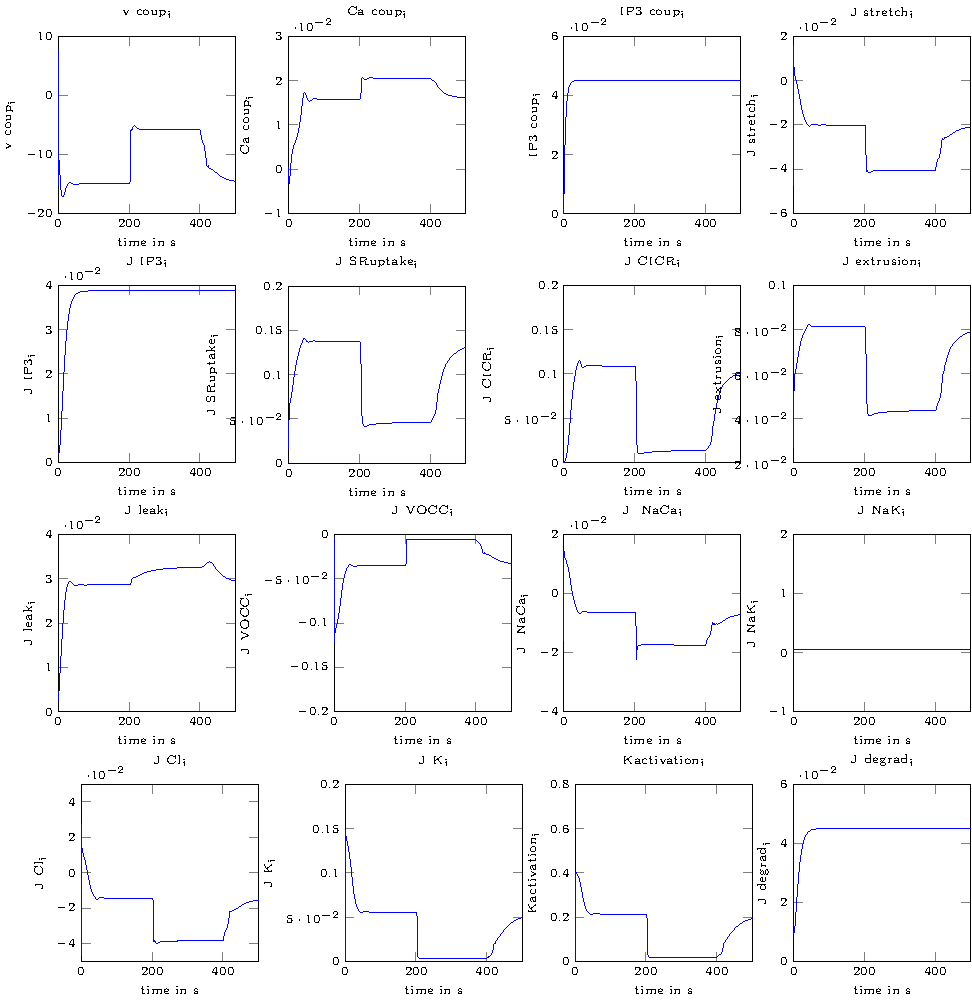
\includegraphics{figures/2_SMC_fluxes.pdf}
			\caption{The SMC fluxes}
			\label{fig:2SMCF}
		\end{figure}
		
		\begin{figure}[h!]
			\centering
			\tiny 
			\setlength\figureheight{3 cm} 
			\setlength\figurewidth{4.5 cm}
			%% % This file was created by matlab2tikz v0.3.3.
% Copyright (c) 2008--2013, Nico Schlömer <nico.schloemer@gmail.com>
% All rights reserved.
% 
% The latest updates can be retrieved from
%   http://www.mathworks.com/matlabcentral/fileexchange/22022-matlab2tikz
% where you can also make suggestions and rate matlab2tikz.
% 
% 
% 
\begin{tikzpicture}

\begin{axis}[%
width=\figurewidth,
height=\figureheight,
scale only axis,
xmin=0,
xmax=500,
xlabel={time in s},
ymin=0,
ymax=0.2,
ylabel={$\text{J}_\text{ }\text{IP3}_\text{j}$},
name=plot5,
title={$\text{J}_\text{ }\text{IP3}_\text{j}$}
]
\addplot [
color=blue,
solid,
forget plot
]
table[row sep=crcr]{
0 0.0022772\\
0.0011996 0.0022864\\
0.0023992 0.0022957\\
0.0035988 0.0023049\\
0.0085566 0.0023432\\
0.013514 0.0023819\\
0.018472 0.0024208\\
0.02343 0.0024599\\
0.033542 0.0025407\\
0.043655 0.0026226\\
0.053767 0.0027056\\
0.063879 0.0027897\\
0.073991 0.0028749\\
0.084819 0.0029674\\
0.095647 0.0030612\\
0.10647 0.0031561\\
0.1173 0.0032523\\
0.12813 0.0033497\\
0.14659 0.0035186\\
0.16505 0.0036909\\
0.18351 0.0038666\\
0.20197 0.0040457\\
0.22042 0.0042281\\
0.26398 0.0046713\\
0.30753 0.0051321\\
0.35108 0.0056097\\
0.37397 0.0058673\\
0.38969 0.0060466\\
0.4054 0.006228\\
0.42111 0.0064114\\
0.43393 0.0065626\\
0.44676 0.0067151\\
0.45959 0.0068689\\
0.47242 0.007024\\
0.48525 0.0071803\\
0.50035 0.0073659\\
0.51544 0.0075532\\
0.53054 0.0077422\\
0.54564 0.0079328\\
0.56073 0.008125\\
0.57728 0.0083375\\
0.59382 0.0085519\\
0.61036 0.0087681\\
0.6269 0.0089861\\
0.64344 0.0092059\\
0.65998 0.0094275\\
0.69992 0.0099696\\
0.73986 0.010521\\
0.77979 0.011082\\
0.81973 0.011652\\
0.85967 0.01223\\
0.99616 0.014265\\
1.1327 0.016378\\
1.2692 0.018556\\
1.4056 0.020785\\
1.6062 0.024129\\
1.8067 0.027525\\
2.0072 0.030945\\
2.2078 0.034366\\
2.4083 0.037765\\
2.8551 0.045187\\
3.302 0.052296\\
3.7488 0.059014\\
4.1956 0.065304\\
4.6425 0.071155\\
5.3586 0.079639\\
6.0748 0.087095\\
6.791 0.093631\\
7.5072 0.099358\\
8.2234 0.10438\\
9.2234 0.1104\\
10.223 0.11545\\
11.223 0.11971\\
12.223 0.12333\\
12.523 0.12431\\
12.823 0.12524\\
13.123 0.12613\\
13.423 0.12698\\
13.513 0.12723\\
13.603 0.12748\\
13.693 0.12772\\
13.783 0.12796\\
13.873 0.12819\\
13.929 0.12833\\
13.948 0.12838\\
13.967 0.12843\\
13.986 0.12848\\
14.004 0.12853\\
14.023 0.12857\\
14.079 0.12871\\
14.134 0.12885\\
14.189 0.12899\\
14.244 0.12912\\
14.299 0.12926\\
14.354 0.12939\\
14.409 0.12952\\
14.465 0.12966\\
14.52 0.12979\\
14.575 0.12992\\
14.631 0.13004\\
14.686 0.13017\\
14.742 0.1303\\
14.811 0.13046\\
14.88 0.13061\\
14.95 0.13077\\
15.019 0.13092\\
15.089 0.13107\\
15.202 0.13131\\
15.315 0.13155\\
15.428 0.13179\\
15.541 0.13202\\
15.654 0.13224\\
15.804 0.13254\\
15.954 0.13283\\
16.104 0.13312\\
16.255 0.13339\\
16.405 0.13367\\
16.675 0.13414\\
16.946 0.1346\\
17.216 0.13505\\
17.487 0.13547\\
17.757 0.13588\\
18.061 0.13633\\
18.364 0.13675\\
18.667 0.13716\\
18.971 0.13756\\
19.274 0.13794\\
19.375 0.13806\\
19.476 0.13818\\
19.576 0.1383\\
19.677 0.13842\\
19.778 0.13853\\
19.938 0.13871\\
20.097 0.13889\\
20.257 0.13906\\
20.416 0.13923\\
20.576 0.1394\\
20.994 0.13982\\
21.411 0.14022\\
21.828 0.1406\\
22.056 0.1408\\
22.119 0.14086\\
22.183 0.14091\\
22.247 0.14096\\
22.31 0.14102\\
22.432 0.14112\\
22.554 0.14122\\
22.676 0.14132\\
22.798 0.14141\\
22.92 0.14151\\
23.367 0.14184\\
23.684 0.14207\\
24 0.14229\\
24.242 0.14246\\
24.484 0.14261\\
24.726 0.14277\\
24.968 0.14292\\
25.298 0.14311\\
25.628 0.1433\\
25.958 0.14348\\
26.288 0.14366\\
26.618 0.14383\\
27.087 0.14406\\
27.556 0.14428\\
28.025 0.14448\\
28.494 0.14468\\
28.964 0.14486\\
29.615 0.14511\\
30.266 0.14533\\
30.917 0.14554\\
31.569 0.14574\\
32.372 0.14596\\
33.175 0.14617\\
33.979 0.14635\\
34.782 0.14653\\
35.586 0.14668\\
36.23 0.1468\\
36.875 0.14691\\
37.52 0.14701\\
38.164 0.14711\\
38.969 0.14722\\
39.774 0.14732\\
40.579 0.14741\\
41.384 0.1475\\
42.189 0.14758\\
43.189 0.14767\\
44.189 0.14775\\
45.189 0.14782\\
46.189 0.14789\\
47.189 0.14795\\
48.189 0.148\\
49.189 0.14805\\
50.189 0.1481\\
51.189 0.14814\\
52.189 0.14817\\
53.189 0.14821\\
54.189 0.14823\\
55.189 0.14826\\
56.189 0.14829\\
57.189 0.14831\\
58.189 0.14833\\
59.189 0.14834\\
60.189 0.14836\\
61.189 0.14837\\
62.189 0.14839\\
63.189 0.1484\\
64.189 0.14841\\
65.189 0.14842\\
66.189 0.14843\\
67.189 0.14844\\
68.189 0.14844\\
69.189 0.14845\\
70.189 0.14846\\
71.189 0.14846\\
72.189 0.14847\\
73.189 0.14847\\
74.189 0.14847\\
75.189 0.14848\\
76.189 0.14848\\
77.189 0.14848\\
78.189 0.14849\\
79.189 0.14849\\
80.189 0.14849\\
81.189 0.14849\\
82.189 0.14849\\
83.189 0.1485\\
84.189 0.1485\\
85.189 0.1485\\
86.189 0.1485\\
87.189 0.1485\\
88.189 0.1485\\
89.189 0.1485\\
90.189 0.1485\\
91.189 0.1485\\
92.189 0.14851\\
93.189 0.14851\\
94.189 0.14851\\
95.189 0.14851\\
96.189 0.14851\\
97.189 0.14851\\
98.189 0.14851\\
99.189 0.14851\\
100.19 0.14851\\
101.19 0.14851\\
102.19 0.14851\\
103.19 0.14851\\
104.19 0.14851\\
105.19 0.14851\\
106.19 0.14851\\
107.19 0.14851\\
108.19 0.14851\\
109.19 0.14851\\
110.19 0.14851\\
111.19 0.14851\\
112.19 0.14851\\
113.19 0.14851\\
114.19 0.14851\\
115.19 0.14851\\
116.19 0.14851\\
117.19 0.14851\\
118.19 0.14851\\
119.19 0.14851\\
120.19 0.14851\\
121.19 0.14851\\
122.19 0.14851\\
123.19 0.14851\\
124.19 0.14851\\
125.19 0.14851\\
126.19 0.14851\\
127.19 0.14851\\
128.19 0.14851\\
129.19 0.14851\\
130.19 0.14851\\
131.19 0.14851\\
132.19 0.14851\\
133.19 0.14851\\
134.19 0.14851\\
135.19 0.14851\\
136.19 0.14851\\
137.19 0.14851\\
138.19 0.14851\\
139.19 0.14851\\
140.19 0.14851\\
141.19 0.14851\\
142.19 0.14851\\
143.19 0.14851\\
144.19 0.14851\\
145.19 0.14851\\
146.19 0.14851\\
147.19 0.14851\\
148.19 0.14851\\
149.19 0.14851\\
150.19 0.14851\\
151.19 0.14851\\
152.19 0.14851\\
153.19 0.14851\\
154.19 0.14851\\
155.19 0.14851\\
156.19 0.14851\\
157.19 0.14851\\
158.19 0.14851\\
159.19 0.14851\\
160.19 0.14851\\
161.19 0.14851\\
162.19 0.14851\\
163.19 0.14851\\
164.19 0.14851\\
165.19 0.14851\\
166.19 0.14851\\
167.19 0.14851\\
168.19 0.14851\\
169.19 0.14851\\
170.19 0.14851\\
171.19 0.14851\\
172.19 0.14851\\
173.19 0.14851\\
174.19 0.14851\\
175.19 0.14851\\
176.19 0.14851\\
177.19 0.14851\\
178.19 0.14851\\
179.19 0.14851\\
180.19 0.14851\\
181.19 0.14851\\
182.19 0.14851\\
183.19 0.14851\\
184.19 0.14851\\
185.19 0.14851\\
186.19 0.14851\\
187.19 0.14851\\
188.19 0.14851\\
189.19 0.14851\\
190.19 0.14851\\
191.19 0.14851\\
192.19 0.14851\\
193.19 0.14851\\
194.19 0.14851\\
195.19 0.14851\\
196.19 0.14851\\
196.81 0.14851\\
197.25 0.14851\\
197.57 0.14851\\
197.82 0.14851\\
198.03 0.14851\\
198.24 0.14851\\
198.38 0.14851\\
198.52 0.14851\\
198.63 0.14851\\
198.74 0.14851\\
198.83 0.14851\\
198.92 0.14851\\
199.01 0.14851\\
199.17 0.14851\\
199.32 0.14851\\
199.47 0.14851\\
199.62 0.14851\\
199.84 0.14851\\
200.07 0.14851\\
200.29 0.14851\\
200.51 0.14851\\
200.69 0.14851\\
200.87 0.14851\\
201.05 0.14851\\
201.23 0.14851\\
201.42 0.14851\\
201.6 0.14851\\
201.79 0.14851\\
201.97 0.14851\\
202.15 0.14851\\
202.34 0.14851\\
202.63 0.14851\\
202.92 0.14851\\
203.21 0.14851\\
203.5 0.14851\\
203.79 0.14851\\
204.09 0.14851\\
204.39 0.14851\\
204.69 0.14851\\
204.94 0.14851\\
205.19 0.14851\\
205.44 0.14851\\
205.68 0.14851\\
205.85 0.14851\\
206.02 0.14851\\
206.19 0.14851\\
206.36 0.14851\\
206.6 0.14851\\
206.84 0.14851\\
207.08 0.14851\\
207.32 0.14851\\
207.65 0.14851\\
207.99 0.14851\\
208.32 0.14851\\
208.65 0.14851\\
208.99 0.14851\\
209.66 0.14851\\
210.18 0.14851\\
210.7 0.14851\\
211.22 0.14851\\
211.74 0.14851\\
212.26 0.14851\\
212.9 0.14851\\
213.54 0.14851\\
214.18 0.14851\\
214.82 0.14851\\
215.46 0.14851\\
216.16 0.14851\\
216.87 0.14851\\
217.57 0.14851\\
218.27 0.14851\\
218.98 0.14851\\
219.98 0.14851\\
220.98 0.14851\\
221.98 0.14851\\
222.98 0.14851\\
223.98 0.14851\\
224.98 0.14851\\
225.98 0.14851\\
226.98 0.14851\\
227.98 0.14851\\
228.98 0.14851\\
229.98 0.14851\\
230.98 0.14851\\
231.98 0.14851\\
232.98 0.14851\\
233.98 0.14851\\
234.98 0.14851\\
235.98 0.14851\\
236.98 0.14851\\
237.98 0.14851\\
238.98 0.14851\\
239.98 0.14851\\
240.98 0.14851\\
241.98 0.14851\\
242.98 0.14851\\
243.98 0.14851\\
244.98 0.14851\\
245.98 0.14851\\
246.98 0.14851\\
247.98 0.14851\\
248.98 0.14851\\
249.98 0.14851\\
250.98 0.14851\\
251.98 0.14851\\
252.98 0.14851\\
253.98 0.14851\\
254.98 0.14851\\
255.98 0.14851\\
256.98 0.14851\\
257.98 0.14851\\
258.98 0.14851\\
259.98 0.14851\\
260.98 0.14851\\
261.98 0.14851\\
262.98 0.14851\\
263.98 0.14851\\
264.98 0.14851\\
265.98 0.14851\\
266.98 0.14851\\
267.98 0.14851\\
268.98 0.14851\\
269.98 0.14851\\
270.98 0.14851\\
271.98 0.14851\\
272.98 0.14851\\
273.98 0.14851\\
274.98 0.14851\\
275.98 0.14851\\
276.98 0.14851\\
277.98 0.14851\\
278.98 0.14851\\
279.98 0.14851\\
280.98 0.14851\\
281.98 0.14851\\
282.98 0.14851\\
283.98 0.14851\\
284.98 0.14851\\
285.98 0.14851\\
286.98 0.14851\\
287.98 0.14851\\
288.98 0.14851\\
289.98 0.14851\\
290.98 0.14851\\
291.98 0.14851\\
292.98 0.14851\\
293.98 0.14851\\
294.98 0.14851\\
295.98 0.14851\\
296.98 0.14851\\
297.98 0.14851\\
298.98 0.14851\\
299.98 0.14851\\
300.98 0.14851\\
301.98 0.14851\\
302.98 0.14851\\
303.98 0.14851\\
304.98 0.14851\\
305.98 0.14851\\
306.98 0.14851\\
307.98 0.14851\\
308.98 0.14851\\
309.98 0.14851\\
310.98 0.14851\\
311.98 0.14851\\
312.98 0.14851\\
313.98 0.14851\\
314.98 0.14851\\
315.98 0.14851\\
316.98 0.14851\\
317.98 0.14851\\
318.98 0.14851\\
319.98 0.14851\\
320.98 0.14851\\
321.98 0.14851\\
322.98 0.14851\\
323.98 0.14851\\
324.98 0.14851\\
325.98 0.14851\\
326.98 0.14851\\
327.98 0.14851\\
328.98 0.14851\\
329.98 0.14851\\
330.98 0.14851\\
331.98 0.14851\\
332.98 0.14851\\
333.98 0.14851\\
334.98 0.14851\\
335.98 0.14851\\
336.98 0.14851\\
337.98 0.14851\\
338.98 0.14851\\
339.98 0.14851\\
340.98 0.14851\\
341.98 0.14851\\
342.98 0.14851\\
343.98 0.14851\\
344.98 0.14851\\
345.98 0.14851\\
346.98 0.14851\\
347.98 0.14851\\
348.98 0.14851\\
349.98 0.14851\\
350.98 0.14851\\
351.98 0.14851\\
352.98 0.14851\\
353.98 0.14851\\
354.98 0.14851\\
355.98 0.14851\\
356.98 0.14851\\
357.98 0.14851\\
358.98 0.14851\\
359.98 0.14851\\
360.98 0.14851\\
361.98 0.14851\\
362.98 0.14851\\
363.98 0.14851\\
364.98 0.14851\\
365.98 0.14851\\
366.98 0.14851\\
367.98 0.14851\\
368.98 0.14851\\
369.98 0.14851\\
370.98 0.14851\\
371.98 0.14851\\
372.98 0.14851\\
373.98 0.14851\\
374.98 0.14851\\
375.98 0.14851\\
376.98 0.14851\\
377.98 0.14851\\
378.98 0.14851\\
379.98 0.14851\\
380.98 0.14851\\
381.98 0.14851\\
382.98 0.14851\\
383.98 0.14851\\
384.98 0.14851\\
385.98 0.14851\\
386.98 0.14851\\
387.98 0.14851\\
388.98 0.14851\\
389.98 0.14851\\
390.98 0.14851\\
391.98 0.14851\\
392.98 0.14851\\
393.98 0.14851\\
394.98 0.14851\\
395.98 0.14851\\
396.98 0.14851\\
397.98 0.14851\\
398.44 0.14851\\
398.8 0.14851\\
399.07 0.14851\\
399.35 0.14851\\
399.55 0.14851\\
399.76 0.14851\\
399.96 0.14851\\
400.26 0.14851\\
400.34 0.14851\\
400.43 0.14851\\
400.52 0.14851\\
400.61 0.14851\\
400.92 0.14851\\
401.24 0.14851\\
401.56 0.14851\\
401.87 0.14851\\
402.11 0.14851\\
402.35 0.14851\\
402.59 0.14851\\
402.83 0.14851\\
403.14 0.14851\\
403.45 0.14851\\
403.77 0.14851\\
404.08 0.14851\\
404.39 0.14851\\
404.93 0.14851\\
405.47 0.14851\\
406.02 0.14851\\
406.56 0.14851\\
407.1 0.14851\\
408.1 0.14851\\
408.77 0.14851\\
409.43 0.14851\\
410.1 0.14851\\
410.61 0.14851\\
411.12 0.14851\\
411.63 0.14851\\
412.15 0.14851\\
412.66 0.14851\\
413.31 0.14851\\
413.95 0.14851\\
414.6 0.14851\\
415.25 0.14851\\
415.9 0.14851\\
416.77 0.14851\\
417.65 0.14851\\
418.52 0.14851\\
419.4 0.14851\\
420.28 0.14851\\
421.2 0.14851\\
422.12 0.14851\\
423.04 0.14851\\
423.96 0.14851\\
424.89 0.14851\\
425.81 0.14851\\
426.73 0.14851\\
427.68 0.14851\\
428.64 0.14851\\
429.59 0.14851\\
430.55 0.14851\\
431.5 0.14851\\
432.5 0.14851\\
433.5 0.14851\\
434.5 0.14851\\
435.5 0.14851\\
436.5 0.14851\\
437.5 0.14851\\
438.5 0.14851\\
439.5 0.14851\\
440.5 0.14851\\
441.5 0.14851\\
442.5 0.14851\\
443.5 0.14851\\
444.5 0.14851\\
445.5 0.14851\\
446.5 0.14851\\
447.5 0.14851\\
448.5 0.14851\\
449.5 0.14851\\
450.5 0.14851\\
451.5 0.14851\\
452.5 0.14851\\
453.5 0.14851\\
454.5 0.14851\\
455.5 0.14851\\
456.5 0.14851\\
457.5 0.14851\\
458.5 0.14851\\
459.5 0.14851\\
460.5 0.14851\\
461.5 0.14851\\
462.5 0.14851\\
463.5 0.14851\\
464.5 0.14851\\
465.5 0.14851\\
466.5 0.14851\\
467.5 0.14851\\
468.5 0.14851\\
469.5 0.14851\\
470.5 0.14851\\
471.5 0.14851\\
472.5 0.14851\\
473.5 0.14851\\
474.5 0.14851\\
475.5 0.14851\\
476.5 0.14851\\
477.5 0.14851\\
478.5 0.14851\\
479.5 0.14851\\
480.5 0.14851\\
481.5 0.14851\\
482.5 0.14851\\
483.5 0.14851\\
484.5 0.14851\\
485.5 0.14851\\
486.5 0.14851\\
487.5 0.14851\\
488.5 0.14851\\
489.5 0.14851\\
490.5 0.14851\\
491.5 0.14851\\
492.5 0.14851\\
493.5 0.14851\\
494.5 0.14851\\
495.5 0.14851\\
496.5 0.14851\\
497.5 0.14851\\
498.5 0.14851\\
499.5 0.14851\\
500 0.14851\\
};
\end{axis}

\begin{axis}[%
width=\figurewidth,
height=\figureheight,
scale only axis,
xmin=0,
xmax=500,
xlabel={time in s},
ymin=-0.03,
ymax=0.01,
ylabel={$\text{Ca}_\text{ }\text{coup}_\text{j}$},
name=plot2,
at=(plot5.above north west),
anchor=below south west,
title={$\text{Ca}_\text{ }\text{coup}_\text{j}$}
]
\addplot [
color=blue,
solid,
forget plot
]
table[row sep=crcr]{
0 -0\\
0.0011996 -2.2127e-07\\
0.0023992 -5.5314e-07\\
0.0035988 -9.9233e-07\\
0.0085566 -3.7299e-06\\
0.013514 -7.8673e-06\\
0.018472 -1.3155e-05\\
0.02343 -1.9356e-05\\
0.033542 -3.4093e-05\\
0.043655 -5.054e-05\\
0.053767 -6.7812e-05\\
0.063879 -8.537e-05\\
0.073991 -0.00010287\\
0.084819 -0.00012129\\
0.095647 -0.00013918\\
0.10647 -0.00015638\\
0.1173 -0.00017282\\
0.12813 -0.00018841\\
0.14659 -0.00021289\\
0.16505 -0.00023447\\
0.18351 -0.0002529\\
0.20197 -0.00026787\\
0.22042 -0.00027899\\
0.26398 -0.00028604\\
0.30753 -0.00025576\\
0.35108 -0.00016851\\
0.37397 -9.3924e-05\\
0.38969 -3.1601e-05\\
0.4054 3.7242e-05\\
0.42111 0.00011002\\
0.43393 0.00017085\\
0.44676 0.00023209\\
0.45959 0.00029329\\
0.47242 0.00035418\\
0.48525 0.0004146\\
0.50035 0.00048497\\
0.51544 0.00055445\\
0.53054 0.00062298\\
0.54564 0.00069052\\
0.56073 0.00075706\\
0.57728 0.00082881\\
0.59382 0.00089935\\
0.61036 0.00096868\\
0.6269 0.0010368\\
0.64344 0.0011038\\
0.65998 0.0011695\\
0.69992 0.0013235\\
0.73986 0.0014706\\
0.77979 0.0016111\\
0.81973 0.001745\\
0.85967 0.0018724\\
0.99616 0.0022614\\
1.1327 0.0025817\\
1.2692 0.002839\\
1.4056 0.0030393\\
1.6062 0.0032423\\
1.8067 0.003353\\
2.0072 0.0033884\\
2.2078 0.003363\\
2.4083 0.0032886\\
2.8551 0.0029914\\
3.302 0.002579\\
3.7488 0.0021043\\
4.1956 0.0015996\\
4.6425 0.0010859\\
5.3586 0.0002766\\
6.0748 -0.00048183\\
6.791 -0.0011728\\
7.5072 -0.0017928\\
8.2234 -0.0023442\\
9.2234 -0.0030094\\
10.223 -0.0035654\\
11.223 -0.0040271\\
12.223 -0.0044129\\
12.523 -0.0045171\\
12.823 -0.0046171\\
13.123 -0.0047128\\
13.423 -0.0048041\\
13.513 -0.0048307\\
13.603 -0.004857\\
13.693 -0.0048829\\
13.783 -0.0049085\\
13.873 -0.0049339\\
13.929 -0.0049493\\
13.948 -0.0049546\\
13.967 -0.0049598\\
13.986 -0.004965\\
14.004 -0.0049703\\
14.023 -0.0049755\\
14.079 -0.0049905\\
14.134 -0.0050055\\
14.189 -0.0050204\\
14.244 -0.0050352\\
14.299 -0.0050498\\
14.354 -0.0050644\\
14.409 -0.0050789\\
14.465 -0.0050933\\
14.52 -0.0051077\\
14.575 -0.005122\\
14.631 -0.0051362\\
14.686 -0.0051503\\
14.742 -0.0051643\\
14.811 -0.0051818\\
14.88 -0.0051992\\
14.95 -0.0052164\\
15.019 -0.0052335\\
15.089 -0.0052505\\
15.202 -0.005278\\
15.315 -0.0053051\\
15.428 -0.005332\\
15.541 -0.0053587\\
15.654 -0.0053851\\
15.804 -0.00542\\
15.954 -0.0054544\\
16.104 -0.0054886\\
16.255 -0.0055224\\
16.405 -0.0055559\\
16.675 -0.0056157\\
16.946 -0.0056749\\
17.216 -0.0057336\\
17.487 -0.0057919\\
17.757 -0.0058501\\
18.061 -0.0059153\\
18.364 -0.0059805\\
18.667 -0.006046\\
18.971 -0.0061118\\
19.274 -0.0061782\\
19.375 -0.0062004\\
19.476 -0.0062227\\
19.576 -0.006245\\
19.677 -0.0062675\\
19.778 -0.00629\\
19.938 -0.0063258\\
20.097 -0.006362\\
20.257 -0.0063983\\
20.416 -0.006435\\
20.576 -0.0064719\\
20.994 -0.0065699\\
21.411 -0.0066702\\
21.828 -0.0067728\\
22.056 -0.0068297\\
22.119 -0.0068458\\
22.183 -0.0068619\\
22.247 -0.0068782\\
22.31 -0.0068944\\
22.432 -0.0069257\\
22.554 -0.0069573\\
22.676 -0.0069891\\
22.798 -0.0070211\\
22.92 -0.0070534\\
23.367 -0.007174\\
23.684 -0.0072615\\
24 -0.0073508\\
24.242 -0.0074203\\
24.484 -0.0074909\\
24.726 -0.0075627\\
24.968 -0.0076356\\
25.298 -0.007737\\
25.628 -0.0078407\\
25.958 -0.0079467\\
26.288 -0.0080552\\
26.618 -0.0081663\\
27.087 -0.0083287\\
27.556 -0.0084967\\
28.025 -0.0086705\\
28.494 -0.0088503\\
28.964 -0.0090365\\
29.615 -0.0093061\\
30.266 -0.0095893\\
30.917 -0.0098867\\
31.569 -0.010199\\
32.372 -0.010606\\
33.175 -0.011037\\
33.979 -0.011494\\
34.782 -0.011975\\
35.586 -0.01248\\
36.23 -0.012899\\
36.875 -0.013328\\
37.52 -0.013764\\
38.164 -0.014203\\
38.969 -0.014745\\
39.774 -0.01527\\
40.579 -0.015761\\
41.384 -0.016204\\
42.189 -0.016583\\
43.189 -0.016948\\
44.189 -0.017188\\
45.189 -0.017301\\
46.189 -0.017301\\
47.189 -0.017207\\
48.189 -0.017043\\
49.189 -0.016832\\
50.189 -0.016599\\
51.189 -0.01636\\
52.189 -0.016128\\
53.189 -0.015916\\
54.189 -0.015731\\
55.189 -0.015578\\
56.189 -0.01546\\
57.189 -0.015377\\
58.189 -0.015327\\
59.189 -0.015308\\
60.189 -0.015315\\
61.189 -0.015343\\
62.189 -0.015388\\
63.189 -0.015444\\
64.189 -0.015509\\
65.189 -0.015576\\
66.189 -0.015643\\
67.189 -0.015707\\
68.189 -0.015764\\
69.189 -0.01581\\
70.189 -0.015846\\
71.189 -0.015872\\
72.189 -0.015891\\
73.189 -0.015901\\
74.189 -0.015904\\
75.189 -0.0159\\
76.189 -0.015889\\
77.189 -0.015875\\
78.189 -0.015859\\
79.189 -0.015843\\
80.189 -0.015826\\
81.189 -0.01581\\
82.189 -0.015796\\
83.189 -0.015784\\
84.189 -0.015774\\
85.189 -0.015766\\
86.189 -0.015761\\
87.189 -0.015758\\
88.189 -0.015757\\
89.189 -0.015758\\
90.189 -0.01576\\
91.189 -0.015764\\
92.189 -0.015768\\
93.189 -0.015773\\
94.189 -0.015777\\
95.189 -0.015782\\
96.189 -0.015786\\
97.189 -0.01579\\
98.189 -0.015793\\
99.189 -0.015795\\
100.19 -0.015797\\
101.19 -0.015799\\
102.19 -0.015799\\
103.19 -0.0158\\
104.19 -0.0158\\
105.19 -0.015799\\
106.19 -0.015798\\
107.19 -0.015798\\
108.19 -0.015797\\
109.19 -0.015796\\
110.19 -0.015795\\
111.19 -0.015794\\
112.19 -0.015794\\
113.19 -0.015793\\
114.19 -0.015793\\
115.19 -0.015793\\
116.19 -0.015793\\
117.19 -0.015793\\
118.19 -0.015793\\
119.19 -0.015794\\
120.19 -0.015794\\
121.19 -0.015794\\
122.19 -0.015795\\
123.19 -0.015795\\
124.19 -0.015796\\
125.19 -0.015796\\
126.19 -0.015796\\
127.19 -0.015796\\
128.19 -0.015797\\
129.19 -0.015797\\
130.19 -0.015797\\
131.19 -0.015797\\
132.19 -0.015797\\
133.19 -0.015797\\
134.19 -0.015797\\
135.19 -0.015798\\
136.19 -0.015798\\
137.19 -0.015798\\
138.19 -0.015798\\
139.19 -0.015798\\
140.19 -0.015798\\
141.19 -0.015798\\
142.19 -0.015798\\
143.19 -0.015798\\
144.19 -0.015798\\
145.19 -0.015798\\
146.19 -0.015798\\
147.19 -0.015798\\
148.19 -0.015798\\
149.19 -0.015798\\
150.19 -0.015799\\
151.19 -0.015799\\
152.19 -0.015799\\
153.19 -0.015799\\
154.19 -0.015799\\
155.19 -0.015799\\
156.19 -0.015799\\
157.19 -0.015799\\
158.19 -0.015799\\
159.19 -0.015799\\
160.19 -0.015799\\
161.19 -0.015799\\
162.19 -0.015799\\
163.19 -0.015799\\
164.19 -0.015799\\
165.19 -0.015799\\
166.19 -0.0158\\
167.19 -0.0158\\
168.19 -0.0158\\
169.19 -0.0158\\
170.19 -0.0158\\
171.19 -0.0158\\
172.19 -0.0158\\
173.19 -0.0158\\
174.19 -0.0158\\
175.19 -0.0158\\
176.19 -0.0158\\
177.19 -0.0158\\
178.19 -0.0158\\
179.19 -0.0158\\
180.19 -0.0158\\
181.19 -0.0158\\
182.19 -0.0158\\
183.19 -0.0158\\
184.19 -0.0158\\
185.19 -0.0158\\
186.19 -0.0158\\
187.19 -0.0158\\
188.19 -0.015801\\
189.19 -0.015801\\
190.19 -0.015801\\
191.19 -0.015801\\
192.19 -0.015801\\
193.19 -0.015801\\
194.19 -0.015801\\
195.19 -0.015801\\
196.19 -0.015801\\
196.81 -0.015801\\
197.25 -0.015801\\
197.57 -0.015801\\
197.82 -0.015801\\
198.03 -0.015801\\
198.24 -0.015801\\
198.38 -0.015801\\
198.52 -0.015801\\
198.63 -0.015801\\
198.74 -0.015801\\
198.83 -0.015801\\
198.92 -0.015801\\
199.01 -0.015801\\
199.17 -0.015801\\
199.32 -0.015801\\
199.47 -0.015801\\
199.62 -0.015801\\
199.84 -0.015801\\
200.07 -0.015801\\
200.29 -0.015801\\
200.51 -0.015801\\
200.69 -0.015801\\
200.87 -0.015801\\
201.05 -0.015801\\
201.23 -0.015802\\
201.42 -0.015802\\
201.6 -0.015804\\
201.79 -0.015806\\
201.97 -0.01581\\
202.15 -0.015815\\
202.34 -0.015823\\
202.63 -0.015844\\
202.92 -0.01588\\
203.21 -0.015939\\
203.5 -0.016035\\
203.79 -0.016183\\
204.09 -0.016412\\
204.39 -0.016739\\
204.69 -0.017171\\
204.94 -0.017598\\
205.19 -0.018062\\
205.44 -0.018525\\
205.68 -0.018948\\
205.85 -0.019207\\
206.02 -0.019438\\
206.19 -0.019642\\
206.36 -0.019821\\
206.6 -0.020036\\
206.84 -0.020209\\
207.08 -0.020346\\
207.32 -0.020453\\
207.65 -0.020559\\
207.99 -0.020626\\
208.32 -0.020665\\
208.65 -0.020681\\
208.99 -0.02068\\
209.66 -0.020642\\
210.18 -0.020594\\
210.7 -0.020538\\
211.22 -0.020479\\
211.74 -0.020419\\
212.26 -0.020363\\
212.9 -0.020299\\
213.54 -0.020245\\
214.18 -0.0202\\
214.82 -0.020166\\
215.46 -0.020141\\
216.16 -0.020127\\
216.87 -0.020123\\
217.57 -0.02013\\
218.27 -0.020146\\
218.98 -0.02017\\
219.98 -0.020215\\
220.98 -0.02027\\
221.98 -0.020331\\
222.98 -0.020395\\
223.98 -0.020458\\
224.98 -0.020517\\
225.98 -0.02057\\
226.98 -0.020615\\
227.98 -0.020651\\
228.98 -0.020678\\
229.98 -0.020694\\
230.98 -0.020701\\
231.98 -0.0207\\
232.98 -0.02069\\
233.98 -0.020675\\
234.98 -0.020655\\
235.98 -0.020632\\
236.98 -0.020606\\
237.98 -0.020581\\
238.98 -0.020556\\
239.98 -0.020533\\
240.98 -0.020513\\
241.98 -0.020495\\
242.98 -0.020481\\
243.98 -0.020469\\
244.98 -0.02046\\
245.98 -0.020453\\
246.98 -0.020449\\
247.98 -0.020447\\
248.98 -0.020447\\
249.98 -0.020448\\
250.98 -0.02045\\
251.98 -0.020452\\
252.98 -0.020455\\
253.98 -0.020458\\
254.98 -0.02046\\
255.98 -0.020463\\
256.98 -0.020464\\
257.98 -0.020466\\
258.98 -0.020466\\
259.98 -0.020466\\
260.98 -0.020466\\
261.98 -0.020465\\
262.98 -0.020463\\
263.98 -0.020461\\
264.98 -0.020459\\
265.98 -0.020456\\
266.98 -0.020453\\
267.98 -0.02045\\
268.98 -0.020447\\
269.98 -0.020445\\
270.98 -0.020442\\
271.98 -0.020439\\
272.98 -0.020437\\
273.98 -0.020435\\
274.98 -0.020432\\
275.98 -0.02043\\
276.98 -0.020429\\
277.98 -0.020427\\
278.98 -0.020426\\
279.98 -0.020425\\
280.98 -0.020423\\
281.98 -0.020422\\
282.98 -0.020421\\
283.98 -0.02042\\
284.98 -0.02042\\
285.98 -0.020419\\
286.98 -0.020418\\
287.98 -0.020417\\
288.98 -0.020416\\
289.98 -0.020415\\
290.98 -0.020414\\
291.98 -0.020413\\
292.98 -0.020413\\
293.98 -0.020412\\
294.98 -0.020411\\
295.98 -0.02041\\
296.98 -0.020409\\
297.98 -0.020408\\
298.98 -0.020407\\
299.98 -0.020406\\
300.98 -0.020405\\
301.98 -0.020404\\
302.98 -0.020404\\
303.98 -0.020403\\
304.98 -0.020402\\
305.98 -0.020401\\
306.98 -0.0204\\
307.98 -0.0204\\
308.98 -0.020399\\
309.98 -0.020398\\
310.98 -0.020398\\
311.98 -0.020397\\
312.98 -0.020396\\
313.98 -0.020396\\
314.98 -0.020395\\
315.98 -0.020395\\
316.98 -0.020394\\
317.98 -0.020394\\
318.98 -0.020393\\
319.98 -0.020393\\
320.98 -0.020392\\
321.98 -0.020392\\
322.98 -0.020391\\
323.98 -0.020391\\
324.98 -0.02039\\
325.98 -0.02039\\
326.98 -0.020389\\
327.98 -0.020389\\
328.98 -0.020388\\
329.98 -0.020388\\
330.98 -0.020387\\
331.98 -0.020387\\
332.98 -0.020387\\
333.98 -0.020386\\
334.98 -0.020386\\
335.98 -0.020386\\
336.98 -0.020385\\
337.98 -0.020385\\
338.98 -0.020384\\
339.98 -0.020384\\
340.98 -0.020384\\
341.98 -0.020384\\
342.98 -0.020383\\
343.98 -0.020383\\
344.98 -0.020383\\
345.98 -0.020382\\
346.98 -0.020382\\
347.98 -0.020382\\
348.98 -0.020381\\
349.98 -0.020381\\
350.98 -0.020381\\
351.98 -0.020381\\
352.98 -0.02038\\
353.98 -0.02038\\
354.98 -0.02038\\
355.98 -0.02038\\
356.98 -0.02038\\
357.98 -0.020379\\
358.98 -0.020379\\
359.98 -0.020379\\
360.98 -0.020379\\
361.98 -0.020379\\
362.98 -0.020378\\
363.98 -0.020378\\
364.98 -0.020378\\
365.98 -0.020378\\
366.98 -0.020378\\
367.98 -0.020377\\
368.98 -0.020377\\
369.98 -0.020377\\
370.98 -0.020377\\
371.98 -0.020377\\
372.98 -0.020377\\
373.98 -0.020376\\
374.98 -0.020376\\
375.98 -0.020376\\
376.98 -0.020376\\
377.98 -0.020376\\
378.98 -0.020376\\
379.98 -0.020376\\
380.98 -0.020376\\
381.98 -0.020375\\
382.98 -0.020375\\
383.98 -0.020375\\
384.98 -0.020375\\
385.98 -0.020375\\
386.98 -0.020375\\
387.98 -0.020375\\
388.98 -0.020375\\
389.98 -0.020375\\
390.98 -0.020374\\
391.98 -0.020374\\
392.98 -0.020374\\
393.98 -0.020374\\
394.98 -0.020374\\
395.98 -0.020374\\
396.98 -0.020374\\
397.98 -0.020374\\
398.44 -0.020374\\
398.8 -0.020374\\
399.07 -0.020374\\
399.35 -0.020374\\
399.55 -0.020374\\
399.76 -0.020374\\
399.96 -0.020374\\
400.26 -0.020373\\
400.34 -0.020373\\
400.43 -0.020373\\
400.52 -0.020372\\
400.61 -0.020371\\
400.92 -0.020367\\
401.24 -0.020359\\
401.56 -0.020349\\
401.87 -0.020336\\
402.11 -0.020325\\
402.35 -0.020313\\
402.59 -0.020299\\
402.83 -0.020285\\
403.14 -0.020266\\
403.45 -0.020247\\
403.77 -0.020227\\
404.08 -0.020206\\
404.39 -0.020186\\
404.93 -0.020151\\
405.47 -0.020117\\
406.02 -0.020085\\
406.56 -0.020055\\
407.1 -0.020028\\
408.1 -0.019984\\
408.77 -0.01996\\
409.43 -0.01994\\
410.1 -0.019925\\
410.61 -0.019914\\
411.12 -0.019902\\
411.63 -0.019886\\
412.15 -0.019864\\
412.66 -0.019837\\
413.31 -0.019795\\
413.95 -0.019745\\
414.6 -0.019685\\
415.25 -0.019616\\
415.9 -0.019537\\
416.77 -0.01941\\
417.65 -0.019259\\
418.52 -0.01908\\
419.4 -0.018881\\
420.28 -0.018683\\
421.2 -0.018514\\
422.12 -0.018413\\
423.04 -0.018371\\
423.96 -0.018347\\
424.89 -0.018297\\
425.81 -0.01821\\
426.73 -0.018111\\
427.68 -0.018021\\
428.64 -0.01795\\
429.59 -0.017886\\
430.55 -0.017813\\
431.5 -0.017731\\
432.5 -0.017643\\
433.5 -0.01756\\
434.5 -0.017486\\
435.5 -0.017415\\
436.5 -0.017344\\
437.5 -0.017273\\
438.5 -0.017207\\
439.5 -0.017148\\
440.5 -0.017095\\
441.5 -0.017045\\
442.5 -0.016999\\
443.5 -0.016958\\
444.5 -0.01692\\
445.5 -0.016886\\
446.5 -0.016853\\
447.5 -0.016823\\
448.5 -0.016794\\
449.5 -0.016767\\
450.5 -0.016741\\
451.5 -0.016717\\
452.5 -0.016693\\
453.5 -0.016671\\
454.5 -0.016649\\
455.5 -0.016627\\
456.5 -0.016607\\
457.5 -0.016586\\
458.5 -0.016566\\
459.5 -0.016547\\
460.5 -0.016527\\
461.5 -0.016509\\
462.5 -0.016491\\
463.5 -0.016473\\
464.5 -0.016456\\
465.5 -0.016439\\
466.5 -0.016423\\
467.5 -0.016407\\
468.5 -0.016392\\
469.5 -0.016377\\
470.5 -0.016363\\
471.5 -0.016349\\
472.5 -0.016336\\
473.5 -0.016323\\
474.5 -0.016311\\
475.5 -0.016298\\
476.5 -0.016287\\
477.5 -0.016275\\
478.5 -0.016264\\
479.5 -0.016253\\
480.5 -0.016242\\
481.5 -0.016232\\
482.5 -0.016222\\
483.5 -0.016212\\
484.5 -0.016202\\
485.5 -0.016193\\
486.5 -0.016184\\
487.5 -0.016175\\
488.5 -0.016166\\
489.5 -0.016158\\
490.5 -0.016149\\
491.5 -0.016141\\
492.5 -0.016133\\
493.5 -0.016126\\
494.5 -0.016118\\
495.5 -0.016111\\
496.5 -0.016104\\
497.5 -0.016097\\
498.5 -0.01609\\
499.5 -0.016084\\
500 -0.016081\\
};
\end{axis}

\begin{axis}[%
width=\figurewidth,
height=\figureheight,
scale only axis,
xmin=0,
xmax=500,
xlabel={time in s},
ymin=-10,
ymax=20,
ylabel={$\text{v}_\text{ }\text{coup}_\text{j}$},
name=plot1,
at=(plot2.left of south west),
anchor=right of south east,
title={$\text{v}_\text{ }\text{coup}_\text{j}$}
]
\addplot [
color=blue,
solid,
forget plot
]
table[row sep=crcr]{
0 7.5\\
0.0011996 6.6186\\
0.0023992 5.7814\\
0.0035988 4.9872\\
0.0085566 2.0792\\
0.013514 -0.25504\\
0.018472 -2.1071\\
0.02343 -3.5639\\
0.033542 -5.5839\\
0.043655 -6.7283\\
0.053767 -7.3205\\
0.063879 -7.5555\\
0.073991 -7.5541\\
0.084819 -7.3814\\
0.095647 -7.0987\\
0.10647 -6.7501\\
0.1173 -6.3622\\
0.12813 -5.9512\\
0.14659 -5.2196\\
0.16505 -4.4721\\
0.18351 -3.7141\\
0.20197 -2.9394\\
0.22042 -2.1373\\
0.26398 -0.035871\\
0.30753 2.6206\\
0.35108 6.2337\\
0.37397 8.5479\\
0.38969 10.189\\
0.4054 11.723\\
0.42111 13.028\\
0.43393 13.867\\
0.44676 14.494\\
0.45959 14.925\\
0.47242 15.191\\
0.48525 15.328\\
0.50035 15.372\\
0.51544 15.334\\
0.53054 15.249\\
0.54564 15.143\\
0.56073 15.027\\
0.57728 14.901\\
0.59382 14.78\\
0.61036 14.663\\
0.6269 14.553\\
0.64344 14.447\\
0.65998 14.346\\
0.69992 14.117\\
0.73986 13.902\\
0.77979 13.698\\
0.81973 13.504\\
0.85967 13.321\\
0.99616 12.766\\
1.1327 12.309\\
1.2692 11.935\\
1.4056 11.634\\
1.6062 11.304\\
1.8067 11.086\\
2.0072 10.961\\
2.2078 10.914\\
2.4083 10.929\\
2.8551 11.132\\
3.302 11.493\\
3.7488 11.95\\
4.1956 12.459\\
4.6425 12.984\\
5.3586 13.801\\
6.0748 14.538\\
6.791 15.173\\
7.5072 15.703\\
8.2234 16.128\\
9.2234 16.569\\
10.223 16.869\\
11.223 17.06\\
12.223 17.148\\
12.523 17.153\\
12.823 17.155\\
13.123 17.154\\
13.423 17.148\\
13.513 17.145\\
13.603 17.141\\
13.693 17.137\\
13.783 17.132\\
13.873 17.127\\
13.929 17.124\\
13.948 17.123\\
13.967 17.122\\
13.986 17.121\\
14.004 17.119\\
14.023 17.118\\
14.079 17.114\\
14.134 17.11\\
14.189 17.106\\
14.244 17.102\\
14.299 17.098\\
14.354 17.093\\
14.409 17.089\\
14.465 17.084\\
14.52 17.079\\
14.575 17.074\\
14.631 17.069\\
14.686 17.063\\
14.742 17.058\\
14.811 17.051\\
14.88 17.043\\
14.95 17.036\\
15.019 17.028\\
15.089 17.02\\
15.202 17.006\\
15.315 16.992\\
15.428 16.978\\
15.541 16.963\\
15.654 16.948\\
15.804 16.927\\
15.954 16.905\\
16.104 16.883\\
16.255 16.86\\
16.405 16.836\\
16.675 16.791\\
16.946 16.745\\
17.216 16.697\\
17.487 16.647\\
17.757 16.596\\
18.061 16.538\\
18.364 16.478\\
18.667 16.417\\
18.971 16.356\\
19.274 16.294\\
19.375 16.274\\
19.476 16.253\\
19.576 16.232\\
19.677 16.212\\
19.778 16.191\\
19.938 16.158\\
20.097 16.125\\
20.257 16.093\\
20.416 16.06\\
20.576 16.028\\
20.994 15.944\\
21.411 15.862\\
21.828 15.782\\
22.056 15.74\\
22.119 15.728\\
22.183 15.716\\
22.247 15.704\\
22.31 15.693\\
22.432 15.671\\
22.554 15.649\\
22.676 15.627\\
22.798 15.606\\
22.92 15.585\\
23.367 15.509\\
23.684 15.458\\
24 15.409\\
24.242 15.373\\
24.484 15.338\\
24.726 15.304\\
24.968 15.271\\
25.298 15.228\\
25.628 15.188\\
25.958 15.149\\
26.288 15.113\\
26.618 15.079\\
27.087 15.035\\
27.556 14.995\\
28.025 14.959\\
28.494 14.928\\
28.964 14.901\\
29.615 14.87\\
30.266 14.846\\
30.917 14.829\\
31.569 14.818\\
32.372 14.814\\
33.175 14.818\\
33.979 14.829\\
34.782 14.846\\
35.586 14.868\\
36.23 14.887\\
36.875 14.907\\
37.52 14.928\\
38.164 14.948\\
38.969 14.972\\
39.774 14.992\\
40.579 15.008\\
41.384 15.019\\
42.189 15.028\\
43.189 15.034\\
44.189 15.037\\
45.189 15.043\\
46.189 15.053\\
47.189 15.066\\
48.189 15.081\\
49.189 15.097\\
50.189 15.107\\
51.189 15.112\\
52.189 15.112\\
53.189 15.106\\
54.189 15.093\\
55.189 15.078\\
56.189 15.061\\
57.189 15.044\\
58.189 15.029\\
59.189 15.016\\
60.189 15.006\\
61.189 14.998\\
62.189 14.993\\
63.189 14.99\\
64.189 14.988\\
65.189 14.988\\
66.189 14.989\\
67.189 14.989\\
68.189 14.992\\
69.189 14.995\\
70.189 14.997\\
71.189 14.999\\
72.189 15.001\\
73.189 15.003\\
74.189 15.004\\
75.189 15.007\\
76.189 15.007\\
77.189 15.007\\
78.189 15.006\\
79.189 15.006\\
80.189 15.005\\
81.189 15.004\\
82.189 15.002\\
83.189 15.001\\
84.189 14.999\\
85.189 14.999\\
86.189 14.997\\
87.189 14.996\\
88.189 14.995\\
89.189 14.994\\
90.189 14.993\\
91.189 14.993\\
92.189 14.992\\
93.189 14.992\\
94.189 14.991\\
95.189 14.991\\
96.189 14.99\\
97.189 14.991\\
98.189 14.989\\
99.189 14.991\\
100.19 14.989\\
101.19 14.991\\
102.19 14.989\\
103.19 14.991\\
104.19 14.99\\
105.19 14.989\\
106.19 14.989\\
107.19 14.989\\
108.19 14.989\\
109.19 14.988\\
110.19 14.988\\
111.19 14.987\\
112.19 14.988\\
113.19 14.987\\
114.19 14.987\\
115.19 14.986\\
116.19 14.987\\
117.19 14.986\\
118.19 14.986\\
119.19 14.985\\
120.19 14.986\\
121.19 14.985\\
122.19 14.986\\
123.19 14.985\\
124.19 14.985\\
125.19 14.984\\
126.19 14.984\\
127.19 14.984\\
128.19 14.984\\
129.19 14.984\\
130.19 14.984\\
131.19 14.984\\
132.19 14.983\\
133.19 14.983\\
134.19 14.983\\
135.19 14.983\\
136.19 14.983\\
137.19 14.983\\
138.19 14.982\\
139.19 14.982\\
140.19 14.982\\
141.19 14.982\\
142.19 14.982\\
143.19 14.982\\
144.19 14.981\\
145.19 14.982\\
146.19 14.981\\
147.19 14.982\\
148.19 14.981\\
149.19 14.981\\
150.19 14.981\\
151.19 14.981\\
152.19 14.98\\
153.19 14.981\\
154.19 14.98\\
155.19 14.981\\
156.19 14.98\\
157.19 14.981\\
158.19 14.981\\
159.19 14.98\\
160.19 14.98\\
161.19 14.98\\
162.19 14.98\\
163.19 14.98\\
164.19 14.98\\
165.19 14.98\\
166.19 14.98\\
167.19 14.979\\
168.19 14.98\\
169.19 14.979\\
170.19 14.979\\
171.19 14.979\\
172.19 14.979\\
173.19 14.979\\
174.19 14.979\\
175.19 14.979\\
176.19 14.979\\
177.19 14.979\\
178.19 14.979\\
179.19 14.978\\
180.19 14.979\\
181.19 14.978\\
182.19 14.979\\
183.19 14.978\\
184.19 14.979\\
185.19 14.978\\
186.19 14.979\\
187.19 14.978\\
188.19 14.979\\
189.19 14.978\\
190.19 14.979\\
191.19 14.978\\
192.19 14.978\\
193.19 14.978\\
194.19 14.978\\
195.19 14.978\\
196.19 14.978\\
196.81 14.978\\
197.25 14.978\\
197.57 14.978\\
197.82 14.978\\
198.03 14.978\\
198.24 14.978\\
198.38 14.978\\
198.52 14.978\\
198.63 14.978\\
198.74 14.978\\
198.83 14.978\\
198.92 14.978\\
199.01 14.978\\
199.17 14.978\\
199.32 14.978\\
199.47 14.978\\
199.62 14.978\\
199.84 14.978\\
200.07 14.978\\
200.29 14.978\\
200.51 14.978\\
200.69 14.977\\
200.87 14.976\\
201.05 14.974\\
201.23 14.97\\
201.42 14.964\\
201.6 14.955\\
201.79 14.942\\
201.97 14.924\\
202.15 14.897\\
202.34 14.859\\
202.63 14.766\\
202.92 14.615\\
203.21 14.376\\
203.5 14.007\\
203.79 13.447\\
204.09 12.578\\
204.39 11.316\\
204.69 9.6225\\
204.94 8.0421\\
205.19 6.6969\\
205.44 5.9488\\
205.68 5.7379\\
205.85 5.7648\\
206.02 5.8196\\
206.19 5.8728\\
206.36 5.9189\\
206.6 5.9725\\
206.84 6.0062\\
207.08 6.0162\\
207.32 6.0047\\
207.65 5.9602\\
207.99 5.8986\\
208.32 5.8315\\
208.65 5.7611\\
208.99 5.69\\
209.66 5.5505\\
210.18 5.459\\
210.7 5.3835\\
211.22 5.3209\\
211.74 5.2696\\
212.26 5.2302\\
212.9 5.1971\\
213.54 5.179\\
214.18 5.1729\\
214.82 5.1773\\
215.46 5.1903\\
216.16 5.2119\\
216.87 5.2389\\
217.57 5.2698\\
218.27 5.303\\
218.98 5.3377\\
219.98 5.3885\\
220.98 5.4401\\
221.98 5.4905\\
222.98 5.5375\\
223.98 5.5785\\
224.98 5.613\\
225.98 5.6428\\
226.98 5.6686\\
227.98 5.692\\
228.98 5.7129\\
229.98 5.7296\\
230.98 5.7412\\
231.98 5.7491\\
232.98 5.7548\\
233.98 5.7591\\
234.98 5.7616\\
235.98 5.7627\\
236.98 5.7623\\
237.98 5.7616\\
238.98 5.7603\\
239.98 5.7586\\
240.98 5.7572\\
241.98 5.7563\\
242.98 5.7556\\
243.98 5.7554\\
244.98 5.7556\\
245.98 5.7561\\
246.98 5.757\\
247.98 5.7581\\
248.98 5.7595\\
249.98 5.7611\\
250.98 5.7628\\
251.98 5.7646\\
252.98 5.7664\\
253.98 5.7682\\
254.98 5.77\\
255.98 5.7716\\
256.98 5.7731\\
257.98 5.7745\\
258.98 5.7758\\
259.98 5.7769\\
260.98 5.7778\\
261.98 5.7786\\
262.98 5.7793\\
263.98 5.7799\\
264.98 5.7804\\
265.98 5.7808\\
266.98 5.7812\\
267.98 5.7815\\
268.98 5.7818\\
269.98 5.7821\\
270.98 5.7824\\
271.98 5.7827\\
272.98 5.783\\
273.98 5.7833\\
274.98 5.7836\\
275.98 5.7839\\
276.98 5.7843\\
277.98 5.7847\\
278.98 5.7851\\
279.98 5.7855\\
280.98 5.7859\\
281.98 5.7863\\
282.98 5.7868\\
283.98 5.7872\\
284.98 5.7876\\
285.98 5.788\\
286.98 5.7884\\
287.98 5.7888\\
288.98 5.7892\\
289.98 5.7895\\
290.98 5.7899\\
291.98 5.7902\\
292.98 5.7905\\
293.98 5.7908\\
294.98 5.7911\\
295.98 5.7914\\
296.98 5.7917\\
297.98 5.7919\\
298.98 5.7922\\
299.98 5.7924\\
300.98 5.7927\\
301.98 5.7929\\
302.98 5.7931\\
303.98 5.7933\\
304.98 5.7936\\
305.98 5.7938\\
306.98 5.794\\
307.98 5.7942\\
308.98 5.7944\\
309.98 5.7946\\
310.98 5.7948\\
311.98 5.795\\
312.98 5.7952\\
313.98 5.7954\\
314.98 5.7956\\
315.98 5.7957\\
316.98 5.7959\\
317.98 5.7961\\
318.98 5.7963\\
319.98 5.7964\\
320.98 5.7966\\
321.98 5.7967\\
322.98 5.7969\\
323.98 5.797\\
324.98 5.7972\\
325.98 5.7973\\
326.98 5.7975\\
327.98 5.7976\\
328.98 5.7977\\
329.98 5.7978\\
330.98 5.798\\
331.98 5.7981\\
332.98 5.7982\\
333.98 5.7983\\
334.98 5.7984\\
335.98 5.7985\\
336.98 5.7987\\
337.98 5.7988\\
338.98 5.7989\\
339.98 5.799\\
340.98 5.7991\\
341.98 5.7992\\
342.98 5.7993\\
343.98 5.7993\\
344.98 5.7994\\
345.98 5.7995\\
346.98 5.7996\\
347.98 5.7997\\
348.98 5.7998\\
349.98 5.7999\\
350.98 5.7999\\
351.98 5.8\\
352.98 5.8001\\
353.98 5.8002\\
354.98 5.8002\\
355.98 5.8003\\
356.98 5.8004\\
357.98 5.8004\\
358.98 5.8005\\
359.98 5.8006\\
360.98 5.8006\\
361.98 5.8007\\
362.98 5.8007\\
363.98 5.8008\\
364.98 5.8008\\
365.98 5.8009\\
366.98 5.801\\
367.98 5.801\\
368.98 5.8011\\
369.98 5.8011\\
370.98 5.8012\\
371.98 5.8012\\
372.98 5.8013\\
373.98 5.8013\\
374.98 5.8013\\
375.98 5.8014\\
376.98 5.8014\\
377.98 5.8015\\
378.98 5.8015\\
379.98 5.8015\\
380.98 5.8016\\
381.98 5.8016\\
382.98 5.8017\\
383.98 5.8017\\
384.98 5.8017\\
385.98 5.8018\\
386.98 5.8018\\
387.98 5.8018\\
388.98 5.8019\\
389.98 5.8019\\
390.98 5.8019\\
391.98 5.802\\
392.98 5.802\\
393.98 5.802\\
394.98 5.802\\
395.98 5.8021\\
396.98 5.8021\\
397.98 5.8022\\
398.44 5.8021\\
398.8 5.8019\\
399.07 5.8018\\
399.35 5.8017\\
399.55 5.8017\\
399.76 5.8017\\
399.96 5.8018\\
400.26 5.8197\\
400.34 5.8308\\
400.43 5.8462\\
400.52 5.8654\\
400.61 5.8876\\
400.92 5.9798\\
401.24 6.0869\\
401.56 6.2019\\
401.87 6.3207\\
402.11 6.4125\\
402.35 6.5045\\
402.59 6.596\\
402.83 6.6861\\
403.14 6.8001\\
403.45 6.9103\\
403.77 7.0163\\
404.08 7.118\\
404.39 7.215\\
404.93 7.3734\\
405.47 7.5177\\
406.02 7.6491\\
406.56 7.7689\\
407.1 7.8767\\
408.1 8.0349\\
408.77 8.111\\
409.43 8.1658\\
410.1 8.2181\\
410.61 8.2784\\
411.12 8.3693\\
411.63 8.4881\\
412.15 8.6276\\
412.66 8.7822\\
413.31 8.9962\\
413.95 9.2295\\
414.6 9.4825\\
415.25 9.757\\
415.9 10.055\\
416.77 10.494\\
417.65 10.97\\
418.52 11.453\\
419.4 11.871\\
420.28 12.112\\
421.2 12.122\\
422.12 11.989\\
423.04 11.901\\
423.96 11.972\\
424.89 12.15\\
425.81 12.296\\
426.73 12.338\\
427.68 12.318\\
428.64 12.314\\
429.59 12.363\\
430.55 12.437\\
431.5 12.491\\
432.5 12.511\\
433.5 12.52\\
434.5 12.549\\
435.5 12.598\\
436.5 12.652\\
437.5 12.694\\
438.5 12.728\\
439.5 12.763\\
440.5 12.812\\
441.5 12.867\\
442.5 12.918\\
443.5 12.969\\
444.5 13.022\\
445.5 13.076\\
446.5 13.131\\
447.5 13.185\\
448.5 13.238\\
449.5 13.29\\
450.5 13.341\\
451.5 13.392\\
452.5 13.441\\
453.5 13.489\\
454.5 13.536\\
455.5 13.581\\
456.5 13.624\\
457.5 13.666\\
458.5 13.706\\
459.5 13.745\\
460.5 13.782\\
461.5 13.818\\
462.5 13.852\\
463.5 13.885\\
464.5 13.917\\
465.5 13.948\\
466.5 13.978\\
467.5 14.006\\
468.5 14.034\\
469.5 14.06\\
470.5 14.086\\
471.5 14.111\\
472.5 14.135\\
473.5 14.158\\
474.5 14.18\\
475.5 14.202\\
476.5 14.223\\
477.5 14.243\\
478.5 14.263\\
479.5 14.281\\
480.5 14.3\\
481.5 14.318\\
482.5 14.335\\
483.5 14.351\\
484.5 14.368\\
485.5 14.383\\
486.5 14.398\\
487.5 14.413\\
488.5 14.427\\
489.5 14.441\\
490.5 14.455\\
491.5 14.468\\
492.5 14.48\\
493.5 14.493\\
494.5 14.505\\
495.5 14.516\\
496.5 14.527\\
497.5 14.538\\
498.5 14.549\\
499.5 14.559\\
500 14.564\\
};
\end{axis}

\begin{axis}[%
width=\figurewidth,
height=\figureheight,
scale only axis,
xmin=0,
xmax=500,
xlabel={time in s},
ymin=-1,
ymax=2,
ylabel={$\text{J}_\text{ }\text{0}_\text{j}$},
name=plot4,
at=(plot1.below south west),
anchor=above north west,
title={$\text{J}_\text{ }\text{0}_\text{j}$}
]
\addplot [
color=blue,
solid,
forget plot
]
table[row sep=crcr]{
0 0.029\\
0.0011996 0.029\\
0.0023992 0.029\\
0.0035988 0.029\\
0.0085566 0.029\\
0.013514 0.029\\
0.018472 0.029\\
0.02343 0.029\\
0.033542 0.029\\
0.043655 0.029\\
0.053767 0.029\\
0.063879 0.029\\
0.073991 0.029\\
0.084819 0.029\\
0.095647 0.029\\
0.10647 0.029\\
0.1173 0.029\\
0.12813 0.029\\
0.14659 0.029\\
0.16505 0.029\\
0.18351 0.029\\
0.20197 0.029\\
0.22042 0.029\\
0.26398 0.029\\
0.30753 0.029\\
0.35108 0.029\\
0.37397 0.029\\
0.38969 0.029\\
0.4054 0.029\\
0.42111 0.029\\
0.43393 0.029\\
0.44676 0.029\\
0.45959 0.029\\
0.47242 0.029\\
0.48525 0.029\\
0.50035 0.029\\
0.51544 0.029\\
0.53054 0.029\\
0.54564 0.029\\
0.56073 0.029\\
0.57728 0.029\\
0.59382 0.029\\
0.61036 0.029\\
0.6269 0.029\\
0.64344 0.029\\
0.65998 0.029\\
0.69992 0.029\\
0.73986 0.029\\
0.77979 0.029\\
0.81973 0.029\\
0.85967 0.029\\
0.99616 0.029\\
1.1327 0.029\\
1.2692 0.029\\
1.4056 0.029\\
1.6062 0.029\\
1.8067 0.029\\
2.0072 0.029\\
2.2078 0.029\\
2.4083 0.029\\
2.8551 0.029\\
3.302 0.029\\
3.7488 0.029\\
4.1956 0.029\\
4.6425 0.029\\
5.3586 0.029\\
6.0748 0.029\\
6.791 0.029\\
7.5072 0.029\\
8.2234 0.029\\
9.2234 0.029\\
10.223 0.029\\
11.223 0.029\\
12.223 0.029\\
12.523 0.029\\
12.823 0.029\\
13.123 0.029\\
13.423 0.029\\
13.513 0.029\\
13.603 0.029\\
13.693 0.029\\
13.783 0.029\\
13.873 0.029\\
13.929 0.029\\
13.948 0.029\\
13.967 0.029\\
13.986 0.029\\
14.004 0.029\\
14.023 0.029\\
14.079 0.029\\
14.134 0.029\\
14.189 0.029\\
14.244 0.029\\
14.299 0.029\\
14.354 0.029\\
14.409 0.029\\
14.465 0.029\\
14.52 0.029\\
14.575 0.029\\
14.631 0.029\\
14.686 0.029\\
14.742 0.029\\
14.811 0.029\\
14.88 0.029\\
14.95 0.029\\
15.019 0.029\\
15.089 0.029\\
15.202 0.029\\
15.315 0.029\\
15.428 0.029\\
15.541 0.029\\
15.654 0.029\\
15.804 0.029\\
15.954 0.029\\
16.104 0.029\\
16.255 0.029\\
16.405 0.029\\
16.675 0.029\\
16.946 0.029\\
17.216 0.029\\
17.487 0.029\\
17.757 0.029\\
18.061 0.029\\
18.364 0.029\\
18.667 0.029\\
18.971 0.029\\
19.274 0.029\\
19.375 0.029\\
19.476 0.029\\
19.576 0.029\\
19.677 0.029\\
19.778 0.029\\
19.938 0.029\\
20.097 0.029\\
20.257 0.029\\
20.416 0.029\\
20.576 0.029\\
20.994 0.029\\
21.411 0.029\\
21.828 0.029\\
22.056 0.029\\
22.119 0.029\\
22.183 0.029\\
22.247 0.029\\
22.31 0.029\\
22.432 0.029\\
22.554 0.029\\
22.676 0.029\\
22.798 0.029\\
22.92 0.029\\
23.367 0.029\\
23.684 0.029\\
24 0.029\\
24.242 0.029\\
24.484 0.029\\
24.726 0.029\\
24.968 0.029\\
25.298 0.029\\
25.628 0.029\\
25.958 0.029\\
26.288 0.029\\
26.618 0.029\\
27.087 0.029\\
27.556 0.029\\
28.025 0.029\\
28.494 0.029\\
28.964 0.029\\
29.615 0.029\\
30.266 0.029\\
30.917 0.029\\
31.569 0.029\\
32.372 0.029\\
33.175 0.029\\
33.979 0.029\\
34.782 0.029\\
35.586 0.029\\
36.23 0.029\\
36.875 0.029\\
37.52 0.029\\
38.164 0.029\\
38.969 0.029\\
39.774 0.029\\
40.579 0.029\\
41.384 0.029\\
42.189 0.029\\
43.189 0.029\\
44.189 0.029\\
45.189 0.029\\
46.189 0.029\\
47.189 0.029\\
48.189 0.029\\
49.189 0.029\\
50.189 0.029\\
51.189 0.029\\
52.189 0.029\\
53.189 0.029\\
54.189 0.029\\
55.189 0.029\\
56.189 0.029\\
57.189 0.029\\
58.189 0.029\\
59.189 0.029\\
60.189 0.029\\
61.189 0.029\\
62.189 0.029\\
63.189 0.029\\
64.189 0.029\\
65.189 0.029\\
66.189 0.029\\
67.189 0.029\\
68.189 0.029\\
69.189 0.029\\
70.189 0.029\\
71.189 0.029\\
72.189 0.029\\
73.189 0.029\\
74.189 0.029\\
75.189 0.029\\
76.189 0.029\\
77.189 0.029\\
78.189 0.029\\
79.189 0.029\\
80.189 0.029\\
81.189 0.029\\
82.189 0.029\\
83.189 0.029\\
84.189 0.029\\
85.189 0.029\\
86.189 0.029\\
87.189 0.029\\
88.189 0.029\\
89.189 0.029\\
90.189 0.029\\
91.189 0.029\\
92.189 0.029\\
93.189 0.029\\
94.189 0.029\\
95.189 0.029\\
96.189 0.029\\
97.189 0.029\\
98.189 0.029\\
99.189 0.029\\
100.19 0.029\\
101.19 0.029\\
102.19 0.029\\
103.19 0.029\\
104.19 0.029\\
105.19 0.029\\
106.19 0.029\\
107.19 0.029\\
108.19 0.029\\
109.19 0.029\\
110.19 0.029\\
111.19 0.029\\
112.19 0.029\\
113.19 0.029\\
114.19 0.029\\
115.19 0.029\\
116.19 0.029\\
117.19 0.029\\
118.19 0.029\\
119.19 0.029\\
120.19 0.029\\
121.19 0.029\\
122.19 0.029\\
123.19 0.029\\
124.19 0.029\\
125.19 0.029\\
126.19 0.029\\
127.19 0.029\\
128.19 0.029\\
129.19 0.029\\
130.19 0.029\\
131.19 0.029\\
132.19 0.029\\
133.19 0.029\\
134.19 0.029\\
135.19 0.029\\
136.19 0.029\\
137.19 0.029\\
138.19 0.029\\
139.19 0.029\\
140.19 0.029\\
141.19 0.029\\
142.19 0.029\\
143.19 0.029\\
144.19 0.029\\
145.19 0.029\\
146.19 0.029\\
147.19 0.029\\
148.19 0.029\\
149.19 0.029\\
150.19 0.029\\
151.19 0.029\\
152.19 0.029\\
153.19 0.029\\
154.19 0.029\\
155.19 0.029\\
156.19 0.029\\
157.19 0.029\\
158.19 0.029\\
159.19 0.029\\
160.19 0.029\\
161.19 0.029\\
162.19 0.029\\
163.19 0.029\\
164.19 0.029\\
165.19 0.029\\
166.19 0.029\\
167.19 0.029\\
168.19 0.029\\
169.19 0.029\\
170.19 0.029\\
171.19 0.029\\
172.19 0.029\\
173.19 0.029\\
174.19 0.029\\
175.19 0.029\\
176.19 0.029\\
177.19 0.029\\
178.19 0.029\\
179.19 0.029\\
180.19 0.029\\
181.19 0.029\\
182.19 0.029\\
183.19 0.029\\
184.19 0.029\\
185.19 0.029\\
186.19 0.029\\
187.19 0.029\\
188.19 0.029\\
189.19 0.029\\
190.19 0.029\\
191.19 0.029\\
192.19 0.029\\
193.19 0.029\\
194.19 0.029\\
195.19 0.029\\
196.19 0.029\\
196.81 0.029\\
197.25 0.029\\
197.57 0.029\\
197.82 0.029\\
198.03 0.029\\
198.24 0.029\\
198.38 0.029\\
198.52 0.029\\
198.63 0.029\\
198.74 0.029\\
198.83 0.029\\
198.92 0.029\\
199.01 0.029\\
199.17 0.029\\
199.32 0.029\\
199.47 0.029\\
199.62 0.029\\
199.84 0.029\\
200.07 0.029\\
200.29 0.029\\
200.51 0.029\\
200.69 0.029\\
200.87 0.029\\
201.05 0.029\\
201.23 0.029\\
201.42 0.029\\
201.6 0.029\\
201.79 0.029\\
201.97 0.029\\
202.15 0.029\\
202.34 0.029\\
202.63 0.029\\
202.92 0.029\\
203.21 0.029\\
203.5 0.029\\
203.79 0.029\\
204.09 0.029\\
204.39 0.029\\
204.69 0.029\\
204.94 0.029\\
205.19 0.029\\
205.44 0.029\\
205.68 0.029\\
205.85 0.029\\
206.02 0.029\\
206.19 0.029\\
206.36 0.029\\
206.6 0.029\\
206.84 0.029\\
207.08 0.029\\
207.32 0.029\\
207.65 0.029\\
207.99 0.029\\
208.32 0.029\\
208.65 0.029\\
208.99 0.029\\
209.66 0.029\\
210.18 0.029\\
210.7 0.029\\
211.22 0.029\\
211.74 0.029\\
212.26 0.029\\
212.9 0.029\\
213.54 0.029\\
214.18 0.029\\
214.82 0.029\\
215.46 0.029\\
216.16 0.029\\
216.87 0.029\\
217.57 0.029\\
218.27 0.029\\
218.98 0.029\\
219.98 0.029\\
220.98 0.029\\
221.98 0.029\\
222.98 0.029\\
223.98 0.029\\
224.98 0.029\\
225.98 0.029\\
226.98 0.029\\
227.98 0.029\\
228.98 0.029\\
229.98 0.029\\
230.98 0.029\\
231.98 0.029\\
232.98 0.029\\
233.98 0.029\\
234.98 0.029\\
235.98 0.029\\
236.98 0.029\\
237.98 0.029\\
238.98 0.029\\
239.98 0.029\\
240.98 0.029\\
241.98 0.029\\
242.98 0.029\\
243.98 0.029\\
244.98 0.029\\
245.98 0.029\\
246.98 0.029\\
247.98 0.029\\
248.98 0.029\\
249.98 0.029\\
250.98 0.029\\
251.98 0.029\\
252.98 0.029\\
253.98 0.029\\
254.98 0.029\\
255.98 0.029\\
256.98 0.029\\
257.98 0.029\\
258.98 0.029\\
259.98 0.029\\
260.98 0.029\\
261.98 0.029\\
262.98 0.029\\
263.98 0.029\\
264.98 0.029\\
265.98 0.029\\
266.98 0.029\\
267.98 0.029\\
268.98 0.029\\
269.98 0.029\\
270.98 0.029\\
271.98 0.029\\
272.98 0.029\\
273.98 0.029\\
274.98 0.029\\
275.98 0.029\\
276.98 0.029\\
277.98 0.029\\
278.98 0.029\\
279.98 0.029\\
280.98 0.029\\
281.98 0.029\\
282.98 0.029\\
283.98 0.029\\
284.98 0.029\\
285.98 0.029\\
286.98 0.029\\
287.98 0.029\\
288.98 0.029\\
289.98 0.029\\
290.98 0.029\\
291.98 0.029\\
292.98 0.029\\
293.98 0.029\\
294.98 0.029\\
295.98 0.029\\
296.98 0.029\\
297.98 0.029\\
298.98 0.029\\
299.98 0.029\\
300.98 0.029\\
301.98 0.029\\
302.98 0.029\\
303.98 0.029\\
304.98 0.029\\
305.98 0.029\\
306.98 0.029\\
307.98 0.029\\
308.98 0.029\\
309.98 0.029\\
310.98 0.029\\
311.98 0.029\\
312.98 0.029\\
313.98 0.029\\
314.98 0.029\\
315.98 0.029\\
316.98 0.029\\
317.98 0.029\\
318.98 0.029\\
319.98 0.029\\
320.98 0.029\\
321.98 0.029\\
322.98 0.029\\
323.98 0.029\\
324.98 0.029\\
325.98 0.029\\
326.98 0.029\\
327.98 0.029\\
328.98 0.029\\
329.98 0.029\\
330.98 0.029\\
331.98 0.029\\
332.98 0.029\\
333.98 0.029\\
334.98 0.029\\
335.98 0.029\\
336.98 0.029\\
337.98 0.029\\
338.98 0.029\\
339.98 0.029\\
340.98 0.029\\
341.98 0.029\\
342.98 0.029\\
343.98 0.029\\
344.98 0.029\\
345.98 0.029\\
346.98 0.029\\
347.98 0.029\\
348.98 0.029\\
349.98 0.029\\
350.98 0.029\\
351.98 0.029\\
352.98 0.029\\
353.98 0.029\\
354.98 0.029\\
355.98 0.029\\
356.98 0.029\\
357.98 0.029\\
358.98 0.029\\
359.98 0.029\\
360.98 0.029\\
361.98 0.029\\
362.98 0.029\\
363.98 0.029\\
364.98 0.029\\
365.98 0.029\\
366.98 0.029\\
367.98 0.029\\
368.98 0.029\\
369.98 0.029\\
370.98 0.029\\
371.98 0.029\\
372.98 0.029\\
373.98 0.029\\
374.98 0.029\\
375.98 0.029\\
376.98 0.029\\
377.98 0.029\\
378.98 0.029\\
379.98 0.029\\
380.98 0.029\\
381.98 0.029\\
382.98 0.029\\
383.98 0.029\\
384.98 0.029\\
385.98 0.029\\
386.98 0.029\\
387.98 0.029\\
388.98 0.029\\
389.98 0.029\\
390.98 0.029\\
391.98 0.029\\
392.98 0.029\\
393.98 0.029\\
394.98 0.029\\
395.98 0.029\\
396.98 0.029\\
397.98 0.029\\
398.44 0.029\\
398.8 0.029\\
399.07 0.029\\
399.35 0.029\\
399.55 0.029\\
399.76 0.029\\
399.96 0.029\\
400.26 0.029\\
400.34 0.029\\
400.43 0.029\\
400.52 0.029\\
400.61 0.029\\
400.92 0.029\\
401.24 0.029\\
401.56 0.029\\
401.87 0.029\\
402.11 0.029\\
402.35 0.029\\
402.59 0.029\\
402.83 0.029\\
403.14 0.029\\
403.45 0.029\\
403.77 0.029\\
404.08 0.029\\
404.39 0.029\\
404.93 0.029\\
405.47 0.029\\
406.02 0.029\\
406.56 0.029\\
407.1 0.029\\
408.1 0.029\\
408.77 0.029\\
409.43 0.029\\
410.1 0.029\\
410.61 0.029\\
411.12 0.029\\
411.63 0.029\\
412.15 0.029\\
412.66 0.029\\
413.31 0.029\\
413.95 0.029\\
414.6 0.029\\
415.25 0.029\\
415.9 0.029\\
416.77 0.029\\
417.65 0.029\\
418.52 0.029\\
419.4 0.029\\
420.28 0.029\\
421.2 0.029\\
422.12 0.029\\
423.04 0.029\\
423.96 0.029\\
424.89 0.029\\
425.81 0.029\\
426.73 0.029\\
427.68 0.029\\
428.64 0.029\\
429.59 0.029\\
430.55 0.029\\
431.5 0.029\\
432.5 0.029\\
433.5 0.029\\
434.5 0.029\\
435.5 0.029\\
436.5 0.029\\
437.5 0.029\\
438.5 0.029\\
439.5 0.029\\
440.5 0.029\\
441.5 0.029\\
442.5 0.029\\
443.5 0.029\\
444.5 0.029\\
445.5 0.029\\
446.5 0.029\\
447.5 0.029\\
448.5 0.029\\
449.5 0.029\\
450.5 0.029\\
451.5 0.029\\
452.5 0.029\\
453.5 0.029\\
454.5 0.029\\
455.5 0.029\\
456.5 0.029\\
457.5 0.029\\
458.5 0.029\\
459.5 0.029\\
460.5 0.029\\
461.5 0.029\\
462.5 0.029\\
463.5 0.029\\
464.5 0.029\\
465.5 0.029\\
466.5 0.029\\
467.5 0.029\\
468.5 0.029\\
469.5 0.029\\
470.5 0.029\\
471.5 0.029\\
472.5 0.029\\
473.5 0.029\\
474.5 0.029\\
475.5 0.029\\
476.5 0.029\\
477.5 0.029\\
478.5 0.029\\
479.5 0.029\\
480.5 0.029\\
481.5 0.029\\
482.5 0.029\\
483.5 0.029\\
484.5 0.029\\
485.5 0.029\\
486.5 0.029\\
487.5 0.029\\
488.5 0.029\\
489.5 0.029\\
490.5 0.029\\
491.5 0.029\\
492.5 0.029\\
493.5 0.029\\
494.5 0.029\\
495.5 0.029\\
496.5 0.029\\
497.5 0.029\\
498.5 0.029\\
499.5 0.029\\
500 0.029\\
};
\end{axis}

\begin{axis}[%
width=\figurewidth,
height=\figureheight,
scale only axis,
xmin=0,
xmax=500,
xlabel={time in s},
ymin=0,
ymax=0.2,
ylabel={$\text{J}_\text{ }\text{extrusion}_\text{j}$},
name=plot8,
at=(plot4.below south west),
anchor=above north west,
title={$\text{J}_\text{ }\text{extrusion}_\text{j}$}
]
\addplot [
color=blue,
solid,
forget plot
]
table[row sep=crcr]{
0 0.024\\
0.0011996 0.023984\\
0.0023992 0.023968\\
0.0035988 0.023953\\
0.0085566 0.023894\\
0.013514 0.023844\\
0.018472 0.023799\\
0.02343 0.02376\\
0.033542 0.023693\\
0.043655 0.023637\\
0.053767 0.023589\\
0.063879 0.023546\\
0.073991 0.023507\\
0.084819 0.023468\\
0.095647 0.02343\\
0.10647 0.023394\\
0.1173 0.02336\\
0.12813 0.023326\\
0.14659 0.023269\\
0.16505 0.023214\\
0.18351 0.023161\\
0.20197 0.023108\\
0.22042 0.023057\\
0.26398 0.022942\\
0.30753 0.022835\\
0.35108 0.022736\\
0.37397 0.022687\\
0.38969 0.022655\\
0.4054 0.022625\\
0.42111 0.022596\\
0.43393 0.022573\\
0.44676 0.022551\\
0.45959 0.02253\\
0.47242 0.02251\\
0.48525 0.02249\\
0.50035 0.022468\\
0.51544 0.022447\\
0.53054 0.022428\\
0.54564 0.022409\\
0.56073 0.022391\\
0.57728 0.022373\\
0.59382 0.022357\\
0.61036 0.022341\\
0.6269 0.022327\\
0.64344 0.022313\\
0.65998 0.022301\\
0.69992 0.022278\\
0.73986 0.022261\\
0.77979 0.022251\\
0.81973 0.022248\\
0.85967 0.022252\\
0.99616 0.022313\\
1.1327 0.022448\\
1.2692 0.022654\\
1.4056 0.022925\\
1.6062 0.023436\\
1.8067 0.024069\\
2.0072 0.024812\\
2.2078 0.025652\\
2.4083 0.026577\\
2.8551 0.028891\\
3.302 0.031458\\
3.7488 0.03418\\
4.1956 0.036971\\
4.6425 0.039768\\
5.3586 0.044152\\
6.0748 0.048296\\
6.791 0.052135\\
7.5072 0.055652\\
8.2234 0.058853\\
9.2234 0.062837\\
10.223 0.066319\\
11.223 0.069383\\
12.223 0.072106\\
12.523 0.072868\\
12.823 0.073606\\
13.123 0.074323\\
13.423 0.07502\\
13.513 0.075226\\
13.603 0.07543\\
13.693 0.075632\\
13.783 0.075833\\
13.873 0.076032\\
13.929 0.076154\\
13.948 0.076196\\
13.967 0.076237\\
13.986 0.076279\\
14.004 0.07632\\
14.023 0.076361\\
14.079 0.076481\\
14.134 0.0766\\
14.189 0.076719\\
14.244 0.076838\\
14.299 0.076955\\
14.354 0.077073\\
14.409 0.07719\\
14.465 0.077306\\
14.52 0.077422\\
14.575 0.077538\\
14.631 0.077654\\
14.686 0.077769\\
14.742 0.077884\\
14.811 0.078027\\
14.88 0.078169\\
14.95 0.078311\\
15.019 0.078452\\
15.089 0.078592\\
15.202 0.078819\\
15.315 0.079045\\
15.428 0.079269\\
15.541 0.079491\\
15.654 0.079712\\
15.804 0.080004\\
15.954 0.080294\\
16.104 0.080581\\
16.255 0.080866\\
16.405 0.081149\\
16.675 0.081654\\
16.946 0.082153\\
17.216 0.082648\\
17.487 0.083137\\
17.757 0.083623\\
18.061 0.084164\\
18.364 0.0847\\
18.667 0.085234\\
18.971 0.085765\\
19.274 0.086294\\
19.375 0.08647\\
19.476 0.086645\\
19.576 0.08682\\
19.677 0.086995\\
19.778 0.08717\\
19.938 0.087448\\
20.097 0.087725\\
20.257 0.088002\\
20.416 0.088279\\
20.576 0.088556\\
20.994 0.089283\\
21.411 0.090012\\
21.828 0.090744\\
22.056 0.091145\\
22.119 0.091258\\
22.183 0.091371\\
22.247 0.091483\\
22.31 0.091596\\
22.432 0.091813\\
22.554 0.09203\\
22.676 0.092248\\
22.798 0.092466\\
22.92 0.092685\\
23.367 0.093494\\
23.684 0.094073\\
24 0.094658\\
24.242 0.095108\\
24.484 0.095563\\
24.726 0.096021\\
24.968 0.096483\\
25.298 0.09712\\
25.628 0.097766\\
25.958 0.09842\\
26.288 0.099084\\
26.618 0.099758\\
27.087 0.10073\\
27.556 0.10173\\
28.025 0.10275\\
28.494 0.1038\\
28.964 0.10488\\
29.615 0.10642\\
30.266 0.10802\\
30.917 0.10968\\
31.569 0.1114\\
32.372 0.11363\\
33.175 0.11597\\
33.979 0.11841\\
34.782 0.12097\\
35.586 0.12364\\
36.23 0.12584\\
36.875 0.12809\\
37.52 0.13037\\
38.164 0.13266\\
38.969 0.13548\\
39.774 0.1382\\
40.579 0.14076\\
41.384 0.14306\\
42.189 0.14502\\
43.189 0.14692\\
44.189 0.14814\\
45.189 0.14869\\
46.189 0.14863\\
47.189 0.14806\\
48.189 0.14712\\
49.189 0.14594\\
50.189 0.14466\\
51.189 0.14337\\
52.189 0.14215\\
53.189 0.14105\\
54.189 0.14011\\
55.189 0.13936\\
56.189 0.13878\\
57.189 0.1384\\
58.189 0.13818\\
59.189 0.13812\\
60.189 0.13818\\
61.189 0.13836\\
62.189 0.13861\\
63.189 0.13892\\
64.189 0.13926\\
65.189 0.13961\\
66.189 0.13996\\
67.189 0.14029\\
68.189 0.14058\\
69.189 0.14081\\
70.189 0.14099\\
71.189 0.14112\\
72.189 0.1412\\
73.189 0.14125\\
74.189 0.14125\\
75.189 0.14122\\
76.189 0.14115\\
77.189 0.14108\\
78.189 0.14099\\
79.189 0.1409\\
80.189 0.14081\\
81.189 0.14073\\
82.189 0.14065\\
83.189 0.14059\\
84.189 0.14053\\
85.189 0.1405\\
86.189 0.14047\\
87.189 0.14046\\
88.189 0.14045\\
89.189 0.14046\\
90.189 0.14047\\
91.189 0.14049\\
92.189 0.14051\\
93.189 0.14053\\
94.189 0.14055\\
95.189 0.14058\\
96.189 0.1406\\
97.189 0.14062\\
98.189 0.14063\\
99.189 0.14064\\
100.19 0.14065\\
101.19 0.14065\\
102.19 0.14066\\
103.19 0.14066\\
104.19 0.14065\\
105.19 0.14065\\
106.19 0.14064\\
107.19 0.14064\\
108.19 0.14063\\
109.19 0.14063\\
110.19 0.14062\\
111.19 0.14062\\
112.19 0.14061\\
113.19 0.14061\\
114.19 0.14061\\
115.19 0.14061\\
116.19 0.14061\\
117.19 0.14061\\
118.19 0.14061\\
119.19 0.14061\\
120.19 0.14061\\
121.19 0.14061\\
122.19 0.14061\\
123.19 0.14061\\
124.19 0.14061\\
125.19 0.14061\\
126.19 0.14061\\
127.19 0.14061\\
128.19 0.14061\\
129.19 0.14061\\
130.19 0.14061\\
131.19 0.14061\\
132.19 0.14061\\
133.19 0.14061\\
134.19 0.14061\\
135.19 0.14061\\
136.19 0.14061\\
137.19 0.14061\\
138.19 0.14061\\
139.19 0.14061\\
140.19 0.14061\\
141.19 0.14061\\
142.19 0.14061\\
143.19 0.14061\\
144.19 0.14061\\
145.19 0.14061\\
146.19 0.14061\\
147.19 0.14061\\
148.19 0.14061\\
149.19 0.14061\\
150.19 0.14061\\
151.19 0.14061\\
152.19 0.14061\\
153.19 0.14061\\
154.19 0.14061\\
155.19 0.14061\\
156.19 0.14061\\
157.19 0.14061\\
158.19 0.14061\\
159.19 0.14061\\
160.19 0.14061\\
161.19 0.14061\\
162.19 0.14061\\
163.19 0.14061\\
164.19 0.14061\\
165.19 0.14061\\
166.19 0.14061\\
167.19 0.14061\\
168.19 0.14061\\
169.19 0.14061\\
170.19 0.14061\\
171.19 0.14061\\
172.19 0.14061\\
173.19 0.14061\\
174.19 0.14061\\
175.19 0.14061\\
176.19 0.14061\\
177.19 0.14061\\
178.19 0.14061\\
179.19 0.14061\\
180.19 0.14061\\
181.19 0.14061\\
182.19 0.14061\\
183.19 0.14061\\
184.19 0.14061\\
185.19 0.14061\\
186.19 0.14061\\
187.19 0.14061\\
188.19 0.14061\\
189.19 0.14061\\
190.19 0.14061\\
191.19 0.14061\\
192.19 0.14061\\
193.19 0.14061\\
194.19 0.14061\\
195.19 0.14061\\
196.19 0.14061\\
196.81 0.14061\\
197.25 0.14061\\
197.57 0.14061\\
197.82 0.14061\\
198.03 0.14061\\
198.24 0.14061\\
198.38 0.14061\\
198.52 0.14061\\
198.63 0.14061\\
198.74 0.14061\\
198.83 0.14061\\
198.92 0.14061\\
199.01 0.14061\\
199.17 0.14061\\
199.32 0.14061\\
199.47 0.14061\\
199.62 0.14061\\
199.84 0.14061\\
200.07 0.14061\\
200.29 0.14061\\
200.51 0.14061\\
200.69 0.14061\\
200.87 0.14061\\
201.05 0.14061\\
201.23 0.14061\\
201.42 0.14061\\
201.6 0.14061\\
201.79 0.14061\\
201.97 0.14061\\
202.15 0.14061\\
202.34 0.14061\\
202.63 0.1406\\
202.92 0.1406\\
203.21 0.14059\\
203.5 0.14058\\
203.79 0.14055\\
204.09 0.14052\\
204.39 0.14046\\
204.69 0.14037\\
204.94 0.14026\\
205.19 0.14013\\
205.44 0.13997\\
205.68 0.13978\\
205.85 0.13964\\
206.02 0.13948\\
206.19 0.13932\\
206.36 0.13914\\
206.6 0.13888\\
206.84 0.1386\\
207.08 0.13832\\
207.32 0.13803\\
207.65 0.13762\\
207.99 0.1372\\
208.32 0.13679\\
208.65 0.13638\\
208.99 0.13597\\
209.66 0.13518\\
210.18 0.13462\\
210.7 0.13409\\
211.22 0.13361\\
211.74 0.13318\\
212.26 0.13279\\
212.9 0.13238\\
213.54 0.13204\\
214.18 0.13178\\
214.82 0.13158\\
215.46 0.13146\\
216.16 0.13138\\
216.87 0.13138\\
217.57 0.13143\\
218.27 0.13154\\
218.98 0.13169\\
219.98 0.13197\\
220.98 0.1323\\
221.98 0.13267\\
222.98 0.13304\\
223.98 0.13342\\
224.98 0.13377\\
225.98 0.13409\\
226.98 0.13436\\
227.98 0.13459\\
228.98 0.13477\\
229.98 0.1349\\
230.98 0.13497\\
231.98 0.135\\
232.98 0.13499\\
233.98 0.13494\\
234.98 0.13487\\
235.98 0.13478\\
236.98 0.13467\\
237.98 0.13457\\
238.98 0.13446\\
239.98 0.13437\\
240.98 0.13428\\
241.98 0.13421\\
242.98 0.13415\\
243.98 0.13411\\
244.98 0.13408\\
245.98 0.13406\\
246.98 0.13406\\
247.98 0.13406\\
248.98 0.13408\\
249.98 0.1341\\
250.98 0.13412\\
251.98 0.13415\\
252.98 0.13418\\
253.98 0.13421\\
254.98 0.13423\\
255.98 0.13426\\
256.98 0.13428\\
257.98 0.1343\\
258.98 0.13432\\
259.98 0.13433\\
260.98 0.13434\\
261.98 0.13435\\
262.98 0.13436\\
263.98 0.13436\\
264.98 0.13436\\
265.98 0.13436\\
266.98 0.13435\\
267.98 0.13435\\
268.98 0.13435\\
269.98 0.13434\\
270.98 0.13434\\
271.98 0.13433\\
272.98 0.13433\\
273.98 0.13433\\
274.98 0.13433\\
275.98 0.13433\\
276.98 0.13433\\
277.98 0.13433\\
278.98 0.13433\\
279.98 0.13433\\
280.98 0.13433\\
281.98 0.13434\\
282.98 0.13434\\
283.98 0.13434\\
284.98 0.13434\\
285.98 0.13435\\
286.98 0.13435\\
287.98 0.13435\\
288.98 0.13436\\
289.98 0.13436\\
290.98 0.13436\\
291.98 0.13436\\
292.98 0.13436\\
293.98 0.13436\\
294.98 0.13437\\
295.98 0.13437\\
296.98 0.13437\\
297.98 0.13437\\
298.98 0.13437\\
299.98 0.13437\\
300.98 0.13437\\
301.98 0.13437\\
302.98 0.13437\\
303.98 0.13437\\
304.98 0.13437\\
305.98 0.13437\\
306.98 0.13438\\
307.98 0.13438\\
308.98 0.13438\\
309.98 0.13438\\
310.98 0.13438\\
311.98 0.13438\\
312.98 0.13438\\
313.98 0.13438\\
314.98 0.13438\\
315.98 0.13438\\
316.98 0.13438\\
317.98 0.13438\\
318.98 0.13438\\
319.98 0.13439\\
320.98 0.13439\\
321.98 0.13439\\
322.98 0.13439\\
323.98 0.13439\\
324.98 0.13439\\
325.98 0.13439\\
326.98 0.13439\\
327.98 0.13439\\
328.98 0.13439\\
329.98 0.13439\\
330.98 0.13439\\
331.98 0.13439\\
332.98 0.13439\\
333.98 0.13439\\
334.98 0.13439\\
335.98 0.13439\\
336.98 0.13439\\
337.98 0.1344\\
338.98 0.1344\\
339.98 0.1344\\
340.98 0.1344\\
341.98 0.1344\\
342.98 0.1344\\
343.98 0.1344\\
344.98 0.1344\\
345.98 0.1344\\
346.98 0.1344\\
347.98 0.1344\\
348.98 0.1344\\
349.98 0.1344\\
350.98 0.1344\\
351.98 0.1344\\
352.98 0.1344\\
353.98 0.1344\\
354.98 0.1344\\
355.98 0.1344\\
356.98 0.1344\\
357.98 0.1344\\
358.98 0.1344\\
359.98 0.1344\\
360.98 0.1344\\
361.98 0.1344\\
362.98 0.1344\\
363.98 0.1344\\
364.98 0.1344\\
365.98 0.1344\\
366.98 0.1344\\
367.98 0.1344\\
368.98 0.1344\\
369.98 0.13441\\
370.98 0.13441\\
371.98 0.13441\\
372.98 0.13441\\
373.98 0.13441\\
374.98 0.13441\\
375.98 0.13441\\
376.98 0.13441\\
377.98 0.13441\\
378.98 0.13441\\
379.98 0.13441\\
380.98 0.13441\\
381.98 0.13441\\
382.98 0.13441\\
383.98 0.13441\\
384.98 0.13441\\
385.98 0.13441\\
386.98 0.13441\\
387.98 0.13441\\
388.98 0.13441\\
389.98 0.13441\\
390.98 0.13441\\
391.98 0.13441\\
392.98 0.13441\\
393.98 0.13441\\
394.98 0.13441\\
395.98 0.13441\\
396.98 0.13441\\
397.98 0.13441\\
398.44 0.13441\\
398.8 0.13441\\
399.07 0.13441\\
399.35 0.13441\\
399.55 0.13441\\
399.76 0.13441\\
399.96 0.13441\\
400.26 0.13441\\
400.34 0.13441\\
400.43 0.13441\\
400.52 0.13441\\
400.61 0.13441\\
400.92 0.13441\\
401.24 0.13441\\
401.56 0.13441\\
401.87 0.13442\\
402.11 0.13442\\
402.35 0.13442\\
402.59 0.13443\\
402.83 0.13443\\
403.14 0.13444\\
403.45 0.13445\\
403.77 0.13446\\
404.08 0.13448\\
404.39 0.13449\\
404.93 0.13452\\
405.47 0.13456\\
406.02 0.1346\\
406.56 0.13464\\
407.1 0.13469\\
408.1 0.13478\\
408.77 0.13485\\
409.43 0.13491\\
410.1 0.13498\\
410.61 0.13503\\
411.12 0.13508\\
411.63 0.13513\\
412.15 0.13517\\
412.66 0.13522\\
413.31 0.13528\\
413.95 0.13534\\
414.6 0.1354\\
415.25 0.13547\\
415.9 0.13555\\
416.77 0.13566\\
417.65 0.13579\\
418.52 0.13595\\
419.4 0.13614\\
420.28 0.13636\\
421.2 0.13662\\
422.12 0.1369\\
423.04 0.13716\\
423.96 0.13741\\
424.89 0.13762\\
425.81 0.13782\\
426.73 0.138\\
427.68 0.13817\\
428.64 0.13831\\
429.59 0.13844\\
430.55 0.13854\\
431.5 0.13862\\
432.5 0.13869\\
433.5 0.13875\\
434.5 0.1388\\
435.5 0.13884\\
436.5 0.13887\\
437.5 0.1389\\
438.5 0.13893\\
439.5 0.13897\\
440.5 0.139\\
441.5 0.13904\\
442.5 0.13907\\
443.5 0.13911\\
444.5 0.13915\\
445.5 0.13919\\
446.5 0.13924\\
447.5 0.13928\\
448.5 0.13932\\
449.5 0.13936\\
450.5 0.1394\\
451.5 0.13944\\
452.5 0.13947\\
453.5 0.1395\\
454.5 0.13954\\
455.5 0.13956\\
456.5 0.13959\\
457.5 0.13962\\
458.5 0.13964\\
459.5 0.13966\\
460.5 0.13969\\
461.5 0.13971\\
462.5 0.13973\\
463.5 0.13975\\
464.5 0.13977\\
465.5 0.13978\\
466.5 0.1398\\
467.5 0.13982\\
468.5 0.13984\\
469.5 0.13986\\
470.5 0.13987\\
471.5 0.13989\\
472.5 0.13991\\
473.5 0.13993\\
474.5 0.13994\\
475.5 0.13996\\
476.5 0.13998\\
477.5 0.13999\\
478.5 0.14001\\
479.5 0.14002\\
480.5 0.14004\\
481.5 0.14005\\
482.5 0.14006\\
483.5 0.14008\\
484.5 0.14009\\
485.5 0.1401\\
486.5 0.14011\\
487.5 0.14012\\
488.5 0.14014\\
489.5 0.14015\\
490.5 0.14016\\
491.5 0.14017\\
492.5 0.14018\\
493.5 0.14019\\
494.5 0.1402\\
495.5 0.1402\\
496.5 0.14021\\
497.5 0.14022\\
498.5 0.14023\\
499.5 0.14024\\
500 0.14024\\
};
\end{axis}

\begin{axis}[%
width=\figurewidth,
height=\figureheight,
scale only axis,
xmin=0,
xmax=500,
xlabel={time in s},
ymin=0,
ymax=0.03,
ylabel={$\text{J}_\text{ }\text{leak}_\text{j}$},
name=plot9,
at=(plot8.right of south east),
anchor=left of south west,
title={$\text{J}_\text{ }\text{leak}_\text{j}$}
]
\addplot [
color=blue,
solid,
forget plot
]
table[row sep=crcr]{
0 0.0025\\
0.0011996 0.0025001\\
0.0023992 0.0025001\\
0.0035988 0.0025002\\
0.0085566 0.0025005\\
0.013514 0.0025008\\
0.018472 0.0025011\\
0.02343 0.0025014\\
0.033542 0.002502\\
0.043655 0.0025026\\
0.053767 0.0025032\\
0.063879 0.0025037\\
0.073991 0.0025043\\
0.084819 0.0025049\\
0.095647 0.0025055\\
0.10647 0.0025061\\
0.1173 0.0025067\\
0.12813 0.0025073\\
0.14659 0.0025083\\
0.16505 0.0025093\\
0.18351 0.0025102\\
0.20197 0.0025112\\
0.22042 0.0025122\\
0.26398 0.0025144\\
0.30753 0.0025165\\
0.35108 0.0025187\\
0.37397 0.0025198\\
0.38969 0.0025205\\
0.4054 0.0025212\\
0.42111 0.002522\\
0.43393 0.0025226\\
0.44676 0.0025232\\
0.45959 0.0025238\\
0.47242 0.0025244\\
0.48525 0.0025249\\
0.50035 0.0025256\\
0.51544 0.0025263\\
0.53054 0.002527\\
0.54564 0.0025277\\
0.56073 0.0025284\\
0.57728 0.0025291\\
0.59382 0.0025298\\
0.61036 0.0025306\\
0.6269 0.0025313\\
0.64344 0.002532\\
0.65998 0.0025327\\
0.69992 0.0025345\\
0.73986 0.0025362\\
0.77979 0.0025379\\
0.81973 0.0025396\\
0.85967 0.0025413\\
0.99616 0.0025473\\
1.1327 0.0025533\\
1.2692 0.0025595\\
1.4056 0.002566\\
1.6062 0.0025762\\
1.8067 0.0025876\\
2.0072 0.0026003\\
2.2078 0.0026146\\
2.4083 0.0026307\\
2.8551 0.0026746\\
3.302 0.0027311\\
3.7488 0.0028026\\
4.1956 0.0028908\\
4.6425 0.002997\\
5.3586 0.0032067\\
6.0748 0.0034666\\
6.791 0.0037762\\
7.5072 0.0041335\\
8.2234 0.0045352\\
9.2234 0.0051628\\
10.223 0.0058582\\
11.223 0.00661\\
12.223 0.0074075\\
12.523 0.0076541\\
12.823 0.0079037\\
13.123 0.008156\\
13.423 0.0084107\\
13.513 0.0084876\\
13.603 0.0085647\\
13.693 0.0086419\\
13.783 0.0087194\\
13.873 0.008797\\
13.929 0.0088449\\
13.948 0.0088613\\
13.967 0.0088776\\
13.986 0.008894\\
14.004 0.0089104\\
14.023 0.0089268\\
14.079 0.0089746\\
14.134 0.0090225\\
14.189 0.0090704\\
14.244 0.0091184\\
14.299 0.0091664\\
14.354 0.0092145\\
14.409 0.0092627\\
14.465 0.0093109\\
14.52 0.0093594\\
14.575 0.0094079\\
14.631 0.0094565\\
14.686 0.0095051\\
14.742 0.0095538\\
14.811 0.0096149\\
14.88 0.009676\\
14.95 0.0097372\\
15.019 0.0097984\\
15.089 0.0098598\\
15.202 0.0099596\\
15.315 0.01006\\
15.428 0.01016\\
15.541 0.01026\\
15.654 0.01036\\
15.804 0.010494\\
15.954 0.010628\\
16.104 0.010762\\
16.255 0.010896\\
16.405 0.01103\\
16.675 0.011272\\
16.946 0.011514\\
17.216 0.011756\\
17.487 0.011998\\
17.757 0.012239\\
18.061 0.012509\\
18.364 0.012779\\
18.667 0.013048\\
18.971 0.013316\\
19.274 0.013583\\
19.375 0.013671\\
19.476 0.01376\\
19.576 0.013848\\
19.677 0.013936\\
19.778 0.014023\\
19.938 0.014162\\
20.097 0.014301\\
20.257 0.014439\\
20.416 0.014576\\
20.576 0.014713\\
20.994 0.015069\\
21.411 0.01542\\
21.828 0.015768\\
22.056 0.015956\\
22.119 0.016008\\
22.183 0.01606\\
22.247 0.016112\\
22.31 0.016164\\
22.432 0.016263\\
22.554 0.016362\\
22.676 0.01646\\
22.798 0.016558\\
22.92 0.016655\\
23.367 0.017008\\
23.684 0.017254\\
24 0.017496\\
24.242 0.017679\\
24.484 0.01786\\
24.726 0.018038\\
24.968 0.018214\\
25.298 0.018451\\
25.628 0.018682\\
25.958 0.018909\\
26.288 0.019131\\
26.618 0.019348\\
27.087 0.019647\\
27.556 0.019935\\
28.025 0.020212\\
28.494 0.020476\\
28.964 0.020727\\
29.615 0.021053\\
30.266 0.021351\\
30.917 0.021621\\
31.569 0.02186\\
32.372 0.022111\\
33.175 0.022311\\
33.979 0.022458\\
34.782 0.022548\\
35.586 0.02258\\
36.23 0.022565\\
36.875 0.022512\\
37.52 0.022423\\
38.164 0.022301\\
38.969 0.022105\\
39.774 0.021869\\
40.579 0.021602\\
41.384 0.021318\\
42.189 0.02103\\
43.189 0.020685\\
44.189 0.020375\\
45.189 0.020116\\
46.189 0.019917\\
47.189 0.019779\\
48.189 0.019699\\
49.189 0.01967\\
50.189 0.019682\\
51.189 0.019726\\
52.189 0.019793\\
53.189 0.019875\\
54.189 0.019965\\
55.189 0.020057\\
56.189 0.020146\\
57.189 0.020228\\
58.189 0.020301\\
59.189 0.020361\\
60.189 0.020409\\
61.189 0.020443\\
62.189 0.020464\\
63.189 0.020473\\
64.189 0.020471\\
65.189 0.02046\\
66.189 0.020442\\
67.189 0.020418\\
68.189 0.020391\\
69.189 0.020363\\
70.189 0.020335\\
71.189 0.02031\\
72.189 0.020287\\
73.189 0.020268\\
74.189 0.020252\\
75.189 0.02024\\
76.189 0.020233\\
77.189 0.02023\\
78.189 0.020229\\
79.189 0.020231\\
80.189 0.020235\\
81.189 0.02024\\
82.189 0.020246\\
83.189 0.020253\\
84.189 0.020259\\
85.189 0.020265\\
86.189 0.020271\\
87.189 0.020276\\
88.189 0.02028\\
89.189 0.020283\\
90.189 0.020286\\
91.189 0.020287\\
92.189 0.020287\\
93.189 0.020287\\
94.189 0.020286\\
95.189 0.020285\\
96.189 0.020283\\
97.189 0.020281\\
98.189 0.02028\\
99.189 0.020278\\
100.19 0.020276\\
101.19 0.020275\\
102.19 0.020274\\
103.19 0.020273\\
104.19 0.020272\\
105.19 0.020272\\
106.19 0.020272\\
107.19 0.020272\\
108.19 0.020272\\
109.19 0.020272\\
110.19 0.020273\\
111.19 0.020273\\
112.19 0.020274\\
113.19 0.020274\\
114.19 0.020274\\
115.19 0.020275\\
116.19 0.020275\\
117.19 0.020275\\
118.19 0.020275\\
119.19 0.020276\\
120.19 0.020276\\
121.19 0.020276\\
122.19 0.020276\\
123.19 0.020276\\
124.19 0.020276\\
125.19 0.020275\\
126.19 0.020275\\
127.19 0.020275\\
128.19 0.020275\\
129.19 0.020275\\
130.19 0.020275\\
131.19 0.020275\\
132.19 0.020275\\
133.19 0.020275\\
134.19 0.020275\\
135.19 0.020275\\
136.19 0.020275\\
137.19 0.020275\\
138.19 0.020275\\
139.19 0.020275\\
140.19 0.020275\\
141.19 0.020275\\
142.19 0.020275\\
143.19 0.020275\\
144.19 0.020275\\
145.19 0.020275\\
146.19 0.020275\\
147.19 0.020275\\
148.19 0.020275\\
149.19 0.020275\\
150.19 0.020275\\
151.19 0.020275\\
152.19 0.020275\\
153.19 0.020275\\
154.19 0.020275\\
155.19 0.020275\\
156.19 0.020275\\
157.19 0.020275\\
158.19 0.020275\\
159.19 0.020276\\
160.19 0.020276\\
161.19 0.020276\\
162.19 0.020276\\
163.19 0.020276\\
164.19 0.020276\\
165.19 0.020276\\
166.19 0.020276\\
167.19 0.020276\\
168.19 0.020276\\
169.19 0.020276\\
170.19 0.020276\\
171.19 0.020276\\
172.19 0.020276\\
173.19 0.020276\\
174.19 0.020276\\
175.19 0.020276\\
176.19 0.020276\\
177.19 0.020276\\
178.19 0.020276\\
179.19 0.020276\\
180.19 0.020276\\
181.19 0.020276\\
182.19 0.020276\\
183.19 0.020276\\
184.19 0.020276\\
185.19 0.020276\\
186.19 0.020276\\
187.19 0.020276\\
188.19 0.020276\\
189.19 0.020276\\
190.19 0.020276\\
191.19 0.020276\\
192.19 0.020276\\
193.19 0.020276\\
194.19 0.020276\\
195.19 0.020276\\
196.19 0.020276\\
196.81 0.020276\\
197.25 0.020276\\
197.57 0.020276\\
197.82 0.020276\\
198.03 0.020276\\
198.24 0.020276\\
198.38 0.020276\\
198.52 0.020276\\
198.63 0.020276\\
198.74 0.020276\\
198.83 0.020276\\
198.92 0.020276\\
199.01 0.020276\\
199.17 0.020276\\
199.32 0.020276\\
199.47 0.020276\\
199.62 0.020276\\
199.84 0.020276\\
200.07 0.020276\\
200.29 0.020276\\
200.51 0.020276\\
200.69 0.020276\\
200.87 0.020276\\
201.05 0.020276\\
201.23 0.020276\\
201.42 0.020276\\
201.6 0.020276\\
201.79 0.020276\\
201.97 0.020276\\
202.15 0.020276\\
202.34 0.020276\\
202.63 0.020276\\
202.92 0.020276\\
203.21 0.020276\\
203.5 0.020276\\
203.79 0.020277\\
204.09 0.020277\\
204.39 0.020278\\
204.69 0.02028\\
204.94 0.020282\\
205.19 0.020284\\
205.44 0.020288\\
205.68 0.020293\\
205.85 0.020296\\
206.02 0.020301\\
206.19 0.020306\\
206.36 0.020312\\
206.6 0.020321\\
206.84 0.020332\\
207.08 0.020343\\
207.32 0.020357\\
207.65 0.020377\\
207.99 0.0204\\
208.32 0.020425\\
208.65 0.020451\\
208.99 0.02048\\
209.66 0.020542\\
210.18 0.020593\\
210.7 0.020646\\
211.22 0.0207\\
211.74 0.020754\\
212.26 0.020808\\
212.9 0.020873\\
213.54 0.020936\\
214.18 0.020996\\
214.82 0.021052\\
215.46 0.021104\\
216.16 0.021155\\
216.87 0.0212\\
217.57 0.021238\\
218.27 0.02127\\
218.98 0.021294\\
219.98 0.021318\\
220.98 0.02133\\
221.98 0.02133\\
222.98 0.02132\\
223.98 0.021302\\
224.98 0.021278\\
225.98 0.021249\\
226.98 0.021218\\
227.98 0.021187\\
228.98 0.021156\\
229.98 0.021127\\
230.98 0.021101\\
231.98 0.021079\\
232.98 0.021062\\
233.98 0.021048\\
234.98 0.021039\\
235.98 0.021034\\
236.98 0.021033\\
237.98 0.021035\\
238.98 0.021039\\
239.98 0.021046\\
240.98 0.021053\\
241.98 0.021061\\
242.98 0.021069\\
243.98 0.021076\\
244.98 0.021083\\
245.98 0.021089\\
246.98 0.021095\\
247.98 0.021099\\
248.98 0.021102\\
249.98 0.021104\\
250.98 0.021105\\
251.98 0.021105\\
252.98 0.021104\\
253.98 0.021103\\
254.98 0.021101\\
255.98 0.021099\\
256.98 0.021097\\
257.98 0.021095\\
258.98 0.021092\\
259.98 0.02109\\
260.98 0.021088\\
261.98 0.021086\\
262.98 0.021084\\
263.98 0.021083\\
264.98 0.021082\\
265.98 0.021081\\
266.98 0.02108\\
267.98 0.02108\\
268.98 0.021079\\
269.98 0.021079\\
270.98 0.021079\\
271.98 0.021079\\
272.98 0.02108\\
273.98 0.02108\\
274.98 0.02108\\
275.98 0.02108\\
276.98 0.02108\\
277.98 0.02108\\
278.98 0.02108\\
279.98 0.02108\\
280.98 0.02108\\
281.98 0.02108\\
282.98 0.02108\\
283.98 0.02108\\
284.98 0.02108\\
285.98 0.021079\\
286.98 0.021079\\
287.98 0.021079\\
288.98 0.021079\\
289.98 0.021078\\
290.98 0.021078\\
291.98 0.021078\\
292.98 0.021077\\
293.98 0.021077\\
294.98 0.021077\\
295.98 0.021077\\
296.98 0.021076\\
297.98 0.021076\\
298.98 0.021076\\
299.98 0.021076\\
300.98 0.021076\\
301.98 0.021076\\
302.98 0.021075\\
303.98 0.021075\\
304.98 0.021075\\
305.98 0.021075\\
306.98 0.021075\\
307.98 0.021075\\
308.98 0.021075\\
309.98 0.021075\\
310.98 0.021075\\
311.98 0.021074\\
312.98 0.021074\\
313.98 0.021074\\
314.98 0.021074\\
315.98 0.021074\\
316.98 0.021074\\
317.98 0.021074\\
318.98 0.021074\\
319.98 0.021074\\
320.98 0.021073\\
321.98 0.021073\\
322.98 0.021073\\
323.98 0.021073\\
324.98 0.021073\\
325.98 0.021073\\
326.98 0.021073\\
327.98 0.021073\\
328.98 0.021073\\
329.98 0.021073\\
330.98 0.021073\\
331.98 0.021072\\
332.98 0.021072\\
333.98 0.021072\\
334.98 0.021072\\
335.98 0.021072\\
336.98 0.021072\\
337.98 0.021072\\
338.98 0.021072\\
339.98 0.021072\\
340.98 0.021072\\
341.98 0.021072\\
342.98 0.021072\\
343.98 0.021072\\
344.98 0.021072\\
345.98 0.021072\\
346.98 0.021072\\
347.98 0.021071\\
348.98 0.021071\\
349.98 0.021071\\
350.98 0.021071\\
351.98 0.021071\\
352.98 0.021071\\
353.98 0.021071\\
354.98 0.021071\\
355.98 0.021071\\
356.98 0.021071\\
357.98 0.021071\\
358.98 0.021071\\
359.98 0.021071\\
360.98 0.021071\\
361.98 0.021071\\
362.98 0.021071\\
363.98 0.021071\\
364.98 0.021071\\
365.98 0.021071\\
366.98 0.021071\\
367.98 0.021071\\
368.98 0.021071\\
369.98 0.021071\\
370.98 0.021071\\
371.98 0.021071\\
372.98 0.021071\\
373.98 0.02107\\
374.98 0.02107\\
375.98 0.02107\\
376.98 0.02107\\
377.98 0.02107\\
378.98 0.02107\\
379.98 0.02107\\
380.98 0.02107\\
381.98 0.02107\\
382.98 0.02107\\
383.98 0.02107\\
384.98 0.02107\\
385.98 0.02107\\
386.98 0.02107\\
387.98 0.02107\\
388.98 0.02107\\
389.98 0.02107\\
390.98 0.02107\\
391.98 0.02107\\
392.98 0.02107\\
393.98 0.02107\\
394.98 0.02107\\
395.98 0.02107\\
396.98 0.02107\\
397.98 0.02107\\
398.44 0.02107\\
398.8 0.02107\\
399.07 0.02107\\
399.35 0.02107\\
399.55 0.02107\\
399.76 0.02107\\
399.96 0.02107\\
400.26 0.02107\\
400.34 0.02107\\
400.43 0.02107\\
400.52 0.02107\\
400.61 0.02107\\
400.92 0.02107\\
401.24 0.02107\\
401.56 0.02107\\
401.87 0.02107\\
402.11 0.02107\\
402.35 0.02107\\
402.59 0.02107\\
402.83 0.021069\\
403.14 0.021069\\
403.45 0.021069\\
403.77 0.021069\\
404.08 0.021068\\
404.39 0.021068\\
404.93 0.021066\\
405.47 0.021065\\
406.02 0.021063\\
406.56 0.021061\\
407.1 0.021058\\
408.1 0.021051\\
408.77 0.021046\\
409.43 0.021041\\
410.1 0.021035\\
410.61 0.02103\\
411.12 0.021025\\
411.63 0.02102\\
412.15 0.021015\\
412.66 0.021009\\
413.31 0.021002\\
413.95 0.020995\\
414.6 0.020988\\
415.25 0.02098\\
415.9 0.020973\\
416.77 0.020962\\
417.65 0.02095\\
418.52 0.020936\\
419.4 0.020921\\
420.28 0.020904\\
421.2 0.020883\\
422.12 0.020859\\
423.04 0.020833\\
423.96 0.020805\\
424.89 0.020777\\
425.81 0.020749\\
426.73 0.020722\\
427.68 0.020695\\
428.64 0.020669\\
429.59 0.020646\\
430.55 0.020624\\
431.5 0.020604\\
432.5 0.020585\\
433.5 0.020569\\
434.5 0.020555\\
435.5 0.020543\\
436.5 0.020532\\
437.5 0.020523\\
438.5 0.020515\\
439.5 0.020507\\
440.5 0.020501\\
441.5 0.020495\\
442.5 0.020489\\
443.5 0.020484\\
444.5 0.020478\\
445.5 0.020473\\
446.5 0.020467\\
447.5 0.020462\\
448.5 0.020457\\
449.5 0.020451\\
450.5 0.020446\\
451.5 0.020441\\
452.5 0.020436\\
453.5 0.020431\\
454.5 0.020427\\
455.5 0.020422\\
456.5 0.020418\\
457.5 0.020414\\
458.5 0.02041\\
459.5 0.020406\\
460.5 0.020403\\
461.5 0.0204\\
462.5 0.020397\\
463.5 0.020394\\
464.5 0.020391\\
465.5 0.020388\\
466.5 0.020385\\
467.5 0.020383\\
468.5 0.02038\\
469.5 0.020378\\
470.5 0.020376\\
471.5 0.020373\\
472.5 0.020371\\
473.5 0.020369\\
474.5 0.020366\\
475.5 0.020364\\
476.5 0.020362\\
477.5 0.02036\\
478.5 0.020358\\
479.5 0.020356\\
480.5 0.020354\\
481.5 0.020352\\
482.5 0.02035\\
483.5 0.020348\\
484.5 0.020347\\
485.5 0.020345\\
486.5 0.020343\\
487.5 0.020342\\
488.5 0.02034\\
489.5 0.020338\\
490.5 0.020337\\
491.5 0.020336\\
492.5 0.020334\\
493.5 0.020333\\
494.5 0.020332\\
495.5 0.02033\\
496.5 0.020329\\
497.5 0.020328\\
498.5 0.020327\\
499.5 0.020326\\
500 0.020325\\
};
\end{axis}

\begin{axis}[%
width=\figurewidth,
height=\figureheight,
scale only axis,
xmin=0,
xmax=500,
xlabel={time in s},
ymin=0,
ymax=0.04,
ylabel={$\text{J}_\text{ }\text{cation}_\text{j}$},
name=plot10,
at=(plot9.right of south east),
anchor=left of south west,
title={$\text{J}_\text{ }\text{cation}_\text{j}$}
]
\addplot [
color=blue,
solid,
forget plot
]
table[row sep=crcr]{
0 0.00096904\\
0.0011996 0.00095313\\
0.0023992 0.00093799\\
0.0035988 0.00092358\\
0.0085566 0.0008705\\
0.013514 0.00082713\\
0.018472 0.00079182\\
0.02343 0.00076306\\
0.033542 0.00072\\
0.043655 0.00069125\\
0.053767 0.00067154\\
0.063879 0.00065771\\
0.073991 0.00064784\\
0.084819 0.00064019\\
0.095647 0.00063449\\
0.10647 0.00063003\\
0.1173 0.00062638\\
0.12813 0.00062325\\
0.14659 0.0006187\\
0.16505 0.00061467\\
0.18351 0.00061091\\
0.20197 0.00060734\\
0.22042 0.00060392\\
0.26398 0.00059629\\
0.30753 0.00058913\\
0.35108 0.00058241\\
0.37397 0.00057905\\
0.38969 0.00057683\\
0.4054 0.00057469\\
0.42111 0.00057264\\
0.43393 0.00057105\\
0.44676 0.00056955\\
0.45959 0.00056812\\
0.47242 0.00056678\\
0.48525 0.00056552\\
0.50035 0.00056413\\
0.51544 0.00056284\\
0.53054 0.00056162\\
0.54564 0.00056049\\
0.56073 0.00055943\\
0.57728 0.00055835\\
0.59382 0.00055735\\
0.61036 0.00055642\\
0.6269 0.00055557\\
0.64344 0.00055479\\
0.65998 0.00055409\\
0.69992 0.00055269\\
0.73986 0.0005517\\
0.77979 0.00055114\\
0.81973 0.00055097\\
0.85967 0.00055121\\
0.99616 0.00055497\\
1.1327 0.0005632\\
1.2692 0.00057578\\
1.4056 0.00059266\\
1.6062 0.00062521\\
1.8067 0.00066699\\
2.0072 0.00071807\\
2.2078 0.00077862\\
2.4083 0.00084879\\
2.8551 0.0010406\\
3.302 0.0012819\\
3.7488 0.0015715\\
4.1956 0.0019062\\
4.6425 0.0022806\\
5.3586 0.0029477\\
6.0748 0.0036693\\
6.791 0.0044159\\
7.5072 0.0051642\\
8.2234 0.0058977\\
9.2234 0.0068769\\
10.223 0.0077897\\
11.223 0.0086332\\
12.223 0.0094133\\
12.523 0.0096364\\
12.823 0.0098546\\
13.123 0.010068\\
13.423 0.010278\\
13.513 0.01034\\
13.603 0.010401\\
13.693 0.010463\\
13.783 0.010524\\
13.873 0.010584\\
13.929 0.010622\\
13.948 0.010634\\
13.967 0.010647\\
13.986 0.01066\\
14.004 0.010672\\
14.023 0.010685\\
14.079 0.010721\\
14.134 0.010758\\
14.189 0.010794\\
14.244 0.010831\\
14.299 0.010867\\
14.354 0.010903\\
14.409 0.010939\\
14.465 0.010975\\
14.52 0.011011\\
14.575 0.011047\\
14.631 0.011083\\
14.686 0.011118\\
14.742 0.011154\\
14.811 0.011198\\
14.88 0.011243\\
14.95 0.011287\\
15.019 0.011331\\
15.089 0.011375\\
15.202 0.011446\\
15.315 0.011517\\
15.428 0.011587\\
15.541 0.011657\\
15.654 0.011727\\
15.804 0.011819\\
15.954 0.011911\\
16.104 0.012002\\
16.255 0.012093\\
16.405 0.012183\\
16.675 0.012345\\
16.946 0.012506\\
17.216 0.012666\\
17.487 0.012825\\
17.757 0.012983\\
18.061 0.013159\\
18.364 0.013336\\
18.667 0.013511\\
18.971 0.013687\\
19.274 0.013863\\
19.375 0.013921\\
19.476 0.013979\\
19.576 0.014038\\
19.677 0.014096\\
19.778 0.014155\\
19.938 0.014247\\
20.097 0.01434\\
20.257 0.014433\\
20.416 0.014526\\
20.576 0.01462\\
20.994 0.014865\\
21.411 0.015112\\
21.828 0.015362\\
22.056 0.015499\\
22.119 0.015537\\
22.183 0.015576\\
22.247 0.015614\\
22.31 0.015653\\
22.432 0.015727\\
22.554 0.015801\\
22.676 0.015876\\
22.798 0.015951\\
22.92 0.016027\\
23.367 0.016306\\
23.684 0.016506\\
24 0.016709\\
24.242 0.016865\\
24.484 0.017023\\
24.726 0.017183\\
24.968 0.017344\\
25.298 0.017567\\
25.628 0.017793\\
25.958 0.018023\\
26.288 0.018257\\
26.618 0.018494\\
27.087 0.018839\\
27.556 0.019192\\
28.025 0.019555\\
28.494 0.019928\\
28.964 0.02031\\
29.615 0.020859\\
30.266 0.02143\\
30.917 0.022024\\
31.569 0.022642\\
32.372 0.023438\\
33.175 0.024272\\
33.979 0.025144\\
34.782 0.026053\\
35.586 0.026995\\
36.23 0.027769\\
36.875 0.028555\\
37.52 0.029346\\
38.164 0.030134\\
38.969 0.031098\\
39.774 0.032019\\
40.579 0.032872\\
41.384 0.033632\\
42.189 0.034276\\
43.189 0.03489\\
44.189 0.035283\\
45.189 0.035459\\
46.189 0.035439\\
47.189 0.035257\\
48.189 0.034954\\
49.189 0.034573\\
50.189 0.034155\\
51.189 0.033733\\
52.189 0.033332\\
53.189 0.032969\\
54.189 0.032657\\
55.189 0.032405\\
56.189 0.032214\\
57.189 0.032084\\
58.189 0.032011\\
59.189 0.03199\\
60.189 0.032012\\
61.189 0.03207\\
62.189 0.032155\\
63.189 0.032259\\
64.189 0.032373\\
65.189 0.032492\\
66.189 0.032608\\
67.189 0.032716\\
68.189 0.032813\\
69.189 0.03289\\
70.189 0.03295\\
71.189 0.032992\\
72.189 0.03302\\
73.189 0.033035\\
74.189 0.033035\\
75.189 0.033025\\
76.189 0.033004\\
77.189 0.032978\\
78.189 0.032949\\
79.189 0.032919\\
80.189 0.03289\\
81.189 0.032862\\
82.189 0.032837\\
83.189 0.032816\\
84.189 0.032798\\
85.189 0.032786\\
86.189 0.032777\\
87.189 0.032773\\
88.189 0.032771\\
89.189 0.032773\\
90.189 0.032776\\
91.189 0.032783\\
92.189 0.032789\\
93.189 0.032797\\
94.189 0.032805\\
95.189 0.032813\\
96.189 0.032819\\
97.189 0.032825\\
98.189 0.03283\\
99.189 0.032834\\
100.19 0.032836\\
101.19 0.032839\\
102.19 0.032838\\
103.19 0.032839\\
104.19 0.032838\\
105.19 0.032836\\
106.19 0.032835\\
107.19 0.032833\\
108.19 0.032831\\
109.19 0.032829\\
110.19 0.032827\\
111.19 0.032826\\
112.19 0.032825\\
113.19 0.032823\\
114.19 0.032823\\
115.19 0.032822\\
116.19 0.032822\\
117.19 0.032822\\
118.19 0.032822\\
119.19 0.032822\\
120.19 0.032823\\
121.19 0.032823\\
122.19 0.032824\\
123.19 0.032824\\
124.19 0.032824\\
125.19 0.032824\\
126.19 0.032825\\
127.19 0.032825\\
128.19 0.032825\\
129.19 0.032825\\
130.19 0.032825\\
131.19 0.032825\\
132.19 0.032825\\
133.19 0.032825\\
134.19 0.032825\\
135.19 0.032825\\
136.19 0.032824\\
137.19 0.032824\\
138.19 0.032824\\
139.19 0.032824\\
140.19 0.032824\\
141.19 0.032824\\
142.19 0.032824\\
143.19 0.032824\\
144.19 0.032824\\
145.19 0.032824\\
146.19 0.032823\\
147.19 0.032824\\
148.19 0.032823\\
149.19 0.032824\\
150.19 0.032823\\
151.19 0.032824\\
152.19 0.032823\\
153.19 0.032824\\
154.19 0.032823\\
155.19 0.032824\\
156.19 0.032823\\
157.19 0.032824\\
158.19 0.032823\\
159.19 0.032823\\
160.19 0.032823\\
161.19 0.032823\\
162.19 0.032823\\
163.19 0.032823\\
164.19 0.032823\\
165.19 0.032823\\
166.19 0.032823\\
167.19 0.032823\\
168.19 0.032823\\
169.19 0.032823\\
170.19 0.032823\\
171.19 0.032823\\
172.19 0.032823\\
173.19 0.032823\\
174.19 0.032823\\
175.19 0.032823\\
176.19 0.032823\\
177.19 0.032823\\
178.19 0.032823\\
179.19 0.032823\\
180.19 0.032823\\
181.19 0.032823\\
182.19 0.032823\\
183.19 0.032823\\
184.19 0.032823\\
185.19 0.032823\\
186.19 0.032823\\
187.19 0.032822\\
188.19 0.032823\\
189.19 0.032822\\
190.19 0.032823\\
191.19 0.032823\\
192.19 0.032823\\
193.19 0.032823\\
194.19 0.032823\\
195.19 0.032823\\
196.19 0.032823\\
196.81 0.032823\\
197.25 0.032823\\
197.57 0.032823\\
197.82 0.032823\\
198.03 0.032823\\
198.24 0.032823\\
198.38 0.032823\\
198.52 0.032823\\
198.63 0.032823\\
198.74 0.032823\\
198.83 0.032823\\
198.92 0.032823\\
199.01 0.032823\\
199.17 0.032823\\
199.32 0.032823\\
199.47 0.032823\\
199.62 0.032823\\
199.84 0.032823\\
200.07 0.032823\\
200.29 0.032823\\
200.51 0.032823\\
200.69 0.032823\\
200.87 0.032823\\
201.05 0.032823\\
201.23 0.032823\\
201.42 0.032823\\
201.6 0.032823\\
201.79 0.032823\\
201.97 0.032822\\
202.15 0.032822\\
202.34 0.032822\\
202.63 0.032822\\
202.92 0.03282\\
203.21 0.032818\\
203.5 0.032814\\
203.79 0.032808\\
204.09 0.032797\\
204.39 0.03278\\
204.69 0.032754\\
204.94 0.032724\\
205.19 0.032683\\
205.44 0.032631\\
205.68 0.032569\\
205.85 0.03252\\
206.02 0.032468\\
206.19 0.032412\\
206.36 0.032353\\
206.6 0.032266\\
206.84 0.032174\\
207.08 0.032078\\
207.32 0.031981\\
207.65 0.031842\\
207.99 0.031702\\
208.32 0.031562\\
208.65 0.031423\\
208.99 0.031287\\
209.66 0.031019\\
210.18 0.030827\\
210.7 0.030648\\
211.22 0.030483\\
211.74 0.030334\\
212.26 0.030202\\
212.9 0.030061\\
213.54 0.029945\\
214.18 0.029854\\
214.82 0.029787\\
215.46 0.029742\\
216.16 0.029718\\
216.87 0.029716\\
217.57 0.029735\\
218.27 0.029772\\
218.98 0.029824\\
219.98 0.029919\\
220.98 0.030033\\
221.98 0.030158\\
222.98 0.030287\\
223.98 0.030415\\
224.98 0.030535\\
225.98 0.030644\\
226.98 0.030739\\
227.98 0.030817\\
228.98 0.030878\\
229.98 0.030921\\
230.98 0.030946\\
231.98 0.030956\\
232.98 0.030951\\
233.98 0.030935\\
234.98 0.03091\\
235.98 0.030879\\
236.98 0.030844\\
237.98 0.030808\\
238.98 0.030772\\
239.98 0.030739\\
240.98 0.030711\\
241.98 0.030686\\
242.98 0.030666\\
243.98 0.030652\\
244.98 0.030642\\
245.98 0.030636\\
246.98 0.030634\\
247.98 0.030636\\
248.98 0.03064\\
249.98 0.030647\\
250.98 0.030656\\
251.98 0.030665\\
252.98 0.030675\\
253.98 0.030685\\
254.98 0.030694\\
255.98 0.030703\\
256.98 0.030711\\
257.98 0.030718\\
258.98 0.030724\\
259.98 0.030729\\
260.98 0.030732\\
261.98 0.030735\\
262.98 0.030736\\
263.98 0.030737\\
264.98 0.030737\\
265.98 0.030736\\
266.98 0.030735\\
267.98 0.030734\\
268.98 0.030733\\
269.98 0.030731\\
270.98 0.03073\\
271.98 0.030729\\
272.98 0.030728\\
273.98 0.030727\\
274.98 0.030727\\
275.98 0.030726\\
276.98 0.030726\\
277.98 0.030727\\
278.98 0.030727\\
279.98 0.030728\\
280.98 0.030728\\
281.98 0.030729\\
282.98 0.03073\\
283.98 0.030731\\
284.98 0.030732\\
285.98 0.030733\\
286.98 0.030734\\
287.98 0.030735\\
288.98 0.030736\\
289.98 0.030737\\
290.98 0.030737\\
291.98 0.030738\\
292.98 0.030739\\
293.98 0.030739\\
294.98 0.030739\\
295.98 0.03074\\
296.98 0.03074\\
297.98 0.03074\\
298.98 0.030741\\
299.98 0.030741\\
300.98 0.030741\\
301.98 0.030741\\
302.98 0.030742\\
303.98 0.030742\\
304.98 0.030742\\
305.98 0.030742\\
306.98 0.030743\\
307.98 0.030743\\
308.98 0.030743\\
309.98 0.030743\\
310.98 0.030744\\
311.98 0.030744\\
312.98 0.030744\\
313.98 0.030745\\
314.98 0.030745\\
315.98 0.030745\\
316.98 0.030745\\
317.98 0.030746\\
318.98 0.030746\\
319.98 0.030746\\
320.98 0.030746\\
321.98 0.030747\\
322.98 0.030747\\
323.98 0.030747\\
324.98 0.030747\\
325.98 0.030748\\
326.98 0.030748\\
327.98 0.030748\\
328.98 0.030748\\
329.98 0.030748\\
330.98 0.030748\\
331.98 0.030749\\
332.98 0.030749\\
333.98 0.030749\\
334.98 0.030749\\
335.98 0.030749\\
336.98 0.030749\\
337.98 0.03075\\
338.98 0.03075\\
339.98 0.03075\\
340.98 0.03075\\
341.98 0.03075\\
342.98 0.03075\\
343.98 0.03075\\
344.98 0.03075\\
345.98 0.030751\\
346.98 0.030751\\
347.98 0.030751\\
348.98 0.030751\\
349.98 0.030751\\
350.98 0.030751\\
351.98 0.030751\\
352.98 0.030751\\
353.98 0.030751\\
354.98 0.030752\\
355.98 0.030752\\
356.98 0.030752\\
357.98 0.030752\\
358.98 0.030752\\
359.98 0.030752\\
360.98 0.030752\\
361.98 0.030752\\
362.98 0.030752\\
363.98 0.030752\\
364.98 0.030752\\
365.98 0.030753\\
366.98 0.030753\\
367.98 0.030753\\
368.98 0.030753\\
369.98 0.030753\\
370.98 0.030753\\
371.98 0.030753\\
372.98 0.030753\\
373.98 0.030753\\
374.98 0.030753\\
375.98 0.030753\\
376.98 0.030753\\
377.98 0.030753\\
378.98 0.030753\\
379.98 0.030753\\
380.98 0.030754\\
381.98 0.030754\\
382.98 0.030754\\
383.98 0.030754\\
384.98 0.030754\\
385.98 0.030754\\
386.98 0.030754\\
387.98 0.030754\\
388.98 0.030754\\
389.98 0.030754\\
390.98 0.030754\\
391.98 0.030754\\
392.98 0.030754\\
393.98 0.030754\\
394.98 0.030754\\
395.98 0.030754\\
396.98 0.030754\\
397.98 0.030754\\
398.44 0.030754\\
398.8 0.030754\\
399.07 0.030754\\
399.35 0.030754\\
399.55 0.030754\\
399.76 0.030754\\
399.96 0.030754\\
400.26 0.030754\\
400.34 0.030754\\
400.43 0.030754\\
400.52 0.030754\\
400.61 0.030754\\
400.92 0.030754\\
401.24 0.030754\\
401.56 0.030755\\
401.87 0.030755\\
402.11 0.030756\\
402.35 0.030757\\
402.59 0.030758\\
402.83 0.03076\\
403.14 0.030763\\
403.45 0.030766\\
403.77 0.03077\\
404.08 0.030774\\
404.39 0.030779\\
404.93 0.030789\\
405.47 0.030801\\
406.02 0.030814\\
406.56 0.030829\\
407.1 0.030845\\
408.1 0.030876\\
408.77 0.030899\\
409.43 0.030921\\
410.1 0.030944\\
410.61 0.03096\\
411.12 0.030977\\
411.63 0.030992\\
412.15 0.031008\\
412.66 0.031023\\
413.31 0.031043\\
413.95 0.031063\\
414.6 0.031084\\
415.25 0.031107\\
415.9 0.031132\\
416.77 0.03117\\
417.65 0.031214\\
418.52 0.031267\\
419.4 0.03133\\
420.28 0.031404\\
421.2 0.031492\\
422.12 0.031585\\
423.04 0.031675\\
423.96 0.031757\\
424.89 0.03183\\
425.81 0.031896\\
426.73 0.031956\\
427.68 0.032013\\
428.64 0.032062\\
429.59 0.032104\\
430.55 0.032137\\
431.5 0.032165\\
432.5 0.032188\\
433.5 0.032208\\
434.5 0.032223\\
435.5 0.032237\\
436.5 0.032248\\
437.5 0.032258\\
438.5 0.032269\\
439.5 0.03228\\
440.5 0.032291\\
441.5 0.032303\\
442.5 0.032315\\
443.5 0.032328\\
444.5 0.032342\\
445.5 0.032356\\
446.5 0.032369\\
447.5 0.032383\\
448.5 0.032397\\
449.5 0.03241\\
450.5 0.032423\\
451.5 0.032435\\
452.5 0.032447\\
453.5 0.032458\\
454.5 0.032469\\
455.5 0.032478\\
456.5 0.032487\\
457.5 0.032496\\
458.5 0.032504\\
459.5 0.032511\\
460.5 0.032519\\
461.5 0.032525\\
462.5 0.032532\\
463.5 0.032538\\
464.5 0.032545\\
465.5 0.032551\\
466.5 0.032557\\
467.5 0.032563\\
468.5 0.032569\\
469.5 0.032575\\
470.5 0.032581\\
471.5 0.032586\\
472.5 0.032592\\
473.5 0.032598\\
474.5 0.032603\\
475.5 0.032609\\
476.5 0.032614\\
477.5 0.032619\\
478.5 0.032624\\
479.5 0.032629\\
480.5 0.032634\\
481.5 0.032639\\
482.5 0.032643\\
483.5 0.032647\\
484.5 0.032652\\
485.5 0.032656\\
486.5 0.032659\\
487.5 0.032663\\
488.5 0.032667\\
489.5 0.03267\\
490.5 0.032674\\
491.5 0.032677\\
492.5 0.03268\\
493.5 0.032684\\
494.5 0.032687\\
495.5 0.03269\\
496.5 0.032693\\
497.5 0.032696\\
498.5 0.032698\\
499.5 0.032701\\
500 0.032702\\
};
\end{axis}

\begin{axis}[%
width=\figurewidth,
height=\figureheight,
scale only axis,
xmin=0,
xmax=500,
xlabel={time in s},
ymin=0,
ymax=0.2,
ylabel={$\text{J}_\text{ }\text{ERuptake}_\text{j}$},
name=plot6,
at=(plot10.above north west),
anchor=below south west,
title={$\text{J}_\text{ }\text{ERuptake}_\text{j}$}
]
\addplot [
color=blue,
solid,
forget plot
]
table[row sep=crcr]{
0 0.0049505\\
0.0011996 0.0049438\\
0.0023992 0.0049374\\
0.0035988 0.0049311\\
0.0085566 0.0049074\\
0.013514 0.0048868\\
0.018472 0.0048688\\
0.02343 0.0048529\\
0.033542 0.0048257\\
0.043655 0.0048033\\
0.053767 0.004784\\
0.063879 0.0047668\\
0.073991 0.004751\\
0.084819 0.0047353\\
0.095647 0.0047204\\
0.10647 0.0047061\\
0.1173 0.0046922\\
0.12813 0.0046787\\
0.14659 0.0046563\\
0.16505 0.0046346\\
0.18351 0.0046134\\
0.20197 0.0045928\\
0.22042 0.0045728\\
0.26398 0.0045277\\
0.30753 0.0044858\\
0.35108 0.0044472\\
0.37397 0.0044284\\
0.38969 0.0044161\\
0.4054 0.0044043\\
0.42111 0.0043931\\
0.43393 0.0043843\\
0.44676 0.0043758\\
0.45959 0.0043677\\
0.47242 0.0043599\\
0.48525 0.0043524\\
0.50035 0.004344\\
0.51544 0.0043361\\
0.53054 0.0043285\\
0.54564 0.0043214\\
0.56073 0.0043147\\
0.57728 0.0043078\\
0.59382 0.0043013\\
0.61036 0.0042954\\
0.6269 0.0042899\\
0.64344 0.0042849\\
0.65998 0.0042804\\
0.69992 0.0042713\\
0.73986 0.0042649\\
0.77979 0.0042612\\
0.81973 0.00426\\
0.85967 0.0042614\\
0.99616 0.0042848\\
1.1327 0.0043365\\
1.2692 0.0044155\\
1.4056 0.004521\\
1.6062 0.0047228\\
1.8067 0.0049789\\
2.0072 0.0052875\\
2.2078 0.0056474\\
2.4083 0.0060571\\
2.8551 0.0071419\\
3.302 0.0084454\\
3.7488 0.0099394\\
4.1956 0.01159\\
4.6425 0.013362\\
5.3586 0.016368\\
6.0748 0.01946\\
6.791 0.022531\\
7.5072 0.025513\\
8.2234 0.028361\\
9.2234 0.032076\\
10.223 0.035471\\
11.223 0.038565\\
12.223 0.041396\\
12.523 0.042201\\
12.823 0.042987\\
13.123 0.043755\\
13.423 0.044506\\
13.513 0.044728\\
13.603 0.044949\\
13.693 0.045169\\
13.783 0.045387\\
13.873 0.045604\\
13.929 0.045738\\
13.948 0.045783\\
13.967 0.045828\\
13.986 0.045873\\
14.004 0.045918\\
14.023 0.045964\\
14.079 0.046095\\
14.134 0.046225\\
14.189 0.046356\\
14.244 0.046485\\
14.299 0.046615\\
14.354 0.046744\\
14.409 0.046872\\
14.465 0.047\\
14.52 0.047129\\
14.575 0.047257\\
14.631 0.047384\\
14.686 0.047512\\
14.742 0.047638\\
14.811 0.047797\\
14.88 0.047955\\
14.95 0.048112\\
15.019 0.048269\\
15.089 0.048425\\
15.202 0.048678\\
15.315 0.048929\\
15.428 0.04918\\
15.541 0.049429\\
15.654 0.049677\\
15.804 0.050005\\
15.954 0.050331\\
16.104 0.050655\\
16.255 0.050977\\
16.405 0.051298\\
16.675 0.051872\\
16.946 0.052442\\
17.216 0.053008\\
17.487 0.05357\\
17.757 0.05413\\
18.061 0.054755\\
18.364 0.055378\\
18.667 0.056\\
18.971 0.056621\\
19.274 0.057241\\
19.375 0.057447\\
19.476 0.057654\\
19.576 0.05786\\
19.677 0.058067\\
19.778 0.058273\\
19.938 0.058601\\
20.097 0.058929\\
20.257 0.059258\\
20.416 0.059587\\
20.576 0.059917\\
20.994 0.060784\\
21.411 0.061658\\
21.828 0.06254\\
22.056 0.063024\\
22.119 0.06316\\
22.183 0.063296\\
22.247 0.063433\\
22.31 0.063569\\
22.432 0.063832\\
22.554 0.064095\\
22.676 0.06436\\
22.798 0.064626\\
22.92 0.064892\\
23.367 0.065881\\
23.684 0.06659\\
24 0.067308\\
24.242 0.067864\\
24.484 0.068425\\
24.726 0.068991\\
24.968 0.069565\\
25.298 0.070357\\
25.628 0.071161\\
25.958 0.07198\\
26.288 0.072812\\
26.618 0.073659\\
27.087 0.074891\\
27.556 0.076155\\
28.025 0.077456\\
28.494 0.078794\\
28.964 0.080171\\
29.615 0.082153\\
30.266 0.084221\\
30.917 0.08638\\
31.569 0.088636\\
32.372 0.091558\\
33.175 0.094641\\
33.979 0.097889\\
34.782 0.1013\\
35.586 0.10487\\
36.23 0.10782\\
36.875 0.11085\\
37.52 0.11392\\
38.164 0.11701\\
38.969 0.12082\\
39.774 0.12451\\
40.579 0.12797\\
41.384 0.13108\\
42.189 0.13374\\
43.189 0.1363\\
44.189 0.13795\\
45.189 0.13869\\
46.189 0.1386\\
47.189 0.13784\\
48.189 0.13656\\
49.189 0.13497\\
50.189 0.13324\\
51.189 0.1315\\
52.189 0.12985\\
53.189 0.12836\\
54.189 0.12709\\
55.189 0.12607\\
56.189 0.1253\\
57.189 0.12477\\
58.189 0.12448\\
59.189 0.12439\\
60.189 0.12448\\
61.189 0.12472\\
62.189 0.12506\\
63.189 0.12548\\
64.189 0.12594\\
65.189 0.12642\\
66.189 0.12689\\
67.189 0.12733\\
68.189 0.12773\\
69.189 0.12804\\
70.189 0.12828\\
71.189 0.12845\\
72.189 0.12857\\
73.189 0.12863\\
74.189 0.12863\\
75.189 0.12859\\
76.189 0.1285\\
77.189 0.1284\\
78.189 0.12828\\
79.189 0.12816\\
80.189 0.12804\\
81.189 0.12792\\
82.189 0.12782\\
83.189 0.12774\\
84.189 0.12767\\
85.189 0.12761\\
86.189 0.12758\\
87.189 0.12756\\
88.189 0.12755\\
89.189 0.12756\\
90.189 0.12758\\
91.189 0.1276\\
92.189 0.12763\\
93.189 0.12766\\
94.189 0.12769\\
95.189 0.12772\\
96.189 0.12775\\
97.189 0.12778\\
98.189 0.1278\\
99.189 0.12781\\
100.19 0.12782\\
101.19 0.12783\\
102.19 0.12783\\
103.19 0.12783\\
104.19 0.12783\\
105.19 0.12782\\
106.19 0.12781\\
107.19 0.12781\\
108.19 0.1278\\
109.19 0.12779\\
110.19 0.12778\\
111.19 0.12778\\
112.19 0.12777\\
113.19 0.12777\\
114.19 0.12776\\
115.19 0.12776\\
116.19 0.12776\\
117.19 0.12776\\
118.19 0.12776\\
119.19 0.12776\\
120.19 0.12776\\
121.19 0.12777\\
122.19 0.12777\\
123.19 0.12777\\
124.19 0.12777\\
125.19 0.12777\\
126.19 0.12777\\
127.19 0.12777\\
128.19 0.12777\\
129.19 0.12777\\
130.19 0.12777\\
131.19 0.12777\\
132.19 0.12777\\
133.19 0.12777\\
134.19 0.12777\\
135.19 0.12777\\
136.19 0.12777\\
137.19 0.12777\\
138.19 0.12777\\
139.19 0.12777\\
140.19 0.12777\\
141.19 0.12777\\
142.19 0.12777\\
143.19 0.12777\\
144.19 0.12777\\
145.19 0.12777\\
146.19 0.12777\\
147.19 0.12777\\
148.19 0.12777\\
149.19 0.12777\\
150.19 0.12777\\
151.19 0.12777\\
152.19 0.12777\\
153.19 0.12777\\
154.19 0.12777\\
155.19 0.12777\\
156.19 0.12777\\
157.19 0.12777\\
158.19 0.12777\\
159.19 0.12777\\
160.19 0.12777\\
161.19 0.12777\\
162.19 0.12777\\
163.19 0.12777\\
164.19 0.12777\\
165.19 0.12777\\
166.19 0.12777\\
167.19 0.12777\\
168.19 0.12777\\
169.19 0.12777\\
170.19 0.12777\\
171.19 0.12777\\
172.19 0.12777\\
173.19 0.12777\\
174.19 0.12777\\
175.19 0.12777\\
176.19 0.12777\\
177.19 0.12777\\
178.19 0.12777\\
179.19 0.12777\\
180.19 0.12777\\
181.19 0.12777\\
182.19 0.12777\\
183.19 0.12777\\
184.19 0.12777\\
185.19 0.12777\\
186.19 0.12777\\
187.19 0.12777\\
188.19 0.12777\\
189.19 0.12777\\
190.19 0.12776\\
191.19 0.12776\\
192.19 0.12776\\
193.19 0.12776\\
194.19 0.12776\\
195.19 0.12776\\
196.19 0.12776\\
196.81 0.12776\\
197.25 0.12776\\
197.57 0.12776\\
197.82 0.12776\\
198.03 0.12776\\
198.24 0.12776\\
198.38 0.12776\\
198.52 0.12776\\
198.63 0.12776\\
198.74 0.12776\\
198.83 0.12776\\
198.92 0.12776\\
199.01 0.12776\\
199.17 0.12776\\
199.32 0.12776\\
199.47 0.12776\\
199.62 0.12776\\
199.84 0.12776\\
200.07 0.12776\\
200.29 0.12776\\
200.51 0.12776\\
200.69 0.12776\\
200.87 0.12776\\
201.05 0.12776\\
201.23 0.12776\\
201.42 0.12776\\
201.6 0.12776\\
201.79 0.12776\\
201.97 0.12776\\
202.15 0.12776\\
202.34 0.12776\\
202.63 0.12776\\
202.92 0.12775\\
203.21 0.12774\\
203.5 0.12772\\
203.79 0.12769\\
204.09 0.12764\\
204.39 0.12756\\
204.69 0.12744\\
204.94 0.1273\\
205.19 0.12712\\
205.44 0.12691\\
205.68 0.12665\\
205.85 0.12645\\
206.02 0.12624\\
206.19 0.12602\\
206.36 0.12578\\
206.6 0.12543\\
206.84 0.12505\\
207.08 0.12467\\
207.32 0.12428\\
207.65 0.12372\\
207.99 0.12316\\
208.32 0.1226\\
208.65 0.12204\\
208.99 0.12149\\
209.66 0.12043\\
210.18 0.11966\\
210.7 0.11895\\
211.22 0.1183\\
211.74 0.11771\\
212.26 0.11719\\
212.9 0.11664\\
213.54 0.11618\\
214.18 0.11583\\
214.82 0.11556\\
215.46 0.11539\\
216.16 0.11529\\
216.87 0.11528\\
217.57 0.11536\\
218.27 0.1155\\
218.98 0.11571\\
219.98 0.11608\\
220.98 0.11653\\
221.98 0.11702\\
222.98 0.11753\\
223.98 0.11804\\
224.98 0.11851\\
225.98 0.11894\\
226.98 0.11932\\
227.98 0.11963\\
228.98 0.11987\\
229.98 0.12004\\
230.98 0.12014\\
231.98 0.12018\\
232.98 0.12016\\
233.98 0.1201\\
234.98 0.12\\
235.98 0.11987\\
236.98 0.11974\\
237.98 0.11959\\
238.98 0.11945\\
239.98 0.11932\\
240.98 0.11921\\
241.98 0.11911\\
242.98 0.11903\\
243.98 0.11897\\
244.98 0.11893\\
245.98 0.11891\\
246.98 0.1189\\
247.98 0.11891\\
248.98 0.11893\\
249.98 0.11895\\
250.98 0.11899\\
251.98 0.11903\\
252.98 0.11906\\
253.98 0.1191\\
254.98 0.11914\\
255.98 0.11918\\
256.98 0.11921\\
257.98 0.11924\\
258.98 0.11926\\
259.98 0.11928\\
260.98 0.11929\\
261.98 0.1193\\
262.98 0.11931\\
263.98 0.11931\\
264.98 0.11931\\
265.98 0.11931\\
266.98 0.1193\\
267.98 0.1193\\
268.98 0.11929\\
269.98 0.11929\\
270.98 0.11928\\
271.98 0.11928\\
272.98 0.11927\\
273.98 0.11927\\
274.98 0.11927\\
275.98 0.11927\\
276.98 0.11927\\
277.98 0.11927\\
278.98 0.11927\\
279.98 0.11927\\
280.98 0.11928\\
281.98 0.11928\\
282.98 0.11928\\
283.98 0.11929\\
284.98 0.11929\\
285.98 0.1193\\
286.98 0.1193\\
287.98 0.1193\\
288.98 0.11931\\
289.98 0.11931\\
290.98 0.11931\\
291.98 0.11931\\
292.98 0.11932\\
293.98 0.11932\\
294.98 0.11932\\
295.98 0.11932\\
296.98 0.11932\\
297.98 0.11932\\
298.98 0.11933\\
299.98 0.11933\\
300.98 0.11933\\
301.98 0.11933\\
302.98 0.11933\\
303.98 0.11933\\
304.98 0.11933\\
305.98 0.11933\\
306.98 0.11933\\
307.98 0.11933\\
308.98 0.11934\\
309.98 0.11934\\
310.98 0.11934\\
311.98 0.11934\\
312.98 0.11934\\
313.98 0.11934\\
314.98 0.11934\\
315.98 0.11934\\
316.98 0.11934\\
317.98 0.11934\\
318.98 0.11935\\
319.98 0.11935\\
320.98 0.11935\\
321.98 0.11935\\
322.98 0.11935\\
323.98 0.11935\\
324.98 0.11935\\
325.98 0.11935\\
326.98 0.11935\\
327.98 0.11935\\
328.98 0.11935\\
329.98 0.11936\\
330.98 0.11936\\
331.98 0.11936\\
332.98 0.11936\\
333.98 0.11936\\
334.98 0.11936\\
335.98 0.11936\\
336.98 0.11936\\
337.98 0.11936\\
338.98 0.11936\\
339.98 0.11936\\
340.98 0.11936\\
341.98 0.11936\\
342.98 0.11936\\
343.98 0.11936\\
344.98 0.11936\\
345.98 0.11936\\
346.98 0.11936\\
347.98 0.11937\\
348.98 0.11937\\
349.98 0.11937\\
350.98 0.11937\\
351.98 0.11937\\
352.98 0.11937\\
353.98 0.11937\\
354.98 0.11937\\
355.98 0.11937\\
356.98 0.11937\\
357.98 0.11937\\
358.98 0.11937\\
359.98 0.11937\\
360.98 0.11937\\
361.98 0.11937\\
362.98 0.11937\\
363.98 0.11937\\
364.98 0.11937\\
365.98 0.11937\\
366.98 0.11937\\
367.98 0.11937\\
368.98 0.11937\\
369.98 0.11937\\
370.98 0.11937\\
371.98 0.11937\\
372.98 0.11937\\
373.98 0.11937\\
374.98 0.11937\\
375.98 0.11937\\
376.98 0.11938\\
377.98 0.11938\\
378.98 0.11938\\
379.98 0.11938\\
380.98 0.11938\\
381.98 0.11938\\
382.98 0.11938\\
383.98 0.11938\\
384.98 0.11938\\
385.98 0.11938\\
386.98 0.11938\\
387.98 0.11938\\
388.98 0.11938\\
389.98 0.11938\\
390.98 0.11938\\
391.98 0.11938\\
392.98 0.11938\\
393.98 0.11938\\
394.98 0.11938\\
395.98 0.11938\\
396.98 0.11938\\
397.98 0.11938\\
398.44 0.11938\\
398.8 0.11938\\
399.07 0.11938\\
399.35 0.11938\\
399.55 0.11938\\
399.76 0.11938\\
399.96 0.11938\\
400.26 0.11938\\
400.34 0.11938\\
400.43 0.11938\\
400.52 0.11938\\
400.61 0.11938\\
400.92 0.11938\\
401.24 0.11938\\
401.56 0.11938\\
401.87 0.11939\\
402.11 0.11939\\
402.35 0.1194\\
402.59 0.1194\\
402.83 0.11941\\
403.14 0.11942\\
403.45 0.11943\\
403.77 0.11945\\
404.08 0.11947\\
404.39 0.11949\\
404.93 0.11953\\
405.47 0.11958\\
406.02 0.11963\\
406.56 0.11969\\
407.1 0.11975\\
408.1 0.11988\\
408.77 0.11997\\
409.43 0.12006\\
410.1 0.12015\\
410.61 0.12022\\
411.12 0.12028\\
411.63 0.12035\\
412.15 0.12041\\
412.66 0.12047\\
413.31 0.12055\\
413.95 0.12064\\
414.6 0.12072\\
415.25 0.12081\\
415.9 0.12092\\
416.77 0.12107\\
417.65 0.12125\\
418.52 0.12147\\
419.4 0.12172\\
420.28 0.12202\\
421.2 0.12237\\
422.12 0.12274\\
423.04 0.1231\\
423.96 0.12343\\
424.89 0.12373\\
425.81 0.12399\\
426.73 0.12424\\
427.68 0.12446\\
428.64 0.12466\\
429.59 0.12483\\
430.55 0.12497\\
431.5 0.12508\\
432.5 0.12517\\
433.5 0.12525\\
434.5 0.12531\\
435.5 0.12537\\
436.5 0.12541\\
437.5 0.12546\\
438.5 0.1255\\
439.5 0.12554\\
440.5 0.12559\\
441.5 0.12564\\
442.5 0.12569\\
443.5 0.12574\\
444.5 0.1258\\
445.5 0.12585\\
446.5 0.12591\\
447.5 0.12597\\
448.5 0.12602\\
449.5 0.12608\\
450.5 0.12613\\
451.5 0.12618\\
452.5 0.12623\\
453.5 0.12627\\
454.5 0.12631\\
455.5 0.12635\\
456.5 0.12639\\
457.5 0.12643\\
458.5 0.12646\\
459.5 0.12649\\
460.5 0.12652\\
461.5 0.12655\\
462.5 0.12657\\
463.5 0.1266\\
464.5 0.12663\\
465.5 0.12665\\
466.5 0.12668\\
467.5 0.1267\\
468.5 0.12673\\
469.5 0.12675\\
470.5 0.12677\\
471.5 0.1268\\
472.5 0.12682\\
473.5 0.12684\\
474.5 0.12687\\
475.5 0.12689\\
476.5 0.12691\\
477.5 0.12693\\
478.5 0.12695\\
479.5 0.12697\\
480.5 0.12699\\
481.5 0.12701\\
482.5 0.12703\\
483.5 0.12705\\
484.5 0.12706\\
485.5 0.12708\\
486.5 0.1271\\
487.5 0.12711\\
488.5 0.12713\\
489.5 0.12714\\
490.5 0.12716\\
491.5 0.12717\\
492.5 0.12718\\
493.5 0.12719\\
494.5 0.12721\\
495.5 0.12722\\
496.5 0.12723\\
497.5 0.12724\\
498.5 0.12726\\
499.5 0.12727\\
500 0.12727\\
};
\end{axis}

\begin{axis}[%
width=\figurewidth,
height=\figureheight,
scale only axis,
xmin=0,
xmax=500,
xlabel={time in s},
ymin=-0.06,
ymax=-0,
ylabel={$\text{IP3}_\text{ }\text{coup}_\text{j}$},
name=plot3,
at=(plot6.above north west),
anchor=below south west,
title={$\text{IP3}_\text{ }\text{coup}_\text{j}$}
]
\addplot [
color=blue,
solid,
forget plot
]
table[row sep=crcr]{
0 -0\\
0.0011996 -1.0794e-05\\
0.0023992 -2.1586e-05\\
0.0035988 -3.2375e-05\\
0.0085566 -7.694e-05\\
0.013514 -0.00012146\\
0.018472 -0.00016594\\
0.02343 -0.00021037\\
0.033542 -0.00030087\\
0.043655 -0.00039118\\
0.053767 -0.0004813\\
0.063879 -0.00057125\\
0.073991 -0.00066101\\
0.084819 -0.00075693\\
0.095647 -0.00085264\\
0.10647 -0.00094814\\
0.1173 -0.0010434\\
0.12813 -0.0011385\\
0.14659 -0.0013001\\
0.16505 -0.0014612\\
0.18351 -0.0016216\\
0.20197 -0.0017815\\
0.22042 -0.0019407\\
0.26398 -0.0023142\\
0.30753 -0.0026844\\
0.35108 -0.0030513\\
0.37397 -0.003243\\
0.38969 -0.003374\\
0.4054 -0.0035046\\
0.42111 -0.0036347\\
0.43393 -0.0037407\\
0.44676 -0.0038465\\
0.45959 -0.0039519\\
0.47242 -0.0040571\\
0.48525 -0.004162\\
0.50035 -0.0042851\\
0.51544 -0.0044079\\
0.53054 -0.0045303\\
0.54564 -0.0046523\\
0.56073 -0.0047739\\
0.57728 -0.0049068\\
0.59382 -0.0050392\\
0.61036 -0.0051712\\
0.6269 -0.0053027\\
0.64344 -0.0054338\\
0.65998 -0.0055645\\
0.69992 -0.0058783\\
0.73986 -0.0061895\\
0.77979 -0.0064982\\
0.81973 -0.0068045\\
0.85967 -0.0071084\\
0.99616 -0.0081289\\
1.1327 -0.009122\\
1.2692 -0.010088\\
1.4056 -0.011029\\
1.6062 -0.012364\\
1.8067 -0.013647\\
2.0072 -0.01488\\
2.2078 -0.016064\\
2.4083 -0.017201\\
2.8551 -0.019578\\
3.302 -0.021751\\
3.7488 -0.023738\\
4.1956 -0.025556\\
4.6425 -0.027218\\
5.3586 -0.02959\\
6.0748 -0.031646\\
6.791 -0.033427\\
7.5072 -0.034971\\
8.2234 -0.036309\\
9.2234 -0.037883\\
10.223 -0.039172\\
11.223 -0.040228\\
12.223 -0.041092\\
12.523 -0.04132\\
12.823 -0.041534\\
13.123 -0.041736\\
13.423 -0.041926\\
13.513 -0.041981\\
13.603 -0.042035\\
13.693 -0.042088\\
13.783 -0.04214\\
13.873 -0.042191\\
13.929 -0.042222\\
13.948 -0.042232\\
13.967 -0.042243\\
13.986 -0.042253\\
14.004 -0.042263\\
14.023 -0.042274\\
14.079 -0.042304\\
14.134 -0.042333\\
14.189 -0.042362\\
14.244 -0.042391\\
14.299 -0.04242\\
14.354 -0.042448\\
14.409 -0.042476\\
14.465 -0.042504\\
14.52 -0.042531\\
14.575 -0.042559\\
14.631 -0.042586\\
14.686 -0.042612\\
14.742 -0.042639\\
14.811 -0.042671\\
14.88 -0.042703\\
14.95 -0.042735\\
15.019 -0.042766\\
15.089 -0.042797\\
15.202 -0.042846\\
15.315 -0.042894\\
15.428 -0.042941\\
15.541 -0.042987\\
15.654 -0.043032\\
15.804 -0.043091\\
15.954 -0.043147\\
16.104 -0.043202\\
16.255 -0.043255\\
16.405 -0.043307\\
16.675 -0.043396\\
16.946 -0.04348\\
17.216 -0.04356\\
17.487 -0.043636\\
17.757 -0.043708\\
18.061 -0.043784\\
18.364 -0.043856\\
18.667 -0.043923\\
18.971 -0.043986\\
19.274 -0.044046\\
19.375 -0.044065\\
19.476 -0.044084\\
19.576 -0.044102\\
19.677 -0.04412\\
19.778 -0.044138\\
19.938 -0.044165\\
20.097 -0.044191\\
20.257 -0.044216\\
20.416 -0.044241\\
20.576 -0.044265\\
20.994 -0.044324\\
21.411 -0.044378\\
21.828 -0.044428\\
22.056 -0.044453\\
22.119 -0.04446\\
22.183 -0.044467\\
22.247 -0.044474\\
22.31 -0.04448\\
22.432 -0.044493\\
22.554 -0.044505\\
22.676 -0.044517\\
22.798 -0.044529\\
22.92 -0.04454\\
23.367 -0.044579\\
23.684 -0.044605\\
24 -0.044629\\
24.242 -0.044647\\
24.484 -0.044664\\
24.726 -0.04468\\
24.968 -0.044695\\
25.298 -0.044714\\
25.628 -0.044732\\
25.958 -0.04475\\
26.288 -0.044766\\
26.618 -0.044781\\
27.087 -0.0448\\
27.556 -0.044818\\
28.025 -0.044834\\
28.494 -0.044849\\
28.964 -0.044863\\
29.615 -0.04488\\
30.266 -0.044894\\
30.917 -0.044907\\
31.569 -0.044919\\
32.372 -0.044931\\
33.175 -0.044941\\
33.979 -0.04495\\
34.782 -0.044957\\
35.586 -0.044964\\
36.23 -0.044968\\
36.875 -0.044972\\
37.52 -0.044975\\
38.164 -0.044978\\
38.969 -0.044981\\
39.774 -0.044984\\
40.579 -0.044987\\
41.384 -0.044989\\
42.189 -0.04499\\
43.189 -0.044992\\
44.189 -0.044993\\
45.189 -0.044995\\
46.189 -0.044996\\
47.189 -0.044996\\
48.189 -0.044997\\
49.189 -0.044998\\
50.189 -0.044998\\
51.189 -0.044998\\
52.189 -0.044999\\
53.189 -0.044999\\
54.189 -0.044999\\
55.189 -0.044999\\
56.189 -0.044999\\
57.189 -0.045\\
58.189 -0.045\\
59.189 -0.045\\
60.189 -0.045\\
61.189 -0.045\\
62.189 -0.045\\
63.189 -0.045\\
64.189 -0.045\\
65.189 -0.045\\
66.189 -0.045\\
67.189 -0.045\\
68.189 -0.045\\
69.189 -0.045\\
70.189 -0.045\\
71.189 -0.045\\
72.189 -0.045\\
73.189 -0.045\\
74.189 -0.045\\
75.189 -0.045\\
76.189 -0.045\\
77.189 -0.045\\
78.189 -0.045\\
79.189 -0.045\\
80.189 -0.045\\
81.189 -0.045\\
82.189 -0.045\\
83.189 -0.045\\
84.189 -0.045\\
85.189 -0.045\\
86.189 -0.045\\
87.189 -0.045\\
88.189 -0.045\\
89.189 -0.045\\
90.189 -0.045\\
91.189 -0.045\\
92.189 -0.045\\
93.189 -0.045\\
94.189 -0.045\\
95.189 -0.045\\
96.189 -0.045\\
97.189 -0.045\\
98.189 -0.045\\
99.189 -0.045\\
100.19 -0.045\\
101.19 -0.045\\
102.19 -0.045\\
103.19 -0.045\\
104.19 -0.045\\
105.19 -0.045\\
106.19 -0.045\\
107.19 -0.045\\
108.19 -0.045\\
109.19 -0.045\\
110.19 -0.045\\
111.19 -0.045\\
112.19 -0.045\\
113.19 -0.045\\
114.19 -0.045\\
115.19 -0.045\\
116.19 -0.045\\
117.19 -0.045\\
118.19 -0.045\\
119.19 -0.045\\
120.19 -0.045\\
121.19 -0.045\\
122.19 -0.045\\
123.19 -0.045\\
124.19 -0.045\\
125.19 -0.045\\
126.19 -0.045\\
127.19 -0.045\\
128.19 -0.045\\
129.19 -0.045\\
130.19 -0.045\\
131.19 -0.045\\
132.19 -0.045\\
133.19 -0.045\\
134.19 -0.045\\
135.19 -0.045\\
136.19 -0.045\\
137.19 -0.045\\
138.19 -0.045\\
139.19 -0.045\\
140.19 -0.045\\
141.19 -0.045\\
142.19 -0.045\\
143.19 -0.045\\
144.19 -0.045\\
145.19 -0.045\\
146.19 -0.045\\
147.19 -0.045\\
148.19 -0.045\\
149.19 -0.045\\
150.19 -0.045\\
151.19 -0.045\\
152.19 -0.045\\
153.19 -0.045\\
154.19 -0.045\\
155.19 -0.045\\
156.19 -0.045\\
157.19 -0.045\\
158.19 -0.045\\
159.19 -0.045\\
160.19 -0.045\\
161.19 -0.045\\
162.19 -0.045\\
163.19 -0.045\\
164.19 -0.045\\
165.19 -0.045\\
166.19 -0.045\\
167.19 -0.045\\
168.19 -0.045\\
169.19 -0.045\\
170.19 -0.045\\
171.19 -0.045\\
172.19 -0.045\\
173.19 -0.045\\
174.19 -0.045\\
175.19 -0.045\\
176.19 -0.045\\
177.19 -0.045\\
178.19 -0.045\\
179.19 -0.045\\
180.19 -0.045\\
181.19 -0.045\\
182.19 -0.045\\
183.19 -0.045\\
184.19 -0.045\\
185.19 -0.045\\
186.19 -0.045\\
187.19 -0.045\\
188.19 -0.045\\
189.19 -0.045\\
190.19 -0.045\\
191.19 -0.045\\
192.19 -0.045\\
193.19 -0.045\\
194.19 -0.045\\
195.19 -0.045\\
196.19 -0.045\\
196.81 -0.045\\
197.25 -0.045\\
197.57 -0.045\\
197.82 -0.045\\
198.03 -0.045\\
198.24 -0.045\\
198.38 -0.045\\
198.52 -0.045\\
198.63 -0.045\\
198.74 -0.045\\
198.83 -0.045\\
198.92 -0.045\\
199.01 -0.045\\
199.17 -0.045\\
199.32 -0.045\\
199.47 -0.045\\
199.62 -0.045\\
199.84 -0.045\\
200.07 -0.045\\
200.29 -0.045\\
200.51 -0.045\\
200.69 -0.045\\
200.87 -0.045\\
201.05 -0.045\\
201.23 -0.045\\
201.42 -0.045\\
201.6 -0.045\\
201.79 -0.045\\
201.97 -0.045\\
202.15 -0.045\\
202.34 -0.045\\
202.63 -0.045\\
202.92 -0.045\\
203.21 -0.045\\
203.5 -0.045\\
203.79 -0.045\\
204.09 -0.045\\
204.39 -0.045\\
204.69 -0.045\\
204.94 -0.045\\
205.19 -0.045\\
205.44 -0.045\\
205.68 -0.045\\
205.85 -0.045\\
206.02 -0.045\\
206.19 -0.045\\
206.36 -0.045\\
206.6 -0.045\\
206.84 -0.045\\
207.08 -0.045\\
207.32 -0.045\\
207.65 -0.045\\
207.99 -0.045\\
208.32 -0.045\\
208.65 -0.045\\
208.99 -0.045\\
209.66 -0.045\\
210.18 -0.045\\
210.7 -0.045\\
211.22 -0.045\\
211.74 -0.045\\
212.26 -0.045\\
212.9 -0.045\\
213.54 -0.045\\
214.18 -0.045\\
214.82 -0.045\\
215.46 -0.045\\
216.16 -0.045\\
216.87 -0.045\\
217.57 -0.045\\
218.27 -0.045\\
218.98 -0.045\\
219.98 -0.045\\
220.98 -0.045\\
221.98 -0.045\\
222.98 -0.045\\
223.98 -0.045\\
224.98 -0.045\\
225.98 -0.045\\
226.98 -0.045\\
227.98 -0.045\\
228.98 -0.045\\
229.98 -0.045\\
230.98 -0.045\\
231.98 -0.045\\
232.98 -0.045\\
233.98 -0.045\\
234.98 -0.045\\
235.98 -0.045\\
236.98 -0.045\\
237.98 -0.045\\
238.98 -0.045\\
239.98 -0.045\\
240.98 -0.045\\
241.98 -0.045\\
242.98 -0.045\\
243.98 -0.045\\
244.98 -0.045\\
245.98 -0.045\\
246.98 -0.045\\
247.98 -0.045\\
248.98 -0.045\\
249.98 -0.045\\
250.98 -0.045\\
251.98 -0.045\\
252.98 -0.045\\
253.98 -0.045\\
254.98 -0.045\\
255.98 -0.045\\
256.98 -0.045\\
257.98 -0.045\\
258.98 -0.045\\
259.98 -0.045\\
260.98 -0.045\\
261.98 -0.045\\
262.98 -0.045\\
263.98 -0.045\\
264.98 -0.045\\
265.98 -0.045\\
266.98 -0.045\\
267.98 -0.045\\
268.98 -0.045\\
269.98 -0.045\\
270.98 -0.045\\
271.98 -0.045\\
272.98 -0.045\\
273.98 -0.045\\
274.98 -0.045\\
275.98 -0.045\\
276.98 -0.045\\
277.98 -0.045\\
278.98 -0.045\\
279.98 -0.045\\
280.98 -0.045\\
281.98 -0.045\\
282.98 -0.045\\
283.98 -0.045\\
284.98 -0.045\\
285.98 -0.045\\
286.98 -0.045\\
287.98 -0.045\\
288.98 -0.045\\
289.98 -0.045\\
290.98 -0.045\\
291.98 -0.045\\
292.98 -0.045\\
293.98 -0.045\\
294.98 -0.045\\
295.98 -0.045\\
296.98 -0.045\\
297.98 -0.045\\
298.98 -0.045\\
299.98 -0.045\\
300.98 -0.045\\
301.98 -0.045\\
302.98 -0.045\\
303.98 -0.045\\
304.98 -0.045\\
305.98 -0.045\\
306.98 -0.045\\
307.98 -0.045\\
308.98 -0.045\\
309.98 -0.045\\
310.98 -0.045\\
311.98 -0.045\\
312.98 -0.045\\
313.98 -0.045\\
314.98 -0.045\\
315.98 -0.045\\
316.98 -0.045\\
317.98 -0.045\\
318.98 -0.045\\
319.98 -0.045\\
320.98 -0.045\\
321.98 -0.045\\
322.98 -0.045\\
323.98 -0.045\\
324.98 -0.045\\
325.98 -0.045\\
326.98 -0.045\\
327.98 -0.045\\
328.98 -0.045\\
329.98 -0.045\\
330.98 -0.045\\
331.98 -0.045\\
332.98 -0.045\\
333.98 -0.045\\
334.98 -0.045\\
335.98 -0.045\\
336.98 -0.045\\
337.98 -0.045\\
338.98 -0.045\\
339.98 -0.045\\
340.98 -0.045\\
341.98 -0.045\\
342.98 -0.045\\
343.98 -0.045\\
344.98 -0.045\\
345.98 -0.045\\
346.98 -0.045\\
347.98 -0.045\\
348.98 -0.045\\
349.98 -0.045\\
350.98 -0.045\\
351.98 -0.045\\
352.98 -0.045\\
353.98 -0.045\\
354.98 -0.045\\
355.98 -0.045\\
356.98 -0.045\\
357.98 -0.045\\
358.98 -0.045\\
359.98 -0.045\\
360.98 -0.045\\
361.98 -0.045\\
362.98 -0.045\\
363.98 -0.045\\
364.98 -0.045\\
365.98 -0.045\\
366.98 -0.045\\
367.98 -0.045\\
368.98 -0.045\\
369.98 -0.045\\
370.98 -0.045\\
371.98 -0.045\\
372.98 -0.045\\
373.98 -0.045\\
374.98 -0.045\\
375.98 -0.045\\
376.98 -0.045\\
377.98 -0.045\\
378.98 -0.045\\
379.98 -0.045\\
380.98 -0.045\\
381.98 -0.045\\
382.98 -0.045\\
383.98 -0.045\\
384.98 -0.045\\
385.98 -0.045\\
386.98 -0.045\\
387.98 -0.045\\
388.98 -0.045\\
389.98 -0.045\\
390.98 -0.045\\
391.98 -0.045\\
392.98 -0.045\\
393.98 -0.045\\
394.98 -0.045\\
395.98 -0.045\\
396.98 -0.045\\
397.98 -0.045\\
398.44 -0.045\\
398.8 -0.045\\
399.07 -0.045\\
399.35 -0.045\\
399.55 -0.045\\
399.76 -0.045\\
399.96 -0.045\\
400.26 -0.045\\
400.34 -0.045\\
400.43 -0.045\\
400.52 -0.045\\
400.61 -0.045\\
400.92 -0.045\\
401.24 -0.045\\
401.56 -0.045\\
401.87 -0.045\\
402.11 -0.045\\
402.35 -0.045\\
402.59 -0.045\\
402.83 -0.045\\
403.14 -0.045\\
403.45 -0.045\\
403.77 -0.045\\
404.08 -0.045\\
404.39 -0.045\\
404.93 -0.045\\
405.47 -0.045\\
406.02 -0.045\\
406.56 -0.045\\
407.1 -0.045\\
408.1 -0.045\\
408.77 -0.045\\
409.43 -0.045\\
410.1 -0.045\\
410.61 -0.045\\
411.12 -0.045\\
411.63 -0.045\\
412.15 -0.045\\
412.66 -0.045\\
413.31 -0.045\\
413.95 -0.045\\
414.6 -0.045\\
415.25 -0.045\\
415.9 -0.045\\
416.77 -0.045\\
417.65 -0.045\\
418.52 -0.045\\
419.4 -0.045\\
420.28 -0.045\\
421.2 -0.045\\
422.12 -0.045\\
423.04 -0.045\\
423.96 -0.045\\
424.89 -0.045\\
425.81 -0.045\\
426.73 -0.045\\
427.68 -0.045\\
428.64 -0.045\\
429.59 -0.045\\
430.55 -0.045\\
431.5 -0.045\\
432.5 -0.045\\
433.5 -0.045\\
434.5 -0.045\\
435.5 -0.045\\
436.5 -0.045\\
437.5 -0.045\\
438.5 -0.045\\
439.5 -0.045\\
440.5 -0.045\\
441.5 -0.045\\
442.5 -0.045\\
443.5 -0.045\\
444.5 -0.045\\
445.5 -0.045\\
446.5 -0.045\\
447.5 -0.045\\
448.5 -0.045\\
449.5 -0.045\\
450.5 -0.045\\
451.5 -0.045\\
452.5 -0.045\\
453.5 -0.045\\
454.5 -0.045\\
455.5 -0.045\\
456.5 -0.045\\
457.5 -0.045\\
458.5 -0.045\\
459.5 -0.045\\
460.5 -0.045\\
461.5 -0.045\\
462.5 -0.045\\
463.5 -0.045\\
464.5 -0.045\\
465.5 -0.045\\
466.5 -0.045\\
467.5 -0.045\\
468.5 -0.045\\
469.5 -0.045\\
470.5 -0.045\\
471.5 -0.045\\
472.5 -0.045\\
473.5 -0.045\\
474.5 -0.045\\
475.5 -0.045\\
476.5 -0.045\\
477.5 -0.045\\
478.5 -0.045\\
479.5 -0.045\\
480.5 -0.045\\
481.5 -0.045\\
482.5 -0.045\\
483.5 -0.045\\
484.5 -0.045\\
485.5 -0.045\\
486.5 -0.045\\
487.5 -0.045\\
488.5 -0.045\\
489.5 -0.045\\
490.5 -0.045\\
491.5 -0.045\\
492.5 -0.045\\
493.5 -0.045\\
494.5 -0.045\\
495.5 -0.045\\
496.5 -0.045\\
497.5 -0.045\\
498.5 -0.045\\
499.5 -0.045\\
500 -0.045\\
};
\end{axis}

\begin{axis}[%
width=\figurewidth,
height=\figureheight,
scale only axis,
xmin=0,
xmax=500,
ymin=-0.08,
ymax=0,
ylabel={$\text{J stretch}_\text{j}$},
name=plot16,
at=(plot3.right of south east),
anchor=left of south west,
title={$\text{J stretch}_\text{j}$}
]
\addplot [
color=blue,
solid,
forget plot
]
table[row sep=crcr]{
0 -0.064473\\
0.0011996 -0.062372\\
0.0023992 -0.060369\\
0.0035988 -0.058461\\
0.0085566 -0.051401\\
0.013514 -0.045611\\
0.018472 -0.04089\\
0.02343 -0.037046\\
0.033542 -0.031327\\
0.043655 -0.027574\\
0.053767 -0.025074\\
0.063879 -0.023397\\
0.073991 -0.022274\\
0.084819 -0.021484\\
0.095647 -0.020969\\
0.10647 -0.020627\\
0.1173 -0.020398\\
0.12813 -0.02024\\
0.14659 -0.020076\\
0.16505 -0.019973\\
0.18351 -0.019898\\
0.20197 -0.019838\\
0.22042 -0.019787\\
0.26398 -0.019681\\
0.30753 -0.019568\\
0.35108 -0.019437\\
0.37397 -0.019358\\
0.38969 -0.019302\\
0.4054 -0.019245\\
0.42111 -0.019191\\
0.43393 -0.01915\\
0.44676 -0.019113\\
0.45959 -0.019082\\
0.47242 -0.019056\\
0.48525 -0.019035\\
0.50035 -0.019016\\
0.51544 -0.019002\\
0.53054 -0.018991\\
0.54564 -0.018983\\
0.56073 -0.018977\\
0.57728 -0.018971\\
0.59382 -0.018966\\
0.61036 -0.018962\\
0.6269 -0.018959\\
0.64344 -0.018956\\
0.65998 -0.018953\\
0.69992 -0.018948\\
0.73986 -0.018946\\
0.77979 -0.018946\\
0.81973 -0.018949\\
0.85967 -0.018954\\
0.99616 -0.018989\\
1.1327 -0.019053\\
1.2692 -0.019144\\
1.4056 -0.019261\\
1.6062 -0.01948\\
1.8067 -0.019752\\
2.0072 -0.020076\\
2.2078 -0.020449\\
2.4083 -0.020868\\
2.8551 -0.021953\\
3.302 -0.023209\\
3.7488 -0.024585\\
4.1956 -0.026025\\
4.6425 -0.027479\\
5.3586 -0.029747\\
6.0748 -0.031837\\
6.791 -0.033696\\
7.5072 -0.035323\\
8.2234 -0.036736\\
9.2234 -0.038399\\
10.223 -0.039755\\
11.223 -0.040871\\
12.223 -0.041812\\
12.523 -0.042066\\
12.823 -0.042309\\
13.123 -0.042541\\
13.423 -0.042763\\
13.513 -0.042828\\
13.603 -0.042893\\
13.693 -0.042956\\
13.783 -0.043019\\
13.873 -0.043081\\
13.929 -0.043118\\
13.948 -0.043131\\
13.967 -0.043144\\
13.986 -0.043157\\
14.004 -0.04317\\
14.023 -0.043182\\
14.079 -0.043219\\
14.134 -0.043256\\
14.189 -0.043292\\
14.244 -0.043329\\
14.299 -0.043364\\
14.354 -0.0434\\
14.409 -0.043436\\
14.465 -0.043471\\
14.52 -0.043506\\
14.575 -0.043541\\
14.631 -0.043576\\
14.686 -0.04361\\
14.742 -0.043644\\
14.811 -0.043687\\
14.88 -0.043729\\
14.95 -0.043771\\
15.019 -0.043813\\
15.089 -0.043854\\
15.202 -0.043921\\
15.315 -0.043987\\
15.428 -0.044052\\
15.541 -0.044117\\
15.654 -0.04418\\
15.804 -0.044264\\
15.954 -0.044346\\
16.104 -0.044428\\
16.255 -0.044508\\
16.405 -0.044587\\
16.675 -0.044727\\
16.946 -0.044864\\
17.216 -0.044998\\
17.487 -0.04513\\
17.757 -0.045259\\
18.061 -0.045401\\
18.364 -0.045541\\
18.667 -0.045678\\
18.971 -0.045813\\
19.274 -0.045946\\
19.375 -0.04599\\
19.476 -0.046033\\
19.576 -0.046077\\
19.677 -0.04612\\
19.778 -0.046163\\
19.938 -0.04623\\
20.097 -0.046298\\
20.257 -0.046365\\
20.416 -0.046431\\
20.576 -0.046497\\
20.994 -0.046668\\
21.411 -0.046837\\
21.828 -0.047005\\
22.056 -0.047095\\
22.119 -0.04712\\
22.183 -0.047146\\
22.247 -0.047171\\
22.31 -0.047196\\
22.432 -0.047244\\
22.554 -0.047292\\
22.676 -0.047339\\
22.798 -0.047387\\
22.92 -0.047435\\
23.367 -0.047609\\
23.684 -0.047731\\
24 -0.047853\\
24.242 -0.047946\\
24.484 -0.048039\\
24.726 -0.048132\\
24.968 -0.048225\\
25.298 -0.048351\\
25.628 -0.048477\\
25.958 -0.048602\\
26.288 -0.048728\\
26.618 -0.048854\\
27.087 -0.049033\\
27.556 -0.049212\\
28.025 -0.049392\\
28.494 -0.049571\\
28.964 -0.049752\\
29.615 -0.050003\\
30.266 -0.050254\\
30.917 -0.050507\\
31.569 -0.05076\\
32.372 -0.051073\\
33.175 -0.051387\\
33.979 -0.051699\\
34.782 -0.052009\\
35.586 -0.052315\\
36.23 -0.052555\\
36.875 -0.05279\\
37.52 -0.053018\\
38.164 -0.053236\\
38.969 -0.053493\\
39.774 -0.053727\\
40.579 -0.053937\\
41.384 -0.054117\\
42.189 -0.054266\\
43.189 -0.054402\\
44.189 -0.054486\\
45.189 -0.054523\\
46.189 -0.05452\\
47.189 -0.054482\\
48.189 -0.054415\\
49.189 -0.054331\\
50.189 -0.054235\\
51.189 -0.054137\\
52.189 -0.054044\\
53.189 -0.053959\\
54.189 -0.053884\\
55.189 -0.053823\\
56.189 -0.053776\\
57.189 -0.053746\\
58.189 -0.053728\\
59.189 -0.053722\\
60.189 -0.053727\\
61.189 -0.053741\\
62.189 -0.053763\\
63.189 -0.053789\\
64.189 -0.053818\\
65.189 -0.053846\\
66.189 -0.053875\\
67.189 -0.053898\\
68.189 -0.053923\\
69.189 -0.053943\\
70.189 -0.053957\\
71.189 -0.053968\\
72.189 -0.053974\\
73.189 -0.053978\\
74.189 -0.053976\\
75.189 -0.053977\\
76.189 -0.053972\\
77.189 -0.053964\\
78.189 -0.053957\\
79.189 -0.05395\\
80.189 -0.053943\\
81.189 -0.053936\\
82.189 -0.05393\\
83.189 -0.053925\\
84.189 -0.05392\\
85.189 -0.053919\\
86.189 -0.053916\\
87.189 -0.053916\\
88.189 -0.053914\\
89.189 -0.053916\\
90.189 -0.053915\\
91.189 -0.053918\\
92.189 -0.053918\\
93.189 -0.053921\\
94.189 -0.053921\\
95.189 -0.053925\\
96.189 -0.053924\\
97.189 -0.053928\\
98.189 -0.053926\\
99.189 -0.053931\\
100.19 -0.053927\\
101.19 -0.053932\\
102.19 -0.053928\\
103.19 -0.053933\\
104.19 -0.053931\\
105.19 -0.05393\\
106.19 -0.05393\\
107.19 -0.053928\\
108.19 -0.053929\\
109.19 -0.053927\\
110.19 -0.053928\\
111.19 -0.053927\\
112.19 -0.053927\\
113.19 -0.053926\\
114.19 -0.053927\\
115.19 -0.053926\\
116.19 -0.053927\\
117.19 -0.053925\\
118.19 -0.053927\\
119.19 -0.053925\\
120.19 -0.053928\\
121.19 -0.053925\\
122.19 -0.053928\\
123.19 -0.053927\\
124.19 -0.053927\\
125.19 -0.053927\\
126.19 -0.053927\\
127.19 -0.053927\\
128.19 -0.053927\\
129.19 -0.053927\\
130.19 -0.053927\\
131.19 -0.053927\\
132.19 -0.053927\\
133.19 -0.053927\\
134.19 -0.053927\\
135.19 -0.053927\\
136.19 -0.053927\\
137.19 -0.053927\\
138.19 -0.053926\\
139.19 -0.053927\\
140.19 -0.053926\\
141.19 -0.053927\\
142.19 -0.053926\\
143.19 -0.053927\\
144.19 -0.053926\\
145.19 -0.053927\\
146.19 -0.053926\\
147.19 -0.053927\\
148.19 -0.053926\\
149.19 -0.053927\\
150.19 -0.053926\\
151.19 -0.053928\\
152.19 -0.053926\\
153.19 -0.053928\\
154.19 -0.053925\\
155.19 -0.053928\\
156.19 -0.053925\\
157.19 -0.053928\\
158.19 -0.053927\\
159.19 -0.053927\\
160.19 -0.053927\\
161.19 -0.053926\\
162.19 -0.053927\\
163.19 -0.053926\\
164.19 -0.053927\\
165.19 -0.053926\\
166.19 -0.053927\\
167.19 -0.053926\\
168.19 -0.053927\\
169.19 -0.053926\\
170.19 -0.053927\\
171.19 -0.053926\\
172.19 -0.053927\\
173.19 -0.053926\\
174.19 -0.053927\\
175.19 -0.053926\\
176.19 -0.053927\\
177.19 -0.053926\\
178.19 -0.053927\\
179.19 -0.053926\\
180.19 -0.053927\\
181.19 -0.053926\\
182.19 -0.053927\\
183.19 -0.053926\\
184.19 -0.053927\\
185.19 -0.053925\\
186.19 -0.053928\\
187.19 -0.053925\\
188.19 -0.053928\\
189.19 -0.053925\\
190.19 -0.053928\\
191.19 -0.053927\\
192.19 -0.053927\\
193.19 -0.053927\\
194.19 -0.053926\\
195.19 -0.053926\\
196.19 -0.053926\\
196.81 -0.053926\\
197.25 -0.053926\\
197.57 -0.053926\\
197.82 -0.053926\\
198.03 -0.053926\\
198.24 -0.053926\\
198.38 -0.053926\\
198.52 -0.053926\\
198.63 -0.053926\\
198.74 -0.053926\\
198.83 -0.053926\\
198.92 -0.053926\\
199.01 -0.053926\\
199.17 -0.053926\\
199.32 -0.053926\\
199.47 -0.053926\\
199.62 -0.053926\\
199.84 -0.053926\\
200.07 -0.053926\\
200.29 -0.053926\\
200.51 -0.053926\\
200.69 -0.053926\\
200.87 -0.053926\\
201.05 -0.053926\\
201.23 -0.053927\\
201.42 -0.053927\\
201.6 -0.053927\\
201.79 -0.053927\\
201.97 -0.053927\\
202.15 -0.053927\\
202.34 -0.053927\\
202.63 -0.053928\\
202.92 -0.053929\\
203.21 -0.05393\\
203.5 -0.053933\\
203.79 -0.053936\\
204.09 -0.05394\\
204.39 -0.053947\\
204.69 -0.053954\\
204.94 -0.05396\\
205.19 -0.053962\\
205.44 -0.053956\\
205.68 -0.053943\\
205.85 -0.053931\\
206.02 -0.053918\\
206.19 -0.053904\\
206.36 -0.053889\\
206.6 -0.053867\\
206.84 -0.053844\\
207.08 -0.05382\\
207.32 -0.053796\\
207.65 -0.053762\\
207.99 -0.053728\\
208.32 -0.053693\\
208.65 -0.053658\\
208.99 -0.053624\\
209.66 -0.053556\\
210.18 -0.053506\\
210.7 -0.05346\\
211.22 -0.053416\\
211.74 -0.053377\\
212.26 -0.053342\\
212.9 -0.053304\\
213.54 -0.053272\\
214.18 -0.053247\\
214.82 -0.053229\\
215.46 -0.053216\\
216.16 -0.053209\\
216.87 -0.053208\\
217.57 -0.053213\\
218.27 -0.053223\\
218.98 -0.053237\\
219.98 -0.053263\\
220.98 -0.053293\\
221.98 -0.053327\\
222.98 -0.053361\\
223.98 -0.053395\\
224.98 -0.053427\\
225.98 -0.053455\\
226.98 -0.05348\\
227.98 -0.053501\\
228.98 -0.053516\\
229.98 -0.053528\\
230.98 -0.053534\\
231.98 -0.053537\\
232.98 -0.053535\\
233.98 -0.053531\\
234.98 -0.053525\\
235.98 -0.053517\\
236.98 -0.053507\\
237.98 -0.053498\\
238.98 -0.053489\\
239.98 -0.05348\\
240.98 -0.053472\\
241.98 -0.053466\\
242.98 -0.053461\\
243.98 -0.053457\\
244.98 -0.053454\\
245.98 -0.053452\\
246.98 -0.053452\\
247.98 -0.053452\\
248.98 -0.053454\\
249.98 -0.053455\\
250.98 -0.053458\\
251.98 -0.05346\\
252.98 -0.053463\\
253.98 -0.053465\\
254.98 -0.053468\\
255.98 -0.05347\\
256.98 -0.053472\\
257.98 -0.053474\\
258.98 -0.053476\\
259.98 -0.053477\\
260.98 -0.053478\\
261.98 -0.053478\\
262.98 -0.053479\\
263.98 -0.053479\\
264.98 -0.053479\\
265.98 -0.053479\\
266.98 -0.053479\\
267.98 -0.053478\\
268.98 -0.053478\\
269.98 -0.053478\\
270.98 -0.053477\\
271.98 -0.053477\\
272.98 -0.053477\\
273.98 -0.053476\\
274.98 -0.053476\\
275.98 -0.053476\\
276.98 -0.053476\\
277.98 -0.053476\\
278.98 -0.053476\\
279.98 -0.053477\\
280.98 -0.053477\\
281.98 -0.053477\\
282.98 -0.053477\\
283.98 -0.053477\\
284.98 -0.053478\\
285.98 -0.053478\\
286.98 -0.053478\\
287.98 -0.053478\\
288.98 -0.053479\\
289.98 -0.053479\\
290.98 -0.053479\\
291.98 -0.053479\\
292.98 -0.053479\\
293.98 -0.053479\\
294.98 -0.05348\\
295.98 -0.05348\\
296.98 -0.05348\\
297.98 -0.05348\\
298.98 -0.05348\\
299.98 -0.05348\\
300.98 -0.05348\\
301.98 -0.05348\\
302.98 -0.05348\\
303.98 -0.05348\\
304.98 -0.05348\\
305.98 -0.05348\\
306.98 -0.05348\\
307.98 -0.05348\\
308.98 -0.053481\\
309.98 -0.053481\\
310.98 -0.053481\\
311.98 -0.053481\\
312.98 -0.053481\\
313.98 -0.053481\\
314.98 -0.053481\\
315.98 -0.053481\\
316.98 -0.053481\\
317.98 -0.053481\\
318.98 -0.053481\\
319.98 -0.053481\\
320.98 -0.053481\\
321.98 -0.053481\\
322.98 -0.053482\\
323.98 -0.053482\\
324.98 -0.053482\\
325.98 -0.053482\\
326.98 -0.053482\\
327.98 -0.053482\\
328.98 -0.053482\\
329.98 -0.053482\\
330.98 -0.053482\\
331.98 -0.053482\\
332.98 -0.053482\\
333.98 -0.053482\\
334.98 -0.053482\\
335.98 -0.053482\\
336.98 -0.053482\\
337.98 -0.053482\\
338.98 -0.053482\\
339.98 -0.053482\\
340.98 -0.053482\\
341.98 -0.053482\\
342.98 -0.053482\\
343.98 -0.053482\\
344.98 -0.053482\\
345.98 -0.053482\\
346.98 -0.053482\\
347.98 -0.053483\\
348.98 -0.053483\\
349.98 -0.053483\\
350.98 -0.053483\\
351.98 -0.053483\\
352.98 -0.053483\\
353.98 -0.053483\\
354.98 -0.053483\\
355.98 -0.053483\\
356.98 -0.053483\\
357.98 -0.053483\\
358.98 -0.053483\\
359.98 -0.053483\\
360.98 -0.053483\\
361.98 -0.053483\\
362.98 -0.053483\\
363.98 -0.053483\\
364.98 -0.053483\\
365.98 -0.053483\\
366.98 -0.053483\\
367.98 -0.053483\\
368.98 -0.053483\\
369.98 -0.053483\\
370.98 -0.053483\\
371.98 -0.053483\\
372.98 -0.053483\\
373.98 -0.053483\\
374.98 -0.053483\\
375.98 -0.053483\\
376.98 -0.053483\\
377.98 -0.053483\\
378.98 -0.053483\\
379.98 -0.053483\\
380.98 -0.053483\\
381.98 -0.053483\\
382.98 -0.053483\\
383.98 -0.053483\\
384.98 -0.053483\\
385.98 -0.053483\\
386.98 -0.053483\\
387.98 -0.053483\\
388.98 -0.053483\\
389.98 -0.053483\\
390.98 -0.053483\\
391.98 -0.053483\\
392.98 -0.053483\\
393.98 -0.053483\\
394.98 -0.053483\\
395.98 -0.053483\\
396.98 -0.053483\\
397.98 -0.053483\\
398.44 -0.053483\\
398.8 -0.053483\\
399.07 -0.053483\\
399.35 -0.053483\\
399.55 -0.053483\\
399.76 -0.053483\\
399.96 -0.053483\\
400.26 -0.053483\\
400.34 -0.053483\\
400.43 -0.053483\\
400.52 -0.053483\\
400.61 -0.053483\\
400.92 -0.053482\\
401.24 -0.053481\\
401.56 -0.05348\\
401.87 -0.053479\\
402.11 -0.053479\\
402.35 -0.053478\\
402.59 -0.053478\\
402.83 -0.053477\\
403.14 -0.053477\\
403.45 -0.053477\\
403.77 -0.053477\\
404.08 -0.053477\\
404.39 -0.053478\\
404.93 -0.053479\\
405.47 -0.053481\\
406.02 -0.053483\\
406.56 -0.053486\\
407.1 -0.053489\\
408.1 -0.053496\\
408.77 -0.053501\\
409.43 -0.053507\\
410.1 -0.053512\\
410.61 -0.053516\\
411.12 -0.05352\\
411.63 -0.053523\\
412.15 -0.053526\\
412.66 -0.053528\\
413.31 -0.053532\\
413.95 -0.053535\\
414.6 -0.053538\\
415.25 -0.053542\\
415.9 -0.053546\\
416.77 -0.053552\\
417.65 -0.053559\\
418.52 -0.053568\\
419.4 -0.053581\\
420.28 -0.053598\\
421.2 -0.05362\\
422.12 -0.053645\\
423.04 -0.053669\\
423.96 -0.053689\\
424.89 -0.053706\\
425.81 -0.053721\\
426.73 -0.053736\\
427.68 -0.05375\\
428.64 -0.053763\\
429.59 -0.053772\\
430.55 -0.05378\\
431.5 -0.053787\\
432.5 -0.053792\\
433.5 -0.053797\\
434.5 -0.053801\\
435.5 -0.053803\\
436.5 -0.053806\\
437.5 -0.053808\\
438.5 -0.05381\\
439.5 -0.053813\\
440.5 -0.053815\\
441.5 -0.053817\\
442.5 -0.05382\\
443.5 -0.053823\\
444.5 -0.053826\\
445.5 -0.053829\\
446.5 -0.053832\\
447.5 -0.053835\\
448.5 -0.053837\\
449.5 -0.05384\\
450.5 -0.053843\\
451.5 -0.053846\\
452.5 -0.053848\\
453.5 -0.05385\\
454.5 -0.053853\\
455.5 -0.053855\\
456.5 -0.053856\\
457.5 -0.053858\\
458.5 -0.05386\\
459.5 -0.053861\\
460.5 -0.053863\\
461.5 -0.053864\\
462.5 -0.053865\\
463.5 -0.053867\\
464.5 -0.053868\\
465.5 -0.053869\\
466.5 -0.05387\\
467.5 -0.053872\\
468.5 -0.053873\\
469.5 -0.053874\\
470.5 -0.053875\\
471.5 -0.053876\\
472.5 -0.053878\\
473.5 -0.053879\\
474.5 -0.05388\\
475.5 -0.053881\\
476.5 -0.053882\\
477.5 -0.053883\\
478.5 -0.053884\\
479.5 -0.053886\\
480.5 -0.053887\\
481.5 -0.053887\\
482.5 -0.053888\\
483.5 -0.053889\\
484.5 -0.05389\\
485.5 -0.053891\\
486.5 -0.053892\\
487.5 -0.053893\\
488.5 -0.053893\\
489.5 -0.053894\\
490.5 -0.053895\\
491.5 -0.053896\\
492.5 -0.053896\\
493.5 -0.053897\\
494.5 -0.053898\\
495.5 -0.053898\\
496.5 -0.053899\\
497.5 -0.053899\\
498.5 -0.0539\\
499.5 -0.053901\\
500 -0.053901\\
};
\end{axis}

\begin{axis}[%
width=\figurewidth,
height=\figureheight,
scale only axis,
xmin=0,
xmax=500,
xlabel={time in s},
ymin=0,
ymax=0.2,
ylabel={$\text{J}_\text{ }\text{CICR}_\text{j}$},
name=plot7,
at=(plot16.below south west),
anchor=above north west,
title={$\text{J}_\text{ }\text{CICR}_\text{j}$}
]
\addplot [
color=blue,
solid,
forget plot
]
table[row sep=crcr]{
0 1.9002e-06\\
0.0011996 1.8951e-06\\
0.0023992 1.8902e-06\\
0.0035988 1.8855e-06\\
0.0085566 1.8677e-06\\
0.013514 1.8523e-06\\
0.018472 1.839e-06\\
0.02343 1.8273e-06\\
0.033542 1.8075e-06\\
0.043655 1.7914e-06\\
0.053767 1.7778e-06\\
0.063879 1.7657e-06\\
0.073991 1.7547e-06\\
0.084819 1.7439e-06\\
0.095647 1.7337e-06\\
0.10647 1.7239e-06\\
0.1173 1.7144e-06\\
0.12813 1.7053e-06\\
0.14659 1.6902e-06\\
0.16505 1.6756e-06\\
0.18351 1.6615e-06\\
0.20197 1.6478e-06\\
0.22042 1.6346e-06\\
0.26398 1.605e-06\\
0.30753 1.5779e-06\\
0.35108 1.5532e-06\\
0.37397 1.5414e-06\\
0.38969 1.5336e-06\\
0.4054 1.5263e-06\\
0.42111 1.5193e-06\\
0.43393 1.5139e-06\\
0.44676 1.5087e-06\\
0.45959 1.5038e-06\\
0.47242 1.4991e-06\\
0.48525 1.4946e-06\\
0.50035 1.4896e-06\\
0.51544 1.4849e-06\\
0.53054 1.4805e-06\\
0.54564 1.4764e-06\\
0.56073 1.4725e-06\\
0.57728 1.4686e-06\\
0.59382 1.465e-06\\
0.61036 1.4618e-06\\
0.6269 1.4589e-06\\
0.64344 1.4563e-06\\
0.65998 1.454e-06\\
0.69992 1.4498e-06\\
0.73986 1.4474e-06\\
0.77979 1.4468e-06\\
0.81973 1.4479e-06\\
0.85967 1.4508e-06\\
0.99616 1.4738e-06\\
1.1327 1.5169e-06\\
1.2692 1.5809e-06\\
1.4056 1.6664e-06\\
1.6062 1.8346e-06\\
1.8067 2.0589e-06\\
2.0072 2.3477e-06\\
2.2078 2.7115e-06\\
2.4083 3.163e-06\\
2.8551 4.5643e-06\\
3.302 6.689e-06\\
3.7488 9.8125e-06\\
4.1956 1.4285e-05\\
4.6425 2.0543e-05\\
5.3586 3.5693e-05\\
6.0748 5.9635e-05\\
6.791 9.5923e-05\\
7.5072 0.0001489\\
8.2234 0.00022363\\
9.2234 0.00037509\\
10.223 0.0005964\\
11.223 0.00090472\\
12.223 0.0013172\\
12.523 0.0014638\\
12.823 0.0016218\\
13.123 0.0017915\\
13.423 0.0019734\\
13.513 0.0020304\\
13.603 0.0020885\\
13.693 0.0021478\\
13.783 0.0022083\\
13.873 0.00227\\
13.929 0.0023085\\
13.948 0.0023218\\
13.967 0.0023351\\
13.986 0.0023485\\
14.004 0.0023619\\
14.023 0.0023754\\
14.079 0.002415\\
14.134 0.002455\\
14.189 0.0024955\\
14.244 0.0025365\\
14.299 0.0025779\\
14.354 0.0026198\\
14.409 0.0026622\\
14.465 0.0027051\\
14.52 0.0027486\\
14.575 0.0027926\\
14.631 0.0028371\\
14.686 0.0028821\\
14.742 0.0029275\\
14.811 0.0029852\\
14.88 0.0030436\\
14.95 0.0031029\\
15.019 0.0031629\\
15.089 0.0032237\\
15.202 0.0033243\\
15.315 0.0034271\\
15.428 0.003532\\
15.541 0.003639\\
15.654 0.0037483\\
15.804 0.0038971\\
15.954 0.0040499\\
16.104 0.0042066\\
16.255 0.0043675\\
16.405 0.0045324\\
16.675 0.0048398\\
16.946 0.005161\\
17.216 0.0054962\\
17.487 0.0058458\\
17.757 0.00621\\
18.061 0.0066362\\
18.364 0.0070815\\
18.667 0.0075463\\
18.971 0.0080312\\
19.274 0.0085365\\
19.375 0.0087089\\
19.476 0.0088837\\
19.576 0.0090608\\
19.677 0.0092403\\
19.778 0.0094221\\
19.938 0.009715\\
20.097 0.010014\\
20.257 0.010319\\
20.416 0.01063\\
20.576 0.010948\\
20.994 0.011808\\
21.411 0.012713\\
21.828 0.013663\\
22.056 0.014201\\
22.119 0.014354\\
22.183 0.014508\\
22.247 0.014663\\
22.31 0.014819\\
22.432 0.015122\\
22.554 0.015429\\
22.676 0.015739\\
22.798 0.016055\\
22.92 0.016374\\
23.367 0.017584\\
23.684 0.018477\\
24 0.019402\\
24.242 0.020129\\
24.484 0.020876\\
24.726 0.021642\\
24.968 0.022428\\
25.298 0.023531\\
25.628 0.024673\\
25.958 0.025854\\
26.288 0.027075\\
26.618 0.028337\\
27.087 0.030206\\
27.556 0.032164\\
28.025 0.034214\\
28.494 0.03636\\
28.964 0.038605\\
29.615 0.041892\\
30.266 0.045386\\
30.917 0.049094\\
31.569 0.053024\\
32.372 0.058184\\
33.175 0.063691\\
33.979 0.069535\\
34.782 0.075692\\
35.586 0.082112\\
36.23 0.087402\\
36.875 0.092752\\
37.52 0.098089\\
38.164 0.10332\\
38.969 0.10956\\
39.774 0.11525\\
40.579 0.12016\\
41.384 0.1241\\
42.189 0.12693\\
43.189 0.12882\\
44.189 0.129\\
45.189 0.12774\\
46.189 0.12539\\
47.189 0.12235\\
48.189 0.11898\\
49.189 0.11557\\
50.189 0.11235\\
51.189 0.10946\\
52.189 0.10698\\
53.189 0.10497\\
54.189 0.10342\\
55.189 0.10234\\
56.189 0.10169\\
57.189 0.10143\\
58.189 0.10151\\
59.189 0.10187\\
60.189 0.10244\\
61.189 0.10318\\
62.189 0.10401\\
63.189 0.10488\\
64.189 0.10575\\
65.189 0.10657\\
66.189 0.10731\\
67.189 0.10795\\
68.189 0.10846\\
69.189 0.10881\\
70.189 0.10903\\
71.189 0.10913\\
72.189 0.10914\\
73.189 0.10907\\
74.189 0.10893\\
75.189 0.10874\\
76.189 0.10852\\
77.189 0.10828\\
78.189 0.10805\\
79.189 0.10783\\
80.189 0.10764\\
81.189 0.10747\\
82.189 0.10733\\
83.189 0.10722\\
84.189 0.10715\\
85.189 0.1071\\
86.189 0.10709\\
87.189 0.1071\\
88.189 0.10713\\
89.189 0.10717\\
90.189 0.10722\\
91.189 0.10727\\
92.189 0.10733\\
93.189 0.10739\\
94.189 0.10744\\
95.189 0.10749\\
96.189 0.10753\\
97.189 0.10756\\
98.189 0.10758\\
99.189 0.10759\\
100.19 0.1076\\
101.19 0.1076\\
102.19 0.1076\\
103.19 0.10759\\
104.19 0.10757\\
105.19 0.10756\\
106.19 0.10754\\
107.19 0.10753\\
108.19 0.10752\\
109.19 0.10751\\
110.19 0.1075\\
111.19 0.10749\\
112.19 0.10748\\
113.19 0.10748\\
114.19 0.10748\\
115.19 0.10748\\
116.19 0.10748\\
117.19 0.10748\\
118.19 0.10748\\
119.19 0.10748\\
120.19 0.10749\\
121.19 0.10749\\
122.19 0.10749\\
123.19 0.10749\\
124.19 0.1075\\
125.19 0.1075\\
126.19 0.1075\\
127.19 0.1075\\
128.19 0.1075\\
129.19 0.1075\\
130.19 0.1075\\
131.19 0.1075\\
132.19 0.1075\\
133.19 0.1075\\
134.19 0.1075\\
135.19 0.1075\\
136.19 0.1075\\
137.19 0.1075\\
138.19 0.10749\\
139.19 0.10749\\
140.19 0.10749\\
141.19 0.10749\\
142.19 0.10749\\
143.19 0.10749\\
144.19 0.10749\\
145.19 0.10749\\
146.19 0.10749\\
147.19 0.10749\\
148.19 0.10749\\
149.19 0.10749\\
150.19 0.10749\\
151.19 0.10749\\
152.19 0.10749\\
153.19 0.10749\\
154.19 0.10749\\
155.19 0.10749\\
156.19 0.10749\\
157.19 0.10749\\
158.19 0.10749\\
159.19 0.10749\\
160.19 0.10749\\
161.19 0.10749\\
162.19 0.10749\\
163.19 0.10749\\
164.19 0.10749\\
165.19 0.10749\\
166.19 0.10749\\
167.19 0.10749\\
168.19 0.10749\\
169.19 0.10749\\
170.19 0.10749\\
171.19 0.10749\\
172.19 0.10749\\
173.19 0.10749\\
174.19 0.10749\\
175.19 0.10749\\
176.19 0.10749\\
177.19 0.10749\\
178.19 0.10749\\
179.19 0.10749\\
180.19 0.10749\\
181.19 0.10749\\
182.19 0.10749\\
183.19 0.10749\\
184.19 0.10749\\
185.19 0.10749\\
186.19 0.10749\\
187.19 0.10749\\
188.19 0.10749\\
189.19 0.10749\\
190.19 0.10749\\
191.19 0.10749\\
192.19 0.10749\\
193.19 0.10749\\
194.19 0.10749\\
195.19 0.10749\\
196.19 0.10749\\
196.81 0.10749\\
197.25 0.10749\\
197.57 0.10749\\
197.82 0.10749\\
198.03 0.10749\\
198.24 0.10749\\
198.38 0.10749\\
198.52 0.10749\\
198.63 0.10749\\
198.74 0.10749\\
198.83 0.10749\\
198.92 0.10749\\
199.01 0.10749\\
199.17 0.10749\\
199.32 0.10749\\
199.47 0.10749\\
199.62 0.10749\\
199.84 0.10749\\
200.07 0.10749\\
200.29 0.10749\\
200.51 0.10749\\
200.69 0.10749\\
200.87 0.10749\\
201.05 0.10749\\
201.23 0.10749\\
201.42 0.10749\\
201.6 0.10749\\
201.79 0.10749\\
201.97 0.10749\\
202.15 0.10749\\
202.34 0.10748\\
202.63 0.10748\\
202.92 0.10747\\
203.21 0.10745\\
203.5 0.10741\\
203.79 0.10736\\
204.09 0.10726\\
204.39 0.10712\\
204.69 0.1069\\
204.94 0.10665\\
205.19 0.10634\\
205.44 0.10596\\
205.68 0.10551\\
205.85 0.10517\\
206.02 0.10481\\
206.19 0.10443\\
206.36 0.10404\\
206.6 0.10345\\
206.84 0.10285\\
207.08 0.10223\\
207.32 0.10161\\
207.65 0.10075\\
207.99 0.099897\\
208.32 0.099067\\
208.65 0.098265\\
208.99 0.097495\\
209.66 0.09605\\
210.18 0.095064\\
210.7 0.09419\\
211.22 0.093431\\
211.74 0.092786\\
212.26 0.092254\\
212.9 0.091748\\
213.54 0.091401\\
214.18 0.091202\\
214.82 0.091142\\
215.46 0.091207\\
216.16 0.091406\\
216.87 0.091723\\
217.57 0.092138\\
218.27 0.092635\\
218.98 0.093195\\
219.98 0.094067\\
220.98 0.094984\\
221.98 0.095902\\
222.98 0.096783\\
223.98 0.097593\\
224.98 0.098304\\
225.98 0.098899\\
226.98 0.099369\\
227.98 0.099708\\
228.98 0.099921\\
229.98 0.10001\\
230.98 0.099998\\
231.98 0.099894\\
232.98 0.099718\\
233.98 0.09949\\
234.98 0.099232\\
235.98 0.09896\\
236.98 0.098688\\
237.98 0.098428\\
238.98 0.098201\\
239.98 0.098007\\
240.98 0.097851\\
241.98 0.097731\\
242.98 0.097646\\
243.98 0.097596\\
244.98 0.097576\\
245.98 0.097582\\
246.98 0.09761\\
247.98 0.097655\\
248.98 0.097713\\
249.98 0.097779\\
250.98 0.09785\\
251.98 0.097921\\
252.98 0.09799\\
253.98 0.098055\\
254.98 0.098113\\
255.98 0.098163\\
256.98 0.098205\\
257.98 0.098238\\
258.98 0.098262\\
259.98 0.098279\\
260.98 0.098288\\
261.98 0.098291\\
262.98 0.098289\\
263.98 0.098282\\
264.98 0.098273\\
265.98 0.098261\\
266.98 0.098249\\
267.98 0.098236\\
268.98 0.098223\\
269.98 0.098212\\
270.98 0.098202\\
271.98 0.098194\\
272.98 0.098188\\
273.98 0.098184\\
274.98 0.098181\\
275.98 0.098181\\
276.98 0.098182\\
277.98 0.098185\\
278.98 0.098188\\
279.98 0.098193\\
280.98 0.098198\\
281.98 0.098204\\
282.98 0.09821\\
283.98 0.098216\\
284.98 0.098221\\
285.98 0.098226\\
286.98 0.098231\\
287.98 0.098236\\
288.98 0.09824\\
289.98 0.098243\\
290.98 0.098246\\
291.98 0.098248\\
292.98 0.09825\\
293.98 0.098252\\
294.98 0.098253\\
295.98 0.098254\\
296.98 0.098255\\
297.98 0.098256\\
298.98 0.098257\\
299.98 0.098257\\
300.98 0.098258\\
301.98 0.098258\\
302.98 0.098259\\
303.98 0.09826\\
304.98 0.098261\\
305.98 0.098261\\
306.98 0.098262\\
307.98 0.098263\\
308.98 0.098265\\
309.98 0.098266\\
310.98 0.098267\\
311.98 0.098268\\
312.98 0.098269\\
313.98 0.098271\\
314.98 0.098272\\
315.98 0.098273\\
316.98 0.098274\\
317.98 0.098275\\
318.98 0.098277\\
319.98 0.098278\\
320.98 0.098279\\
321.98 0.09828\\
322.98 0.09828\\
323.98 0.098281\\
324.98 0.098282\\
325.98 0.098283\\
326.98 0.098284\\
327.98 0.098284\\
328.98 0.098285\\
329.98 0.098286\\
330.98 0.098286\\
331.98 0.098287\\
332.98 0.098288\\
333.98 0.098288\\
334.98 0.098289\\
335.98 0.09829\\
336.98 0.09829\\
337.98 0.098291\\
338.98 0.098291\\
339.98 0.098292\\
340.98 0.098292\\
341.98 0.098293\\
342.98 0.098293\\
343.98 0.098294\\
344.98 0.098295\\
345.98 0.098295\\
346.98 0.098296\\
347.98 0.098296\\
348.98 0.098296\\
349.98 0.098297\\
350.98 0.098297\\
351.98 0.098298\\
352.98 0.098298\\
353.98 0.098299\\
354.98 0.098299\\
355.98 0.098299\\
356.98 0.0983\\
357.98 0.0983\\
358.98 0.098301\\
359.98 0.098301\\
360.98 0.098301\\
361.98 0.098302\\
362.98 0.098302\\
363.98 0.098302\\
364.98 0.098303\\
365.98 0.098303\\
366.98 0.098303\\
367.98 0.098304\\
368.98 0.098304\\
369.98 0.098304\\
370.98 0.098304\\
371.98 0.098305\\
372.98 0.098305\\
373.98 0.098305\\
374.98 0.098305\\
375.98 0.098306\\
376.98 0.098306\\
377.98 0.098306\\
378.98 0.098306\\
379.98 0.098307\\
380.98 0.098307\\
381.98 0.098307\\
382.98 0.098307\\
383.98 0.098307\\
384.98 0.098308\\
385.98 0.098308\\
386.98 0.098308\\
387.98 0.098308\\
388.98 0.098308\\
389.98 0.098309\\
390.98 0.098309\\
391.98 0.098309\\
392.98 0.098309\\
393.98 0.098309\\
394.98 0.098309\\
395.98 0.098309\\
396.98 0.09831\\
397.98 0.09831\\
398.44 0.09831\\
398.8 0.09831\\
399.07 0.09831\\
399.35 0.09831\\
399.55 0.09831\\
399.76 0.09831\\
399.96 0.09831\\
400.26 0.09831\\
400.34 0.09831\\
400.43 0.09831\\
400.52 0.09831\\
400.61 0.09831\\
400.92 0.098312\\
401.24 0.098314\\
401.56 0.098318\\
401.87 0.098325\\
402.11 0.098332\\
402.35 0.098341\\
402.59 0.098351\\
402.83 0.098364\\
403.14 0.098383\\
403.45 0.098406\\
403.77 0.098433\\
404.08 0.098464\\
404.39 0.098498\\
404.93 0.098566\\
405.47 0.098643\\
406.02 0.098729\\
406.56 0.098822\\
407.1 0.09892\\
408.1 0.099111\\
408.77 0.099239\\
409.43 0.099366\\
410.1 0.099487\\
410.61 0.099575\\
411.12 0.099658\\
411.63 0.099738\\
412.15 0.099814\\
412.66 0.099889\\
413.31 0.099984\\
413.95 0.10008\\
414.6 0.10019\\
415.25 0.1003\\
415.9 0.10043\\
416.77 0.10063\\
417.65 0.10088\\
418.52 0.10118\\
419.4 0.10154\\
420.28 0.10197\\
421.2 0.10246\\
422.12 0.10297\\
423.04 0.10344\\
423.96 0.10384\\
424.89 0.10417\\
425.81 0.10444\\
426.73 0.10467\\
427.68 0.10488\\
428.64 0.10504\\
429.59 0.10515\\
430.55 0.10522\\
431.5 0.10526\\
432.5 0.10528\\
433.5 0.10529\\
434.5 0.10529\\
435.5 0.10528\\
436.5 0.10528\\
437.5 0.10528\\
438.5 0.10529\\
439.5 0.10531\\
440.5 0.10534\\
441.5 0.10538\\
442.5 0.10542\\
443.5 0.10548\\
444.5 0.10554\\
445.5 0.1056\\
446.5 0.10566\\
447.5 0.10572\\
448.5 0.10578\\
449.5 0.10583\\
450.5 0.10589\\
451.5 0.10594\\
452.5 0.10599\\
453.5 0.10603\\
454.5 0.10607\\
455.5 0.10611\\
456.5 0.10614\\
457.5 0.10617\\
458.5 0.1062\\
459.5 0.10622\\
460.5 0.10625\\
461.5 0.10627\\
462.5 0.1063\\
463.5 0.10632\\
464.5 0.10635\\
465.5 0.10637\\
466.5 0.10639\\
467.5 0.10642\\
468.5 0.10644\\
469.5 0.10647\\
470.5 0.10649\\
471.5 0.10652\\
472.5 0.10654\\
473.5 0.10657\\
474.5 0.10659\\
475.5 0.10661\\
476.5 0.10663\\
477.5 0.10666\\
478.5 0.10668\\
479.5 0.1067\\
480.5 0.10672\\
481.5 0.10674\\
482.5 0.10675\\
483.5 0.10677\\
484.5 0.10679\\
485.5 0.1068\\
486.5 0.10682\\
487.5 0.10683\\
488.5 0.10685\\
489.5 0.10686\\
490.5 0.10688\\
491.5 0.10689\\
492.5 0.1069\\
493.5 0.10691\\
494.5 0.10693\\
495.5 0.10694\\
496.5 0.10695\\
497.5 0.10696\\
498.5 0.10698\\
499.5 0.10699\\
500 0.10699\\
};
\end{axis}

\begin{axis}[%
width=\figurewidth,
height=\figureheight,
scale only axis,
xmin=0,
xmax=500,
xlabel={time in s},
ymin=-1,
ymax=1,
ylabel={$\text{J}_\text{ }\text{BKCa}_\text{j}$},
name=plot11,
at=(plot7.below south west),
anchor=above north west,
title={$\text{J}_\text{ }\text{BKCa}_\text{j}$}
]
\addplot [
color=blue,
solid,
forget plot
]
table[row sep=crcr]{
0 0\\
0.0011996 0\\
0.0023992 0\\
0.0035988 0\\
0.0085566 0\\
0.013514 0\\
0.018472 0\\
0.02343 0\\
0.033542 0\\
0.043655 0\\
0.053767 0\\
0.063879 0\\
0.073991 0\\
0.084819 0\\
0.095647 0\\
0.10647 0\\
0.1173 0\\
0.12813 0\\
0.14659 0\\
0.16505 0\\
0.18351 0\\
0.20197 0\\
0.22042 0\\
0.26398 0\\
0.30753 0\\
0.35108 0\\
0.37397 0\\
0.38969 0\\
0.4054 0\\
0.42111 0\\
0.43393 0\\
0.44676 0\\
0.45959 0\\
0.47242 0\\
0.48525 0\\
0.50035 0\\
0.51544 0\\
0.53054 0\\
0.54564 0\\
0.56073 0\\
0.57728 0\\
0.59382 0\\
0.61036 0\\
0.6269 0\\
0.64344 0\\
0.65998 0\\
0.69992 0\\
0.73986 0\\
0.77979 0\\
0.81973 0\\
0.85967 0\\
0.99616 0\\
1.1327 0\\
1.2692 0\\
1.4056 0\\
1.6062 0\\
1.8067 0\\
2.0072 0\\
2.2078 0\\
2.4083 0\\
2.8551 0\\
3.302 0\\
3.7488 0\\
4.1956 0\\
4.6425 0\\
5.3586 0\\
6.0748 0\\
6.791 0\\
7.5072 0\\
8.2234 0\\
9.2234 0\\
10.223 0\\
11.223 0\\
12.223 0\\
12.523 0\\
12.823 0\\
13.123 0\\
13.423 0\\
13.513 0\\
13.603 0\\
13.693 0\\
13.783 0\\
13.873 0\\
13.929 0\\
13.948 0\\
13.967 0\\
13.986 0\\
14.004 0\\
14.023 0\\
14.079 0\\
14.134 0\\
14.189 0\\
14.244 0\\
14.299 0\\
14.354 0\\
14.409 0\\
14.465 0\\
14.52 0\\
14.575 0\\
14.631 0\\
14.686 0\\
14.742 0\\
14.811 0\\
14.88 0\\
14.95 0\\
15.019 0\\
15.089 0\\
15.202 0\\
15.315 0\\
15.428 0\\
15.541 0\\
15.654 0\\
15.804 0\\
15.954 0\\
16.104 0\\
16.255 0\\
16.405 0\\
16.675 0\\
16.946 0\\
17.216 0\\
17.487 0\\
17.757 0\\
18.061 0\\
18.364 0\\
18.667 0\\
18.971 0\\
19.274 0\\
19.375 0\\
19.476 0\\
19.576 0\\
19.677 0\\
19.778 0\\
19.938 0\\
20.097 0\\
20.257 0\\
20.416 0\\
20.576 0\\
20.994 0\\
21.411 0\\
21.828 0\\
22.056 0\\
22.119 0\\
22.183 0\\
22.247 0\\
22.31 0\\
22.432 0\\
22.554 0\\
22.676 0\\
22.798 0\\
22.92 0\\
23.367 0\\
23.684 0\\
24 0\\
24.242 0\\
24.484 0\\
24.726 0\\
24.968 0\\
25.298 0\\
25.628 0\\
25.958 0\\
26.288 0\\
26.618 0\\
27.087 0\\
27.556 0\\
28.025 0\\
28.494 0\\
28.964 0\\
29.615 0\\
30.266 0\\
30.917 0\\
31.569 0\\
32.372 0\\
33.175 0\\
33.979 0\\
34.782 0\\
35.586 0\\
36.23 0\\
36.875 0\\
37.52 0\\
38.164 0\\
38.969 0\\
39.774 0\\
40.579 0\\
41.384 0\\
42.189 0\\
43.189 0\\
44.189 0\\
45.189 0\\
46.189 0\\
47.189 0\\
48.189 0\\
49.189 0\\
50.189 0\\
51.189 0\\
52.189 0\\
53.189 0\\
54.189 0\\
55.189 0\\
56.189 0\\
57.189 0\\
58.189 0\\
59.189 0\\
60.189 0\\
61.189 0\\
62.189 0\\
63.189 0\\
64.189 0\\
65.189 0\\
66.189 0\\
67.189 0\\
68.189 0\\
69.189 0\\
70.189 0\\
71.189 0\\
72.189 0\\
73.189 0\\
74.189 0\\
75.189 0\\
76.189 0\\
77.189 0\\
78.189 0\\
79.189 0\\
80.189 0\\
81.189 0\\
82.189 0\\
83.189 0\\
84.189 0\\
85.189 0\\
86.189 0\\
87.189 0\\
88.189 0\\
89.189 0\\
90.189 0\\
91.189 0\\
92.189 0\\
93.189 0\\
94.189 0\\
95.189 0\\
96.189 0\\
97.189 0\\
98.189 0\\
99.189 0\\
100.19 0\\
101.19 0\\
102.19 0\\
103.19 0\\
104.19 0\\
105.19 0\\
106.19 0\\
107.19 0\\
108.19 0\\
109.19 0\\
110.19 0\\
111.19 0\\
112.19 0\\
113.19 0\\
114.19 0\\
115.19 0\\
116.19 0\\
117.19 0\\
118.19 0\\
119.19 0\\
120.19 0\\
121.19 0\\
122.19 0\\
123.19 0\\
124.19 0\\
125.19 0\\
126.19 0\\
127.19 0\\
128.19 0\\
129.19 0\\
130.19 0\\
131.19 0\\
132.19 0\\
133.19 0\\
134.19 0\\
135.19 0\\
136.19 0\\
137.19 0\\
138.19 0\\
139.19 0\\
140.19 0\\
141.19 0\\
142.19 0\\
143.19 0\\
144.19 0\\
145.19 0\\
146.19 0\\
147.19 0\\
148.19 0\\
149.19 0\\
150.19 0\\
151.19 0\\
152.19 0\\
153.19 0\\
154.19 0\\
155.19 0\\
156.19 0\\
157.19 0\\
158.19 0\\
159.19 0\\
160.19 0\\
161.19 0\\
162.19 0\\
163.19 0\\
164.19 0\\
165.19 0\\
166.19 0\\
167.19 0\\
168.19 0\\
169.19 0\\
170.19 0\\
171.19 0\\
172.19 0\\
173.19 0\\
174.19 0\\
175.19 0\\
176.19 0\\
177.19 0\\
178.19 0\\
179.19 0\\
180.19 0\\
181.19 0\\
182.19 0\\
183.19 0\\
184.19 0\\
185.19 0\\
186.19 0\\
187.19 0\\
188.19 0\\
189.19 0\\
190.19 0\\
191.19 0\\
192.19 0\\
193.19 0\\
194.19 0\\
195.19 0\\
196.19 0\\
196.81 0\\
197.25 0\\
197.57 0\\
197.82 0\\
198.03 0\\
198.24 0\\
198.38 0\\
198.52 0\\
198.63 0\\
198.74 0\\
198.83 0\\
198.92 0\\
199.01 0\\
199.17 0\\
199.32 0\\
199.47 0\\
199.62 0\\
199.84 0\\
200.07 0\\
200.29 0\\
200.51 0\\
200.69 0\\
200.87 0\\
201.05 0\\
201.23 0\\
201.42 0\\
201.6 0\\
201.79 0\\
201.97 0\\
202.15 0\\
202.34 0\\
202.63 0\\
202.92 0\\
203.21 0\\
203.5 0\\
203.79 0\\
204.09 0\\
204.39 0\\
204.69 0\\
204.94 0\\
205.19 0\\
205.44 0\\
205.68 0\\
205.85 0\\
206.02 0\\
206.19 0\\
206.36 0\\
206.6 0\\
206.84 0\\
207.08 0\\
207.32 0\\
207.65 0\\
207.99 0\\
208.32 0\\
208.65 0\\
208.99 0\\
209.66 0\\
210.18 0\\
210.7 0\\
211.22 0\\
211.74 0\\
212.26 0\\
212.9 0\\
213.54 0\\
214.18 0\\
214.82 0\\
215.46 0\\
216.16 0\\
216.87 0\\
217.57 0\\
218.27 0\\
218.98 0\\
219.98 0\\
220.98 0\\
221.98 0\\
222.98 0\\
223.98 0\\
224.98 0\\
225.98 0\\
226.98 0\\
227.98 0\\
228.98 0\\
229.98 0\\
230.98 0\\
231.98 0\\
232.98 0\\
233.98 0\\
234.98 0\\
235.98 0\\
236.98 0\\
237.98 0\\
238.98 0\\
239.98 0\\
240.98 0\\
241.98 0\\
242.98 0\\
243.98 0\\
244.98 0\\
245.98 0\\
246.98 0\\
247.98 0\\
248.98 0\\
249.98 0\\
250.98 0\\
251.98 0\\
252.98 0\\
253.98 0\\
254.98 0\\
255.98 0\\
256.98 0\\
257.98 0\\
258.98 0\\
259.98 0\\
260.98 0\\
261.98 0\\
262.98 0\\
263.98 0\\
264.98 0\\
265.98 0\\
266.98 0\\
267.98 0\\
268.98 0\\
269.98 0\\
270.98 0\\
271.98 0\\
272.98 0\\
273.98 0\\
274.98 0\\
275.98 0\\
276.98 0\\
277.98 0\\
278.98 0\\
279.98 0\\
280.98 0\\
281.98 0\\
282.98 0\\
283.98 0\\
284.98 0\\
285.98 0\\
286.98 0\\
287.98 0\\
288.98 0\\
289.98 0\\
290.98 0\\
291.98 0\\
292.98 0\\
293.98 0\\
294.98 0\\
295.98 0\\
296.98 0\\
297.98 0\\
298.98 0\\
299.98 0\\
300.98 0\\
301.98 0\\
302.98 0\\
303.98 0\\
304.98 0\\
305.98 0\\
306.98 0\\
307.98 0\\
308.98 0\\
309.98 0\\
310.98 0\\
311.98 0\\
312.98 0\\
313.98 0\\
314.98 0\\
315.98 0\\
316.98 0\\
317.98 0\\
318.98 0\\
319.98 0\\
320.98 0\\
321.98 0\\
322.98 0\\
323.98 0\\
324.98 0\\
325.98 0\\
326.98 0\\
327.98 0\\
328.98 0\\
329.98 0\\
330.98 0\\
331.98 0\\
332.98 0\\
333.98 0\\
334.98 0\\
335.98 0\\
336.98 0\\
337.98 0\\
338.98 0\\
339.98 0\\
340.98 0\\
341.98 0\\
342.98 0\\
343.98 0\\
344.98 0\\
345.98 0\\
346.98 0\\
347.98 0\\
348.98 0\\
349.98 0\\
350.98 0\\
351.98 0\\
352.98 0\\
353.98 0\\
354.98 0\\
355.98 0\\
356.98 0\\
357.98 0\\
358.98 0\\
359.98 0\\
360.98 0\\
361.98 0\\
362.98 0\\
363.98 0\\
364.98 0\\
365.98 0\\
366.98 0\\
367.98 0\\
368.98 0\\
369.98 0\\
370.98 0\\
371.98 0\\
372.98 0\\
373.98 0\\
374.98 0\\
375.98 0\\
376.98 0\\
377.98 0\\
378.98 0\\
379.98 0\\
380.98 0\\
381.98 0\\
382.98 0\\
383.98 0\\
384.98 0\\
385.98 0\\
386.98 0\\
387.98 0\\
388.98 0\\
389.98 0\\
390.98 0\\
391.98 0\\
392.98 0\\
393.98 0\\
394.98 0\\
395.98 0\\
396.98 0\\
397.98 0\\
398.44 0\\
398.8 0\\
399.07 0\\
399.35 0\\
399.55 0\\
399.76 0\\
399.96 0\\
400.26 0\\
400.34 0\\
400.43 0\\
400.52 0\\
400.61 0\\
400.92 0\\
401.24 0\\
401.56 0\\
401.87 0\\
402.11 0\\
402.35 0\\
402.59 0\\
402.83 0\\
403.14 0\\
403.45 0\\
403.77 0\\
404.08 0\\
404.39 0\\
404.93 0\\
405.47 0\\
406.02 0\\
406.56 0\\
407.1 0\\
408.1 0\\
408.77 0\\
409.43 0\\
410.1 0\\
410.61 0\\
411.12 0\\
411.63 0\\
412.15 0\\
412.66 0\\
413.31 0\\
413.95 0\\
414.6 0\\
415.25 0\\
415.9 0\\
416.77 0\\
417.65 0\\
418.52 0\\
419.4 0\\
420.28 0\\
421.2 0\\
422.12 0\\
423.04 0\\
423.96 0\\
424.89 0\\
425.81 0\\
426.73 0\\
427.68 0\\
428.64 0\\
429.59 0\\
430.55 0\\
431.5 0\\
432.5 0\\
433.5 0\\
434.5 0\\
435.5 0\\
436.5 0\\
437.5 0\\
438.5 0\\
439.5 0\\
440.5 0\\
441.5 0\\
442.5 0\\
443.5 0\\
444.5 0\\
445.5 0\\
446.5 0\\
447.5 0\\
448.5 0\\
449.5 0\\
450.5 0\\
451.5 0\\
452.5 0\\
453.5 0\\
454.5 0\\
455.5 0\\
456.5 0\\
457.5 0\\
458.5 0\\
459.5 0\\
460.5 0\\
461.5 0\\
462.5 0\\
463.5 0\\
464.5 0\\
465.5 0\\
466.5 0\\
467.5 0\\
468.5 0\\
469.5 0\\
470.5 0\\
471.5 0\\
472.5 0\\
473.5 0\\
474.5 0\\
475.5 0\\
476.5 0\\
477.5 0\\
478.5 0\\
479.5 0\\
480.5 0\\
481.5 0\\
482.5 0\\
483.5 0\\
484.5 0\\
485.5 0\\
486.5 0\\
487.5 0\\
488.5 0\\
489.5 0\\
490.5 0\\
491.5 0\\
492.5 0\\
493.5 0\\
494.5 0\\
495.5 0\\
496.5 0\\
497.5 0\\
498.5 0\\
499.5 0\\
500 0\\
};
\end{axis}

\begin{axis}[%
width=\figurewidth,
height=\figureheight,
scale only axis,
xmin=0,
xmax=500,
xlabel={time in s},
ymin=0,
ymax=0.2,
ylabel={$\text{J}_\text{ }\text{degrad}_\text{j}$},
name=plot15,
at=(plot11.below south west),
anchor=above north west,
title={$\text{J}_\text{ }\text{degrad}_\text{j}$}
]
\addplot [
color=blue,
solid,
forget plot
]
table[row sep=crcr]{
0 0.01\\
0.0011996 0.01002\\
0.0023992 0.010041\\
0.0035988 0.010061\\
0.0085566 0.010145\\
0.013514 0.01023\\
0.018472 0.010314\\
0.02343 0.010398\\
0.033542 0.010569\\
0.043655 0.01074\\
0.053767 0.01091\\
0.063879 0.011081\\
0.073991 0.011251\\
0.084819 0.011433\\
0.095647 0.011614\\
0.10647 0.011795\\
0.1173 0.011976\\
0.12813 0.012157\\
0.14659 0.012464\\
0.16505 0.012771\\
0.18351 0.013076\\
0.20197 0.013381\\
0.22042 0.013685\\
0.26398 0.014398\\
0.30753 0.015107\\
0.35108 0.015811\\
0.37397 0.01618\\
0.38969 0.016431\\
0.4054 0.016683\\
0.42111 0.016934\\
0.43393 0.017138\\
0.44676 0.017342\\
0.45959 0.017545\\
0.47242 0.017749\\
0.48525 0.017951\\
0.50035 0.018189\\
0.51544 0.018427\\
0.53054 0.018664\\
0.54564 0.0189\\
0.56073 0.019136\\
0.57728 0.019394\\
0.59382 0.019651\\
0.61036 0.019908\\
0.6269 0.020164\\
0.64344 0.020419\\
0.65998 0.020674\\
0.69992 0.021286\\
0.73986 0.021895\\
0.77979 0.0225\\
0.81973 0.023101\\
0.85967 0.023698\\
0.99616 0.025714\\
1.1327 0.027689\\
1.2692 0.029624\\
1.4056 0.031519\\
1.6062 0.034235\\
1.8067 0.03687\\
2.0072 0.039429\\
2.2078 0.041912\\
2.4083 0.044323\\
2.8551 0.049447\\
3.302 0.054248\\
3.7488 0.058748\\
4.1956 0.062969\\
4.6425 0.066929\\
5.3586 0.072777\\
6.0748 0.078068\\
6.791 0.082861\\
7.5072 0.087209\\
8.2234 0.091156\\
9.2234 0.096075\\
10.223 0.10039\\
11.223 0.10418\\
12.223 0.10753\\
12.523 0.10845\\
12.823 0.10934\\
13.123 0.1102\\
13.423 0.11103\\
13.513 0.11127\\
13.603 0.11151\\
13.693 0.11174\\
13.783 0.11198\\
13.873 0.11221\\
13.929 0.11235\\
13.948 0.1124\\
13.967 0.11245\\
13.986 0.1125\\
14.004 0.11254\\
14.023 0.11259\\
14.079 0.11273\\
14.134 0.11287\\
14.189 0.113\\
14.244 0.11314\\
14.299 0.11327\\
14.354 0.11341\\
14.409 0.11354\\
14.465 0.11367\\
14.52 0.1138\\
14.575 0.11393\\
14.631 0.11406\\
14.686 0.11419\\
14.742 0.11432\\
14.811 0.11448\\
14.88 0.11464\\
14.95 0.11479\\
15.019 0.11495\\
15.089 0.1151\\
15.202 0.11535\\
15.315 0.1156\\
15.428 0.11584\\
15.541 0.11608\\
15.654 0.11631\\
15.804 0.11662\\
15.954 0.11692\\
16.104 0.11722\\
16.255 0.11751\\
16.405 0.1178\\
16.675 0.1183\\
16.946 0.11879\\
17.216 0.11926\\
17.487 0.11972\\
17.757 0.12016\\
18.061 0.12064\\
18.364 0.1211\\
18.667 0.12155\\
18.971 0.12199\\
19.274 0.1224\\
19.375 0.12254\\
19.476 0.12267\\
19.576 0.12281\\
19.677 0.12294\\
19.778 0.12307\\
19.938 0.12327\\
20.097 0.12347\\
20.257 0.12366\\
20.416 0.12386\\
20.576 0.12404\\
20.994 0.12452\\
21.411 0.12498\\
21.828 0.12541\\
22.056 0.12564\\
22.119 0.1257\\
22.183 0.12576\\
22.247 0.12583\\
22.31 0.12589\\
22.432 0.126\\
22.554 0.12612\\
22.676 0.12623\\
22.798 0.12634\\
22.92 0.12645\\
23.367 0.12685\\
23.684 0.12711\\
24 0.12737\\
24.242 0.12756\\
24.484 0.12775\\
24.726 0.12793\\
24.968 0.12811\\
25.298 0.12834\\
25.628 0.12857\\
25.958 0.12878\\
26.288 0.12899\\
26.618 0.12919\\
27.087 0.12947\\
27.556 0.12973\\
28.025 0.12998\\
28.494 0.13022\\
28.964 0.13044\\
29.615 0.13074\\
30.266 0.13102\\
30.917 0.13127\\
31.569 0.13151\\
32.372 0.13179\\
33.175 0.13204\\
33.979 0.13227\\
34.782 0.13249\\
35.586 0.13269\\
36.23 0.13283\\
36.875 0.13297\\
37.52 0.1331\\
38.164 0.13322\\
38.969 0.13336\\
39.774 0.13349\\
40.579 0.1336\\
41.384 0.13371\\
42.189 0.13381\\
43.189 0.13393\\
44.189 0.13403\\
45.189 0.13412\\
46.189 0.13421\\
47.189 0.13428\\
48.189 0.13435\\
49.189 0.13441\\
50.189 0.13447\\
51.189 0.13452\\
52.189 0.13457\\
53.189 0.13461\\
54.189 0.13464\\
55.189 0.13468\\
56.189 0.13471\\
57.189 0.13474\\
58.189 0.13476\\
59.189 0.13478\\
60.189 0.13481\\
61.189 0.13482\\
62.189 0.13484\\
63.189 0.13486\\
64.189 0.13487\\
65.189 0.13488\\
66.189 0.13489\\
67.189 0.1349\\
68.189 0.13491\\
69.189 0.13492\\
70.189 0.13493\\
71.189 0.13493\\
72.189 0.13494\\
73.189 0.13495\\
74.189 0.13495\\
75.189 0.13496\\
76.189 0.13496\\
77.189 0.13496\\
78.189 0.13497\\
79.189 0.13497\\
80.189 0.13497\\
81.189 0.13498\\
82.189 0.13498\\
83.189 0.13498\\
84.189 0.13498\\
85.189 0.13498\\
86.189 0.13499\\
87.189 0.13499\\
88.189 0.13499\\
89.189 0.13499\\
90.189 0.13499\\
91.189 0.13499\\
92.189 0.13499\\
93.189 0.13499\\
94.189 0.13499\\
95.189 0.13499\\
96.189 0.13499\\
97.189 0.13499\\
98.189 0.135\\
99.189 0.135\\
100.19 0.135\\
101.19 0.135\\
102.19 0.135\\
103.19 0.135\\
104.19 0.135\\
105.19 0.135\\
106.19 0.135\\
107.19 0.135\\
108.19 0.135\\
109.19 0.135\\
110.19 0.135\\
111.19 0.135\\
112.19 0.135\\
113.19 0.135\\
114.19 0.135\\
115.19 0.135\\
116.19 0.135\\
117.19 0.135\\
118.19 0.135\\
119.19 0.135\\
120.19 0.135\\
121.19 0.135\\
122.19 0.135\\
123.19 0.135\\
124.19 0.135\\
125.19 0.135\\
126.19 0.135\\
127.19 0.135\\
128.19 0.135\\
129.19 0.135\\
130.19 0.135\\
131.19 0.135\\
132.19 0.135\\
133.19 0.135\\
134.19 0.135\\
135.19 0.135\\
136.19 0.135\\
137.19 0.135\\
138.19 0.135\\
139.19 0.135\\
140.19 0.135\\
141.19 0.135\\
142.19 0.135\\
143.19 0.135\\
144.19 0.135\\
145.19 0.135\\
146.19 0.135\\
147.19 0.135\\
148.19 0.135\\
149.19 0.135\\
150.19 0.135\\
151.19 0.135\\
152.19 0.135\\
153.19 0.135\\
154.19 0.135\\
155.19 0.135\\
156.19 0.135\\
157.19 0.135\\
158.19 0.135\\
159.19 0.135\\
160.19 0.135\\
161.19 0.135\\
162.19 0.135\\
163.19 0.135\\
164.19 0.135\\
165.19 0.135\\
166.19 0.135\\
167.19 0.135\\
168.19 0.135\\
169.19 0.135\\
170.19 0.135\\
171.19 0.135\\
172.19 0.135\\
173.19 0.135\\
174.19 0.135\\
175.19 0.135\\
176.19 0.135\\
177.19 0.135\\
178.19 0.135\\
179.19 0.135\\
180.19 0.135\\
181.19 0.135\\
182.19 0.135\\
183.19 0.135\\
184.19 0.135\\
185.19 0.135\\
186.19 0.135\\
187.19 0.135\\
188.19 0.135\\
189.19 0.135\\
190.19 0.135\\
191.19 0.135\\
192.19 0.135\\
193.19 0.135\\
194.19 0.135\\
195.19 0.135\\
196.19 0.135\\
196.81 0.135\\
197.25 0.135\\
197.57 0.135\\
197.82 0.135\\
198.03 0.135\\
198.24 0.135\\
198.38 0.135\\
198.52 0.135\\
198.63 0.135\\
198.74 0.135\\
198.83 0.135\\
198.92 0.135\\
199.01 0.135\\
199.17 0.135\\
199.32 0.135\\
199.47 0.135\\
199.62 0.135\\
199.84 0.135\\
200.07 0.135\\
200.29 0.135\\
200.51 0.135\\
200.69 0.135\\
200.87 0.135\\
201.05 0.135\\
201.23 0.135\\
201.42 0.135\\
201.6 0.135\\
201.79 0.135\\
201.97 0.135\\
202.15 0.135\\
202.34 0.135\\
202.63 0.135\\
202.92 0.135\\
203.21 0.135\\
203.5 0.135\\
203.79 0.135\\
204.09 0.135\\
204.39 0.135\\
204.69 0.135\\
204.94 0.135\\
205.19 0.135\\
205.44 0.135\\
205.68 0.135\\
205.85 0.135\\
206.02 0.135\\
206.19 0.135\\
206.36 0.135\\
206.6 0.135\\
206.84 0.135\\
207.08 0.135\\
207.32 0.135\\
207.65 0.135\\
207.99 0.135\\
208.32 0.135\\
208.65 0.135\\
208.99 0.135\\
209.66 0.135\\
210.18 0.135\\
210.7 0.135\\
211.22 0.135\\
211.74 0.135\\
212.26 0.135\\
212.9 0.135\\
213.54 0.135\\
214.18 0.135\\
214.82 0.135\\
215.46 0.135\\
216.16 0.135\\
216.87 0.135\\
217.57 0.135\\
218.27 0.135\\
218.98 0.135\\
219.98 0.135\\
220.98 0.135\\
221.98 0.135\\
222.98 0.135\\
223.98 0.135\\
224.98 0.135\\
225.98 0.135\\
226.98 0.135\\
227.98 0.135\\
228.98 0.135\\
229.98 0.135\\
230.98 0.135\\
231.98 0.135\\
232.98 0.135\\
233.98 0.135\\
234.98 0.135\\
235.98 0.135\\
236.98 0.135\\
237.98 0.135\\
238.98 0.135\\
239.98 0.135\\
240.98 0.135\\
241.98 0.135\\
242.98 0.135\\
243.98 0.135\\
244.98 0.135\\
245.98 0.135\\
246.98 0.135\\
247.98 0.135\\
248.98 0.135\\
249.98 0.135\\
250.98 0.135\\
251.98 0.135\\
252.98 0.135\\
253.98 0.135\\
254.98 0.135\\
255.98 0.135\\
256.98 0.135\\
257.98 0.135\\
258.98 0.135\\
259.98 0.135\\
260.98 0.135\\
261.98 0.135\\
262.98 0.135\\
263.98 0.135\\
264.98 0.135\\
265.98 0.135\\
266.98 0.135\\
267.98 0.135\\
268.98 0.135\\
269.98 0.135\\
270.98 0.135\\
271.98 0.135\\
272.98 0.135\\
273.98 0.135\\
274.98 0.135\\
275.98 0.135\\
276.98 0.135\\
277.98 0.135\\
278.98 0.135\\
279.98 0.135\\
280.98 0.135\\
281.98 0.135\\
282.98 0.135\\
283.98 0.135\\
284.98 0.135\\
285.98 0.135\\
286.98 0.135\\
287.98 0.135\\
288.98 0.135\\
289.98 0.135\\
290.98 0.135\\
291.98 0.135\\
292.98 0.135\\
293.98 0.135\\
294.98 0.135\\
295.98 0.135\\
296.98 0.135\\
297.98 0.135\\
298.98 0.135\\
299.98 0.135\\
300.98 0.135\\
301.98 0.135\\
302.98 0.135\\
303.98 0.135\\
304.98 0.135\\
305.98 0.135\\
306.98 0.135\\
307.98 0.135\\
308.98 0.135\\
309.98 0.135\\
310.98 0.135\\
311.98 0.135\\
312.98 0.135\\
313.98 0.135\\
314.98 0.135\\
315.98 0.135\\
316.98 0.135\\
317.98 0.135\\
318.98 0.135\\
319.98 0.135\\
320.98 0.135\\
321.98 0.135\\
322.98 0.135\\
323.98 0.135\\
324.98 0.135\\
325.98 0.135\\
326.98 0.135\\
327.98 0.135\\
328.98 0.135\\
329.98 0.135\\
330.98 0.135\\
331.98 0.135\\
332.98 0.135\\
333.98 0.135\\
334.98 0.135\\
335.98 0.135\\
336.98 0.135\\
337.98 0.135\\
338.98 0.135\\
339.98 0.135\\
340.98 0.135\\
341.98 0.135\\
342.98 0.135\\
343.98 0.135\\
344.98 0.135\\
345.98 0.135\\
346.98 0.135\\
347.98 0.135\\
348.98 0.135\\
349.98 0.135\\
350.98 0.135\\
351.98 0.135\\
352.98 0.135\\
353.98 0.135\\
354.98 0.135\\
355.98 0.135\\
356.98 0.135\\
357.98 0.135\\
358.98 0.135\\
359.98 0.135\\
360.98 0.135\\
361.98 0.135\\
362.98 0.135\\
363.98 0.135\\
364.98 0.135\\
365.98 0.135\\
366.98 0.135\\
367.98 0.135\\
368.98 0.135\\
369.98 0.135\\
370.98 0.135\\
371.98 0.135\\
372.98 0.135\\
373.98 0.135\\
374.98 0.135\\
375.98 0.135\\
376.98 0.135\\
377.98 0.135\\
378.98 0.135\\
379.98 0.135\\
380.98 0.135\\
381.98 0.135\\
382.98 0.135\\
383.98 0.135\\
384.98 0.135\\
385.98 0.135\\
386.98 0.135\\
387.98 0.135\\
388.98 0.135\\
389.98 0.135\\
390.98 0.135\\
391.98 0.135\\
392.98 0.135\\
393.98 0.135\\
394.98 0.135\\
395.98 0.135\\
396.98 0.135\\
397.98 0.135\\
398.44 0.135\\
398.8 0.135\\
399.07 0.135\\
399.35 0.135\\
399.55 0.135\\
399.76 0.135\\
399.96 0.135\\
400.26 0.135\\
400.34 0.135\\
400.43 0.135\\
400.52 0.135\\
400.61 0.135\\
400.92 0.135\\
401.24 0.135\\
401.56 0.135\\
401.87 0.135\\
402.11 0.135\\
402.35 0.135\\
402.59 0.135\\
402.83 0.135\\
403.14 0.135\\
403.45 0.135\\
403.77 0.135\\
404.08 0.135\\
404.39 0.135\\
404.93 0.135\\
405.47 0.135\\
406.02 0.135\\
406.56 0.135\\
407.1 0.135\\
408.1 0.135\\
408.77 0.135\\
409.43 0.135\\
410.1 0.135\\
410.61 0.135\\
411.12 0.135\\
411.63 0.135\\
412.15 0.135\\
412.66 0.135\\
413.31 0.135\\
413.95 0.135\\
414.6 0.135\\
415.25 0.135\\
415.9 0.135\\
416.77 0.135\\
417.65 0.135\\
418.52 0.135\\
419.4 0.135\\
420.28 0.135\\
421.2 0.135\\
422.12 0.135\\
423.04 0.135\\
423.96 0.135\\
424.89 0.135\\
425.81 0.135\\
426.73 0.135\\
427.68 0.135\\
428.64 0.135\\
429.59 0.135\\
430.55 0.135\\
431.5 0.135\\
432.5 0.135\\
433.5 0.135\\
434.5 0.135\\
435.5 0.135\\
436.5 0.135\\
437.5 0.135\\
438.5 0.135\\
439.5 0.135\\
440.5 0.135\\
441.5 0.135\\
442.5 0.135\\
443.5 0.135\\
444.5 0.135\\
445.5 0.135\\
446.5 0.135\\
447.5 0.135\\
448.5 0.135\\
449.5 0.135\\
450.5 0.135\\
451.5 0.135\\
452.5 0.135\\
453.5 0.135\\
454.5 0.135\\
455.5 0.135\\
456.5 0.135\\
457.5 0.135\\
458.5 0.135\\
459.5 0.135\\
460.5 0.135\\
461.5 0.135\\
462.5 0.135\\
463.5 0.135\\
464.5 0.135\\
465.5 0.135\\
466.5 0.135\\
467.5 0.135\\
468.5 0.135\\
469.5 0.135\\
470.5 0.135\\
471.5 0.135\\
472.5 0.135\\
473.5 0.135\\
474.5 0.135\\
475.5 0.135\\
476.5 0.135\\
477.5 0.135\\
478.5 0.135\\
479.5 0.135\\
480.5 0.135\\
481.5 0.135\\
482.5 0.135\\
483.5 0.135\\
484.5 0.135\\
485.5 0.135\\
486.5 0.135\\
487.5 0.135\\
488.5 0.135\\
489.5 0.135\\
490.5 0.135\\
491.5 0.135\\
492.5 0.135\\
493.5 0.135\\
494.5 0.135\\
495.5 0.135\\
496.5 0.135\\
497.5 0.135\\
498.5 0.135\\
499.5 0.135\\
500 0.135\\
};
\end{axis}

\begin{axis}[%
width=\figurewidth,
height=\figureheight,
scale only axis,
xmin=0,
xmax=500,
xlabel={time in s},
ymin=-60000,
ymax=0,
ylabel={$\text{J}_\text{ }\text{R}_\text{j}$},
name=plot14,
at=(plot15.left of south west),
anchor=right of south east,
title={$\text{J}_\text{ }\text{R}_\text{j}$}
]
\addplot [
color=blue,
solid,
forget plot
]
table[row sep=crcr]{
0 -41925\\
0.0011996 -40151\\
0.0023992 -38459\\
0.0035988 -36848\\
0.0085566 -30888\\
0.013514 -25999\\
0.018472 -22013\\
0.02343 -18768\\
0.033542 -13939\\
0.043655 -10770\\
0.053767 -8659.6\\
0.063879 -7243.4\\
0.073991 -6295.4\\
0.084819 -5628.4\\
0.095647 -5193.4\\
0.10647 -4905.4\\
0.1173 -4711.5\\
0.12813 -4578.4\\
0.14659 -4439.5\\
0.16505 -4353.1\\
0.18351 -4289.8\\
0.20197 -4239.2\\
0.22042 -4196.1\\
0.26398 -4106.1\\
0.30753 -4010.9\\
0.35108 -3899.9\\
0.37397 -3833.8\\
0.38969 -3786.2\\
0.4054 -3738.3\\
0.42111 -3692.2\\
0.43393 -3657.6\\
0.44676 -3626.9\\
0.45959 -3600.7\\
0.47242 -3578.9\\
0.48525 -3561.3\\
0.50035 -3545.2\\
0.51544 -3533.1\\
0.53054 -3524\\
0.54564 -3517.1\\
0.56073 -3511.7\\
0.57728 -3506.9\\
0.59382 -3502.9\\
0.61036 -3499.5\\
0.6269 -3496.5\\
0.64344 -3493.9\\
0.65998 -3491.6\\
0.69992 -3487.6\\
0.73986 -3485.6\\
0.77979 -3485.6\\
0.81973 -3487.8\\
0.85967 -3492.2\\
0.99616 -3522.3\\
1.1327 -3576\\
1.2692 -3652.6\\
1.4056 -3751.6\\
1.6062 -3936.3\\
1.8067 -4166.4\\
2.0072 -4439.8\\
2.2078 -4754.7\\
2.4083 -5108.7\\
2.8551 -6024.6\\
3.302 -7085.2\\
3.7488 -8246.4\\
4.1956 -9462.2\\
4.6425 -10690\\
5.3586 -12605\\
6.0748 -14370\\
6.791 -15939\\
7.5072 -17312\\
8.2234 -18506\\
9.2234 -19910\\
10.223 -21055\\
11.223 -21997\\
12.223 -22791\\
12.523 -23006\\
12.823 -23211\\
13.123 -23407\\
13.423 -23595\\
13.513 -23650\\
13.603 -23704\\
13.693 -23758\\
13.783 -23810\\
13.873 -23863\\
13.929 -23895\\
13.948 -23906\\
13.967 -23916\\
13.986 -23927\\
14.004 -23938\\
14.023 -23949\\
14.079 -23980\\
14.134 -24011\\
14.189 -24041\\
14.244 -24072\\
14.299 -24102\\
14.354 -24132\\
14.409 -24162\\
14.465 -24192\\
14.52 -24222\\
14.575 -24251\\
14.631 -24281\\
14.686 -24310\\
14.742 -24339\\
14.811 -24375\\
14.88 -24410\\
14.95 -24446\\
15.019 -24481\\
15.089 -24516\\
15.202 -24572\\
15.315 -24628\\
15.428 -24683\\
15.541 -24737\\
15.654 -24791\\
15.804 -24862\\
15.954 -24931\\
16.104 -25000\\
16.255 -25068\\
16.405 -25135\\
16.675 -25253\\
16.946 -25369\\
17.216 -25482\\
17.487 -25593\\
17.757 -25702\\
18.061 -25822\\
18.364 -25940\\
18.667 -26056\\
18.971 -26170\\
19.274 -26282\\
19.375 -26319\\
19.476 -26356\\
19.576 -26392\\
19.677 -26429\\
19.778 -26465\\
19.938 -26522\\
20.097 -26579\\
20.257 -26635\\
20.416 -26691\\
20.576 -26747\\
20.994 -26892\\
21.411 -27035\\
21.828 -27176\\
22.056 -27252\\
22.119 -27273\\
22.183 -27295\\
22.247 -27316\\
22.31 -27337\\
22.432 -27378\\
22.554 -27418\\
22.676 -27458\\
22.798 -27499\\
22.92 -27539\\
23.367 -27686\\
23.684 -27789\\
24 -27892\\
24.242 -27971\\
24.484 -28049\\
24.726 -28128\\
24.968 -28206\\
25.298 -28312\\
25.628 -28419\\
25.958 -28525\\
26.288 -28631\\
26.618 -28737\\
27.087 -28888\\
27.556 -29040\\
28.025 -29191\\
28.494 -29343\\
28.964 -29495\\
29.615 -29707\\
30.266 -29920\\
30.917 -30133\\
31.569 -30347\\
32.372 -30611\\
33.175 -30875\\
33.979 -31139\\
34.782 -31401\\
35.586 -31659\\
36.23 -31862\\
36.875 -32061\\
37.52 -32253\\
38.164 -32437\\
38.969 -32654\\
39.774 -32852\\
40.579 -33029\\
41.384 -33181\\
42.189 -33306\\
43.189 -33422\\
44.189 -33492\\
45.189 -33524\\
46.189 -33521\\
47.189 -33489\\
48.189 -33432\\
49.189 -33362\\
50.189 -33280\\
51.189 -33198\\
52.189 -33119\\
53.189 -33047\\
54.189 -32984\\
55.189 -32932\\
56.189 -32893\\
57.189 -32867\\
58.189 -32852\\
59.189 -32847\\
60.189 -32852\\
61.189 -32863\\
62.189 -32882\\
63.189 -32904\\
64.189 -32928\\
65.189 -32952\\
66.189 -32976\\
67.189 -32996\\
68.189 -33017\\
69.189 -33034\\
70.189 -33046\\
71.189 -33055\\
72.189 -33060\\
73.189 -33063\\
74.189 -33062\\
75.189 -33063\\
76.189 -33058\\
77.189 -33052\\
78.189 -33046\\
79.189 -33040\\
80.189 -33034\\
81.189 -33028\\
82.189 -33023\\
83.189 -33019\\
84.189 -33014\\
85.189 -33014\\
86.189 -33011\\
87.189 -33011\\
88.189 -33009\\
89.189 -33011\\
90.189 -33010\\
91.189 -33013\\
92.189 -33013\\
93.189 -33016\\
94.189 -33015\\
95.189 -33019\\
96.189 -33018\\
97.189 -33021\\
98.189 -33020\\
99.189 -33023\\
100.19 -33021\\
101.19 -33025\\
102.19 -33021\\
103.19 -33025\\
104.19 -33024\\
105.19 -33022\\
106.19 -33023\\
107.19 -33022\\
108.19 -33022\\
109.19 -33021\\
110.19 -33021\\
111.19 -33020\\
112.19 -33021\\
113.19 -33019\\
114.19 -33021\\
115.19 -33019\\
116.19 -33020\\
117.19 -33019\\
118.19 -33021\\
119.19 -33019\\
120.19 -33021\\
121.19 -33019\\
122.19 -33021\\
123.19 -33021\\
124.19 -33020\\
125.19 -33020\\
126.19 -33020\\
127.19 -33020\\
128.19 -33020\\
129.19 -33020\\
130.19 -33020\\
131.19 -33020\\
132.19 -33020\\
133.19 -33020\\
134.19 -33020\\
135.19 -33020\\
136.19 -33020\\
137.19 -33020\\
138.19 -33020\\
139.19 -33020\\
140.19 -33020\\
141.19 -33020\\
142.19 -33020\\
143.19 -33020\\
144.19 -33020\\
145.19 -33021\\
146.19 -33020\\
147.19 -33021\\
148.19 -33019\\
149.19 -33021\\
150.19 -33019\\
151.19 -33021\\
152.19 -33019\\
153.19 -33021\\
154.19 -33019\\
155.19 -33021\\
156.19 -33019\\
157.19 -33021\\
158.19 -33021\\
159.19 -33020\\
160.19 -33020\\
161.19 -33020\\
162.19 -33020\\
163.19 -33020\\
164.19 -33020\\
165.19 -33020\\
166.19 -33020\\
167.19 -33020\\
168.19 -33020\\
169.19 -33020\\
170.19 -33020\\
171.19 -33020\\
172.19 -33020\\
173.19 -33020\\
174.19 -33020\\
175.19 -33020\\
176.19 -33020\\
177.19 -33020\\
178.19 -33020\\
179.19 -33019\\
180.19 -33020\\
181.19 -33019\\
182.19 -33021\\
183.19 -33019\\
184.19 -33021\\
185.19 -33019\\
186.19 -33021\\
187.19 -33019\\
188.19 -33021\\
189.19 -33019\\
190.19 -33021\\
191.19 -33020\\
192.19 -33020\\
193.19 -33020\\
194.19 -33020\\
195.19 -33020\\
196.19 -33020\\
196.81 -33020\\
197.25 -33020\\
197.57 -33020\\
197.82 -33020\\
198.03 -33020\\
198.24 -33020\\
198.38 -33020\\
198.52 -33020\\
198.63 -33020\\
198.74 -33020\\
198.83 -33020\\
198.92 -33020\\
199.01 -33020\\
199.17 -33020\\
199.32 -33020\\
199.47 -33020\\
199.62 -33020\\
199.84 -33020\\
200.07 -33020\\
200.29 -33020\\
200.51 -33020\\
200.69 -33020\\
200.87 -33020\\
201.05 -33020\\
201.23 -33020\\
201.42 -33020\\
201.6 -33020\\
201.79 -33020\\
201.97 -33020\\
202.15 -33020\\
202.34 -33021\\
202.63 -33021\\
202.92 -33022\\
203.21 -33023\\
203.5 -33025\\
203.79 -33028\\
204.09 -33032\\
204.39 -33037\\
204.69 -33044\\
204.94 -33049\\
205.19 -33050\\
205.44 -33045\\
205.68 -33034\\
205.85 -33024\\
206.02 -33012\\
206.19 -33001\\
206.36 -32988\\
206.6 -32970\\
206.84 -32950\\
207.08 -32930\\
207.32 -32910\\
207.65 -32881\\
207.99 -32852\\
208.32 -32823\\
208.65 -32793\\
208.99 -32764\\
209.66 -32707\\
210.18 -32665\\
210.7 -32626\\
211.22 -32589\\
211.74 -32556\\
212.26 -32526\\
212.9 -32494\\
213.54 -32468\\
214.18 -32446\\
214.82 -32431\\
215.46 -32420\\
216.16 -32414\\
216.87 -32414\\
217.57 -32418\\
218.27 -32426\\
218.98 -32438\\
219.98 -32460\\
220.98 -32485\\
221.98 -32514\\
222.98 -32543\\
223.98 -32571\\
224.98 -32598\\
225.98 -32622\\
226.98 -32643\\
227.98 -32660\\
228.98 -32674\\
229.98 -32683\\
230.98 -32689\\
231.98 -32691\\
232.98 -32690\\
233.98 -32686\\
234.98 -32681\\
235.98 -32674\\
236.98 -32666\\
237.98 -32658\\
238.98 -32650\\
239.98 -32643\\
240.98 -32636\\
241.98 -32631\\
242.98 -32627\\
243.98 -32623\\
244.98 -32621\\
245.98 -32620\\
246.98 -32619\\
247.98 -32620\\
248.98 -32621\\
249.98 -32622\\
250.98 -32624\\
251.98 -32626\\
252.98 -32628\\
253.98 -32631\\
254.98 -32633\\
255.98 -32635\\
256.98 -32637\\
257.98 -32638\\
258.98 -32639\\
259.98 -32640\\
260.98 -32641\\
261.98 -32642\\
262.98 -32642\\
263.98 -32642\\
264.98 -32642\\
265.98 -32642\\
266.98 -32642\\
267.98 -32641\\
268.98 -32641\\
269.98 -32641\\
270.98 -32641\\
271.98 -32640\\
272.98 -32640\\
273.98 -32640\\
274.98 -32640\\
275.98 -32640\\
276.98 -32640\\
277.98 -32640\\
278.98 -32640\\
279.98 -32640\\
280.98 -32640\\
281.98 -32640\\
282.98 -32641\\
283.98 -32641\\
284.98 -32641\\
285.98 -32641\\
286.98 -32641\\
287.98 -32642\\
288.98 -32642\\
289.98 -32642\\
290.98 -32642\\
291.98 -32642\\
292.98 -32642\\
293.98 -32643\\
294.98 -32643\\
295.98 -32643\\
296.98 -32643\\
297.98 -32643\\
298.98 -32643\\
299.98 -32643\\
300.98 -32643\\
301.98 -32643\\
302.98 -32643\\
303.98 -32643\\
304.98 -32643\\
305.98 -32643\\
306.98 -32643\\
307.98 -32643\\
308.98 -32643\\
309.98 -32643\\
310.98 -32644\\
311.98 -32644\\
312.98 -32644\\
313.98 -32644\\
314.98 -32644\\
315.98 -32644\\
316.98 -32644\\
317.98 -32644\\
318.98 -32644\\
319.98 -32644\\
320.98 -32644\\
321.98 -32644\\
322.98 -32644\\
323.98 -32644\\
324.98 -32644\\
325.98 -32644\\
326.98 -32644\\
327.98 -32644\\
328.98 -32644\\
329.98 -32645\\
330.98 -32645\\
331.98 -32645\\
332.98 -32645\\
333.98 -32645\\
334.98 -32645\\
335.98 -32645\\
336.98 -32645\\
337.98 -32645\\
338.98 -32645\\
339.98 -32645\\
340.98 -32645\\
341.98 -32645\\
342.98 -32645\\
343.98 -32645\\
344.98 -32645\\
345.98 -32645\\
346.98 -32645\\
347.98 -32645\\
348.98 -32645\\
349.98 -32645\\
350.98 -32645\\
351.98 -32645\\
352.98 -32645\\
353.98 -32645\\
354.98 -32645\\
355.98 -32645\\
356.98 -32645\\
357.98 -32645\\
358.98 -32645\\
359.98 -32645\\
360.98 -32645\\
361.98 -32645\\
362.98 -32645\\
363.98 -32645\\
364.98 -32645\\
365.98 -32645\\
366.98 -32645\\
367.98 -32645\\
368.98 -32646\\
369.98 -32646\\
370.98 -32646\\
371.98 -32646\\
372.98 -32646\\
373.98 -32646\\
374.98 -32646\\
375.98 -32646\\
376.98 -32646\\
377.98 -32646\\
378.98 -32646\\
379.98 -32646\\
380.98 -32646\\
381.98 -32646\\
382.98 -32646\\
383.98 -32646\\
384.98 -32646\\
385.98 -32646\\
386.98 -32646\\
387.98 -32646\\
388.98 -32646\\
389.98 -32646\\
390.98 -32646\\
391.98 -32646\\
392.98 -32646\\
393.98 -32646\\
394.98 -32646\\
395.98 -32646\\
396.98 -32646\\
397.98 -32646\\
398.44 -32646\\
398.8 -32646\\
399.07 -32646\\
399.35 -32646\\
399.55 -32646\\
399.76 -32646\\
399.96 -32646\\
400.26 -32646\\
400.34 -32646\\
400.43 -32646\\
400.52 -32645\\
400.61 -32645\\
400.92 -32645\\
401.24 -32644\\
401.56 -32643\\
401.87 -32642\\
402.11 -32642\\
402.35 -32641\\
402.59 -32641\\
402.83 -32641\\
403.14 -32640\\
403.45 -32640\\
403.77 -32640\\
404.08 -32641\\
404.39 -32641\\
404.93 -32642\\
405.47 -32644\\
406.02 -32646\\
406.56 -32648\\
407.1 -32651\\
408.1 -32657\\
408.77 -32661\\
409.43 -32666\\
410.1 -32670\\
410.61 -32673\\
411.12 -32676\\
411.63 -32679\\
412.15 -32681\\
412.66 -32684\\
413.31 -32686\\
413.95 -32689\\
414.6 -32692\\
415.25 -32695\\
415.9 -32698\\
416.77 -32703\\
417.65 -32710\\
418.52 -32718\\
419.4 -32728\\
420.28 -32743\\
421.2 -32762\\
422.12 -32782\\
423.04 -32802\\
423.96 -32819\\
424.89 -32834\\
425.81 -32847\\
426.73 -32859\\
427.68 -32871\\
428.64 -32882\\
429.59 -32890\\
430.55 -32896\\
431.5 -32902\\
432.5 -32907\\
433.5 -32911\\
434.5 -32914\\
435.5 -32916\\
436.5 -32918\\
437.5 -32920\\
438.5 -32922\\
439.5 -32924\\
440.5 -32926\\
441.5 -32928\\
442.5 -32930\\
443.5 -32932\\
444.5 -32935\\
445.5 -32937\\
446.5 -32940\\
447.5 -32942\\
448.5 -32945\\
449.5 -32947\\
450.5 -32949\\
451.5 -32952\\
452.5 -32954\\
453.5 -32956\\
454.5 -32958\\
455.5 -32959\\
456.5 -32961\\
457.5 -32962\\
458.5 -32964\\
459.5 -32965\\
460.5 -32966\\
461.5 -32967\\
462.5 -32968\\
463.5 -32969\\
464.5 -32970\\
465.5 -32972\\
466.5 -32973\\
467.5 -32974\\
468.5 -32975\\
469.5 -32976\\
470.5 -32977\\
471.5 -32978\\
472.5 -32979\\
473.5 -32980\\
474.5 -32981\\
475.5 -32982\\
476.5 -32983\\
477.5 -32984\\
478.5 -32984\\
479.5 -32985\\
480.5 -32986\\
481.5 -32987\\
482.5 -32988\\
483.5 -32989\\
484.5 -32989\\
485.5 -32990\\
486.5 -32991\\
487.5 -32991\\
488.5 -32992\\
489.5 -32993\\
490.5 -32993\\
491.5 -32994\\
492.5 -32994\\
493.5 -32995\\
494.5 -32995\\
495.5 -32996\\
496.5 -32997\\
497.5 -32997\\
498.5 -32998\\
499.5 -32998\\
500 -32998\\
};
\end{axis}

\begin{axis}[%
width=\figurewidth,
height=\figureheight,
scale only axis,
xmin=0,
xmax=500,
xlabel={time in s},
ymin=0,
ymax=40000,
ylabel={$\text{J}_\text{ }\text{K}_\text{j}$},
name=plot13,
at=(plot14.left of south west),
anchor=right of south east,
title={$\text{J}_\text{ }\text{K}_\text{j}$}
]
\addplot [
color=blue,
solid,
forget plot
]
table[row sep=crcr]{
0 500.5\\
0.0011996 685.4\\
0.0023992 861.19\\
0.0035988 1028.1\\
0.0085566 1641.5\\
0.013514 2139.1\\
0.018472 2540.7\\
0.02343 2864.3\\
0.033542 3338.7\\
0.043655 3642.9\\
0.053767 3839.9\\
0.063879 3967.1\\
0.073991 4047.6\\
0.084819 4099.4\\
0.095647 4128.5\\
0.10647 4143.3\\
0.1173 4149\\
0.12813 4148.9\\
0.14659 4140.7\\
0.16505 4127.8\\
0.18351 4113.2\\
0.20197 4097.8\\
0.22042 4082.3\\
0.26398 4046.5\\
0.30753 4014.2\\
0.35108 3986.5\\
0.37397 3974\\
0.38969 3966.3\\
0.4054 3959\\
0.42111 3952.1\\
0.43393 3946.5\\
0.44676 3941\\
0.45959 3935.3\\
0.47242 3929.5\\
0.48525 3923.7\\
0.50035 3916.8\\
0.51544 3910\\
0.53054 3903.3\\
0.54564 3896.9\\
0.56073 3890.7\\
0.57728 3884.2\\
0.59382 3878.2\\
0.61036 3872.6\\
0.6269 3867.4\\
0.64344 3862.7\\
0.65998 3858.4\\
0.69992 3849.7\\
0.73986 3843.6\\
0.77979 3839.8\\
0.81973 3838.5\\
0.85967 3839.5\\
0.99616 3860\\
1.1327 3906.5\\
1.2692 3978\\
1.4056 4073.5\\
1.6062 4255.9\\
1.8067 4486.4\\
2.0072 4762.3\\
2.2078 5081.4\\
2.4083 5440.9\\
2.8551 6372\\
3.302 7449.2\\
3.7488 8626.5\\
4.1956 9857.2\\
4.6425 11098\\
5.3586 13029\\
6.0748 14807\\
6.791 16391\\
7.5072 17774\\
8.2234 18970\\
9.2234 20368\\
10.223 21512\\
11.223 22461\\
12.223 23254\\
12.523 23467\\
12.823 23672\\
13.123 23867\\
13.423 24054\\
13.513 24108\\
13.603 24162\\
13.693 24216\\
13.783 24268\\
13.873 24320\\
13.929 24352\\
13.948 24363\\
13.967 24374\\
13.986 24384\\
14.004 24395\\
14.023 24406\\
14.079 24437\\
14.134 24467\\
14.189 24498\\
14.244 24528\\
14.299 24558\\
14.354 24588\\
14.409 24618\\
14.465 24647\\
14.52 24677\\
14.575 24706\\
14.631 24735\\
14.686 24764\\
14.742 24793\\
14.811 24829\\
14.88 24864\\
14.95 24899\\
15.019 24934\\
15.089 24969\\
15.202 25024\\
15.315 25080\\
15.428 25134\\
15.541 25188\\
15.654 25241\\
15.804 25311\\
15.954 25380\\
16.104 25448\\
16.255 25515\\
16.405 25581\\
16.675 25698\\
16.946 25812\\
17.216 25924\\
17.487 26033\\
17.757 26141\\
18.061 26259\\
18.364 26375\\
18.667 26490\\
18.971 26602\\
19.274 26712\\
19.375 26749\\
19.476 26785\\
19.576 26821\\
19.677 26857\\
19.778 26892\\
19.938 26949\\
20.097 27004\\
20.257 27060\\
20.416 27115\\
20.576 27170\\
20.994 27312\\
21.411 27453\\
21.828 27592\\
22.056 27667\\
22.119 27688\\
22.183 27709\\
22.247 27730\\
22.31 27751\\
22.432 27791\\
22.554 27831\\
22.676 27871\\
22.798 27910\\
22.92 27950\\
23.367 28095\\
23.684 28197\\
24 28299\\
24.242 28376\\
24.484 28454\\
24.726 28531\\
24.968 28609\\
25.298 28714\\
25.628 28819\\
25.958 28924\\
26.288 29030\\
26.618 29135\\
27.087 29285\\
27.556 29435\\
28.025 29586\\
28.494 29737\\
28.964 29888\\
29.615 30099\\
30.266 30311\\
30.917 30524\\
31.569 30738\\
32.372 31002\\
33.175 31267\\
33.979 31530\\
34.782 31792\\
35.586 32051\\
36.23 32254\\
36.875 32453\\
37.52 32645\\
38.164 32829\\
38.969 33046\\
39.774 33244\\
40.579 33420\\
41.384 33572\\
42.189 33694\\
43.189 33811\\
44.189 33889\\
45.189 33923\\
46.189 33916\\
47.189 33881\\
48.189 33826\\
49.189 33753\\
50.189 33679\\
51.189 33599\\
52.189 33517\\
53.189 33441\\
54.189 33377\\
55.189 33325\\
56.189 33284\\
57.189 33254\\
58.189 33238\\
59.189 33234\\
60.189 33239\\
61.189 33254\\
62.189 33269\\
63.189 33289\\
64.189 33313\\
65.189 33338\\
66.189 33362\\
67.189 33390\\
68.189 33406\\
69.189 33420\\
70.189 33431\\
71.189 33439\\
72.189 33447\\
73.189 33448\\
74.189 33452\\
75.189 33443\\
76.189 33440\\
77.189 33436\\
78.189 33431\\
79.189 33425\\
80.189 33420\\
81.189 33414\\
82.189 33410\\
83.189 33404\\
84.189 33404\\
85.189 33395\\
86.189 33396\\
87.189 33393\\
88.189 33395\\
89.189 33393\\
90.189 33397\\
91.189 33396\\
92.189 33401\\
93.189 33399\\
94.189 33405\\
95.189 33402\\
96.189 33409\\
97.189 33405\\
98.189 33412\\
99.189 33406\\
100.19 33414\\
101.19 33406\\
102.19 33415\\
103.19 33405\\
104.19 33407\\
105.19 33410\\
106.19 33408\\
107.19 33409\\
108.19 33407\\
109.19 33409\\
110.19 33406\\
111.19 33408\\
112.19 33405\\
113.19 33408\\
114.19 33405\\
115.19 33408\\
116.19 33404\\
117.19 33408\\
118.19 33404\\
119.19 33409\\
120.19 33404\\
121.19 33409\\
122.19 33403\\
123.19 33405\\
124.19 33407\\
125.19 33406\\
126.19 33407\\
127.19 33407\\
128.19 33407\\
129.19 33407\\
130.19 33407\\
131.19 33407\\
132.19 33407\\
133.19 33406\\
134.19 33407\\
135.19 33406\\
136.19 33407\\
137.19 33406\\
138.19 33407\\
139.19 33406\\
140.19 33407\\
141.19 33406\\
142.19 33408\\
143.19 33406\\
144.19 33408\\
145.19 33405\\
146.19 33408\\
147.19 33405\\
148.19 33408\\
149.19 33405\\
150.19 33408\\
151.19 33405\\
152.19 33409\\
153.19 33404\\
154.19 33409\\
155.19 33404\\
156.19 33410\\
157.19 33403\\
158.19 33405\\
159.19 33406\\
160.19 33406\\
161.19 33407\\
162.19 33406\\
163.19 33407\\
164.19 33406\\
165.19 33407\\
166.19 33406\\
167.19 33407\\
168.19 33406\\
169.19 33407\\
170.19 33406\\
171.19 33407\\
172.19 33406\\
173.19 33407\\
174.19 33406\\
175.19 33407\\
176.19 33405\\
177.19 33407\\
178.19 33405\\
179.19 33408\\
180.19 33405\\
181.19 33408\\
182.19 33405\\
183.19 33408\\
184.19 33404\\
185.19 33409\\
186.19 33404\\
187.19 33409\\
188.19 33404\\
189.19 33409\\
190.19 33403\\
191.19 33405\\
192.19 33406\\
193.19 33406\\
194.19 33406\\
195.19 33406\\
196.19 33406\\
196.81 33406\\
197.25 33406\\
197.57 33406\\
197.82 33406\\
198.03 33406\\
198.24 33406\\
198.38 33406\\
198.52 33406\\
198.63 33406\\
198.74 33406\\
198.83 33406\\
198.92 33406\\
199.01 33406\\
199.17 33406\\
199.32 33406\\
199.47 33406\\
199.62 33406\\
199.84 33406\\
200.07 33406\\
200.29 33406\\
200.51 33406\\
200.69 33406\\
200.87 33406\\
201.05 33406\\
201.23 33406\\
201.42 33406\\
201.6 33406\\
201.79 33406\\
201.97 33405\\
202.15 33405\\
202.34 33404\\
202.63 33402\\
202.92 33399\\
203.21 33394\\
203.5 33387\\
203.79 33375\\
204.09 33356\\
204.39 33329\\
204.69 33292\\
204.94 33256\\
205.19 33223\\
205.44 33197\\
205.68 33180\\
205.85 33171\\
206.02 33161\\
206.19 33150\\
206.36 33139\\
206.6 33122\\
206.84 33103\\
207.08 33083\\
207.32 33063\\
207.65 33033\\
207.99 33002\\
208.32 32971\\
208.65 32939\\
208.99 32909\\
209.66 32848\\
210.18 32804\\
210.7 32763\\
211.22 32725\\
211.74 32690\\
212.26 32660\\
212.9 32627\\
213.54 32600\\
214.18 32579\\
214.82 32564\\
215.46 32554\\
216.16 32549\\
216.87 32549\\
217.57 32554\\
218.27 32563\\
218.98 32576\\
219.98 32599\\
220.98 32627\\
221.98 32656\\
222.98 32686\\
223.98 32716\\
224.98 32744\\
225.98 32768\\
226.98 32790\\
227.98 32808\\
228.98 32821\\
229.98 32831\\
230.98 32837\\
231.98 32839\\
232.98 32838\\
233.98 32835\\
234.98 32829\\
235.98 32822\\
236.98 32815\\
237.98 32807\\
238.98 32799\\
239.98 32791\\
240.98 32785\\
241.98 32780\\
242.98 32775\\
243.98 32772\\
244.98 32770\\
245.98 32769\\
246.98 32768\\
247.98 32769\\
248.98 32770\\
249.98 32771\\
250.98 32773\\
251.98 32775\\
252.98 32777\\
253.98 32779\\
254.98 32782\\
255.98 32784\\
256.98 32785\\
257.98 32787\\
258.98 32788\\
259.98 32789\\
260.98 32790\\
261.98 32791\\
262.98 32791\\
263.98 32791\\
264.98 32791\\
265.98 32791\\
266.98 32791\\
267.98 32791\\
268.98 32790\\
269.98 32790\\
270.98 32790\\
271.98 32790\\
272.98 32789\\
273.98 32789\\
274.98 32789\\
275.98 32789\\
276.98 32789\\
277.98 32789\\
278.98 32789\\
279.98 32789\\
280.98 32789\\
281.98 32790\\
282.98 32790\\
283.98 32790\\
284.98 32790\\
285.98 32791\\
286.98 32791\\
287.98 32791\\
288.98 32791\\
289.98 32791\\
290.98 32792\\
291.98 32792\\
292.98 32792\\
293.98 32792\\
294.98 32792\\
295.98 32792\\
296.98 32792\\
297.98 32792\\
298.98 32792\\
299.98 32792\\
300.98 32792\\
301.98 32793\\
302.98 32793\\
303.98 32793\\
304.98 32793\\
305.98 32793\\
306.98 32793\\
307.98 32793\\
308.98 32793\\
309.98 32793\\
310.98 32793\\
311.98 32793\\
312.98 32793\\
313.98 32793\\
314.98 32793\\
315.98 32793\\
316.98 32793\\
317.98 32793\\
318.98 32794\\
319.98 32794\\
320.98 32794\\
321.98 32794\\
322.98 32794\\
323.98 32794\\
324.98 32794\\
325.98 32794\\
326.98 32794\\
327.98 32794\\
328.98 32794\\
329.98 32794\\
330.98 32794\\
331.98 32794\\
332.98 32794\\
333.98 32794\\
334.98 32794\\
335.98 32794\\
336.98 32794\\
337.98 32794\\
338.98 32794\\
339.98 32794\\
340.98 32795\\
341.98 32795\\
342.98 32795\\
343.98 32795\\
344.98 32795\\
345.98 32795\\
346.98 32795\\
347.98 32795\\
348.98 32795\\
349.98 32795\\
350.98 32795\\
351.98 32795\\
352.98 32795\\
353.98 32795\\
354.98 32795\\
355.98 32795\\
356.98 32795\\
357.98 32795\\
358.98 32795\\
359.98 32795\\
360.98 32795\\
361.98 32795\\
362.98 32795\\
363.98 32795\\
364.98 32795\\
365.98 32795\\
366.98 32795\\
367.98 32795\\
368.98 32795\\
369.98 32795\\
370.98 32795\\
371.98 32795\\
372.98 32795\\
373.98 32795\\
374.98 32795\\
375.98 32795\\
376.98 32795\\
377.98 32795\\
378.98 32795\\
379.98 32795\\
380.98 32795\\
381.98 32795\\
382.98 32795\\
383.98 32795\\
384.98 32795\\
385.98 32795\\
386.98 32795\\
387.98 32795\\
388.98 32795\\
389.98 32795\\
390.98 32795\\
391.98 32795\\
392.98 32795\\
393.98 32795\\
394.98 32796\\
395.98 32796\\
396.98 32796\\
397.98 32796\\
398.44 32796\\
398.8 32796\\
399.07 32796\\
399.35 32796\\
399.55 32796\\
399.76 32796\\
399.96 32796\\
400.26 32796\\
400.34 32796\\
400.43 32796\\
400.52 32797\\
400.61 32797\\
400.92 32799\\
401.24 32801\\
401.56 32803\\
401.87 32805\\
402.11 32807\\
402.35 32809\\
402.59 32811\\
402.83 32813\\
403.14 32816\\
403.45 32819\\
403.77 32821\\
404.08 32824\\
404.39 32827\\
404.93 32832\\
405.47 32838\\
406.02 32843\\
406.56 32849\\
407.1 32854\\
408.1 32864\\
408.77 32870\\
409.43 32876\\
410.1 32882\\
410.61 32887\\
411.12 32892\\
411.63 32898\\
412.15 32904\\
412.66 32910\\
413.31 32919\\
413.95 32927\\
414.6 32937\\
415.25 32947\\
415.9 32958\\
416.77 32974\\
417.65 32993\\
418.52 33013\\
419.4 33035\\
420.28 33056\\
421.2 33075\\
422.12 33092\\
423.04 33110\\
423.96 33129\\
424.89 33148\\
425.81 33164\\
426.73 33178\\
427.68 33189\\
428.64 33199\\
429.59 33209\\
430.55 33217\\
431.5 33224\\
432.5 33229\\
433.5 33234\\
434.5 33237\\
435.5 33241\\
436.5 33244\\
437.5 33247\\
438.5 33250\\
439.5 33253\\
440.5 33256\\
441.5 33260\\
442.5 33263\\
443.5 33267\\
444.5 33271\\
445.5 33275\\
446.5 33279\\
447.5 33283\\
448.5 33286\\
449.5 33290\\
450.5 33294\\
451.5 33297\\
452.5 33301\\
453.5 33304\\
454.5 33307\\
455.5 33310\\
456.5 33312\\
457.5 33315\\
458.5 33317\\
459.5 33320\\
460.5 33322\\
461.5 33324\\
462.5 33326\\
463.5 33328\\
464.5 33330\\
465.5 33331\\
466.5 33333\\
467.5 33335\\
468.5 33337\\
469.5 33338\\
470.5 33340\\
471.5 33342\\
472.5 33343\\
473.5 33345\\
474.5 33347\\
475.5 33348\\
476.5 33350\\
477.5 33351\\
478.5 33352\\
479.5 33354\\
480.5 33355\\
481.5 33356\\
482.5 33358\\
483.5 33359\\
484.5 33360\\
485.5 33361\\
486.5 33362\\
487.5 33363\\
488.5 33364\\
489.5 33365\\
490.5 33366\\
491.5 33367\\
492.5 33368\\
493.5 33369\\
494.5 33370\\
495.5 33371\\
496.5 33371\\
497.5 33372\\
498.5 33373\\
499.5 33374\\
500 33374\\
};
\end{axis}

\begin{axis}[%
width=\figurewidth,
height=\figureheight,
scale only axis,
xmin=0,
xmax=500,
xlabel={time in s},
ymin=0,
ymax=0.4,
ylabel={$\text{J}_\text{ }\text{SKCa}_\text{j}$},
at=(plot13.left of south west),
anchor=right of south east,
title={$\text{J}_\text{ }\text{SKCa}_\text{j}$}
]
\addplot [
color=blue,
solid,
forget plot
]
table[row sep=crcr]{
0 0.014451\\
0.0011996 0.014429\\
0.0023992 0.014409\\
0.0035988 0.014389\\
0.0085566 0.014313\\
0.013514 0.014246\\
0.018472 0.014189\\
0.02343 0.014138\\
0.033542 0.01405\\
0.043655 0.013978\\
0.053767 0.013917\\
0.063879 0.013862\\
0.073991 0.013811\\
0.084819 0.013761\\
0.095647 0.013713\\
0.10647 0.013667\\
0.1173 0.013623\\
0.12813 0.01358\\
0.14659 0.013508\\
0.16505 0.013439\\
0.18351 0.013371\\
0.20197 0.013305\\
0.22042 0.013241\\
0.26398 0.013098\\
0.30753 0.012964\\
0.35108 0.012841\\
0.37397 0.012781\\
0.38969 0.012742\\
0.4054 0.012705\\
0.42111 0.012669\\
0.43393 0.012641\\
0.44676 0.012614\\
0.45959 0.012588\\
0.47242 0.012564\\
0.48525 0.01254\\
0.50035 0.012513\\
0.51544 0.012488\\
0.53054 0.012464\\
0.54564 0.012441\\
0.56073 0.01242\\
0.57728 0.012398\\
0.59382 0.012378\\
0.61036 0.012359\\
0.6269 0.012341\\
0.64344 0.012326\\
0.65998 0.012311\\
0.69992 0.012282\\
0.73986 0.012262\\
0.77979 0.01225\\
0.81973 0.012247\\
0.85967 0.012251\\
0.99616 0.012325\\
1.1327 0.012489\\
1.2692 0.01274\\
1.4056 0.013076\\
1.6062 0.013721\\
1.8067 0.014542\\
2.0072 0.015536\\
2.2078 0.016702\\
2.4083 0.018036\\
2.8551 0.021598\\
3.302 0.025925\\
3.7488 0.030929\\
4.1956 0.036495\\
4.6425 0.042492\\
5.3586 0.052686\\
6.0748 0.063142\\
6.791 0.073462\\
7.5072 0.083385\\
8.2234 0.092762\\
9.2234 0.10482\\
10.223 0.11565\\
11.223 0.12536\\
12.223 0.13409\\
12.523 0.13655\\
12.823 0.13894\\
13.123 0.14127\\
13.423 0.14353\\
13.513 0.1442\\
13.603 0.14486\\
13.693 0.14552\\
13.783 0.14617\\
13.873 0.14682\\
13.929 0.14722\\
13.948 0.14735\\
13.967 0.14749\\
13.986 0.14762\\
14.004 0.14776\\
14.023 0.14789\\
14.079 0.14828\\
14.134 0.14867\\
14.189 0.14906\\
14.244 0.14945\\
14.299 0.14983\\
14.354 0.15021\\
14.409 0.1506\\
14.465 0.15097\\
14.52 0.15136\\
14.575 0.15173\\
14.631 0.15211\\
14.686 0.15249\\
14.742 0.15286\\
14.811 0.15333\\
14.88 0.15379\\
14.95 0.15426\\
15.019 0.15472\\
15.089 0.15518\\
15.202 0.15592\\
15.315 0.15666\\
15.428 0.15739\\
15.541 0.15812\\
15.654 0.15884\\
15.804 0.15979\\
15.954 0.16074\\
16.104 0.16168\\
16.255 0.16261\\
16.405 0.16354\\
16.675 0.16519\\
16.946 0.16683\\
17.216 0.16845\\
17.487 0.17005\\
17.757 0.17164\\
18.061 0.17341\\
18.364 0.17516\\
18.667 0.17691\\
18.971 0.17864\\
19.274 0.18037\\
19.375 0.18094\\
19.476 0.18151\\
19.576 0.18209\\
19.677 0.18266\\
19.778 0.18323\\
19.938 0.18413\\
20.097 0.18503\\
20.257 0.18594\\
20.416 0.18684\\
20.576 0.18774\\
20.994 0.1901\\
21.411 0.19247\\
21.828 0.19484\\
22.056 0.19614\\
22.119 0.1965\\
22.183 0.19687\\
22.247 0.19723\\
22.31 0.1976\\
22.432 0.1983\\
22.554 0.199\\
22.676 0.1997\\
22.798 0.2004\\
22.92 0.20111\\
23.367 0.20371\\
23.684 0.20557\\
24 0.20744\\
24.242 0.20889\\
24.484 0.21034\\
24.726 0.2118\\
24.968 0.21327\\
25.298 0.21529\\
25.628 0.21734\\
25.958 0.21941\\
26.288 0.2215\\
26.618 0.22362\\
27.087 0.22668\\
27.556 0.22979\\
28.025 0.23297\\
28.494 0.23621\\
28.964 0.23951\\
29.615 0.24421\\
30.266 0.24904\\
30.917 0.25402\\
31.569 0.25914\\
32.372 0.26567\\
33.175 0.27241\\
33.979 0.27936\\
34.782 0.2865\\
35.586 0.29379\\
36.23 0.2997\\
36.875 0.30564\\
37.52 0.31154\\
38.164 0.31734\\
38.969 0.32436\\
39.774 0.33098\\
40.579 0.33703\\
41.384 0.34236\\
42.189 0.34683\\
43.189 0.35107\\
44.189 0.35376\\
45.189 0.35496\\
46.189 0.35482\\
47.189 0.35358\\
48.189 0.35151\\
49.189 0.34889\\
50.189 0.34601\\
51.189 0.34307\\
52.189 0.34026\\
53.189 0.33771\\
54.189 0.33551\\
55.189 0.33372\\
56.189 0.33236\\
57.189 0.33144\\
58.189 0.33092\\
59.189 0.33076\\
60.189 0.33092\\
61.189 0.33134\\
62.189 0.33194\\
63.189 0.33268\\
64.189 0.3335\\
65.189 0.33434\\
66.189 0.33516\\
67.189 0.33593\\
68.189 0.33661\\
69.189 0.33716\\
70.189 0.33757\\
71.189 0.33787\\
72.189 0.33807\\
73.189 0.33817\\
74.189 0.33818\\
75.189 0.3381\\
76.189 0.33796\\
77.189 0.33777\\
78.189 0.33757\\
79.189 0.33736\\
80.189 0.33715\\
81.189 0.33695\\
82.189 0.33678\\
83.189 0.33663\\
84.189 0.33651\\
85.189 0.33641\\
86.189 0.33636\\
87.189 0.33632\\
88.189 0.33631\\
89.189 0.33632\\
90.189 0.33635\\
91.189 0.33639\\
92.189 0.33644\\
93.189 0.3365\\
94.189 0.33655\\
95.189 0.3366\\
96.189 0.33665\\
97.189 0.33669\\
98.189 0.33673\\
99.189 0.33676\\
100.19 0.33678\\
101.19 0.33679\\
102.19 0.33679\\
103.19 0.33679\\
104.19 0.33678\\
105.19 0.33677\\
106.19 0.33676\\
107.19 0.33675\\
108.19 0.33673\\
109.19 0.33672\\
110.19 0.33671\\
111.19 0.3367\\
112.19 0.33669\\
113.19 0.33668\\
114.19 0.33668\\
115.19 0.33667\\
116.19 0.33667\\
117.19 0.33667\\
118.19 0.33667\\
119.19 0.33667\\
120.19 0.33668\\
121.19 0.33668\\
122.19 0.33668\\
123.19 0.33668\\
124.19 0.33669\\
125.19 0.33669\\
126.19 0.33669\\
127.19 0.33669\\
128.19 0.33669\\
129.19 0.33669\\
130.19 0.33669\\
131.19 0.33669\\
132.19 0.33669\\
133.19 0.33669\\
134.19 0.33669\\
135.19 0.33669\\
136.19 0.33669\\
137.19 0.33669\\
138.19 0.33669\\
139.19 0.33669\\
140.19 0.33669\\
141.19 0.33669\\
142.19 0.33668\\
143.19 0.33668\\
144.19 0.33668\\
145.19 0.33668\\
146.19 0.33668\\
147.19 0.33668\\
148.19 0.33668\\
149.19 0.33668\\
150.19 0.33668\\
151.19 0.33668\\
152.19 0.33668\\
153.19 0.33668\\
154.19 0.33668\\
155.19 0.33668\\
156.19 0.33668\\
157.19 0.33668\\
158.19 0.33668\\
159.19 0.33668\\
160.19 0.33668\\
161.19 0.33668\\
162.19 0.33668\\
163.19 0.33668\\
164.19 0.33668\\
165.19 0.33668\\
166.19 0.33668\\
167.19 0.33668\\
168.19 0.33668\\
169.19 0.33668\\
170.19 0.33668\\
171.19 0.33668\\
172.19 0.33668\\
173.19 0.33668\\
174.19 0.33668\\
175.19 0.33668\\
176.19 0.33668\\
177.19 0.33668\\
178.19 0.33668\\
179.19 0.33668\\
180.19 0.33668\\
181.19 0.33668\\
182.19 0.33668\\
183.19 0.33668\\
184.19 0.33668\\
185.19 0.33668\\
186.19 0.33668\\
187.19 0.33668\\
188.19 0.33668\\
189.19 0.33668\\
190.19 0.33668\\
191.19 0.33668\\
192.19 0.33668\\
193.19 0.33668\\
194.19 0.33668\\
195.19 0.33668\\
196.19 0.33668\\
196.81 0.33668\\
197.25 0.33668\\
197.57 0.33668\\
197.82 0.33668\\
198.03 0.33668\\
198.24 0.33668\\
198.38 0.33668\\
198.52 0.33668\\
198.63 0.33668\\
198.74 0.33668\\
198.83 0.33668\\
198.92 0.33668\\
199.01 0.33668\\
199.17 0.33668\\
199.32 0.33668\\
199.47 0.33668\\
199.62 0.33668\\
199.84 0.33668\\
200.07 0.33668\\
200.29 0.33668\\
200.51 0.33668\\
200.69 0.33668\\
200.87 0.33668\\
201.05 0.33668\\
201.23 0.33668\\
201.42 0.33668\\
201.6 0.33668\\
201.79 0.33668\\
201.97 0.33667\\
202.15 0.33667\\
202.34 0.33667\\
202.63 0.33667\\
202.92 0.33666\\
203.21 0.33664\\
203.5 0.3366\\
203.79 0.33655\\
204.09 0.33646\\
204.39 0.33632\\
204.69 0.33611\\
204.94 0.33587\\
205.19 0.33556\\
205.44 0.33518\\
205.68 0.33474\\
205.85 0.33439\\
206.02 0.33402\\
206.19 0.33363\\
206.36 0.33321\\
206.6 0.33259\\
206.84 0.33193\\
207.08 0.33126\\
207.32 0.33056\\
207.65 0.32957\\
207.99 0.32857\\
208.32 0.32756\\
208.65 0.32656\\
208.99 0.32557\\
209.66 0.32364\\
210.18 0.32224\\
210.7 0.32094\\
211.22 0.31974\\
211.74 0.31865\\
212.26 0.31768\\
212.9 0.31665\\
213.54 0.3158\\
214.18 0.31513\\
214.82 0.31464\\
215.46 0.31431\\
216.16 0.31413\\
216.87 0.31411\\
217.57 0.31425\\
218.27 0.31453\\
218.98 0.31491\\
219.98 0.31562\\
220.98 0.31645\\
221.98 0.31737\\
222.98 0.31832\\
223.98 0.31925\\
224.98 0.32013\\
225.98 0.32092\\
226.98 0.32161\\
227.98 0.32218\\
228.98 0.32262\\
229.98 0.32293\\
230.98 0.32311\\
231.98 0.32318\\
232.98 0.32315\\
233.98 0.32304\\
234.98 0.32286\\
235.98 0.32263\\
236.98 0.32238\\
237.98 0.32211\\
238.98 0.32185\\
239.98 0.32162\\
240.98 0.32141\\
241.98 0.32123\\
242.98 0.32108\\
243.98 0.32098\\
244.98 0.3209\\
245.98 0.32086\\
246.98 0.32085\\
247.98 0.32086\\
248.98 0.3209\\
249.98 0.32094\\
250.98 0.32101\\
251.98 0.32107\\
252.98 0.32115\\
253.98 0.32122\\
254.98 0.32129\\
255.98 0.32135\\
256.98 0.32141\\
257.98 0.32146\\
258.98 0.3215\\
259.98 0.32154\\
260.98 0.32156\\
261.98 0.32158\\
262.98 0.32159\\
263.98 0.3216\\
264.98 0.3216\\
265.98 0.32159\\
266.98 0.32159\\
267.98 0.32158\\
268.98 0.32157\\
269.98 0.32156\\
270.98 0.32155\\
271.98 0.32154\\
272.98 0.32153\\
273.98 0.32153\\
274.98 0.32152\\
275.98 0.32152\\
276.98 0.32152\\
277.98 0.32152\\
278.98 0.32152\\
279.98 0.32153\\
280.98 0.32153\\
281.98 0.32154\\
282.98 0.32155\\
283.98 0.32156\\
284.98 0.32156\\
285.98 0.32157\\
286.98 0.32158\\
287.98 0.32158\\
288.98 0.32159\\
289.98 0.3216\\
290.98 0.3216\\
291.98 0.32161\\
292.98 0.32161\\
293.98 0.32161\\
294.98 0.32162\\
295.98 0.32162\\
296.98 0.32162\\
297.98 0.32162\\
298.98 0.32163\\
299.98 0.32163\\
300.98 0.32163\\
301.98 0.32163\\
302.98 0.32163\\
303.98 0.32163\\
304.98 0.32164\\
305.98 0.32164\\
306.98 0.32164\\
307.98 0.32164\\
308.98 0.32164\\
309.98 0.32164\\
310.98 0.32165\\
311.98 0.32165\\
312.98 0.32165\\
313.98 0.32165\\
314.98 0.32166\\
315.98 0.32166\\
316.98 0.32166\\
317.98 0.32166\\
318.98 0.32166\\
319.98 0.32166\\
320.98 0.32167\\
321.98 0.32167\\
322.98 0.32167\\
323.98 0.32167\\
324.98 0.32167\\
325.98 0.32167\\
326.98 0.32168\\
327.98 0.32168\\
328.98 0.32168\\
329.98 0.32168\\
330.98 0.32168\\
331.98 0.32168\\
332.98 0.32168\\
333.98 0.32168\\
334.98 0.32169\\
335.98 0.32169\\
336.98 0.32169\\
337.98 0.32169\\
338.98 0.32169\\
339.98 0.32169\\
340.98 0.32169\\
341.98 0.32169\\
342.98 0.32169\\
343.98 0.3217\\
344.98 0.3217\\
345.98 0.3217\\
346.98 0.3217\\
347.98 0.3217\\
348.98 0.3217\\
349.98 0.3217\\
350.98 0.3217\\
351.98 0.3217\\
352.98 0.3217\\
353.98 0.3217\\
354.98 0.3217\\
355.98 0.3217\\
356.98 0.32171\\
357.98 0.32171\\
358.98 0.32171\\
359.98 0.32171\\
360.98 0.32171\\
361.98 0.32171\\
362.98 0.32171\\
363.98 0.32171\\
364.98 0.32171\\
365.98 0.32171\\
366.98 0.32171\\
367.98 0.32171\\
368.98 0.32171\\
369.98 0.32171\\
370.98 0.32171\\
371.98 0.32171\\
372.98 0.32171\\
373.98 0.32172\\
374.98 0.32172\\
375.98 0.32172\\
376.98 0.32172\\
377.98 0.32172\\
378.98 0.32172\\
379.98 0.32172\\
380.98 0.32172\\
381.98 0.32172\\
382.98 0.32172\\
383.98 0.32172\\
384.98 0.32172\\
385.98 0.32172\\
386.98 0.32172\\
387.98 0.32172\\
388.98 0.32172\\
389.98 0.32172\\
390.98 0.32172\\
391.98 0.32172\\
392.98 0.32172\\
393.98 0.32172\\
394.98 0.32172\\
395.98 0.32172\\
396.98 0.32172\\
397.98 0.32172\\
398.44 0.32172\\
398.8 0.32172\\
399.07 0.32172\\
399.35 0.32172\\
399.55 0.32172\\
399.76 0.32172\\
399.96 0.32172\\
400.26 0.32172\\
400.34 0.32172\\
400.43 0.32172\\
400.52 0.32172\\
400.61 0.32172\\
400.92 0.32173\\
401.24 0.32173\\
401.56 0.32173\\
401.87 0.32174\\
402.11 0.32175\\
402.35 0.32176\\
402.59 0.32177\\
402.83 0.32178\\
403.14 0.3218\\
403.45 0.32183\\
403.77 0.32185\\
404.08 0.32189\\
404.39 0.32192\\
404.93 0.322\\
405.47 0.32209\\
406.02 0.32219\\
406.56 0.32229\\
407.1 0.32241\\
408.1 0.32264\\
408.77 0.32281\\
409.43 0.32297\\
410.1 0.32313\\
410.61 0.32326\\
411.12 0.32338\\
411.63 0.32349\\
412.15 0.32361\\
412.66 0.32372\\
413.31 0.32387\\
413.95 0.32402\\
414.6 0.32417\\
415.25 0.32434\\
415.9 0.32453\\
416.77 0.32481\\
417.65 0.32514\\
418.52 0.32553\\
419.4 0.32599\\
420.28 0.32652\\
421.2 0.32716\\
422.12 0.32782\\
423.04 0.32847\\
423.96 0.32906\\
424.89 0.32958\\
425.81 0.33005\\
426.73 0.33048\\
427.68 0.33089\\
428.64 0.33124\\
429.59 0.33154\\
430.55 0.33178\\
431.5 0.33197\\
432.5 0.33214\\
433.5 0.33228\\
434.5 0.33239\\
435.5 0.33249\\
436.5 0.33257\\
437.5 0.33264\\
438.5 0.33272\\
439.5 0.3328\\
440.5 0.33288\\
441.5 0.33296\\
442.5 0.33305\\
443.5 0.33314\\
444.5 0.33324\\
445.5 0.33334\\
446.5 0.33344\\
447.5 0.33354\\
448.5 0.33364\\
449.5 0.33373\\
450.5 0.33382\\
451.5 0.33391\\
452.5 0.334\\
453.5 0.33408\\
454.5 0.33415\\
455.5 0.33422\\
456.5 0.33428\\
457.5 0.33434\\
458.5 0.3344\\
459.5 0.33446\\
460.5 0.33451\\
461.5 0.33456\\
462.5 0.3346\\
463.5 0.33465\\
464.5 0.33469\\
465.5 0.33474\\
466.5 0.33478\\
467.5 0.33483\\
468.5 0.33487\\
469.5 0.33491\\
470.5 0.33495\\
471.5 0.33499\\
472.5 0.33503\\
473.5 0.33508\\
474.5 0.33512\\
475.5 0.33515\\
476.5 0.33519\\
477.5 0.33523\\
478.5 0.33527\\
479.5 0.3353\\
480.5 0.33533\\
481.5 0.33537\\
482.5 0.3354\\
483.5 0.33543\\
484.5 0.33546\\
485.5 0.33549\\
486.5 0.33552\\
487.5 0.33554\\
488.5 0.33557\\
489.5 0.33559\\
490.5 0.33562\\
491.5 0.33564\\
492.5 0.33566\\
493.5 0.33569\\
494.5 0.33571\\
495.5 0.33573\\
496.5 0.33575\\
497.5 0.33577\\
498.5 0.33579\\
499.5 0.33581\\
500 0.33582\\
};
\end{axis}
\end{tikzpicture}%
			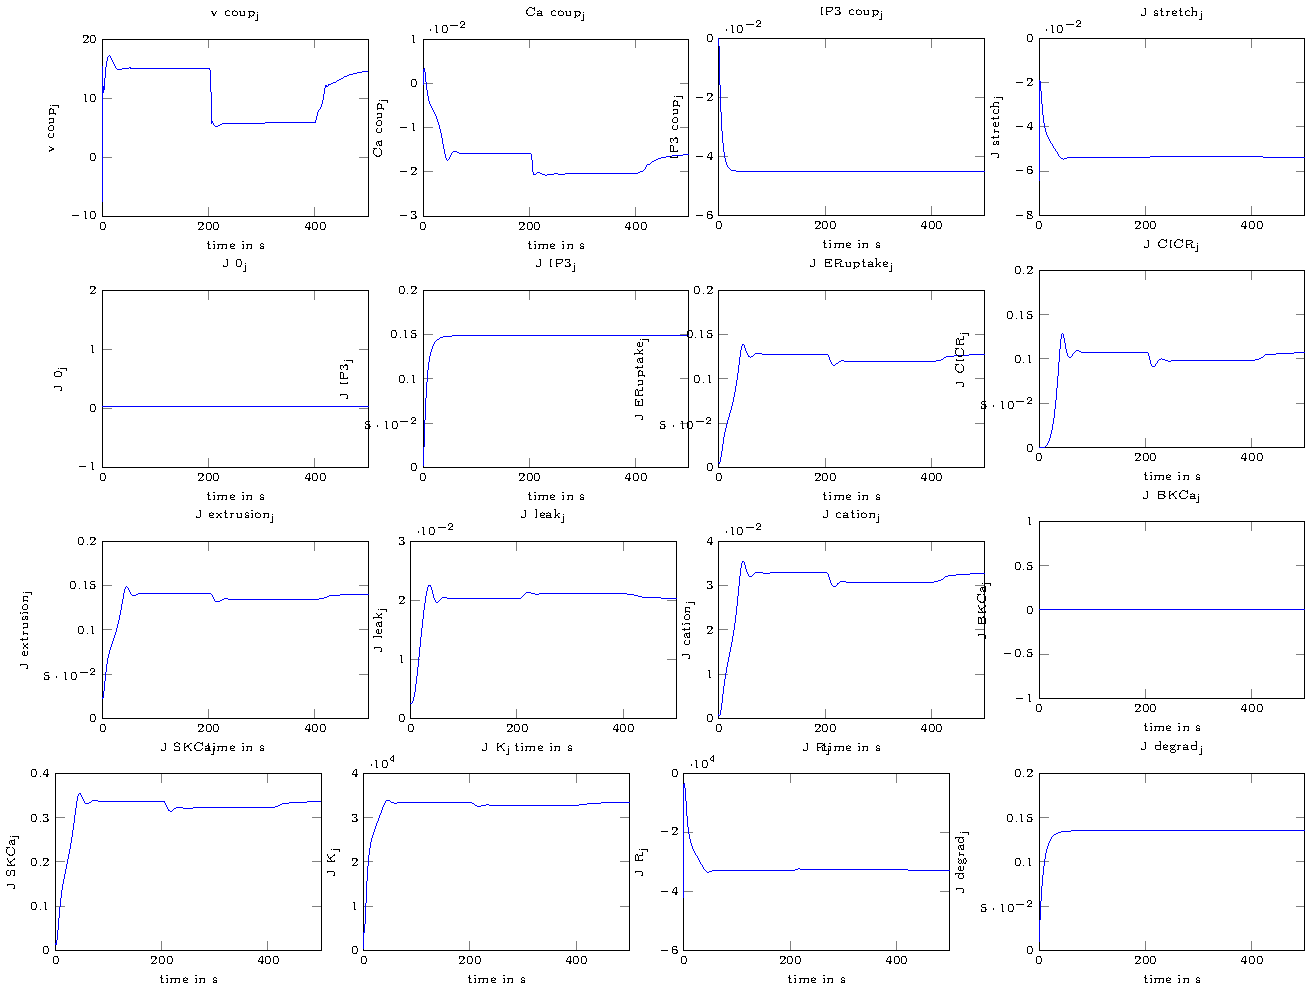
\includegraphics{figures/3_EC_fluxes.pdf}
			\caption{The EC fluxes}
			\label{fig:3ECF}
		\end{figure}
		\begin{figure}[h!]
			\centering
			\tiny  
			\setlength\figureheight{3.5 cm} 
			\setlength\figurewidth{6 cm}
			%% % This file was created by matlab2tikz v0.3.3.
% Copyright (c) 2008--2013, Nico Schlömer <nico.schloemer@gmail.com>
% All rights reserved.
% 
% The latest updates can be retrieved from
%   http://www.mathworks.com/matlabcentral/fileexchange/22022-matlab2tikz
% where you can also make suggestions and rate matlab2tikz.
% 
% 
% 
\begin{tikzpicture}

\begin{axis}[%
width=\figurewidth,
height=\figureheight,
scale only axis,
xmin=0,
xmax=500,
xlabel={time in s},
ymin=0,
ymax=1.5,
ylabel={$\text{s}_\text{i}\text{ in uM}$},
name=plot5,
title={$\text{SR [Ca}^{\text{2+}}\text{]}$}
]
\addplot [
color=blue,
solid,
forget plot
]
table[row sep=crcr]{
0 0.1\\
0.0011996 0.100020997699054\\
0.0023992 0.100041961177898\\
0.0035988 0.10006288981726\\
0.0085566 0.100149044088696\\
0.013514 0.10023462383532\\
0.018472 0.100319626866413\\
0.02343 0.100404057808573\\
0.033542 0.100574528622955\\
0.043655 0.100742719175691\\
0.053767 0.100908703011126\\
0.063879 0.101072554170175\\
0.073991 0.101234345784314\\
0.084819 0.101405385082737\\
0.095647 0.101574235925304\\
0.10647 0.101740988175198\\
0.1173 0.101905732181338\\
0.12813 0.102068558948308\\
0.14659 0.102341979822108\\
0.16505 0.10261056324248\\
0.18351 0.102874791992761\\
0.20197 0.10313517484965\\
0.22042 0.103392257945488\\
0.26398 0.103989616872483\\
0.30753 0.104582622824281\\
0.35108 0.105186358717979\\
0.37397 0.105514484202143\\
0.38969 0.105746575759548\\
0.4054 0.10598554194326\\
0.42111 0.106232117337024\\
0.43393 0.106439436485609\\
0.44676 0.106652284924968\\
0.45959 0.10687075288845\\
0.47242 0.107094900260472\\
0.48525 0.107324765297774\\
0.50035 0.107602639785962\\
0.51544 0.107888484791715\\
0.53054 0.108182306675517\\
0.54564 0.108484102098485\\
0.56073 0.108793861055774\\
0.57728 0.109142383651724\\
0.59382 0.109500423163078\\
0.61036 0.109867948966047\\
0.6269 0.110244926337347\\
0.64344 0.110631316826533\\
0.65998 0.11102707826095\\
0.69992 0.11202087944021\\
0.73986 0.113068287190176\\
0.77979 0.114168457971156\\
0.81973 0.115320435199594\\
0.85967 0.116523165833724\\
0.99616 0.120994152320654\\
1.1327 0.125992476390627\\
1.2692 0.131465299944458\\
1.4056 0.137356784435982\\
1.6062 0.14666357149725\\
1.8067 0.156599882913339\\
2.0072 0.167022405868248\\
2.2078 0.177814227589489\\
2.4083 0.188883200384409\\
2.8551 0.214228932448612\\
3.302 0.240063381680571\\
3.7488 0.266081766193055\\
4.1956 0.292145070158122\\
4.6425 0.318181566510773\\
5.3586 0.359742148813713\\
6.0748 0.400977282485852\\
6.791 0.441821032290392\\
7.5072 0.482225967778634\\
8.2234 0.522128433867584\\
9.2234 0.57684546963969\\
10.223 0.630194122319504\\
11.223 0.681951457653064\\
12.223 0.731883457347009\\
12.523 0.746470131232831\\
12.823 0.760860575249073\\
13.123 0.775046488970435\\
13.423 0.789020779863114\\
13.513 0.793170817270811\\
13.603 0.797301094147079\\
13.693 0.801411422129136\\
13.783 0.805501606360865\\
13.873 0.809571459536716\\
13.929 0.812068626052836\\
13.948 0.812918969282607\\
13.967 0.813768399581837\\
13.986 0.814616915257468\\
14.004 0.815464514630145\\
14.023 0.816311196041737\\
14.079 0.818773439409118\\
14.134 0.821227831649713\\
14.189 0.823674332246704\\
14.244 0.82611290090032\\
14.299 0.828543497533565\\
14.354 0.830966082303569\\
14.409 0.833380615616884\\
14.465 0.835787058143548\\
14.52 0.838197239642154\\
14.575 0.840599171121362\\
14.631 0.842992813474943\\
14.686 0.845378127849747\\
14.742 0.847755075639525\\
14.811 0.850721228900044\\
14.88 0.853674114119141\\
14.95 0.856613657118515\\
15.019 0.859539784485867\\
15.089 0.862452423637164\\
15.202 0.867162538465412\\
15.315 0.871836451845133\\
15.428 0.876473867643761\\
15.541 0.881074497686647\\
15.654 0.885638061882995\\
15.804 0.891650984801781\\
15.954 0.897597216216471\\
16.104 0.903476164041142\\
16.255 0.909287263492628\\
16.405 0.915029977117016\\
16.675 0.925192766611185\\
16.946 0.935129632083997\\
17.216 0.944838142131943\\
17.487 0.95431620776945\\
17.757 0.963562090089366\\
18.061 0.973652396005169\\
18.364 0.983447598328439\\
18.667 0.992946862655207\\
18.971 1.00214991503849\\
19.274 1.01105705317193\\
19.375 1.0139506906247\\
19.476 1.01681181303769\\
19.576 1.01964047109681\\
19.677 1.02243671892027\\
19.778 1.02520061905405\\
19.938 1.0295136111226\\
20.097 1.0337458963482\\
20.257 1.03789782387912\\
20.416 1.04196978015062\\
20.576 1.04596218686454\\
20.994 1.05602968733444\\
21.411 1.06556611057806\\
21.828 1.07458161422093\\
22.056 1.07927695337527\\
22.119 1.08056434451023\\
22.183 1.08184012225602\\
22.247 1.08310431401393\\
22.31 1.08435695705601\\
22.432 1.08672266102286\\
22.554 1.08904653138188\\
22.676 1.09132890814331\\
22.798 1.09357013534623\\
22.92 1.09577055813771\\
23.367 1.10350672339908\\
23.684 1.10866141841438\\
24 1.11355814537809\\
24.242 1.11713085025811\\
24.484 1.12055965257984\\
24.726 1.12384751287221\\
24.968 1.12699737936314\\
25.298 1.13107478202899\\
25.628 1.13490840466211\\
25.958 1.13850593667777\\
26.288 1.14187493552193\\
26.618 1.14502280798073\\
27.087 1.14913293906949\\
27.556 1.15283137051956\\
28.025 1.15613850166819\\
28.494 1.15907431365015\\
28.964 1.16165833883551\\
29.615 1.16470382824985\\
30.266 1.16715810768224\\
30.917 1.16906706768966\\
31.569 1.17047580526152\\
32.372 1.17158424212512\\
33.175 1.17207113804658\\
33.979 1.17201055879798\\
34.782 1.17146914127868\\
35.586 1.1705062029579\\
36.23 1.16946597751645\\
36.875 1.16821570401188\\
37.52 1.16677737069745\\
38.164 1.16517278252991\\
38.969 1.162967272223\\
39.774 1.16057883291926\\
40.579 1.15805581507264\\
41.384 1.15545199751116\\
42.189 1.15282800590739\\
43.189 1.14964649883472\\
44.189 1.14668813180803\\
45.189 1.1440993583316\\
46.189 1.14200623031162\\
47.189 1.14049224345722\\
48.189 1.13958209115571\\
49.189 1.13923811855797\\
50.189 1.13936627422315\\
51.189 1.13985010870011\\
52.189 1.1405690419597\\
53.189 1.14140952079917\\
54.189 1.14227714424103\\
55.189 1.14310054056863\\
56.189 1.14383126771854\\
57.189 1.14444267576195\\
58.189 1.14492002605048\\
59.189 1.1452601438032\\
60.189 1.14546882995817\\
61.189 1.14555710540711\\
62.189 1.14553914782941\\
63.189 1.14543103060976\\
64.189 1.14525042146286\\
65.189 1.14501597178163\\
66.189 1.14474590929722\\
67.189 1.14445747349753\\
68.189 1.14416577910028\\
69.189 1.1438865958819\\
70.189 1.14363412274776\\
71.189 1.14341653647269\\
72.189 1.14323366296032\\
73.189 1.14309172824772\\
74.189 1.14299308755916\\
75.189 1.14293714309011\\
76.189 1.14292580182136\\
77.189 1.14294567237217\\
78.189 1.14298944303281\\
79.189 1.14305135546346\\
80.189 1.14312599029412\\
81.189 1.14321012042192\\
82.189 1.14329691806612\\
83.189 1.14338296709281\\
84.189 1.14346560238409\\
85.189 1.14354192583921\\
86.189 1.14360921888463\\
87.189 1.14366821274108\\
88.189 1.14371892854538\\
89.189 1.14376099734391\\
90.189 1.14379472313629\\
91.189 1.14382037404349\\
92.189 1.1438389865391\\
93.189 1.14385146257085\\
94.189 1.14385942840143\\
95.189 1.14386405998913\\
96.189 1.1438671160796\\
97.189 1.14386958067441\\
98.189 1.14387295460152\\
99.189 1.14387771005421\\
100.19 1.14388490798619\\
101.19 1.14389441417009\\
102.19 1.14390688015305\\
103.19 1.14392164236925\\
104.19 1.14393892579171\\
105.19 1.14395867417976\\
106.19 1.14398003420392\\
107.19 1.14400250214235\\
108.19 1.14402551295621\\
109.19 1.14404876675662\\
110.19 1.14407181392256\\
111.19 1.14409452071423\\
112.19 1.1441165461064\\
113.19 1.14413789482707\\
114.19 1.14415830283291\\
115.19 1.14417789651181\\
116.19 1.14419645960483\\
117.19 1.14421422336432\\
118.19 1.14423099195392\\
119.19 1.14424708662541\\
120.19 1.14426230216245\\
121.19 1.14427703537373\\
122.19 1.14429104005673\\
123.19 1.1443046864223\\
124.19 1.14431814122636\\
125.19 1.14433131345575\\
126.19 1.14434420704318\\
127.19 1.1443568326917\\
128.19 1.14436926358074\\
129.19 1.14438150748666\\
130.19 1.14439363239791\\
131.19 1.14440562563074\\
132.19 1.14441753902706\\
133.19 1.14442932948852\\
134.19 1.14444103675914\\
135.19 1.14445259309986\\
136.19 1.1444640366234\\
137.19 1.1444752838\\
138.19 1.14448638299433\\
139.19 1.14449724130999\\
140.19 1.14450792598854\\
141.19 1.14451833669498\\
142.19 1.14452856439338\\
143.19 1.14453849903436\\
144.19 1.14454825768144\\
145.19 1.14455771559038\\
146.19 1.14456701753918\\
147.19 1.14457601776159\\
148.19 1.14458489091643\\
149.19 1.14459346329161\\
150.19 1.14460194286837\\
151.19 1.14461012065202\\
152.19 1.14461824298156\\
153.19 1.14462605767379\\
154.19 1.14463385620837\\
155.19 1.1446413344371\\
156.19 1.14464883765413\\
157.19 1.1446559997414\\
158.19 1.14466309903201\\
159.19 1.14467027004338\\
160.19 1.14467732767084\\
161.19 1.14468421274501\\
162.19 1.14469087688255\\
163.19 1.14469735774071\\
164.19 1.14470363189278\\
165.19 1.1447097583976\\
166.19 1.14471571509372\\
167.19 1.14472156596488\\
168.19 1.14472727332701\\
169.19 1.1447329021911\\
170.19 1.14473839673022\\
171.19 1.1447438259748\\
172.19 1.1447491174807\\
173.19 1.14475435048673\\
174.19 1.14475943725835\\
175.19 1.14476447267823\\
176.19 1.14476935291492\\
177.19 1.14477419250948\\
178.19 1.14477886847836\\
179.19 1.14478351835786\\
180.19 1.14478799552645\\
181.19 1.14479246420551\\
182.19 1.14479674888228\\
183.19 1.14480104521162\\
184.19 1.14480514294329\\
185.19 1.14480927524751\\
186.19 1.14481319047278\\
187.19 1.14481716677166\\
188.19 1.14482090321447\\
189.19 1.14482473184396\\
190.19 1.14482829296518\\
191.19 1.14483185746186\\
192.19 1.14483555257688\\
193.19 1.14483919393167\\
194.19 1.1448427248322\\
195.19 1.14484609235914\\
196.19 1.14484930416922\\
196.81 1.14485123069272\\
197.25 1.14485258424302\\
197.57 1.14485356215526\\
197.82 1.14485432516899\\
198.03 1.14485494063556\\
198.24 1.14485555165725\\
198.38 1.14485596653351\\
198.52 1.144856379158\\
198.63 1.14485670377287\\
198.74 1.14485702681849\\
198.83 1.14485729053029\\
198.92 1.1448575530411\\
199.01 1.14485781426041\\
199.17 1.14485824559778\\
199.32 1.14485867279218\\
199.47 1.1448590949376\\
199.62 1.14485951095091\\
199.84 1.14486010493768\\
200.07 1.1448606758515\\
200.29 1.14486121238742\\
200.51 1.14486171532483\\
200.69 1.14486213785538\\
200.87 1.14486268359625\\
201.05 1.14486358586528\\
201.23 1.14486525882894\\
201.42 1.14486837399173\\
201.6 1.14487409416568\\
201.79 1.14488402415674\\
201.97 1.14490058401331\\
202.15 1.14492727050631\\
202.34 1.14496905691138\\
202.63 1.14508449056394\\
202.92 1.14529812760442\\
203.21 1.14567400692043\\
203.5 1.14630532863198\\
203.79 1.14731687571343\\
204.09 1.14892648841984\\
204.39 1.15126239769\\
204.69 1.1544112059264\\
204.94 1.15757538460341\\
205.19 1.16112119519857\\
205.44 1.16485707793952\\
205.68 1.16856875442978\\
205.85 1.17102955432575\\
206.02 1.17338576012695\\
206.19 1.17562090401321\\
206.36 1.17772668254605\\
206.6 1.18049632297256\\
206.84 1.18300729356224\\
207.08 1.18527601051536\\
207.32 1.18732377845919\\
207.65 1.18983299073207\\
207.99 1.19201935634983\\
208.32 1.19393611756834\\
208.65 1.19562816118798\\
208.99 1.19713105800261\\
209.66 1.19972358318907\\
210.18 1.20139462849741\\
210.7 1.20285679300182\\
211.22 1.20415315721004\\
211.74 1.20531829310308\\
212.26 1.20637953015523\\
212.9 1.20757816076002\\
213.54 1.20868076122668\\
214.18 1.20971089301502\\
214.82 1.21068697620463\\
215.46 1.21162383648095\\
216.16 1.21262083399931\\
216.87 1.21359784127767\\
217.57 1.21456478098821\\
218.27 1.21552919957268\\
218.98 1.21649661119142\\
219.98 1.21788556078261\\
220.98 1.21929800668481\\
221.98 1.22073882672362\\
222.98 1.2222095869423\\
223.98 1.22370915862873\\
224.98 1.22523294620808\\
225.98 1.2267759779165\\
226.98 1.22833306610597\\
227.98 1.22989745483134\\
228.98 1.23146377718608\\
229.98 1.2330272364015\\
230.98 1.23458218270251\\
231.98 1.23612266634204\\
232.98 1.23764262865722\\
233.98 1.23913815002601\\
234.98 1.24060561522885\\
235.98 1.2420419817695\\
236.98 1.24344576966315\\
237.98 1.24481537508477\\
238.98 1.24614107448549\\
239.98 1.24743091836087\\
240.98 1.24868843226521\\
241.98 1.24991226984688\\
242.98 1.25110423429245\\
243.98 1.25226577942341\\
244.98 1.25339848944152\\
245.98 1.25450382865134\\
246.98 1.25558325798739\\
247.98 1.25663809860671\\
248.98 1.25766960019318\\
249.98 1.25867885874418\\
250.98 1.2596668579795\\
251.98 1.26063442542245\\
252.98 1.26158226629872\\
253.98 1.26251094873943\\
254.98 1.26342093579101\\
255.98 1.26431258725249\\
256.98 1.26518618816963\\
257.98 1.26604195772299\\
258.98 1.26688007291383\\
259.98 1.26770067914802\\
260.98 1.26850390861156\\
261.98 1.26928988941558\\
262.98 1.27005875834676\\
263.98 1.2708106668332\\
264.98 1.27154578824221\\
265.98 1.27226432020669\\
266.98 1.2729664872827\\
267.98 1.27365254011278\\
268.98 1.27432275465547\\
269.98 1.27497742913373\\
270.98 1.27561688114589\\
271.98 1.2762414434627\\
272.98 1.27685146021171\\
273.98 1.27744728247567\\
274.98 1.27802926449281\\
275.98 1.27859775976996\\
276.98 1.27915311793119\\
277.98 1.27969568177275\\
278.98 1.28022578508582\\
279.98 1.28074375081162\\
280.98 1.28124988990585\\
281.98 1.28174450053982\\
282.98 1.28222786788834\\
283.98 1.28270026418223\\
284.98 1.28316194919244\\
285.98 1.28361317087049\\
286.98 1.28405416626169\\
287.98 1.28448516246183\\
288.98 1.28490637770595\\
289.98 1.28531802240485\\
290.98 1.28572030020489\\
291.98 1.28611340892844\\
292.98 1.28649754146575\\
293.98 1.28687288651249\\
294.98 1.28723962922226\\
295.98 1.28759795169867\\
296.98 1.287948033395\\
297.98 1.28829005136958\\
298.98 1.28862418046172\\
299.98 1.28895059335313\\
300.98 1.28926946057444\\
301.98 1.28958095043245\\
302.98 1.28988522891052\\
303.98 1.29018245952385\\
304.98 1.29047280317369\\
305.98 1.29075641798479\\
306.98 1.29103345916157\\
307.98 1.29130407884802\\
308.98 1.29156842601839\\
309.98 1.2918266463838\\
310.98 1.29207888233434\\
311.98 1.29232527290164\\
312.98 1.29256595375564\\
313.98 1.29280105722081\\
314.98 1.2930307123209\\
315.98 1.29325504483853\\
316.98 1.29347417739557\\
317.98 1.29368822954191\\
318.98 1.29389731785696\\
319.98 1.2941015560531\\
320.98 1.2943010550845\\
321.98 1.29449592325255\\
322.98 1.29468626631103\\
323.98 1.29487218756416\\
324.98 1.29505378796071\\
325.98 1.29523116617901\\
326.98 1.29540441870625\\
327.98 1.29557363990829\\
328.98 1.2957389220936\\
329.98 1.29590035556848\\
330.98 1.2960580286872\\
331.98 1.29621202789515\\
332.98 1.29636243776824\\
333.98 1.2965093410472\\
334.98 1.29665281866976\\
335.98 1.29679294979962\\
336.98 1.29692981185461\\
337.98 1.2970634805333\\
338.98 1.2971940298419\\
339.98 1.29732153212063\\
340.98 1.29744605807116\\
341.98 1.29756767678415\\
342.98 1.29768645576812\\
343.98 1.29780246097875\\
344.98 1.29791575684934\\
345.98 1.29802640632172\\
346.98 1.29813447087809\\
347.98 1.29824001057301\\
348.98 1.29834308406588\\
349.98 1.29844374865329\\
350.98 1.29854206030152\\
351.98 1.29863807367845\\
352.98 1.29873184218524\\
353.98 1.2988234179873\\
354.98 1.29891285204465\\
355.98 1.29900019414131\\
356.98 1.29908549291407\\
357.98 1.29916879588013\\
358.98 1.29925014946395\\
359.98 1.29932959902319\\
360.98 1.29940718887366\\
361.98 1.29948296231353\\
362.98 1.29955696164663\\
363.98 1.29962922820502\\
364.98 1.29969980237091\\
365.98 1.29976872359779\\
366.98 1.2998360304311\\
367.98 1.2999017605283\\
368.98 1.29996595067847\\
369.98 1.3000286368214\\
370.98 1.30008985406639\\
371.98 1.30014963671055\\
372.98 1.30020801825683\\
373.98 1.3002650314317\\
374.98 1.30032070820249\\
375.98 1.30037507979445\\
376.98 1.30042817670751\\
377.98 1.30048002873274\\
378.98 1.3005306649685\\
379.98 1.3005801138363\\
380.98 1.30062840309634\\
381.98 1.3006755598628\\
382.98 1.30072161061872\\
383.98 1.30076658123068\\
384.98 1.30081049696307\\
385.98 1.30085338249209\\
386.98 1.30089526191945\\
387.98 1.30093615878566\\
388.98 1.30097609608315\\
389.98 1.30101509626898\\
390.98 1.30105318127722\\
391.98 1.30109037253116\\
392.98 1.30112669095522\\
393.98 1.30116215698717\\
394.98 1.30119679059447\\
395.98 1.3012306113228\\
396.98 1.30126363858388\\
397.98 1.30129587435669\\
398.44 1.30131049845496\\
398.8 1.30132187116355\\
399.07 1.30133051741313\\
399.35 1.30133909796273\\
399.55 1.30134535148122\\
399.76 1.30135156733166\\
399.96 1.30135774756076\\
400.26 1.30136697767057\\
400.34 1.301369851227\\
400.43 1.3013728547265\\
400.52 1.3013760530589\\
400.61 1.30137952476316\\
400.92 1.30139618755118\\
401.24 1.30142195854678\\
401.56 1.30146093021066\\
401.87 1.30151702517297\\
402.11 1.30157308283698\\
402.35 1.30164241376229\\
402.59 1.30172613882813\\
402.83 1.301825175017\\
403.14 1.30197732681802\\
403.45 1.30215754836332\\
403.77 1.30236661729355\\
404.08 1.30260486098853\\
404.39 1.30287223814377\\
404.93 1.30340774913331\\
405.47 1.30402765904616\\
406.02 1.30472717325448\\
406.56 1.30550043446306\\
407.1 1.30634106304326\\
408.1 1.3080414709675\\
408.77 1.30926267446058\\
409.43 1.31053863519465\\
410.1 1.31185501982409\\
410.61 1.31289044343752\\
411.12 1.31394295907093\\
411.63 1.31501596601629\\
412.15 1.31611574233747\\
412.66 1.31724997988463\\
413.31 1.31874314072915\\
413.95 1.3203151618134\\
414.6 1.32197605743121\\
415.25 1.32373347869359\\
415.9 1.32559255478727\\
416.77 1.32827175021917\\
417.65 1.33112747104879\\
418.52 1.33411622713991\\
419.4 1.33714388742268\\
420.28 1.34006404247126\\
421.2 1.34286269785022\\
422.12 1.34527107047956\\
423.04 1.34728572826353\\
423.96 1.34897471160248\\
424.89 1.35034408673076\\
425.81 1.35129885547322\\
426.73 1.35175244560273\\
427.68 1.35167305336524\\
428.64 1.35108979328041\\
429.59 1.35007776299273\\
430.55 1.3486649253207\\
431.5 1.34682776276738\\
432.5 1.34442353051537\\
433.5 1.34155891636426\\
434.5 1.33831416728025\\
435.5 1.33476106136746\\
436.5 1.33094140186568\\
437.5 1.32687011283588\\
438.5 1.32257713026389\\
439.5 1.31811917764565\\
440.5 1.31356372591239\\
441.5 1.30895633896148\\
442.5 1.30432600292119\\
443.5 1.29971643450487\\
444.5 1.29516080770211\\
445.5 1.29068105047026\\
446.5 1.28629286716763\\
447.5 1.28200837466334\\
448.5 1.27781460380174\\
449.5 1.27372914206628\\
450.5 1.26976593598147\\
451.5 1.26593244704481\\
452.5 1.26223148093902\\
453.5 1.25866279585636\\
454.5 1.25522415550299\\
455.5 1.25191206557839\\
456.5 1.24872230170938\\
457.5 1.24565025996812\\
458.5 1.24269118034151\\
459.5 1.23984028491107\\
460.5 1.23709286245442\\
461.5 1.2344443227757\\
462.5 1.23189023164231\\
463.5 1.22942633296594\\
464.5 1.2270485621898\\
465.5 1.22475305277482\\
466.5 1.22253613776896\\
467.5 1.22039434764852\\
468.5 1.21832440533128\\
469.5 1.21632321923706\\
470.5 1.21438787485875\\
471.5 1.21251562535749\\
472.5 1.21070388157097\\
473.5 1.20895020170521\\
474.5 1.20725228102462\\
475.5 1.20560794171821\\
476.5 1.204015123121\\
477.5 1.20247187243712\\
478.5 1.20097633603832\\
479.5 1.19952675143575\\
480.5 1.19812143995714\\
481.5 1.1967588001545\\
482.5 1.19543730195412\\
483.5 1.19415548151164\\
484.5 1.19291193674753\\
485.5 1.19170532349714\\
486.5 1.19053435220619\\
487.5 1.18939778510329\\
488.5 1.18829443375752\\
489.5 1.18722315695576\\
490.5 1.18618285881959\\
491.5 1.18517248709727\\
492.5 1.18419103158159\\
493.5 1.18323752259688\\
494.5 1.18231102953116\\
495.5 1.18141065937931\\
496.5 1.18053555528313\\
497.5 1.17968489506433\\
498.5 1.17885788973901\\
499.5 1.17805378203075\\
500 1.17766137592547\\
};
\end{axis}

\begin{axis}[%
width=\figurewidth,
height=\figureheight,
scale only axis,
xmin=0,
xmax=500,
xlabel={time in s},
ymin=0,
ymax=0.8,
ylabel={$\text{Ca}_\text{j}\text{ in uM}$},
name=plot2,
at=(plot5.above north west),
anchor=below south west,
title={$\text{EC [Ca}^{\text{2+}}\text{]}$}
]
\addplot [
color=blue,
solid,
forget plot
]
table[row sep=crcr]{
0 0.1\\
0.0011996 0.0999317558517299\\
0.0023992 0.0998658905116772\\
0.0035988 0.0998023444108983\\
0.0085566 0.0995599291315511\\
0.013514 0.0993485763097409\\
0.018472 0.0991634585137531\\
0.02343 0.0989999628744725\\
0.033542 0.0987189944219344\\
0.043655 0.0984871563348061\\
0.053767 0.0982871861163715\\
0.063879 0.0981086285209446\\
0.073991 0.0979449582507401\\
0.084819 0.0977812898667575\\
0.095647 0.0976259315687315\\
0.10647 0.0974764503020281\\
0.1173 0.0973313290210947\\
0.12813 0.0971896217140476\\
0.14659 0.0969544392860456\\
0.16505 0.0967257004779483\\
0.18351 0.0965026293859647\\
0.20197 0.0962850066543483\\
0.22042 0.0960727801457476\\
0.26398 0.0955936409885522\\
0.30753 0.095145933310985\\
0.35108 0.0947324107662572\\
0.37397 0.0945299891083472\\
0.38969 0.0943975151231675\\
0.4054 0.0942704656321336\\
0.42111 0.0941489077237188\\
0.43393 0.0940537232727711\\
0.44676 0.0939621546064645\\
0.45959 0.0938741417358264\\
0.47242 0.0937896163933149\\
0.48525 0.0937085096823074\\
0.50035 0.0936173511574225\\
0.51544 0.0935307494445015\\
0.53054 0.0934486311217051\\
0.54564 0.0933709391159642\\
0.56073 0.0932976298610276\\
0.57728 0.0932222979877418\\
0.59382 0.0931521522102015\\
0.61036 0.0930871635896022\\
0.6269 0.09302730593271\\
0.64344 0.0929725543703145\\
0.65998 0.0929228847611854\\
0.69992 0.0928237677768262\\
0.73986 0.0927537874461377\\
0.77979 0.0927125893819221\\
0.81973 0.0926998075701114\\
0.85967 0.0927150674479478\\
0.99616 0.0929715211023911\\
1.1327 0.0935352433619547\\
1.2692 0.0943908258240911\\
1.4056 0.0955220350805506\\
1.6062 0.0976512147529939\\
1.8067 0.100289141469834\\
2.0072 0.103383161240371\\
2.2078 0.106882315959942\\
2.4083 0.110737674589308\\
2.8551 0.120377817007867\\
3.302 0.131076552858118\\
3.7488 0.142414678344564\\
4.1956 0.154046826934358\\
4.6425 0.165701382698157\\
5.3586 0.183966689141971\\
6.0748 0.201234802217388\\
6.791 0.217230918806046\\
7.5072 0.231881575752058\\
8.2234 0.245219495273618\\
9.2234 0.261819582567922\\
10.223 0.276330867117439\\
11.223 0.289096091641359\\
12.223 0.300442143754414\\
12.523 0.303615093463052\\
12.823 0.306692411541751\\
13.123 0.309680349643393\\
13.423 0.312585351530224\\
13.513 0.313441635033633\\
13.603 0.314291180182563\\
13.693 0.315134136670064\\
13.783 0.315970654164703\\
13.873 0.316800881984444\\
13.929 0.317309304226595\\
13.948 0.317482270667623\\
13.967 0.317654970945909\\
13.986 0.317827406396828\\
14.004 0.317999578354666\\
14.023 0.318171488147378\\
14.079 0.318671004043726\\
14.134 0.319168336990851\\
14.189 0.319663519173078\\
14.244 0.320156582439542\\
14.299 0.320647558315871\\
14.354 0.321136478014524\\
14.409 0.321623372439866\\
14.465 0.3221082721905\\
14.52 0.322593596767593\\
14.575 0.323076967875716\\
14.631 0.323558415639616\\
14.686 0.324037969871373\\
14.742 0.324515660071143\\
14.811 0.32511156030959\\
14.88 0.325704637104279\\
14.95 0.326294946459231\\
15.019 0.326882543636957\\
15.089 0.327467483190483\\
15.202 0.328413691184797\\
15.315 0.329353233897192\\
15.428 0.330286335230796\\
15.541 0.331213214486615\\
15.654 0.332134086596015\\
15.804 0.333350158754038\\
15.954 0.334556457318452\\
16.104 0.335753454504833\\
16.255 0.336941609651406\\
16.405 0.338121369801507\\
16.675 0.340225117451153\\
16.946 0.342305512617517\\
17.216 0.344364891635147\\
17.487 0.346405478874525\\
17.757 0.348429398244285\\
18.061 0.350681682017797\\
18.364 0.352918295937926\\
18.667 0.355141852796464\\
18.971 0.357354852746787\\
19.274 0.359559688755629\\
19.375 0.360290746904991\\
19.476 0.361021238398374\\
19.576 0.361751244350729\\
19.677 0.362480845379134\\
19.778 0.363210120707082\\
19.938 0.364365085123384\\
20.097 0.365519732351945\\
20.257 0.36667436234372\\
20.416 0.367829269760508\\
20.576 0.368984744396668\\
20.994 0.37201132269986\\
21.411 0.375048683820433\\
21.828 0.378101470417034\\
22.056 0.379772347360628\\
22.119 0.380241195040741\\
22.183 0.380710600944838\\
22.247 0.381180572825624\\
22.31 0.381651122743103\\
22.432 0.382553494852014\\
22.554 0.383458145567297\\
22.676 0.384365186687\\
22.798 0.385274729021743\\
22.92 0.386186881429935\\
23.367 0.389560248672548\\
23.684 0.391972524762387\\
24 0.394407592324847\\
24.242 0.396285334776476\\
24.484 0.398178328404303\\
24.726 0.400087393939231\\
24.968 0.402013344342853\\
25.298 0.404667898529959\\
25.628 0.407357366902812\\
25.958 0.410083883065693\\
26.288 0.412849559043658\\
26.618 0.415656489044234\\
27.087 0.419723459616263\\
27.556 0.423884192878684\\
28.025 0.428144829792195\\
28.494 0.432511560741269\\
28.964 0.436990606381648\\
29.615 0.443406921611305\\
30.266 0.450067866236001\\
30.917 0.45698892201493\\
31.569 0.464185053692257\\
32.372 0.473459951045336\\
33.175 0.483193085801922\\
33.979 0.493395192788265\\
34.782 0.504060857405512\\
35.586 0.515161714579315\\
36.23 0.524343973503811\\
36.875 0.533715730371456\\
37.52 0.543208192544378\\
38.164 0.552729735451441\\
38.969 0.564490250565959\\
39.774 0.575852495151066\\
40.579 0.586493545526785\\
41.384 0.596073505875308\\
42.189 0.604267756377133\\
43.189 0.612160613249423\\
44.189 0.617261725348163\\
45.189 0.619555671917183\\
46.189 0.619291508296858\\
47.189 0.616918346942347\\
48.189 0.612990941648383\\
49.189 0.608079022319395\\
50.189 0.602736885203962\\
51.189 0.597365479720492\\
52.189 0.592277631516004\\
53.189 0.587704922638491\\
54.189 0.583800268341943\\
55.189 0.580646449869139\\
56.189 0.578268691684869\\
57.189 0.576652535485653\\
58.189 0.575748829023812\\
59.189 0.575482075827411\\
60.189 0.57576000957021\\
61.189 0.576481199392335\\
62.189 0.577534647103505\\
63.189 0.578821699756294\\
64.189 0.580248156548726\\
65.189 0.581725683577585\\
66.189 0.583175034784983\\
67.189 0.584536412822794\\
68.189 0.585744711882651\\
69.189 0.586714198927721\\
70.189 0.587459823772176\\
71.189 0.587988849976963\\
72.189 0.588343987419051\\
73.189 0.588522026387472\\
74.189 0.588532768892989\\
75.189 0.58839719172247\\
76.189 0.588139682513499\\
77.189 0.587812708871426\\
78.189 0.587448729399549\\
79.189 0.58707343520602\\
80.189 0.586707796920346\\
81.189 0.586356741883845\\
82.189 0.586044270600179\\
83.189 0.585776800005055\\
84.189 0.585560374051007\\
85.189 0.58539611519061\\
86.189 0.585294817877013\\
87.189 0.585233556610677\\
88.189 0.585215855809376\\
89.189 0.585235421852825\\
90.189 0.585286603896271\\
91.189 0.585359740540315\\
92.189 0.58544888531322\\
93.189 0.585544716345126\\
94.189 0.58564308459662\\
95.189 0.585736191362991\\
96.189 0.585822522746196\\
97.189 0.585896116117368\\
98.189 0.585958266639659\\
99.189 0.586004583408369\\
100.19 0.586038905186632\\
101.19 0.586057778871214\\
102.19 0.586067095158856\\
103.19 0.586063538667031\\
104.19 0.586051242248556\\
105.19 0.586033753969335\\
106.19 0.586012218729222\\
107.19 0.585989042382631\\
108.19 0.585964877093744\\
109.19 0.58594193347479\\
110.19 0.585920249129906\\
111.19 0.585901691005316\\
112.19 0.585885558501223\\
113.19 0.585873412492788\\
114.19 0.585863849844122\\
115.19 0.585858286951037\\
116.19 0.585854720350277\\
117.19 0.585854631500954\\
118.19 0.585855523137954\\
119.19 0.58585915381021\\
120.19 0.585862605466992\\
121.19 0.585868103469499\\
122.19 0.585872328048564\\
123.19 0.585876747803556\\
124.19 0.585880919547113\\
125.19 0.585884639922248\\
126.19 0.585887941788976\\
127.19 0.585890470358656\\
128.19 0.585892405166425\\
129.19 0.585893473536976\\
130.19 0.585894004733141\\
131.19 0.585893750099885\\
132.19 0.585893148808607\\
133.19 0.585891923652073\\
134.19 0.585890598344259\\
135.19 0.585888823928197\\
136.19 0.585887195883058\\
137.19 0.585885258226213\\
138.19 0.585883678349777\\
139.19 0.585881865409828\\
140.19 0.585880571703211\\
141.19 0.585879049252274\\
142.19 0.58587815968338\\
143.19 0.58587697798475\\
144.19 0.585876508829931\\
145.19 0.585875628889483\\
146.19 0.585875526848426\\
147.19 0.585874854774703\\
148.19 0.585875032247195\\
149.19 0.585874452380886\\
150.19 0.585874818161786\\
151.19 0.585874218936476\\
152.19 0.585874700052683\\
153.19 0.585873989944388\\
154.19 0.585874543507432\\
155.19 0.585873657195808\\
156.19 0.585874273452074\\
157.19 0.58587317011898\\
158.19 0.585872503490654\\
159.19 0.585871792253881\\
160.19 0.585871130057165\\
161.19 0.585870757965503\\
162.19 0.585870372569096\\
163.19 0.585870221541492\\
164.19 0.585869966935746\\
165.19 0.585869927996187\\
166.19 0.585869716569918\\
167.19 0.58586972507111\\
168.19 0.585869498674124\\
169.19 0.585869514204649\\
170.19 0.585869235596542\\
171.19 0.585869239107055\\
172.19 0.585868889900433\\
173.19 0.585868880995772\\
174.19 0.585868457323217\\
175.19 0.585868449135349\\
176.19 0.585867955571518\\
177.19 0.585867968928893\\
178.19 0.585867412562448\\
179.19 0.585867471096364\\
180.19 0.585866856942085\\
181.19 0.585866983881396\\
182.19 0.585866311973296\\
183.19 0.58586652867447\\
184.19 0.585865792648237\\
185.19 0.585866118547814\\
186.19 0.585865305300505\\
187.19 0.585865758870187\\
188.19 0.585864848851856\\
189.19 0.585865449158797\\
190.19 0.585864416899185\\
191.19 0.585863862399307\\
192.19 0.585863294074755\\
193.19 0.585862804553253\\
194.19 0.585862622564383\\
195.19 0.585862580460815\\
196.19 0.585862608172265\\
196.81 0.585862644715805\\
197.25 0.585862678103352\\
197.57 0.585862705526451\\
197.82 0.58586272859981\\
198.03 0.585862748151738\\
198.24 0.585862768342417\\
198.38 0.585862782402757\\
198.52 0.585862796688128\\
198.63 0.585862808109495\\
198.74 0.585862819644627\\
198.83 0.585862829175746\\
198.92 0.5858628387747\\
199.01 0.585862848439511\\
199.17 0.585862864625013\\
199.32 0.585862880993468\\
199.47 0.585862897578427\\
199.62 0.585862914431557\\
199.84 0.585862939702526\\
200.07 0.585862966219323\\
200.29 0.585862994842027\\
200.51 0.585863025351714\\
200.69 0.585863048563365\\
200.87 0.585863060454323\\
201.05 0.585863041255672\\
201.23 0.585862955881386\\
201.42 0.585862747179711\\
201.6 0.585862316562195\\
201.79 0.585861524909231\\
201.97 0.585860162701893\\
202.15 0.585857925223696\\
202.34 0.585854375729094\\
202.63 0.585844432199943\\
202.92 0.585825757950198\\
203.21 0.585792333144017\\
203.5 0.585734859415109\\
203.79 0.585639592984418\\
204.09 0.585480040854789\\
204.39 0.585230561657235\\
204.69 0.584857481452085\\
204.94 0.584434483108247\\
205.19 0.583890497196931\\
205.44 0.583219945006015\\
205.68 0.582428990863183\\
205.85 0.581823891521477\\
206.02 0.581172502188433\\
206.19 0.580479794829311\\
206.36 0.57975060818452\\
206.6 0.578660238412195\\
206.84 0.577517885148092\\
207.08 0.576334971219547\\
207.32 0.575121973200818\\
207.65 0.573410285299334\\
207.99 0.571680096235325\\
208.32 0.569950667165984\\
208.65 0.568238001591523\\
208.99 0.566555412766146\\
209.66 0.563269797370463\\
210.18 0.560914186928963\\
210.7 0.558725198475236\\
211.22 0.55671912693643\\
211.74 0.55490707946158\\
212.26 0.553295680038307\\
212.9 0.551584543461022\\
213.54 0.550182384174603\\
214.18 0.549081735689412\\
214.82 0.548270223488163\\
215.46 0.547731826463275\\
216.16 0.547432895351185\\
216.87 0.547412649578647\\
217.57 0.547641439391953\\
218.27 0.548088204631715\\
218.98 0.548721237610935\\
219.98 0.549879478258606\\
220.98 0.55125976318013\\
221.98 0.552775410275622\\
222.98 0.554345630855051\\
223.98 0.555896847639747\\
224.98 0.557360557577547\\
225.98 0.558688989392686\\
226.98 0.559845751227276\\
227.98 0.560802691973485\\
228.98 0.561545296065125\\
229.98 0.562069722444846\\
230.98 0.562382440953537\\
231.98 0.562499667222337\\
232.98 0.562445329907449\\
233.98 0.562248876054044\\
234.98 0.561945570518049\\
235.98 0.561565554270189\\
236.98 0.561138113836849\\
237.98 0.560690813103978\\
238.98 0.560256853194645\\
239.98 0.559856589595368\\
240.98 0.559503842256998\\
241.98 0.559205338404117\\
242.98 0.558965177500251\\
243.98 0.558784405778895\\
244.98 0.558661370268766\\
245.98 0.558592246168076\\
246.98 0.558571561429527\\
247.98 0.558592708785474\\
248.98 0.558648406780816\\
249.98 0.558731116062465\\
250.98 0.558833391717075\\
251.98 0.558948178194916\\
252.98 0.559069038112911\\
253.98 0.559190321920182\\
254.98 0.559307276668457\\
255.98 0.559416101987153\\
256.98 0.559513956389166\\
257.98 0.55959892308736\\
258.98 0.559669941355997\\
259.98 0.559726712823514\\
260.98 0.559769589665396\\
261.98 0.559799453119148\\
262.98 0.559817588585993\\
263.98 0.55982556381455\\
264.98 0.559825114676265\\
265.98 0.559818042626137\\
266.98 0.559806126217424\\
267.98 0.559791048423748\\
268.98 0.559774340170909\\
269.98 0.559757339954316\\
270.98 0.559741168492704\\
271.98 0.559726717063823\\
272.98 0.55971464764332\\
273.98 0.559705402902056\\
274.98 0.559699223915576\\
275.98 0.559696173565808\\
276.98 0.559696163638894\\
277.98 0.559698983871905\\
278.98 0.5597043313572\\
279.98 0.559711839016456\\
280.98 0.559721102068337\\
281.98 0.559731701716501\\
282.98 0.559743225496781\\
283.98 0.559755283986191\\
284.98 0.559767523752543\\
285.98 0.559779636626097\\
286.98 0.559791365495733\\
287.98 0.559802506965383\\
288.98 0.559812911267595\\
289.98 0.559822479898185\\
290.98 0.559831161442975\\
291.98 0.559838946080029\\
292.98 0.559845859206499\\
293.98 0.559851954613007\\
294.98 0.559857307568741\\
295.98 0.559862008132734\\
296.98 0.559866154937165\\
297.98 0.559869849634511\\
298.98 0.559873192133645\\
299.98 0.559876276701083\\
300.98 0.559879188948498\\
301.98 0.559882003690772\\
302.98 0.559884783619774\\
303.98 0.559887578717077\\
304.98 0.559890426306289\\
305.98 0.559893351638072\\
306.98 0.55989636889283\\
307.98 0.559899482490064\\
308.98 0.559902688596167\\
309.98 0.559905976734247\\
310.98 0.559909331409107\\
311.98 0.559912733676222\\
312.98 0.55991616259602\\
313.98 0.55991959653103\\
314.98 0.559923014255768\\
315.98 0.559926395863595\\
316.98 0.559929723464849\\
317.98 0.559932981681578\\
318.98 0.559936157950976\\
319.98 0.559939242656758\\
320.98 0.559942229111027\\
321.98 0.559945113412632\\
322.98 0.559947894208257\\
323.98 0.559950572382976\\
324.98 0.559953150704976\\
325.98 0.559955633447551\\
326.98 0.559958026008142\\
327.98 0.559960334541448\\
328.98 0.559962565619848\\
329.98 0.559964725931316\\
330.98 0.559966822021426\\
331.98 0.55996886008334\\
332.98 0.559970845796695\\
333.98 0.559972784214308\\
334.98 0.559974679693529\\
335.98 0.559976535867878\\
336.98 0.559978355653425\\
337.98 0.559980141283969\\
338.98 0.559981894368662\\
339.98 0.559983615965983\\
340.98 0.559985306668112\\
341.98 0.559986966690455\\
342.98 0.559988595961584\\
343.98 0.559990194209741\\
344.98 0.55999176104273\\
345.98 0.559993296018952\\
346.98 0.55999479870797\\
347.98 0.559996268739804\\
348.98 0.559997705842711\\
349.98 0.55999910986977\\
350.98 0.560000480814995\\
351.98 0.560001818820063\\
352.98 0.560003124172912\\
353.98 0.560004397299662\\
354.98 0.560005638751308\\
355.98 0.560006849186649\\
356.98 0.560008029352821\\
357.98 0.560009180064674\\
358.98 0.560010302184085\\
359.98 0.560011396600127\\
360.98 0.560012464210787\\
361.98 0.560013505906805\\
362.98 0.56001452255796\\
363.98 0.560015515002007\\
364.98 0.560016484036308\\
365.98 0.560017430412084\\
366.98 0.560018354831098\\
367.98 0.56001925794453\\
368.98 0.560020140353737\\
369.98 0.560021002612552\\
370.98 0.560021845230793\\
371.98 0.56002266867863\\
372.98 0.560023473391496\\
373.98 0.560024259775243\\
374.98 0.560025028211305\\
375.98 0.560025779061635\\
376.98 0.560026512673274\\
377.98 0.560027229382401\\
378.98 0.560027929517811\\
379.98 0.560028613403751\\
380.98 0.560029281362129\\
381.98 0.560029933714101\\
382.98 0.560030570781073\\
383.98 0.560031192885207\\
384.98 0.560031800349464\\
385.98 0.560032393497291\\
386.98 0.56003297265203\\
387.98 0.560033538136111\\
388.98 0.560034090270125\\
389.98 0.560034629371836\\
390.98 0.560035155755191\\
391.98 0.560035669729394\\
392.98 0.560036171598177\\
393.98 0.560036661660001\\
394.98 0.560037140214423\\
395.98 0.560037607613135\\
396.98 0.560038064639392\\
397.98 0.560038515755938\\
398.44 0.560038719248024\\
398.8 0.560038874981717\\
399.07 0.560038991095261\\
399.35 0.560039103400206\\
399.55 0.560039183716509\\
399.76 0.560039262241277\\
399.96 0.560039339425162\\
400.26 0.560039538924175\\
400.34 0.560039630996589\\
400.43 0.560039760189663\\
400.52 0.560039943010428\\
400.61 0.560040198616623\\
400.92 0.560042177548234\\
401.24 0.560046388631\\
401.56 0.560053781733505\\
401.87 0.560065278213983\\
402.11 0.560077231109869\\
402.35 0.560092369834953\\
402.59 0.560110974527598\\
402.83 0.56013327930257\\
403.14 0.560167960976458\\
403.45 0.560209480401226\\
403.77 0.560258054659564\\
404.08 0.560313782611757\\
404.39 0.560376659342054\\
404.93 0.560503235781912\\
405.47 0.560650276785835\\
406.02 0.560816223939749\\
406.56 0.560999058035726\\
407.1 0.561196444777676\\
408.1 0.561588762379888\\
408.77 0.561862968045093\\
409.43 0.562140691057956\\
410.1 0.562415927345173\\
410.61 0.562623270034854\\
411.12 0.562825337639079\\
411.63 0.563022556658793\\
412.15 0.56321647017857\\
412.66 0.563409291009912\\
413.31 0.56365522146055\\
413.95 0.56390868552481\\
414.6 0.564175294988946\\
415.25 0.564461106815025\\
415.9 0.564772789413072\\
416.77 0.565249346494421\\
417.65 0.565808040601408\\
418.52 0.566471484000672\\
419.4 0.56725938211508\\
420.28 0.568177031670777\\
421.2 0.569258843626506\\
422.12 0.570396769916956\\
423.04 0.571507470183522\\
423.96 0.572526192309842\\
424.89 0.573433744904924\\
425.81 0.574249068921919\\
426.73 0.574995990796785\\
427.68 0.575697543114671\\
428.64 0.576311551670992\\
429.59 0.576826454642583\\
430.55 0.577245915325638\\
431.5 0.577586475275305\\
432.5 0.577878947277718\\
433.5 0.578120121799865\\
434.5 0.578318786386833\\
435.5 0.578483322395265\\
436.5 0.57862508381417\\
437.5 0.578756633999778\\
438.5 0.578887696455164\\
439.5 0.579023148855817\\
440.5 0.579164440736257\\
441.5 0.579312711654962\\
442.5 0.579468755427374\\
443.5 0.579633709305133\\
444.5 0.579803894687853\\
445.5 0.579977058201202\\
446.5 0.580151160046514\\
447.5 0.580324233149857\\
448.5 0.580495317565971\\
449.5 0.580662742539049\\
450.5 0.580824828358691\\
451.5 0.580980163173022\\
452.5 0.581127731826389\\
453.5 0.581266951532807\\
454.5 0.581397645842557\\
455.5 0.581519984286\\
456.5 0.581634410243939\\
457.5 0.581741568991813\\
458.5 0.581842240426193\\
459.5 0.581937278439838\\
460.5 0.582027557673828\\
461.5 0.582113928301818\\
462.5 0.582197179495468\\
463.5 0.582278011839872\\
464.5 0.582357018654728\\
465.5 0.582434675753599\\
466.5 0.58251133880346\\
467.5 0.58258724721785\\
468.5 0.582662533330992\\
469.5 0.58273723553933\\
470.5 0.582811314108839\\
471.5 0.58288466840932\\
472.5 0.582957154470981\\
473.5 0.5830286019124\\
474.5 0.583098829472679\\
475.5 0.583167658576891\\
476.5 0.583234924550364\\
477.5 0.583300485282426\\
478.5 0.583364227300241\\
479.5 0.583426069351452\\
480.5 0.583485963708078\\
481.5 0.583543895484355\\
482.5 0.583599880318702\\
483.5 0.583653960797661\\
484.5 0.583706202004127\\
485.5 0.58375668655844\\
486.5 0.583805509487043\\
487.5 0.583852773211102\\
488.5 0.583898582894551\\
489.5 0.58394304233438\\
490.5 0.583986250520475\\
491.5 0.584028298936082\\
492.5 0.584069269622183\\
493.5 0.584109233985228\\
494.5 0.584148252292719\\
495.5 0.584186373775547\\
496.5 0.584223637236148\\
497.5 0.584260072053247\\
498.5 0.584295699469657\\
499.5 0.584330534053475\\
500 0.584347602817767\\
};
\end{axis}

\begin{axis}[%
width=\figurewidth,
height=\figureheight,
scale only axis,
xmin=0,
xmax=500,
xlabel={time in s},
ymin=0.05,
ymax=0.3,
ylabel={$\text{Ca}_\text{i}\text{ in uM}$},
name=plot1,
at=(plot2.left of south west),
anchor=right of south east,
title={$\text{SMC [Ca}^{\text{2+}}\text{]}$}
]
\addplot [
color=blue,
solid,
forget plot
]
table[row sep=crcr]{
0 0.1\\
0.0011996 0.0999273303630155\\
0.0023992 0.099854827688845\\
0.0035988 0.0997824978613758\\
0.0085566 0.0994853319464782\\
0.013514 0.0991912301894956\\
0.018472 0.0989003602341548\\
0.02343 0.0986128455037873\\
0.033542 0.0980371427488988\\
0.043655 0.0974763621321031\\
0.053767 0.0969309457484875\\
0.063879 0.0964012275784077\\
0.073991 0.0958874976108007\\
0.084819 0.0953554633105539\\
0.095647 0.0948424281575875\\
0.10647 0.0943487710145348\\
0.1173 0.0938749221612575\\
0.12813 0.0934213742785212\\
0.14659 0.0926967277973565\\
0.16505 0.09203627601956\\
0.18351 0.0914445454473639\\
0.20197 0.090927514766051\\
0.22042 0.0904930703961802\\
0.26398 0.0898729407668077\\
0.30753 0.0900306554413631\\
0.35108 0.0913622125223461\\
0.37397 0.09265150753555\\
0.38969 0.0937654883903477\\
0.4054 0.0950153140401243\\
0.42111 0.0963493709112061\\
0.43393 0.097470637077011\\
0.44676 0.0986039155835637\\
0.45959 0.0997399585335789\\
0.47242 0.100873278898548\\
0.48525 0.102000563954398\\
0.50035 0.103316829524329\\
0.51544 0.104619777601361\\
0.53054 0.10590815595626\\
0.54564 0.107181278899913\\
0.56073 0.108438784518695\\
0.57728 0.109798465563091\\
0.59382 0.111139129139543\\
0.61036 0.112460845736258\\
0.6269 0.113763734090951\\
0.64344 0.115047919410123\\
0.65998 0.116313518441741\\
0.69992 0.119293067114409\\
0.73986 0.122166340679509\\
0.77979 0.124934741266217\\
0.81973 0.127599841716548\\
0.85967 0.130163491440482\\
0.99616 0.138200254639176\\
1.1327 0.145170021011389\\
1.2692 0.151170932177262\\
1.4056 0.156308329444031\\
1.6062 0.162496919298532\\
1.8067 0.167350044056928\\
2.0072 0.171151966720965\\
2.2078 0.174141505893584\\
2.4083 0.176509521826615\\
2.8551 0.18020549560408\\
3.302 0.182655926752287\\
3.7488 0.184500853094179\\
4.1956 0.186039022517288\\
4.6425 0.187418557601377\\
5.3586 0.189498706731981\\
6.0748 0.191598244346243\\
6.791 0.193774758776037\\
7.5072 0.196025876383118\\
8.2234 0.198334700451135\\
9.2234 0.201632077372733\\
10.223 0.205023458245931\\
11.223 0.208553629082284\\
12.223 0.212184821142884\\
12.523 0.213273978814699\\
12.823 0.214351089140804\\
13.123 0.215425138239315\\
13.423 0.216502975778666\\
13.513 0.216827445758333\\
13.603 0.217151789693776\\
13.693 0.217475858773817\\
13.783 0.217799686109416\\
13.873 0.21812331331705\\
13.929 0.218322594706672\\
13.948 0.218390576794393\\
13.967 0.218458546819329\\
13.986 0.218526504592031\\
14.004 0.218594450014333\\
14.023 0.218662382871928\\
14.079 0.218860285764748\\
14.134 0.219058071709411\\
14.189 0.219255732847084\\
14.244 0.219453261268008\\
14.299 0.219650649254394\\
14.354 0.219847889473412\\
14.409 0.220044975060185\\
14.465 0.220241899373696\\
14.52 0.220439630344668\\
14.575 0.220637183201148\\
14.631 0.220834548413465\\
14.686 0.221031715184179\\
14.742 0.221228671859333\\
14.811 0.221475119167403\\
14.88 0.221721194605083\\
14.95 0.221966876074308\\
15.019 0.222212143516246\\
15.089 0.222456979443395\\
15.202 0.222854391130946\\
15.315 0.223250569613813\\
15.428 0.223645472604891\\
15.541 0.22403906374195\\
15.654 0.224431307342701\\
15.804 0.224950947088819\\
15.954 0.225468032831643\\
16.104 0.225982451936861\\
16.255 0.226494080088603\\
16.405 0.227002783209674\\
16.675 0.227910609921601\\
16.946 0.228807684311817\\
17.216 0.229693231375403\\
17.487 0.230566578126021\\
17.757 0.231427157198882\\
18.061 0.232376397190898\\
18.364 0.233308334803563\\
18.667 0.234222418359417\\
18.971 0.235118194998119\\
19.274 0.235995336076759\\
19.375 0.236282560470836\\
19.476 0.236567703239225\\
19.576 0.23685076183099\\
19.677 0.237131734175286\\
19.778 0.237410619854278\\
19.938 0.237848210646734\\
20.097 0.238280580745361\\
20.257 0.238707752101513\\
20.416 0.239129755862329\\
20.576 0.239546631624514\\
20.994 0.240612937008864\\
21.411 0.241645647717887\\
21.828 0.242646073405856\\
22.056 0.243177881221181\\
22.119 0.243325123965955\\
22.183 0.243471679976441\\
22.247 0.243617554163701\\
22.31 0.243762752236616\\
22.432 0.244038820358891\\
22.554 0.24431247680262\\
22.676 0.244583765708141\\
22.798 0.244852730712394\\
22.92 0.245119414871319\\
23.367 0.246079920081714\\
23.684 0.246742537327815\\
24 0.247391765482036\\
24.242 0.247879388672496\\
24.484 0.24835991400661\\
24.726 0.24883364149863\\
24.968 0.249300851875735\\
25.298 0.249927813135538\\
25.628 0.250543741982397\\
25.958 0.251149236732258\\
26.288 0.251744843587926\\
26.618 0.252331050821141\\
27.087 0.253149343630639\\
27.556 0.253950567204913\\
28.025 0.25473562178758\\
28.494 0.255505238456025\\
28.964 0.256260011521004\\
29.615 0.257284294690458\\
30.266 0.258282397517821\\
30.917 0.259255195279702\\
31.569 0.260203479230173\\
32.372 0.261340665061012\\
33.175 0.262443370767537\\
33.979 0.263513983307995\\
34.782 0.264555566956002\\
35.586 0.265571300261498\\
36.23 0.266369336308182\\
36.875 0.267153091887212\\
37.52 0.267922241258192\\
38.164 0.268675059253284\\
38.969 0.26958692134274\\
39.774 0.270457098862812\\
40.579 0.271268295803542\\
41.384 0.271997325486358\\
42.189 0.272617367790078\\
43.189 0.273190922860042\\
44.189 0.273502481975864\\
45.189 0.273525790872083\\
46.189 0.273268923409576\\
47.189 0.272779116982352\\
48.189 0.272136093066634\\
49.189 0.271434140337433\\
50.189 0.270759103698012\\
51.189 0.270173228703679\\
52.189 0.269710588627933\\
53.189 0.269381318550833\\
54.189 0.269176955860571\\
55.189 0.269078664037914\\
56.189 0.269064203130116\\
57.189 0.269112133771374\\
58.189 0.269204524077185\\
59.189 0.269327536142064\\
60.189 0.269469768614727\\
61.189 0.269622402272461\\
62.189 0.269779322218154\\
63.189 0.269932663908802\\
64.189 0.270076055486128\\
65.189 0.27020457468748\\
66.189 0.270314772881484\\
67.189 0.270405426698473\\
68.189 0.270474005890537\\
69.189 0.270518719649754\\
70.189 0.270540170101225\\
71.189 0.270541178761954\\
72.189 0.270524830818272\\
73.189 0.270494303763238\\
74.189 0.270452593448994\\
75.189 0.270403213410438\\
76.189 0.270354557063255\\
77.189 0.270306606445791\\
78.189 0.270261048134401\\
79.189 0.270219194339357\\
80.189 0.270182163807865\\
81.189 0.270148657685084\\
82.189 0.270121983362578\\
83.189 0.270101652566097\\
84.189 0.270087758775781\\
85.189 0.270079208177536\\
86.189 0.270074298585756\\
87.189 0.27007150807789\\
88.189 0.270071487939388\\
89.189 0.270073464938267\\
90.189 0.270077531112359\\
91.189 0.270082452974442\\
92.189 0.270088181133855\\
93.189 0.270093264041298\\
94.189 0.270097890887713\\
95.189 0.2701007069497\\
96.189 0.270102366871742\\
97.189 0.270101685375936\\
98.189 0.27009982889703\\
99.189 0.270095684002822\\
100.19 0.270090854549751\\
101.19 0.27008412376395\\
102.19 0.270077438788737\\
103.19 0.270069304479196\\
104.19 0.270061089456211\\
105.19 0.270053063363882\\
106.19 0.270045279813152\\
107.19 0.270038100214326\\
108.19 0.270031283982214\\
109.19 0.270025172127568\\
110.19 0.27001938614769\\
111.19 0.270014290767437\\
112.19 0.270009420912272\\
113.19 0.270005201391159\\
114.19 0.270001073295694\\
115.19 0.269997546769451\\
116.19 0.269993959205325\\
117.19 0.26999092780525\\
118.19 0.269987672673978\\
119.19 0.269984945536383\\
120.19 0.269981832413445\\
121.19 0.269979251072877\\
122.19 0.269976131096177\\
123.19 0.269973158228553\\
124.19 0.269970192475597\\
125.19 0.269967247789166\\
126.19 0.26996436685746\\
127.19 0.269961445811375\\
128.19 0.269958563863315\\
129.19 0.269955619278512\\
130.19 0.269952718001527\\
131.19 0.26994975686805\\
132.19 0.269946873387499\\
133.19 0.269943946895226\\
134.19 0.26994114051117\\
135.19 0.269938305105669\\
136.19 0.269935627871087\\
137.19 0.269932922201794\\
138.19 0.269930403528051\\
139.19 0.269927841664651\\
140.19 0.269925488198717\\
141.19 0.269923064006791\\
142.19 0.269920867077851\\
143.19 0.269918562778702\\
144.19 0.269916507020379\\
145.19 0.269914300784428\\
146.19 0.269912370541746\\
147.19 0.269910241227351\\
148.19 0.269908424071261\\
149.19 0.269906353320708\\
150.19 0.269904641410783\\
151.19 0.269902614054944\\
152.19 0.26990100431613\\
153.19 0.269899007920188\\
154.19 0.269897501690184\\
155.19 0.269895525701561\\
156.19 0.269894128165177\\
157.19 0.269892162858948\\
158.19 0.269890433907553\\
159.19 0.269888760520939\\
160.19 0.269887161034291\\
161.19 0.269885697361728\\
162.19 0.269884248799177\\
163.19 0.269882899010692\\
164.19 0.269881518793222\\
165.19 0.269880217126402\\
166.19 0.269878857449264\\
167.19 0.269877583384214\\
168.19 0.269876239012073\\
169.19 0.269875000435303\\
170.19 0.269873682815388\\
171.19 0.269872495433649\\
172.19 0.269871215299396\\
173.19 0.269870089897681\\
174.19 0.269868850437668\\
175.19 0.269867790723652\\
176.19 0.269866588460904\\
177.19 0.26986559408333\\
178.19 0.269864422511631\\
179.19 0.269863492682334\\
180.19 0.269862345026261\\
181.19 0.269861480526046\\
182.19 0.269860350601777\\
183.19 0.269859554083476\\
184.19 0.269858435821772\\
185.19 0.269857711306963\\
186.19 0.269856597888623\\
187.19 0.269855950301443\\
188.19 0.269854833521685\\
189.19 0.269854268635535\\
190.19 0.26985313863256\\
191.19 0.269852222459652\\
192.19 0.269851352460126\\
193.19 0.269850540891393\\
194.19 0.269849847043072\\
195.19 0.269849213481286\\
196.19 0.269848589397593\\
196.81 0.269848204121076\\
197.25 0.269847928097221\\
197.57 0.269847726608275\\
197.82 0.269847568877376\\
198.03 0.26984744191049\\
198.24 0.269847316945961\\
198.38 0.269847233010564\\
198.52 0.269847150853751\\
198.63 0.269847087360815\\
198.74 0.269847025615689\\
198.83 0.269846976437773\\
198.92 0.269846928940215\\
199.01 0.269846883432799\\
199.17 0.26984681243081\\
199.32 0.269846749095344\\
199.47 0.269846696009456\\
199.62 0.269846656368475\\
199.84 0.269846630694656\\
200.07 0.26984667792246\\
200.29 0.26984682746293\\
200.51 0.269846882749389\\
200.69 0.269846379625881\\
200.87 0.269844469226456\\
201.05 0.269839818656556\\
201.23 0.269830520978625\\
201.42 0.269813828753433\\
201.6 0.269785181189708\\
201.79 0.269738873830677\\
201.97 0.269666625547525\\
202.15 0.269556897727923\\
202.34 0.269393718327403\\
202.63 0.2689704455004\\
202.92 0.268234081608663\\
203.21 0.267005248629307\\
203.5 0.265030610311634\\
203.79 0.261974769192562\\
204.09 0.257232879356706\\
204.39 0.250459470401199\\
204.69 0.241434003506634\\
204.94 0.232466699615662\\
205.19 0.22264532882655\\
205.44 0.212728245707161\\
205.68 0.203468446547266\\
205.85 0.19768614814247\\
206.02 0.192415304321435\\
206.19 0.187642314397958\\
206.36 0.183338640556531\\
206.6 0.17795001300562\\
206.84 0.173343204174652\\
207.08 0.169415360272986\\
207.32 0.166067366386913\\
207.65 0.162236974771004\\
207.99 0.159152650770788\\
208.32 0.156653596770323\\
208.65 0.154617759750904\\
208.99 0.152952171605323\\
209.66 0.15042689759599\\
210.18 0.149027040573389\\
210.7 0.147959424026424\\
211.22 0.147144199929401\\
211.74 0.146519381165389\\
212.26 0.146038688289912\\
212.9 0.14559839326182\\
213.54 0.14528913073067\\
214.18 0.145082662930757\\
214.82 0.144958727382777\\
215.46 0.144901957609719\\
216.16 0.144902441394249\\
216.87 0.144955428741661\\
217.57 0.145049837877627\\
218.27 0.145176663187318\\
218.98 0.145328827422537\\
219.98 0.145577597483626\\
220.98 0.145853331605181\\
221.98 0.146146286372854\\
222.98 0.146447175230709\\
223.98 0.146745279695989\\
224.98 0.147030046744441\\
225.98 0.147297000407451\\
226.98 0.147544338489351\\
227.98 0.147774170456791\\
228.98 0.147987282710192\\
229.98 0.148182267605921\\
230.98 0.148356182411837\\
231.98 0.148507278390333\\
232.98 0.148637626950199\\
233.98 0.148750291542026\\
234.98 0.148848654080707\\
235.98 0.148935218849245\\
236.98 0.149010835901509\\
237.98 0.149078397123805\\
238.98 0.149138406946008\\
239.98 0.149194168678102\\
240.98 0.149246795125532\\
241.98 0.149300210673264\\
242.98 0.149354526867231\\
243.98 0.14941032514278\\
244.98 0.149467697797026\\
245.98 0.149526826671137\\
246.98 0.149587593006288\\
247.98 0.149649914041884\\
248.98 0.14971351083862\\
249.98 0.1497781141322\\
250.98 0.14984333741986\\
251.98 0.149908814483895\\
252.98 0.149974134904717\\
253.98 0.150038933179018\\
254.98 0.1501028518055\\
255.98 0.150165593891551\\
256.98 0.150226898265579\\
257.98 0.150286568246159\\
258.98 0.150344453083747\\
259.98 0.150400461842435\\
260.98 0.150454548029748\\
261.98 0.15050671402439\\
262.98 0.150556997442024\\
263.98 0.150605470094477\\
264.98 0.150652226058634\\
265.98 0.150697378260204\\
266.98 0.150741048699157\\
267.98 0.150783364747363\\
268.98 0.150824451847728\\
269.98 0.150864430699667\\
270.98 0.150903412454779\\
271.98 0.15094149727674\\
272.98 0.150978771785386\\
273.98 0.1510153090031\\
274.98 0.151051167602596\\
275.98 0.151086392961428\\
276.98 0.151121017672167\\
277.98 0.151155063295603\\
278.98 0.151188541593978\\
279.98 0.151221456563973\\
280.98 0.151253805928921\\
281.98 0.151285583100456\\
282.98 0.151316778581911\\
283.98 0.151347381613533\\
284.98 0.151377381268229\\
285.98 0.151406767649661\\
286.98 0.151435532581642\\
287.98 0.151463670330508\\
288.98 0.151491177886607\\
289.98 0.151518055259763\\
290.98 0.151544305418364\\
291.98 0.151569934254669\\
292.98 0.151594950283064\\
293.98 0.151619364391449\\
294.98 0.151643189409227\\
295.98 0.151666439757203\\
296.98 0.151689130984524\\
297.98 0.151711279409799\\
298.98 0.151732901702462\\
299.98 0.151754014579878\\
300.98 0.151774634479971\\
301.98 0.151794777349713\\
302.98 0.15181445842836\\
303.98 0.151833692136913\\
304.98 0.151852491968961\\
305.98 0.1518708704714\\
306.98 0.151888839224654\\
307.98 0.151906408893125\\
308.98 0.151923589268726\\
309.98 0.151940389364753\\
310.98 0.151956817495165\\
311.98 0.151972881386438\\
312.98 0.151988588268169\\
313.98 0.152003944982095\\
314.98 0.152018958065546\\
315.98 0.152033633843288\\
316.98 0.152047978492309\\
317.98 0.152061998108934\\
318.98 0.152075698750011\\
319.98 0.152089086473702\\
320.98 0.152102167357435\\
321.98 0.152114947515183\\
322.98 0.152127433096191\\
323.98 0.152139630284212\\
324.98 0.152151545282878\\
325.98 0.152163184303397\\
326.98 0.15217455354282\\
327.98 0.152185659166417\\
328.98 0.15219650728436\\
329.98 0.152207103933858\\
330.98 0.152217455058404\\
331.98 0.152227566493166\\
332.98 0.152237443949328\\
333.98 0.152247093004614\\
334.98 0.152256519093726\\
335.98 0.15226572750445\\
336.98 0.152274723373979\\
337.98 0.152283511689998\\
338.98 0.152292097291845\\
339.98 0.152300484875357\\
340.98 0.152308678997392\\
341.98 0.15231668408297\\
342.98 0.152324504431631\\
343.98 0.152332144225453\\
344.98 0.152339607535906\\
345.98 0.152346898331601\\
346.98 0.152354020484639\\
347.98 0.152360977777312\\
348.98 0.152367773907323\\
349.98 0.152374412493042\\
350.98 0.152380897077349\\
351.98 0.152387231131363\\
352.98 0.152393418056944\\
353.98 0.152399461189074\\
354.98 0.152405363797242\\
355.98 0.152411129086787\\
356.98 0.152416760199503\\
357.98 0.152422260214304\\
358.98 0.152427632147397\\
359.98 0.152432878952616\\
360.98 0.152438003521464\\
361.98 0.152443008683401\\
362.98 0.152447897205978\\
363.98 0.152452671795267\\
364.98 0.15245733509623\\
365.98 0.152461889693393\\
366.98 0.152466338111498\\
367.98 0.152470682816442\\
368.98 0.152474926216209\\
369.98 0.152479070662028\\
370.98 0.152483118449534\\
371.98 0.152487071820079\\
372.98 0.152490932962032\\
373.98 0.152494704012173\\
374.98 0.152498387057043\\
375.98 0.152501984134348\\
376.98 0.152505497234285\\
377.98 0.152508928300896\\
378.98 0.152512279233317\\
379.98 0.152515551887039\\
380.98 0.152518748075053\\
381.98 0.152521869568994\\
382.98 0.152524918100172\\
383.98 0.152527895360596\\
384.98 0.1525308030039\\
385.98 0.152533642646251\\
386.98 0.152536415867187\\
387.98 0.152539124210433\\
388.98 0.152541769184663\\
389.98 0.152544352264255\\
390.98 0.152546874890046\\
391.98 0.152549338470349\\
392.98 0.152551744384018\\
393.98 0.152554093998753\\
394.98 0.152556388802092\\
395.98 0.152558631364836\\
396.98 0.152560832437665\\
397.98 0.152563078398962\\
398.44 0.152563982887856\\
398.8 0.152564594544299\\
399.07 0.152565008949113\\
399.35 0.152565373539871\\
399.55 0.152565647230732\\
399.76 0.152565935733005\\
399.96 0.152566261821319\\
400.26 0.152574378144841\\
400.34 0.152579524669168\\
400.43 0.152587478502924\\
400.52 0.152598992272676\\
400.61 0.152614649126199\\
400.92 0.152708825234996\\
401.24 0.152863165138422\\
401.56 0.153076231161783\\
401.87 0.153343367992725\\
402.11 0.153579275535112\\
402.35 0.153840110238491\\
402.59 0.154122936008808\\
402.83 0.154424810379949\\
403.14 0.154839741012218\\
403.45 0.155275994776651\\
403.77 0.155727970922913\\
404.08 0.156190831190522\\
404.39 0.156660426788516\\
404.93 0.157486646048333\\
405.47 0.158307228978427\\
406.02 0.159110737909375\\
406.56 0.159890117617389\\
407.1 0.160640371519266\\
408.1 0.161916800855014\\
408.77 0.162669837735986\\
409.43 0.163331367994902\\
410.1 0.163911982532481\\
410.61 0.164335543495819\\
411.12 0.164787892218202\\
411.63 0.165312261134494\\
412.15 0.165935942199667\\
412.66 0.166668677511783\\
413.31 0.167752716965255\\
413.95 0.169018529029688\\
414.6 0.170475517960773\\
415.25 0.172140969554522\\
415.9 0.17404097535342\\
416.77 0.17704746850195\\
417.65 0.180636664168589\\
418.52 0.184864745583305\\
419.4 0.189634560118478\\
420.28 0.194509033103715\\
421.2 0.198969736367958\\
422.12 0.202129659818947\\
423.04 0.204078218401504\\
423.96 0.205582021210698\\
424.89 0.207492539398147\\
425.81 0.210040050643896\\
426.73 0.212780231590257\\
427.68 0.215277765915767\\
428.64 0.217308538229454\\
429.59 0.219115148901435\\
430.55 0.220977263592342\\
431.5 0.222962293377556\\
432.5 0.225026763801689\\
433.5 0.226912926402762\\
434.5 0.228597373137347\\
435.5 0.230180472333423\\
436.5 0.231744676239337\\
437.5 0.233286653489031\\
438.5 0.234740626113643\\
439.5 0.236062426520488\\
440.5 0.237271364606238\\
441.5 0.23840825197342\\
442.5 0.239484420505672\\
443.5 0.240472992062204\\
444.5 0.241395995753137\\
445.5 0.242266122244568\\
446.5 0.243089809864607\\
447.5 0.243871012192916\\
448.5 0.244618941776161\\
449.5 0.245330852949966\\
450.5 0.246006408966654\\
451.5 0.246648962911635\\
452.5 0.247263040669395\\
453.5 0.247852735745591\\
454.5 0.248421227384888\\
455.5 0.248970775018194\\
456.5 0.249502978040634\\
457.5 0.250019018861672\\
458.5 0.250519818738295\\
459.5 0.251006140601547\\
460.5 0.251478639426296\\
461.5 0.251937889525599\\
462.5 0.252384403258328\\
463.5 0.252818641556444\\
464.5 0.253241023419749\\
465.5 0.253651933284962\\
466.5 0.25405172638071\\
467.5 0.254440733834153\\
468.5 0.254819266380146\\
469.5 0.25518761765229\\
470.5 0.255546067131512\\
471.5 0.255894882396026\\
472.5 0.256234321266619\\
473.5 0.256564633467758\\
474.5 0.25688606197159\\
475.5 0.257198844159349\\
476.5 0.257503212586575\\
477.5 0.257799395621878\\
478.5 0.258087617829396\\
479.5 0.258368100137606\\
480.5 0.258641059908704\\
481.5 0.258906710789478\\
482.5 0.259165262512612\\
483.5 0.25941692060408\\
484.5 0.259661886031479\\
485.5 0.259900354895015\\
486.5 0.260132518085159\\
487.5 0.26035856102851\\
488.5 0.260578663478466\\
489.5 0.260792999361371\\
490.5 0.261001736734822\\
491.5 0.261205037770344\\
492.5 0.261403058844797\\
493.5 0.261595950671703\\
494.5 0.261783858476284\\
495.5 0.261966922242938\\
496.5 0.262145276944832\\
497.5 0.262319052838146\\
498.5 0.26248837573235\\
499.5 0.262653367263097\\
500 0.262734003919981\\
};
\end{axis}

\begin{axis}[%
width=\figurewidth,
height=\figureheight,
scale only axis,
xmin=0,
xmax=500,
xlabel={time in s},
ymin=0,
ymax=1.5,
ylabel={$\text{I}_\text{j}\text{ in uM}$},
name=plot4,
at=(plot1.below south west),
anchor=above north west,
title={$\text{EC [IP}_{\text{3}}\text{]}$}
]
\addplot [
color=blue,
solid,
forget plot
]
table[row sep=crcr]{
0 0.1\\
0.0011996 0.100203901033589\\
0.0023992 0.100407765576334\\
0.0035988 0.100611592866175\\
0.0085566 0.101453614329679\\
0.013514 0.102295012468263\\
0.018472 0.103135777384012\\
0.02343 0.103975905934797\\
0.033542 0.105687523711705\\
0.043655 0.107396496017217\\
0.053767 0.109102828233509\\
0.063879 0.110806525932366\\
0.073991 0.112507593828774\\
0.084819 0.114326119438099\\
0.095647 0.116141640186189\\
0.10647 0.117954161524669\\
0.1173 0.119763688954977\\
0.12813 0.121570227968817\\
0.14659 0.124643035902727\\
0.16505 0.12770720193728\\
0.18351 0.130762752970605\\
0.20197 0.133809715809677\\
0.22042 0.136848117174011\\
0.26398 0.143983348738489\\
0.30753 0.151071413635686\\
0.35108 0.158112657116723\\
0.37397 0.161795170549638\\
0.38969 0.164314948438381\\
0.4054 0.166828717391146\\
0.42111 0.169336493295198\\
0.43393 0.171379734058096\\
0.44676 0.173418998286279\\
0.45959 0.175454294553754\\
0.47242 0.177485631415419\\
0.48525 0.179513017406888\\
0.50035 0.181893934038709\\
0.51544 0.184269404281125\\
0.53054 0.186639441942373\\
0.54564 0.189004060792332\\
0.56073 0.191363274563208\\
0.57728 0.193942033604602\\
0.59382 0.196514338148747\\
0.61036 0.199080206103347\\
0.6269 0.201639655322965\\
0.64344 0.204192703609667\\
0.65998 0.206739368712641\\
0.69992 0.212861512686241\\
0.73986 0.2189468015997\\
0.77979 0.224995481517035\\
0.81973 0.231007796655135\\
0.85967 0.236983989441799\\
0.99616 0.257141674932317\\
1.1327 0.276889850659778\\
1.2692 0.296237409557463\\
1.4056 0.315193359245286\\
1.6062 0.342348796570146\\
1.8067 0.368704328352056\\
2.0072 0.394286708921886\\
2.2078 0.419121421396186\\
2.4083 0.443232762898961\\
2.8551 0.4944739254366\\
3.302 0.542482179273193\\
3.7488 0.58748468272734\\
4.1956 0.629690515990191\\
4.6425 0.669292645376303\\
5.3586 0.727770261629675\\
6.0748 0.78067914221452\\
6.791 0.828611126489472\\
7.5072 0.872086329117395\\
8.2234 0.911564492829087\\
9.2234 0.960753397601023\\
10.223 1.00390601368559\\
11.223 1.04184743241618\\
12.223 1.07527336455274\\
12.523 1.08451602594479\\
12.823 1.09341870816502\\
13.123 1.10199575714068\\
13.423 1.11026122961547\\
13.513 1.11268214012248\\
13.603 1.11507649674322\\
13.693 1.11744461379298\\
13.783 1.1197868131681\\
13.873 1.12210341388532\\
13.929 1.12351802462999\\
13.948 1.12399856246438\\
13.967 1.12447799391799\\
13.986 1.12495632184341\\
14.004 1.12543354908752\\
14.023 1.12590967847851\\
14.079 1.12729103280574\\
14.134 1.12866315592226\\
14.189 1.13002611654997\\
14.244 1.13137998281266\\
14.299 1.13272482225669\\
14.354 1.13406070186678\\
14.409 1.13538768807234\\
14.465 1.13670584675042\\
14.52 1.13802171256936\\
14.575 1.13932879485166\\
14.631 1.1406271588001\\
14.686 1.14191686907315\\
14.742 1.14319798979033\\
14.811 1.14479104934366\\
14.88 1.14637084953734\\
14.95 1.14793751298823\\
15.019 1.14949116101024\\
15.089 1.15103191365286\\
15.202 1.15351160240093\\
15.315 1.15595797041566\\
15.428 1.15837151442061\\
15.541 1.16075272251818\\
15.654 1.16310207457158\\
15.804 1.16617881461991\\
15.954 1.16920110395735\\
16.104 1.17217000879442\\
16.255 1.17508657127095\\
16.405 1.1779518105552\\
16.675 1.18298296842895\\
16.946 1.18785669649483\\
17.216 1.19257842522666\\
17.487 1.19715336669833\\
17.757 1.20158653015875\\
18.061 1.20639514207184\\
18.364 1.21103804058998\\
18.667 1.21552147180352\\
18.971 1.21985142598765\\
19.274 1.22403364137234\\
19.375 1.22539127579311\\
19.476 1.22673340664828\\
19.576 1.22806022753614\\
19.677 1.22937193062718\\
19.778 1.23066870450815\\
19.938 1.23269315926542\\
20.097 1.23468132498549\\
20.257 1.23663390952563\\
20.416 1.23855160495163\\
20.576 1.24043508827316\\
20.994 1.24520450372934\\
21.411 1.24975601752183\\
21.828 1.25410002995022\\
22.056 1.25638209286874\\
22.119 1.2570105455824\\
22.183 1.25763460291555\\
22.247 1.25825428056454\\
22.31 1.25886960361711\\
22.432 1.26003539444125\\
22.554 1.26118556333605\\
22.676 1.26232033975874\\
22.798 1.2634399487453\\
22.92 1.26454460889806\\
23.367 1.26847660275374\\
23.684 1.27114457489641\\
24 1.27372153620446\\
24.242 1.27563184061352\\
24.484 1.27749239103638\\
24.726 1.27930457324213\\
24.968 1.28106972018241\\
25.298 1.28340283474737\\
25.628 1.28565398374825\\
25.958 1.28782630454882\\
26.288 1.28992276556368\\
26.618 1.29194617568515\\
27.087 1.29470311483257\\
27.556 1.29732508318342\\
28.025 1.29981904882899\\
28.494 1.3021915799973\\
28.964 1.30444887771253\\
29.615 1.30740377844015\\
30.266 1.31016273766475\\
30.917 1.31273891980301\\
31.569 1.3151448585599\\
32.372 1.31789446107571\\
33.175 1.32042220996297\\
33.979 1.32274724183595\\
34.782 1.32488663539586\\
35.586 1.32685566381558\\
36.23 1.32832229657319\\
36.875 1.32969528423091\\
37.52 1.33098041629471\\
38.164 1.33218329329449\\
38.969 1.33357714938055\\
39.774 1.33486043157688\\
40.579 1.33604237835855\\
41.384 1.33713128500818\\
42.189 1.33813460511209\\
43.189 1.33927200028639\\
44.189 1.34029963835501\\
45.189 1.34122826229692\\
46.189 1.34206751832268\\
47.189 1.34282608697642\\
48.189 1.34351179278567\\
49.189 1.34413169207363\\
50.189 1.34469268875153\\
51.189 1.34520015218665\\
52.189 1.34565903074552\\
53.189 1.34607393232332\\
54.189 1.34644907763\\
55.189 1.34678829344208\\
56.189 1.34709503694353\\
57.189 1.34737220431151\\
58.189 1.34762269719235\\
59.189 1.34784921553919\\
60.189 1.34805412894664\\
61.189 1.34823951198148\\
62.189 1.34840737568261\\
63.189 1.34855929808541\\
64.189 1.34869673947267\\
65.189 1.3488210621847\\
66.189 1.34893351586453\\
67.189 1.34903523509553\\
68.189 1.34912724626564\\
69.189 1.34920844554032\\
70.189 1.3492817633695\\
71.189 1.3493482360089\\
72.189 1.34940958046283\\
73.189 1.34946567688965\\
74.189 1.34951660427747\\
75.189 1.34956270415347\\
76.189 1.34960338055337\\
77.189 1.3496401091705\\
78.189 1.34967340993906\\
79.189 1.34970362468476\\
80.189 1.34973104295294\\
81.189 1.34975592419923\\
82.189 1.3497788916282\\
83.189 1.34979989524804\\
84.189 1.3498189639075\\
85.189 1.34983622551106\\
86.189 1.34985145699041\\
87.189 1.34986521065032\\
88.189 1.34987768104842\\
89.189 1.34988899609043\\
90.189 1.34989926412715\\
91.189 1.34990858225772\\
92.189 1.34991703840146\\
93.189 1.34992471231108\\
94.189 1.34993167635465\\
95.189 1.34993799620328\\
96.189 1.34994373145163\\
97.189 1.34994893618042\\
98.189 1.34995365946675\\
99.189 1.34995794584717\\
100.19 1.34996183573785\\
101.19 1.34996536581586\\
102.19 1.34996856936518\\
103.19 1.34997147659062\\
104.19 1.34997411490277\\
105.19 1.34997650917649\\
106.19 1.34997868198554\\
107.19 1.34998065381547\\
108.19 1.34998244325679\\
109.19 1.34998406718033\\
110.19 1.3499855408963\\
111.19 1.34998687829869\\
112.19 1.34998809199625\\
113.19 1.34998919343141\\
114.19 1.34999019298818\\
115.19 1.34999110009003\\
116.19 1.34999192328876\\
117.19 1.34999267034516\\
118.19 1.34999334830214\\
119.19 1.34999396355114\\
120.19 1.34999452189242\\
121.19 1.34999502858974\\
122.19 1.34999548841994\\
123.19 1.34999590571805\\
124.19 1.3499962844181\\
125.19 1.34999662809025\\
126.19 1.34999693997442\\
127.19 1.34999722301086\\
128.19 1.34999747986784\\
129.19 1.34999771296686\\
130.19 1.3499979245054\\
131.19 1.34999811647771\\
132.19 1.34999829069356\\
133.19 1.34999844879535\\
134.19 1.34999859227355\\
135.19 1.34999872248076\\
136.19 1.34999884064448\\
137.19 1.34999894787868\\
138.19 1.34999904519428\\
139.19 1.3499991335087\\
140.19 1.3499992136545\\
141.19 1.34999928638724\\
142.19 1.34999935239259\\
143.19 1.3499994122928\\
144.19 1.34999946665255\\
145.19 1.34999951598432\\
146.19 1.34999956075317\\
147.19 1.34999960138113\\
148.19 1.34999963825123\\
149.19 1.34999967171104\\
150.19 1.34999970207599\\
151.19 1.34999972963236\\
152.19 1.3499997546399\\
153.19 1.34999977733439\\
154.19 1.34999979792975\\
155.19 1.34999981662016\\
156.19 1.3499998335818\\
157.19 1.34999984897458\\
158.19 1.34999986294362\\
159.19 1.34999987562059\\
160.19 1.34999988712501\\
161.19 1.34999989756534\\
162.19 1.34999990703999\\
163.19 1.34999991563829\\
164.19 1.34999992344129\\
165.19 1.34999993052256\\
166.19 1.34999993694884\\
167.19 1.34999994278073\\
168.19 1.34999994807321\\
169.19 1.34999995287615\\
170.19 1.34999995723485\\
171.19 1.3499999611904\\
172.19 1.34999996478008\\
173.19 1.34999996803773\\
174.19 1.34999997099406\\
175.19 1.34999997367696\\
176.19 1.3499999761117\\
177.19 1.34999997832123\\
178.19 1.3499999803264\\
179.19 1.3499999821461\\
180.19 1.34999998379749\\
181.19 1.34999998529614\\
182.19 1.34999998665616\\
183.19 1.3499999878904\\
184.19 1.34999998901047\\
185.19 1.34999999002694\\
186.19 1.34999999094939\\
187.19 1.34999999178653\\
188.19 1.34999999254623\\
189.19 1.34999999323566\\
190.19 1.34999999386133\\
191.19 1.34999999442912\\
192.19 1.3499999949444\\
193.19 1.34999999541201\\
194.19 1.34999999583638\\
195.19 1.34999999622149\\
196.19 1.34999999657098\\
196.81 1.34999999677268\\
197.25 1.34999999691023\\
197.57 1.3499999970074\\
197.82 1.3499999970819\\
198.03 1.34999999714114\\
198.24 1.34999999719917\\
198.38 1.3499999972382\\
198.52 1.34999999727668\\
198.63 1.34999999730674\\
198.74 1.34999999733646\\
198.83 1.34999999736061\\
198.92 1.34999999738453\\
199.01 1.34999999740824\\
199.17 1.34999999744723\\
199.32 1.34999999748566\\
199.47 1.34999999752352\\
199.62 1.34999999756082\\
199.84 1.3499999976143\\
200.07 1.34999999766661\\
200.29 1.34999999771776\\
200.51 1.3499999977678\\
200.69 1.34999999780796\\
200.87 1.34999999784739\\
201.05 1.34999999788611\\
201.23 1.34999999792414\\
201.42 1.34999999796148\\
201.6 1.34999999799875\\
201.79 1.34999999803534\\
201.97 1.34999999807126\\
202.15 1.34999999810652\\
202.34 1.34999999814114\\
202.63 1.34999999819433\\
202.92 1.34999999824599\\
203.21 1.34999999829617\\
203.5 1.34999999834492\\
203.79 1.34999999839228\\
204.09 1.34999999843996\\
204.39 1.34999999848623\\
204.69 1.34999999853112\\
204.94 1.349999998567\\
205.19 1.349999998602\\
205.44 1.34999999863615\\
205.68 1.34999999866946\\
205.85 1.34999999869177\\
206.02 1.3499999987137\\
206.19 1.34999999873526\\
206.36 1.34999999875647\\
206.6 1.34999999878603\\
206.84 1.34999999881489\\
207.08 1.34999999884307\\
207.32 1.34999999887057\\
207.65 1.34999999890755\\
207.99 1.34999999894331\\
208.32 1.34999999897791\\
208.65 1.34999999901137\\
208.99 1.34999999904373\\
209.66 1.3499999991063\\
210.18 1.34999999915146\\
210.7 1.34999999919434\\
211.22 1.34999999923505\\
211.74 1.34999999927371\\
212.26 1.34999999931041\\
212.9 1.34999999935322\\
213.54 1.34999999939337\\
214.18 1.34999999943103\\
214.82 1.34999999946636\\
215.46 1.34999999949948\\
216.16 1.34999999953347\\
216.87 1.34999999956516\\
217.57 1.34999999959469\\
218.27 1.34999999962221\\
218.98 1.34999999964787\\
219.98 1.34999999968137\\
220.98 1.34999999971169\\
221.98 1.34999999973912\\
222.98 1.34999999976395\\
223.98 1.34999999978641\\
224.98 1.34999999980675\\
225.98 1.34999999982517\\
226.98 1.34999999984183\\
227.98 1.34999999985691\\
228.98 1.34999999987054\\
229.98 1.34999999988287\\
230.98 1.34999999989402\\
231.98 1.3499999999041\\
232.98 1.34999999991323\\
233.98 1.34999999992148\\
234.98 1.34999999992896\\
235.98 1.34999999993573\\
236.98 1.34999999994186\\
237.98 1.3499999999474\\
238.98 1.34999999995229\\
239.98 1.34999999995671\\
240.98 1.34999999996071\\
241.98 1.34999999996435\\
242.98 1.34999999996764\\
243.98 1.34999999997064\\
244.98 1.34999999997335\\
245.98 1.34999999997582\\
246.98 1.34999999997805\\
247.98 1.34999999998008\\
248.98 1.34999999998193\\
249.98 1.3499999999836\\
250.98 1.34999999998511\\
251.98 1.34999999998649\\
252.98 1.34999999998774\\
253.98 1.34999999998888\\
254.98 1.3499999999899\\
255.98 1.34999999999084\\
256.98 1.34999999999169\\
257.98 1.34999999999245\\
258.98 1.34999999999315\\
259.98 1.34999999999379\\
260.98 1.34999999999436\\
261.98 1.34999999999488\\
262.98 1.34999999999536\\
263.98 1.34999999999579\\
264.98 1.34999999999618\\
265.98 1.34999999999653\\
266.98 1.34999999999685\\
267.98 1.34999999999714\\
268.98 1.34999999999741\\
269.98 1.34999999999765\\
270.98 1.34999999999786\\
271.98 1.34999999999806\\
272.98 1.34999999999824\\
273.98 1.3499999999984\\
274.98 1.34999999999855\\
275.98 1.34999999999868\\
276.98 1.34999999999881\\
277.98 1.34999999999892\\
278.98 1.34999999999902\\
279.98 1.34999999999911\\
280.98 1.34999999999919\\
281.98 1.34999999999927\\
282.98 1.34999999999933\\
283.98 1.3499999999994\\
284.98 1.34999999999945\\
285.98 1.3499999999995\\
286.98 1.34999999999955\\
287.98 1.34999999999959\\
288.98 1.34999999999963\\
289.98 1.34999999999966\\
290.98 1.34999999999969\\
291.98 1.34999999999972\\
292.98 1.34999999999975\\
293.98 1.34999999999977\\
294.98 1.34999999999979\\
295.98 1.34999999999981\\
296.98 1.34999999999983\\
297.98 1.34999999999984\\
298.98 1.34999999999986\\
299.98 1.34999999999987\\
300.98 1.34999999999988\\
301.98 1.34999999999989\\
302.98 1.3499999999999\\
303.98 1.34999999999991\\
304.98 1.34999999999992\\
305.98 1.34999999999993\\
306.98 1.34999999999994\\
307.98 1.34999999999994\\
308.98 1.34999999999995\\
309.98 1.34999999999995\\
310.98 1.34999999999996\\
311.98 1.34999999999996\\
312.98 1.34999999999996\\
313.98 1.34999999999997\\
314.98 1.34999999999997\\
315.98 1.34999999999997\\
316.98 1.34999999999998\\
317.98 1.34999999999998\\
318.98 1.34999999999998\\
319.98 1.34999999999998\\
320.98 1.34999999999998\\
321.98 1.34999999999998\\
322.98 1.34999999999999\\
323.98 1.34999999999999\\
324.98 1.34999999999999\\
325.98 1.34999999999999\\
326.98 1.34999999999999\\
327.98 1.34999999999999\\
328.98 1.34999999999999\\
329.98 1.34999999999999\\
330.98 1.34999999999999\\
331.98 1.34999999999999\\
332.98 1.35\\
333.98 1.35\\
334.98 1.35\\
335.98 1.35\\
336.98 1.35\\
337.98 1.35\\
338.98 1.35\\
339.98 1.35\\
340.98 1.35\\
341.98 1.35\\
342.98 1.35\\
343.98 1.35\\
344.98 1.35\\
345.98 1.35\\
346.98 1.35\\
347.98 1.35\\
348.98 1.35\\
349.98 1.35\\
350.98 1.35\\
351.98 1.35\\
352.98 1.35\\
353.98 1.35\\
354.98 1.35\\
355.98 1.35\\
356.98 1.35\\
357.98 1.35\\
358.98 1.35\\
359.98 1.35\\
360.98 1.35\\
361.98 1.35\\
362.98 1.35\\
363.98 1.35\\
364.98 1.35\\
365.98 1.35\\
366.98 1.35\\
367.98 1.35\\
368.98 1.35\\
369.98 1.35\\
370.98 1.35\\
371.98 1.35\\
372.98 1.35\\
373.98 1.35\\
374.98 1.35\\
375.98 1.35\\
376.98 1.35\\
377.98 1.35\\
378.98 1.35\\
379.98 1.35\\
380.98 1.35\\
381.98 1.35\\
382.98 1.35\\
383.98 1.35\\
384.98 1.35\\
385.98 1.35\\
386.98 1.35\\
387.98 1.35\\
388.98 1.35\\
389.98 1.35\\
390.98 1.35\\
391.98 1.35\\
392.98 1.35\\
393.98 1.35\\
394.98 1.35\\
395.98 1.35\\
396.98 1.35\\
397.98 1.35\\
398.44 1.35\\
398.8 1.35\\
399.07 1.35\\
399.35 1.35\\
399.55 1.35\\
399.76 1.35\\
399.96 1.35\\
400.26 1.35\\
400.34 1.35\\
400.43 1.35\\
400.52 1.35\\
400.61 1.35\\
400.92 1.35\\
401.24 1.35\\
401.56 1.35\\
401.87 1.35\\
402.11 1.35\\
402.35 1.35\\
402.59 1.35\\
402.83 1.35\\
403.14 1.35\\
403.45 1.35\\
403.77 1.35\\
404.08 1.35\\
404.39 1.35\\
404.93 1.35\\
405.47 1.35\\
406.02 1.35\\
406.56 1.35\\
407.1 1.35\\
408.1 1.35\\
408.77 1.35\\
409.43 1.35\\
410.1 1.35\\
410.61 1.35\\
411.12 1.35\\
411.63 1.35\\
412.15 1.35\\
412.66 1.35\\
413.31 1.35\\
413.95 1.35\\
414.6 1.35\\
415.25 1.35\\
415.9 1.35\\
416.77 1.35\\
417.65 1.35\\
418.52 1.35\\
419.4 1.35\\
420.28 1.35\\
421.2 1.35\\
422.12 1.35\\
423.04 1.35\\
423.96 1.35\\
424.89 1.35\\
425.81 1.35\\
426.73 1.35\\
427.68 1.35\\
428.64 1.35\\
429.59 1.35\\
430.55 1.35\\
431.5 1.35\\
432.5 1.35\\
433.5 1.35\\
434.5 1.35\\
435.5 1.35\\
436.5 1.35\\
437.5 1.35\\
438.5 1.35\\
439.5 1.35\\
440.5 1.35\\
441.5 1.35\\
442.5 1.35\\
443.5 1.35\\
444.5 1.35\\
445.5 1.35\\
446.5 1.35\\
447.5 1.35\\
448.5 1.35\\
449.5 1.35\\
450.5 1.35\\
451.5 1.35\\
452.5 1.35\\
453.5 1.35\\
454.5 1.35\\
455.5 1.35\\
456.5 1.35\\
457.5 1.35\\
458.5 1.35\\
459.5 1.35\\
460.5 1.35\\
461.5 1.35\\
462.5 1.35\\
463.5 1.35\\
464.5 1.35\\
465.5 1.35\\
466.5 1.35\\
467.5 1.35\\
468.5 1.35\\
469.5 1.35\\
470.5 1.35\\
471.5 1.35\\
472.5 1.35\\
473.5 1.35\\
474.5 1.35\\
475.5 1.35\\
476.5 1.35\\
477.5 1.35\\
478.5 1.35\\
479.5 1.35\\
480.5 1.35\\
481.5 1.35\\
482.5 1.35\\
483.5 1.35\\
484.5 1.35\\
485.5 1.35\\
486.5 1.35\\
487.5 1.35\\
488.5 1.35\\
489.5 1.35\\
490.5 1.35\\
491.5 1.35\\
492.5 1.35\\
493.5 1.35\\
494.5 1.35\\
495.5 1.35\\
496.5 1.35\\
497.5 1.35\\
498.5 1.35\\
499.5 1.35\\
500 1.35\\
};
\end{axis}

\begin{axis}[%
width=\figurewidth,
height=\figureheight,
scale only axis,
xmin=0,
xmax=500,
xlabel={time in s},
ymin=-60,
ymax=0,
ylabel={$\text{v}_\text{i}\text{ in mV}$},
name=plot7,
at=(plot4.below south west),
anchor=above north west,
title={SMC membrane voltage}
]
\addplot [
color=blue,
solid,
forget plot
]
table[row sep=crcr]{
0 -60\\
0.0011996 -59.9055026567037\\
0.0023992 -59.8088504064162\\
0.0035988 -59.710130569296\\
0.0085566 -59.2849069514771\\
0.013514 -58.8342822268412\\
0.018472 -58.3640984565763\\
0.02343 -57.8797381487779\\
0.033542 -56.864093214987\\
0.043655 -55.8345586236197\\
0.053767 -54.8086728363316\\
0.063879 -53.7957350373671\\
0.073991 -52.8003795343973\\
0.084819 -51.7564263454245\\
0.095647 -50.7355496731161\\
0.10647 -49.7367379858034\\
0.1173 -48.7579482217552\\
0.12813 -47.7964646995968\\
0.14659 -46.1879131786717\\
0.16505 -44.6025229838299\\
0.18351 -43.0201089140528\\
0.20197 -41.4176704148686\\
0.22042 -39.7684859345697\\
0.26398 -35.4713513131095\\
0.30753 -30.0587379683864\\
0.35108 -22.716185004765\\
0.37397 -18.0186763635888\\
0.38969 -14.6864304070387\\
0.4054 -11.568558655694\\
0.42111 -8.91088396169387\\
0.43393 -7.19598112162059\\
0.44676 -5.91000723616339\\
0.45959 -5.02048689028863\\
0.47242 -4.46570180296842\\
0.48525 -4.17260690274289\\
0.50035 -4.06797898542438\\
0.51544 -4.13167134052678\\
0.53054 -4.2910798883835\\
0.54564 -4.49768380425102\\
0.56073 -4.72216851399837\\
0.57728 -4.96933215313546\\
0.59382 -5.20887314417779\\
0.61036 -5.43788214514861\\
0.6269 -5.65604882393959\\
0.64344 -5.86418493448858\\
0.65998 -6.06373276623258\\
0.69992 -6.51845418160137\\
0.73986 -6.94612463112203\\
0.77979 -7.35412145576473\\
0.81973 -7.74376542958302\\
0.85967 -8.11450138365758\\
0.99616 -9.25659246059921\\
1.1327 -10.2267837983101\\
1.2692 -11.0540019618306\\
1.4056 -11.7605554936841\\
1.6062 -12.6140265340854\\
1.8067 -13.2904223573047\\
2.0072 -13.8260982841862\\
2.2078 -14.2506910082085\\
2.4083 -14.5911317417433\\
2.8551 -15.1445304356021\\
3.302 -15.5340728858483\\
3.7488 -15.835914234781\\
4.1956 -16.090622323764\\
4.6425 -16.326718461628\\
5.3586 -16.6975757680157\\
6.0748 -17.0716525475752\\
6.791 -17.4438650271921\\
7.5072 -17.8224319667223\\
8.2234 -18.2216646690357\\
9.2234 -18.8092553427196\\
10.223 -19.4093046357572\\
11.223 -20.0140944716232\\
12.223 -20.6694702052976\\
12.523 -20.8836683971459\\
12.823 -21.0953546980089\\
13.123 -21.3017336162324\\
13.423 -21.5101343978224\\
13.513 -21.5740814347027\\
13.603 -21.6384554175578\\
13.693 -21.7029531791468\\
13.783 -21.7675541432874\\
13.873 -21.832366448338\\
13.929 -21.872435021495\\
13.948 -21.886132407248\\
13.967 -21.8998399473653\\
13.986 -21.9135574254904\\
14.004 -21.9272851250922\\
14.023 -21.9410232829856\\
14.079 -21.9811203015554\\
14.134 -22.0213072207636\\
14.189 -22.0615839694419\\
14.244 -22.1019499977154\\
14.299 -22.1424039738959\\
14.354 -22.1829435348838\\
14.409 -22.2235663344048\\
14.465 -22.2642719159751\\
14.52 -22.3052651432494\\
14.575 -22.3463490232694\\
14.631 -22.3875284579279\\
14.686 -22.4288071778727\\
14.742 -22.4701871869285\\
14.811 -22.5221742596487\\
14.88 -22.57431808777\\
14.95 -22.6266129366792\\
15.019 -22.6790506437099\\
15.089 -22.7316219289002\\
15.202 -22.8174232876768\\
15.315 -22.9035227413862\\
15.428 -22.9898965592853\\
15.541 -23.0765301491989\\
15.654 -23.1634157493241\\
15.804 -23.2793824600346\\
15.954 -23.395781322383\\
16.104 -23.512606727922\\
16.255 -23.6298520417254\\
16.405 -23.7475080972569\\
16.675 -23.9602675242524\\
16.946 -24.1741743606564\\
17.216 -24.3890308021041\\
17.487 -24.6045999573753\\
17.757 -24.8206652278773\\
18.061 -25.0633081229265\\
18.364 -25.3060615781002\\
18.667 -25.548635767311\\
18.971 -25.7907221584832\\
19.274 -26.0320056683589\\
19.375 -26.1119296342255\\
19.476 -26.1917186767974\\
19.576 -26.271362158847\\
19.677 -26.3508495010061\\
19.778 -26.4301699298369\\
19.938 -26.5554743714954\\
20.097 -26.6802895699905\\
20.257 -26.8045733146074\\
20.416 -26.9282844182554\\
20.576 -27.0513830593717\\
20.994 -27.3700764352003\\
21.411 -27.6837699611884\\
21.828 -27.9918195789095\\
22.056 -28.1570933407906\\
22.119 -28.2030175617117\\
22.183 -28.2487887572287\\
22.247 -28.2944075234145\\
22.31 -28.3398736961761\\
22.432 -28.4264748036867\\
22.554 -28.5125085501769\\
22.676 -28.5979684037913\\
22.798 -28.6828479682544\\
22.92 -28.7671413525812\\
23.367 -29.0715118910094\\
23.684 -29.2820217060915\\
24 -29.4883539907544\\
24.242 -29.6432187531035\\
24.484 -29.7955989434581\\
24.726 -29.9454955039772\\
24.968 -30.0929125461494\\
25.298 -30.2899217897727\\
25.628 -30.4823463007392\\
25.958 -30.6702201212986\\
26.288 -30.8535926418665\\
26.618 -31.0325234997415\\
27.087 -31.2794657727834\\
27.556 -31.5177687863225\\
28.025 -31.7476669040566\\
28.494 -31.9694096418248\\
28.964 -32.1832539449396\\
29.615 -32.4675746203431\\
30.266 -32.7379609589901\\
30.917 -32.9951406911241\\
31.569 -33.2398407324154\\
32.372 -33.5255046796534\\
33.175 -33.7945975260731\\
33.979 -34.0484610662218\\
34.782 -34.288412319964\\
35.586 -34.5156864464768\\
36.23 -34.6896565092815\\
36.875 -34.8564238339852\\
37.52 -35.0161809945352\\
38.164 -35.1688892383821\\
38.969 -35.3491362784887\\
39.774 -35.5167209779782\\
40.579 -35.6696332333814\\
41.384 -35.8050959650181\\
42.189 -35.9198119143468\\
43.189 -36.0290682566663\\
44.189 -36.0959260960641\\
45.189 -36.1177781124542\\
46.189 -36.095539954613\\
47.189 -36.0346742339895\\
48.189 -35.9451696953715\\
49.189 -35.8402216961823\\
50.189 -35.7351854906749\\
51.189 -35.6373626978912\\
52.189 -35.5555602489637\\
53.189 -35.4936188816495\\
54.189 -35.4521083863268\\
55.189 -35.4292425015272\\
56.189 -35.4220016756992\\
57.189 -35.427592145592\\
58.189 -35.4419398124881\\
59.189 -35.4626099080472\\
60.189 -35.4877653974151\\
61.189 -35.5158121706304\\
62.189 -35.5448452015515\\
63.189 -35.5743412643369\\
64.189 -35.6027298468144\\
65.189 -35.6290172195841\\
66.189 -35.6524670234275\\
67.189 -35.6723345505561\\
68.189 -35.6890701535774\\
69.189 -35.700605629202\\
70.189 -35.7089672336378\\
71.189 -35.7137027268441\\
72.189 -35.7159919157121\\
73.189 -35.7150573432636\\
74.189 -35.7118964259078\\
75.189 -35.7074020940094\\
76.189 -35.7012911317962\\
77.189 -35.6956270833136\\
78.189 -35.6901780959309\\
79.189 -35.6851875589878\\
80.189 -35.6808397416515\\
81.189 -35.6772432779875\\
82.189 -35.6740054152988\\
83.189 -35.6721206828788\\
84.189 -35.6712128663052\\
85.189 -35.6712709274973\\
86.189 -35.6723006372061\\
87.189 -35.6737670859527\\
88.189 -35.6753970715045\\
89.189 -35.677494640857\\
90.189 -35.6797385676123\\
91.189 -35.6823214760226\\
92.189 -35.6848144813105\\
93.189 -35.6874654049061\\
94.189 -35.6897835276435\\
95.189 -35.6921129924891\\
96.189 -35.6939337393462\\
97.189 -35.6957204448953\\
98.189 -35.6969115602813\\
99.189 -35.6981247875507\\
100.19 -35.698726353003\\
101.19 -35.6994783582775\\
102.19 -35.699634029987\\
103.19 -35.7001043654742\\
104.19 -35.7001514566592\\
105.19 -35.7001386204018\\
106.19 -35.7002020121673\\
107.19 -35.7002441440226\\
108.19 -35.7004068353693\\
109.19 -35.7005369677902\\
110.19 -35.7008130504509\\
111.19 -35.7010437848515\\
112.19 -35.7014321496961\\
113.19 -35.7017482593124\\
114.19 -35.7022325867389\\
115.19 -35.7026086463878\\
116.19 -35.7031635161895\\
117.19 -35.7035675719423\\
118.19 -35.7041647270308\\
119.19 -35.7045632335008\\
120.19 -35.705176300304\\
121.19 -35.7055390018779\\
122.19 -35.7061481056968\\
123.19 -35.7065330482553\\
124.19 -35.7069317184245\\
125.19 -35.7073311937792\\
126.19 -35.7077045991292\\
127.19 -35.7080857907954\\
128.19 -35.7084260066026\\
129.19 -35.7087718552783\\
130.19 -35.7090740488035\\
131.19 -35.7093879360776\\
132.19 -35.7096560908467\\
133.19 -35.7099463399764\\
134.19 -35.7101897872467\\
135.19 -35.7104667596883\\
136.19 -35.7106940733455\\
137.19 -35.7109664309525\\
138.19 -35.7111831659202\\
139.19 -35.7114562357415\\
140.19 -35.7116643651399\\
141.19 -35.7119404830112\\
142.19 -35.7121391368663\\
143.19 -35.7124187435063\\
144.19 -35.7126053570468\\
145.19 -35.7128881653297\\
146.19 -35.7130594379855\\
147.19 -35.7133453016646\\
148.19 -35.7134977865032\\
149.19 -35.7137872138428\\
150.19 -35.7139175720997\\
151.19 -35.7142119772504\\
152.19 -35.7143170052971\\
153.19 -35.7146188063802\\
154.19 -35.7146953261123\\
155.19 -35.7150079663902\\
156.19 -35.7150526323681\\
157.19 -35.7153805690279\\
158.19 -35.7154832226842\\
159.19 -35.7156150855291\\
160.19 -35.715772047661\\
161.19 -35.7159191507477\\
162.19 -35.7160963359812\\
163.19 -35.7162473030994\\
164.19 -35.7164239745753\\
165.19 -35.7165667556734\\
166.19 -35.7167375900802\\
167.19 -35.7168668798346\\
168.19 -35.7170307672564\\
169.19 -35.7171466732248\\
170.19 -35.7173058117888\\
171.19 -35.7174096620414\\
172.19 -35.7175669669505\\
173.19 -35.7176597058299\\
174.19 -35.7178174767409\\
175.19 -35.717899009235\\
176.19 -35.7180589076555\\
177.19 -35.7181282762117\\
178.19 -35.7182917411581\\
179.19 -35.7183475211195\\
180.19 -35.7185161882228\\
181.19 -35.7185567192902\\
182.19 -35.7187326391914\\
183.19 -35.7187560348187\\
184.19 -35.7189417203098\\
185.19 -35.7189457406167\\
186.19 -35.7191441579717\\
187.19 -35.7191260522625\\
188.19 -35.7193406461542\\
189.19 -35.7192970212676\\
190.19 -35.7195318052266\\
191.19 -35.7195508931799\\
192.19 -35.7195980043437\\
193.19 -35.7196729850828\\
194.19 -35.7197407895499\\
195.19 -35.719829433318\\
196.19 -35.7199233182742\\
196.81 -35.7199782385674\\
197.25 -35.7200162162127\\
197.57 -35.7200429365821\\
197.82 -35.7200630438711\\
198.03 -35.7200785633734\\
198.24 -35.7200929972051\\
198.38 -35.7201021856874\\
198.52 -35.7201105765928\\
198.63 -35.7201165899227\\
198.74 -35.7201218740305\\
198.83 -35.7201256150923\\
198.92 -35.7201286773772\\
199.01 -35.7201309430291\\
199.17 -35.7201328870774\\
199.32 -35.7201318430107\\
199.47 -35.7201268658758\\
199.62 -35.7201168377385\\
199.84 -35.7200906084415\\
200.07 -35.7200029470285\\
200.29 -35.7199125292104\\
200.51 -35.7202762548807\\
200.69 -35.7214902292363\\
200.87 -35.7241195627828\\
201.05 -35.7287257801215\\
201.23 -35.7361173498609\\
201.42 -35.7475563509302\\
201.6 -35.7651324106561\\
201.79 -35.791081426092\\
201.97 -35.828668778615\\
202.15 -35.882498599146\\
202.34 -35.9588234573358\\
202.63 -36.1446790573327\\
202.92 -36.447574539697\\
203.21 -36.9265905407376\\
203.5 -37.6673032005744\\
203.79 -38.7904424889218\\
204.09 -40.5319562330873\\
204.39 -43.0612033650616\\
204.69 -46.4556080176516\\
204.94 -49.6215195120425\\
205.19 -52.3135462502328\\
205.44 -53.8044770463621\\
205.68 -54.2144800833595\\
205.85 -54.1501737119653\\
206.02 -54.0287681492091\\
206.19 -53.9101264077326\\
206.36 -53.8047732561579\\
206.6 -53.6783110147406\\
206.84 -53.5906773320324\\
207.08 -53.5497276617826\\
207.32 -53.5513905753371\\
207.65 -53.6101465466476\\
207.99 -53.7028147118327\\
208.32 -53.8061332507023\\
208.65 -53.9162038893518\\
208.99 -54.0280067447119\\
209.66 -54.2468904073538\\
210.18 -54.3863024311717\\
210.7 -54.4960159691411\\
211.22 -54.5830313423668\\
211.74 -54.650760150542\\
212.26 -54.6984564756832\\
212.9 -54.7309778504058\\
213.54 -54.7394994147414\\
214.18 -54.7294913141964\\
214.82 -54.7043752162514\\
215.46 -54.6674426424963\\
216.16 -54.6179477420317\\
216.87 -54.5630839727652\\
217.57 -54.5056786915388\\
218.27 -54.4478767134238\\
218.98 -54.3909606456646\\
219.98 -54.3121353005155\\
220.98 -54.2359759974253\\
221.98 -54.1647040344492\\
222.98 -54.1010816373158\\
223.98 -54.0489846893239\\
224.98 -54.0081834914509\\
225.98 -53.9739354299769\\
226.98 -53.9443028929386\\
227.98 -53.9154157649108\\
228.98 -53.8876189486857\\
229.98 -53.8640492090066\\
230.98 -53.8465006261283\\
231.98 -53.8329646510598\\
232.98 -53.820525825013\\
233.98 -53.8081579159323\\
234.98 -53.7974301300193\\
235.98 -53.7881210940957\\
236.98 -53.7807762020493\\
237.98 -53.7737078352614\\
238.98 -53.7681445158764\\
239.98 -53.7638572809091\\
240.98 -53.7598033950467\\
241.98 -53.7559669515374\\
242.98 -53.752618686534\\
243.98 -53.7495480466234\\
244.98 -53.7468946267575\\
245.98 -53.7445120269674\\
246.98 -53.7424408042235\\
247.98 -53.740552582212\\
248.98 -53.7388498205808\\
249.98 -53.7372519792734\\
250.98 -53.7357659804249\\
251.98 -53.7343490793179\\
252.98 -53.7330074803536\\
253.98 -53.7317141356132\\
254.98 -53.7304704050855\\
255.98 -53.7292581729292\\
256.98 -53.7280779416115\\
257.98 -53.7269194922784\\
258.98 -53.7257845544388\\
259.98 -53.7246683223357\\
260.98 -53.723573154391\\
261.98 -53.7224970828334\\
262.98 -53.7214423933063\\
263.98 -53.7204084763897\\
264.98 -53.7193972758067\\
265.98 -53.7184087333098\\
266.98 -53.7174442866916\\
267.98 -53.7165039086047\\
268.98 -53.7155884186986\\
269.98 -53.7146975362642\\
270.98 -53.7138314658472\\
271.98 -53.7129895952327\\
272.98 -53.7121716178698\\
273.98 -53.7113766400765\\
274.98 -53.7106039970748\\
275.98 -53.7098526223122\\
276.98 -53.7091216543257\\
277.98 -53.7084099762179\\
278.98 -53.7077166743264\\
279.98 -53.7070406894344\\
280.98 -53.7063811666344\\
281.98 -53.7057371813782\\
282.98 -53.7051080075997\\
283.98 -53.7044928957915\\
284.98 -53.7038912791807\\
285.98 -53.7033025899816\\
286.98 -53.7027264187104\\
287.98 -53.7021623602457\\
288.98 -53.7016101380136\\
289.98 -53.7010694746942\\
290.98 -53.70054019039\\
291.98 -53.7000220945429\\
292.98 -53.6995150650371\\
293.98 -53.6990189587039\\
294.98 -53.6985336764795\\
295.98 -53.6980590901856\\
296.98 -53.6975950973541\\
297.98 -53.6971415620483\\
298.98 -53.696698361779\\
299.98 -53.6962653401631\\
300.98 -53.6958423474752\\
301.98 -53.6954292030145\\
302.98 -53.6950257302376\\
303.98 -53.6946317268632\\
304.98 -53.694246995169\\
305.98 -53.6938713180928\\
306.98 -53.6935044851005\\
307.98 -53.6931462728276\\
308.98 -53.6927964668655\\
309.98 -53.692454845793\\
310.98 -53.6921211992439\\
311.98 -53.6917953144695\\
312.98 -53.6914769910923\\
313.98 -53.6911660295976\\
314.98 -53.6908622432173\\
315.98 -53.6905654479533\\
316.98 -53.6902754720547\\
317.98 -53.6899921473273\\
318.98 -53.6897153166544\\
319.98 -53.6894448264467\\
320.98 -53.6891805326217\\
321.98 -53.6889222940983\\
322.98 -53.6886699775979\\
323.98 -53.6884234521075\\
324.98 -53.6881825927974\\
325.98 -53.6879472763789\\
326.98 -53.6877173843643\\
327.98 -53.6874927992357\\
328.98 -53.6872734072096\\
329.98 -53.6870590951205\\
330.98 -53.6868497528009\\
331.98 -53.6866452705756\\
332.98 -53.6864455413267\\
333.98 -53.6862504584919\\
334.98 -53.6860599178573\\
335.98 -53.6858738159596\\
336.98 -53.6856920516299\\
337.98 -53.685514524711\\
338.98 -53.6853411373704\\
339.98 -53.6851717930562\\
340.98 -53.6850063975957\\
341.98 -53.6848448583288\\
342.98 -53.6846870850115\\
343.98 -53.684532989081\\
344.98 -53.6843824843863\\
345.98 -53.6842354865527\\
346.98 -53.6840919135628\\
347.98 -53.6839516852017\\
348.98 -53.6838147235103\\
349.98 -53.6836809523015\\
350.98 -53.6835502975084\\
351.98 -53.6834226867642\\
352.98 -53.6832980496688\\
353.98 -53.6831763174261\\
354.98 -53.6830574230492\\
355.98 -53.6829413010505\\
356.98 -53.682827887603\\
357.98 -53.6827171202782\\
358.98 -53.6826089381738\\
359.98 -53.6825032816978\\
360.98 -53.6824000926704\\
361.98 -53.6822993141471\\
362.98 -53.6822008905035\\
363.98 -53.6821047672895\\
364.98 -53.6820108913016\\
365.98 -53.6819192104625\\
366.98 -53.6818296738816\\
367.98 -53.6817422317573\\
368.98 -53.6816568354245\\
369.98 -53.6815734372744\\
370.98 -53.6814919907926\\
371.98 -53.6814124504896\\
372.98 -53.6813347719321\\
373.98 -53.681258911679\\
374.98 -53.6811848273083\\
375.98 -53.6811124773573\\
376.98 -53.6810418213426\\
377.98 -53.6809728197055\\
378.98 -53.6809054338268\\
379.98 -53.6808396259747\\
380.98 -53.6807753593155\\
381.98 -53.6807125978651\\
382.98 -53.6806513064951\\
383.98 -53.680591450889\\
384.98 -53.6805329975439\\
385.98 -53.6804759137308\\
386.98 -53.6804201674935\\
387.98 -53.6803657276137\\
388.98 -53.6803125636052\\
389.98 -53.6802606456787\\
390.98 -53.6802099446891\\
391.98 -53.6801604317865\\
392.98 -53.6801120759982\\
393.98 -53.680064826427\\
394.98 -53.6800184808492\\
395.98 -53.6799717152087\\
396.98 -53.6799149316854\\
397.98 -53.6797689851224\\
398.44 -53.6800164803613\\
398.8 -53.680266153836\\
399.07 -53.6804578088318\\
399.35 -53.6806502092194\\
399.55 -53.6806600048912\\
399.76 -53.6806518347089\\
399.96 -53.6805369347475\\
400.26 -53.6445251788523\\
400.34 -53.622280153162\\
400.43 -53.5914322679284\\
400.52 -53.5529476171397\\
400.61 -53.5083701690087\\
400.92 -53.3232428968381\\
401.24 -53.1080996541221\\
401.56 -52.8774723430266\\
401.87 -52.6389665207072\\
402.11 -52.4548919091935\\
402.35 -52.2703911371509\\
402.59 -52.0871273874327\\
402.83 -51.9065571159641\\
403.14 -51.6783097199228\\
403.45 -51.457793889018\\
403.77 -51.2457656112431\\
404.08 -51.0427264525472\\
404.39 -50.8490591326929\\
404.93 -50.5334802522858\\
405.47 -50.246391925505\\
406.02 -49.9857789473158\\
406.56 -49.7487016980876\\
407.1 -49.5358720217176\\
408.1 -49.2255512872149\\
408.77 -49.0780366072864\\
409.43 -48.9731723750187\\
410.1 -48.873301955163\\
410.61 -48.7562519271902\\
411.12 -48.5775567824531\\
411.63 -48.3426673866189\\
412.15 -48.066234763126\\
412.66 -47.759278138917\\
413.31 -47.3342007617284\\
413.95 -46.8706045939025\\
414.6 -46.3674193637505\\
415.25 -45.8215613738007\\
415.9 -45.2299385419723\\
416.77 -44.355657464642\\
417.65 -43.4106420608672\\
418.52 -42.4534008926708\\
419.4 -41.6281846006254\\
420.28 -41.1618610935575\\
421.2 -41.1604616745015\\
422.12 -41.448726431626\\
423.04 -41.6456782527767\\
423.96 -41.5214244600978\\
424.89 -41.1817836393979\\
425.81 -40.9022052290858\\
426.73 -40.8316851568913\\
427.68 -40.8845020681815\\
428.64 -40.9021138218895\\
429.59 -40.8126929638984\\
430.55 -40.6718356698232\\
431.5 -40.5699888684666\\
432.5 -40.5345462067213\\
433.5 -40.5221306775475\\
434.5 -40.4670542270409\\
435.5 -40.3712866057842\\
436.5 -40.2649183820151\\
437.5 -40.1828744109159\\
438.5 -40.1161853066103\\
439.5 -40.0486447713773\\
440.5 -39.9527027666355\\
441.5 -39.8455842555707\\
442.5 -39.7449428978568\\
443.5 -39.6469766922491\\
444.5 -39.5432032891435\\
445.5 -39.4369297019949\\
446.5 -39.3306962263239\\
447.5 -39.2254489191516\\
448.5 -39.1215234499893\\
449.5 -39.019758074985\\
450.5 -38.91962097663\\
451.5 -38.8210189084148\\
452.5 -38.7244230930872\\
453.5 -38.630278074119\\
454.5 -38.5389542530604\\
455.5 -38.4506766093242\\
456.5 -38.3655195880816\\
457.5 -38.2834778424114\\
458.5 -38.2044922209853\\
459.5 -38.1284748996933\\
460.5 -38.0553275401159\\
461.5 -37.9849441063151\\
462.5 -37.9172164481384\\
463.5 -37.8520362409438\\
464.5 -37.7892953671104\\
465.5 -37.7288878918285\\
466.5 -37.6707101758313\\
467.5 -37.6146614985\\
468.5 -37.5606446824072\\
469.5 -37.5085660424969\\
470.5 -37.4583358574954\\
471.5 -37.4098684324973\\
472.5 -37.3630821542457\\
473.5 -37.3178996772889\\
474.5 -37.2742477949141\\
475.5 -37.2320574786964\\
476.5 -37.1912637781714\\
477.5 -37.151805647034\\
478.5 -37.1136258555136\\
479.5 -37.0766707329834\\
480.5 -37.0408899929485\\
481.5 -37.0062365063253\\
482.5 -36.9726660278915\\
483.5 -36.9401370021023\\
484.5 -36.9086102768262\\
485.5 -36.878048894116\\
486.5 -36.8484178722802\\
487.5 -36.8196839764851\\
488.5 -36.7918155753743\\
489.5 -36.7647824427669\\
490.5 -36.7385556431258\\
491.5 -36.7131074142964\\
492.5 -36.6884110517545\\
493.5 -36.6644408676593\\
494.5 -36.641172092143\\
495.5 -36.6185808559506\\
496.5 -36.5966441457597\\
497.5 -36.5753397637575\\
498.5 -36.5546463408216\\
499.5 -36.5345432759468\\
500 -36.5247472347932\\
};
\end{axis}

\begin{axis}[%
width=\figurewidth,
height=\figureheight,
scale only axis,
xmin=0,
xmax=500,
xlabel={time in s},
ymin=-80,
ymax=-30,
ylabel={$\text{v}_\text{j}\text{ in mV}$},
name=plot8,
at=(plot7.right of south east),
anchor=left of south west,
title={EC membrane voltage}
]
\addplot [
color=blue,
solid,
forget plot
]
table[row sep=crcr]{
0 -75\\
0.0011996 -73.142685875422\\
0.0023992 -71.3716169534648\\
0.0035988 -69.6845824721449\\
0.0085566 -63.4433756914443\\
0.013514 -58.3242023205465\\
0.018472 -54.1499860775381\\
0.02343 -50.7518673503211\\
0.033542 -45.6962280312372\\
0.043655 -42.3779414107168\\
0.053767 -40.167597082055\\
0.063879 -38.6847381874125\\
0.073991 -37.692093254961\\
0.084819 -36.9936356172788\\
0.095647 -36.5380877601977\\
0.10647 -36.2365267532364\\
0.1173 -36.0334581483591\\
0.12813 -35.8941461971458\\
0.14659 -35.7486694491042\\
0.16505 -35.6582352412008\\
0.18351 -35.591952901665\\
0.20197 -35.5389277781053\\
0.22042 -35.4938444762015\\
0.26398 -35.3996088275344\\
0.30753 -35.2999457153061\\
0.35108 -35.1836506894877\\
0.37397 -35.1144438742064\\
0.38969 -35.0646300554803\\
0.4054 -35.0144496375821\\
0.42111 -34.9661868176463\\
0.43393 -34.929968521158\\
0.44676 -34.8978269269172\\
0.45959 -34.8703256668826\\
0.47242 -34.8475186602864\\
0.48525 -34.8290799574551\\
0.50035 -34.8122029593827\\
0.51544 -34.7995466096424\\
0.53054 -34.790058061487\\
0.54564 -34.7828260254675\\
0.56073 -34.7771482962458\\
0.57728 -34.7721194174209\\
0.59382 -34.7679353821726\\
0.61036 -34.7643556746207\\
0.6269 -34.7612437956626\\
0.64344 -34.7585244479113\\
0.65998 -34.7561634739582\\
0.69992 -34.7519401917254\\
0.73986 -34.7498093985371\\
0.77979 -34.7498755611876\\
0.81973 -34.7521859856417\\
0.85967 -34.7567103140801\\
0.99616 -34.7883064920864\\
1.1327 -34.8445339533879\\
1.2692 -34.9247590767789\\
1.4056 -35.0283556297786\\
1.6062 -35.2218056545226\\
1.8067 -35.4627007325173\\
2.0072 -35.7490450884325\\
2.2078 -36.0787214732071\\
2.4083 -36.4493910492272\\
2.8551 -37.408462886201\\
3.302 -38.5190798678729\\
3.7488 -39.7350095412386\\
4.1956 -41.0080435276649\\
4.6425 -42.2940560974694\\
5.3586 -44.2991282621091\\
6.0748 -46.1467878693282\\
6.791 -47.7904832460406\\
7.5072 -49.2282658163901\\
8.2234 -50.4782600758818\\
9.2234 -51.948222767237\\
10.223 -53.1471406977528\\
11.223 -54.1333749162527\\
12.223 -54.9651384476253\\
12.523 -55.1902160334057\\
12.823 -55.4047840845764\\
13.123 -55.609996209181\\
13.423 -55.806681844552\\
13.513 -55.8641292482559\\
13.603 -55.9208843170803\\
13.693 -55.9769656752522\\
13.783 -56.032387883292\\
13.873 -56.0871666673719\\
13.929 -56.1206017522598\\
13.948 -56.1319573464041\\
13.967 -56.1432857650457\\
13.986 -56.1545871377393\\
14.004 -56.1658616082571\\
14.023 -56.177109319621\\
14.079 -56.2097373098499\\
14.134 -56.2421425355394\\
14.189 -56.2743282824084\\
14.244 -56.306297789076\\
14.299 -56.3380542441353\\
14.354 -56.3696007798712\\
14.409 -56.400940478366\\
14.465 -56.4320763850105\\
14.52 -56.4631643769659\\
14.575 -56.4940526324198\\
14.631 -56.5247441437721\\
14.686 -56.5552418524166\\
14.742 -56.5855486443218\\
14.811 -56.6232541640142\\
14.88 -56.6606698948099\\
14.95 -56.6978011643433\\
15.019 -56.7346531819863\\
15.089 -56.771231050438\\
15.202 -56.8301734951589\\
15.315 -56.8884244606948\\
15.428 -56.9460044530851\\
15.541 -57.0029334203151\\
15.654 -57.059230765795\\
15.804 -57.1331755676448\\
15.954 -57.2060788162078\\
16.104 -57.2779817325299\\
16.255 -57.3489239127336\\
16.405 -57.4189433858343\\
16.675 -57.5427659765417\\
16.946 -57.663917439397\\
17.216 -57.782585091709\\
17.487 -57.8989431421944\\
17.757 -58.013152930744\\
18.061 -58.1388582173457\\
18.364 -58.2622508394149\\
18.667 -58.3835145144836\\
18.971 -58.5028196513686\\
19.274 -58.6203242819292\\
19.375 -58.6589875583776\\
19.476 -58.6974733931934\\
19.576 -58.7357868395727\\
19.677 -58.773932847405\\
19.778 -58.8119161740854\\
19.938 -58.8717740906418\\
20.097 -58.9312531769143\\
20.257 -58.9903708617314\\
20.416 -59.049143743748\\
20.576 -59.1075879450665\\
20.994 -59.2589881920067\\
21.411 -59.4085053252422\\
21.828 -59.5563748021303\\
22.056 -59.6362944344311\\
22.119 -59.6585921572281\\
22.183 -59.6808606786865\\
22.247 -59.7031002452472\\
22.31 -59.7253113739573\\
22.432 -59.7677498598314\\
22.554 -59.8100908745468\\
22.676 -59.8523389391596\\
22.798 -59.8944985223306\\
22.92 -59.9365739107566\\
23.367 -60.090409724893\\
23.684 -60.1987293450139\\
24 -60.3066651016326\\
24.242 -60.3889435887425\\
24.484 -60.4710591202362\\
24.726 -60.5530356385197\\
24.968 -60.634895391234\\
25.298 -60.746354671681\\
25.628 -60.8576839036286\\
25.958 -60.9689323300935\\
26.288 -61.0801441282699\\
26.618 -61.1913587138793\\
27.087 -61.3495935318169\\
27.556 -61.5079965914963\\
28.025 -61.6666448854605\\
28.494 -61.8256015970021\\
28.964 -61.9849152552508\\
29.615 -62.2067353653162\\
30.266 -62.4293411189589\\
30.917 -62.6526718043536\\
31.569 -62.8766190785109\\
32.372 -63.1534358282559\\
33.175 -63.430271150496\\
33.979 -63.7063083102902\\
34.782 -63.9803411843262\\
35.586 -64.2507048367558\\
36.23 -64.463605399667\\
36.875 -64.6714059287332\\
37.52 -64.8726667196346\\
38.164 -65.0657336863165\\
38.969 -65.2922132905001\\
39.774 -65.4998741571291\\
40.579 -65.6850981749493\\
41.384 -65.8440167421123\\
42.189 -65.9755755465197\\
43.189 -66.096348458923\\
44.189 -66.170439825578\\
45.189 -66.2035469170458\\
46.189 -66.2009300531946\\
47.189 -66.1665876344929\\
48.189 -66.1076612183161\\
49.189 -66.0336919162677\\
50.189 -65.9482751052475\\
51.189 -65.8618386129228\\
52.189 -65.7799977852918\\
53.189 -65.7046925759045\\
54.189 -65.63851734877\\
55.189 -65.5842864121514\\
56.189 -65.5431961300371\\
57.189 -65.5158418266137\\
58.189 -65.5000666356468\\
59.189 -65.4947676860029\\
60.189 -65.4997149156786\\
61.189 -65.5115829191714\\
62.189 -65.5312030918697\\
63.189 -65.5546838406415\\
64.189 -65.5794990655969\\
65.189 -65.6049342775598\\
66.189 -65.630027019746\\
67.189 -65.6509009498231\\
68.189 -65.6729605985377\\
69.189 -65.6902167228237\\
70.189 -65.7032134506835\\
71.189 -65.712330920859\\
72.189 -65.7175249776937\\
73.189 -65.7211123960067\\
74.189 -65.7199842029848\\
75.189 -65.7205530011643\\
76.189 -65.7157299977165\\
77.189 -65.7094418205787\\
78.189 -65.7030072557184\\
79.189 -65.6965722395352\\
80.189 -65.6902866565612\\
81.189 -65.6843452550843\\
82.189 -65.6785673468527\\
83.189 -65.6747824793417\\
84.189 -65.6696710001142\\
85.189 -65.6694413732314\\
86.189 -65.6664160252987\\
87.189 -65.6664142498458\\
88.189 -65.6649071551188\\
89.189 -65.6663985536207\\
90.189 -65.6657541411954\\
91.189 -65.6683488484514\\
92.189 -65.6680738703619\\
93.189 -65.6713529809319\\
94.189 -65.6709454531604\\
95.189 -65.6745606080791\\
96.189 -65.6736115274321\\
97.189 -65.6773558127446\\
98.189 -65.6755849404633\\
99.189 -65.6794074063909\\
100.19 -65.6766550353832\\
101.19 -65.6806424854746\\
102.19 -65.6768364263215\\
103.19 -65.6811789734634\\
104.19 -65.6798891015249\\
105.19 -65.6785047968647\\
106.19 -65.6785900886757\\
107.19 -65.6774940668261\\
108.19 -65.6778229007461\\
109.19 -65.6766535474277\\
110.19 -65.6771791168048\\
111.19 -65.6759251092945\\
112.19 -65.6767069429559\\
113.19 -65.6753661228488\\
114.19 -65.6764536818862\\
115.19 -65.6749944626667\\
116.19 -65.6764201473352\\
117.19 -65.6747836305877\\
118.19 -65.6765717631552\\
119.19 -65.6746795336471\\
120.19 -65.6768571779197\\
121.19 -65.6746183303892\\
122.19 -65.6772247090074\\
123.19 -65.6765222134361\\
124.19 -65.6761282569629\\
125.19 -65.6762420710694\\
126.19 -65.6760803042926\\
127.19 -65.6763029171651\\
128.19 -65.6761190640092\\
129.19 -65.676368675683\\
130.19 -65.6761256154529\\
131.19 -65.6764008423517\\
132.19 -65.6760906376338\\
133.19 -65.6764041991731\\
134.19 -65.6760229954302\\
135.19 -65.6763917941481\\
136.19 -65.675934675131\\
137.19 -65.6763774047662\\
138.19 -65.675836277531\\
139.19 -65.676372632142\\
140.19 -65.6757350113957\\
141.19 -65.6763857109524\\
142.19 -65.6756340309823\\
143.19 -65.6764214544413\\
144.19 -65.6755327008121\\
145.19 -65.67648195558\\
146.19 -65.6754274086056\\
147.19 -65.6765676751246\\
148.19 -65.6753125726204\\
149.19 -65.676678599905\\
150.19 -65.6751815658051\\
151.19 -65.6768152494407\\
152.19 -65.6750273828727\\
153.19 -65.6769794160713\\
154.19 -65.6748429785119\\
155.19 -65.6771746182052\\
156.19 -65.6746212857558\\
157.19 -65.6774063140055\\
158.19 -65.6765470991026\\
159.19 -65.6760180062445\\
160.19 -65.6760774267849\\
161.19 -65.6758222286205\\
162.19 -65.6760275025828\\
163.19 -65.6757722479434\\
164.19 -65.676036855641\\
165.19 -65.6757399759313\\
166.19 -65.6760597340293\\
167.19 -65.675706708181\\
168.19 -65.6760894522244\\
169.19 -65.6756678681587\\
170.19 -65.676125051271\\
171.19 -65.6756211205585\\
172.19 -65.6761670500787\\
173.19 -65.6755647309578\\
174.19 -65.676216816559\\
175.19 -65.6754971747166\\
176.19 -65.6762763724101\\
177.19 -65.6754168796608\\
178.19 -65.6763482620036\\
179.19 -65.6753219950994\\
180.19 -65.6764354707113\\
181.19 -65.6752101934648\\
182.19 -65.6765414053073\\
183.19 -65.6750785080708\\
184.19 -65.6766699388609\\
185.19 -65.6749231990452\\
186.19 -65.676825514343\\
187.19 -65.6747396329971\\
188.19 -65.6770132982456\\
189.19 -65.6745221597736\\
190.19 -65.6772393761266\\
191.19 -65.676401512687\\
192.19 -65.6758885630525\\
193.19 -65.6759474529133\\
194.19 -65.6757027266789\\
195.19 -65.6757347886028\\
196.19 -65.6757793971193\\
196.81 -65.6757832771943\\
197.25 -65.6757839790764\\
197.57 -65.6757845397061\\
197.82 -65.6757850082146\\
198.03 -65.6757853996126\\
198.24 -65.675785797684\\
198.38 -65.675786071582\\
198.52 -65.6757863462378\\
198.63 -65.6757865631556\\
198.74 -65.6757867791976\\
198.83 -65.6757869552981\\
198.92 -65.6757871299329\\
199.01 -65.6757873026116\\
199.17 -65.6757875846474\\
199.32 -65.6757878582364\\
199.47 -65.6757881202811\\
199.62 -65.6757883673086\\
199.84 -65.6757886942673\\
200.07 -65.6757888135751\\
200.29 -65.6757889337892\\
200.51 -65.6757907585232\\
200.69 -65.6757957019708\\
200.87 -65.6758059162783\\
201.05 -65.675823253852\\
201.23 -65.6758502189895\\
201.42 -65.675890709296\\
201.6 -65.6759511636931\\
201.79 -65.6760379159349\\
201.97 -65.6761600529444\\
202.15 -65.6763302286552\\
202.34 -65.6765653157733\\
202.63 -65.6771166655308\\
202.92 -65.6779747831929\\
203.21 -65.6792676565387\\
203.5 -65.6811709835289\\
203.79 -65.6839223568908\\
204.09 -65.6879930336065\\
204.39 -65.693614907341\\
204.69 -65.7005476525804\\
204.94 -65.7058177496698\\
205.19 -65.7073130469296\\
205.44 -65.7019899845425\\
205.68 -65.6902515983919\\
205.85 -65.6796834381976\\
206.02 -65.6680470828001\\
206.19 -65.6556701031529\\
206.36 -65.6426723922713\\
206.6 -65.6232712854042\\
206.84 -65.6030090921403\\
207.08 -65.5821055609141\\
207.32 -65.5607210020831\\
207.65 -65.5305581626364\\
207.99 -65.4999549496467\\
208.32 -65.4691562593692\\
208.65 -65.4384353810205\\
208.99 -65.4080282857777\\
209.66 -65.3479383242213\\
210.18 -65.3042067488657\\
210.7 -65.2630453322352\\
211.22 -65.2248860127221\\
211.74 -65.1900546680155\\
212.26 -65.1587709738981\\
212.9 -65.1252050787176\\
213.54 -65.0974103064447\\
214.18 -65.0753804116722\\
214.82 -65.0589751726826\\
215.46 -65.0479532648821\\
216.16 -65.0416716771695\\
216.87 -65.0409773184741\\
217.57 -65.0452882889128\\
218.27 -65.0539749597541\\
218.98 -65.0663835741688\\
219.98 -65.0891184976863\\
220.98 -65.1161473788154\\
221.98 -65.1456916453697\\
222.98 -65.1761171333639\\
223.98 -65.2060398730644\\
224.98 -65.2341128066191\\
225.98 -65.2594362099824\\
226.98 -65.2814331235234\\
227.98 -65.2994159491456\\
228.98 -65.3133482644138\\
229.98 -65.3231521629361\\
230.98 -65.3289846457182\\
231.98 -65.331157335487\\
232.98 -65.3300996839344\\
233.98 -65.3263935321209\\
234.98 -65.320664683027\\
235.98 -65.313432773687\\
236.98 -65.3053440376895\\
237.98 -65.2968715656484\\
238.98 -65.2886838245944\\
239.98 -65.2810661602173\\
240.98 -65.2742457822701\\
241.98 -65.2685196327706\\
242.98 -65.2639124162127\\
243.98 -65.2604396199958\\
244.98 -65.2580741310966\\
245.98 -65.2567438845805\\
246.98 -65.2563445270044\\
247.98 -65.2567486299974\\
248.98 -65.2578158974116\\
249.98 -65.259400657676\\
250.98 -65.2613594400718\\
251.98 -65.2635562860825\\
252.98 -65.2658675515213\\
253.98 -65.2681848699142\\
254.98 -65.2704174109635\\
255.98 -65.2724927103976\\
256.98 -65.2743568426145\\
257.98 -65.2759735826044\\
258.98 -65.2773231071105\\
259.98 -65.2784000893259\\
260.98 -65.2792115822531\\
261.98 -65.2797746456762\\
262.98 -65.2801139934148\\
263.98 -65.2802596526784\\
264.98 -65.2802448178972\\
265.98 -65.2801038928569\\
266.98 -65.2798708281068\\
267.98 -65.2795777338642\\
268.98 -65.2792538175443\\
269.98 -65.2789246097862\\
270.98 -65.2786114875644\\
271.98 -65.2783314464801\\
272.98 -65.2780971062841\\
273.98 -65.2779168972981\\
274.98 -65.2777954005915\\
275.98 -65.2777337922409\\
276.98 -65.2777303632255\\
277.98 -65.2777810731786\\
278.98 -65.2778801145568\\
279.98 -65.2780204561895\\
280.98 -65.2781943508968\\
281.98 -65.2783937874976\\
282.98 -65.2786108806275\\
283.98 -65.278838188953\\
284.98 -65.2790689628265\\
285.98 -65.2792973200552\\
286.98 -65.2795183563973\\
287.98 -65.2797281949116\\
288.98 -65.2799239839644\\
289.98 -65.2801038508881\\
290.98 -65.2802668220693\\
291.98 -65.2804127171445\\
292.98 -65.2805420273065\\
293.98 -65.2806557844945\\
294.98 -65.2807554295539\\
295.98 -65.2808426843031\\
296.98 -65.2809194331406\\
297.98 -65.2809876169558\\
298.98 -65.2810491425105\\
299.98 -65.2811058080047\\
300.98 -65.2811592458783\\
301.98 -65.2812108819413\\
302.98 -65.2812619103261\\
303.98 -65.2813132822945\\
304.98 -65.2813657074568\\
305.98 -65.281419664945\\
306.98 -65.2814754227215\\
307.98 -65.2815330625614\\
308.98 -65.2815925089542\\
309.98 -65.2816535598011\\
310.98 -65.2817159175102\\
311.98 -65.2817792188955\\
312.98 -65.2818430629772\\
313.98 -65.2819070356795\\
314.98 -65.2819707310305\\
315.98 -65.2820337684037\\
316.98 -65.282095805844\\
317.98 -65.2821565494439\\
318.98 -65.2822157591296\\
319.98 -65.2822732511102\\
320.98 -65.2823288975268\\
321.98 -65.2823826237024\\
322.98 -65.2824344035822\\
323.98 -65.2824842537938\\
324.98 -65.2825322268721\\
325.98 -65.2825784040237\\
326.98 -65.2826228878667\\
327.98 -65.282665795417\\
328.98 -65.2827072516217\\
329.98 -65.2827473835887\\
330.98 -65.2827863156787\\
331.98 -65.2828241654968\\
332.98 -65.2828610408325\\
333.98 -65.282897037499\\
334.98 -65.2829322380364\\
335.98 -65.2829667111718\\
336.98 -65.2830005119518\\
337.98 -65.2830336824147\\
338.98 -65.2830662526979\\
339.98 -65.2830982424486\\
340.98 -65.28312966244\\
341.98 -65.283160516277\\
342.98 -65.2831908021159\\
343.98 -65.283220514312\\
344.98 -65.2832496449457\\
345.98 -65.2832781851741\\
346.98 -65.2833061263874\\
347.98 -65.2833334611454\\
348.98 -65.2833601838982\\
349.98 -65.2833862914903\\
350.98 -65.2834117834671\\
351.98 -65.2834366622007\\
352.98 -65.2834609328624\\
353.98 -65.2834846032664\\
354.98 -65.2835076836157\\
355.98 -65.2835301861746\\
356.98 -65.2835521248978\\
357.98 -65.283573515035\\
358.98 -65.2835943727374\\
359.98 -65.2836147146783\\
360.98 -65.2836345577048\\
361.98 -65.2836539185293\\
362.98 -65.2836728134683\\
363.98 -65.2836912582317\\
364.98 -65.283709267763\\
365.98 -65.2837268561302\\
366.98 -65.2837440364629\\
367.98 -65.2837608209307\\
368.98 -65.2837772207583\\
369.98 -65.2837932462691\\
370.98 -65.2838089069527\\
371.98 -65.2838242115478\\
372.98 -65.2838391681363\\
373.98 -65.2838537842413\\
374.98 -65.2838680669257\\
375.98 -65.2838820228864\\
376.98 -65.2838956585408\\
377.98 -65.2839089801044\\
378.98 -65.2839219936569\\
379.98 -65.2839347051959\\
380.98 -65.2839471206792\\
381.98 -65.2839592460543\\
382.98 -65.2839710872781\\
383.98 -65.2839826503258\\
384.98 -65.2839939411916\\
385.98 -65.2840049658832\\
386.98 -65.2840157304094\\
387.98 -65.2840262407654\\
388.98 -65.2840365029148\\
389.98 -65.2840465227704\\
390.98 -65.2840563061754\\
391.98 -65.2840658588838\\
392.98 -65.2840751865376\\
393.98 -65.2840842945987\\
394.98 -65.2840931879438\\
395.98 -65.2841018679482\\
396.98 -65.2841103110578\\
397.98 -65.2841182640952\\
398.44 -65.2841230946411\\
398.8 -65.2841270611601\\
399.07 -65.2841300414067\\
399.35 -65.2841329547627\\
399.55 -65.2841345351315\\
399.76 -65.2841360005597\\
399.96 -65.2841370296236\\
400.26 -65.2840017099797\\
400.34 -65.2839168584484\\
400.43 -65.2837979195014\\
400.52 -65.2836485660352\\
400.61 -65.2834753512168\\
400.92 -65.2827690839383\\
401.24 -65.2819813137178\\
401.56 -65.2811901181288\\
401.87 -65.2804441041739\\
402.11 -65.2799263373489\\
402.35 -65.2794668981596\\
402.59 -65.279077812465\\
402.83 -65.2787694825358\\
403.14 -65.2785023822841\\
403.45 -65.2783959535085\\
403.77 -65.2784573887139\\
404.08 -65.2786905541558\\
404.39 -65.2790968798969\\
404.93 -65.2802152062132\\
405.47 -65.2818354044997\\
406.02 -65.2839193542215\\
406.56 -65.2864163170372\\
407.1 -65.2892838795249\\
408.1 -65.2954302941778\\
408.77 -65.3000007851623\\
409.43 -65.3048045066832\\
410.1 -65.3095797422647\\
410.61 -65.313008244488\\
411.12 -65.3160864692398\\
411.63 -65.3188430748906\\
412.15 -65.3213670950067\\
412.66 -65.3237437208907\\
413.31 -65.3266352615275\\
413.95 -65.3295073312792\\
414.6 -65.3324600160756\\
415.25 -65.3355930825673\\
415.9 -65.3390169304474\\
416.77 -65.3443586766771\\
417.65 -65.3509187787741\\
418.52 -65.3593367841337\\
419.4 -65.3705333276829\\
420.28 -65.3854880563219\\
421.2 -65.4052368623186\\
422.12 -65.4270871797933\\
423.04 -65.4479924870619\\
423.96 -65.4658718139339\\
424.89 -65.4808188473994\\
425.81 -65.494269084125\\
426.73 -65.5072924764937\\
427.68 -65.5199588745114\\
428.64 -65.5309062783089\\
429.59 -65.5396529938329\\
430.55 -65.5464916285798\\
431.5 -65.5520812667068\\
432.5 -65.5570806597064\\
433.5 -65.5612669525184\\
434.5 -65.5645356869631\\
435.5 -65.5670404424915\\
436.5 -65.5691005671151\\
437.5 -65.5710751382654\\
438.5 -65.573100984782\\
439.5 -65.5751985503056\\
440.5 -65.5772850324425\\
441.5 -65.5794463250875\\
442.5 -65.5817664635075\\
443.5 -65.5842512839295\\
444.5 -65.586802584931\\
445.5 -65.5893936243075\\
446.5 -65.5919990612195\\
447.5 -65.5945885013635\\
448.5 -65.5971468424329\\
449.5 -65.5996481335172\\
450.5 -65.6020617283098\\
451.5 -65.604362861547\\
452.5 -65.6065359822951\\
453.5 -65.6085729660943\\
454.5 -65.6104724251323\\
455.5 -65.6122383732918\\
456.5 -65.6138789458719\\
457.5 -65.6154054235571\\
458.5 -65.6168311712162\\
459.5 -65.6181706899225\\
460.5 -65.6194387714041\\
461.5 -65.6206497329382\\
462.5 -65.6218168128551\\
463.5 -65.6229517064787\\
464.5 -65.6240642494541\\
465.5 -65.6251622523609\\
466.5 -65.6262514587918\\
467.5 -65.6273356175708\\
468.5 -65.628416645502\\
469.5 -65.6294948553925\\
470.5 -65.6305692315019\\
471.5 -65.631637727482\\
472.5 -65.6326975693533\\
473.5 -65.6337455477027\\
474.5 -65.6347782842429\\
475.5 -65.6357924648592\\
476.5 -65.6367850314269\\
477.5 -65.6377533293399\\
478.5 -65.6386952107814\\
479.5 -65.6396090945376\\
480.5 -65.6404939870588\\
481.5 -65.6413494693228\\
482.5 -65.6421756555787\\
483.5 -65.642973130956\\
484.5 -65.6437428738404\\
485.5 -65.6444861699854\\
486.5 -65.6452045237434\\
487.5 -65.6458995714024\\
488.5 -65.6465730010801\\
489.5 -65.6472264817389\\
490.5 -65.647861604021\\
491.5 -65.6484798337617\\
492.5 -65.6490824785859\\
493.5 -65.6496706675045\\
494.5 -65.6502453420386\\
495.5 -65.6508072580206\\
496.5 -65.6513569959141\\
497.5 -65.6518949779123\\
498.5 -65.6524214900592\\
499.5 -65.6529367070284\\
500 -65.6531893377634\\
};
\end{axis}

\begin{axis}[%
width=\figurewidth,
height=\figureheight,
scale only axis,
xmin=0,
xmax=500,
xlabel={time in s},
ymin=0,
ymax=0.5,
ylabel={$\text{w}_\text{i}\text{ [-]}$},
name=plot9,
at=(plot8.right of south east),
anchor=left of south west,
title={$\text{open probability K}^\text{+}\text{ channel}$}
]
\addplot [
color=blue,
solid,
forget plot
]
table[row sep=crcr]{
0 0.1\\
0.0011996 0.0950910000399102\\
0.0023992 0.0904309024767033\\
0.0035988 0.0860124706492501\\
0.0085566 0.0698349751647305\\
0.013514 0.056831269689694\\
0.018472 0.0464616877511247\\
0.02343 0.0382205962547426\\
0.033542 0.0264592968862171\\
0.043655 0.0192234195890094\\
0.053767 0.014762333738694\\
0.063879 0.0120694298915731\\
0.073991 0.0105440966525154\\
0.084819 0.00976365641979603\\
0.095647 0.00954119999583884\\
0.10647 0.00966960998914899\\
0.1173 0.0100267825611852\\
0.12813 0.0105414558022054\\
0.14659 0.0116808228261864\\
0.16505 0.0130479413688914\\
0.18351 0.0146192298939883\\
0.20197 0.0164257870902621\\
0.22042 0.0185284825914672\\
0.26398 0.0253964124550046\\
0.30753 0.0376606180230967\\
0.35108 0.0645215161780737\\
0.37397 0.0907242678457699\\
0.38969 0.116674761216957\\
0.4054 0.149551892788934\\
0.42111 0.187568089708044\\
0.43393 0.220024098623142\\
0.44676 0.251153889895801\\
0.45959 0.278996204149067\\
0.47242 0.302394476202668\\
0.48525 0.321011692658443\\
0.50035 0.337237970755107\\
0.51544 0.348313450316956\\
0.53054 0.355550045666607\\
0.54564 0.360171367567076\\
0.56073 0.363138232466043\\
0.57728 0.365297673960539\\
0.59382 0.366860146186095\\
0.61036 0.368145682295298\\
0.6269 0.369329391614215\\
0.64344 0.370501220098253\\
0.65998 0.371695354479302\\
0.69992 0.374621095304803\\
0.73986 0.377528335634714\\
0.77979 0.380235308791837\\
0.81973 0.382671454760925\\
0.85967 0.384876608492054\\
0.99616 0.391079113029016\\
1.1327 0.395510590228719\\
1.2692 0.398589694423899\\
1.4056 0.400642007309708\\
1.6062 0.40235320417063\\
1.8067 0.40302472583894\\
2.0072 0.403098123068822\\
2.2078 0.402909102211503\\
2.4083 0.402596023637487\\
2.8551 0.401662379864665\\
3.302 0.400494469630884\\
3.7488 0.399257226338483\\
4.1956 0.398058007455088\\
4.6425 0.39682879686216\\
5.3586 0.3947950043763\\
6.0748 0.392669671880637\\
6.791 0.390577004837477\\
7.5072 0.388476323754328\\
8.2234 0.386147600807882\\
9.2234 0.382458978021503\\
10.223 0.378525270782023\\
11.223 0.374580771941534\\
12.223 0.369948614602527\\
12.523 0.368225050891987\\
12.823 0.366454182806278\\
13.123 0.364775027965857\\
13.423 0.363079481187885\\
13.513 0.362544046021072\\
13.603 0.361995725076091\\
13.693 0.361443524134337\\
13.783 0.360889340960493\\
13.873 0.360330559684899\\
13.929 0.35998299714394\\
13.948 0.359863779043915\\
13.967 0.359744315292388\\
13.986 0.359624616706421\\
14.004 0.359504675496585\\
14.023 0.35938448323469\\
14.079 0.359032762047839\\
14.134 0.358678851912368\\
14.189 0.358322744000659\\
14.244 0.357964436202826\\
14.299 0.357603933249139\\
14.354 0.357241259378248\\
14.409 0.356876451200089\\
14.465 0.356509526197909\\
14.52 0.356138617459952\\
14.575 0.355765454928475\\
14.631 0.355389930855419\\
14.686 0.355011947319341\\
14.742 0.354631435586724\\
14.811 0.354151085513284\\
14.88 0.353666705360999\\
14.95 0.353178351451478\\
15.019 0.352686135718658\\
15.089 0.352190204735483\\
15.202 0.351375730603662\\
15.315 0.350552405191559\\
15.428 0.349720679152954\\
15.541 0.348880839143432\\
15.654 0.348033033697154\\
15.804 0.346892960111659\\
15.954 0.345738963731541\\
16.104 0.344571058816149\\
16.255 0.343389254601375\\
16.405 0.342193588782618\\
16.675 0.340006995400058\\
16.946 0.337777551876495\\
17.216 0.335508165411885\\
17.487 0.333202721504962\\
17.757 0.330865071274112\\
18.061 0.32820962584359\\
18.364 0.325522871874989\\
18.667 0.322810136355791\\
18.971 0.320077212428072\\
19.274 0.317330164980236\\
19.375 0.31641550744649\\
19.476 0.315500208840654\\
19.576 0.314584491189818\\
19.677 0.313668567290303\\
19.778 0.312752654457067\\
19.938 0.311302081063081\\
20.097 0.309852985901354\\
20.257 0.308406249001977\\
20.416 0.306962740025348\\
20.576 0.305523311527518\\
20.994 0.301785478669041\\
21.411 0.298093754404067\\
21.828 0.294461926824741\\
22.056 0.292512512911729\\
22.119 0.291970910412328\\
22.183 0.291431203615784\\
22.247 0.290893390829825\\
22.31 0.290357484375939\\
22.432 0.289337068523263\\
22.554 0.288323872084309\\
22.676 0.287318067358577\\
22.798 0.28631982435788\\
22.92 0.285329302205214\\
23.367 0.281761619748351\\
23.684 0.279303361849613\\
24 0.276903235828452\\
24.242 0.275108785824124\\
24.484 0.273349746188745\\
24.726 0.271626353714973\\
24.968 0.269938739544864\\
25.298 0.267695509051222\\
25.628 0.265518970420618\\
25.958 0.263408851240308\\
26.288 0.261364536433754\\
26.618 0.259385152522135\\
27.087 0.256679930936619\\
27.556 0.254100330662876\\
28.025 0.251642227016811\\
28.494 0.249301094914615\\
28.964 0.247072202694244\\
29.615 0.244154336798467\\
30.266 0.241429906531492\\
30.917 0.238885755906295\\
31.569 0.236509042060244\\
32.372 0.233790610400642\\
33.175 0.231286481429752\\
33.979 0.228976318237935\\
34.782 0.226841796553232\\
35.586 0.224866414928759\\
36.23 0.223386103623222\\
36.875 0.221994620734451\\
37.52 0.220688198128535\\
38.164 0.219464113774625\\
38.969 0.21805197741065\\
39.774 0.216768462776063\\
40.579 0.215620018679991\\
41.384 0.214616429653375\\
42.189 0.213770811693184\\
43.189 0.212942191446646\\
44.189 0.212388830494847\\
45.189 0.212110554107232\\
46.189 0.212101907796963\\
47.189 0.21234536390721\\
48.189 0.212798636539707\\
49.189 0.213392755986069\\
50.189 0.214042443158086\\
51.189 0.214679695923873\\
52.189 0.215250597098607\\
53.189 0.215706901177728\\
54.189 0.216035275738564\\
55.189 0.216234776193774\\
56.189 0.21631997161951\\
57.189 0.216305735115463\\
58.189 0.216220164288503\\
59.189 0.216085837300389\\
60.189 0.215908790478572\\
61.189 0.21570619914316\\
62.189 0.215492115656511\\
63.189 0.215268559256797\\
64.189 0.215048171444094\\
65.189 0.214839348146753\\
66.189 0.214647086514191\\
67.189 0.214483275657402\\
68.189 0.214331983558349\\
69.189 0.214220343577837\\
70.189 0.214129628911088\\
71.189 0.214063847078589\\
72.189 0.214016294186871\\
73.189 0.213993480812116\\
74.189 0.213980584086833\\
75.189 0.213982233003887\\
76.189 0.214006168041411\\
77.189 0.214027304685827\\
78.189 0.214047432759642\\
79.189 0.214065719728942\\
80.189 0.214080954148416\\
81.189 0.214088639736753\\
82.189 0.214102004398591\\
83.189 0.214099947847738\\
84.189 0.214099313251681\\
85.189 0.214086791030783\\
86.189 0.214067126305475\\
87.189 0.214042325925581\\
88.189 0.214020435841248\\
89.189 0.21399244319184\\
90.189 0.213966958199701\\
91.189 0.213935956850225\\
92.189 0.213909272695159\\
93.189 0.213877270567036\\
94.189 0.213851895836734\\
95.189 0.213821339671265\\
96.189 0.213799473935135\\
97.189 0.213771875961956\\
98.189 0.213754746537615\\
99.189 0.213730519541838\\
100.19 0.213718302709083\\
101.19 0.213696904921963\\
102.19 0.213689057054337\\
103.19 0.213669372236359\\
104.19 0.213658893239269\\
105.19 0.213650189547631\\
106.19 0.213639298323411\\
107.19 0.213630162923388\\
108.19 0.213618942244699\\
109.19 0.213610046847594\\
110.19 0.21359837406038\\
111.19 0.213589445798411\\
112.19 0.213577246769997\\
113.19 0.213568338042714\\
114.19 0.213555585032305\\
115.19 0.213546853744419\\
116.19 0.213533623741871\\
117.19 0.213525295532097\\
118.19 0.21351169258582\\
119.19 0.213504033224639\\
120.19 0.213490150294666\\
121.19 0.213483427106905\\
122.19 0.213469311393046\\
123.19 0.213460594192711\\
124.19 0.213451740153238\\
125.19 0.213442541849798\\
126.19 0.213433819242067\\
127.19 0.213424720378884\\
128.19 0.213416530659763\\
129.19 0.21340786443778\\
130.19 0.21340019311622\\
131.19 0.213391930316687\\
132.19 0.213384791414712\\
133.19 0.213376863589371\\
134.19 0.213370206947279\\
135.19 0.213362535452245\\
136.19 0.213356312735797\\
137.19 0.213348816023396\\
138.19 0.21334299596899\\
139.19 0.213335606939459\\
140.19 0.213330181220465\\
141.19 0.213322847537172\\
142.19 0.213317830609847\\
143.19 0.213310509430881\\
144.19 0.213305933636834\\
145.19 0.213298584431921\\
146.19 0.213294495098997\\
147.19 0.213287072893052\\
148.19 0.213283525116628\\
149.19 0.213275975286678\\
150.19 0.213273032789837\\
151.19 0.213265287275968\\
152.19 0.213263023097109\\
153.19 0.213254997520862\\
154.19 0.213253496110254\\
155.19 0.213245087289865\\
156.19 0.213244447703537\\
157.19 0.213235531156603\\
158.19 0.213232380883031\\
159.19 0.213228894859227\\
160.19 0.213224748117522\\
161.19 0.213220990179351\\
162.19 0.213216560853139\\
163.19 0.213212952466618\\
164.19 0.21320857998479\\
165.19 0.213205162590839\\
166.19 0.213200867620384\\
167.19 0.213197712540323\\
168.19 0.213193488719415\\
169.19 0.213190611401773\\
170.19 0.213186436650225\\
171.19 0.213183846273939\\
172.19 0.213179683250342\\
173.19 0.213177391357689\\
174.19 0.213173200198826\\
175.19 0.21317122566305\\
176.19 0.213166964908918\\
177.19 0.213165336093352\\
178.19 0.213160960751323\\
179.19 0.213159714945468\\
180.19 0.213155173639873\\
181.19 0.213154356918539\\
182.19 0.213149589293677\\
183.19 0.213149257495346\\
184.19 0.213144192219909\\
185.19 0.213144412935899\\
186.19 0.213138965844694\\
187.19 0.21313982103169\\
188.19 0.213133892896552\\
189.19 0.213135481831257\\
190.19 0.213128955457378\\
191.19 0.213127982672097\\
192.19 0.213126673091059\\
193.19 0.213124639776393\\
194.19 0.213122948272976\\
195.19 0.21312091555232\\
196.19 0.213118784625697\\
196.81 0.21311752561554\\
197.25 0.213116650670643\\
197.57 0.213116025842391\\
197.82 0.213115547572948\\
198.03 0.21311517150425\\
198.24 0.21311481254386\\
198.38 0.213114578158136\\
198.52 0.21311435668374\\
198.63 0.213114191723501\\
198.74 0.213114038689613\\
198.83 0.213113922926368\\
198.92 0.213113818317779\\
199.01 0.213113726817121\\
199.17 0.213113604834565\\
199.32 0.213113532299946\\
199.47 0.213113525060754\\
199.62 0.213113602117249\\
199.84 0.213113910294473\\
200.07 0.213115053362837\\
200.29 0.213116552248148\\
200.51 0.213112614713447\\
200.69 0.213097082891541\\
200.87 0.213061025636825\\
201.05 0.212995125827608\\
201.23 0.212886555121225\\
201.42 0.212715394423216\\
201.6 0.212448152423053\\
201.79 0.212048019415912\\
201.97 0.211462108082506\\
202.15 0.210616664230895\\
202.34 0.209411628357014\\
202.63 0.206460129554371\\
202.92 0.201649110727606\\
203.21 0.194123125675547\\
203.5 0.182802423660494\\
203.79 0.166513756762778\\
204.09 0.143474538122085\\
204.39 0.114687943179\\
204.69 0.083856340618269\\
204.94 0.0611119444639282\\
205.19 0.0452834419794578\\
205.44 0.0365497667970766\\
205.68 0.0321633165253199\\
205.85 0.0305405541593564\\
206.02 0.0292561946779412\\
206.19 0.0281150096720706\\
206.36 0.0270868417047466\\
206.6 0.0258143534321681\\
206.84 0.0247062957030662\\
207.08 0.0237025748627272\\
207.32 0.0227826334745177\\
207.65 0.0216276721719337\\
207.99 0.0206532250391903\\
208.32 0.0198612119267705\\
208.65 0.019189464800714\\
208.99 0.0186114225018545\\
209.66 0.0176652989429556\\
210.18 0.0171403245353855\\
210.7 0.016758832966978\\
211.22 0.0164621211591993\\
211.74 0.0162289163187656\\
212.26 0.0160573472553668\\
212.9 0.0159183616443038\\
213.54 0.0158405754146287\\
214.18 0.0158077545247634\\
214.82 0.0158116263681719\\
215.46 0.0158457993453994\\
216.16 0.0159094799035745\\
216.87 0.0159923483182496\\
217.57 0.016088166677431\\
218.27 0.0161921498923874\\
218.98 0.0163025113099349\\
219.98 0.0164615712107493\\
220.98 0.0166255702151405\\
221.98 0.0167880370553848\\
222.98 0.0169459288330437\\
223.98 0.0170893335032406\\
224.98 0.0172139606566956\\
225.98 0.0173246499434387\\
226.98 0.0174235325748127\\
227.98 0.0175166340058635\\
228.98 0.0176049922778341\\
229.98 0.0176843503963438\\
230.98 0.0177532233842077\\
231.98 0.0178093655653574\\
232.98 0.0178581048157336\\
233.98 0.0179003835814904\\
234.98 0.0179394539079317\\
235.98 0.0179752126846597\\
236.98 0.0180029741902977\\
237.98 0.018032568534239\\
238.98 0.018052558700472\\
239.98 0.0180718316376613\\
240.98 0.0180902267589814\\
241.98 0.0181089823751983\\
242.98 0.0181265506464244\\
243.98 0.018144736284805\\
244.98 0.0181621982221266\\
245.98 0.0181800618001517\\
246.98 0.0181975997484302\\
247.98 0.0182154665728998\\
248.98 0.0182331876401818\\
249.98 0.0182511090002874\\
250.98 0.0182689000120051\\
251.98 0.0182867240748004\\
252.98 0.0183043430174776\\
253.98 0.018321821841114\\
254.98 0.0183389908696961\\
255.98 0.0183558705899936\\
256.98 0.0183723463342083\\
257.98 0.0183884249845481\\
258.98 0.0184040366072866\\
259.98 0.0184191902696145\\
260.98 0.0184338517767571\\
261.98 0.0184480387081472\\
262.98 0.0184617438898387\\
263.98 0.0184749937051877\\
264.98 0.0184877993251316\\
265.98 0.0185001928871692\\
266.98 0.0185121958669991\\
267.98 0.0185238419729077\\
268.98 0.0185351563100701\\
269.98 0.0185461703079449\\
270.98 0.0185569078134787\\
271.98 0.0185673952228639\\
272.98 0.0185776521061312\\
273.98 0.0185876984156021\\
274.98 0.018597548114755\\
275.98 0.0186072145506562\\
276.98 0.0186167060846635\\
277.98 0.018626030248996\\
278.98 0.0186351907050925\\
279.98 0.018644190535409\\
280.98 0.0186530300707157\\
281.98 0.0186617095200331\\
282.98 0.0186702273559594\\
283.98 0.0186785824089141\\
284.98 0.0186867726043424\\
285.98 0.0186947966109827\\
286.98 0.0187026527991716\\
287.98 0.0187103405172422\\
288.98 0.0187178591938111\\
289.98 0.0187252093098133\\
290.98 0.0187323916043367\\
291.98 0.0187394078054574\\
292.98 0.0187462599223484\\
293.98 0.0187529507927286\\
294.98 0.0187594834566843\\
295.98 0.0187658615711247\\
296.98 0.0187720888658549\\
297.98 0.0187781694663039\\
298.98 0.018784107432489\\
299.98 0.0187899070213914\\
300.98 0.0187955723068612\\
301.98 0.018801107403459\\
302.98 0.0188065161618611\\
303.98 0.0188118023676584\\
304.98 0.018816969503687\\
305.98 0.0188220209307732\\
306.98 0.0188269597062922\\
307.98 0.0188317887493685\\
308.98 0.018836510704162\\
309.98 0.0188411280894124\\
310.98 0.0188456431953641\\
311.98 0.0188500582164862\\
312.98 0.0188543751722895\\
313.98 0.0188585960221007\\
314.98 0.0188627226019202\\
315.98 0.0188667567208466\\
316.98 0.0188707001082041\\
317.98 0.0188745544921797\\
318.98 0.0188783215534368\\
319.98 0.0188820029874433\\
320.98 0.018885600462447\\
321.98 0.0188891156676752\\
322.98 0.0188925502747685\\
323.98 0.0188959059744196\\
324.98 0.0188991844411394\\
325.98 0.0189023873609656\\
326.98 0.0189055163998274\\
327.98 0.0189085732247396\\
328.98 0.0189115594761214\\
329.98 0.0189144767845082\\
330.98 0.0189173267470509\\
331.98 0.0189201109413119\\
332.98 0.0189228309059512\\
333.98 0.0189254881526885\\
334.98 0.0189280841509449\\
335.98 0.0189306203386263\\
336.98 0.0189330981102938\\
337.98 0.0189355188270836\\
338.98 0.0189378838078472\\
339.98 0.0189401943382975\\
340.98 0.0189424516645053\\
341.98 0.018944657001236\\
342.98 0.0189468115271983\\
343.98 0.0189489163924955\\
344.98 0.0189509727150931\\
345.98 0.0189529815873179\\
346.98 0.0189549440731203\\
347.98 0.018956861213585\\
348.98 0.018958734024699\\
349.98 0.0189605635018792\\
350.98 0.0189623506180641\\
351.98 0.0189640963273321\\
352.98 0.0189658015632053\\
353.98 0.0189674672414871\\
354.98 0.0189690942587245\\
355.98 0.0189706834944143\\
356.98 0.0189722358096175\\
357.98 0.018973752048679\\
358.98 0.0189752330380164\\
359.98 0.0189766795874781\\
360.98 0.018978092489332\\
361.98 0.0189794725193775\\
362.98 0.0189808204361359\\
363.98 0.018982136981813\\
364.98 0.018983422881687\\
365.98 0.0189846788449774\\
366.98 0.0189859055644241\\
367.98 0.0189871037170911\\
368.98 0.0189882739641197\\
369.98 0.0189894169514791\\
370.98 0.0189905333098619\\
371.98 0.0189916236553949\\
372.98 0.0189926885896287\\
373.98 0.0189937287002236\\
374.98 0.0189947445609873\\
375.98 0.018995736732533\\
376.98 0.0189967057623497\\
377.98 0.0189976521854108\\
378.98 0.0189985765242644\\
379.98 0.0189994792895916\\
380.98 0.0190003609802987\\
381.98 0.0190012220840226\\
382.98 0.0190020630772249\\
383.98 0.019002884425639\\
384.98 0.0190036865843673\\
385.98 0.0190044699982737\\
386.98 0.0190052351020848\\
387.98 0.0190059823207311\\
388.98 0.0190067120694629\\
389.98 0.0190074247541574\\
390.98 0.0190081207715717\\
391.98 0.0190088005105009\\
392.98 0.0190094643586429\\
393.98 0.0190101127524682\\
394.98 0.0190107465442455\\
395.98 0.0190113697119889\\
396.98 0.0190120093237112\\
397.98 0.0190127856940707\\
398.44 0.0190126219218756\\
398.8 0.0190124345530533\\
399.07 0.0190122488590244\\
399.35 0.0190119972428954\\
399.55 0.0190120019122369\\
399.76 0.0190121253172412\\
399.96 0.0190124767384182\\
400.26 0.0190640182908032\\
400.34 0.0190964729948081\\
400.43 0.0191430057680824\\
400.52 0.0192030293184241\\
400.61 0.019274512421977\\
400.92 0.0195863512473488\\
401.24 0.0199701464575188\\
401.56 0.020403186694499\\
401.87 0.0208735541102961\\
402.11 0.0212521695381337\\
402.35 0.0216455160426626\\
402.59 0.0220501867234676\\
402.83 0.0224628808627512\\
403.14 0.023005057328415\\
403.45 0.0235514783134936\\
403.77 0.0240985608932207\\
404.08 0.0246431429881128\\
404.39 0.0251822361982731\\
404.93 0.0261045800059359\\
405.47 0.026993704654715\\
406.02 0.0278448592463637\\
406.56 0.0286585103375192\\
407.1 0.0294278524155666\\
408.1 0.0306486083925433\\
408.77 0.0313000983769975\\
409.43 0.0318202868905553\\
410.1 0.0322978112247263\\
410.61 0.0327613035112821\\
411.12 0.0334047274421553\\
411.63 0.0342443777136308\\
412.15 0.0352682407229394\\
412.66 0.0364477285449102\\
413.31 0.0381758755842161\\
413.95 0.0401899656691037\\
414.6 0.0425259724084626\\
415.25 0.0452408944209546\\
415.9 0.0484105910701998\\
416.77 0.053578284301521\\
417.65 0.0599324274098114\\
418.52 0.0674631179323739\\
419.4 0.0754686750919689\\
420.28 0.082012798198316\\
421.2 0.0854443394071314\\
422.12 0.0861787267019184\\
423.04 0.0864400361485172\\
423.96 0.0882925643654625\\
424.89 0.0922101863244158\\
425.81 0.0961501397142149\\
426.73 0.0990503649526493\\
427.68 0.100801706030162\\
428.64 0.10235326472712\\
429.59 0.104520020239544\\
430.55 0.107199467691205\\
431.5 0.109780918352694\\
432.5 0.11196944983581\\
433.5 0.11378975512852\\
434.5 0.115704567984583\\
435.5 0.117935289735289\\
436.5 0.120215764177452\\
437.5 0.122394794475694\\
438.5 0.124340325704681\\
439.5 0.126258260237715\\
440.5 0.128199410705087\\
441.5 0.130262862271577\\
442.5 0.132276235902101\\
443.5 0.13419647859117\\
444.5 0.136102961278872\\
445.5 0.138002746239585\\
446.5 0.139876181820633\\
447.5 0.141715404714704\\
448.5 0.143522434170095\\
449.5 0.145290434441262\\
450.5 0.147018127762476\\
451.5 0.148711940245054\\
452.5 0.150369827849196\\
453.5 0.151989143582209\\
454.5 0.153568480336884\\
455.5 0.155106541463441\\
456.5 0.156603068305382\\
457.5 0.158058390277606\\
458.5 0.159473062733076\\
459.5 0.160847915392187\\
460.5 0.162183854204453\\
461.5 0.16348183419381\\
462.5 0.164742864847379\\
463.5 0.165967957262533\\
464.5 0.167158136466231\\
465.5 0.168314428932687\\
466.5 0.169437848922897\\
467.5 0.170529403905033\\
468.5 0.17159008309511\\
469.5 0.172620856449355\\
470.5 0.173622673638268\\
471.5 0.174596457921452\\
472.5 0.175543107406784\\
473.5 0.176463491750462\\
474.5 0.177358450799754\\
475.5 0.178228795272813\\
476.5 0.179075304712651\\
477.5 0.179898728877147\\
478.5 0.1806997877469\\
479.5 0.181479171849611\\
480.5 0.182237544170776\\
481.5 0.182975540336033\\
482.5 0.183693770610351\\
483.5 0.184392821183168\\
484.5 0.185073255287159\\
485.5 0.185735615367684\\
486.5 0.18638042382895\\
487.5 0.187008184896682\\
488.5 0.187619385798983\\
489.5 0.18821449762623\\
490.5 0.188793976913947\\
491.5 0.189358265902965\\
492.5 0.189907793754404\\
493.5 0.1904429770277\\
494.5 0.190964219982055\\
495.5 0.191471915511163\\
496.5 0.191966444850318\\
497.5 0.192448178419537\\
498.5 0.192917475777469\\
499.5 0.193374685741716\\
500 0.19359811903861\\
};
\end{axis}

\begin{axis}[%
width=\figurewidth,
height=\figureheight,
scale only axis,
xmin=0,
xmax=500,
xlabel={time in s},
ymin=0,
ymax=1,
ylabel={$\text{s}_\text{j}\text{ in uM}$},
name=plot6,
at=(plot9.above north west),
anchor=below south west,
title={$\text{ER [Ca}^{\text{2+}}\text{]}$}
]
\addplot [
color=blue,
solid,
forget plot
]
table[row sep=crcr]{
0 0.1\\
0.0011996 0.100002930503903\\
0.0023992 0.100005853341384\\
0.0035988 0.100008768616984\\
0.0085566 0.100020748914193\\
0.013514 0.100032621439038\\
0.018472 0.100044397349358\\
0.02343 0.100056087637778\\
0.033542 0.100079701852921\\
0.043655 0.100103059045286\\
0.053767 0.100126201759418\\
0.063879 0.100149156294751\\
0.073991 0.100171939584489\\
0.084819 0.100196158519027\\
0.095647 0.100220205496786\\
0.10647 0.100244088226666\\
0.1173 0.100267812245718\\
0.12813 0.100291381748987\\
0.14659 0.100331214559617\\
0.16505 0.100370622214999\\
0.18351 0.100409616517573\\
0.20197 0.100448208024738\\
0.22042 0.100486407024945\\
0.26398 0.100575040650935\\
0.30753 0.100661685024799\\
0.35108 0.100746484108319\\
0.37397 0.100790368994516\\
0.38969 0.100820227588491\\
0.4054 0.100849885569413\\
0.42111 0.100879351194769\\
0.43393 0.100903273857421\\
0.44676 0.100927078238676\\
0.45959 0.100950768727426\\
0.47242 0.100974349622522\\
0.48525 0.100997825127443\\
0.50035 0.101025323267246\\
0.51544 0.101052687690932\\
0.53054 0.101079924826625\\
0.54564 0.101107040990046\\
0.56073 0.101134042409323\\
0.57728 0.101163502942636\\
0.59382 0.101192841142437\\
0.61036 0.101222064961545\\
0.6269 0.101251182293365\\
0.64344 0.101280200976156\\
0.65998 0.101309128794334\\
0.69992 0.101378640579423\\
0.73986 0.101447775215163\\
0.77979 0.10151663873071\\
0.81973 0.101585335479131\\
0.85967 0.101653968243346\\
0.99616 0.101890011413894\\
1.1327 0.102130466049654\\
1.2692 0.102378961420449\\
1.4056 0.102639136857554\\
1.6062 0.103049506643385\\
1.8067 0.103503251069136\\
2.0072 0.104011078302363\\
2.2078 0.104583208861243\\
2.4083 0.10522942167473\\
2.8551 0.106982331456677\\
3.302 0.10924599323053\\
3.7488 0.112105827814184\\
4.1956 0.11563220934171\\
4.6425 0.119878849232185\\
5.3586 0.12826639677256\\
6.0748 0.138662203851914\\
6.791 0.151049531918486\\
7.5072 0.165341434228958\\
8.2234 0.181407569954402\\
9.2234 0.2065119578786\\
10.223 0.234327633826904\\
11.223 0.264401732373171\\
12.223 0.296301470572647\\
12.523 0.306165145789056\\
12.823 0.316147361078919\\
13.123 0.326238428726291\\
13.423 0.336428674373848\\
13.513 0.339503659820636\\
13.603 0.34258648133821\\
13.693 0.345676899668795\\
13.783 0.348774674613323\\
13.873 0.351879567339869\\
13.929 0.353795878736795\\
13.948 0.354450387967811\\
13.967 0.355105192798211\\
13.986 0.355760291057953\\
14.004 0.356415680580048\\
14.023 0.357071359205516\\
14.079 0.358983840799554\\
14.134 0.360898706477279\\
14.189 0.362815903426362\\
14.244 0.364735379136057\\
14.299 0.36665708138755\\
14.354 0.368580958246161\\
14.409 0.370506958058446\\
14.465 0.372435029451099\\
14.52 0.374374694304541\\
14.575 0.376316348149104\\
14.631 0.378259939687525\\
14.686 0.380205417899952\\
14.742 0.382152732041342\\
14.811 0.384594987980697\\
14.88 0.387039947905976\\
14.95 0.389487513797017\\
15.019 0.391937588298629\\
15.089 0.394390074701009\\
15.202 0.398385398725583\\
15.315 0.402386443699374\\
15.428 0.406392803456666\\
15.541 0.410404076240324\\
15.654 0.414419864506038\\
15.804 0.419768328855667\\
15.954 0.425123172906672\\
16.104 0.430483493174523\\
16.255 0.435848398418685\\
16.405 0.441217009035673\\
16.675 0.450886918033683\\
16.946 0.460561050171021\\
17.216 0.470234532038862\\
17.487 0.479902597581192\\
17.757 0.489560578647617\\
18.061 0.500373230669214\\
18.364 0.511161120990422\\
18.667 0.521918047646198\\
18.971 0.532637922478692\\
19.274 0.543314766573897\\
19.375 0.546851150185714\\
19.476 0.550381923779335\\
19.576 0.553906875043377\\
19.677 0.557425792201997\\
19.778 0.560938464924848\\
19.938 0.566490541663456\\
20.097 0.57202559321627\\
20.257 0.577542799060874\\
20.416 0.583041344332988\\
20.576 0.588520419388291\\
20.994 0.602746246665515\\
21.411 0.616818989033462\\
21.828 0.630725026899672\\
22.056 0.638226481127678\\
22.119 0.640316456341834\\
22.183 0.642401964812977\\
22.247 0.6444829813813\\
22.31 0.646559468297994\\
22.432 0.650521393143638\\
22.554 0.654466224498887\\
22.676 0.658393615900212\\
22.798 0.662303222377622\\
22.92 0.666194703342011\\
23.367 0.680317056631706\\
23.684 0.690153514939535\\
24 0.699851105957309\\
24.242 0.707166696451533\\
24.484 0.714394932658183\\
24.726 0.72153313836142\\
24.968 0.728578648133512\\
25.298 0.738031041747262\\
25.628 0.747299516329779\\
25.958 0.756376997500401\\
26.288 0.765256431185407\\
26.618 0.773930779770837\\
27.087 0.785899586695517\\
27.556 0.797418606674628\\
28.025 0.808466819047545\\
28.494 0.819022824253589\\
28.964 0.829064848700722\\
29.615 0.84210158223364\\
30.266 0.854043834379017\\
30.917 0.864832158211022\\
31.569 0.874405387796328\\
32.372 0.884456709723965\\
33.175 0.892459601733374\\
33.979 0.898308111770773\\
34.782 0.901914464598578\\
35.586 0.903219244613815\\
36.23 0.902587327697124\\
36.875 0.900476883058208\\
37.52 0.896934491242136\\
38.164 0.892039948856201\\
38.969 0.884203915063444\\
39.774 0.874747841063248\\
40.579 0.864088367112465\\
41.384 0.852720514854716\\
42.189 0.84118468678509\\
43.189 0.827390121014608\\
44.189 0.814996386657391\\
45.189 0.804641167818368\\
46.189 0.796674052413026\\
47.189 0.791168039911298\\
48.189 0.787978339537549\\
49.189 0.786817406509287\\
50.189 0.787293549982978\\
51.189 0.789044312794552\\
52.189 0.791720547970691\\
53.189 0.794999839968525\\
54.189 0.798598024018374\\
55.189 0.802273910256611\\
56.189 0.80583018289966\\
57.189 0.80912119423209\\
58.189 0.812024326700934\\
59.189 0.814451952814049\\
60.189 0.816355275328694\\
61.189 0.817721112697058\\
62.189 0.818563165728394\\
63.189 0.8189191491178\\
64.189 0.818843130223565\\
65.189 0.818401465555438\\
66.189 0.817668953568377\\
67.189 0.816718184461158\\
68.189 0.815638412353894\\
69.189 0.814500023633233\\
70.189 0.813400093263995\\
71.189 0.812389639645533\\
72.189 0.811480664198164\\
73.189 0.810701948851475\\
74.189 0.810075133583449\\
75.189 0.809608729221545\\
76.189 0.809325148400371\\
77.189 0.809185197241809\\
78.189 0.80916494787994\\
79.189 0.809241945334787\\
80.189 0.809393869796874\\
81.189 0.809612618765961\\
82.189 0.809853573504444\\
83.189 0.810108387413383\\
84.189 0.810366928071333\\
85.189 0.810615868546917\\
86.189 0.810840059220349\\
87.189 0.811041838770923\\
88.189 0.811208447930104\\
89.189 0.811334784951226\\
90.189 0.811421652330417\\
91.189 0.811470404516447\\
92.189 0.811486153095594\\
93.189 0.811472796188179\\
94.189 0.811437338477403\\
95.189 0.811384241127082\\
96.189 0.811320803757619\\
97.189 0.811250632550905\\
98.189 0.811180275450759\\
99.189 0.811111608594546\\
100.19 0.811049941642787\\
101.19 0.810995061217724\\
102.19 0.81095104387517\\
103.19 0.810915631453687\\
104.19 0.810891813215911\\
105.19 0.81087804166946\\
106.19 0.810872555264908\\
107.19 0.810874498594484\\
108.19 0.810882011690757\\
109.19 0.810894208997611\\
110.19 0.81090910911922\\
111.19 0.81092604491195\\
112.19 0.810943158856526\\
113.19 0.810960235440197\\
114.19 0.810975663374938\\
115.19 0.810989781614608\\
116.19 0.81100122013047\\
117.19 0.811010875375052\\
118.19 0.81101752436414\\
119.19 0.811022566358156\\
120.19 0.811024781411969\\
121.19 0.811025998378\\
122.19 0.811024839797076\\
123.19 0.811022852336396\\
124.19 0.811020633919014\\
125.19 0.811017910652981\\
126.19 0.811014963362034\\
127.19 0.811011889314567\\
128.19 0.811009036439991\\
129.19 0.811006412573472\\
130.19 0.811004303395131\\
131.19 0.811002595722155\\
132.19 0.81100152430178\\
133.19 0.811000865965888\\
134.19 0.811000832922016\\
135.19 0.811001109668539\\
136.19 0.811001919365844\\
137.19 0.811002871343153\\
138.19 0.811004233027941\\
139.19 0.811005550275656\\
140.19 0.811007164374002\\
141.19 0.811008560804219\\
142.19 0.811010179193036\\
143.19 0.811011438035023\\
144.19 0.811012895237521\\
145.19 0.811013886432023\\
146.19 0.811015105181374\\
147.19 0.811015780433248\\
148.19 0.811016758892586\\
149.19 0.81101713255908\\
150.19 0.81101792167478\\
151.19 0.811018045728438\\
152.19 0.811018724329332\\
153.19 0.811018664057581\\
154.19 0.811019317246798\\
155.19 0.811019131996937\\
156.19 0.811019835931004\\
157.19 0.811019566806699\\
158.19 0.811019470549228\\
159.19 0.81102016951051\\
160.19 0.811020917541822\\
161.19 0.811021685057694\\
162.19 0.811022286378838\\
163.19 0.811022886277466\\
164.19 0.81102331097251\\
165.19 0.811023767529803\\
166.19 0.811024050511591\\
167.19 0.811024407496194\\
168.19 0.811024591928166\\
169.19 0.811024897209398\\
170.19 0.811025025210301\\
171.19 0.811025322033288\\
172.19 0.811025426547884\\
173.19 0.811025747186183\\
174.19 0.811025847615571\\
175.19 0.811026211382354\\
176.19 0.811026313386993\\
177.19 0.811026728269668\\
178.19 0.811026826365953\\
179.19 0.811027292645845\\
180.19 0.811027373938617\\
181.19 0.811027888297589\\
182.19 0.811027936081305\\
183.19 0.811028495212089\\
184.19 0.811028491720014\\
185.19 0.8110290949792\\
186.19 0.811029023018024\\
187.19 0.811029674042839\\
188.19 0.81102951754951\\
189.19 0.811030224987127\\
190.19 0.811029968704877\\
191.19 0.811029848238724\\
192.19 0.811030482698528\\
193.19 0.811031137880916\\
194.19 0.811031781945373\\
195.19 0.811032274654609\\
196.19 0.811032613831024\\
196.81 0.811032779054318\\
197.25 0.811032879169707\\
197.57 0.811032943661695\\
197.82 0.811032989420423\\
198.03 0.811033023454578\\
198.24 0.811033054581645\\
198.38 0.811033074429145\\
198.52 0.811033092994537\\
198.63 0.811033106861968\\
198.74 0.811033119969713\\
198.83 0.811033130201828\\
198.92 0.811033139943866\\
199.01 0.811033149207507\\
199.17 0.81103316371308\\
199.32 0.811033177026245\\
199.47 0.811033189130675\\
199.62 0.81103320004261\\
199.84 0.811033213894851\\
200.07 0.811033225326275\\
200.29 0.811033234367596\\
200.51 0.811033241025973\\
200.69 0.811033244790313\\
200.87 0.811033247447143\\
201.05 0.811033250137617\\
201.23 0.811033255381435\\
201.42 0.811033267999281\\
201.6 0.811033297129666\\
201.79 0.811033357314494\\
201.97 0.811033471916397\\
202.15 0.811033676947351\\
202.34 0.81103402655242\\
202.63 0.81103509411402\\
202.92 0.811037266369631\\
203.21 0.811041429590731\\
203.5 0.811049043032227\\
203.79 0.811062415255941\\
204.09 0.811086161384663\\
204.39 0.811125639025524\\
204.69 0.811188805630612\\
204.94 0.811265445349892\\
205.19 0.811371586460031\\
205.44 0.81151416212299\\
205.68 0.81170016890004\\
205.85 0.81185462804712\\
206.02 0.812033064295937\\
206.19 0.812236474553365\\
206.36 0.812465587680217\\
206.6 0.8128368746009\\
206.84 0.81326158389305\\
207.08 0.813739463864754\\
207.32 0.814269573805021\\
207.65 0.815086355218761\\
207.99 0.815994974550072\\
208.32 0.816988599143175\\
208.65 0.818059452416698\\
208.99 0.819199263600431\\
209.66 0.821693541208408\\
210.18 0.823729291593541\\
210.7 0.825837929863753\\
211.22 0.827989316983299\\
211.74 0.830155412182556\\
212.26 0.832310470123071\\
212.9 0.834924629882278\\
213.54 0.837447304392392\\
214.18 0.839844760440478\\
214.82 0.842088743268613\\
215.46 0.844156172349792\\
216.16 0.84620023229056\\
216.87 0.847992230258266\\
217.57 0.849520731927762\\
218.27 0.850780297197389\\
218.98 0.851770941821286\\
219.98 0.852729078507298\\
220.98 0.85318540537402\\
221.98 0.853186102801533\\
222.98 0.852790885533742\\
223.98 0.852069693963484\\
224.98 0.851105769153166\\
225.98 0.849971529519816\\
226.98 0.848737289074504\\
227.98 0.84747271774217\\
228.98 0.846238726462215\\
229.98 0.845083462654754\\
230.98 0.84404961417666\\
231.98 0.843169094284499\\
232.98 0.842460472872916\\
233.98 0.841929654720425\\
234.98 0.841571125145828\\
235.98 0.841373410097695\\
236.98 0.841319785504678\\
237.98 0.841389592810094\\
238.98 0.84157734994263\\
239.98 0.841831827786146\\
240.98 0.842125061771813\\
241.98 0.842437640441589\\
242.98 0.842752208522585\\
243.98 0.843054205774682\\
244.98 0.843332052284403\\
245.98 0.843577132105396\\
246.98 0.843783655316962\\
247.98 0.843948428494554\\
248.98 0.844070560001537\\
249.98 0.844151120306339\\
250.98 0.844192778162856\\
251.98 0.84419942936717\\
252.98 0.844175834209563\\
253.98 0.844127276160252\\
254.98 0.844059252765305\\
255.98 0.843977206354667\\
256.98 0.843886300052138\\
257.98 0.843791241514499\\
258.98 0.843696154736821\\
259.98 0.843604497847632\\
260.98 0.843519023261848\\
261.98 0.843441775054184\\
262.98 0.843374117651826\\
263.98 0.843316789375992\\
264.98 0.843269974366514\\
265.98 0.843233386608516\\
266.98 0.843206360341813\\
267.98 0.843187941785492\\
268.98 0.84317697795411\\
269.98 0.843172199176022\\
270.98 0.843172292809569\\
271.98 0.843175966454385\\
272.98 0.8431819997196\\
273.98 0.843189284253693\\
274.98 0.843196852304457\\
275.98 0.843203894512084\\
276.98 0.843209767983461\\
277.98 0.843213995923949\\
278.98 0.843216260250724\\
279.98 0.84321638866534\\
280.98 0.843214337655409\\
281.98 0.843210172820076\\
282.98 0.843204047800058\\
283.98 0.843196182938293\\
284.98 0.843186844626172\\
285.98 0.84317632610208\\
286.98 0.843164930283382\\
287.98 0.843152955029068\\
288.98 0.843140681062827\\
289.98 0.843128362633258\\
290.98 0.843116220859362\\
291.98 0.843104439601606\\
292.98 0.8430931636179\\
293.98 0.843082498704417\\
294.98 0.843072513486459\\
295.98 0.843063242508308\\
296.98 0.843054690274118\\
297.98 0.843046835908132\\
298.98 0.843039638131646\\
299.98 0.843033040290265\\
300.98 0.843026975207686\\
301.98 0.843021369686461\\
302.98 0.843016148521634\\
303.98 0.843011237935973\\
304.98 0.84300656838586\\
305.98 0.843002076722022\\
306.98 0.842997707719844\\
307.98 0.842993415018301\\
308.98 0.842989161525601\\
309.98 0.842984919362615\\
310.98 0.84298066942333\\
311.98 0.842976400634611\\
312.98 0.84297210899696\\
313.98 0.842967796483583\\
314.98 0.842963469868474\\
315.98 0.842959139545396\\
316.98 0.842954818389876\\
317.98 0.84295052070572\\
318.98 0.842946261287173\\
319.98 0.842942054617602\\
320.98 0.842937914216394\\
321.98 0.842933852137349\\
322.98 0.842929878614917\\
323.98 0.842926001848831\\
324.98 0.842922227913359\\
325.98 0.842918560774324\\
326.98 0.842915002395263\\
327.98 0.842911552913307\\
328.98 0.84290821086566\\
329.98 0.842904973448529\\
330.98 0.842901836791996\\
331.98 0.842898796236373\\
332.98 0.842895846597924\\
333.98 0.842892982414316\\
334.98 0.842890198162606\\
335.98 0.842887488444979\\
336.98 0.842884848139586\\
337.98 0.842882272515814\\
338.98 0.842879757314912\\
339.98 0.842877298798258\\
340.98 0.842874893766549\\
341.98 0.842872539553894\\
342.98 0.842870234001204\\
343.98 0.842867975413446\\
344.98 0.842865762505238\\
345.98 0.842863594339034\\
346.98 0.842861470259753\\
347.98 0.842859389829229\\
348.98 0.842857352763285\\
349.98 0.842855358873685\\
350.98 0.842853408016606\\
351.98 0.842851500048739\\
352.98 0.84284963479162\\
353.98 0.842847812004316\\
354.98 0.842846031364244\\
355.98 0.842844292455561\\
356.98 0.842842594764362\\
357.98 0.842840937679724\\
358.98 0.842839320499574\\
359.98 0.842837742440307\\
360.98 0.8428362026491\\
361.98 0.842834700217933\\
362.98 0.842833234198409\\
363.98 0.842831803616596\\
364.98 0.842830407487229\\
365.98 0.842829044826762\\
366.98 0.842827714664876\\
367.98 0.842826416054195\\
368.98 0.842825148078087\\
369.98 0.842823909856497\\
370.98 0.842822700549898\\
371.98 0.842821519361472\\
372.98 0.842820365537719\\
373.98 0.842819238367706\\
374.98 0.842818137181212\\
375.98 0.84281706134601\\
376.98 0.842816010264531\\
377.98 0.84281498337016\\
378.98 0.842813980123345\\
379.98 0.842813000007731\\
380.98 0.842812042526455\\
381.98 0.842811107198718\\
382.98 0.842810193556739\\
383.98 0.842809301143135\\
384.98 0.84280842950876\\
385.98 0.842807578211013\\
386.98 0.842806746812594\\
387.98 0.842805934880679\\
388.98 0.842805141986473\\
389.98 0.842804367705081\\
390.98 0.842803611615643\\
391.98 0.84280287330168\\
392.98 0.842802152351543\\
393.98 0.842801448358789\\
394.98 0.842800760921167\\
395.98 0.842800089629208\\
396.98 0.842799433977994\\
397.98 0.842798792852134\\
398.44 0.84279850170032\\
398.8 0.842798275211815\\
399.07 0.842798103096315\\
399.35 0.842797932591203\\
399.55 0.84279780850316\\
399.76 0.842797685424516\\
399.96 0.842797563385378\\
400.26 0.842797383658385\\
400.34 0.842797328518613\\
400.43 0.842797271629208\\
400.52 0.842797211895097\\
400.61 0.842797147794262\\
400.92 0.842796822436672\\
401.24 0.842796240762832\\
401.56 0.842795186328876\\
401.87 0.842793374430761\\
402.11 0.842791305415675\\
402.35 0.842788436992495\\
402.59 0.842784587963769\\
402.83 0.842779570333107\\
403.14 0.842771039399841\\
403.45 0.842759819706763\\
403.77 0.842745481639197\\
404.08 0.842727614850938\\
404.39 0.842705837444592\\
404.93 0.842657425596259\\
405.47 0.842594446571745\\
406.02 0.84251565161354\\
406.56 0.842420204007388\\
407.1 0.842307686912546\\
408.1 0.842056512929605\\
408.77 0.841858975181004\\
409.43 0.841639562585836\\
410.1 0.841401281815389\\
410.61 0.841206932006982\\
411.12 0.841005158527788\\
411.63 0.840797508820298\\
412.15 0.840585220133523\\
412.66 0.84036912814301\\
413.31 0.840091250910818\\
413.95 0.839807829931509\\
414.6 0.83951784876595\\
415.25 0.839219385332048\\
415.9 0.838909663718887\\
416.77 0.838465829355845\\
417.65 0.837982976333123\\
418.52 0.837446599436144\\
419.4 0.836839777873908\\
420.28 0.836145612135486\\
421.2 0.835307282273402\\
422.12 0.83435726594258\\
423.04 0.83331324032274\\
423.96 0.832209265760525\\
424.89 0.831084531141826\\
425.81 0.829970608013151\\
426.73 0.82888622122081\\
427.68 0.827805598223054\\
428.64 0.826779227818359\\
429.59 0.825820221725854\\
430.55 0.824940375658968\\
431.5 0.82414651153533\\
432.5 0.823407436452066\\
433.5 0.822758611526602\\
434.5 0.822192784422232\\
435.5 0.82170191355925\\
436.5 0.821277269539887\\
437.5 0.820908992188449\\
438.5 0.820586363119749\\
439.5 0.820298022802098\\
440.5 0.82003568318734\\
441.5 0.819792334315169\\
442.5 0.819562026532433\\
443.5 0.8193409264122\\
444.5 0.819123721214268\\
445.5 0.818908459991512\\
446.5 0.81869438480235\\
447.5 0.818481429432665\\
448.5 0.818269583637317\\
449.5 0.818059468874342\\
450.5 0.817851977920991\\
451.5 0.81764816989844\\
452.5 0.81744917267649\\
453.5 0.817256073202403\\
454.5 0.817069820208061\\
455.5 0.816891155382899\\
456.5 0.816720576053519\\
457.5 0.816558325195452\\
458.5 0.816404402422792\\
459.5 0.816258589786082\\
460.5 0.816120487158717\\
461.5 0.815989552964363\\
462.5 0.8158651467917\\
463.5 0.815746571114928\\
464.5 0.81563310993478\\
465.5 0.81552406271608\\
466.5 0.815418772534042\\
467.5 0.815316647834607\\
468.5 0.815217177654594\\
469.5 0.81511994052058\\
470.5 0.815024607543267\\
471.5 0.814930940446535\\
472.5 0.814838785417012\\
473.5 0.814748063737251\\
474.5 0.814658760180847\\
475.5 0.814570910109572\\
476.5 0.814484586132367\\
477.5 0.814399885073735\\
478.5 0.814316915865976\\
479.5 0.814235788836092\\
480.5 0.814156606712602\\
481.5 0.814079457538402\\
482.5 0.814004409548868\\
483.5 0.813931507964352\\
484.5 0.813860773556268\\
485.5 0.813792202777185\\
486.5 0.81372576919837\\
487.5 0.813661425971675\\
488.5 0.813599109024938\\
489.5 0.813538740708555\\
490.5 0.813480233632404\\
491.5 0.813423494464017\\
492.5 0.81336842749722\\
493.5 0.813314937842553\\
494.5 0.813262934133894\\
495.5 0.813212330687268\\
496.5 0.813163049086193\\
497.5 0.81311501920141\\
498.5 0.813068179680652\\
499.5 0.813022477965723\\
500 0.813000112891919\\
};
\end{axis}

\begin{axis}[%
width=\figurewidth,
height=\figureheight,
scale only axis,
xmin=0,
xmax=500,
xlabel={time in s},
ymin=0,
ymax=0.5,
ylabel={$\text{I}_\text{i}\text{ in uM}$},
at=(plot6.above north west),
anchor=below south west,
title={$\text{SMC [IP}_{\text{3}}\text{]}$}
]
\addplot [
color=blue,
solid,
forget plot
]
table[row sep=crcr]{
0 0.1\\
0.0011996 0.099988016105003\\
0.0023992 0.0999760462417987\\
0.0035988 0.0999640907016027\\
0.0085566 0.0999148213466354\\
0.013514 0.0998657914940121\\
0.018472 0.0998170048221767\\
0.02343 0.0997684624055554\\
0.033542 0.0996702077354581\\
0.043655 0.0995729667942747\\
0.053767 0.0994767363659682\\
0.063879 0.0993815131716449\\
0.073991 0.0992872942717641\\
0.084819 0.0991875186527957\\
0.095647 0.0990888878742661\\
0.10647 0.0989913984709338\\
0.1173 0.0988950469626486\\
0.12813 0.0987998298775251\\
0.14659 0.098640114878538\\
0.16505 0.098483669569101\\
0.18351 0.0983304769555949\\
0.20197 0.0981805201179497\\
0.22042 0.098033782207093\\
0.26398 0.0977002200263518\\
0.30753 0.0973842658861821\\
0.35108 0.0970857030193125\\
0.37397 0.0969356666424613\\
0.38969 0.0968354318344817\\
0.4054 0.0967374076668007\\
0.42111 0.0966415842174472\\
0.43393 0.0965649667172912\\
0.44676 0.0964898045319642\\
0.45959 0.0964160923194099\\
0.47242 0.0963438247527003\\
0.48525 0.0962729965201691\\
0.50035 0.0961914775558353\\
0.51544 0.0961119361571402\\
0.53054 0.0960343637489608\\
0.54564 0.0959587517864958\\
0.56073 0.0958850917547177\\
0.57728 0.0958066147330067\\
0.59382 0.0957304597327098\\
0.61036 0.0956566156760325\\
0.6269 0.0955850715271081\\
0.64344 0.0955158162914767\\
0.65998 0.0954488390163677\\
0.69992 0.0952964602240505\\
0.73986 0.0951571430345857\\
0.77979 0.0950307362363351\\
0.81973 0.0949170900702686\\
0.85967 0.094816056182821\\
0.99616 0.094563107522946\\
1.1327 0.0944499237476027\\
1.2692 0.0944711394020724\\
1.4056 0.0946213552322153\\
1.6062 0.0950657004695976\\
1.8067 0.0957616471979904\\
2.0072 0.0966935806457653\\
2.2078 0.0978468108464654\\
2.4083 0.099207503854517\\
2.8551 0.102921310370475\\
3.302 0.107466334063269\\
3.7488 0.112720599359987\\
4.1956 0.11857541418236\\
4.6425 0.124933732111695\\
5.3586 0.135965726437614\\
6.0748 0.147762009797716\\
6.791 0.160063761468752\\
7.5072 0.172659885167043\\
8.2234 0.185378027687103\\
9.2234 0.203086711321834\\
10.223 0.220465109129278\\
11.223 0.237296016642214\\
12.223 0.253431514738093\\
12.523 0.258118851416452\\
12.823 0.262733800206562\\
13.123 0.267274389023474\\
13.423 0.271738767019165\\
13.513 0.273062979523767\\
13.603 0.274380193366365\\
13.693 0.275690389967645\\
13.783 0.27699354626664\\
13.873 0.278289640036397\\
13.929 0.279084616404324\\
13.948 0.279355277919537\\
13.967 0.279625625806225\\
13.986 0.279895659904398\\
14.004 0.280165380055503\\
14.023 0.280434786108427\\
14.079 0.28121812678254\\
14.134 0.281998795089883\\
14.189 0.282776787782057\\
14.244 0.28355210183421\\
14.299 0.284324734435545\\
14.354 0.285094682982149\\
14.409 0.285861945073472\\
14.465 0.286626518509951\\
14.52 0.287392171459738\\
14.575 0.288155105178268\\
14.631 0.288915318028825\\
14.686 0.289672808567512\\
14.742 0.290427575540045\\
14.811 0.291369359232435\\
14.88 0.292306864398133\\
14.95 0.293240089777022\\
15.019 0.294169034553424\\
15.089 0.295093698338797\\
15.202 0.296589060699501\\
15.315 0.298073092134203\\
15.428 0.299545797699232\\
15.541 0.301007185229196\\
15.654 0.302457265167571\\
15.804 0.304368780745968\\
15.954 0.306260345885924\\
16.104 0.308132004510207\\
16.255 0.309983807602999\\
16.405 0.311815812714677\\
16.675 0.315063686077079\\
16.946 0.318248045820358\\
17.216 0.321369364572218\\
17.487 0.324428169309231\\
17.757 0.327425034586393\\
18.061 0.330712762681508\\
18.364 0.333924304702723\\
18.667 0.337060639938086\\
18.971 0.340122793264337\\
19.274 0.343111831127839\\
19.375 0.344088818738655\\
19.476 0.345057900527022\\
19.576 0.346019117957125\\
19.677 0.346972512641925\\
19.778 0.347918126679083\\
19.938 0.349400503646424\\
20.097 0.350863626928469\\
20.257 0.352307668677951\\
20.416 0.353732802535809\\
20.576 0.355139203434457\\
20.994 0.358729673559328\\
21.411 0.362196553612085\\
21.828 0.365542948031858\\
22.056 0.367316151131347\\
22.119 0.367806312501238\\
22.183 0.368293808320963\\
22.247 0.368778644681\\
22.31 0.369260830533616\\
22.432 0.370176456428269\\
22.554 0.371082487811846\\
22.676 0.371979006178631\\
22.798 0.372866092685997\\
22.92 0.373743827457179\\
23.367 0.376887706506458\\
23.684 0.379039270577856\\
24 0.381131561845156\\
24.242 0.382691673953253\\
24.484 0.38421857647529\\
24.726 0.385712871614982\\
24.968 0.387175152018935\\
25.298 0.389118329494502\\
25.628 0.391004508058476\\
25.958 0.392835183020592\\
26.288 0.394611809752862\\
26.618 0.396335802520678\\
27.087 0.398699586294179\\
27.556 0.400963617758299\\
28.025 0.403131701137561\\
28.494 0.405207533850051\\
28.964 0.407194705865391\\
29.615 0.409813574945531\\
30.266 0.412277464569668\\
30.917 0.414594690592512\\
31.569 0.416773391888675\\
32.372 0.419281013915188\\
33.175 0.421603012734176\\
33.979 0.42375289827009\\
34.782 0.425743101772461\\
35.586 0.427585046229687\\
36.23 0.428963409769126\\
36.875 0.430258697564776\\
37.52 0.431475504107223\\
38.164 0.432618331558955\\
38.969 0.43394743266657\\
39.774 0.435175672852407\\
40.579 0.436310779567906\\
41.384 0.437359799515545\\
42.189 0.438329152955183\\
43.189 0.439431309507461\\
44.189 0.440430095418609\\
45.189 0.441335090304985\\
46.189 0.442154994710759\\
47.189 0.442897716518917\\
48.189 0.443570446440746\\
49.189 0.444179720737824\\
50.189 0.444731986749291\\
51.189 0.44523229072561\\
52.189 0.445685309206412\\
53.189 0.446095418365946\\
54.189 0.446466645345443\\
55.189 0.446802657543578\\
56.189 0.447106781700002\\
57.189 0.447381813875289\\
58.189 0.447630565135744\\
59.189 0.447855659258835\\
60.189 0.448059405980949\\
61.189 0.448243833064264\\
62.189 0.448410911196504\\
63.189 0.448562189446655\\
64.189 0.448699103617144\\
65.189 0.448822995176986\\
66.189 0.448935096344765\\
67.189 0.449036527362878\\
68.189 0.449128302883602\\
69.189 0.449209318101437\\
70.189 0.449282485343803\\
71.189 0.449348833612502\\
72.189 0.449410071960091\\
73.189 0.449466079462115\\
74.189 0.449516933492378\\
75.189 0.449562973286157\\
76.189 0.449603602796715\\
77.189 0.449640293057742\\
78.189 0.449673562148814\\
79.189 0.449703750683469\\
80.189 0.449731147255782\\
81.189 0.449756010542275\\
82.189 0.449778962639575\\
83.189 0.449799953410107\\
84.189 0.449819011470521\\
85.189 0.449836264393584\\
86.189 0.44985148909864\\
87.189 0.449865237217107\\
88.189 0.449877703038657\\
89.189 0.449889014293869\\
90.189 0.449899279196108\\
91.189 0.449908594731976\\
92.189 0.449917048727789\\
93.189 0.449924720859332\\
94.189 0.449931683430993\\
95.189 0.449938002061159\\
96.189 0.44994373630085\\
97.189 0.449948940194659\\
98.189 0.449953662789785\\
99.189 0.449957948598016\\
100.19 0.449961838015029\\
101.19 0.449965367700936\\
102.19 0.449968570925663\\
103.19 0.449971477882409\\
104.19 0.449974115972128\\
105.19 0.449976510061718\\
106.19 0.449978682718343\\
107.19 0.449980654422086\\
108.19 0.449982443758954\\
109.19 0.449984067596028\\
110.19 0.449985541240424\\
111.19 0.449986878583558\\
112.19 0.449988092232067\\
113.19 0.449989193626624\\
114.19 0.449990193149777\\
115.19 0.449991100223798\\
116.19 0.4499919233995\\
117.19 0.449992670436831\\
118.19 0.449993348378021\\
119.19 0.449993963613957\\
120.19 0.449994521944425\\
121.19 0.449995028632785\\
122.19 0.449995488455575\\
123.19 0.449995905747547\\
124.19 0.449996284442519\\
125.19 0.449996628110463\\
126.19 0.449996939991152\\
127.19 0.449997223024709\\
128.19 0.449997479879311\\
129.19 0.44999771297635\\
130.19 0.449997924513256\\
131.19 0.449998116484211\\
132.19 0.449998290698947\\
133.19 0.44999844879981\\
134.19 0.449998592277237\\
135.19 0.449998722483811\\
136.19 0.449998840647009\\
137.19 0.449998947880772\\
138.19 0.449999045196011\\
139.19 0.449999133510133\\
140.19 0.449999213655689\\
141.19 0.449999286388226\\
142.19 0.449999352393406\\
143.19 0.449999412293471\\
144.19 0.449999466653111\\
145.19 0.449999515984783\\
146.19 0.449999560753548\\
147.19 0.449999601381447\\
148.19 0.449999638251489\\
149.19 0.449999671711254\\
150.19 0.449999702076174\\
151.19 0.449999729632505\\
152.19 0.449999754640026\\
153.19 0.449999777334488\\
154.19 0.449999797929836\\
155.19 0.449999816620227\\
156.19 0.449999833581859\\
157.19 0.449999848974632\\
158.19 0.449999862943658\\
159.19 0.449999875620624\\
160.19 0.449999887125041\\
161.19 0.449999897565361\\
162.19 0.449999907040009\\
163.19 0.449999915638303\\
164.19 0.449999923441302\\
165.19 0.449999930522566\\
166.19 0.449999936948851\\
167.19 0.44999994278074\\
168.19 0.449999948073211\\
169.19 0.449999952876157\\
170.19 0.449999957234857\\
171.19 0.449999961190401\\
172.19 0.449999964780078\\
173.19 0.44999996803773\\
174.19 0.449999970994066\\
175.19 0.449999973676958\\
176.19 0.449999976111696\\
177.19 0.449999978321235\\
178.19 0.449999980326403\\
179.19 0.449999982146104\\
180.19 0.449999983797492\\
181.19 0.449999985296137\\
182.19 0.449999986656164\\
183.19 0.449999987890397\\
184.19 0.449999989010469\\
185.19 0.449999990026941\\
186.19 0.449999990949395\\
187.19 0.449999991786527\\
188.19 0.449999992546229\\
189.19 0.449999993235662\\
190.19 0.449999993861327\\
191.19 0.449999994429121\\
192.19 0.449999994944397\\
193.19 0.449999995412013\\
194.19 0.449999995836377\\
195.19 0.449999996221489\\
196.19 0.449999996570981\\
196.81 0.449999996772678\\
197.25 0.449999996910229\\
197.57 0.449999997007402\\
197.82 0.449999997081897\\
198.03 0.449999997141141\\
198.24 0.449999997199174\\
198.38 0.4499999972382\\
198.52 0.449999997276676\\
198.63 0.449999997306737\\
198.74 0.449999997336465\\
198.83 0.449999997360609\\
198.92 0.449999997384534\\
199.01 0.449999997408241\\
199.17 0.449999997447227\\
199.32 0.449999997485659\\
199.47 0.449999997523523\\
199.62 0.449999997560818\\
199.84 0.449999997614299\\
200.07 0.449999997666605\\
200.29 0.449999997717764\\
200.51 0.449999997767802\\
200.69 0.449999997807957\\
200.87 0.449999997847389\\
201.05 0.449999997886112\\
201.23 0.449999997924139\\
201.42 0.449999997961482\\
201.6 0.449999997998752\\
201.79 0.449999998035341\\
201.97 0.449999998071261\\
202.15 0.449999998106524\\
202.34 0.449999998141142\\
202.63 0.449999998194327\\
202.92 0.44999999824599\\
203.21 0.449999998296174\\
203.5 0.449999998344923\\
203.79 0.449999998392277\\
204.09 0.44999999843996\\
204.39 0.449999998486228\\
204.69 0.449999998531125\\
204.94 0.449999998567002\\
205.19 0.449999998602003\\
205.44 0.449999998636149\\
205.68 0.449999998669463\\
205.85 0.449999998691769\\
206.02 0.449999998713701\\
206.19 0.449999998735265\\
206.36 0.449999998756468\\
206.6 0.449999998786032\\
206.84 0.449999998814893\\
207.08 0.449999998843067\\
207.32 0.449999998870572\\
207.65 0.449999998907549\\
207.99 0.449999998943314\\
208.32 0.449999998977908\\
208.65 0.449999999011369\\
208.99 0.449999999043735\\
209.66 0.449999999106301\\
210.18 0.449999999151461\\
210.7 0.44999999919434\\
211.22 0.449999999235052\\
211.74 0.449999999273707\\
212.26 0.449999999310408\\
212.9 0.449999999353219\\
213.54 0.449999999393372\\
214.18 0.449999999431033\\
214.82 0.449999999466355\\
215.46 0.449999999499485\\
216.16 0.449999999533475\\
216.87 0.449999999565156\\
217.57 0.449999999594686\\
218.27 0.44999999962221\\
218.98 0.449999999647866\\
219.98 0.449999999681372\\
220.98 0.44999999971169\\
221.98 0.449999999739123\\
222.98 0.449999999763947\\
223.98 0.449999999786408\\
224.98 0.449999999806751\\
225.98 0.449999999825167\\
226.98 0.44999999984183\\
227.98 0.449999999856906\\
228.98 0.449999999870545\\
229.98 0.449999999882874\\
230.98 0.44999999989402\\
231.98 0.449999999904103\\
232.98 0.449999999913228\\
233.98 0.449999999921484\\
234.98 0.449999999928962\\
235.98 0.449999999935732\\
236.98 0.449999999941857\\
237.98 0.449999999947399\\
238.98 0.449999999952291\\
239.98 0.449999999956708\\
240.98 0.449999999960712\\
241.98 0.449999999964346\\
242.98 0.449999999967644\\
243.98 0.449999999970637\\
244.98 0.449999999973353\\
245.98 0.449999999975818\\
246.98 0.449999999978054\\
247.98 0.449999999980084\\
248.98 0.449999999981926\\
249.98 0.449999999983598\\
250.98 0.449999999985115\\
251.98 0.449999999986492\\
252.98 0.449999999987741\\
253.98 0.449999999988875\\
254.98 0.449999999989904\\
255.98 0.449999999990838\\
256.98 0.449999999991685\\
257.98 0.449999999992454\\
258.98 0.449999999993152\\
259.98 0.449999999993786\\
260.98 0.449999999994361\\
261.98 0.449999999994882\\
262.98 0.449999999995356\\
263.98 0.449999999995785\\
264.98 0.449999999996175\\
265.98 0.449999999996529\\
266.98 0.44999999999685\\
267.98 0.449999999997141\\
268.98 0.449999999997406\\
269.98 0.449999999997646\\
270.98 0.449999999997863\\
271.98 0.449999999998061\\
272.98 0.44999999999824\\
273.98 0.449999999998403\\
274.98 0.449999999998551\\
275.98 0.449999999998685\\
276.98 0.449999999998807\\
277.98 0.449999999998917\\
278.98 0.449999999999017\\
279.98 0.449999999999108\\
280.98 0.44999999999919\\
281.98 0.449999999999265\\
282.98 0.449999999999333\\
283.98 0.449999999999395\\
284.98 0.449999999999451\\
285.98 0.449999999999502\\
286.98 0.449999999999548\\
287.98 0.44999999999959\\
288.98 0.449999999999628\\
289.98 0.449999999999662\\
290.98 0.449999999999693\\
291.98 0.449999999999722\\
292.98 0.449999999999747\\
293.98 0.449999999999771\\
294.98 0.449999999999792\\
295.98 0.449999999999811\\
296.98 0.449999999999829\\
297.98 0.449999999999845\\
298.98 0.449999999999859\\
299.98 0.449999999999872\\
300.98 0.449999999999884\\
301.98 0.449999999999895\\
302.98 0.449999999999904\\
303.98 0.449999999999913\\
304.98 0.449999999999921\\
305.98 0.449999999999928\\
306.98 0.449999999999935\\
307.98 0.449999999999941\\
308.98 0.449999999999947\\
309.98 0.449999999999951\\
310.98 0.449999999999956\\
311.98 0.44999999999996\\
312.98 0.449999999999964\\
313.98 0.449999999999967\\
314.98 0.44999999999997\\
315.98 0.449999999999973\\
316.98 0.449999999999975\\
317.98 0.449999999999978\\
318.98 0.44999999999998\\
319.98 0.449999999999982\\
320.98 0.449999999999983\\
321.98 0.449999999999985\\
322.98 0.449999999999986\\
323.98 0.449999999999988\\
324.98 0.449999999999989\\
325.98 0.44999999999999\\
326.98 0.449999999999991\\
327.98 0.449999999999992\\
328.98 0.449999999999992\\
329.98 0.449999999999993\\
330.98 0.449999999999994\\
331.98 0.449999999999994\\
332.98 0.449999999999995\\
333.98 0.449999999999995\\
334.98 0.449999999999996\\
335.98 0.449999999999996\\
336.98 0.449999999999997\\
337.98 0.449999999999997\\
338.98 0.449999999999997\\
339.98 0.449999999999997\\
340.98 0.449999999999998\\
341.98 0.449999999999998\\
342.98 0.449999999999998\\
343.98 0.449999999999998\\
344.98 0.449999999999998\\
345.98 0.449999999999999\\
346.98 0.449999999999999\\
347.98 0.449999999999999\\
348.98 0.449999999999999\\
349.98 0.449999999999999\\
350.98 0.449999999999999\\
351.98 0.449999999999999\\
352.98 0.449999999999999\\
353.98 0.449999999999999\\
354.98 0.449999999999999\\
355.98 0.45\\
356.98 0.45\\
357.98 0.45\\
358.98 0.45\\
359.98 0.45\\
360.98 0.45\\
361.98 0.45\\
362.98 0.45\\
363.98 0.45\\
364.98 0.45\\
365.98 0.45\\
366.98 0.45\\
367.98 0.45\\
368.98 0.45\\
369.98 0.45\\
370.98 0.45\\
371.98 0.45\\
372.98 0.45\\
373.98 0.45\\
374.98 0.45\\
375.98 0.45\\
376.98 0.45\\
377.98 0.45\\
378.98 0.45\\
379.98 0.45\\
380.98 0.45\\
381.98 0.45\\
382.98 0.45\\
383.98 0.45\\
384.98 0.45\\
385.98 0.45\\
386.98 0.45\\
387.98 0.45\\
388.98 0.45\\
389.98 0.45\\
390.98 0.45\\
391.98 0.45\\
392.98 0.45\\
393.98 0.45\\
394.98 0.45\\
395.98 0.45\\
396.98 0.45\\
397.98 0.45\\
398.44 0.45\\
398.8 0.45\\
399.07 0.45\\
399.35 0.45\\
399.55 0.45\\
399.76 0.45\\
399.96 0.45\\
400.26 0.45\\
400.34 0.45\\
400.43 0.45\\
400.52 0.45\\
400.61 0.45\\
400.92 0.45\\
401.24 0.45\\
401.56 0.45\\
401.87 0.45\\
402.11 0.45\\
402.35 0.45\\
402.59 0.45\\
402.83 0.45\\
403.14 0.45\\
403.45 0.45\\
403.77 0.45\\
404.08 0.45\\
404.39 0.45\\
404.93 0.45\\
405.47 0.45\\
406.02 0.45\\
406.56 0.45\\
407.1 0.45\\
408.1 0.45\\
408.77 0.45\\
409.43 0.45\\
410.1 0.45\\
410.61 0.45\\
411.12 0.45\\
411.63 0.45\\
412.15 0.45\\
412.66 0.45\\
413.31 0.45\\
413.95 0.45\\
414.6 0.45\\
415.25 0.45\\
415.9 0.45\\
416.77 0.45\\
417.65 0.45\\
418.52 0.45\\
419.4 0.45\\
420.28 0.45\\
421.2 0.45\\
422.12 0.45\\
423.04 0.45\\
423.96 0.45\\
424.89 0.45\\
425.81 0.45\\
426.73 0.45\\
427.68 0.45\\
428.64 0.45\\
429.59 0.45\\
430.55 0.45\\
431.5 0.45\\
432.5 0.45\\
433.5 0.45\\
434.5 0.45\\
435.5 0.45\\
436.5 0.45\\
437.5 0.45\\
438.5 0.45\\
439.5 0.45\\
440.5 0.45\\
441.5 0.45\\
442.5 0.45\\
443.5 0.45\\
444.5 0.45\\
445.5 0.45\\
446.5 0.45\\
447.5 0.45\\
448.5 0.45\\
449.5 0.45\\
450.5 0.45\\
451.5 0.45\\
452.5 0.45\\
453.5 0.45\\
454.5 0.45\\
455.5 0.45\\
456.5 0.45\\
457.5 0.45\\
458.5 0.45\\
459.5 0.45\\
460.5 0.45\\
461.5 0.45\\
462.5 0.45\\
463.5 0.45\\
464.5 0.45\\
465.5 0.45\\
466.5 0.45\\
467.5 0.45\\
468.5 0.45\\
469.5 0.45\\
470.5 0.45\\
471.5 0.45\\
472.5 0.45\\
473.5 0.45\\
474.5 0.45\\
475.5 0.45\\
476.5 0.45\\
477.5 0.45\\
478.5 0.45\\
479.5 0.45\\
480.5 0.45\\
481.5 0.45\\
482.5 0.45\\
483.5 0.45\\
484.5 0.45\\
485.5 0.45\\
486.5 0.45\\
487.5 0.45\\
488.5 0.45\\
489.5 0.45\\
490.5 0.45\\
491.5 0.45\\
492.5 0.45\\
493.5 0.45\\
494.5 0.45\\
495.5 0.45\\
496.5 0.45\\
497.5 0.45\\
498.5 0.45\\
499.5 0.45\\
500 0.45\\
};
\end{axis}
\end{tikzpicture}%
			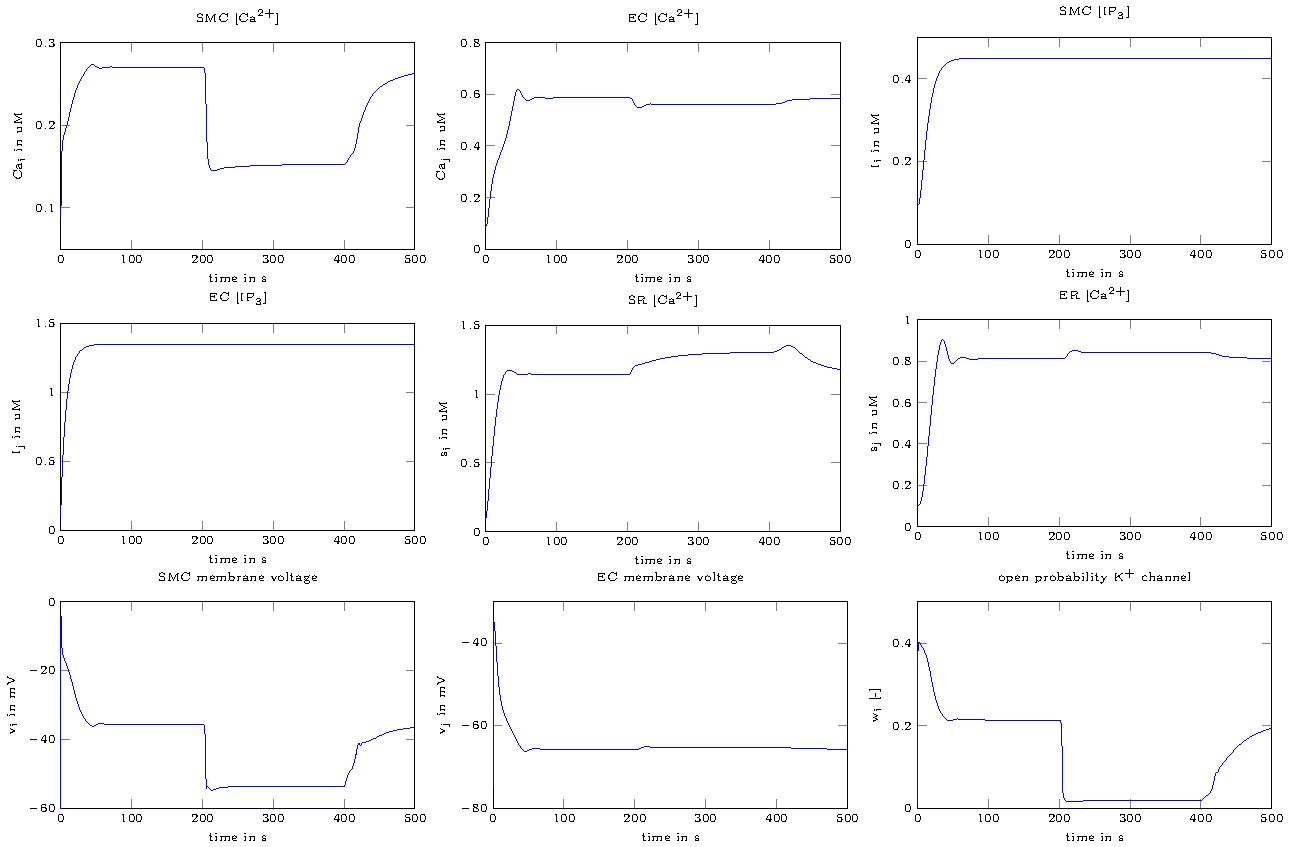
\includegraphics{figures/4_DFDT_new.pdf}
			\caption{Solutions of the differential equations}
			\label{fig:4DFDT}
		\end{figure}
		
		\begin{figure}[h!]
			\centering
			\tiny 
			\setlength\figureheight{3 cm} 
			\setlength\figurewidth{9 cm}
			%% % This file was created by matlab2tikz v0.3.3.
% Copyright (c) 2008--2013, Nico Schlömer <nico.schloemer@gmail.com>
% All rights reserved.
% 
% The latest updates can be retrieved from
%   http://www.mathworks.com/matlabcentral/fileexchange/22022-matlab2tikz
% where you can also make suggestions and rate matlab2tikz.
% 
% 
% 
\begin{tikzpicture}

\begin{axis}[%
width=\figurewidth,
height=\figureheight,
scale only axis,
xmin=0,
xmax=600,
xlabel={Time},
ymin=0,
ymax=0.4,
ylabel={Fraction [-]},
name=plot3,
title={[AMp]}
]
\addplot [
color=blue,
solid,
forget plot
]
table[row sep=crcr]{
0 0.25\\
0.0011996 0.249945049109111\\
0.0023992 0.249890018581467\\
0.0035988 0.249834906933118\\
0.0085566 0.249606343581042\\
0.013514 0.249376438088332\\
0.018472 0.249145181445083\\
0.02343 0.248912579989413\\
0.033542 0.248434035992939\\
0.043655 0.247950066344699\\
0.053767 0.24746079468779\\
0.063879 0.24696634326714\\
0.073991 0.246466830575836\\
0.084819 0.245926492739327\\
0.095647 0.245380626373894\\
0.10647 0.244829371441547\\
0.1173 0.244272866536558\\
0.12813 0.243711248837155\\
0.14659 0.24274243396825\\
0.16505 0.241759820607476\\
0.18351 0.240764067571237\\
0.20197 0.239755828885883\\
0.22042 0.238735758183208\\
0.26398 0.236285915052784\\
0.30753 0.233783164980513\\
0.35108 0.23123804682133\\
0.37397 0.229887233152643\\
0.38969 0.228956459477051\\
0.4054 0.228023368044358\\
0.42111 0.227088493473014\\
0.43393 0.226324133584581\\
0.44676 0.225559087453765\\
0.45959 0.224793539573188\\
0.47242 0.224027662003452\\
0.48525 0.223261617272172\\
0.50035 0.222360078999781\\
0.51544 0.221458766236079\\
0.53054 0.220557912360921\\
0.54564 0.219657742737735\\
0.56073 0.218758475771948\\
0.57728 0.217774452727476\\
0.59382 0.216792038692125\\
0.61036 0.215811495707808\\
0.6269 0.214833077893735\\
0.64344 0.213857031656966\\
0.65998 0.212883595621632\\
0.69992 0.210545572939992\\
0.73986 0.208227141204232\\
0.77979 0.205931113235942\\
0.81973 0.203660034095646\\
0.85967 0.201416196580289\\
0.99616 0.193988086985918\\
1.1327 0.186959535759636\\
1.2692 0.180365879736294\\
1.4056 0.174224865113315\\
1.6062 0.166021885128622\\
1.8067 0.158762892992667\\
2.0072 0.152379693516141\\
2.2078 0.146786851308081\\
2.4083 0.141896483680451\\
2.8551 0.133124516801875\\
3.302 0.12667144193204\\
3.7488 0.121958789536227\\
4.1956 0.118575045978094\\
4.6425 0.116218787095183\\
5.3586 0.114050857876445\\
6.0748 0.113268228094385\\
6.791 0.113462427684429\\
7.5072 0.114396182420704\\
8.2234 0.115902755269638\\
9.2234 0.118731710041448\\
10.223 0.122204994338425\\
11.223 0.126233539925001\\
12.223 0.130767533656479\\
12.523 0.132217805494733\\
12.823 0.133704152201685\\
13.123 0.135223060770539\\
13.423 0.136772643975059\\
13.513 0.137243340825267\\
13.603 0.13771676887621\\
13.693 0.13819288676699\\
13.783 0.138671636993876\\
13.873 0.139152970006245\\
13.929 0.139450778345187\\
13.948 0.139552621657834\\
13.967 0.139654576008345\\
13.986 0.139756640961019\\
14.004 0.139858816092097\\
14.023 0.139961100999285\\
14.079 0.14025981366298\\
14.134 0.1405594453927\\
14.189 0.140859986147309\\
14.244 0.141161425744941\\
14.299 0.141463753867049\\
14.354 0.141766960074247\\
14.409 0.142071033823881\\
14.465 0.142375964482623\\
14.52 0.142683259238854\\
14.575 0.142991397584586\\
14.631 0.143300368356037\\
14.686 0.143610160181881\\
14.742 0.143920761444076\\
14.811 0.144311030232078\\
14.88 0.144702526926596\\
14.95 0.145095226932858\\
15.019 0.145489105086051\\
15.089 0.145884135771864\\
15.202 0.146529282439708\\
15.315 0.147177299083244\\
15.428 0.147828072623503\\
15.541 0.148481490042966\\
15.654 0.149137438783062\\
15.804 0.150013767945762\\
15.954 0.150894114740201\\
16.104 0.151778214978474\\
16.255 0.152665802650261\\
16.405 0.153556608752739\\
16.675 0.15516726420403\\
16.946 0.156785833378104\\
17.216 0.158410652200765\\
17.487 0.160040028941288\\
17.757 0.161672264721717\\
18.061 0.163503941463542\\
18.364 0.165334748143037\\
18.667 0.167162390191648\\
18.971 0.168984634624626\\
19.274 0.170799327896487\\
19.375 0.171400148854424\\
19.476 0.171999836447966\\
19.576 0.17259831989357\\
19.677 0.173195529519032\\
19.778 0.173791397492074\\
19.938 0.174732566168726\\
20.097 0.17566994964617\\
20.257 0.176603306401055\\
20.416 0.177532407428203\\
20.576 0.178457036444856\\
20.994 0.180851602491746\\
21.411 0.183211171663117\\
21.828 0.185533292581637\\
22.056 0.186781932276\\
22.119 0.187129313335352\\
22.183 0.187475740146453\\
22.247 0.187821212753666\\
22.31 0.188165729192943\\
22.432 0.188822510098979\\
22.554 0.189475756357042\\
22.676 0.190125449374942\\
22.798 0.190771574462082\\
22.92 0.191414120975163\\
23.367 0.193742218865575\\
23.684 0.195360816104127\\
24 0.196955384521538\\
24.242 0.198158147555684\\
24.484 0.199347123905148\\
24.726 0.200522479290758\\
24.968 0.201684401678034\\
25.298 0.203247344800961\\
25.628 0.204786227865358\\
25.958 0.20630165177379\\
26.288 0.207794235791787\\
26.618 0.209264601512323\\
27.087 0.211318572084581\\
27.556 0.213330550702753\\
28.025 0.215302149956811\\
28.494 0.217234853994448\\
28.964 0.219130000252931\\
29.615 0.221700793757935\\
30.266 0.224204499725124\\
30.917 0.226643506716871\\
31.569 0.229019915099778\\
32.372 0.231867853375719\\
33.175 0.234626486521654\\
33.979 0.237299359941733\\
34.782 0.239890643133221\\
35.586 0.242405265701958\\
36.23 0.244371461219728\\
36.875 0.246294464470658\\
37.52 0.248176108330345\\
38.164 0.250017185793856\\
38.969 0.252257359555989\\
39.774 0.2544265362815\\
40.579 0.256510534074119\\
41.384 0.258485664458966\\
42.189 0.260318779955148\\
43.189 0.262333727374614\\
44.189 0.263975220860654\\
45.189 0.265160390671087\\
46.189 0.265833912870054\\
47.189 0.265987963091699\\
48.189 0.265672592461914\\
49.189 0.264990607999353\\
50.189 0.264085859406305\\
51.189 0.263088329508187\\
52.189 0.262110040602578\\
53.189 0.261236016602757\\
54.189 0.260517486567797\\
55.189 0.25997486866989\\
56.189 0.259605315017316\\
57.189 0.259392877813058\\
58.189 0.259313013813509\\
59.189 0.2593393724262\\
60.189 0.259448646738188\\
61.189 0.259620250899649\\
62.189 0.259836047379197\\
63.189 0.260080983988347\\
64.189 0.260340499803196\\
65.189 0.260600897053347\\
66.189 0.260850410008928\\
67.189 0.261080020388171\\
68.189 0.261281995888657\\
69.189 0.261444746355613\\
70.189 0.261569408468011\\
71.189 0.26165576957142\\
72.189 0.261709384586736\\
73.189 0.261728940478404\\
74.189 0.261716328972612\\
75.189 0.261675999334532\\
76.189 0.261613776451925\\
77.189 0.261540747953482\\
78.189 0.261462533107972\\
79.189 0.261383030163815\\
80.189 0.261305527964623\\
81.189 0.261231608504047\\
82.189 0.261163035667663\\
83.189 0.261102643667592\\
84.189 0.261052025992162\\
85.189 0.261011860154309\\
86.189 0.260982676259892\\
87.189 0.260960717496929\\
88.189 0.260945071555552\\
89.189 0.260935204650293\\
90.189 0.260930526916431\\
91.189 0.260930171299591\\
92.189 0.260933140225094\\
93.189 0.260938191768532\\
94.189 0.260944150080062\\
95.189 0.260949812021323\\
96.189 0.260954260980906\\
97.189 0.26095668113072\\
98.189 0.260956655249543\\
99.189 0.260953865685951\\
100.19 0.260948392480713\\
101.19 0.260940317704046\\
102.19 0.260930064499651\\
103.19 0.26091792271653\\
104.19 0.260904116260419\\
105.19 0.260889261077982\\
106.19 0.26087401258772\\
107.19 0.260858842662443\\
108.19 0.260844034902221\\
109.19 0.260829823693566\\
110.19 0.260816315968969\\
111.19 0.260803606078478\\
112.19 0.260791693335285\\
113.19 0.260780601783911\\
114.19 0.26077026671857\\
115.19 0.260760674089135\\
116.19 0.260751719649261\\
117.19 0.260743371576843\\
118.19 0.260735500804254\\
119.19 0.260728074427583\\
120.19 0.260720951929835\\
121.19 0.260714115457124\\
122.19 0.260707424910772\\
123.19 0.260700743706874\\
124.19 0.26069403630164\\
125.19 0.260687413612708\\
126.19 0.260680895669027\\
127.19 0.260674446558604\\
128.19 0.260668043479299\\
129.19 0.260661659687023\\
130.19 0.260655288600269\\
131.19 0.260648920941512\\
132.19 0.260642573322717\\
133.19 0.260636252689344\\
134.19 0.26062998919662\\
135.19 0.260623794616297\\
136.19 0.26061770203771\\
137.19 0.260611717716517\\
138.19 0.260605870517782\\
139.19 0.26060015602282\\
140.19 0.260594597029718\\
141.19 0.2605891778048\\
142.19 0.26058391701392\\
143.19 0.26057878940679\\
144.19 0.260573812977199\\
145.19 0.260568955163822\\
146.19 0.260564236712529\\
147.19 0.260559619225419\\
148.19 0.260555128951056\\
149.19 0.260550722087426\\
150.19 0.260546432475138\\
151.19 0.260542210419007\\
152.19 0.260538099047525\\
153.19 0.26053404157641\\
154.19 0.260530091996252\\
155.19 0.26052618467889\\
156.19 0.260522386129085\\
157.19 0.260518619623651\\
158.19 0.260514817418338\\
159.19 0.260510992637453\\
160.19 0.26050728610531\\
161.19 0.260503747075254\\
162.19 0.260500356742347\\
163.19 0.260497098667061\\
164.19 0.260493940750607\\
165.19 0.260490866083868\\
166.19 0.260487846997127\\
167.19 0.260484880887217\\
168.19 0.260481951059999\\
169.19 0.260479067258713\\
170.19 0.260476218739252\\
171.19 0.26047342222658\\
172.19 0.260470666466421\\
173.19 0.260467970677155\\
174.19 0.260465319275509\\
175.19 0.260462732590889\\
176.19 0.260460189535097\\
177.19 0.260457712481454\\
178.19 0.260455275009777\\
179.19 0.260452903309796\\
180.19 0.260450565813147\\
181.19 0.26044829418003\\
182.19 0.260446051241461\\
183.19 0.260443875416337\\
184.19 0.260441722815081\\
185.19 0.260439639746791\\
186.19 0.260437574040535\\
187.19 0.260435581186709\\
188.19 0.260433598926076\\
189.19 0.260431693600353\\
190.19 0.260429790855242\\
191.19 0.260427821465207\\
192.19 0.26042580414562\\
193.19 0.260423874875812\\
194.19 0.260422079345959\\
195.19 0.260420427242453\\
196.19 0.260418877472633\\
196.81 0.260417950238584\\
197.25 0.260417297552125\\
197.57 0.260416824844485\\
197.82 0.260416455272015\\
198.03 0.260416156763936\\
198.24 0.260415860224239\\
198.38 0.260415658889057\\
198.52 0.260415458798723\\
198.63 0.260415301575791\\
198.74 0.260415145407026\\
198.83 0.260415018201225\\
198.92 0.260414891934454\\
199.01 0.260414766749445\\
199.17 0.260414561184685\\
199.32 0.26041435960779\\
199.47 0.260414163267643\\
199.62 0.260413973718499\\
199.84 0.260413713032141\\
200.07 0.260413481507116\\
200.29 0.260413295751111\\
200.51 0.260413151229483\\
200.69 0.260413002274096\\
200.87 0.260412639584738\\
201.05 0.260411690084733\\
201.23 0.260409504805068\\
201.42 0.26040504968885\\
201.6 0.260396561872262\\
201.79 0.260381626877641\\
201.97 0.260356642106927\\
202.15 0.260316435368839\\
202.34 0.260253679863981\\
202.63 0.260081200362993\\
202.92 0.259763333826284\\
203.21 0.259204560310655\\
203.5 0.25826192532026\\
203.79 0.256733069870893\\
204.09 0.254240792548915\\
204.39 0.250474895723403\\
204.69 0.245082714352535\\
204.94 0.239252992379074\\
205.19 0.232141784879854\\
205.44 0.223889156188617\\
205.68 0.214802514149443\\
205.85 0.208245118425637\\
206.02 0.201535219824151\\
206.19 0.194758181949572\\
206.36 0.187986123762256\\
206.6 0.178485034956307\\
206.84 0.169243748424953\\
207.08 0.160358540133964\\
207.32 0.151896267739133\\
207.65 0.140953115427565\\
207.99 0.130950202067081\\
208.32 0.121891840077106\\
208.65 0.113744196592083\\
208.99 0.106454212761463\\
209.66 0.0939967604143606\\
210.18 0.0863147852809455\\
210.7 0.0799715538847023\\
211.22 0.0747402313952057\\
211.74 0.0704259655707243\\
212.26 0.0668646443087306\\
212.9 0.0633042762379216\\
213.54 0.0604770190873341\\
214.18 0.0582191367561659\\
214.82 0.0564060239482707\\
215.46 0.0549426443625084\\
216.16 0.0536538994724838\\
216.87 0.052624864676152\\
217.57 0.0518000119463628\\
218.27 0.0511376085747743\\
218.98 0.050605753733974\\
219.98 0.0500283416596842\\
220.98 0.04961207927197\\
221.98 0.049319067937928\\
222.98 0.0491226063291697\\
223.98 0.0490017831051323\\
224.98 0.0489374109391305\\
225.98 0.048914959837076\\
226.98 0.0489196893809541\\
227.98 0.0489490966730754\\
228.98 0.0489948874759216\\
229.98 0.0490513131729136\\
230.98 0.0491138112820886\\
231.98 0.0491782252089172\\
232.98 0.0492420165943299\\
233.98 0.0493012563871774\\
234.98 0.0493550305999632\\
235.98 0.049403869460944\\
236.98 0.0494483797632179\\
237.98 0.049489900488245\\
238.98 0.0495290361963751\\
239.98 0.0495650965793741\\
240.98 0.0496013229066679\\
241.98 0.0496371483350989\\
242.98 0.0496726394044927\\
243.98 0.0497092025552663\\
244.98 0.0497476588600664\\
245.98 0.0497886253318368\\
246.98 0.049832312497517\\
247.98 0.049878839030522\\
248.98 0.0499281053345552\\
249.98 0.0499799665646234\\
250.98 0.05003415069738\\
251.98 0.0500903617274523\\
252.98 0.0501482334576846\\
253.98 0.0502073957950694\\
254.98 0.0502674518163125\\
255.98 0.0503280220703391\\
256.98 0.0503887339947211\\
257.98 0.0504492505595449\\
258.98 0.0505092642304289\\
259.98 0.0505685136117425\\
260.98 0.0506267779977584\\
261.98 0.0506838852134103\\
262.98 0.0507397054080164\\
263.98 0.0507941528742625\\
264.98 0.0508471790117264\\
265.98 0.0508987704198315\\
266.98 0.0509489415552043\\
267.98 0.050997730976652\\
268.98 0.0510451944292751\\
269.98 0.0510914006865051\\
270.98 0.0511364257060936\\
271.98 0.0511803490380831\\
272.98 0.0512232494444407\\
273.98 0.0512652023866961\\
274.98 0.0513062772148188\\
275.98 0.0513465358760974\\
276.98 0.0513860315400715\\
277.98 0.0514248084077157\\
278.98 0.051462901481423\\
279.98 0.0515003372017502\\
280.98 0.0515371339996442\\
281.98 0.0515733034322668\\
282.98 0.0516088511563696\\
283.98 0.0516437782511539\\
284.98 0.0516780823053519\\
285.98 0.0517117586769366\\
286.98 0.0517448014686436\\
287.98 0.0517772045571361\\
288.98 0.0518089623218157\\
289.98 0.0518400703602873\\
290.98 0.0518705259178112\\
291.98 0.0519003282781175\\
292.98 0.0519294789058477\\
293.98 0.0519579815543765\\
294.98 0.0519858421766162\\
295.98 0.0520130688221662\\
296.98 0.0520396713929665\\
297.98 0.0520656614125266\\
298.98 0.0520910517054591\\
299.98 0.0521158561160808\\
300.98 0.0521400891800467\\
301.98 0.0521637658538237\\
302.98 0.0521869012282204\\
303.98 0.0522095103096595\\
304.98 0.0522316078045748\\
305.98 0.0522532079727052\\
306.98 0.0522743244921346\\
307.98 0.0522949703872705\\
308.98 0.0523151579692798\\
309.98 0.0523348988287935\\
310.98 0.0523542038367462\\
311.98 0.0523730831846335\\
312.98 0.0523915464262349\\
313.98 0.0524096025459209\\
314.98 0.0524272600215636\\
315.98 0.0524445269028214\\
316.98 0.0524614108784331\\
317.98 0.0524779193502326\\
318.98 0.0524940594926104\\
319.98 0.0525098383129044\\
320.98 0.0525252626958758\\
321.98 0.0525403394459992\\
322.98 0.0525550753144119\\
323.98 0.0525694770227319\\
324.98 0.052583551273528\\
325.98 0.0525973047582208\\
326.98 0.0526107441544411\\
327.98 0.0526238761222188\\
328.98 0.0526367072926742\\
329.98 0.0526492442572019\\
330.98 0.0526614935519882\\
331.98 0.0526734616445205\\
332.98 0.0526851549177462\\
333.98 0.0526965796573068\\
334.98 0.0527077420380829\\
335.98 0.0527186481143772\\
336.98 0.0527293038104096\\
337.98 0.0527397149145125\\
338.98 0.0527498870740687\\
339.98 0.0527598257938132\\
340.98 0.0527695364348775\\
341.98 0.0527790242166046\\
342.98 0.0527882942188363\\
343.98 0.0527973513862618\\
344.98 0.0528062005328492\\
345.98 0.0528148463476345\\
346.98 0.0528232934002012\\
347.98 0.0528315461469082\\
348.98 0.0528396089364947\\
349.98 0.0528474860159638\\
350.98 0.052855181535651\\
351.98 0.0528626995542591\\
352.98 0.0528700440430085\\
353.98 0.0528772188895925\\
354.98 0.0528842279012837\\
355.98 0.0528910748078028\\
356.98 0.0528977632634521\\
357.98 0.0529042968490508\\
358.98 0.0529106790732915\\
359.98 0.0529169133739812\\
360.98 0.0529230031188733\\
361.98 0.0529289516064793\\
362.98 0.0529347620666257\\
363.98 0.0529404376610781\\
364.98 0.0529459814840344\\
365.98 0.0529513965627483\\
366.98 0.0529566858581095\\
367.98 0.0529618522653872\\
368.98 0.0529668986149832\\
369.98 0.0529718276733516\\
370.98 0.0529766421439507\\
371.98 0.0529813446683439\\
372.98 0.0529859378273285\\
373.98 0.0529904241421866\\
374.98 0.0529948060759424\\
375.98 0.0529990860347081\\
376.98 0.0530032663690118\\
377.98 0.0530073493751771\\
378.98 0.0530113372966626\\
379.98 0.0530152323254229\\
380.98 0.0530190366032095\\
381.98 0.0530227522228707\\
382.98 0.0530263812295816\\
383.98 0.0530299256220561\\
384.98 0.0530333873536868\\
385.98 0.0530367683336583\\
386.98 0.0530400704279924\\
387.98 0.0530432954605644\\
388.98 0.0530464452140597\\
389.98 0.053049521430905\\
390.98 0.053052525814169\\
391.98 0.0530554600285655\\
392.98 0.0530583257023668\\
393.98 0.0530611244362825\\
394.98 0.0530638578639368\\
395.98 0.0530665280936268\\
396.98 0.0530691409592062\\
397.98 0.0530717361391083\\
398.44 0.0530729084820033\\
398.8 0.0530738081290685\\
399.07 0.0530744803531493\\
399.35 0.0530751263232932\\
399.55 0.0530755927343881\\
399.76 0.0530760520730591\\
399.96 0.0530765060068809\\
400.26 0.0530774526099009\\
400.34 0.0530778446225945\\
400.43 0.0530783655682202\\
400.52 0.0530790794141504\\
400.61 0.0530800650173538\\
400.92 0.053087969229545\\
401.24 0.0531054823037959\\
401.56 0.0531372907133649\\
401.87 0.0531879820789268\\
402.11 0.0532414458867301\\
402.35 0.0533097272542623\\
402.59 0.0533940127453636\\
402.83 0.0534951651457415\\
403.14 0.0536521027035536\\
403.45 0.0538388469280014\\
403.77 0.0540552674599237\\
404.08 0.0543005405363544\\
404.39 0.0545733038322666\\
404.93 0.0551100110497551\\
405.47 0.0557141500593873\\
406.02 0.0563734689950981\\
406.56 0.0570753866149553\\
407.1 0.0578079701310321\\
408.1 0.0592006315042732\\
408.77 0.0601303819815365\\
409.43 0.0610416100541704\\
410.1 0.0619183836836236\\
410.61 0.0625646165604033\\
411.12 0.0631880834569027\\
411.63 0.0637996277738873\\
412.15 0.0644165243117745\\
412.66 0.0650589196990349\\
413.31 0.065937605993121\\
413.95 0.0669248068404595\\
414.6 0.0680523400635156\\
415.25 0.0693494467886148\\
415.9 0.0708460427186867\\
416.77 0.073251489831406\\
417.65 0.0761889931252293\\
418.52 0.0797809875921216\\
419.4 0.0841422093132543\\
420.28 0.0892932478209126\\
421.2 0.0953589211525189\\
422.12 0.101584490439819\\
423.04 0.107355061396884\\
423.96 0.112312273746438\\
424.89 0.116611691296581\\
425.81 0.12075603641087\\
426.73 0.125131043650348\\
427.68 0.129878821943447\\
428.64 0.134593977142136\\
429.59 0.139057619006262\\
430.55 0.143258548634496\\
431.5 0.147336166128069\\
432.5 0.151600196249748\\
433.5 0.155842136535492\\
434.5 0.159953877655649\\
435.5 0.163863210243302\\
436.5 0.167582006974461\\
437.5 0.171169104416903\\
438.5 0.174647812870073\\
439.5 0.177986301478357\\
440.5 0.18114284551824\\
441.5 0.184112983132373\\
442.5 0.186913568988881\\
443.5 0.189513245052309\\
444.5 0.191955718282661\\
445.5 0.194256265520757\\
446.5 0.196427073212316\\
447.5 0.198478556834493\\
448.5 0.200437613420899\\
449.5 0.202300984869319\\
450.5 0.204066941932385\\
451.5 0.20573890229498\\
452.5 0.207323864636302\\
453.5 0.208830256220001\\
454.5 0.210266452656557\\
455.5 0.211639993035848\\
456.5 0.212957289278476\\
457.5 0.214223651722406\\
458.5 0.21544345095393\\
459.5 0.216620309758941\\
460.5 0.217757274379765\\
461.5 0.218856944612164\\
462.5 0.219921568173917\\
463.5 0.220953108454917\\
464.5 0.22195329393833\\
465.5 0.222923656530172\\
466.5 0.223865562059184\\
467.5 0.224780235352393\\
468.5 0.225668781379806\\
469.5 0.226532203060275\\
470.5 0.227371416558346\\
471.5 0.228187264404625\\
472.5 0.228980526734851\\
473.5 0.229751930981887\\
474.5 0.23050216010323\\
475.5 0.231231859572223\\
476.5 0.231941643253561\\
477.5 0.232632098255323\\
478.5 0.23330378891833\\
479.5 0.233957259989524\\
480.5 0.234593039097428\\
481.5 0.235211638613724\\
482.5 0.235813556963229\\
483.5 0.236399279501391\\
484.5 0.236969279015506\\
485.5 0.237524015952419\\
486.5 0.238063938455502\\
487.5 0.238589482268579\\
488.5 0.239101070596274\\
489.5 0.239599113949768\\
490.5 0.24008401003288\\
491.5 0.240556143696768\\
492.5 0.241015886968283\\
493.5 0.241463599182226\\
494.5 0.241899627195752\\
495.5 0.242324305695732\\
496.5 0.242737957584634\\
497.5 0.243140894422034\\
498.5 0.243533416925894\\
499.5 0.243915815492132\\
500 0.244102704753535\\
};
\end{axis}

\begin{axis}[%
width=\figurewidth,
height=\figureheight,
scale only axis,
xmin=0,
xmax=600,
xlabel={Time},
ymin=0,
ymax=1,
ylabel={Fraction [-]},
name=plot1,
at=(plot3.above north west),
anchor=below south west,
title={[M]}
]
\addplot [
color=blue,
solid,
forget plot
]
table[row sep=crcr]{
0 0.25\\
0.0011996 0.25017\\
0.0023992 0.25035\\
0.0035988 0.25052\\
0.0085566 0.25124\\
0.013514 0.25196\\
0.018472 0.25268\\
0.02343 0.25339\\
0.033542 0.25484\\
0.043655 0.25628\\
0.053767 0.25772\\
0.063879 0.25914\\
0.073991 0.26056\\
0.084819 0.26207\\
0.095647 0.26357\\
0.10647 0.26506\\
0.1173 0.26654\\
0.12813 0.26801\\
0.14659 0.27051\\
0.16505 0.27297\\
0.18351 0.27541\\
0.20197 0.27782\\
0.22042 0.28022\\
0.26398 0.28576\\
0.30753 0.29117\\
0.35108 0.29645\\
0.37397 0.29917\\
0.38969 0.30101\\
0.4054 0.30284\\
0.42111 0.30465\\
0.43393 0.30611\\
0.44676 0.30756\\
0.45959 0.309\\
0.47242 0.31043\\
0.48525 0.31184\\
0.50035 0.31349\\
0.51544 0.31512\\
0.53054 0.31674\\
0.54564 0.31834\\
0.56073 0.31993\\
0.57728 0.32165\\
0.59382 0.32335\\
0.61036 0.32503\\
0.6269 0.32669\\
0.64344 0.32833\\
0.65998 0.32996\\
0.69992 0.33381\\
0.73986 0.33755\\
0.77979 0.34119\\
0.81973 0.34474\\
0.85967 0.34818\\
0.99616 0.35927\\
1.1327 0.36934\\
1.2692 0.37848\\
1.4056 0.38678\\
1.6062 0.39763\\
1.8067 0.40712\\
2.0072 0.41548\\
2.2078 0.42293\\
2.4083 0.42962\\
2.8551 0.44241\\
3.302 0.45313\\
3.7488 0.46239\\
4.1956 0.4705\\
4.6425 0.47762\\
5.3586 0.48727\\
6.0748 0.49506\\
6.791 0.50115\\
7.5072 0.50565\\
8.2234 0.50869\\
9.2234 0.51072\\
10.223 0.51047\\
11.223 0.50812\\
12.223 0.5039\\
12.523 0.50231\\
12.823 0.50058\\
13.123 0.49873\\
13.423 0.49676\\
13.513 0.49615\\
13.603 0.49553\\
13.693 0.49489\\
13.783 0.49425\\
13.873 0.4936\\
13.929 0.49319\\
13.948 0.49305\\
13.967 0.49291\\
13.986 0.49277\\
14.004 0.49263\\
14.023 0.49249\\
14.079 0.49207\\
14.134 0.49166\\
14.189 0.49124\\
14.244 0.49081\\
14.299 0.49038\\
14.354 0.48995\\
14.409 0.48952\\
14.465 0.48908\\
14.52 0.48864\\
14.575 0.4882\\
14.631 0.48775\\
14.686 0.4873\\
14.742 0.48684\\
14.811 0.48627\\
14.88 0.48569\\
14.95 0.48511\\
15.019 0.48452\\
15.089 0.48393\\
15.202 0.48296\\
15.315 0.48198\\
15.428 0.48099\\
15.541 0.47998\\
15.654 0.47897\\
15.804 0.47762\\
15.954 0.47624\\
16.104 0.47485\\
16.255 0.47345\\
16.405 0.47203\\
16.675 0.46946\\
16.946 0.46685\\
17.216 0.4642\\
17.487 0.46154\\
17.757 0.45885\\
18.061 0.45582\\
18.364 0.45277\\
18.667 0.44972\\
18.971 0.44666\\
19.274 0.44361\\
19.375 0.44259\\
19.476 0.44158\\
19.576 0.44057\\
19.677 0.43956\\
19.778 0.43855\\
19.938 0.43696\\
20.097 0.43537\\
20.257 0.43379\\
20.416 0.43221\\
20.576 0.43064\\
20.994 0.42656\\
21.411 0.42254\\
21.828 0.41859\\
22.056 0.41646\\
22.119 0.41587\\
22.183 0.41528\\
22.247 0.41469\\
22.31 0.4141\\
22.432 0.41298\\
22.554 0.41187\\
22.676 0.41077\\
22.798 0.40967\\
22.92 0.40857\\
23.367 0.40462\\
23.684 0.40187\\
24 0.39917\\
24.242 0.39714\\
24.484 0.39513\\
24.726 0.39315\\
24.968 0.3912\\
25.298 0.38858\\
25.628 0.38601\\
25.958 0.38349\\
26.288 0.38101\\
26.618 0.37859\\
27.087 0.37522\\
27.556 0.37194\\
28.025 0.36875\\
28.494 0.36564\\
28.964 0.36262\\
29.615 0.35856\\
30.266 0.35465\\
30.917 0.35089\\
31.569 0.34726\\
32.372 0.34297\\
33.175 0.33887\\
33.979 0.33495\\
34.782 0.3312\\
35.586 0.32761\\
36.23 0.32483\\
36.875 0.32214\\
37.52 0.31954\\
38.164 0.31702\\
38.969 0.31399\\
39.774 0.31108\\
40.579 0.30831\\
41.384 0.30569\\
42.189 0.30326\\
43.189 0.30056\\
44.189 0.29827\\
45.189 0.29649\\
46.189 0.29526\\
47.189 0.2946\\
48.189 0.29447\\
49.189 0.29478\\
50.189 0.29539\\
51.189 0.29619\\
52.189 0.29706\\
53.189 0.29791\\
54.189 0.29867\\
55.189 0.2993\\
56.189 0.29979\\
57.189 0.30014\\
58.189 0.30035\\
59.189 0.30044\\
60.189 0.30043\\
61.189 0.30033\\
62.189 0.30017\\
63.189 0.29996\\
64.189 0.29972\\
65.189 0.29946\\
66.189 0.2992\\
67.189 0.29894\\
68.189 0.29871\\
69.189 0.29851\\
70.189 0.29835\\
71.189 0.29822\\
72.189 0.29812\\
73.189 0.29807\\
74.189 0.29804\\
75.189 0.29806\\
76.189 0.2981\\
77.189 0.29816\\
78.189 0.29823\\
79.189 0.2983\\
80.189 0.29838\\
81.189 0.29846\\
82.189 0.29853\\
83.189 0.2986\\
84.189 0.29867\\
85.189 0.29872\\
86.189 0.29876\\
87.189 0.29879\\
88.189 0.29882\\
89.189 0.29884\\
90.189 0.29885\\
91.189 0.29886\\
92.189 0.29886\\
93.189 0.29886\\
94.189 0.29886\\
95.189 0.29886\\
96.189 0.29885\\
97.189 0.29885\\
98.189 0.29885\\
99.189 0.29886\\
100.19 0.29886\\
101.19 0.29887\\
102.19 0.29888\\
103.19 0.29889\\
104.19 0.29891\\
105.19 0.29892\\
106.19 0.29894\\
107.19 0.29895\\
108.19 0.29897\\
109.19 0.29899\\
110.19 0.299\\
111.19 0.29902\\
112.19 0.29903\\
113.19 0.29905\\
114.19 0.29906\\
115.19 0.29907\\
116.19 0.29908\\
117.19 0.29909\\
118.19 0.2991\\
119.19 0.29911\\
120.19 0.29912\\
121.19 0.29913\\
122.19 0.29914\\
123.19 0.29915\\
124.19 0.29916\\
125.19 0.29917\\
126.19 0.29917\\
127.19 0.29918\\
128.19 0.29919\\
129.19 0.2992\\
130.19 0.29921\\
131.19 0.29921\\
132.19 0.29922\\
133.19 0.29923\\
134.19 0.29924\\
135.19 0.29924\\
136.19 0.29925\\
137.19 0.29926\\
138.19 0.29926\\
139.19 0.29927\\
140.19 0.29928\\
141.19 0.29929\\
142.19 0.29929\\
143.19 0.2993\\
144.19 0.2993\\
145.19 0.29931\\
146.19 0.29932\\
147.19 0.29932\\
148.19 0.29933\\
149.19 0.29933\\
150.19 0.29934\\
151.19 0.29934\\
152.19 0.29935\\
153.19 0.29935\\
154.19 0.29936\\
155.19 0.29936\\
156.19 0.29937\\
157.19 0.29937\\
158.19 0.29938\\
159.19 0.29938\\
160.19 0.29939\\
161.19 0.29939\\
162.19 0.29939\\
163.19 0.2994\\
164.19 0.2994\\
165.19 0.29941\\
166.19 0.29941\\
167.19 0.29941\\
168.19 0.29942\\
169.19 0.29942\\
170.19 0.29942\\
171.19 0.29943\\
172.19 0.29943\\
173.19 0.29943\\
174.19 0.29944\\
175.19 0.29944\\
176.19 0.29944\\
177.19 0.29945\\
178.19 0.29945\\
179.19 0.29945\\
180.19 0.29946\\
181.19 0.29946\\
182.19 0.29946\\
183.19 0.29946\\
184.19 0.29947\\
185.19 0.29947\\
186.19 0.29947\\
187.19 0.29947\\
188.19 0.29948\\
189.19 0.29948\\
190.19 0.29948\\
191.19 0.29948\\
192.19 0.29949\\
193.19 0.29949\\
194.19 0.29949\\
195.19 0.29949\\
196.19 0.29949\\
196.81 0.2995\\
197.25 0.2995\\
197.57 0.2995\\
197.82 0.2995\\
198.03 0.2995\\
198.24 0.2995\\
198.38 0.2995\\
198.52 0.2995\\
198.63 0.2995\\
198.74 0.2995\\
198.83 0.2995\\
198.92 0.2995\\
199.01 0.2995\\
199.17 0.2995\\
199.32 0.2995\\
199.47 0.2995\\
199.62 0.2995\\
199.84 0.2995\\
200.07 0.2995\\
200.29 0.2995\\
200.51 0.2995\\
200.69 0.2995\\
200.87 0.2995\\
201.05 0.2995\\
201.23 0.29951\\
201.42 0.29951\\
201.6 0.29952\\
201.79 0.29953\\
201.97 0.29956\\
202.15 0.2996\\
202.34 0.29966\\
202.63 0.29982\\
202.92 0.30013\\
203.21 0.30066\\
203.5 0.30156\\
203.79 0.30303\\
204.09 0.30542\\
204.39 0.30903\\
204.69 0.31421\\
204.94 0.31982\\
205.19 0.3267\\
205.44 0.33472\\
205.68 0.34364\\
205.85 0.35013\\
206.02 0.35684\\
206.19 0.36369\\
206.36 0.37064\\
206.6 0.38059\\
206.84 0.39054\\
207.08 0.4004\\
207.32 0.41014\\
207.65 0.42334\\
207.99 0.43615\\
208.32 0.44856\\
208.65 0.46055\\
208.99 0.47212\\
209.66 0.49437\\
210.18 0.5103\\
210.7 0.52532\\
211.22 0.53946\\
211.74 0.55279\\
212.26 0.56533\\
212.9 0.5798\\
213.54 0.59322\\
214.18 0.60564\\
214.82 0.61713\\
215.46 0.62775\\
216.16 0.63846\\
216.87 0.64826\\
217.57 0.65722\\
218.27 0.66539\\
218.98 0.67283\\
219.98 0.68227\\
220.98 0.69049\\
221.98 0.69763\\
222.98 0.70381\\
223.98 0.70914\\
224.98 0.71374\\
225.98 0.71768\\
226.98 0.72105\\
227.98 0.72393\\
228.98 0.72637\\
229.98 0.72844\\
230.98 0.73019\\
231.98 0.73166\\
232.98 0.73291\\
233.98 0.73396\\
234.98 0.73485\\
235.98 0.73559\\
236.98 0.73622\\
237.98 0.73674\\
238.98 0.73716\\
239.98 0.7375\\
240.98 0.73778\\
241.98 0.73801\\
242.98 0.73818\\
243.98 0.73832\\
244.98 0.73841\\
245.98 0.73846\\
246.98 0.73848\\
247.98 0.73846\\
248.98 0.73842\\
249.98 0.73836\\
250.98 0.73827\\
251.98 0.73816\\
252.98 0.73804\\
253.98 0.7379\\
254.98 0.73774\\
255.98 0.73758\\
256.98 0.7374\\
257.98 0.73722\\
258.98 0.73704\\
259.98 0.73685\\
260.98 0.73665\\
261.98 0.73646\\
262.98 0.73626\\
263.98 0.73607\\
264.98 0.73587\\
265.98 0.73568\\
266.98 0.73549\\
267.98 0.73531\\
268.98 0.73512\\
269.98 0.73494\\
270.98 0.73476\\
271.98 0.73459\\
272.98 0.73442\\
273.98 0.73425\\
274.98 0.73408\\
275.98 0.73392\\
276.98 0.73376\\
277.98 0.7336\\
278.98 0.73345\\
279.98 0.73329\\
280.98 0.73314\\
281.98 0.733\\
282.98 0.73285\\
283.98 0.73271\\
284.98 0.73257\\
285.98 0.73244\\
286.98 0.7323\\
287.98 0.73217\\
288.98 0.73204\\
289.98 0.73191\\
290.98 0.73179\\
291.98 0.73167\\
292.98 0.73155\\
293.98 0.73143\\
294.98 0.73132\\
295.98 0.73121\\
296.98 0.7311\\
297.98 0.73099\\
298.98 0.73089\\
299.98 0.73078\\
300.98 0.73068\\
301.98 0.73059\\
302.98 0.73049\\
303.98 0.7304\\
304.98 0.73031\\
305.98 0.73022\\
306.98 0.73013\\
307.98 0.73005\\
308.98 0.72996\\
309.98 0.72988\\
310.98 0.7298\\
311.98 0.72972\\
312.98 0.72965\\
313.98 0.72957\\
314.98 0.7295\\
315.98 0.72943\\
316.98 0.72936\\
317.98 0.72929\\
318.98 0.72923\\
319.98 0.72916\\
320.98 0.7291\\
321.98 0.72903\\
322.98 0.72897\\
323.98 0.72891\\
324.98 0.72886\\
325.98 0.7288\\
326.98 0.72875\\
327.98 0.72869\\
328.98 0.72864\\
329.98 0.72859\\
330.98 0.72854\\
331.98 0.72849\\
332.98 0.72844\\
333.98 0.72839\\
334.98 0.72835\\
335.98 0.7283\\
336.98 0.72826\\
337.98 0.72821\\
338.98 0.72817\\
339.98 0.72813\\
340.98 0.72809\\
341.98 0.72805\\
342.98 0.72801\\
343.98 0.72798\\
344.98 0.72794\\
345.98 0.72791\\
346.98 0.72787\\
347.98 0.72784\\
348.98 0.7278\\
349.98 0.72777\\
350.98 0.72774\\
351.98 0.72771\\
352.98 0.72768\\
353.98 0.72765\\
354.98 0.72762\\
355.98 0.72759\\
356.98 0.72756\\
357.98 0.72754\\
358.98 0.72751\\
359.98 0.72749\\
360.98 0.72746\\
361.98 0.72744\\
362.98 0.72741\\
363.98 0.72739\\
364.98 0.72737\\
365.98 0.72734\\
366.98 0.72732\\
367.98 0.7273\\
368.98 0.72728\\
369.98 0.72726\\
370.98 0.72724\\
371.98 0.72722\\
372.98 0.7272\\
373.98 0.72718\\
374.98 0.72717\\
375.98 0.72715\\
376.98 0.72713\\
377.98 0.72711\\
378.98 0.7271\\
379.98 0.72708\\
380.98 0.72707\\
381.98 0.72705\\
382.98 0.72704\\
383.98 0.72702\\
384.98 0.72701\\
385.98 0.72699\\
386.98 0.72698\\
387.98 0.72697\\
388.98 0.72695\\
389.98 0.72694\\
390.98 0.72693\\
391.98 0.72692\\
392.98 0.7269\\
393.98 0.72689\\
394.98 0.72688\\
395.98 0.72687\\
396.98 0.72686\\
397.98 0.72685\\
398.44 0.72684\\
398.8 0.72684\\
399.07 0.72684\\
399.35 0.72684\\
399.55 0.72683\\
399.76 0.72683\\
399.96 0.72683\\
400.26 0.72683\\
400.34 0.72682\\
400.43 0.72682\\
400.52 0.72682\\
400.61 0.72682\\
400.92 0.72679\\
401.24 0.72673\\
401.56 0.72664\\
401.87 0.7265\\
402.11 0.72635\\
402.35 0.72617\\
402.59 0.72595\\
402.83 0.7257\\
403.14 0.72531\\
403.45 0.72486\\
403.77 0.72434\\
404.08 0.72376\\
404.39 0.72311\\
404.93 0.72185\\
405.47 0.72043\\
406.02 0.71887\\
406.56 0.71719\\
407.1 0.7154\\
408.1 0.71191\\
408.77 0.7095\\
409.43 0.70706\\
410.1 0.70464\\
410.61 0.70279\\
411.12 0.70095\\
411.63 0.69909\\
412.15 0.69717\\
412.66 0.69517\\
413.31 0.69246\\
413.95 0.68948\\
414.6 0.68619\\
415.25 0.68253\\
415.9 0.67843\\
416.77 0.67204\\
417.65 0.66448\\
418.52 0.6555\\
419.4 0.64487\\
420.28 0.63264\\
421.2 0.61857\\
422.12 0.60433\\
423.04 0.59101\\
423.96 0.57905\\
424.89 0.56802\\
425.81 0.55712\\
426.73 0.54594\\
427.68 0.53437\\
428.64 0.52325\\
429.59 0.51284\\
430.55 0.50303\\
431.5 0.49359\\
432.5 0.48399\\
433.5 0.47473\\
434.5 0.46596\\
435.5 0.45773\\
436.5 0.44998\\
437.5 0.44262\\
438.5 0.43563\\
439.5 0.42905\\
440.5 0.4229\\
441.5 0.41717\\
442.5 0.41182\\
443.5 0.40691\\
444.5 0.40235\\
445.5 0.3981\\
446.5 0.39413\\
447.5 0.39042\\
448.5 0.38691\\
449.5 0.3836\\
450.5 0.38051\\
451.5 0.37761\\
452.5 0.3749\\
453.5 0.37235\\
454.5 0.36995\\
455.5 0.36768\\
456.5 0.36553\\
457.5 0.36348\\
458.5 0.36154\\
459.5 0.35968\\
460.5 0.3579\\
461.5 0.3562\\
462.5 0.35457\\
463.5 0.353\\
464.5 0.3515\\
465.5 0.35004\\
466.5 0.34864\\
467.5 0.34729\\
468.5 0.34599\\
469.5 0.34473\\
470.5 0.34351\\
471.5 0.34233\\
472.5 0.34119\\
473.5 0.34009\\
474.5 0.33902\\
475.5 0.33798\\
476.5 0.33698\\
477.5 0.336\\
478.5 0.33506\\
479.5 0.33415\\
480.5 0.33326\\
481.5 0.3324\\
482.5 0.33157\\
483.5 0.33076\\
484.5 0.32997\\
485.5 0.32921\\
486.5 0.32847\\
487.5 0.32775\\
488.5 0.32705\\
489.5 0.32638\\
490.5 0.32572\\
491.5 0.32508\\
492.5 0.32446\\
493.5 0.32385\\
494.5 0.32327\\
495.5 0.3227\\
496.5 0.32214\\
497.5 0.32161\\
498.5 0.32108\\
499.5 0.32057\\
500 0.32033\\
};
\end{axis}

\begin{axis}[%
width=\figurewidth,
height=\figureheight,
scale only axis,
xmin=0,
xmax=600,
xlabel={Time},
ymin=0,
ymax=0.4,
ylabel={Fraction [-]},
name=plot2,
at=(plot1.right of south east),
anchor=left of south west,
title={[Mp]}
]
\addplot [
color=blue,
solid,
forget plot
]
table[row sep=crcr]{
0 0.25\\
0.0011996 0.249765379432397\\
0.0023992 0.249530991998954\\
0.0035988 0.24929684238333\\
0.0085566 0.248331475533219\\
0.013514 0.247370072424635\\
0.018472 0.246412683550287\\
0.02343 0.245459315725906\\
0.033542 0.243527158351838\\
0.043655 0.241611553374092\\
0.053767 0.23971235637645\\
0.063879 0.237829424129683\\
0.073991 0.235962621059602\\
0.084819 0.233981454704566\\
0.095647 0.232018470514128\\
0.10647 0.230073509761544\\
0.1173 0.228146415326077\\
0.12813 0.226237032148786\\
0.14659 0.223022427373591\\
0.16505 0.219858109907992\\
0.18351 0.216743358037774\\
0.20197 0.213677473772419\\
0.22042 0.210659785943371\\
0.26398 0.203727177858466\\
0.30753 0.197052214363433\\
0.35108 0.190629707150235\\
0.37397 0.187353873725398\\
0.38969 0.185145691108858\\
0.4054 0.182969971465479\\
0.42111 0.1808265864257\\
0.43393 0.179100286029926\\
0.44676 0.177395254896401\\
0.45959 0.175711328229203\\
0.47242 0.174048332516162\\
0.48525 0.172406088655592\\
0.50035 0.170499718541864\\
0.51544 0.168621537583002\\
0.53054 0.166771244817579\\
0.54564 0.164948539592301\\
0.56073 0.163153122436625\\
0.57728 0.161216892533606\\
0.59382 0.159312675761753\\
0.61036 0.157440086017112\\
0.6269 0.155598740344294\\
0.64344 0.153788258883312\\
0.65998 0.152008264747641\\
0.69992 0.14783427113127\\
0.73986 0.143830607064719\\
0.77979 0.139992147974246\\
0.81973 0.136313849214631\\
0.85967 0.132790740530174\\
0.99616 0.12182830014539\\
1.1327 0.112432612531259\\
1.2692 0.104431299893854\\
1.4056 0.0976557425814279\\
1.6062 0.0896182371397627\\
1.8067 0.0834549112565042\\
2.0072 0.0787758060265365\\
2.2078 0.0752647911627785\\
2.4083 0.0726703460350161\\
2.8551 0.0692983126097257\\
3.302 0.0679750255050869\\
3.7488 0.0678009403502595\\
4.1956 0.0683359975290703\\
4.6425 0.0693384377208329\\
5.3586 0.0715436157975951\\
6.0748 0.0741249665977164\\
6.791 0.076928854179777\\
7.5072 0.0799054569946044\\
8.2234 0.0829954304660825\\
9.2234 0.0873770533822776\\
10.223 0.0917694402841623\\
11.223 0.0961826777967158\\
12.223 0.10059067779194\\
12.523 0.101902391879551\\
12.823 0.103200676416612\\
13.123 0.104483578299925\\
13.423 0.10575147208481\\
13.513 0.106129088426645\\
13.603 0.106505537024835\\
13.693 0.106880768054412\\
13.783 0.107254718819923\\
13.873 0.107627344556943\\
13.929 0.107856239105256\\
13.948 0.107934228406046\\
13.967 0.108012156962206\\
13.986 0.108090024375136\\
14.004 0.108167830278769\\
14.023 0.1082455743481\\
14.079 0.108471789283684\\
14.134 0.108697468480104\\
14.189 0.108922603931358\\
14.244 0.109147187519771\\
14.299 0.109371211030306\\
14.354 0.109594666182076\\
14.409 0.109817544663717\\
14.465 0.110039838159449\\
14.52 0.110262635887768\\
14.575 0.110484825916666\\
14.631 0.11070639962983\\
14.686 0.110927348209122\\
14.742 0.111147662574424\\
14.811 0.111422779574317\\
14.88 0.11169686729406\\
14.95 0.111969906155145\\
15.019 0.11224187617213\\
15.089 0.112512757188831\\
15.202 0.112951125984557\\
15.315 0.113386474276646\\
15.428 0.113818720684006\\
15.541 0.114247787963324\\
15.654 0.114673603171698\\
15.804 0.11523490007042\\
15.954 0.115790164933007\\
16.104 0.116339249269309\\
16.255 0.116882008959728\\
16.405 0.117418301929497\\
16.675 0.118366865274717\\
16.946 0.119293199608826\\
17.216 0.120196504985716\\
17.487 0.121076026142016\\
17.757 0.121931080792582\\
18.061 0.122860092878202\\
18.364 0.12375691305579\\
18.667 0.124621003639003\\
18.971 0.125451973077453\\
19.274 0.126249587661249\\
19.375 0.126507155057157\\
19.476 0.126761036418543\\
19.576 0.127011235675\\
19.677 0.127257757955957\\
19.778 0.127500611039506\\
19.938 0.12787789537368\\
20.097 0.128246048140524\\
20.257 0.128605133690176\\
20.416 0.128955229391576\\
20.576 0.129296425121466\\
20.994 0.130147602979468\\
21.411 0.13094101835956\\
21.828 0.131679220870548\\
22.056 0.132058943781039\\
22.119 0.132162497091226\\
22.183 0.132264893962466\\
22.247 0.132366141970795\\
22.31 0.132466251179425\\
22.432 0.132654741975084\\
22.554 0.13283918836436\\
22.676 0.13301968041797\\
22.798 0.133196308693739\\
22.92 0.13336916330569\\
23.367 0.133973476030151\\
23.684 0.134373406391379\\
24 0.134752205747458\\
24.242 0.135028366567732\\
24.484 0.135293743911678\\
24.726 0.135548979665816\\
24.968 0.135794690979869\\
25.298 0.136115367444885\\
25.628 0.136420832620158\\
25.958 0.13671247091267\\
26.288 0.136991546958382\\
26.618 0.137259208558496\\
27.087 0.137622201890355\\
27.556 0.137966881165059\\
28.025 0.138295557675621\\
28.494 0.138610173966701\\
28.964 0.138912345997064\\
29.615 0.139313955477913\\
30.266 0.139697044441079\\
30.917 0.140063873028907\\
31.569 0.140416241359052\\
32.372 0.140832998004755\\
33.175 0.141232134850423\\
33.979 0.141615830359406\\
34.782 0.141986471204432\\
35.586 0.142346733066947\\
36.23 0.142630102729206\\
36.875 0.14290937764974\\
37.52 0.143184808956768\\
38.164 0.143455774337498\\
38.969 0.143785086370656\\
39.774 0.144097938589111\\
40.579 0.144382750440572\\
41.384 0.144622970483871\\
42.189 0.144797777347863\\
43.189 0.144889842684061\\
44.189 0.144805088150465\\
45.189 0.144515168555402\\
46.189 0.144016817880045\\
47.189 0.143339467318828\\
48.189 0.142543702769701\\
49.189 0.141709952100126\\
50.189 0.1409265855559\\
51.189 0.140249695972197\\
52.189 0.139717713553253\\
53.189 0.139346559712861\\
54.189 0.139130725785698\\
55.189 0.139048789430664\\
56.189 0.139071460842038\\
57.189 0.139170504619273\\
58.189 0.139316762146742\\
59.189 0.139487313909998\\
60.189 0.139666699739562\\
61.189 0.139844885214726\\
62.189 0.140014755598872\\
63.189 0.140171355128136\\
64.189 0.140310083410299\\
65.189 0.140427362061344\\
66.189 0.140520994735118\\
67.189 0.14059028078555\\
68.189 0.140636301741534\\
69.189 0.140655559557162\\
70.189 0.140655151747673\\
71.189 0.140637439686067\\
72.189 0.140606819967614\\
73.189 0.140563701375108\\
74.189 0.140511215978947\\
75.189 0.140453569934334\\
76.189 0.14039726574941\\
77.189 0.140345930468503\\
78.189 0.140300407719954\\
79.189 0.140261213882373\\
80.189 0.140228700634695\\
81.189 0.140202113622971\\
82.189 0.140181196138063\\
83.189 0.14016708395419\\
84.189 0.140159835018233\\
85.189 0.140158383462615\\
86.189 0.140161593855328\\
87.189 0.140166959922649\\
88.189 0.140173581374767\\
89.189 0.140181048834665\\
90.189 0.140189379229722\\
91.189 0.140197892920128\\
92.189 0.140206394595485\\
93.189 0.140214007554428\\
94.189 0.140220622827065\\
95.189 0.140225458296208\\
96.189 0.140228727235172\\
97.189 0.140229863839853\\
98.189 0.140229463146166\\
99.189 0.140227123455014\\
100.19 0.140223745196903\\
101.19 0.140218945845913\\
102.19 0.140213815240617\\
103.19 0.140207838725656\\
104.19 0.14020173934238\\
105.19 0.140195815373999\\
106.19 0.140190239092451\\
107.19 0.140185271114253\\
108.19 0.140180837037365\\
109.19 0.140177089844524\\
110.19 0.140173823045798\\
111.19 0.140171160437737\\
112.19 0.140168836762162\\
113.19 0.140166999787677\\
114.19 0.140165344740286\\
115.19 0.140164066604191\\
116.19 0.14016282193879\\
117.19 0.140161865008648\\
118.19 0.140160807601634\\
119.19 0.14015997560514\\
120.19 0.140158927878254\\
121.19 0.14015807624176\\
122.19 0.140156916002\\
123.19 0.140155677692331\\
124.19 0.140154443834672\\
125.19 0.140153158576853\\
126.19 0.140151861396806\\
127.19 0.140150517075888\\
128.19 0.140149165383981\\
129.19 0.140147759961079\\
130.19 0.14014635129633\\
131.19 0.140144895051843\\
132.19 0.140143460554493\\
133.19 0.140141998882773\\
134.19 0.140140592809492\\
135.19 0.140139179911232\\
136.19 0.140137852239075\\
137.19 0.140136527101702\\
138.19 0.140135306243147\\
139.19 0.140134083454114\\
140.19 0.140132974276395\\
141.19 0.140131847525096\\
142.19 0.140130838618664\\
143.19 0.140129789764325\\
144.19 0.140128862893448\\
145.19 0.140127870584437\\
146.19 0.140127007951649\\
147.19 0.140126053095864\\
148.19 0.140125241193793\\
149.19 0.14012430920194\\
150.19 0.140123539937854\\
151.19 0.140122620823355\\
152.19 0.140121891122022\\
153.19 0.140120978581069\\
154.19 0.140120289404235\\
155.19 0.140119379582151\\
156.19 0.140118734859105\\
157.19 0.140117825115857\\
158.19 0.140116937132735\\
159.19 0.140116144951179\\
160.19 0.140115386740018\\
161.19 0.140114704461237\\
162.19 0.140114049003929\\
163.19 0.140113454602874\\
164.19 0.14011285327781\\
165.19 0.140112287501652\\
166.19 0.140111688316425\\
167.19 0.140111119406808\\
168.19 0.140110508263682\\
169.19 0.140109937737574\\
170.19 0.14010932449985\\
171.19 0.140108767871386\\
172.19 0.140108166819659\\
173.19 0.140107637568741\\
174.19 0.140107056770717\\
175.19 0.140106560933664\\
176.19 0.140106000958095\\
177.19 0.14010553884351\\
178.19 0.140104996002901\\
179.19 0.140104565966075\\
180.19 0.140104035685073\\
181.19 0.140103636792586\\
182.19 0.140103115223177\\
183.19 0.140102748070585\\
184.19 0.140102232087823\\
185.19 0.140101898451482\\
186.19 0.140101384946957\\
187.19 0.140101087195187\\
188.19 0.14010057243617\\
189.19 0.140100313240764\\
190.19 0.140099792586426\\
191.19 0.140099288751064\\
192.19 0.140098872349208\\
193.19 0.140098484213503\\
194.19 0.140098164142258\\
195.19 0.140097893045793\\
196.19 0.140097645272971\\
196.81 0.140097496679178\\
197.25 0.140097390605259\\
197.57 0.140097312613999\\
197.82 0.140097250919366\\
198.03 0.140097200718109\\
198.24 0.14009715070348\\
198.38 0.140097116782086\\
198.52 0.140097083245973\\
198.63 0.140097057098641\\
198.74 0.1400970314326\\
198.83 0.140097010812703\\
198.92 0.140096990709334\\
199.01 0.140096971241274\\
199.17 0.140096940419117\\
199.32 0.140096912204056\\
199.47 0.140096887576928\\
199.62 0.140096867773525\\
199.84 0.140096850721299\\
200.07 0.140096855915019\\
200.29 0.14009689689693\\
200.51 0.140096966063059\\
200.69 0.140096983747666\\
200.87 0.140096793642093\\
201.05 0.140096060438676\\
201.23 0.140094216108851\\
201.42 0.140090375508348\\
201.6 0.140083052188091\\
201.79 0.140070243670922\\
201.97 0.14004899298991\\
202.15 0.140015093803342\\
202.34 0.139962633200855\\
202.63 0.139820086903163\\
202.92 0.139560500397054\\
203.21 0.139109282161882\\
203.5 0.138356474594013\\
203.79 0.13714922873575\\
204.09 0.135205493266178\\
204.39 0.132309919721303\\
204.69 0.128235001185029\\
204.94 0.123913609203765\\
205.19 0.118762346452072\\
205.44 0.112956294349736\\
205.68 0.106795728332612\\
205.85 0.102498552677815\\
206.02 0.0982348168316814\\
206.19 0.0940643970185776\\
206.36 0.0900319446236999\\
206.6 0.084596817587552\\
206.84 0.0795565479659511\\
207.08 0.0749371451775438\\
207.32 0.0707430966994981\\
207.65 0.0656200511910581\\
207.99 0.0612363573639984\\
208.32 0.0575169435690035\\
208.65 0.0543810202905723\\
208.99 0.0517528898643181\\
209.66 0.0477006515989993\\
210.18 0.0455070384863008\\
210.7 0.0439115649894208\\
211.22 0.0427798951370337\\
211.74 0.0420067577535822\\
212.26 0.0415095636156142\\
212.9 0.0411836949273417\\
213.54 0.0410904088819672\\
214.18 0.0411636991522083\\
214.82 0.0413570058324605\\
215.46 0.0416366775195961\\
216.16 0.0420138058417393\\
216.87 0.0424405621710668\\
217.57 0.0428990298057995\\
218.27 0.0433760694290308\\
218.98 0.0438618346481264\\
219.98 0.0445542838516785\\
220.98 0.0452351051091877\\
221.98 0.0458947594704941\\
222.98 0.0465266681557049\\
223.98 0.0471262167575043\\
224.98 0.0476875631182948\\
225.98 0.0482063104096505\\
226.98 0.0486835341430204\\
227.98 0.0491139892674828\\
228.98 0.0495023611057699\\
229.98 0.0498521613406896\\
230.98 0.050165206266947\\
231.98 0.0504419147462731\\
232.98 0.0506830980641653\\
233.98 0.0508921035079989\\
234.98 0.0510733632256718\\
235.98 0.0512311533547029\\
236.98 0.0513677465262719\\
237.98 0.051485937177029\\
238.98 0.0515848371922496\\
239.98 0.0516728309084778\\
240.98 0.0517497923679648\\
241.98 0.0518219494761683\\
242.98 0.0518911584011344\\
243.98 0.0519582687369033\\
244.98 0.0520238778261307\\
245.98 0.0520884889713644\\
246.98 0.05215245652866\\
247.98 0.0522160168588558\\
248.98 0.0522792678249334\\
249.98 0.0523422047263814\\
250.98 0.0524047233502362\\
251.98 0.0524666553895556\\
252.98 0.0525277829356172\\
253.98 0.052587869431904\\
254.98 0.0526466744942232\\
255.98 0.0527039751552614\\
256.98 0.0527595748805792\\
257.98 0.0528133148606142\\
258.98 0.0528650769792733\\
259.98 0.0529147876051586\\
260.98 0.052962415907026\\
261.98 0.0530079724220667\\
262.98 0.0530515041328554\\
263.98 0.0530930897917616\\
264.98 0.0531328333169799\\
265.98 0.0531708577665794\\
266.98 0.0532072985869876\\
267.98 0.0532422977934529\\
268.98 0.0532759982242221\\
269.98 0.0533085389312332\\
270.98 0.0533400510758733\\
271.98 0.0533706549859579\\
272.98 0.0534004578648039\\
273.98 0.0534295525371937\\
274.98 0.0534580167989504\\
275.98 0.0534859135817432\\
276.98 0.0535132915603149\\
277.98 0.0535401863125886\\
278.98 0.0535666217187116\\
279.98 0.0535926116588269\\
280.98 0.0536181617556152\\
281.98 0.0536432712031671\\
282.98 0.0536679344870789\\
283.98 0.0536921430374652\\
284.98 0.0537158866740419\\
285.98 0.053739154893268\\
286.98 0.05376193790333\\
287.98 0.053784227466514\\
288.98 0.0538060174917827\\
289.98 0.0538273044437496\\
290.98 0.0538480875376288\\
291.98 0.0538683687881425\\
292.98 0.0538881528989873\\
293.98 0.0539074470575281\\
294.98 0.0539262606300858\\
295.98 0.0539446048149722\\
296.98 0.053962492251198\\
297.98 0.0539799366298094\\
298.98 0.0539969523043604\\
299.98 0.0540135539362699\\
300.98 0.0540297561682143\\
301.98 0.0540455733505735\\
302.98 0.0540610193104118\\
303.98 0.0540761071788248\\
304.98 0.0540908492632417\\
305.98 0.0541052569734646\\
306.98 0.0541193407864795\\
307.98 0.054133110254045\\
308.98 0.0541465740379968\\
309.98 0.054159739974567\\
310.98 0.0541726151538189\\
311.98 0.0541852060144385\\
312.98 0.0541975184420279\\
313.98 0.0542095578712218\\
314.98 0.0542213293822691\\
315.98 0.0542328377931134\\
316.98 0.0542440877401721\\
317.98 0.0542550837497664\\
318.98 0.0542658302957112\\
319.98 0.0542763318458429\\
320.98 0.054286592894859\\
321.98 0.0542966179867943\\
322.98 0.0543064117258507\\
323.98 0.0543159787791068\\
324.98 0.054325323870654\\
325.98 0.0543344517705551\\
326.98 0.0543433672785722\\
327.98 0.0543520752056696\\
328.98 0.0543605803533163\\
329.98 0.0543688874930492\\
330.98 0.0543770013461947\\
331.98 0.0543849265656093\\
332.98 0.0543926677191198\\
333.98 0.0544002292759484\\
334.98 0.0544076155955824\\
335.98 0.0544148309198814\\
336.98 0.0544218793677154\\
337.98 0.05442876493255\\
338.98 0.0544354914821826\\
339.98 0.0544420627607973\\
340.98 0.0544484823925333\\
341.98 0.0544547538865984\\
342.98 0.0544608806431855\\
343.98 0.0544668659601751\\
344.98 0.0544727130399936\\
345.98 0.0544784249966232\\
346.98 0.0544840048622706\\
347.98 0.0544894555937334\\
348.98 0.0544947800781129\\
349.98 0.0544999811379663\\
350.98 0.0545050615356711\\
351.98 0.054510023977144\\
352.98 0.0545148711147881\\
353.98 0.0545196055498393\\
354.98 0.0545242298340598\\
355.98 0.0545287464709608\\
356.98 0.0545331579165442\\
357.98 0.0545374665797395\\
358.98 0.054541674822546\\
359.98 0.0545457849600344\\
360.98 0.0545497992602192\\
361.98 0.0545537199439295\\
362.98 0.0545575491846783\\
363.98 0.0545612891086258\\
364.98 0.0545649417946251\\
365.98 0.0545685092744137\\
366.98 0.0545719935329263\\
367.98 0.0545753965087666\\
368.98 0.0545787200948035\\
369.98 0.0545819661389092\\
370.98 0.0545851364447998\\
371.98 0.0545882327729839\\
372.98 0.0545912568417767\\
373.98 0.0545942103283806\\
374.98 0.054597094869992\\
375.98 0.0545999120649334\\
376.98 0.0546026634737766\\
377.98 0.0546053506204572\\
378.98 0.0546079749933534\\
379.98 0.0546105380463325\\
380.98 0.0546130411997452\\
381.98 0.0546154858413742\\
382.98 0.0546178733273247\\
383.98 0.0546202049828655\\
384.98 0.0546224821032127\\
385.98 0.0546247059542689\\
386.98 0.0546268777733115\\
387.98 0.0546289987696439\\
388.98 0.0546310701252076\\
389.98 0.0546330929951674\\
390.98 0.0546350685084848\\
391.98 0.0546369977685828\\
392.98 0.0546388818548247\\
393.98 0.0546407218301173\\
394.98 0.0546425187938496\\
395.98 0.0546442742697718\\
396.98 0.054645993062402\\
397.98 0.0546477015225973\\
398.44 0.054648458610605\\
398.8 0.0546490174654991\\
399.07 0.0546494178101819\\
399.35 0.0546497888190271\\
399.55 0.0546500448218088\\
399.76 0.0546502909337923\\
399.96 0.0546505337719977\\
400.26 0.0546518844740128\\
400.34 0.0546526562926372\\
400.43 0.0546538533407926\\
400.52 0.054655672275874\\
400.61 0.0546583426912371\\
400.92 0.0546799754175325\\
401.24 0.0547257292018364\\
401.56 0.0548032550740491\\
401.87 0.0549180201317009\\
402.11 0.0550320169098116\\
402.35 0.0551699271246013\\
402.59 0.0553315426894291\\
402.83 0.055516155163528\\
403.14 0.0557877947940656\\
403.45 0.0560932878251163\\
403.77 0.056428916503193\\
404.08 0.0567906271243111\\
404.39 0.0571742969739737\\
404.93 0.0578851925967871\\
405.47 0.0586309126802154\\
406.02 0.059393543248713\\
406.56 0.0601581711948268\\
407.1 0.0609129875700955\\
408.1 0.0622437753706421\\
408.77 0.0630604947466329\\
409.43 0.0638037426236215\\
410.1 0.0644639371599337\\
410.61 0.064919884178855\\
411.12 0.0653490310855348\\
411.63 0.0657808093101127\\
412.15 0.0662484688761397\\
412.66 0.0667804442709188\\
413.31 0.067574193335306\\
413.95 0.0685292500236474\\
414.6 0.0696645953589198\\
415.25 0.0709984337787793\\
415.9 0.0725538391071014\\
416.77 0.0750689288987788\\
417.65 0.0781444208324158\\
418.52 0.0818836022428177\\
419.4 0.0863306457704734\\
420.28 0.0913183373558034\\
421.2 0.0965950999061054\\
422.12 0.101063906490647\\
423.04 0.104116113742489\\
423.96 0.105868484024201\\
424.89 0.107107176920289\\
425.81 0.108638555736122\\
426.73 0.110667251962146\\
427.68 0.112841790173494\\
428.64 0.114654776641123\\
429.59 0.116013921706224\\
430.55 0.117136873748765\\
431.5 0.118274502670779\\
432.5 0.119550606141954\\
433.5 0.120795182210972\\
434.5 0.121869228979764\\
435.5 0.122755625636658\\
436.5 0.123540985477644\\
437.5 0.124303649567638\\
438.5 0.125044574408234\\
439.5 0.125705586635548\\
440.5 0.126267351998608\\
441.5 0.126746792412637\\
442.5 0.127168952923784\\
443.5 0.127538974313219\\
444.5 0.127870930205235\\
445.5 0.128174096469342\\
446.5 0.128455100311562\\
447.5 0.128718758882957\\
448.5 0.128971171821923\\
449.5 0.129210373337657\\
450.5 0.129436680091917\\
451.5 0.129652561222733\\
452.5 0.129861246304769\\
453.5 0.130065847047592\\
454.5 0.130268801840986\\
455.5 0.130471615770788\\
456.5 0.130674917424706\\
457.5 0.130878695180558\\
458.5 0.131082559045747\\
459.5 0.131285948661551\\
460.5 0.131488263638454\\
461.5 0.131688931981963\\
462.5 0.131887440609595\\
463.5 0.132083344790171\\
464.5 0.132276268278532\\
465.5 0.132465899392506\\
466.5 0.132651985291964\\
467.5 0.132834325944825\\
468.5 0.133012768022411\\
469.5 0.133187199148114\\
470.5 0.133357542691585\\
471.5 0.13352375303199\\
472.5 0.133685811408422\\
473.5 0.13384372222313\\
474.5 0.13399750974885\\
475.5 0.134147215223541\\
476.5 0.134292894215454\\
477.5 0.134434614273901\\
478.5 0.134572452799178\\
479.5 0.134706495096332\\
480.5 0.134836832618253\\
481.5 0.134963561341139\\
482.5 0.135086780296498\\
483.5 0.135206590242469\\
484.5 0.135323092472086\\
485.5 0.135436387786465\\
486.5 0.135546575609208\\
487.5 0.135653753269263\\
488.5 0.135758015438111\\
489.5 0.13585945371084\\
490.5 0.135958156337748\\
491.5 0.136054208067098\\
492.5 0.136147690105671\\
493.5 0.13623868016502\\
494.5 0.136327252575165\\
495.5 0.136413478461979\\
496.5 0.136497425947621\\
497.5 0.136579160384574\\
498.5 0.136658744589936\\
499.5 0.136736239075177\\
500 0.136774086443636\\
};
\end{axis}

\begin{axis}[%
width=\figurewidth,
height=\figureheight,
scale only axis,
xmin=0,
xmax=600,
xlabel={Time},
ymin=0,
ymax=0.4,
ylabel={Fraction [-]},
name=plot4,
at=(plot2.below south west),
anchor=above north west,
title={[AM]}
]
\addplot [
color=blue,
solid,
forget plot
]
table[row sep=crcr]{
0 0.25\\
0.0011996 0.250114830001534\\
0.0023992 0.250229622901247\\
0.0035988 0.250344377844744\\
0.0085566 0.250818267023506\\
0.013514 0.251291514311217\\
0.018472 0.251764103995598\\
0.02343 0.252236026945334\\
0.033542 0.253196507035615\\
0.043655 0.254154140904063\\
0.053767 0.255108883387561\\
0.063879 0.256060690343368\\
0.073991 0.257009517686962\\
0.084819 0.25802213155411\\
0.095647 0.259031226240273\\
0.10647 0.260036749799413\\
0.1173 0.261038651075367\\
0.12813 0.262036879557168\\
0.14659 0.263729991782034\\
0.16505 0.265412039639618\\
0.18351 0.267082778670676\\
0.20197 0.268741962971595\\
0.22042 0.270389341168203\\
0.26398 0.274227873366693\\
0.30753 0.277995013343086\\
0.35108 0.28168520308039\\
0.37397 0.283591727001691\\
0.38969 0.284885932462677\\
0.4054 0.286168119958309\\
0.42111 0.287437981584045\\
0.43393 0.28846556173871\\
0.44676 0.289484692873957\\
0.45959 0.290495310804326\\
0.47242 0.291497362780502\\
0.48525 0.292490804555574\\
0.50035 0.293648874678845\\
0.51544 0.294794913863975\\
0.53054 0.295928875766827\\
0.54564 0.297050719925219\\
0.56073 0.298160410738882\\
0.57728 0.299362288675536\\
0.59382 0.300549502869922\\
0.61036 0.301722023153742\\
0.6269 0.302879824377125\\
0.64344 0.304022886249606\\
0.65998 0.305151193405383\\
0.69992 0.307814385926364\\
0.73986 0.310391508562895\\
0.77979 0.312882693029165\\
0.81973 0.315288241774347\\
0.85967 0.317608616514983\\
0.99616 0.324910758419206\\
1.1327 0.331265277272493\\
1.2692 0.336720767923212\\
1.4056 0.341336885051401\\
1.6062 0.346729110050099\\
1.8067 0.350664864379493\\
2.0072 0.3533621685609\\
2.2078 0.355020825512264\\
2.4083 0.355815575399762\\
2.8551 0.355169071652787\\
3.302 0.352223059008965\\
3.7488 0.347847030656294\\
4.1956 0.342590798356431\\
4.6425 0.336824988477264\\
5.3586 0.327134765172577\\
6.0748 0.317547191178685\\
6.791 0.308455847814785\\
7.5072 0.300044878042208\\
8.2234 0.292416601908492\\
9.2234 0.283166900177983\\
10.223 0.275557300231207\\
11.223 0.269465474048717\\
12.223 0.26474318728355\\
12.523 0.263573123743894\\
12.823 0.262513168769275\\
13.123 0.26156080195534\\
13.423 0.260711845086056\\
13.513 0.26047659292939\\
13.603 0.260250008926463\\
13.693 0.260031993128145\\
13.783 0.259822458165191\\
13.873 0.259621306946688\\
13.929 0.259501509401897\\
13.948 0.259461344081269\\
13.967 0.259421540590773\\
13.986 0.2593820980164\\
14.004 0.25934301542772\\
14.023 0.259304291871314\\
14.079 0.259193478187195\\
14.134 0.259085682090165\\
14.189 0.258980880101409\\
14.244 0.258879048891014\\
14.299 0.258780165270169\\
14.354 0.25868420617333\\
14.409 0.258591148639792\\
14.465 0.258500969800842\\
14.52 0.258413221072789\\
14.575 0.258328333653072\\
14.631 0.258246284703507\\
14.686 0.258167051588818\\
14.742 0.25809061191073\\
14.811 0.25799875102572\\
14.88 0.257911197249197\\
14.95 0.257827908126503\\
15.019 0.257748841688664\\
15.089 0.257673956324568\\
15.202 0.25756094025663\\
15.315 0.257458705834274\\
15.428 0.257367075256508\\
15.541 0.257285870335425\\
15.654 0.257214912310461\\
15.804 0.25713609210582\\
15.954 0.257074667138809\\
16.104 0.257030217855732\\
16.255 0.257002328002617\\
16.405 0.256990585973859\\
16.675 0.257008854893138\\
16.946 0.25707581134786\\
17.216 0.257189192399682\\
17.487 0.257346785122422\\
17.757 0.25754641119162\\
18.061 0.25781759852893\\
18.364 0.258135929032141\\
18.667 0.258498434036899\\
18.971 0.258902183693705\\
19.274 0.259344285989235\\
19.375 0.259499148207727\\
19.476 0.259657823939542\\
19.576 0.259820209246406\\
19.677 0.259986200335826\\
19.778 0.260155693959914\\
19.938 0.260431154267322\\
20.097 0.260714742531511\\
20.257 0.261006054618478\\
20.416 0.261304688950953\\
20.576 0.261610246592605\\
20.994 0.262437949313982\\
21.411 0.263303169824895\\
21.828 0.264199354040607\\
22.056 0.264698743810408\\
22.119 0.264839733848402\\
22.183 0.264981168742091\\
22.247 0.265123037596603\\
22.31 0.265265323587797\\
22.432 0.26553877132023\\
22.554 0.265813526567594\\
22.676 0.266089437629934\\
22.798 0.266366356023007\\
22.92 0.26664413794765\\
23.367 0.267668061191295\\
23.684 0.268395384234692\\
24 0.269122225739768\\
24.242 0.269676330081092\\
24.484 0.270228111099518\\
24.726 0.270776786088414\\
24.968 0.271321631057669\\
25.298 0.272057208993458\\
25.628 0.272782918441671\\
25.958 0.273497337223263\\
26.288 0.274199246585851\\
26.618 0.274887618158239\\
27.087 0.275841632451554\\
27.556 0.276764586492604\\
28.025 0.277655059507869\\
28.494 0.278512159943398\\
28.964 0.279335446163587\\
29.615 0.280422071814948\\
30.266 0.281444215648083\\
30.917 0.282403315142272\\
31.569 0.283301423948204\\
32.372 0.284328720288437\\
33.175 0.28527167497485\\
33.979 0.286135293561769\\
34.782 0.286923896240196\\
35.586 0.287641042910768\\
36.23 0.288167237297486\\
36.875 0.28865157364908\\
37.52 0.289096307426486\\
38.164 0.289504548794002\\
38.969 0.289969236987903\\
39.774 0.290394788376041\\
40.579 0.290797357549776\\
41.384 0.29119799625622\\
42.189 0.29162152039859\\
43.189 0.292221121287421\\
44.189 0.292947637963502\\
45.189 0.293834766714611\\
46.189 0.294886686171142\\
47.189 0.296069476132002\\
48.189 0.297312299140108\\
49.189 0.2985205902371\\
50.189 0.299597147055193\\
51.189 0.300474129872812\\
52.189 0.30111378606817\\
53.189 0.301509020524359\\
54.189 0.301681456653797\\
55.189 0.301671814996677\\
56.189 0.301528943361649\\
57.189 0.301298368821284\\
58.189 0.301023008172135\\
59.189 0.300736113107051\\
60.189 0.30045871706473\\
61.189 0.300203702772785\\
62.189 0.299977728209445\\
63.189 0.299785197889533\\
64.189 0.29962914439431\\
65.189 0.299511085609976\\
66.189 0.299430575274752\\
67.189 0.299384998607878\\
68.189 0.299371634307728\\
69.189 0.299389237051137\\
70.189 0.299429577041729\\
71.189 0.299487653846907\\
72.189 0.299559274804345\\
73.189 0.299640985858027\\
74.189 0.299727754090385\\
75.189 0.299814464359792\\
76.189 0.299891037707096\\
77.189 0.299956708701627\\
78.189 0.300010842834489\\
79.189 0.300053531013558\\
80.189 0.300085129247456\\
81.189 0.300107132361264\\
82.189 0.300120794673459\\
83.189 0.300125343938741\\
84.189 0.300121481267964\\
85.189 0.300110652479208\\
86.189 0.300095441255221\\
87.189 0.300079080267709\\
88.189 0.300062324356631\\
89.189 0.300045487448609\\
90.189 0.300028952946311\\
91.189 0.300013187876833\\
92.189 0.299998732253726\\
93.189 0.299986124861907\\
94.189 0.299975823854525\\
95.189 0.299968124968745\\
96.189 0.299963147106691\\
97.189 0.299960810132152\\
98.189 0.299960876106408\\
99.189 0.299962968131972\\
100.19 0.299966640288521\\
101.19 0.29997140134335\\
102.19 0.299976783849665\\
103.19 0.299982349427486\\
104.19 0.299987947264586\\
105.19 0.299993153577438\\
106.19 0.299997560924171\\
107.19 0.300001015271984\\
108.19 0.300003513024168\\
109.19 0.300005120181215\\
110.19 0.300005945478802\\
111.19 0.300006119790555\\
112.19 0.300005770304871\\
113.19 0.300005021419445\\
114.19 0.300003983017837\\
115.19 0.300002756640773\\
116.19 0.300001426400743\\
117.19 0.30000006920676\\
118.19 0.299998744250174\\
119.19 0.299997504888879\\
120.19 0.29999638618673\\
121.19 0.299995418817469\\
122.19 0.299994614626525\\
123.19 0.299994043376574\\
124.19 0.299993713522323\\
125.19 0.299993477499458\\
126.19 0.299993292397087\\
127.19 0.299993164044649\\
128.19 0.299993098845851\\
129.19 0.299993095961448\\
130.19 0.299993150642366\\
131.19 0.299993250255515\\
132.19 0.299993378040579\\
133.19 0.299993514819898\\
134.19 0.299993643184118\\
135.19 0.299993747280119\\
136.19 0.299993816486245\\
137.19 0.299993843347812\\
138.19 0.29999382615806\\
139.19 0.299993765401809\\
140.19 0.299993666143254\\
141.19 0.299993533551973\\
142.19 0.299993375841523\\
143.19 0.299993199322147\\
144.19 0.29999301234402\\
145.19 0.299992819940451\\
146.19 0.299992628959913\\
147.19 0.299992442109445\\
148.19 0.29999226432278\\
149.19 0.299992095904\\
150.19 0.299991940184578\\
151.19 0.299991795452385\\
152.19 0.299991664026847\\
153.19 0.299991542671146\\
154.19 0.299991433304982\\
155.19 0.299991331593293\\
156.19 0.299991239595275\\
157.19 0.299991152188305\\
158.19 0.299991129255955\\
159.19 0.299991184124447\\
160.19 0.299991186054274\\
161.19 0.299991105798033\\
162.19 0.299990966750612\\
163.19 0.299990798021611\\
164.19 0.299990623396014\\
165.19 0.299990462316231\\
166.19 0.299990324884259\\
167.19 0.299990214432786\\
168.19 0.299990128392001\\
169.19 0.299990062165465\\
170.19 0.299990008819071\\
171.19 0.299989962956286\\
172.19 0.299989919004474\\
173.19 0.299989874353033\\
174.19 0.299989826317899\\
175.19 0.299989775195764\\
176.19 0.299989720282937\\
177.19 0.299989663431059\\
178.19 0.299989604433777\\
179.19 0.299989545468635\\
180.19 0.299989485862668\\
181.19 0.299989427601208\\
182.19 0.299989369279583\\
183.19 0.299989312764623\\
184.19 0.299989256053909\\
185.19 0.299989201200781\\
186.19 0.299989145793079\\
187.19 0.299989092334555\\
188.19 0.29998903806177\\
189.19 0.299988986063631\\
190.19 0.299988933138127\\
191.19 0.299988942451917\\
192.19 0.299989021976847\\
193.19 0.29998904664054\\
194.19 0.299988990927698\\
195.19 0.299988859148755\\
196.19 0.299988696429714\\
196.81 0.29998859650031\\
197.25 0.299988528993306\\
197.57 0.299988482357758\\
197.82 0.29998844729318\\
198.03 0.299988419735199\\
198.24 0.299988392784048\\
198.38 0.299988374539262\\
198.52 0.299988356249874\\
198.63 0.299988341643873\\
198.74 0.299988326748372\\
198.83 0.29998831423762\\
198.92 0.299988301324835\\
199.01 0.299988287882311\\
199.17 0.299988264198333\\
199.32 0.299988238119663\\
199.47 0.299988208619972\\
199.62 0.299988174393924\\
199.84 0.29998811249375\\
200.07 0.299988027938492\\
200.29 0.299987906497605\\
200.51 0.299987755275306\\
200.69 0.299987670097781\\
200.87 0.299987796991407\\
201.05 0.299988482712393\\
201.23 0.299990318282659\\
201.42 0.299994228957005\\
201.6 0.300001770960171\\
201.79 0.30001504978572\\
201.97 0.300037175807053\\
202.15 0.300072577473619\\
202.34 0.300127483429531\\
202.63 0.300277000940991\\
202.92 0.300549773483794\\
203.21 0.30102453641634\\
203.5 0.301817388691582\\
203.79 0.30308962462458\\
204.09 0.305138325560886\\
204.39 0.308188820163292\\
204.69 0.312475791789814\\
204.94 0.317011416147304\\
205.19 0.32239773777928\\
205.44 0.328431424596839\\
205.68 0.33476526871531\\
205.85 0.339128283595254\\
206.02 0.343393240154852\\
206.19 0.347483558379503\\
206.36 0.351339033760148\\
206.6 0.356325638139151\\
206.84 0.360662179218855\\
207.08 0.364299849788328\\
207.32 0.367220047897287\\
207.65 0.370091009543079\\
207.99 0.371659421645117\\
208.32 0.372028361836863\\
208.65 0.371323636838649\\
208.99 0.36967529157424\\
209.66 0.363937151520784\\
210.18 0.357878570970541\\
210.7 0.35079969636806\\
211.22 0.343015171252692\\
211.74 0.334780748933876\\
212.26 0.326300631466137\\
212.9 0.315710579119609\\
213.54 0.305216496716851\\
214.18 0.294980186337512\\
214.82 0.285109607892473\\
215.46 0.275674327710347\\
216.16 0.265870975762141\\
216.87 0.256671034504988\\
217.57 0.248082388868568\\
218.27 0.240098051926673\\
218.98 0.232701407439716\\
219.98 0.223149421133463\\
220.98 0.214662178191439\\
221.98 0.207154334818099\\
222.98 0.200538127726696\\
223.98 0.194728903634832\\
224.98 0.189639895759705\\
225.98 0.185201206114249\\
226.98 0.181349161350982\\
227.98 0.178011907686634\\
228.98 0.175129998713707\\
229.98 0.172653104352541\\
230.98 0.170530445302723\\
231.98 0.168715163675874\\
232.98 0.167165315117511\\
233.98 0.165846618917544\\
234.98 0.164724554298734\\
235.98 0.163772415578423\\
236.98 0.162966453554514\\
237.98 0.162284686649054\\
238.98 0.161730399672168\\
239.98 0.161264678426663\\
240.98 0.16086849271123\\
241.98 0.160533216497705\\
242.98 0.160251833195858\\
243.98 0.160017114536341\\
244.98 0.159823219050091\\
245.98 0.159665172071489\\
246.98 0.159538950257706\\
247.98 0.15944107085154\\
248.98 0.159368626228539\\
249.98 0.159319037951893\\
250.98 0.159290075130224\\
251.98 0.159279704968273\\
252.98 0.159286103327689\\
253.98 0.159307566718494\\
254.98 0.159342521830289\\
255.98 0.159389476678951\\
256.98 0.159447031074561\\
257.98 0.159513852024444\\
258.98 0.159588685025471\\
259.98 0.159670343621316\\
260.98 0.159757720180941\\
261.98 0.159849782401686\\
262.98 0.159945581846954\\
263.98 0.160044252532039\\
264.98 0.160145016000832\\
265.98 0.160247179209397\\
266.98 0.160350135759513\\
267.98 0.160453361908205\\
268.98 0.160556414316744\\
269.98 0.160658924115645\\
270.98 0.160760592030259\\
271.98 0.160861181082327\\
272.98 0.160960510189493\\
273.98 0.161058446361197\\
274.98 0.16115489786057\\
275.98 0.16124980674459\\
276.98 0.161343142487545\\
277.98 0.161434895528481\\
278.98 0.161525071969891\\
279.98 0.161613688528684\\
280.98 0.161700768618584\\
281.98 0.161786338830834\\
282.98 0.161870426439648\\
283.98 0.161953057315252\\
284.98 0.162034254690994\\
285.98 0.162114038258854\\
286.98 0.162192423915803\\
287.98 0.162269423715354\\
288.98 0.162345046264857\\
289.98 0.162419297196758\\
290.98 0.162492179902921\\
291.98 0.162563696228948\\
292.98 0.16263384728669\\
293.98 0.16270263414442\\
294.98 0.162770058534464\\
295.98 0.162836123392515\\
296.98 0.162900833356462\\
297.98 0.162964195084672\\
298.98 0.163026217511846\\
299.98 0.163086911938557\\
300.98 0.163146292062689\\
301.98 0.163204373875863\\
302.98 0.163261175521902\\
303.98 0.163316717059356\\
304.98 0.163371020212589\\
305.98 0.163424108065904\\
306.98 0.163476004771906\\
307.98 0.163526735236226\\
308.98 0.163576324836576\\
309.98 0.16362479914279\\
310.98 0.163672183683485\\
311.98 0.163718503728777\\
312.98 0.163763784123902\\
313.98 0.163808049145269\\
314.98 0.163851322404932\\
315.98 0.163893626777069\\
316.98 0.163934984365616\\
317.98 0.163975416489035\\
318.98 0.164014943696431\\
319.98 0.164053585793746\\
320.98 0.164091361890947\\
321.98 0.164128290451994\\
322.98 0.164164389356417\\
323.98 0.164199675957453\\
324.98 0.16423416714437\\
325.98 0.16426787939695\\
326.98 0.164300828839092\\
327.98 0.164333031282209\\
328.98 0.164364502264973\\
329.98 0.164395257082383\\
330.98 0.164425310810294\\
331.98 0.164454678320255\\
332.98 0.164483374290314\\
333.98 0.164511413208007\\
334.98 0.164538809370642\\
335.98 0.164565576880029\\
336.98 0.164591729636127\\
337.98 0.164617281327355\\
338.98 0.164642245421351\\
339.98 0.164666635154271\\
340.98 0.16469046352172\\
341.98 0.164713743269601\\
342.98 0.164736486887309\\
343.98 0.164758706601701\\
344.98 0.164780414373658\\
345.98 0.164801621895777\\
346.98 0.164822340592538\\
347.98 0.16484258162158\\
348.98 0.164862355877054\\
349.98 0.164881673993819\\
350.98 0.164900546353187\\
351.98 0.164918983089126\\
352.98 0.164936994095443\\
353.98 0.164954589033039\\
354.98 0.164971777337634\\
355.98 0.164988568227223\\
356.98 0.16500497070962\\
357.98 0.165020993589485\\
358.98 0.165036645475182\\
359.98 0.165051934784997\\
360.98 0.165066869753045\\
361.98 0.16508145843452\\
362.98 0.165095708710596\\
363.98 0.165109628292738\\
364.98 0.165123224726695\\
365.98 0.165136505396009\\
366.98 0.165149477525298\\
367.98 0.165162148183173\\
368.98 0.165174524285028\\
369.98 0.16518661259559\\
370.98 0.16519841973143\\
371.98 0.165209952163334\\
372.98 0.16522121621871\\
373.98 0.165232218083931\\
374.98 0.165242963806747\\
375.98 0.165253459298695\\
376.98 0.165263710337581\\
377.98 0.165273722569983\\
378.98 0.165283501513834\\
379.98 0.165293052561001\\
380.98 0.165302380979945\\
381.98 0.165311491918359\\
382.98 0.165320390405848\\
383.98 0.165329081356585\\
384.98 0.165337569571968\\
385.98 0.165345859743231\\
386.98 0.165353956454041\\
387.98 0.165361864183028\\
388.98 0.165369587306272\\
389.98 0.16537713009972\\
390.98 0.16538449674154\\
391.98 0.165391691314303\\
392.98 0.165398717806467\\
393.98 0.165405580109021\\
394.98 0.165412281976896\\
395.98 0.165418826730471\\
396.98 0.165425215043454\\
397.98 0.165431421596476\\
398.44 0.165434244774527\\
398.8 0.16543645153849\\
399.07 0.165438138667123\\
399.35 0.165439828757895\\
399.55 0.16544106183311\\
399.76 0.165442287741946\\
399.96 0.165443504837494\\
400.26 0.165445029938028\\
400.34 0.165445400144454\\
400.43 0.165445670278334\\
400.52 0.165445794470183\\
400.61 0.165445719315184\\
400.92 0.165442662467767\\
401.24 0.165434165054607\\
401.56 0.165418828151083\\
401.87 0.165396088967116\\
402.11 0.165373992213251\\
402.35 0.165348284332346\\
402.59 0.165319775904088\\
402.83 0.16528949703997\\
403.14 0.165249487623949\\
403.45 0.165211300379626\\
403.77 0.165178143110783\\
404.08 0.165153284865361\\
404.39 0.165139899294388\\
404.93 0.165152632364816\\
405.47 0.165223186568059\\
406.02 0.16536281637652\\
406.56 0.165579479268216\\
407.1 0.165877831069898\\
408.1 0.166644080388261\\
408.77 0.16730953056072\\
409.43 0.168092063108404\\
410.1 0.168980833053342\\
410.61 0.169728178912372\\
411.12 0.170516940569419\\
411.63 0.171332710385605\\
412.15 0.172161118505352\\
412.66 0.172991083173423\\
413.31 0.174032959287828\\
413.95 0.175064561888492\\
414.6 0.176090945416661\\
415.25 0.177122192868663\\
415.9 0.178170223614278\\
416.77 0.179636085085021\\
417.65 0.181182278120746\\
418.52 0.182839524774669\\
419.4 0.184658824642028\\
420.28 0.186752594916154\\
421.2 0.189479753953569\\
422.12 0.193022428460769\\
423.04 0.197515900627171\\
423.96 0.202766187249925\\
424.89 0.2082635852578\\
425.81 0.213489017407691\\
426.73 0.218262531086758\\
427.68 0.222913447369866\\
428.64 0.22749774913013\\
429.59 0.232089853378451\\
430.55 0.236577462097602\\
431.5 0.24079745676044\\
432.5 0.24486360795197\\
433.5 0.248633181942784\\
434.5 0.252216993534767\\
435.5 0.255651748044104\\
436.5 0.258898411785028\\
437.5 0.261904441147822\\
438.5 0.264672779864905\\
439.5 0.267253457419544\\
440.5 0.269686212729175\\
441.5 0.27197288619335\\
442.5 0.274101425003381\\
443.5 0.276035584262372\\
444.5 0.277820541917597\\
445.5 0.279468700736834\\
446.5 0.280986651116285\\
447.5 0.282381510968785\\
448.5 0.283682617683627\\
449.5 0.284884079289942\\
450.5 0.28598614068888\\
451.5 0.286994327176848\\
452.5 0.287915003442877\\
453.5 0.288754155090483\\
454.5 0.289517633670947\\
455.5 0.290211476113035\\
456.5 0.290841930759039\\
457.5 0.291415257752129\\
458.5 0.2919374860981\\
459.5 0.29241422757676\\
460.5 0.292850572783456\\
461.5 0.293251060788103\\
462.5 0.293619695299989\\
463.5 0.293959985353253\\
464.5 0.294274996207693\\
465.5 0.294567401145038\\
466.5 0.294839530654107\\
467.5 0.295093417200596\\
468.5 0.295330834935671\\
469.5 0.2955533346834\\
470.5 0.295762274316657\\
471.5 0.295958845053415\\
472.5 0.296144094184434\\
473.5 0.29631894460788\\
474.5 0.296484211706773\\
475.5 0.296640617886947\\
476.5 0.296788805117604\\
477.5 0.29692934578994\\
478.5 0.297062752084417\\
479.5 0.297189484102169\\
480.5 0.29730995691087\\
481.5 0.297424546650026\\
482.5 0.297533595839575\\
483.5 0.297637417956132\\
484.5 0.297736301384753\\
485.5 0.29783051279749\\
486.5 0.297920300013053\\
487.5 0.298005894408339\\
488.5 0.298087512907857\\
489.5 0.298165359623346\\
490.5 0.298239627180272\\
491.5 0.298310497777169\\
492.5 0.298378144037081\\
493.5 0.298442729671172\\
494.5 0.298504410013974\\
495.5 0.298563332449513\\
496.5 0.298619636759516\\
497.5 0.298673455429237\\
498.5 0.29872491391045\\
499.5 0.298774130881651\\
500 0.298797845388695\\
};
\end{axis}

\begin{axis}[%
width=\figurewidth,
height=\figureheight,
scale only axis,
xmin=0,
xmax=600,
xlabel={Time},
ymin=10,
ymax=30,
ylabel={Radius in um},
name=plot6,
at=(plot4.below south west),
anchor=above north west,
title={Radius}
]
\addplot [
color=blue,
solid,
forget plot
]
table[row sep=crcr]{
0 15\\
0.0011996 15.1161805502527\\
0.0023992 15.2298584170436\\
0.0035988 15.3410341294794\\
0.0085566 15.7772072413411\\
0.013514 16.1756295425181\\
0.018472 16.5387970912678\\
0.02343 16.8695723485373\\
0.033542 17.4547692163756\\
0.043655 17.9375277882318\\
0.053767 18.3359607228358\\
0.063879 18.6647507175825\\
0.073991 18.9358256164481\\
0.084819 19.173195698794\\
0.095647 19.365711012369\\
0.10647 19.5216207440694\\
0.1173 19.6476547999014\\
0.12813 19.7493072513544\\
0.14659 19.8782322752756\\
0.16505 19.9662251432372\\
0.18351 20.025636383493\\
0.20197 20.0648863303133\\
0.22042 20.0898669455215\\
0.26398 20.1120080420028\\
0.30753 20.1109753818855\\
0.35108 20.1022669734003\\
0.37397 20.0967184922077\\
0.38969 20.0921285120397\\
0.4054 20.0871946040087\\
0.42111 20.0821975323318\\
0.43393 20.0781719370309\\
0.44676 20.0742066635754\\
0.45959 20.0703061000371\\
0.47242 20.0664815819863\\
0.48525 20.0627463882537\\
0.50035 20.0584783334007\\
0.51544 20.0543584019034\\
0.53054 20.0503928045309\\
0.54564 20.0465852944249\\
0.56073 20.042938159938\\
0.57728 20.0391275719509\\
0.59382 20.0355111064013\\
0.61036 20.0320878487165\\
0.6269 20.0288561663812\\
0.64344 20.0258139554692\\
0.65998 20.0229587677075\\
0.69992 20.0168192246474\\
0.73986 20.0117126463781\\
0.77979 20.0075957732113\\
0.81973 20.0044248763385\\
0.85967 20.0021572524085\\
0.99616 20.000457706077\\
1.1327 20.0073252849047\\
1.2692 20.0214732343814\\
1.4056 20.0417229298793\\
1.6062 20.0805572215394\\
1.8067 20.1276838409425\\
2.0072 20.1808325567649\\
2.2078 20.2382631920915\\
2.4083 20.2986461029279\\
2.8551 20.4393554150949\\
3.302 20.5818993132103\\
3.7488 20.7215356891832\\
4.1956 20.8558705328006\\
4.6425 20.9835750714452\\
5.3586 21.1725284734544\\
6.0748 21.3402981144615\\
6.791 21.4862476267052\\
7.5072 21.6104851255871\\
8.2234 21.7134027093416\\
9.2234 21.8227540001375\\
10.223 21.8943929910369\\
11.223 21.9312688319175\\
12.223 21.9363825147715\\
12.523 21.9321915110584\\
12.823 21.9255199341992\\
13.123 21.9164652218713\\
13.423 21.9051358028365\\
13.513 21.9013097672706\\
13.603 21.8972914215106\\
13.693 21.8930831355345\\
13.783 21.8886874571793\\
13.873 21.8841070706287\\
13.929 21.8811943943803\\
13.948 21.8801847773099\\
13.967 21.8791672124993\\
13.986 21.8781417241817\\
14.004 21.8771083370197\\
14.023 21.8760670757882\\
14.079 21.8729878335937\\
14.134 21.8698425362044\\
14.189 21.8666317945724\\
14.244 21.863356219857\\
14.299 21.8600164236038\\
14.354 21.8566130176879\\
14.409 21.8531466142535\\
14.465 21.8496178257032\\
14.52 21.8460093123946\\
14.575 21.8423390347355\\
14.631 21.8386076150283\\
14.686 21.8348156758061\\
14.742 21.8309638398587\\
14.811 21.8260543913022\\
14.88 21.821053127418\\
14.95 21.8159612755678\\
15.019 21.8107800644145\\
15.089 21.8055107240197\\
15.202 21.7967518600676\\
15.315 21.7877682533352\\
15.428 21.778565221909\\
15.541 21.7691480877588\\
15.654 21.7595221725314\\
15.804 21.7464025079848\\
15.954 21.73293527296\\
16.104 21.7191329226297\\
16.255 21.7050078648933\\
16.405 21.6905724537721\\
16.675 21.6638462809679\\
16.946 21.6362255887758\\
17.216 21.6077808795258\\
17.487 21.5785818671927\\
17.757 21.5486973595461\\
18.061 21.514453823533\\
18.364 21.4795271422514\\
18.667 21.4440088125734\\
18.971 21.407987846917\\
19.274 21.3715504955187\\
19.375 21.3593681565706\\
19.476 21.3471520158111\\
19.576 21.3349050273697\\
19.677 21.3226301082263\\
19.778 21.3103301117227\\
19.938 21.2907978554783\\
20.097 21.2712205938031\\
20.257 21.2516089838392\\
20.416 21.2319733778766\\
20.576 21.2123238211441\\
20.994 21.1609752552639\\
21.411 21.1097606796826\\
21.828 21.0588233082023\\
22.056 21.0312292410574\\
22.119 21.0235290298314\\
22.183 21.0158408229094\\
22.247 21.0081647905315\\
22.31 21.0005012205231\\
22.432 20.9858679743007\\
22.554 20.9712841972909\\
22.676 20.9567524450792\\
22.798 20.9422751566464\\
22.92 20.9278546274224\\
23.367 20.8754517291492\\
23.684 20.8388890006314\\
24 20.8027981632002\\
24.242 20.7755436532105\\
24.484 20.7485893776656\\
24.726 20.721943430108\\
24.968 20.6956125468695\\
25.298 20.6602281701798\\
25.628 20.6254507433642\\
25.958 20.591288799648\\
26.288 20.5577474585252\\
26.618 20.5248288552843\\
27.087 20.4790855852406\\
27.556 20.4345934058901\\
28.025 20.391338320056\\
28.494 20.3493006535569\\
28.964 20.3084566104045\\
29.615 20.2536869647747\\
30.266 20.2010847578641\\
30.917 20.1505693733169\\
31.569 20.1020577887108\\
32.372 20.0448555544429\\
33.175 19.9904262409745\\
33.979 19.9386139104578\\
34.782 19.8892673566781\\
35.586 19.8422389543998\\
36.23 19.8060741112901\\
36.875 19.7712273813817\\
37.52 19.7376314004941\\
38.164 19.7052213073229\\
38.969 19.6663400642168\\
39.774 19.6291357475768\\
40.579 19.5935640764412\\
41.384 19.559646301997\\
42.189 19.5274931242759\\
43.189 19.4902783119528\\
44.189 19.4566063522246\\
45.189 19.4271476403952\\
46.189 19.4025936248862\\
47.189 19.3835178886192\\
48.189 19.370210639415\\
49.189 19.3625605489187\\
50.189 19.3599250013312\\
51.189 19.3614440290381\\
52.189 19.3660772299508\\
53.189 19.3727312465224\\
54.189 19.3803781324795\\
55.189 19.3881508303778\\
56.189 19.395392466716\\
57.189 19.4016654067198\\
58.189 19.4067264842922\\
59.189 19.4104615196022\\
60.189 19.4129053322707\\
61.189 19.4141234719111\\
62.189 19.4143082482514\\
63.189 19.4136109053107\\
64.189 19.4121857287602\\
65.189 19.4102038807367\\
66.189 19.4078389605934\\
67.189 19.4052752970001\\
68.189 19.4026049368187\\
69.189 19.4000589034798\\
70.189 19.3977244537405\\
71.189 19.395676501626\\
72.189 19.3939019374305\\
73.189 19.3924650958731\\
74.189 19.3914003801225\\
75.189 19.390728698553\\
76.189 19.3904999693943\\
77.189 19.3905908429322\\
78.189 19.3909202956459\\
79.189 19.3914307718201\\
80.189 19.3920713647786\\
81.189 19.3928100240917\\
82.189 19.3935735447537\\
83.189 19.3943567759723\\
84.189 19.3951201688979\\
85.189 19.3958424539673\\
86.189 19.3964740728047\\
87.189 19.3970062223538\\
88.189 19.3974696516376\\
89.189 19.3978467965107\\
90.189 19.3981504443508\\
91.189 19.3983804605394\\
92.189 19.3985461426205\\
93.189 19.3986557755954\\
94.189 19.3987200156979\\
95.189 19.3987513143906\\
96.189 19.398760752259\\
97.189 19.3987611227735\\
98.189 19.3987613039646\\
99.189 19.3987715274528\\
100.19 19.3987965266004\\
101.19 19.3988426995002\\
102.19 19.3989101702127\\
103.19 19.3990018041004\\
104.19 19.3991139304827\\
105.19 19.3992511773246\\
106.19 19.399401545882\\
107.19 19.3995660984847\\
108.19 19.3997382033307\\
109.19 19.3999151590558\\
110.19 19.4000931782311\\
111.19 19.4002694144783\\
112.19 19.4004419522427\\
113.19 19.4006086466064\\
114.19 19.4007689425303\\
115.19 19.4009214181517\\
116.19 19.40106653635\\
117.19 19.4012034058705\\
118.19 19.4013332569322\\
119.19 19.4014554928876\\
120.19 19.4015719082653\\
121.19 19.4016819587131\\
122.19 19.4017878296495\\
123.19 19.401890608268\\
124.19 19.4019891786381\\
125.19 19.4020861082237\\
126.19 19.402180396825\\
127.19 19.4022731619239\\
128.19 19.4023642254809\\
129.19 19.4024542171883\\
130.19 19.4025431444149\\
131.19 19.4026314210451\\
132.19 19.4027189711234\\
133.19 19.4028060395103\\
134.19 19.4028923853421\\
135.19 19.4029781361583\\
136.19 19.4030629104484\\
137.19 19.4031468017024\\
138.19 19.4032293500402\\
139.19 19.4033106982696\\
140.19 19.4033903600714\\
141.19 19.4034685862658\\
142.19 19.4035448850379\\
143.19 19.4036196440806\\
144.19 19.4036923569123\\
145.19 19.4037635557801\\
146.19 19.4038326907289\\
147.19 19.4039004376837\\
148.19 19.4039661655335\\
149.19 19.4040306945721\\
150.19 19.4040932727202\\
151.19 19.4041548726605\\
152.19 19.4042145818568\\
153.19 19.4042735430789\\
154.19 19.4043306437996\\
155.19 19.4043872248806\\
156.19 19.4044419325301\\
157.19 19.4044963441747\\
158.19 19.4045503738259\\
159.19 19.4046031971564\\
160.19 19.4046554631632\\
161.19 19.4047063680818\\
162.19 19.4047561308048\\
163.19 19.4048043913832\\
164.19 19.4048513816306\\
165.19 19.4048969733521\\
166.19 19.4049414817693\\
167.19 19.4049848273907\\
168.19 19.4050273455672\\
169.19 19.4050688960095\\
170.19 19.40510980045\\
171.19 19.405149823224\\
172.19 19.4051892867019\\
173.19 19.4052278667783\\
174.19 19.4052659214024\\
175.19 19.4053030517525\\
176.19 19.4053396839865\\
177.19 19.4053753469521\\
178.19 19.4054105575893\\
179.19 19.4054447609152\\
180.19 19.4054785804773\\
181.19 19.4055113567786\\
182.19 19.4055438356322\\
183.19 19.405575228053\\
184.19 19.4056064224515\\
185.19 19.405636473078\\
186.19 19.4056664378955\\
187.19 19.4056951840474\\
188.19 19.4057239727876\\
189.19 19.4057514486815\\
190.19 19.4057791166916\\
191.19 19.4058068234386\\
192.19 19.4058339075736\\
193.19 19.4058607939657\\
194.19 19.4058868130861\\
195.19 19.4059120444841\\
196.19 19.4059362233477\\
196.81 19.4059506932817\\
197.25 19.4059608485202\\
197.57 19.4059681725378\\
197.82 19.4059738787083\\
198.03 19.4059784767197\\
198.24 19.4059830383396\\
198.38 19.4059861346842\\
198.52 19.4059892141444\\
198.63 19.4059916372274\\
198.74 19.4059940496131\\
198.83 19.4059960200086\\
198.92 19.4059979829372\\
199.01 19.4059999382165\\
199.17 19.4060031720059\\
199.32 19.4060063839156\\
199.47 19.4060095710466\\
199.62 19.4060127301919\\
199.84 19.4060172871953\\
200.07 19.4060217576806\\
200.29 19.4060261114475\\
200.51 19.4060303119587\\
200.69 19.4060336328008\\
200.87 19.4060369346796\\
201.05 19.4060405112389\\
201.23 19.4060450440795\\
201.42 19.4060518535005\\
201.6 19.4060634940395\\
201.79 19.4060838345699\\
201.97 19.4061190946904\\
202.15 19.406178734046\\
202.34 19.4062767913841\\
202.63 19.4065660709956\\
202.92 19.4071387899357\\
203.21 19.4082132143256\\
203.5 19.4101408404325\\
203.79 19.4134629350913\\
204.09 19.4192398849599\\
204.39 19.4286164476247\\
204.69 19.4432046638235\\
204.94 19.4604070147608\\
205.19 19.4835078429698\\
205.44 19.5134720624616\\
205.68 19.5509842813481\\
205.85 19.5811047870655\\
206.02 19.6148697725403\\
206.19 19.6521940711919\\
206.36 19.6929456100603\\
206.6 19.7564571612159\\
206.84 19.8259943729643\\
207.08 19.9009611162443\\
207.32 19.9807371037646\\
207.65 20.097983746358\\
207.99 20.2217864966869\\
208.32 20.3506854634512\\
208.65 20.4834050888119\\
208.99 20.6188497713501\\
209.66 20.8991489757025\\
210.18 21.1150185011729\\
210.7 21.3294877625089\\
211.22 21.5410182440793\\
211.74 21.7484166470685\\
212.26 21.9507597005762\\
212.9 22.1928981909134\\
213.54 22.4253778177878\\
214.18 22.6476261907193\\
214.82 22.8593234658572\\
215.46 23.0603276306025\\
216.16 23.2685648670087\\
216.87 23.4640308240348\\
217.57 23.6469608418441\\
218.27 23.8176752162005\\
218.98 23.9765418262423\\
219.98 24.182932640638\\
220.98 24.3676496308881\\
221.98 24.5321444060175\\
222.98 24.6778919619077\\
223.98 24.8064440188195\\
224.98 24.9192677723096\\
225.98 25.0180049200459\\
226.98 25.1037263365759\\
227.98 25.1783852229027\\
228.98 25.2429450268746\\
229.98 25.2983451811971\\
230.98 25.3455996618169\\
231.98 25.3858945687386\\
232.98 25.4203321006627\\
233.98 25.4496078831438\\
234.98 25.4742815156883\\
235.98 25.4949981818167\\
236.98 25.5125898491784\\
237.98 25.5276929860253\\
238.98 25.5406223525692\\
239.98 25.5509336892167\\
240.98 25.5597902789409\\
241.98 25.5670300765348\\
242.98 25.5727741713406\\
243.98 25.5772757036113\\
244.98 25.5807754968568\\
245.98 25.5834370014661\\
246.98 25.5853509790604\\
247.98 25.5865695594943\\
248.98 25.5871368794087\\
249.98 25.587103349443\\
250.98 25.5865261514534\\
251.98 25.585463931508\\
252.98 25.5839720720957\\
253.98 25.5821008847414\\
254.98 25.5798961768998\\
255.98 25.5774006225581\\
256.98 25.574654787464\\
257.98 25.5716974244216\\
258.98 25.5685652342803\\
259.98 25.5652924390501\\
260.98 25.5619104302464\\
261.98 25.5584475799872\\
262.98 25.5549291958674\\
263.98 25.5513775591169\\
264.98 25.5478120058193\\
265.98 25.5442490349408\\
266.98 25.5407024475544\\
267.98 25.537183521817\\
268.98 25.5337012243897\\
269.98 25.530262450193\\
270.98 25.5268722797893\\
271.98 25.5235342421205\\
272.98 25.5202505731044\\
273.98 25.5170224621403\\
274.98 25.513850281301\\
275.98 25.5107337928998\\
276.98 25.5076723328146\\
277.98 25.5046649675831\\
278.98 25.5017106247456\\
279.98 25.4988081966137\\
280.98 25.4959566188692\\
281.98 25.493154925881\\
282.98 25.4904022854017\\
283.98 25.4876980154347\\
284.98 25.4850415864139\\
285.98 25.4824326116866\\
286.98 25.4798708293456\\
287.98 25.4773560781191\\
288.98 25.4748882698828\\
289.98 25.4724673609204\\
290.98 25.4700933238021\\
291.98 25.4677661212881\\
292.98 25.465485683379\\
293.98 25.4632518882124\\
294.98 25.4610645472532\\
295.98 25.4589233948853\\
296.98 25.4568280823295\\
297.98 25.4547781755736\\
298.98 25.4527731569004\\
299.98 25.4508124294605\\
300.98 25.4488953243144\\
301.98 25.4470211093145\\
302.98 25.4451889992379\\
303.98 25.4433981665889\\
304.98 25.4416477525719\\
305.98 25.4399368777791\\
306.98 25.438264652241\\
307.98 25.4366301845436\\
308.98 25.4350325898211\\
309.98 25.4334709964893\\
310.98 25.4319445516706\\
311.98 25.4304524253118\\
312.98 25.4289938130552\\
313.98 25.4275679379583\\
314.98 25.426174051193\\
315.98 25.4248114318701\\
316.98 25.4234793861507\\
317.98 25.4221772458038\\
318.98 25.4209043663688\\
319.98 25.4196601250674\\
320.98 25.4184439185976\\
321.98 25.4172551609236\\
322.98 25.4160932811545\\
323.98 25.414957721587\\
324.98 25.4138479359657\\
325.98 25.4127633879945\\
326.98 25.4117035501194\\
327.98 25.410667902584\\
328.98 25.4096559327482\\
329.98 25.4086671346504\\
330.98 25.4077010087867\\
331.98 25.4067570620736\\
332.98 25.4058348079609\\
333.98 25.404933766657\\
334.98 25.4040534654345\\
335.98 25.4031934389806\\
336.98 25.4023532297657\\
337.98 25.4015323884035\\
338.98 25.4007304739822\\
339.98 25.399947054352\\
340.98 25.399181706355\\
341.98 25.398434015993\\
342.98 25.3977035785283\\
343.98 25.3969899985182\\
344.98 25.3962928897862\\
345.98 25.3956118753354\\
346.98 25.3949465872105\\
347.98 25.3942966663174\\
348.98 25.3936617622076\\
349.98 25.3930415328379\\
350.98 25.3924356443123\\
351.98 25.3918437706147\\
352.98 25.3912655933398\\
353.98 25.390700801427\\
354.98 25.3901490909038\\
355.98 25.3896101646412\\
356.98 25.3890837321254\\
357.98 25.3885695092453\\
358.98 25.3880672180991\\
359.98 25.3875765868185\\
360.98 25.3870973494093\\
361.98 25.3866292456095\\
362.98 25.3861720207606\\
363.98 25.3857254256915\\
364.98 25.385289216614\\
365.98 25.3848631550252\\
366.98 25.3844470076175\\
367.98 25.3840405461929\\
368.98 25.3836435475805\\
369.98 25.383255793555\\
370.98 25.3828770707564\\
371.98 25.3825071706088\\
372.98 25.382145889238\\
373.98 25.3817930273878\\
374.98 25.3814483903342\\
375.98 25.3811117877987\\
376.98 25.3807830338585\\
377.98 25.3804619468568\\
378.98 25.3801483493115\\
379.98 25.379842067823\\
380.98 25.3795429329824\\
381.98 25.3792507792801\\
382.98 25.3789654450145\\
383.98 25.3786867722023\\
384.98 25.3784146064903\\
385.98 25.378148797069\\
386.98 25.3778891965881\\
387.98 25.3776356610742\\
388.98 25.377388049851\\
389.98 25.3771462254619\\
390.98 25.3769100535944\\
391.98 25.3766794030074\\
392.98 25.3764541454549\\
393.98 25.3762341555805\\
394.98 25.3760193105718\\
395.98 25.3758094880308\\
396.98 25.3756045506825\\
397.98 25.3754058975722\\
398.44 25.3753159341991\\
398.8 25.3752455332597\\
399.07 25.3751918239614\\
399.35 25.3751384496941\\
399.55 25.3750997352288\\
399.76 25.3750612654506\\
399.96 25.3750230994805\\
400.26 25.3749673599021\\
400.34 25.3749503699029\\
400.43 25.3749329376281\\
400.52 25.3749147788256\\
400.61 25.3748954741441\\
400.92 25.3747982337044\\
401.24 25.3746228524926\\
401.56 25.374300683026\\
401.87 25.3737445418088\\
402.11 25.3731112083021\\
402.35 25.372240407079\\
402.59 25.3710864054924\\
402.83 25.3696054532532\\
403.14 25.3671386329977\\
403.45 25.3639759848091\\
403.77 25.3600446822439\\
404.08 25.3552862768042\\
404.39 25.3496570233513\\
404.93 25.3376627985525\\
405.47 25.3228521964441\\
406.02 25.3052444344809\\
406.56 25.2849456996663\\
407.1 25.2621263109036\\
408.1 25.2142945744546\\
408.77 25.1789544021278\\
409.43 25.1414585110522\\
410.1 25.1024204572395\\
410.61 25.0716533377852\\
411.12 25.0405340894467\\
411.63 25.0091666281475\\
412.15 24.9775115318429\\
412.66 24.9454011555596\\
413.31 24.9037286144152\\
413.95 24.860180024205\\
414.6 24.8139894887496\\
415.25 24.7643501549197\\
415.9 24.7104203763176\\
416.77 24.6289713064621\\
417.65 24.5354765110595\\
418.52 24.4270815966493\\
419.4 24.3007959264512\\
420.28 24.1543781589572\\
421.2 23.9786731270867\\
422.12 23.7857556134422\\
423.04 23.5855010170839\\
423.96 23.3889740380897\\
424.89 23.2030165260016\\
425.81 23.0282331797987\\
426.73 22.8604137347416\\
427.68 22.6903856999802\\
428.64 22.5242747297274\\
429.59 22.3645182132698\\
430.55 22.213123812856\\
431.5 22.0702787499143\\
432.5 21.9285346741372\\
433.5 21.7936768764955\\
434.5 21.6654133731648\\
435.5 21.5442062168326\\
436.5 21.4302474564293\\
437.5 21.3232947777116\\
438.5 21.2227350557172\\
439.5 21.1281913701816\\
440.5 21.0394464000326\\
441.5 20.9565187661476\\
442.5 20.8792252088331\\
443.5 20.8085138888477\\
444.5 20.7429472698168\\
445.5 20.6819529007471\\
446.5 20.6252136726278\\
447.5 20.5724103543424\\
448.5 20.522554509157\\
449.5 20.4759228415012\\
450.5 20.4324199751863\\
451.5 20.391896223489\\
452.5 20.3541170259888\\
453.5 20.3188483389164\\
454.5 20.2858560853627\\
455.5 20.2549221104205\\
456.5 20.2258433159042\\
457.5 20.1984359440509\\
458.5 20.1725351887119\\
459.5 20.1479954400529\\
460.5 20.124688661961\\
461.5 20.1025028837337\\
462.5 20.0813402289233\\
463.5 20.0611152020974\\
464.5 20.0417530088194\\
465.5 20.0231881285351\\
466.5 20.0053630199769\\
467.5 19.9882270207975\\
468.5 19.971735376533\\
469.5 19.9558484134538\\
470.5 19.9405308181267\\
471.5 19.9257510229592\\
472.5 19.9114806747457\\
473.5 19.8976941810459\\
474.5 19.8843683196756\\
475.5 19.8714819056452\\
476.5 19.8590155057905\\
477.5 19.8469511961611\\
478.5 19.8352723553993\\
479.5 19.823963490145\\
480.5 19.8130100876086\\
481.5 19.8023984921771\\
482.5 19.7921158024756\\
483.5 19.7821497863147\\
484.5 19.7724888107833\\
485.5 19.7631217852924\\
486.5 19.7540381153691\\
487.5 19.7452276653464\\
488.5 19.7366807281512\\
489.5 19.7283880007177\\
490.5 19.7203405636205\\
491.5 19.7125298638521\\
492.5 19.7049476997517\\
493.5 19.697586207365\\
494.5 19.6904378476421\\
495.5 19.6834953940427\\
496.5 19.676751920277\\
497.5 19.6702007879929\\
498.5 19.6638356343441\\
499.5 19.6576503594457\\
500 19.6546336422684\\
};
\end{axis}

\begin{axis}[%
width=\figurewidth,
height=\figureheight,
scale only axis,
xmin=0,
xmax=600,
xlabel={Time},
ymin=0,
ymax=1,
ylabel={Fraction [-]},
at=(plot6.left of south west),
anchor=right of south east,
title={$\text{ F}_\text{r}$}
]
\addplot [
color=blue,
solid,
forget plot
]
table[row sep=crcr]{
0 0.5\\
0.0011996 0.500059879110646\\
0.0023992 0.500119641482714\\
0.0035988 0.500179284777863\\
0.0085566 0.500424610604548\\
0.013514 0.500667952399549\\
0.018472 0.500909285440681\\
0.02343 0.501148606934748\\
0.033542 0.501630543028554\\
0.043655 0.502104207248761\\
0.053767 0.502569678075351\\
0.063879 0.503027033610508\\
0.073991 0.503476348262798\\
0.084819 0.503948624293437\\
0.095647 0.504411852614168\\
0.10647 0.50486612124096\\
0.1173 0.505311517611925\\
0.12813 0.505748128394322\\
0.14659 0.506472425750284\\
0.16505 0.507171860247094\\
0.18351 0.507846846241913\\
0.20197 0.508497791857478\\
0.22042 0.509125099351412\\
0.26398 0.510513788419477\\
0.30753 0.511778178323599\\
0.35108 0.51292324990172\\
0.37397 0.513478960154334\\
0.38969 0.513842391939728\\
0.4054 0.514191488002667\\
0.42111 0.514526475057059\\
0.43393 0.514789695323291\\
0.44676 0.515043780327722\\
0.45959 0.515288850377514\\
0.47242 0.515525024783954\\
0.48525 0.515752421827746\\
0.50035 0.516008953678625\\
0.51544 0.516253680100055\\
0.53054 0.516486788127748\\
0.54564 0.516708462662953\\
0.56073 0.51691888651083\\
0.57728 0.517136741403011\\
0.59382 0.517341541562047\\
0.61036 0.51753351886155\\
0.6269 0.517712902270859\\
0.64344 0.517879917906573\\
0.65998 0.518034789027015\\
0.69992 0.518359958866356\\
0.73986 0.518618649767128\\
0.77979 0.518813806265107\\
0.81973 0.518948275869993\\
0.85967 0.519024813095272\\
0.99616 0.518898845405124\\
1.1327 0.518224813032129\\
1.2692 0.517086647659506\\
1.4056 0.515561750164717\\
1.6062 0.512750995178722\\
1.8067 0.50942775737216\\
2.0072 0.505741862077042\\
2.2078 0.501807676820346\\
2.4083 0.497712059080214\\
2.8551 0.488293588454662\\
3.302 0.478894500941005\\
3.7488 0.469805820192521\\
4.1956 0.461165844334525\\
4.6425 0.453043775572447\\
5.3586 0.441185623049021\\
6.0748 0.43081541927307\\
6.791 0.421918275499213\\
7.5072 0.414441060462912\\
8.2234 0.40831935717813\\
9.2234 0.401898610219431\\
10.223 0.397762294569632\\
11.223 0.395699013973717\\
12.223 0.395510720940028\\
12.523 0.395790929238627\\
12.823 0.39621732097096\\
13.123 0.396783862725879\\
13.423 0.397484489061116\\
13.513 0.397719933754657\\
13.603 0.397966777802673\\
13.693 0.398224879895135\\
13.783 0.398494095159068\\
13.873 0.398774276952933\\
13.929 0.398952287747084\\
13.948 0.399013965739103\\
13.967 0.399076116599118\\
13.986 0.399138738977419\\
14.004 0.399201831519817\\
14.023 0.399265392870598\\
14.079 0.399453291850175\\
14.134 0.399645127482866\\
14.189 0.399840866248718\\
14.244 0.400040474635955\\
14.299 0.400243919137218\\
14.354 0.400451166247577\\
14.409 0.400662182463673\\
14.465 0.400876934283465\\
14.52 0.401096480311643\\
14.575 0.401319731237658\\
14.631 0.401546653059544\\
14.686 0.401777211770699\\
14.742 0.402011373354806\\
14.811 0.402309781257798\\
14.88 0.402613724175793\\
14.95 0.402923135059362\\
15.019 0.403237946774715\\
15.089 0.403558092096432\\
15.202 0.404090222696337\\
15.315 0.404636004917517\\
15.428 0.405195147880011\\
15.541 0.405767360378391\\
15.654 0.406352351093523\\
15.804 0.407149860051582\\
15.954 0.407968781879011\\
16.104 0.408808432834206\\
16.255 0.409668130652878\\
16.405 0.410547194726597\\
16.675 0.412176119097167\\
16.946 0.413861644725964\\
17.216 0.415599844600447\\
17.487 0.417386814063709\\
17.757 0.419218675913337\\
18.061 0.421321539992472\\
18.364 0.423470677175178\\
18.667 0.425660824228547\\
18.971 0.42788681831833\\
19.274 0.430143613885722\\
19.375 0.430899297062151\\
19.476 0.431657660387508\\
19.576 0.432418529139976\\
19.677 0.433181729854857\\
19.778 0.433947091451989\\
19.938 0.435163720436048\\
20.097 0.436384692177682\\
20.257 0.437609361019533\\
20.416 0.438837096379156\\
20.576 0.440067283037461\\
20.994 0.443289551805728\\
21.411 0.446514341488012\\
21.828 0.449732646622244\\
22.056 0.451480676086408\\
22.119 0.451969047183754\\
22.183 0.452456908888544\\
22.247 0.452944250350269\\
22.31 0.45343105278074\\
22.432 0.454361281419209\\
22.554 0.455289282924635\\
22.676 0.456214887004876\\
22.798 0.457137930485089\\
22.92 0.458058258922813\\
23.367 0.46141028005687\\
23.684 0.46375620033882\\
24 0.466077610261305\\
24.242 0.467834477636776\\
24.484 0.469575235004666\\
24.726 0.471299265379171\\
24.968 0.473006032735703\\
25.298 0.47530455379442\\
25.628 0.47756914630703\\
25.958 0.479798988997053\\
26.288 0.481993482377638\\
26.618 0.484152219670562\\
27.087 0.487160204536136\\
27.556 0.490095137195357\\
28.025 0.49295720946468\\
28.494 0.495747013937847\\
28.964 0.498465446416519\\
29.615 0.502122865572883\\
30.266 0.505648715373208\\
30.917 0.509046821859143\\
31.569 0.512321339047981\\
32.372 0.516196573664156\\
33.175 0.519898161496504\\
33.979 0.523434653503502\\
34.782 0.526814539373418\\
35.586 0.530046308612726\\
36.23 0.532538698517214\\
36.875 0.534946038119738\\
37.52 0.537272415756831\\
38.164 0.539521734587858\\
38.969 0.542226596543892\\
39.774 0.544821324657541\\
40.579 0.547307891623894\\
41.384 0.549683660715186\\
42.189 0.551940300353737\\
43.189 0.554554848662035\\
44.189 0.556922858824156\\
45.189 0.558995157385697\\
46.189 0.560720599041196\\
47.189 0.562057439223701\\
48.189 0.562984891602022\\
49.189 0.563511198236453\\
50.189 0.563683006461498\\
51.189 0.563562459380999\\
52.189 0.563223826670748\\
53.189 0.562745037127116\\
54.189 0.562198943221594\\
55.189 0.561646683666566\\
56.189 0.561134258378965\\
57.189 0.560691246634342\\
58.189 0.560336021985643\\
59.189 0.560075485533251\\
60.189 0.559907363802918\\
61.189 0.559823953672434\\
62.189 0.559813775588642\\
63.189 0.55986618187788\\
64.189 0.559969644197506\\
65.189 0.560111982663323\\
66.189 0.56028098528368\\
67.189 0.56046501899605\\
68.189 0.560653630196386\\
69.189 0.560833983406751\\
70.189 0.56099898550974\\
71.189 0.561143423418327\\
72.189 0.561268659391081\\
73.189 0.561369926336431\\
74.189 0.561444083062997\\
75.189 0.561490463694325\\
76.189 0.561504814159022\\
77.189 0.561497456655109\\
78.189 0.561473375942461\\
79.189 0.561436561177373\\
80.189 0.561390657212078\\
81.189 0.561338740865311\\
82.189 0.561283830341123\\
83.189 0.561227987606333\\
84.189 0.561173507260126\\
85.189 0.561122512633517\\
86.189 0.561078117515113\\
87.189 0.561039797764638\\
88.189 0.561007395912183\\
89.189 0.560980692098902\\
90.189 0.560959479862742\\
91.189 0.560943359176425\\
92.189 0.56093187247882\\
93.189 0.560924316630439\\
94.189 0.560919973934587\\
95.189 0.560917936990067\\
96.189 0.560917408087598\\
97.189 0.560917491262872\\
98.189 0.560917531355951\\
99.189 0.560916833817922\\
100.19 0.560915032769234\\
101.19 0.560911719047396\\
102.19 0.560906848349316\\
103.19 0.560900272144016\\
104.19 0.560892063525005\\
105.19 0.56088241465542\\
106.19 0.560871573511891\\
107.19 0.560859857934427\\
108.19 0.56084754792639\\
109.19 0.560834943874781\\
110.19 0.560822261447772\\
111.19 0.560809725869032\\
112.19 0.560797463640156\\
113.19 0.560785623203356\\
114.19 0.560774249736407\\
115.19 0.560763430729908\\
116.19 0.560753146050004\\
117.19 0.560743440783603\\
118.19 0.560734245054427\\
119.19 0.560725579316462\\
120.19 0.560717338116565\\
121.19 0.560709534274593\\
122.19 0.560702039537298\\
123.19 0.560694787083448\\
124.19 0.560687749823964\\
125.19 0.560680891112166\\
126.19 0.560674188066113\\
127.19 0.560667610603253\\
128.19 0.56066114232515\\
129.19 0.560654755648471\\
130.19 0.560648439242634\\
131.19 0.560642171197026\\
132.19 0.560635951363297\\
133.19 0.560629767509242\\
134.19 0.560623632380738\\
135.19 0.560617541896415\\
136.19 0.560611518523955\\
137.19 0.560605561064329\\
138.19 0.560599696675842\\
139.19 0.560593921424629\\
140.19 0.560588263172972\\
141.19 0.560582711356773\\
142.19 0.560577292855443\\
143.19 0.560571988728937\\
144.19 0.560566825321218\\
145.19 0.560561775104273\\
146.19 0.560556865672442\\
147.19 0.560552061334864\\
148.19 0.560547393273836\\
149.19 0.560542817991425\\
150.19 0.560538372659715\\
151.19 0.560534005871392\\
152.19 0.560529763074372\\
153.19 0.560525584247556\\
154.19 0.560521525301235\\
155.19 0.560517516272182\\
156.19 0.56051362572436\\
157.19 0.560509771811956\\
158.19 0.560505946674293\\
159.19 0.5605021767619\\
160.19 0.560498472159584\\
161.19 0.560494852873287\\
162.19 0.560491323492958\\
163.19 0.560487896688673\\
164.19 0.560484564146621\\
165.19 0.560481328400099\\
166.19 0.560478171881386\\
167.19 0.560475095320003\\
168.19 0.560472079452\\
169.19 0.560469129424178\\
170.19 0.560466227558322\\
171.19 0.560463385182866\\
172.19 0.560460585470895\\
173.19 0.560457845030188\\
174.19 0.560455145593408\\
175.19 0.560452507786654\\
176.19 0.560449909818033\\
177.19 0.560447375912512\\
178.19 0.560444879443554\\
179.19 0.560442448778431\\
180.19 0.560440051675815\\
181.19 0.560437721781238\\
182.19 0.560435420521044\\
183.19 0.56043318818096\\
184.19 0.56043097886899\\
185.19 0.560428840947573\\
186.19 0.560426719833614\\
187.19 0.560424673521265\\
188.19 0.560422636987846\\
189.19 0.560420679663985\\
190.19 0.560418723993368\\
191.19 0.560416763917123\\
192.19 0.560414826122467\\
193.19 0.560412921516352\\
194.19 0.560411070273657\\
195.19 0.560409286391208\\
196.19 0.560407573902347\\
196.81 0.560406546738893\\
197.25 0.560405826545431\\
197.57 0.560405307202243\\
197.82 0.560404902565195\\
198.03 0.560404576499136\\
198.24 0.560404253008287\\
198.38 0.560404033428319\\
198.52 0.560403815048598\\
198.63 0.560403643219665\\
198.74 0.560403472155398\\
198.83 0.560403332438845\\
198.92 0.560403193259289\\
199.01 0.560403054631756\\
199.17 0.560402825383018\\
199.32 0.560402597727453\\
199.47 0.560402371887615\\
199.62 0.560402148112423\\
199.84 0.56040182552589\\
200.07 0.560401509445608\\
200.29 0.560401202248716\\
200.51 0.560400906504789\\
200.69 0.560400672371878\\
200.87 0.560400436576145\\
201.05 0.560400172797126\\
201.23 0.560399823087727\\
201.42 0.560399278645854\\
201.6 0.560398332832432\\
201.79 0.560396676663361\\
201.97 0.56039381791398\\
202.15 0.560389012842458\\
202.34 0.560381163293512\\
202.63 0.560358201303984\\
202.92 0.560313107310078\\
203.21 0.560229096726996\\
203.5 0.560079314011843\\
203.79 0.559822694495473\\
204.09 0.559379118109801\\
204.39 0.558663715886695\\
204.69 0.557558506142349\\
204.94 0.556264408526379\\
205.19 0.554539522659133\\
205.44 0.552320580785456\\
205.68 0.549567782864753\\
205.85 0.547373402020891\\
206.02 0.544928459979003\\
206.19 0.542241740329074\\
206.36 0.539325157522404\\
206.6 0.534810673095458\\
206.84 0.529905927643808\\
207.08 0.524658389922293\\
207.32 0.51911631563642\\
207.65 0.511044124970644\\
207.99 0.502609623712198\\
208.32 0.493920201913969\\
208.65 0.485067833430732\\
208.99 0.476129504335703\\
209.66 0.457933911935144\\
210.18 0.444193356251486\\
210.7 0.430771250252763\\
211.22 0.417755402647898\\
211.74 0.4052067145046\\
212.26 0.393165275774868\\
212.9 0.379014855357531\\
213.54 0.365693515804185\\
214.18 0.353199323093678\\
214.82 0.341515631840743\\
215.46 0.330616972072855\\
216.16 0.319524875234625\\
216.87 0.30929589918114\\
217.57 0.299882400814931\\
218.27 0.291235660501447\\
218.98 0.28330716117369\\
219.98 0.273177762793147\\
220.98 0.264274257463409\\
221.98 0.256473402756027\\
222.98 0.249660734055865\\
223.98 0.243730686739964\\
224.98 0.238577306698836\\
225.98 0.234116165951325\\
226.98 0.230268850731937\\
227.98 0.226961004359709\\
228.98 0.224124886189628\\
229.98 0.221704417525454\\
230.98 0.219644256584812\\
231.98 0.217893388884791\\
232.98 0.216407331711841\\
233.98 0.215147875304721\\
234.98 0.214079584898697\\
235.98 0.213176285039367\\
236.98 0.212414833317732\\
237.98 0.211774587137299\\
238.98 0.211259435868543\\
239.98 0.210829775006037\\
240.98 0.210469815617898\\
241.98 0.210170364832804\\
242.98 0.20992447260035\\
243.98 0.209726317091607\\
244.98 0.209570877910157\\
245.98 0.209453797403326\\
246.98 0.209371262755223\\
247.98 0.209319909882062\\
248.98 0.209296731563095\\
249.98 0.209299004516517\\
250.98 0.209324225827604\\
251.98 0.209370066695726\\
252.98 0.209434336785373\\
253.98 0.209514962513563\\
254.98 0.209609973646602\\
255.98 0.20971749874929\\
256.98 0.209835765069282\\
257.98 0.209963102583988\\
258.98 0.2100979492559\\
259.98 0.210238857233059\\
260.98 0.2103844981787\\
261.98 0.210533667615097\\
262.98 0.210685287254971\\
263.98 0.210838405406302\\
264.98 0.210992195012558\\
265.98 0.211145949629229\\
266.98 0.211299077314717\\
267.98 0.211451092884857\\
268.98 0.211601608746019\\
269.98 0.21175032480215\\
270.98 0.211897017736352\\
271.98 0.21204153012041\\
272.98 0.212183759633933\\
273.98 0.212323648747893\\
274.98 0.212461175075389\\
275.98 0.212596342620687\\
276.98 0.212729174027617\\
277.98 0.212859703936197\\
278.98 0.212987973451314\\
279.98 0.213114025730434\\
280.98 0.213237902618228\\
281.98 0.2133596422631\\
282.98 0.213479277596018\\
283.98 0.213596835566406\\
284.98 0.213712336996346\\
285.98 0.21382579693579\\
286.98 0.213937225384447\\
287.98 0.21404662827249\\
288.98 0.214154008586673\\
289.98 0.214259367557045\\
290.98 0.214362705820732\\
291.98 0.214464024507065\\
292.98 0.214563326192538\\
293.98 0.214660615698796\\
294.98 0.214755900711081\\
295.98 0.214849192214681\\
296.98 0.214940504749429\\
297.98 0.215029856497198\\
298.98 0.215117269217305\\
299.98 0.215202768054638\\
300.98 0.215286381242736\\
301.98 0.215368139729686\\
302.98 0.215448076750123\\
303.98 0.215526227369016\\
304.98 0.215602628017164\\
305.98 0.215677316038609\\
306.98 0.215750329264041\\
307.98 0.215821705623497\\
308.98 0.215891482805855\\
309.98 0.215959697971583\\
310.98 0.216026387520231\\
311.98 0.216091586913411\\
312.98 0.216155330550136\\
313.98 0.21621765169119\\
314.98 0.216278582426496\\
315.98 0.216338153679891\\
316.98 0.216396395244049\\
317.98 0.216453335839268\\
318.98 0.216509003189041\\
319.98 0.21656342410665\\
320.98 0.216616624586823\\
321.98 0.216668629897993\\
322.98 0.216719464670829\\
323.98 0.216769152980185\\
324.98 0.216817718417897\\
325.98 0.216865184155171\\
326.98 0.216911572993533\\
327.98 0.216956907404428\\
328.98 0.217001209557648\\
329.98 0.217044501339585\\
330.98 0.217086804362282\\
331.98 0.217128139964775\\
332.98 0.21716852920806\\
333.98 0.217207992865314\\
334.98 0.217246551408725\\
335.98 0.217284224994407\\
336.98 0.217321033446537\\
337.98 0.217356996241868\\
338.98 0.217392132495419\\
339.98 0.217426460948085\\
340.98 0.217459999956597\\
341.98 0.217492767486205\\
342.98 0.217524781106145\\
343.98 0.217556057987963\\
344.98 0.217586614906507\\
345.98 0.217616468243411\\
346.98 0.217645633992739\\
347.98 0.217674127768488\\
348.98 0.217701964813549\\
349.98 0.217729160009783\\
350.98 0.217755727888838\\
351.98 0.217781682643385\\
352.98 0.217807038138452\\
353.98 0.217831807922632\\
354.98 0.217856005238918\\
355.98 0.217879643035026\\
356.98 0.217902733973072\\
357.98 0.217925290438536\\
358.98 0.217947324548474\\
359.98 0.217968848158979\\
360.98 0.217989872871918\\
361.98 0.218010410040999\\
362.98 0.218030470777221\\
363.98 0.218050065953816\\
364.98 0.218069206210729\\
365.98 0.218087901958758\\
366.98 0.218106163383408\\
367.98 0.21812400044856\\
368.98 0.218141422900011\\
369.98 0.218158440268942\\
370.98 0.218175061875381\\
371.98 0.218191296831678\\
372.98 0.218207154046039\\
373.98 0.218222642226117\\
374.98 0.21823776988269\\
375.98 0.218252545333403\\
376.98 0.218266976706592\\
377.98 0.21828107194516\\
378.98 0.218294838810496\\
379.98 0.218308284886424\\
380.98 0.218321417583155\\
381.98 0.218334244141229\\
382.98 0.21834677163543\\
383.98 0.218359006978641\\
384.98 0.218370956925654\\
385.98 0.218382628076889\\
386.98 0.218394026882034\\
387.98 0.218405159643593\\
388.98 0.218416032520331\\
389.98 0.218426651530625\\
390.98 0.218437022555709\\
391.98 0.218447151342869\\
392.98 0.218457043508834\\
393.98 0.218466704545304\\
394.98 0.218476139840832\\
395.98 0.218485354824098\\
396.98 0.21849435600266\\
397.98 0.218503157735584\\
398.44 0.218507153256531\\
398.8 0.218510259667558\\
399.07 0.218512619020273\\
399.35 0.218514955081188\\
399.55 0.218516654567498\\
399.76 0.218518339815005\\
399.96 0.218520010844375\\
400.26 0.218522482547929\\
400.34 0.218523244767049\\
400.43 0.218524035846554\\
400.52 0.218524873884334\\
400.61 0.218525784332538\\
400.92 0.218530631697312\\
401.24 0.218539647358403\\
401.56 0.218556118864448\\
401.87 0.218584071046043\\
402.11 0.218615438099981\\
402.35 0.218658011586609\\
402.59 0.218713788649452\\
402.83 0.218784662185711\\
403.14 0.218901590327502\\
403.45 0.219050147307628\\
403.77 0.219233410570707\\
404.08 0.219453825401716\\
404.39 0.219713203126654\\
404.93 0.220262643414571\\
405.47 0.220937336627447\\
406.02 0.221736285371618\\
406.56 0.222654865883172\\
407.1 0.22368580120093\\
408.1 0.225844711892535\\
408.77 0.227439912542257\\
409.43 0.229133673162575\\
410.1 0.230899216736966\\
410.61 0.232292795472775\\
411.12 0.233705024026321\\
411.63 0.235132338159492\\
412.15 0.236577642817127\\
412.66 0.238050002872458\\
413.31 0.239970565280949\\
413.95 0.241989368728951\\
414.6 0.244143285480177\\
415.25 0.246471639657278\\
415.9 0.249016266332965\\
416.77 0.252887574916427\\
417.65 0.257371271245975\\
418.52 0.26262051236679\\
419.4 0.268801033955282\\
420.28 0.276045842737067\\
421.2 0.284838675106088\\
422.12 0.294606918900588\\
423.04 0.304870962024055\\
423.96 0.315078460996364\\
424.89 0.324875276554381\\
425.81 0.334245053818561\\
426.73 0.343393574737106\\
427.68 0.352792269313313\\
428.64 0.362091726272266\\
429.59 0.371147472384713\\
430.55 0.379836010732097\\
431.5 0.388133622888509\\
432.5 0.396463804201718\\
433.5 0.404475318478276\\
434.5 0.412170871190415\\
435.5 0.419514958287406\\
436.5 0.42648041875949\\
437.5 0.433073545564726\\
438.5 0.439320592734978\\
439.5 0.445239758897901\\
440.5 0.450829058247414\\
441.5 0.456085869325722\\
442.5 0.461014993992261\\
443.5 0.465548829314682\\
444.5 0.469776260200257\\
445.5 0.473724966257591\\
446.5 0.477413724328601\\
447.5 0.480860067803278\\
448.5 0.484120231104526\\
449.5 0.487185064159261\\
450.5 0.490053082621265\\
451.5 0.492733229471828\\
452.5 0.49523886807918\\
453.5 0.497584411310484\\
454.5 0.499784086327504\\
455.5 0.501851469148883\\
456.5 0.503799220037514\\
457.5 0.505638909474535\\
458.5 0.50738093705203\\
459.5 0.509034537335701\\
460.5 0.510607847163221\\
461.5 0.512108005400267\\
462.5 0.513541263473906\\
463.5 0.51491309380817\\
464.5 0.516228290146023\\
465.5 0.51749105767521\\
466.5 0.518705092713291\\
467.5 0.519873652552989\\
468.5 0.520999616315477\\
469.5 0.522085537743676\\
470.5 0.523133690875003\\
471.5 0.524146109458039\\
472.5 0.525124620919285\\
473.5 0.526070875589767\\
474.5 0.526986371810004\\
475.5 0.52787247745917\\
476.5 0.528730448371165\\
477.5 0.529561444045263\\
478.5 0.530366541002746\\
479.5 0.531146744091693\\
480.5 0.531902996008297\\
481.5 0.53263618526375\\
482.5 0.533347152802804\\
483.5 0.534036697457523\\
484.5 0.534705580400259\\
485.5 0.53535452874991\\
486.5 0.535984238468555\\
487.5 0.536595376676918\\
488.5 0.537188583504131\\
489.5 0.537764473573113\\
490.5 0.538323637213152\\
491.5 0.538866641473938\\
492.5 0.539394031005364\\
493.5 0.539906328853397\\
494.5 0.540404037209726\\
495.5 0.540887638145245\\
496.5 0.541357594344151\\
497.5 0.541814349851271\\
498.5 0.542258330836344\\
499.5 0.542689946373782\\
500 0.542900550142229\\
};
\end{axis}
\end{tikzpicture}%
			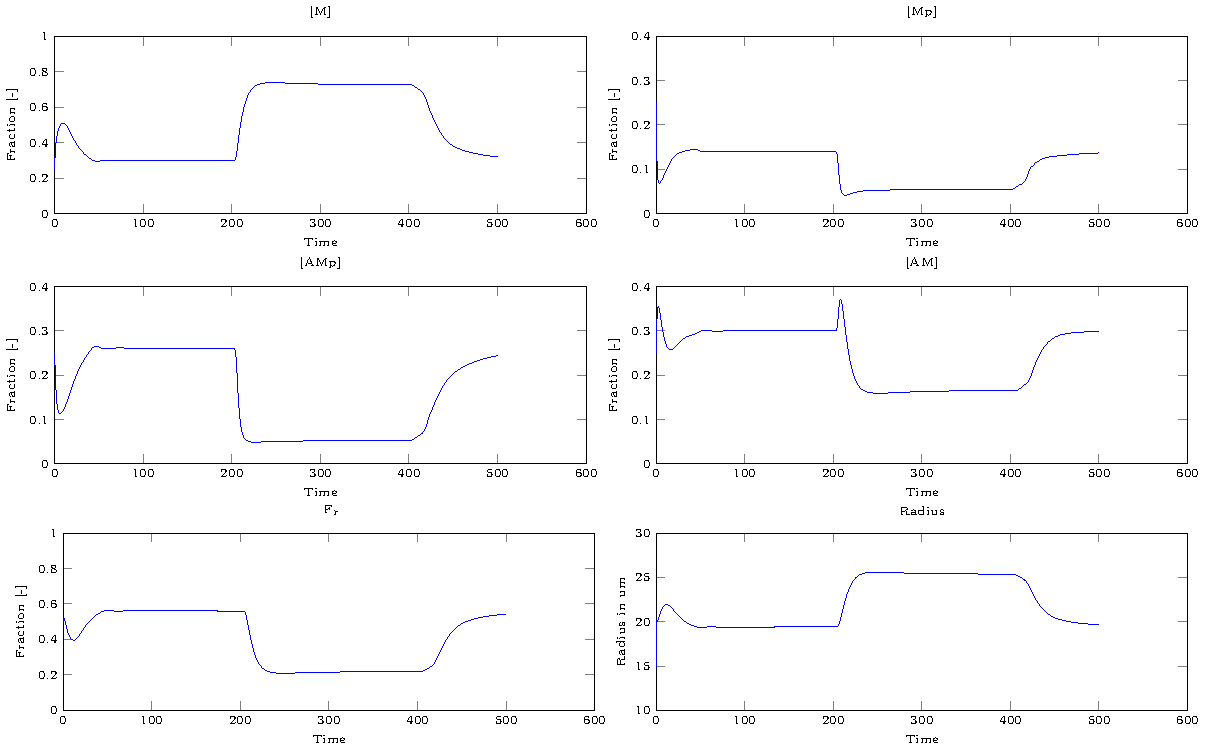
\includegraphics{figures/5_MC_model.pdf}
			\caption{The Myosin Contraction model}
			\label{fig:5MCm}
		\end{figure}
		
		\begin{figure}[h!]
			\centering
			\tiny 
			\setlength\figureheight{3 cm} 
			\setlength\figurewidth{9 cm}
			%% % This file was created by matlab2tikz v0.3.3.
% Copyright (c) 2008--2013, Nico Schlömer <nico.schloemer@gmail.com>
% All rights reserved.
% 
% The latest updates can be retrieved from
%   http://www.mathworks.com/matlabcentral/fileexchange/22022-matlab2tikz
% where you can also make suggestions and rate matlab2tikz.
% 
% 
% 
\begin{tikzpicture}

\begin{axis}[%
width=\figurewidth,
height=\figureheight,
scale only axis,
xmin=0,
xmax=600,
xlabel={Time [s]},
ymin=0,
ymax=20,
ylabel={$\text{[K}^\text{+}\text{]}_\text{s}\text{ [mM]}$},
name=plot3,
title={$\text{[K}^\text{+}\text{] in perivascular space}$}
]
\addplot [
color=blue,
solid,
forget plot
]
table[row sep=crcr]{
0 3\\
0.0011996 3.0002\\
0.0023992 3.0003\\
0.0035988 3.0004\\
0.0085566 3.001\\
0.013514 3.0015\\
0.018472 3.002\\
0.02343 3.0025\\
0.033542 3.0033\\
0.043655 3.004\\
0.053767 3.0046\\
0.063879 3.0052\\
0.073991 3.0056\\
0.084819 3.0061\\
0.095647 3.0065\\
0.10647 3.0068\\
0.1173 3.0071\\
0.12813 3.0074\\
0.14659 3.0079\\
0.16505 3.0083\\
0.18351 3.0086\\
0.20197 3.009\\
0.22042 3.0093\\
0.26398 3.0099\\
0.30753 3.0106\\
0.35108 3.0111\\
0.37397 3.0114\\
0.38969 3.0116\\
0.4054 3.0118\\
0.42111 3.012\\
0.43393 3.0121\\
0.44676 3.0123\\
0.45959 3.0124\\
0.47242 3.0125\\
0.48525 3.0127\\
0.50035 3.0129\\
0.51544 3.013\\
0.53054 3.0132\\
0.54564 3.0134\\
0.56073 3.0135\\
0.57728 3.0137\\
0.59382 3.0139\\
0.61036 3.0141\\
0.6269 3.0143\\
0.64344 3.0144\\
0.65998 3.0146\\
0.69992 3.0151\\
0.73986 3.0155\\
0.77979 3.016\\
0.81973 3.0164\\
0.85967 3.0168\\
0.99616 3.0184\\
1.1327 3.0199\\
1.2692 3.0214\\
1.4056 3.0229\\
1.6062 3.0251\\
1.8067 3.0273\\
2.0072 3.0296\\
2.2078 3.0318\\
2.4083 3.034\\
2.8551 3.0388\\
3.302 3.0436\\
3.7488 3.0484\\
4.1956 3.0531\\
4.6425 3.0578\\
5.3586 3.0651\\
6.0748 3.0724\\
6.791 3.0796\\
7.5072 3.0866\\
8.2234 3.0936\\
9.2234 3.1032\\
10.223 3.1126\\
11.223 3.1218\\
12.223 3.1309\\
12.523 3.1336\\
12.823 3.1362\\
13.123 3.1389\\
13.423 3.1416\\
13.513 3.1424\\
13.603 3.1431\\
13.693 3.1439\\
13.783 3.1447\\
13.873 3.1455\\
13.929 3.146\\
13.948 3.1462\\
13.967 3.1463\\
13.986 3.1465\\
14.004 3.1466\\
14.023 3.1468\\
14.079 3.1473\\
14.134 3.1478\\
14.189 3.1483\\
14.244 3.1488\\
14.299 3.1493\\
14.354 3.1497\\
14.409 3.1501\\
14.465 3.1506\\
14.52 3.151\\
14.575 3.1516\\
14.631 3.1522\\
14.686 3.153\\
14.742 3.1538\\
14.811 3.1551\\
14.88 3.1564\\
14.95 3.1578\\
15.019 3.1593\\
15.089 3.1608\\
15.202 3.1632\\
15.315 3.1654\\
15.428 3.1675\\
15.541 3.1694\\
15.654 3.1711\\
15.804 3.1732\\
15.954 3.1751\\
16.104 3.1769\\
16.255 3.1785\\
16.405 3.1801\\
16.675 3.1831\\
16.946 3.1861\\
17.216 3.1891\\
17.487 3.1919\\
17.757 3.1945\\
18.061 3.1973\\
18.364 3.1999\\
18.667 3.2024\\
18.971 3.2049\\
19.274 3.2073\\
19.375 3.2081\\
19.476 3.2089\\
19.576 3.2097\\
19.677 3.2105\\
19.778 3.2112\\
19.938 3.2125\\
20.097 3.2137\\
20.257 3.215\\
20.416 3.2162\\
20.576 3.2174\\
20.994 3.2207\\
21.411 3.2239\\
21.828 3.2271\\
22.056 3.2288\\
22.119 3.2293\\
22.183 3.2298\\
22.247 3.2303\\
22.31 3.2308\\
22.432 3.2317\\
22.554 3.2326\\
22.676 3.2336\\
22.798 3.2345\\
22.92 3.2355\\
23.367 3.239\\
23.684 3.2415\\
24 3.244\\
24.242 3.246\\
24.484 3.248\\
24.726 3.25\\
24.968 3.252\\
25.298 3.2547\\
25.628 3.2574\\
25.958 3.2602\\
26.288 3.2629\\
26.618 3.2656\\
27.087 3.2693\\
27.556 3.273\\
28.025 3.2767\\
28.494 3.2803\\
28.964 3.2839\\
29.615 3.2888\\
30.266 3.2936\\
30.917 3.2984\\
31.569 3.3032\\
32.372 3.309\\
33.175 3.3148\\
33.979 3.3206\\
34.782 3.3263\\
35.586 3.332\\
36.23 3.3365\\
36.875 3.3409\\
37.52 3.3453\\
38.164 3.3497\\
38.969 3.3551\\
39.774 3.3604\\
40.579 3.3656\\
41.384 3.3708\\
42.189 3.3759\\
43.189 3.3821\\
44.189 3.3882\\
45.189 3.3942\\
46.189 3.4001\\
47.189 3.4058\\
48.189 3.4114\\
49.189 3.4168\\
50.189 3.422\\
51.189 3.4271\\
52.189 3.4321\\
53.189 3.4369\\
54.189 3.4417\\
55.189 3.4463\\
56.189 3.4507\\
57.189 3.4551\\
58.189 3.4594\\
59.189 3.4636\\
60.189 3.4677\\
61.189 3.4718\\
62.189 3.4757\\
63.189 3.4796\\
64.189 3.4834\\
65.189 3.4871\\
66.189 3.4907\\
67.189 3.4943\\
68.189 3.4978\\
69.189 3.5011\\
70.189 3.5045\\
71.189 3.5077\\
72.189 3.5109\\
73.189 3.514\\
74.189 3.5171\\
75.189 3.5201\\
76.189 3.523\\
77.189 3.5258\\
78.189 3.5286\\
79.189 3.5313\\
80.189 3.5339\\
81.189 3.5365\\
82.189 3.5391\\
83.189 3.5416\\
84.189 3.544\\
85.189 3.5464\\
86.189 3.5487\\
87.189 3.551\\
88.189 3.5532\\
89.189 3.5554\\
90.189 3.5575\\
91.189 3.5596\\
92.189 3.5616\\
93.189 3.5636\\
94.189 3.5656\\
95.189 3.5675\\
96.189 3.5693\\
97.189 3.5712\\
98.189 3.573\\
99.189 3.5747\\
100.19 3.5764\\
101.19 3.5781\\
102.19 3.5797\\
103.19 3.5814\\
104.19 3.5829\\
105.19 3.5845\\
106.19 3.586\\
107.19 3.5874\\
108.19 3.5889\\
109.19 3.5903\\
110.19 3.5917\\
111.19 3.593\\
112.19 3.5944\\
113.19 3.5956\\
114.19 3.5969\\
115.19 3.5982\\
116.19 3.5994\\
117.19 3.6006\\
118.19 3.6017\\
119.19 3.6029\\
120.19 3.604\\
121.19 3.6051\\
122.19 3.6061\\
123.19 3.6072\\
124.19 3.6082\\
125.19 3.6092\\
126.19 3.6102\\
127.19 3.6111\\
128.19 3.6121\\
129.19 3.613\\
130.19 3.6139\\
131.19 3.6148\\
132.19 3.6156\\
133.19 3.6165\\
134.19 3.6173\\
135.19 3.6181\\
136.19 3.6189\\
137.19 3.6197\\
138.19 3.6205\\
139.19 3.6212\\
140.19 3.6219\\
141.19 3.6226\\
142.19 3.6233\\
143.19 3.624\\
144.19 3.6247\\
145.19 3.6253\\
146.19 3.626\\
147.19 3.6266\\
148.19 3.6272\\
149.19 3.6278\\
150.19 3.6284\\
151.19 3.629\\
152.19 3.6295\\
153.19 3.6301\\
154.19 3.6306\\
155.19 3.6312\\
156.19 3.6317\\
157.19 3.6322\\
158.19 3.6327\\
159.19 3.6332\\
160.19 3.6336\\
161.19 3.6341\\
162.19 3.6346\\
163.19 3.635\\
164.19 3.6354\\
165.19 3.6359\\
166.19 3.6363\\
167.19 3.6367\\
168.19 3.6371\\
169.19 3.6375\\
170.19 3.6379\\
171.19 3.6383\\
172.19 3.6386\\
173.19 3.639\\
174.19 3.6393\\
175.19 3.6397\\
176.19 3.64\\
177.19 3.6404\\
178.19 3.6407\\
179.19 3.641\\
180.19 3.6413\\
181.19 3.6416\\
182.19 3.6419\\
183.19 3.6422\\
184.19 3.6425\\
185.19 3.6428\\
186.19 3.643\\
187.19 3.6433\\
188.19 3.6436\\
189.19 3.6438\\
190.19 3.6441\\
191.19 3.6443\\
192.19 3.6446\\
193.19 3.6448\\
194.19 3.645\\
195.19 3.6453\\
196.19 3.6455\\
196.81 3.6456\\
197.25 3.6457\\
197.57 3.6458\\
197.82 3.6458\\
198.03 3.6459\\
198.24 3.6459\\
198.38 3.6459\\
198.52 3.646\\
198.63 3.646\\
198.74 3.646\\
198.83 3.646\\
198.92 3.646\\
199.01 3.646\\
199.17 3.646\\
199.32 3.646\\
199.47 3.646\\
199.62 3.646\\
199.84 3.646\\
200.07 3.6457\\
200.29 3.6457\\
200.51 3.6471\\
200.69 3.6503\\
200.87 3.6559\\
201.05 3.6652\\
201.23 3.6798\\
201.42 3.7023\\
201.6 3.7364\\
201.79 3.7857\\
201.97 3.8557\\
202.15 3.9532\\
202.34 4.0856\\
202.63 4.3805\\
202.92 4.7972\\
203.21 5.3395\\
203.5 5.9916\\
203.79 6.7189\\
204.09 7.5047\\
204.39 8.2733\\
204.69 8.9844\\
204.94 9.5062\\
205.19 9.9615\\
205.44 10.344\\
205.68 10.654\\
205.85 10.825\\
206.02 10.965\\
206.19 11.079\\
206.36 11.167\\
206.6 11.257\\
206.84 11.312\\
207.08 11.338\\
207.32 11.341\\
207.65 11.319\\
207.99 11.276\\
208.32 11.219\\
208.65 11.155\\
208.99 11.088\\
209.66 10.948\\
210.18 10.845\\
210.7 10.747\\
211.22 10.655\\
211.74 10.568\\
212.26 10.488\\
212.9 10.396\\
213.54 10.311\\
214.18 10.235\\
214.82 10.167\\
215.46 10.106\\
216.16 10.048\\
216.87 9.9977\\
217.57 9.9541\\
218.27 9.9159\\
218.98 9.882\\
219.98 9.8399\\
220.98 9.8039\\
221.98 9.774\\
222.98 9.7505\\
223.98 9.7327\\
224.98 9.7185\\
225.98 9.7066\\
226.98 9.6962\\
227.98 9.687\\
228.98 9.6793\\
229.98 9.6733\\
230.98 9.6687\\
231.98 9.665\\
232.98 9.6619\\
233.98 9.659\\
234.98 9.6565\\
235.98 9.6547\\
236.98 9.6528\\
237.98 9.6519\\
238.98 9.651\\
239.98 9.6502\\
240.98 9.6495\\
241.98 9.649\\
242.98 9.6484\\
243.98 9.648\\
244.98 9.6476\\
245.98 9.6473\\
246.98 9.6471\\
247.98 9.6469\\
248.98 9.6467\\
249.98 9.6466\\
250.98 9.6465\\
251.98 9.6464\\
252.98 9.6464\\
253.98 9.6463\\
254.98 9.6462\\
255.98 9.6462\\
256.98 9.6462\\
257.98 9.6461\\
258.98 9.6461\\
259.98 9.6461\\
260.98 9.6461\\
261.98 9.6461\\
262.98 9.6461\\
263.98 9.646\\
264.98 9.646\\
265.98 9.646\\
266.98 9.646\\
267.98 9.646\\
268.98 9.646\\
269.98 9.646\\
270.98 9.646\\
271.98 9.646\\
272.98 9.646\\
273.98 9.646\\
274.98 9.646\\
275.98 9.646\\
276.98 9.646\\
277.98 9.646\\
278.98 9.646\\
279.98 9.646\\
280.98 9.646\\
281.98 9.646\\
282.98 9.646\\
283.98 9.646\\
284.98 9.646\\
285.98 9.646\\
286.98 9.646\\
287.98 9.646\\
288.98 9.646\\
289.98 9.646\\
290.98 9.646\\
291.98 9.646\\
292.98 9.646\\
293.98 9.646\\
294.98 9.646\\
295.98 9.646\\
296.98 9.646\\
297.98 9.646\\
298.98 9.646\\
299.98 9.646\\
300.98 9.646\\
301.98 9.646\\
302.98 9.646\\
303.98 9.646\\
304.98 9.646\\
305.98 9.646\\
306.98 9.646\\
307.98 9.646\\
308.98 9.646\\
309.98 9.646\\
310.98 9.646\\
311.98 9.646\\
312.98 9.646\\
313.98 9.6459\\
314.98 9.6459\\
315.98 9.6459\\
316.98 9.6459\\
317.98 9.6459\\
318.98 9.6459\\
319.98 9.6459\\
320.98 9.6459\\
321.98 9.6459\\
322.98 9.6459\\
323.98 9.6459\\
324.98 9.6459\\
325.98 9.6459\\
326.98 9.6459\\
327.98 9.6459\\
328.98 9.6459\\
329.98 9.6459\\
330.98 9.6459\\
331.98 9.6459\\
332.98 9.6459\\
333.98 9.6459\\
334.98 9.6459\\
335.98 9.6459\\
336.98 9.6459\\
337.98 9.6459\\
338.98 9.6459\\
339.98 9.6459\\
340.98 9.6459\\
341.98 9.6459\\
342.98 9.6459\\
343.98 9.6459\\
344.98 9.6459\\
345.98 9.6459\\
346.98 9.6459\\
347.98 9.6459\\
348.98 9.6459\\
349.98 9.6459\\
350.98 9.6459\\
351.98 9.6459\\
352.98 9.6459\\
353.98 9.6459\\
354.98 9.6459\\
355.98 9.6459\\
356.98 9.6459\\
357.98 9.6459\\
358.98 9.6459\\
359.98 9.6459\\
360.98 9.6459\\
361.98 9.6459\\
362.98 9.6459\\
363.98 9.6459\\
364.98 9.6459\\
365.98 9.6459\\
366.98 9.6459\\
367.98 9.6459\\
368.98 9.6459\\
369.98 9.6459\\
370.98 9.6459\\
371.98 9.6459\\
372.98 9.6459\\
373.98 9.6459\\
374.98 9.6459\\
375.98 9.6459\\
376.98 9.6459\\
377.98 9.6459\\
378.98 9.6459\\
379.98 9.6459\\
380.98 9.6459\\
381.98 9.6459\\
382.98 9.6459\\
383.98 9.6459\\
384.98 9.6459\\
385.98 9.6459\\
386.98 9.6459\\
387.98 9.6459\\
388.98 9.6459\\
389.98 9.6459\\
390.98 9.6459\\
391.98 9.6459\\
392.98 9.6459\\
393.98 9.6459\\
394.98 9.6459\\
395.98 9.6459\\
396.98 9.6459\\
397.98 9.6461\\
398.44 9.6461\\
398.8 9.6462\\
399.07 9.6462\\
399.35 9.6462\\
399.55 9.6462\\
399.76 9.6461\\
399.96 9.6461\\
400.26 9.6208\\
400.34 9.6069\\
400.43 9.5914\\
400.52 9.5753\\
400.61 9.5593\\
400.92 9.5046\\
401.24 9.453\\
401.56 9.4044\\
401.87 9.3594\\
402.11 9.328\\
402.35 9.299\\
402.59 9.2724\\
402.83 9.248\\
403.14 9.2193\\
403.45 9.1935\\
403.77 9.1705\\
404.08 9.1498\\
404.39 9.1312\\
404.93 9.103\\
405.47 9.079\\
406.02 9.0583\\
406.56 9.0409\\
407.1 9.0273\\
408.1 9.0087\\
408.77 9.0006\\
409.43 8.9956\\
410.1 8.9861\\
410.61 8.972\\
411.12 8.954\\
411.63 8.9349\\
412.15 8.9149\\
412.66 8.8942\\
413.31 8.8678\\
413.95 8.8412\\
414.6 8.8141\\
415.25 8.7863\\
415.9 8.7578\\
416.77 8.7178\\
417.65 8.6763\\
418.52 8.6332\\
419.4 8.5888\\
420.28 8.5436\\
421.2 8.4959\\
422.12 8.4486\\
423.04 8.402\\
423.96 8.3558\\
424.89 8.3094\\
425.81 8.2626\\
426.73 8.2156\\
427.68 8.1671\\
428.64 8.1187\\
429.59 8.0706\\
430.55 8.0225\\
431.5 7.9745\\
432.5 7.9243\\
433.5 7.8744\\
434.5 7.8247\\
435.5 7.7751\\
436.5 7.7256\\
437.5 7.6763\\
438.5 7.6271\\
439.5 7.5782\\
440.5 7.5295\\
441.5 7.4809\\
442.5 7.4326\\
443.5 7.3845\\
444.5 7.3367\\
445.5 7.289\\
446.5 7.2416\\
447.5 7.1945\\
448.5 7.1475\\
449.5 7.1008\\
450.5 7.0544\\
451.5 7.0082\\
452.5 6.9623\\
453.5 6.9167\\
454.5 6.8714\\
455.5 6.8265\\
456.5 6.7818\\
457.5 6.7375\\
458.5 6.6935\\
459.5 6.6499\\
460.5 6.6066\\
461.5 6.5637\\
462.5 6.5212\\
463.5 6.479\\
464.5 6.4373\\
465.5 6.3959\\
466.5 6.3549\\
467.5 6.3143\\
468.5 6.2741\\
469.5 6.2343\\
470.5 6.1949\\
471.5 6.1559\\
472.5 6.1174\\
473.5 6.0792\\
474.5 6.0415\\
475.5 6.0042\\
476.5 5.9673\\
477.5 5.9309\\
478.5 5.8949\\
479.5 5.8593\\
480.5 5.8241\\
481.5 5.7893\\
482.5 5.755\\
483.5 5.7212\\
484.5 5.6877\\
485.5 5.6547\\
486.5 5.6221\\
487.5 5.5899\\
488.5 5.5582\\
489.5 5.5268\\
490.5 5.4959\\
491.5 5.4655\\
492.5 5.4354\\
493.5 5.4058\\
494.5 5.3766\\
495.5 5.3478\\
496.5 5.3194\\
497.5 5.2915\\
498.5 5.2639\\
499.5 5.2367\\
500 5.2234\\
};
\end{axis}

\begin{axis}[%
width=\figurewidth,
height=\figureheight,
scale only axis,
xmin=0,
xmax=600,
xlabel={Time [s]},
ymin=0,
ymax=20,
ylabel={$\text{[K}^\text{+}\text{]}_\text{s}\text{ [mM]}$},
name=plot1,
at=(plot3.above north west),
anchor=below south west,
title={$\text{[K}^\text{+}\text{] in synaptic cleft}$}
]
\addplot [
color=blue,
solid,
forget plot
]
table[row sep=crcr]{
0 3\\
0.0011996 2.9989\\
0.0023992 3.0006\\
0.0035988 3.0019\\
0.0085566 3.007\\
0.013514 3.0116\\
0.018472 3.0159\\
0.02343 3.0198\\
0.033542 3.0268\\
0.043655 3.0326\\
0.053767 3.0375\\
0.063879 3.0416\\
0.073991 3.045\\
0.084819 3.048\\
0.095647 3.0505\\
0.10647 3.0525\\
0.1173 3.0542\\
0.12813 3.0556\\
0.14659 3.0574\\
0.16505 3.0587\\
0.18351 3.0596\\
0.20197 3.0603\\
0.22042 3.0607\\
0.26398 3.0612\\
0.30753 3.0614\\
0.35108 3.0613\\
0.37397 3.0613\\
0.38969 3.0612\\
0.4054 3.0612\\
0.42111 3.0611\\
0.43393 3.0611\\
0.44676 3.061\\
0.45959 3.0609\\
0.47242 3.0609\\
0.48525 3.0608\\
0.50035 3.0608\\
0.51544 3.0607\\
0.53054 3.0606\\
0.54564 3.0605\\
0.56073 3.0605\\
0.57728 3.0604\\
0.59382 3.0603\\
0.61036 3.0602\\
0.6269 3.0601\\
0.64344 3.06\\
0.65998 3.0599\\
0.69992 3.0597\\
0.73986 3.0595\\
0.77979 3.0593\\
0.81973 3.0591\\
0.85967 3.0589\\
0.99616 3.0583\\
1.1327 3.0577\\
1.2692 3.0571\\
1.4056 3.0566\\
1.6062 3.0559\\
1.8067 3.0553\\
2.0072 3.0548\\
2.2078 3.0543\\
2.4083 3.0539\\
2.8551 3.0533\\
3.302 3.0528\\
3.7488 3.0524\\
4.1956 3.0522\\
4.6425 3.052\\
5.3586 3.0518\\
6.0748 3.0517\\
6.791 3.0516\\
7.5072 3.0516\\
8.2234 3.0515\\
9.2234 3.0515\\
10.223 3.0515\\
11.223 3.0515\\
12.223 3.0515\\
12.523 3.0515\\
12.823 3.0515\\
13.123 3.0515\\
13.423 3.0515\\
13.513 3.0515\\
13.603 3.0515\\
13.693 3.0515\\
13.783 3.0515\\
13.873 3.0515\\
13.929 3.0515\\
13.948 3.0515\\
13.967 3.0515\\
13.986 3.0515\\
14.004 3.0515\\
14.023 3.0515\\
14.079 3.0515\\
14.134 3.0515\\
14.189 3.0515\\
14.244 3.0515\\
14.299 3.0515\\
14.354 3.0515\\
14.409 3.0515\\
14.465 3.0515\\
14.52 3.0515\\
14.575 3.0515\\
14.631 3.0515\\
14.686 3.0515\\
14.742 3.0515\\
14.811 3.0515\\
14.88 3.0515\\
14.95 3.0515\\
15.019 3.0515\\
15.089 3.0515\\
15.202 3.0515\\
15.315 3.0515\\
15.428 3.0515\\
15.541 3.0515\\
15.654 3.0515\\
15.804 3.0515\\
15.954 3.0515\\
16.104 3.0515\\
16.255 3.0515\\
16.405 3.0515\\
16.675 3.0515\\
16.946 3.0515\\
17.216 3.0515\\
17.487 3.0515\\
17.757 3.0515\\
18.061 3.0515\\
18.364 3.0515\\
18.667 3.0515\\
18.971 3.0515\\
19.274 3.0515\\
19.375 3.0515\\
19.476 3.0515\\
19.576 3.0515\\
19.677 3.0515\\
19.778 3.0515\\
19.938 3.0515\\
20.097 3.0515\\
20.257 3.0515\\
20.416 3.0515\\
20.576 3.0515\\
20.994 3.0515\\
21.411 3.0515\\
21.828 3.0515\\
22.056 3.0515\\
22.119 3.0515\\
22.183 3.0515\\
22.247 3.0515\\
22.31 3.0515\\
22.432 3.0515\\
22.554 3.0515\\
22.676 3.0515\\
22.798 3.0515\\
22.92 3.0515\\
23.367 3.0515\\
23.684 3.0515\\
24 3.0515\\
24.242 3.0515\\
24.484 3.0515\\
24.726 3.0515\\
24.968 3.0515\\
25.298 3.0515\\
25.628 3.0515\\
25.958 3.0515\\
26.288 3.0515\\
26.618 3.0515\\
27.087 3.0515\\
27.556 3.0515\\
28.025 3.0515\\
28.494 3.0515\\
28.964 3.0515\\
29.615 3.0515\\
30.266 3.0515\\
30.917 3.0515\\
31.569 3.0515\\
32.372 3.0515\\
33.175 3.0515\\
33.979 3.0515\\
34.782 3.0515\\
35.586 3.0515\\
36.23 3.0515\\
36.875 3.0515\\
37.52 3.0515\\
38.164 3.0515\\
38.969 3.0515\\
39.774 3.0515\\
40.579 3.0515\\
41.384 3.0515\\
42.189 3.0515\\
43.189 3.0515\\
44.189 3.0515\\
45.189 3.0515\\
46.189 3.0515\\
47.189 3.0515\\
48.189 3.0515\\
49.189 3.0515\\
50.189 3.0515\\
51.189 3.0515\\
52.189 3.0515\\
53.189 3.0515\\
54.189 3.0515\\
55.189 3.0515\\
56.189 3.0515\\
57.189 3.0515\\
58.189 3.0515\\
59.189 3.0515\\
60.189 3.0515\\
61.189 3.0515\\
62.189 3.0515\\
63.189 3.0515\\
64.189 3.0515\\
65.189 3.0515\\
66.189 3.0515\\
67.189 3.0515\\
68.189 3.0515\\
69.189 3.0515\\
70.189 3.0515\\
71.189 3.0515\\
72.189 3.0515\\
73.189 3.0515\\
74.189 3.0515\\
75.189 3.0515\\
76.189 3.0515\\
77.189 3.0515\\
78.189 3.0515\\
79.189 3.0515\\
80.189 3.0515\\
81.189 3.0515\\
82.189 3.0515\\
83.189 3.0515\\
84.189 3.0515\\
85.189 3.0515\\
86.189 3.0515\\
87.189 3.0515\\
88.189 3.0515\\
89.189 3.0515\\
90.189 3.0515\\
91.189 3.0515\\
92.189 3.0515\\
93.189 3.0515\\
94.189 3.0515\\
95.189 3.0515\\
96.189 3.0515\\
97.189 3.0515\\
98.189 3.0515\\
99.189 3.0515\\
100.19 3.0515\\
101.19 3.0515\\
102.19 3.0515\\
103.19 3.0515\\
104.19 3.0515\\
105.19 3.0515\\
106.19 3.0515\\
107.19 3.0515\\
108.19 3.0515\\
109.19 3.0515\\
110.19 3.0515\\
111.19 3.0515\\
112.19 3.0515\\
113.19 3.0515\\
114.19 3.0515\\
115.19 3.0515\\
116.19 3.0515\\
117.19 3.0515\\
118.19 3.0515\\
119.19 3.0515\\
120.19 3.0515\\
121.19 3.0515\\
122.19 3.0515\\
123.19 3.0515\\
124.19 3.0515\\
125.19 3.0515\\
126.19 3.0515\\
127.19 3.0515\\
128.19 3.0515\\
129.19 3.0515\\
130.19 3.0515\\
131.19 3.0515\\
132.19 3.0515\\
133.19 3.0515\\
134.19 3.0515\\
135.19 3.0515\\
136.19 3.0515\\
137.19 3.0515\\
138.19 3.0515\\
139.19 3.0515\\
140.19 3.0515\\
141.19 3.0515\\
142.19 3.0515\\
143.19 3.0515\\
144.19 3.0515\\
145.19 3.0515\\
146.19 3.0515\\
147.19 3.0515\\
148.19 3.0515\\
149.19 3.0515\\
150.19 3.0515\\
151.19 3.0515\\
152.19 3.0515\\
153.19 3.0515\\
154.19 3.0515\\
155.19 3.0515\\
156.19 3.0515\\
157.19 3.0515\\
158.19 3.0515\\
159.19 3.0515\\
160.19 3.0515\\
161.19 3.0515\\
162.19 3.0515\\
163.19 3.0515\\
164.19 3.0515\\
165.19 3.0515\\
166.19 3.0515\\
167.19 3.0515\\
168.19 3.0515\\
169.19 3.0515\\
170.19 3.0515\\
171.19 3.0515\\
172.19 3.0515\\
173.19 3.0515\\
174.19 3.0515\\
175.19 3.0515\\
176.19 3.0515\\
177.19 3.0515\\
178.19 3.0515\\
179.19 3.0515\\
180.19 3.0515\\
181.19 3.0515\\
182.19 3.0515\\
183.19 3.0515\\
184.19 3.0515\\
185.19 3.0515\\
186.19 3.0515\\
187.19 3.0515\\
188.19 3.0515\\
189.19 3.0515\\
190.19 3.0515\\
191.19 3.0515\\
192.19 3.0515\\
193.19 3.0515\\
194.19 3.0515\\
195.19 3.0515\\
196.19 3.0515\\
196.81 3.0515\\
197.25 3.0515\\
197.57 3.0515\\
197.82 3.0515\\
198.03 3.0515\\
198.24 3.0515\\
198.38 3.0515\\
198.52 3.0515\\
198.63 3.0515\\
198.74 3.0515\\
198.83 3.0515\\
198.92 3.0515\\
199.01 3.0515\\
199.17 3.0515\\
199.32 3.0515\\
199.47 3.0515\\
199.62 3.0515\\
199.84 3.0515\\
200.07 2.9912\\
200.29 3.1156\\
200.51 3.3942\\
200.69 3.6496\\
200.87 3.9074\\
201.05 4.1902\\
201.23 4.5078\\
201.42 4.8538\\
201.6 5.2296\\
201.79 5.6317\\
201.97 6.0627\\
202.15 6.5202\\
202.34 6.9979\\
202.63 7.7743\\
202.92 8.5568\\
203.21 9.3133\\
203.5 10.007\\
203.79 10.604\\
204.09 11.094\\
204.39 11.441\\
204.69 11.644\\
204.94 11.711\\
205.19 11.691\\
205.44 11.596\\
205.68 11.442\\
205.85 11.31\\
206.02 11.161\\
206.19 11.001\\
206.36 10.834\\
206.6 10.59\\
206.84 10.347\\
207.08 10.112\\
207.32 9.8905\\
207.65 9.612\\
207.99 9.3706\\
208.32 9.1671\\
208.65 8.9996\\
208.99 8.8638\\
209.66 8.6659\\
210.18 8.565\\
210.7 8.4926\\
211.22 8.44\\
211.74 8.4018\\
212.26 8.374\\
212.9 8.3496\\
213.54 8.3327\\
214.18 8.3213\\
214.82 8.3136\\
215.46 8.3083\\
216.16 8.3043\\
216.87 8.3017\\
217.57 8.3\\
218.27 8.2989\\
218.98 8.2982\\
219.98 8.2975\\
220.98 8.2971\\
221.98 8.2969\\
222.98 8.2968\\
223.98 8.2967\\
224.98 8.2967\\
225.98 8.2967\\
226.98 8.2967\\
227.98 8.2967\\
228.98 8.2967\\
229.98 8.2967\\
230.98 8.2967\\
231.98 8.2967\\
232.98 8.2967\\
233.98 8.2967\\
234.98 8.2967\\
235.98 8.2967\\
236.98 8.2967\\
237.98 8.2967\\
238.98 8.2967\\
239.98 8.2967\\
240.98 8.2967\\
241.98 8.2967\\
242.98 8.2967\\
243.98 8.2967\\
244.98 8.2967\\
245.98 8.2967\\
246.98 8.2967\\
247.98 8.2967\\
248.98 8.2967\\
249.98 8.2967\\
250.98 8.2967\\
251.98 8.2967\\
252.98 8.2967\\
253.98 8.2967\\
254.98 8.2967\\
255.98 8.2967\\
256.98 8.2967\\
257.98 8.2967\\
258.98 8.2967\\
259.98 8.2967\\
260.98 8.2967\\
261.98 8.2967\\
262.98 8.2967\\
263.98 8.2967\\
264.98 8.2967\\
265.98 8.2967\\
266.98 8.2967\\
267.98 8.2967\\
268.98 8.2967\\
269.98 8.2967\\
270.98 8.2967\\
271.98 8.2967\\
272.98 8.2967\\
273.98 8.2967\\
274.98 8.2967\\
275.98 8.2967\\
276.98 8.2967\\
277.98 8.2967\\
278.98 8.2967\\
279.98 8.2967\\
280.98 8.2967\\
281.98 8.2967\\
282.98 8.2967\\
283.98 8.2967\\
284.98 8.2967\\
285.98 8.2967\\
286.98 8.2967\\
287.98 8.2967\\
288.98 8.2967\\
289.98 8.2967\\
290.98 8.2967\\
291.98 8.2967\\
292.98 8.2967\\
293.98 8.2967\\
294.98 8.2967\\
295.98 8.2967\\
296.98 8.2967\\
297.98 8.2967\\
298.98 8.2967\\
299.98 8.2967\\
300.98 8.2967\\
301.98 8.2967\\
302.98 8.2967\\
303.98 8.2967\\
304.98 8.2967\\
305.98 8.2967\\
306.98 8.2967\\
307.98 8.2967\\
308.98 8.2967\\
309.98 8.2967\\
310.98 8.2967\\
311.98 8.2967\\
312.98 8.2967\\
313.98 8.2967\\
314.98 8.2967\\
315.98 8.2967\\
316.98 8.2967\\
317.98 8.2967\\
318.98 8.2967\\
319.98 8.2967\\
320.98 8.2967\\
321.98 8.2967\\
322.98 8.2967\\
323.98 8.2967\\
324.98 8.2967\\
325.98 8.2967\\
326.98 8.2967\\
327.98 8.2967\\
328.98 8.2967\\
329.98 8.2967\\
330.98 8.2967\\
331.98 8.2967\\
332.98 8.2967\\
333.98 8.2967\\
334.98 8.2967\\
335.98 8.2967\\
336.98 8.2967\\
337.98 8.2967\\
338.98 8.2967\\
339.98 8.2967\\
340.98 8.2967\\
341.98 8.2967\\
342.98 8.2967\\
343.98 8.2967\\
344.98 8.2967\\
345.98 8.2967\\
346.98 8.2967\\
347.98 8.2967\\
348.98 8.2967\\
349.98 8.2967\\
350.98 8.2967\\
351.98 8.2967\\
352.98 8.2967\\
353.98 8.2967\\
354.98 8.2967\\
355.98 8.2967\\
356.98 8.2967\\
357.98 8.2967\\
358.98 8.2967\\
359.98 8.2967\\
360.98 8.2967\\
361.98 8.2967\\
362.98 8.2967\\
363.98 8.2967\\
364.98 8.2967\\
365.98 8.2967\\
366.98 8.2967\\
367.98 8.2967\\
368.98 8.2967\\
369.98 8.2967\\
370.98 8.2967\\
371.98 8.2967\\
372.98 8.2967\\
373.98 8.2967\\
374.98 8.2967\\
375.98 8.2967\\
376.98 8.2967\\
377.98 8.2967\\
378.98 8.2967\\
379.98 8.2967\\
380.98 8.2967\\
381.98 8.2967\\
382.98 8.2967\\
383.98 8.2967\\
384.98 8.2967\\
385.98 8.2967\\
386.98 8.2967\\
387.98 8.2967\\
388.98 8.2967\\
389.98 8.2967\\
390.98 8.2967\\
391.98 8.2967\\
392.98 8.2967\\
393.98 8.2967\\
394.98 8.2967\\
395.98 8.2967\\
396.98 8.2967\\
397.98 8.2967\\
398.44 8.2967\\
398.8 8.2967\\
399.07 8.2967\\
399.35 8.2967\\
399.55 8.2967\\
399.76 8.2967\\
399.96 8.2967\\
400.26 7.3905\\
400.34 7.0622\\
400.43 6.8208\\
400.52 6.6438\\
400.61 6.5023\\
400.92 6.0915\\
401.24 5.7767\\
401.56 5.5044\\
401.87 5.2659\\
402.11 5.1045\\
402.35 4.9572\\
402.59 4.821\\
402.83 4.6938\\
403.14 4.5403\\
403.45 4.3973\\
403.77 4.263\\
404.08 4.1358\\
404.39 4.0147\\
404.93 3.8147\\
405.47 3.6265\\
406.02 3.4486\\
406.56 3.2805\\
407.1 3.1207\\
408.1 2.8448\\
408.77 2.6747\\
409.43 2.5157\\
410.1 2.8446\\
410.61 2.9864\\
411.12 3.0227\\
411.63 3.0713\\
412.15 3.1312\\
412.66 3.1434\\
413.31 3.1524\\
413.95 3.1686\\
414.6 3.1806\\
415.25 3.1855\\
415.9 3.1888\\
416.77 3.1921\\
417.65 3.1937\\
418.52 3.1944\\
419.4 3.1949\\
420.28 3.1952\\
421.2 3.1953\\
422.12 3.1953\\
423.04 3.1954\\
423.96 3.1954\\
424.89 3.1954\\
425.81 3.1954\\
426.73 3.1954\\
427.68 3.1954\\
428.64 3.1954\\
429.59 3.1954\\
430.55 3.1954\\
431.5 3.1954\\
432.5 3.1954\\
433.5 3.1954\\
434.5 3.1954\\
435.5 3.1954\\
436.5 3.1954\\
437.5 3.1954\\
438.5 3.1954\\
439.5 3.1954\\
440.5 3.1954\\
441.5 3.1954\\
442.5 3.1954\\
443.5 3.1954\\
444.5 3.1954\\
445.5 3.1954\\
446.5 3.1954\\
447.5 3.1954\\
448.5 3.1954\\
449.5 3.1954\\
450.5 3.1954\\
451.5 3.1954\\
452.5 3.1954\\
453.5 3.1954\\
454.5 3.1954\\
455.5 3.1954\\
456.5 3.1954\\
457.5 3.1954\\
458.5 3.1954\\
459.5 3.1954\\
460.5 3.1954\\
461.5 3.1954\\
462.5 3.1954\\
463.5 3.1954\\
464.5 3.1954\\
465.5 3.1954\\
466.5 3.1954\\
467.5 3.1954\\
468.5 3.1954\\
469.5 3.1954\\
470.5 3.1954\\
471.5 3.1954\\
472.5 3.1954\\
473.5 3.1954\\
474.5 3.1954\\
475.5 3.1954\\
476.5 3.1954\\
477.5 3.1954\\
478.5 3.1954\\
479.5 3.1954\\
480.5 3.1954\\
481.5 3.1954\\
482.5 3.1954\\
483.5 3.1954\\
484.5 3.1954\\
485.5 3.1954\\
486.5 3.1954\\
487.5 3.1954\\
488.5 3.1954\\
489.5 3.1954\\
490.5 3.1954\\
491.5 3.1954\\
492.5 3.1954\\
493.5 3.1954\\
494.5 3.1954\\
495.5 3.1954\\
496.5 3.1954\\
497.5 3.1954\\
498.5 3.1954\\
499.5 3.1954\\
500 3.1954\\
};
\end{axis}

\begin{axis}[%
width=\figurewidth,
height=\figureheight,
scale only axis,
xmin=0,
xmax=600,
xlabel={Time [s]},
ymin=-5,
ymax=5,
ylabel={$\text{K}^\text{+}\text{ flux [}\mu\text{M/s]}$},
name=plot2,
at=(plot1.right of south east),
anchor=left of south west,
title={$\text{K}^\text{+}\text{ flux through the BK channel}$}
]
\addplot [
color=blue,
solid,
forget plot
]
table[row sep=crcr]{
0 0.113285245901639\\
0.0011996 0.110367673587195\\
0.0023992 0.108143520112822\\
0.0035988 0.105901838277496\\
0.0085566 0.0970384703683054\\
0.013514 0.0889000032796563\\
0.018472 0.0814650224656456\\
0.02343 0.0746847482085171\\
0.033542 0.0627180899908173\\
0.043655 0.0529080921538083\\
0.053767 0.0448848077396081\\
0.063879 0.0383366674318696\\
0.073991 0.033011953367111\\
0.084819 0.0284187053190792\\
0.095647 0.0247548778488277\\
0.10647 0.0218376481776\\
0.1173 0.0195156741867786\\
0.12813 0.0176692407325431\\
0.14659 0.0153720796786622\\
0.16505 0.0138232015214112\\
0.18351 0.0127727138594708\\
0.20197 0.0120608196721311\\
0.22042 0.0115807937574794\\
0.26398 0.0110246701090075\\
0.30753 0.0107948137949121\\
0.35108 0.0106624926244018\\
0.37397 0.0106097061282022\\
0.38969 0.0105893729308028\\
0.4054 0.0105762517413751\\
0.42111 0.0105659171364888\\
0.43393 0.01055787731288\\
0.44676 0.0105503294109935\\
0.45959 0.0105434372900244\\
0.47242 0.0105372097215621\\
0.48525 0.0105309734513274\\
0.50035 0.0105240818734534\\
0.51544 0.0105173543967749\\
0.53054 0.0105107910132245\\
0.54564 0.0105045638529735\\
0.56073 0.0104980007865758\\
0.57728 0.0104911102007374\\
0.59382 0.0104840559761413\\
0.61036 0.010477001982729\\
0.6269 0.0104701197830469\\
0.64344 0.0104632299927902\\
0.65998 0.0104561765717937\\
0.69992 0.0104391211023906\\
0.73986 0.0104222375147464\\
0.77979 0.0104050201527018\\
0.81973 0.0103881379536332\\
0.85967 0.0103709225551715\\
0.99616 0.010313068265592\\
1.1327 0.0102558768121877\\
1.2692 0.0101998427466911\\
1.4056 0.0101449607705034\\
1.6062 0.0100669887806076\\
1.8067 0.00999181106488912\\
2.0072 0.00991942483745762\\
2.2078 0.00984949969703421\\
2.4083 0.00978187177597642\\
2.8551 0.00963745926738607\\
3.302 0.00950090877830721\\
3.7488 0.00936993434087076\\
4.1956 0.00924338927548097\\
4.6425 0.00912044010740717\\
5.3586 0.00892969415154889\\
6.0748 0.00874437185847373\\
6.791 0.00856361641861912\\
7.5072 0.00838648940698779\\
8.2234 0.00821277710468581\\
9.2234 0.00797521202396935\\
10.223 0.00774255869543862\\
11.223 0.00751432594387504\\
12.223 0.00728904024362291\\
12.523 0.00722158551360555\\
12.823 0.00715363960836963\\
13.123 0.00708487507776941\\
13.423 0.00701267232063918\\
13.513 0.00698975081043911\\
13.603 0.00696568322472904\\
13.693 0.00693965093814467\\
13.783 0.00691001669995743\\
13.873 0.00687366973378303\\
13.929 0.00684812862241724\\
13.948 0.00684059726906578\\
13.967 0.00683683159239006\\
13.986 0.00683945119355578\\
14.004 0.00684894724778153\\
14.023 0.00686581093028586\\
14.079 0.00695864304659616\\
14.134 0.00710239366056518\\
14.189 0.00722338648940699\\
14.244 0.00711516421624808\\
14.299 0.00654998526474344\\
14.354 0.00579865090539965\\
14.409 0.00552932316054881\\
14.465 0.00608435115753627\\
14.52 0.00732325878385016\\
14.575 0.00895510658502243\\
14.631 0.0107907921019025\\
14.686 0.0127111234814499\\
14.742 0.0145787353875372\\
14.811 0.0166213693965094\\
14.88 0.0181440125740856\\
14.95 0.0190674219850028\\
15.019 0.0194308916467468\\
15.089 0.0193342938537608\\
15.202 0.0184861979763581\\
15.315 0.0171403778774682\\
15.428 0.0156142964733619\\
15.541 0.0141058973771243\\
15.654 0.0127194734601657\\
15.804 0.0111493500114608\\
15.954 0.00995955990700416\\
16.104 0.00918317561151315\\
16.255 0.00882494515210059\\
16.405 0.00882314417629916\\
16.675 0.00914437276924588\\
16.946 0.00911981400831723\\
17.216 0.00845148826091228\\
17.487 0.00769606077474705\\
17.757 0.00710190248534661\\
18.061 0.00657929205278496\\
18.364 0.00616916074527653\\
18.667 0.00586233995874128\\
18.971 0.00563410720717771\\
19.274 0.00545581060283572\\
19.375 0.00540636563083271\\
19.476 0.00536690788827401\\
19.576 0.00533743737515963\\
19.677 0.00531533449032385\\
19.778 0.00529699728216379\\
19.938 0.00526900029470513\\
20.097 0.00524149448246504\\
20.257 0.0052126788696421\\
20.416 0.005182880906382\\
20.576 0.00515341039326762\\
20.994 0.0050780968597531\\
21.411 0.00500016372507286\\
21.828 0.00491977471429975\\
22.056 0.00487491404433675\\
22.119 0.00486361701430957\\
22.183 0.0048546121353024\\
22.247 0.00484953665804381\\
22.31 0.00484740823209666\\
22.432 0.00484822685746095\\
22.554 0.00485199253413668\\
22.676 0.00485919643734241\\
22.798 0.00487032974229674\\
22.92 0.00488424637348964\\
23.367 0.00494744425161269\\
23.684 0.00500278332623858\\
24 0.00505959592652019\\
24.242 0.00509921739415174\\
24.484 0.00513048888306755\\
24.726 0.00514948099151904\\
24.968 0.00515308294312191\\
25.298 0.00513048888306755\\
25.628 0.00507564098366024\\
25.958 0.00499165002128426\\
26.288 0.00488539244899964\\
26.618 0.0047648907953764\\
27.087 0.00458364713972298\\
27.556 0.0044056779855267\\
28.025 0.00424064311208619\\
28.494 0.00409279937129572\\
28.964 0.00396198303808245\\
29.615 0.00380578931857625\\
30.266 0.00367431808507155\\
30.917 0.00356167523494548\\
31.569 0.00346180294050231\\
32.372 0.00334752283964766\\
33.175 0.0032329152886473\\
33.979 0.00310913913356691\\
34.782 0.00297226497265791\\
35.586 0.00282458495694031\\
36.23 0.00270228232751564\\
36.875 0.00258030714823668\\
37.52 0.00246078784505059\\
38.164 0.00234487049346737\\
38.969 0.00220603163168408\\
39.774 0.0020729231474508\\
40.579 0.00194439896525754\\
41.384 0.00181865810930286\\
42.189 0.0016943907790039\\
43.189 0.00154114411080913\\
44.189 0.00138912538066079\\
45.189 0.00123933331150332\\
46.189 0.00109296309636858\\
47.189 0.000950882478142703\\
48.189 0.000813386161956842\\
49.189 0.000680294050230852\\
50.189 0.000551164085268018\\
51.189 0.000425717934444481\\
52.189 0.000303742755165526\\
53.189 0.000185074822358296\\
54.189 6.95798814630473e-05\\
55.189 -4.2900880840892e-05\\
56.189 -0.000152554111136579\\
57.189 -0.00025956973050853\\
58.189 -0.00036412456203543\\
59.189 -0.000466354497527751\\
60.189 -0.000566325027014637\\
61.189 -0.000664118013032516\\
62.189 -0.000759782573103245\\
63.189 -0.000853351452241396\\
64.189 -0.000944890140476113\\
65.189 -0.00103444775532925\\
66.189 -0.00112212253184453\\
67.189 -0.00120791447002194\\
68.189 -0.00129185631487606\\
69.189 -0.00137348963620289\\
70.189 -0.00145324011919185\\
71.189 -0.0015311732538721\\
72.189 -0.00160764923540391\\
73.189 -0.00168243884868529\\
74.189 -0.00175562395625266\\
75.189 -0.00182717181309146\\
76.189 -0.0018965912439831\\
77.189 -0.00196437342414617\\
78.189 -0.00203051835358067\\
79.189 -0.00209518975735944\\
80.189 -0.0021583876354825\\
81.189 -0.00221994826287698\\
82.189 -0.00228052653983431\\
83.189 -0.00233979501620878\\
84.189 -0.00239791741707325\\
85.189 -0.002454566292282\\
86.189 -0.00250957791676217\\
87.189 -0.00256344346573234\\
88.189 -0.00261616293919251\\
89.189 -0.00266757261206981\\
90.189 -0.00271783620943711\\
91.189 -0.00276711745636727\\
92.189 -0.00281525262778742\\
93.189 -0.00286240544877042\\
94.189 -0.00290857591931628\\
95.189 -0.00295360031435214\\
96.189 -0.00299780608402371\\
97.189 -0.00304086577818527\\
98.189 -0.00308310684698255\\
99.189 -0.00312436556534268\\
100.19 -0.00316480565833852\\
101.19 -0.00320426340089721\\
102.19 -0.00324290251809162\\
103.19 -0.00328072300992174\\
104.19 -0.00331772487638757\\
105.19 -0.00335374439241625\\
106.19 -0.00338927273322637\\
107.19 -0.00342381872359933\\
108.19 -0.00345770981368087\\
109.19 -0.00349078227839811\\
110.19 -0.00352319984282393\\
111.19 -0.00355479878188546\\
112.19 -0.00358590654572841\\
113.19 -0.00361619568420708\\
114.19 -0.00364582992239432\\
115.19 -0.00367480926029012\\
116.19 -0.00370329742296735\\
117.19 -0.00373113068535315\\
118.19 -0.00375830904744753\\
119.19 -0.00378483250925047\\
120.19 -0.00381102852090769\\
121.19 -0.00383640590720063\\
122.19 -0.00386129211827499\\
123.19 -0.00388585087920364\\
124.19 -0.003909591014768\\
125.19 -0.00393300370018665\\
126.19 -0.00395592521038672\\
127.19 -0.00397819182029536\\
128.19 -0.00400013098005829\\
129.19 -0.00402157896460264\\
130.19 -0.00404253577392842\\
131.19 -0.00406316513310848\\
132.19 -0.00408313959199712\\
133.19 -0.00410278660074004\\
134.19 -0.00412210615933724\\
135.19 -0.00414093454271587\\
136.19 -0.00415927175087593\\
137.19 -0.00417744523396313\\
138.19 -0.0041949638167589\\
139.19 -0.00421231867448181\\
140.19 -0.00422918235698615\\
141.19 -0.00424571858934477\\
142.19 -0.00426192737155768\\
143.19 -0.00427780870362487\\
144.19 -0.00429336258554635\\
145.19 -0.00430842529224926\\
146.19 -0.0043233242738793\\
147.19 -0.00433789580536363\\
148.19 -0.00435213988670225\\
149.19 -0.00436605651789515\\
150.19 -0.00437964569894234\\
151.19 -0.00439307115491666\\
152.19 -0.00440616916074528\\
153.19 -0.00441893971642817\\
154.19 -0.00443154654703821\\
155.19 -0.00444366220242968\\
156.19 -0.00445577785782115\\
157.19 -0.00446740233799404\\
158.19 -0.00447902681816693\\
159.19 -0.00449016012312126\\
160.19 -0.00450129342807558\\
161.19 -0.00451193555781132\\
162.19 -0.00452257768754707\\
163.19 -0.0045328923671371\\
164.19 -0.00454304332165428\\
165.19 -0.00455286682602574\\
166.19 -0.0045626903303972\\
167.19 -0.00457202265955008\\
168.19 -0.00458135498870297\\
169.19 -0.004590523592783\\
170.19 -0.00459936474671731\\
171.19 -0.00460804217557877\\
172.19 -0.00461655587936737\\
173.19 -0.00462490585808311\\
174.19 -0.00463309211172599\\
175.19 -0.00464111464029602\\
176.19 -0.00464897344379318\\
177.19 -0.00465666852221749\\
178.19 -0.00466419987556894\\
179.19 -0.00467156750384754\\
180.19 -0.00467877140705328\\
181.19 -0.00468581158518616\\
182.19 -0.00469268803824618\\
183.19 -0.00469940076623334\\
184.19 -0.00470594976914765\\
185.19 -0.00471249877206195\\
186.19 -0.0047188840499034\\
187.19 -0.00472494187759914\\
188.19 -0.00473116343036773\\
189.19 -0.0047370575329906\\
190.19 -0.00474278791054062\\
191.19 -0.00474851828809064\\
192.19 -0.0047540849405678\\
193.19 -0.00475965159304496\\
194.19 -0.0047648907953764\\
195.19 -0.00477029372278071\\
196.19 -0.00477602410033072\\
196.81 -0.00478093585251645\\
197.25 -0.00478601132977504\\
197.57 -0.0047915779822522\\
197.82 -0.00479779953502079\\
198.03 -0.00480483971315367\\
198.24 -0.00481499066767085\\
198.38 -0.0048236680965323\\
198.52 -0.00483512885163234\\
198.63 -0.00484593470644094\\
198.74 -0.00485952388748813\\
198.83 -0.00487245816824388\\
198.92 -0.0048878483250925\\
199.01 -0.0049060218081797\\
199.17 -0.00494220504928125\\
199.32 -0.00498870296997282\\
199.47 -0.00504813517142015\\
199.62 -0.00512312125478896\\
199.84 -0.00526179639149939\\
200.07 -0.00680932452756163\\
200.29 -0.003698143348493\\
200.51 0.00568713758994266\\
200.69 0.018395829285668\\
200.87 0.0352024268633114\\
201.05 0.0587831427974209\\
201.23 0.0939399279134962\\
201.42 0.14471660177443\\
201.6 0.215844259038538\\
201.79 0.312196357076166\\
201.97 0.441597731032853\\
202.15 0.610281429423023\\
202.34 0.819059220389805\\
202.63 1.21478414588761\\
202.92 1.65257825611653\\
203.21 2.0669092688297\\
203.5 2.38853116267768\\
203.79 2.56683765841883\\
204.09 2.58237145855194\\
204.39 2.44330879942787\\
204.69 2.18933333333333\\
204.94 1.92851769356718\\
205.19 1.63679370023213\\
205.44 1.33306986343477\\
205.68 1.04105032822757\\
205.85 0.855362757656923\\
206.02 0.685020266441968\\
206.19 0.531395011600928\\
206.36 0.395051898605904\\
206.6 0.230467000823354\\
206.84 0.0982050949353402\\
207.08 -0.00535614052762626\\
207.32 -0.0845567946654403\\
207.65 -0.162085389647653\\
207.99 -0.211773470294122\\
208.32 -0.241800228963938\\
208.65 -0.25816367379618\\
208.99 -0.265272301274359\\
209.66 -0.263286334056399\\
210.18 -0.254735280693747\\
210.7 -0.244104815944798\\
211.22 -0.232911464568725\\
211.74 -0.22182958107723\\
212.26 -0.210949965808069\\
212.9 -0.19754141560902\\
213.54 -0.184190286284005\\
214.18 -0.171273944313893\\
214.82 -0.159104503118858\\
215.46 -0.147949302193107\\
216.16 -0.137009769018256\\
216.87 -0.127533714025319\\
217.57 -0.11935378218273\\
218.27 -0.112146844383686\\
218.98 -0.105597721609114\\
219.98 -0.0973470986116056\\
220.98 -0.0901488074047704\\
221.98 -0.0841139195443218\\
222.98 -0.0794788180847277\\
223.98 -0.0760085439658241\\
224.98 -0.0731947312210751\\
225.98 -0.0708209327162691\\
226.98 -0.0686322534709861\\
227.98 -0.066752580989676\\
228.98 -0.0651776432894269\\
229.98 -0.0639729441082236\\
230.98 -0.0630672837308651\\
231.98 -0.0623367746529014\\
232.98 -0.0616988252046992\\
233.98 -0.0610964756140975\\
234.98 -0.0605710217159131\\
235.98 -0.0602321110715557\\
236.98 -0.0598049127803489\\
237.98 -0.0596682093271627\\
238.98 -0.0594802420790317\\
239.98 -0.0593179067283731\\
240.98 -0.0591584193663225\\
241.98 -0.0590530437878249\\
242.98 -0.058939124243503\\
243.98 -0.0588593805624778\\
244.98 -0.0587796368814525\\
245.98 -0.0587255250978996\\
246.98 -0.0586728373086508\\
247.98 -0.0586372374510502\\
248.98 -0.0586016375934496\\
249.98 -0.0585774296902812\\
250.98 -0.0585546457814169\\
251.98 -0.0585375578497686\\
252.98 -0.0585218939124244\\
253.98 -0.0585105019579922\\
254.98 -0.05849911000356\\
255.98 -0.0584919900320399\\
256.98 -0.0584848700605198\\
257.98 -0.0584791740833037\\
258.98 -0.0584749021003916\\
259.98 -0.0584706301174795\\
260.98 -0.0584677821288715\\
261.98 -0.0584649341402634\\
262.98 -0.0584620861516554\\
263.98 -0.0584606621573514\\
264.98 -0.0584592381630474\\
265.98 -0.0584578141687433\\
266.98 -0.0584563901744393\\
267.98 -0.0584549661801353\\
268.98 -0.0584535421858313\\
269.98 -0.0584535421858313\\
270.98 -0.0584521181915272\\
271.98 -0.0584521181915272\\
272.98 -0.0584506941972232\\
273.98 -0.0584506941972232\\
274.98 -0.0584492702029192\\
275.98 -0.0584492702029192\\
276.98 -0.0584492702029192\\
277.98 -0.0584478462086152\\
278.98 -0.0584478462086152\\
279.98 -0.0584478462086152\\
280.98 -0.0584478462086152\\
281.98 -0.0584464222143112\\
282.98 -0.0584464222143112\\
283.98 -0.0584464222143112\\
284.98 -0.0584464222143112\\
285.98 -0.0584464222143112\\
286.98 -0.0584449982200071\\
287.98 -0.0584449982200071\\
288.98 -0.0584449982200071\\
289.98 -0.0584449982200071\\
290.98 -0.0584449982200071\\
291.98 -0.0584435742257031\\
292.98 -0.0584435742257031\\
293.98 -0.0584435742257031\\
294.98 -0.0584435742257031\\
295.98 -0.0584435742257031\\
296.98 -0.0584435742257031\\
297.98 -0.0584435742257031\\
298.98 -0.0584421502313991\\
299.98 -0.0584421502313991\\
300.98 -0.0584421502313991\\
301.98 -0.0584421502313991\\
302.98 -0.0584421502313991\\
303.98 -0.0584421502313991\\
304.98 -0.0584421502313991\\
305.98 -0.0584407262370951\\
306.98 -0.0584407262370951\\
307.98 -0.0584407262370951\\
308.98 -0.0584407262370951\\
309.98 -0.0584407262370951\\
310.98 -0.0584407262370951\\
311.98 -0.0584407262370951\\
312.98 -0.0584407262370951\\
313.98 -0.0584407262370951\\
314.98 -0.058439302242791\\
315.98 -0.058439302242791\\
316.98 -0.058439302242791\\
317.98 -0.058439302242791\\
318.98 -0.058439302242791\\
319.98 -0.058439302242791\\
320.98 -0.058439302242791\\
321.98 -0.058439302242791\\
322.98 -0.058439302242791\\
323.98 -0.058439302242791\\
324.98 -0.058439302242791\\
325.98 -0.058437878248487\\
326.98 -0.058437878248487\\
327.98 -0.058437878248487\\
328.98 -0.058437878248487\\
329.98 -0.058437878248487\\
330.98 -0.058437878248487\\
331.98 -0.058437878248487\\
332.98 -0.058437878248487\\
333.98 -0.058437878248487\\
334.98 -0.058437878248487\\
335.98 -0.058437878248487\\
336.98 -0.058437878248487\\
337.98 -0.058437878248487\\
338.98 -0.058437878248487\\
339.98 -0.058437878248487\\
340.98 -0.058436454254183\\
341.98 -0.058436454254183\\
342.98 -0.058436454254183\\
343.98 -0.058436454254183\\
344.98 -0.058436454254183\\
345.98 -0.058436454254183\\
346.98 -0.058436454254183\\
347.98 -0.058436454254183\\
348.98 -0.058436454254183\\
349.98 -0.058436454254183\\
350.98 -0.058436454254183\\
351.98 -0.058436454254183\\
352.98 -0.058436454254183\\
353.98 -0.058436454254183\\
354.98 -0.058436454254183\\
355.98 -0.058436454254183\\
356.98 -0.058436454254183\\
357.98 -0.058436454254183\\
358.98 -0.058436454254183\\
359.98 -0.058436454254183\\
360.98 -0.058436454254183\\
361.98 -0.058436454254183\\
362.98 -0.058436454254183\\
363.98 -0.058436454254183\\
364.98 -0.058435030259879\\
365.98 -0.058435030259879\\
366.98 -0.058435030259879\\
367.98 -0.058435030259879\\
368.98 -0.058435030259879\\
369.98 -0.058435030259879\\
370.98 -0.058435030259879\\
371.98 -0.058435030259879\\
372.98 -0.058435030259879\\
373.98 -0.058435030259879\\
374.98 -0.058435030259879\\
375.98 -0.058435030259879\\
376.98 -0.058435030259879\\
377.98 -0.058435030259879\\
378.98 -0.058435030259879\\
379.98 -0.058435030259879\\
380.98 -0.058435030259879\\
381.98 -0.058435030259879\\
382.98 -0.058435030259879\\
383.98 -0.058435030259879\\
384.98 -0.058435030259879\\
385.98 -0.058435030259879\\
386.98 -0.058435030259879\\
387.98 -0.058435030259879\\
388.98 -0.058435030259879\\
389.98 -0.058435030259879\\
390.98 -0.058435030259879\\
391.98 -0.058435030259879\\
392.98 -0.058435030259879\\
393.98 -0.058435030259879\\
394.98 -0.058435030259879\\
395.98 -0.0584336062655749\\
396.98 -0.0584264862940548\\
397.98 -0.0584649341402634\\
398.44 -0.0584706301174795\\
398.8 -0.0584734781060876\\
399.07 -0.0584720541117836\\
399.35 -0.0584008543965824\\
399.55 -0.0584093983624066\\
399.76 -0.0583396226415094\\
399.96 -0.0582840868636525\\
400.26 -0.20925791326407\\
400.34 -0.238461209416395\\
400.43 -0.244664155681105\\
400.52 -0.241287743593404\\
400.61 -0.23681353220184\\
400.92 -0.22496633527204\\
401.24 -0.218547042933502\\
401.56 -0.207533298737243\\
401.87 -0.192495732924466\\
402.11 -0.1809387056537\\
402.35 -0.170363475048362\\
402.59 -0.160569461462162\\
402.83 -0.151369301890105\\
403.14 -0.140318388086881\\
403.45 -0.13055567841715\\
403.77 -0.122229458695363\\
404.08 -0.114926437806509\\
404.39 -0.108504923903312\\
404.93 -0.0985875706214689\\
405.47 -0.088969253117056\\
406.02 -0.0801084853194375\\
406.56 -0.0745060137457045\\
407.1 -0.0727115476686899\\
408.1 -0.0634064766191548\\
408.77 -0.0573057239587434\\
409.43 -0.0529736416404986\\
410.1 -0.0683297110713372\\
410.61 -0.0805382823170242\\
411.12 -0.0820098134159726\\
411.63 -0.0824234375759146\\
412.15 -0.0855104227547243\\
412.66 -0.0856043973914882\\
413.31 -0.0843292454520285\\
413.95 -0.0840940953995631\\
414.6 -0.0843123501296837\\
415.25 -0.0842178269525768\\
415.9 -0.0841486704862641\\
416.77 -0.084279440335668\\
417.65 -0.0843856641358478\\
418.52 -0.0842964680524485\\
419.4 -0.0839905942291677\\
420.28 -0.0834710473888762\\
421.2 -0.0827558052189817\\
422.12 -0.082009242778059\\
423.04 -0.0813315479203749\\
423.96 -0.0807469340431439\\
424.89 -0.0802390711497951\\
425.81 -0.0797671342489018\\
426.73 -0.0792853993500661\\
427.68 -0.0787628394598037\\
428.64 -0.0782059865767428\\
429.59 -0.0776213726995117\\
430.55 -0.0770171628263958\\
431.5 -0.0764129529532799\\
432.5 -0.0757891470842791\\
433.5 -0.0751784052125349\\
434.5 -0.0745774613387331\\
435.5 -0.0739781504645884\\
436.5 -0.0733739405914725\\
437.5 -0.0727599327204141\\
438.5 -0.0721393928507275\\
439.5 -0.0715139539820697\\
440.5 -0.0708885151134118\\
441.5 -0.0702614432450969\\
442.5 -0.0696376373760962\\
443.5 -0.0690138315070954\\
444.5 -0.0683900256380946\\
445.5 -0.0677645867694368\\
446.5 -0.0671375149011219\\
447.5 -0.0665071770334928\\
448.5 -0.0658768391658638\\
449.5 -0.0652448682985777\\
450.5 -0.0646128974312915\\
451.5 -0.0639792935643484\\
452.5 -0.0633473226970622\\
453.5 -0.0627137188301191\\
454.5 -0.0620817479628329\\
455.5 -0.0614497770955468\\
456.5 -0.0608178062282607\\
457.5 -0.0601874683606316\\
458.5 -0.0595571304930026\\
459.5 -0.0589267926253736\\
460.5 -0.0582980877574016\\
461.5 -0.0576710158890867\\
462.5 -0.0570439440207718\\
463.5 -0.056420138151771\\
464.5 -0.0557963322827702\\
465.5 -0.0551757924130836\\
466.5 -0.054556885543054\\
467.5 -0.0539396116726816\\
468.5 -0.0533239708019661\\
469.5 -0.0527115959305649\\
470.5 -0.0521008540588207\\
471.5 -0.0514933781863906\\
472.5 -0.0508875353136176\\
473.5 -0.0502849584401587\\
474.5 -0.049685647566014\\
475.5 -0.0490896026911834\\
476.5 -0.048496823815667\\
477.5 -0.0479056779398076\\
478.5 -0.0473194310629195\\
479.5 -0.0467364501853455\\
480.5 -0.0461567353070856\\
481.5 -0.0455802864281399\\
482.5 -0.0450071035485083\\
483.5 -0.0444388196678479\\
484.5 -0.0438738017865016\\
485.5 -0.0433136829041266\\
486.5 -0.0427568300210657\\
487.5 -0.042204876136976\\
488.5 -0.0416561882522005\\
489.5 -0.0411107663667391\\
490.5 -0.0405718764799059\\
491.5 -0.040036252592387\\
492.5 -0.0395055277038392\\
493.5 -0.0389797018142626\\
494.5 -0.0384571419240002\\
495.5 -0.037939481032709\\
496.5 -0.0374283521400461\\
497.5 -0.0369204892466973\\
498.5 -0.0364175253523197\\
499.5 -0.0359194604569133\\
500 -0.0356728775086957\\
};
\end{axis}

\begin{axis}[%
width=\figurewidth,
height=\figureheight,
scale only axis,
xmin=0,
xmax=600,
xlabel={Time [s]},
ymin=0,
ymax=0.1,
ylabel={$\text{K}^\text{+}\text{ flux [}\mu\text{M m/s]}$},
name=plot4,
at=(plot2.below south west),
anchor=above north west,
title={$\text{K}^\text{+}\text{ flux through the KIR channel}$}
]
\addplot [
color=blue,
solid,
forget plot
]
table[row sep=crcr]{
0 0.014771\\
0.0011996 0.014705\\
0.0023992 0.014638\\
0.0035988 0.014569\\
0.0085566 0.014275\\
0.013514 0.013968\\
0.018472 0.013652\\
0.02343 0.013332\\
0.033542 0.012679\\
0.043655 0.012043\\
0.053767 0.011433\\
0.063879 0.010855\\
0.073991 0.010311\\
0.084819 0.0097636\\
0.095647 0.0092522\\
0.10647 0.0087738\\
0.1173 0.0083255\\
0.12813 0.0079045\\
0.14659 0.0072413\\
0.16505 0.0066359\\
0.18351 0.0060767\\
0.20197 0.0055539\\
0.22042 0.0050585\\
0.26398 0.003951\\
0.30753 0.0028752\\
0.35108 0.0018495\\
0.37397 0.0013876\\
0.38969 0.0011294\\
0.4054 0.00093013\\
0.42111 0.0007875\\
0.43393 0.00070697\\
0.44676 0.00065189\\
0.45959 0.00061626\\
0.47242 0.00059501\\
0.48525 0.00058409\\
0.50035 0.00058027\\
0.51544 0.00058265\\
0.53054 0.00058861\\
0.54564 0.0005964\\
0.56073 0.00060498\\
0.57728 0.00061456\\
0.59382 0.00062399\\
0.61036 0.00063314\\
0.6269 0.00064198\\
0.64344 0.00065053\\
0.65998 0.00065883\\
0.69992 0.00067813\\
0.73986 0.00069679\\
0.77979 0.00071507\\
0.81973 0.00073296\\
0.85967 0.00075039\\
0.99616 0.00080669\\
1.1327 0.00085778\\
1.2692 0.00090388\\
1.4056 0.00094522\\
1.6062 0.00099774\\
1.8067 0.0010415\\
2.0072 0.0010777\\
2.2078 0.0011074\\
2.4083 0.001132\\
2.8551 0.0011736\\
3.302 0.0012044\\
3.7488 0.0012292\\
4.1956 0.0012509\\
4.6425 0.0012714\\
5.3586 0.0013044\\
6.0748 0.0013384\\
6.791 0.001373\\
7.5072 0.001409\\
8.2234 0.0014477\\
9.2234 0.0015062\\
10.223 0.001568\\
11.223 0.0016326\\
12.223 0.0017049\\
12.523 0.001729\\
12.823 0.0017531\\
13.123 0.0017771\\
13.423 0.0018015\\
13.513 0.001809\\
13.603 0.0018167\\
13.693 0.0018243\\
13.783 0.001832\\
13.873 0.0018398\\
13.929 0.0018446\\
13.948 0.0018462\\
13.967 0.0018479\\
13.986 0.0018495\\
14.004 0.0018512\\
14.023 0.0018529\\
14.079 0.0018577\\
14.134 0.0018626\\
14.189 0.0018675\\
14.244 0.0018724\\
14.299 0.0018773\\
14.354 0.0018823\\
14.409 0.0018872\\
14.465 0.0018922\\
14.52 0.0018972\\
14.575 0.0019023\\
14.631 0.0019076\\
14.686 0.0019129\\
14.742 0.0019183\\
14.811 0.0019252\\
14.88 0.0019322\\
14.95 0.0019394\\
15.019 0.0019466\\
15.089 0.0019538\\
15.202 0.0019657\\
15.315 0.0019776\\
15.428 0.0019895\\
15.541 0.0020013\\
15.654 0.0020131\\
15.804 0.0020289\\
15.954 0.0020446\\
16.104 0.0020604\\
16.255 0.0020763\\
16.405 0.0020924\\
16.675 0.0021217\\
16.946 0.0021517\\
17.216 0.0021821\\
17.487 0.0022129\\
17.757 0.002244\\
18.061 0.0022793\\
18.364 0.002315\\
18.667 0.0023511\\
18.971 0.0023877\\
19.274 0.0024246\\
19.375 0.0024369\\
19.476 0.0024493\\
19.576 0.0024617\\
19.677 0.0024742\\
19.778 0.0024867\\
19.938 0.0025065\\
20.097 0.0025265\\
20.257 0.0025465\\
20.416 0.0025665\\
20.576 0.0025866\\
20.994 0.0026394\\
21.411 0.0026924\\
21.828 0.0027454\\
22.056 0.0027743\\
22.119 0.0027824\\
22.183 0.0027905\\
22.247 0.0027986\\
22.31 0.0028066\\
22.432 0.0028221\\
22.554 0.0028375\\
22.676 0.0028529\\
22.798 0.0028683\\
22.92 0.0028837\\
23.367 0.0029399\\
23.684 0.0029795\\
24 0.0030189\\
24.242 0.0030489\\
24.484 0.0030787\\
24.726 0.0031083\\
24.968 0.0031377\\
25.298 0.0031776\\
25.628 0.003217\\
25.958 0.003256\\
26.288 0.0032945\\
26.618 0.0033326\\
27.087 0.0033859\\
27.556 0.0034382\\
28.025 0.0034894\\
28.494 0.0035396\\
28.964 0.0035888\\
29.615 0.0036553\\
30.266 0.0037199\\
30.917 0.0037826\\
31.569 0.0038435\\
32.372 0.003916\\
33.175 0.003986\\
33.979 0.0040534\\
34.782 0.0041185\\
35.586 0.0041814\\
36.23 0.0042304\\
36.875 0.0042781\\
37.52 0.0043244\\
38.164 0.0043694\\
38.969 0.0044234\\
39.774 0.0044746\\
40.579 0.0045224\\
41.384 0.004566\\
42.189 0.0046044\\
43.189 0.0046435\\
44.189 0.0046713\\
45.189 0.0046869\\
46.189 0.0046904\\
47.189 0.0046832\\
48.189 0.0046681\\
49.189 0.0046487\\
50.189 0.0046291\\
51.189 0.0046112\\
52.189 0.0045975\\
53.189 0.0045888\\
54.189 0.0045853\\
55.189 0.0045866\\
56.189 0.0045918\\
57.189 0.0046002\\
58.189 0.0046109\\
59.189 0.0046231\\
60.189 0.0046364\\
61.189 0.0046504\\
62.189 0.0046645\\
63.189 0.0046787\\
64.189 0.0046925\\
65.189 0.0047056\\
66.189 0.0047179\\
67.189 0.0047291\\
68.189 0.0047394\\
69.189 0.0047481\\
70.189 0.0047558\\
71.189 0.0047624\\
72.189 0.0047683\\
73.189 0.0047732\\
74.189 0.0047774\\
75.189 0.0047811\\
76.189 0.0047842\\
77.189 0.0047873\\
78.189 0.0047904\\
79.189 0.0047935\\
80.189 0.0047967\\
81.189 0.0048\\
82.189 0.0048034\\
83.189 0.004807\\
84.189 0.0048108\\
85.189 0.0048148\\
86.189 0.0048189\\
87.189 0.0048231\\
88.189 0.0048273\\
89.189 0.0048315\\
90.189 0.0048356\\
91.189 0.0048398\\
92.189 0.0048439\\
93.189 0.004848\\
94.189 0.0048519\\
95.189 0.0048558\\
96.189 0.0048594\\
97.189 0.004863\\
98.189 0.0048663\\
99.189 0.0048696\\
100.19 0.0048727\\
101.19 0.0048757\\
102.19 0.0048785\\
103.19 0.0048813\\
104.19 0.004884\\
105.19 0.0048866\\
106.19 0.0048891\\
107.19 0.0048916\\
108.19 0.0048941\\
109.19 0.0048966\\
110.19 0.004899\\
111.19 0.0049013\\
112.19 0.0049037\\
113.19 0.0049059\\
114.19 0.0049082\\
115.19 0.0049104\\
116.19 0.0049127\\
117.19 0.0049148\\
118.19 0.0049169\\
119.19 0.004919\\
120.19 0.004921\\
121.19 0.004923\\
122.19 0.004925\\
123.19 0.0049269\\
124.19 0.0049287\\
125.19 0.0049305\\
126.19 0.0049323\\
127.19 0.004934\\
128.19 0.0049357\\
129.19 0.0049374\\
130.19 0.004939\\
131.19 0.0049406\\
132.19 0.0049422\\
133.19 0.0049437\\
134.19 0.0049452\\
135.19 0.0049466\\
136.19 0.004948\\
137.19 0.0049494\\
138.19 0.0049508\\
139.19 0.0049521\\
140.19 0.0049534\\
141.19 0.0049547\\
142.19 0.004956\\
143.19 0.0049572\\
144.19 0.0049584\\
145.19 0.0049596\\
146.19 0.0049608\\
147.19 0.0049619\\
148.19 0.004963\\
149.19 0.0049641\\
150.19 0.0049652\\
151.19 0.0049662\\
152.19 0.0049672\\
153.19 0.0049683\\
154.19 0.0049692\\
155.19 0.0049702\\
156.19 0.0049711\\
157.19 0.0049721\\
158.19 0.004973\\
159.19 0.0049738\\
160.19 0.0049747\\
161.19 0.0049755\\
162.19 0.0049764\\
163.19 0.0049772\\
164.19 0.004978\\
165.19 0.0049787\\
166.19 0.0049795\\
167.19 0.0049802\\
168.19 0.004981\\
169.19 0.0049817\\
170.19 0.0049824\\
171.19 0.0049831\\
172.19 0.0049838\\
173.19 0.0049844\\
174.19 0.0049851\\
175.19 0.0049857\\
176.19 0.0049863\\
177.19 0.0049869\\
178.19 0.0049875\\
179.19 0.0049881\\
180.19 0.0049886\\
181.19 0.0049892\\
182.19 0.0049897\\
183.19 0.0049902\\
184.19 0.0049908\\
185.19 0.0049913\\
186.19 0.0049918\\
187.19 0.0049923\\
188.19 0.0049928\\
189.19 0.0049932\\
190.19 0.0049937\\
191.19 0.0049941\\
192.19 0.0049946\\
193.19 0.004995\\
194.19 0.0049954\\
195.19 0.0049958\\
196.19 0.0049962\\
196.81 0.0049965\\
197.25 0.0049966\\
197.57 0.0049968\\
197.82 0.0049969\\
198.03 0.0049969\\
198.24 0.004997\\
198.38 0.0049971\\
198.52 0.0049971\\
198.63 0.0049971\\
198.74 0.0049972\\
198.83 0.0049972\\
198.92 0.0049972\\
199.01 0.0049972\\
199.17 0.0049972\\
199.32 0.0049972\\
199.47 0.0049972\\
199.62 0.0049972\\
199.84 0.0049971\\
200.07 0.0049967\\
200.29 0.0049966\\
200.51 0.0049991\\
200.69 0.0050049\\
200.87 0.0050155\\
201.05 0.0050328\\
201.23 0.0050604\\
201.42 0.0051031\\
201.6 0.0051686\\
201.79 0.0052648\\
201.97 0.0054046\\
202.15 0.0056057\\
202.34 0.0058911\\
202.63 0.0065828\\
202.92 0.0077084\\
203.21 0.0094871\\
203.5 0.01223\\
203.79 0.016364\\
204.09 0.022713\\
204.39 0.031815\\
204.69 0.04367\\
204.94 0.053635\\
205.19 0.060083\\
205.44 0.061754\\
205.68 0.061271\\
205.85 0.060828\\
206.02 0.060372\\
206.19 0.059916\\
206.36 0.059506\\
206.6 0.059074\\
206.84 0.058817\\
207.08 0.058684\\
207.32 0.058637\\
207.65 0.05867\\
207.99 0.058808\\
208.32 0.059026\\
208.65 0.059267\\
208.99 0.059503\\
209.66 0.059923\\
210.18 0.060194\\
210.7 0.060424\\
211.22 0.060603\\
211.74 0.060729\\
212.26 0.060811\\
212.9 0.060861\\
213.54 0.060859\\
214.18 0.060813\\
214.82 0.060732\\
215.46 0.060627\\
216.16 0.060496\\
216.87 0.060355\\
217.57 0.060211\\
218.27 0.060067\\
218.98 0.059924\\
219.98 0.059726\\
220.98 0.059539\\
221.98 0.059368\\
222.98 0.059224\\
223.98 0.059109\\
224.98 0.059014\\
225.98 0.058932\\
226.98 0.058858\\
227.98 0.058792\\
228.98 0.058733\\
229.98 0.058686\\
230.98 0.05865\\
231.98 0.058621\\
232.98 0.058596\\
233.98 0.058572\\
234.98 0.058552\\
235.98 0.058536\\
236.98 0.058521\\
237.98 0.058512\\
238.98 0.058504\\
239.98 0.058497\\
240.98 0.05849\\
241.98 0.058485\\
242.98 0.05848\\
243.98 0.058476\\
244.98 0.058473\\
245.98 0.05847\\
246.98 0.058467\\
247.98 0.058465\\
248.98 0.058463\\
249.98 0.058462\\
250.98 0.058461\\
251.98 0.058459\\
252.98 0.058458\\
253.98 0.058458\\
254.98 0.058457\\
255.98 0.058456\\
256.98 0.058455\\
257.98 0.058455\\
258.98 0.058454\\
259.98 0.058453\\
260.98 0.058453\\
261.98 0.058452\\
262.98 0.058452\\
263.98 0.058451\\
264.98 0.058451\\
265.98 0.058451\\
266.98 0.05845\\
267.98 0.05845\\
268.98 0.058449\\
269.98 0.058449\\
270.98 0.058449\\
271.98 0.058448\\
272.98 0.058448\\
273.98 0.058447\\
274.98 0.058447\\
275.98 0.058447\\
276.98 0.058447\\
277.98 0.058446\\
278.98 0.058446\\
279.98 0.058446\\
280.98 0.058445\\
281.98 0.058445\\
282.98 0.058445\\
283.98 0.058445\\
284.98 0.058444\\
285.98 0.058444\\
286.98 0.058444\\
287.98 0.058444\\
288.98 0.058443\\
289.98 0.058443\\
290.98 0.058443\\
291.98 0.058443\\
292.98 0.058443\\
293.98 0.058442\\
294.98 0.058442\\
295.98 0.058442\\
296.98 0.058442\\
297.98 0.058442\\
298.98 0.058441\\
299.98 0.058441\\
300.98 0.058441\\
301.98 0.058441\\
302.98 0.058441\\
303.98 0.05844\\
304.98 0.05844\\
305.98 0.05844\\
306.98 0.05844\\
307.98 0.05844\\
308.98 0.05844\\
309.98 0.05844\\
310.98 0.058439\\
311.98 0.058439\\
312.98 0.058439\\
313.98 0.058439\\
314.98 0.058439\\
315.98 0.058439\\
316.98 0.058439\\
317.98 0.058439\\
318.98 0.058438\\
319.98 0.058438\\
320.98 0.058438\\
321.98 0.058438\\
322.98 0.058438\\
323.98 0.058438\\
324.98 0.058438\\
325.98 0.058438\\
326.98 0.058438\\
327.98 0.058438\\
328.98 0.058437\\
329.98 0.058437\\
330.98 0.058437\\
331.98 0.058437\\
332.98 0.058437\\
333.98 0.058437\\
334.98 0.058437\\
335.98 0.058437\\
336.98 0.058437\\
337.98 0.058437\\
338.98 0.058437\\
339.98 0.058437\\
340.98 0.058436\\
341.98 0.058436\\
342.98 0.058436\\
343.98 0.058436\\
344.98 0.058436\\
345.98 0.058436\\
346.98 0.058436\\
347.98 0.058436\\
348.98 0.058436\\
349.98 0.058436\\
350.98 0.058436\\
351.98 0.058436\\
352.98 0.058436\\
353.98 0.058436\\
354.98 0.058436\\
355.98 0.058436\\
356.98 0.058436\\
357.98 0.058435\\
358.98 0.058435\\
359.98 0.058435\\
360.98 0.058435\\
361.98 0.058435\\
362.98 0.058435\\
363.98 0.058435\\
364.98 0.058435\\
365.98 0.058435\\
366.98 0.058435\\
367.98 0.058435\\
368.98 0.058435\\
369.98 0.058435\\
370.98 0.058435\\
371.98 0.058435\\
372.98 0.058435\\
373.98 0.058435\\
374.98 0.058435\\
375.98 0.058435\\
376.98 0.058435\\
377.98 0.058435\\
378.98 0.058435\\
379.98 0.058435\\
380.98 0.058435\\
381.98 0.058435\\
382.98 0.058435\\
383.98 0.058435\\
384.98 0.058435\\
385.98 0.058435\\
386.98 0.058435\\
387.98 0.058435\\
388.98 0.058434\\
389.98 0.058434\\
390.98 0.058434\\
391.98 0.058434\\
392.98 0.058434\\
393.98 0.058434\\
394.98 0.058434\\
395.98 0.058434\\
396.98 0.058434\\
397.98 0.058435\\
398.44 0.058436\\
398.8 0.058436\\
399.07 0.058437\\
399.35 0.058436\\
399.55 0.058436\\
399.76 0.058436\\
399.96 0.058436\\
400.26 0.058244\\
400.34 0.058135\\
400.43 0.058009\\
400.52 0.057872\\
400.61 0.05773\\
400.92 0.057203\\
401.24 0.056641\\
401.56 0.056056\\
401.87 0.055463\\
402.11 0.055015\\
402.35 0.054573\\
402.59 0.054142\\
402.83 0.053722\\
403.14 0.053199\\
403.45 0.0527\\
403.77 0.052226\\
404.08 0.051777\\
404.39 0.051353\\
404.93 0.05067\\
405.47 0.050054\\
406.02 0.049497\\
406.56 0.048999\\
407.1 0.048568\\
408.1 0.047946\\
408.77 0.047655\\
409.43 0.047456\\
410.1 0.047215\\
410.61 0.046901\\
411.12 0.046459\\
411.63 0.045921\\
412.15 0.045313\\
412.66 0.04465\\
413.31 0.043751\\
413.95 0.04279\\
414.6 0.041765\\
415.25 0.04067\\
415.9 0.039504\\
416.77 0.037816\\
417.65 0.036033\\
418.52 0.034251\\
419.4 0.032683\\
420.28 0.031634\\
421.2 0.03121\\
422.12 0.031184\\
423.04 0.031041\\
423.96 0.030473\\
424.89 0.029629\\
425.81 0.028875\\
426.73 0.028398\\
427.68 0.028069\\
428.64 0.027701\\
429.59 0.027206\\
430.55 0.026656\\
431.5 0.026162\\
432.5 0.025737\\
433.5 0.025346\\
434.5 0.024913\\
435.5 0.02444\\
436.5 0.023963\\
437.5 0.023521\\
438.5 0.023104\\
439.5 0.022694\\
440.5 0.022261\\
441.5 0.021824\\
442.5 0.021402\\
443.5 0.020991\\
444.5 0.020583\\
445.5 0.02018\\
446.5 0.019785\\
447.5 0.019399\\
448.5 0.019022\\
449.5 0.018654\\
450.5 0.018295\\
451.5 0.017946\\
452.5 0.017605\\
453.5 0.017274\\
454.5 0.016952\\
455.5 0.016639\\
456.5 0.016336\\
457.5 0.016041\\
458.5 0.015756\\
459.5 0.015479\\
460.5 0.01521\\
461.5 0.01495\\
462.5 0.014697\\
463.5 0.014451\\
464.5 0.014213\\
465.5 0.013981\\
466.5 0.013757\\
467.5 0.013539\\
468.5 0.013326\\
469.5 0.013121\\
470.5 0.01292\\
471.5 0.012726\\
472.5 0.012537\\
473.5 0.012353\\
474.5 0.012174\\
475.5 0.012\\
476.5 0.011831\\
477.5 0.011667\\
478.5 0.011507\\
479.5 0.011351\\
480.5 0.0112\\
481.5 0.011053\\
482.5 0.010909\\
483.5 0.010769\\
484.5 0.010634\\
485.5 0.010501\\
486.5 0.010372\\
487.5 0.010247\\
488.5 0.010125\\
489.5 0.010006\\
490.5 0.0098903\\
491.5 0.0097775\\
492.5 0.0096676\\
493.5 0.0095606\\
494.5 0.0094564\\
495.5 0.0093549\\
496.5 0.009256\\
497.5 0.0091596\\
498.5 0.0090657\\
499.5 0.0089742\\
500 0.0089294\\
};
\end{axis}

\begin{axis}[%
width=\figurewidth,
height=\figureheight,
scale only axis,
xmin=0,
xmax=600,
xlabel={Time [s]},
ymin=-0.2,
ymax=0,
ylabel={$\text{Ca}^{\text{2+}}\text{ flux [}\mu\text{M/s]}$},
name=plot6,
at=(plot4.below south west),
anchor=above north west,
title={$\text{Ca}^{\text{2+}}\text{ flux through the VOCC channel}$}
]
\addplot [
color=blue,
solid,
forget plot
]
table[row sep=crcr]{
0 -0.0029451\\
0.0011996 -0.0029758\\
0.0023992 -0.0030075\\
0.0035988 -0.0030403\\
0.0085566 -0.0031853\\
0.013514 -0.0033464\\
0.018472 -0.003523\\
0.02343 -0.0037144\\
0.033542 -0.0041493\\
0.043655 -0.0046406\\
0.053767 -0.005186\\
0.063879 -0.0057851\\
0.073991 -0.0064384\\
0.084819 -0.0071993\\
0.095647 -0.0080258\\
0.10647 -0.0089208\\
0.1173 -0.0098884\\
0.12813 -0.010934\\
0.14659 -0.012913\\
0.16505 -0.015179\\
0.18351 -0.017789\\
0.20197 -0.020822\\
0.22042 -0.02439\\
0.26398 -0.03599\\
0.30753 -0.055195\\
0.35108 -0.085118\\
0.37397 -0.10185\\
0.38969 -0.11088\\
0.4054 -0.11685\\
0.42111 -0.12014\\
0.43393 -0.12146\\
0.44676 -0.12209\\
0.45959 -0.12236\\
0.47242 -0.12246\\
0.48525 -0.1225\\
0.50035 -0.12251\\
0.51544 -0.1225\\
0.53054 -0.12248\\
0.54564 -0.12246\\
0.56073 -0.12242\\
0.57728 -0.12237\\
0.59382 -0.12231\\
0.61036 -0.12225\\
0.6269 -0.12218\\
0.64344 -0.12211\\
0.65998 -0.12203\\
0.69992 -0.12183\\
0.73986 -0.12161\\
0.77979 -0.12136\\
0.81973 -0.1211\\
0.85967 -0.12082\\
0.99616 -0.1198\\
1.1327 -0.11871\\
1.2692 -0.11761\\
1.4056 -0.11655\\
1.6062 -0.11512\\
1.8067 -0.11385\\
2.0072 -0.11277\\
2.2078 -0.11186\\
2.4083 -0.1111\\
2.8551 -0.1098\\
3.302 -0.10884\\
3.7488 -0.10807\\
4.1956 -0.1074\\
4.6425 -0.10677\\
5.3586 -0.10575\\
6.0748 -0.10469\\
6.791 -0.1036\\
7.5072 -0.10246\\
8.2234 -0.10122\\
9.2234 -0.09933\\
10.223 -0.097326\\
11.223 -0.095233\\
12.223 -0.092888\\
12.523 -0.092105\\
12.823 -0.091324\\
13.123 -0.090555\\
13.423 -0.089772\\
13.513 -0.08953\\
13.603 -0.089286\\
13.693 -0.089041\\
13.783 -0.088795\\
13.873 -0.088548\\
13.929 -0.088395\\
13.948 -0.088342\\
13.967 -0.08829\\
13.986 -0.088237\\
14.004 -0.088184\\
14.023 -0.088132\\
14.079 -0.087978\\
14.134 -0.087823\\
14.189 -0.087668\\
14.244 -0.087512\\
14.299 -0.087356\\
14.354 -0.0872\\
14.409 -0.087042\\
14.465 -0.086884\\
14.52 -0.086725\\
14.575 -0.086565\\
14.631 -0.086405\\
14.686 -0.086244\\
14.742 -0.086083\\
14.811 -0.085879\\
14.88 -0.085675\\
14.95 -0.08547\\
15.019 -0.085264\\
15.089 -0.085057\\
15.202 -0.084719\\
15.315 -0.084379\\
15.428 -0.084036\\
15.541 -0.083692\\
15.654 -0.083347\\
15.804 -0.082884\\
15.954 -0.082418\\
16.104 -0.081949\\
16.255 -0.081477\\
16.405 -0.081003\\
16.675 -0.080141\\
16.946 -0.079272\\
17.216 -0.078395\\
17.487 -0.077513\\
17.757 -0.076626\\
18.061 -0.075627\\
18.364 -0.074625\\
18.667 -0.073622\\
18.971 -0.07262\\
19.274 -0.07162\\
19.375 -0.071289\\
19.476 -0.070958\\
19.576 -0.070627\\
19.677 -0.070298\\
19.778 -0.069969\\
19.938 -0.069449\\
20.097 -0.068932\\
20.257 -0.068417\\
20.416 -0.067905\\
20.576 -0.067395\\
20.994 -0.066078\\
21.411 -0.064784\\
21.828 -0.063518\\
22.056 -0.062841\\
22.119 -0.062653\\
22.183 -0.062466\\
22.247 -0.06228\\
22.31 -0.062094\\
22.432 -0.061741\\
22.554 -0.061391\\
22.676 -0.061043\\
22.798 -0.060698\\
22.92 -0.060356\\
23.367 -0.059127\\
23.684 -0.058281\\
24 -0.057455\\
24.242 -0.056838\\
24.484 -0.056234\\
24.726 -0.055641\\
24.968 -0.055061\\
25.298 -0.054289\\
25.628 -0.053539\\
25.958 -0.052811\\
26.288 -0.052105\\
26.618 -0.05142\\
27.087 -0.050482\\
27.556 -0.049584\\
28.025 -0.048725\\
28.494 -0.047904\\
28.964 -0.047119\\
29.615 -0.046086\\
30.266 -0.045115\\
30.917 -0.044202\\
31.569 -0.043344\\
32.372 -0.042354\\
33.175 -0.041435\\
33.979 -0.040578\\
34.782 -0.039779\\
35.586 -0.039032\\
36.23 -0.038466\\
36.875 -0.037928\\
37.52 -0.037418\\
38.164 -0.036935\\
38.969 -0.03637\\
39.774 -0.035849\\
40.579 -0.035379\\
41.384 -0.034967\\
42.189 -0.03462\\
43.189 -0.034291\\
44.189 -0.034092\\
45.189 -0.034027\\
46.189 -0.034093\\
47.189 -0.034275\\
48.189 -0.034543\\
49.189 -0.03486\\
50.189 -0.035179\\
51.189 -0.035478\\
52.189 -0.03573\\
53.189 -0.035921\\
54.189 -0.036049\\
55.189 -0.03612\\
56.189 -0.036143\\
57.189 -0.036125\\
58.189 -0.036081\\
59.189 -0.036017\\
60.189 -0.035939\\
61.189 -0.035852\\
62.189 -0.035763\\
63.189 -0.035672\\
64.189 -0.035585\\
65.189 -0.035504\\
66.189 -0.035432\\
67.189 -0.035371\\
68.189 -0.03532\\
69.189 -0.035285\\
70.189 -0.035259\\
71.189 -0.035245\\
72.189 -0.035238\\
73.189 -0.035241\\
74.189 -0.03525\\
75.189 -0.035264\\
76.189 -0.035283\\
77.189 -0.0353\\
78.189 -0.035317\\
79.189 -0.035332\\
80.189 -0.035345\\
81.189 -0.035356\\
82.189 -0.035366\\
83.189 -0.035372\\
84.189 -0.035375\\
85.189 -0.035374\\
86.189 -0.035371\\
87.189 -0.035367\\
88.189 -0.035362\\
89.189 -0.035355\\
90.189 -0.035348\\
91.189 -0.035341\\
92.189 -0.035333\\
93.189 -0.035325\\
94.189 -0.035318\\
95.189 -0.035311\\
96.189 -0.035305\\
97.189 -0.0353\\
98.189 -0.035296\\
99.189 -0.035292\\
100.19 -0.03529\\
101.19 -0.035288\\
102.19 -0.035288\\
103.19 -0.035286\\
104.19 -0.035286\\
105.19 -0.035286\\
106.19 -0.035286\\
107.19 -0.035286\\
108.19 -0.035285\\
109.19 -0.035285\\
110.19 -0.035284\\
111.19 -0.035283\\
112.19 -0.035282\\
113.19 -0.035281\\
114.19 -0.03528\\
115.19 -0.035279\\
116.19 -0.035277\\
117.19 -0.035276\\
118.19 -0.035274\\
119.19 -0.035273\\
120.19 -0.035271\\
121.19 -0.03527\\
122.19 -0.035268\\
123.19 -0.035267\\
124.19 -0.035265\\
125.19 -0.035264\\
126.19 -0.035263\\
127.19 -0.035262\\
128.19 -0.035261\\
129.19 -0.03526\\
130.19 -0.035259\\
131.19 -0.035258\\
132.19 -0.035257\\
133.19 -0.035256\\
134.19 -0.035255\\
135.19 -0.035255\\
136.19 -0.035254\\
137.19 -0.035253\\
138.19 -0.035252\\
139.19 -0.035252\\
140.19 -0.035251\\
141.19 -0.03525\\
142.19 -0.035249\\
143.19 -0.035249\\
144.19 -0.035248\\
145.19 -0.035247\\
146.19 -0.035247\\
147.19 -0.035246\\
148.19 -0.035245\\
149.19 -0.035244\\
150.19 -0.035244\\
151.19 -0.035243\\
152.19 -0.035243\\
153.19 -0.035242\\
154.19 -0.035242\\
155.19 -0.035241\\
156.19 -0.035241\\
157.19 -0.03524\\
158.19 -0.035239\\
159.19 -0.035239\\
160.19 -0.035238\\
161.19 -0.035238\\
162.19 -0.035237\\
163.19 -0.035237\\
164.19 -0.035236\\
165.19 -0.035236\\
166.19 -0.035235\\
167.19 -0.035235\\
168.19 -0.035235\\
169.19 -0.035234\\
170.19 -0.035234\\
171.19 -0.035233\\
172.19 -0.035233\\
173.19 -0.035233\\
174.19 -0.035232\\
175.19 -0.035232\\
176.19 -0.035231\\
177.19 -0.035231\\
178.19 -0.035231\\
179.19 -0.035231\\
180.19 -0.03523\\
181.19 -0.03523\\
182.19 -0.035229\\
183.19 -0.035229\\
184.19 -0.035229\\
185.19 -0.035229\\
186.19 -0.035228\\
187.19 -0.035228\\
188.19 -0.035228\\
189.19 -0.035228\\
190.19 -0.035227\\
191.19 -0.035227\\
192.19 -0.035227\\
193.19 -0.035227\\
194.19 -0.035226\\
195.19 -0.035226\\
196.19 -0.035226\\
196.81 -0.035226\\
197.25 -0.035225\\
197.57 -0.035225\\
197.82 -0.035225\\
198.03 -0.035225\\
198.24 -0.035225\\
198.38 -0.035225\\
198.52 -0.035225\\
198.63 -0.035225\\
198.74 -0.035225\\
198.83 -0.035225\\
198.92 -0.035225\\
199.01 -0.035225\\
199.17 -0.035225\\
199.32 -0.035225\\
199.47 -0.035225\\
199.62 -0.035225\\
199.84 -0.035225\\
200.07 -0.035225\\
200.29 -0.035226\\
200.51 -0.035225\\
200.69 -0.035221\\
200.87 -0.035213\\
201.05 -0.035199\\
201.23 -0.035176\\
201.42 -0.035142\\
201.6 -0.035088\\
201.79 -0.035009\\
201.97 -0.034895\\
202.15 -0.034732\\
202.34 -0.034502\\
202.63 -0.033947\\
202.92 -0.033055\\
203.21 -0.031679\\
203.5 -0.029636\\
203.79 -0.026732\\
204.09 -0.02268\\
204.39 -0.017716\\
204.69 -0.012563\\
204.94 -0.0090299\\
205.19 -0.0067832\\
205.44 -0.0057797\\
205.68 -0.0055298\\
205.85 -0.0055683\\
206.02 -0.0056417\\
206.19 -0.0057143\\
206.36 -0.0057795\\
206.6 -0.0058588\\
206.84 -0.0059143\\
207.08 -0.0059404\\
207.32 -0.0059394\\
207.65 -0.0059019\\
207.99 -0.0058433\\
208.32 -0.0057787\\
208.65 -0.0057105\\
208.99 -0.0056421\\
209.66 -0.0055105\\
210.18 -0.0054282\\
210.7 -0.0053643\\
211.22 -0.0053141\\
211.74 -0.0052753\\
212.26 -0.0052482\\
212.9 -0.0052298\\
213.54 -0.005225\\
214.18 -0.0052306\\
214.82 -0.0052448\\
215.46 -0.0052658\\
216.16 -0.0052941\\
216.87 -0.0053255\\
217.57 -0.0053587\\
218.27 -0.0053922\\
218.98 -0.0054255\\
219.98 -0.0054718\\
220.98 -0.005517\\
221.98 -0.0055596\\
222.98 -0.0055979\\
223.98 -0.0056294\\
224.98 -0.0056542\\
225.98 -0.0056751\\
226.98 -0.0056933\\
227.98 -0.005711\\
228.98 -0.0057282\\
229.98 -0.0057427\\
230.98 -0.0057536\\
231.98 -0.005762\\
232.98 -0.0057697\\
233.98 -0.0057774\\
234.98 -0.0057841\\
235.98 -0.0057899\\
236.98 -0.0057945\\
237.98 -0.0057989\\
238.98 -0.0058024\\
239.98 -0.005805\\
240.98 -0.0058076\\
241.98 -0.00581\\
242.98 -0.0058121\\
243.98 -0.005814\\
244.98 -0.0058157\\
245.98 -0.0058172\\
246.98 -0.0058184\\
247.98 -0.0058196\\
248.98 -0.0058207\\
249.98 -0.0058217\\
250.98 -0.0058226\\
251.98 -0.0058235\\
252.98 -0.0058244\\
253.98 -0.0058252\\
254.98 -0.005826\\
255.98 -0.0058267\\
256.98 -0.0058275\\
257.98 -0.0058282\\
258.98 -0.0058289\\
259.98 -0.0058296\\
260.98 -0.0058303\\
261.98 -0.005831\\
262.98 -0.0058316\\
263.98 -0.0058323\\
264.98 -0.0058329\\
265.98 -0.0058335\\
266.98 -0.0058341\\
267.98 -0.0058347\\
268.98 -0.0058353\\
269.98 -0.0058359\\
270.98 -0.0058364\\
271.98 -0.0058369\\
272.98 -0.0058374\\
273.98 -0.0058379\\
274.98 -0.0058384\\
275.98 -0.0058389\\
276.98 -0.0058394\\
277.98 -0.0058398\\
278.98 -0.0058402\\
279.98 -0.0058407\\
280.98 -0.0058411\\
281.98 -0.0058415\\
282.98 -0.0058419\\
283.98 -0.0058423\\
284.98 -0.0058427\\
285.98 -0.005843\\
286.98 -0.0058434\\
287.98 -0.0058437\\
288.98 -0.0058441\\
289.98 -0.0058444\\
290.98 -0.0058448\\
291.98 -0.0058451\\
292.98 -0.0058454\\
293.98 -0.0058457\\
294.98 -0.005846\\
295.98 -0.0058463\\
296.98 -0.0058466\\
297.98 -0.0058469\\
298.98 -0.0058472\\
299.98 -0.0058475\\
300.98 -0.0058477\\
301.98 -0.005848\\
302.98 -0.0058482\\
303.98 -0.0058485\\
304.98 -0.0058487\\
305.98 -0.005849\\
306.98 -0.0058492\\
307.98 -0.0058494\\
308.98 -0.0058496\\
309.98 -0.0058499\\
310.98 -0.0058501\\
311.98 -0.0058503\\
312.98 -0.0058505\\
313.98 -0.0058507\\
314.98 -0.0058509\\
315.98 -0.005851\\
316.98 -0.0058512\\
317.98 -0.0058514\\
318.98 -0.0058516\\
319.98 -0.0058517\\
320.98 -0.0058519\\
321.98 -0.0058521\\
322.98 -0.0058522\\
323.98 -0.0058524\\
324.98 -0.0058525\\
325.98 -0.0058527\\
326.98 -0.0058528\\
327.98 -0.005853\\
328.98 -0.0058531\\
329.98 -0.0058533\\
330.98 -0.0058534\\
331.98 -0.0058535\\
332.98 -0.0058536\\
333.98 -0.0058538\\
334.98 -0.0058539\\
335.98 -0.005854\\
336.98 -0.0058541\\
337.98 -0.0058542\\
338.98 -0.0058543\\
339.98 -0.0058544\\
340.98 -0.0058545\\
341.98 -0.0058546\\
342.98 -0.0058547\\
343.98 -0.0058548\\
344.98 -0.0058549\\
345.98 -0.005855\\
346.98 -0.0058551\\
347.98 -0.0058552\\
348.98 -0.0058553\\
349.98 -0.0058554\\
350.98 -0.0058555\\
351.98 -0.0058555\\
352.98 -0.0058556\\
353.98 -0.0058557\\
354.98 -0.0058558\\
355.98 -0.0058558\\
356.98 -0.0058559\\
357.98 -0.005856\\
358.98 -0.0058561\\
359.98 -0.0058561\\
360.98 -0.0058562\\
361.98 -0.0058563\\
362.98 -0.0058563\\
363.98 -0.0058564\\
364.98 -0.0058564\\
365.98 -0.0058565\\
366.98 -0.0058565\\
367.98 -0.0058566\\
368.98 -0.0058567\\
369.98 -0.0058567\\
370.98 -0.0058568\\
371.98 -0.0058568\\
372.98 -0.0058569\\
373.98 -0.0058569\\
374.98 -0.005857\\
375.98 -0.005857\\
376.98 -0.005857\\
377.98 -0.0058571\\
378.98 -0.0058571\\
379.98 -0.0058572\\
380.98 -0.0058572\\
381.98 -0.0058573\\
382.98 -0.0058573\\
383.98 -0.0058573\\
384.98 -0.0058574\\
385.98 -0.0058574\\
386.98 -0.0058574\\
387.98 -0.0058575\\
388.98 -0.0058575\\
389.98 -0.0058575\\
390.98 -0.0058576\\
391.98 -0.0058576\\
392.98 -0.0058576\\
393.98 -0.0058577\\
394.98 -0.0058577\\
395.98 -0.0058577\\
396.98 -0.0058578\\
397.98 -0.0058578\\
398.44 -0.0058577\\
398.8 -0.0058575\\
399.07 -0.0058574\\
399.35 -0.0058573\\
399.55 -0.0058573\\
399.76 -0.0058573\\
399.96 -0.0058574\\
400.26 -0.0058801\\
400.34 -0.0058942\\
400.43 -0.0059138\\
400.52 -0.0059384\\
400.61 -0.0059669\\
400.92 -0.0060869\\
401.24 -0.0062293\\
401.56 -0.0063854\\
401.87 -0.0065508\\
402.11 -0.0066813\\
402.35 -0.0068146\\
402.59 -0.0069495\\
402.83 -0.0070849\\
403.14 -0.0072596\\
403.45 -0.0074323\\
403.77 -0.0076021\\
404.08 -0.0077681\\
404.39 -0.0079296\\
404.93 -0.0081997\\
405.47 -0.0084529\\
406.02 -0.0086892\\
406.56 -0.0089095\\
407.1 -0.0091118\\
408.1 -0.0094145\\
408.77 -0.0095616\\
409.43 -0.0096675\\
410.1 -0.0097694\\
410.61 -0.0098901\\
411.12 -0.010077\\
411.63 -0.010328\\
412.15 -0.01063\\
412.66 -0.010976\\
413.31 -0.011472\\
413.95 -0.012036\\
414.6 -0.012677\\
415.25 -0.013408\\
415.9 -0.014243\\
416.77 -0.015563\\
417.65 -0.017111\\
418.52 -0.018815\\
419.4 -0.0204\\
420.28 -0.021345\\
421.2 -0.021348\\
422.12 -0.02076\\
423.04 -0.020365\\
423.96 -0.020613\\
424.89 -0.021304\\
425.81 -0.021887\\
426.73 -0.022037\\
427.68 -0.021925\\
428.64 -0.021888\\
429.59 -0.022077\\
430.55 -0.022378\\
431.5 -0.022598\\
432.5 -0.022674\\
433.5 -0.022701\\
434.5 -0.022821\\
435.5 -0.023031\\
436.5 -0.023267\\
437.5 -0.023449\\
438.5 -0.023599\\
439.5 -0.023751\\
440.5 -0.023968\\
441.5 -0.024213\\
442.5 -0.024444\\
443.5 -0.024672\\
444.5 -0.024914\\
445.5 -0.025165\\
446.5 -0.025417\\
447.5 -0.025669\\
448.5 -0.02592\\
449.5 -0.026167\\
450.5 -0.026413\\
451.5 -0.026656\\
452.5 -0.026896\\
453.5 -0.027132\\
454.5 -0.027362\\
455.5 -0.027586\\
456.5 -0.027803\\
457.5 -0.028014\\
458.5 -0.028218\\
459.5 -0.028415\\
460.5 -0.028606\\
461.5 -0.028791\\
462.5 -0.02897\\
463.5 -0.029142\\
464.5 -0.029309\\
465.5 -0.029471\\
466.5 -0.029627\\
467.5 -0.029778\\
468.5 -0.029924\\
469.5 -0.030065\\
470.5 -0.030202\\
471.5 -0.030334\\
472.5 -0.030463\\
473.5 -0.030587\\
474.5 -0.030707\\
475.5 -0.030824\\
476.5 -0.030937\\
477.5 -0.031047\\
478.5 -0.031154\\
479.5 -0.031257\\
480.5 -0.031357\\
481.5 -0.031454\\
482.5 -0.031549\\
483.5 -0.031641\\
484.5 -0.03173\\
485.5 -0.031817\\
486.5 -0.031901\\
487.5 -0.031982\\
488.5 -0.032062\\
489.5 -0.032139\\
490.5 -0.032214\\
491.5 -0.032287\\
492.5 -0.032358\\
493.5 -0.032427\\
494.5 -0.032494\\
495.5 -0.032559\\
496.5 -0.032622\\
497.5 -0.032684\\
498.5 -0.032743\\
499.5 -0.032802\\
500 -0.03283\\
};
\end{axis}

\begin{axis}[%
width=\figurewidth,
height=\figureheight,
scale only axis,
xmin=0,
xmax=600,
xlabel={Time [s]},
ymin=-100,
ymax=0,
ylabel={$\text{v}_\text{i}\text{ [mV]}$},
name=plot5,
at=(plot6.left of south west),
anchor=right of south east,
title={Membrane voltage smooth muscle cell}
]
\addplot [
color=blue,
solid,
forget plot
]
table[row sep=crcr]{
0 -60\\
0.0011996 -59.9055026567037\\
0.0023992 -59.8088504064162\\
0.0035988 -59.710130569296\\
0.0085566 -59.2849069514771\\
0.013514 -58.8342822268412\\
0.018472 -58.3640984565763\\
0.02343 -57.8797381487779\\
0.033542 -56.864093214987\\
0.043655 -55.8345586236197\\
0.053767 -54.8086728363316\\
0.063879 -53.7957350373671\\
0.073991 -52.8003795343973\\
0.084819 -51.7564263454245\\
0.095647 -50.7355496731161\\
0.10647 -49.7367379858034\\
0.1173 -48.7579482217552\\
0.12813 -47.7964646995968\\
0.14659 -46.1879131786717\\
0.16505 -44.6025229838299\\
0.18351 -43.0201089140528\\
0.20197 -41.4176704148686\\
0.22042 -39.7684859345697\\
0.26398 -35.4713513131095\\
0.30753 -30.0587379683864\\
0.35108 -22.716185004765\\
0.37397 -18.0186763635888\\
0.38969 -14.6864304070387\\
0.4054 -11.568558655694\\
0.42111 -8.91088396169387\\
0.43393 -7.19598112162059\\
0.44676 -5.91000723616339\\
0.45959 -5.02048689028863\\
0.47242 -4.46570180296842\\
0.48525 -4.17260690274289\\
0.50035 -4.06797898542438\\
0.51544 -4.13167134052678\\
0.53054 -4.2910798883835\\
0.54564 -4.49768380425102\\
0.56073 -4.72216851399837\\
0.57728 -4.96933215313546\\
0.59382 -5.20887314417779\\
0.61036 -5.43788214514861\\
0.6269 -5.65604882393959\\
0.64344 -5.86418493448858\\
0.65998 -6.06373276623258\\
0.69992 -6.51845418160137\\
0.73986 -6.94612463112203\\
0.77979 -7.35412145576473\\
0.81973 -7.74376542958302\\
0.85967 -8.11450138365758\\
0.99616 -9.25659246059921\\
1.1327 -10.2267837983101\\
1.2692 -11.0540019618306\\
1.4056 -11.7605554936841\\
1.6062 -12.6140265340854\\
1.8067 -13.2904223573047\\
2.0072 -13.8260982841862\\
2.2078 -14.2506910082085\\
2.4083 -14.5911317417433\\
2.8551 -15.1445304356021\\
3.302 -15.5340728858483\\
3.7488 -15.835914234781\\
4.1956 -16.090622323764\\
4.6425 -16.326718461628\\
5.3586 -16.6975757680157\\
6.0748 -17.0716525475752\\
6.791 -17.4438650271921\\
7.5072 -17.8224319667223\\
8.2234 -18.2216646690357\\
9.2234 -18.8092553427196\\
10.223 -19.4093046357572\\
11.223 -20.0140944716232\\
12.223 -20.6694702052976\\
12.523 -20.8836683971459\\
12.823 -21.0953546980089\\
13.123 -21.3017336162324\\
13.423 -21.5101343978224\\
13.513 -21.5740814347027\\
13.603 -21.6384554175578\\
13.693 -21.7029531791468\\
13.783 -21.7675541432874\\
13.873 -21.832366448338\\
13.929 -21.872435021495\\
13.948 -21.886132407248\\
13.967 -21.8998399473653\\
13.986 -21.9135574254904\\
14.004 -21.9272851250922\\
14.023 -21.9410232829856\\
14.079 -21.9811203015554\\
14.134 -22.0213072207636\\
14.189 -22.0615839694419\\
14.244 -22.1019499977154\\
14.299 -22.1424039738959\\
14.354 -22.1829435348838\\
14.409 -22.2235663344048\\
14.465 -22.2642719159751\\
14.52 -22.3052651432494\\
14.575 -22.3463490232694\\
14.631 -22.3875284579279\\
14.686 -22.4288071778727\\
14.742 -22.4701871869285\\
14.811 -22.5221742596487\\
14.88 -22.57431808777\\
14.95 -22.6266129366792\\
15.019 -22.6790506437099\\
15.089 -22.7316219289002\\
15.202 -22.8174232876768\\
15.315 -22.9035227413862\\
15.428 -22.9898965592853\\
15.541 -23.0765301491989\\
15.654 -23.1634157493241\\
15.804 -23.2793824600346\\
15.954 -23.395781322383\\
16.104 -23.512606727922\\
16.255 -23.6298520417254\\
16.405 -23.7475080972569\\
16.675 -23.9602675242524\\
16.946 -24.1741743606564\\
17.216 -24.3890308021041\\
17.487 -24.6045999573753\\
17.757 -24.8206652278773\\
18.061 -25.0633081229265\\
18.364 -25.3060615781002\\
18.667 -25.548635767311\\
18.971 -25.7907221584832\\
19.274 -26.0320056683589\\
19.375 -26.1119296342255\\
19.476 -26.1917186767974\\
19.576 -26.271362158847\\
19.677 -26.3508495010061\\
19.778 -26.4301699298369\\
19.938 -26.5554743714954\\
20.097 -26.6802895699905\\
20.257 -26.8045733146074\\
20.416 -26.9282844182554\\
20.576 -27.0513830593717\\
20.994 -27.3700764352003\\
21.411 -27.6837699611884\\
21.828 -27.9918195789095\\
22.056 -28.1570933407906\\
22.119 -28.2030175617117\\
22.183 -28.2487887572287\\
22.247 -28.2944075234145\\
22.31 -28.3398736961761\\
22.432 -28.4264748036867\\
22.554 -28.5125085501769\\
22.676 -28.5979684037913\\
22.798 -28.6828479682544\\
22.92 -28.7671413525812\\
23.367 -29.0715118910094\\
23.684 -29.2820217060915\\
24 -29.4883539907544\\
24.242 -29.6432187531035\\
24.484 -29.7955989434581\\
24.726 -29.9454955039772\\
24.968 -30.0929125461494\\
25.298 -30.2899217897727\\
25.628 -30.4823463007392\\
25.958 -30.6702201212986\\
26.288 -30.8535926418665\\
26.618 -31.0325234997415\\
27.087 -31.2794657727834\\
27.556 -31.5177687863225\\
28.025 -31.7476669040566\\
28.494 -31.9694096418248\\
28.964 -32.1832539449396\\
29.615 -32.4675746203431\\
30.266 -32.7379609589901\\
30.917 -32.9951406911241\\
31.569 -33.2398407324154\\
32.372 -33.5255046796534\\
33.175 -33.7945975260731\\
33.979 -34.0484610662218\\
34.782 -34.288412319964\\
35.586 -34.5156864464768\\
36.23 -34.6896565092815\\
36.875 -34.8564238339852\\
37.52 -35.0161809945352\\
38.164 -35.1688892383821\\
38.969 -35.3491362784887\\
39.774 -35.5167209779782\\
40.579 -35.6696332333814\\
41.384 -35.8050959650181\\
42.189 -35.9198119143468\\
43.189 -36.0290682566663\\
44.189 -36.0959260960641\\
45.189 -36.1177781124542\\
46.189 -36.095539954613\\
47.189 -36.0346742339895\\
48.189 -35.9451696953715\\
49.189 -35.8402216961823\\
50.189 -35.7351854906749\\
51.189 -35.6373626978912\\
52.189 -35.5555602489637\\
53.189 -35.4936188816495\\
54.189 -35.4521083863268\\
55.189 -35.4292425015272\\
56.189 -35.4220016756992\\
57.189 -35.427592145592\\
58.189 -35.4419398124881\\
59.189 -35.4626099080472\\
60.189 -35.4877653974151\\
61.189 -35.5158121706304\\
62.189 -35.5448452015515\\
63.189 -35.5743412643369\\
64.189 -35.6027298468144\\
65.189 -35.6290172195841\\
66.189 -35.6524670234275\\
67.189 -35.6723345505561\\
68.189 -35.6890701535774\\
69.189 -35.700605629202\\
70.189 -35.7089672336378\\
71.189 -35.7137027268441\\
72.189 -35.7159919157121\\
73.189 -35.7150573432636\\
74.189 -35.7118964259078\\
75.189 -35.7074020940094\\
76.189 -35.7012911317962\\
77.189 -35.6956270833136\\
78.189 -35.6901780959309\\
79.189 -35.6851875589878\\
80.189 -35.6808397416515\\
81.189 -35.6772432779875\\
82.189 -35.6740054152988\\
83.189 -35.6721206828788\\
84.189 -35.6712128663052\\
85.189 -35.6712709274973\\
86.189 -35.6723006372061\\
87.189 -35.6737670859527\\
88.189 -35.6753970715045\\
89.189 -35.677494640857\\
90.189 -35.6797385676123\\
91.189 -35.6823214760226\\
92.189 -35.6848144813105\\
93.189 -35.6874654049061\\
94.189 -35.6897835276435\\
95.189 -35.6921129924891\\
96.189 -35.6939337393462\\
97.189 -35.6957204448953\\
98.189 -35.6969115602813\\
99.189 -35.6981247875507\\
100.19 -35.698726353003\\
101.19 -35.6994783582775\\
102.19 -35.699634029987\\
103.19 -35.7001043654742\\
104.19 -35.7001514566592\\
105.19 -35.7001386204018\\
106.19 -35.7002020121673\\
107.19 -35.7002441440226\\
108.19 -35.7004068353693\\
109.19 -35.7005369677902\\
110.19 -35.7008130504509\\
111.19 -35.7010437848515\\
112.19 -35.7014321496961\\
113.19 -35.7017482593124\\
114.19 -35.7022325867389\\
115.19 -35.7026086463878\\
116.19 -35.7031635161895\\
117.19 -35.7035675719423\\
118.19 -35.7041647270308\\
119.19 -35.7045632335008\\
120.19 -35.705176300304\\
121.19 -35.7055390018779\\
122.19 -35.7061481056968\\
123.19 -35.7065330482553\\
124.19 -35.7069317184245\\
125.19 -35.7073311937792\\
126.19 -35.7077045991292\\
127.19 -35.7080857907954\\
128.19 -35.7084260066026\\
129.19 -35.7087718552783\\
130.19 -35.7090740488035\\
131.19 -35.7093879360776\\
132.19 -35.7096560908467\\
133.19 -35.7099463399764\\
134.19 -35.7101897872467\\
135.19 -35.7104667596883\\
136.19 -35.7106940733455\\
137.19 -35.7109664309525\\
138.19 -35.7111831659202\\
139.19 -35.7114562357415\\
140.19 -35.7116643651399\\
141.19 -35.7119404830112\\
142.19 -35.7121391368663\\
143.19 -35.7124187435063\\
144.19 -35.7126053570468\\
145.19 -35.7128881653297\\
146.19 -35.7130594379855\\
147.19 -35.7133453016646\\
148.19 -35.7134977865032\\
149.19 -35.7137872138428\\
150.19 -35.7139175720997\\
151.19 -35.7142119772504\\
152.19 -35.7143170052971\\
153.19 -35.7146188063802\\
154.19 -35.7146953261123\\
155.19 -35.7150079663902\\
156.19 -35.7150526323681\\
157.19 -35.7153805690279\\
158.19 -35.7154832226842\\
159.19 -35.7156150855291\\
160.19 -35.715772047661\\
161.19 -35.7159191507477\\
162.19 -35.7160963359812\\
163.19 -35.7162473030994\\
164.19 -35.7164239745753\\
165.19 -35.7165667556734\\
166.19 -35.7167375900802\\
167.19 -35.7168668798346\\
168.19 -35.7170307672564\\
169.19 -35.7171466732248\\
170.19 -35.7173058117888\\
171.19 -35.7174096620414\\
172.19 -35.7175669669505\\
173.19 -35.7176597058299\\
174.19 -35.7178174767409\\
175.19 -35.717899009235\\
176.19 -35.7180589076555\\
177.19 -35.7181282762117\\
178.19 -35.7182917411581\\
179.19 -35.7183475211195\\
180.19 -35.7185161882228\\
181.19 -35.7185567192902\\
182.19 -35.7187326391914\\
183.19 -35.7187560348187\\
184.19 -35.7189417203098\\
185.19 -35.7189457406167\\
186.19 -35.7191441579717\\
187.19 -35.7191260522625\\
188.19 -35.7193406461542\\
189.19 -35.7192970212676\\
190.19 -35.7195318052266\\
191.19 -35.7195508931799\\
192.19 -35.7195980043437\\
193.19 -35.7196729850828\\
194.19 -35.7197407895499\\
195.19 -35.719829433318\\
196.19 -35.7199233182742\\
196.81 -35.7199782385674\\
197.25 -35.7200162162127\\
197.57 -35.7200429365821\\
197.82 -35.7200630438711\\
198.03 -35.7200785633734\\
198.24 -35.7200929972051\\
198.38 -35.7201021856874\\
198.52 -35.7201105765928\\
198.63 -35.7201165899227\\
198.74 -35.7201218740305\\
198.83 -35.7201256150923\\
198.92 -35.7201286773772\\
199.01 -35.7201309430291\\
199.17 -35.7201328870774\\
199.32 -35.7201318430107\\
199.47 -35.7201268658758\\
199.62 -35.7201168377385\\
199.84 -35.7200906084415\\
200.07 -35.7200029470285\\
200.29 -35.7199125292104\\
200.51 -35.7202762548807\\
200.69 -35.7214902292363\\
200.87 -35.7241195627828\\
201.05 -35.7287257801215\\
201.23 -35.7361173498609\\
201.42 -35.7475563509302\\
201.6 -35.7651324106561\\
201.79 -35.791081426092\\
201.97 -35.828668778615\\
202.15 -35.882498599146\\
202.34 -35.9588234573358\\
202.63 -36.1446790573327\\
202.92 -36.447574539697\\
203.21 -36.9265905407376\\
203.5 -37.6673032005744\\
203.79 -38.7904424889218\\
204.09 -40.5319562330873\\
204.39 -43.0612033650616\\
204.69 -46.4556080176516\\
204.94 -49.6215195120425\\
205.19 -52.3135462502328\\
205.44 -53.8044770463621\\
205.68 -54.2144800833595\\
205.85 -54.1501737119653\\
206.02 -54.0287681492091\\
206.19 -53.9101264077326\\
206.36 -53.8047732561579\\
206.6 -53.6783110147406\\
206.84 -53.5906773320324\\
207.08 -53.5497276617826\\
207.32 -53.5513905753371\\
207.65 -53.6101465466476\\
207.99 -53.7028147118327\\
208.32 -53.8061332507023\\
208.65 -53.9162038893518\\
208.99 -54.0280067447119\\
209.66 -54.2468904073538\\
210.18 -54.3863024311717\\
210.7 -54.4960159691411\\
211.22 -54.5830313423668\\
211.74 -54.650760150542\\
212.26 -54.6984564756832\\
212.9 -54.7309778504058\\
213.54 -54.7394994147414\\
214.18 -54.7294913141964\\
214.82 -54.7043752162514\\
215.46 -54.6674426424963\\
216.16 -54.6179477420317\\
216.87 -54.5630839727652\\
217.57 -54.5056786915388\\
218.27 -54.4478767134238\\
218.98 -54.3909606456646\\
219.98 -54.3121353005155\\
220.98 -54.2359759974253\\
221.98 -54.1647040344492\\
222.98 -54.1010816373158\\
223.98 -54.0489846893239\\
224.98 -54.0081834914509\\
225.98 -53.9739354299769\\
226.98 -53.9443028929386\\
227.98 -53.9154157649108\\
228.98 -53.8876189486857\\
229.98 -53.8640492090066\\
230.98 -53.8465006261283\\
231.98 -53.8329646510598\\
232.98 -53.820525825013\\
233.98 -53.8081579159323\\
234.98 -53.7974301300193\\
235.98 -53.7881210940957\\
236.98 -53.7807762020493\\
237.98 -53.7737078352614\\
238.98 -53.7681445158764\\
239.98 -53.7638572809091\\
240.98 -53.7598033950467\\
241.98 -53.7559669515374\\
242.98 -53.752618686534\\
243.98 -53.7495480466234\\
244.98 -53.7468946267575\\
245.98 -53.7445120269674\\
246.98 -53.7424408042235\\
247.98 -53.740552582212\\
248.98 -53.7388498205808\\
249.98 -53.7372519792734\\
250.98 -53.7357659804249\\
251.98 -53.7343490793179\\
252.98 -53.7330074803536\\
253.98 -53.7317141356132\\
254.98 -53.7304704050855\\
255.98 -53.7292581729292\\
256.98 -53.7280779416115\\
257.98 -53.7269194922784\\
258.98 -53.7257845544388\\
259.98 -53.7246683223357\\
260.98 -53.723573154391\\
261.98 -53.7224970828334\\
262.98 -53.7214423933063\\
263.98 -53.7204084763897\\
264.98 -53.7193972758067\\
265.98 -53.7184087333098\\
266.98 -53.7174442866916\\
267.98 -53.7165039086047\\
268.98 -53.7155884186986\\
269.98 -53.7146975362642\\
270.98 -53.7138314658472\\
271.98 -53.7129895952327\\
272.98 -53.7121716178698\\
273.98 -53.7113766400765\\
274.98 -53.7106039970748\\
275.98 -53.7098526223122\\
276.98 -53.7091216543257\\
277.98 -53.7084099762179\\
278.98 -53.7077166743264\\
279.98 -53.7070406894344\\
280.98 -53.7063811666344\\
281.98 -53.7057371813782\\
282.98 -53.7051080075997\\
283.98 -53.7044928957915\\
284.98 -53.7038912791807\\
285.98 -53.7033025899816\\
286.98 -53.7027264187104\\
287.98 -53.7021623602457\\
288.98 -53.7016101380136\\
289.98 -53.7010694746942\\
290.98 -53.70054019039\\
291.98 -53.7000220945429\\
292.98 -53.6995150650371\\
293.98 -53.6990189587039\\
294.98 -53.6985336764795\\
295.98 -53.6980590901856\\
296.98 -53.6975950973541\\
297.98 -53.6971415620483\\
298.98 -53.696698361779\\
299.98 -53.6962653401631\\
300.98 -53.6958423474752\\
301.98 -53.6954292030145\\
302.98 -53.6950257302376\\
303.98 -53.6946317268632\\
304.98 -53.694246995169\\
305.98 -53.6938713180928\\
306.98 -53.6935044851005\\
307.98 -53.6931462728276\\
308.98 -53.6927964668655\\
309.98 -53.692454845793\\
310.98 -53.6921211992439\\
311.98 -53.6917953144695\\
312.98 -53.6914769910923\\
313.98 -53.6911660295976\\
314.98 -53.6908622432173\\
315.98 -53.6905654479533\\
316.98 -53.6902754720547\\
317.98 -53.6899921473273\\
318.98 -53.6897153166544\\
319.98 -53.6894448264467\\
320.98 -53.6891805326217\\
321.98 -53.6889222940983\\
322.98 -53.6886699775979\\
323.98 -53.6884234521075\\
324.98 -53.6881825927974\\
325.98 -53.6879472763789\\
326.98 -53.6877173843643\\
327.98 -53.6874927992357\\
328.98 -53.6872734072096\\
329.98 -53.6870590951205\\
330.98 -53.6868497528009\\
331.98 -53.6866452705756\\
332.98 -53.6864455413267\\
333.98 -53.6862504584919\\
334.98 -53.6860599178573\\
335.98 -53.6858738159596\\
336.98 -53.6856920516299\\
337.98 -53.685514524711\\
338.98 -53.6853411373704\\
339.98 -53.6851717930562\\
340.98 -53.6850063975957\\
341.98 -53.6848448583288\\
342.98 -53.6846870850115\\
343.98 -53.684532989081\\
344.98 -53.6843824843863\\
345.98 -53.6842354865527\\
346.98 -53.6840919135628\\
347.98 -53.6839516852017\\
348.98 -53.6838147235103\\
349.98 -53.6836809523015\\
350.98 -53.6835502975084\\
351.98 -53.6834226867642\\
352.98 -53.6832980496688\\
353.98 -53.6831763174261\\
354.98 -53.6830574230492\\
355.98 -53.6829413010505\\
356.98 -53.682827887603\\
357.98 -53.6827171202782\\
358.98 -53.6826089381738\\
359.98 -53.6825032816978\\
360.98 -53.6824000926704\\
361.98 -53.6822993141471\\
362.98 -53.6822008905035\\
363.98 -53.6821047672895\\
364.98 -53.6820108913016\\
365.98 -53.6819192104625\\
366.98 -53.6818296738816\\
367.98 -53.6817422317573\\
368.98 -53.6816568354245\\
369.98 -53.6815734372744\\
370.98 -53.6814919907926\\
371.98 -53.6814124504896\\
372.98 -53.6813347719321\\
373.98 -53.681258911679\\
374.98 -53.6811848273083\\
375.98 -53.6811124773573\\
376.98 -53.6810418213426\\
377.98 -53.6809728197055\\
378.98 -53.6809054338268\\
379.98 -53.6808396259747\\
380.98 -53.6807753593155\\
381.98 -53.6807125978651\\
382.98 -53.6806513064951\\
383.98 -53.680591450889\\
384.98 -53.6805329975439\\
385.98 -53.6804759137308\\
386.98 -53.6804201674935\\
387.98 -53.6803657276137\\
388.98 -53.6803125636052\\
389.98 -53.6802606456787\\
390.98 -53.6802099446891\\
391.98 -53.6801604317865\\
392.98 -53.6801120759982\\
393.98 -53.680064826427\\
394.98 -53.6800184808492\\
395.98 -53.6799717152087\\
396.98 -53.6799149316854\\
397.98 -53.6797689851224\\
398.44 -53.6800164803613\\
398.8 -53.680266153836\\
399.07 -53.6804578088318\\
399.35 -53.6806502092194\\
399.55 -53.6806600048912\\
399.76 -53.6806518347089\\
399.96 -53.6805369347475\\
400.26 -53.6445251788523\\
400.34 -53.622280153162\\
400.43 -53.5914322679284\\
400.52 -53.5529476171397\\
400.61 -53.5083701690087\\
400.92 -53.3232428968381\\
401.24 -53.1080996541221\\
401.56 -52.8774723430266\\
401.87 -52.6389665207072\\
402.11 -52.4548919091935\\
402.35 -52.2703911371509\\
402.59 -52.0871273874327\\
402.83 -51.9065571159641\\
403.14 -51.6783097199228\\
403.45 -51.457793889018\\
403.77 -51.2457656112431\\
404.08 -51.0427264525472\\
404.39 -50.8490591326929\\
404.93 -50.5334802522858\\
405.47 -50.246391925505\\
406.02 -49.9857789473158\\
406.56 -49.7487016980876\\
407.1 -49.5358720217176\\
408.1 -49.2255512872149\\
408.77 -49.0780366072864\\
409.43 -48.9731723750187\\
410.1 -48.873301955163\\
410.61 -48.7562519271902\\
411.12 -48.5775567824531\\
411.63 -48.3426673866189\\
412.15 -48.066234763126\\
412.66 -47.759278138917\\
413.31 -47.3342007617284\\
413.95 -46.8706045939025\\
414.6 -46.3674193637505\\
415.25 -45.8215613738007\\
415.9 -45.2299385419723\\
416.77 -44.355657464642\\
417.65 -43.4106420608672\\
418.52 -42.4534008926708\\
419.4 -41.6281846006254\\
420.28 -41.1618610935575\\
421.2 -41.1604616745015\\
422.12 -41.448726431626\\
423.04 -41.6456782527767\\
423.96 -41.5214244600978\\
424.89 -41.1817836393979\\
425.81 -40.9022052290858\\
426.73 -40.8316851568913\\
427.68 -40.8845020681815\\
428.64 -40.9021138218895\\
429.59 -40.8126929638984\\
430.55 -40.6718356698232\\
431.5 -40.5699888684666\\
432.5 -40.5345462067213\\
433.5 -40.5221306775475\\
434.5 -40.4670542270409\\
435.5 -40.3712866057842\\
436.5 -40.2649183820151\\
437.5 -40.1828744109159\\
438.5 -40.1161853066103\\
439.5 -40.0486447713773\\
440.5 -39.9527027666355\\
441.5 -39.8455842555707\\
442.5 -39.7449428978568\\
443.5 -39.6469766922491\\
444.5 -39.5432032891435\\
445.5 -39.4369297019949\\
446.5 -39.3306962263239\\
447.5 -39.2254489191516\\
448.5 -39.1215234499893\\
449.5 -39.019758074985\\
450.5 -38.91962097663\\
451.5 -38.8210189084148\\
452.5 -38.7244230930872\\
453.5 -38.630278074119\\
454.5 -38.5389542530604\\
455.5 -38.4506766093242\\
456.5 -38.3655195880816\\
457.5 -38.2834778424114\\
458.5 -38.2044922209853\\
459.5 -38.1284748996933\\
460.5 -38.0553275401159\\
461.5 -37.9849441063151\\
462.5 -37.9172164481384\\
463.5 -37.8520362409438\\
464.5 -37.7892953671104\\
465.5 -37.7288878918285\\
466.5 -37.6707101758313\\
467.5 -37.6146614985\\
468.5 -37.5606446824072\\
469.5 -37.5085660424969\\
470.5 -37.4583358574954\\
471.5 -37.4098684324973\\
472.5 -37.3630821542457\\
473.5 -37.3178996772889\\
474.5 -37.2742477949141\\
475.5 -37.2320574786964\\
476.5 -37.1912637781714\\
477.5 -37.151805647034\\
478.5 -37.1136258555136\\
479.5 -37.0766707329834\\
480.5 -37.0408899929485\\
481.5 -37.0062365063253\\
482.5 -36.9726660278915\\
483.5 -36.9401370021023\\
484.5 -36.9086102768262\\
485.5 -36.878048894116\\
486.5 -36.8484178722802\\
487.5 -36.8196839764851\\
488.5 -36.7918155753743\\
489.5 -36.7647824427669\\
490.5 -36.7385556431258\\
491.5 -36.7131074142964\\
492.5 -36.6884110517545\\
493.5 -36.6644408676593\\
494.5 -36.641172092143\\
495.5 -36.6185808559506\\
496.5 -36.5966441457597\\
497.5 -36.5753397637575\\
498.5 -36.5546463408216\\
499.5 -36.5345432759468\\
500 -36.5247472347932\\
};
\end{axis}

\begin{axis}[%
width=\figurewidth,
height=\figureheight,
scale only axis,
xmin=0,
xmax=600,
xlabel={Time [s]},
ymin=0,
ymax=0.4,
ylabel={$\text{[Ca}^{\text{2+}}\text{]}_\text{i}\text{ [}\mu\text{M]}$},
name=plot7,
at=(plot5.below south west),
anchor=above north west,
title={$\text{[Ca}^{\text{2+}}\text{] in smooth muscle cell}$}
]
\addplot [
color=blue,
solid,
forget plot
]
table[row sep=crcr]{
0 0.1\\
0.0011996 0.0999273303630155\\
0.0023992 0.099854827688845\\
0.0035988 0.0997824978613758\\
0.0085566 0.0994853319464782\\
0.013514 0.0991912301894956\\
0.018472 0.0989003602341548\\
0.02343 0.0986128455037873\\
0.033542 0.0980371427488988\\
0.043655 0.0974763621321031\\
0.053767 0.0969309457484875\\
0.063879 0.0964012275784077\\
0.073991 0.0958874976108007\\
0.084819 0.0953554633105539\\
0.095647 0.0948424281575875\\
0.10647 0.0943487710145348\\
0.1173 0.0938749221612575\\
0.12813 0.0934213742785212\\
0.14659 0.0926967277973565\\
0.16505 0.09203627601956\\
0.18351 0.0914445454473639\\
0.20197 0.090927514766051\\
0.22042 0.0904930703961802\\
0.26398 0.0898729407668077\\
0.30753 0.0900306554413631\\
0.35108 0.0913622125223461\\
0.37397 0.09265150753555\\
0.38969 0.0937654883903477\\
0.4054 0.0950153140401243\\
0.42111 0.0963493709112061\\
0.43393 0.097470637077011\\
0.44676 0.0986039155835637\\
0.45959 0.0997399585335789\\
0.47242 0.100873278898548\\
0.48525 0.102000563954398\\
0.50035 0.103316829524329\\
0.51544 0.104619777601361\\
0.53054 0.10590815595626\\
0.54564 0.107181278899913\\
0.56073 0.108438784518695\\
0.57728 0.109798465563091\\
0.59382 0.111139129139543\\
0.61036 0.112460845736258\\
0.6269 0.113763734090951\\
0.64344 0.115047919410123\\
0.65998 0.116313518441741\\
0.69992 0.119293067114409\\
0.73986 0.122166340679509\\
0.77979 0.124934741266217\\
0.81973 0.127599841716548\\
0.85967 0.130163491440482\\
0.99616 0.138200254639176\\
1.1327 0.145170021011389\\
1.2692 0.151170932177262\\
1.4056 0.156308329444031\\
1.6062 0.162496919298532\\
1.8067 0.167350044056928\\
2.0072 0.171151966720965\\
2.2078 0.174141505893584\\
2.4083 0.176509521826615\\
2.8551 0.18020549560408\\
3.302 0.182655926752287\\
3.7488 0.184500853094179\\
4.1956 0.186039022517288\\
4.6425 0.187418557601377\\
5.3586 0.189498706731981\\
6.0748 0.191598244346243\\
6.791 0.193774758776037\\
7.5072 0.196025876383118\\
8.2234 0.198334700451135\\
9.2234 0.201632077372733\\
10.223 0.205023458245931\\
11.223 0.208553629082284\\
12.223 0.212184821142884\\
12.523 0.213273978814699\\
12.823 0.214351089140804\\
13.123 0.215425138239315\\
13.423 0.216502975778666\\
13.513 0.216827445758333\\
13.603 0.217151789693776\\
13.693 0.217475858773817\\
13.783 0.217799686109416\\
13.873 0.21812331331705\\
13.929 0.218322594706672\\
13.948 0.218390576794393\\
13.967 0.218458546819329\\
13.986 0.218526504592031\\
14.004 0.218594450014333\\
14.023 0.218662382871928\\
14.079 0.218860285764748\\
14.134 0.219058071709411\\
14.189 0.219255732847084\\
14.244 0.219453261268008\\
14.299 0.219650649254394\\
14.354 0.219847889473412\\
14.409 0.220044975060185\\
14.465 0.220241899373696\\
14.52 0.220439630344668\\
14.575 0.220637183201148\\
14.631 0.220834548413465\\
14.686 0.221031715184179\\
14.742 0.221228671859333\\
14.811 0.221475119167403\\
14.88 0.221721194605083\\
14.95 0.221966876074308\\
15.019 0.222212143516246\\
15.089 0.222456979443395\\
15.202 0.222854391130946\\
15.315 0.223250569613813\\
15.428 0.223645472604891\\
15.541 0.22403906374195\\
15.654 0.224431307342701\\
15.804 0.224950947088819\\
15.954 0.225468032831643\\
16.104 0.225982451936861\\
16.255 0.226494080088603\\
16.405 0.227002783209674\\
16.675 0.227910609921601\\
16.946 0.228807684311817\\
17.216 0.229693231375403\\
17.487 0.230566578126021\\
17.757 0.231427157198882\\
18.061 0.232376397190898\\
18.364 0.233308334803563\\
18.667 0.234222418359417\\
18.971 0.235118194998119\\
19.274 0.235995336076759\\
19.375 0.236282560470836\\
19.476 0.236567703239225\\
19.576 0.23685076183099\\
19.677 0.237131734175286\\
19.778 0.237410619854278\\
19.938 0.237848210646734\\
20.097 0.238280580745361\\
20.257 0.238707752101513\\
20.416 0.239129755862329\\
20.576 0.239546631624514\\
20.994 0.240612937008864\\
21.411 0.241645647717887\\
21.828 0.242646073405856\\
22.056 0.243177881221181\\
22.119 0.243325123965955\\
22.183 0.243471679976441\\
22.247 0.243617554163701\\
22.31 0.243762752236616\\
22.432 0.244038820358891\\
22.554 0.24431247680262\\
22.676 0.244583765708141\\
22.798 0.244852730712394\\
22.92 0.245119414871319\\
23.367 0.246079920081714\\
23.684 0.246742537327815\\
24 0.247391765482036\\
24.242 0.247879388672496\\
24.484 0.24835991400661\\
24.726 0.24883364149863\\
24.968 0.249300851875735\\
25.298 0.249927813135538\\
25.628 0.250543741982397\\
25.958 0.251149236732258\\
26.288 0.251744843587926\\
26.618 0.252331050821141\\
27.087 0.253149343630639\\
27.556 0.253950567204913\\
28.025 0.25473562178758\\
28.494 0.255505238456025\\
28.964 0.256260011521004\\
29.615 0.257284294690458\\
30.266 0.258282397517821\\
30.917 0.259255195279702\\
31.569 0.260203479230173\\
32.372 0.261340665061012\\
33.175 0.262443370767537\\
33.979 0.263513983307995\\
34.782 0.264555566956002\\
35.586 0.265571300261498\\
36.23 0.266369336308182\\
36.875 0.267153091887212\\
37.52 0.267922241258192\\
38.164 0.268675059253284\\
38.969 0.26958692134274\\
39.774 0.270457098862812\\
40.579 0.271268295803542\\
41.384 0.271997325486358\\
42.189 0.272617367790078\\
43.189 0.273190922860042\\
44.189 0.273502481975864\\
45.189 0.273525790872083\\
46.189 0.273268923409576\\
47.189 0.272779116982352\\
48.189 0.272136093066634\\
49.189 0.271434140337433\\
50.189 0.270759103698012\\
51.189 0.270173228703679\\
52.189 0.269710588627933\\
53.189 0.269381318550833\\
54.189 0.269176955860571\\
55.189 0.269078664037914\\
56.189 0.269064203130116\\
57.189 0.269112133771374\\
58.189 0.269204524077185\\
59.189 0.269327536142064\\
60.189 0.269469768614727\\
61.189 0.269622402272461\\
62.189 0.269779322218154\\
63.189 0.269932663908802\\
64.189 0.270076055486128\\
65.189 0.27020457468748\\
66.189 0.270314772881484\\
67.189 0.270405426698473\\
68.189 0.270474005890537\\
69.189 0.270518719649754\\
70.189 0.270540170101225\\
71.189 0.270541178761954\\
72.189 0.270524830818272\\
73.189 0.270494303763238\\
74.189 0.270452593448994\\
75.189 0.270403213410438\\
76.189 0.270354557063255\\
77.189 0.270306606445791\\
78.189 0.270261048134401\\
79.189 0.270219194339357\\
80.189 0.270182163807865\\
81.189 0.270148657685084\\
82.189 0.270121983362578\\
83.189 0.270101652566097\\
84.189 0.270087758775781\\
85.189 0.270079208177536\\
86.189 0.270074298585756\\
87.189 0.27007150807789\\
88.189 0.270071487939388\\
89.189 0.270073464938267\\
90.189 0.270077531112359\\
91.189 0.270082452974442\\
92.189 0.270088181133855\\
93.189 0.270093264041298\\
94.189 0.270097890887713\\
95.189 0.2701007069497\\
96.189 0.270102366871742\\
97.189 0.270101685375936\\
98.189 0.27009982889703\\
99.189 0.270095684002822\\
100.19 0.270090854549751\\
101.19 0.27008412376395\\
102.19 0.270077438788737\\
103.19 0.270069304479196\\
104.19 0.270061089456211\\
105.19 0.270053063363882\\
106.19 0.270045279813152\\
107.19 0.270038100214326\\
108.19 0.270031283982214\\
109.19 0.270025172127568\\
110.19 0.27001938614769\\
111.19 0.270014290767437\\
112.19 0.270009420912272\\
113.19 0.270005201391159\\
114.19 0.270001073295694\\
115.19 0.269997546769451\\
116.19 0.269993959205325\\
117.19 0.26999092780525\\
118.19 0.269987672673978\\
119.19 0.269984945536383\\
120.19 0.269981832413445\\
121.19 0.269979251072877\\
122.19 0.269976131096177\\
123.19 0.269973158228553\\
124.19 0.269970192475597\\
125.19 0.269967247789166\\
126.19 0.26996436685746\\
127.19 0.269961445811375\\
128.19 0.269958563863315\\
129.19 0.269955619278512\\
130.19 0.269952718001527\\
131.19 0.26994975686805\\
132.19 0.269946873387499\\
133.19 0.269943946895226\\
134.19 0.26994114051117\\
135.19 0.269938305105669\\
136.19 0.269935627871087\\
137.19 0.269932922201794\\
138.19 0.269930403528051\\
139.19 0.269927841664651\\
140.19 0.269925488198717\\
141.19 0.269923064006791\\
142.19 0.269920867077851\\
143.19 0.269918562778702\\
144.19 0.269916507020379\\
145.19 0.269914300784428\\
146.19 0.269912370541746\\
147.19 0.269910241227351\\
148.19 0.269908424071261\\
149.19 0.269906353320708\\
150.19 0.269904641410783\\
151.19 0.269902614054944\\
152.19 0.26990100431613\\
153.19 0.269899007920188\\
154.19 0.269897501690184\\
155.19 0.269895525701561\\
156.19 0.269894128165177\\
157.19 0.269892162858948\\
158.19 0.269890433907553\\
159.19 0.269888760520939\\
160.19 0.269887161034291\\
161.19 0.269885697361728\\
162.19 0.269884248799177\\
163.19 0.269882899010692\\
164.19 0.269881518793222\\
165.19 0.269880217126402\\
166.19 0.269878857449264\\
167.19 0.269877583384214\\
168.19 0.269876239012073\\
169.19 0.269875000435303\\
170.19 0.269873682815388\\
171.19 0.269872495433649\\
172.19 0.269871215299396\\
173.19 0.269870089897681\\
174.19 0.269868850437668\\
175.19 0.269867790723652\\
176.19 0.269866588460904\\
177.19 0.26986559408333\\
178.19 0.269864422511631\\
179.19 0.269863492682334\\
180.19 0.269862345026261\\
181.19 0.269861480526046\\
182.19 0.269860350601777\\
183.19 0.269859554083476\\
184.19 0.269858435821772\\
185.19 0.269857711306963\\
186.19 0.269856597888623\\
187.19 0.269855950301443\\
188.19 0.269854833521685\\
189.19 0.269854268635535\\
190.19 0.26985313863256\\
191.19 0.269852222459652\\
192.19 0.269851352460126\\
193.19 0.269850540891393\\
194.19 0.269849847043072\\
195.19 0.269849213481286\\
196.19 0.269848589397593\\
196.81 0.269848204121076\\
197.25 0.269847928097221\\
197.57 0.269847726608275\\
197.82 0.269847568877376\\
198.03 0.26984744191049\\
198.24 0.269847316945961\\
198.38 0.269847233010564\\
198.52 0.269847150853751\\
198.63 0.269847087360815\\
198.74 0.269847025615689\\
198.83 0.269846976437773\\
198.92 0.269846928940215\\
199.01 0.269846883432799\\
199.17 0.26984681243081\\
199.32 0.269846749095344\\
199.47 0.269846696009456\\
199.62 0.269846656368475\\
199.84 0.269846630694656\\
200.07 0.26984667792246\\
200.29 0.26984682746293\\
200.51 0.269846882749389\\
200.69 0.269846379625881\\
200.87 0.269844469226456\\
201.05 0.269839818656556\\
201.23 0.269830520978625\\
201.42 0.269813828753433\\
201.6 0.269785181189708\\
201.79 0.269738873830677\\
201.97 0.269666625547525\\
202.15 0.269556897727923\\
202.34 0.269393718327403\\
202.63 0.2689704455004\\
202.92 0.268234081608663\\
203.21 0.267005248629307\\
203.5 0.265030610311634\\
203.79 0.261974769192562\\
204.09 0.257232879356706\\
204.39 0.250459470401199\\
204.69 0.241434003506634\\
204.94 0.232466699615662\\
205.19 0.22264532882655\\
205.44 0.212728245707161\\
205.68 0.203468446547266\\
205.85 0.19768614814247\\
206.02 0.192415304321435\\
206.19 0.187642314397958\\
206.36 0.183338640556531\\
206.6 0.17795001300562\\
206.84 0.173343204174652\\
207.08 0.169415360272986\\
207.32 0.166067366386913\\
207.65 0.162236974771004\\
207.99 0.159152650770788\\
208.32 0.156653596770323\\
208.65 0.154617759750904\\
208.99 0.152952171605323\\
209.66 0.15042689759599\\
210.18 0.149027040573389\\
210.7 0.147959424026424\\
211.22 0.147144199929401\\
211.74 0.146519381165389\\
212.26 0.146038688289912\\
212.9 0.14559839326182\\
213.54 0.14528913073067\\
214.18 0.145082662930757\\
214.82 0.144958727382777\\
215.46 0.144901957609719\\
216.16 0.144902441394249\\
216.87 0.144955428741661\\
217.57 0.145049837877627\\
218.27 0.145176663187318\\
218.98 0.145328827422537\\
219.98 0.145577597483626\\
220.98 0.145853331605181\\
221.98 0.146146286372854\\
222.98 0.146447175230709\\
223.98 0.146745279695989\\
224.98 0.147030046744441\\
225.98 0.147297000407451\\
226.98 0.147544338489351\\
227.98 0.147774170456791\\
228.98 0.147987282710192\\
229.98 0.148182267605921\\
230.98 0.148356182411837\\
231.98 0.148507278390333\\
232.98 0.148637626950199\\
233.98 0.148750291542026\\
234.98 0.148848654080707\\
235.98 0.148935218849245\\
236.98 0.149010835901509\\
237.98 0.149078397123805\\
238.98 0.149138406946008\\
239.98 0.149194168678102\\
240.98 0.149246795125532\\
241.98 0.149300210673264\\
242.98 0.149354526867231\\
243.98 0.14941032514278\\
244.98 0.149467697797026\\
245.98 0.149526826671137\\
246.98 0.149587593006288\\
247.98 0.149649914041884\\
248.98 0.14971351083862\\
249.98 0.1497781141322\\
250.98 0.14984333741986\\
251.98 0.149908814483895\\
252.98 0.149974134904717\\
253.98 0.150038933179018\\
254.98 0.1501028518055\\
255.98 0.150165593891551\\
256.98 0.150226898265579\\
257.98 0.150286568246159\\
258.98 0.150344453083747\\
259.98 0.150400461842435\\
260.98 0.150454548029748\\
261.98 0.15050671402439\\
262.98 0.150556997442024\\
263.98 0.150605470094477\\
264.98 0.150652226058634\\
265.98 0.150697378260204\\
266.98 0.150741048699157\\
267.98 0.150783364747363\\
268.98 0.150824451847728\\
269.98 0.150864430699667\\
270.98 0.150903412454779\\
271.98 0.15094149727674\\
272.98 0.150978771785386\\
273.98 0.1510153090031\\
274.98 0.151051167602596\\
275.98 0.151086392961428\\
276.98 0.151121017672167\\
277.98 0.151155063295603\\
278.98 0.151188541593978\\
279.98 0.151221456563973\\
280.98 0.151253805928921\\
281.98 0.151285583100456\\
282.98 0.151316778581911\\
283.98 0.151347381613533\\
284.98 0.151377381268229\\
285.98 0.151406767649661\\
286.98 0.151435532581642\\
287.98 0.151463670330508\\
288.98 0.151491177886607\\
289.98 0.151518055259763\\
290.98 0.151544305418364\\
291.98 0.151569934254669\\
292.98 0.151594950283064\\
293.98 0.151619364391449\\
294.98 0.151643189409227\\
295.98 0.151666439757203\\
296.98 0.151689130984524\\
297.98 0.151711279409799\\
298.98 0.151732901702462\\
299.98 0.151754014579878\\
300.98 0.151774634479971\\
301.98 0.151794777349713\\
302.98 0.15181445842836\\
303.98 0.151833692136913\\
304.98 0.151852491968961\\
305.98 0.1518708704714\\
306.98 0.151888839224654\\
307.98 0.151906408893125\\
308.98 0.151923589268726\\
309.98 0.151940389364753\\
310.98 0.151956817495165\\
311.98 0.151972881386438\\
312.98 0.151988588268169\\
313.98 0.152003944982095\\
314.98 0.152018958065546\\
315.98 0.152033633843288\\
316.98 0.152047978492309\\
317.98 0.152061998108934\\
318.98 0.152075698750011\\
319.98 0.152089086473702\\
320.98 0.152102167357435\\
321.98 0.152114947515183\\
322.98 0.152127433096191\\
323.98 0.152139630284212\\
324.98 0.152151545282878\\
325.98 0.152163184303397\\
326.98 0.15217455354282\\
327.98 0.152185659166417\\
328.98 0.15219650728436\\
329.98 0.152207103933858\\
330.98 0.152217455058404\\
331.98 0.152227566493166\\
332.98 0.152237443949328\\
333.98 0.152247093004614\\
334.98 0.152256519093726\\
335.98 0.15226572750445\\
336.98 0.152274723373979\\
337.98 0.152283511689998\\
338.98 0.152292097291845\\
339.98 0.152300484875357\\
340.98 0.152308678997392\\
341.98 0.15231668408297\\
342.98 0.152324504431631\\
343.98 0.152332144225453\\
344.98 0.152339607535906\\
345.98 0.152346898331601\\
346.98 0.152354020484639\\
347.98 0.152360977777312\\
348.98 0.152367773907323\\
349.98 0.152374412493042\\
350.98 0.152380897077349\\
351.98 0.152387231131363\\
352.98 0.152393418056944\\
353.98 0.152399461189074\\
354.98 0.152405363797242\\
355.98 0.152411129086787\\
356.98 0.152416760199503\\
357.98 0.152422260214304\\
358.98 0.152427632147397\\
359.98 0.152432878952616\\
360.98 0.152438003521464\\
361.98 0.152443008683401\\
362.98 0.152447897205978\\
363.98 0.152452671795267\\
364.98 0.15245733509623\\
365.98 0.152461889693393\\
366.98 0.152466338111498\\
367.98 0.152470682816442\\
368.98 0.152474926216209\\
369.98 0.152479070662028\\
370.98 0.152483118449534\\
371.98 0.152487071820079\\
372.98 0.152490932962032\\
373.98 0.152494704012173\\
374.98 0.152498387057043\\
375.98 0.152501984134348\\
376.98 0.152505497234285\\
377.98 0.152508928300896\\
378.98 0.152512279233317\\
379.98 0.152515551887039\\
380.98 0.152518748075053\\
381.98 0.152521869568994\\
382.98 0.152524918100172\\
383.98 0.152527895360596\\
384.98 0.1525308030039\\
385.98 0.152533642646251\\
386.98 0.152536415867187\\
387.98 0.152539124210433\\
388.98 0.152541769184663\\
389.98 0.152544352264255\\
390.98 0.152546874890046\\
391.98 0.152549338470349\\
392.98 0.152551744384018\\
393.98 0.152554093998753\\
394.98 0.152556388802092\\
395.98 0.152558631364836\\
396.98 0.152560832437665\\
397.98 0.152563078398962\\
398.44 0.152563982887856\\
398.8 0.152564594544299\\
399.07 0.152565008949113\\
399.35 0.152565373539871\\
399.55 0.152565647230732\\
399.76 0.152565935733005\\
399.96 0.152566261821319\\
400.26 0.152574378144841\\
400.34 0.152579524669168\\
400.43 0.152587478502924\\
400.52 0.152598992272676\\
400.61 0.152614649126199\\
400.92 0.152708825234996\\
401.24 0.152863165138422\\
401.56 0.153076231161783\\
401.87 0.153343367992725\\
402.11 0.153579275535112\\
402.35 0.153840110238491\\
402.59 0.154122936008808\\
402.83 0.154424810379949\\
403.14 0.154839741012218\\
403.45 0.155275994776651\\
403.77 0.155727970922913\\
404.08 0.156190831190522\\
404.39 0.156660426788516\\
404.93 0.157486646048333\\
405.47 0.158307228978427\\
406.02 0.159110737909375\\
406.56 0.159890117617389\\
407.1 0.160640371519266\\
408.1 0.161916800855014\\
408.77 0.162669837735986\\
409.43 0.163331367994902\\
410.1 0.163911982532481\\
410.61 0.164335543495819\\
411.12 0.164787892218202\\
411.63 0.165312261134494\\
412.15 0.165935942199667\\
412.66 0.166668677511783\\
413.31 0.167752716965255\\
413.95 0.169018529029688\\
414.6 0.170475517960773\\
415.25 0.172140969554522\\
415.9 0.17404097535342\\
416.77 0.17704746850195\\
417.65 0.180636664168589\\
418.52 0.184864745583305\\
419.4 0.189634560118478\\
420.28 0.194509033103715\\
421.2 0.198969736367958\\
422.12 0.202129659818947\\
423.04 0.204078218401504\\
423.96 0.205582021210698\\
424.89 0.207492539398147\\
425.81 0.210040050643896\\
426.73 0.212780231590257\\
427.68 0.215277765915767\\
428.64 0.217308538229454\\
429.59 0.219115148901435\\
430.55 0.220977263592342\\
431.5 0.222962293377556\\
432.5 0.225026763801689\\
433.5 0.226912926402762\\
434.5 0.228597373137347\\
435.5 0.230180472333423\\
436.5 0.231744676239337\\
437.5 0.233286653489031\\
438.5 0.234740626113643\\
439.5 0.236062426520488\\
440.5 0.237271364606238\\
441.5 0.23840825197342\\
442.5 0.239484420505672\\
443.5 0.240472992062204\\
444.5 0.241395995753137\\
445.5 0.242266122244568\\
446.5 0.243089809864607\\
447.5 0.243871012192916\\
448.5 0.244618941776161\\
449.5 0.245330852949966\\
450.5 0.246006408966654\\
451.5 0.246648962911635\\
452.5 0.247263040669395\\
453.5 0.247852735745591\\
454.5 0.248421227384888\\
455.5 0.248970775018194\\
456.5 0.249502978040634\\
457.5 0.250019018861672\\
458.5 0.250519818738295\\
459.5 0.251006140601547\\
460.5 0.251478639426296\\
461.5 0.251937889525599\\
462.5 0.252384403258328\\
463.5 0.252818641556444\\
464.5 0.253241023419749\\
465.5 0.253651933284962\\
466.5 0.25405172638071\\
467.5 0.254440733834153\\
468.5 0.254819266380146\\
469.5 0.25518761765229\\
470.5 0.255546067131512\\
471.5 0.255894882396026\\
472.5 0.256234321266619\\
473.5 0.256564633467758\\
474.5 0.25688606197159\\
475.5 0.257198844159349\\
476.5 0.257503212586575\\
477.5 0.257799395621878\\
478.5 0.258087617829396\\
479.5 0.258368100137606\\
480.5 0.258641059908704\\
481.5 0.258906710789478\\
482.5 0.259165262512612\\
483.5 0.25941692060408\\
484.5 0.259661886031479\\
485.5 0.259900354895015\\
486.5 0.260132518085159\\
487.5 0.26035856102851\\
488.5 0.260578663478466\\
489.5 0.260792999361371\\
490.5 0.261001736734822\\
491.5 0.261205037770344\\
492.5 0.261403058844797\\
493.5 0.261595950671703\\
494.5 0.261783858476284\\
495.5 0.261966922242938\\
496.5 0.262145276944832\\
497.5 0.262319052838146\\
498.5 0.26248837573235\\
499.5 0.262653367263097\\
500 0.262734003919981\\
};
\end{axis}

\begin{axis}[%
width=\figurewidth,
height=\figureheight,
scale only axis,
xmin=0,
xmax=600,
xlabel={Time [s]},
ymin=10,
ymax=30,
ylabel={$\text{Radius [}\mu\text{m]}$},
at=(plot7.right of south east),
anchor=left of south west,
title={Radius}
]
\addplot [
color=blue,
solid,
forget plot
]
table[row sep=crcr]{
0 15\\
0.0011996 15.1161805502527\\
0.0023992 15.2298584170436\\
0.0035988 15.3410341294794\\
0.0085566 15.7772072413411\\
0.013514 16.1756295425181\\
0.018472 16.5387970912678\\
0.02343 16.8695723485373\\
0.033542 17.4547692163756\\
0.043655 17.9375277882318\\
0.053767 18.3359607228358\\
0.063879 18.6647507175825\\
0.073991 18.9358256164481\\
0.084819 19.173195698794\\
0.095647 19.365711012369\\
0.10647 19.5216207440694\\
0.1173 19.6476547999014\\
0.12813 19.7493072513544\\
0.14659 19.8782322752756\\
0.16505 19.9662251432372\\
0.18351 20.025636383493\\
0.20197 20.0648863303133\\
0.22042 20.0898669455215\\
0.26398 20.1120080420028\\
0.30753 20.1109753818855\\
0.35108 20.1022669734003\\
0.37397 20.0967184922077\\
0.38969 20.0921285120397\\
0.4054 20.0871946040087\\
0.42111 20.0821975323318\\
0.43393 20.0781719370309\\
0.44676 20.0742066635754\\
0.45959 20.0703061000371\\
0.47242 20.0664815819863\\
0.48525 20.0627463882537\\
0.50035 20.0584783334007\\
0.51544 20.0543584019034\\
0.53054 20.0503928045309\\
0.54564 20.0465852944249\\
0.56073 20.042938159938\\
0.57728 20.0391275719509\\
0.59382 20.0355111064013\\
0.61036 20.0320878487165\\
0.6269 20.0288561663812\\
0.64344 20.0258139554692\\
0.65998 20.0229587677075\\
0.69992 20.0168192246474\\
0.73986 20.0117126463781\\
0.77979 20.0075957732113\\
0.81973 20.0044248763385\\
0.85967 20.0021572524085\\
0.99616 20.000457706077\\
1.1327 20.0073252849047\\
1.2692 20.0214732343814\\
1.4056 20.0417229298793\\
1.6062 20.0805572215394\\
1.8067 20.1276838409425\\
2.0072 20.1808325567649\\
2.2078 20.2382631920915\\
2.4083 20.2986461029279\\
2.8551 20.4393554150949\\
3.302 20.5818993132103\\
3.7488 20.7215356891832\\
4.1956 20.8558705328006\\
4.6425 20.9835750714452\\
5.3586 21.1725284734544\\
6.0748 21.3402981144615\\
6.791 21.4862476267052\\
7.5072 21.6104851255871\\
8.2234 21.7134027093416\\
9.2234 21.8227540001375\\
10.223 21.8943929910369\\
11.223 21.9312688319175\\
12.223 21.9363825147715\\
12.523 21.9321915110584\\
12.823 21.9255199341992\\
13.123 21.9164652218713\\
13.423 21.9051358028365\\
13.513 21.9013097672706\\
13.603 21.8972914215106\\
13.693 21.8930831355345\\
13.783 21.8886874571793\\
13.873 21.8841070706287\\
13.929 21.8811943943803\\
13.948 21.8801847773099\\
13.967 21.8791672124993\\
13.986 21.8781417241817\\
14.004 21.8771083370197\\
14.023 21.8760670757882\\
14.079 21.8729878335937\\
14.134 21.8698425362044\\
14.189 21.8666317945724\\
14.244 21.863356219857\\
14.299 21.8600164236038\\
14.354 21.8566130176879\\
14.409 21.8531466142535\\
14.465 21.8496178257032\\
14.52 21.8460093123946\\
14.575 21.8423390347355\\
14.631 21.8386076150283\\
14.686 21.8348156758061\\
14.742 21.8309638398587\\
14.811 21.8260543913022\\
14.88 21.821053127418\\
14.95 21.8159612755678\\
15.019 21.8107800644145\\
15.089 21.8055107240197\\
15.202 21.7967518600676\\
15.315 21.7877682533352\\
15.428 21.778565221909\\
15.541 21.7691480877588\\
15.654 21.7595221725314\\
15.804 21.7464025079848\\
15.954 21.73293527296\\
16.104 21.7191329226297\\
16.255 21.7050078648933\\
16.405 21.6905724537721\\
16.675 21.6638462809679\\
16.946 21.6362255887758\\
17.216 21.6077808795258\\
17.487 21.5785818671927\\
17.757 21.5486973595461\\
18.061 21.514453823533\\
18.364 21.4795271422514\\
18.667 21.4440088125734\\
18.971 21.407987846917\\
19.274 21.3715504955187\\
19.375 21.3593681565706\\
19.476 21.3471520158111\\
19.576 21.3349050273697\\
19.677 21.3226301082263\\
19.778 21.3103301117227\\
19.938 21.2907978554783\\
20.097 21.2712205938031\\
20.257 21.2516089838392\\
20.416 21.2319733778766\\
20.576 21.2123238211441\\
20.994 21.1609752552639\\
21.411 21.1097606796826\\
21.828 21.0588233082023\\
22.056 21.0312292410574\\
22.119 21.0235290298314\\
22.183 21.0158408229094\\
22.247 21.0081647905315\\
22.31 21.0005012205231\\
22.432 20.9858679743007\\
22.554 20.9712841972909\\
22.676 20.9567524450792\\
22.798 20.9422751566464\\
22.92 20.9278546274224\\
23.367 20.8754517291492\\
23.684 20.8388890006314\\
24 20.8027981632002\\
24.242 20.7755436532105\\
24.484 20.7485893776656\\
24.726 20.721943430108\\
24.968 20.6956125468695\\
25.298 20.6602281701798\\
25.628 20.6254507433642\\
25.958 20.591288799648\\
26.288 20.5577474585252\\
26.618 20.5248288552843\\
27.087 20.4790855852406\\
27.556 20.4345934058901\\
28.025 20.391338320056\\
28.494 20.3493006535569\\
28.964 20.3084566104045\\
29.615 20.2536869647747\\
30.266 20.2010847578641\\
30.917 20.1505693733169\\
31.569 20.1020577887108\\
32.372 20.0448555544429\\
33.175 19.9904262409745\\
33.979 19.9386139104578\\
34.782 19.8892673566781\\
35.586 19.8422389543998\\
36.23 19.8060741112901\\
36.875 19.7712273813817\\
37.52 19.7376314004941\\
38.164 19.7052213073229\\
38.969 19.6663400642168\\
39.774 19.6291357475768\\
40.579 19.5935640764412\\
41.384 19.559646301997\\
42.189 19.5274931242759\\
43.189 19.4902783119528\\
44.189 19.4566063522246\\
45.189 19.4271476403952\\
46.189 19.4025936248862\\
47.189 19.3835178886192\\
48.189 19.370210639415\\
49.189 19.3625605489187\\
50.189 19.3599250013312\\
51.189 19.3614440290381\\
52.189 19.3660772299508\\
53.189 19.3727312465224\\
54.189 19.3803781324795\\
55.189 19.3881508303778\\
56.189 19.395392466716\\
57.189 19.4016654067198\\
58.189 19.4067264842922\\
59.189 19.4104615196022\\
60.189 19.4129053322707\\
61.189 19.4141234719111\\
62.189 19.4143082482514\\
63.189 19.4136109053107\\
64.189 19.4121857287602\\
65.189 19.4102038807367\\
66.189 19.4078389605934\\
67.189 19.4052752970001\\
68.189 19.4026049368187\\
69.189 19.4000589034798\\
70.189 19.3977244537405\\
71.189 19.395676501626\\
72.189 19.3939019374305\\
73.189 19.3924650958731\\
74.189 19.3914003801225\\
75.189 19.390728698553\\
76.189 19.3904999693943\\
77.189 19.3905908429322\\
78.189 19.3909202956459\\
79.189 19.3914307718201\\
80.189 19.3920713647786\\
81.189 19.3928100240917\\
82.189 19.3935735447537\\
83.189 19.3943567759723\\
84.189 19.3951201688979\\
85.189 19.3958424539673\\
86.189 19.3964740728047\\
87.189 19.3970062223538\\
88.189 19.3974696516376\\
89.189 19.3978467965107\\
90.189 19.3981504443508\\
91.189 19.3983804605394\\
92.189 19.3985461426205\\
93.189 19.3986557755954\\
94.189 19.3987200156979\\
95.189 19.3987513143906\\
96.189 19.398760752259\\
97.189 19.3987611227735\\
98.189 19.3987613039646\\
99.189 19.3987715274528\\
100.19 19.3987965266004\\
101.19 19.3988426995002\\
102.19 19.3989101702127\\
103.19 19.3990018041004\\
104.19 19.3991139304827\\
105.19 19.3992511773246\\
106.19 19.399401545882\\
107.19 19.3995660984847\\
108.19 19.3997382033307\\
109.19 19.3999151590558\\
110.19 19.4000931782311\\
111.19 19.4002694144783\\
112.19 19.4004419522427\\
113.19 19.4006086466064\\
114.19 19.4007689425303\\
115.19 19.4009214181517\\
116.19 19.40106653635\\
117.19 19.4012034058705\\
118.19 19.4013332569322\\
119.19 19.4014554928876\\
120.19 19.4015719082653\\
121.19 19.4016819587131\\
122.19 19.4017878296495\\
123.19 19.401890608268\\
124.19 19.4019891786381\\
125.19 19.4020861082237\\
126.19 19.402180396825\\
127.19 19.4022731619239\\
128.19 19.4023642254809\\
129.19 19.4024542171883\\
130.19 19.4025431444149\\
131.19 19.4026314210451\\
132.19 19.4027189711234\\
133.19 19.4028060395103\\
134.19 19.4028923853421\\
135.19 19.4029781361583\\
136.19 19.4030629104484\\
137.19 19.4031468017024\\
138.19 19.4032293500402\\
139.19 19.4033106982696\\
140.19 19.4033903600714\\
141.19 19.4034685862658\\
142.19 19.4035448850379\\
143.19 19.4036196440806\\
144.19 19.4036923569123\\
145.19 19.4037635557801\\
146.19 19.4038326907289\\
147.19 19.4039004376837\\
148.19 19.4039661655335\\
149.19 19.4040306945721\\
150.19 19.4040932727202\\
151.19 19.4041548726605\\
152.19 19.4042145818568\\
153.19 19.4042735430789\\
154.19 19.4043306437996\\
155.19 19.4043872248806\\
156.19 19.4044419325301\\
157.19 19.4044963441747\\
158.19 19.4045503738259\\
159.19 19.4046031971564\\
160.19 19.4046554631632\\
161.19 19.4047063680818\\
162.19 19.4047561308048\\
163.19 19.4048043913832\\
164.19 19.4048513816306\\
165.19 19.4048969733521\\
166.19 19.4049414817693\\
167.19 19.4049848273907\\
168.19 19.4050273455672\\
169.19 19.4050688960095\\
170.19 19.40510980045\\
171.19 19.405149823224\\
172.19 19.4051892867019\\
173.19 19.4052278667783\\
174.19 19.4052659214024\\
175.19 19.4053030517525\\
176.19 19.4053396839865\\
177.19 19.4053753469521\\
178.19 19.4054105575893\\
179.19 19.4054447609152\\
180.19 19.4054785804773\\
181.19 19.4055113567786\\
182.19 19.4055438356322\\
183.19 19.405575228053\\
184.19 19.4056064224515\\
185.19 19.405636473078\\
186.19 19.4056664378955\\
187.19 19.4056951840474\\
188.19 19.4057239727876\\
189.19 19.4057514486815\\
190.19 19.4057791166916\\
191.19 19.4058068234386\\
192.19 19.4058339075736\\
193.19 19.4058607939657\\
194.19 19.4058868130861\\
195.19 19.4059120444841\\
196.19 19.4059362233477\\
196.81 19.4059506932817\\
197.25 19.4059608485202\\
197.57 19.4059681725378\\
197.82 19.4059738787083\\
198.03 19.4059784767197\\
198.24 19.4059830383396\\
198.38 19.4059861346842\\
198.52 19.4059892141444\\
198.63 19.4059916372274\\
198.74 19.4059940496131\\
198.83 19.4059960200086\\
198.92 19.4059979829372\\
199.01 19.4059999382165\\
199.17 19.4060031720059\\
199.32 19.4060063839156\\
199.47 19.4060095710466\\
199.62 19.4060127301919\\
199.84 19.4060172871953\\
200.07 19.4060217576806\\
200.29 19.4060261114475\\
200.51 19.4060303119587\\
200.69 19.4060336328008\\
200.87 19.4060369346796\\
201.05 19.4060405112389\\
201.23 19.4060450440795\\
201.42 19.4060518535005\\
201.6 19.4060634940395\\
201.79 19.4060838345699\\
201.97 19.4061190946904\\
202.15 19.406178734046\\
202.34 19.4062767913841\\
202.63 19.4065660709956\\
202.92 19.4071387899357\\
203.21 19.4082132143256\\
203.5 19.4101408404325\\
203.79 19.4134629350913\\
204.09 19.4192398849599\\
204.39 19.4286164476247\\
204.69 19.4432046638235\\
204.94 19.4604070147608\\
205.19 19.4835078429698\\
205.44 19.5134720624616\\
205.68 19.5509842813481\\
205.85 19.5811047870655\\
206.02 19.6148697725403\\
206.19 19.6521940711919\\
206.36 19.6929456100603\\
206.6 19.7564571612159\\
206.84 19.8259943729643\\
207.08 19.9009611162443\\
207.32 19.9807371037646\\
207.65 20.097983746358\\
207.99 20.2217864966869\\
208.32 20.3506854634512\\
208.65 20.4834050888119\\
208.99 20.6188497713501\\
209.66 20.8991489757025\\
210.18 21.1150185011729\\
210.7 21.3294877625089\\
211.22 21.5410182440793\\
211.74 21.7484166470685\\
212.26 21.9507597005762\\
212.9 22.1928981909134\\
213.54 22.4253778177878\\
214.18 22.6476261907193\\
214.82 22.8593234658572\\
215.46 23.0603276306025\\
216.16 23.2685648670087\\
216.87 23.4640308240348\\
217.57 23.6469608418441\\
218.27 23.8176752162005\\
218.98 23.9765418262423\\
219.98 24.182932640638\\
220.98 24.3676496308881\\
221.98 24.5321444060175\\
222.98 24.6778919619077\\
223.98 24.8064440188195\\
224.98 24.9192677723096\\
225.98 25.0180049200459\\
226.98 25.1037263365759\\
227.98 25.1783852229027\\
228.98 25.2429450268746\\
229.98 25.2983451811971\\
230.98 25.3455996618169\\
231.98 25.3858945687386\\
232.98 25.4203321006627\\
233.98 25.4496078831438\\
234.98 25.4742815156883\\
235.98 25.4949981818167\\
236.98 25.5125898491784\\
237.98 25.5276929860253\\
238.98 25.5406223525692\\
239.98 25.5509336892167\\
240.98 25.5597902789409\\
241.98 25.5670300765348\\
242.98 25.5727741713406\\
243.98 25.5772757036113\\
244.98 25.5807754968568\\
245.98 25.5834370014661\\
246.98 25.5853509790604\\
247.98 25.5865695594943\\
248.98 25.5871368794087\\
249.98 25.587103349443\\
250.98 25.5865261514534\\
251.98 25.585463931508\\
252.98 25.5839720720957\\
253.98 25.5821008847414\\
254.98 25.5798961768998\\
255.98 25.5774006225581\\
256.98 25.574654787464\\
257.98 25.5716974244216\\
258.98 25.5685652342803\\
259.98 25.5652924390501\\
260.98 25.5619104302464\\
261.98 25.5584475799872\\
262.98 25.5549291958674\\
263.98 25.5513775591169\\
264.98 25.5478120058193\\
265.98 25.5442490349408\\
266.98 25.5407024475544\\
267.98 25.537183521817\\
268.98 25.5337012243897\\
269.98 25.530262450193\\
270.98 25.5268722797893\\
271.98 25.5235342421205\\
272.98 25.5202505731044\\
273.98 25.5170224621403\\
274.98 25.513850281301\\
275.98 25.5107337928998\\
276.98 25.5076723328146\\
277.98 25.5046649675831\\
278.98 25.5017106247456\\
279.98 25.4988081966137\\
280.98 25.4959566188692\\
281.98 25.493154925881\\
282.98 25.4904022854017\\
283.98 25.4876980154347\\
284.98 25.4850415864139\\
285.98 25.4824326116866\\
286.98 25.4798708293456\\
287.98 25.4773560781191\\
288.98 25.4748882698828\\
289.98 25.4724673609204\\
290.98 25.4700933238021\\
291.98 25.4677661212881\\
292.98 25.465485683379\\
293.98 25.4632518882124\\
294.98 25.4610645472532\\
295.98 25.4589233948853\\
296.98 25.4568280823295\\
297.98 25.4547781755736\\
298.98 25.4527731569004\\
299.98 25.4508124294605\\
300.98 25.4488953243144\\
301.98 25.4470211093145\\
302.98 25.4451889992379\\
303.98 25.4433981665889\\
304.98 25.4416477525719\\
305.98 25.4399368777791\\
306.98 25.438264652241\\
307.98 25.4366301845436\\
308.98 25.4350325898211\\
309.98 25.4334709964893\\
310.98 25.4319445516706\\
311.98 25.4304524253118\\
312.98 25.4289938130552\\
313.98 25.4275679379583\\
314.98 25.426174051193\\
315.98 25.4248114318701\\
316.98 25.4234793861507\\
317.98 25.4221772458038\\
318.98 25.4209043663688\\
319.98 25.4196601250674\\
320.98 25.4184439185976\\
321.98 25.4172551609236\\
322.98 25.4160932811545\\
323.98 25.414957721587\\
324.98 25.4138479359657\\
325.98 25.4127633879945\\
326.98 25.4117035501194\\
327.98 25.410667902584\\
328.98 25.4096559327482\\
329.98 25.4086671346504\\
330.98 25.4077010087867\\
331.98 25.4067570620736\\
332.98 25.4058348079609\\
333.98 25.404933766657\\
334.98 25.4040534654345\\
335.98 25.4031934389806\\
336.98 25.4023532297657\\
337.98 25.4015323884035\\
338.98 25.4007304739822\\
339.98 25.399947054352\\
340.98 25.399181706355\\
341.98 25.398434015993\\
342.98 25.3977035785283\\
343.98 25.3969899985182\\
344.98 25.3962928897862\\
345.98 25.3956118753354\\
346.98 25.3949465872105\\
347.98 25.3942966663174\\
348.98 25.3936617622076\\
349.98 25.3930415328379\\
350.98 25.3924356443123\\
351.98 25.3918437706147\\
352.98 25.3912655933398\\
353.98 25.390700801427\\
354.98 25.3901490909038\\
355.98 25.3896101646412\\
356.98 25.3890837321254\\
357.98 25.3885695092453\\
358.98 25.3880672180991\\
359.98 25.3875765868185\\
360.98 25.3870973494093\\
361.98 25.3866292456095\\
362.98 25.3861720207606\\
363.98 25.3857254256915\\
364.98 25.385289216614\\
365.98 25.3848631550252\\
366.98 25.3844470076175\\
367.98 25.3840405461929\\
368.98 25.3836435475805\\
369.98 25.383255793555\\
370.98 25.3828770707564\\
371.98 25.3825071706088\\
372.98 25.382145889238\\
373.98 25.3817930273878\\
374.98 25.3814483903342\\
375.98 25.3811117877987\\
376.98 25.3807830338585\\
377.98 25.3804619468568\\
378.98 25.3801483493115\\
379.98 25.379842067823\\
380.98 25.3795429329824\\
381.98 25.3792507792801\\
382.98 25.3789654450145\\
383.98 25.3786867722023\\
384.98 25.3784146064903\\
385.98 25.378148797069\\
386.98 25.3778891965881\\
387.98 25.3776356610742\\
388.98 25.377388049851\\
389.98 25.3771462254619\\
390.98 25.3769100535944\\
391.98 25.3766794030074\\
392.98 25.3764541454549\\
393.98 25.3762341555805\\
394.98 25.3760193105718\\
395.98 25.3758094880308\\
396.98 25.3756045506825\\
397.98 25.3754058975722\\
398.44 25.3753159341991\\
398.8 25.3752455332597\\
399.07 25.3751918239614\\
399.35 25.3751384496941\\
399.55 25.3750997352288\\
399.76 25.3750612654506\\
399.96 25.3750230994805\\
400.26 25.3749673599021\\
400.34 25.3749503699029\\
400.43 25.3749329376281\\
400.52 25.3749147788256\\
400.61 25.3748954741441\\
400.92 25.3747982337044\\
401.24 25.3746228524926\\
401.56 25.374300683026\\
401.87 25.3737445418088\\
402.11 25.3731112083021\\
402.35 25.372240407079\\
402.59 25.3710864054924\\
402.83 25.3696054532532\\
403.14 25.3671386329977\\
403.45 25.3639759848091\\
403.77 25.3600446822439\\
404.08 25.3552862768042\\
404.39 25.3496570233513\\
404.93 25.3376627985525\\
405.47 25.3228521964441\\
406.02 25.3052444344809\\
406.56 25.2849456996663\\
407.1 25.2621263109036\\
408.1 25.2142945744546\\
408.77 25.1789544021278\\
409.43 25.1414585110522\\
410.1 25.1024204572395\\
410.61 25.0716533377852\\
411.12 25.0405340894467\\
411.63 25.0091666281475\\
412.15 24.9775115318429\\
412.66 24.9454011555596\\
413.31 24.9037286144152\\
413.95 24.860180024205\\
414.6 24.8139894887496\\
415.25 24.7643501549197\\
415.9 24.7104203763176\\
416.77 24.6289713064621\\
417.65 24.5354765110595\\
418.52 24.4270815966493\\
419.4 24.3007959264512\\
420.28 24.1543781589572\\
421.2 23.9786731270867\\
422.12 23.7857556134422\\
423.04 23.5855010170839\\
423.96 23.3889740380897\\
424.89 23.2030165260016\\
425.81 23.0282331797987\\
426.73 22.8604137347416\\
427.68 22.6903856999802\\
428.64 22.5242747297274\\
429.59 22.3645182132698\\
430.55 22.213123812856\\
431.5 22.0702787499143\\
432.5 21.9285346741372\\
433.5 21.7936768764955\\
434.5 21.6654133731648\\
435.5 21.5442062168326\\
436.5 21.4302474564293\\
437.5 21.3232947777116\\
438.5 21.2227350557172\\
439.5 21.1281913701816\\
440.5 21.0394464000326\\
441.5 20.9565187661476\\
442.5 20.8792252088331\\
443.5 20.8085138888477\\
444.5 20.7429472698168\\
445.5 20.6819529007471\\
446.5 20.6252136726278\\
447.5 20.5724103543424\\
448.5 20.522554509157\\
449.5 20.4759228415012\\
450.5 20.4324199751863\\
451.5 20.391896223489\\
452.5 20.3541170259888\\
453.5 20.3188483389164\\
454.5 20.2858560853627\\
455.5 20.2549221104205\\
456.5 20.2258433159042\\
457.5 20.1984359440509\\
458.5 20.1725351887119\\
459.5 20.1479954400529\\
460.5 20.124688661961\\
461.5 20.1025028837337\\
462.5 20.0813402289233\\
463.5 20.0611152020974\\
464.5 20.0417530088194\\
465.5 20.0231881285351\\
466.5 20.0053630199769\\
467.5 19.9882270207975\\
468.5 19.971735376533\\
469.5 19.9558484134538\\
470.5 19.9405308181267\\
471.5 19.9257510229592\\
472.5 19.9114806747457\\
473.5 19.8976941810459\\
474.5 19.8843683196756\\
475.5 19.8714819056452\\
476.5 19.8590155057905\\
477.5 19.8469511961611\\
478.5 19.8352723553993\\
479.5 19.823963490145\\
480.5 19.8130100876086\\
481.5 19.8023984921771\\
482.5 19.7921158024756\\
483.5 19.7821497863147\\
484.5 19.7724888107833\\
485.5 19.7631217852924\\
486.5 19.7540381153691\\
487.5 19.7452276653464\\
488.5 19.7366807281512\\
489.5 19.7283880007177\\
490.5 19.7203405636205\\
491.5 19.7125298638521\\
492.5 19.7049476997517\\
493.5 19.697586207365\\
494.5 19.6904378476421\\
495.5 19.6834953940427\\
496.5 19.676751920277\\
497.5 19.6702007879929\\
498.5 19.6638356343441\\
499.5 19.6576503594457\\
500 19.6546336422684\\
};
\end{axis}
\end{tikzpicture}%
			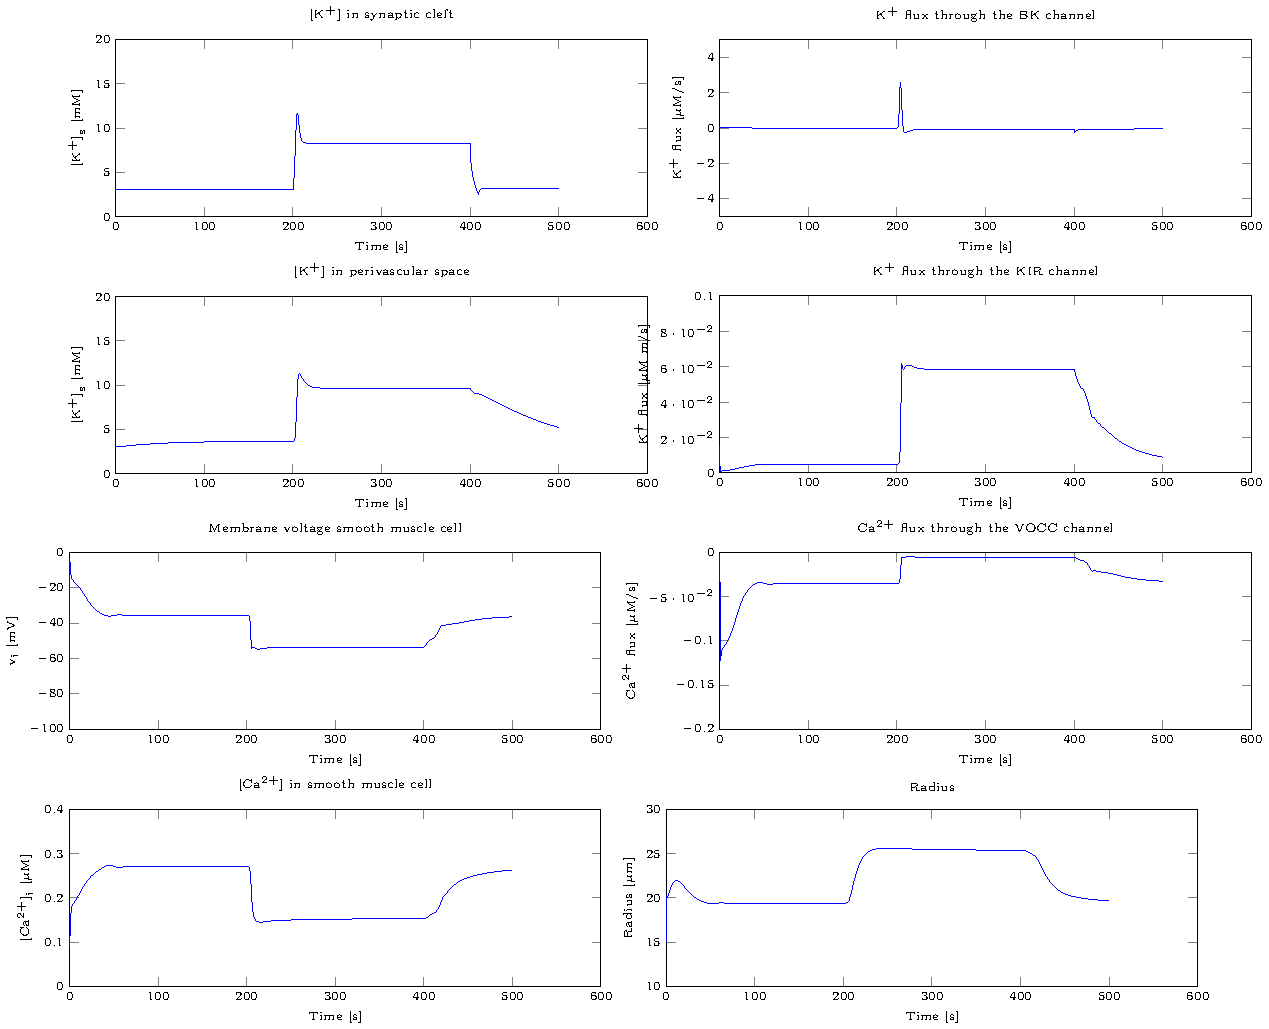
\includegraphics[height = \textwidth]{figures/6_Neuron_to_Radius.pdf}
			\caption{Summary describing effects from the input signal to radius change}
			\label{fig:6NtR}
		\end{figure}
		
	\end{landscape}
	
	
	\subsection{NVU1.1 compared to NVU1.0}
The main thing that stands out is the slow outflux of potassium in the perivascular space at the end of the pulse. (figure \ref{fig:NVU10a} bottom graph) This change is due to a smaller negative flux in the BK-channel, wich can be seen in figure \ref{fig:NVU10b} top right graph. This indicates that with the current calcium and EET  concentrations in the astrocyte, there are fewer open BK-channels compared to NVU1.0. Looking at the graphs in figure \ref{fig:NVU10b} this means that it takes a longer time to reach the steady state after the end of the pulse, resulting in smoother changes. Furthermore, the slower response has caused the over- and undershoots generated by NVU1.0 to disappear, which makes the results look more physiological. \cite{Hillman2011}

Figure \ref{fig:BKeff} shows the effects of different regulating mechanisms of the BK-channel. Blue line represents NVU 1.0 (depends only on membrane voltage), red is the result of NVU 1.1 (Depends on membrane voltage, \gls{Ca} concentration and EET concentration), green is NVU 1.1 without the effects of the calcium concentration, and black represents NVU 1.1 without the EET concentration playing a part. The black and green line don't represent physiological situations, but they provide insight in the effects of the separate systems. For the green line the Calcium concentration was simulated (otherwise there would have been no EET), but it was not used in the equations describing the opening of the BK-channel. ($v_3$ was replaced by the constant used in NVU1.0) The black line does the opposite, the EET voltage shift is ignored (as in NVU 1.0) and $v_3$ is changed to the \gls{Ca} dependent equation. It can be seen that adding the \gls{Ca} concentration to the equation describing the open state of the BK-channels leads to a decrease in negative flux through the BK-channel, and therefore leads to a slow restoration process. The EET concentration dependent voltage shift, contributing to the open state of the BK-channel has the opposite effect. It increases the negative \gls{K} flux torugh the BK-channel, creating similar results as NVU 1.0. The combination of these two effects (NVU 1.1) shows results that lay somewhere in between the previous results, generating a stable return to the steady state at a more realistic speed.
	
\begin{landscape}
	
	\begin{figure}[h!]
		\centering
		\tiny 
%%		\newlength\figureheight 
%%		\newlength\figurewidth 
		\setlength\figureheight{2 cm} 
		\setlength\figurewidth{18 cm}
		%% % This file was created by matlab2tikz v0.3.3.
% Copyright (c) 2008--2013, Nico Schlömer <nico.schloemer@gmail.com>
% All rights reserved.
% 
% The latest updates can be retrieved from
%   http://www.mathworks.com/matlabcentral/fileexchange/22022-matlab2tikz
% where you can also make suggestions and rate matlab2tikz.
% 
% 
% 
\begin{tikzpicture}

\begin{axis}[%
width=\figurewidth,
height=\figureheight,
scale only axis,
xmin=0,
xmax=500,
xlabel={Time [s]},
separate axis lines,
every outer y axis line/.append style={blue},
every y tick label/.append style={font=\color{blue}},
ymin=-5000,
ymax=5000,
ytick={-5000,     0,  5000},
ylabel={$\text{J}_{\text{BK}}\text{ [}\mu\text{M/s]}$},
name=plot3,
title={$\text{The contribution of the BK- and KIR-channel to K}_\text{p}\text{ for NVU}$}
]
\addplot [
color=blue,
solid,
forget plot
]
table[row sep=crcr]{
0 113.285245901639\\
0.00089136 112.878203971859\\
0.0017827 113.112280874371\\
0.0026741 113.282825798199\\
0.0061751 113.902463021875\\
0.0096762 114.481322357417\\
0.013177 115.027385130038\\
0.016678 115.537371683448\\
0.026472 116.801403669875\\
0.036266 117.857142857143\\
0.04606 118.739034188735\\
0.055854 119.471682025383\\
0.065648 120.078049420368\\
0.075699 120.582737587722\\
0.079199 120.735226601954\\
0.0827 120.876237948449\\
0.086201 121.00378756825\\
0.089702 121.121841643575\\
0.093202 121.228418239355\\
0.10095 121.431382193802\\
0.1087 121.590070666164\\
0.11645 121.707764952781\\
0.12421 121.79138247639\\
0.14151 121.856248155556\\
0.15881 121.785035084268\\
0.17612 121.605980621998\\
0.19342 121.336415351071\\
0.21073 120.994737791184\\
0.2497 120.026555635696\\
0.28868 118.878161522448\\
0.32765 117.626618587117\\
0.36662 116.319472899218\\
0.37628 115.991673905561\\
0.38594 115.660340249779\\
0.39561 115.32737851348\\
0.40527 114.994673440957\\
0.41493 114.660089156942\\
0.43002 114.137043774686\\
0.44221 113.712347176243\\
0.4544 113.289521124914\\
0.46659 112.86484537603\\
0.47879 112.440183546378\\
0.49098 112.017371353655\\
0.51139 111.305758578873\\
0.52695 110.766608764052\\
0.54251 110.227291349163\\
0.55807 109.689630309386\\
0.57363 109.153625563294\\
0.58919 108.619277029463\\
0.6088 107.948940632835\\
0.6284 107.283661330231\\
0.64801 106.618273579341\\
0.66761 105.957823329892\\
0.68722 105.300671800754\\
0.73766 103.629243675449\\
0.78811 101.982501556509\\
0.83855 100.362081394587\\
0.889 98.7679806022478\\
0.93944 97.2017890201347\\
1.0031 95.2638390589931\\
1.0667 93.3669708238455\\
1.1303 91.5111802768449\\
1.1939 89.6964633806739\\
1.2576 87.9226182675927\\
1.3769 84.6996773189628\\
1.4783 82.0647634022898\\
1.5797 79.5217426910163\\
1.6811 77.0669549266247\\
1.7825 74.6961905073864\\
1.8839 72.4070161646931\\
2.0684 68.4402738200518\\
2.2528 64.71243285733\\
2.4373 61.205908361445\\
2.6218 57.9068891545352\\
2.8063 54.7970328644648\\
2.9907 51.8683477976093\\
3.3424 46.736638721509\\
3.694 42.1380970314214\\
4.0456 38.0079903068409\\
4.3972 34.290626279165\\
4.7489 30.9417774575938\\
5.2238 26.9336564280568\\
5.6986 23.4376279123074\\
6.1735 20.384105309691\\
6.6484 17.7104310951749\\
7.1233 15.3688725891483\\
7.8241 12.4291889059891\\
8.525 10.0004911752186\\
9.2258 7.98896493008939\\
9.9266 6.31962408723272\\
10.627 4.93139919447264\\
11.627 3.34359343789908\\
12.627 2.11319951537378\\
13.627 1.15228069026491\\
14.627 0.395674383575101\\
15.627 -0.206260846786077\\
16.627 -0.691394610170601\\
17.627 -1.08886996954714\\
18.627 -1.42226333540718\\
19.627 -1.70699760961394\\
20.627 -1.95471364484757\\
21.627 -2.17459641769541\\
22.627 -2.37254003078031\\
23.627 -2.55361996136088\\
24.627 -2.72160188611284\\
25.627 -2.87910540620191\\
26.627 -3.02711287206523\\
27.627 -3.16677035921281\\
28.627 -3.29889649300894\\
29.627 -3.42414617374505\\
30.627 -3.54268312649399\\
31.627 -3.6551622515472\\
32.627 -3.76158354890468\\
33.627 -3.86227446871214\\
34.627 -3.95788991126101\\
35.627 -4.0484298765513\\
36.627 -4.13422181472871\\
37.627 -4.21559317593896\\
38.627 -4.29270768525492\\
39.627 -4.36556534267658\\
40.627 -4.43432987327679\\
41.627 -4.49818265169128\\
42.627 -4.55663250270146\\
43.627 -4.6086970758702\\
44.627 -4.65323029568748\\
45.627 -4.68908608664331\\
46.627 -4.71528209830053\\
47.627 -4.7316546055863\\
48.627 -4.73836733357346\\
49.627 -4.73689380791774\\
50.627 -4.72870755427486\\
51.627 -4.71610072366482\\
52.627 -4.70103801696192\\
53.627 -4.68532040996758\\
54.627 -4.67058515341039\\
55.627 -4.65765087265464\\
56.627 -4.64717246799175\\
57.627 -4.63931366449458\\
58.627 -4.63407446216314\\
59.627 -4.63129113592455\\
60.627 -4.63063623563312\\
61.627 -4.63178231114313\\
62.627 -4.63440191230885\\
63.627 -4.63816758898458\\
64.627 -4.64275189102459\\
65.627 -4.64782736828318\\
66.627 -4.65306657061462\\
67.627 -4.65830577294607\\
68.627 -4.66338125020466\\
69.627 -4.66780182717181\\
70.627 -4.67189495399325\\
71.627 -4.67516945545041\\
72.627 -4.67778905661613\\
73.627 -4.67959003241756\\
74.627 -4.68073610792757\\
75.627 -4.681391008219\\
76.627 -4.68122728314614\\
77.627 -4.68089983300043\\
78.627 -4.68008120763614\\
79.627 -4.67893513212613\\
80.627 -4.67778905661613\\
81.627 -4.67664298110613\\
82.627 -4.67533318052327\\
83.627 -4.67435083008612\\
84.627 -4.67336847964897\\
85.627 -4.67254985428468\\
86.627 -4.67205867906611\\
87.627 -4.6717312289204\\
88.627 -4.67156750384754\\
89.627 -4.67140377877468\\
90.627 -4.67156750384754\\
91.627 -4.67189495399325\\
92.627 -4.67222240413897\\
93.627 -4.67254985428468\\
94.627 -4.67304102950326\\
95.627 -4.67336847964897\\
96.627 -4.67369592979469\\
97.627 -4.67418710501326\\
98.627 -4.67435083008612\\
99.627 -4.67467828023183\\
100.63 -4.67484200530469\\
101.63 -4.67500573037755\\
102.63 -4.67516945545041\\
103.63 -4.67516945545041\\
104.63 -4.67516945545041\\
105.63 -4.67516945545041\\
106.63 -4.67516945545041\\
107.63 -4.67500573037755\\
108.63 -4.67500573037755\\
109.63 -4.67500573037755\\
110.63 -4.67484200530469\\
111.63 -4.67484200530469\\
112.63 -4.67467828023183\\
113.63 -4.67467828023183\\
114.63 -4.67467828023183\\
115.63 -4.67451455515898\\
116.63 -4.67451455515898\\
117.63 -4.67451455515898\\
118.63 -4.67451455515898\\
119.63 -4.67451455515898\\
120.63 -4.67451455515898\\
121.63 -4.67451455515898\\
122.63 -4.67451455515898\\
123.63 -4.67451455515898\\
124.63 -4.67467828023183\\
125.63 -4.67467828023183\\
126.63 -4.67467828023183\\
127.63 -4.67467828023183\\
128.63 -4.67467828023183\\
129.63 -4.67467828023183\\
130.63 -4.67467828023183\\
131.63 -4.67467828023183\\
132.63 -4.67467828023183\\
133.63 -4.67467828023183\\
134.63 -4.67467828023183\\
135.63 -4.67467828023183\\
136.63 -4.67467828023183\\
137.63 -4.67467828023183\\
138.63 -4.67467828023183\\
139.63 -4.67467828023183\\
140.63 -4.67467828023183\\
141.63 -4.67467828023183\\
142.63 -4.67467828023183\\
143.63 -4.67467828023183\\
144.63 -4.67467828023183\\
145.63 -4.67467828023183\\
146.63 -4.67467828023183\\
147.63 -4.67467828023183\\
148.63 -4.67467828023183\\
149.63 -4.67467828023183\\
150.63 -4.67467828023183\\
151.63 -4.67467828023183\\
152.63 -4.67467828023183\\
153.63 -4.67467828023183\\
154.63 -4.67467828023183\\
155.63 -4.67467828023183\\
156.63 -4.67467828023183\\
157.63 -4.67467828023183\\
158.63 -4.67467828023183\\
159.63 -4.67467828023183\\
160.63 -4.67467828023183\\
161.63 -4.67467828023183\\
162.63 -4.67467828023183\\
163.63 -4.67467828023183\\
164.63 -4.67467828023183\\
165.63 -4.67467828023183\\
166.63 -4.67467828023183\\
167.63 -4.67467828023183\\
168.63 -4.67467828023183\\
169.63 -4.67467828023183\\
170.63 -4.67467828023183\\
171.63 -4.67467828023183\\
172.63 -4.67467828023183\\
173.63 -4.67467828023183\\
174.63 -4.67467828023183\\
175.63 -4.67467828023183\\
176.63 -4.67467828023183\\
177.63 -4.67467828023183\\
178.63 -4.67467828023183\\
179.63 -4.67467828023183\\
180.63 -4.67467828023183\\
181.63 -4.67467828023183\\
182.63 -4.67467828023183\\
183.63 -4.67467828023183\\
184.63 -4.67467828023183\\
185.63 -4.67467828023183\\
186.63 -4.67467828023183\\
187.63 -4.67467828023183\\
188.63 -4.67467828023183\\
189.63 -4.67467828023183\\
190.63 -4.67467828023183\\
191.63 -4.67467828023183\\
192.63 -4.67467828023183\\
193.63 -4.67467828023183\\
194.63 -4.67467828023183\\
195.63 -4.67467828023183\\
196.63 -4.67467828023183\\
197.19 -4.67467828023183\\
197.62 -4.67467828023183\\
197.92 -4.67467828023183\\
198.17 -4.67467828023183\\
198.37 -4.67467828023183\\
198.57 -4.67467828023183\\
198.71 -4.67467828023183\\
198.85 -4.67467828023183\\
198.97 -4.67467828023183\\
199.09 -4.67467828023183\\
199.21 -4.67467828023183\\
199.4 -4.67467828023183\\
199.6 -4.67467828023183\\
199.8 -4.67467828023183\\
199.99 -4.67467828023183\\
200.31 40.4227191121266\\
200.54 132.578861788618\\
200.77 287.879033171979\\
201.01 510.997244646396\\
201.24 804.941399047634\\
201.54 1289.85968879899\\
201.84 1889.51097614981\\
202.14 2549.14892280636\\
202.43 3151.79100289927\\
202.73 3573.00902071825\\
203.03 3730.64635045466\\
203.33 3595.64441597658\\
203.42 3500.4337305392\\
203.51 3382.13407040671\\
203.6 3244.36967657846\\
203.69 3090.77984149071\\
203.78 2924.16374833957\\
203.89 2697.58337724912\\
204 2459.22076361561\\
204.12 2213.43162815787\\
204.23 1963.67441512819\\
204.34 1713.84679632502\\
204.53 1319.70514363844\\
204.71 942.64978153003\\
204.89 590.486314111082\\
205.08 268.674290928894\\
205.45 -285.093367675467\\
205.83 -682.111394248271\\
206.2 -925.025373350732\\
206.58 -1036.13221994279\\
207.23 -1009.83479273606\\
207.87 -851.895378000717\\
208.52 -666.628530568466\\
209.17 -501.485247493645\\
209.82 -374.605847018705\\
210.52 -272.003992300563\\
211.23 -195.921101388137\\
211.93 -144.870132645647\\
212.64 -114.620874346519\\
213.34 -96.010539809144\\
214.34 -79.1862485402603\\
215.34 -68.588191734784\\
216.34 -62.6030615877537\\
217.34 -59.6146726283713\\
218.34 -58.0332350805246\\
219.34 -57.0521309467868\\
220.34 -56.5230392436065\\
221.34 -56.1955345446261\\
222.34 -56.0146949934499\\
223.34 -55.9150196502819\\
224.34 -55.856638377855\\
225.34 -55.8224639744831\\
226.34 -55.806800706271\\
227.34 -55.7996810389019\\
228.34 -55.7954092384804\\
229.34 -55.7911374380589\\
230.34 -55.7854417041636\\
231.34 -55.7825938372159\\
232.34 -55.7811699037421\\
233.34 -55.7783220367944\\
234.34 -55.7754741698468\\
235.34 -55.7712023694253\\
236.34 -55.7683545024776\\
237.34 -55.76550663553\\
238.34 -55.7640827020562\\
239.34 -55.7612348351085\\
240.34 -55.7598109016347\\
241.34 -55.756963034687\\
242.34 -55.7541151677394\\
243.34 -55.7526912342655\\
244.34 -55.7512673007917\\
245.34 -55.7498433673179\\
246.34 -55.7484194338441\\
247.34 -55.7469955003702\\
248.34 -55.7455715668964\\
249.34 -55.7441476334226\\
250.34 -55.7427236999487\\
251.34 -55.7412997664749\\
252.34 -55.7398758330011\\
253.34 -55.7398758330011\\
254.34 -55.7384518995273\\
255.34 -55.7370279660534\\
256.34 -55.7356040325796\\
257.34 -55.7341800991058\\
258.34 -55.7341800991058\\
259.34 -55.7327561656319\\
260.34 -55.7313322321581\\
261.34 -55.7299082986843\\
262.34 -55.7284843652105\\
263.34 -55.7284843652105\\
264.34 -55.7270604317366\\
265.34 -55.7256364982628\\
266.34 -55.724212564789\\
267.34 -55.724212564789\\
268.34 -55.7227886313151\\
269.34 -55.7213646978413\\
270.34 -55.7213646978413\\
271.34 -55.7199407643675\\
272.34 -55.7185168308937\\
273.34 -55.7185168308937\\
274.34 -55.7170928974198\\
275.34 -55.7170928974198\\
276.34 -55.715668963946\\
277.34 -55.715668963946\\
278.34 -55.7142450304722\\
279.34 -55.7142450304722\\
280.34 -55.7128210969984\\
281.34 -55.7128210969984\\
282.34 -55.7113971635245\\
283.34 -55.7113971635245\\
284.34 -55.7099732300507\\
285.34 -55.7099732300507\\
286.34 -55.7085492965769\\
287.34 -55.7085492965769\\
288.34 -55.7085492965769\\
289.34 -55.707125363103\\
290.34 -55.707125363103\\
291.34 -55.7057014296292\\
292.34 -55.7057014296292\\
293.34 -55.7057014296292\\
294.34 -55.7042774961554\\
295.34 -55.7042774961554\\
296.34 -55.7042774961554\\
297.34 -55.7028535626816\\
298.34 -55.7028535626816\\
299.34 -55.7028535626816\\
300.34 -55.7014296292077\\
301.34 -55.7014296292077\\
302.34 -55.7014296292077\\
303.34 -55.7014296292077\\
304.34 -55.7000056957339\\
305.34 -55.7000056957339\\
306.34 -55.7000056957339\\
307.34 -55.7000056957339\\
308.34 -55.6985817622601\\
309.34 -55.6985817622601\\
310.34 -55.6985817622601\\
311.34 -55.6985817622601\\
312.34 -55.6971578287862\\
313.34 -55.6971578287862\\
314.34 -55.6971578287862\\
315.34 -55.6971578287862\\
316.34 -55.6957338953124\\
317.34 -55.6957338953124\\
318.34 -55.6957338953124\\
319.34 -55.6957338953124\\
320.34 -55.6957338953124\\
321.34 -55.6957338953124\\
322.34 -55.6943099618386\\
323.34 -55.6943099618386\\
324.34 -55.6943099618386\\
325.34 -55.6943099618386\\
326.34 -55.6943099618386\\
327.34 -55.6943099618386\\
328.34 -55.6928860283648\\
329.34 -55.6928860283648\\
330.34 -55.6928860283648\\
331.34 -55.6928860283648\\
332.34 -55.6928860283648\\
333.34 -55.6928860283648\\
334.34 -55.6928860283648\\
335.34 -55.6914620948909\\
336.34 -55.6914620948909\\
337.34 -55.6914620948909\\
338.34 -55.6914620948909\\
339.34 -55.6914620948909\\
340.34 -55.6914620948909\\
341.34 -55.6914620948909\\
342.34 -55.6914620948909\\
343.34 -55.6914620948909\\
344.34 -55.6900381614171\\
345.34 -55.6900381614171\\
346.34 -55.6900381614171\\
347.34 -55.6900381614171\\
348.34 -55.6900381614171\\
349.34 -55.6900381614171\\
350.34 -55.6900381614171\\
351.34 -55.6900381614171\\
352.34 -55.6900381614171\\
353.34 -55.6900381614171\\
354.34 -55.6900381614171\\
355.34 -55.6886142279433\\
356.34 -55.6886142279433\\
357.34 -55.6886142279433\\
358.34 -55.6886142279433\\
359.34 -55.6886142279433\\
360.34 -55.6886142279433\\
361.34 -55.6886142279433\\
362.34 -55.6886142279433\\
363.34 -55.6886142279433\\
364.34 -55.6886142279433\\
365.34 -55.6886142279433\\
366.34 -55.6886142279433\\
367.34 -55.6886142279433\\
368.34 -55.6886142279433\\
369.34 -55.6886142279433\\
370.34 -55.6886142279433\\
371.34 -55.6871902944694\\
372.34 -55.6871902944694\\
373.34 -55.6871902944694\\
374.34 -55.6871902944694\\
375.34 -55.6871902944694\\
376.34 -55.6871902944694\\
377.34 -55.6871902944694\\
378.34 -55.6871902944694\\
379.34 -55.6871902944694\\
380.34 -55.6871902944694\\
381.34 -55.6871902944694\\
382.34 -55.6871902944694\\
383.34 -55.6871902944694\\
384.34 -55.6871902944694\\
385.34 -55.6871902944694\\
386.34 -55.6871902944694\\
387.34 -55.6871902944694\\
388.34 -55.6871902944694\\
389.34 -55.6871902944694\\
390.34 -55.6871902944694\\
391.34 -55.6871902944694\\
392.34 -55.6871902944694\\
393.34 -55.6871902944694\\
394.34 -55.6871902944694\\
395.34 -55.6871902944694\\
396.34 -55.6871902944694\\
397.34 -55.6871902944694\\
398.17 -55.6871902944694\\
398.58 -55.6871902944694\\
398.9 -55.6857663609956\\
399.16 -55.6857663609956\\
399.42 -55.6857663609956\\
399.62 -55.6857663609956\\
399.82 -55.6857663609956\\
399.88 -55.6857663609956\\
399.94 -55.6857663609956\\
399.99 -55.6857663609956\\
400.03 -613.773265169531\\
400.08 -1068.24946947147\\
400.15 -1510.61404758513\\
400.22 -1657.63968072976\\
400.29 -1645.34759358289\\
400.36 -1575.16265266522\\
400.48 -1451.3595338741\\
400.59 -1345.36436147403\\
400.71 -1263.00652472527\\
400.83 -1196.37332416638\\
401.11 -1062.78722426471\\
401.23 -1014.53734991732\\
401.33 -977.660386049257\\
401.41 -948.929610741349\\
401.5 -921.34556045794\\
401.56 -899.920640646418\\
401.63 -879.272254710851\\
401.66 -868.478072456232\\
401.69 -860.026587290119\\
401.72 -851.673050516731\\
401.75 -843.485678758874\\
401.78 -835.423265500933\\
401.81 -824.950804491261\\
401.85 -814.715631921023\\
401.89 -804.715218745022\\
401.93 -794.926402410756\\
401.98 -781.348757646922\\
402.03 -768.200873235759\\
402.09 -755.457501161171\\
402.14 -743.104875604549\\
402.2 -731.129196337742\\
402.37 -693.788684191364\\
402.55 -660.001751364605\\
402.68 -637.826697070689\\
402.81 -617.085132859966\\
402.93 -597.627496407519\\
403.06 -579.336172712586\\
403.27 -551.105155428588\\
403.44 -530.892617350628\\
403.6 -512.081509523246\\
403.77 -494.494746669433\\
403.93 -478.021325254685\\
404.15 -457.72833549271\\
404.37 -439.014919577652\\
404.59 -421.671409315561\\
404.81 -405.56615250597\\
405.2 -379.667924528302\\
405.58 -356.512241740238\\
405.97 -335.619988414281\\
406.36 -316.594923329095\\
406.74 -299.145693835142\\
407.4 -272.36756354157\\
408.07 -248.811534371677\\
408.61 -231.012508850602\\
409.16 -214.719848053181\\
409.32 -210.204211060375\\
409.48 -205.796871277694\\
409.65 -201.479478205536\\
409.81 -197.28476504613\\
409.97 -193.216822280744\\
410.14 -178.135644720219\\
410.3 -186.894020737512\\
410.47 -207.784075400202\\
410.63 -202.390143472946\\
410.8 -180.192372758471\\
410.96 -174.310150072616\\
411.13 -176.984858033968\\
411.38 -171.686259270054\\
411.64 -153.124087591241\\
411.89 -141.657325730624\\
412.14 -136.666178695164\\
412.4 -128.909659349964\\
412.65 -119.126707305147\\
413.05 -106.349335857185\\
413.31 -100.801724278693\\
413.53 -95.0912328274826\\
413.72 -89.9944440813125\\
413.89 -86.0477280156914\\
414.02 -83.1973712174467\\
414.15 -80.4182540590919\\
414.28 -77.7183600713012\\
414.41 -75.1099916586251\\
414.63 -71.0448396014985\\
414.85 -67.222958490813\\
415.07 -63.6278841433481\\
415.47 -57.4211077648291\\
415.87 -51.843302884458\\
416.28 -46.856478601133\\
416.68 -42.4024102698454\\
417.45 -35.1608941292066\\
418.22 -29.2985702821768\\
418.99 -24.5389629532576\\
419.75 -20.6708485513537\\
420.75 -16.6814072327044\\
421.75 -13.6381354821803\\
422.75 -11.3253406708595\\
423.75 -9.57448899371069\\
424.75 -8.25520833333333\\
425.75 -7.2667714884696\\
426.75 -6.5310534591195\\
427.75 -5.99269523060797\\
428.75 -5.6028891509434\\
429.75 -5.32199947589099\\
430.75 -5.12169156184486\\
431.75 -4.98116483228512\\
432.75 -4.88485980083857\\
433.75 -4.82016509433962\\
434.75 -4.77807258909853\\
435.75 -4.75088443396226\\
436.75 -4.73319575471698\\
437.75 -4.72140330188679\\
438.75 -4.71239517819707\\
439.75 -4.70469732704403\\
440.75 -4.69732704402516\\
441.75 -4.68995676100629\\
442.75 -4.68258647798742\\
443.75 -4.67505241090147\\
444.75 -4.6676821278826\\
445.75 -4.6606394129979\\
446.75 -4.65441561844864\\
447.75 -4.64868317610063\\
448.75 -4.64393343815514\\
449.75 -4.64000262054507\\
450.75 -4.63689072327044\\
451.75 -4.63459774633124\\
452.75 -4.63312368972746\\
453.75 -4.63214098532495\\
454.75 -4.63164963312369\\
455.75 -4.63164963312369\\
456.75 -4.63197720125786\\
457.75 -4.63263233752621\\
458.75 -4.63328747379455\\
459.75 -4.63410639412998\\
460.75 -4.63508909853249\\
461.75 -4.63590801886792\\
462.75 -4.63656315513627\\
463.75 -4.63721829140461\\
464.75 -4.63787342767296\\
465.75 -4.63820099580713\\
466.75 -4.6385285639413\\
467.75 -4.63869234800839\\
468.75 -4.63885613207547\\
469.75 -4.63885613207547\\
470.75 -4.63869234800839\\
471.75 -4.6385285639413\\
472.75 -4.63836477987421\\
473.75 -4.63820099580713\\
474.75 -4.63787342767296\\
475.75 -4.63770964360587\\
476.75 -4.63754585953878\\
477.75 -4.6373820754717\\
478.75 -4.63721829140461\\
479.75 -4.63705450733753\\
480.75 -4.63705450733753\\
481.75 -4.63689072327044\\
482.75 -4.63689072327044\\
483.75 -4.63689072327044\\
484.75 -4.63689072327044\\
485.75 -4.63689072327044\\
486.75 -4.63689072327044\\
487.75 -4.63705450733753\\
488.75 -4.63705450733753\\
489.75 -4.63705450733753\\
490.75 -4.63721829140461\\
491.75 -4.63721829140461\\
492.75 -4.63721829140461\\
493.75 -4.63721829140461\\
494.75 -4.63721829140461\\
495.75 -4.6373820754717\\
496.75 -4.6373820754717\\
497.75 -4.6373820754717\\
498.75 -4.6373820754717\\
499.75 -4.6373820754717\\
500 -4.6373820754717\\
};
\end{axis}

\begin{axis}[%
width=\figurewidth,
height=\figureheight,
scale only axis,
xmin=0,
xmax=500,
every outer y axis line/.append style={green!50!black},
every y tick label/.append style={font=\color{green!50!black}},
ymin=0,
ymax=100,
ytick={  0,  50, 100},
ylabel={$\text{J}_{\text{KIR}}\text{ [}\mu\text{M/s]}$},
axis x line*=bottom,
axis y line*=right
]
\addplot [
color=green!50!black,
solid,
forget plot
]
table[row sep=crcr]{
0 14.771\\
0.00089136 14.722\\
0.0017827 14.673\\
0.0026741 14.622\\
0.0061751 14.419\\
0.0096762 14.207\\
0.013177 13.99\\
0.016678 13.768\\
0.026472 13.137\\
0.036266 12.509\\
0.04606 11.901\\
0.055854 11.32\\
0.065648 10.769\\
0.075699 10.236\\
0.079199 10.058\\
0.0827 9.8839\\
0.086201 9.7134\\
0.089702 9.5465\\
0.093202 9.3833\\
0.10095 9.0341\\
0.1087 8.701\\
0.11645 8.383\\
0.12421 8.079\\
0.14151 7.4452\\
0.15881 6.8649\\
0.17612 6.3282\\
0.19342 5.8262\\
0.21073 5.3513\\
0.2497 4.3442\\
0.28868 3.3755\\
0.32765 2.4184\\
0.36662 1.5557\\
0.37628 1.3715\\
0.38594 1.2078\\
0.39561 1.067\\
0.40527 0.94932\\
0.41493 0.8537\\
0.43002 0.74278\\
0.44221 0.68184\\
0.4544 0.64068\\
0.46659 0.61457\\
0.47879 0.59956\\
0.49098 0.59256\\
0.51139 0.59263\\
0.52695 0.59831\\
0.54251 0.60638\\
0.55807 0.61553\\
0.57363 0.62504\\
0.58919 0.63452\\
0.6088 0.64615\\
0.6284 0.65732\\
0.64801 0.66808\\
0.66761 0.67854\\
0.68722 0.68878\\
0.73766 0.71442\\
0.78811 0.73938\\
0.83855 0.7637\\
0.889 0.78733\\
0.93944 0.81024\\
1.0031 0.83817\\
1.0667 0.86506\\
1.1303 0.89087\\
1.1939 0.91561\\
1.2576 0.93926\\
1.3769 0.9808\\
1.4783 1.0133\\
1.5797 1.0434\\
1.6811 1.0711\\
1.7825 1.0966\\
1.8839 1.1201\\
2.0684 1.158\\
2.2528 1.1906\\
2.4373 1.2185\\
2.6218 1.2428\\
2.8063 1.2641\\
2.9907 1.2833\\
3.3424 1.3144\\
3.694 1.3411\\
4.0456 1.3654\\
4.3972 1.3884\\
4.7489 1.4104\\
5.2238 1.4393\\
5.6986 1.4678\\
6.1735 1.4963\\
6.6484 1.525\\
7.1233 1.5538\\
7.8241 1.597\\
8.525 1.6414\\
9.2258 1.6872\\
9.9266 1.7348\\
10.627 1.7844\\
11.627 1.8594\\
12.627 1.9399\\
13.627 2.0268\\
14.627 2.1206\\
15.627 2.2217\\
16.627 2.33\\
17.627 2.4451\\
18.627 2.5663\\
19.627 2.6925\\
20.627 2.8216\\
21.627 2.9516\\
22.627 3.0801\\
23.627 3.2071\\
24.627 3.332\\
25.627 3.4522\\
26.627 3.5665\\
27.627 3.6762\\
28.627 3.7814\\
29.627 3.8815\\
30.627 3.9763\\
31.627 4.0659\\
32.627 4.1506\\
33.627 4.231\\
34.627 4.3072\\
35.627 4.3795\\
36.627 4.4481\\
37.627 4.5133\\
38.627 4.5749\\
39.627 4.6322\\
40.627 4.6839\\
41.627 4.7289\\
42.627 4.7653\\
43.627 4.7911\\
44.627 4.8049\\
45.627 4.8059\\
46.627 4.7951\\
47.627 4.7744\\
48.627 4.7471\\
49.627 4.7172\\
50.627 4.6882\\
51.627 4.6627\\
52.627 4.6424\\
53.627 4.6277\\
54.627 4.6184\\
55.627 4.6137\\
56.627 4.6128\\
57.627 4.6148\\
58.627 4.6191\\
59.627 4.6249\\
60.627 4.6317\\
61.627 4.6391\\
62.627 4.6466\\
63.627 4.6541\\
64.627 4.6611\\
65.627 4.6675\\
66.627 4.6731\\
67.627 4.6777\\
68.627 4.6814\\
69.627 4.684\\
70.627 4.6856\\
71.627 4.6862\\
72.627 4.6861\\
73.627 4.6852\\
74.627 4.6839\\
75.627 4.6822\\
76.627 4.6803\\
77.627 4.6783\\
78.627 4.6765\\
79.627 4.6747\\
80.627 4.6732\\
81.627 4.672\\
82.627 4.6711\\
83.627 4.6705\\
84.627 4.6702\\
85.627 4.6701\\
86.627 4.6703\\
87.627 4.6707\\
88.627 4.6711\\
89.627 4.6717\\
90.627 4.6723\\
91.627 4.6729\\
92.627 4.6735\\
93.627 4.6741\\
94.627 4.6745\\
95.627 4.6749\\
96.627 4.6752\\
97.627 4.6754\\
98.627 4.6755\\
99.627 4.6756\\
100.63 4.6756\\
101.63 4.6755\\
102.63 4.6755\\
103.63 4.6754\\
104.63 4.6752\\
105.63 4.6751\\
106.63 4.675\\
107.63 4.6748\\
108.63 4.6747\\
109.63 4.6746\\
110.63 4.6746\\
111.63 4.6745\\
112.63 4.6745\\
113.63 4.6745\\
114.63 4.6745\\
115.63 4.6745\\
116.63 4.6745\\
117.63 4.6745\\
118.63 4.6745\\
119.63 4.6746\\
120.63 4.6746\\
121.63 4.6746\\
122.63 4.6746\\
123.63 4.6747\\
124.63 4.6747\\
125.63 4.6747\\
126.63 4.6747\\
127.63 4.6747\\
128.63 4.6747\\
129.63 4.6748\\
130.63 4.6748\\
131.63 4.6747\\
132.63 4.6747\\
133.63 4.6747\\
134.63 4.6747\\
135.63 4.6747\\
136.63 4.6747\\
137.63 4.6747\\
138.63 4.6747\\
139.63 4.6747\\
140.63 4.6747\\
141.63 4.6747\\
142.63 4.6747\\
143.63 4.6747\\
144.63 4.6747\\
145.63 4.6747\\
146.63 4.6747\\
147.63 4.6747\\
148.63 4.6747\\
149.63 4.6747\\
150.63 4.6747\\
151.63 4.6747\\
152.63 4.6747\\
153.63 4.6747\\
154.63 4.6747\\
155.63 4.6747\\
156.63 4.6747\\
157.63 4.6747\\
158.63 4.6747\\
159.63 4.6747\\
160.63 4.6747\\
161.63 4.6747\\
162.63 4.6747\\
163.63 4.6747\\
164.63 4.6747\\
165.63 4.6747\\
166.63 4.6747\\
167.63 4.6747\\
168.63 4.6747\\
169.63 4.6747\\
170.63 4.6747\\
171.63 4.6747\\
172.63 4.6747\\
173.63 4.6747\\
174.63 4.6747\\
175.63 4.6747\\
176.63 4.6747\\
177.63 4.6747\\
178.63 4.6747\\
179.63 4.6747\\
180.63 4.6747\\
181.63 4.6747\\
182.63 4.6747\\
183.63 4.6747\\
184.63 4.6747\\
185.63 4.6747\\
186.63 4.6747\\
187.63 4.6747\\
188.63 4.6747\\
189.63 4.6747\\
190.63 4.6747\\
191.63 4.6747\\
192.63 4.6747\\
193.63 4.6747\\
194.63 4.6747\\
195.63 4.6747\\
196.63 4.6747\\
197.19 4.6747\\
197.62 4.6747\\
197.92 4.6747\\
198.17 4.6747\\
198.37 4.6747\\
198.57 4.6747\\
198.71 4.6747\\
198.85 4.6747\\
198.97 4.6747\\
199.09 4.6747\\
199.21 4.6747\\
199.4 4.6747\\
199.6 4.6747\\
199.8 4.6747\\
199.99 4.6747\\
200.31 4.6892\\
200.54 4.728\\
200.77 4.8197\\
201.01 4.9958\\
201.24 5.2965\\
201.54 5.9552\\
201.84 7.1169\\
202.14 9.1565\\
202.43 12.756\\
202.73 19.137\\
203.03 30.407\\
203.33 48.232\\
203.42 54.082\\
203.51 58.949\\
203.6 61.92\\
203.69 62.673\\
203.78 61.808\\
203.89 59.759\\
204 57.689\\
204.12 55.78\\
204.23 53.959\\
204.34 52.34\\
204.53 50.389\\
204.71 49.148\\
204.89 48.407\\
205.08 48.146\\
205.45 48.745\\
205.83 50.389\\
206.2 52.54\\
206.58 54.801\\
207.23 58.179\\
207.87 60.254\\
208.52 60.967\\
209.17 60.746\\
209.82 60.069\\
210.52 59.191\\
211.23 58.34\\
211.93 57.632\\
212.64 57.102\\
213.34 56.715\\
214.34 56.341\\
215.34 56.104\\
216.34 55.967\\
217.34 55.895\\
218.34 55.854\\
219.34 55.83\\
220.34 55.816\\
221.34 55.808\\
222.34 55.803\\
223.34 55.799\\
224.34 55.797\\
225.34 55.794\\
226.34 55.793\\
227.34 55.791\\
228.34 55.789\\
229.34 55.787\\
230.34 55.784\\
231.34 55.781\\
232.34 55.779\\
233.34 55.776\\
234.34 55.773\\
235.34 55.77\\
236.34 55.767\\
237.34 55.765\\
238.34 55.763\\
239.34 55.76\\
240.34 55.758\\
241.34 55.756\\
242.34 55.754\\
243.34 55.752\\
244.34 55.75\\
245.34 55.749\\
246.34 55.747\\
247.34 55.746\\
248.34 55.745\\
249.34 55.744\\
250.34 55.742\\
251.34 55.741\\
252.34 55.74\\
253.34 55.739\\
254.34 55.738\\
255.34 55.737\\
256.34 55.735\\
257.34 55.734\\
258.34 55.733\\
259.34 55.732\\
260.34 55.731\\
261.34 55.73\\
262.34 55.729\\
263.34 55.728\\
264.34 55.727\\
265.34 55.725\\
266.34 55.724\\
267.34 55.723\\
268.34 55.722\\
269.34 55.722\\
270.34 55.721\\
271.34 55.72\\
272.34 55.719\\
273.34 55.718\\
274.34 55.717\\
275.34 55.716\\
276.34 55.716\\
277.34 55.715\\
278.34 55.714\\
279.34 55.713\\
280.34 55.713\\
281.34 55.712\\
282.34 55.711\\
283.34 55.711\\
284.34 55.71\\
285.34 55.71\\
286.34 55.709\\
287.34 55.708\\
288.34 55.708\\
289.34 55.707\\
290.34 55.707\\
291.34 55.706\\
292.34 55.706\\
293.34 55.705\\
294.34 55.705\\
295.34 55.704\\
296.34 55.704\\
297.34 55.703\\
298.34 55.703\\
299.34 55.702\\
300.34 55.702\\
301.34 55.702\\
302.34 55.701\\
303.34 55.701\\
304.34 55.7\\
305.34 55.7\\
306.34 55.7\\
307.34 55.699\\
308.34 55.699\\
309.34 55.699\\
310.34 55.698\\
311.34 55.698\\
312.34 55.698\\
313.34 55.697\\
314.34 55.697\\
315.34 55.697\\
316.34 55.696\\
317.34 55.696\\
318.34 55.696\\
319.34 55.696\\
320.34 55.695\\
321.34 55.695\\
322.34 55.695\\
323.34 55.695\\
324.34 55.694\\
325.34 55.694\\
326.34 55.694\\
327.34 55.694\\
328.34 55.694\\
329.34 55.693\\
330.34 55.693\\
331.34 55.693\\
332.34 55.693\\
333.34 55.693\\
334.34 55.692\\
335.34 55.692\\
336.34 55.692\\
337.34 55.692\\
338.34 55.692\\
339.34 55.692\\
340.34 55.691\\
341.34 55.691\\
342.34 55.691\\
343.34 55.691\\
344.34 55.691\\
345.34 55.691\\
346.34 55.69\\
347.34 55.69\\
348.34 55.69\\
349.34 55.69\\
350.34 55.69\\
351.34 55.69\\
352.34 55.69\\
353.34 55.69\\
354.34 55.69\\
355.34 55.689\\
356.34 55.689\\
357.34 55.689\\
358.34 55.689\\
359.34 55.689\\
360.34 55.689\\
361.34 55.689\\
362.34 55.689\\
363.34 55.689\\
364.34 55.689\\
365.34 55.688\\
366.34 55.688\\
367.34 55.688\\
368.34 55.688\\
369.34 55.688\\
370.34 55.688\\
371.34 55.688\\
372.34 55.688\\
373.34 55.688\\
374.34 55.688\\
375.34 55.688\\
376.34 55.688\\
377.34 55.688\\
378.34 55.688\\
379.34 55.688\\
380.34 55.687\\
381.34 55.687\\
382.34 55.687\\
383.34 55.687\\
384.34 55.687\\
385.34 55.687\\
386.34 55.687\\
387.34 55.687\\
388.34 55.687\\
389.34 55.687\\
390.34 55.687\\
391.34 55.687\\
392.34 55.687\\
393.34 55.687\\
394.34 55.687\\
395.34 55.687\\
396.34 55.687\\
397.34 55.687\\
398.17 55.687\\
398.58 55.687\\
398.9 55.687\\
399.16 55.687\\
399.42 55.687\\
399.62 55.687\\
399.82 55.687\\
399.88 55.687\\
399.94 55.687\\
399.99 55.687\\
400.03 55.478\\
400.08 55.082\\
400.15 54.139\\
400.22 52.893\\
400.29 51.436\\
400.36 49.834\\
400.48 47.015\\
400.59 43.975\\
400.71 40.765\\
400.83 37.421\\
401.11 28.922\\
401.23 24.894\\
401.33 21.519\\
401.41 18.636\\
401.5 15.573\\
401.56 13.027\\
401.63 10.639\\
401.66 9.511\\
401.69 8.7463\\
401.72 8.1302\\
401.75 7.6675\\
401.78 7.3476\\
401.81 7.1055\\
401.85 7.02\\
401.89 7.0421\\
401.93 7.1335\\
401.98 7.3402\\
402.03 7.592\\
402.09 7.8672\\
402.14 8.1616\\
402.2 8.4767\\
402.37 9.6737\\
402.55 11.047\\
402.68 12.04\\
402.81 12.915\\
402.93 13.592\\
403.06 14.042\\
403.27 14.354\\
403.44 14.308\\
403.6 14.126\\
403.77 13.879\\
403.93 13.613\\
404.15 13.268\\
404.37 12.947\\
404.59 12.658\\
404.81 12.399\\
405.2 12.008\\
405.58 11.689\\
405.97 11.43\\
406.36 11.226\\
406.74 11.077\\
407.4 10.966\\
408.07 11.086\\
408.61 11.44\\
409.16 12.19\\
409.32 12.522\\
409.48 12.873\\
409.65 13.196\\
409.81 13.435\\
409.97 13.534\\
410.14 13.474\\
410.3 13.278\\
410.47 12.97\\
410.63 12.572\\
410.8 12.113\\
410.96 11.618\\
411.13 11.093\\
411.38 10.241\\
411.64 9.3562\\
411.89 8.4652\\
412.14 7.5828\\
412.4 6.7096\\
412.65 5.8416\\
413.05 4.5268\\
413.31 3.747\\
413.53 3.2866\\
413.72 3.0513\\
413.89 2.9675\\
414.02 2.9541\\
414.15 2.9619\\
414.28 2.979\\
414.41 2.9988\\
414.63 3.0282\\
414.85 3.0519\\
415.07 3.0714\\
415.47 3.1026\\
415.87 3.1298\\
416.28 3.1566\\
416.68 3.1854\\
417.45 3.2465\\
418.22 3.3141\\
418.99 3.3865\\
419.75 3.462\\
420.75 3.564\\
421.75 3.6684\\
422.75 3.773\\
423.75 3.8765\\
424.75 3.9781\\
425.75 4.0767\\
426.75 4.1704\\
427.75 4.2584\\
428.75 4.3399\\
429.75 4.4142\\
430.75 4.48\\
431.75 4.5367\\
432.75 4.5837\\
433.75 4.621\\
434.75 4.6488\\
435.75 4.6676\\
436.75 4.6783\\
437.75 4.6822\\
438.75 4.681\\
439.75 4.6762\\
440.75 4.6694\\
441.75 4.6616\\
442.75 4.6539\\
443.75 4.6467\\
444.75 4.6404\\
445.75 4.6353\\
446.75 4.6315\\
447.75 4.629\\
448.75 4.6275\\
449.75 4.6268\\
450.75 4.6268\\
451.75 4.6273\\
452.75 4.6282\\
453.75 4.6295\\
454.75 4.631\\
455.75 4.6325\\
456.75 4.634\\
457.75 4.6353\\
458.75 4.6365\\
459.75 4.6375\\
460.75 4.6383\\
461.75 4.639\\
462.75 4.6395\\
463.75 4.6398\\
464.75 4.6399\\
465.75 4.6399\\
466.75 4.6397\\
467.75 4.6394\\
468.75 4.639\\
469.75 4.6386\\
470.75 4.6382\\
471.75 4.6379\\
472.75 4.6376\\
473.75 4.6373\\
474.75 4.6371\\
475.75 4.6369\\
476.75 4.6368\\
477.75 4.6367\\
478.75 4.6367\\
479.75 4.6367\\
480.75 4.6367\\
481.75 4.6367\\
482.75 4.6368\\
483.75 4.6369\\
484.75 4.637\\
485.75 4.637\\
486.75 4.6371\\
487.75 4.6372\\
488.75 4.6373\\
489.75 4.6373\\
490.75 4.6373\\
491.75 4.6374\\
492.75 4.6374\\
493.75 4.6374\\
494.75 4.6374\\
495.75 4.6374\\
496.75 4.6374\\
497.75 4.6374\\
498.75 4.6374\\
499.75 4.6373\\
500 4.6373\\
};
\end{axis}

\begin{axis}[%
width=\figurewidth,
height=\figureheight,
scale only axis,
xmin=0,
xmax=500,
xlabel={Time [s]},
ymin=-100,
ymax=-50,
ylabel={$\text{v}_\text{k}\text{ [mV]}$},
name=plot2,
at=(plot3.above north west),
anchor=below south west,
title={Membrane Potential of the astrocyte},
axis x line*=bottom,
axis y line*=left
]
\addplot [
color=blue,
solid,
forget plot
]
table[row sep=crcr]{
0 -84.936\\
0.00089136 -84.954\\
0.0017827 -84.943\\
0.0026741 -84.935\\
0.0061751 -84.906\\
0.0096762 -84.878\\
0.013177 -84.852\\
0.016678 -84.827\\
0.026472 -84.766\\
0.036266 -84.715\\
0.04606 -84.672\\
0.055854 -84.636\\
0.065648 -84.606\\
0.075699 -84.58\\
0.079199 -84.571\\
0.0827 -84.564\\
0.086201 -84.557\\
0.089702 -84.55\\
0.093202 -84.544\\
0.10095 -84.531\\
0.1087 -84.52\\
0.11645 -84.51\\
0.12421 -84.501\\
0.14151 -84.486\\
0.15881 -84.474\\
0.17612 -84.466\\
0.19342 -84.459\\
0.21073 -84.454\\
0.2497 -84.448\\
0.28868 -84.444\\
0.32765 -84.442\\
0.36662 -84.441\\
0.37628 -84.441\\
0.38594 -84.441\\
0.39561 -84.441\\
0.40527 -84.441\\
0.41493 -84.441\\
0.43002 -84.441\\
0.44221 -84.441\\
0.4544 -84.441\\
0.46659 -84.441\\
0.47879 -84.441\\
0.49098 -84.441\\
0.51139 -84.441\\
0.52695 -84.441\\
0.54251 -84.441\\
0.55807 -84.442\\
0.57363 -84.442\\
0.58919 -84.442\\
0.6088 -84.442\\
0.6284 -84.443\\
0.64801 -84.443\\
0.66761 -84.443\\
0.68722 -84.444\\
0.73766 -84.445\\
0.78811 -84.446\\
0.83855 -84.447\\
0.889 -84.448\\
0.93944 -84.449\\
1.0031 -84.451\\
1.0667 -84.452\\
1.1303 -84.453\\
1.1939 -84.455\\
1.2576 -84.456\\
1.3769 -84.459\\
1.4783 -84.461\\
1.5797 -84.462\\
1.6811 -84.464\\
1.7825 -84.466\\
1.8839 -84.467\\
2.0684 -84.47\\
2.2528 -84.472\\
2.4373 -84.474\\
2.6218 -84.476\\
2.8063 -84.477\\
2.9907 -84.479\\
3.3424 -84.481\\
3.694 -84.482\\
4.0456 -84.483\\
4.3972 -84.484\\
4.7489 -84.485\\
5.2238 -84.486\\
5.6986 -84.486\\
6.1735 -84.487\\
6.6484 -84.487\\
7.1233 -84.487\\
7.8241 -84.487\\
8.525 -84.487\\
9.2258 -84.488\\
9.9266 -84.488\\
10.627 -84.488\\
11.627 -84.488\\
12.627 -84.488\\
13.627 -84.488\\
14.627 -84.488\\
15.627 -84.488\\
16.627 -84.488\\
17.627 -84.488\\
18.627 -84.488\\
19.627 -84.488\\
20.627 -84.488\\
21.627 -84.488\\
22.627 -84.488\\
23.627 -84.488\\
24.627 -84.488\\
25.627 -84.488\\
26.627 -84.488\\
27.627 -84.488\\
28.627 -84.488\\
29.627 -84.488\\
30.627 -84.488\\
31.627 -84.488\\
32.627 -84.488\\
33.627 -84.488\\
34.627 -84.488\\
35.627 -84.488\\
36.627 -84.488\\
37.627 -84.488\\
38.627 -84.488\\
39.627 -84.488\\
40.627 -84.488\\
41.627 -84.488\\
42.627 -84.488\\
43.627 -84.488\\
44.627 -84.488\\
45.627 -84.488\\
46.627 -84.488\\
47.627 -84.488\\
48.627 -84.488\\
49.627 -84.488\\
50.627 -84.488\\
51.627 -84.488\\
52.627 -84.488\\
53.627 -84.488\\
54.627 -84.488\\
55.627 -84.488\\
56.627 -84.488\\
57.627 -84.488\\
58.627 -84.488\\
59.627 -84.488\\
60.627 -84.488\\
61.627 -84.488\\
62.627 -84.488\\
63.627 -84.488\\
64.627 -84.488\\
65.627 -84.488\\
66.627 -84.488\\
67.627 -84.488\\
68.627 -84.488\\
69.627 -84.488\\
70.627 -84.488\\
71.627 -84.488\\
72.627 -84.488\\
73.627 -84.488\\
74.627 -84.488\\
75.627 -84.488\\
76.627 -84.488\\
77.627 -84.488\\
78.627 -84.488\\
79.627 -84.488\\
80.627 -84.488\\
81.627 -84.488\\
82.627 -84.488\\
83.627 -84.488\\
84.627 -84.488\\
85.627 -84.488\\
86.627 -84.488\\
87.627 -84.488\\
88.627 -84.488\\
89.627 -84.488\\
90.627 -84.488\\
91.627 -84.488\\
92.627 -84.488\\
93.627 -84.488\\
94.627 -84.488\\
95.627 -84.488\\
96.627 -84.488\\
97.627 -84.488\\
98.627 -84.488\\
99.627 -84.488\\
100.63 -84.488\\
101.63 -84.488\\
102.63 -84.488\\
103.63 -84.488\\
104.63 -84.488\\
105.63 -84.488\\
106.63 -84.488\\
107.63 -84.488\\
108.63 -84.488\\
109.63 -84.488\\
110.63 -84.488\\
111.63 -84.488\\
112.63 -84.488\\
113.63 -84.488\\
114.63 -84.488\\
115.63 -84.488\\
116.63 -84.488\\
117.63 -84.488\\
118.63 -84.488\\
119.63 -84.488\\
120.63 -84.488\\
121.63 -84.488\\
122.63 -84.488\\
123.63 -84.488\\
124.63 -84.488\\
125.63 -84.488\\
126.63 -84.488\\
127.63 -84.488\\
128.63 -84.488\\
129.63 -84.488\\
130.63 -84.488\\
131.63 -84.488\\
132.63 -84.488\\
133.63 -84.488\\
134.63 -84.488\\
135.63 -84.488\\
136.63 -84.488\\
137.63 -84.488\\
138.63 -84.488\\
139.63 -84.488\\
140.63 -84.488\\
141.63 -84.488\\
142.63 -84.488\\
143.63 -84.488\\
144.63 -84.488\\
145.63 -84.488\\
146.63 -84.488\\
147.63 -84.488\\
148.63 -84.488\\
149.63 -84.488\\
150.63 -84.488\\
151.63 -84.488\\
152.63 -84.488\\
153.63 -84.488\\
154.63 -84.488\\
155.63 -84.488\\
156.63 -84.488\\
157.63 -84.488\\
158.63 -84.488\\
159.63 -84.488\\
160.63 -84.488\\
161.63 -84.488\\
162.63 -84.488\\
163.63 -84.488\\
164.63 -84.488\\
165.63 -84.488\\
166.63 -84.488\\
167.63 -84.488\\
168.63 -84.488\\
169.63 -84.488\\
170.63 -84.488\\
171.63 -84.488\\
172.63 -84.488\\
173.63 -84.488\\
174.63 -84.488\\
175.63 -84.488\\
176.63 -84.488\\
177.63 -84.488\\
178.63 -84.488\\
179.63 -84.488\\
180.63 -84.488\\
181.63 -84.488\\
182.63 -84.488\\
183.63 -84.488\\
184.63 -84.488\\
185.63 -84.488\\
186.63 -84.488\\
187.63 -84.488\\
188.63 -84.488\\
189.63 -84.488\\
190.63 -84.488\\
191.63 -84.488\\
192.63 -84.488\\
193.63 -84.488\\
194.63 -84.488\\
195.63 -84.488\\
196.63 -84.488\\
197.19 -84.488\\
197.62 -84.488\\
197.92 -84.488\\
198.17 -84.488\\
198.37 -84.488\\
198.57 -84.488\\
198.71 -84.488\\
198.85 -84.488\\
198.97 -84.488\\
199.09 -84.488\\
199.21 -84.488\\
199.4 -84.488\\
199.6 -84.488\\
199.8 -84.488\\
199.99 -84.488\\
200.31 -83.31\\
200.54 -81.505\\
200.77 -79.437\\
201.01 -77.358\\
201.24 -75.282\\
201.54 -72.596\\
201.84 -69.875\\
202.14 -67.175\\
202.43 -64.581\\
202.73 -62.167\\
203.03 -59.991\\
203.33 -58.101\\
203.42 -57.596\\
203.51 -57.121\\
203.6 -56.677\\
203.69 -56.265\\
203.78 -55.883\\
203.89 -55.442\\
204 -55.051\\
204.12 -54.711\\
204.23 -54.419\\
204.34 -54.175\\
204.53 -53.878\\
204.71 -53.695\\
204.89 -53.617\\
205.08 -53.637\\
205.45 -53.93\\
205.83 -54.506\\
206.2 -55.274\\
206.58 -56.148\\
207.23 -57.692\\
207.87 -59.046\\
208.52 -60.079\\
209.17 -60.78\\
209.82 -61.244\\
210.52 -61.585\\
211.23 -61.804\\
211.93 -61.944\\
212.64 -62.038\\
213.34 -62.1\\
214.34 -62.154\\
215.34 -62.183\\
216.34 -62.2\\
217.34 -62.21\\
218.34 -62.215\\
219.34 -62.218\\
220.34 -62.22\\
221.34 -62.221\\
222.34 -62.221\\
223.34 -62.221\\
224.34 -62.221\\
225.34 -62.222\\
226.34 -62.222\\
227.34 -62.222\\
228.34 -62.222\\
229.34 -62.222\\
230.34 -62.222\\
231.34 -62.222\\
232.34 -62.222\\
233.34 -62.222\\
234.34 -62.222\\
235.34 -62.222\\
236.34 -62.222\\
237.34 -62.222\\
238.34 -62.222\\
239.34 -62.222\\
240.34 -62.222\\
241.34 -62.222\\
242.34 -62.222\\
243.34 -62.222\\
244.34 -62.222\\
245.34 -62.222\\
246.34 -62.222\\
247.34 -62.222\\
248.34 -62.222\\
249.34 -62.222\\
250.34 -62.222\\
251.34 -62.222\\
252.34 -62.222\\
253.34 -62.222\\
254.34 -62.222\\
255.34 -62.222\\
256.34 -62.222\\
257.34 -62.222\\
258.34 -62.222\\
259.34 -62.222\\
260.34 -62.222\\
261.34 -62.222\\
262.34 -62.222\\
263.34 -62.222\\
264.34 -62.222\\
265.34 -62.222\\
266.34 -62.222\\
267.34 -62.222\\
268.34 -62.222\\
269.34 -62.222\\
270.34 -62.222\\
271.34 -62.222\\
272.34 -62.222\\
273.34 -62.222\\
274.34 -62.222\\
275.34 -62.222\\
276.34 -62.222\\
277.34 -62.222\\
278.34 -62.222\\
279.34 -62.222\\
280.34 -62.222\\
281.34 -62.222\\
282.34 -62.222\\
283.34 -62.222\\
284.34 -62.222\\
285.34 -62.222\\
286.34 -62.222\\
287.34 -62.222\\
288.34 -62.222\\
289.34 -62.222\\
290.34 -62.222\\
291.34 -62.222\\
292.34 -62.222\\
293.34 -62.222\\
294.34 -62.222\\
295.34 -62.222\\
296.34 -62.222\\
297.34 -62.222\\
298.34 -62.222\\
299.34 -62.222\\
300.34 -62.222\\
301.34 -62.222\\
302.34 -62.222\\
303.34 -62.222\\
304.34 -62.222\\
305.34 -62.222\\
306.34 -62.222\\
307.34 -62.222\\
308.34 -62.222\\
309.34 -62.222\\
310.34 -62.222\\
311.34 -62.222\\
312.34 -62.222\\
313.34 -62.222\\
314.34 -62.222\\
315.34 -62.222\\
316.34 -62.222\\
317.34 -62.222\\
318.34 -62.222\\
319.34 -62.222\\
320.34 -62.222\\
321.34 -62.222\\
322.34 -62.222\\
323.34 -62.222\\
324.34 -62.222\\
325.34 -62.222\\
326.34 -62.222\\
327.34 -62.222\\
328.34 -62.222\\
329.34 -62.222\\
330.34 -62.222\\
331.34 -62.222\\
332.34 -62.222\\
333.34 -62.222\\
334.34 -62.222\\
335.34 -62.222\\
336.34 -62.222\\
337.34 -62.222\\
338.34 -62.222\\
339.34 -62.222\\
340.34 -62.222\\
341.34 -62.222\\
342.34 -62.222\\
343.34 -62.222\\
344.34 -62.222\\
345.34 -62.222\\
346.34 -62.222\\
347.34 -62.222\\
348.34 -62.222\\
349.34 -62.222\\
350.34 -62.222\\
351.34 -62.222\\
352.34 -62.222\\
353.34 -62.222\\
354.34 -62.222\\
355.34 -62.222\\
356.34 -62.222\\
357.34 -62.222\\
358.34 -62.222\\
359.34 -62.222\\
360.34 -62.222\\
361.34 -62.222\\
362.34 -62.222\\
363.34 -62.222\\
364.34 -62.222\\
365.34 -62.222\\
366.34 -62.222\\
367.34 -62.222\\
368.34 -62.222\\
369.34 -62.222\\
370.34 -62.222\\
371.34 -62.222\\
372.34 -62.222\\
373.34 -62.222\\
374.34 -62.222\\
375.34 -62.222\\
376.34 -62.222\\
377.34 -62.222\\
378.34 -62.222\\
379.34 -62.222\\
380.34 -62.222\\
381.34 -62.222\\
382.34 -62.222\\
383.34 -62.222\\
384.34 -62.222\\
385.34 -62.222\\
386.34 -62.222\\
387.34 -62.222\\
388.34 -62.222\\
389.34 -62.222\\
390.34 -62.222\\
391.34 -62.222\\
392.34 -62.222\\
393.34 -62.222\\
394.34 -62.222\\
395.34 -62.222\\
396.34 -62.222\\
397.34 -62.222\\
398.17 -62.222\\
398.58 -62.222\\
398.9 -62.222\\
399.16 -62.222\\
399.42 -62.222\\
399.62 -62.222\\
399.82 -62.222\\
399.88 -62.222\\
399.94 -62.222\\
399.99 -62.222\\
400.03 -63.142\\
400.08 -64.016\\
400.15 -65.179\\
400.22 -66.032\\
400.29 -66.66\\
400.36 -67.156\\
400.48 -67.838\\
400.59 -68.43\\
400.71 -68.976\\
400.83 -69.492\\
401.11 -70.626\\
401.23 -71.097\\
401.33 -71.457\\
401.41 -71.738\\
401.5 -72.012\\
401.56 -72.227\\
401.63 -72.439\\
401.66 -72.551\\
401.69 -72.639\\
401.72 -72.727\\
401.75 -72.814\\
401.78 -72.9\\
401.81 -73.013\\
401.85 -73.125\\
401.89 -73.236\\
401.93 -73.346\\
401.98 -73.5\\
402.03 -73.653\\
402.09 -73.803\\
402.14 -73.951\\
402.2 -74.098\\
402.37 -74.572\\
402.55 -75.029\\
402.68 -75.346\\
402.81 -75.656\\
402.93 -75.959\\
403.06 -76.257\\
403.27 -76.742\\
403.44 -77.112\\
403.6 -77.475\\
403.77 -77.833\\
403.93 -78.186\\
404.15 -78.646\\
404.37 -79.1\\
404.59 -79.549\\
404.81 -79.993\\
405.2 -80.769\\
405.58 -81.537\\
405.97 -82.3\\
406.36 -83.058\\
406.74 -83.813\\
407.4 -85.094\\
408.07 -86.362\\
408.61 -87.397\\
409.16 -88.416\\
409.32 -88.718\\
409.48 -89.017\\
409.65 -89.314\\
409.81 -89.609\\
409.97 -89.902\\
410.14 -87.672\\
410.3 -85.79\\
410.47 -85.77\\
410.63 -86.114\\
410.8 -85.864\\
410.96 -85.551\\
411.13 -85.522\\
411.38 -85.49\\
411.64 -85.311\\
411.89 -85.146\\
412.14 -85.086\\
412.4 -85.035\\
412.65 -84.957\\
413.05 -84.861\\
413.31 -84.832\\
413.53 -84.802\\
413.72 -84.777\\
413.89 -84.76\\
414.02 -84.748\\
414.15 -84.737\\
414.28 -84.727\\
414.41 -84.718\\
414.63 -84.705\\
414.85 -84.694\\
415.07 -84.684\\
415.47 -84.67\\
415.87 -84.659\\
416.28 -84.65\\
416.68 -84.644\\
417.45 -84.636\\
418.22 -84.632\\
418.99 -84.629\\
419.75 -84.628\\
420.75 -84.627\\
421.75 -84.627\\
422.75 -84.627\\
423.75 -84.627\\
424.75 -84.627\\
425.75 -84.627\\
426.75 -84.627\\
427.75 -84.627\\
428.75 -84.627\\
429.75 -84.627\\
430.75 -84.627\\
431.75 -84.627\\
432.75 -84.627\\
433.75 -84.627\\
434.75 -84.627\\
435.75 -84.627\\
436.75 -84.627\\
437.75 -84.627\\
438.75 -84.627\\
439.75 -84.627\\
440.75 -84.627\\
441.75 -84.627\\
442.75 -84.627\\
443.75 -84.627\\
444.75 -84.627\\
445.75 -84.627\\
446.75 -84.627\\
447.75 -84.627\\
448.75 -84.627\\
449.75 -84.627\\
450.75 -84.627\\
451.75 -84.627\\
452.75 -84.627\\
453.75 -84.627\\
454.75 -84.627\\
455.75 -84.627\\
456.75 -84.627\\
457.75 -84.627\\
458.75 -84.627\\
459.75 -84.627\\
460.75 -84.627\\
461.75 -84.627\\
462.75 -84.627\\
463.75 -84.627\\
464.75 -84.627\\
465.75 -84.627\\
466.75 -84.627\\
467.75 -84.627\\
468.75 -84.627\\
469.75 -84.627\\
470.75 -84.627\\
471.75 -84.627\\
472.75 -84.627\\
473.75 -84.627\\
474.75 -84.627\\
475.75 -84.627\\
476.75 -84.627\\
477.75 -84.627\\
478.75 -84.627\\
479.75 -84.627\\
480.75 -84.627\\
481.75 -84.627\\
482.75 -84.627\\
483.75 -84.627\\
484.75 -84.627\\
485.75 -84.627\\
486.75 -84.627\\
487.75 -84.627\\
488.75 -84.627\\
489.75 -84.627\\
490.75 -84.627\\
491.75 -84.627\\
492.75 -84.627\\
493.75 -84.627\\
494.75 -84.627\\
495.75 -84.627\\
496.75 -84.627\\
497.75 -84.627\\
498.75 -84.627\\
499.75 -84.627\\
500 -84.627\\
};
\addplot [
color=red,
solid,
forget plot
]
table[row sep=crcr]{
0 -84.936\\
0.0011996 -84.952\\
0.0023992 -84.938\\
0.0035988 -84.927\\
0.0085566 -84.887\\
0.013514 -84.849\\
0.018472 -84.815\\
0.02343 -84.784\\
0.033542 -84.729\\
0.043655 -84.682\\
0.053767 -84.643\\
0.063879 -84.611\\
0.073991 -84.584\\
0.084819 -84.559\\
0.095647 -84.539\\
0.10647 -84.523\\
0.1173 -84.509\\
0.12813 -84.497\\
0.14659 -84.482\\
0.16505 -84.471\\
0.18351 -84.463\\
0.20197 -84.457\\
0.22042 -84.452\\
0.26398 -84.446\\
0.30753 -84.443\\
0.35108 -84.441\\
0.37397 -84.441\\
0.38969 -84.441\\
0.4054 -84.441\\
0.42111 -84.441\\
0.43393 -84.441\\
0.44676 -84.441\\
0.45959 -84.441\\
0.47242 -84.441\\
0.48525 -84.441\\
0.50035 -84.441\\
0.51544 -84.441\\
0.53054 -84.441\\
0.54564 -84.441\\
0.56073 -84.442\\
0.57728 -84.442\\
0.59382 -84.442\\
0.61036 -84.442\\
0.6269 -84.443\\
0.64344 -84.443\\
0.65998 -84.443\\
0.69992 -84.444\\
0.73986 -84.445\\
0.77979 -84.446\\
0.81973 -84.446\\
0.85967 -84.447\\
0.99616 -84.45\\
1.1327 -84.453\\
1.2692 -84.456\\
1.4056 -84.459\\
1.6062 -84.463\\
1.8067 -84.466\\
2.0072 -84.469\\
2.2078 -84.472\\
2.4083 -84.474\\
2.8551 -84.478\\
3.302 -84.48\\
3.7488 -84.482\\
4.1956 -84.484\\
4.6425 -84.485\\
5.3586 -84.486\\
6.0748 -84.487\\
6.791 -84.487\\
7.5072 -84.487\\
8.2234 -84.487\\
9.2234 -84.488\\
10.223 -84.488\\
11.223 -84.488\\
12.223 -84.488\\
12.523 -84.488\\
12.823 -84.488\\
13.123 -84.488\\
13.423 -84.488\\
13.513 -84.488\\
13.603 -84.488\\
13.693 -84.488\\
13.783 -84.488\\
13.873 -84.488\\
13.929 -84.488\\
13.948 -84.488\\
13.967 -84.488\\
13.986 -84.488\\
14.004 -84.488\\
14.023 -84.488\\
14.079 -84.488\\
14.134 -84.488\\
14.189 -84.488\\
14.244 -84.488\\
14.299 -84.488\\
14.354 -84.488\\
14.409 -84.488\\
14.465 -84.488\\
14.52 -84.488\\
14.575 -84.488\\
14.631 -84.488\\
14.686 -84.488\\
14.742 -84.488\\
14.811 -84.488\\
14.88 -84.488\\
14.95 -84.488\\
15.019 -84.488\\
15.089 -84.488\\
15.202 -84.488\\
15.315 -84.488\\
15.428 -84.488\\
15.541 -84.488\\
15.654 -84.488\\
15.804 -84.488\\
15.954 -84.488\\
16.104 -84.488\\
16.255 -84.488\\
16.405 -84.488\\
16.675 -84.488\\
16.946 -84.488\\
17.216 -84.488\\
17.487 -84.488\\
17.757 -84.488\\
18.061 -84.488\\
18.364 -84.488\\
18.667 -84.488\\
18.971 -84.488\\
19.274 -84.488\\
19.375 -84.488\\
19.476 -84.488\\
19.576 -84.488\\
19.677 -84.488\\
19.778 -84.488\\
19.938 -84.488\\
20.097 -84.488\\
20.257 -84.488\\
20.416 -84.488\\
20.576 -84.488\\
20.994 -84.488\\
21.411 -84.488\\
21.828 -84.488\\
22.056 -84.488\\
22.119 -84.488\\
22.183 -84.488\\
22.247 -84.488\\
22.31 -84.488\\
22.432 -84.488\\
22.554 -84.488\\
22.676 -84.488\\
22.798 -84.488\\
22.92 -84.488\\
23.367 -84.488\\
23.684 -84.488\\
24 -84.488\\
24.242 -84.488\\
24.484 -84.488\\
24.726 -84.488\\
24.968 -84.488\\
25.298 -84.488\\
25.628 -84.488\\
25.958 -84.488\\
26.288 -84.488\\
26.618 -84.488\\
27.087 -84.488\\
27.556 -84.488\\
28.025 -84.488\\
28.494 -84.488\\
28.964 -84.488\\
29.615 -84.488\\
30.266 -84.488\\
30.917 -84.488\\
31.569 -84.488\\
32.372 -84.488\\
33.175 -84.488\\
33.979 -84.488\\
34.782 -84.488\\
35.586 -84.488\\
36.23 -84.488\\
36.875 -84.488\\
37.52 -84.488\\
38.164 -84.488\\
38.969 -84.488\\
39.774 -84.488\\
40.579 -84.488\\
41.384 -84.488\\
42.189 -84.488\\
43.189 -84.488\\
44.189 -84.488\\
45.189 -84.488\\
46.189 -84.488\\
47.189 -84.488\\
48.189 -84.488\\
49.189 -84.488\\
50.189 -84.488\\
51.189 -84.488\\
52.189 -84.488\\
53.189 -84.488\\
54.189 -84.488\\
55.189 -84.488\\
56.189 -84.488\\
57.189 -84.488\\
58.189 -84.488\\
59.189 -84.488\\
60.189 -84.488\\
61.189 -84.488\\
62.189 -84.488\\
63.189 -84.488\\
64.189 -84.488\\
65.189 -84.488\\
66.189 -84.488\\
67.189 -84.488\\
68.189 -84.488\\
69.189 -84.488\\
70.189 -84.488\\
71.189 -84.488\\
72.189 -84.488\\
73.189 -84.488\\
74.189 -84.488\\
75.189 -84.488\\
76.189 -84.488\\
77.189 -84.488\\
78.189 -84.488\\
79.189 -84.488\\
80.189 -84.488\\
81.189 -84.488\\
82.189 -84.488\\
83.189 -84.488\\
84.189 -84.488\\
85.189 -84.488\\
86.189 -84.488\\
87.189 -84.488\\
88.189 -84.488\\
89.189 -84.488\\
90.189 -84.488\\
91.189 -84.488\\
92.189 -84.488\\
93.189 -84.488\\
94.189 -84.488\\
95.189 -84.488\\
96.189 -84.488\\
97.189 -84.488\\
98.189 -84.488\\
99.189 -84.488\\
100.19 -84.488\\
101.19 -84.488\\
102.19 -84.488\\
103.19 -84.488\\
104.19 -84.488\\
105.19 -84.488\\
106.19 -84.488\\
107.19 -84.488\\
108.19 -84.488\\
109.19 -84.488\\
110.19 -84.488\\
111.19 -84.488\\
112.19 -84.488\\
113.19 -84.488\\
114.19 -84.488\\
115.19 -84.488\\
116.19 -84.488\\
117.19 -84.488\\
118.19 -84.488\\
119.19 -84.488\\
120.19 -84.488\\
121.19 -84.488\\
122.19 -84.488\\
123.19 -84.488\\
124.19 -84.488\\
125.19 -84.488\\
126.19 -84.488\\
127.19 -84.488\\
128.19 -84.488\\
129.19 -84.488\\
130.19 -84.488\\
131.19 -84.488\\
132.19 -84.488\\
133.19 -84.488\\
134.19 -84.488\\
135.19 -84.488\\
136.19 -84.488\\
137.19 -84.488\\
138.19 -84.488\\
139.19 -84.488\\
140.19 -84.488\\
141.19 -84.488\\
142.19 -84.488\\
143.19 -84.488\\
144.19 -84.488\\
145.19 -84.488\\
146.19 -84.488\\
147.19 -84.488\\
148.19 -84.488\\
149.19 -84.488\\
150.19 -84.488\\
151.19 -84.488\\
152.19 -84.488\\
153.19 -84.488\\
154.19 -84.488\\
155.19 -84.488\\
156.19 -84.488\\
157.19 -84.488\\
158.19 -84.488\\
159.19 -84.488\\
160.19 -84.488\\
161.19 -84.488\\
162.19 -84.488\\
163.19 -84.488\\
164.19 -84.488\\
165.19 -84.488\\
166.19 -84.488\\
167.19 -84.488\\
168.19 -84.488\\
169.19 -84.488\\
170.19 -84.488\\
171.19 -84.488\\
172.19 -84.488\\
173.19 -84.488\\
174.19 -84.488\\
175.19 -84.488\\
176.19 -84.488\\
177.19 -84.488\\
178.19 -84.488\\
179.19 -84.488\\
180.19 -84.488\\
181.19 -84.488\\
182.19 -84.488\\
183.19 -84.488\\
184.19 -84.488\\
185.19 -84.488\\
186.19 -84.488\\
187.19 -84.488\\
188.19 -84.488\\
189.19 -84.488\\
190.19 -84.488\\
191.19 -84.488\\
192.19 -84.488\\
193.19 -84.488\\
194.19 -84.488\\
195.19 -84.488\\
196.19 -84.488\\
196.81 -84.488\\
197.25 -84.488\\
197.57 -84.488\\
197.82 -84.488\\
198.03 -84.488\\
198.24 -84.488\\
198.38 -84.488\\
198.52 -84.488\\
198.63 -84.488\\
198.74 -84.488\\
198.83 -84.488\\
198.92 -84.488\\
199.01 -84.488\\
199.17 -84.488\\
199.32 -84.488\\
199.47 -84.488\\
199.62 -84.488\\
199.84 -84.488\\
200.07 -84.938\\
200.29 -83.954\\
200.51 -81.942\\
200.69 -80.269\\
200.87 -78.718\\
201.05 -77.141\\
201.23 -75.496\\
201.42 -73.829\\
201.6 -72.148\\
201.79 -70.472\\
201.97 -68.797\\
202.15 -67.137\\
202.34 -65.517\\
202.63 -63.093\\
202.92 -60.873\\
203.21 -58.905\\
203.5 -57.235\\
203.79 -55.892\\
204.09 -54.851\\
204.39 -54.153\\
204.69 -53.768\\
204.94 -53.662\\
205.19 -53.731\\
205.44 -53.955\\
205.68 -54.303\\
205.85 -54.6\\
206.02 -54.933\\
206.19 -55.296\\
206.36 -55.679\\
206.6 -56.245\\
206.84 -56.819\\
207.08 -57.386\\
207.32 -57.931\\
207.65 -58.633\\
207.99 -59.256\\
208.32 -59.793\\
208.65 -60.244\\
208.99 -60.615\\
209.66 -61.166\\
210.18 -61.451\\
210.7 -61.658\\
211.22 -61.809\\
211.74 -61.92\\
212.26 -62.001\\
212.9 -62.072\\
213.54 -62.121\\
214.18 -62.154\\
214.82 -62.177\\
215.46 -62.192\\
216.16 -62.204\\
216.87 -62.212\\
217.57 -62.217\\
218.27 -62.22\\
218.98 -62.222\\
219.98 -62.224\\
220.98 -62.225\\
221.98 -62.226\\
222.98 -62.226\\
223.98 -62.226\\
224.98 -62.226\\
225.98 -62.227\\
226.98 -62.227\\
227.98 -62.227\\
228.98 -62.227\\
229.98 -62.227\\
230.98 -62.227\\
231.98 -62.227\\
232.98 -62.227\\
233.98 -62.227\\
234.98 -62.227\\
235.98 -62.227\\
236.98 -62.227\\
237.98 -62.227\\
238.98 -62.227\\
239.98 -62.227\\
240.98 -62.227\\
241.98 -62.227\\
242.98 -62.227\\
243.98 -62.227\\
244.98 -62.227\\
245.98 -62.227\\
246.98 -62.227\\
247.98 -62.227\\
248.98 -62.227\\
249.98 -62.227\\
250.98 -62.227\\
251.98 -62.227\\
252.98 -62.227\\
253.98 -62.227\\
254.98 -62.227\\
255.98 -62.227\\
256.98 -62.227\\
257.98 -62.227\\
258.98 -62.227\\
259.98 -62.227\\
260.98 -62.227\\
261.98 -62.227\\
262.98 -62.227\\
263.98 -62.227\\
264.98 -62.227\\
265.98 -62.227\\
266.98 -62.227\\
267.98 -62.227\\
268.98 -62.227\\
269.98 -62.227\\
270.98 -62.227\\
271.98 -62.227\\
272.98 -62.227\\
273.98 -62.227\\
274.98 -62.227\\
275.98 -62.227\\
276.98 -62.227\\
277.98 -62.227\\
278.98 -62.227\\
279.98 -62.227\\
280.98 -62.227\\
281.98 -62.227\\
282.98 -62.227\\
283.98 -62.227\\
284.98 -62.227\\
285.98 -62.227\\
286.98 -62.227\\
287.98 -62.227\\
288.98 -62.227\\
289.98 -62.227\\
290.98 -62.227\\
291.98 -62.227\\
292.98 -62.227\\
293.98 -62.227\\
294.98 -62.227\\
295.98 -62.227\\
296.98 -62.227\\
297.98 -62.227\\
298.98 -62.227\\
299.98 -62.227\\
300.98 -62.227\\
301.98 -62.227\\
302.98 -62.227\\
303.98 -62.227\\
304.98 -62.227\\
305.98 -62.227\\
306.98 -62.227\\
307.98 -62.227\\
308.98 -62.227\\
309.98 -62.227\\
310.98 -62.227\\
311.98 -62.227\\
312.98 -62.227\\
313.98 -62.227\\
314.98 -62.227\\
315.98 -62.227\\
316.98 -62.227\\
317.98 -62.227\\
318.98 -62.227\\
319.98 -62.227\\
320.98 -62.227\\
321.98 -62.227\\
322.98 -62.227\\
323.98 -62.227\\
324.98 -62.227\\
325.98 -62.227\\
326.98 -62.227\\
327.98 -62.227\\
328.98 -62.227\\
329.98 -62.227\\
330.98 -62.227\\
331.98 -62.227\\
332.98 -62.227\\
333.98 -62.227\\
334.98 -62.227\\
335.98 -62.227\\
336.98 -62.227\\
337.98 -62.227\\
338.98 -62.227\\
339.98 -62.227\\
340.98 -62.227\\
341.98 -62.227\\
342.98 -62.227\\
343.98 -62.227\\
344.98 -62.227\\
345.98 -62.227\\
346.98 -62.227\\
347.98 -62.227\\
348.98 -62.227\\
349.98 -62.227\\
350.98 -62.227\\
351.98 -62.227\\
352.98 -62.227\\
353.98 -62.227\\
354.98 -62.227\\
355.98 -62.227\\
356.98 -62.227\\
357.98 -62.227\\
358.98 -62.227\\
359.98 -62.227\\
360.98 -62.227\\
361.98 -62.227\\
362.98 -62.227\\
363.98 -62.227\\
364.98 -62.227\\
365.98 -62.227\\
366.98 -62.227\\
367.98 -62.227\\
368.98 -62.227\\
369.98 -62.227\\
370.98 -62.227\\
371.98 -62.227\\
372.98 -62.227\\
373.98 -62.227\\
374.98 -62.227\\
375.98 -62.227\\
376.98 -62.227\\
377.98 -62.227\\
378.98 -62.227\\
379.98 -62.227\\
380.98 -62.227\\
381.98 -62.227\\
382.98 -62.227\\
383.98 -62.227\\
384.98 -62.227\\
385.98 -62.227\\
386.98 -62.227\\
387.98 -62.227\\
388.98 -62.227\\
389.98 -62.227\\
390.98 -62.227\\
391.98 -62.227\\
392.98 -62.227\\
393.98 -62.227\\
394.98 -62.227\\
395.98 -62.227\\
396.98 -62.227\\
397.98 -62.227\\
398.44 -62.227\\
398.8 -62.227\\
399.07 -62.227\\
399.35 -62.227\\
399.55 -62.227\\
399.76 -62.227\\
399.96 -62.227\\
400.26 -64.986\\
400.34 -66.069\\
400.43 -66.896\\
400.52 -67.52\\
400.61 -68.029\\
400.92 -69.561\\
401.24 -70.792\\
401.56 -71.903\\
401.87 -72.916\\
402.11 -73.623\\
402.35 -74.284\\
402.59 -74.91\\
402.83 -75.508\\
403.14 -76.248\\
403.45 -76.956\\
403.77 -77.639\\
404.08 -78.303\\
404.39 -78.951\\
404.93 -80.059\\
405.47 -81.149\\
406.02 -82.225\\
406.56 -83.287\\
407.1 -84.339\\
408.1 -86.267\\
408.77 -87.531\\
409.43 -88.766\\
410.1 -85.81\\
410.61 -84.739\\
411.12 -84.555\\
411.63 -84.256\\
412.15 -83.851\\
412.66 -83.793\\
413.31 -83.756\\
413.95 -83.656\\
414.6 -83.581\\
415.25 -83.553\\
415.9 -83.535\\
416.77 -83.514\\
417.65 -83.505\\
418.52 -83.501\\
419.4 -83.498\\
420.28 -83.496\\
421.2 -83.496\\
422.12 -83.496\\
423.04 -83.495\\
423.96 -83.495\\
424.89 -83.495\\
425.81 -83.495\\
426.73 -83.495\\
427.68 -83.495\\
428.64 -83.495\\
429.59 -83.495\\
430.55 -83.495\\
431.5 -83.495\\
432.5 -83.495\\
433.5 -83.495\\
434.5 -83.495\\
435.5 -83.495\\
436.5 -83.495\\
437.5 -83.495\\
438.5 -83.495\\
439.5 -83.495\\
440.5 -83.495\\
441.5 -83.495\\
442.5 -83.495\\
443.5 -83.495\\
444.5 -83.495\\
445.5 -83.495\\
446.5 -83.495\\
447.5 -83.495\\
448.5 -83.495\\
449.5 -83.495\\
450.5 -83.495\\
451.5 -83.495\\
452.5 -83.495\\
453.5 -83.495\\
454.5 -83.495\\
455.5 -83.495\\
456.5 -83.495\\
457.5 -83.495\\
458.5 -83.495\\
459.5 -83.495\\
460.5 -83.495\\
461.5 -83.495\\
462.5 -83.495\\
463.5 -83.495\\
464.5 -83.495\\
465.5 -83.495\\
466.5 -83.495\\
467.5 -83.495\\
468.5 -83.495\\
469.5 -83.495\\
470.5 -83.495\\
471.5 -83.495\\
472.5 -83.495\\
473.5 -83.495\\
474.5 -83.495\\
475.5 -83.495\\
476.5 -83.495\\
477.5 -83.495\\
478.5 -83.495\\
479.5 -83.495\\
480.5 -83.495\\
481.5 -83.495\\
482.5 -83.495\\
483.5 -83.495\\
484.5 -83.495\\
485.5 -83.495\\
486.5 -83.495\\
487.5 -83.495\\
488.5 -83.495\\
489.5 -83.495\\
490.5 -83.495\\
491.5 -83.495\\
492.5 -83.495\\
493.5 -83.495\\
494.5 -83.495\\
495.5 -83.495\\
496.5 -83.495\\
497.5 -83.495\\
498.5 -83.495\\
499.5 -83.495\\
500 -83.495\\
};
\end{axis}

\begin{axis}[%
width=\figurewidth,
height=\figureheight,
scale only axis,
xmin=0,
xmax=500,
xlabel={Time [s]},
ymin=-0.0005,
ymax=0.0005,
ylabel={$\text{K}^\text{+}\text{ flux [}\mu\text{M m/s]}$},
at=(plot2.above north west),
anchor=below south west,
title={Input signal from the neuron into the synaptic cleft},
axis x line*=bottom,
axis y line*=left,
legend style={draw=black,fill=white,legend cell align=left}
]
\addplot [
color=blue,
solid
]
table[row sep=crcr]{
0 0\\
0.00089136 0\\
0.0017827 0\\
0.0026741 0\\
0.0061751 0\\
0.0096762 0\\
0.013177 0\\
0.016678 0\\
0.026472 0\\
0.036266 0\\
0.04606 0\\
0.055854 0\\
0.065648 0\\
0.075699 0\\
0.079199 0\\
0.0827 0\\
0.086201 0\\
0.089702 0\\
0.093202 0\\
0.10095 0\\
0.1087 0\\
0.11645 0\\
0.12421 0\\
0.14151 0\\
0.15881 0\\
0.17612 0\\
0.19342 0\\
0.21073 0\\
0.2497 0\\
0.28868 0\\
0.32765 0\\
0.36662 0\\
0.37628 0\\
0.38594 0\\
0.39561 0\\
0.40527 0\\
0.41493 0\\
0.43002 0\\
0.44221 0\\
0.4544 0\\
0.46659 0\\
0.47879 0\\
0.49098 0\\
0.51139 0\\
0.52695 0\\
0.54251 0\\
0.55807 0\\
0.57363 0\\
0.58919 0\\
0.6088 0\\
0.6284 0\\
0.64801 0\\
0.66761 0\\
0.68722 0\\
0.73766 0\\
0.78811 0\\
0.83855 0\\
0.889 0\\
0.93944 0\\
1.0031 0\\
1.0667 0\\
1.1303 0\\
1.1939 0\\
1.2576 0\\
1.3769 0\\
1.4783 0\\
1.5797 0\\
1.6811 0\\
1.7825 0\\
1.8839 0\\
2.0684 0\\
2.2528 0\\
2.4373 0\\
2.6218 0\\
2.8063 0\\
2.9907 0\\
3.3424 0\\
3.694 0\\
4.0456 0\\
4.3972 0\\
4.7489 0\\
5.2238 0\\
5.6986 0\\
6.1735 0\\
6.6484 0\\
7.1233 0\\
7.8241 0\\
8.525 0\\
9.2258 0\\
9.9266 0\\
10.627 0\\
11.627 0\\
12.627 0\\
13.627 0\\
14.627 0\\
15.627 0\\
16.627 0\\
17.627 0\\
18.627 0\\
19.627 0\\
20.627 0\\
21.627 0\\
22.627 0\\
23.627 0\\
24.627 0\\
25.627 0\\
26.627 0\\
27.627 0\\
28.627 0\\
29.627 0\\
30.627 0\\
31.627 0\\
32.627 0\\
33.627 0\\
34.627 0\\
35.627 0\\
36.627 0\\
37.627 0\\
38.627 0\\
39.627 0\\
40.627 0\\
41.627 0\\
42.627 0\\
43.627 0\\
44.627 0\\
45.627 0\\
46.627 0\\
47.627 0\\
48.627 0\\
49.627 0\\
50.627 0\\
51.627 0\\
52.627 0\\
53.627 0\\
54.627 0\\
55.627 0\\
56.627 0\\
57.627 0\\
58.627 0\\
59.627 0\\
60.627 0\\
61.627 0\\
62.627 0\\
63.627 0\\
64.627 0\\
65.627 0\\
66.627 0\\
67.627 0\\
68.627 0\\
69.627 0\\
70.627 0\\
71.627 0\\
72.627 0\\
73.627 0\\
74.627 0\\
75.627 0\\
76.627 0\\
77.627 0\\
78.627 0\\
79.627 0\\
80.627 0\\
81.627 0\\
82.627 0\\
83.627 0\\
84.627 0\\
85.627 0\\
86.627 0\\
87.627 0\\
88.627 0\\
89.627 0\\
90.627 0\\
91.627 0\\
92.627 0\\
93.627 0\\
94.627 0\\
95.627 0\\
96.627 0\\
97.627 0\\
98.627 0\\
99.627 0\\
100.63 0\\
101.63 0\\
102.63 0\\
103.63 0\\
104.63 0\\
105.63 0\\
106.63 0\\
107.63 0\\
108.63 0\\
109.63 0\\
110.63 0\\
111.63 0\\
112.63 0\\
113.63 0\\
114.63 0\\
115.63 0\\
116.63 0\\
117.63 0\\
118.63 0\\
119.63 0\\
120.63 0\\
121.63 0\\
122.63 0\\
123.63 0\\
124.63 0\\
125.63 0\\
126.63 0\\
127.63 0\\
128.63 0\\
129.63 0\\
130.63 0\\
131.63 0\\
132.63 0\\
133.63 0\\
134.63 0\\
135.63 0\\
136.63 0\\
137.63 0\\
138.63 0\\
139.63 0\\
140.63 0\\
141.63 0\\
142.63 0\\
143.63 0\\
144.63 0\\
145.63 0\\
146.63 0\\
147.63 0\\
148.63 0\\
149.63 0\\
150.63 0\\
151.63 0\\
152.63 0\\
153.63 0\\
154.63 0\\
155.63 0\\
156.63 0\\
157.63 0\\
158.63 0\\
159.63 0\\
160.63 0\\
161.63 0\\
162.63 0\\
163.63 0\\
164.63 0\\
165.63 0\\
166.63 0\\
167.63 0\\
168.63 0\\
169.63 0\\
170.63 0\\
171.63 0\\
172.63 0\\
173.63 0\\
174.63 0\\
175.63 0\\
176.63 0\\
177.63 0\\
178.63 0\\
179.63 0\\
180.63 0\\
181.63 0\\
182.63 0\\
183.63 0\\
184.63 0\\
185.63 0\\
186.63 0\\
187.63 0\\
188.63 0\\
189.63 0\\
190.63 0\\
191.63 0\\
192.63 0\\
193.63 0\\
194.63 0\\
195.63 0\\
196.63 0\\
197.19 0\\
197.62 0\\
197.92 0\\
198.17 0\\
198.37 0\\
198.57 0\\
198.71 0\\
198.85 0\\
198.97 0\\
199.09 0\\
199.21 0\\
199.4 0\\
199.6 0\\
199.8 0\\
199.99 0\\
200.31 0.00014962395\\
200.54 0.0002386545\\
200.77 0.00030911895\\
201.01 0.0003631047\\
201.24 0.0004025742\\
201.54 0.0004347525\\
201.84 0.0004496289\\
202.14 0.00045034185\\
202.43 0.00043971375\\
202.73 0.00042026565\\
203.03 0.0003942246\\
203.33 0.00036353835\\
203.42 0.00035368935\\
203.51 0.0003436125\\
203.6 0.00033335925\\
203.69 0.00032295165\\
203.78 0.0003124338\\
203.89 0.00029894655\\
204 0.00028539315\\
204.12 0.00027183975\\
204.23 0.00025834515\\
204.34 0.0002449608\\
204.53 0.00022380015\\
204.71 0.0002032275\\
204.89 0.0001833825\\
205.08 0.00016439745\\
205.45 0.00012851475\\
205.83 9.72846e-05\\
206.2 7.0987035e-05\\
206.58 4.9613235e-05\\
207.23 2.354205e-05\\
207.87 8.856015e-06\\
208.52 2.2416765e-06\\
209.17 2.406978e-07\\
209.82 6.1255635e-10\\
210.52 0\\
211.23 0\\
211.93 0\\
212.64 0\\
213.34 0\\
214.34 0\\
215.34 0\\
216.34 0\\
217.34 0\\
218.34 0\\
219.34 0\\
220.34 0\\
221.34 0\\
222.34 0\\
223.34 0\\
224.34 0\\
225.34 0\\
226.34 0\\
227.34 0\\
228.34 0\\
229.34 0\\
230.34 0\\
231.34 0\\
232.34 0\\
233.34 0\\
234.34 0\\
235.34 0\\
236.34 0\\
237.34 0\\
238.34 0\\
239.34 0\\
240.34 0\\
241.34 0\\
242.34 0\\
243.34 0\\
244.34 0\\
245.34 0\\
246.34 0\\
247.34 0\\
248.34 0\\
249.34 0\\
250.34 0\\
251.34 0\\
252.34 0\\
253.34 0\\
254.34 0\\
255.34 0\\
256.34 0\\
257.34 0\\
258.34 0\\
259.34 0\\
260.34 0\\
261.34 0\\
262.34 0\\
263.34 0\\
264.34 0\\
265.34 0\\
266.34 0\\
267.34 0\\
268.34 0\\
269.34 0\\
270.34 0\\
271.34 0\\
272.34 0\\
273.34 0\\
274.34 0\\
275.34 0\\
276.34 0\\
277.34 0\\
278.34 0\\
279.34 0\\
280.34 0\\
281.34 0\\
282.34 0\\
283.34 0\\
284.34 0\\
285.34 0\\
286.34 0\\
287.34 0\\
288.34 0\\
289.34 0\\
290.34 0\\
291.34 0\\
292.34 0\\
293.34 0\\
294.34 0\\
295.34 0\\
296.34 0\\
297.34 0\\
298.34 0\\
299.34 0\\
300.34 0\\
301.34 0\\
302.34 0\\
303.34 0\\
304.34 0\\
305.34 0\\
306.34 0\\
307.34 0\\
308.34 0\\
309.34 0\\
310.34 0\\
311.34 0\\
312.34 0\\
313.34 0\\
314.34 0\\
315.34 0\\
316.34 0\\
317.34 0\\
318.34 0\\
319.34 0\\
320.34 0\\
321.34 0\\
322.34 0\\
323.34 0\\
324.34 0\\
325.34 0\\
326.34 0\\
327.34 0\\
328.34 0\\
329.34 0\\
330.34 0\\
331.34 0\\
332.34 0\\
333.34 0\\
334.34 0\\
335.34 0\\
336.34 0\\
337.34 0\\
338.34 0\\
339.34 0\\
340.34 0\\
341.34 0\\
342.34 0\\
343.34 0\\
344.34 0\\
345.34 0\\
346.34 0\\
347.34 0\\
348.34 0\\
349.34 0\\
350.34 0\\
351.34 0\\
352.34 0\\
353.34 0\\
354.34 0\\
355.34 0\\
356.34 0\\
357.34 0\\
358.34 0\\
359.34 0\\
360.34 0\\
361.34 0\\
362.34 0\\
363.34 0\\
364.34 0\\
365.34 0\\
366.34 0\\
367.34 0\\
368.34 0\\
369.34 0\\
370.34 0\\
371.34 0\\
372.34 0\\
373.34 0\\
374.34 0\\
375.34 0\\
376.34 0\\
377.34 0\\
378.34 0\\
379.34 0\\
380.34 0\\
381.34 0\\
382.34 0\\
383.34 0\\
384.34 0\\
385.34 0\\
386.34 0\\
387.34 0\\
388.34 0\\
389.34 0\\
390.34 0\\
391.34 0\\
392.34 0\\
393.34 0\\
394.34 0\\
395.34 0\\
396.34 0\\
397.34 0\\
398.17 0\\
398.58 0\\
398.9 0\\
399.16 0\\
399.42 0\\
399.62 0\\
399.82 0\\
399.88 0\\
399.94 0\\
399.99 0\\
400.03 -0.00018375\\
400.08 -0.00018375\\
400.15 -0.00018375\\
400.22 -0.00018375\\
400.29 -0.00018375\\
400.36 -0.00018375\\
400.48 -0.00018375\\
400.59 -0.00018375\\
400.71 -0.00018375\\
400.83 -0.00018375\\
401.11 -0.00018375\\
401.23 -0.00018375\\
401.33 -0.00018375\\
401.41 -0.00018375\\
401.5 -0.00018375\\
401.56 -0.00018375\\
401.63 -0.00018375\\
401.66 -0.00018375\\
401.69 -0.00018375\\
401.72 -0.00018375\\
401.75 -0.00018375\\
401.78 -0.00018375\\
401.81 -0.00018375\\
401.85 -0.00018375\\
401.89 -0.00018375\\
401.93 -0.00018375\\
401.98 -0.00018375\\
402.03 -0.00018375\\
402.09 -0.00018375\\
402.14 -0.00018375\\
402.2 -0.00018375\\
402.37 -0.00018375\\
402.55 -0.00018375\\
402.68 -0.00018375\\
402.81 -0.00018375\\
402.93 -0.00018375\\
403.06 -0.00018375\\
403.27 -0.00018375\\
403.44 -0.00018375\\
403.6 -0.00018375\\
403.77 -0.00018375\\
403.93 -0.00018375\\
404.15 -0.00018375\\
404.37 -0.00018375\\
404.59 -0.00018375\\
404.81 -0.00018375\\
405.2 -0.00018375\\
405.58 -0.00018375\\
405.97 -0.00018375\\
406.36 -0.00018375\\
406.74 -0.00018375\\
407.4 -0.00018375\\
408.07 -0.00018375\\
408.61 -0.00018375\\
409.16 -0.00018375\\
409.32 -0.00018375\\
409.48 -0.00018375\\
409.65 -0.00018375\\
409.81 -0.00018375\\
409.97 -0.00018375\\
410.14 0\\
410.3 0\\
410.47 0\\
410.63 0\\
410.8 0\\
410.96 0\\
411.13 0\\
411.38 0\\
411.64 0\\
411.89 0\\
412.14 0\\
412.4 0\\
412.65 0\\
413.05 0\\
413.31 0\\
413.53 0\\
413.72 0\\
413.89 0\\
414.02 0\\
414.15 0\\
414.28 0\\
414.41 0\\
414.63 0\\
414.85 0\\
415.07 0\\
415.47 0\\
415.87 0\\
416.28 0\\
416.68 0\\
417.45 0\\
418.22 0\\
418.99 0\\
419.75 0\\
420.75 0\\
421.75 0\\
422.75 0\\
423.75 0\\
424.75 0\\
425.75 0\\
426.75 0\\
427.75 0\\
428.75 0\\
429.75 0\\
430.75 0\\
431.75 0\\
432.75 0\\
433.75 0\\
434.75 0\\
435.75 0\\
436.75 0\\
437.75 0\\
438.75 0\\
439.75 0\\
440.75 0\\
441.75 0\\
442.75 0\\
443.75 0\\
444.75 0\\
445.75 0\\
446.75 0\\
447.75 0\\
448.75 0\\
449.75 0\\
450.75 0\\
451.75 0\\
452.75 0\\
453.75 0\\
454.75 0\\
455.75 0\\
456.75 0\\
457.75 0\\
458.75 0\\
459.75 0\\
460.75 0\\
461.75 0\\
462.75 0\\
463.75 0\\
464.75 0\\
465.75 0\\
466.75 0\\
467.75 0\\
468.75 0\\
469.75 0\\
470.75 0\\
471.75 0\\
472.75 0\\
473.75 0\\
474.75 0\\
475.75 0\\
476.75 0\\
477.75 0\\
478.75 0\\
479.75 0\\
480.75 0\\
481.75 0\\
482.75 0\\
483.75 0\\
484.75 0\\
485.75 0\\
486.75 0\\
487.75 0\\
488.75 0\\
489.75 0\\
490.75 0\\
491.75 0\\
492.75 0\\
493.75 0\\
494.75 0\\
495.75 0\\
496.75 0\\
497.75 0\\
498.75 0\\
499.75 0\\
500 0\\
};
\addlegendentry{NVU};

\addplot [
color=red,
solid
]
table[row sep=crcr]{
0 0\\
0.0011996 0\\
0.0023992 0\\
0.0035988 0\\
0.0085566 0\\
0.013514 0\\
0.018472 0\\
0.02343 0\\
0.033542 0\\
0.043655 0\\
0.053767 0\\
0.063879 0\\
0.073991 0\\
0.084819 0\\
0.095647 0\\
0.10647 0\\
0.1173 0\\
0.12813 0\\
0.14659 0\\
0.16505 0\\
0.18351 0\\
0.20197 0\\
0.22042 0\\
0.26398 0\\
0.30753 0\\
0.35108 0\\
0.37397 0\\
0.38969 0\\
0.4054 0\\
0.42111 0\\
0.43393 0\\
0.44676 0\\
0.45959 0\\
0.47242 0\\
0.48525 0\\
0.50035 0\\
0.51544 0\\
0.53054 0\\
0.54564 0\\
0.56073 0\\
0.57728 0\\
0.59382 0\\
0.61036 0\\
0.6269 0\\
0.64344 0\\
0.65998 0\\
0.69992 0\\
0.73986 0\\
0.77979 0\\
0.81973 0\\
0.85967 0\\
0.99616 0\\
1.1327 0\\
1.2692 0\\
1.4056 0\\
1.6062 0\\
1.8067 0\\
2.0072 0\\
2.2078 0\\
2.4083 0\\
2.8551 0\\
3.302 0\\
3.7488 0\\
4.1956 0\\
4.6425 0\\
5.3586 0\\
6.0748 0\\
6.791 0\\
7.5072 0\\
8.2234 0\\
9.2234 0\\
10.223 0\\
11.223 0\\
12.223 0\\
12.523 0\\
12.823 0\\
13.123 0\\
13.423 0\\
13.513 0\\
13.603 0\\
13.693 0\\
13.783 0\\
13.873 0\\
13.929 0\\
13.948 0\\
13.967 0\\
13.986 0\\
14.004 0\\
14.023 0\\
14.079 0\\
14.134 0\\
14.189 0\\
14.244 0\\
14.299 0\\
14.354 0\\
14.409 0\\
14.465 0\\
14.52 0\\
14.575 0\\
14.631 0\\
14.686 0\\
14.742 0\\
14.811 0\\
14.88 0\\
14.95 0\\
15.019 0\\
15.089 0\\
15.202 0\\
15.315 0\\
15.428 0\\
15.541 0\\
15.654 0\\
15.804 0\\
15.954 0\\
16.104 0\\
16.255 0\\
16.405 0\\
16.675 0\\
16.946 0\\
17.216 0\\
17.487 0\\
17.757 0\\
18.061 0\\
18.364 0\\
18.667 0\\
18.971 0\\
19.274 0\\
19.375 0\\
19.476 0\\
19.576 0\\
19.677 0\\
19.778 0\\
19.938 0\\
20.097 0\\
20.257 0\\
20.416 0\\
20.576 0\\
20.994 0\\
21.411 0\\
21.828 0\\
22.056 0\\
22.119 0\\
22.183 0\\
22.247 0\\
22.31 0\\
22.432 0\\
22.554 0\\
22.676 0\\
22.798 0\\
22.92 0\\
23.367 0\\
23.684 0\\
24 0\\
24.242 0\\
24.484 0\\
24.726 0\\
24.968 0\\
25.298 0\\
25.628 0\\
25.958 0\\
26.288 0\\
26.618 0\\
27.087 0\\
27.556 0\\
28.025 0\\
28.494 0\\
28.964 0\\
29.615 0\\
30.266 0\\
30.917 0\\
31.569 0\\
32.372 0\\
33.175 0\\
33.979 0\\
34.782 0\\
35.586 0\\
36.23 0\\
36.875 0\\
37.52 0\\
38.164 0\\
38.969 0\\
39.774 0\\
40.579 0\\
41.384 0\\
42.189 0\\
43.189 0\\
44.189 0\\
45.189 0\\
46.189 0\\
47.189 0\\
48.189 0\\
49.189 0\\
50.189 0\\
51.189 0\\
52.189 0\\
53.189 0\\
54.189 0\\
55.189 0\\
56.189 0\\
57.189 0\\
58.189 0\\
59.189 0\\
60.189 0\\
61.189 0\\
62.189 0\\
63.189 0\\
64.189 0\\
65.189 0\\
66.189 0\\
67.189 0\\
68.189 0\\
69.189 0\\
70.189 0\\
71.189 0\\
72.189 0\\
73.189 0\\
74.189 0\\
75.189 0\\
76.189 0\\
77.189 0\\
78.189 0\\
79.189 0\\
80.189 0\\
81.189 0\\
82.189 0\\
83.189 0\\
84.189 0\\
85.189 0\\
86.189 0\\
87.189 0\\
88.189 0\\
89.189 0\\
90.189 0\\
91.189 0\\
92.189 0\\
93.189 0\\
94.189 0\\
95.189 0\\
96.189 0\\
97.189 0\\
98.189 0\\
99.189 0\\
100.19 0\\
101.19 0\\
102.19 0\\
103.19 0\\
104.19 0\\
105.19 0\\
106.19 0\\
107.19 0\\
108.19 0\\
109.19 0\\
110.19 0\\
111.19 0\\
112.19 0\\
113.19 0\\
114.19 0\\
115.19 0\\
116.19 0\\
117.19 0\\
118.19 0\\
119.19 0\\
120.19 0\\
121.19 0\\
122.19 0\\
123.19 0\\
124.19 0\\
125.19 0\\
126.19 0\\
127.19 0\\
128.19 0\\
129.19 0\\
130.19 0\\
131.19 0\\
132.19 0\\
133.19 0\\
134.19 0\\
135.19 0\\
136.19 0\\
137.19 0\\
138.19 0\\
139.19 0\\
140.19 0\\
141.19 0\\
142.19 0\\
143.19 0\\
144.19 0\\
145.19 0\\
146.19 0\\
147.19 0\\
148.19 0\\
149.19 0\\
150.19 0\\
151.19 0\\
152.19 0\\
153.19 0\\
154.19 0\\
155.19 0\\
156.19 0\\
157.19 0\\
158.19 0\\
159.19 0\\
160.19 0\\
161.19 0\\
162.19 0\\
163.19 0\\
164.19 0\\
165.19 0\\
166.19 0\\
167.19 0\\
168.19 0\\
169.19 0\\
170.19 0\\
171.19 0\\
172.19 0\\
173.19 0\\
174.19 0\\
175.19 0\\
176.19 0\\
177.19 0\\
178.19 0\\
179.19 0\\
180.19 0\\
181.19 0\\
182.19 0\\
183.19 0\\
184.19 0\\
185.19 0\\
186.19 0\\
187.19 0\\
188.19 0\\
189.19 0\\
190.19 0\\
191.19 0\\
192.19 0\\
193.19 0\\
194.19 0\\
195.19 0\\
196.19 0\\
196.81 0\\
197.25 0\\
197.57 0\\
197.82 0\\
198.03 0\\
198.24 0\\
198.38 0\\
198.52 0\\
198.63 0\\
198.74 0\\
198.83 0\\
198.92 0\\
199.01 0\\
199.17 0\\
199.32 0\\
199.47 0\\
199.62 0\\
199.84 0\\
200.07 3.506244e-05\\
200.29 0.00014080395\\
200.51 0.000227556\\
200.69 0.0002858121\\
200.87 0.0003336459\\
201.05 0.0003719982\\
201.23 0.0004017804\\
201.42 0.00042383775\\
201.6 0.0004391772\\
201.79 0.00044815155\\
201.97 0.00045151785\\
202.15 0.000449967\\
202.34 0.0004441458\\
202.63 0.00042779205\\
202.92 0.00040449255\\
203.21 0.00037615095\\
203.5 0.00034439895\\
203.79 0.0003106698\\
204.09 0.00027489\\
204.39 0.0002394042\\
204.69 0.00020514585\\
204.94 0.0001784286\\
205.19 0.000153321\\
205.44 0.00013007295\\
205.68 0.00010883145\\
205.85 9.55206e-05\\
206.02 8.320935e-05\\
206.19 7.1908725e-05\\
206.36 6.1608435e-05\\
206.6 4.86423e-05\\
206.84 3.7591575e-05\\
207.08 2.834895e-05\\
207.32 2.0779185e-05\\
207.65 1.277724e-05\\
207.99 7.2292395e-06\\
208.32 3.6544935e-06\\
208.65 1.57143e-06\\
208.99 5.2447395e-07\\
209.66 6.928698e-09\\
210.18 0\\
210.7 0\\
211.22 0\\
211.74 0\\
212.26 0\\
212.9 0\\
213.54 0\\
214.18 0\\
214.82 0\\
215.46 0\\
216.16 0\\
216.87 0\\
217.57 0\\
218.27 0\\
218.98 0\\
219.98 0\\
220.98 0\\
221.98 0\\
222.98 0\\
223.98 0\\
224.98 0\\
225.98 0\\
226.98 0\\
227.98 0\\
228.98 0\\
229.98 0\\
230.98 0\\
231.98 0\\
232.98 0\\
233.98 0\\
234.98 0\\
235.98 0\\
236.98 0\\
237.98 0\\
238.98 0\\
239.98 0\\
240.98 0\\
241.98 0\\
242.98 0\\
243.98 0\\
244.98 0\\
245.98 0\\
246.98 0\\
247.98 0\\
248.98 0\\
249.98 0\\
250.98 0\\
251.98 0\\
252.98 0\\
253.98 0\\
254.98 0\\
255.98 0\\
256.98 0\\
257.98 0\\
258.98 0\\
259.98 0\\
260.98 0\\
261.98 0\\
262.98 0\\
263.98 0\\
264.98 0\\
265.98 0\\
266.98 0\\
267.98 0\\
268.98 0\\
269.98 0\\
270.98 0\\
271.98 0\\
272.98 0\\
273.98 0\\
274.98 0\\
275.98 0\\
276.98 0\\
277.98 0\\
278.98 0\\
279.98 0\\
280.98 0\\
281.98 0\\
282.98 0\\
283.98 0\\
284.98 0\\
285.98 0\\
286.98 0\\
287.98 0\\
288.98 0\\
289.98 0\\
290.98 0\\
291.98 0\\
292.98 0\\
293.98 0\\
294.98 0\\
295.98 0\\
296.98 0\\
297.98 0\\
298.98 0\\
299.98 0\\
300.98 0\\
301.98 0\\
302.98 0\\
303.98 0\\
304.98 0\\
305.98 0\\
306.98 0\\
307.98 0\\
308.98 0\\
309.98 0\\
310.98 0\\
311.98 0\\
312.98 0\\
313.98 0\\
314.98 0\\
315.98 0\\
316.98 0\\
317.98 0\\
318.98 0\\
319.98 0\\
320.98 0\\
321.98 0\\
322.98 0\\
323.98 0\\
324.98 0\\
325.98 0\\
326.98 0\\
327.98 0\\
328.98 0\\
329.98 0\\
330.98 0\\
331.98 0\\
332.98 0\\
333.98 0\\
334.98 0\\
335.98 0\\
336.98 0\\
337.98 0\\
338.98 0\\
339.98 0\\
340.98 0\\
341.98 0\\
342.98 0\\
343.98 0\\
344.98 0\\
345.98 0\\
346.98 0\\
347.98 0\\
348.98 0\\
349.98 0\\
350.98 0\\
351.98 0\\
352.98 0\\
353.98 0\\
354.98 0\\
355.98 0\\
356.98 0\\
357.98 0\\
358.98 0\\
359.98 0\\
360.98 0\\
361.98 0\\
362.98 0\\
363.98 0\\
364.98 0\\
365.98 0\\
366.98 0\\
367.98 0\\
368.98 0\\
369.98 0\\
370.98 0\\
371.98 0\\
372.98 0\\
373.98 0\\
374.98 0\\
375.98 0\\
376.98 0\\
377.98 0\\
378.98 0\\
379.98 0\\
380.98 0\\
381.98 0\\
382.98 0\\
383.98 0\\
384.98 0\\
385.98 0\\
386.98 0\\
387.98 0\\
388.98 0\\
389.98 0\\
390.98 0\\
391.98 0\\
392.98 0\\
393.98 0\\
394.98 0\\
395.98 0\\
396.98 0\\
397.98 0\\
398.44 0\\
398.8 0\\
399.07 0\\
399.35 0\\
399.55 0\\
399.76 0\\
399.96 0\\
400.26 -0.00018375\\
400.34 -0.00018375\\
400.43 -0.00018375\\
400.52 -0.00018375\\
400.61 -0.00018375\\
400.92 -0.00018375\\
401.24 -0.00018375\\
401.56 -0.00018375\\
401.87 -0.00018375\\
402.11 -0.00018375\\
402.35 -0.00018375\\
402.59 -0.00018375\\
402.83 -0.00018375\\
403.14 -0.00018375\\
403.45 -0.00018375\\
403.77 -0.00018375\\
404.08 -0.00018375\\
404.39 -0.00018375\\
404.93 -0.00018375\\
405.47 -0.00018375\\
406.02 -0.00018375\\
406.56 -0.00018375\\
407.1 -0.00018375\\
408.1 -0.00018375\\
408.77 -0.00018375\\
409.43 -0.00018375\\
410.1 0\\
410.61 0\\
411.12 0\\
411.63 0\\
412.15 0\\
412.66 0\\
413.31 0\\
413.95 0\\
414.6 0\\
415.25 0\\
415.9 0\\
416.77 0\\
417.65 0\\
418.52 0\\
419.4 0\\
420.28 0\\
421.2 0\\
422.12 0\\
423.04 0\\
423.96 0\\
424.89 0\\
425.81 0\\
426.73 0\\
427.68 0\\
428.64 0\\
429.59 0\\
430.55 0\\
431.5 0\\
432.5 0\\
433.5 0\\
434.5 0\\
435.5 0\\
436.5 0\\
437.5 0\\
438.5 0\\
439.5 0\\
440.5 0\\
441.5 0\\
442.5 0\\
443.5 0\\
444.5 0\\
445.5 0\\
446.5 0\\
447.5 0\\
448.5 0\\
449.5 0\\
450.5 0\\
451.5 0\\
452.5 0\\
453.5 0\\
454.5 0\\
455.5 0\\
456.5 0\\
457.5 0\\
458.5 0\\
459.5 0\\
460.5 0\\
461.5 0\\
462.5 0\\
463.5 0\\
464.5 0\\
465.5 0\\
466.5 0\\
467.5 0\\
468.5 0\\
469.5 0\\
470.5 0\\
471.5 0\\
472.5 0\\
473.5 0\\
474.5 0\\
475.5 0\\
476.5 0\\
477.5 0\\
478.5 0\\
479.5 0\\
480.5 0\\
481.5 0\\
482.5 0\\
483.5 0\\
484.5 0\\
485.5 0\\
486.5 0\\
487.5 0\\
488.5 0\\
489.5 0\\
490.5 0\\
491.5 0\\
492.5 0\\
493.5 0\\
494.5 0\\
495.5 0\\
496.5 0\\
497.5 0\\
498.5 0\\
499.5 0\\
500 0\\
};
\addlegendentry{NVU2};

\end{axis}

\begin{axis}[%
width=\figurewidth,
height=\figureheight,
scale only axis,
xmin=0,
xmax=500,
xlabel={Time [s]},
separate axis lines,
every outer y axis line/.append style={blue},
every y tick label/.append style={font=\color{blue}},
ymin=-5000,
ymax=5000,
ytick={-5000,     0,  5000},
ylabel={$\text{J}_{\text{BK}}\text{ [}\mu\text{M/s]}$},
name=plot5,
at=(plot3.below south west),
anchor=above north west,
title={$\text{The contribution of the BK- and KIR-channel to K}_\text{p}\text{ NVU2}$}
]
\addplot [
color=blue,
solid,
forget plot
]
table[row sep=crcr]{
0 113.285245901639\\
0.0011996 110.367673587195\\
0.0023992 108.143520112822\\
0.0035988 105.901838277496\\
0.0085566 97.0384703683054\\
0.013514 88.9000032796563\\
0.018472 81.4650224656456\\
0.02343 74.6847482085171\\
0.033542 62.7180899908173\\
0.043655 52.9080921538083\\
0.053767 44.8848077396081\\
0.063879 38.3366674318696\\
0.073991 33.011953367111\\
0.084819 28.4187053190792\\
0.095647 24.7548778488277\\
0.10647 21.8376481776\\
0.1173 19.5156741867786\\
0.12813 17.6692407325431\\
0.14659 15.3720796786622\\
0.16505 13.8232015214112\\
0.18351 12.7727138594708\\
0.20197 12.0608196721311\\
0.22042 11.5807937574794\\
0.26398 11.0246701090075\\
0.30753 10.7948137949121\\
0.35108 10.6624926244018\\
0.37397 10.6097061282022\\
0.38969 10.5893729308028\\
0.4054 10.5762517413751\\
0.42111 10.5659171364888\\
0.43393 10.55787731288\\
0.44676 10.5503294109935\\
0.45959 10.5434372900244\\
0.47242 10.5372097215621\\
0.48525 10.5309734513274\\
0.50035 10.5240818734534\\
0.51544 10.5173543967749\\
0.53054 10.5107910132245\\
0.54564 10.5045638529735\\
0.56073 10.4980007865758\\
0.57728 10.4911102007374\\
0.59382 10.4840559761413\\
0.61036 10.477001982729\\
0.6269 10.4701197830468\\
0.64344 10.4632299927902\\
0.65998 10.4561765717937\\
0.69992 10.4391211023906\\
0.73986 10.4222375147464\\
0.77979 10.4050201527018\\
0.81973 10.3881379536332\\
0.85967 10.3709225551715\\
0.99616 10.313068265592\\
1.1327 10.2558768121877\\
1.2692 10.1998427466911\\
1.4056 10.1449607705034\\
1.6062 10.0669887806076\\
1.8067 9.99181106488912\\
2.0072 9.91942483745762\\
2.2078 9.84949969703421\\
2.4083 9.78187177597642\\
2.8551 9.63745926738607\\
3.302 9.50090877830721\\
3.7488 9.36993434087076\\
4.1956 9.24338927548097\\
4.6425 9.12044010740716\\
5.3586 8.92969415154889\\
6.0748 8.74437185847373\\
6.791 8.56361641861912\\
7.5072 8.38648940698778\\
8.2234 8.21277710468581\\
9.2234 7.97521202396935\\
10.223 7.74255869543862\\
11.223 7.51432594387504\\
12.223 7.28904024362291\\
12.523 7.22158551360555\\
12.823 7.15363960836963\\
13.123 7.08487507776941\\
13.423 7.01267232063918\\
13.513 6.98975081043911\\
13.603 6.96568322472903\\
13.693 6.93965093814467\\
13.783 6.91001669995743\\
13.873 6.87366973378303\\
13.929 6.84812862241724\\
13.948 6.84059726906578\\
13.967 6.83683159239006\\
13.986 6.83945119355578\\
14.004 6.84894724778153\\
14.023 6.86581093028586\\
14.079 6.95864304659615\\
14.134 7.10239366056518\\
14.189 7.22338648940699\\
14.244 7.11516421624808\\
14.299 6.54998526474344\\
14.354 5.79865090539965\\
14.409 5.52932316054881\\
14.465 6.08435115753626\\
14.52 7.32325878385016\\
14.575 8.95510658502243\\
14.631 10.7907921019025\\
14.686 12.7111234814499\\
14.742 14.5787353875372\\
14.811 16.6213693965094\\
14.88 18.1440125740856\\
14.95 19.0674219850028\\
15.019 19.4308916467468\\
15.089 19.3342938537608\\
15.202 18.4861979763581\\
15.315 17.1403778774682\\
15.428 15.6142964733619\\
15.541 14.1058973771243\\
15.654 12.7194734601657\\
15.804 11.1493500114608\\
15.954 9.95955990700416\\
16.104 9.18317561151315\\
16.255 8.82494515210059\\
16.405 8.82314417629916\\
16.675 9.14437276924588\\
16.946 9.11981400831723\\
17.216 8.45148826091228\\
17.487 7.69606077474704\\
17.757 7.10190248534661\\
18.061 6.57929205278496\\
18.364 6.16916074527653\\
18.667 5.86233995874128\\
18.971 5.63410720717771\\
19.274 5.45581060283572\\
19.375 5.40636563083271\\
19.476 5.36690788827401\\
19.576 5.33743737515963\\
19.677 5.31533449032385\\
19.778 5.29699728216379\\
19.938 5.26900029470513\\
20.097 5.24149448246504\\
20.257 5.2126788696421\\
20.416 5.182880906382\\
20.576 5.15341039326762\\
20.994 5.0780968597531\\
21.411 5.00016372507286\\
21.828 4.91977471429975\\
22.056 4.87491404433675\\
22.119 4.86361701430957\\
22.183 4.8546121353024\\
22.247 4.84953665804381\\
22.31 4.84740823209666\\
22.432 4.84822685746095\\
22.554 4.85199253413668\\
22.676 4.85919643734241\\
22.798 4.87032974229674\\
22.92 4.88424637348964\\
23.367 4.94744425161269\\
23.684 5.00278332623858\\
24 5.05959592652019\\
24.242 5.09921739415174\\
24.484 5.13048888306755\\
24.726 5.14948099151904\\
24.968 5.15308294312191\\
25.298 5.13048888306755\\
25.628 5.07564098366024\\
25.958 4.99165002128426\\
26.288 4.88539244899964\\
26.618 4.7648907953764\\
27.087 4.58364713972298\\
27.556 4.4056779855267\\
28.025 4.24064311208619\\
28.494 4.09279937129572\\
28.964 3.96198303808245\\
29.615 3.80578931857625\\
30.266 3.67431808507155\\
30.917 3.56167523494548\\
31.569 3.46180294050231\\
32.372 3.34752283964766\\
33.175 3.2329152886473\\
33.979 3.10913913356691\\
34.782 2.97226497265791\\
35.586 2.82458495694031\\
36.23 2.70228232751564\\
36.875 2.58030714823668\\
37.52 2.46078784505059\\
38.164 2.34487049346737\\
38.969 2.20603163168408\\
39.774 2.0729231474508\\
40.579 1.94439896525754\\
41.384 1.81865810930286\\
42.189 1.6943907790039\\
43.189 1.54114411080913\\
44.189 1.38912538066079\\
45.189 1.23933331150332\\
46.189 1.09296309636858\\
47.189 0.950882478142703\\
48.189 0.813386161956842\\
49.189 0.680294050230852\\
50.189 0.551164085268018\\
51.189 0.425717934444481\\
52.189 0.303742755165526\\
53.189 0.185074822358296\\
54.189 0.0695798814630473\\
55.189 -0.042900880840892\\
56.189 -0.152554111136579\\
57.189 -0.25956973050853\\
58.189 -0.36412456203543\\
59.189 -0.466354497527751\\
60.189 -0.566325027014637\\
61.189 -0.664118013032516\\
62.189 -0.759782573103245\\
63.189 -0.853351452241396\\
64.189 -0.944890140476112\\
65.189 -1.03444775532925\\
66.189 -1.12212253184453\\
67.189 -1.20791447002194\\
68.189 -1.29185631487606\\
69.189 -1.37348963620289\\
70.189 -1.45324011919185\\
71.189 -1.5311732538721\\
72.189 -1.60764923540391\\
73.189 -1.68243884868529\\
74.189 -1.75562395625266\\
75.189 -1.82717181309146\\
76.189 -1.8965912439831\\
77.189 -1.96437342414617\\
78.189 -2.03051835358067\\
79.189 -2.09518975735944\\
80.189 -2.1583876354825\\
81.189 -2.21994826287698\\
82.189 -2.28052653983431\\
83.189 -2.33979501620878\\
84.189 -2.39791741707325\\
85.189 -2.454566292282\\
86.189 -2.50957791676217\\
87.189 -2.56344346573234\\
88.189 -2.61616293919251\\
89.189 -2.66757261206981\\
90.189 -2.71783620943711\\
91.189 -2.76711745636727\\
92.189 -2.81525262778742\\
93.189 -2.86240544877042\\
94.189 -2.90857591931628\\
95.189 -2.95360031435214\\
96.189 -2.99780608402371\\
97.189 -3.04086577818527\\
98.189 -3.08310684698255\\
99.189 -3.12436556534268\\
100.19 -3.16480565833852\\
101.19 -3.20426340089721\\
102.19 -3.24290251809162\\
103.19 -3.28072300992174\\
104.19 -3.31772487638757\\
105.19 -3.35374439241625\\
106.19 -3.38927273322637\\
107.19 -3.42381872359933\\
108.19 -3.45770981368087\\
109.19 -3.49078227839811\\
110.19 -3.52319984282393\\
111.19 -3.55479878188546\\
112.19 -3.58590654572841\\
113.19 -3.61619568420708\\
114.19 -3.64582992239432\\
115.19 -3.67480926029012\\
116.19 -3.70329742296735\\
117.19 -3.73113068535315\\
118.19 -3.75830904744753\\
119.19 -3.78483250925047\\
120.19 -3.81102852090769\\
121.19 -3.83640590720063\\
122.19 -3.86129211827499\\
123.19 -3.88585087920364\\
124.19 -3.909591014768\\
125.19 -3.93300370018665\\
126.19 -3.95592521038672\\
127.19 -3.97819182029536\\
128.19 -4.00013098005829\\
129.19 -4.02157896460264\\
130.19 -4.04253577392842\\
131.19 -4.06316513310848\\
132.19 -4.08313959199712\\
133.19 -4.10278660074004\\
134.19 -4.12210615933724\\
135.19 -4.14093454271587\\
136.19 -4.15927175087593\\
137.19 -4.17744523396313\\
138.19 -4.1949638167589\\
139.19 -4.21231867448181\\
140.19 -4.22918235698615\\
141.19 -4.24571858934477\\
142.19 -4.26192737155768\\
143.19 -4.27780870362487\\
144.19 -4.29336258554635\\
145.19 -4.30842529224925\\
146.19 -4.3233242738793\\
147.19 -4.33789580536363\\
148.19 -4.35213988670225\\
149.19 -4.36605651789515\\
150.19 -4.37964569894234\\
151.19 -4.39307115491666\\
152.19 -4.40616916074528\\
153.19 -4.41893971642817\\
154.19 -4.43154654703821\\
155.19 -4.44366220242968\\
156.19 -4.45577785782115\\
157.19 -4.46740233799404\\
158.19 -4.47902681816693\\
159.19 -4.49016012312125\\
160.19 -4.50129342807558\\
161.19 -4.51193555781132\\
162.19 -4.52257768754707\\
163.19 -4.5328923671371\\
164.19 -4.54304332165428\\
165.19 -4.55286682602574\\
166.19 -4.5626903303972\\
167.19 -4.57202265955008\\
168.19 -4.58135498870297\\
169.19 -4.590523592783\\
170.19 -4.59936474671731\\
171.19 -4.60804217557877\\
172.19 -4.61655587936737\\
173.19 -4.62490585808311\\
174.19 -4.63309211172599\\
175.19 -4.64111464029601\\
176.19 -4.64897344379318\\
177.19 -4.65666852221749\\
178.19 -4.66419987556894\\
179.19 -4.67156750384754\\
180.19 -4.67877140705328\\
181.19 -4.68581158518615\\
182.19 -4.69268803824618\\
183.19 -4.69940076623334\\
184.19 -4.70594976914765\\
185.19 -4.71249877206195\\
186.19 -4.7188840499034\\
187.19 -4.72494187759914\\
188.19 -4.73116343036773\\
189.19 -4.7370575329906\\
190.19 -4.74278791054062\\
191.19 -4.74851828809064\\
192.19 -4.7540849405678\\
193.19 -4.75965159304496\\
194.19 -4.7648907953764\\
195.19 -4.77029372278071\\
196.19 -4.77602410033072\\
196.81 -4.78093585251645\\
197.25 -4.78601132977504\\
197.57 -4.7915779822522\\
197.82 -4.79779953502079\\
198.03 -4.80483971315367\\
198.24 -4.81499066767085\\
198.38 -4.8236680965323\\
198.52 -4.83512885163234\\
198.63 -4.84593470644094\\
198.74 -4.85952388748813\\
198.83 -4.87245816824388\\
198.92 -4.8878483250925\\
199.01 -4.9060218081797\\
199.17 -4.94220504928125\\
199.32 -4.98870296997282\\
199.47 -5.04813517142015\\
199.62 -5.12312125478896\\
199.84 -5.26179639149939\\
200.07 -6.80932452756163\\
200.29 -3.698143348493\\
200.51 5.68713758994266\\
200.69 18.395829285668\\
200.87 35.2024268633114\\
201.05 58.7831427974209\\
201.23 93.9399279134962\\
201.42 144.71660177443\\
201.6 215.844259038538\\
201.79 312.196357076166\\
201.97 441.597731032853\\
202.15 610.281429423023\\
202.34 819.059220389805\\
202.63 1214.78414588761\\
202.92 1652.57825611653\\
203.21 2066.9092688297\\
203.5 2388.53116267768\\
203.79 2566.83765841883\\
204.09 2582.37145855194\\
204.39 2443.30879942787\\
204.69 2189.33333333333\\
204.94 1928.51769356718\\
205.19 1636.79370023213\\
205.44 1333.06986343477\\
205.68 1041.05032822757\\
205.85 855.362757656923\\
206.02 685.020266441968\\
206.19 531.395011600928\\
206.36 395.051898605903\\
206.6 230.467000823354\\
206.84 98.2050949353402\\
207.08 -5.35614052762626\\
207.32 -84.5567946654403\\
207.65 -162.085389647653\\
207.99 -211.773470294122\\
208.32 -241.800228963938\\
208.65 -258.16367379618\\
208.99 -265.272301274359\\
209.66 -263.286334056399\\
210.18 -254.735280693747\\
210.7 -244.104815944798\\
211.22 -232.911464568725\\
211.74 -221.82958107723\\
212.26 -210.949965808069\\
212.9 -197.54141560902\\
213.54 -184.190286284005\\
214.18 -171.273944313893\\
214.82 -159.104503118858\\
215.46 -147.949302193107\\
216.16 -137.009769018256\\
216.87 -127.533714025319\\
217.57 -119.35378218273\\
218.27 -112.146844383686\\
218.98 -105.597721609114\\
219.98 -97.3470986116056\\
220.98 -90.1488074047704\\
221.98 -84.1139195443218\\
222.98 -79.4788180847277\\
223.98 -76.0085439658241\\
224.98 -73.1947312210751\\
225.98 -70.8209327162691\\
226.98 -68.6322534709861\\
227.98 -66.752580989676\\
228.98 -65.1776432894268\\
229.98 -63.9729441082236\\
230.98 -63.0672837308651\\
231.98 -62.3367746529014\\
232.98 -61.6988252046992\\
233.98 -61.0964756140975\\
234.98 -60.5710217159131\\
235.98 -60.2321110715557\\
236.98 -59.8049127803489\\
237.98 -59.6682093271627\\
238.98 -59.4802420790317\\
239.98 -59.3179067283731\\
240.98 -59.1584193663225\\
241.98 -59.0530437878248\\
242.98 -58.939124243503\\
243.98 -58.8593805624778\\
244.98 -58.7796368814525\\
245.98 -58.7255250978996\\
246.98 -58.6728373086508\\
247.98 -58.6372374510502\\
248.98 -58.6016375934496\\
249.98 -58.5774296902812\\
250.98 -58.5546457814169\\
251.98 -58.5375578497686\\
252.98 -58.5218939124244\\
253.98 -58.5105019579922\\
254.98 -58.49911000356\\
255.98 -58.4919900320399\\
256.98 -58.4848700605198\\
257.98 -58.4791740833037\\
258.98 -58.4749021003916\\
259.98 -58.4706301174795\\
260.98 -58.4677821288715\\
261.98 -58.4649341402634\\
262.98 -58.4620861516554\\
263.98 -58.4606621573514\\
264.98 -58.4592381630474\\
265.98 -58.4578141687433\\
266.98 -58.4563901744393\\
267.98 -58.4549661801353\\
268.98 -58.4535421858313\\
269.98 -58.4535421858313\\
270.98 -58.4521181915272\\
271.98 -58.4521181915272\\
272.98 -58.4506941972232\\
273.98 -58.4506941972232\\
274.98 -58.4492702029192\\
275.98 -58.4492702029192\\
276.98 -58.4492702029192\\
277.98 -58.4478462086152\\
278.98 -58.4478462086152\\
279.98 -58.4478462086152\\
280.98 -58.4478462086152\\
281.98 -58.4464222143111\\
282.98 -58.4464222143111\\
283.98 -58.4464222143111\\
284.98 -58.4464222143111\\
285.98 -58.4464222143111\\
286.98 -58.4449982200071\\
287.98 -58.4449982200071\\
288.98 -58.4449982200071\\
289.98 -58.4449982200071\\
290.98 -58.4449982200071\\
291.98 -58.4435742257031\\
292.98 -58.4435742257031\\
293.98 -58.4435742257031\\
294.98 -58.4435742257031\\
295.98 -58.4435742257031\\
296.98 -58.4435742257031\\
297.98 -58.4435742257031\\
298.98 -58.4421502313991\\
299.98 -58.4421502313991\\
300.98 -58.4421502313991\\
301.98 -58.4421502313991\\
302.98 -58.4421502313991\\
303.98 -58.4421502313991\\
304.98 -58.4421502313991\\
305.98 -58.4407262370951\\
306.98 -58.4407262370951\\
307.98 -58.4407262370951\\
308.98 -58.4407262370951\\
309.98 -58.4407262370951\\
310.98 -58.4407262370951\\
311.98 -58.4407262370951\\
312.98 -58.4407262370951\\
313.98 -58.4407262370951\\
314.98 -58.439302242791\\
315.98 -58.439302242791\\
316.98 -58.439302242791\\
317.98 -58.439302242791\\
318.98 -58.439302242791\\
319.98 -58.439302242791\\
320.98 -58.439302242791\\
321.98 -58.439302242791\\
322.98 -58.439302242791\\
323.98 -58.439302242791\\
324.98 -58.439302242791\\
325.98 -58.437878248487\\
326.98 -58.437878248487\\
327.98 -58.437878248487\\
328.98 -58.437878248487\\
329.98 -58.437878248487\\
330.98 -58.437878248487\\
331.98 -58.437878248487\\
332.98 -58.437878248487\\
333.98 -58.437878248487\\
334.98 -58.437878248487\\
335.98 -58.437878248487\\
336.98 -58.437878248487\\
337.98 -58.437878248487\\
338.98 -58.437878248487\\
339.98 -58.437878248487\\
340.98 -58.436454254183\\
341.98 -58.436454254183\\
342.98 -58.436454254183\\
343.98 -58.436454254183\\
344.98 -58.436454254183\\
345.98 -58.436454254183\\
346.98 -58.436454254183\\
347.98 -58.436454254183\\
348.98 -58.436454254183\\
349.98 -58.436454254183\\
350.98 -58.436454254183\\
351.98 -58.436454254183\\
352.98 -58.436454254183\\
353.98 -58.436454254183\\
354.98 -58.436454254183\\
355.98 -58.436454254183\\
356.98 -58.436454254183\\
357.98 -58.436454254183\\
358.98 -58.436454254183\\
359.98 -58.436454254183\\
360.98 -58.436454254183\\
361.98 -58.436454254183\\
362.98 -58.436454254183\\
363.98 -58.436454254183\\
364.98 -58.435030259879\\
365.98 -58.435030259879\\
366.98 -58.435030259879\\
367.98 -58.435030259879\\
368.98 -58.435030259879\\
369.98 -58.435030259879\\
370.98 -58.435030259879\\
371.98 -58.435030259879\\
372.98 -58.435030259879\\
373.98 -58.435030259879\\
374.98 -58.435030259879\\
375.98 -58.435030259879\\
376.98 -58.435030259879\\
377.98 -58.435030259879\\
378.98 -58.435030259879\\
379.98 -58.435030259879\\
380.98 -58.435030259879\\
381.98 -58.435030259879\\
382.98 -58.435030259879\\
383.98 -58.435030259879\\
384.98 -58.435030259879\\
385.98 -58.435030259879\\
386.98 -58.435030259879\\
387.98 -58.435030259879\\
388.98 -58.435030259879\\
389.98 -58.435030259879\\
390.98 -58.435030259879\\
391.98 -58.435030259879\\
392.98 -58.435030259879\\
393.98 -58.435030259879\\
394.98 -58.435030259879\\
395.98 -58.4336062655749\\
396.98 -58.4264862940548\\
397.98 -58.4649341402634\\
398.44 -58.4706301174795\\
398.8 -58.4734781060876\\
399.07 -58.4720541117836\\
399.35 -58.4008543965824\\
399.55 -58.4093983624066\\
399.76 -58.3396226415094\\
399.96 -58.2840868636525\\
400.26 -209.25791326407\\
400.34 -238.461209416395\\
400.43 -244.664155681105\\
400.52 -241.287743593404\\
400.61 -236.81353220184\\
400.92 -224.96633527204\\
401.24 -218.547042933502\\
401.56 -207.533298737243\\
401.87 -192.495732924466\\
402.11 -180.9387056537\\
402.35 -170.363475048362\\
402.59 -160.569461462162\\
402.83 -151.369301890105\\
403.14 -140.318388086881\\
403.45 -130.55567841715\\
403.77 -122.229458695363\\
404.08 -114.926437806509\\
404.39 -108.504923903312\\
404.93 -98.5875706214689\\
405.47 -88.969253117056\\
406.02 -80.1084853194374\\
406.56 -74.5060137457045\\
407.1 -72.7115476686898\\
408.1 -63.4064766191548\\
408.77 -57.3057239587434\\
409.43 -52.9736416404986\\
410.1 -68.3297110713372\\
410.61 -80.5382823170242\\
411.12 -82.0098134159726\\
411.63 -82.4234375759146\\
412.15 -85.5104227547243\\
412.66 -85.6043973914882\\
413.31 -84.3292454520285\\
413.95 -84.0940953995631\\
414.6 -84.3123501296837\\
415.25 -84.2178269525768\\
415.9 -84.1486704862641\\
416.77 -84.279440335668\\
417.65 -84.3856641358478\\
418.52 -84.2964680524485\\
419.4 -83.9905942291677\\
420.28 -83.4710473888762\\
421.2 -82.7558052189817\\
422.12 -82.009242778059\\
423.04 -81.3315479203749\\
423.96 -80.7469340431439\\
424.89 -80.2390711497951\\
425.81 -79.7671342489018\\
426.73 -79.2853993500661\\
427.68 -78.7628394598037\\
428.64 -78.2059865767428\\
429.59 -77.6213726995117\\
430.55 -77.0171628263958\\
431.5 -76.4129529532799\\
432.5 -75.7891470842791\\
433.5 -75.1784052125349\\
434.5 -74.5774613387331\\
435.5 -73.9781504645884\\
436.5 -73.3739405914725\\
437.5 -72.7599327204141\\
438.5 -72.1393928507275\\
439.5 -71.5139539820697\\
440.5 -70.8885151134118\\
441.5 -70.2614432450969\\
442.5 -69.6376373760962\\
443.5 -69.0138315070954\\
444.5 -68.3900256380946\\
445.5 -67.7645867694368\\
446.5 -67.1375149011219\\
447.5 -66.5071770334928\\
448.5 -65.8768391658638\\
449.5 -65.2448682985777\\
450.5 -64.6128974312915\\
451.5 -63.9792935643484\\
452.5 -63.3473226970622\\
453.5 -62.713718830119\\
454.5 -62.0817479628329\\
455.5 -61.4497770955468\\
456.5 -60.8178062282607\\
457.5 -60.1874683606316\\
458.5 -59.5571304930026\\
459.5 -58.9267926253736\\
460.5 -58.2980877574016\\
461.5 -57.6710158890867\\
462.5 -57.0439440207718\\
463.5 -56.420138151771\\
464.5 -55.7963322827702\\
465.5 -55.1757924130836\\
466.5 -54.556885543054\\
467.5 -53.9396116726815\\
468.5 -53.3239708019661\\
469.5 -52.7115959305649\\
470.5 -52.1008540588207\\
471.5 -51.4933781863906\\
472.5 -50.8875353136176\\
473.5 -50.2849584401587\\
474.5 -49.685647566014\\
475.5 -49.0896026911834\\
476.5 -48.496823815667\\
477.5 -47.9056779398076\\
478.5 -47.3194310629195\\
479.5 -46.7364501853455\\
480.5 -46.1567353070856\\
481.5 -45.5802864281399\\
482.5 -45.0071035485083\\
483.5 -44.4388196678479\\
484.5 -43.8738017865016\\
485.5 -43.3136829041266\\
486.5 -42.7568300210657\\
487.5 -42.204876136976\\
488.5 -41.6561882522005\\
489.5 -41.1107663667391\\
490.5 -40.5718764799059\\
491.5 -40.036252592387\\
492.5 -39.5055277038392\\
493.5 -38.9797018142626\\
494.5 -38.4571419240002\\
495.5 -37.939481032709\\
496.5 -37.4283521400461\\
497.5 -36.9204892466973\\
498.5 -36.4175253523197\\
499.5 -35.9194604569133\\
500 -35.6728775086957\\
};
\end{axis}

\begin{axis}[%
width=\figurewidth,
height=\figureheight,
scale only axis,
xmin=0,
xmax=500,
every outer y axis line/.append style={green!50!black},
every y tick label/.append style={font=\color{green!50!black}},
ymin=0,
ymax=100,
ytick={  0,  50, 100},
ylabel={$\text{J}_{\text{KIR}}\text{ [}\mu\text{M/s]}$},
axis x line*=bottom,
axis y line*=right
]
\addplot [
color=green!50!black,
solid,
forget plot
]
table[row sep=crcr]{
0 14.771\\
0.0011996 14.705\\
0.0023992 14.638\\
0.0035988 14.569\\
0.0085566 14.275\\
0.013514 13.968\\
0.018472 13.652\\
0.02343 13.332\\
0.033542 12.679\\
0.043655 12.043\\
0.053767 11.433\\
0.063879 10.855\\
0.073991 10.311\\
0.084819 9.7636\\
0.095647 9.2522\\
0.10647 8.7738\\
0.1173 8.3255\\
0.12813 7.9045\\
0.14659 7.2413\\
0.16505 6.6359\\
0.18351 6.0767\\
0.20197 5.5539\\
0.22042 5.0585\\
0.26398 3.951\\
0.30753 2.8752\\
0.35108 1.8495\\
0.37397 1.3876\\
0.38969 1.1294\\
0.4054 0.93013\\
0.42111 0.7875\\
0.43393 0.70697\\
0.44676 0.65189\\
0.45959 0.61626\\
0.47242 0.59501\\
0.48525 0.58409\\
0.50035 0.58027\\
0.51544 0.58265\\
0.53054 0.58861\\
0.54564 0.5964\\
0.56073 0.60498\\
0.57728 0.61456\\
0.59382 0.62399\\
0.61036 0.63314\\
0.6269 0.64198\\
0.64344 0.65053\\
0.65998 0.65883\\
0.69992 0.67813\\
0.73986 0.69679\\
0.77979 0.71507\\
0.81973 0.73296\\
0.85967 0.75039\\
0.99616 0.80669\\
1.1327 0.85778\\
1.2692 0.90388\\
1.4056 0.94522\\
1.6062 0.99774\\
1.8067 1.0415\\
2.0072 1.0777\\
2.2078 1.1074\\
2.4083 1.132\\
2.8551 1.1736\\
3.302 1.2044\\
3.7488 1.2292\\
4.1956 1.2509\\
4.6425 1.2714\\
5.3586 1.3044\\
6.0748 1.3384\\
6.791 1.373\\
7.5072 1.409\\
8.2234 1.4477\\
9.2234 1.5062\\
10.223 1.568\\
11.223 1.6326\\
12.223 1.7049\\
12.523 1.729\\
12.823 1.7531\\
13.123 1.7771\\
13.423 1.8015\\
13.513 1.809\\
13.603 1.8167\\
13.693 1.8243\\
13.783 1.832\\
13.873 1.8398\\
13.929 1.8446\\
13.948 1.8462\\
13.967 1.8479\\
13.986 1.8495\\
14.004 1.8512\\
14.023 1.8529\\
14.079 1.8577\\
14.134 1.8626\\
14.189 1.8675\\
14.244 1.8724\\
14.299 1.8773\\
14.354 1.8823\\
14.409 1.8872\\
14.465 1.8922\\
14.52 1.8972\\
14.575 1.9023\\
14.631 1.9076\\
14.686 1.9129\\
14.742 1.9183\\
14.811 1.9252\\
14.88 1.9322\\
14.95 1.9394\\
15.019 1.9466\\
15.089 1.9538\\
15.202 1.9657\\
15.315 1.9776\\
15.428 1.9895\\
15.541 2.0013\\
15.654 2.0131\\
15.804 2.0289\\
15.954 2.0446\\
16.104 2.0604\\
16.255 2.0763\\
16.405 2.0924\\
16.675 2.1217\\
16.946 2.1517\\
17.216 2.1821\\
17.487 2.2129\\
17.757 2.244\\
18.061 2.2793\\
18.364 2.315\\
18.667 2.3511\\
18.971 2.3877\\
19.274 2.4246\\
19.375 2.4369\\
19.476 2.4493\\
19.576 2.4617\\
19.677 2.4742\\
19.778 2.4867\\
19.938 2.5065\\
20.097 2.5265\\
20.257 2.5465\\
20.416 2.5665\\
20.576 2.5866\\
20.994 2.6394\\
21.411 2.6924\\
21.828 2.7454\\
22.056 2.7743\\
22.119 2.7824\\
22.183 2.7905\\
22.247 2.7986\\
22.31 2.8066\\
22.432 2.8221\\
22.554 2.8375\\
22.676 2.8529\\
22.798 2.8683\\
22.92 2.8837\\
23.367 2.9399\\
23.684 2.9795\\
24 3.0189\\
24.242 3.0489\\
24.484 3.0787\\
24.726 3.1083\\
24.968 3.1377\\
25.298 3.1776\\
25.628 3.217\\
25.958 3.256\\
26.288 3.2945\\
26.618 3.3326\\
27.087 3.3859\\
27.556 3.4382\\
28.025 3.4894\\
28.494 3.5396\\
28.964 3.5888\\
29.615 3.6553\\
30.266 3.7199\\
30.917 3.7826\\
31.569 3.8435\\
32.372 3.916\\
33.175 3.986\\
33.979 4.0534\\
34.782 4.1185\\
35.586 4.1814\\
36.23 4.2304\\
36.875 4.2781\\
37.52 4.3244\\
38.164 4.3694\\
38.969 4.4234\\
39.774 4.4746\\
40.579 4.5224\\
41.384 4.566\\
42.189 4.6044\\
43.189 4.6435\\
44.189 4.6713\\
45.189 4.6869\\
46.189 4.6904\\
47.189 4.6832\\
48.189 4.6681\\
49.189 4.6487\\
50.189 4.6291\\
51.189 4.6112\\
52.189 4.5975\\
53.189 4.5888\\
54.189 4.5853\\
55.189 4.5866\\
56.189 4.5918\\
57.189 4.6002\\
58.189 4.6109\\
59.189 4.6231\\
60.189 4.6364\\
61.189 4.6504\\
62.189 4.6645\\
63.189 4.6787\\
64.189 4.6925\\
65.189 4.7056\\
66.189 4.7179\\
67.189 4.7291\\
68.189 4.7394\\
69.189 4.7481\\
70.189 4.7558\\
71.189 4.7624\\
72.189 4.7683\\
73.189 4.7732\\
74.189 4.7774\\
75.189 4.7811\\
76.189 4.7842\\
77.189 4.7873\\
78.189 4.7904\\
79.189 4.7935\\
80.189 4.7967\\
81.189 4.8\\
82.189 4.8034\\
83.189 4.807\\
84.189 4.8108\\
85.189 4.8148\\
86.189 4.8189\\
87.189 4.8231\\
88.189 4.8273\\
89.189 4.8315\\
90.189 4.8356\\
91.189 4.8398\\
92.189 4.8439\\
93.189 4.848\\
94.189 4.8519\\
95.189 4.8558\\
96.189 4.8594\\
97.189 4.863\\
98.189 4.8663\\
99.189 4.8696\\
100.19 4.8727\\
101.19 4.8757\\
102.19 4.8785\\
103.19 4.8813\\
104.19 4.884\\
105.19 4.8866\\
106.19 4.8891\\
107.19 4.8916\\
108.19 4.8941\\
109.19 4.8966\\
110.19 4.899\\
111.19 4.9013\\
112.19 4.9037\\
113.19 4.9059\\
114.19 4.9082\\
115.19 4.9104\\
116.19 4.9127\\
117.19 4.9148\\
118.19 4.9169\\
119.19 4.919\\
120.19 4.921\\
121.19 4.923\\
122.19 4.925\\
123.19 4.9269\\
124.19 4.9287\\
125.19 4.9305\\
126.19 4.9323\\
127.19 4.934\\
128.19 4.9357\\
129.19 4.9374\\
130.19 4.939\\
131.19 4.9406\\
132.19 4.9422\\
133.19 4.9437\\
134.19 4.9452\\
135.19 4.9466\\
136.19 4.948\\
137.19 4.9494\\
138.19 4.9508\\
139.19 4.9521\\
140.19 4.9534\\
141.19 4.9547\\
142.19 4.956\\
143.19 4.9572\\
144.19 4.9584\\
145.19 4.9596\\
146.19 4.9608\\
147.19 4.9619\\
148.19 4.963\\
149.19 4.9641\\
150.19 4.9652\\
151.19 4.9662\\
152.19 4.9672\\
153.19 4.9683\\
154.19 4.9692\\
155.19 4.9702\\
156.19 4.9711\\
157.19 4.9721\\
158.19 4.973\\
159.19 4.9738\\
160.19 4.9747\\
161.19 4.9755\\
162.19 4.9764\\
163.19 4.9772\\
164.19 4.978\\
165.19 4.9787\\
166.19 4.9795\\
167.19 4.9802\\
168.19 4.981\\
169.19 4.9817\\
170.19 4.9824\\
171.19 4.9831\\
172.19 4.9838\\
173.19 4.9844\\
174.19 4.9851\\
175.19 4.9857\\
176.19 4.9863\\
177.19 4.9869\\
178.19 4.9875\\
179.19 4.9881\\
180.19 4.9886\\
181.19 4.9892\\
182.19 4.9897\\
183.19 4.9902\\
184.19 4.9908\\
185.19 4.9913\\
186.19 4.9918\\
187.19 4.9923\\
188.19 4.9928\\
189.19 4.9932\\
190.19 4.9937\\
191.19 4.9941\\
192.19 4.9946\\
193.19 4.995\\
194.19 4.9954\\
195.19 4.9958\\
196.19 4.9962\\
196.81 4.9965\\
197.25 4.9966\\
197.57 4.9968\\
197.82 4.9969\\
198.03 4.9969\\
198.24 4.997\\
198.38 4.9971\\
198.52 4.9971\\
198.63 4.9971\\
198.74 4.9972\\
198.83 4.9972\\
198.92 4.9972\\
199.01 4.9972\\
199.17 4.9972\\
199.32 4.9972\\
199.47 4.9972\\
199.62 4.9972\\
199.84 4.9971\\
200.07 4.9967\\
200.29 4.9966\\
200.51 4.9991\\
200.69 5.0049\\
200.87 5.0155\\
201.05 5.0328\\
201.23 5.0604\\
201.42 5.1031\\
201.6 5.1686\\
201.79 5.2648\\
201.97 5.4046\\
202.15 5.6057\\
202.34 5.8911\\
202.63 6.5828\\
202.92 7.7084\\
203.21 9.4871\\
203.5 12.23\\
203.79 16.364\\
204.09 22.713\\
204.39 31.815\\
204.69 43.67\\
204.94 53.635\\
205.19 60.083\\
205.44 61.754\\
205.68 61.271\\
205.85 60.828\\
206.02 60.372\\
206.19 59.916\\
206.36 59.506\\
206.6 59.074\\
206.84 58.817\\
207.08 58.684\\
207.32 58.637\\
207.65 58.67\\
207.99 58.808\\
208.32 59.026\\
208.65 59.267\\
208.99 59.503\\
209.66 59.923\\
210.18 60.194\\
210.7 60.424\\
211.22 60.603\\
211.74 60.729\\
212.26 60.811\\
212.9 60.861\\
213.54 60.859\\
214.18 60.813\\
214.82 60.732\\
215.46 60.627\\
216.16 60.496\\
216.87 60.355\\
217.57 60.211\\
218.27 60.067\\
218.98 59.924\\
219.98 59.726\\
220.98 59.539\\
221.98 59.368\\
222.98 59.224\\
223.98 59.109\\
224.98 59.014\\
225.98 58.932\\
226.98 58.858\\
227.98 58.792\\
228.98 58.733\\
229.98 58.686\\
230.98 58.65\\
231.98 58.621\\
232.98 58.596\\
233.98 58.572\\
234.98 58.552\\
235.98 58.536\\
236.98 58.521\\
237.98 58.512\\
238.98 58.504\\
239.98 58.497\\
240.98 58.49\\
241.98 58.485\\
242.98 58.48\\
243.98 58.476\\
244.98 58.473\\
245.98 58.47\\
246.98 58.467\\
247.98 58.465\\
248.98 58.463\\
249.98 58.462\\
250.98 58.461\\
251.98 58.459\\
252.98 58.458\\
253.98 58.458\\
254.98 58.457\\
255.98 58.456\\
256.98 58.455\\
257.98 58.455\\
258.98 58.454\\
259.98 58.453\\
260.98 58.453\\
261.98 58.452\\
262.98 58.452\\
263.98 58.451\\
264.98 58.451\\
265.98 58.451\\
266.98 58.45\\
267.98 58.45\\
268.98 58.449\\
269.98 58.449\\
270.98 58.449\\
271.98 58.448\\
272.98 58.448\\
273.98 58.447\\
274.98 58.447\\
275.98 58.447\\
276.98 58.447\\
277.98 58.446\\
278.98 58.446\\
279.98 58.446\\
280.98 58.445\\
281.98 58.445\\
282.98 58.445\\
283.98 58.445\\
284.98 58.444\\
285.98 58.444\\
286.98 58.444\\
287.98 58.444\\
288.98 58.443\\
289.98 58.443\\
290.98 58.443\\
291.98 58.443\\
292.98 58.443\\
293.98 58.442\\
294.98 58.442\\
295.98 58.442\\
296.98 58.442\\
297.98 58.442\\
298.98 58.441\\
299.98 58.441\\
300.98 58.441\\
301.98 58.441\\
302.98 58.441\\
303.98 58.44\\
304.98 58.44\\
305.98 58.44\\
306.98 58.44\\
307.98 58.44\\
308.98 58.44\\
309.98 58.44\\
310.98 58.439\\
311.98 58.439\\
312.98 58.439\\
313.98 58.439\\
314.98 58.439\\
315.98 58.439\\
316.98 58.439\\
317.98 58.439\\
318.98 58.438\\
319.98 58.438\\
320.98 58.438\\
321.98 58.438\\
322.98 58.438\\
323.98 58.438\\
324.98 58.438\\
325.98 58.438\\
326.98 58.438\\
327.98 58.438\\
328.98 58.437\\
329.98 58.437\\
330.98 58.437\\
331.98 58.437\\
332.98 58.437\\
333.98 58.437\\
334.98 58.437\\
335.98 58.437\\
336.98 58.437\\
337.98 58.437\\
338.98 58.437\\
339.98 58.437\\
340.98 58.436\\
341.98 58.436\\
342.98 58.436\\
343.98 58.436\\
344.98 58.436\\
345.98 58.436\\
346.98 58.436\\
347.98 58.436\\
348.98 58.436\\
349.98 58.436\\
350.98 58.436\\
351.98 58.436\\
352.98 58.436\\
353.98 58.436\\
354.98 58.436\\
355.98 58.436\\
356.98 58.436\\
357.98 58.435\\
358.98 58.435\\
359.98 58.435\\
360.98 58.435\\
361.98 58.435\\
362.98 58.435\\
363.98 58.435\\
364.98 58.435\\
365.98 58.435\\
366.98 58.435\\
367.98 58.435\\
368.98 58.435\\
369.98 58.435\\
370.98 58.435\\
371.98 58.435\\
372.98 58.435\\
373.98 58.435\\
374.98 58.435\\
375.98 58.435\\
376.98 58.435\\
377.98 58.435\\
378.98 58.435\\
379.98 58.435\\
380.98 58.435\\
381.98 58.435\\
382.98 58.435\\
383.98 58.435\\
384.98 58.435\\
385.98 58.435\\
386.98 58.435\\
387.98 58.435\\
388.98 58.434\\
389.98 58.434\\
390.98 58.434\\
391.98 58.434\\
392.98 58.434\\
393.98 58.434\\
394.98 58.434\\
395.98 58.434\\
396.98 58.434\\
397.98 58.435\\
398.44 58.436\\
398.8 58.436\\
399.07 58.437\\
399.35 58.436\\
399.55 58.436\\
399.76 58.436\\
399.96 58.436\\
400.26 58.244\\
400.34 58.135\\
400.43 58.009\\
400.52 57.872\\
400.61 57.73\\
400.92 57.203\\
401.24 56.641\\
401.56 56.056\\
401.87 55.463\\
402.11 55.015\\
402.35 54.573\\
402.59 54.142\\
402.83 53.722\\
403.14 53.199\\
403.45 52.7\\
403.77 52.226\\
404.08 51.777\\
404.39 51.353\\
404.93 50.67\\
405.47 50.054\\
406.02 49.497\\
406.56 48.999\\
407.1 48.568\\
408.1 47.946\\
408.77 47.655\\
409.43 47.456\\
410.1 47.215\\
410.61 46.901\\
411.12 46.459\\
411.63 45.921\\
412.15 45.313\\
412.66 44.65\\
413.31 43.751\\
413.95 42.79\\
414.6 41.765\\
415.25 40.67\\
415.9 39.504\\
416.77 37.816\\
417.65 36.033\\
418.52 34.251\\
419.4 32.683\\
420.28 31.634\\
421.2 31.21\\
422.12 31.184\\
423.04 31.041\\
423.96 30.473\\
424.89 29.629\\
425.81 28.875\\
426.73 28.398\\
427.68 28.069\\
428.64 27.701\\
429.59 27.206\\
430.55 26.656\\
431.5 26.162\\
432.5 25.737\\
433.5 25.346\\
434.5 24.913\\
435.5 24.44\\
436.5 23.963\\
437.5 23.521\\
438.5 23.104\\
439.5 22.694\\
440.5 22.261\\
441.5 21.824\\
442.5 21.402\\
443.5 20.991\\
444.5 20.583\\
445.5 20.18\\
446.5 19.785\\
447.5 19.399\\
448.5 19.022\\
449.5 18.654\\
450.5 18.295\\
451.5 17.946\\
452.5 17.605\\
453.5 17.274\\
454.5 16.952\\
455.5 16.639\\
456.5 16.336\\
457.5 16.041\\
458.5 15.756\\
459.5 15.479\\
460.5 15.21\\
461.5 14.95\\
462.5 14.697\\
463.5 14.451\\
464.5 14.213\\
465.5 13.981\\
466.5 13.757\\
467.5 13.539\\
468.5 13.326\\
469.5 13.121\\
470.5 12.92\\
471.5 12.726\\
472.5 12.537\\
473.5 12.353\\
474.5 12.174\\
475.5 12\\
476.5 11.831\\
477.5 11.667\\
478.5 11.507\\
479.5 11.351\\
480.5 11.2\\
481.5 11.053\\
482.5 10.909\\
483.5 10.769\\
484.5 10.634\\
485.5 10.501\\
486.5 10.372\\
487.5 10.247\\
488.5 10.125\\
489.5 10.006\\
490.5 9.8903\\
491.5 9.7775\\
492.5 9.6676\\
493.5 9.5606\\
494.5 9.4564\\
495.5 9.3549\\
496.5 9.256\\
497.5 9.1596\\
498.5 9.0657\\
499.5 8.9742\\
500 8.9294\\
};
\end{axis}

\begin{axis}[%
width=\figurewidth,
height=\figureheight,
scale only axis,
xmin=0,
xmax=500,
xlabel={Time [s]},
ymin=0,
ymax=20000,
ylabel={$\text{K}_\text{p}\text{  [}\mu\text{M]}$},
at=(plot5.below south west),
anchor=above north west,
title={Potassium concentration in perivascular space},
axis x line*=bottom,
axis y line*=left
]
\addplot [
color=blue,
solid,
forget plot
]
table[row sep=crcr]{
0 3000\\
0.00089136 3000.1\\
0.0017827 3000.2\\
0.0026741 3000.3\\
0.0061751 3000.8\\
0.0096762 3001.2\\
0.013177 3001.7\\
0.016678 3002.1\\
0.026472 3003.4\\
0.036266 3004.7\\
0.04606 3006\\
0.055854 3007.2\\
0.065648 3008.5\\
0.075699 3009.8\\
0.079199 3010.3\\
0.0827 3010.8\\
0.086201 3011.2\\
0.089702 3011.7\\
0.093202 3012.1\\
0.10095 3013.1\\
0.1087 3014.2\\
0.11645 3015.2\\
0.12421 3016.2\\
0.14151 3018.4\\
0.15881 3020.6\\
0.17612 3022.9\\
0.19342 3025.1\\
0.21073 3027.3\\
0.2497 3032.2\\
0.28868 3037\\
0.32765 3041.7\\
0.36662 3046.3\\
0.37628 3047.5\\
0.38594 3048.6\\
0.39561 3049.7\\
0.40527 3050.8\\
0.41493 3052\\
0.43002 3053.7\\
0.44221 3055.1\\
0.4544 3056.5\\
0.46659 3057.9\\
0.47879 3059.2\\
0.49098 3060.6\\
0.51139 3062.9\\
0.52695 3064.7\\
0.54251 3066.4\\
0.55807 3068.1\\
0.57363 3069.8\\
0.58919 3071.5\\
0.6088 3073.7\\
0.6284 3075.8\\
0.64801 3077.9\\
0.66761 3080\\
0.68722 3082.1\\
0.73766 3087.4\\
0.78811 3092.6\\
0.83855 3097.7\\
0.889 3102.8\\
0.93944 3107.8\\
1.0031 3114\\
1.0667 3120\\
1.1303 3125.9\\
1.1939 3131.8\\
1.2576 3137.5\\
1.3769 3147.9\\
1.4783 3156.4\\
1.5797 3164.7\\
1.6811 3172.8\\
1.7825 3180.6\\
1.8839 3188.2\\
2.0684 3201.4\\
2.2528 3213.9\\
2.4373 3225.7\\
2.6218 3236.9\\
2.8063 3247.5\\
2.9907 3257.6\\
3.3424 3275.4\\
3.694 3291.4\\
4.0456 3306\\
4.3972 3319.2\\
4.7489 3331.1\\
5.2238 3345.5\\
5.6986 3358.1\\
6.1735 3369.2\\
6.6484 3379\\
7.1233 3387.5\\
7.8241 3398.4\\
8.525 3407.3\\
9.2258 3414.8\\
9.9266 3420.9\\
10.627 3426.1\\
11.627 3432\\
12.627 3436.6\\
13.627 3440.2\\
14.627 3443\\
15.627 3445.3\\
16.627 3447.1\\
17.627 3448.6\\
18.627 3449.8\\
19.627 3450.9\\
20.627 3451.8\\
21.627 3452.6\\
22.627 3453.4\\
23.627 3454.1\\
24.627 3454.7\\
25.627 3455.3\\
26.627 3455.8\\
27.627 3456.4\\
28.627 3456.9\\
29.627 3457.3\\
30.627 3457.8\\
31.627 3458.2\\
32.627 3458.6\\
33.627 3459\\
34.627 3459.3\\
35.627 3459.7\\
36.627 3460\\
37.627 3460.3\\
38.627 3460.6\\
39.627 3460.9\\
40.627 3461.1\\
41.627 3461.4\\
42.627 3461.6\\
43.627 3461.8\\
44.627 3462\\
45.627 3462.1\\
46.627 3462.2\\
47.627 3462.2\\
48.627 3462.3\\
49.627 3462.3\\
50.627 3462.2\\
51.627 3462.2\\
52.627 3462.1\\
53.627 3462.1\\
54.627 3462\\
55.627 3462\\
56.627 3461.9\\
57.627 3461.9\\
58.627 3461.9\\
59.627 3461.9\\
60.627 3461.9\\
61.627 3461.9\\
62.627 3461.9\\
63.627 3461.9\\
64.627 3461.9\\
65.627 3461.9\\
66.627 3462\\
67.627 3462\\
68.627 3462\\
69.627 3462\\
70.627 3462\\
71.627 3462\\
72.627 3462\\
73.627 3462.1\\
74.627 3462.1\\
75.627 3462.1\\
76.627 3462.1\\
77.627 3462.1\\
78.627 3462.1\\
79.627 3462\\
80.627 3462\\
81.627 3462\\
82.627 3462\\
83.627 3462\\
84.627 3462\\
85.627 3462\\
86.627 3462\\
87.627 3462\\
88.627 3462\\
89.627 3462\\
90.627 3462\\
91.627 3462\\
92.627 3462\\
93.627 3462\\
94.627 3462\\
95.627 3462\\
96.627 3462\\
97.627 3462\\
98.627 3462\\
99.627 3462\\
100.63 3462\\
101.63 3462\\
102.63 3462\\
103.63 3462\\
104.63 3462\\
105.63 3462\\
106.63 3462\\
107.63 3462\\
108.63 3462\\
109.63 3462\\
110.63 3462\\
111.63 3462\\
112.63 3462\\
113.63 3462\\
114.63 3462\\
115.63 3462\\
116.63 3462\\
117.63 3462\\
118.63 3462\\
119.63 3462\\
120.63 3462\\
121.63 3462\\
122.63 3462\\
123.63 3462\\
124.63 3462\\
125.63 3462\\
126.63 3462\\
127.63 3462\\
128.63 3462\\
129.63 3462\\
130.63 3462\\
131.63 3462\\
132.63 3462\\
133.63 3462\\
134.63 3462\\
135.63 3462\\
136.63 3462\\
137.63 3462\\
138.63 3462\\
139.63 3462\\
140.63 3462\\
141.63 3462\\
142.63 3462\\
143.63 3462\\
144.63 3462\\
145.63 3462\\
146.63 3462\\
147.63 3462\\
148.63 3462\\
149.63 3462\\
150.63 3462\\
151.63 3462\\
152.63 3462\\
153.63 3462\\
154.63 3462\\
155.63 3462\\
156.63 3462\\
157.63 3462\\
158.63 3462\\
159.63 3462\\
160.63 3462\\
161.63 3462\\
162.63 3462\\
163.63 3462\\
164.63 3462\\
165.63 3462\\
166.63 3462\\
167.63 3462\\
168.63 3462\\
169.63 3462\\
170.63 3462\\
171.63 3462\\
172.63 3462\\
173.63 3462\\
174.63 3462\\
175.63 3462\\
176.63 3462\\
177.63 3462\\
178.63 3462\\
179.63 3462\\
180.63 3462\\
181.63 3462\\
182.63 3462\\
183.63 3462\\
184.63 3462\\
185.63 3462\\
186.63 3462\\
187.63 3462\\
188.63 3462\\
189.63 3462\\
190.63 3462\\
191.63 3462\\
192.63 3462\\
193.63 3462\\
194.63 3462\\
195.63 3462\\
196.63 3462\\
197.19 3462\\
197.62 3462\\
197.92 3462\\
198.17 3462\\
198.37 3462\\
198.57 3462\\
198.71 3462\\
198.85 3462\\
198.97 3462\\
199.09 3462\\
199.21 3462\\
199.4 3462\\
199.6 3462\\
199.8 3462\\
199.99 3462\\
200.31 3470.5\\
200.54 3492.9\\
200.77 3544.7\\
201.01 3641.1\\
201.24 3797.4\\
201.54 4109.8\\
201.84 4582.2\\
202.14 5243.9\\
202.43 6098.7\\
202.73 7109\\
203.03 8209.3\\
203.33 9319\\
203.42 9641.3\\
203.51 9954.5\\
203.6 10257\\
203.69 10546\\
203.78 10820\\
203.89 11148\\
204 11448\\
204.12 11721\\
204.23 11965\\
204.34 12181\\
204.53 12468\\
204.71 12684\\
204.89 12834\\
205.08 12921\\
205.45 12941\\
205.83 12784\\
206.2 12506\\
206.58 12162\\
207.23 11522\\
207.87 10942\\
208.52 10481\\
209.17 10149\\
209.82 9917.9\\
210.52 9742.9\\
211.23 9623.8\\
211.93 9545.4\\
212.64 9494.8\\
213.34 9461.7\\
214.34 9432.9\\
215.34 9416.3\\
216.34 9406.8\\
217.34 9401.7\\
218.34 9398.8\\
219.34 9397.2\\
220.34 9396.2\\
221.34 9395.7\\
222.34 9395.5\\
223.34 9395.3\\
224.34 9395.2\\
225.34 9395.2\\
226.34 9395.2\\
227.34 9395.2\\
228.34 9395.2\\
229.34 9395.2\\
230.34 9395.2\\
231.34 9395.1\\
232.34 9395.1\\
233.34 9395.1\\
234.34 9395.1\\
235.34 9395.1\\
236.34 9395.1\\
237.34 9395.1\\
238.34 9395.1\\
239.34 9395.1\\
240.34 9395.1\\
241.34 9395.1\\
242.34 9395.1\\
243.34 9395.1\\
244.34 9395.1\\
245.34 9395.1\\
246.34 9395.1\\
247.34 9395.1\\
248.34 9395.1\\
249.34 9395.1\\
250.34 9395.1\\
251.34 9395.1\\
252.34 9395.1\\
253.34 9395.1\\
254.34 9395.1\\
255.34 9395.1\\
256.34 9395.1\\
257.34 9395.1\\
258.34 9395.1\\
259.34 9395.1\\
260.34 9395.1\\
261.34 9395.1\\
262.34 9395.1\\
263.34 9395.1\\
264.34 9395.1\\
265.34 9395.1\\
266.34 9395.1\\
267.34 9395.1\\
268.34 9395.1\\
269.34 9395.1\\
270.34 9395.1\\
271.34 9395.1\\
272.34 9395.1\\
273.34 9395.1\\
274.34 9395.1\\
275.34 9395.1\\
276.34 9395.1\\
277.34 9395.1\\
278.34 9395.1\\
279.34 9395.1\\
280.34 9395.1\\
281.34 9395.1\\
282.34 9395.1\\
283.34 9395.1\\
284.34 9395.1\\
285.34 9395.1\\
286.34 9395.1\\
287.34 9395.1\\
288.34 9395.1\\
289.34 9395.1\\
290.34 9395.1\\
291.34 9395.1\\
292.34 9395.1\\
293.34 9395.1\\
294.34 9395.1\\
295.34 9395.1\\
296.34 9395.1\\
297.34 9395.1\\
298.34 9395.1\\
299.34 9395.1\\
300.34 9395.1\\
301.34 9395.1\\
302.34 9395.1\\
303.34 9395.1\\
304.34 9395.1\\
305.34 9395.1\\
306.34 9395.1\\
307.34 9395.1\\
308.34 9395.1\\
309.34 9395.1\\
310.34 9395.1\\
311.34 9395.1\\
312.34 9395.1\\
313.34 9395.1\\
314.34 9395.1\\
315.34 9395.1\\
316.34 9395.1\\
317.34 9395.1\\
318.34 9395.1\\
319.34 9395.1\\
320.34 9395.1\\
321.34 9395.1\\
322.34 9395.1\\
323.34 9395.1\\
324.34 9395.1\\
325.34 9395.1\\
326.34 9395.1\\
327.34 9395.1\\
328.34 9395.1\\
329.34 9395.1\\
330.34 9395.1\\
331.34 9395.1\\
332.34 9395.1\\
333.34 9395.1\\
334.34 9395.1\\
335.34 9395.1\\
336.34 9395.1\\
337.34 9395.1\\
338.34 9395.1\\
339.34 9395.1\\
340.34 9395.1\\
341.34 9395.1\\
342.34 9395.1\\
343.34 9395.1\\
344.34 9395.1\\
345.34 9395.1\\
346.34 9395.1\\
347.34 9395.1\\
348.34 9395.1\\
349.34 9395.1\\
350.34 9395.1\\
351.34 9395.1\\
352.34 9395.1\\
353.34 9395.1\\
354.34 9395.1\\
355.34 9395.1\\
356.34 9395.1\\
357.34 9395.1\\
358.34 9395.1\\
359.34 9395.1\\
360.34 9395.1\\
361.34 9395.1\\
362.34 9395.1\\
363.34 9395.1\\
364.34 9395.1\\
365.34 9395.1\\
366.34 9395.1\\
367.34 9395.1\\
368.34 9395.1\\
369.34 9395.1\\
370.34 9395.1\\
371.34 9395.1\\
372.34 9395.1\\
373.34 9395.1\\
374.34 9395.1\\
375.34 9395.1\\
376.34 9395.1\\
377.34 9395.1\\
378.34 9395.1\\
379.34 9395.1\\
380.34 9395.1\\
381.34 9395.1\\
382.34 9395.1\\
383.34 9395.1\\
384.34 9395.1\\
385.34 9395.1\\
386.34 9395.1\\
387.34 9395.1\\
388.34 9395.1\\
389.34 9395.1\\
390.34 9395.1\\
391.34 9395.1\\
392.34 9395.1\\
393.34 9395.1\\
394.34 9395.1\\
395.34 9395.1\\
396.34 9395.1\\
397.34 9395.1\\
398.17 9395.1\\
398.58 9395.1\\
398.9 9395.1\\
399.16 9395.1\\
399.42 9395.1\\
399.62 9395.1\\
399.82 9395.1\\
399.88 9395.1\\
399.94 9395.1\\
399.99 9395.1\\
400.03 9372.1\\
400.08 9330.8\\
400.15 9240.1\\
400.22 9131.7\\
400.29 9018.1\\
400.36 8906.8\\
400.48 8736.4\\
400.59 8578.5\\
400.71 8431.3\\
400.83 8292.5\\
401.11 7986.2\\
401.23 7858.2\\
401.33 7760\\
401.41 7683.1\\
401.5 7608.3\\
401.56 7549.1\\
401.63 7491.2\\
401.66 7460.5\\
401.69 7436.3\\
401.72 7412.2\\
401.75 7388.4\\
401.78 7364.8\\
401.81 7333.9\\
401.85 7303.3\\
401.89 7273.2\\
401.93 7243.4\\
401.98 7201.6\\
402.03 7160.5\\
402.09 7120\\
402.14 7080.3\\
402.2 7041.3\\
402.37 6916\\
402.55 6797.3\\
402.68 6716.2\\
402.81 6638\\
402.93 6562.5\\
403.06 6489.4\\
403.27 6372.6\\
403.44 6285.4\\
403.6 6201.5\\
403.77 6120.5\\
403.93 6042.4\\
404.15 5942.8\\
404.37 5847.4\\
404.59 5755.9\\
404.81 5668\\
405.2 5520.9\\
405.58 5383.2\\
405.97 5253.9\\
406.36 5132.1\\
406.74 5017.4\\
407.4 4836.1\\
408.07 4671.5\\
408.61 4547\\
409.16 4432.1\\
409.32 4399.3\\
409.48 4367.4\\
409.65 4336.3\\
409.81 4305.8\\
409.97 4276.1\\
410.14 4247.9\\
410.3 4221.7\\
410.47 4193.2\\
410.63 4161.6\\
410.8 4130.8\\
410.96 4102.9\\
411.13 4076.3\\
411.38 4036.8\\
411.64 3998.3\\
411.89 3962.3\\
412.14 3928.8\\
412.4 3897.2\\
412.65 3867.3\\
413.05 3824.4\\
413.31 3798\\
413.53 3777.9\\
413.72 3760.5\\
413.89 3746.1\\
414.02 3735.5\\
414.15 3725.2\\
414.28 3715.3\\
414.41 3705.7\\
414.63 3690.7\\
414.85 3676.6\\
415.07 3663.3\\
415.47 3640.2\\
415.87 3619.4\\
416.28 3600.7\\
416.68 3583.9\\
417.45 3556.5\\
418.22 3534.2\\
418.99 3516\\
419.75 3501.2\\
420.75 3485.9\\
421.75 3474.3\\
422.75 3465.4\\
423.75 3458.7\\
424.75 3453.7\\
425.75 3449.9\\
426.75 3447.1\\
427.75 3445\\
428.75 3443.5\\
429.75 3442.5\\
430.75 3441.7\\
431.75 3441.2\\
432.75 3440.8\\
433.75 3440.6\\
434.75 3440.4\\
435.75 3440.3\\
436.75 3440.2\\
437.75 3440.2\\
438.75 3440.1\\
439.75 3440.1\\
440.75 3440.1\\
441.75 3440.1\\
442.75 3440\\
443.75 3440\\
444.75 3440\\
445.75 3439.9\\
446.75 3439.9\\
447.75 3439.9\\
448.75 3439.9\\
449.75 3439.9\\
450.75 3439.9\\
451.75 3439.8\\
452.75 3439.8\\
453.75 3439.8\\
454.75 3439.8\\
455.75 3439.8\\
456.75 3439.8\\
457.75 3439.8\\
458.75 3439.8\\
459.75 3439.8\\
460.75 3439.9\\
461.75 3439.9\\
462.75 3439.9\\
463.75 3439.9\\
464.75 3439.9\\
465.75 3439.9\\
466.75 3439.9\\
467.75 3439.9\\
468.75 3439.9\\
469.75 3439.9\\
470.75 3439.9\\
471.75 3439.9\\
472.75 3439.9\\
473.75 3439.9\\
474.75 3439.9\\
475.75 3439.9\\
476.75 3439.9\\
477.75 3439.9\\
478.75 3439.9\\
479.75 3439.9\\
480.75 3439.9\\
481.75 3439.9\\
482.75 3439.9\\
483.75 3439.9\\
484.75 3439.9\\
485.75 3439.9\\
486.75 3439.9\\
487.75 3439.9\\
488.75 3439.9\\
489.75 3439.9\\
490.75 3439.9\\
491.75 3439.9\\
492.75 3439.9\\
493.75 3439.9\\
494.75 3439.9\\
495.75 3439.9\\
496.75 3439.9\\
497.75 3439.9\\
498.75 3439.9\\
499.75 3439.9\\
500 3439.9\\
};
\addplot [
color=red,
solid,
forget plot
]
table[row sep=crcr]{
0 3000\\
0.0011996 3000.2\\
0.0023992 3000.3\\
0.0035988 3000.4\\
0.0085566 3001\\
0.013514 3001.5\\
0.018472 3002\\
0.02343 3002.5\\
0.033542 3003.3\\
0.043655 3004\\
0.053767 3004.6\\
0.063879 3005.2\\
0.073991 3005.6\\
0.084819 3006.1\\
0.095647 3006.5\\
0.10647 3006.8\\
0.1173 3007.1\\
0.12813 3007.4\\
0.14659 3007.9\\
0.16505 3008.3\\
0.18351 3008.6\\
0.20197 3009\\
0.22042 3009.3\\
0.26398 3009.9\\
0.30753 3010.6\\
0.35108 3011.1\\
0.37397 3011.4\\
0.38969 3011.6\\
0.4054 3011.8\\
0.42111 3012\\
0.43393 3012.1\\
0.44676 3012.3\\
0.45959 3012.4\\
0.47242 3012.5\\
0.48525 3012.7\\
0.50035 3012.9\\
0.51544 3013\\
0.53054 3013.2\\
0.54564 3013.4\\
0.56073 3013.5\\
0.57728 3013.7\\
0.59382 3013.9\\
0.61036 3014.1\\
0.6269 3014.3\\
0.64344 3014.4\\
0.65998 3014.6\\
0.69992 3015.1\\
0.73986 3015.5\\
0.77979 3016\\
0.81973 3016.4\\
0.85967 3016.8\\
0.99616 3018.4\\
1.1327 3019.9\\
1.2692 3021.4\\
1.4056 3022.9\\
1.6062 3025.1\\
1.8067 3027.3\\
2.0072 3029.6\\
2.2078 3031.8\\
2.4083 3034\\
2.8551 3038.8\\
3.302 3043.6\\
3.7488 3048.4\\
4.1956 3053.1\\
4.6425 3057.8\\
5.3586 3065.1\\
6.0748 3072.4\\
6.791 3079.6\\
7.5072 3086.6\\
8.2234 3093.6\\
9.2234 3103.2\\
10.223 3112.6\\
11.223 3121.8\\
12.223 3130.9\\
12.523 3133.6\\
12.823 3136.2\\
13.123 3138.9\\
13.423 3141.6\\
13.513 3142.4\\
13.603 3143.1\\
13.693 3143.9\\
13.783 3144.7\\
13.873 3145.5\\
13.929 3146\\
13.948 3146.2\\
13.967 3146.3\\
13.986 3146.5\\
14.004 3146.6\\
14.023 3146.8\\
14.079 3147.3\\
14.134 3147.8\\
14.189 3148.3\\
14.244 3148.8\\
14.299 3149.3\\
14.354 3149.7\\
14.409 3150.1\\
14.465 3150.6\\
14.52 3151\\
14.575 3151.6\\
14.631 3152.2\\
14.686 3153\\
14.742 3153.8\\
14.811 3155.1\\
14.88 3156.4\\
14.95 3157.8\\
15.019 3159.3\\
15.089 3160.8\\
15.202 3163.2\\
15.315 3165.4\\
15.428 3167.5\\
15.541 3169.4\\
15.654 3171.1\\
15.804 3173.2\\
15.954 3175.1\\
16.104 3176.9\\
16.255 3178.5\\
16.405 3180.1\\
16.675 3183.1\\
16.946 3186.1\\
17.216 3189.1\\
17.487 3191.9\\
17.757 3194.5\\
18.061 3197.3\\
18.364 3199.9\\
18.667 3202.4\\
18.971 3204.9\\
19.274 3207.3\\
19.375 3208.1\\
19.476 3208.9\\
19.576 3209.7\\
19.677 3210.5\\
19.778 3211.2\\
19.938 3212.5\\
20.097 3213.7\\
20.257 3215\\
20.416 3216.2\\
20.576 3217.4\\
20.994 3220.7\\
21.411 3223.9\\
21.828 3227.1\\
22.056 3228.8\\
22.119 3229.3\\
22.183 3229.8\\
22.247 3230.3\\
22.31 3230.8\\
22.432 3231.7\\
22.554 3232.6\\
22.676 3233.6\\
22.798 3234.5\\
22.92 3235.5\\
23.367 3239\\
23.684 3241.5\\
24 3244\\
24.242 3246\\
24.484 3248\\
24.726 3250\\
24.968 3252\\
25.298 3254.7\\
25.628 3257.4\\
25.958 3260.2\\
26.288 3262.9\\
26.618 3265.6\\
27.087 3269.3\\
27.556 3273\\
28.025 3276.7\\
28.494 3280.3\\
28.964 3283.9\\
29.615 3288.8\\
30.266 3293.6\\
30.917 3298.4\\
31.569 3303.2\\
32.372 3309\\
33.175 3314.8\\
33.979 3320.6\\
34.782 3326.3\\
35.586 3332\\
36.23 3336.5\\
36.875 3340.9\\
37.52 3345.3\\
38.164 3349.7\\
38.969 3355.1\\
39.774 3360.4\\
40.579 3365.6\\
41.384 3370.8\\
42.189 3375.9\\
43.189 3382.1\\
44.189 3388.2\\
45.189 3394.2\\
46.189 3400.1\\
47.189 3405.8\\
48.189 3411.4\\
49.189 3416.8\\
50.189 3422\\
51.189 3427.1\\
52.189 3432.1\\
53.189 3436.9\\
54.189 3441.7\\
55.189 3446.3\\
56.189 3450.7\\
57.189 3455.1\\
58.189 3459.4\\
59.189 3463.6\\
60.189 3467.7\\
61.189 3471.8\\
62.189 3475.7\\
63.189 3479.6\\
64.189 3483.4\\
65.189 3487.1\\
66.189 3490.7\\
67.189 3494.3\\
68.189 3497.8\\
69.189 3501.1\\
70.189 3504.5\\
71.189 3507.7\\
72.189 3510.9\\
73.189 3514\\
74.189 3517.1\\
75.189 3520.1\\
76.189 3523\\
77.189 3525.8\\
78.189 3528.6\\
79.189 3531.3\\
80.189 3533.9\\
81.189 3536.5\\
82.189 3539.1\\
83.189 3541.6\\
84.189 3544\\
85.189 3546.4\\
86.189 3548.7\\
87.189 3551\\
88.189 3553.2\\
89.189 3555.4\\
90.189 3557.5\\
91.189 3559.6\\
92.189 3561.6\\
93.189 3563.6\\
94.189 3565.6\\
95.189 3567.5\\
96.189 3569.3\\
97.189 3571.2\\
98.189 3573\\
99.189 3574.7\\
100.19 3576.4\\
101.19 3578.1\\
102.19 3579.7\\
103.19 3581.4\\
104.19 3582.9\\
105.19 3584.5\\
106.19 3586\\
107.19 3587.4\\
108.19 3588.9\\
109.19 3590.3\\
110.19 3591.7\\
111.19 3593\\
112.19 3594.4\\
113.19 3595.6\\
114.19 3596.9\\
115.19 3598.2\\
116.19 3599.4\\
117.19 3600.6\\
118.19 3601.7\\
119.19 3602.9\\
120.19 3604\\
121.19 3605.1\\
122.19 3606.1\\
123.19 3607.2\\
124.19 3608.2\\
125.19 3609.2\\
126.19 3610.2\\
127.19 3611.1\\
128.19 3612.1\\
129.19 3613\\
130.19 3613.9\\
131.19 3614.8\\
132.19 3615.6\\
133.19 3616.5\\
134.19 3617.3\\
135.19 3618.1\\
136.19 3618.9\\
137.19 3619.7\\
138.19 3620.5\\
139.19 3621.2\\
140.19 3621.9\\
141.19 3622.6\\
142.19 3623.3\\
143.19 3624\\
144.19 3624.7\\
145.19 3625.3\\
146.19 3626\\
147.19 3626.6\\
148.19 3627.2\\
149.19 3627.8\\
150.19 3628.4\\
151.19 3629\\
152.19 3629.5\\
153.19 3630.1\\
154.19 3630.6\\
155.19 3631.2\\
156.19 3631.7\\
157.19 3632.2\\
158.19 3632.7\\
159.19 3633.2\\
160.19 3633.6\\
161.19 3634.1\\
162.19 3634.6\\
163.19 3635\\
164.19 3635.4\\
165.19 3635.9\\
166.19 3636.3\\
167.19 3636.7\\
168.19 3637.1\\
169.19 3637.5\\
170.19 3637.9\\
171.19 3638.3\\
172.19 3638.6\\
173.19 3639\\
174.19 3639.3\\
175.19 3639.7\\
176.19 3640\\
177.19 3640.4\\
178.19 3640.7\\
179.19 3641\\
180.19 3641.3\\
181.19 3641.6\\
182.19 3641.9\\
183.19 3642.2\\
184.19 3642.5\\
185.19 3642.8\\
186.19 3643\\
187.19 3643.3\\
188.19 3643.6\\
189.19 3643.8\\
190.19 3644.1\\
191.19 3644.3\\
192.19 3644.6\\
193.19 3644.8\\
194.19 3645\\
195.19 3645.3\\
196.19 3645.5\\
196.81 3645.6\\
197.25 3645.7\\
197.57 3645.8\\
197.82 3645.8\\
198.03 3645.9\\
198.24 3645.9\\
198.38 3645.9\\
198.52 3646\\
198.63 3646\\
198.74 3646\\
198.83 3646\\
198.92 3646\\
199.01 3646\\
199.17 3646\\
199.32 3646\\
199.47 3646\\
199.62 3646\\
199.84 3646\\
200.07 3645.7\\
200.29 3645.7\\
200.51 3647.1\\
200.69 3650.3\\
200.87 3655.9\\
201.05 3665.2\\
201.23 3679.8\\
201.42 3702.3\\
201.6 3736.4\\
201.79 3785.7\\
201.97 3855.7\\
202.15 3953.2\\
202.34 4085.6\\
202.63 4380.5\\
202.92 4797.2\\
203.21 5339.5\\
203.5 5991.6\\
203.79 6718.9\\
204.09 7504.7\\
204.39 8273.3\\
204.69 8984.4\\
204.94 9506.2\\
205.19 9961.5\\
205.44 10344\\
205.68 10654\\
205.85 10825\\
206.02 10965\\
206.19 11079\\
206.36 11167\\
206.6 11257\\
206.84 11312\\
207.08 11338\\
207.32 11341\\
207.65 11319\\
207.99 11276\\
208.32 11219\\
208.65 11155\\
208.99 11088\\
209.66 10948\\
210.18 10845\\
210.7 10747\\
211.22 10655\\
211.74 10568\\
212.26 10488\\
212.9 10396\\
213.54 10311\\
214.18 10235\\
214.82 10167\\
215.46 10106\\
216.16 10048\\
216.87 9997.7\\
217.57 9954.1\\
218.27 9915.9\\
218.98 9882\\
219.98 9839.9\\
220.98 9803.9\\
221.98 9774\\
222.98 9750.5\\
223.98 9732.7\\
224.98 9718.5\\
225.98 9706.6\\
226.98 9696.2\\
227.98 9687\\
228.98 9679.3\\
229.98 9673.3\\
230.98 9668.7\\
231.98 9665\\
232.98 9661.9\\
233.98 9659\\
234.98 9656.5\\
235.98 9654.7\\
236.98 9652.8\\
237.98 9651.9\\
238.98 9651\\
239.98 9650.2\\
240.98 9649.5\\
241.98 9649\\
242.98 9648.4\\
243.98 9648\\
244.98 9647.6\\
245.98 9647.3\\
246.98 9647.1\\
247.98 9646.9\\
248.98 9646.7\\
249.98 9646.6\\
250.98 9646.5\\
251.98 9646.4\\
252.98 9646.4\\
253.98 9646.3\\
254.98 9646.2\\
255.98 9646.2\\
256.98 9646.2\\
257.98 9646.1\\
258.98 9646.1\\
259.98 9646.1\\
260.98 9646.1\\
261.98 9646.1\\
262.98 9646.1\\
263.98 9646\\
264.98 9646\\
265.98 9646\\
266.98 9646\\
267.98 9646\\
268.98 9646\\
269.98 9646\\
270.98 9646\\
271.98 9646\\
272.98 9646\\
273.98 9646\\
274.98 9646\\
275.98 9646\\
276.98 9646\\
277.98 9646\\
278.98 9646\\
279.98 9646\\
280.98 9646\\
281.98 9646\\
282.98 9646\\
283.98 9646\\
284.98 9646\\
285.98 9646\\
286.98 9646\\
287.98 9646\\
288.98 9646\\
289.98 9646\\
290.98 9646\\
291.98 9646\\
292.98 9646\\
293.98 9646\\
294.98 9646\\
295.98 9646\\
296.98 9646\\
297.98 9646\\
298.98 9646\\
299.98 9646\\
300.98 9646\\
301.98 9646\\
302.98 9646\\
303.98 9646\\
304.98 9646\\
305.98 9646\\
306.98 9646\\
307.98 9646\\
308.98 9646\\
309.98 9646\\
310.98 9646\\
311.98 9646\\
312.98 9646\\
313.98 9645.9\\
314.98 9645.9\\
315.98 9645.9\\
316.98 9645.9\\
317.98 9645.9\\
318.98 9645.9\\
319.98 9645.9\\
320.98 9645.9\\
321.98 9645.9\\
322.98 9645.9\\
323.98 9645.9\\
324.98 9645.9\\
325.98 9645.9\\
326.98 9645.9\\
327.98 9645.9\\
328.98 9645.9\\
329.98 9645.9\\
330.98 9645.9\\
331.98 9645.9\\
332.98 9645.9\\
333.98 9645.9\\
334.98 9645.9\\
335.98 9645.9\\
336.98 9645.9\\
337.98 9645.9\\
338.98 9645.9\\
339.98 9645.9\\
340.98 9645.9\\
341.98 9645.9\\
342.98 9645.9\\
343.98 9645.9\\
344.98 9645.9\\
345.98 9645.9\\
346.98 9645.9\\
347.98 9645.9\\
348.98 9645.9\\
349.98 9645.9\\
350.98 9645.9\\
351.98 9645.9\\
352.98 9645.9\\
353.98 9645.9\\
354.98 9645.9\\
355.98 9645.9\\
356.98 9645.9\\
357.98 9645.9\\
358.98 9645.9\\
359.98 9645.9\\
360.98 9645.9\\
361.98 9645.9\\
362.98 9645.9\\
363.98 9645.9\\
364.98 9645.9\\
365.98 9645.9\\
366.98 9645.9\\
367.98 9645.9\\
368.98 9645.9\\
369.98 9645.9\\
370.98 9645.9\\
371.98 9645.9\\
372.98 9645.9\\
373.98 9645.9\\
374.98 9645.9\\
375.98 9645.9\\
376.98 9645.9\\
377.98 9645.9\\
378.98 9645.9\\
379.98 9645.9\\
380.98 9645.9\\
381.98 9645.9\\
382.98 9645.9\\
383.98 9645.9\\
384.98 9645.9\\
385.98 9645.9\\
386.98 9645.9\\
387.98 9645.9\\
388.98 9645.9\\
389.98 9645.9\\
390.98 9645.9\\
391.98 9645.9\\
392.98 9645.9\\
393.98 9645.9\\
394.98 9645.9\\
395.98 9645.9\\
396.98 9645.9\\
397.98 9646.1\\
398.44 9646.1\\
398.8 9646.2\\
399.07 9646.2\\
399.35 9646.2\\
399.55 9646.2\\
399.76 9646.1\\
399.96 9646.1\\
400.26 9620.8\\
400.34 9606.9\\
400.43 9591.4\\
400.52 9575.3\\
400.61 9559.3\\
400.92 9504.6\\
401.24 9453\\
401.56 9404.4\\
401.87 9359.4\\
402.11 9328\\
402.35 9299\\
402.59 9272.4\\
402.83 9248\\
403.14 9219.3\\
403.45 9193.5\\
403.77 9170.5\\
404.08 9149.8\\
404.39 9131.2\\
404.93 9103\\
405.47 9079\\
406.02 9058.3\\
406.56 9040.9\\
407.1 9027.3\\
408.1 9008.7\\
408.77 9000.6\\
409.43 8995.6\\
410.1 8986.1\\
410.61 8972\\
411.12 8954\\
411.63 8934.9\\
412.15 8914.9\\
412.66 8894.2\\
413.31 8867.8\\
413.95 8841.2\\
414.6 8814.1\\
415.25 8786.3\\
415.9 8757.8\\
416.77 8717.8\\
417.65 8676.3\\
418.52 8633.2\\
419.4 8588.8\\
420.28 8543.6\\
421.2 8495.9\\
422.12 8448.6\\
423.04 8402\\
423.96 8355.8\\
424.89 8309.4\\
425.81 8262.6\\
426.73 8215.6\\
427.68 8167.1\\
428.64 8118.7\\
429.59 8070.6\\
430.55 8022.5\\
431.5 7974.5\\
432.5 7924.3\\
433.5 7874.4\\
434.5 7824.7\\
435.5 7775.1\\
436.5 7725.6\\
437.5 7676.3\\
438.5 7627.1\\
439.5 7578.2\\
440.5 7529.5\\
441.5 7480.9\\
442.5 7432.6\\
443.5 7384.5\\
444.5 7336.7\\
445.5 7289\\
446.5 7241.6\\
447.5 7194.5\\
448.5 7147.5\\
449.5 7100.8\\
450.5 7054.4\\
451.5 7008.2\\
452.5 6962.3\\
453.5 6916.7\\
454.5 6871.4\\
455.5 6826.5\\
456.5 6781.8\\
457.5 6737.5\\
458.5 6693.5\\
459.5 6649.9\\
460.5 6606.6\\
461.5 6563.7\\
462.5 6521.2\\
463.5 6479\\
464.5 6437.3\\
465.5 6395.9\\
466.5 6354.9\\
467.5 6314.3\\
468.5 6274.1\\
469.5 6234.3\\
470.5 6194.9\\
471.5 6155.9\\
472.5 6117.4\\
473.5 6079.2\\
474.5 6041.5\\
475.5 6004.2\\
476.5 5967.3\\
477.5 5930.9\\
478.5 5894.9\\
479.5 5859.3\\
480.5 5824.1\\
481.5 5789.3\\
482.5 5755\\
483.5 5721.2\\
484.5 5687.7\\
485.5 5654.7\\
486.5 5622.1\\
487.5 5589.9\\
488.5 5558.2\\
489.5 5526.8\\
490.5 5495.9\\
491.5 5465.5\\
492.5 5435.4\\
493.5 5405.8\\
494.5 5376.6\\
495.5 5347.8\\
496.5 5319.4\\
497.5 5291.5\\
498.5 5263.9\\
499.5 5236.7\\
500 5223.4\\
};
\end{axis}
\end{tikzpicture}%
		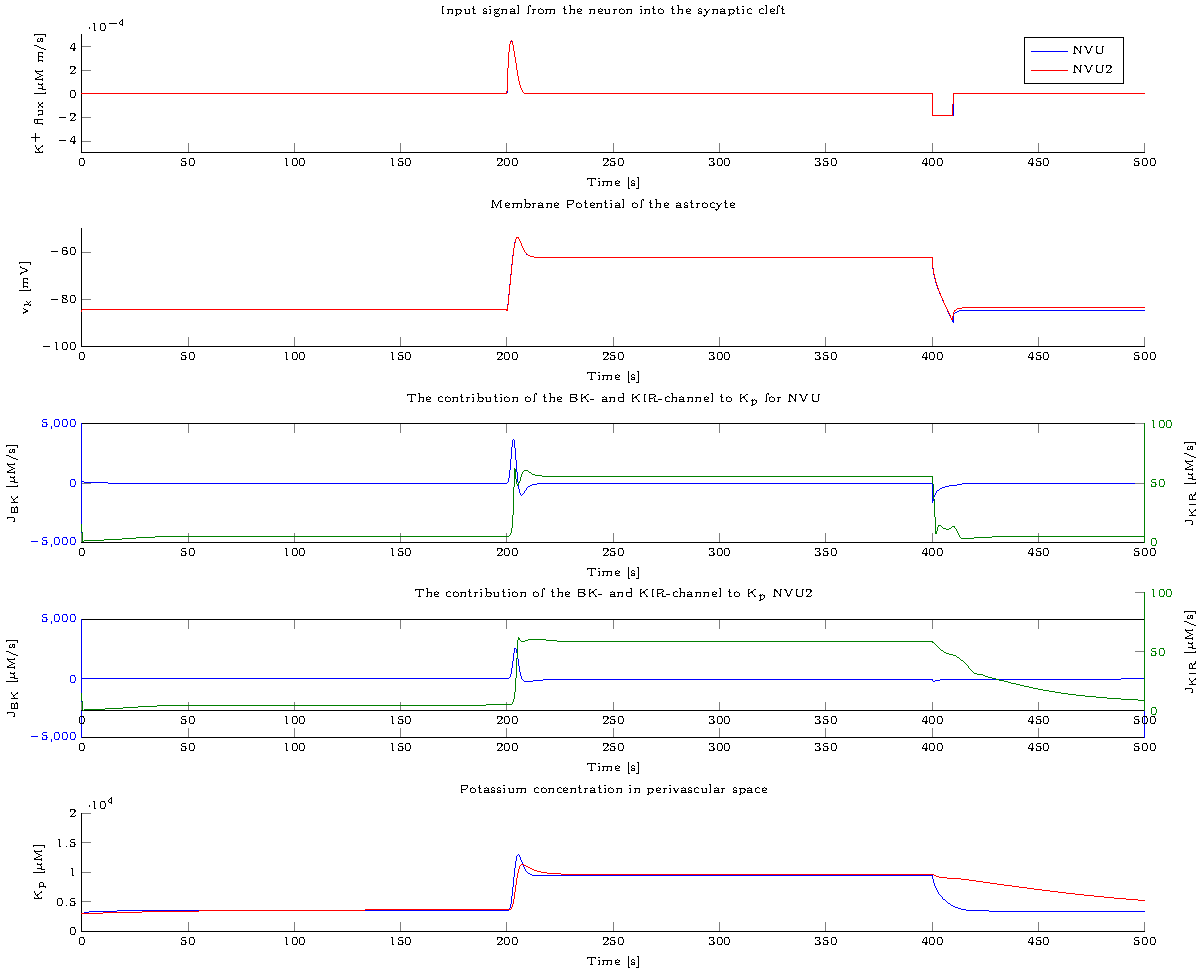
\includegraphics{figures/fig1_NVU_12.pdf}
		\caption{Overview 1, differences between NVU 1.1  \& 1.0}
		\label{fig:NVU10a}
	\end{figure}
	
	\begin{figure}[h!]
		\centering
		\tiny 
		\setlength\figureheight{2.5 cm} 
		\setlength\figurewidth{9 cm}
		%% % This file was created by matlab2tikz v0.3.3.
% Copyright (c) 2008--2013, Nico Schlömer <nico.schloemer@gmail.com>
% All rights reserved.
% 
% The latest updates can be retrieved from
%   http://www.mathworks.com/matlabcentral/fileexchange/22022-matlab2tikz
% where you can also make suggestions and rate matlab2tikz.
% 
% 
% 
\tiny 
\newlength\figureheight 
\newlength\figurewidth 
\setlength\figureheight{2.5 cm} 
\setlength\figurewidth{9 cm}

\begin{tikzpicture}

\begin{axis}[%
width=\figurewidth,
height=\figureheight,
scale only axis,
xmin=0,
xmax=600,
xlabel={Time [s]},
ymin=0,
ymax=20,
ylabel={$\text{[K}^\text{+}\text{]}_\text{s}\text{ [mM]}$},
name=plot3,
title={$\text{[K}^\text{+}\text{] in perivascular space}$},
axis x line*=bottom,
axis y line*=left
]
\addplot [
color=blue,
solid,
forget plot
]
table[row sep=crcr]{
0 3\\
0.00089136 3.0001\\
0.0017827 3.0002\\
0.0026741 3.0003\\
0.0061751 3.0008\\
0.0096762 3.0012\\
0.013177 3.0017\\
0.016678 3.0021\\
0.026472 3.0034\\
0.036266 3.0047\\
0.04606 3.006\\
0.055854 3.0072\\
0.065648 3.0085\\
0.075699 3.0098\\
0.079199 3.0103\\
0.0827 3.0108\\
0.086201 3.0112\\
0.089702 3.0117\\
0.093202 3.0121\\
0.10095 3.0131\\
0.1087 3.0142\\
0.11645 3.0152\\
0.12421 3.0162\\
0.14151 3.0184\\
0.15881 3.0206\\
0.17612 3.0229\\
0.19342 3.0251\\
0.21073 3.0273\\
0.2497 3.0322\\
0.28868 3.037\\
0.32765 3.0417\\
0.36662 3.0463\\
0.37628 3.0475\\
0.38594 3.0486\\
0.39561 3.0497\\
0.40527 3.0508\\
0.41493 3.052\\
0.43002 3.0537\\
0.44221 3.0551\\
0.4544 3.0565\\
0.46659 3.0579\\
0.47879 3.0592\\
0.49098 3.0606\\
0.51139 3.0629\\
0.52695 3.0647\\
0.54251 3.0664\\
0.55807 3.0681\\
0.57363 3.0698\\
0.58919 3.0715\\
0.6088 3.0737\\
0.6284 3.0758\\
0.64801 3.0779\\
0.66761 3.08\\
0.68722 3.0821\\
0.73766 3.0874\\
0.78811 3.0926\\
0.83855 3.0977\\
0.889 3.1028\\
0.93944 3.1078\\
1.0031 3.114\\
1.0667 3.12\\
1.1303 3.1259\\
1.1939 3.1318\\
1.2576 3.1375\\
1.3769 3.1479\\
1.4783 3.1564\\
1.5797 3.1647\\
1.6811 3.1728\\
1.7825 3.1806\\
1.8839 3.1882\\
2.0684 3.2014\\
2.2528 3.2139\\
2.4373 3.2257\\
2.6218 3.2369\\
2.8063 3.2475\\
2.9907 3.2576\\
3.3424 3.2754\\
3.694 3.2914\\
4.0456 3.306\\
4.3972 3.3192\\
4.7489 3.3311\\
5.2238 3.3455\\
5.6986 3.3581\\
6.1735 3.3692\\
6.6484 3.379\\
7.1233 3.3875\\
7.8241 3.3984\\
8.525 3.4073\\
9.2258 3.4148\\
9.9266 3.4209\\
10.627 3.4261\\
11.627 3.432\\
12.627 3.4366\\
13.627 3.4402\\
14.627 3.443\\
15.627 3.4453\\
16.627 3.4471\\
17.627 3.4486\\
18.627 3.4498\\
19.627 3.4509\\
20.627 3.4518\\
21.627 3.4526\\
22.627 3.4534\\
23.627 3.4541\\
24.627 3.4547\\
25.627 3.4553\\
26.627 3.4558\\
27.627 3.4564\\
28.627 3.4569\\
29.627 3.4573\\
30.627 3.4578\\
31.627 3.4582\\
32.627 3.4586\\
33.627 3.459\\
34.627 3.4593\\
35.627 3.4597\\
36.627 3.46\\
37.627 3.4603\\
38.627 3.4606\\
39.627 3.4609\\
40.627 3.4611\\
41.627 3.4614\\
42.627 3.4616\\
43.627 3.4618\\
44.627 3.462\\
45.627 3.4621\\
46.627 3.4622\\
47.627 3.4622\\
48.627 3.4623\\
49.627 3.4623\\
50.627 3.4622\\
51.627 3.4622\\
52.627 3.4621\\
53.627 3.4621\\
54.627 3.462\\
55.627 3.462\\
56.627 3.4619\\
57.627 3.4619\\
58.627 3.4619\\
59.627 3.4619\\
60.627 3.4619\\
61.627 3.4619\\
62.627 3.4619\\
63.627 3.4619\\
64.627 3.4619\\
65.627 3.4619\\
66.627 3.462\\
67.627 3.462\\
68.627 3.462\\
69.627 3.462\\
70.627 3.462\\
71.627 3.462\\
72.627 3.462\\
73.627 3.4621\\
74.627 3.4621\\
75.627 3.4621\\
76.627 3.4621\\
77.627 3.4621\\
78.627 3.4621\\
79.627 3.462\\
80.627 3.462\\
81.627 3.462\\
82.627 3.462\\
83.627 3.462\\
84.627 3.462\\
85.627 3.462\\
86.627 3.462\\
87.627 3.462\\
88.627 3.462\\
89.627 3.462\\
90.627 3.462\\
91.627 3.462\\
92.627 3.462\\
93.627 3.462\\
94.627 3.462\\
95.627 3.462\\
96.627 3.462\\
97.627 3.462\\
98.627 3.462\\
99.627 3.462\\
100.63 3.462\\
101.63 3.462\\
102.63 3.462\\
103.63 3.462\\
104.63 3.462\\
105.63 3.462\\
106.63 3.462\\
107.63 3.462\\
108.63 3.462\\
109.63 3.462\\
110.63 3.462\\
111.63 3.462\\
112.63 3.462\\
113.63 3.462\\
114.63 3.462\\
115.63 3.462\\
116.63 3.462\\
117.63 3.462\\
118.63 3.462\\
119.63 3.462\\
120.63 3.462\\
121.63 3.462\\
122.63 3.462\\
123.63 3.462\\
124.63 3.462\\
125.63 3.462\\
126.63 3.462\\
127.63 3.462\\
128.63 3.462\\
129.63 3.462\\
130.63 3.462\\
131.63 3.462\\
132.63 3.462\\
133.63 3.462\\
134.63 3.462\\
135.63 3.462\\
136.63 3.462\\
137.63 3.462\\
138.63 3.462\\
139.63 3.462\\
140.63 3.462\\
141.63 3.462\\
142.63 3.462\\
143.63 3.462\\
144.63 3.462\\
145.63 3.462\\
146.63 3.462\\
147.63 3.462\\
148.63 3.462\\
149.63 3.462\\
150.63 3.462\\
151.63 3.462\\
152.63 3.462\\
153.63 3.462\\
154.63 3.462\\
155.63 3.462\\
156.63 3.462\\
157.63 3.462\\
158.63 3.462\\
159.63 3.462\\
160.63 3.462\\
161.63 3.462\\
162.63 3.462\\
163.63 3.462\\
164.63 3.462\\
165.63 3.462\\
166.63 3.462\\
167.63 3.462\\
168.63 3.462\\
169.63 3.462\\
170.63 3.462\\
171.63 3.462\\
172.63 3.462\\
173.63 3.462\\
174.63 3.462\\
175.63 3.462\\
176.63 3.462\\
177.63 3.462\\
178.63 3.462\\
179.63 3.462\\
180.63 3.462\\
181.63 3.462\\
182.63 3.462\\
183.63 3.462\\
184.63 3.462\\
185.63 3.462\\
186.63 3.462\\
187.63 3.462\\
188.63 3.462\\
189.63 3.462\\
190.63 3.462\\
191.63 3.462\\
192.63 3.462\\
193.63 3.462\\
194.63 3.462\\
195.63 3.462\\
196.63 3.462\\
197.19 3.462\\
197.62 3.462\\
197.92 3.462\\
198.17 3.462\\
198.37 3.462\\
198.57 3.462\\
198.71 3.462\\
198.85 3.462\\
198.97 3.462\\
199.09 3.462\\
199.21 3.462\\
199.4 3.462\\
199.6 3.462\\
199.8 3.462\\
199.99 3.462\\
200.31 3.4705\\
200.54 3.4929\\
200.77 3.5447\\
201.01 3.6411\\
201.24 3.7974\\
201.54 4.1098\\
201.84 4.5822\\
202.14 5.2439\\
202.43 6.0987\\
202.73 7.109\\
203.03 8.2093\\
203.33 9.319\\
203.42 9.6413\\
203.51 9.9545\\
203.6 10.257\\
203.69 10.546\\
203.78 10.82\\
203.89 11.148\\
204 11.448\\
204.12 11.721\\
204.23 11.965\\
204.34 12.181\\
204.53 12.468\\
204.71 12.684\\
204.89 12.834\\
205.08 12.921\\
205.45 12.941\\
205.83 12.784\\
206.2 12.506\\
206.58 12.162\\
207.23 11.522\\
207.87 10.942\\
208.52 10.481\\
209.17 10.149\\
209.82 9.9179\\
210.52 9.7429\\
211.23 9.6238\\
211.93 9.5454\\
212.64 9.4948\\
213.34 9.4617\\
214.34 9.4329\\
215.34 9.4163\\
216.34 9.4068\\
217.34 9.4017\\
218.34 9.3988\\
219.34 9.3972\\
220.34 9.3962\\
221.34 9.3957\\
222.34 9.3955\\
223.34 9.3953\\
224.34 9.3952\\
225.34 9.3952\\
226.34 9.3952\\
227.34 9.3952\\
228.34 9.3952\\
229.34 9.3952\\
230.34 9.3952\\
231.34 9.3951\\
232.34 9.3951\\
233.34 9.3951\\
234.34 9.3951\\
235.34 9.3951\\
236.34 9.3951\\
237.34 9.3951\\
238.34 9.3951\\
239.34 9.3951\\
240.34 9.3951\\
241.34 9.3951\\
242.34 9.3951\\
243.34 9.3951\\
244.34 9.3951\\
245.34 9.3951\\
246.34 9.3951\\
247.34 9.3951\\
248.34 9.3951\\
249.34 9.3951\\
250.34 9.3951\\
251.34 9.3951\\
252.34 9.3951\\
253.34 9.3951\\
254.34 9.3951\\
255.34 9.3951\\
256.34 9.3951\\
257.34 9.3951\\
258.34 9.3951\\
259.34 9.3951\\
260.34 9.3951\\
261.34 9.3951\\
262.34 9.3951\\
263.34 9.3951\\
264.34 9.3951\\
265.34 9.3951\\
266.34 9.3951\\
267.34 9.3951\\
268.34 9.3951\\
269.34 9.3951\\
270.34 9.3951\\
271.34 9.3951\\
272.34 9.3951\\
273.34 9.3951\\
274.34 9.3951\\
275.34 9.3951\\
276.34 9.3951\\
277.34 9.3951\\
278.34 9.3951\\
279.34 9.3951\\
280.34 9.3951\\
281.34 9.3951\\
282.34 9.3951\\
283.34 9.3951\\
284.34 9.3951\\
285.34 9.3951\\
286.34 9.3951\\
287.34 9.3951\\
288.34 9.3951\\
289.34 9.3951\\
290.34 9.3951\\
291.34 9.3951\\
292.34 9.3951\\
293.34 9.3951\\
294.34 9.3951\\
295.34 9.3951\\
296.34 9.3951\\
297.34 9.3951\\
298.34 9.3951\\
299.34 9.3951\\
300.34 9.3951\\
301.34 9.3951\\
302.34 9.3951\\
303.34 9.3951\\
304.34 9.3951\\
305.34 9.3951\\
306.34 9.3951\\
307.34 9.3951\\
308.34 9.3951\\
309.34 9.3951\\
310.34 9.3951\\
311.34 9.3951\\
312.34 9.3951\\
313.34 9.3951\\
314.34 9.3951\\
315.34 9.3951\\
316.34 9.3951\\
317.34 9.3951\\
318.34 9.3951\\
319.34 9.3951\\
320.34 9.3951\\
321.34 9.3951\\
322.34 9.3951\\
323.34 9.3951\\
324.34 9.3951\\
325.34 9.3951\\
326.34 9.3951\\
327.34 9.3951\\
328.34 9.3951\\
329.34 9.3951\\
330.34 9.3951\\
331.34 9.3951\\
332.34 9.3951\\
333.34 9.3951\\
334.34 9.3951\\
335.34 9.3951\\
336.34 9.3951\\
337.34 9.3951\\
338.34 9.3951\\
339.34 9.3951\\
340.34 9.3951\\
341.34 9.3951\\
342.34 9.3951\\
343.34 9.3951\\
344.34 9.3951\\
345.34 9.3951\\
346.34 9.3951\\
347.34 9.3951\\
348.34 9.3951\\
349.34 9.3951\\
350.34 9.3951\\
351.34 9.3951\\
352.34 9.3951\\
353.34 9.3951\\
354.34 9.3951\\
355.34 9.3951\\
356.34 9.3951\\
357.34 9.3951\\
358.34 9.3951\\
359.34 9.3951\\
360.34 9.3951\\
361.34 9.3951\\
362.34 9.3951\\
363.34 9.3951\\
364.34 9.3951\\
365.34 9.3951\\
366.34 9.3951\\
367.34 9.3951\\
368.34 9.3951\\
369.34 9.3951\\
370.34 9.3951\\
371.34 9.3951\\
372.34 9.3951\\
373.34 9.3951\\
374.34 9.3951\\
375.34 9.3951\\
376.34 9.3951\\
377.34 9.3951\\
378.34 9.3951\\
379.34 9.3951\\
380.34 9.3951\\
381.34 9.3951\\
382.34 9.3951\\
383.34 9.3951\\
384.34 9.3951\\
385.34 9.3951\\
386.34 9.3951\\
387.34 9.3951\\
388.34 9.3951\\
389.34 9.3951\\
390.34 9.3951\\
391.34 9.3951\\
392.34 9.3951\\
393.34 9.3951\\
394.34 9.3951\\
395.34 9.3951\\
396.34 9.3951\\
397.34 9.3951\\
398.17 9.3951\\
398.58 9.3951\\
398.9 9.3951\\
399.16 9.3951\\
399.42 9.3951\\
399.62 9.3951\\
399.82 9.3951\\
399.88 9.3951\\
399.94 9.3951\\
399.99 9.3951\\
400.03 9.3721\\
400.08 9.3308\\
400.15 9.2401\\
400.22 9.1317\\
400.29 9.0181\\
400.36 8.9068\\
400.48 8.7364\\
400.59 8.5785\\
400.71 8.4313\\
400.83 8.2925\\
401.11 7.9862\\
401.23 7.8582\\
401.33 7.76\\
401.41 7.6831\\
401.5 7.6083\\
401.56 7.5491\\
401.63 7.4912\\
401.66 7.4605\\
401.69 7.4363\\
401.72 7.4122\\
401.75 7.3884\\
401.78 7.3648\\
401.81 7.3339\\
401.85 7.3033\\
401.89 7.2732\\
401.93 7.2434\\
401.98 7.2016\\
402.03 7.1605\\
402.09 7.12\\
402.14 7.0803\\
402.2 7.0413\\
402.37 6.916\\
402.55 6.7973\\
402.68 6.7162\\
402.81 6.638\\
402.93 6.5625\\
403.06 6.4894\\
403.27 6.3726\\
403.44 6.2854\\
403.6 6.2015\\
403.77 6.1205\\
403.93 6.0424\\
404.15 5.9428\\
404.37 5.8474\\
404.59 5.7559\\
404.81 5.668\\
405.2 5.5209\\
405.58 5.3832\\
405.97 5.2539\\
406.36 5.1321\\
406.74 5.0174\\
407.4 4.8361\\
408.07 4.6715\\
408.61 4.547\\
409.16 4.4321\\
409.32 4.3993\\
409.48 4.3674\\
409.65 4.3363\\
409.81 4.3058\\
409.97 4.2761\\
410.14 4.2479\\
410.3 4.2217\\
410.47 4.1932\\
410.63 4.1616\\
410.8 4.1308\\
410.96 4.1029\\
411.13 4.0763\\
411.38 4.0368\\
411.64 3.9983\\
411.89 3.9623\\
412.14 3.9288\\
412.4 3.8972\\
412.65 3.8673\\
413.05 3.8244\\
413.31 3.798\\
413.53 3.7779\\
413.72 3.7605\\
413.89 3.7461\\
414.02 3.7355\\
414.15 3.7252\\
414.28 3.7153\\
414.41 3.7057\\
414.63 3.6907\\
414.85 3.6766\\
415.07 3.6633\\
415.47 3.6402\\
415.87 3.6194\\
416.28 3.6007\\
416.68 3.5839\\
417.45 3.5565\\
418.22 3.5342\\
418.99 3.516\\
419.75 3.5012\\
420.75 3.4859\\
421.75 3.4743\\
422.75 3.4654\\
423.75 3.4587\\
424.75 3.4537\\
425.75 3.4499\\
426.75 3.4471\\
427.75 3.445\\
428.75 3.4435\\
429.75 3.4425\\
430.75 3.4417\\
431.75 3.4412\\
432.75 3.4408\\
433.75 3.4406\\
434.75 3.4404\\
435.75 3.4403\\
436.75 3.4402\\
437.75 3.4402\\
438.75 3.4401\\
439.75 3.4401\\
440.75 3.4401\\
441.75 3.4401\\
442.75 3.44\\
443.75 3.44\\
444.75 3.44\\
445.75 3.4399\\
446.75 3.4399\\
447.75 3.4399\\
448.75 3.4399\\
449.75 3.4399\\
450.75 3.4399\\
451.75 3.4398\\
452.75 3.4398\\
453.75 3.4398\\
454.75 3.4398\\
455.75 3.4398\\
456.75 3.4398\\
457.75 3.4398\\
458.75 3.4398\\
459.75 3.4398\\
460.75 3.4399\\
461.75 3.4399\\
462.75 3.4399\\
463.75 3.4399\\
464.75 3.4399\\
465.75 3.4399\\
466.75 3.4399\\
467.75 3.4399\\
468.75 3.4399\\
469.75 3.4399\\
470.75 3.4399\\
471.75 3.4399\\
472.75 3.4399\\
473.75 3.4399\\
474.75 3.4399\\
475.75 3.4399\\
476.75 3.4399\\
477.75 3.4399\\
478.75 3.4399\\
479.75 3.4399\\
480.75 3.4399\\
481.75 3.4399\\
482.75 3.4399\\
483.75 3.4399\\
484.75 3.4399\\
485.75 3.4399\\
486.75 3.4399\\
487.75 3.4399\\
488.75 3.4399\\
489.75 3.4399\\
490.75 3.4399\\
491.75 3.4399\\
492.75 3.4399\\
493.75 3.4399\\
494.75 3.4399\\
495.75 3.4399\\
496.75 3.4399\\
497.75 3.4399\\
498.75 3.4399\\
499.75 3.4399\\
500 3.4399\\
};
\addplot [
color=red,
solid,
forget plot
]
table[row sep=crcr]{
0 3\\
0.0011996 3.0002\\
0.0023992 3.0003\\
0.0035988 3.0004\\
0.0085566 3.001\\
0.013514 3.0015\\
0.018472 3.002\\
0.02343 3.0025\\
0.033542 3.0033\\
0.043655 3.004\\
0.053767 3.0046\\
0.063879 3.0052\\
0.073991 3.0056\\
0.084819 3.0061\\
0.095647 3.0065\\
0.10647 3.0068\\
0.1173 3.0071\\
0.12813 3.0074\\
0.14659 3.0079\\
0.16505 3.0083\\
0.18351 3.0086\\
0.20197 3.009\\
0.22042 3.0093\\
0.26398 3.0099\\
0.30753 3.0106\\
0.35108 3.0111\\
0.37397 3.0114\\
0.38969 3.0116\\
0.4054 3.0118\\
0.42111 3.012\\
0.43393 3.0121\\
0.44676 3.0123\\
0.45959 3.0124\\
0.47242 3.0125\\
0.48525 3.0127\\
0.50035 3.0129\\
0.51544 3.013\\
0.53054 3.0132\\
0.54564 3.0134\\
0.56073 3.0135\\
0.57728 3.0137\\
0.59382 3.0139\\
0.61036 3.0141\\
0.6269 3.0143\\
0.64344 3.0144\\
0.65998 3.0146\\
0.69992 3.0151\\
0.73986 3.0155\\
0.77979 3.016\\
0.81973 3.0164\\
0.85967 3.0168\\
0.99616 3.0184\\
1.1327 3.0199\\
1.2692 3.0214\\
1.4056 3.0229\\
1.6062 3.0251\\
1.8067 3.0273\\
2.0072 3.0296\\
2.2078 3.0318\\
2.4083 3.034\\
2.8551 3.0388\\
3.302 3.0436\\
3.7488 3.0484\\
4.1956 3.0531\\
4.6425 3.0578\\
5.3586 3.0651\\
6.0748 3.0724\\
6.791 3.0796\\
7.5072 3.0866\\
8.2234 3.0936\\
9.2234 3.1032\\
10.223 3.1126\\
11.223 3.1218\\
12.223 3.1309\\
12.523 3.1336\\
12.823 3.1362\\
13.123 3.1389\\
13.423 3.1416\\
13.513 3.1424\\
13.603 3.1431\\
13.693 3.1439\\
13.783 3.1447\\
13.873 3.1455\\
13.929 3.146\\
13.948 3.1462\\
13.967 3.1463\\
13.986 3.1465\\
14.004 3.1466\\
14.023 3.1468\\
14.079 3.1473\\
14.134 3.1478\\
14.189 3.1483\\
14.244 3.1488\\
14.299 3.1493\\
14.354 3.1497\\
14.409 3.1501\\
14.465 3.1506\\
14.52 3.151\\
14.575 3.1516\\
14.631 3.1522\\
14.686 3.153\\
14.742 3.1538\\
14.811 3.1551\\
14.88 3.1564\\
14.95 3.1578\\
15.019 3.1593\\
15.089 3.1608\\
15.202 3.1632\\
15.315 3.1654\\
15.428 3.1675\\
15.541 3.1694\\
15.654 3.1711\\
15.804 3.1732\\
15.954 3.1751\\
16.104 3.1769\\
16.255 3.1785\\
16.405 3.1801\\
16.675 3.1831\\
16.946 3.1861\\
17.216 3.1891\\
17.487 3.1919\\
17.757 3.1945\\
18.061 3.1973\\
18.364 3.1999\\
18.667 3.2024\\
18.971 3.2049\\
19.274 3.2073\\
19.375 3.2081\\
19.476 3.2089\\
19.576 3.2097\\
19.677 3.2105\\
19.778 3.2112\\
19.938 3.2125\\
20.097 3.2137\\
20.257 3.215\\
20.416 3.2162\\
20.576 3.2174\\
20.994 3.2207\\
21.411 3.2239\\
21.828 3.2271\\
22.056 3.2288\\
22.119 3.2293\\
22.183 3.2298\\
22.247 3.2303\\
22.31 3.2308\\
22.432 3.2317\\
22.554 3.2326\\
22.676 3.2336\\
22.798 3.2345\\
22.92 3.2355\\
23.367 3.239\\
23.684 3.2415\\
24 3.244\\
24.242 3.246\\
24.484 3.248\\
24.726 3.25\\
24.968 3.252\\
25.298 3.2547\\
25.628 3.2574\\
25.958 3.2602\\
26.288 3.2629\\
26.618 3.2656\\
27.087 3.2693\\
27.556 3.273\\
28.025 3.2767\\
28.494 3.2803\\
28.964 3.2839\\
29.615 3.2888\\
30.266 3.2936\\
30.917 3.2984\\
31.569 3.3032\\
32.372 3.309\\
33.175 3.3148\\
33.979 3.3206\\
34.782 3.3263\\
35.586 3.332\\
36.23 3.3365\\
36.875 3.3409\\
37.52 3.3453\\
38.164 3.3497\\
38.969 3.3551\\
39.774 3.3604\\
40.579 3.3656\\
41.384 3.3708\\
42.189 3.3759\\
43.189 3.3821\\
44.189 3.3882\\
45.189 3.3942\\
46.189 3.4001\\
47.189 3.4058\\
48.189 3.4114\\
49.189 3.4168\\
50.189 3.422\\
51.189 3.4271\\
52.189 3.4321\\
53.189 3.4369\\
54.189 3.4417\\
55.189 3.4463\\
56.189 3.4507\\
57.189 3.4551\\
58.189 3.4594\\
59.189 3.4636\\
60.189 3.4677\\
61.189 3.4718\\
62.189 3.4757\\
63.189 3.4796\\
64.189 3.4834\\
65.189 3.4871\\
66.189 3.4907\\
67.189 3.4943\\
68.189 3.4978\\
69.189 3.5011\\
70.189 3.5045\\
71.189 3.5077\\
72.189 3.5109\\
73.189 3.514\\
74.189 3.5171\\
75.189 3.5201\\
76.189 3.523\\
77.189 3.5258\\
78.189 3.5286\\
79.189 3.5313\\
80.189 3.5339\\
81.189 3.5365\\
82.189 3.5391\\
83.189 3.5416\\
84.189 3.544\\
85.189 3.5464\\
86.189 3.5487\\
87.189 3.551\\
88.189 3.5532\\
89.189 3.5554\\
90.189 3.5575\\
91.189 3.5596\\
92.189 3.5616\\
93.189 3.5636\\
94.189 3.5656\\
95.189 3.5675\\
96.189 3.5693\\
97.189 3.5712\\
98.189 3.573\\
99.189 3.5747\\
100.19 3.5764\\
101.19 3.5781\\
102.19 3.5797\\
103.19 3.5814\\
104.19 3.5829\\
105.19 3.5845\\
106.19 3.586\\
107.19 3.5874\\
108.19 3.5889\\
109.19 3.5903\\
110.19 3.5917\\
111.19 3.593\\
112.19 3.5944\\
113.19 3.5956\\
114.19 3.5969\\
115.19 3.5982\\
116.19 3.5994\\
117.19 3.6006\\
118.19 3.6017\\
119.19 3.6029\\
120.19 3.604\\
121.19 3.6051\\
122.19 3.6061\\
123.19 3.6072\\
124.19 3.6082\\
125.19 3.6092\\
126.19 3.6102\\
127.19 3.6111\\
128.19 3.6121\\
129.19 3.613\\
130.19 3.6139\\
131.19 3.6148\\
132.19 3.6156\\
133.19 3.6165\\
134.19 3.6173\\
135.19 3.6181\\
136.19 3.6189\\
137.19 3.6197\\
138.19 3.6205\\
139.19 3.6212\\
140.19 3.6219\\
141.19 3.6226\\
142.19 3.6233\\
143.19 3.624\\
144.19 3.6247\\
145.19 3.6253\\
146.19 3.626\\
147.19 3.6266\\
148.19 3.6272\\
149.19 3.6278\\
150.19 3.6284\\
151.19 3.629\\
152.19 3.6295\\
153.19 3.6301\\
154.19 3.6306\\
155.19 3.6312\\
156.19 3.6317\\
157.19 3.6322\\
158.19 3.6327\\
159.19 3.6332\\
160.19 3.6336\\
161.19 3.6341\\
162.19 3.6346\\
163.19 3.635\\
164.19 3.6354\\
165.19 3.6359\\
166.19 3.6363\\
167.19 3.6367\\
168.19 3.6371\\
169.19 3.6375\\
170.19 3.6379\\
171.19 3.6383\\
172.19 3.6386\\
173.19 3.639\\
174.19 3.6393\\
175.19 3.6397\\
176.19 3.64\\
177.19 3.6404\\
178.19 3.6407\\
179.19 3.641\\
180.19 3.6413\\
181.19 3.6416\\
182.19 3.6419\\
183.19 3.6422\\
184.19 3.6425\\
185.19 3.6428\\
186.19 3.643\\
187.19 3.6433\\
188.19 3.6436\\
189.19 3.6438\\
190.19 3.6441\\
191.19 3.6443\\
192.19 3.6446\\
193.19 3.6448\\
194.19 3.645\\
195.19 3.6453\\
196.19 3.6455\\
196.81 3.6456\\
197.25 3.6457\\
197.57 3.6458\\
197.82 3.6458\\
198.03 3.6459\\
198.24 3.6459\\
198.38 3.6459\\
198.52 3.646\\
198.63 3.646\\
198.74 3.646\\
198.83 3.646\\
198.92 3.646\\
199.01 3.646\\
199.17 3.646\\
199.32 3.646\\
199.47 3.646\\
199.62 3.646\\
199.84 3.646\\
200.07 3.6457\\
200.29 3.6457\\
200.51 3.6471\\
200.69 3.6503\\
200.87 3.6559\\
201.05 3.6652\\
201.23 3.6798\\
201.42 3.7023\\
201.6 3.7364\\
201.79 3.7857\\
201.97 3.8557\\
202.15 3.9532\\
202.34 4.0856\\
202.63 4.3805\\
202.92 4.7972\\
203.21 5.3395\\
203.5 5.9916\\
203.79 6.7189\\
204.09 7.5047\\
204.39 8.2733\\
204.69 8.9844\\
204.94 9.5062\\
205.19 9.9615\\
205.44 10.344\\
205.68 10.654\\
205.85 10.825\\
206.02 10.965\\
206.19 11.079\\
206.36 11.167\\
206.6 11.257\\
206.84 11.312\\
207.08 11.338\\
207.32 11.341\\
207.65 11.319\\
207.99 11.276\\
208.32 11.219\\
208.65 11.155\\
208.99 11.088\\
209.66 10.948\\
210.18 10.845\\
210.7 10.747\\
211.22 10.655\\
211.74 10.568\\
212.26 10.488\\
212.9 10.396\\
213.54 10.311\\
214.18 10.235\\
214.82 10.167\\
215.46 10.106\\
216.16 10.048\\
216.87 9.9977\\
217.57 9.9541\\
218.27 9.9159\\
218.98 9.882\\
219.98 9.8399\\
220.98 9.8039\\
221.98 9.774\\
222.98 9.7505\\
223.98 9.7327\\
224.98 9.7185\\
225.98 9.7066\\
226.98 9.6962\\
227.98 9.687\\
228.98 9.6793\\
229.98 9.6733\\
230.98 9.6687\\
231.98 9.665\\
232.98 9.6619\\
233.98 9.659\\
234.98 9.6565\\
235.98 9.6547\\
236.98 9.6528\\
237.98 9.6519\\
238.98 9.651\\
239.98 9.6502\\
240.98 9.6495\\
241.98 9.649\\
242.98 9.6484\\
243.98 9.648\\
244.98 9.6476\\
245.98 9.6473\\
246.98 9.6471\\
247.98 9.6469\\
248.98 9.6467\\
249.98 9.6466\\
250.98 9.6465\\
251.98 9.6464\\
252.98 9.6464\\
253.98 9.6463\\
254.98 9.6462\\
255.98 9.6462\\
256.98 9.6462\\
257.98 9.6461\\
258.98 9.6461\\
259.98 9.6461\\
260.98 9.6461\\
261.98 9.6461\\
262.98 9.6461\\
263.98 9.646\\
264.98 9.646\\
265.98 9.646\\
266.98 9.646\\
267.98 9.646\\
268.98 9.646\\
269.98 9.646\\
270.98 9.646\\
271.98 9.646\\
272.98 9.646\\
273.98 9.646\\
274.98 9.646\\
275.98 9.646\\
276.98 9.646\\
277.98 9.646\\
278.98 9.646\\
279.98 9.646\\
280.98 9.646\\
281.98 9.646\\
282.98 9.646\\
283.98 9.646\\
284.98 9.646\\
285.98 9.646\\
286.98 9.646\\
287.98 9.646\\
288.98 9.646\\
289.98 9.646\\
290.98 9.646\\
291.98 9.646\\
292.98 9.646\\
293.98 9.646\\
294.98 9.646\\
295.98 9.646\\
296.98 9.646\\
297.98 9.646\\
298.98 9.646\\
299.98 9.646\\
300.98 9.646\\
301.98 9.646\\
302.98 9.646\\
303.98 9.646\\
304.98 9.646\\
305.98 9.646\\
306.98 9.646\\
307.98 9.646\\
308.98 9.646\\
309.98 9.646\\
310.98 9.646\\
311.98 9.646\\
312.98 9.646\\
313.98 9.6459\\
314.98 9.6459\\
315.98 9.6459\\
316.98 9.6459\\
317.98 9.6459\\
318.98 9.6459\\
319.98 9.6459\\
320.98 9.6459\\
321.98 9.6459\\
322.98 9.6459\\
323.98 9.6459\\
324.98 9.6459\\
325.98 9.6459\\
326.98 9.6459\\
327.98 9.6459\\
328.98 9.6459\\
329.98 9.6459\\
330.98 9.6459\\
331.98 9.6459\\
332.98 9.6459\\
333.98 9.6459\\
334.98 9.6459\\
335.98 9.6459\\
336.98 9.6459\\
337.98 9.6459\\
338.98 9.6459\\
339.98 9.6459\\
340.98 9.6459\\
341.98 9.6459\\
342.98 9.6459\\
343.98 9.6459\\
344.98 9.6459\\
345.98 9.6459\\
346.98 9.6459\\
347.98 9.6459\\
348.98 9.6459\\
349.98 9.6459\\
350.98 9.6459\\
351.98 9.6459\\
352.98 9.6459\\
353.98 9.6459\\
354.98 9.6459\\
355.98 9.6459\\
356.98 9.6459\\
357.98 9.6459\\
358.98 9.6459\\
359.98 9.6459\\
360.98 9.6459\\
361.98 9.6459\\
362.98 9.6459\\
363.98 9.6459\\
364.98 9.6459\\
365.98 9.6459\\
366.98 9.6459\\
367.98 9.6459\\
368.98 9.6459\\
369.98 9.6459\\
370.98 9.6459\\
371.98 9.6459\\
372.98 9.6459\\
373.98 9.6459\\
374.98 9.6459\\
375.98 9.6459\\
376.98 9.6459\\
377.98 9.6459\\
378.98 9.6459\\
379.98 9.6459\\
380.98 9.6459\\
381.98 9.6459\\
382.98 9.6459\\
383.98 9.6459\\
384.98 9.6459\\
385.98 9.6459\\
386.98 9.6459\\
387.98 9.6459\\
388.98 9.6459\\
389.98 9.6459\\
390.98 9.6459\\
391.98 9.6459\\
392.98 9.6459\\
393.98 9.6459\\
394.98 9.6459\\
395.98 9.6459\\
396.98 9.6459\\
397.98 9.6461\\
398.44 9.6461\\
398.8 9.6462\\
399.07 9.6462\\
399.35 9.6462\\
399.55 9.6462\\
399.76 9.6461\\
399.96 9.6461\\
400.26 9.6208\\
400.34 9.6069\\
400.43 9.5914\\
400.52 9.5753\\
400.61 9.5593\\
400.92 9.5046\\
401.24 9.453\\
401.56 9.4044\\
401.87 9.3594\\
402.11 9.328\\
402.35 9.299\\
402.59 9.2724\\
402.83 9.248\\
403.14 9.2193\\
403.45 9.1935\\
403.77 9.1705\\
404.08 9.1498\\
404.39 9.1312\\
404.93 9.103\\
405.47 9.079\\
406.02 9.0583\\
406.56 9.0409\\
407.1 9.0273\\
408.1 9.0087\\
408.77 9.0006\\
409.43 8.9956\\
410.1 8.9861\\
410.61 8.972\\
411.12 8.954\\
411.63 8.9349\\
412.15 8.9149\\
412.66 8.8942\\
413.31 8.8678\\
413.95 8.8412\\
414.6 8.8141\\
415.25 8.7863\\
415.9 8.7578\\
416.77 8.7178\\
417.65 8.6763\\
418.52 8.6332\\
419.4 8.5888\\
420.28 8.5436\\
421.2 8.4959\\
422.12 8.4486\\
423.04 8.402\\
423.96 8.3558\\
424.89 8.3094\\
425.81 8.2626\\
426.73 8.2156\\
427.68 8.1671\\
428.64 8.1187\\
429.59 8.0706\\
430.55 8.0225\\
431.5 7.9745\\
432.5 7.9243\\
433.5 7.8744\\
434.5 7.8247\\
435.5 7.7751\\
436.5 7.7256\\
437.5 7.6763\\
438.5 7.6271\\
439.5 7.5782\\
440.5 7.5295\\
441.5 7.4809\\
442.5 7.4326\\
443.5 7.3845\\
444.5 7.3367\\
445.5 7.289\\
446.5 7.2416\\
447.5 7.1945\\
448.5 7.1475\\
449.5 7.1008\\
450.5 7.0544\\
451.5 7.0082\\
452.5 6.9623\\
453.5 6.9167\\
454.5 6.8714\\
455.5 6.8265\\
456.5 6.7818\\
457.5 6.7375\\
458.5 6.6935\\
459.5 6.6499\\
460.5 6.6066\\
461.5 6.5637\\
462.5 6.5212\\
463.5 6.479\\
464.5 6.4373\\
465.5 6.3959\\
466.5 6.3549\\
467.5 6.3143\\
468.5 6.2741\\
469.5 6.2343\\
470.5 6.1949\\
471.5 6.1559\\
472.5 6.1174\\
473.5 6.0792\\
474.5 6.0415\\
475.5 6.0042\\
476.5 5.9673\\
477.5 5.9309\\
478.5 5.8949\\
479.5 5.8593\\
480.5 5.8241\\
481.5 5.7893\\
482.5 5.755\\
483.5 5.7212\\
484.5 5.6877\\
485.5 5.6547\\
486.5 5.6221\\
487.5 5.5899\\
488.5 5.5582\\
489.5 5.5268\\
490.5 5.4959\\
491.5 5.4655\\
492.5 5.4354\\
493.5 5.4058\\
494.5 5.3766\\
495.5 5.3478\\
496.5 5.3194\\
497.5 5.2915\\
498.5 5.2639\\
499.5 5.2367\\
500 5.2234\\
};
\end{axis}

\begin{axis}[%
width=\figurewidth,
height=\figureheight,
scale only axis,
xmin=0,
xmax=600,
xlabel={Time [s]},
ymin=0,
ymax=20,
ylabel={$\text{[K}^\text{+}\text{]}_\text{s}\text{ [mM]}$},
name=plot1,
at=(plot3.above north west),
anchor=below south west,
title={$\text{[K}^\text{+}\text{] in synaptic cleft}$},
axis x line*=bottom,
axis y line*=left,
legend style={draw=black,fill=white,legend cell align=left}
]
\addplot [
color=blue,
solid
]
table[row sep=crcr]{
0 3\\
0.00089136 2.9986\\
0.0017827 2.9999\\
0.0026741 3.0009\\
0.0061751 3.0046\\
0.0096762 3.0081\\
0.013177 3.0114\\
0.016678 3.0144\\
0.026472 3.0221\\
0.036266 3.0285\\
0.04606 3.0339\\
0.055854 3.0384\\
0.065648 3.0422\\
0.075699 3.0455\\
0.079199 3.0465\\
0.0827 3.0474\\
0.086201 3.0483\\
0.089702 3.0492\\
0.093202 3.0499\\
0.10095 3.0515\\
0.1087 3.0529\\
0.11645 3.0541\\
0.12421 3.0551\\
0.14151 3.057\\
0.15881 3.0583\\
0.17612 3.0593\\
0.19342 3.06\\
0.21073 3.0605\\
0.2497 3.0611\\
0.28868 3.0613\\
0.32765 3.0614\\
0.36662 3.0613\\
0.37628 3.0613\\
0.38594 3.0613\\
0.39561 3.0612\\
0.40527 3.0612\\
0.41493 3.0611\\
0.43002 3.0611\\
0.44221 3.061\\
0.4544 3.061\\
0.46659 3.0609\\
0.47879 3.0609\\
0.49098 3.0608\\
0.51139 3.0607\\
0.52695 3.0606\\
0.54251 3.0605\\
0.55807 3.0605\\
0.57363 3.0604\\
0.58919 3.0603\\
0.6088 3.0602\\
0.6284 3.0601\\
0.64801 3.06\\
0.66761 3.0599\\
0.68722 3.0598\\
0.73766 3.0595\\
0.78811 3.0593\\
0.83855 3.059\\
0.889 3.0588\\
0.93944 3.0585\\
1.0031 3.0582\\
1.0667 3.058\\
1.1303 3.0577\\
1.1939 3.0574\\
1.2576 3.0571\\
1.3769 3.0567\\
1.4783 3.0563\\
1.5797 3.056\\
1.6811 3.0557\\
1.7825 3.0554\\
1.8839 3.0551\\
2.0684 3.0546\\
2.2528 3.0542\\
2.4373 3.0539\\
2.6218 3.0536\\
2.8063 3.0533\\
2.9907 3.0531\\
3.3424 3.0527\\
3.694 3.0525\\
4.0456 3.0522\\
4.3972 3.0521\\
4.7489 3.0519\\
5.2238 3.0518\\
5.6986 3.0517\\
6.1735 3.0517\\
6.6484 3.0516\\
7.1233 3.0516\\
7.8241 3.0516\\
8.525 3.0515\\
9.2258 3.0515\\
9.9266 3.0515\\
10.627 3.0515\\
11.627 3.0515\\
12.627 3.0515\\
13.627 3.0515\\
14.627 3.0515\\
15.627 3.0515\\
16.627 3.0515\\
17.627 3.0515\\
18.627 3.0515\\
19.627 3.0515\\
20.627 3.0515\\
21.627 3.0515\\
22.627 3.0515\\
23.627 3.0515\\
24.627 3.0515\\
25.627 3.0515\\
26.627 3.0515\\
27.627 3.0515\\
28.627 3.0515\\
29.627 3.0515\\
30.627 3.0515\\
31.627 3.0515\\
32.627 3.0515\\
33.627 3.0515\\
34.627 3.0515\\
35.627 3.0515\\
36.627 3.0515\\
37.627 3.0515\\
38.627 3.0515\\
39.627 3.0515\\
40.627 3.0515\\
41.627 3.0515\\
42.627 3.0515\\
43.627 3.0515\\
44.627 3.0515\\
45.627 3.0515\\
46.627 3.0515\\
47.627 3.0515\\
48.627 3.0515\\
49.627 3.0515\\
50.627 3.0515\\
51.627 3.0515\\
52.627 3.0515\\
53.627 3.0515\\
54.627 3.0515\\
55.627 3.0515\\
56.627 3.0515\\
57.627 3.0515\\
58.627 3.0515\\
59.627 3.0515\\
60.627 3.0515\\
61.627 3.0515\\
62.627 3.0515\\
63.627 3.0515\\
64.627 3.0515\\
65.627 3.0515\\
66.627 3.0515\\
67.627 3.0515\\
68.627 3.0515\\
69.627 3.0515\\
70.627 3.0515\\
71.627 3.0515\\
72.627 3.0515\\
73.627 3.0515\\
74.627 3.0515\\
75.627 3.0515\\
76.627 3.0515\\
77.627 3.0515\\
78.627 3.0515\\
79.627 3.0515\\
80.627 3.0515\\
81.627 3.0515\\
82.627 3.0515\\
83.627 3.0515\\
84.627 3.0515\\
85.627 3.0515\\
86.627 3.0515\\
87.627 3.0515\\
88.627 3.0515\\
89.627 3.0515\\
90.627 3.0515\\
91.627 3.0515\\
92.627 3.0515\\
93.627 3.0515\\
94.627 3.0515\\
95.627 3.0515\\
96.627 3.0515\\
97.627 3.0515\\
98.627 3.0515\\
99.627 3.0515\\
100.63 3.0515\\
101.63 3.0515\\
102.63 3.0515\\
103.63 3.0515\\
104.63 3.0515\\
105.63 3.0515\\
106.63 3.0515\\
107.63 3.0515\\
108.63 3.0515\\
109.63 3.0515\\
110.63 3.0515\\
111.63 3.0515\\
112.63 3.0515\\
113.63 3.0515\\
114.63 3.0515\\
115.63 3.0515\\
116.63 3.0515\\
117.63 3.0515\\
118.63 3.0515\\
119.63 3.0515\\
120.63 3.0515\\
121.63 3.0515\\
122.63 3.0515\\
123.63 3.0515\\
124.63 3.0515\\
125.63 3.0515\\
126.63 3.0515\\
127.63 3.0515\\
128.63 3.0515\\
129.63 3.0515\\
130.63 3.0515\\
131.63 3.0515\\
132.63 3.0515\\
133.63 3.0515\\
134.63 3.0515\\
135.63 3.0515\\
136.63 3.0515\\
137.63 3.0515\\
138.63 3.0515\\
139.63 3.0515\\
140.63 3.0515\\
141.63 3.0515\\
142.63 3.0515\\
143.63 3.0515\\
144.63 3.0515\\
145.63 3.0515\\
146.63 3.0515\\
147.63 3.0515\\
148.63 3.0515\\
149.63 3.0515\\
150.63 3.0515\\
151.63 3.0515\\
152.63 3.0515\\
153.63 3.0515\\
154.63 3.0515\\
155.63 3.0515\\
156.63 3.0515\\
157.63 3.0515\\
158.63 3.0515\\
159.63 3.0515\\
160.63 3.0515\\
161.63 3.0515\\
162.63 3.0515\\
163.63 3.0515\\
164.63 3.0515\\
165.63 3.0515\\
166.63 3.0515\\
167.63 3.0515\\
168.63 3.0515\\
169.63 3.0515\\
170.63 3.0515\\
171.63 3.0515\\
172.63 3.0515\\
173.63 3.0515\\
174.63 3.0515\\
175.63 3.0515\\
176.63 3.0515\\
177.63 3.0515\\
178.63 3.0515\\
179.63 3.0515\\
180.63 3.0515\\
181.63 3.0515\\
182.63 3.0515\\
183.63 3.0515\\
184.63 3.0515\\
185.63 3.0515\\
186.63 3.0515\\
187.63 3.0515\\
188.63 3.0515\\
189.63 3.0515\\
190.63 3.0515\\
191.63 3.0515\\
192.63 3.0515\\
193.63 3.0515\\
194.63 3.0515\\
195.63 3.0515\\
196.63 3.0515\\
197.19 3.0515\\
197.62 3.0515\\
197.92 3.0515\\
198.17 3.0515\\
198.37 3.0515\\
198.57 3.0515\\
198.71 3.0515\\
198.85 3.0515\\
198.97 3.0515\\
199.09 3.0515\\
199.21 3.0515\\
199.4 3.0515\\
199.6 3.0515\\
199.8 3.0515\\
199.99 3.0515\\
200.31 3.2068\\
200.54 3.4645\\
200.77 3.7898\\
201.01 4.1524\\
201.24 4.552\\
201.54 5.1275\\
201.84 5.7819\\
202.14 6.5087\\
202.43 7.2876\\
202.73 8.0906\\
203.03 8.8866\\
203.33 9.6398\\
203.42 9.8516\\
203.51 10.055\\
203.6 10.249\\
203.69 10.433\\
203.78 10.606\\
203.89 10.811\\
204 10.996\\
204.12 11.16\\
204.23 11.304\\
204.34 11.427\\
204.53 11.58\\
204.71 11.68\\
204.89 11.729\\
205.08 11.73\\
205.45 11.609\\
205.83 11.353\\
206.2 11.011\\
206.58 10.632\\
207.23 9.9874\\
207.87 9.4513\\
208.52 9.0608\\
209.17 8.8044\\
209.82 8.6383\\
210.52 8.5183\\
211.23 8.4419\\
211.93 8.3935\\
212.64 8.3615\\
213.34 8.3399\\
214.34 8.3216\\
215.34 8.3116\\
216.34 8.3058\\
217.34 8.3026\\
218.34 8.3007\\
219.34 8.2997\\
220.34 8.2991\\
221.34 8.2988\\
222.34 8.2987\\
223.34 8.2986\\
224.34 8.2985\\
225.34 8.2985\\
226.34 8.2985\\
227.34 8.2985\\
228.34 8.2985\\
229.34 8.2985\\
230.34 8.2985\\
231.34 8.2985\\
232.34 8.2985\\
233.34 8.2985\\
234.34 8.2985\\
235.34 8.2985\\
236.34 8.2985\\
237.34 8.2985\\
238.34 8.2985\\
239.34 8.2985\\
240.34 8.2985\\
241.34 8.2985\\
242.34 8.2985\\
243.34 8.2985\\
244.34 8.2985\\
245.34 8.2985\\
246.34 8.2985\\
247.34 8.2985\\
248.34 8.2985\\
249.34 8.2985\\
250.34 8.2985\\
251.34 8.2985\\
252.34 8.2985\\
253.34 8.2985\\
254.34 8.2985\\
255.34 8.2985\\
256.34 8.2985\\
257.34 8.2985\\
258.34 8.2985\\
259.34 8.2985\\
260.34 8.2985\\
261.34 8.2985\\
262.34 8.2985\\
263.34 8.2985\\
264.34 8.2985\\
265.34 8.2985\\
266.34 8.2985\\
267.34 8.2985\\
268.34 8.2985\\
269.34 8.2985\\
270.34 8.2985\\
271.34 8.2985\\
272.34 8.2985\\
273.34 8.2985\\
274.34 8.2985\\
275.34 8.2985\\
276.34 8.2985\\
277.34 8.2985\\
278.34 8.2985\\
279.34 8.2985\\
280.34 8.2985\\
281.34 8.2985\\
282.34 8.2985\\
283.34 8.2985\\
284.34 8.2985\\
285.34 8.2985\\
286.34 8.2985\\
287.34 8.2985\\
288.34 8.2985\\
289.34 8.2985\\
290.34 8.2985\\
291.34 8.2985\\
292.34 8.2985\\
293.34 8.2985\\
294.34 8.2985\\
295.34 8.2985\\
296.34 8.2985\\
297.34 8.2985\\
298.34 8.2985\\
299.34 8.2985\\
300.34 8.2985\\
301.34 8.2985\\
302.34 8.2985\\
303.34 8.2985\\
304.34 8.2985\\
305.34 8.2985\\
306.34 8.2985\\
307.34 8.2985\\
308.34 8.2985\\
309.34 8.2985\\
310.34 8.2985\\
311.34 8.2985\\
312.34 8.2985\\
313.34 8.2985\\
314.34 8.2985\\
315.34 8.2985\\
316.34 8.2985\\
317.34 8.2985\\
318.34 8.2985\\
319.34 8.2985\\
320.34 8.2985\\
321.34 8.2985\\
322.34 8.2985\\
323.34 8.2985\\
324.34 8.2985\\
325.34 8.2985\\
326.34 8.2985\\
327.34 8.2985\\
328.34 8.2985\\
329.34 8.2985\\
330.34 8.2985\\
331.34 8.2985\\
332.34 8.2985\\
333.34 8.2985\\
334.34 8.2985\\
335.34 8.2985\\
336.34 8.2985\\
337.34 8.2985\\
338.34 8.2985\\
339.34 8.2985\\
340.34 8.2985\\
341.34 8.2985\\
342.34 8.2985\\
343.34 8.2985\\
344.34 8.2985\\
345.34 8.2985\\
346.34 8.2985\\
347.34 8.2985\\
348.34 8.2985\\
349.34 8.2985\\
350.34 8.2985\\
351.34 8.2985\\
352.34 8.2985\\
353.34 8.2985\\
354.34 8.2985\\
355.34 8.2985\\
356.34 8.2985\\
357.34 8.2985\\
358.34 8.2985\\
359.34 8.2985\\
360.34 8.2985\\
361.34 8.2985\\
362.34 8.2985\\
363.34 8.2985\\
364.34 8.2985\\
365.34 8.2985\\
366.34 8.2985\\
367.34 8.2985\\
368.34 8.2985\\
369.34 8.2985\\
370.34 8.2985\\
371.34 8.2985\\
372.34 8.2985\\
373.34 8.2985\\
374.34 8.2985\\
375.34 8.2985\\
376.34 8.2985\\
377.34 8.2985\\
378.34 8.2985\\
379.34 8.2985\\
380.34 8.2985\\
381.34 8.2985\\
382.34 8.2985\\
383.34 8.2985\\
384.34 8.2985\\
385.34 8.2985\\
386.34 8.2985\\
387.34 8.2985\\
388.34 8.2985\\
389.34 8.2985\\
390.34 8.2985\\
391.34 8.2985\\
392.34 8.2985\\
393.34 8.2985\\
394.34 8.2985\\
395.34 8.2985\\
396.34 8.2985\\
397.34 8.2985\\
398.17 8.2985\\
398.58 8.2985\\
398.9 8.2985\\
399.16 8.2985\\
399.42 8.2985\\
399.62 8.2985\\
399.82 8.2985\\
399.88 8.2985\\
399.94 8.2985\\
399.99 8.2985\\
400.03 7.9843\\
400.08 7.6973\\
400.15 7.3311\\
400.22 7.0736\\
400.29 6.8896\\
400.36 6.7474\\
400.48 6.5555\\
400.59 6.393\\
400.71 6.2458\\
400.83 6.1094\\
401.11 5.8182\\
401.23 5.7009\\
401.33 5.6126\\
401.41 5.5443\\
401.5 5.4786\\
401.56 5.4272\\
401.63 5.3773\\
401.66 5.351\\
401.69 5.3303\\
401.72 5.3098\\
401.75 5.2896\\
401.78 5.2696\\
401.81 5.2435\\
401.85 5.2177\\
401.89 5.1923\\
401.93 5.1673\\
401.98 5.1322\\
402.03 5.0978\\
402.09 5.064\\
402.14 5.0309\\
402.2 4.9983\\
402.37 4.8941\\
402.55 4.7955\\
402.68 4.728\\
402.81 4.6629\\
402.93 4.5997\\
403.06 4.5385\\
403.27 4.4401\\
403.44 4.3663\\
403.6 4.2948\\
403.77 4.2254\\
403.93 4.1579\\
404.15 4.0712\\
404.37 3.9872\\
404.59 3.9056\\
404.81 3.8263\\
405.2 3.6911\\
405.58 3.5613\\
405.97 3.4365\\
406.36 3.3161\\
406.74 3.1998\\
407.4 3.0102\\
408.07 2.8317\\
408.61 2.6922\\
409.16 2.5601\\
409.32 2.5219\\
409.48 2.4843\\
409.65 2.4474\\
409.81 2.4111\\
409.97 2.3756\\
410.14 2.6084\\
410.3 2.8274\\
410.47 2.8351\\
410.63 2.7989\\
410.8 2.8325\\
410.96 2.8738\\
411.13 2.881\\
411.38 2.8906\\
411.64 2.9174\\
411.89 2.942\\
412.14 2.9531\\
412.4 2.9625\\
412.65 2.975\\
413.05 2.9906\\
413.31 2.9963\\
413.53 3.0013\\
413.72 3.0055\\
413.89 3.0085\\
414.02 3.0105\\
414.15 3.0124\\
414.28 3.0142\\
414.41 3.0158\\
414.63 3.018\\
414.85 3.0199\\
415.07 3.0216\\
415.47 3.0242\\
415.87 3.0261\\
416.28 3.0276\\
416.68 3.0287\\
417.45 3.0301\\
418.22 3.0308\\
418.99 3.0313\\
419.75 3.0315\\
420.75 3.0316\\
421.75 3.0317\\
422.75 3.0317\\
423.75 3.0317\\
424.75 3.0318\\
425.75 3.0318\\
426.75 3.0318\\
427.75 3.0318\\
428.75 3.0318\\
429.75 3.0318\\
430.75 3.0318\\
431.75 3.0318\\
432.75 3.0318\\
433.75 3.0318\\
434.75 3.0318\\
435.75 3.0318\\
436.75 3.0318\\
437.75 3.0318\\
438.75 3.0318\\
439.75 3.0318\\
440.75 3.0318\\
441.75 3.0318\\
442.75 3.0318\\
443.75 3.0318\\
444.75 3.0318\\
445.75 3.0318\\
446.75 3.0318\\
447.75 3.0318\\
448.75 3.0318\\
449.75 3.0318\\
450.75 3.0318\\
451.75 3.0318\\
452.75 3.0318\\
453.75 3.0318\\
454.75 3.0318\\
455.75 3.0318\\
456.75 3.0318\\
457.75 3.0318\\
458.75 3.0318\\
459.75 3.0318\\
460.75 3.0318\\
461.75 3.0318\\
462.75 3.0318\\
463.75 3.0318\\
464.75 3.0318\\
465.75 3.0318\\
466.75 3.0318\\
467.75 3.0318\\
468.75 3.0318\\
469.75 3.0318\\
470.75 3.0318\\
471.75 3.0318\\
472.75 3.0318\\
473.75 3.0318\\
474.75 3.0318\\
475.75 3.0318\\
476.75 3.0318\\
477.75 3.0318\\
478.75 3.0318\\
479.75 3.0318\\
480.75 3.0318\\
481.75 3.0318\\
482.75 3.0318\\
483.75 3.0318\\
484.75 3.0318\\
485.75 3.0318\\
486.75 3.0318\\
487.75 3.0318\\
488.75 3.0318\\
489.75 3.0318\\
490.75 3.0318\\
491.75 3.0318\\
492.75 3.0318\\
493.75 3.0318\\
494.75 3.0318\\
495.75 3.0318\\
496.75 3.0318\\
497.75 3.0318\\
498.75 3.0318\\
499.75 3.0318\\
500 3.0318\\
};
\addlegendentry{NVU};

\addplot [
color=red,
solid
]
table[row sep=crcr]{
0 3\\
0.0011996 2.9989\\
0.0023992 3.0006\\
0.0035988 3.0019\\
0.0085566 3.007\\
0.013514 3.0116\\
0.018472 3.0159\\
0.02343 3.0198\\
0.033542 3.0268\\
0.043655 3.0326\\
0.053767 3.0375\\
0.063879 3.0416\\
0.073991 3.045\\
0.084819 3.048\\
0.095647 3.0505\\
0.10647 3.0525\\
0.1173 3.0542\\
0.12813 3.0556\\
0.14659 3.0574\\
0.16505 3.0587\\
0.18351 3.0596\\
0.20197 3.0603\\
0.22042 3.0607\\
0.26398 3.0612\\
0.30753 3.0614\\
0.35108 3.0613\\
0.37397 3.0613\\
0.38969 3.0612\\
0.4054 3.0612\\
0.42111 3.0611\\
0.43393 3.0611\\
0.44676 3.061\\
0.45959 3.0609\\
0.47242 3.0609\\
0.48525 3.0608\\
0.50035 3.0608\\
0.51544 3.0607\\
0.53054 3.0606\\
0.54564 3.0605\\
0.56073 3.0605\\
0.57728 3.0604\\
0.59382 3.0603\\
0.61036 3.0602\\
0.6269 3.0601\\
0.64344 3.06\\
0.65998 3.0599\\
0.69992 3.0597\\
0.73986 3.0595\\
0.77979 3.0593\\
0.81973 3.0591\\
0.85967 3.0589\\
0.99616 3.0583\\
1.1327 3.0577\\
1.2692 3.0571\\
1.4056 3.0566\\
1.6062 3.0559\\
1.8067 3.0553\\
2.0072 3.0548\\
2.2078 3.0543\\
2.4083 3.0539\\
2.8551 3.0533\\
3.302 3.0528\\
3.7488 3.0524\\
4.1956 3.0522\\
4.6425 3.052\\
5.3586 3.0518\\
6.0748 3.0517\\
6.791 3.0516\\
7.5072 3.0516\\
8.2234 3.0515\\
9.2234 3.0515\\
10.223 3.0515\\
11.223 3.0515\\
12.223 3.0515\\
12.523 3.0515\\
12.823 3.0515\\
13.123 3.0515\\
13.423 3.0515\\
13.513 3.0515\\
13.603 3.0515\\
13.693 3.0515\\
13.783 3.0515\\
13.873 3.0515\\
13.929 3.0515\\
13.948 3.0515\\
13.967 3.0515\\
13.986 3.0515\\
14.004 3.0515\\
14.023 3.0515\\
14.079 3.0515\\
14.134 3.0515\\
14.189 3.0515\\
14.244 3.0515\\
14.299 3.0515\\
14.354 3.0515\\
14.409 3.0515\\
14.465 3.0515\\
14.52 3.0515\\
14.575 3.0515\\
14.631 3.0515\\
14.686 3.0515\\
14.742 3.0515\\
14.811 3.0515\\
14.88 3.0515\\
14.95 3.0515\\
15.019 3.0515\\
15.089 3.0515\\
15.202 3.0515\\
15.315 3.0515\\
15.428 3.0515\\
15.541 3.0515\\
15.654 3.0515\\
15.804 3.0515\\
15.954 3.0515\\
16.104 3.0515\\
16.255 3.0515\\
16.405 3.0515\\
16.675 3.0515\\
16.946 3.0515\\
17.216 3.0515\\
17.487 3.0515\\
17.757 3.0515\\
18.061 3.0515\\
18.364 3.0515\\
18.667 3.0515\\
18.971 3.0515\\
19.274 3.0515\\
19.375 3.0515\\
19.476 3.0515\\
19.576 3.0515\\
19.677 3.0515\\
19.778 3.0515\\
19.938 3.0515\\
20.097 3.0515\\
20.257 3.0515\\
20.416 3.0515\\
20.576 3.0515\\
20.994 3.0515\\
21.411 3.0515\\
21.828 3.0515\\
22.056 3.0515\\
22.119 3.0515\\
22.183 3.0515\\
22.247 3.0515\\
22.31 3.0515\\
22.432 3.0515\\
22.554 3.0515\\
22.676 3.0515\\
22.798 3.0515\\
22.92 3.0515\\
23.367 3.0515\\
23.684 3.0515\\
24 3.0515\\
24.242 3.0515\\
24.484 3.0515\\
24.726 3.0515\\
24.968 3.0515\\
25.298 3.0515\\
25.628 3.0515\\
25.958 3.0515\\
26.288 3.0515\\
26.618 3.0515\\
27.087 3.0515\\
27.556 3.0515\\
28.025 3.0515\\
28.494 3.0515\\
28.964 3.0515\\
29.615 3.0515\\
30.266 3.0515\\
30.917 3.0515\\
31.569 3.0515\\
32.372 3.0515\\
33.175 3.0515\\
33.979 3.0515\\
34.782 3.0515\\
35.586 3.0515\\
36.23 3.0515\\
36.875 3.0515\\
37.52 3.0515\\
38.164 3.0515\\
38.969 3.0515\\
39.774 3.0515\\
40.579 3.0515\\
41.384 3.0515\\
42.189 3.0515\\
43.189 3.0515\\
44.189 3.0515\\
45.189 3.0515\\
46.189 3.0515\\
47.189 3.0515\\
48.189 3.0515\\
49.189 3.0515\\
50.189 3.0515\\
51.189 3.0515\\
52.189 3.0515\\
53.189 3.0515\\
54.189 3.0515\\
55.189 3.0515\\
56.189 3.0515\\
57.189 3.0515\\
58.189 3.0515\\
59.189 3.0515\\
60.189 3.0515\\
61.189 3.0515\\
62.189 3.0515\\
63.189 3.0515\\
64.189 3.0515\\
65.189 3.0515\\
66.189 3.0515\\
67.189 3.0515\\
68.189 3.0515\\
69.189 3.0515\\
70.189 3.0515\\
71.189 3.0515\\
72.189 3.0515\\
73.189 3.0515\\
74.189 3.0515\\
75.189 3.0515\\
76.189 3.0515\\
77.189 3.0515\\
78.189 3.0515\\
79.189 3.0515\\
80.189 3.0515\\
81.189 3.0515\\
82.189 3.0515\\
83.189 3.0515\\
84.189 3.0515\\
85.189 3.0515\\
86.189 3.0515\\
87.189 3.0515\\
88.189 3.0515\\
89.189 3.0515\\
90.189 3.0515\\
91.189 3.0515\\
92.189 3.0515\\
93.189 3.0515\\
94.189 3.0515\\
95.189 3.0515\\
96.189 3.0515\\
97.189 3.0515\\
98.189 3.0515\\
99.189 3.0515\\
100.19 3.0515\\
101.19 3.0515\\
102.19 3.0515\\
103.19 3.0515\\
104.19 3.0515\\
105.19 3.0515\\
106.19 3.0515\\
107.19 3.0515\\
108.19 3.0515\\
109.19 3.0515\\
110.19 3.0515\\
111.19 3.0515\\
112.19 3.0515\\
113.19 3.0515\\
114.19 3.0515\\
115.19 3.0515\\
116.19 3.0515\\
117.19 3.0515\\
118.19 3.0515\\
119.19 3.0515\\
120.19 3.0515\\
121.19 3.0515\\
122.19 3.0515\\
123.19 3.0515\\
124.19 3.0515\\
125.19 3.0515\\
126.19 3.0515\\
127.19 3.0515\\
128.19 3.0515\\
129.19 3.0515\\
130.19 3.0515\\
131.19 3.0515\\
132.19 3.0515\\
133.19 3.0515\\
134.19 3.0515\\
135.19 3.0515\\
136.19 3.0515\\
137.19 3.0515\\
138.19 3.0515\\
139.19 3.0515\\
140.19 3.0515\\
141.19 3.0515\\
142.19 3.0515\\
143.19 3.0515\\
144.19 3.0515\\
145.19 3.0515\\
146.19 3.0515\\
147.19 3.0515\\
148.19 3.0515\\
149.19 3.0515\\
150.19 3.0515\\
151.19 3.0515\\
152.19 3.0515\\
153.19 3.0515\\
154.19 3.0515\\
155.19 3.0515\\
156.19 3.0515\\
157.19 3.0515\\
158.19 3.0515\\
159.19 3.0515\\
160.19 3.0515\\
161.19 3.0515\\
162.19 3.0515\\
163.19 3.0515\\
164.19 3.0515\\
165.19 3.0515\\
166.19 3.0515\\
167.19 3.0515\\
168.19 3.0515\\
169.19 3.0515\\
170.19 3.0515\\
171.19 3.0515\\
172.19 3.0515\\
173.19 3.0515\\
174.19 3.0515\\
175.19 3.0515\\
176.19 3.0515\\
177.19 3.0515\\
178.19 3.0515\\
179.19 3.0515\\
180.19 3.0515\\
181.19 3.0515\\
182.19 3.0515\\
183.19 3.0515\\
184.19 3.0515\\
185.19 3.0515\\
186.19 3.0515\\
187.19 3.0515\\
188.19 3.0515\\
189.19 3.0515\\
190.19 3.0515\\
191.19 3.0515\\
192.19 3.0515\\
193.19 3.0515\\
194.19 3.0515\\
195.19 3.0515\\
196.19 3.0515\\
196.81 3.0515\\
197.25 3.0515\\
197.57 3.0515\\
197.82 3.0515\\
198.03 3.0515\\
198.24 3.0515\\
198.38 3.0515\\
198.52 3.0515\\
198.63 3.0515\\
198.74 3.0515\\
198.83 3.0515\\
198.92 3.0515\\
199.01 3.0515\\
199.17 3.0515\\
199.32 3.0515\\
199.47 3.0515\\
199.62 3.0515\\
199.84 3.0515\\
200.07 2.9912\\
200.29 3.1156\\
200.51 3.3942\\
200.69 3.6496\\
200.87 3.9074\\
201.05 4.1902\\
201.23 4.5078\\
201.42 4.8538\\
201.6 5.2296\\
201.79 5.6317\\
201.97 6.0627\\
202.15 6.5202\\
202.34 6.9979\\
202.63 7.7743\\
202.92 8.5568\\
203.21 9.3133\\
203.5 10.007\\
203.79 10.604\\
204.09 11.094\\
204.39 11.441\\
204.69 11.644\\
204.94 11.711\\
205.19 11.691\\
205.44 11.596\\
205.68 11.442\\
205.85 11.31\\
206.02 11.161\\
206.19 11.001\\
206.36 10.834\\
206.6 10.59\\
206.84 10.347\\
207.08 10.112\\
207.32 9.8905\\
207.65 9.612\\
207.99 9.3706\\
208.32 9.1671\\
208.65 8.9996\\
208.99 8.8638\\
209.66 8.6659\\
210.18 8.565\\
210.7 8.4926\\
211.22 8.44\\
211.74 8.4018\\
212.26 8.374\\
212.9 8.3496\\
213.54 8.3327\\
214.18 8.3213\\
214.82 8.3136\\
215.46 8.3083\\
216.16 8.3043\\
216.87 8.3017\\
217.57 8.3\\
218.27 8.2989\\
218.98 8.2982\\
219.98 8.2975\\
220.98 8.2971\\
221.98 8.2969\\
222.98 8.2968\\
223.98 8.2967\\
224.98 8.2967\\
225.98 8.2967\\
226.98 8.2967\\
227.98 8.2967\\
228.98 8.2967\\
229.98 8.2967\\
230.98 8.2967\\
231.98 8.2967\\
232.98 8.2967\\
233.98 8.2967\\
234.98 8.2967\\
235.98 8.2967\\
236.98 8.2967\\
237.98 8.2967\\
238.98 8.2967\\
239.98 8.2967\\
240.98 8.2967\\
241.98 8.2967\\
242.98 8.2967\\
243.98 8.2967\\
244.98 8.2967\\
245.98 8.2967\\
246.98 8.2967\\
247.98 8.2967\\
248.98 8.2967\\
249.98 8.2967\\
250.98 8.2967\\
251.98 8.2967\\
252.98 8.2967\\
253.98 8.2967\\
254.98 8.2967\\
255.98 8.2967\\
256.98 8.2967\\
257.98 8.2967\\
258.98 8.2967\\
259.98 8.2967\\
260.98 8.2967\\
261.98 8.2967\\
262.98 8.2967\\
263.98 8.2967\\
264.98 8.2967\\
265.98 8.2967\\
266.98 8.2967\\
267.98 8.2967\\
268.98 8.2967\\
269.98 8.2967\\
270.98 8.2967\\
271.98 8.2967\\
272.98 8.2967\\
273.98 8.2967\\
274.98 8.2967\\
275.98 8.2967\\
276.98 8.2967\\
277.98 8.2967\\
278.98 8.2967\\
279.98 8.2967\\
280.98 8.2967\\
281.98 8.2967\\
282.98 8.2967\\
283.98 8.2967\\
284.98 8.2967\\
285.98 8.2967\\
286.98 8.2967\\
287.98 8.2967\\
288.98 8.2967\\
289.98 8.2967\\
290.98 8.2967\\
291.98 8.2967\\
292.98 8.2967\\
293.98 8.2967\\
294.98 8.2967\\
295.98 8.2967\\
296.98 8.2967\\
297.98 8.2967\\
298.98 8.2967\\
299.98 8.2967\\
300.98 8.2967\\
301.98 8.2967\\
302.98 8.2967\\
303.98 8.2967\\
304.98 8.2967\\
305.98 8.2967\\
306.98 8.2967\\
307.98 8.2967\\
308.98 8.2967\\
309.98 8.2967\\
310.98 8.2967\\
311.98 8.2967\\
312.98 8.2967\\
313.98 8.2967\\
314.98 8.2967\\
315.98 8.2967\\
316.98 8.2967\\
317.98 8.2967\\
318.98 8.2967\\
319.98 8.2967\\
320.98 8.2967\\
321.98 8.2967\\
322.98 8.2967\\
323.98 8.2967\\
324.98 8.2967\\
325.98 8.2967\\
326.98 8.2967\\
327.98 8.2967\\
328.98 8.2967\\
329.98 8.2967\\
330.98 8.2967\\
331.98 8.2967\\
332.98 8.2967\\
333.98 8.2967\\
334.98 8.2967\\
335.98 8.2967\\
336.98 8.2967\\
337.98 8.2967\\
338.98 8.2967\\
339.98 8.2967\\
340.98 8.2967\\
341.98 8.2967\\
342.98 8.2967\\
343.98 8.2967\\
344.98 8.2967\\
345.98 8.2967\\
346.98 8.2967\\
347.98 8.2967\\
348.98 8.2967\\
349.98 8.2967\\
350.98 8.2967\\
351.98 8.2967\\
352.98 8.2967\\
353.98 8.2967\\
354.98 8.2967\\
355.98 8.2967\\
356.98 8.2967\\
357.98 8.2967\\
358.98 8.2967\\
359.98 8.2967\\
360.98 8.2967\\
361.98 8.2967\\
362.98 8.2967\\
363.98 8.2967\\
364.98 8.2967\\
365.98 8.2967\\
366.98 8.2967\\
367.98 8.2967\\
368.98 8.2967\\
369.98 8.2967\\
370.98 8.2967\\
371.98 8.2967\\
372.98 8.2967\\
373.98 8.2967\\
374.98 8.2967\\
375.98 8.2967\\
376.98 8.2967\\
377.98 8.2967\\
378.98 8.2967\\
379.98 8.2967\\
380.98 8.2967\\
381.98 8.2967\\
382.98 8.2967\\
383.98 8.2967\\
384.98 8.2967\\
385.98 8.2967\\
386.98 8.2967\\
387.98 8.2967\\
388.98 8.2967\\
389.98 8.2967\\
390.98 8.2967\\
391.98 8.2967\\
392.98 8.2967\\
393.98 8.2967\\
394.98 8.2967\\
395.98 8.2967\\
396.98 8.2967\\
397.98 8.2967\\
398.44 8.2967\\
398.8 8.2967\\
399.07 8.2967\\
399.35 8.2967\\
399.55 8.2967\\
399.76 8.2967\\
399.96 8.2967\\
400.26 7.3905\\
400.34 7.0622\\
400.43 6.8208\\
400.52 6.6438\\
400.61 6.5023\\
400.92 6.0915\\
401.24 5.7767\\
401.56 5.5044\\
401.87 5.2659\\
402.11 5.1045\\
402.35 4.9572\\
402.59 4.821\\
402.83 4.6938\\
403.14 4.5403\\
403.45 4.3973\\
403.77 4.263\\
404.08 4.1358\\
404.39 4.0147\\
404.93 3.8147\\
405.47 3.6265\\
406.02 3.4486\\
406.56 3.2805\\
407.1 3.1207\\
408.1 2.8448\\
408.77 2.6747\\
409.43 2.5157\\
410.1 2.8446\\
410.61 2.9864\\
411.12 3.0227\\
411.63 3.0713\\
412.15 3.1312\\
412.66 3.1434\\
413.31 3.1524\\
413.95 3.1686\\
414.6 3.1806\\
415.25 3.1855\\
415.9 3.1888\\
416.77 3.1921\\
417.65 3.1937\\
418.52 3.1944\\
419.4 3.1949\\
420.28 3.1952\\
421.2 3.1953\\
422.12 3.1953\\
423.04 3.1954\\
423.96 3.1954\\
424.89 3.1954\\
425.81 3.1954\\
426.73 3.1954\\
427.68 3.1954\\
428.64 3.1954\\
429.59 3.1954\\
430.55 3.1954\\
431.5 3.1954\\
432.5 3.1954\\
433.5 3.1954\\
434.5 3.1954\\
435.5 3.1954\\
436.5 3.1954\\
437.5 3.1954\\
438.5 3.1954\\
439.5 3.1954\\
440.5 3.1954\\
441.5 3.1954\\
442.5 3.1954\\
443.5 3.1954\\
444.5 3.1954\\
445.5 3.1954\\
446.5 3.1954\\
447.5 3.1954\\
448.5 3.1954\\
449.5 3.1954\\
450.5 3.1954\\
451.5 3.1954\\
452.5 3.1954\\
453.5 3.1954\\
454.5 3.1954\\
455.5 3.1954\\
456.5 3.1954\\
457.5 3.1954\\
458.5 3.1954\\
459.5 3.1954\\
460.5 3.1954\\
461.5 3.1954\\
462.5 3.1954\\
463.5 3.1954\\
464.5 3.1954\\
465.5 3.1954\\
466.5 3.1954\\
467.5 3.1954\\
468.5 3.1954\\
469.5 3.1954\\
470.5 3.1954\\
471.5 3.1954\\
472.5 3.1954\\
473.5 3.1954\\
474.5 3.1954\\
475.5 3.1954\\
476.5 3.1954\\
477.5 3.1954\\
478.5 3.1954\\
479.5 3.1954\\
480.5 3.1954\\
481.5 3.1954\\
482.5 3.1954\\
483.5 3.1954\\
484.5 3.1954\\
485.5 3.1954\\
486.5 3.1954\\
487.5 3.1954\\
488.5 3.1954\\
489.5 3.1954\\
490.5 3.1954\\
491.5 3.1954\\
492.5 3.1954\\
493.5 3.1954\\
494.5 3.1954\\
495.5 3.1954\\
496.5 3.1954\\
497.5 3.1954\\
498.5 3.1954\\
499.5 3.1954\\
500 3.1954\\
};
\addlegendentry{NVU2};

\end{axis}

\begin{axis}[%
width=\figurewidth,
height=\figureheight,
scale only axis,
xmin=0,
xmax=600,
xlabel={Time [s]},
ymin=-5,
ymax=5,
ylabel={$\text{K}^\text{+}\text{ flux [}\mu\text{M/s]}$},
name=plot2,
at=(plot1.right of south east),
anchor=left of south west,
title={$\text{K}^\text{+}\text{ flux through the BK channel}$},
axis x line*=bottom,
axis y line*=left
]
\addplot [
color=blue,
solid,
forget plot
]
table[row sep=crcr]{
0 0.113285245901639\\
0.00089136 0.112878203971859\\
0.0017827 0.113112280874371\\
0.0026741 0.113282825798199\\
0.0061751 0.113902463021875\\
0.0096762 0.114481322357417\\
0.013177 0.115027385130038\\
0.016678 0.115537371683448\\
0.026472 0.116801403669875\\
0.036266 0.117857142857143\\
0.04606 0.118739034188735\\
0.055854 0.119471682025383\\
0.065648 0.120078049420368\\
0.075699 0.120582737587722\\
0.079199 0.120735226601954\\
0.0827 0.120876237948449\\
0.086201 0.12100378756825\\
0.089702 0.121121841643575\\
0.093202 0.121228418239355\\
0.10095 0.121431382193802\\
0.1087 0.121590070666164\\
0.11645 0.121707764952781\\
0.12421 0.12179138247639\\
0.14151 0.121856248155556\\
0.15881 0.121785035084268\\
0.17612 0.121605980621998\\
0.19342 0.121336415351071\\
0.21073 0.120994737791184\\
0.2497 0.120026555635696\\
0.28868 0.118878161522448\\
0.32765 0.117626618587117\\
0.36662 0.116319472899218\\
0.37628 0.115991673905561\\
0.38594 0.115660340249779\\
0.39561 0.11532737851348\\
0.40527 0.114994673440957\\
0.41493 0.114660089156942\\
0.43002 0.114137043774686\\
0.44221 0.113712347176243\\
0.4544 0.113289521124914\\
0.46659 0.11286484537603\\
0.47879 0.112440183546378\\
0.49098 0.112017371353655\\
0.51139 0.111305758578873\\
0.52695 0.110766608764052\\
0.54251 0.110227291349163\\
0.55807 0.109689630309386\\
0.57363 0.109153625563294\\
0.58919 0.108619277029463\\
0.6088 0.107948940632835\\
0.6284 0.107283661330231\\
0.64801 0.106618273579341\\
0.66761 0.105957823329892\\
0.68722 0.105300671800754\\
0.73766 0.103629243675449\\
0.78811 0.101982501556509\\
0.83855 0.100362081394587\\
0.889 0.0987679806022478\\
0.93944 0.0972017890201347\\
1.0031 0.0952638390589931\\
1.0667 0.0933669708238455\\
1.1303 0.0915111802768449\\
1.1939 0.0896964633806739\\
1.2576 0.0879226182675927\\
1.3769 0.0846996773189628\\
1.4783 0.0820647634022898\\
1.5797 0.0795217426910163\\
1.6811 0.0770669549266247\\
1.7825 0.0746961905073864\\
1.8839 0.0724070161646932\\
2.0684 0.0684402738200518\\
2.2528 0.06471243285733\\
2.4373 0.061205908361445\\
2.6218 0.0579068891545352\\
2.8063 0.0547970328644648\\
2.9907 0.0518683477976093\\
3.3424 0.046736638721509\\
3.694 0.0421380970314214\\
4.0456 0.0380079903068409\\
4.3972 0.034290626279165\\
4.7489 0.0309417774575938\\
5.2238 0.0269336564280568\\
5.6986 0.0234376279123074\\
6.1735 0.020384105309691\\
6.6484 0.0177104310951749\\
7.1233 0.0153688725891483\\
7.8241 0.0124291889059891\\
8.525 0.0100004911752186\\
9.2258 0.00798896493008939\\
9.9266 0.00631962408723272\\
10.627 0.00493139919447264\\
11.627 0.00334359343789908\\
12.627 0.00211319951537378\\
13.627 0.00115228069026491\\
14.627 0.000395674383575101\\
15.627 -0.000206260846786077\\
16.627 -0.000691394610170601\\
17.627 -0.00108886996954714\\
18.627 -0.00142226333540718\\
19.627 -0.00170699760961394\\
20.627 -0.00195471364484757\\
21.627 -0.00217459641769541\\
22.627 -0.00237254003078031\\
23.627 -0.00255361996136088\\
24.627 -0.00272160188611284\\
25.627 -0.00287910540620191\\
26.627 -0.00302711287206523\\
27.627 -0.00316677035921281\\
28.627 -0.00329889649300894\\
29.627 -0.00342414617374505\\
30.627 -0.00354268312649399\\
31.627 -0.0036551622515472\\
32.627 -0.00376158354890468\\
33.627 -0.00386227446871214\\
34.627 -0.00395788991126101\\
35.627 -0.0040484298765513\\
36.627 -0.00413422181472871\\
37.627 -0.00421559317593896\\
38.627 -0.00429270768525492\\
39.627 -0.00436556534267658\\
40.627 -0.00443432987327679\\
41.627 -0.00449818265169128\\
42.627 -0.00455663250270146\\
43.627 -0.0046086970758702\\
44.627 -0.00465323029568748\\
45.627 -0.00468908608664331\\
46.627 -0.00471528209830053\\
47.627 -0.0047316546055863\\
48.627 -0.00473836733357346\\
49.627 -0.00473689380791774\\
50.627 -0.00472870755427486\\
51.627 -0.00471610072366482\\
52.627 -0.00470103801696192\\
53.627 -0.00468532040996758\\
54.627 -0.00467058515341039\\
55.627 -0.00465765087265464\\
56.627 -0.00464717246799175\\
57.627 -0.00463931366449458\\
58.627 -0.00463407446216314\\
59.627 -0.00463129113592456\\
60.627 -0.00463063623563312\\
61.627 -0.00463178231114313\\
62.627 -0.00463440191230885\\
63.627 -0.00463816758898458\\
64.627 -0.00464275189102459\\
65.627 -0.00464782736828318\\
66.627 -0.00465306657061462\\
67.627 -0.00465830577294607\\
68.627 -0.00466338125020466\\
69.627 -0.00466780182717181\\
70.627 -0.00467189495399325\\
71.627 -0.00467516945545041\\
72.627 -0.00467778905661613\\
73.627 -0.00467959003241756\\
74.627 -0.00468073610792757\\
75.627 -0.004681391008219\\
76.627 -0.00468122728314614\\
77.627 -0.00468089983300043\\
78.627 -0.00468008120763614\\
79.627 -0.00467893513212613\\
80.627 -0.00467778905661613\\
81.627 -0.00467664298110613\\
82.627 -0.00467533318052327\\
83.627 -0.00467435083008612\\
84.627 -0.00467336847964897\\
85.627 -0.00467254985428469\\
86.627 -0.00467205867906611\\
87.627 -0.0046717312289204\\
88.627 -0.00467156750384754\\
89.627 -0.00467140377877468\\
90.627 -0.00467156750384754\\
91.627 -0.00467189495399325\\
92.627 -0.00467222240413897\\
93.627 -0.00467254985428469\\
94.627 -0.00467304102950326\\
95.627 -0.00467336847964897\\
96.627 -0.00467369592979469\\
97.627 -0.00467418710501326\\
98.627 -0.00467435083008612\\
99.627 -0.00467467828023184\\
100.63 -0.00467484200530469\\
101.63 -0.00467500573037755\\
102.63 -0.00467516945545041\\
103.63 -0.00467516945545041\\
104.63 -0.00467516945545041\\
105.63 -0.00467516945545041\\
106.63 -0.00467516945545041\\
107.63 -0.00467500573037755\\
108.63 -0.00467500573037755\\
109.63 -0.00467500573037755\\
110.63 -0.00467484200530469\\
111.63 -0.00467484200530469\\
112.63 -0.00467467828023184\\
113.63 -0.00467467828023184\\
114.63 -0.00467467828023184\\
115.63 -0.00467451455515898\\
116.63 -0.00467451455515898\\
117.63 -0.00467451455515898\\
118.63 -0.00467451455515898\\
119.63 -0.00467451455515898\\
120.63 -0.00467451455515898\\
121.63 -0.00467451455515898\\
122.63 -0.00467451455515898\\
123.63 -0.00467451455515898\\
124.63 -0.00467467828023184\\
125.63 -0.00467467828023184\\
126.63 -0.00467467828023184\\
127.63 -0.00467467828023184\\
128.63 -0.00467467828023184\\
129.63 -0.00467467828023184\\
130.63 -0.00467467828023184\\
131.63 -0.00467467828023184\\
132.63 -0.00467467828023184\\
133.63 -0.00467467828023184\\
134.63 -0.00467467828023184\\
135.63 -0.00467467828023184\\
136.63 -0.00467467828023184\\
137.63 -0.00467467828023184\\
138.63 -0.00467467828023184\\
139.63 -0.00467467828023184\\
140.63 -0.00467467828023184\\
141.63 -0.00467467828023184\\
142.63 -0.00467467828023184\\
143.63 -0.00467467828023184\\
144.63 -0.00467467828023184\\
145.63 -0.00467467828023184\\
146.63 -0.00467467828023184\\
147.63 -0.00467467828023184\\
148.63 -0.00467467828023184\\
149.63 -0.00467467828023184\\
150.63 -0.00467467828023184\\
151.63 -0.00467467828023184\\
152.63 -0.00467467828023184\\
153.63 -0.00467467828023184\\
154.63 -0.00467467828023184\\
155.63 -0.00467467828023184\\
156.63 -0.00467467828023184\\
157.63 -0.00467467828023184\\
158.63 -0.00467467828023184\\
159.63 -0.00467467828023184\\
160.63 -0.00467467828023184\\
161.63 -0.00467467828023184\\
162.63 -0.00467467828023184\\
163.63 -0.00467467828023184\\
164.63 -0.00467467828023184\\
165.63 -0.00467467828023184\\
166.63 -0.00467467828023184\\
167.63 -0.00467467828023184\\
168.63 -0.00467467828023184\\
169.63 -0.00467467828023184\\
170.63 -0.00467467828023184\\
171.63 -0.00467467828023184\\
172.63 -0.00467467828023184\\
173.63 -0.00467467828023184\\
174.63 -0.00467467828023184\\
175.63 -0.00467467828023184\\
176.63 -0.00467467828023184\\
177.63 -0.00467467828023184\\
178.63 -0.00467467828023184\\
179.63 -0.00467467828023184\\
180.63 -0.00467467828023184\\
181.63 -0.00467467828023184\\
182.63 -0.00467467828023184\\
183.63 -0.00467467828023184\\
184.63 -0.00467467828023184\\
185.63 -0.00467467828023184\\
186.63 -0.00467467828023184\\
187.63 -0.00467467828023184\\
188.63 -0.00467467828023184\\
189.63 -0.00467467828023184\\
190.63 -0.00467467828023184\\
191.63 -0.00467467828023184\\
192.63 -0.00467467828023184\\
193.63 -0.00467467828023184\\
194.63 -0.00467467828023184\\
195.63 -0.00467467828023184\\
196.63 -0.00467467828023184\\
197.19 -0.00467467828023184\\
197.62 -0.00467467828023184\\
197.92 -0.00467467828023184\\
198.17 -0.00467467828023184\\
198.37 -0.00467467828023184\\
198.57 -0.00467467828023184\\
198.71 -0.00467467828023184\\
198.85 -0.00467467828023184\\
198.97 -0.00467467828023184\\
199.09 -0.00467467828023184\\
199.21 -0.00467467828023184\\
199.4 -0.00467467828023184\\
199.6 -0.00467467828023184\\
199.8 -0.00467467828023184\\
199.99 -0.00467467828023184\\
200.31 0.0404227191121267\\
200.54 0.132578861788618\\
200.77 0.287879033171979\\
201.01 0.510997244646396\\
201.24 0.804941399047634\\
201.54 1.28985968879899\\
201.84 1.88951097614981\\
202.14 2.54914892280636\\
202.43 3.15179100289927\\
202.73 3.57300902071825\\
203.03 3.73064635045466\\
203.33 3.59564441597658\\
203.42 3.5004337305392\\
203.51 3.38213407040671\\
203.6 3.24436967657846\\
203.69 3.09077984149071\\
203.78 2.92416374833957\\
203.89 2.69758337724912\\
204 2.45922076361561\\
204.12 2.21343162815787\\
204.23 1.96367441512819\\
204.34 1.71384679632502\\
204.53 1.31970514363844\\
204.71 0.94264978153003\\
204.89 0.590486314111082\\
205.08 0.268674290928894\\
205.45 -0.285093367675467\\
205.83 -0.682111394248271\\
206.2 -0.925025373350732\\
206.58 -1.03613221994279\\
207.23 -1.00983479273606\\
207.87 -0.851895378000717\\
208.52 -0.666628530568466\\
209.17 -0.501485247493645\\
209.82 -0.374605847018705\\
210.52 -0.272003992300563\\
211.23 -0.195921101388137\\
211.93 -0.144870132645647\\
212.64 -0.114620874346519\\
213.34 -0.096010539809144\\
214.34 -0.0791862485402603\\
215.34 -0.068588191734784\\
216.34 -0.0626030615877537\\
217.34 -0.0596146726283713\\
218.34 -0.0580332350805246\\
219.34 -0.0570521309467869\\
220.34 -0.0565230392436065\\
221.34 -0.0561955345446261\\
222.34 -0.0560146949934499\\
223.34 -0.0559150196502819\\
224.34 -0.055856638377855\\
225.34 -0.0558224639744831\\
226.34 -0.055806800706271\\
227.34 -0.0557996810389019\\
228.34 -0.0557954092384804\\
229.34 -0.0557911374380589\\
230.34 -0.0557854417041636\\
231.34 -0.0557825938372159\\
232.34 -0.0557811699037421\\
233.34 -0.0557783220367944\\
234.34 -0.0557754741698468\\
235.34 -0.0557712023694253\\
236.34 -0.0557683545024776\\
237.34 -0.05576550663553\\
238.34 -0.0557640827020562\\
239.34 -0.0557612348351085\\
240.34 -0.0557598109016347\\
241.34 -0.055756963034687\\
242.34 -0.0557541151677394\\
243.34 -0.0557526912342655\\
244.34 -0.0557512673007917\\
245.34 -0.0557498433673179\\
246.34 -0.0557484194338441\\
247.34 -0.0557469955003702\\
248.34 -0.0557455715668964\\
249.34 -0.0557441476334226\\
250.34 -0.0557427236999487\\
251.34 -0.0557412997664749\\
252.34 -0.0557398758330011\\
253.34 -0.0557398758330011\\
254.34 -0.0557384518995273\\
255.34 -0.0557370279660534\\
256.34 -0.0557356040325796\\
257.34 -0.0557341800991058\\
258.34 -0.0557341800991058\\
259.34 -0.0557327561656319\\
260.34 -0.0557313322321581\\
261.34 -0.0557299082986843\\
262.34 -0.0557284843652105\\
263.34 -0.0557284843652105\\
264.34 -0.0557270604317366\\
265.34 -0.0557256364982628\\
266.34 -0.055724212564789\\
267.34 -0.055724212564789\\
268.34 -0.0557227886313151\\
269.34 -0.0557213646978413\\
270.34 -0.0557213646978413\\
271.34 -0.0557199407643675\\
272.34 -0.0557185168308937\\
273.34 -0.0557185168308937\\
274.34 -0.0557170928974198\\
275.34 -0.0557170928974198\\
276.34 -0.055715668963946\\
277.34 -0.055715668963946\\
278.34 -0.0557142450304722\\
279.34 -0.0557142450304722\\
280.34 -0.0557128210969984\\
281.34 -0.0557128210969984\\
282.34 -0.0557113971635245\\
283.34 -0.0557113971635245\\
284.34 -0.0557099732300507\\
285.34 -0.0557099732300507\\
286.34 -0.0557085492965769\\
287.34 -0.0557085492965769\\
288.34 -0.0557085492965769\\
289.34 -0.055707125363103\\
290.34 -0.055707125363103\\
291.34 -0.0557057014296292\\
292.34 -0.0557057014296292\\
293.34 -0.0557057014296292\\
294.34 -0.0557042774961554\\
295.34 -0.0557042774961554\\
296.34 -0.0557042774961554\\
297.34 -0.0557028535626816\\
298.34 -0.0557028535626816\\
299.34 -0.0557028535626816\\
300.34 -0.0557014296292077\\
301.34 -0.0557014296292077\\
302.34 -0.0557014296292077\\
303.34 -0.0557014296292077\\
304.34 -0.0557000056957339\\
305.34 -0.0557000056957339\\
306.34 -0.0557000056957339\\
307.34 -0.0557000056957339\\
308.34 -0.0556985817622601\\
309.34 -0.0556985817622601\\
310.34 -0.0556985817622601\\
311.34 -0.0556985817622601\\
312.34 -0.0556971578287862\\
313.34 -0.0556971578287862\\
314.34 -0.0556971578287862\\
315.34 -0.0556971578287862\\
316.34 -0.0556957338953124\\
317.34 -0.0556957338953124\\
318.34 -0.0556957338953124\\
319.34 -0.0556957338953124\\
320.34 -0.0556957338953124\\
321.34 -0.0556957338953124\\
322.34 -0.0556943099618386\\
323.34 -0.0556943099618386\\
324.34 -0.0556943099618386\\
325.34 -0.0556943099618386\\
326.34 -0.0556943099618386\\
327.34 -0.0556943099618386\\
328.34 -0.0556928860283648\\
329.34 -0.0556928860283648\\
330.34 -0.0556928860283648\\
331.34 -0.0556928860283648\\
332.34 -0.0556928860283648\\
333.34 -0.0556928860283648\\
334.34 -0.0556928860283648\\
335.34 -0.0556914620948909\\
336.34 -0.0556914620948909\\
337.34 -0.0556914620948909\\
338.34 -0.0556914620948909\\
339.34 -0.0556914620948909\\
340.34 -0.0556914620948909\\
341.34 -0.0556914620948909\\
342.34 -0.0556914620948909\\
343.34 -0.0556914620948909\\
344.34 -0.0556900381614171\\
345.34 -0.0556900381614171\\
346.34 -0.0556900381614171\\
347.34 -0.0556900381614171\\
348.34 -0.0556900381614171\\
349.34 -0.0556900381614171\\
350.34 -0.0556900381614171\\
351.34 -0.0556900381614171\\
352.34 -0.0556900381614171\\
353.34 -0.0556900381614171\\
354.34 -0.0556900381614171\\
355.34 -0.0556886142279433\\
356.34 -0.0556886142279433\\
357.34 -0.0556886142279433\\
358.34 -0.0556886142279433\\
359.34 -0.0556886142279433\\
360.34 -0.0556886142279433\\
361.34 -0.0556886142279433\\
362.34 -0.0556886142279433\\
363.34 -0.0556886142279433\\
364.34 -0.0556886142279433\\
365.34 -0.0556886142279433\\
366.34 -0.0556886142279433\\
367.34 -0.0556886142279433\\
368.34 -0.0556886142279433\\
369.34 -0.0556886142279433\\
370.34 -0.0556886142279433\\
371.34 -0.0556871902944694\\
372.34 -0.0556871902944694\\
373.34 -0.0556871902944694\\
374.34 -0.0556871902944694\\
375.34 -0.0556871902944694\\
376.34 -0.0556871902944694\\
377.34 -0.0556871902944694\\
378.34 -0.0556871902944694\\
379.34 -0.0556871902944694\\
380.34 -0.0556871902944694\\
381.34 -0.0556871902944694\\
382.34 -0.0556871902944694\\
383.34 -0.0556871902944694\\
384.34 -0.0556871902944694\\
385.34 -0.0556871902944694\\
386.34 -0.0556871902944694\\
387.34 -0.0556871902944694\\
388.34 -0.0556871902944694\\
389.34 -0.0556871902944694\\
390.34 -0.0556871902944694\\
391.34 -0.0556871902944694\\
392.34 -0.0556871902944694\\
393.34 -0.0556871902944694\\
394.34 -0.0556871902944694\\
395.34 -0.0556871902944694\\
396.34 -0.0556871902944694\\
397.34 -0.0556871902944694\\
398.17 -0.0556871902944694\\
398.58 -0.0556871902944694\\
398.9 -0.0556857663609956\\
399.16 -0.0556857663609956\\
399.42 -0.0556857663609956\\
399.62 -0.0556857663609956\\
399.82 -0.0556857663609956\\
399.88 -0.0556857663609956\\
399.94 -0.0556857663609956\\
399.99 -0.0556857663609956\\
400.03 -0.613773265169531\\
400.08 -1.06824946947147\\
400.15 -1.51061404758513\\
400.22 -1.65763968072976\\
400.29 -1.64534759358289\\
400.36 -1.57516265266522\\
400.48 -1.4513595338741\\
400.59 -1.34536436147403\\
400.71 -1.26300652472527\\
400.83 -1.19637332416638\\
401.11 -1.06278722426471\\
401.23 -1.01453734991732\\
401.33 -0.977660386049257\\
401.41 -0.948929610741349\\
401.5 -0.92134556045794\\
401.56 -0.899920640646418\\
401.63 -0.879272254710851\\
401.66 -0.868478072456232\\
401.69 -0.860026587290119\\
401.72 -0.851673050516731\\
401.75 -0.843485678758874\\
401.78 -0.835423265500933\\
401.81 -0.82495080449126\\
401.85 -0.814715631921023\\
401.89 -0.804715218745022\\
401.93 -0.794926402410756\\
401.98 -0.781348757646922\\
402.03 -0.768200873235759\\
402.09 -0.755457501161171\\
402.14 -0.743104875604549\\
402.2 -0.731129196337742\\
402.37 -0.693788684191364\\
402.55 -0.660001751364605\\
402.68 -0.637826697070689\\
402.81 -0.617085132859966\\
402.93 -0.597627496407519\\
403.06 -0.579336172712586\\
403.27 -0.551105155428588\\
403.44 -0.530892617350628\\
403.6 -0.512081509523246\\
403.77 -0.494494746669433\\
403.93 -0.478021325254685\\
404.15 -0.45772833549271\\
404.37 -0.439014919577652\\
404.59 -0.421671409315561\\
404.81 -0.40556615250597\\
405.2 -0.379667924528302\\
405.58 -0.356512241740238\\
405.97 -0.335619988414281\\
406.36 -0.316594923329095\\
406.74 -0.299145693835142\\
407.4 -0.27236756354157\\
408.07 -0.248811534371677\\
408.61 -0.231012508850602\\
409.16 -0.214719848053181\\
409.32 -0.210204211060375\\
409.48 -0.205796871277694\\
409.65 -0.201479478205536\\
409.81 -0.19728476504613\\
409.97 -0.193216822280744\\
410.14 -0.178135644720219\\
410.3 -0.186894020737512\\
410.47 -0.207784075400202\\
410.63 -0.202390143472946\\
410.8 -0.180192372758471\\
410.96 -0.174310150072616\\
411.13 -0.176984858033968\\
411.38 -0.171686259270054\\
411.64 -0.153124087591241\\
411.89 -0.141657325730624\\
412.14 -0.136666178695164\\
412.4 -0.128909659349964\\
412.65 -0.119126707305147\\
413.05 -0.106349335857185\\
413.31 -0.100801724278693\\
413.53 -0.0950912328274826\\
413.72 -0.0899944440813125\\
413.89 -0.0860477280156914\\
414.02 -0.0831973712174467\\
414.15 -0.0804182540590919\\
414.28 -0.0777183600713013\\
414.41 -0.0751099916586251\\
414.63 -0.0710448396014985\\
414.85 -0.067222958490813\\
415.07 -0.0636278841433481\\
415.47 -0.0574211077648291\\
415.87 -0.051843302884458\\
416.28 -0.046856478601133\\
416.68 -0.0424024102698454\\
417.45 -0.0351608941292066\\
418.22 -0.0292985702821768\\
418.99 -0.0245389629532576\\
419.75 -0.0206708485513537\\
420.75 -0.0166814072327044\\
421.75 -0.0136381354821803\\
422.75 -0.0113253406708595\\
423.75 -0.00957448899371069\\
424.75 -0.00825520833333333\\
425.75 -0.0072667714884696\\
426.75 -0.0065310534591195\\
427.75 -0.00599269523060797\\
428.75 -0.0056028891509434\\
429.75 -0.00532199947589099\\
430.75 -0.00512169156184486\\
431.75 -0.00498116483228512\\
432.75 -0.00488485980083857\\
433.75 -0.00482016509433962\\
434.75 -0.00477807258909853\\
435.75 -0.00475088443396226\\
436.75 -0.00473319575471698\\
437.75 -0.00472140330188679\\
438.75 -0.00471239517819707\\
439.75 -0.00470469732704403\\
440.75 -0.00469732704402516\\
441.75 -0.00468995676100629\\
442.75 -0.00468258647798742\\
443.75 -0.00467505241090147\\
444.75 -0.0046676821278826\\
445.75 -0.0046606394129979\\
446.75 -0.00465441561844864\\
447.75 -0.00464868317610063\\
448.75 -0.00464393343815514\\
449.75 -0.00464000262054507\\
450.75 -0.00463689072327044\\
451.75 -0.00463459774633124\\
452.75 -0.00463312368972746\\
453.75 -0.00463214098532495\\
454.75 -0.00463164963312369\\
455.75 -0.00463164963312369\\
456.75 -0.00463197720125786\\
457.75 -0.00463263233752621\\
458.75 -0.00463328747379455\\
459.75 -0.00463410639412998\\
460.75 -0.00463508909853249\\
461.75 -0.00463590801886792\\
462.75 -0.00463656315513627\\
463.75 -0.00463721829140461\\
464.75 -0.00463787342767296\\
465.75 -0.00463820099580713\\
466.75 -0.0046385285639413\\
467.75 -0.00463869234800838\\
468.75 -0.00463885613207547\\
469.75 -0.00463885613207547\\
470.75 -0.00463869234800838\\
471.75 -0.0046385285639413\\
472.75 -0.00463836477987421\\
473.75 -0.00463820099580713\\
474.75 -0.00463787342767296\\
475.75 -0.00463770964360587\\
476.75 -0.00463754585953878\\
477.75 -0.0046373820754717\\
478.75 -0.00463721829140461\\
479.75 -0.00463705450733753\\
480.75 -0.00463705450733753\\
481.75 -0.00463689072327044\\
482.75 -0.00463689072327044\\
483.75 -0.00463689072327044\\
484.75 -0.00463689072327044\\
485.75 -0.00463689072327044\\
486.75 -0.00463689072327044\\
487.75 -0.00463705450733753\\
488.75 -0.00463705450733753\\
489.75 -0.00463705450733753\\
490.75 -0.00463721829140461\\
491.75 -0.00463721829140461\\
492.75 -0.00463721829140461\\
493.75 -0.00463721829140461\\
494.75 -0.00463721829140461\\
495.75 -0.0046373820754717\\
496.75 -0.0046373820754717\\
497.75 -0.0046373820754717\\
498.75 -0.0046373820754717\\
499.75 -0.0046373820754717\\
500 -0.0046373820754717\\
};
\addplot [
color=red,
solid,
forget plot
]
table[row sep=crcr]{
0 0.113285245901639\\
0.0011996 0.110367673587195\\
0.0023992 0.108143520112822\\
0.0035988 0.105901838277496\\
0.0085566 0.0970384703683054\\
0.013514 0.0889000032796563\\
0.018472 0.0814650224656456\\
0.02343 0.0746847482085171\\
0.033542 0.0627180899908173\\
0.043655 0.0529080921538083\\
0.053767 0.0448848077396081\\
0.063879 0.0383366674318696\\
0.073991 0.033011953367111\\
0.084819 0.0284187053190792\\
0.095647 0.0247548778488277\\
0.10647 0.0218376481776\\
0.1173 0.0195156741867786\\
0.12813 0.0176692407325431\\
0.14659 0.0153720796786622\\
0.16505 0.0138232015214112\\
0.18351 0.0127727138594708\\
0.20197 0.0120608196721311\\
0.22042 0.0115807937574794\\
0.26398 0.0110246701090075\\
0.30753 0.0107948137949121\\
0.35108 0.0106624926244018\\
0.37397 0.0106097061282022\\
0.38969 0.0105893729308028\\
0.4054 0.0105762517413751\\
0.42111 0.0105659171364888\\
0.43393 0.01055787731288\\
0.44676 0.0105503294109935\\
0.45959 0.0105434372900244\\
0.47242 0.0105372097215621\\
0.48525 0.0105309734513274\\
0.50035 0.0105240818734534\\
0.51544 0.0105173543967749\\
0.53054 0.0105107910132245\\
0.54564 0.0105045638529735\\
0.56073 0.0104980007865758\\
0.57728 0.0104911102007374\\
0.59382 0.0104840559761413\\
0.61036 0.010477001982729\\
0.6269 0.0104701197830469\\
0.64344 0.0104632299927902\\
0.65998 0.0104561765717937\\
0.69992 0.0104391211023906\\
0.73986 0.0104222375147464\\
0.77979 0.0104050201527018\\
0.81973 0.0103881379536332\\
0.85967 0.0103709225551715\\
0.99616 0.010313068265592\\
1.1327 0.0102558768121877\\
1.2692 0.0101998427466911\\
1.4056 0.0101449607705034\\
1.6062 0.0100669887806076\\
1.8067 0.00999181106488912\\
2.0072 0.00991942483745762\\
2.2078 0.00984949969703421\\
2.4083 0.00978187177597642\\
2.8551 0.00963745926738607\\
3.302 0.00950090877830721\\
3.7488 0.00936993434087076\\
4.1956 0.00924338927548097\\
4.6425 0.00912044010740717\\
5.3586 0.00892969415154889\\
6.0748 0.00874437185847373\\
6.791 0.00856361641861912\\
7.5072 0.00838648940698779\\
8.2234 0.00821277710468581\\
9.2234 0.00797521202396935\\
10.223 0.00774255869543862\\
11.223 0.00751432594387504\\
12.223 0.00728904024362291\\
12.523 0.00722158551360555\\
12.823 0.00715363960836963\\
13.123 0.00708487507776941\\
13.423 0.00701267232063918\\
13.513 0.00698975081043911\\
13.603 0.00696568322472904\\
13.693 0.00693965093814467\\
13.783 0.00691001669995743\\
13.873 0.00687366973378303\\
13.929 0.00684812862241724\\
13.948 0.00684059726906578\\
13.967 0.00683683159239006\\
13.986 0.00683945119355578\\
14.004 0.00684894724778153\\
14.023 0.00686581093028586\\
14.079 0.00695864304659616\\
14.134 0.00710239366056518\\
14.189 0.00722338648940699\\
14.244 0.00711516421624808\\
14.299 0.00654998526474344\\
14.354 0.00579865090539965\\
14.409 0.00552932316054881\\
14.465 0.00608435115753627\\
14.52 0.00732325878385016\\
14.575 0.00895510658502243\\
14.631 0.0107907921019025\\
14.686 0.0127111234814499\\
14.742 0.0145787353875372\\
14.811 0.0166213693965094\\
14.88 0.0181440125740856\\
14.95 0.0190674219850028\\
15.019 0.0194308916467468\\
15.089 0.0193342938537608\\
15.202 0.0184861979763581\\
15.315 0.0171403778774682\\
15.428 0.0156142964733619\\
15.541 0.0141058973771243\\
15.654 0.0127194734601657\\
15.804 0.0111493500114608\\
15.954 0.00995955990700416\\
16.104 0.00918317561151315\\
16.255 0.00882494515210059\\
16.405 0.00882314417629916\\
16.675 0.00914437276924588\\
16.946 0.00911981400831723\\
17.216 0.00845148826091228\\
17.487 0.00769606077474705\\
17.757 0.00710190248534661\\
18.061 0.00657929205278496\\
18.364 0.00616916074527653\\
18.667 0.00586233995874128\\
18.971 0.00563410720717771\\
19.274 0.00545581060283572\\
19.375 0.00540636563083271\\
19.476 0.00536690788827401\\
19.576 0.00533743737515963\\
19.677 0.00531533449032385\\
19.778 0.00529699728216379\\
19.938 0.00526900029470513\\
20.097 0.00524149448246504\\
20.257 0.0052126788696421\\
20.416 0.005182880906382\\
20.576 0.00515341039326762\\
20.994 0.0050780968597531\\
21.411 0.00500016372507286\\
21.828 0.00491977471429975\\
22.056 0.00487491404433675\\
22.119 0.00486361701430957\\
22.183 0.0048546121353024\\
22.247 0.00484953665804381\\
22.31 0.00484740823209666\\
22.432 0.00484822685746095\\
22.554 0.00485199253413668\\
22.676 0.00485919643734241\\
22.798 0.00487032974229674\\
22.92 0.00488424637348964\\
23.367 0.00494744425161269\\
23.684 0.00500278332623858\\
24 0.00505959592652019\\
24.242 0.00509921739415174\\
24.484 0.00513048888306755\\
24.726 0.00514948099151904\\
24.968 0.00515308294312191\\
25.298 0.00513048888306755\\
25.628 0.00507564098366024\\
25.958 0.00499165002128426\\
26.288 0.00488539244899964\\
26.618 0.0047648907953764\\
27.087 0.00458364713972298\\
27.556 0.0044056779855267\\
28.025 0.00424064311208619\\
28.494 0.00409279937129572\\
28.964 0.00396198303808245\\
29.615 0.00380578931857625\\
30.266 0.00367431808507155\\
30.917 0.00356167523494548\\
31.569 0.00346180294050231\\
32.372 0.00334752283964766\\
33.175 0.0032329152886473\\
33.979 0.00310913913356691\\
34.782 0.00297226497265791\\
35.586 0.00282458495694031\\
36.23 0.00270228232751564\\
36.875 0.00258030714823668\\
37.52 0.00246078784505059\\
38.164 0.00234487049346737\\
38.969 0.00220603163168408\\
39.774 0.0020729231474508\\
40.579 0.00194439896525754\\
41.384 0.00181865810930286\\
42.189 0.0016943907790039\\
43.189 0.00154114411080913\\
44.189 0.00138912538066079\\
45.189 0.00123933331150332\\
46.189 0.00109296309636858\\
47.189 0.000950882478142703\\
48.189 0.000813386161956842\\
49.189 0.000680294050230852\\
50.189 0.000551164085268018\\
51.189 0.000425717934444481\\
52.189 0.000303742755165526\\
53.189 0.000185074822358296\\
54.189 6.95798814630473e-05\\
55.189 -4.2900880840892e-05\\
56.189 -0.000152554111136579\\
57.189 -0.00025956973050853\\
58.189 -0.00036412456203543\\
59.189 -0.000466354497527751\\
60.189 -0.000566325027014637\\
61.189 -0.000664118013032516\\
62.189 -0.000759782573103245\\
63.189 -0.000853351452241396\\
64.189 -0.000944890140476113\\
65.189 -0.00103444775532925\\
66.189 -0.00112212253184453\\
67.189 -0.00120791447002194\\
68.189 -0.00129185631487606\\
69.189 -0.00137348963620289\\
70.189 -0.00145324011919185\\
71.189 -0.0015311732538721\\
72.189 -0.00160764923540391\\
73.189 -0.00168243884868529\\
74.189 -0.00175562395625266\\
75.189 -0.00182717181309146\\
76.189 -0.0018965912439831\\
77.189 -0.00196437342414617\\
78.189 -0.00203051835358067\\
79.189 -0.00209518975735944\\
80.189 -0.0021583876354825\\
81.189 -0.00221994826287698\\
82.189 -0.00228052653983431\\
83.189 -0.00233979501620878\\
84.189 -0.00239791741707325\\
85.189 -0.002454566292282\\
86.189 -0.00250957791676217\\
87.189 -0.00256344346573234\\
88.189 -0.00261616293919251\\
89.189 -0.00266757261206981\\
90.189 -0.00271783620943711\\
91.189 -0.00276711745636727\\
92.189 -0.00281525262778742\\
93.189 -0.00286240544877042\\
94.189 -0.00290857591931628\\
95.189 -0.00295360031435214\\
96.189 -0.00299780608402371\\
97.189 -0.00304086577818527\\
98.189 -0.00308310684698255\\
99.189 -0.00312436556534268\\
100.19 -0.00316480565833852\\
101.19 -0.00320426340089721\\
102.19 -0.00324290251809162\\
103.19 -0.00328072300992174\\
104.19 -0.00331772487638757\\
105.19 -0.00335374439241625\\
106.19 -0.00338927273322637\\
107.19 -0.00342381872359933\\
108.19 -0.00345770981368087\\
109.19 -0.00349078227839811\\
110.19 -0.00352319984282393\\
111.19 -0.00355479878188546\\
112.19 -0.00358590654572841\\
113.19 -0.00361619568420708\\
114.19 -0.00364582992239432\\
115.19 -0.00367480926029012\\
116.19 -0.00370329742296735\\
117.19 -0.00373113068535315\\
118.19 -0.00375830904744753\\
119.19 -0.00378483250925047\\
120.19 -0.00381102852090769\\
121.19 -0.00383640590720063\\
122.19 -0.00386129211827499\\
123.19 -0.00388585087920364\\
124.19 -0.003909591014768\\
125.19 -0.00393300370018665\\
126.19 -0.00395592521038672\\
127.19 -0.00397819182029536\\
128.19 -0.00400013098005829\\
129.19 -0.00402157896460264\\
130.19 -0.00404253577392842\\
131.19 -0.00406316513310848\\
132.19 -0.00408313959199712\\
133.19 -0.00410278660074004\\
134.19 -0.00412210615933724\\
135.19 -0.00414093454271587\\
136.19 -0.00415927175087593\\
137.19 -0.00417744523396313\\
138.19 -0.0041949638167589\\
139.19 -0.00421231867448181\\
140.19 -0.00422918235698615\\
141.19 -0.00424571858934477\\
142.19 -0.00426192737155768\\
143.19 -0.00427780870362487\\
144.19 -0.00429336258554635\\
145.19 -0.00430842529224926\\
146.19 -0.0043233242738793\\
147.19 -0.00433789580536363\\
148.19 -0.00435213988670225\\
149.19 -0.00436605651789515\\
150.19 -0.00437964569894234\\
151.19 -0.00439307115491666\\
152.19 -0.00440616916074528\\
153.19 -0.00441893971642817\\
154.19 -0.00443154654703821\\
155.19 -0.00444366220242968\\
156.19 -0.00445577785782115\\
157.19 -0.00446740233799404\\
158.19 -0.00447902681816693\\
159.19 -0.00449016012312126\\
160.19 -0.00450129342807558\\
161.19 -0.00451193555781132\\
162.19 -0.00452257768754707\\
163.19 -0.0045328923671371\\
164.19 -0.00454304332165428\\
165.19 -0.00455286682602574\\
166.19 -0.0045626903303972\\
167.19 -0.00457202265955008\\
168.19 -0.00458135498870297\\
169.19 -0.004590523592783\\
170.19 -0.00459936474671731\\
171.19 -0.00460804217557877\\
172.19 -0.00461655587936737\\
173.19 -0.00462490585808311\\
174.19 -0.00463309211172599\\
175.19 -0.00464111464029602\\
176.19 -0.00464897344379318\\
177.19 -0.00465666852221749\\
178.19 -0.00466419987556894\\
179.19 -0.00467156750384754\\
180.19 -0.00467877140705328\\
181.19 -0.00468581158518616\\
182.19 -0.00469268803824618\\
183.19 -0.00469940076623334\\
184.19 -0.00470594976914765\\
185.19 -0.00471249877206195\\
186.19 -0.0047188840499034\\
187.19 -0.00472494187759914\\
188.19 -0.00473116343036773\\
189.19 -0.0047370575329906\\
190.19 -0.00474278791054062\\
191.19 -0.00474851828809064\\
192.19 -0.0047540849405678\\
193.19 -0.00475965159304496\\
194.19 -0.0047648907953764\\
195.19 -0.00477029372278071\\
196.19 -0.00477602410033072\\
196.81 -0.00478093585251645\\
197.25 -0.00478601132977504\\
197.57 -0.0047915779822522\\
197.82 -0.00479779953502079\\
198.03 -0.00480483971315367\\
198.24 -0.00481499066767085\\
198.38 -0.0048236680965323\\
198.52 -0.00483512885163234\\
198.63 -0.00484593470644094\\
198.74 -0.00485952388748813\\
198.83 -0.00487245816824388\\
198.92 -0.0048878483250925\\
199.01 -0.0049060218081797\\
199.17 -0.00494220504928125\\
199.32 -0.00498870296997282\\
199.47 -0.00504813517142015\\
199.62 -0.00512312125478896\\
199.84 -0.00526179639149939\\
200.07 -0.00680932452756163\\
200.29 -0.003698143348493\\
200.51 0.00568713758994266\\
200.69 0.018395829285668\\
200.87 0.0352024268633114\\
201.05 0.0587831427974209\\
201.23 0.0939399279134962\\
201.42 0.14471660177443\\
201.6 0.215844259038538\\
201.79 0.312196357076166\\
201.97 0.441597731032853\\
202.15 0.610281429423023\\
202.34 0.819059220389805\\
202.63 1.21478414588761\\
202.92 1.65257825611653\\
203.21 2.0669092688297\\
203.5 2.38853116267768\\
203.79 2.56683765841883\\
204.09 2.58237145855194\\
204.39 2.44330879942787\\
204.69 2.18933333333333\\
204.94 1.92851769356718\\
205.19 1.63679370023213\\
205.44 1.33306986343477\\
205.68 1.04105032822757\\
205.85 0.855362757656923\\
206.02 0.685020266441968\\
206.19 0.531395011600928\\
206.36 0.395051898605904\\
206.6 0.230467000823354\\
206.84 0.0982050949353402\\
207.08 -0.00535614052762626\\
207.32 -0.0845567946654403\\
207.65 -0.162085389647653\\
207.99 -0.211773470294122\\
208.32 -0.241800228963938\\
208.65 -0.25816367379618\\
208.99 -0.265272301274359\\
209.66 -0.263286334056399\\
210.18 -0.254735280693747\\
210.7 -0.244104815944798\\
211.22 -0.232911464568725\\
211.74 -0.22182958107723\\
212.26 -0.210949965808069\\
212.9 -0.19754141560902\\
213.54 -0.184190286284005\\
214.18 -0.171273944313893\\
214.82 -0.159104503118858\\
215.46 -0.147949302193107\\
216.16 -0.137009769018256\\
216.87 -0.127533714025319\\
217.57 -0.11935378218273\\
218.27 -0.112146844383686\\
218.98 -0.105597721609114\\
219.98 -0.0973470986116056\\
220.98 -0.0901488074047704\\
221.98 -0.0841139195443218\\
222.98 -0.0794788180847277\\
223.98 -0.0760085439658241\\
224.98 -0.0731947312210751\\
225.98 -0.0708209327162691\\
226.98 -0.0686322534709861\\
227.98 -0.066752580989676\\
228.98 -0.0651776432894269\\
229.98 -0.0639729441082236\\
230.98 -0.0630672837308651\\
231.98 -0.0623367746529014\\
232.98 -0.0616988252046992\\
233.98 -0.0610964756140975\\
234.98 -0.0605710217159131\\
235.98 -0.0602321110715557\\
236.98 -0.0598049127803489\\
237.98 -0.0596682093271627\\
238.98 -0.0594802420790317\\
239.98 -0.0593179067283731\\
240.98 -0.0591584193663225\\
241.98 -0.0590530437878249\\
242.98 -0.058939124243503\\
243.98 -0.0588593805624778\\
244.98 -0.0587796368814525\\
245.98 -0.0587255250978996\\
246.98 -0.0586728373086508\\
247.98 -0.0586372374510502\\
248.98 -0.0586016375934496\\
249.98 -0.0585774296902812\\
250.98 -0.0585546457814169\\
251.98 -0.0585375578497686\\
252.98 -0.0585218939124244\\
253.98 -0.0585105019579922\\
254.98 -0.05849911000356\\
255.98 -0.0584919900320399\\
256.98 -0.0584848700605198\\
257.98 -0.0584791740833037\\
258.98 -0.0584749021003916\\
259.98 -0.0584706301174795\\
260.98 -0.0584677821288715\\
261.98 -0.0584649341402634\\
262.98 -0.0584620861516554\\
263.98 -0.0584606621573514\\
264.98 -0.0584592381630474\\
265.98 -0.0584578141687433\\
266.98 -0.0584563901744393\\
267.98 -0.0584549661801353\\
268.98 -0.0584535421858313\\
269.98 -0.0584535421858313\\
270.98 -0.0584521181915272\\
271.98 -0.0584521181915272\\
272.98 -0.0584506941972232\\
273.98 -0.0584506941972232\\
274.98 -0.0584492702029192\\
275.98 -0.0584492702029192\\
276.98 -0.0584492702029192\\
277.98 -0.0584478462086152\\
278.98 -0.0584478462086152\\
279.98 -0.0584478462086152\\
280.98 -0.0584478462086152\\
281.98 -0.0584464222143112\\
282.98 -0.0584464222143112\\
283.98 -0.0584464222143112\\
284.98 -0.0584464222143112\\
285.98 -0.0584464222143112\\
286.98 -0.0584449982200071\\
287.98 -0.0584449982200071\\
288.98 -0.0584449982200071\\
289.98 -0.0584449982200071\\
290.98 -0.0584449982200071\\
291.98 -0.0584435742257031\\
292.98 -0.0584435742257031\\
293.98 -0.0584435742257031\\
294.98 -0.0584435742257031\\
295.98 -0.0584435742257031\\
296.98 -0.0584435742257031\\
297.98 -0.0584435742257031\\
298.98 -0.0584421502313991\\
299.98 -0.0584421502313991\\
300.98 -0.0584421502313991\\
301.98 -0.0584421502313991\\
302.98 -0.0584421502313991\\
303.98 -0.0584421502313991\\
304.98 -0.0584421502313991\\
305.98 -0.0584407262370951\\
306.98 -0.0584407262370951\\
307.98 -0.0584407262370951\\
308.98 -0.0584407262370951\\
309.98 -0.0584407262370951\\
310.98 -0.0584407262370951\\
311.98 -0.0584407262370951\\
312.98 -0.0584407262370951\\
313.98 -0.0584407262370951\\
314.98 -0.058439302242791\\
315.98 -0.058439302242791\\
316.98 -0.058439302242791\\
317.98 -0.058439302242791\\
318.98 -0.058439302242791\\
319.98 -0.058439302242791\\
320.98 -0.058439302242791\\
321.98 -0.058439302242791\\
322.98 -0.058439302242791\\
323.98 -0.058439302242791\\
324.98 -0.058439302242791\\
325.98 -0.058437878248487\\
326.98 -0.058437878248487\\
327.98 -0.058437878248487\\
328.98 -0.058437878248487\\
329.98 -0.058437878248487\\
330.98 -0.058437878248487\\
331.98 -0.058437878248487\\
332.98 -0.058437878248487\\
333.98 -0.058437878248487\\
334.98 -0.058437878248487\\
335.98 -0.058437878248487\\
336.98 -0.058437878248487\\
337.98 -0.058437878248487\\
338.98 -0.058437878248487\\
339.98 -0.058437878248487\\
340.98 -0.058436454254183\\
341.98 -0.058436454254183\\
342.98 -0.058436454254183\\
343.98 -0.058436454254183\\
344.98 -0.058436454254183\\
345.98 -0.058436454254183\\
346.98 -0.058436454254183\\
347.98 -0.058436454254183\\
348.98 -0.058436454254183\\
349.98 -0.058436454254183\\
350.98 -0.058436454254183\\
351.98 -0.058436454254183\\
352.98 -0.058436454254183\\
353.98 -0.058436454254183\\
354.98 -0.058436454254183\\
355.98 -0.058436454254183\\
356.98 -0.058436454254183\\
357.98 -0.058436454254183\\
358.98 -0.058436454254183\\
359.98 -0.058436454254183\\
360.98 -0.058436454254183\\
361.98 -0.058436454254183\\
362.98 -0.058436454254183\\
363.98 -0.058436454254183\\
364.98 -0.058435030259879\\
365.98 -0.058435030259879\\
366.98 -0.058435030259879\\
367.98 -0.058435030259879\\
368.98 -0.058435030259879\\
369.98 -0.058435030259879\\
370.98 -0.058435030259879\\
371.98 -0.058435030259879\\
372.98 -0.058435030259879\\
373.98 -0.058435030259879\\
374.98 -0.058435030259879\\
375.98 -0.058435030259879\\
376.98 -0.058435030259879\\
377.98 -0.058435030259879\\
378.98 -0.058435030259879\\
379.98 -0.058435030259879\\
380.98 -0.058435030259879\\
381.98 -0.058435030259879\\
382.98 -0.058435030259879\\
383.98 -0.058435030259879\\
384.98 -0.058435030259879\\
385.98 -0.058435030259879\\
386.98 -0.058435030259879\\
387.98 -0.058435030259879\\
388.98 -0.058435030259879\\
389.98 -0.058435030259879\\
390.98 -0.058435030259879\\
391.98 -0.058435030259879\\
392.98 -0.058435030259879\\
393.98 -0.058435030259879\\
394.98 -0.058435030259879\\
395.98 -0.0584336062655749\\
396.98 -0.0584264862940548\\
397.98 -0.0584649341402634\\
398.44 -0.0584706301174795\\
398.8 -0.0584734781060876\\
399.07 -0.0584720541117836\\
399.35 -0.0584008543965824\\
399.55 -0.0584093983624066\\
399.76 -0.0583396226415094\\
399.96 -0.0582840868636525\\
400.26 -0.20925791326407\\
400.34 -0.238461209416395\\
400.43 -0.244664155681105\\
400.52 -0.241287743593404\\
400.61 -0.23681353220184\\
400.92 -0.22496633527204\\
401.24 -0.218547042933502\\
401.56 -0.207533298737243\\
401.87 -0.192495732924466\\
402.11 -0.1809387056537\\
402.35 -0.170363475048362\\
402.59 -0.160569461462162\\
402.83 -0.151369301890105\\
403.14 -0.140318388086881\\
403.45 -0.13055567841715\\
403.77 -0.122229458695363\\
404.08 -0.114926437806509\\
404.39 -0.108504923903312\\
404.93 -0.0985875706214689\\
405.47 -0.088969253117056\\
406.02 -0.0801084853194375\\
406.56 -0.0745060137457045\\
407.1 -0.0727115476686899\\
408.1 -0.0634064766191548\\
408.77 -0.0573057239587434\\
409.43 -0.0529736416404986\\
410.1 -0.0683297110713372\\
410.61 -0.0805382823170242\\
411.12 -0.0820098134159726\\
411.63 -0.0824234375759146\\
412.15 -0.0855104227547243\\
412.66 -0.0856043973914882\\
413.31 -0.0843292454520285\\
413.95 -0.0840940953995631\\
414.6 -0.0843123501296837\\
415.25 -0.0842178269525768\\
415.9 -0.0841486704862641\\
416.77 -0.084279440335668\\
417.65 -0.0843856641358478\\
418.52 -0.0842964680524485\\
419.4 -0.0839905942291677\\
420.28 -0.0834710473888762\\
421.2 -0.0827558052189817\\
422.12 -0.082009242778059\\
423.04 -0.0813315479203749\\
423.96 -0.0807469340431439\\
424.89 -0.0802390711497951\\
425.81 -0.0797671342489018\\
426.73 -0.0792853993500661\\
427.68 -0.0787628394598037\\
428.64 -0.0782059865767428\\
429.59 -0.0776213726995117\\
430.55 -0.0770171628263958\\
431.5 -0.0764129529532799\\
432.5 -0.0757891470842791\\
433.5 -0.0751784052125349\\
434.5 -0.0745774613387331\\
435.5 -0.0739781504645884\\
436.5 -0.0733739405914725\\
437.5 -0.0727599327204141\\
438.5 -0.0721393928507275\\
439.5 -0.0715139539820697\\
440.5 -0.0708885151134118\\
441.5 -0.0702614432450969\\
442.5 -0.0696376373760962\\
443.5 -0.0690138315070954\\
444.5 -0.0683900256380946\\
445.5 -0.0677645867694368\\
446.5 -0.0671375149011219\\
447.5 -0.0665071770334928\\
448.5 -0.0658768391658638\\
449.5 -0.0652448682985777\\
450.5 -0.0646128974312915\\
451.5 -0.0639792935643484\\
452.5 -0.0633473226970622\\
453.5 -0.0627137188301191\\
454.5 -0.0620817479628329\\
455.5 -0.0614497770955468\\
456.5 -0.0608178062282607\\
457.5 -0.0601874683606316\\
458.5 -0.0595571304930026\\
459.5 -0.0589267926253736\\
460.5 -0.0582980877574016\\
461.5 -0.0576710158890867\\
462.5 -0.0570439440207718\\
463.5 -0.056420138151771\\
464.5 -0.0557963322827702\\
465.5 -0.0551757924130836\\
466.5 -0.054556885543054\\
467.5 -0.0539396116726816\\
468.5 -0.0533239708019661\\
469.5 -0.0527115959305649\\
470.5 -0.0521008540588207\\
471.5 -0.0514933781863906\\
472.5 -0.0508875353136176\\
473.5 -0.0502849584401587\\
474.5 -0.049685647566014\\
475.5 -0.0490896026911834\\
476.5 -0.048496823815667\\
477.5 -0.0479056779398076\\
478.5 -0.0473194310629195\\
479.5 -0.0467364501853455\\
480.5 -0.0461567353070856\\
481.5 -0.0455802864281399\\
482.5 -0.0450071035485083\\
483.5 -0.0444388196678479\\
484.5 -0.0438738017865016\\
485.5 -0.0433136829041266\\
486.5 -0.0427568300210657\\
487.5 -0.042204876136976\\
488.5 -0.0416561882522005\\
489.5 -0.0411107663667391\\
490.5 -0.0405718764799059\\
491.5 -0.040036252592387\\
492.5 -0.0395055277038392\\
493.5 -0.0389797018142626\\
494.5 -0.0384571419240002\\
495.5 -0.037939481032709\\
496.5 -0.0374283521400461\\
497.5 -0.0369204892466973\\
498.5 -0.0364175253523197\\
499.5 -0.0359194604569133\\
500 -0.0356728775086957\\
};
\end{axis}

\begin{axis}[%
width=\figurewidth,
height=\figureheight,
scale only axis,
xmin=0,
xmax=600,
xlabel={Time [s]},
ymin=0,
ymax=0.1,
ylabel={$\text{K}^\text{+}\text{ flux [}\mu\text{M m/s]}$},
name=plot4,
at=(plot2.below south west),
anchor=above north west,
title={$\text{K}^\text{+}\text{ flux through the KIR channel}$},
axis x line*=bottom,
axis y line*=left
]
\addplot [
color=blue,
solid,
forget plot
]
table[row sep=crcr]{
0 0.014771\\
0.00089136 0.014722\\
0.0017827 0.014673\\
0.0026741 0.014622\\
0.0061751 0.014419\\
0.0096762 0.014207\\
0.013177 0.01399\\
0.016678 0.013768\\
0.026472 0.013137\\
0.036266 0.012509\\
0.04606 0.011901\\
0.055854 0.01132\\
0.065648 0.010769\\
0.075699 0.010236\\
0.079199 0.010058\\
0.0827 0.0098839\\
0.086201 0.0097134\\
0.089702 0.0095465\\
0.093202 0.0093833\\
0.10095 0.0090341\\
0.1087 0.008701\\
0.11645 0.008383\\
0.12421 0.008079\\
0.14151 0.0074452\\
0.15881 0.0068649\\
0.17612 0.0063282\\
0.19342 0.0058262\\
0.21073 0.0053513\\
0.2497 0.0043442\\
0.28868 0.0033755\\
0.32765 0.0024184\\
0.36662 0.0015557\\
0.37628 0.0013715\\
0.38594 0.0012078\\
0.39561 0.001067\\
0.40527 0.00094932\\
0.41493 0.0008537\\
0.43002 0.00074278\\
0.44221 0.00068184\\
0.4544 0.00064068\\
0.46659 0.00061457\\
0.47879 0.00059956\\
0.49098 0.00059256\\
0.51139 0.00059263\\
0.52695 0.00059831\\
0.54251 0.00060638\\
0.55807 0.00061553\\
0.57363 0.00062504\\
0.58919 0.00063452\\
0.6088 0.00064615\\
0.6284 0.00065732\\
0.64801 0.00066808\\
0.66761 0.00067854\\
0.68722 0.00068878\\
0.73766 0.00071442\\
0.78811 0.00073938\\
0.83855 0.0007637\\
0.889 0.00078733\\
0.93944 0.00081024\\
1.0031 0.00083817\\
1.0667 0.00086506\\
1.1303 0.00089087\\
1.1939 0.00091561\\
1.2576 0.00093926\\
1.3769 0.0009808\\
1.4783 0.0010133\\
1.5797 0.0010434\\
1.6811 0.0010711\\
1.7825 0.0010966\\
1.8839 0.0011201\\
2.0684 0.001158\\
2.2528 0.0011906\\
2.4373 0.0012185\\
2.6218 0.0012428\\
2.8063 0.0012641\\
2.9907 0.0012833\\
3.3424 0.0013144\\
3.694 0.0013411\\
4.0456 0.0013654\\
4.3972 0.0013884\\
4.7489 0.0014104\\
5.2238 0.0014393\\
5.6986 0.0014678\\
6.1735 0.0014963\\
6.6484 0.001525\\
7.1233 0.0015538\\
7.8241 0.001597\\
8.525 0.0016414\\
9.2258 0.0016872\\
9.9266 0.0017348\\
10.627 0.0017844\\
11.627 0.0018594\\
12.627 0.0019399\\
13.627 0.0020268\\
14.627 0.0021206\\
15.627 0.0022217\\
16.627 0.00233\\
17.627 0.0024451\\
18.627 0.0025663\\
19.627 0.0026925\\
20.627 0.0028216\\
21.627 0.0029516\\
22.627 0.0030801\\
23.627 0.0032071\\
24.627 0.003332\\
25.627 0.0034522\\
26.627 0.0035665\\
27.627 0.0036762\\
28.627 0.0037814\\
29.627 0.0038815\\
30.627 0.0039763\\
31.627 0.0040659\\
32.627 0.0041506\\
33.627 0.004231\\
34.627 0.0043072\\
35.627 0.0043795\\
36.627 0.0044481\\
37.627 0.0045133\\
38.627 0.0045749\\
39.627 0.0046322\\
40.627 0.0046839\\
41.627 0.0047289\\
42.627 0.0047653\\
43.627 0.0047911\\
44.627 0.0048049\\
45.627 0.0048059\\
46.627 0.0047951\\
47.627 0.0047744\\
48.627 0.0047471\\
49.627 0.0047172\\
50.627 0.0046882\\
51.627 0.0046627\\
52.627 0.0046424\\
53.627 0.0046277\\
54.627 0.0046184\\
55.627 0.0046137\\
56.627 0.0046128\\
57.627 0.0046148\\
58.627 0.0046191\\
59.627 0.0046249\\
60.627 0.0046317\\
61.627 0.0046391\\
62.627 0.0046466\\
63.627 0.0046541\\
64.627 0.0046611\\
65.627 0.0046675\\
66.627 0.0046731\\
67.627 0.0046777\\
68.627 0.0046814\\
69.627 0.004684\\
70.627 0.0046856\\
71.627 0.0046862\\
72.627 0.0046861\\
73.627 0.0046852\\
74.627 0.0046839\\
75.627 0.0046822\\
76.627 0.0046803\\
77.627 0.0046783\\
78.627 0.0046765\\
79.627 0.0046747\\
80.627 0.0046732\\
81.627 0.004672\\
82.627 0.0046711\\
83.627 0.0046705\\
84.627 0.0046702\\
85.627 0.0046701\\
86.627 0.0046703\\
87.627 0.0046707\\
88.627 0.0046711\\
89.627 0.0046717\\
90.627 0.0046723\\
91.627 0.0046729\\
92.627 0.0046735\\
93.627 0.0046741\\
94.627 0.0046745\\
95.627 0.0046749\\
96.627 0.0046752\\
97.627 0.0046754\\
98.627 0.0046755\\
99.627 0.0046756\\
100.63 0.0046756\\
101.63 0.0046755\\
102.63 0.0046755\\
103.63 0.0046754\\
104.63 0.0046752\\
105.63 0.0046751\\
106.63 0.004675\\
107.63 0.0046748\\
108.63 0.0046747\\
109.63 0.0046746\\
110.63 0.0046746\\
111.63 0.0046745\\
112.63 0.0046745\\
113.63 0.0046745\\
114.63 0.0046745\\
115.63 0.0046745\\
116.63 0.0046745\\
117.63 0.0046745\\
118.63 0.0046745\\
119.63 0.0046746\\
120.63 0.0046746\\
121.63 0.0046746\\
122.63 0.0046746\\
123.63 0.0046747\\
124.63 0.0046747\\
125.63 0.0046747\\
126.63 0.0046747\\
127.63 0.0046747\\
128.63 0.0046747\\
129.63 0.0046748\\
130.63 0.0046748\\
131.63 0.0046747\\
132.63 0.0046747\\
133.63 0.0046747\\
134.63 0.0046747\\
135.63 0.0046747\\
136.63 0.0046747\\
137.63 0.0046747\\
138.63 0.0046747\\
139.63 0.0046747\\
140.63 0.0046747\\
141.63 0.0046747\\
142.63 0.0046747\\
143.63 0.0046747\\
144.63 0.0046747\\
145.63 0.0046747\\
146.63 0.0046747\\
147.63 0.0046747\\
148.63 0.0046747\\
149.63 0.0046747\\
150.63 0.0046747\\
151.63 0.0046747\\
152.63 0.0046747\\
153.63 0.0046747\\
154.63 0.0046747\\
155.63 0.0046747\\
156.63 0.0046747\\
157.63 0.0046747\\
158.63 0.0046747\\
159.63 0.0046747\\
160.63 0.0046747\\
161.63 0.0046747\\
162.63 0.0046747\\
163.63 0.0046747\\
164.63 0.0046747\\
165.63 0.0046747\\
166.63 0.0046747\\
167.63 0.0046747\\
168.63 0.0046747\\
169.63 0.0046747\\
170.63 0.0046747\\
171.63 0.0046747\\
172.63 0.0046747\\
173.63 0.0046747\\
174.63 0.0046747\\
175.63 0.0046747\\
176.63 0.0046747\\
177.63 0.0046747\\
178.63 0.0046747\\
179.63 0.0046747\\
180.63 0.0046747\\
181.63 0.0046747\\
182.63 0.0046747\\
183.63 0.0046747\\
184.63 0.0046747\\
185.63 0.0046747\\
186.63 0.0046747\\
187.63 0.0046747\\
188.63 0.0046747\\
189.63 0.0046747\\
190.63 0.0046747\\
191.63 0.0046747\\
192.63 0.0046747\\
193.63 0.0046747\\
194.63 0.0046747\\
195.63 0.0046747\\
196.63 0.0046747\\
197.19 0.0046747\\
197.62 0.0046747\\
197.92 0.0046747\\
198.17 0.0046747\\
198.37 0.0046747\\
198.57 0.0046747\\
198.71 0.0046747\\
198.85 0.0046747\\
198.97 0.0046747\\
199.09 0.0046747\\
199.21 0.0046747\\
199.4 0.0046747\\
199.6 0.0046747\\
199.8 0.0046747\\
199.99 0.0046747\\
200.31 0.0046892\\
200.54 0.004728\\
200.77 0.0048197\\
201.01 0.0049958\\
201.24 0.0052965\\
201.54 0.0059552\\
201.84 0.0071169\\
202.14 0.0091565\\
202.43 0.012756\\
202.73 0.019137\\
203.03 0.030407\\
203.33 0.048232\\
203.42 0.054082\\
203.51 0.058949\\
203.6 0.06192\\
203.69 0.062673\\
203.78 0.061808\\
203.89 0.059759\\
204 0.057689\\
204.12 0.05578\\
204.23 0.053959\\
204.34 0.05234\\
204.53 0.050389\\
204.71 0.049148\\
204.89 0.048407\\
205.08 0.048146\\
205.45 0.048745\\
205.83 0.050389\\
206.2 0.05254\\
206.58 0.054801\\
207.23 0.058179\\
207.87 0.060254\\
208.52 0.060967\\
209.17 0.060746\\
209.82 0.060069\\
210.52 0.059191\\
211.23 0.05834\\
211.93 0.057632\\
212.64 0.057102\\
213.34 0.056715\\
214.34 0.056341\\
215.34 0.056104\\
216.34 0.055967\\
217.34 0.055895\\
218.34 0.055854\\
219.34 0.05583\\
220.34 0.055816\\
221.34 0.055808\\
222.34 0.055803\\
223.34 0.055799\\
224.34 0.055797\\
225.34 0.055794\\
226.34 0.055793\\
227.34 0.055791\\
228.34 0.055789\\
229.34 0.055787\\
230.34 0.055784\\
231.34 0.055781\\
232.34 0.055779\\
233.34 0.055776\\
234.34 0.055773\\
235.34 0.05577\\
236.34 0.055767\\
237.34 0.055765\\
238.34 0.055763\\
239.34 0.05576\\
240.34 0.055758\\
241.34 0.055756\\
242.34 0.055754\\
243.34 0.055752\\
244.34 0.05575\\
245.34 0.055749\\
246.34 0.055747\\
247.34 0.055746\\
248.34 0.055745\\
249.34 0.055744\\
250.34 0.055742\\
251.34 0.055741\\
252.34 0.05574\\
253.34 0.055739\\
254.34 0.055738\\
255.34 0.055737\\
256.34 0.055735\\
257.34 0.055734\\
258.34 0.055733\\
259.34 0.055732\\
260.34 0.055731\\
261.34 0.05573\\
262.34 0.055729\\
263.34 0.055728\\
264.34 0.055727\\
265.34 0.055725\\
266.34 0.055724\\
267.34 0.055723\\
268.34 0.055722\\
269.34 0.055722\\
270.34 0.055721\\
271.34 0.05572\\
272.34 0.055719\\
273.34 0.055718\\
274.34 0.055717\\
275.34 0.055716\\
276.34 0.055716\\
277.34 0.055715\\
278.34 0.055714\\
279.34 0.055713\\
280.34 0.055713\\
281.34 0.055712\\
282.34 0.055711\\
283.34 0.055711\\
284.34 0.05571\\
285.34 0.05571\\
286.34 0.055709\\
287.34 0.055708\\
288.34 0.055708\\
289.34 0.055707\\
290.34 0.055707\\
291.34 0.055706\\
292.34 0.055706\\
293.34 0.055705\\
294.34 0.055705\\
295.34 0.055704\\
296.34 0.055704\\
297.34 0.055703\\
298.34 0.055703\\
299.34 0.055702\\
300.34 0.055702\\
301.34 0.055702\\
302.34 0.055701\\
303.34 0.055701\\
304.34 0.0557\\
305.34 0.0557\\
306.34 0.0557\\
307.34 0.055699\\
308.34 0.055699\\
309.34 0.055699\\
310.34 0.055698\\
311.34 0.055698\\
312.34 0.055698\\
313.34 0.055697\\
314.34 0.055697\\
315.34 0.055697\\
316.34 0.055696\\
317.34 0.055696\\
318.34 0.055696\\
319.34 0.055696\\
320.34 0.055695\\
321.34 0.055695\\
322.34 0.055695\\
323.34 0.055695\\
324.34 0.055694\\
325.34 0.055694\\
326.34 0.055694\\
327.34 0.055694\\
328.34 0.055694\\
329.34 0.055693\\
330.34 0.055693\\
331.34 0.055693\\
332.34 0.055693\\
333.34 0.055693\\
334.34 0.055692\\
335.34 0.055692\\
336.34 0.055692\\
337.34 0.055692\\
338.34 0.055692\\
339.34 0.055692\\
340.34 0.055691\\
341.34 0.055691\\
342.34 0.055691\\
343.34 0.055691\\
344.34 0.055691\\
345.34 0.055691\\
346.34 0.05569\\
347.34 0.05569\\
348.34 0.05569\\
349.34 0.05569\\
350.34 0.05569\\
351.34 0.05569\\
352.34 0.05569\\
353.34 0.05569\\
354.34 0.05569\\
355.34 0.055689\\
356.34 0.055689\\
357.34 0.055689\\
358.34 0.055689\\
359.34 0.055689\\
360.34 0.055689\\
361.34 0.055689\\
362.34 0.055689\\
363.34 0.055689\\
364.34 0.055689\\
365.34 0.055688\\
366.34 0.055688\\
367.34 0.055688\\
368.34 0.055688\\
369.34 0.055688\\
370.34 0.055688\\
371.34 0.055688\\
372.34 0.055688\\
373.34 0.055688\\
374.34 0.055688\\
375.34 0.055688\\
376.34 0.055688\\
377.34 0.055688\\
378.34 0.055688\\
379.34 0.055688\\
380.34 0.055687\\
381.34 0.055687\\
382.34 0.055687\\
383.34 0.055687\\
384.34 0.055687\\
385.34 0.055687\\
386.34 0.055687\\
387.34 0.055687\\
388.34 0.055687\\
389.34 0.055687\\
390.34 0.055687\\
391.34 0.055687\\
392.34 0.055687\\
393.34 0.055687\\
394.34 0.055687\\
395.34 0.055687\\
396.34 0.055687\\
397.34 0.055687\\
398.17 0.055687\\
398.58 0.055687\\
398.9 0.055687\\
399.16 0.055687\\
399.42 0.055687\\
399.62 0.055687\\
399.82 0.055687\\
399.88 0.055687\\
399.94 0.055687\\
399.99 0.055687\\
400.03 0.055478\\
400.08 0.055082\\
400.15 0.054139\\
400.22 0.052893\\
400.29 0.051436\\
400.36 0.049834\\
400.48 0.047015\\
400.59 0.043975\\
400.71 0.040765\\
400.83 0.037421\\
401.11 0.028922\\
401.23 0.024894\\
401.33 0.021519\\
401.41 0.018636\\
401.5 0.015573\\
401.56 0.013027\\
401.63 0.010639\\
401.66 0.009511\\
401.69 0.0087463\\
401.72 0.0081302\\
401.75 0.0076675\\
401.78 0.0073476\\
401.81 0.0071055\\
401.85 0.00702\\
401.89 0.0070421\\
401.93 0.0071335\\
401.98 0.0073402\\
402.03 0.007592\\
402.09 0.0078672\\
402.14 0.0081616\\
402.2 0.0084767\\
402.37 0.0096737\\
402.55 0.011047\\
402.68 0.01204\\
402.81 0.012915\\
402.93 0.013592\\
403.06 0.014042\\
403.27 0.014354\\
403.44 0.014308\\
403.6 0.014126\\
403.77 0.013879\\
403.93 0.013613\\
404.15 0.013268\\
404.37 0.012947\\
404.59 0.012658\\
404.81 0.012399\\
405.2 0.012008\\
405.58 0.011689\\
405.97 0.01143\\
406.36 0.011226\\
406.74 0.011077\\
407.4 0.010966\\
408.07 0.011086\\
408.61 0.01144\\
409.16 0.01219\\
409.32 0.012522\\
409.48 0.012873\\
409.65 0.013196\\
409.81 0.013435\\
409.97 0.013534\\
410.14 0.013474\\
410.3 0.013278\\
410.47 0.01297\\
410.63 0.012572\\
410.8 0.012113\\
410.96 0.011618\\
411.13 0.011093\\
411.38 0.010241\\
411.64 0.0093562\\
411.89 0.0084652\\
412.14 0.0075828\\
412.4 0.0067096\\
412.65 0.0058416\\
413.05 0.0045268\\
413.31 0.003747\\
413.53 0.0032866\\
413.72 0.0030513\\
413.89 0.0029675\\
414.02 0.0029541\\
414.15 0.0029619\\
414.28 0.002979\\
414.41 0.0029988\\
414.63 0.0030282\\
414.85 0.0030519\\
415.07 0.0030714\\
415.47 0.0031026\\
415.87 0.0031298\\
416.28 0.0031566\\
416.68 0.0031854\\
417.45 0.0032465\\
418.22 0.0033141\\
418.99 0.0033865\\
419.75 0.003462\\
420.75 0.003564\\
421.75 0.0036684\\
422.75 0.003773\\
423.75 0.0038765\\
424.75 0.0039781\\
425.75 0.0040767\\
426.75 0.0041704\\
427.75 0.0042584\\
428.75 0.0043399\\
429.75 0.0044142\\
430.75 0.00448\\
431.75 0.0045367\\
432.75 0.0045837\\
433.75 0.004621\\
434.75 0.0046488\\
435.75 0.0046676\\
436.75 0.0046783\\
437.75 0.0046822\\
438.75 0.004681\\
439.75 0.0046762\\
440.75 0.0046694\\
441.75 0.0046616\\
442.75 0.0046539\\
443.75 0.0046467\\
444.75 0.0046404\\
445.75 0.0046353\\
446.75 0.0046315\\
447.75 0.004629\\
448.75 0.0046275\\
449.75 0.0046268\\
450.75 0.0046268\\
451.75 0.0046273\\
452.75 0.0046282\\
453.75 0.0046295\\
454.75 0.004631\\
455.75 0.0046325\\
456.75 0.004634\\
457.75 0.0046353\\
458.75 0.0046365\\
459.75 0.0046375\\
460.75 0.0046383\\
461.75 0.004639\\
462.75 0.0046395\\
463.75 0.0046398\\
464.75 0.0046399\\
465.75 0.0046399\\
466.75 0.0046397\\
467.75 0.0046394\\
468.75 0.004639\\
469.75 0.0046386\\
470.75 0.0046382\\
471.75 0.0046379\\
472.75 0.0046376\\
473.75 0.0046373\\
474.75 0.0046371\\
475.75 0.0046369\\
476.75 0.0046368\\
477.75 0.0046367\\
478.75 0.0046367\\
479.75 0.0046367\\
480.75 0.0046367\\
481.75 0.0046367\\
482.75 0.0046368\\
483.75 0.0046369\\
484.75 0.004637\\
485.75 0.004637\\
486.75 0.0046371\\
487.75 0.0046372\\
488.75 0.0046373\\
489.75 0.0046373\\
490.75 0.0046373\\
491.75 0.0046374\\
492.75 0.0046374\\
493.75 0.0046374\\
494.75 0.0046374\\
495.75 0.0046374\\
496.75 0.0046374\\
497.75 0.0046374\\
498.75 0.0046374\\
499.75 0.0046373\\
500 0.0046373\\
};
\addplot [
color=red,
solid,
forget plot
]
table[row sep=crcr]{
0 0.014771\\
0.0011996 0.014705\\
0.0023992 0.014638\\
0.0035988 0.014569\\
0.0085566 0.014275\\
0.013514 0.013968\\
0.018472 0.013652\\
0.02343 0.013332\\
0.033542 0.012679\\
0.043655 0.012043\\
0.053767 0.011433\\
0.063879 0.010855\\
0.073991 0.010311\\
0.084819 0.0097636\\
0.095647 0.0092522\\
0.10647 0.0087738\\
0.1173 0.0083255\\
0.12813 0.0079045\\
0.14659 0.0072413\\
0.16505 0.0066359\\
0.18351 0.0060767\\
0.20197 0.0055539\\
0.22042 0.0050585\\
0.26398 0.003951\\
0.30753 0.0028752\\
0.35108 0.0018495\\
0.37397 0.0013876\\
0.38969 0.0011294\\
0.4054 0.00093013\\
0.42111 0.0007875\\
0.43393 0.00070697\\
0.44676 0.00065189\\
0.45959 0.00061626\\
0.47242 0.00059501\\
0.48525 0.00058409\\
0.50035 0.00058027\\
0.51544 0.00058265\\
0.53054 0.00058861\\
0.54564 0.0005964\\
0.56073 0.00060498\\
0.57728 0.00061456\\
0.59382 0.00062399\\
0.61036 0.00063314\\
0.6269 0.00064198\\
0.64344 0.00065053\\
0.65998 0.00065883\\
0.69992 0.00067813\\
0.73986 0.00069679\\
0.77979 0.00071507\\
0.81973 0.00073296\\
0.85967 0.00075039\\
0.99616 0.00080669\\
1.1327 0.00085778\\
1.2692 0.00090388\\
1.4056 0.00094522\\
1.6062 0.00099774\\
1.8067 0.0010415\\
2.0072 0.0010777\\
2.2078 0.0011074\\
2.4083 0.001132\\
2.8551 0.0011736\\
3.302 0.0012044\\
3.7488 0.0012292\\
4.1956 0.0012509\\
4.6425 0.0012714\\
5.3586 0.0013044\\
6.0748 0.0013384\\
6.791 0.001373\\
7.5072 0.001409\\
8.2234 0.0014477\\
9.2234 0.0015062\\
10.223 0.001568\\
11.223 0.0016326\\
12.223 0.0017049\\
12.523 0.001729\\
12.823 0.0017531\\
13.123 0.0017771\\
13.423 0.0018015\\
13.513 0.001809\\
13.603 0.0018167\\
13.693 0.0018243\\
13.783 0.001832\\
13.873 0.0018398\\
13.929 0.0018446\\
13.948 0.0018462\\
13.967 0.0018479\\
13.986 0.0018495\\
14.004 0.0018512\\
14.023 0.0018529\\
14.079 0.0018577\\
14.134 0.0018626\\
14.189 0.0018675\\
14.244 0.0018724\\
14.299 0.0018773\\
14.354 0.0018823\\
14.409 0.0018872\\
14.465 0.0018922\\
14.52 0.0018972\\
14.575 0.0019023\\
14.631 0.0019076\\
14.686 0.0019129\\
14.742 0.0019183\\
14.811 0.0019252\\
14.88 0.0019322\\
14.95 0.0019394\\
15.019 0.0019466\\
15.089 0.0019538\\
15.202 0.0019657\\
15.315 0.0019776\\
15.428 0.0019895\\
15.541 0.0020013\\
15.654 0.0020131\\
15.804 0.0020289\\
15.954 0.0020446\\
16.104 0.0020604\\
16.255 0.0020763\\
16.405 0.0020924\\
16.675 0.0021217\\
16.946 0.0021517\\
17.216 0.0021821\\
17.487 0.0022129\\
17.757 0.002244\\
18.061 0.0022793\\
18.364 0.002315\\
18.667 0.0023511\\
18.971 0.0023877\\
19.274 0.0024246\\
19.375 0.0024369\\
19.476 0.0024493\\
19.576 0.0024617\\
19.677 0.0024742\\
19.778 0.0024867\\
19.938 0.0025065\\
20.097 0.0025265\\
20.257 0.0025465\\
20.416 0.0025665\\
20.576 0.0025866\\
20.994 0.0026394\\
21.411 0.0026924\\
21.828 0.0027454\\
22.056 0.0027743\\
22.119 0.0027824\\
22.183 0.0027905\\
22.247 0.0027986\\
22.31 0.0028066\\
22.432 0.0028221\\
22.554 0.0028375\\
22.676 0.0028529\\
22.798 0.0028683\\
22.92 0.0028837\\
23.367 0.0029399\\
23.684 0.0029795\\
24 0.0030189\\
24.242 0.0030489\\
24.484 0.0030787\\
24.726 0.0031083\\
24.968 0.0031377\\
25.298 0.0031776\\
25.628 0.003217\\
25.958 0.003256\\
26.288 0.0032945\\
26.618 0.0033326\\
27.087 0.0033859\\
27.556 0.0034382\\
28.025 0.0034894\\
28.494 0.0035396\\
28.964 0.0035888\\
29.615 0.0036553\\
30.266 0.0037199\\
30.917 0.0037826\\
31.569 0.0038435\\
32.372 0.003916\\
33.175 0.003986\\
33.979 0.0040534\\
34.782 0.0041185\\
35.586 0.0041814\\
36.23 0.0042304\\
36.875 0.0042781\\
37.52 0.0043244\\
38.164 0.0043694\\
38.969 0.0044234\\
39.774 0.0044746\\
40.579 0.0045224\\
41.384 0.004566\\
42.189 0.0046044\\
43.189 0.0046435\\
44.189 0.0046713\\
45.189 0.0046869\\
46.189 0.0046904\\
47.189 0.0046832\\
48.189 0.0046681\\
49.189 0.0046487\\
50.189 0.0046291\\
51.189 0.0046112\\
52.189 0.0045975\\
53.189 0.0045888\\
54.189 0.0045853\\
55.189 0.0045866\\
56.189 0.0045918\\
57.189 0.0046002\\
58.189 0.0046109\\
59.189 0.0046231\\
60.189 0.0046364\\
61.189 0.0046504\\
62.189 0.0046645\\
63.189 0.0046787\\
64.189 0.0046925\\
65.189 0.0047056\\
66.189 0.0047179\\
67.189 0.0047291\\
68.189 0.0047394\\
69.189 0.0047481\\
70.189 0.0047558\\
71.189 0.0047624\\
72.189 0.0047683\\
73.189 0.0047732\\
74.189 0.0047774\\
75.189 0.0047811\\
76.189 0.0047842\\
77.189 0.0047873\\
78.189 0.0047904\\
79.189 0.0047935\\
80.189 0.0047967\\
81.189 0.0048\\
82.189 0.0048034\\
83.189 0.004807\\
84.189 0.0048108\\
85.189 0.0048148\\
86.189 0.0048189\\
87.189 0.0048231\\
88.189 0.0048273\\
89.189 0.0048315\\
90.189 0.0048356\\
91.189 0.0048398\\
92.189 0.0048439\\
93.189 0.004848\\
94.189 0.0048519\\
95.189 0.0048558\\
96.189 0.0048594\\
97.189 0.004863\\
98.189 0.0048663\\
99.189 0.0048696\\
100.19 0.0048727\\
101.19 0.0048757\\
102.19 0.0048785\\
103.19 0.0048813\\
104.19 0.004884\\
105.19 0.0048866\\
106.19 0.0048891\\
107.19 0.0048916\\
108.19 0.0048941\\
109.19 0.0048966\\
110.19 0.004899\\
111.19 0.0049013\\
112.19 0.0049037\\
113.19 0.0049059\\
114.19 0.0049082\\
115.19 0.0049104\\
116.19 0.0049127\\
117.19 0.0049148\\
118.19 0.0049169\\
119.19 0.004919\\
120.19 0.004921\\
121.19 0.004923\\
122.19 0.004925\\
123.19 0.0049269\\
124.19 0.0049287\\
125.19 0.0049305\\
126.19 0.0049323\\
127.19 0.004934\\
128.19 0.0049357\\
129.19 0.0049374\\
130.19 0.004939\\
131.19 0.0049406\\
132.19 0.0049422\\
133.19 0.0049437\\
134.19 0.0049452\\
135.19 0.0049466\\
136.19 0.004948\\
137.19 0.0049494\\
138.19 0.0049508\\
139.19 0.0049521\\
140.19 0.0049534\\
141.19 0.0049547\\
142.19 0.004956\\
143.19 0.0049572\\
144.19 0.0049584\\
145.19 0.0049596\\
146.19 0.0049608\\
147.19 0.0049619\\
148.19 0.004963\\
149.19 0.0049641\\
150.19 0.0049652\\
151.19 0.0049662\\
152.19 0.0049672\\
153.19 0.0049683\\
154.19 0.0049692\\
155.19 0.0049702\\
156.19 0.0049711\\
157.19 0.0049721\\
158.19 0.004973\\
159.19 0.0049738\\
160.19 0.0049747\\
161.19 0.0049755\\
162.19 0.0049764\\
163.19 0.0049772\\
164.19 0.004978\\
165.19 0.0049787\\
166.19 0.0049795\\
167.19 0.0049802\\
168.19 0.004981\\
169.19 0.0049817\\
170.19 0.0049824\\
171.19 0.0049831\\
172.19 0.0049838\\
173.19 0.0049844\\
174.19 0.0049851\\
175.19 0.0049857\\
176.19 0.0049863\\
177.19 0.0049869\\
178.19 0.0049875\\
179.19 0.0049881\\
180.19 0.0049886\\
181.19 0.0049892\\
182.19 0.0049897\\
183.19 0.0049902\\
184.19 0.0049908\\
185.19 0.0049913\\
186.19 0.0049918\\
187.19 0.0049923\\
188.19 0.0049928\\
189.19 0.0049932\\
190.19 0.0049937\\
191.19 0.0049941\\
192.19 0.0049946\\
193.19 0.004995\\
194.19 0.0049954\\
195.19 0.0049958\\
196.19 0.0049962\\
196.81 0.0049965\\
197.25 0.0049966\\
197.57 0.0049968\\
197.82 0.0049969\\
198.03 0.0049969\\
198.24 0.004997\\
198.38 0.0049971\\
198.52 0.0049971\\
198.63 0.0049971\\
198.74 0.0049972\\
198.83 0.0049972\\
198.92 0.0049972\\
199.01 0.0049972\\
199.17 0.0049972\\
199.32 0.0049972\\
199.47 0.0049972\\
199.62 0.0049972\\
199.84 0.0049971\\
200.07 0.0049967\\
200.29 0.0049966\\
200.51 0.0049991\\
200.69 0.0050049\\
200.87 0.0050155\\
201.05 0.0050328\\
201.23 0.0050604\\
201.42 0.0051031\\
201.6 0.0051686\\
201.79 0.0052648\\
201.97 0.0054046\\
202.15 0.0056057\\
202.34 0.0058911\\
202.63 0.0065828\\
202.92 0.0077084\\
203.21 0.0094871\\
203.5 0.01223\\
203.79 0.016364\\
204.09 0.022713\\
204.39 0.031815\\
204.69 0.04367\\
204.94 0.053635\\
205.19 0.060083\\
205.44 0.061754\\
205.68 0.061271\\
205.85 0.060828\\
206.02 0.060372\\
206.19 0.059916\\
206.36 0.059506\\
206.6 0.059074\\
206.84 0.058817\\
207.08 0.058684\\
207.32 0.058637\\
207.65 0.05867\\
207.99 0.058808\\
208.32 0.059026\\
208.65 0.059267\\
208.99 0.059503\\
209.66 0.059923\\
210.18 0.060194\\
210.7 0.060424\\
211.22 0.060603\\
211.74 0.060729\\
212.26 0.060811\\
212.9 0.060861\\
213.54 0.060859\\
214.18 0.060813\\
214.82 0.060732\\
215.46 0.060627\\
216.16 0.060496\\
216.87 0.060355\\
217.57 0.060211\\
218.27 0.060067\\
218.98 0.059924\\
219.98 0.059726\\
220.98 0.059539\\
221.98 0.059368\\
222.98 0.059224\\
223.98 0.059109\\
224.98 0.059014\\
225.98 0.058932\\
226.98 0.058858\\
227.98 0.058792\\
228.98 0.058733\\
229.98 0.058686\\
230.98 0.05865\\
231.98 0.058621\\
232.98 0.058596\\
233.98 0.058572\\
234.98 0.058552\\
235.98 0.058536\\
236.98 0.058521\\
237.98 0.058512\\
238.98 0.058504\\
239.98 0.058497\\
240.98 0.05849\\
241.98 0.058485\\
242.98 0.05848\\
243.98 0.058476\\
244.98 0.058473\\
245.98 0.05847\\
246.98 0.058467\\
247.98 0.058465\\
248.98 0.058463\\
249.98 0.058462\\
250.98 0.058461\\
251.98 0.058459\\
252.98 0.058458\\
253.98 0.058458\\
254.98 0.058457\\
255.98 0.058456\\
256.98 0.058455\\
257.98 0.058455\\
258.98 0.058454\\
259.98 0.058453\\
260.98 0.058453\\
261.98 0.058452\\
262.98 0.058452\\
263.98 0.058451\\
264.98 0.058451\\
265.98 0.058451\\
266.98 0.05845\\
267.98 0.05845\\
268.98 0.058449\\
269.98 0.058449\\
270.98 0.058449\\
271.98 0.058448\\
272.98 0.058448\\
273.98 0.058447\\
274.98 0.058447\\
275.98 0.058447\\
276.98 0.058447\\
277.98 0.058446\\
278.98 0.058446\\
279.98 0.058446\\
280.98 0.058445\\
281.98 0.058445\\
282.98 0.058445\\
283.98 0.058445\\
284.98 0.058444\\
285.98 0.058444\\
286.98 0.058444\\
287.98 0.058444\\
288.98 0.058443\\
289.98 0.058443\\
290.98 0.058443\\
291.98 0.058443\\
292.98 0.058443\\
293.98 0.058442\\
294.98 0.058442\\
295.98 0.058442\\
296.98 0.058442\\
297.98 0.058442\\
298.98 0.058441\\
299.98 0.058441\\
300.98 0.058441\\
301.98 0.058441\\
302.98 0.058441\\
303.98 0.05844\\
304.98 0.05844\\
305.98 0.05844\\
306.98 0.05844\\
307.98 0.05844\\
308.98 0.05844\\
309.98 0.05844\\
310.98 0.058439\\
311.98 0.058439\\
312.98 0.058439\\
313.98 0.058439\\
314.98 0.058439\\
315.98 0.058439\\
316.98 0.058439\\
317.98 0.058439\\
318.98 0.058438\\
319.98 0.058438\\
320.98 0.058438\\
321.98 0.058438\\
322.98 0.058438\\
323.98 0.058438\\
324.98 0.058438\\
325.98 0.058438\\
326.98 0.058438\\
327.98 0.058438\\
328.98 0.058437\\
329.98 0.058437\\
330.98 0.058437\\
331.98 0.058437\\
332.98 0.058437\\
333.98 0.058437\\
334.98 0.058437\\
335.98 0.058437\\
336.98 0.058437\\
337.98 0.058437\\
338.98 0.058437\\
339.98 0.058437\\
340.98 0.058436\\
341.98 0.058436\\
342.98 0.058436\\
343.98 0.058436\\
344.98 0.058436\\
345.98 0.058436\\
346.98 0.058436\\
347.98 0.058436\\
348.98 0.058436\\
349.98 0.058436\\
350.98 0.058436\\
351.98 0.058436\\
352.98 0.058436\\
353.98 0.058436\\
354.98 0.058436\\
355.98 0.058436\\
356.98 0.058436\\
357.98 0.058435\\
358.98 0.058435\\
359.98 0.058435\\
360.98 0.058435\\
361.98 0.058435\\
362.98 0.058435\\
363.98 0.058435\\
364.98 0.058435\\
365.98 0.058435\\
366.98 0.058435\\
367.98 0.058435\\
368.98 0.058435\\
369.98 0.058435\\
370.98 0.058435\\
371.98 0.058435\\
372.98 0.058435\\
373.98 0.058435\\
374.98 0.058435\\
375.98 0.058435\\
376.98 0.058435\\
377.98 0.058435\\
378.98 0.058435\\
379.98 0.058435\\
380.98 0.058435\\
381.98 0.058435\\
382.98 0.058435\\
383.98 0.058435\\
384.98 0.058435\\
385.98 0.058435\\
386.98 0.058435\\
387.98 0.058435\\
388.98 0.058434\\
389.98 0.058434\\
390.98 0.058434\\
391.98 0.058434\\
392.98 0.058434\\
393.98 0.058434\\
394.98 0.058434\\
395.98 0.058434\\
396.98 0.058434\\
397.98 0.058435\\
398.44 0.058436\\
398.8 0.058436\\
399.07 0.058437\\
399.35 0.058436\\
399.55 0.058436\\
399.76 0.058436\\
399.96 0.058436\\
400.26 0.058244\\
400.34 0.058135\\
400.43 0.058009\\
400.52 0.057872\\
400.61 0.05773\\
400.92 0.057203\\
401.24 0.056641\\
401.56 0.056056\\
401.87 0.055463\\
402.11 0.055015\\
402.35 0.054573\\
402.59 0.054142\\
402.83 0.053722\\
403.14 0.053199\\
403.45 0.0527\\
403.77 0.052226\\
404.08 0.051777\\
404.39 0.051353\\
404.93 0.05067\\
405.47 0.050054\\
406.02 0.049497\\
406.56 0.048999\\
407.1 0.048568\\
408.1 0.047946\\
408.77 0.047655\\
409.43 0.047456\\
410.1 0.047215\\
410.61 0.046901\\
411.12 0.046459\\
411.63 0.045921\\
412.15 0.045313\\
412.66 0.04465\\
413.31 0.043751\\
413.95 0.04279\\
414.6 0.041765\\
415.25 0.04067\\
415.9 0.039504\\
416.77 0.037816\\
417.65 0.036033\\
418.52 0.034251\\
419.4 0.032683\\
420.28 0.031634\\
421.2 0.03121\\
422.12 0.031184\\
423.04 0.031041\\
423.96 0.030473\\
424.89 0.029629\\
425.81 0.028875\\
426.73 0.028398\\
427.68 0.028069\\
428.64 0.027701\\
429.59 0.027206\\
430.55 0.026656\\
431.5 0.026162\\
432.5 0.025737\\
433.5 0.025346\\
434.5 0.024913\\
435.5 0.02444\\
436.5 0.023963\\
437.5 0.023521\\
438.5 0.023104\\
439.5 0.022694\\
440.5 0.022261\\
441.5 0.021824\\
442.5 0.021402\\
443.5 0.020991\\
444.5 0.020583\\
445.5 0.02018\\
446.5 0.019785\\
447.5 0.019399\\
448.5 0.019022\\
449.5 0.018654\\
450.5 0.018295\\
451.5 0.017946\\
452.5 0.017605\\
453.5 0.017274\\
454.5 0.016952\\
455.5 0.016639\\
456.5 0.016336\\
457.5 0.016041\\
458.5 0.015756\\
459.5 0.015479\\
460.5 0.01521\\
461.5 0.01495\\
462.5 0.014697\\
463.5 0.014451\\
464.5 0.014213\\
465.5 0.013981\\
466.5 0.013757\\
467.5 0.013539\\
468.5 0.013326\\
469.5 0.013121\\
470.5 0.01292\\
471.5 0.012726\\
472.5 0.012537\\
473.5 0.012353\\
474.5 0.012174\\
475.5 0.012\\
476.5 0.011831\\
477.5 0.011667\\
478.5 0.011507\\
479.5 0.011351\\
480.5 0.0112\\
481.5 0.011053\\
482.5 0.010909\\
483.5 0.010769\\
484.5 0.010634\\
485.5 0.010501\\
486.5 0.010372\\
487.5 0.010247\\
488.5 0.010125\\
489.5 0.010006\\
490.5 0.0098903\\
491.5 0.0097775\\
492.5 0.0096676\\
493.5 0.0095606\\
494.5 0.0094564\\
495.5 0.0093549\\
496.5 0.009256\\
497.5 0.0091596\\
498.5 0.0090657\\
499.5 0.0089742\\
500 0.0089294\\
};
\end{axis}

\begin{axis}[%
width=\figurewidth,
height=\figureheight,
scale only axis,
xmin=0,
xmax=600,
xlabel={Time [s]},
ymin=-0.2,
ymax=0,
ylabel={$\text{Ca}^{\text{2+}}\text{ flux [}\mu\text{M/s]}$},
name=plot6,
at=(plot4.below south west),
anchor=above north west,
title={$\text{Ca}^{\text{2+}}\text{ flux through the VOCC channel}$},
axis x line*=bottom,
axis y line*=left
]
\addplot [
color=blue,
solid,
forget plot
]
table[row sep=crcr]{
0 -0.0029451\\
0.00089136 -0.0029678\\
0.0017827 -0.002991\\
0.0026741 -0.0030148\\
0.0061751 -0.0031133\\
0.0096762 -0.0032201\\
0.013177 -0.0033349\\
0.016678 -0.0034575\\
0.026472 -0.0038399\\
0.036266 -0.004277\\
0.04606 -0.0047658\\
0.055854 -0.0053051\\
0.065648 -0.0058949\\
0.075699 -0.0065532\\
0.079199 -0.0067952\\
0.0827 -0.007044\\
0.086201 -0.0072996\\
0.089702 -0.0075621\\
0.093202 -0.0078315\\
0.10095 -0.0084535\\
0.1087 -0.0091115\\
0.11645 -0.0098071\\
0.12421 -0.010542\\
0.14151 -0.012338\\
0.15881 -0.014373\\
0.17612 -0.01669\\
0.19342 -0.019347\\
0.21073 -0.022424\\
0.2497 -0.03154\\
0.28868 -0.045549\\
0.32765 -0.067713\\
0.36662 -0.09642\\
0.37628 -0.10308\\
0.38594 -0.1088\\
0.39561 -0.11334\\
0.40527 -0.1167\\
0.41493 -0.11903\\
0.43002 -0.12111\\
0.44221 -0.1219\\
0.4544 -0.12227\\
0.46659 -0.12242\\
0.47879 -0.12248\\
0.49098 -0.1225\\
0.51139 -0.1225\\
0.52695 -0.12249\\
0.54251 -0.12246\\
0.55807 -0.12243\\
0.57363 -0.12238\\
0.58919 -0.12233\\
0.6088 -0.12226\\
0.6284 -0.12218\\
0.64801 -0.12209\\
0.66761 -0.122\\
0.68722 -0.1219\\
0.73766 -0.12162\\
0.78811 -0.12131\\
0.83855 -0.12097\\
0.889 -0.12062\\
0.93944 -0.12024\\
1.0031 -0.11975\\
1.0667 -0.11925\\
1.1303 -0.11873\\
1.1939 -0.11822\\
1.2576 -0.11771\\
1.3769 -0.11678\\
1.4783 -0.11602\\
1.5797 -0.1153\\
1.6811 -0.11463\\
1.7825 -0.114\\
1.8839 -0.11341\\
2.0684 -0.11246\\
2.2528 -0.11165\\
2.4373 -0.11097\\
2.6218 -0.11038\\
2.8063 -0.10988\\
2.9907 -0.10943\\
3.3424 -0.10872\\
3.694 -0.10814\\
4.0456 -0.1076\\
4.3972 -0.10709\\
4.7489 -0.10659\\
5.2238 -0.10592\\
5.6986 -0.10523\\
6.1735 -0.10452\\
6.6484 -0.10379\\
7.1233 -0.10303\\
7.8241 -0.10186\\
8.525 -0.10062\\
9.2258 -0.099302\\
9.9266 -0.097913\\
10.627 -0.096442\\
11.627 -0.094193\\
12.627 -0.091759\\
13.627 -0.089136\\
14.627 -0.086326\\
15.627 -0.08334\\
16.627 -0.080208\\
17.627 -0.076971\\
18.627 -0.073675\\
19.627 -0.070376\\
20.627 -0.067146\\
21.627 -0.064045\\
22.627 -0.061127\\
23.627 -0.058385\\
24.627 -0.055825\\
25.627 -0.053481\\
26.627 -0.05136\\
27.627 -0.049419\\
28.627 -0.047642\\
29.627 -0.046022\\
30.627 -0.044552\\
31.627 -0.043217\\
32.627 -0.042\\
33.627 -0.040886\\
34.627 -0.039864\\
35.627 -0.038925\\
36.627 -0.03806\\
37.627 -0.037261\\
38.627 -0.036527\\
39.627 -0.03586\\
40.627 -0.035272\\
41.627 -0.034771\\
42.627 -0.034374\\
43.627 -0.034096\\
44.627 -0.033951\\
45.627 -0.033941\\
46.627 -0.034061\\
47.627 -0.034287\\
48.627 -0.034586\\
49.627 -0.034918\\
50.627 -0.035245\\
51.627 -0.035533\\
52.627 -0.035766\\
53.627 -0.035935\\
54.627 -0.036042\\
55.627 -0.036096\\
56.627 -0.036106\\
57.627 -0.036081\\
58.627 -0.036031\\
59.627 -0.035964\\
60.627 -0.035885\\
61.627 -0.035799\\
62.627 -0.035712\\
63.627 -0.035627\\
64.627 -0.035547\\
65.627 -0.035474\\
66.627 -0.035411\\
67.627 -0.035358\\
68.627 -0.035317\\
69.627 -0.035288\\
70.627 -0.03527\\
71.627 -0.035263\\
72.627 -0.035265\\
73.627 -0.035274\\
74.627 -0.03529\\
75.627 -0.035309\\
76.627 -0.03533\\
77.627 -0.035353\\
78.627 -0.035374\\
79.627 -0.035394\\
80.627 -0.035411\\
81.627 -0.035425\\
82.627 -0.035435\\
83.627 -0.035442\\
84.627 -0.035445\\
85.627 -0.035445\\
86.627 -0.035443\\
87.627 -0.035439\\
88.627 -0.035434\\
89.627 -0.035428\\
90.627 -0.035421\\
91.627 -0.035414\\
92.627 -0.035407\\
93.627 -0.035401\\
94.627 -0.035395\\
95.627 -0.035391\\
96.627 -0.035388\\
97.627 -0.035385\\
98.627 -0.035384\\
99.627 -0.035383\\
100.63 -0.035383\\
101.63 -0.035384\\
102.63 -0.035385\\
103.63 -0.035386\\
104.63 -0.035388\\
105.63 -0.035389\\
106.63 -0.035391\\
107.63 -0.035392\\
108.63 -0.035393\\
109.63 -0.035394\\
110.63 -0.035395\\
111.63 -0.035396\\
112.63 -0.035396\\
113.63 -0.035396\\
114.63 -0.035396\\
115.63 -0.035396\\
116.63 -0.035396\\
117.63 -0.035396\\
118.63 -0.035396\\
119.63 -0.035395\\
120.63 -0.035395\\
121.63 -0.035395\\
122.63 -0.035394\\
123.63 -0.035394\\
124.63 -0.035394\\
125.63 -0.035393\\
126.63 -0.035393\\
127.63 -0.035393\\
128.63 -0.035393\\
129.63 -0.035393\\
130.63 -0.035393\\
131.63 -0.035393\\
132.63 -0.035393\\
133.63 -0.035393\\
134.63 -0.035393\\
135.63 -0.035393\\
136.63 -0.035393\\
137.63 -0.035393\\
138.63 -0.035394\\
139.63 -0.035394\\
140.63 -0.035394\\
141.63 -0.035394\\
142.63 -0.035394\\
143.63 -0.035394\\
144.63 -0.035394\\
145.63 -0.035394\\
146.63 -0.035394\\
147.63 -0.035394\\
148.63 -0.035394\\
149.63 -0.035394\\
150.63 -0.035394\\
151.63 -0.035394\\
152.63 -0.035394\\
153.63 -0.035394\\
154.63 -0.035394\\
155.63 -0.035394\\
156.63 -0.035394\\
157.63 -0.035394\\
158.63 -0.035394\\
159.63 -0.035394\\
160.63 -0.035394\\
161.63 -0.035394\\
162.63 -0.035394\\
163.63 -0.035394\\
164.63 -0.035394\\
165.63 -0.035394\\
166.63 -0.035394\\
167.63 -0.035394\\
168.63 -0.035394\\
169.63 -0.035394\\
170.63 -0.035394\\
171.63 -0.035394\\
172.63 -0.035394\\
173.63 -0.035394\\
174.63 -0.035394\\
175.63 -0.035394\\
176.63 -0.035394\\
177.63 -0.035394\\
178.63 -0.035394\\
179.63 -0.035394\\
180.63 -0.035394\\
181.63 -0.035394\\
182.63 -0.035394\\
183.63 -0.035394\\
184.63 -0.035394\\
185.63 -0.035394\\
186.63 -0.035394\\
187.63 -0.035394\\
188.63 -0.035394\\
189.63 -0.035394\\
190.63 -0.035394\\
191.63 -0.035394\\
192.63 -0.035394\\
193.63 -0.035394\\
194.63 -0.035394\\
195.63 -0.035394\\
196.63 -0.035394\\
197.19 -0.035394\\
197.62 -0.035394\\
197.92 -0.035394\\
198.17 -0.035394\\
198.37 -0.035394\\
198.57 -0.035394\\
198.71 -0.035394\\
198.85 -0.035394\\
198.97 -0.035394\\
199.09 -0.035394\\
199.21 -0.035394\\
199.4 -0.035394\\
199.6 -0.035394\\
199.8 -0.035394\\
199.99 -0.035394\\
200.31 -0.035384\\
200.54 -0.035358\\
200.77 -0.03529\\
201.01 -0.03515\\
201.24 -0.034904\\
201.54 -0.034366\\
201.84 -0.033438\\
202.14 -0.031871\\
202.43 -0.029262\\
202.73 -0.02505\\
203.03 -0.018871\\
203.33 -0.011727\\
203.42 -0.0097785\\
203.51 -0.0081632\\
203.6 -0.0069734\\
203.69 -0.0062248\\
203.78 -0.0058664\\
203.89 -0.0057973\\
204 -0.0059938\\
204.12 -0.0063104\\
204.23 -0.0066697\\
204.34 -0.0070506\\
204.53 -0.0076746\\
204.71 -0.008241\\
204.89 -0.0086818\\
205.08 -0.0089752\\
205.45 -0.0091212\\
205.83 -0.0087416\\
206.2 -0.0080657\\
206.58 -0.0073192\\
207.23 -0.0062318\\
207.87 -0.0055793\\
208.52 -0.0053048\\
209.17 -0.0052831\\
209.82 -0.0053751\\
210.52 -0.005556\\
211.23 -0.0057668\\
211.93 -0.005959\\
212.64 -0.0061104\\
213.34 -0.0062264\\
214.34 -0.0063486\\
215.34 -0.0064309\\
216.34 -0.006478\\
217.34 -0.0065007\\
218.34 -0.0065138\\
219.34 -0.006522\\
220.34 -0.0065269\\
221.34 -0.0065298\\
222.34 -0.006532\\
223.34 -0.0065338\\
224.34 -0.0065356\\
225.34 -0.006537\\
226.34 -0.0065382\\
227.34 -0.0065393\\
228.34 -0.0065409\\
229.34 -0.0065431\\
230.34 -0.0065454\\
231.34 -0.0065474\\
232.34 -0.006549\\
233.34 -0.0065513\\
234.34 -0.006554\\
235.34 -0.0065565\\
236.34 -0.0065587\\
237.34 -0.0065606\\
238.34 -0.0065624\\
239.34 -0.0065644\\
240.34 -0.0065663\\
241.34 -0.0065681\\
242.34 -0.0065696\\
243.34 -0.006571\\
244.34 -0.0065724\\
245.34 -0.0065736\\
246.34 -0.0065747\\
247.34 -0.0065758\\
248.34 -0.0065768\\
249.34 -0.0065778\\
250.34 -0.0065788\\
251.34 -0.0065798\\
252.34 -0.0065807\\
253.34 -0.0065816\\
254.34 -0.0065825\\
255.34 -0.0065834\\
256.34 -0.0065843\\
257.34 -0.0065853\\
258.34 -0.0065862\\
259.34 -0.0065871\\
260.34 -0.006588\\
261.34 -0.0065889\\
262.34 -0.0065898\\
263.34 -0.0065907\\
264.34 -0.0065916\\
265.34 -0.0065924\\
266.34 -0.0065932\\
267.34 -0.0065941\\
268.34 -0.0065948\\
269.34 -0.0065956\\
270.34 -0.0065963\\
271.34 -0.0065971\\
272.34 -0.0065978\\
273.34 -0.0065984\\
274.34 -0.0065991\\
275.34 -0.0065997\\
276.34 -0.0066003\\
277.34 -0.0066009\\
278.34 -0.0066015\\
279.34 -0.0066021\\
280.34 -0.0066026\\
281.34 -0.0066032\\
282.34 -0.0066037\\
283.34 -0.0066042\\
284.34 -0.0066047\\
285.34 -0.0066052\\
286.34 -0.0066056\\
287.34 -0.0066061\\
288.34 -0.0066066\\
289.34 -0.006607\\
290.34 -0.0066074\\
291.34 -0.0066079\\
292.34 -0.0066083\\
293.34 -0.0066087\\
294.34 -0.0066091\\
295.34 -0.0066095\\
296.34 -0.0066099\\
297.34 -0.0066102\\
298.34 -0.0066106\\
299.34 -0.006611\\
300.34 -0.0066113\\
301.34 -0.0066116\\
302.34 -0.006612\\
303.34 -0.0066123\\
304.34 -0.0066126\\
305.34 -0.0066129\\
306.34 -0.0066132\\
307.34 -0.0066135\\
308.34 -0.0066138\\
309.34 -0.006614\\
310.34 -0.0066143\\
311.34 -0.0066146\\
312.34 -0.0066148\\
313.34 -0.0066151\\
314.34 -0.0066153\\
315.34 -0.0066155\\
316.34 -0.0066158\\
317.34 -0.006616\\
318.34 -0.0066162\\
319.34 -0.0066164\\
320.34 -0.0066166\\
321.34 -0.0066168\\
322.34 -0.006617\\
323.34 -0.0066172\\
324.34 -0.0066174\\
325.34 -0.0066176\\
326.34 -0.0066178\\
327.34 -0.0066179\\
328.34 -0.0066181\\
329.34 -0.0066183\\
330.34 -0.0066184\\
331.34 -0.0066186\\
332.34 -0.0066188\\
333.34 -0.0066189\\
334.34 -0.006619\\
335.34 -0.0066192\\
336.34 -0.0066193\\
337.34 -0.0066195\\
338.34 -0.0066196\\
339.34 -0.0066197\\
340.34 -0.0066199\\
341.34 -0.00662\\
342.34 -0.0066201\\
343.34 -0.0066202\\
344.34 -0.0066203\\
345.34 -0.0066204\\
346.34 -0.0066205\\
347.34 -0.0066207\\
348.34 -0.0066208\\
349.34 -0.0066209\\
350.34 -0.006621\\
351.34 -0.006621\\
352.34 -0.0066211\\
353.34 -0.0066212\\
354.34 -0.0066213\\
355.34 -0.0066214\\
356.34 -0.0066215\\
357.34 -0.0066216\\
358.34 -0.0066217\\
359.34 -0.0066217\\
360.34 -0.0066218\\
361.34 -0.0066219\\
362.34 -0.006622\\
363.34 -0.006622\\
364.34 -0.0066221\\
365.34 -0.0066222\\
366.34 -0.0066222\\
367.34 -0.0066223\\
368.34 -0.0066223\\
369.34 -0.0066224\\
370.34 -0.0066225\\
371.34 -0.0066225\\
372.34 -0.0066226\\
373.34 -0.0066226\\
374.34 -0.0066227\\
375.34 -0.0066227\\
376.34 -0.0066228\\
377.34 -0.0066228\\
378.34 -0.0066229\\
379.34 -0.0066229\\
380.34 -0.006623\\
381.34 -0.006623\\
382.34 -0.0066231\\
383.34 -0.0066231\\
384.34 -0.0066232\\
385.34 -0.0066232\\
386.34 -0.0066232\\
387.34 -0.0066233\\
388.34 -0.0066233\\
389.34 -0.0066233\\
390.34 -0.0066234\\
391.34 -0.0066234\\
392.34 -0.0066234\\
393.34 -0.0066235\\
394.34 -0.0066235\\
395.34 -0.0066235\\
396.34 -0.0066236\\
397.34 -0.0066236\\
398.17 -0.0066236\\
398.58 -0.0066236\\
398.9 -0.0066236\\
399.16 -0.0066237\\
399.42 -0.0066237\\
399.62 -0.0066237\\
399.82 -0.0066237\\
399.88 -0.0066237\\
399.94 -0.0066237\\
399.99 -0.0066237\\
400.03 -0.0066279\\
400.08 -0.0066494\\
400.15 -0.0067357\\
400.22 -0.006894\\
400.29 -0.0071317\\
400.36 -0.0074514\\
400.48 -0.0081484\\
400.59 -0.0090902\\
400.71 -0.010323\\
400.83 -0.011924\\
401.11 -0.018315\\
401.23 -0.023328\\
401.33 -0.029295\\
401.41 -0.03632\\
401.5 -0.04663\\
401.56 -0.058218\\
401.63 -0.072103\\
401.66 -0.079679\\
401.69 -0.085103\\
401.72 -0.089554\\
401.75 -0.092862\\
401.78 -0.095036\\
401.81 -0.096436\\
401.85 -0.096532\\
401.89 -0.095712\\
401.93 -0.094281\\
401.98 -0.091544\\
402.03 -0.088375\\
402.09 -0.084983\\
402.14 -0.08143\\
402.2 -0.077728\\
402.37 -0.064777\\
402.55 -0.052178\\
402.68 -0.044439\\
402.81 -0.038352\\
402.93 -0.033898\\
403.06 -0.030819\\
403.27 -0.027766\\
403.44 -0.026567\\
403.6 -0.025905\\
403.77 -0.025519\\
403.93 -0.025257\\
404.15 -0.024971\\
404.37 -0.024692\\
404.59 -0.024386\\
404.81 -0.024048\\
405.2 -0.02338\\
405.58 -0.022639\\
405.97 -0.021846\\
406.36 -0.021003\\
406.74 -0.020097\\
407.4 -0.018353\\
408.07 -0.016255\\
408.61 -0.01416\\
409.16 -0.011612\\
409.32 -0.010771\\
409.48 -0.0099722\\
409.65 -0.0092847\\
409.81 -0.0087683\\
409.97 -0.0084673\\
410.14 -0.0083897\\
410.3 -0.0085018\\
410.47 -0.0087623\\
410.63 -0.0091551\\
410.8 -0.0096831\\
410.96 -0.010349\\
411.13 -0.011161\\
411.38 -0.012734\\
411.64 -0.014782\\
411.89 -0.017418\\
412.14 -0.020808\\
412.4 -0.025226\\
412.65 -0.031115\\
413.05 -0.04443\\
413.31 -0.056048\\
413.53 -0.064569\\
413.72 -0.069321\\
413.89 -0.070907\\
414.02 -0.070959\\
414.15 -0.07052\\
414.28 -0.069875\\
414.41 -0.069177\\
414.63 -0.068126\\
414.85 -0.067233\\
415.07 -0.066459\\
415.47 -0.06519\\
415.87 -0.064072\\
416.28 -0.063023\\
416.68 -0.061987\\
417.45 -0.060018\\
418.22 -0.058076\\
418.99 -0.056184\\
419.75 -0.054362\\
420.75 -0.052096\\
421.75 -0.049957\\
422.75 -0.047969\\
423.75 -0.046133\\
424.75 -0.044437\\
425.75 -0.042885\\
426.75 -0.041484\\
427.75 -0.040233\\
428.75 -0.039121\\
429.75 -0.038147\\
430.75 -0.037314\\
431.75 -0.036617\\
432.75 -0.036052\\
433.75 -0.035613\\
434.75 -0.035291\\
435.75 -0.035076\\
436.75 -0.034954\\
437.75 -0.034908\\
438.75 -0.034922\\
439.75 -0.034975\\
440.75 -0.035052\\
441.75 -0.035139\\
442.75 -0.035227\\
443.75 -0.035308\\
444.75 -0.03538\\
445.75 -0.035437\\
446.75 -0.03548\\
447.75 -0.035509\\
448.75 -0.035526\\
449.75 -0.035534\\
450.75 -0.035534\\
451.75 -0.035528\\
452.75 -0.035517\\
453.75 -0.035502\\
454.75 -0.035485\\
455.75 -0.035468\\
456.75 -0.035451\\
457.75 -0.035435\\
458.75 -0.035422\\
459.75 -0.03541\\
460.75 -0.035401\\
461.75 -0.035393\\
462.75 -0.035388\\
463.75 -0.035384\\
464.75 -0.035383\\
465.75 -0.035383\\
466.75 -0.035385\\
467.75 -0.035389\\
468.75 -0.035394\\
469.75 -0.035398\\
470.75 -0.035403\\
471.75 -0.035407\\
472.75 -0.03541\\
473.75 -0.035413\\
474.75 -0.035415\\
475.75 -0.035417\\
476.75 -0.035419\\
477.75 -0.03542\\
478.75 -0.03542\\
479.75 -0.03542\\
480.75 -0.03542\\
481.75 -0.035419\\
482.75 -0.035419\\
483.75 -0.035418\\
484.75 -0.035417\\
485.75 -0.035416\\
486.75 -0.035415\\
487.75 -0.035414\\
488.75 -0.035413\\
489.75 -0.035413\\
490.75 -0.035412\\
491.75 -0.035412\\
492.75 -0.035412\\
493.75 -0.035412\\
494.75 -0.035412\\
495.75 -0.035412\\
496.75 -0.035412\\
497.75 -0.035412\\
498.75 -0.035412\\
499.75 -0.035412\\
500 -0.035412\\
};
\addplot [
color=red,
solid,
forget plot
]
table[row sep=crcr]{
0 -0.0029451\\
0.0011996 -0.0029758\\
0.0023992 -0.0030075\\
0.0035988 -0.0030403\\
0.0085566 -0.0031853\\
0.013514 -0.0033464\\
0.018472 -0.003523\\
0.02343 -0.0037144\\
0.033542 -0.0041493\\
0.043655 -0.0046406\\
0.053767 -0.005186\\
0.063879 -0.0057851\\
0.073991 -0.0064384\\
0.084819 -0.0071993\\
0.095647 -0.0080258\\
0.10647 -0.0089208\\
0.1173 -0.0098884\\
0.12813 -0.010934\\
0.14659 -0.012913\\
0.16505 -0.015179\\
0.18351 -0.017789\\
0.20197 -0.020822\\
0.22042 -0.02439\\
0.26398 -0.03599\\
0.30753 -0.055195\\
0.35108 -0.085118\\
0.37397 -0.10185\\
0.38969 -0.11088\\
0.4054 -0.11685\\
0.42111 -0.12014\\
0.43393 -0.12146\\
0.44676 -0.12209\\
0.45959 -0.12236\\
0.47242 -0.12246\\
0.48525 -0.1225\\
0.50035 -0.12251\\
0.51544 -0.1225\\
0.53054 -0.12248\\
0.54564 -0.12246\\
0.56073 -0.12242\\
0.57728 -0.12237\\
0.59382 -0.12231\\
0.61036 -0.12225\\
0.6269 -0.12218\\
0.64344 -0.12211\\
0.65998 -0.12203\\
0.69992 -0.12183\\
0.73986 -0.12161\\
0.77979 -0.12136\\
0.81973 -0.1211\\
0.85967 -0.12082\\
0.99616 -0.1198\\
1.1327 -0.11871\\
1.2692 -0.11761\\
1.4056 -0.11655\\
1.6062 -0.11512\\
1.8067 -0.11385\\
2.0072 -0.11277\\
2.2078 -0.11186\\
2.4083 -0.1111\\
2.8551 -0.1098\\
3.302 -0.10884\\
3.7488 -0.10807\\
4.1956 -0.1074\\
4.6425 -0.10677\\
5.3586 -0.10575\\
6.0748 -0.10469\\
6.791 -0.1036\\
7.5072 -0.10246\\
8.2234 -0.10122\\
9.2234 -0.09933\\
10.223 -0.097326\\
11.223 -0.095233\\
12.223 -0.092888\\
12.523 -0.092105\\
12.823 -0.091324\\
13.123 -0.090555\\
13.423 -0.089772\\
13.513 -0.08953\\
13.603 -0.089286\\
13.693 -0.089041\\
13.783 -0.088795\\
13.873 -0.088548\\
13.929 -0.088395\\
13.948 -0.088342\\
13.967 -0.08829\\
13.986 -0.088237\\
14.004 -0.088184\\
14.023 -0.088132\\
14.079 -0.087978\\
14.134 -0.087823\\
14.189 -0.087668\\
14.244 -0.087512\\
14.299 -0.087356\\
14.354 -0.0872\\
14.409 -0.087042\\
14.465 -0.086884\\
14.52 -0.086725\\
14.575 -0.086565\\
14.631 -0.086405\\
14.686 -0.086244\\
14.742 -0.086083\\
14.811 -0.085879\\
14.88 -0.085675\\
14.95 -0.08547\\
15.019 -0.085264\\
15.089 -0.085057\\
15.202 -0.084719\\
15.315 -0.084379\\
15.428 -0.084036\\
15.541 -0.083692\\
15.654 -0.083347\\
15.804 -0.082884\\
15.954 -0.082418\\
16.104 -0.081949\\
16.255 -0.081477\\
16.405 -0.081003\\
16.675 -0.080141\\
16.946 -0.079272\\
17.216 -0.078395\\
17.487 -0.077513\\
17.757 -0.076626\\
18.061 -0.075627\\
18.364 -0.074625\\
18.667 -0.073622\\
18.971 -0.07262\\
19.274 -0.07162\\
19.375 -0.071289\\
19.476 -0.070958\\
19.576 -0.070627\\
19.677 -0.070298\\
19.778 -0.069969\\
19.938 -0.069449\\
20.097 -0.068932\\
20.257 -0.068417\\
20.416 -0.067905\\
20.576 -0.067395\\
20.994 -0.066078\\
21.411 -0.064784\\
21.828 -0.063518\\
22.056 -0.062841\\
22.119 -0.062653\\
22.183 -0.062466\\
22.247 -0.06228\\
22.31 -0.062094\\
22.432 -0.061741\\
22.554 -0.061391\\
22.676 -0.061043\\
22.798 -0.060698\\
22.92 -0.060356\\
23.367 -0.059127\\
23.684 -0.058281\\
24 -0.057455\\
24.242 -0.056838\\
24.484 -0.056234\\
24.726 -0.055641\\
24.968 -0.055061\\
25.298 -0.054289\\
25.628 -0.053539\\
25.958 -0.052811\\
26.288 -0.052105\\
26.618 -0.05142\\
27.087 -0.050482\\
27.556 -0.049584\\
28.025 -0.048725\\
28.494 -0.047904\\
28.964 -0.047119\\
29.615 -0.046086\\
30.266 -0.045115\\
30.917 -0.044202\\
31.569 -0.043344\\
32.372 -0.042354\\
33.175 -0.041435\\
33.979 -0.040578\\
34.782 -0.039779\\
35.586 -0.039032\\
36.23 -0.038466\\
36.875 -0.037928\\
37.52 -0.037418\\
38.164 -0.036935\\
38.969 -0.03637\\
39.774 -0.035849\\
40.579 -0.035379\\
41.384 -0.034967\\
42.189 -0.03462\\
43.189 -0.034291\\
44.189 -0.034092\\
45.189 -0.034027\\
46.189 -0.034093\\
47.189 -0.034275\\
48.189 -0.034543\\
49.189 -0.03486\\
50.189 -0.035179\\
51.189 -0.035478\\
52.189 -0.03573\\
53.189 -0.035921\\
54.189 -0.036049\\
55.189 -0.03612\\
56.189 -0.036143\\
57.189 -0.036125\\
58.189 -0.036081\\
59.189 -0.036017\\
60.189 -0.035939\\
61.189 -0.035852\\
62.189 -0.035763\\
63.189 -0.035672\\
64.189 -0.035585\\
65.189 -0.035504\\
66.189 -0.035432\\
67.189 -0.035371\\
68.189 -0.03532\\
69.189 -0.035285\\
70.189 -0.035259\\
71.189 -0.035245\\
72.189 -0.035238\\
73.189 -0.035241\\
74.189 -0.03525\\
75.189 -0.035264\\
76.189 -0.035283\\
77.189 -0.0353\\
78.189 -0.035317\\
79.189 -0.035332\\
80.189 -0.035345\\
81.189 -0.035356\\
82.189 -0.035366\\
83.189 -0.035372\\
84.189 -0.035375\\
85.189 -0.035374\\
86.189 -0.035371\\
87.189 -0.035367\\
88.189 -0.035362\\
89.189 -0.035355\\
90.189 -0.035348\\
91.189 -0.035341\\
92.189 -0.035333\\
93.189 -0.035325\\
94.189 -0.035318\\
95.189 -0.035311\\
96.189 -0.035305\\
97.189 -0.0353\\
98.189 -0.035296\\
99.189 -0.035292\\
100.19 -0.03529\\
101.19 -0.035288\\
102.19 -0.035288\\
103.19 -0.035286\\
104.19 -0.035286\\
105.19 -0.035286\\
106.19 -0.035286\\
107.19 -0.035286\\
108.19 -0.035285\\
109.19 -0.035285\\
110.19 -0.035284\\
111.19 -0.035283\\
112.19 -0.035282\\
113.19 -0.035281\\
114.19 -0.03528\\
115.19 -0.035279\\
116.19 -0.035277\\
117.19 -0.035276\\
118.19 -0.035274\\
119.19 -0.035273\\
120.19 -0.035271\\
121.19 -0.03527\\
122.19 -0.035268\\
123.19 -0.035267\\
124.19 -0.035265\\
125.19 -0.035264\\
126.19 -0.035263\\
127.19 -0.035262\\
128.19 -0.035261\\
129.19 -0.03526\\
130.19 -0.035259\\
131.19 -0.035258\\
132.19 -0.035257\\
133.19 -0.035256\\
134.19 -0.035255\\
135.19 -0.035255\\
136.19 -0.035254\\
137.19 -0.035253\\
138.19 -0.035252\\
139.19 -0.035252\\
140.19 -0.035251\\
141.19 -0.03525\\
142.19 -0.035249\\
143.19 -0.035249\\
144.19 -0.035248\\
145.19 -0.035247\\
146.19 -0.035247\\
147.19 -0.035246\\
148.19 -0.035245\\
149.19 -0.035244\\
150.19 -0.035244\\
151.19 -0.035243\\
152.19 -0.035243\\
153.19 -0.035242\\
154.19 -0.035242\\
155.19 -0.035241\\
156.19 -0.035241\\
157.19 -0.03524\\
158.19 -0.035239\\
159.19 -0.035239\\
160.19 -0.035238\\
161.19 -0.035238\\
162.19 -0.035237\\
163.19 -0.035237\\
164.19 -0.035236\\
165.19 -0.035236\\
166.19 -0.035235\\
167.19 -0.035235\\
168.19 -0.035235\\
169.19 -0.035234\\
170.19 -0.035234\\
171.19 -0.035233\\
172.19 -0.035233\\
173.19 -0.035233\\
174.19 -0.035232\\
175.19 -0.035232\\
176.19 -0.035231\\
177.19 -0.035231\\
178.19 -0.035231\\
179.19 -0.035231\\
180.19 -0.03523\\
181.19 -0.03523\\
182.19 -0.035229\\
183.19 -0.035229\\
184.19 -0.035229\\
185.19 -0.035229\\
186.19 -0.035228\\
187.19 -0.035228\\
188.19 -0.035228\\
189.19 -0.035228\\
190.19 -0.035227\\
191.19 -0.035227\\
192.19 -0.035227\\
193.19 -0.035227\\
194.19 -0.035226\\
195.19 -0.035226\\
196.19 -0.035226\\
196.81 -0.035226\\
197.25 -0.035225\\
197.57 -0.035225\\
197.82 -0.035225\\
198.03 -0.035225\\
198.24 -0.035225\\
198.38 -0.035225\\
198.52 -0.035225\\
198.63 -0.035225\\
198.74 -0.035225\\
198.83 -0.035225\\
198.92 -0.035225\\
199.01 -0.035225\\
199.17 -0.035225\\
199.32 -0.035225\\
199.47 -0.035225\\
199.62 -0.035225\\
199.84 -0.035225\\
200.07 -0.035225\\
200.29 -0.035226\\
200.51 -0.035225\\
200.69 -0.035221\\
200.87 -0.035213\\
201.05 -0.035199\\
201.23 -0.035176\\
201.42 -0.035142\\
201.6 -0.035088\\
201.79 -0.035009\\
201.97 -0.034895\\
202.15 -0.034732\\
202.34 -0.034502\\
202.63 -0.033947\\
202.92 -0.033055\\
203.21 -0.031679\\
203.5 -0.029636\\
203.79 -0.026732\\
204.09 -0.02268\\
204.39 -0.017716\\
204.69 -0.012563\\
204.94 -0.0090299\\
205.19 -0.0067832\\
205.44 -0.0057797\\
205.68 -0.0055298\\
205.85 -0.0055683\\
206.02 -0.0056417\\
206.19 -0.0057143\\
206.36 -0.0057795\\
206.6 -0.0058588\\
206.84 -0.0059143\\
207.08 -0.0059404\\
207.32 -0.0059394\\
207.65 -0.0059019\\
207.99 -0.0058433\\
208.32 -0.0057787\\
208.65 -0.0057105\\
208.99 -0.0056421\\
209.66 -0.0055105\\
210.18 -0.0054282\\
210.7 -0.0053643\\
211.22 -0.0053141\\
211.74 -0.0052753\\
212.26 -0.0052482\\
212.9 -0.0052298\\
213.54 -0.005225\\
214.18 -0.0052306\\
214.82 -0.0052448\\
215.46 -0.0052658\\
216.16 -0.0052941\\
216.87 -0.0053255\\
217.57 -0.0053587\\
218.27 -0.0053922\\
218.98 -0.0054255\\
219.98 -0.0054718\\
220.98 -0.005517\\
221.98 -0.0055596\\
222.98 -0.0055979\\
223.98 -0.0056294\\
224.98 -0.0056542\\
225.98 -0.0056751\\
226.98 -0.0056933\\
227.98 -0.005711\\
228.98 -0.0057282\\
229.98 -0.0057427\\
230.98 -0.0057536\\
231.98 -0.005762\\
232.98 -0.0057697\\
233.98 -0.0057774\\
234.98 -0.0057841\\
235.98 -0.0057899\\
236.98 -0.0057945\\
237.98 -0.0057989\\
238.98 -0.0058024\\
239.98 -0.005805\\
240.98 -0.0058076\\
241.98 -0.00581\\
242.98 -0.0058121\\
243.98 -0.005814\\
244.98 -0.0058157\\
245.98 -0.0058172\\
246.98 -0.0058184\\
247.98 -0.0058196\\
248.98 -0.0058207\\
249.98 -0.0058217\\
250.98 -0.0058226\\
251.98 -0.0058235\\
252.98 -0.0058244\\
253.98 -0.0058252\\
254.98 -0.005826\\
255.98 -0.0058267\\
256.98 -0.0058275\\
257.98 -0.0058282\\
258.98 -0.0058289\\
259.98 -0.0058296\\
260.98 -0.0058303\\
261.98 -0.005831\\
262.98 -0.0058316\\
263.98 -0.0058323\\
264.98 -0.0058329\\
265.98 -0.0058335\\
266.98 -0.0058341\\
267.98 -0.0058347\\
268.98 -0.0058353\\
269.98 -0.0058359\\
270.98 -0.0058364\\
271.98 -0.0058369\\
272.98 -0.0058374\\
273.98 -0.0058379\\
274.98 -0.0058384\\
275.98 -0.0058389\\
276.98 -0.0058394\\
277.98 -0.0058398\\
278.98 -0.0058402\\
279.98 -0.0058407\\
280.98 -0.0058411\\
281.98 -0.0058415\\
282.98 -0.0058419\\
283.98 -0.0058423\\
284.98 -0.0058427\\
285.98 -0.005843\\
286.98 -0.0058434\\
287.98 -0.0058437\\
288.98 -0.0058441\\
289.98 -0.0058444\\
290.98 -0.0058448\\
291.98 -0.0058451\\
292.98 -0.0058454\\
293.98 -0.0058457\\
294.98 -0.005846\\
295.98 -0.0058463\\
296.98 -0.0058466\\
297.98 -0.0058469\\
298.98 -0.0058472\\
299.98 -0.0058475\\
300.98 -0.0058477\\
301.98 -0.005848\\
302.98 -0.0058482\\
303.98 -0.0058485\\
304.98 -0.0058487\\
305.98 -0.005849\\
306.98 -0.0058492\\
307.98 -0.0058494\\
308.98 -0.0058496\\
309.98 -0.0058499\\
310.98 -0.0058501\\
311.98 -0.0058503\\
312.98 -0.0058505\\
313.98 -0.0058507\\
314.98 -0.0058509\\
315.98 -0.005851\\
316.98 -0.0058512\\
317.98 -0.0058514\\
318.98 -0.0058516\\
319.98 -0.0058517\\
320.98 -0.0058519\\
321.98 -0.0058521\\
322.98 -0.0058522\\
323.98 -0.0058524\\
324.98 -0.0058525\\
325.98 -0.0058527\\
326.98 -0.0058528\\
327.98 -0.005853\\
328.98 -0.0058531\\
329.98 -0.0058533\\
330.98 -0.0058534\\
331.98 -0.0058535\\
332.98 -0.0058536\\
333.98 -0.0058538\\
334.98 -0.0058539\\
335.98 -0.005854\\
336.98 -0.0058541\\
337.98 -0.0058542\\
338.98 -0.0058543\\
339.98 -0.0058544\\
340.98 -0.0058545\\
341.98 -0.0058546\\
342.98 -0.0058547\\
343.98 -0.0058548\\
344.98 -0.0058549\\
345.98 -0.005855\\
346.98 -0.0058551\\
347.98 -0.0058552\\
348.98 -0.0058553\\
349.98 -0.0058554\\
350.98 -0.0058555\\
351.98 -0.0058555\\
352.98 -0.0058556\\
353.98 -0.0058557\\
354.98 -0.0058558\\
355.98 -0.0058558\\
356.98 -0.0058559\\
357.98 -0.005856\\
358.98 -0.0058561\\
359.98 -0.0058561\\
360.98 -0.0058562\\
361.98 -0.0058563\\
362.98 -0.0058563\\
363.98 -0.0058564\\
364.98 -0.0058564\\
365.98 -0.0058565\\
366.98 -0.0058565\\
367.98 -0.0058566\\
368.98 -0.0058567\\
369.98 -0.0058567\\
370.98 -0.0058568\\
371.98 -0.0058568\\
372.98 -0.0058569\\
373.98 -0.0058569\\
374.98 -0.005857\\
375.98 -0.005857\\
376.98 -0.005857\\
377.98 -0.0058571\\
378.98 -0.0058571\\
379.98 -0.0058572\\
380.98 -0.0058572\\
381.98 -0.0058573\\
382.98 -0.0058573\\
383.98 -0.0058573\\
384.98 -0.0058574\\
385.98 -0.0058574\\
386.98 -0.0058574\\
387.98 -0.0058575\\
388.98 -0.0058575\\
389.98 -0.0058575\\
390.98 -0.0058576\\
391.98 -0.0058576\\
392.98 -0.0058576\\
393.98 -0.0058577\\
394.98 -0.0058577\\
395.98 -0.0058577\\
396.98 -0.0058578\\
397.98 -0.0058578\\
398.44 -0.0058577\\
398.8 -0.0058575\\
399.07 -0.0058574\\
399.35 -0.0058573\\
399.55 -0.0058573\\
399.76 -0.0058573\\
399.96 -0.0058574\\
400.26 -0.0058801\\
400.34 -0.0058942\\
400.43 -0.0059138\\
400.52 -0.0059384\\
400.61 -0.0059669\\
400.92 -0.0060869\\
401.24 -0.0062293\\
401.56 -0.0063854\\
401.87 -0.0065508\\
402.11 -0.0066813\\
402.35 -0.0068146\\
402.59 -0.0069495\\
402.83 -0.0070849\\
403.14 -0.0072596\\
403.45 -0.0074323\\
403.77 -0.0076021\\
404.08 -0.0077681\\
404.39 -0.0079296\\
404.93 -0.0081997\\
405.47 -0.0084529\\
406.02 -0.0086892\\
406.56 -0.0089095\\
407.1 -0.0091118\\
408.1 -0.0094145\\
408.77 -0.0095616\\
409.43 -0.0096675\\
410.1 -0.0097694\\
410.61 -0.0098901\\
411.12 -0.010077\\
411.63 -0.010328\\
412.15 -0.01063\\
412.66 -0.010976\\
413.31 -0.011472\\
413.95 -0.012036\\
414.6 -0.012677\\
415.25 -0.013408\\
415.9 -0.014243\\
416.77 -0.015563\\
417.65 -0.017111\\
418.52 -0.018815\\
419.4 -0.0204\\
420.28 -0.021345\\
421.2 -0.021348\\
422.12 -0.02076\\
423.04 -0.020365\\
423.96 -0.020613\\
424.89 -0.021304\\
425.81 -0.021887\\
426.73 -0.022037\\
427.68 -0.021925\\
428.64 -0.021888\\
429.59 -0.022077\\
430.55 -0.022378\\
431.5 -0.022598\\
432.5 -0.022674\\
433.5 -0.022701\\
434.5 -0.022821\\
435.5 -0.023031\\
436.5 -0.023267\\
437.5 -0.023449\\
438.5 -0.023599\\
439.5 -0.023751\\
440.5 -0.023968\\
441.5 -0.024213\\
442.5 -0.024444\\
443.5 -0.024672\\
444.5 -0.024914\\
445.5 -0.025165\\
446.5 -0.025417\\
447.5 -0.025669\\
448.5 -0.02592\\
449.5 -0.026167\\
450.5 -0.026413\\
451.5 -0.026656\\
452.5 -0.026896\\
453.5 -0.027132\\
454.5 -0.027362\\
455.5 -0.027586\\
456.5 -0.027803\\
457.5 -0.028014\\
458.5 -0.028218\\
459.5 -0.028415\\
460.5 -0.028606\\
461.5 -0.028791\\
462.5 -0.02897\\
463.5 -0.029142\\
464.5 -0.029309\\
465.5 -0.029471\\
466.5 -0.029627\\
467.5 -0.029778\\
468.5 -0.029924\\
469.5 -0.030065\\
470.5 -0.030202\\
471.5 -0.030334\\
472.5 -0.030463\\
473.5 -0.030587\\
474.5 -0.030707\\
475.5 -0.030824\\
476.5 -0.030937\\
477.5 -0.031047\\
478.5 -0.031154\\
479.5 -0.031257\\
480.5 -0.031357\\
481.5 -0.031454\\
482.5 -0.031549\\
483.5 -0.031641\\
484.5 -0.03173\\
485.5 -0.031817\\
486.5 -0.031901\\
487.5 -0.031982\\
488.5 -0.032062\\
489.5 -0.032139\\
490.5 -0.032214\\
491.5 -0.032287\\
492.5 -0.032358\\
493.5 -0.032427\\
494.5 -0.032494\\
495.5 -0.032559\\
496.5 -0.032622\\
497.5 -0.032684\\
498.5 -0.032743\\
499.5 -0.032802\\
500 -0.03283\\
};
\end{axis}

\begin{axis}[%
width=\figurewidth,
height=\figureheight,
scale only axis,
xmin=0,
xmax=600,
xlabel={Time [s]},
ymin=-100,
ymax=0,
ylabel={$\text{v}_\text{i}\text{ [mV]}$},
name=plot5,
at=(plot6.left of south west),
anchor=right of south east,
title={Membrane voltage smooth muscle cell},
axis x line*=bottom,
axis y line*=left
]
\addplot [
color=blue,
solid,
forget plot
]
table[row sep=crcr]{
0 -60\\
0.00089136 -59.9301444591671\\
0.0017827 -59.8590656819813\\
0.0026741 -59.7867942467898\\
0.0061751 -59.493441684537\\
0.0096762 -59.1856318984498\\
0.013177 -58.8656416406098\\
0.016678 -58.5357442106749\\
0.026472 -57.5751682227623\\
0.036266 -56.5854644571831\\
0.04606 -55.58906990421\\
0.055854 -54.5986903411805\\
0.065648 -53.6212715623518\\
0.075699 -52.6356347461254\\
0.079199 -52.2969770271379\\
0.0827 -51.9606863766532\\
0.086201 -51.6267931776314\\
0.089702 -51.2953142501406\\
0.093202 -50.9662319321348\\
0.10095 -50.2458215277177\\
0.1087 -49.5362140834305\\
0.11645 -48.8365880340307\\
0.12421 -48.1459530860086\\
0.14151 -46.6306816463623\\
0.15881 -45.1406336242511\\
0.17612 -43.6597098753841\\
0.19342 -42.1697649737911\\
0.21073 -40.6502333967007\\
0.2497 -36.975970432976\\
0.28868 -32.6165586413194\\
0.32765 -26.9745740527623\\
0.36662 -19.6737658369535\\
0.37628 -17.6157431228538\\
0.38594 -15.5506416717464\\
0.39561 -13.5461517329121\\
0.40527 -11.6653417790221\\
0.41493 -9.96174360615726\\
0.43002 -7.73585446023431\\
0.44221 -6.3695249860696\\
0.4544 -5.37592315839825\\
0.46659 -4.70998132675484\\
0.47879 -4.31162052524818\\
0.49098 -4.11819317167515\\
0.51139 -4.10661953072815\\
0.52695 -4.24677442621837\\
0.54251 -4.44812598932635\\
0.55807 -4.67473511041956\\
0.57363 -4.90685240041548\\
0.58919 -5.13462401680878\\
0.6088 -5.4093819649685\\
0.6284 -5.66812083541524\\
0.64801 -5.91274620516899\\
0.66761 -6.14641991173864\\
0.68722 -6.37159646027999\\
0.73766 -6.91993245629324\\
0.78811 -7.43410972290302\\
0.83855 -7.91824044600614\\
0.889 -8.37310363596225\\
0.93944 -8.800403483007\\
1.0031 -9.30407294212364\\
1.0667 -9.77194308106484\\
1.1303 -10.2065535797398\\
1.1939 -10.6099014431085\\
1.2576 -10.9842161980219\\
1.3769 -11.6159171649764\\
1.4783 -12.0886424038682\\
1.5797 -12.5092642124474\\
1.6811 -12.8831186629061\\
1.7825 -13.2153757237488\\
1.8839 -13.5111315934867\\
2.0684 -13.9695340592098\\
2.2528 -14.342917842065\\
2.4373 -14.6480842679613\\
2.6218 -14.8999839366416\\
2.8063 -15.1126717267511\\
2.9907 -15.2961083096225\\
3.3424 -15.5797365830847\\
3.694 -15.8100207219292\\
4.0456 -16.0152705799961\\
4.3972 -16.208385490969\\
4.7489 -16.3929607315799\\
5.2238 -16.6368160105729\\
5.6986 -16.881109279514\\
6.1735 -17.1285124934931\\
6.6484 -17.379178036251\\
7.1233 -17.6335009341559\\
7.8241 -18.0172446657646\\
8.525 -18.4117317619668\\
9.2258 -18.8176482504665\\
9.9266 -19.2358318293484\\
10.627 -19.6673705660761\\
11.627 -20.307608593937\\
12.627 -20.9776677138904\\
13.627 -21.6779818536536\\
14.627 -22.4079363205463\\
15.627 -23.1651914464287\\
16.627 -23.9437160391902\\
17.627 -24.7367491482648\\
18.627 -25.5359941161521\\
19.627 -26.3319637636642\\
20.627 -27.1116740108782\\
21.627 -27.863512441008\\
22.627 -28.5772097115588\\
23.627 -29.2559293408387\\
24.627 -29.8989563397609\\
25.627 -30.4972115409071\\
26.627 -31.0483350259446\\
27.627 -31.5617038387783\\
28.627 -32.0406848391179\\
29.627 -32.485236586969\\
30.627 -32.8962442852919\\
31.627 -33.2763730329002\\
32.627 -33.6287845518528\\
33.627 -33.9568929771024\\
34.627 -34.2628296491342\\
35.627 -34.5483562492173\\
36.627 -34.8155115278525\\
37.627 -35.0656775068943\\
38.627 -35.2987277569251\\
39.627 -35.5131775962776\\
40.627 -35.7046552234047\\
41.627 -35.8695537852409\\
42.627 -36.0014574219624\\
43.627 -36.094415270681\\
44.627 -36.1432753212253\\
45.627 -36.1464127455892\\
46.627 -36.1062969482994\\
47.627 -36.0306629938466\\
48.627 -35.9309671169106\\
49.627 -35.82100989312\\
50.627 -35.7137458261687\\
51.627 -35.6193872784524\\
52.627 -35.5438621388333\\
53.627 -35.4892040944361\\
54.627 -35.4544647427008\\
55.627 -35.4370984417675\\
56.627 -35.4339276053101\\
57.627 -35.4418033645661\\
58.627 -35.4578856376086\\
59.627 -35.4797457168606\\
60.627 -35.5053440449942\\
61.627 -35.5329785452982\\
62.627 -35.5612238735998\\
63.627 -35.5888860577079\\
64.627 -35.6149700558351\\
65.627 -35.6386634067199\\
66.627 -35.6593307213979\\
67.627 -35.6765166074556\\
68.627 -35.6899507957569\\
69.627 -35.6995510763357\\
70.627 -35.7054189429802\\
71.627 -35.7078253665682\\
72.627 -35.7071854248734\\
73.627 -35.7040232339689\\
74.627 -35.6989886103029\\
75.627 -35.6926957696212\\
76.627 -35.6856470315819\\
77.627 -35.6783811277766\\
78.627 -35.6713606871036\\
79.627 -35.6649529552423\\
80.627 -35.6593974503867\\
81.627 -35.6548976578031\\
82.627 -35.6515460711371\\
83.627 -35.649341507014\\
84.627 -35.6482146570513\\
85.627 -35.6480532404065\\
86.627 -35.6487126018271\\
87.627 -35.6500141170162\\
88.627 -35.6517884812879\\
89.627 -35.6538906808777\\
90.627 -35.6561653389051\\
91.627 -35.658472589748\\
92.627 -35.6606938906296\\
93.627 -35.6627345382217\\
94.627 -35.6644457606867\\
95.627 -35.6658214180452\\
96.627 -35.6668891233951\\
97.627 -35.667646703786\\
98.627 -35.6681136761546\\
99.627 -35.6683217318293\\
100.63 -35.6683099041832\\
101.63 -35.6681209282764\\
102.63 -35.667798326779\\
103.63 -35.6673840467641\\
104.63 -35.6669166459805\\
105.63 -35.6664300059762\\
106.63 -35.6659525330687\\
107.63 -35.6655067906874\\
108.63 -35.6651094958641\\
109.63 -35.6647718075418\\
110.63 -35.664499834249\\
111.63 -35.6642952924318\\
112.63 -35.6641562532581\\
113.63 -35.6640779240179\\
114.63 -35.6640534194613\\
115.63 -35.6640744878768\\
116.63 -35.6641321658612\\
117.63 -35.6642173442211\\
118.63 -35.6643212350148\\
119.63 -35.6644357362559\\
120.63 -35.664553696197\\
121.63 -35.6646690833897\\
122.63 -35.6647770719133\\
123.63 -35.6648740533526\\
124.63 -35.6649575883854\\
125.63 -35.6650263113013\\
126.63 -35.665079800566\\
127.63 -35.6651184277625\\
128.63 -35.6651431960428\\
129.63 -35.6651555777089\\
130.63 -35.6651573588554\\
131.63 -35.6651504972338\\
132.63 -35.6651369977562\\
133.63 -35.6651188084094\\
134.63 -35.6650977378651\\
135.63 -35.6650753947946\\
136.63 -35.6650531478468\\
137.63 -35.665032104441\\
138.63 -35.6650131059551\\
139.63 -35.6649967365414\\
140.63 -35.6649833426505\\
141.63 -35.664973060364\\
142.63 -35.6649658477897\\
143.63 -35.6649615200368\\
144.63 -35.6649597846175\\
145.63 -35.6649602754981\\
146.63 -35.6649625844124\\
147.63 -35.6649662884389\\
148.63 -35.6649709732041\\
149.63 -35.6649762514014\\
150.63 -35.664981776598\\
151.63 -35.6649872525315\\
152.63 -35.6649924382797\\
153.63 -35.6649971498116\\
154.63 -35.6650012585105\\
155.63 -35.6650046872967\\
156.63 -35.6650074049749\\
157.63 -35.6650094194067\\
158.63 -35.6650107700492\\
159.63 -35.6650115203377\\
160.63 -35.6650117503055\\
161.63 -35.6650115497539\\
162.63 -35.6650110121988\\
163.63 -35.6650102297445\\
164.63 -35.6650092889597\\
165.63 -35.6650082677724\\
166.63 -35.665007233345\\
167.63 -35.6650062408526\\
168.63 -35.6650053330589\\
169.63 -35.6650045405633\\
170.63 -35.665003882584\\
171.63 -35.665003368143\\
172.63 -35.6650029975213\\
173.63 -35.6650027638655\\
174.63 -35.6650026548408\\
175.63 -35.6650026542432\\
176.63 -35.6650027435005\\
177.63 -35.6650029030104\\
178.63 -35.665003113282\\
179.63 -35.665003355862\\
180.63 -35.6650036140392\\
181.63 -35.6650038733368\\
182.63 -35.6650041218052\\
183.63 -35.6650043501399\\
184.63 -35.6650045516492\\
185.63 -35.6650047221026\\
186.63 -35.6650048594877\\
187.63 -35.665004963705\\
188.63 -35.6650050362259\\
189.63 -35.6650050797381\\
190.63 -35.6650050977966\\
191.63 -35.6650050944974\\
192.63 -35.6650050741839\\
193.63 -35.6650050411958\\
194.63 -35.6650049996636\\
195.63 -35.6650049533504\\
196.63 -35.6650049055406\\
197.19 -35.6650048787711\\
197.62 -35.6650048589511\\
197.92 -35.6650048449601\\
198.17 -35.6650048339497\\
198.37 -35.6650048250602\\
198.57 -35.6650048163459\\
198.71 -35.6650048102186\\
198.85 -35.6650048041915\\
198.97 -35.6650047993271\\
199.09 -35.6650047945349\\
199.21 -35.6650047898154\\
199.4 -35.6650047820741\\
199.6 -35.6650047745362\\
199.8 -35.6650047672192\\
199.99 -35.6650047601342\\
200.31 -35.6680019466649\\
200.54 -35.676673023611\\
200.77 -35.6990019914682\\
201.01 -35.7447503507404\\
201.24 -35.8256470545159\\
201.54 -36.0041991700434\\
201.84 -36.3165448128489\\
202.14 -36.8587929468004\\
202.43 -37.8070577723344\\
202.73 -39.4853743756852\\
203.03 -42.4232362273399\\
203.33 -47.1218246696223\\
203.42 -48.8644847265787\\
203.51 -50.5755224164012\\
203.6 -52.0549206176531\\
203.69 -53.1147406569914\\
203.78 -53.6662726482471\\
203.89 -53.7762626200857\\
204 -53.4666097165843\\
204.12 -52.9875819486099\\
204.23 -52.4711703283488\\
204.34 -51.9519140498379\\
204.53 -51.1565247591101\\
204.71 -50.4860902849573\\
204.89 -49.9939054869617\\
205.08 -49.6791250372396\\
205.45 -49.5260439698561\\
205.83 -49.9289380434469\\
206.2 -50.6888375777013\\
206.58 -51.6017107031374\\
207.23 -53.1043719351095\\
207.87 -54.1318459733319\\
208.52 -54.5992841634388\\
209.17 -54.6371650478524\\
209.82 -54.4773808162949\\
210.52 -54.1706918885462\\
211.23 -53.825236536384\\
211.93 -53.5207314915455\\
212.64 -53.2873442750648\\
213.34 -53.112433098409\\
214.34 -52.9313920136838\\
215.34 -52.8113443460296\\
216.34 -52.7433052361001\\
217.34 -52.7106543589349\\
218.34 -52.691893932411\\
219.34 -52.6800617726782\\
220.34 -52.6731845393737\\
221.34 -52.6689943499709\\
222.34 -52.6658825173629\\
223.34 -52.6632108255815\\
224.34 -52.6607344579219\\
225.34 -52.6586201651012\\
226.34 -52.6569902200568\\
227.34 -52.6554053183097\\
228.34 -52.653129749777\\
229.34 -52.6499808393303\\
230.34 -52.646648521508\\
231.34 -52.6438945802319\\
232.34 -52.6415314902832\\
233.34 -52.6382860484802\\
234.34 -52.6345181104092\\
235.34 -52.6308961128734\\
236.34 -52.6277934671223\\
237.34 -52.6250917497621\\
238.34 -52.622455780069\\
239.34 -52.6197081184065\\
240.34 -52.6169524223887\\
241.34 -52.6144120511741\\
242.34 -52.6122723886235\\
243.34 -52.6102525644175\\
244.34 -52.6083639536184\\
245.34 -52.6066076561386\\
246.34 -52.6050244705809\\
247.34 -52.6035380247431\\
248.34 -52.6020736918841\\
249.34 -52.6006169680766\\
250.34 -52.5991984390811\\
251.34 -52.5978437260473\\
252.34 -52.5965427323315\\
253.34 -52.5952597913191\\
254.34 -52.5939501698531\\
255.34 -52.5926485901269\\
256.34 -52.5913521822725\\
257.34 -52.5900559790469\\
258.34 -52.5887585417012\\
259.34 -52.5874617206651\\
260.34 -52.586169408497\\
261.34 -52.5848862734732\\
262.34 -52.5836169467394\\
263.34 -52.5823656615549\\
264.34 -52.581136154189\\
265.34 -52.5799316522681\\
266.34 -52.5787548625935\\
267.34 -52.5776079426659\\
268.34 -52.5764924729812\\
269.34 -52.5754094493789\\
270.34 -52.5743593040703\\
271.34 -52.573341953338\\
272.34 -52.5723568643173\\
273.34 -52.5714031323857\\
274.34 -52.5704795622535\\
275.34 -52.569584747905\\
276.34 -52.5687171481424\\
277.34 -52.5678751554882\\
278.34 -52.5670571568311\\
279.34 -52.5662615846908\\
280.34 -52.565486958458\\
281.34 -52.5647319154569\\
282.34 -52.5639952321389\\
283.34 -52.5632758361086\\
284.34 -52.5625728099781\\
285.34 -52.5618853882417\\
286.34 -52.5612129484694\\
287.34 -52.5605549981424\\
288.34 -52.5599111584248\\
289.34 -52.5592811460756\\
290.34 -52.5586647545881\\
291.34 -52.5580618354956\\
292.34 -52.5574722806165\\
293.34 -52.5568960058438\\
294.34 -52.5563329369172\\
295.34 -52.5557829974558\\
296.34 -52.5552460993849\\
297.34 -52.5547221357659\\
298.34 -52.5542109759301\\
299.34 -52.5537124627396\\
300.34 -52.553226411729\\
301.34 -52.5527526118462\\
302.34 -52.5522908274894\\
303.34 -52.5518408015274\\
304.34 -52.5514022590046\\
305.34 -52.5509749112491\\
306.34 -52.5505584601366\\
307.34 -52.5501526022901\\
308.34 -52.5497570330436\\
309.34 -52.5493714500303\\
310.34 -52.5489955562985\\
311.34 -52.5486290628958\\
312.34 -52.5482716908925\\
313.34 -52.5479231728459\\
314.34 -52.5475832537309\\
315.34 -52.5472516913838\\
316.34 -52.5469282565131\\
317.34 -52.5466127323482\\
318.34 -52.5463049139954\\
319.34 -52.5460046075753\\
320.34 -52.5457116292104\\
321.34 -52.5454258039276\\
322.34 -52.5451469645345\\
323.34 -52.5448749505177\\
324.34 -52.5446096070032\\
325.34 -52.5443507838098\\
326.34 -52.5440983346179\\
327.34 -52.5438521162654\\
328.34 -52.5436119881788\\
329.34 -52.5433778119348\\
330.34 -52.5431494509491\\
331.34 -52.5429267702792\\
332.34 -52.5427096365285\\
333.34 -52.5424979178353\\
334.34 -52.5422914839308\\
335.34 -52.5420902062466\\
336.34 -52.5418939580587\\
337.34 -52.5417026146514\\
338.34 -52.5415160534871\\
339.34 -52.5413341543722\\
340.34 -52.5411567996086\\
341.34 -52.5409838741256\\
342.34 -52.5408152655849\\
343.34 -52.5406508644588\\
344.34 -52.5404905640774\\
345.34 -52.5403342606481\\
346.34 -52.5401818532462\\
347.34 -52.5400332437813\\
348.34 -52.5398883369429\\
349.34 -52.5397470401268\\
350.34 -52.5396092633494\\
351.34 -52.5394749191499\\
352.34 -52.5393439224884\\
353.34 -52.5392161906394\\
354.34 -52.5390916430868\\
355.34 -52.5389702014211\\
356.34 -52.5388517892421\\
357.34 -52.5387363320667\\
358.34 -52.5386237572456\\
359.34 -52.5385139938868\\
360.34 -52.5384069727881\\
361.34 -52.5383026263772\\
362.34 -52.53820088866\\
363.34 -52.5381016951752\\
364.34 -52.538004982955\\
365.34 -52.5379106904912\\
366.34 -52.537818757707\\
367.34 -52.537729125929\\
368.34 -52.5376417378652\\
369.34 -52.5375565375814\\
370.34 -52.5374734704815\\
371.34 -52.5373924832866\\
372.34 -52.5373135240131\\
373.34 -52.5372365419518\\
374.34 -52.5371614876464\\
375.34 -52.5370883128692\\
376.34 -52.5370169705983\\
377.34 -52.5369474149915\\
378.34 -52.536879601361\\
379.34 -52.5368134861468\\
380.34 -52.5367490268893\\
381.34 -52.5366861822023\\
382.34 -52.5366249117449\\
383.34 -52.5365651761939\\
384.34 -52.5365069372168\\
385.34 -52.5364501574444\\
386.34 -52.5363948004454\\
387.34 -52.5363408306998\\
388.34 -52.5362882135744\\
389.34 -52.5362369152986\\
390.34 -52.5361869029413\\
391.34 -52.5361381443882\\
392.34 -52.5360906083206\\
393.34 -52.5360442641953\\
394.34 -52.5359990822245\\
395.34 -52.535955033357\\
396.34 -52.5359120892595\\
397.34 -52.5358702222994\\
398.17 -52.5358364959783\\
398.58 -52.5358198300246\\
398.9 -52.5358068658002\\
399.16 -52.5357966129762\\
399.42 -52.5357864219265\\
399.62 -52.5357786263204\\
399.82 -52.535770866663\\
399.88 -52.5357683891257\\
399.94 -52.5357659152496\\
399.99 -52.5357642066629\\
400.03 -52.52979508146\\
400.08 -52.4995374466119\\
400.15 -52.3792297820924\\
400.22 -52.1620250613967\\
400.29 -51.8448864722607\\
400.36 -51.4336705087882\\
400.48 -50.5926964290829\\
400.59 -49.5583445561226\\
400.71 -48.3470258207834\\
400.83 -46.9608484233516\\
401.11 -42.725879766114\\
401.23 -40.237158382121\\
401.33 -37.7947827794639\\
401.41 -35.3650973284517\\
401.5 -32.3174293641885\\
401.56 -29.2977347338811\\
401.63 -25.9154686047132\\
401.66 -24.0741157176351\\
401.69 -22.7200247636903\\
401.72 -21.5675916535406\\
401.75 -20.6767386460306\\
401.78 -20.0699739659807\\
401.81 -19.6691780929881\\
401.85 -19.6412364944608\\
401.89 -19.8776185310801\\
401.93 -20.2827167408552\\
401.98 -21.0359517722582\\
402.03 -21.8775039482508\\
402.09 -22.7503569514629\\
402.14 -23.6416177102384\\
402.2 -24.5521197290902\\
402.37 -27.6854889295538\\
402.55 -30.8345350049335\\
402.68 -32.9281168841579\\
402.81 -34.7247891181728\\
402.93 -36.1608834298621\\
403.06 -37.2338656999372\\
403.27 -38.3801695534307\\
403.44 -38.856888760062\\
403.6 -39.1274894415488\\
403.77 -39.2881566053019\\
403.93 -39.3977169049612\\
404.15 -39.519004813717\\
404.37 -39.6383629124796\\
404.59 -39.7700613029369\\
404.81 -39.9175913862245\\
405.2 -40.2140497833706\\
405.58 -40.5509555800004\\
405.97 -40.921910259556\\
406.36 -41.3289309184717\\
406.74 -41.7815176985714\\
407.4 -42.7051401018497\\
408.07 -43.9229936837247\\
408.61 -45.2868467919417\\
409.16 -47.2168014668718\\
409.32 -47.9401573073759\\
409.48 -48.6773959386231\\
409.65 -49.3573822729271\\
409.81 -49.900028799514\\
409.97 -50.2303658036528\\
410.14 -50.3173141945188\\
410.3 -50.1919079286148\\
410.47 -49.9065448131846\\
410.63 -49.4909372831287\\
410.8 -48.9578110838856\\
410.96 -48.3228283501394\\
411.13 -47.5990278009865\\
411.38 -46.3243032539342\\
411.64 -44.8646067484353\\
411.89 -43.2319648307898\\
412.14 -41.4245809219637\\
412.4 -39.4108420174746\\
412.65 -37.1274506329452\\
413.05 -32.9306327401995\\
413.31 -29.8424416255895\\
413.53 -27.7361293449422\\
413.72 -26.5863519279704\\
413.89 -26.2039723148212\\
414.02 -26.1915268224121\\
414.15 -26.2973039955294\\
414.28 -26.4529052039315\\
414.41 -26.6212447633066\\
414.63 -26.8747515510392\\
414.85 -27.0904373402323\\
415.07 -27.2776193840491\\
415.47 -27.5852056695196\\
415.87 -27.8568714683402\\
416.28 -28.1126045264811\\
416.68 -28.366100601044\\
417.45 -28.8507542368114\\
418.22 -29.3331790606418\\
418.99 -29.8081329311173\\
419.75 -30.2711477161498\\
420.75 -30.856136176434\\
421.75 -31.4183610636326\\
422.75 -31.9516562786133\\
423.75 -32.4545067580926\\
424.75 -32.9287642483255\\
425.75 -33.3718864501295\\
426.75 -33.7799432314463\\
427.75 -34.151933324678\\
428.75 -34.4885286325888\\
429.75 -34.7883033997705\\
430.75 -35.048939925462\\
431.75 -35.270057192269\\
432.75 -35.4513387191565\\
433.75 -35.5934736266443\\
434.75 -35.6985662757074\\
435.75 -35.7691369316951\\
436.75 -35.8092956532616\\
437.75 -35.8242559456553\\
438.75 -35.8198365351917\\
439.75 -35.8022765837523\\
440.75 -35.7770231801065\\
441.75 -35.7484147141644\\
442.75 -35.7196589637417\\
443.75 -35.6928640642828\\
444.75 -35.669550374524\\
445.75 -35.650708594495\\
446.75 -35.6366868475896\\
447.75 -35.6272629643276\\
448.75 -35.6217272778424\\
449.75 -35.6192423768278\\
450.75 -35.6191795633902\\
451.75 -35.6211257060495\\
452.75 -35.6247530553709\\
453.75 -35.6295627289156\\
454.75 -35.6350969080526\\
455.75 -35.6408520299098\\
456.75 -35.6463864541668\\
457.75 -35.6514127755266\\
458.75 -35.6558114743219\\
459.75 -35.6595626323359\\
460.75 -35.6626805444521\\
461.75 -35.665076229664\\
462.75 -35.6669232080045\\
463.75 -35.6680974984687\\
464.75 -35.6685630102175\\
465.75 -35.6683753038975\\
466.75 -35.6676516590725\\
467.75 -35.6664881978743\\
468.75 -35.6650192560233\\
469.75 -35.663467776672\\
470.75 -35.6620254472991\\
471.75 -35.6607746057609\\
472.75 -35.6597180895491\\
473.75 -35.6587697326334\\
474.75 -35.6579515902054\\
475.75 -35.6572916146631\\
476.75 -35.6568026907058\\
477.75 -35.6564838778883\\
478.75 -35.6563242543181\\
479.75 -35.6563050638912\\
480.75 -35.6564025116794\\
481.75 -35.6565904329731\\
482.75 -35.6568425086667\\
483.75 -35.6571339862615\\
484.75 -35.6574428682726\\
485.75 -35.6577506064065\\
486.75 -35.6580423868682\\
487.75 -35.6583071065336\\
488.75 -35.6585371374573\\
489.75 -35.6587279628599\\
490.75 -35.6588777479413\\
491.75 -35.6589868891023\\
492.75 -35.6590575686492\\
493.75 -35.6590933302133\\
494.75 -35.6590986829342\\
495.75 -35.65907873899\\
496.75 -35.6590388879817\\
497.75 -35.658984511698\\
498.75 -35.6589207428834\\
499.75 -35.6588522711974\\
500 -35.6588349658308\\
};
\addplot [
color=red,
solid,
forget plot
]
table[row sep=crcr]{
0 -60\\
0.0011996 -59.9055026567037\\
0.0023992 -59.8088504064162\\
0.0035988 -59.710130569296\\
0.0085566 -59.2849069514771\\
0.013514 -58.8342822268412\\
0.018472 -58.3640984565763\\
0.02343 -57.8797381487779\\
0.033542 -56.864093214987\\
0.043655 -55.8345586236197\\
0.053767 -54.8086728363316\\
0.063879 -53.7957350373671\\
0.073991 -52.8003795343973\\
0.084819 -51.7564263454245\\
0.095647 -50.7355496731161\\
0.10647 -49.7367379858034\\
0.1173 -48.7579482217552\\
0.12813 -47.7964646995968\\
0.14659 -46.1879131786717\\
0.16505 -44.6025229838299\\
0.18351 -43.0201089140528\\
0.20197 -41.4176704148686\\
0.22042 -39.7684859345697\\
0.26398 -35.4713513131095\\
0.30753 -30.0587379683864\\
0.35108 -22.716185004765\\
0.37397 -18.0186763635888\\
0.38969 -14.6864304070387\\
0.4054 -11.568558655694\\
0.42111 -8.91088396169387\\
0.43393 -7.19598112162059\\
0.44676 -5.91000723616339\\
0.45959 -5.02048689028863\\
0.47242 -4.46570180296842\\
0.48525 -4.17260690274289\\
0.50035 -4.06797898542438\\
0.51544 -4.13167134052678\\
0.53054 -4.2910798883835\\
0.54564 -4.49768380425102\\
0.56073 -4.72216851399837\\
0.57728 -4.96933215313546\\
0.59382 -5.20887314417779\\
0.61036 -5.43788214514861\\
0.6269 -5.65604882393959\\
0.64344 -5.86418493448858\\
0.65998 -6.06373276623258\\
0.69992 -6.51845418160137\\
0.73986 -6.94612463112203\\
0.77979 -7.35412145576473\\
0.81973 -7.74376542958302\\
0.85967 -8.11450138365758\\
0.99616 -9.25659246059921\\
1.1327 -10.2267837983101\\
1.2692 -11.0540019618306\\
1.4056 -11.7605554936841\\
1.6062 -12.6140265340854\\
1.8067 -13.2904223573047\\
2.0072 -13.8260982841862\\
2.2078 -14.2506910082085\\
2.4083 -14.5911317417433\\
2.8551 -15.1445304356021\\
3.302 -15.5340728858483\\
3.7488 -15.835914234781\\
4.1956 -16.090622323764\\
4.6425 -16.326718461628\\
5.3586 -16.6975757680157\\
6.0748 -17.0716525475752\\
6.791 -17.4438650271921\\
7.5072 -17.8224319667223\\
8.2234 -18.2216646690357\\
9.2234 -18.8092553427196\\
10.223 -19.4093046357572\\
11.223 -20.0140944716232\\
12.223 -20.6694702052976\\
12.523 -20.8836683971459\\
12.823 -21.0953546980089\\
13.123 -21.3017336162324\\
13.423 -21.5101343978224\\
13.513 -21.5740814347027\\
13.603 -21.6384554175578\\
13.693 -21.7029531791468\\
13.783 -21.7675541432874\\
13.873 -21.832366448338\\
13.929 -21.872435021495\\
13.948 -21.886132407248\\
13.967 -21.8998399473653\\
13.986 -21.9135574254904\\
14.004 -21.9272851250922\\
14.023 -21.9410232829856\\
14.079 -21.9811203015554\\
14.134 -22.0213072207636\\
14.189 -22.0615839694419\\
14.244 -22.1019499977154\\
14.299 -22.1424039738959\\
14.354 -22.1829435348838\\
14.409 -22.2235663344048\\
14.465 -22.2642719159751\\
14.52 -22.3052651432494\\
14.575 -22.3463490232694\\
14.631 -22.3875284579279\\
14.686 -22.4288071778727\\
14.742 -22.4701871869285\\
14.811 -22.5221742596487\\
14.88 -22.57431808777\\
14.95 -22.6266129366792\\
15.019 -22.6790506437099\\
15.089 -22.7316219289002\\
15.202 -22.8174232876768\\
15.315 -22.9035227413862\\
15.428 -22.9898965592853\\
15.541 -23.0765301491989\\
15.654 -23.1634157493241\\
15.804 -23.2793824600346\\
15.954 -23.395781322383\\
16.104 -23.512606727922\\
16.255 -23.6298520417254\\
16.405 -23.7475080972569\\
16.675 -23.9602675242524\\
16.946 -24.1741743606564\\
17.216 -24.3890308021041\\
17.487 -24.6045999573753\\
17.757 -24.8206652278773\\
18.061 -25.0633081229265\\
18.364 -25.3060615781002\\
18.667 -25.548635767311\\
18.971 -25.7907221584832\\
19.274 -26.0320056683589\\
19.375 -26.1119296342255\\
19.476 -26.1917186767974\\
19.576 -26.271362158847\\
19.677 -26.3508495010061\\
19.778 -26.4301699298369\\
19.938 -26.5554743714954\\
20.097 -26.6802895699905\\
20.257 -26.8045733146074\\
20.416 -26.9282844182554\\
20.576 -27.0513830593717\\
20.994 -27.3700764352003\\
21.411 -27.6837699611884\\
21.828 -27.9918195789095\\
22.056 -28.1570933407906\\
22.119 -28.2030175617117\\
22.183 -28.2487887572287\\
22.247 -28.2944075234145\\
22.31 -28.3398736961761\\
22.432 -28.4264748036867\\
22.554 -28.5125085501769\\
22.676 -28.5979684037913\\
22.798 -28.6828479682544\\
22.92 -28.7671413525812\\
23.367 -29.0715118910094\\
23.684 -29.2820217060915\\
24 -29.4883539907544\\
24.242 -29.6432187531035\\
24.484 -29.7955989434581\\
24.726 -29.9454955039772\\
24.968 -30.0929125461494\\
25.298 -30.2899217897727\\
25.628 -30.4823463007392\\
25.958 -30.6702201212986\\
26.288 -30.8535926418665\\
26.618 -31.0325234997415\\
27.087 -31.2794657727834\\
27.556 -31.5177687863225\\
28.025 -31.7476669040566\\
28.494 -31.9694096418248\\
28.964 -32.1832539449396\\
29.615 -32.4675746203431\\
30.266 -32.7379609589901\\
30.917 -32.9951406911241\\
31.569 -33.2398407324154\\
32.372 -33.5255046796534\\
33.175 -33.7945975260731\\
33.979 -34.0484610662218\\
34.782 -34.288412319964\\
35.586 -34.5156864464768\\
36.23 -34.6896565092815\\
36.875 -34.8564238339852\\
37.52 -35.0161809945352\\
38.164 -35.1688892383821\\
38.969 -35.3491362784887\\
39.774 -35.5167209779782\\
40.579 -35.6696332333814\\
41.384 -35.8050959650181\\
42.189 -35.9198119143468\\
43.189 -36.0290682566663\\
44.189 -36.0959260960641\\
45.189 -36.1177781124542\\
46.189 -36.095539954613\\
47.189 -36.0346742339895\\
48.189 -35.9451696953715\\
49.189 -35.8402216961823\\
50.189 -35.7351854906749\\
51.189 -35.6373626978912\\
52.189 -35.5555602489637\\
53.189 -35.4936188816495\\
54.189 -35.4521083863268\\
55.189 -35.4292425015272\\
56.189 -35.4220016756992\\
57.189 -35.427592145592\\
58.189 -35.4419398124881\\
59.189 -35.4626099080472\\
60.189 -35.4877653974151\\
61.189 -35.5158121706304\\
62.189 -35.5448452015515\\
63.189 -35.5743412643369\\
64.189 -35.6027298468144\\
65.189 -35.6290172195841\\
66.189 -35.6524670234275\\
67.189 -35.6723345505561\\
68.189 -35.6890701535774\\
69.189 -35.700605629202\\
70.189 -35.7089672336378\\
71.189 -35.7137027268441\\
72.189 -35.7159919157121\\
73.189 -35.7150573432636\\
74.189 -35.7118964259078\\
75.189 -35.7074020940094\\
76.189 -35.7012911317962\\
77.189 -35.6956270833136\\
78.189 -35.6901780959309\\
79.189 -35.6851875589878\\
80.189 -35.6808397416515\\
81.189 -35.6772432779875\\
82.189 -35.6740054152988\\
83.189 -35.6721206828788\\
84.189 -35.6712128663052\\
85.189 -35.6712709274973\\
86.189 -35.6723006372061\\
87.189 -35.6737670859527\\
88.189 -35.6753970715045\\
89.189 -35.677494640857\\
90.189 -35.6797385676123\\
91.189 -35.6823214760226\\
92.189 -35.6848144813105\\
93.189 -35.6874654049061\\
94.189 -35.6897835276435\\
95.189 -35.6921129924891\\
96.189 -35.6939337393462\\
97.189 -35.6957204448953\\
98.189 -35.6969115602813\\
99.189 -35.6981247875507\\
100.19 -35.698726353003\\
101.19 -35.6994783582775\\
102.19 -35.699634029987\\
103.19 -35.7001043654742\\
104.19 -35.7001514566592\\
105.19 -35.7001386204018\\
106.19 -35.7002020121673\\
107.19 -35.7002441440226\\
108.19 -35.7004068353693\\
109.19 -35.7005369677902\\
110.19 -35.7008130504509\\
111.19 -35.7010437848515\\
112.19 -35.7014321496961\\
113.19 -35.7017482593124\\
114.19 -35.7022325867389\\
115.19 -35.7026086463878\\
116.19 -35.7031635161895\\
117.19 -35.7035675719423\\
118.19 -35.7041647270308\\
119.19 -35.7045632335008\\
120.19 -35.705176300304\\
121.19 -35.7055390018779\\
122.19 -35.7061481056968\\
123.19 -35.7065330482553\\
124.19 -35.7069317184245\\
125.19 -35.7073311937792\\
126.19 -35.7077045991292\\
127.19 -35.7080857907954\\
128.19 -35.7084260066026\\
129.19 -35.7087718552783\\
130.19 -35.7090740488035\\
131.19 -35.7093879360776\\
132.19 -35.7096560908467\\
133.19 -35.7099463399764\\
134.19 -35.7101897872467\\
135.19 -35.7104667596883\\
136.19 -35.7106940733455\\
137.19 -35.7109664309525\\
138.19 -35.7111831659202\\
139.19 -35.7114562357415\\
140.19 -35.7116643651399\\
141.19 -35.7119404830112\\
142.19 -35.7121391368663\\
143.19 -35.7124187435063\\
144.19 -35.7126053570468\\
145.19 -35.7128881653297\\
146.19 -35.7130594379855\\
147.19 -35.7133453016646\\
148.19 -35.7134977865032\\
149.19 -35.7137872138428\\
150.19 -35.7139175720997\\
151.19 -35.7142119772504\\
152.19 -35.7143170052971\\
153.19 -35.7146188063802\\
154.19 -35.7146953261123\\
155.19 -35.7150079663902\\
156.19 -35.7150526323681\\
157.19 -35.7153805690279\\
158.19 -35.7154832226842\\
159.19 -35.7156150855291\\
160.19 -35.715772047661\\
161.19 -35.7159191507477\\
162.19 -35.7160963359812\\
163.19 -35.7162473030994\\
164.19 -35.7164239745753\\
165.19 -35.7165667556734\\
166.19 -35.7167375900802\\
167.19 -35.7168668798346\\
168.19 -35.7170307672564\\
169.19 -35.7171466732248\\
170.19 -35.7173058117888\\
171.19 -35.7174096620414\\
172.19 -35.7175669669505\\
173.19 -35.7176597058299\\
174.19 -35.7178174767409\\
175.19 -35.717899009235\\
176.19 -35.7180589076555\\
177.19 -35.7181282762117\\
178.19 -35.7182917411581\\
179.19 -35.7183475211195\\
180.19 -35.7185161882228\\
181.19 -35.7185567192902\\
182.19 -35.7187326391914\\
183.19 -35.7187560348187\\
184.19 -35.7189417203098\\
185.19 -35.7189457406167\\
186.19 -35.7191441579717\\
187.19 -35.7191260522625\\
188.19 -35.7193406461542\\
189.19 -35.7192970212676\\
190.19 -35.7195318052266\\
191.19 -35.7195508931799\\
192.19 -35.7195980043437\\
193.19 -35.7196729850828\\
194.19 -35.7197407895499\\
195.19 -35.719829433318\\
196.19 -35.7199233182742\\
196.81 -35.7199782385674\\
197.25 -35.7200162162127\\
197.57 -35.7200429365821\\
197.82 -35.7200630438711\\
198.03 -35.7200785633734\\
198.24 -35.7200929972051\\
198.38 -35.7201021856874\\
198.52 -35.7201105765928\\
198.63 -35.7201165899227\\
198.74 -35.7201218740305\\
198.83 -35.7201256150923\\
198.92 -35.7201286773772\\
199.01 -35.7201309430291\\
199.17 -35.7201328870774\\
199.32 -35.7201318430107\\
199.47 -35.7201268658758\\
199.62 -35.7201168377385\\
199.84 -35.7200906084415\\
200.07 -35.7200029470285\\
200.29 -35.7199125292104\\
200.51 -35.7202762548807\\
200.69 -35.7214902292363\\
200.87 -35.7241195627828\\
201.05 -35.7287257801215\\
201.23 -35.7361173498609\\
201.42 -35.7475563509302\\
201.6 -35.7651324106561\\
201.79 -35.791081426092\\
201.97 -35.828668778615\\
202.15 -35.882498599146\\
202.34 -35.9588234573358\\
202.63 -36.1446790573327\\
202.92 -36.447574539697\\
203.21 -36.9265905407376\\
203.5 -37.6673032005744\\
203.79 -38.7904424889218\\
204.09 -40.5319562330873\\
204.39 -43.0612033650616\\
204.69 -46.4556080176516\\
204.94 -49.6215195120425\\
205.19 -52.3135462502328\\
205.44 -53.8044770463621\\
205.68 -54.2144800833595\\
205.85 -54.1501737119653\\
206.02 -54.0287681492091\\
206.19 -53.9101264077326\\
206.36 -53.8047732561579\\
206.6 -53.6783110147406\\
206.84 -53.5906773320324\\
207.08 -53.5497276617826\\
207.32 -53.5513905753371\\
207.65 -53.6101465466476\\
207.99 -53.7028147118327\\
208.32 -53.8061332507023\\
208.65 -53.9162038893518\\
208.99 -54.0280067447119\\
209.66 -54.2468904073538\\
210.18 -54.3863024311717\\
210.7 -54.4960159691411\\
211.22 -54.5830313423668\\
211.74 -54.650760150542\\
212.26 -54.6984564756832\\
212.9 -54.7309778504058\\
213.54 -54.7394994147414\\
214.18 -54.7294913141964\\
214.82 -54.7043752162514\\
215.46 -54.6674426424963\\
216.16 -54.6179477420317\\
216.87 -54.5630839727652\\
217.57 -54.5056786915388\\
218.27 -54.4478767134238\\
218.98 -54.3909606456646\\
219.98 -54.3121353005155\\
220.98 -54.2359759974253\\
221.98 -54.1647040344492\\
222.98 -54.1010816373158\\
223.98 -54.0489846893239\\
224.98 -54.0081834914509\\
225.98 -53.9739354299769\\
226.98 -53.9443028929386\\
227.98 -53.9154157649108\\
228.98 -53.8876189486857\\
229.98 -53.8640492090066\\
230.98 -53.8465006261283\\
231.98 -53.8329646510598\\
232.98 -53.820525825013\\
233.98 -53.8081579159323\\
234.98 -53.7974301300193\\
235.98 -53.7881210940957\\
236.98 -53.7807762020493\\
237.98 -53.7737078352614\\
238.98 -53.7681445158764\\
239.98 -53.7638572809091\\
240.98 -53.7598033950467\\
241.98 -53.7559669515374\\
242.98 -53.752618686534\\
243.98 -53.7495480466234\\
244.98 -53.7468946267575\\
245.98 -53.7445120269674\\
246.98 -53.7424408042235\\
247.98 -53.740552582212\\
248.98 -53.7388498205808\\
249.98 -53.7372519792734\\
250.98 -53.7357659804249\\
251.98 -53.7343490793179\\
252.98 -53.7330074803536\\
253.98 -53.7317141356132\\
254.98 -53.7304704050855\\
255.98 -53.7292581729292\\
256.98 -53.7280779416115\\
257.98 -53.7269194922784\\
258.98 -53.7257845544388\\
259.98 -53.7246683223357\\
260.98 -53.723573154391\\
261.98 -53.7224970828334\\
262.98 -53.7214423933063\\
263.98 -53.7204084763897\\
264.98 -53.7193972758067\\
265.98 -53.7184087333098\\
266.98 -53.7174442866916\\
267.98 -53.7165039086047\\
268.98 -53.7155884186986\\
269.98 -53.7146975362642\\
270.98 -53.7138314658472\\
271.98 -53.7129895952327\\
272.98 -53.7121716178698\\
273.98 -53.7113766400765\\
274.98 -53.7106039970748\\
275.98 -53.7098526223122\\
276.98 -53.7091216543257\\
277.98 -53.7084099762179\\
278.98 -53.7077166743264\\
279.98 -53.7070406894344\\
280.98 -53.7063811666344\\
281.98 -53.7057371813782\\
282.98 -53.7051080075997\\
283.98 -53.7044928957915\\
284.98 -53.7038912791807\\
285.98 -53.7033025899816\\
286.98 -53.7027264187104\\
287.98 -53.7021623602457\\
288.98 -53.7016101380136\\
289.98 -53.7010694746942\\
290.98 -53.70054019039\\
291.98 -53.7000220945429\\
292.98 -53.6995150650371\\
293.98 -53.6990189587039\\
294.98 -53.6985336764795\\
295.98 -53.6980590901856\\
296.98 -53.6975950973541\\
297.98 -53.6971415620483\\
298.98 -53.696698361779\\
299.98 -53.6962653401631\\
300.98 -53.6958423474752\\
301.98 -53.6954292030145\\
302.98 -53.6950257302376\\
303.98 -53.6946317268632\\
304.98 -53.694246995169\\
305.98 -53.6938713180928\\
306.98 -53.6935044851005\\
307.98 -53.6931462728276\\
308.98 -53.6927964668655\\
309.98 -53.692454845793\\
310.98 -53.6921211992439\\
311.98 -53.6917953144695\\
312.98 -53.6914769910923\\
313.98 -53.6911660295976\\
314.98 -53.6908622432173\\
315.98 -53.6905654479533\\
316.98 -53.6902754720547\\
317.98 -53.6899921473273\\
318.98 -53.6897153166544\\
319.98 -53.6894448264467\\
320.98 -53.6891805326217\\
321.98 -53.6889222940983\\
322.98 -53.6886699775979\\
323.98 -53.6884234521075\\
324.98 -53.6881825927974\\
325.98 -53.6879472763789\\
326.98 -53.6877173843643\\
327.98 -53.6874927992357\\
328.98 -53.6872734072096\\
329.98 -53.6870590951205\\
330.98 -53.6868497528009\\
331.98 -53.6866452705756\\
332.98 -53.6864455413267\\
333.98 -53.6862504584919\\
334.98 -53.6860599178573\\
335.98 -53.6858738159596\\
336.98 -53.6856920516299\\
337.98 -53.685514524711\\
338.98 -53.6853411373704\\
339.98 -53.6851717930562\\
340.98 -53.6850063975957\\
341.98 -53.6848448583288\\
342.98 -53.6846870850115\\
343.98 -53.684532989081\\
344.98 -53.6843824843863\\
345.98 -53.6842354865527\\
346.98 -53.6840919135628\\
347.98 -53.6839516852017\\
348.98 -53.6838147235103\\
349.98 -53.6836809523015\\
350.98 -53.6835502975084\\
351.98 -53.6834226867642\\
352.98 -53.6832980496688\\
353.98 -53.6831763174261\\
354.98 -53.6830574230492\\
355.98 -53.6829413010505\\
356.98 -53.682827887603\\
357.98 -53.6827171202782\\
358.98 -53.6826089381738\\
359.98 -53.6825032816978\\
360.98 -53.6824000926704\\
361.98 -53.6822993141471\\
362.98 -53.6822008905035\\
363.98 -53.6821047672895\\
364.98 -53.6820108913016\\
365.98 -53.6819192104625\\
366.98 -53.6818296738816\\
367.98 -53.6817422317573\\
368.98 -53.6816568354245\\
369.98 -53.6815734372744\\
370.98 -53.6814919907926\\
371.98 -53.6814124504896\\
372.98 -53.6813347719321\\
373.98 -53.681258911679\\
374.98 -53.6811848273083\\
375.98 -53.6811124773573\\
376.98 -53.6810418213426\\
377.98 -53.6809728197055\\
378.98 -53.6809054338268\\
379.98 -53.6808396259747\\
380.98 -53.6807753593155\\
381.98 -53.6807125978651\\
382.98 -53.6806513064951\\
383.98 -53.680591450889\\
384.98 -53.6805329975439\\
385.98 -53.6804759137308\\
386.98 -53.6804201674935\\
387.98 -53.6803657276137\\
388.98 -53.6803125636052\\
389.98 -53.6802606456787\\
390.98 -53.6802099446891\\
391.98 -53.6801604317865\\
392.98 -53.6801120759982\\
393.98 -53.680064826427\\
394.98 -53.6800184808492\\
395.98 -53.6799717152087\\
396.98 -53.6799149316854\\
397.98 -53.6797689851224\\
398.44 -53.6800164803613\\
398.8 -53.680266153836\\
399.07 -53.6804578088318\\
399.35 -53.6806502092194\\
399.55 -53.6806600048912\\
399.76 -53.6806518347089\\
399.96 -53.6805369347475\\
400.26 -53.6445251788523\\
400.34 -53.622280153162\\
400.43 -53.5914322679284\\
400.52 -53.5529476171397\\
400.61 -53.5083701690087\\
400.92 -53.3232428968381\\
401.24 -53.1080996541221\\
401.56 -52.8774723430266\\
401.87 -52.6389665207072\\
402.11 -52.4548919091935\\
402.35 -52.2703911371509\\
402.59 -52.0871273874327\\
402.83 -51.9065571159641\\
403.14 -51.6783097199228\\
403.45 -51.457793889018\\
403.77 -51.2457656112431\\
404.08 -51.0427264525472\\
404.39 -50.8490591326929\\
404.93 -50.5334802522858\\
405.47 -50.246391925505\\
406.02 -49.9857789473158\\
406.56 -49.7487016980876\\
407.1 -49.5358720217176\\
408.1 -49.2255512872149\\
408.77 -49.0780366072864\\
409.43 -48.9731723750187\\
410.1 -48.873301955163\\
410.61 -48.7562519271902\\
411.12 -48.5775567824531\\
411.63 -48.3426673866189\\
412.15 -48.066234763126\\
412.66 -47.759278138917\\
413.31 -47.3342007617284\\
413.95 -46.8706045939025\\
414.6 -46.3674193637505\\
415.25 -45.8215613738007\\
415.9 -45.2299385419723\\
416.77 -44.355657464642\\
417.65 -43.4106420608672\\
418.52 -42.4534008926708\\
419.4 -41.6281846006254\\
420.28 -41.1618610935575\\
421.2 -41.1604616745015\\
422.12 -41.448726431626\\
423.04 -41.6456782527767\\
423.96 -41.5214244600978\\
424.89 -41.1817836393979\\
425.81 -40.9022052290858\\
426.73 -40.8316851568913\\
427.68 -40.8845020681815\\
428.64 -40.9021138218895\\
429.59 -40.8126929638984\\
430.55 -40.6718356698232\\
431.5 -40.5699888684666\\
432.5 -40.5345462067213\\
433.5 -40.5221306775475\\
434.5 -40.4670542270409\\
435.5 -40.3712866057842\\
436.5 -40.2649183820151\\
437.5 -40.1828744109159\\
438.5 -40.1161853066103\\
439.5 -40.0486447713773\\
440.5 -39.9527027666355\\
441.5 -39.8455842555707\\
442.5 -39.7449428978568\\
443.5 -39.6469766922491\\
444.5 -39.5432032891435\\
445.5 -39.4369297019949\\
446.5 -39.3306962263239\\
447.5 -39.2254489191516\\
448.5 -39.1215234499893\\
449.5 -39.019758074985\\
450.5 -38.91962097663\\
451.5 -38.8210189084148\\
452.5 -38.7244230930872\\
453.5 -38.630278074119\\
454.5 -38.5389542530604\\
455.5 -38.4506766093242\\
456.5 -38.3655195880816\\
457.5 -38.2834778424114\\
458.5 -38.2044922209853\\
459.5 -38.1284748996933\\
460.5 -38.0553275401159\\
461.5 -37.9849441063151\\
462.5 -37.9172164481384\\
463.5 -37.8520362409438\\
464.5 -37.7892953671104\\
465.5 -37.7288878918285\\
466.5 -37.6707101758313\\
467.5 -37.6146614985\\
468.5 -37.5606446824072\\
469.5 -37.5085660424969\\
470.5 -37.4583358574954\\
471.5 -37.4098684324973\\
472.5 -37.3630821542457\\
473.5 -37.3178996772889\\
474.5 -37.2742477949141\\
475.5 -37.2320574786964\\
476.5 -37.1912637781714\\
477.5 -37.151805647034\\
478.5 -37.1136258555136\\
479.5 -37.0766707329834\\
480.5 -37.0408899929485\\
481.5 -37.0062365063253\\
482.5 -36.9726660278915\\
483.5 -36.9401370021023\\
484.5 -36.9086102768262\\
485.5 -36.878048894116\\
486.5 -36.8484178722802\\
487.5 -36.8196839764851\\
488.5 -36.7918155753743\\
489.5 -36.7647824427669\\
490.5 -36.7385556431258\\
491.5 -36.7131074142964\\
492.5 -36.6884110517545\\
493.5 -36.6644408676593\\
494.5 -36.641172092143\\
495.5 -36.6185808559506\\
496.5 -36.5966441457597\\
497.5 -36.5753397637575\\
498.5 -36.5546463408216\\
499.5 -36.5345432759468\\
500 -36.5247472347932\\
};
\end{axis}

\begin{axis}[%
width=\figurewidth,
height=\figureheight,
scale only axis,
xmin=0,
xmax=600,
xlabel={Time [s]},
ymin=0,
ymax=1,
ylabel={$\text{[Ca}^{\text{2+}}\text{]}_\text{i}\text{ [}\mu\text{M]}$},
name=plot7,
at=(plot5.below south west),
anchor=above north west,
title={$\text{[Ca}^{\text{2+}}\text{] in smooth muscle cell}$},
axis x line*=bottom,
axis y line*=left
]
\addplot [
color=blue,
solid,
forget plot
]
table[row sep=crcr]{
0 0.1\\
0.00089136 0.0999459756646805\\
0.0017827 0.0998920429480531\\
0.0026741 0.0998382047821504\\
0.0061751 0.0996276118436638\\
0.0096762 0.0994185121648548\\
0.013177 0.0992109782258376\\
0.016678 0.0990050630505739\\
0.026472 0.0984379116548437\\
0.036266 0.0978844112758472\\
0.04606 0.0973450565555479\\
0.055854 0.0968201933960259\\
0.065648 0.0963101013467809\\
0.075699 0.0958022601220925\\
0.079199 0.0956291423854363\\
0.0827 0.0954579893961359\\
0.086201 0.0952888134894393\\
0.089702 0.0951216271464519\\
0.093202 0.0949564429707357\\
0.10095 0.0945979363450403\\
0.1087 0.0942494640704585\\
0.11645 0.0939111869395328\\
0.12421 0.093583286585764\\
0.14151 0.0928897247431062\\
0.15881 0.0922515939704586\\
0.17612 0.0916723241985705\\
0.19342 0.0911563546023527\\
0.21073 0.0907094249257618\\
0.2497 0.090003690283293\\
0.28868 0.0898369062061067\\
0.32765 0.0904580744148932\\
0.36662 0.0921552996710008\\
0.37628 0.0927686769851938\\
0.38594 0.093449564876435\\
0.39561 0.0941860763151152\\
0.40527 0.0949657414433433\\
0.41493 0.0957768223573437\\
0.43002 0.0970836954990281\\
0.44221 0.098157463058832\\
0.4544 0.0992365838867448\\
0.46659 0.100315197886812\\
0.47879 0.10138971491943\\
0.49098 0.102457883767186\\
0.51139 0.104228597590438\\
0.52695 0.105561062059911\\
0.54251 0.106877474466216\\
0.55807 0.108177384310831\\
0.57363 0.109460541743571\\
0.58919 0.110726848609772\\
0.6088 0.112298390680848\\
0.6284 0.113843435864136\\
0.64801 0.115362168793402\\
0.66761 0.116854774735654\\
0.68722 0.118321461403743\\
0.73766 0.121977229164385\\
0.78811 0.125465599486239\\
0.83855 0.128789794509099\\
0.889 0.131953512874899\\
0.93944 0.134960986013897\\
1.0031 0.138538419051661\\
1.0667 0.141884263623265\\
1.1303 0.145008705414493\\
1.1939 0.147922375690856\\
1.2576 0.15063613543087\\
1.3769 0.155224251660321\\
1.4783 0.158653247609977\\
1.5797 0.161694757477846\\
1.6811 0.164388713210542\\
1.7825 0.166772707078687\\
1.8839 0.168881490804678\\
2.0684 0.172114301900478\\
2.2528 0.174707532626683\\
2.4373 0.176800045224825\\
2.6218 0.178504488111113\\
2.8063 0.179909589898251\\
2.9907 0.181084165688831\\
3.3424 0.182864481887941\\
3.694 0.184280146089999\\
4.0456 0.185500310378517\\
4.3972 0.186611404577525\\
4.7489 0.187664053299255\\
5.2238 0.189047038680038\\
5.6986 0.190430437403425\\
6.1735 0.191834702593514\\
6.6484 0.193266338548381\\
7.1233 0.194727740246077\\
7.8241 0.196939652048766\\
8.525 0.19921575641568\\
9.2258 0.201551034724738\\
9.9266 0.203938761426774\\
10.627 0.206371323367486\\
11.627 0.209902663493986\\
12.627 0.213479124993035\\
13.627 0.21706759236865\\
14.627 0.220629983257836\\
15.627 0.224123330008966\\
16.627 0.227508199415446\\
17.627 0.230748163105949\\
18.627 0.23380802983461\\
19.627 0.236666495452166\\
20.627 0.239314912608361\\
21.627 0.241763930711569\\
22.627 0.244045925229402\\
23.627 0.246184634322423\\
24.627 0.248186502173189\\
25.627 0.250060653265465\\
26.627 0.251840051650842\\
27.627 0.253552259739368\\
28.627 0.255201452700585\\
29.627 0.256786875326092\\
30.627 0.258311696198498\\
31.627 0.259780973125069\\
32.627 0.26119880118712\\
33.627 0.262568444088597\\
34.627 0.263893913092306\\
35.627 0.265180612931324\\
36.627 0.266434108414406\\
37.627 0.267656362344276\\
38.627 0.268841689766222\\
39.627 0.269969791131208\\
40.627 0.271010908095767\\
41.627 0.271926282999207\\
42.627 0.272663852599347\\
43.627 0.273167158182282\\
44.627 0.273392469269975\\
45.627 0.273324391504664\\
46.627 0.272986686191561\\
47.627 0.272441270955756\\
48.627 0.271776327101962\\
49.627 0.271085830930968\\
50.627 0.270449873831049\\
51.627 0.26992176108669\\
52.627 0.269525648612574\\
53.627 0.269261961496173\\
54.627 0.269116356735742\\
55.627 0.269067947226326\\
56.627 0.269094977478947\\
57.627 0.269177771394396\\
58.627 0.269299762751335\\
59.627 0.269447453563566\\
60.627 0.269609947669764\\
61.627 0.269778405635441\\
62.627 0.269945580648466\\
63.627 0.270105478709625\\
64.627 0.27025314699606\\
65.627 0.270384573560506\\
66.627 0.270496674711093\\
67.627 0.270587336699296\\
68.627 0.27065547428952\\
69.627 0.270701067818949\\
70.627 0.270725147403934\\
71.627 0.270729704696492\\
72.627 0.270717528702766\\
73.627 0.270691977906834\\
74.627 0.270657089713451\\
75.627 0.270616256021722\\
76.627 0.270572768815675\\
77.627 0.27052961649534\\
78.627 0.270489286163869\\
79.627 0.270453659183588\\
80.627 0.270423958049062\\
81.627 0.270400953546969\\
82.627 0.270384895649129\\
83.627 0.270375552385146\\
84.627 0.270372343291723\\
85.627 0.270374459055733\\
86.627 0.270380952649728\\
87.627 0.270390705750917\\
88.627 0.270402772907385\\
89.627 0.270416228255103\\
90.627 0.270430202897534\\
91.627 0.270443933534395\\
92.627 0.270456791163158\\
93.627 0.270468290483185\\
94.627 0.270477570729973\\
95.627 0.270484894156023\\
96.627 0.270490285391126\\
97.627 0.270493838021806\\
98.627 0.270495720870448\\
99.627 0.270496157211101\\
100.63 0.270495401993694\\
101.63 0.270493722329267\\
102.63 0.270491381332738\\
103.63 0.270488625404625\\
104.63 0.270485674892273\\
105.63 0.27048271793727\\
106.63 0.27047990718718\\
107.63 0.270477358962972\\
108.63 0.270475154427362\\
109.63 0.270473342288899\\
110.63 0.270471942594508\\
111.63 0.270470951201459\\
112.63 0.270470344571226\\
113.63 0.270470084586281\\
114.63 0.270470123151468\\
115.63 0.270470406400706\\
116.63 0.270470878384555\\
117.63 0.270471484163309\\
118.63 0.270472172272534\\
119.63 0.270472896563318\\
120.63 0.270473617447689\\
121.63 0.270474302601178\\
122.63 0.270474927189705\\
123.63 0.270475473697453\\
124.63 0.270475931436787\\
125.63 0.270476295821338\\
126.63 0.270476567479744\\
127.63 0.270476751281094\\
128.63 0.27047685533451\\
129.63 0.270476890015342\\
130.63 0.270476867059731\\
131.63 0.270476798758561\\
132.63 0.270476697271439\\
133.63 0.270476574071847\\
134.63 0.270476439526281\\
135.63 0.270476302603211\\
136.63 0.270476170702178\\
137.63 0.270476049589305\\
138.63 0.270475943422874\\
139.63 0.270475854851245\\
140.63 0.270475785165156\\
141.63 0.270475734487123\\
142.63 0.270475701982023\\
143.63 0.270475686074878\\
144.63 0.270475684664037\\
145.63 0.270475695320405\\
146.63 0.270475715465681\\
147.63 0.270475742524951\\
148.63 0.270475774050992\\
149.63 0.270475807819542\\
150.63 0.270475841896283\\
151.63 0.270475874677534\\
152.63 0.270475904907507\\
153.63 0.270475931675629\\
154.63 0.270475954397694\\
155.63 0.270475972784737\\
156.63 0.270475986803371\\
157.63 0.270475996631067\\
158.63 0.270476002609451\\
159.63 0.270476005198237\\
160.63 0.270476004931882\\
161.63 0.270476002380569\\
162.63 0.270475998116583\\
163.63 0.270475992686728\\
164.63 0.27047598659099\\
165.63 0.270475980267338\\
166.63 0.270475974082273\\
167.63 0.270475968326517\\
168.63 0.270475963215116\\
169.63 0.270475958891147\\
170.63 0.270475955432182\\
171.63 0.270475952858705\\
172.63 0.270475951143715\\
173.63 0.270475950222839\\
174.63 0.270475950004371\\
175.63 0.270475950378785\\
176.63 0.270475951227341\\
177.63 0.270475952429557\\
178.63 0.270475953869379\\
179.63 0.270475955440011\\
180.63 0.270475957047401\\
181.63 0.270475958612474\\
182.63 0.270475960072234\\
183.63 0.27047596137988\\
184.63 0.270475962504127\\
185.63 0.270475963427898\\
186.63 0.270475964146569\\
187.63 0.270475964665942\\
188.63 0.270475965000075\\
189.63 0.270475965169118\\
190.63 0.270475965197253\\
191.63 0.270475965110807\\
192.63 0.270475964936616\\
193.63 0.270475964700657\\
194.63 0.270475964426969\\
195.63 0.270475964136871\\
196.63 0.270475963848447\\
197.19 0.270475963690183\\
197.62 0.270475963575063\\
197.92 0.270475963494746\\
198.17 0.270475963432074\\
198.37 0.270475963381812\\
198.57 0.270475963332827\\
198.71 0.270475963298575\\
198.85 0.270475963265028\\
198.97 0.270475963238069\\
199.09 0.270475963211604\\
199.21 0.270475963185641\\
199.4 0.270475963143256\\
199.6 0.270475963102248\\
199.8 0.270475963062711\\
199.99 0.2704759630247\\
200.31 0.270473552028118\\
200.54 0.270465657931028\\
200.77 0.270441512745939\\
201.01 0.270381980910677\\
201.24 0.270256618921583\\
201.54 0.269931773474337\\
201.84 0.269289613731165\\
202.14 0.268098943744138\\
202.43 0.265983865277038\\
202.73 0.262350513377626\\
203.03 0.256380808546537\\
203.33 0.24732465830829\\
203.42 0.243927593783325\\
203.51 0.240260441086984\\
203.6 0.236388085349191\\
203.69 0.232394581831192\\
203.78 0.228373005170112\\
203.89 0.223335819431032\\
204 0.218501787625419\\
204.12 0.213938120403729\\
204.23 0.20967029952761\\
204.34 0.205702472513153\\
204.53 0.199937341912356\\
204.71 0.194884298337294\\
204.89 0.190469410532968\\
205.08 0.186603607038863\\
205.45 0.179937804626845\\
205.83 0.174571770225709\\
206.2 0.170042161123436\\
206.58 0.166066106546897\\
207.23 0.160251509844896\\
207.87 0.155527891454202\\
208.52 0.151931255597666\\
209.17 0.149471342546034\\
209.82 0.147969133366805\\
210.52 0.147113265291112\\
211.23 0.146798891601418\\
211.93 0.14681451736451\\
212.64 0.147004958705744\\
213.34 0.147267898179313\\
214.34 0.147674094215741\\
215.34 0.148052932175948\\
216.34 0.148386463519795\\
217.34 0.148678012644201\\
218.34 0.148941316809952\\
219.34 0.149191973641437\\
220.34 0.14943716412407\\
221.34 0.149679952587927\\
222.34 0.149921003254643\\
223.34 0.150159142448349\\
224.34 0.150392209574279\\
225.34 0.150617004424226\\
226.34 0.150830079929256\\
227.34 0.151028822972269\\
228.34 0.151212075692698\\
229.34 0.151379746259963\\
230.34 0.151531845426522\\
231.34 0.15166814385703\\
232.34 0.151788970030405\\
233.34 0.151896643500659\\
234.34 0.151993524159017\\
235.34 0.152081492798671\\
236.34 0.152162034784131\\
237.34 0.152236726831447\\
238.34 0.152307447949889\\
239.34 0.152376136392987\\
240.34 0.152444389531489\\
241.34 0.152513268611216\\
242.34 0.152583895807479\\
243.34 0.152656420780396\\
244.34 0.152730989594978\\
245.34 0.152807561283656\\
246.34 0.152885634229868\\
247.34 0.15296516884164\\
248.34 0.153046014604464\\
249.34 0.153127853270115\\
250.34 0.153210223755409\\
251.34 0.153292584336745\\
252.34 0.153374393764382\\
253.34 0.153455171286148\\
254.34 0.153533994657882\\
255.34 0.153610892334785\\
256.34 0.153685573492268\\
257.34 0.153757876193158\\
258.34 0.15382771669558\\
259.34 0.153895072383344\\
260.34 0.153959972102893\\
261.34 0.154022487911545\\
262.34 0.154082726780969\\
263.34 0.154140821996158\\
264.34 0.15419692449574\\
265.34 0.154251194594215\\
266.34 0.154303794509205\\
267.34 0.154354881990057\\
268.34 0.154404605196297\\
269.34 0.154453098854173\\
270.34 0.154500481638699\\
271.34 0.154546854679735\\
272.34 0.15459230106187\\
273.34 0.154636886170783\\
274.34 0.154680658729357\\
275.34 0.154723652364117\\
276.34 0.154765887546368\\
277.34 0.154807373762013\\
278.34 0.154848111778621\\
279.34 0.154888095896128\\
280.34 0.154927316087376\\
281.34 0.154965759955162\\
282.34 0.155003414452473\\
283.34 0.155040267331576\\
284.34 0.155076308304793\\
285.34 0.155111529914926\\
286.34 0.155145928126017\\
287.34 0.15517950265533\\
288.34 0.155212257075115\\
289.34 0.155244198717922\\
290.34 0.155275338422151\\
291.34 0.155305690155365\\
292.34 0.155335270552039\\
293.34 0.155364098400021\\
294.34 0.155392194106609\\
295.34 0.155419579170851\\
296.34 0.155446275684076\\
297.34 0.155472305875715\\
298.34 0.155497691716745\\
299.34 0.15552245458848\\
300.34 0.155546615020353\\
301.34 0.155570192496718\\
302.34 0.155593205329706\\
303.34 0.155615670592802\\
304.34 0.155637604108068\\
305.34 0.155659020478802\\
306.34 0.155679933158811\\
307.34 0.155700354549384\\
308.34 0.15572029611531\\
309.34 0.155739768511947\\
310.34 0.155758781716155\\
311.34 0.155777345154973\\
312.34 0.155795467827027\\
313.34 0.155813158412786\\
314.34 0.155830425370946\\
315.34 0.155847277019237\\
316.34 0.155863721598931\\
317.34 0.155879767323136\\
318.34 0.155895422409656\\
319.34 0.155910695099726\\
320.34 0.155925593664328\\
321.34 0.155940126400037\\
322.34 0.155954301616482\\
323.34 0.155968127617514\\
324.34 0.15598161267809\\
325.34 0.155994765018749\\
326.34 0.156007592779319\\
327.34 0.156020103993277\\
328.34 0.156032306563901\\
329.34 0.156044208243082\\
330.34 0.156055816613425\\
331.34 0.156067139073981\\
332.34 0.156078182829773\\
333.34 0.156088954885066\\
334.34 0.156099462040169\\
335.34 0.156109710891463\\
336.34 0.156119707834233\\
337.34 0.156129459067838\\
338.34 0.15613897060274\\
339.34 0.156148248268885\\
340.34 0.156157297724981\\
341.34 0.156166124468229\\
342.34 0.156174733844134\\
343.34 0.156183131056071\\
344.34 0.15619132117434\\
345.34 0.156199309144519\\
346.34 0.156207099794981\\
347.34 0.156214697843491\\
348.34 0.156222107902852\\
349.34 0.156229334485629\\
350.34 0.156236382007994\\
351.34 0.156243254792764\\
352.34 0.156249957071745\\
353.34 0.156256492987486\\
354.34 0.156262866594557\\
355.34 0.156269081860464\\
356.34 0.156275142666318\\
357.34 0.156281052807356\\
358.34 0.156286815993399\\
359.34 0.156292435849319\\
360.34 0.156297915915586\\
361.34 0.156303259648929\\
362.34 0.156308470423145\\
363.34 0.156313551530078\\
364.34 0.156318506180762\\
365.34 0.156323337506744\\
366.34 0.156328048561546\\
367.34 0.15633264232228\\
368.34 0.156337121691364\\
369.34 0.156341489498338\\
370.34 0.156345748501728\\
371.34 0.156349901390962\\
372.34 0.156353950788286\\
373.34 0.156357899250669\\
374.34 0.156361749271687\\
375.34 0.156365503283348\\
376.34 0.156369163657865\\
377.34 0.156372732709355\\
378.34 0.156376212695465\\
379.34 0.15637960581892\\
380.34 0.156382914228991\\
381.34 0.156386140022885\\
382.34 0.156389285247065\\
383.34 0.156392351898498\\
384.34 0.156395341925845\\
385.34 0.156398257230594\\
386.34 0.156401099668143\\
387.34 0.156403871048845\\
388.34 0.156406573139013\\
389.34 0.156409207661902\\
390.34 0.156411776298657\\
391.34 0.156414280689253\\
392.34 0.156416722433409\\
393.34 0.156419103091491\\
394.34 0.156421424185405\\
395.34 0.15642368719948\\
396.34 0.156425893581332\\
397.34 0.156428044742733\\
398.17 0.156429779612006\\
398.58 0.156430636625518\\
398.9 0.156431303174524\\
399.16 0.156431830256554\\
399.42 0.15643235403826\\
399.62 0.156432754796604\\
399.82 0.156433153594156\\
399.88 0.156433280964172\\
399.94 0.156433408121396\\
399.99 0.156433495941476\\
400.03 0.156433857907432\\
400.08 0.156435712342324\\
400.15 0.156446404968928\\
400.22 0.156473673811848\\
400.29 0.156526924623075\\
400.36 0.156615513210201\\
400.48 0.156860527617225\\
400.59 0.157256201902358\\
400.71 0.157837333304045\\
400.83 0.158643535433775\\
401.11 0.161971166300283\\
401.23 0.164291609507453\\
401.33 0.166748764963446\\
401.41 0.169302158990693\\
401.5 0.172616041826925\\
401.56 0.176059701772235\\
401.63 0.180382017068574\\
401.66 0.18309727642237\\
401.69 0.18545638095084\\
401.72 0.187956489229561\\
401.75 0.190562870838487\\
401.78 0.193238408373235\\
401.81 0.196823546360914\\
401.85 0.200405964025306\\
401.89 0.203939101272382\\
401.93 0.207391562713512\\
401.98 0.212142951257061\\
402.03 0.216661404210341\\
402.09 0.220937213476913\\
402.14 0.224971359971552\\
402.2 0.228766174360934\\
402.37 0.239676105927826\\
402.55 0.248071097597902\\
402.68 0.252667618945083\\
402.81 0.256316083443952\\
402.93 0.259234774803855\\
403.06 0.261630362324797\\
403.27 0.264977559675361\\
403.44 0.267223601934156\\
403.6 0.269352597404676\\
403.77 0.271457737547054\\
403.93 0.273588024839725\\
404.15 0.27649058938446\\
404.37 0.279506754965064\\
404.59 0.28265251830048\\
404.81 0.285940104988121\\
405.2 0.292134178798763\\
405.58 0.298914304007854\\
405.97 0.306433586579499\\
406.36 0.314920234791969\\
406.74 0.324713144833955\\
407.4 0.346161505159386\\
408.07 0.378706771631198\\
408.61 0.424139448534216\\
409.16 0.50620771316104\\
409.32 0.541246263639187\\
409.48 0.579278291280682\\
409.65 0.615488426791495\\
409.81 0.643620061221034\\
409.97 0.658099074970201\\
410.14 0.657230670114772\\
410.3 0.643406830299519\\
410.47 0.620858816433065\\
410.63 0.592770374918352\\
410.8 0.560835927885864\\
410.96 0.52647020084626\\
411.13 0.491178024583662\\
411.38 0.437962333353065\\
411.64 0.389008154900958\\
411.89 0.346349778293453\\
412.14 0.310833181676463\\
412.4 0.2824958495264\\
412.65 0.260919945708402\\
413.05 0.23960026990117\\
413.31 0.232618043625826\\
413.53 0.230599199581477\\
413.72 0.230687016225082\\
413.89 0.231469685037369\\
414.02 0.232218689286437\\
414.15 0.232947078480287\\
414.28 0.233607787590573\\
414.41 0.234188308327434\\
414.63 0.234956272108893\\
414.85 0.235603472792149\\
415.07 0.23617746295927\\
415.47 0.237160153987127\\
415.87 0.238077093906176\\
416.28 0.238976909281491\\
416.68 0.239876048651428\\
417.45 0.241575183005253\\
418.22 0.243251185917481\\
418.99 0.244898896208545\\
419.75 0.24652235607213\\
420.75 0.24861502420197\\
421.75 0.250679019284772\\
422.75 0.25271586944484\\
423.75 0.254731471437419\\
424.75 0.256722392399191\\
425.75 0.258673610929169\\
426.75 0.260568452494928\\
427.75 0.262388038769228\\
428.75 0.264109956578552\\
429.75 0.265705943793005\\
430.75 0.267145866790966\\
431.75 0.268402374625687\\
432.75 0.269453965825156\\
433.75 0.270287940209725\\
434.75 0.27090191573656\\
435.75 0.271305176272783\\
436.75 0.271519583684079\\
437.75 0.271578046755243\\
438.75 0.271520483056379\\
439.75 0.271387678269656\\
440.75 0.271215213962856\\
441.75 0.271030169583692\\
442.75 0.270851093356604\\
443.75 0.270690158992878\\
444.75 0.270555354005767\\
445.75 0.270451136832634\\
446.75 0.270378106899973\\
447.75 0.270333101302414\\
448.75 0.270310618712363\\
449.75 0.270305131089084\\
450.75 0.270312725501237\\
451.75 0.270331069351081\\
452.75 0.270358127491249\\
453.75 0.270390644495239\\
454.75 0.270426001285876\\
455.75 0.270461158198354\\
456.75 0.270493680377489\\
457.75 0.270522226098844\\
458.75 0.27054643803003\\
459.75 0.270566499968296\\
460.75 0.270582685521095\\
461.75 0.270594773211457\\
462.75 0.270603685923879\\
463.75 0.270608556767596\\
464.75 0.270609274338066\\
465.75 0.270606290021832\\
466.75 0.270600403618643\\
467.75 0.270592006144129\\
468.75 0.27058227175087\\
469.75 0.270572647662402\\
470.75 0.270564153426831\\
471.75 0.270557125327516\\
472.75 0.270551313455835\\
473.75 0.270546157180689\\
474.75 0.27054186332522\\
475.75 0.2705385534709\\
476.75 0.270536265704465\\
477.75 0.270534966422806\\
478.75 0.270534564991736\\
479.75 0.270534930425413\\
480.75 0.270535908486979\\
481.75 0.270537337168417\\
482.75 0.270539059357899\\
483.75 0.27054093214455\\
484.75 0.270542832747679\\
485.75 0.270544661462684\\
486.75 0.270546342236207\\
487.75 0.270547821545971\\
488.75 0.270549066209829\\
489.75 0.270550060631172\\
490.75 0.270550803847367\\
491.75 0.270551306615982\\
492.75 0.270551588668883\\
493.75 0.270551676193331\\
494.75 0.270551599559696\\
495.75 0.270551391299701\\
496.75 0.270551084337905\\
497.75 0.270550710483613\\
498.75 0.270550299194293\\
499.75 0.270549876621187\\
500 0.270549773218446\\
};
\addplot [
color=red,
solid,
forget plot
]
table[row sep=crcr]{
0 0.1\\
0.0011996 0.0999273303630155\\
0.0023992 0.099854827688845\\
0.0035988 0.0997824978613758\\
0.0085566 0.0994853319464782\\
0.013514 0.0991912301894956\\
0.018472 0.0989003602341548\\
0.02343 0.0986128455037873\\
0.033542 0.0980371427488988\\
0.043655 0.0974763621321031\\
0.053767 0.0969309457484875\\
0.063879 0.0964012275784077\\
0.073991 0.0958874976108007\\
0.084819 0.0953554633105539\\
0.095647 0.0948424281575875\\
0.10647 0.0943487710145348\\
0.1173 0.0938749221612575\\
0.12813 0.0934213742785212\\
0.14659 0.0926967277973565\\
0.16505 0.09203627601956\\
0.18351 0.0914445454473639\\
0.20197 0.090927514766051\\
0.22042 0.0904930703961802\\
0.26398 0.0898729407668077\\
0.30753 0.0900306554413631\\
0.35108 0.0913622125223461\\
0.37397 0.09265150753555\\
0.38969 0.0937654883903477\\
0.4054 0.0950153140401243\\
0.42111 0.0963493709112061\\
0.43393 0.097470637077011\\
0.44676 0.0986039155835637\\
0.45959 0.0997399585335789\\
0.47242 0.100873278898548\\
0.48525 0.102000563954398\\
0.50035 0.103316829524329\\
0.51544 0.104619777601361\\
0.53054 0.10590815595626\\
0.54564 0.107181278899913\\
0.56073 0.108438784518695\\
0.57728 0.109798465563091\\
0.59382 0.111139129139543\\
0.61036 0.112460845736258\\
0.6269 0.113763734090951\\
0.64344 0.115047919410123\\
0.65998 0.116313518441741\\
0.69992 0.119293067114409\\
0.73986 0.122166340679509\\
0.77979 0.124934741266217\\
0.81973 0.127599841716548\\
0.85967 0.130163491440482\\
0.99616 0.138200254639176\\
1.1327 0.145170021011389\\
1.2692 0.151170932177262\\
1.4056 0.156308329444031\\
1.6062 0.162496919298532\\
1.8067 0.167350044056928\\
2.0072 0.171151966720965\\
2.2078 0.174141505893584\\
2.4083 0.176509521826615\\
2.8551 0.18020549560408\\
3.302 0.182655926752287\\
3.7488 0.184500853094179\\
4.1956 0.186039022517288\\
4.6425 0.187418557601377\\
5.3586 0.189498706731981\\
6.0748 0.191598244346243\\
6.791 0.193774758776037\\
7.5072 0.196025876383118\\
8.2234 0.198334700451135\\
9.2234 0.201632077372733\\
10.223 0.205023458245931\\
11.223 0.208553629082284\\
12.223 0.212184821142884\\
12.523 0.213273978814699\\
12.823 0.214351089140804\\
13.123 0.215425138239315\\
13.423 0.216502975778666\\
13.513 0.216827445758333\\
13.603 0.217151789693776\\
13.693 0.217475858773817\\
13.783 0.217799686109416\\
13.873 0.21812331331705\\
13.929 0.218322594706672\\
13.948 0.218390576794393\\
13.967 0.218458546819329\\
13.986 0.218526504592031\\
14.004 0.218594450014333\\
14.023 0.218662382871928\\
14.079 0.218860285764748\\
14.134 0.219058071709411\\
14.189 0.219255732847084\\
14.244 0.219453261268008\\
14.299 0.219650649254394\\
14.354 0.219847889473412\\
14.409 0.220044975060185\\
14.465 0.220241899373696\\
14.52 0.220439630344668\\
14.575 0.220637183201148\\
14.631 0.220834548413465\\
14.686 0.221031715184179\\
14.742 0.221228671859333\\
14.811 0.221475119167403\\
14.88 0.221721194605083\\
14.95 0.221966876074308\\
15.019 0.222212143516246\\
15.089 0.222456979443395\\
15.202 0.222854391130946\\
15.315 0.223250569613813\\
15.428 0.223645472604891\\
15.541 0.22403906374195\\
15.654 0.224431307342701\\
15.804 0.224950947088819\\
15.954 0.225468032831643\\
16.104 0.225982451936861\\
16.255 0.226494080088603\\
16.405 0.227002783209674\\
16.675 0.227910609921601\\
16.946 0.228807684311817\\
17.216 0.229693231375403\\
17.487 0.230566578126021\\
17.757 0.231427157198882\\
18.061 0.232376397190898\\
18.364 0.233308334803563\\
18.667 0.234222418359417\\
18.971 0.235118194998119\\
19.274 0.235995336076759\\
19.375 0.236282560470836\\
19.476 0.236567703239225\\
19.576 0.23685076183099\\
19.677 0.237131734175286\\
19.778 0.237410619854278\\
19.938 0.237848210646734\\
20.097 0.238280580745361\\
20.257 0.238707752101513\\
20.416 0.239129755862329\\
20.576 0.239546631624514\\
20.994 0.240612937008864\\
21.411 0.241645647717887\\
21.828 0.242646073405856\\
22.056 0.243177881221181\\
22.119 0.243325123965955\\
22.183 0.243471679976441\\
22.247 0.243617554163701\\
22.31 0.243762752236616\\
22.432 0.244038820358891\\
22.554 0.24431247680262\\
22.676 0.244583765708141\\
22.798 0.244852730712394\\
22.92 0.245119414871319\\
23.367 0.246079920081714\\
23.684 0.246742537327815\\
24 0.247391765482036\\
24.242 0.247879388672496\\
24.484 0.24835991400661\\
24.726 0.24883364149863\\
24.968 0.249300851875735\\
25.298 0.249927813135538\\
25.628 0.250543741982397\\
25.958 0.251149236732258\\
26.288 0.251744843587926\\
26.618 0.252331050821141\\
27.087 0.253149343630639\\
27.556 0.253950567204913\\
28.025 0.25473562178758\\
28.494 0.255505238456025\\
28.964 0.256260011521004\\
29.615 0.257284294690458\\
30.266 0.258282397517821\\
30.917 0.259255195279702\\
31.569 0.260203479230173\\
32.372 0.261340665061012\\
33.175 0.262443370767537\\
33.979 0.263513983307995\\
34.782 0.264555566956002\\
35.586 0.265571300261498\\
36.23 0.266369336308182\\
36.875 0.267153091887212\\
37.52 0.267922241258192\\
38.164 0.268675059253284\\
38.969 0.26958692134274\\
39.774 0.270457098862812\\
40.579 0.271268295803542\\
41.384 0.271997325486358\\
42.189 0.272617367790078\\
43.189 0.273190922860042\\
44.189 0.273502481975864\\
45.189 0.273525790872083\\
46.189 0.273268923409576\\
47.189 0.272779116982352\\
48.189 0.272136093066634\\
49.189 0.271434140337433\\
50.189 0.270759103698012\\
51.189 0.270173228703679\\
52.189 0.269710588627933\\
53.189 0.269381318550833\\
54.189 0.269176955860571\\
55.189 0.269078664037914\\
56.189 0.269064203130116\\
57.189 0.269112133771374\\
58.189 0.269204524077185\\
59.189 0.269327536142064\\
60.189 0.269469768614727\\
61.189 0.269622402272461\\
62.189 0.269779322218154\\
63.189 0.269932663908802\\
64.189 0.270076055486128\\
65.189 0.27020457468748\\
66.189 0.270314772881484\\
67.189 0.270405426698473\\
68.189 0.270474005890537\\
69.189 0.270518719649754\\
70.189 0.270540170101225\\
71.189 0.270541178761954\\
72.189 0.270524830818272\\
73.189 0.270494303763238\\
74.189 0.270452593448994\\
75.189 0.270403213410438\\
76.189 0.270354557063255\\
77.189 0.270306606445791\\
78.189 0.270261048134401\\
79.189 0.270219194339357\\
80.189 0.270182163807865\\
81.189 0.270148657685084\\
82.189 0.270121983362578\\
83.189 0.270101652566097\\
84.189 0.270087758775781\\
85.189 0.270079208177536\\
86.189 0.270074298585756\\
87.189 0.27007150807789\\
88.189 0.270071487939388\\
89.189 0.270073464938267\\
90.189 0.270077531112359\\
91.189 0.270082452974442\\
92.189 0.270088181133855\\
93.189 0.270093264041298\\
94.189 0.270097890887713\\
95.189 0.2701007069497\\
96.189 0.270102366871742\\
97.189 0.270101685375936\\
98.189 0.27009982889703\\
99.189 0.270095684002822\\
100.19 0.270090854549751\\
101.19 0.27008412376395\\
102.19 0.270077438788737\\
103.19 0.270069304479196\\
104.19 0.270061089456211\\
105.19 0.270053063363882\\
106.19 0.270045279813152\\
107.19 0.270038100214326\\
108.19 0.270031283982214\\
109.19 0.270025172127568\\
110.19 0.27001938614769\\
111.19 0.270014290767437\\
112.19 0.270009420912272\\
113.19 0.270005201391159\\
114.19 0.270001073295694\\
115.19 0.269997546769451\\
116.19 0.269993959205325\\
117.19 0.26999092780525\\
118.19 0.269987672673978\\
119.19 0.269984945536383\\
120.19 0.269981832413445\\
121.19 0.269979251072877\\
122.19 0.269976131096177\\
123.19 0.269973158228553\\
124.19 0.269970192475597\\
125.19 0.269967247789166\\
126.19 0.26996436685746\\
127.19 0.269961445811375\\
128.19 0.269958563863315\\
129.19 0.269955619278512\\
130.19 0.269952718001527\\
131.19 0.26994975686805\\
132.19 0.269946873387499\\
133.19 0.269943946895226\\
134.19 0.26994114051117\\
135.19 0.269938305105669\\
136.19 0.269935627871087\\
137.19 0.269932922201794\\
138.19 0.269930403528051\\
139.19 0.269927841664651\\
140.19 0.269925488198717\\
141.19 0.269923064006791\\
142.19 0.269920867077851\\
143.19 0.269918562778702\\
144.19 0.269916507020379\\
145.19 0.269914300784428\\
146.19 0.269912370541746\\
147.19 0.269910241227351\\
148.19 0.269908424071261\\
149.19 0.269906353320708\\
150.19 0.269904641410783\\
151.19 0.269902614054944\\
152.19 0.26990100431613\\
153.19 0.269899007920188\\
154.19 0.269897501690184\\
155.19 0.269895525701561\\
156.19 0.269894128165177\\
157.19 0.269892162858948\\
158.19 0.269890433907553\\
159.19 0.269888760520939\\
160.19 0.269887161034291\\
161.19 0.269885697361728\\
162.19 0.269884248799177\\
163.19 0.269882899010692\\
164.19 0.269881518793222\\
165.19 0.269880217126402\\
166.19 0.269878857449264\\
167.19 0.269877583384214\\
168.19 0.269876239012073\\
169.19 0.269875000435303\\
170.19 0.269873682815388\\
171.19 0.269872495433649\\
172.19 0.269871215299396\\
173.19 0.269870089897681\\
174.19 0.269868850437668\\
175.19 0.269867790723652\\
176.19 0.269866588460904\\
177.19 0.26986559408333\\
178.19 0.269864422511631\\
179.19 0.269863492682334\\
180.19 0.269862345026261\\
181.19 0.269861480526046\\
182.19 0.269860350601777\\
183.19 0.269859554083476\\
184.19 0.269858435821772\\
185.19 0.269857711306963\\
186.19 0.269856597888623\\
187.19 0.269855950301443\\
188.19 0.269854833521685\\
189.19 0.269854268635535\\
190.19 0.26985313863256\\
191.19 0.269852222459652\\
192.19 0.269851352460126\\
193.19 0.269850540891393\\
194.19 0.269849847043072\\
195.19 0.269849213481286\\
196.19 0.269848589397593\\
196.81 0.269848204121076\\
197.25 0.269847928097221\\
197.57 0.269847726608275\\
197.82 0.269847568877376\\
198.03 0.26984744191049\\
198.24 0.269847316945961\\
198.38 0.269847233010564\\
198.52 0.269847150853751\\
198.63 0.269847087360815\\
198.74 0.269847025615689\\
198.83 0.269846976437773\\
198.92 0.269846928940215\\
199.01 0.269846883432799\\
199.17 0.26984681243081\\
199.32 0.269846749095344\\
199.47 0.269846696009456\\
199.62 0.269846656368475\\
199.84 0.269846630694656\\
200.07 0.26984667792246\\
200.29 0.26984682746293\\
200.51 0.269846882749389\\
200.69 0.269846379625881\\
200.87 0.269844469226456\\
201.05 0.269839818656556\\
201.23 0.269830520978625\\
201.42 0.269813828753433\\
201.6 0.269785181189708\\
201.79 0.269738873830677\\
201.97 0.269666625547525\\
202.15 0.269556897727923\\
202.34 0.269393718327403\\
202.63 0.2689704455004\\
202.92 0.268234081608663\\
203.21 0.267005248629307\\
203.5 0.265030610311634\\
203.79 0.261974769192562\\
204.09 0.257232879356706\\
204.39 0.250459470401199\\
204.69 0.241434003506634\\
204.94 0.232466699615662\\
205.19 0.22264532882655\\
205.44 0.212728245707161\\
205.68 0.203468446547266\\
205.85 0.19768614814247\\
206.02 0.192415304321435\\
206.19 0.187642314397958\\
206.36 0.183338640556531\\
206.6 0.17795001300562\\
206.84 0.173343204174652\\
207.08 0.169415360272986\\
207.32 0.166067366386913\\
207.65 0.162236974771004\\
207.99 0.159152650770788\\
208.32 0.156653596770323\\
208.65 0.154617759750904\\
208.99 0.152952171605323\\
209.66 0.15042689759599\\
210.18 0.149027040573389\\
210.7 0.147959424026424\\
211.22 0.147144199929401\\
211.74 0.146519381165389\\
212.26 0.146038688289912\\
212.9 0.14559839326182\\
213.54 0.14528913073067\\
214.18 0.145082662930757\\
214.82 0.144958727382777\\
215.46 0.144901957609719\\
216.16 0.144902441394249\\
216.87 0.144955428741661\\
217.57 0.145049837877627\\
218.27 0.145176663187318\\
218.98 0.145328827422537\\
219.98 0.145577597483626\\
220.98 0.145853331605181\\
221.98 0.146146286372854\\
222.98 0.146447175230709\\
223.98 0.146745279695989\\
224.98 0.147030046744441\\
225.98 0.147297000407451\\
226.98 0.147544338489351\\
227.98 0.147774170456791\\
228.98 0.147987282710192\\
229.98 0.148182267605921\\
230.98 0.148356182411837\\
231.98 0.148507278390333\\
232.98 0.148637626950199\\
233.98 0.148750291542026\\
234.98 0.148848654080707\\
235.98 0.148935218849245\\
236.98 0.149010835901509\\
237.98 0.149078397123805\\
238.98 0.149138406946008\\
239.98 0.149194168678102\\
240.98 0.149246795125532\\
241.98 0.149300210673264\\
242.98 0.149354526867231\\
243.98 0.14941032514278\\
244.98 0.149467697797026\\
245.98 0.149526826671137\\
246.98 0.149587593006288\\
247.98 0.149649914041884\\
248.98 0.14971351083862\\
249.98 0.1497781141322\\
250.98 0.14984333741986\\
251.98 0.149908814483895\\
252.98 0.149974134904717\\
253.98 0.150038933179018\\
254.98 0.1501028518055\\
255.98 0.150165593891551\\
256.98 0.150226898265579\\
257.98 0.150286568246159\\
258.98 0.150344453083747\\
259.98 0.150400461842435\\
260.98 0.150454548029748\\
261.98 0.15050671402439\\
262.98 0.150556997442024\\
263.98 0.150605470094477\\
264.98 0.150652226058634\\
265.98 0.150697378260204\\
266.98 0.150741048699157\\
267.98 0.150783364747363\\
268.98 0.150824451847728\\
269.98 0.150864430699667\\
270.98 0.150903412454779\\
271.98 0.15094149727674\\
272.98 0.150978771785386\\
273.98 0.1510153090031\\
274.98 0.151051167602596\\
275.98 0.151086392961428\\
276.98 0.151121017672167\\
277.98 0.151155063295603\\
278.98 0.151188541593978\\
279.98 0.151221456563973\\
280.98 0.151253805928921\\
281.98 0.151285583100456\\
282.98 0.151316778581911\\
283.98 0.151347381613533\\
284.98 0.151377381268229\\
285.98 0.151406767649661\\
286.98 0.151435532581642\\
287.98 0.151463670330508\\
288.98 0.151491177886607\\
289.98 0.151518055259763\\
290.98 0.151544305418364\\
291.98 0.151569934254669\\
292.98 0.151594950283064\\
293.98 0.151619364391449\\
294.98 0.151643189409227\\
295.98 0.151666439757203\\
296.98 0.151689130984524\\
297.98 0.151711279409799\\
298.98 0.151732901702462\\
299.98 0.151754014579878\\
300.98 0.151774634479971\\
301.98 0.151794777349713\\
302.98 0.15181445842836\\
303.98 0.151833692136913\\
304.98 0.151852491968961\\
305.98 0.1518708704714\\
306.98 0.151888839224654\\
307.98 0.151906408893125\\
308.98 0.151923589268726\\
309.98 0.151940389364753\\
310.98 0.151956817495165\\
311.98 0.151972881386438\\
312.98 0.151988588268169\\
313.98 0.152003944982095\\
314.98 0.152018958065546\\
315.98 0.152033633843288\\
316.98 0.152047978492309\\
317.98 0.152061998108934\\
318.98 0.152075698750011\\
319.98 0.152089086473702\\
320.98 0.152102167357435\\
321.98 0.152114947515183\\
322.98 0.152127433096191\\
323.98 0.152139630284212\\
324.98 0.152151545282878\\
325.98 0.152163184303397\\
326.98 0.15217455354282\\
327.98 0.152185659166417\\
328.98 0.15219650728436\\
329.98 0.152207103933858\\
330.98 0.152217455058404\\
331.98 0.152227566493166\\
332.98 0.152237443949328\\
333.98 0.152247093004614\\
334.98 0.152256519093726\\
335.98 0.15226572750445\\
336.98 0.152274723373979\\
337.98 0.152283511689998\\
338.98 0.152292097291845\\
339.98 0.152300484875357\\
340.98 0.152308678997392\\
341.98 0.15231668408297\\
342.98 0.152324504431631\\
343.98 0.152332144225453\\
344.98 0.152339607535906\\
345.98 0.152346898331601\\
346.98 0.152354020484639\\
347.98 0.152360977777312\\
348.98 0.152367773907323\\
349.98 0.152374412493042\\
350.98 0.152380897077349\\
351.98 0.152387231131363\\
352.98 0.152393418056944\\
353.98 0.152399461189074\\
354.98 0.152405363797242\\
355.98 0.152411129086787\\
356.98 0.152416760199503\\
357.98 0.152422260214304\\
358.98 0.152427632147397\\
359.98 0.152432878952616\\
360.98 0.152438003521464\\
361.98 0.152443008683401\\
362.98 0.152447897205978\\
363.98 0.152452671795267\\
364.98 0.15245733509623\\
365.98 0.152461889693393\\
366.98 0.152466338111498\\
367.98 0.152470682816442\\
368.98 0.152474926216209\\
369.98 0.152479070662028\\
370.98 0.152483118449534\\
371.98 0.152487071820079\\
372.98 0.152490932962032\\
373.98 0.152494704012173\\
374.98 0.152498387057043\\
375.98 0.152501984134348\\
376.98 0.152505497234285\\
377.98 0.152508928300896\\
378.98 0.152512279233317\\
379.98 0.152515551887039\\
380.98 0.152518748075053\\
381.98 0.152521869568994\\
382.98 0.152524918100172\\
383.98 0.152527895360596\\
384.98 0.1525308030039\\
385.98 0.152533642646251\\
386.98 0.152536415867187\\
387.98 0.152539124210433\\
388.98 0.152541769184663\\
389.98 0.152544352264255\\
390.98 0.152546874890046\\
391.98 0.152549338470349\\
392.98 0.152551744384018\\
393.98 0.152554093998753\\
394.98 0.152556388802092\\
395.98 0.152558631364836\\
396.98 0.152560832437665\\
397.98 0.152563078398962\\
398.44 0.152563982887856\\
398.8 0.152564594544299\\
399.07 0.152565008949113\\
399.35 0.152565373539871\\
399.55 0.152565647230732\\
399.76 0.152565935733005\\
399.96 0.152566261821319\\
400.26 0.152574378144841\\
400.34 0.152579524669168\\
400.43 0.152587478502924\\
400.52 0.152598992272676\\
400.61 0.152614649126199\\
400.92 0.152708825234996\\
401.24 0.152863165138422\\
401.56 0.153076231161783\\
401.87 0.153343367992725\\
402.11 0.153579275535112\\
402.35 0.153840110238491\\
402.59 0.154122936008808\\
402.83 0.154424810379949\\
403.14 0.154839741012218\\
403.45 0.155275994776651\\
403.77 0.155727970922913\\
404.08 0.156190831190522\\
404.39 0.156660426788516\\
404.93 0.157486646048333\\
405.47 0.158307228978427\\
406.02 0.159110737909375\\
406.56 0.159890117617389\\
407.1 0.160640371519266\\
408.1 0.161916800855014\\
408.77 0.162669837735986\\
409.43 0.163331367994902\\
410.1 0.163911982532481\\
410.61 0.164335543495819\\
411.12 0.164787892218202\\
411.63 0.165312261134494\\
412.15 0.165935942199667\\
412.66 0.166668677511783\\
413.31 0.167752716965255\\
413.95 0.169018529029688\\
414.6 0.170475517960773\\
415.25 0.172140969554522\\
415.9 0.17404097535342\\
416.77 0.17704746850195\\
417.65 0.180636664168589\\
418.52 0.184864745583305\\
419.4 0.189634560118478\\
420.28 0.194509033103715\\
421.2 0.198969736367958\\
422.12 0.202129659818947\\
423.04 0.204078218401504\\
423.96 0.205582021210698\\
424.89 0.207492539398147\\
425.81 0.210040050643896\\
426.73 0.212780231590257\\
427.68 0.215277765915767\\
428.64 0.217308538229454\\
429.59 0.219115148901435\\
430.55 0.220977263592342\\
431.5 0.222962293377556\\
432.5 0.225026763801689\\
433.5 0.226912926402762\\
434.5 0.228597373137347\\
435.5 0.230180472333423\\
436.5 0.231744676239337\\
437.5 0.233286653489031\\
438.5 0.234740626113643\\
439.5 0.236062426520488\\
440.5 0.237271364606238\\
441.5 0.23840825197342\\
442.5 0.239484420505672\\
443.5 0.240472992062204\\
444.5 0.241395995753137\\
445.5 0.242266122244568\\
446.5 0.243089809864607\\
447.5 0.243871012192916\\
448.5 0.244618941776161\\
449.5 0.245330852949966\\
450.5 0.246006408966654\\
451.5 0.246648962911635\\
452.5 0.247263040669395\\
453.5 0.247852735745591\\
454.5 0.248421227384888\\
455.5 0.248970775018194\\
456.5 0.249502978040634\\
457.5 0.250019018861672\\
458.5 0.250519818738295\\
459.5 0.251006140601547\\
460.5 0.251478639426296\\
461.5 0.251937889525599\\
462.5 0.252384403258328\\
463.5 0.252818641556444\\
464.5 0.253241023419749\\
465.5 0.253651933284962\\
466.5 0.25405172638071\\
467.5 0.254440733834153\\
468.5 0.254819266380146\\
469.5 0.25518761765229\\
470.5 0.255546067131512\\
471.5 0.255894882396026\\
472.5 0.256234321266619\\
473.5 0.256564633467758\\
474.5 0.25688606197159\\
475.5 0.257198844159349\\
476.5 0.257503212586575\\
477.5 0.257799395621878\\
478.5 0.258087617829396\\
479.5 0.258368100137606\\
480.5 0.258641059908704\\
481.5 0.258906710789478\\
482.5 0.259165262512612\\
483.5 0.25941692060408\\
484.5 0.259661886031479\\
485.5 0.259900354895015\\
486.5 0.260132518085159\\
487.5 0.26035856102851\\
488.5 0.260578663478466\\
489.5 0.260792999361371\\
490.5 0.261001736734822\\
491.5 0.261205037770344\\
492.5 0.261403058844797\\
493.5 0.261595950671703\\
494.5 0.261783858476284\\
495.5 0.261966922242938\\
496.5 0.262145276944832\\
497.5 0.262319052838146\\
498.5 0.26248837573235\\
499.5 0.262653367263097\\
500 0.262734003919981\\
};
\end{axis}

\begin{axis}[%
width=\figurewidth,
height=\figureheight,
scale only axis,
xmin=0,
xmax=600,
xlabel={Time [s]},
ymin=10,
ymax=30,
ylabel={$\text{Radius [}\mu\text{M]}$},
at=(plot7.right of south east),
anchor=left of south west,
title={Radius},
axis x line*=bottom,
axis y line*=left
]
\addplot [
color=blue,
solid,
forget plot
]
table[row sep=crcr]{
0 15\\
0.00089136 15.086742709252\\
0.0017827 15.172090458113\\
0.0026741 15.2560360115582\\
0.0061751 15.573681895346\\
0.0096762 15.8716678008198\\
0.013177 16.1508148929799\\
0.016678 16.4121795826764\\
0.026472 17.0576950285319\\
0.036266 17.5937938309934\\
0.04606 18.0391235161951\\
0.055854 18.4090164535006\\
0.065648 18.7160311907668\\
0.075699 18.9766295873624\\
0.079199 19.0562996982542\\
0.0827 19.1307422642745\\
0.086201 19.200294744483\\
0.089702 19.2652833204659\\
0.093202 19.326004768993\\
0.10095 19.446960384544\\
0.1087 19.5509084703234\\
0.11645 19.6400745467035\\
0.12421 19.7164677533242\\
0.14151 19.8488157649963\\
0.15881 19.9412894717826\\
0.17612 20.0055021499963\\
0.19342 20.0494430051421\\
0.21073 20.0787174306771\\
0.2497 20.1085584745253\\
0.28868 20.1135430665687\\
0.32765 20.1085579496232\\
0.36662 20.0990490799099\\
0.37628 20.0963341308842\\
0.38594 20.0933975140489\\
0.39561 20.0903538270971\\
0.40527 20.0872861657974\\
0.41493 20.0842246119323\\
0.43002 20.0794663927614\\
0.44221 20.0756652698311\\
0.4544 20.0719181692438\\
0.46659 20.0682392448865\\
0.47879 20.0646400616545\\
0.49098 20.061128921923\\
0.51139 20.055461977849\\
0.52695 20.0513304540004\\
0.54251 20.0473670745756\\
0.55807 20.0435743680978\\
0.57363 20.0399536117593\\
0.58919 20.0365050419268\\
0.6088 20.032404176959\\
0.6284 20.028573069082\\
0.64801 20.025008119249\\
0.66761 20.021705022265\\
0.68722 20.018659070354\\
0.73766 20.0119684714242\\
0.78811 20.0068609472821\\
0.83855 20.0032491406767\\
0.889 20.0010475978825\\
0.93944 20.0001745806503\\
1.0031 20.0008482175694\\
1.0667 20.003363640678\\
1.1303 20.0075812478384\\
1.1939 20.0133699844944\\
1.2576 20.0206068859773\\
1.3769 20.0376872232228\\
1.4783 20.0553705492912\\
1.5797 20.0755660621424\\
1.6811 20.0979336020966\\
1.7825 20.1221689069074\\
1.8839 20.1480016500495\\
2.0684 20.1983247524681\\
2.2528 20.2519306454433\\
2.4373 20.3078458548738\\
2.6218 20.3652910024394\\
2.8063 20.4236435434068\\
2.9907 20.4824101996989\\
3.3424 20.5943235866088\\
3.694 20.7044033503508\\
4.0456 20.8113442497274\\
4.3972 20.9143651146193\\
4.7489 21.0129644803024\\
5.2238 21.1385467695008\\
5.6986 21.2549080277067\\
6.1735 21.361781537141\\
6.6484 21.4590826695418\\
7.1233 21.5468266536516\\
7.8241 21.6590746755544\\
8.525 21.7512105449719\\
9.2258 21.8239502616498\\
9.9266 21.8781518395463\\
10.627 21.9148043522122\\
11.627 21.9388105264771\\
12.627 21.9324640998991\\
13.627 21.8992246837436\\
14.627 21.8426677531531\\
15.627 21.7664260346931\\
16.627 21.6741784214251\\
17.627 21.5695393617553\\
18.627 21.4563098278629\\
19.627 21.3376516537362\\
20.627 21.2162642719199\\
21.627 21.094714056133\\
22.627 20.9748177132464\\
23.627 20.8583819755786\\
24.627 20.7464768618656\\
25.627 20.639914505947\\
26.627 20.5389347120455\\
27.627 20.4435956556003\\
28.627 20.3537854589428\\
29.627 20.2692465282273\\
30.627 20.1896878157041\\
31.627 20.1148280682209\\
32.627 20.0443750996855\\
33.627 19.9780154572336\\
34.627 19.9154645348444\\
35.627 19.8564208557801\\
36.627 19.800616844947\\
37.627 19.7477795705695\\
38.627 19.6976804185051\\
39.627 19.6501363939682\\
40.627 19.6050822899162\\
41.627 19.5625505797062\\
42.627 19.5227539982292\\
43.627 19.4861125250299\\
44.627 19.4532360053744\\
45.627 19.4248411502741\\
46.627 19.4016169215688\\
47.627 19.3840599238894\\
48.627 19.3723263299678\\
49.627 19.3661474029747\\
50.627 19.3648387551122\\
51.627 19.3674006888719\\
52.627 19.3726762931689\\
53.627 19.3795183181042\\
54.627 19.386921491385\\
55.627 19.394097662452\\
56.627 19.4004947251505\\
57.627 19.4057757139589\\
58.627 19.4097783030636\\
59.627 19.4124704570767\\
60.627 19.413910922077\\
61.627 19.414217603712\\
62.627 19.4135437893523\\
63.627 19.4120609856897\\
64.627 19.4099468886343\\
65.627 19.4073770798185\\
66.627 19.4045192353998\\
67.627 19.4015288883239\\
68.627 19.3985460800503\\
69.627 19.3956925369754\\
70.627 19.3930692716672\\
71.627 19.3907547076147\\
72.627 19.3888035375176\\
73.627 19.3872465427193\\
74.627 19.3860895875631\\
75.627 19.3853164198701\\
76.627 19.3848972390551\\
77.627 19.3847893480779\\
78.627 19.3849410476232\\
79.627 19.3852953144961\\
80.627 19.3857996870388\\
81.627 19.3863939413772\\
82.627 19.3870241872407\\
83.627 19.3876434762357\\
84.627 19.3882157529703\\
85.627 19.3887143258085\\
86.627 19.3891216571312\\
87.627 19.3894281470544\\
88.627 19.3896326949615\\
89.627 19.389739194341\\
90.627 19.3897556307519\\
91.627 19.3896935098664\\
92.627 19.3895666924924\\
93.627 19.3893903280727\\
94.627 19.3891757584486\\
95.627 19.3889480558901\\
96.627 19.3887213445781\\
97.627 19.3885049933379\\
98.627 19.388306691395\\
99.627 19.3881319278634\\
100.63 19.3879841639529\\
101.63 19.3878649953581\\
102.63 19.3877743963983\\
103.63 19.3877110047444\\
104.63 19.3876724253453\\
105.63 19.3876555327155\\
106.63 19.3876567554654\\
107.63 19.3876723312052\\
108.63 19.3876985240107\\
109.63 19.3877318002628\\
110.63 19.3877689617519\\
111.63 19.3878072374277\\
112.63 19.3878443370625\\
113.63 19.3878784714115\\
114.63 19.3879083442541\\
115.63 19.3879331220536\\
116.63 19.3879523869627\\
117.63 19.3879660786072\\
118.63 19.3879744295744\\
119.63 19.3879778988942\\
120.63 19.3879771070747\\
121.63 19.3879727755084\\
122.63 19.3879656723256\\
123.63 19.3879565660769\\
124.63 19.3879461880021\\
125.63 19.3879352030937\\
126.63 19.387924189712\\
127.63 19.387913627149\\
128.63 19.3879038902708\\
129.63 19.3878952501953\\
130.63 19.3878878798628\\
131.63 19.3878818633347\\
132.63 19.3878772076898\\
133.63 19.3878738564699\\
134.63 19.3878717037431\\
135.63 19.3878706079948\\
136.63 19.3878704052079\\
137.63 19.3878709206501\\
138.63 19.3878719790365\\
139.63 19.3878734128749\\
140.63 19.3878750689228\\
141.63 19.3878768127922\\
142.63 19.3878785318166\\
143.63 19.3878801363615\\
144.63 19.3878815597986\\
145.63 19.3878827573895\\
146.63 19.387883704332\\
147.63 19.3878843932141\\
148.63 19.3878848311081\\
149.63 19.3878850365074\\
150.63 19.3878850362839\\
151.63 19.3878848628048\\
152.63 19.3878845513207\\
153.63 19.3878841376977\\
154.63 19.3878836565402\\
155.63 19.3878831397225\\
156.63 19.3878826153239\\
157.63 19.3878821069443\\
158.63 19.3878816333639\\
159.63 19.3878812084989\\
160.63 19.3878808416013\\
161.63 19.3878805376486\\
162.63 19.387880297869\\
163.63 19.3878801203526\\
164.63 19.3878800007024\\
165.63 19.3878799326874\\
166.63 19.3878799088652\\
167.63 19.3878799211497\\
168.63 19.387879961307\\
169.63 19.3878800213684\\
170.63 19.3878800939559\\
171.63 19.3878801725203\\
172.63 19.3878802514964\\
173.63 19.3878803263841\\
174.63 19.3878803937628\\
175.63 19.3878804512526\\
176.63 19.387880497433\\
177.63 19.3878805317308\\
178.63 19.3878805542885\\
179.63 19.3878805658219\\
180.63 19.3878805674783\\
181.63 19.3878805606984\\
182.63 19.3878805470911\\
183.63 19.3878805283226\\
184.63 19.3878805060237\\
185.63 19.387880481716\\
186.63 19.3878804567568\\
187.63 19.3878804323025\\
188.63 19.3878804092882\\
189.63 19.387880388422\\
190.63 19.3878803701914\\
191.63 19.387880354879\\
192.63 19.3878803425857\\
193.63 19.3878803332582\\
194.63 19.3878803267186\\
195.63 19.3878803226954\\
196.63 19.387880320853\\
197.19 19.387880320475\\
197.62 19.3878803205579\\
197.92 19.3878803207824\\
198.17 19.3878803210569\\
198.37 19.3878803213418\\
198.57 19.3878803216815\\
198.71 19.3878803219504\\
198.85 19.3878803222449\\
198.97 19.3878803225021\\
199.09 19.3878803227749\\
199.21 19.3878803230622\\
199.4 19.3878803235684\\
199.6 19.3878803241092\\
199.8 19.3878803246836\\
199.99 19.3878803252892\\
200.31 19.3878806745814\\
200.54 19.3878819805006\\
200.77 19.3878869247041\\
201.01 19.3879024394529\\
201.24 19.3879439803685\\
201.54 19.3880818647708\\
201.84 19.3884243925259\\
202.14 19.3891906690261\\
202.43 19.3907702110887\\
202.73 19.3938247580976\\
203.03 19.3994289202975\\
203.33 19.4092107196659\\
203.42 19.413249356971\\
203.51 19.4179403944638\\
203.6 19.4233570624364\\
203.69 19.4295686257721\\
203.78 19.4366420253356\\
203.89 19.4469887137542\\
204 19.4589355671239\\
204.12 19.4725597778845\\
204.23 19.4879086988056\\
204.34 19.5050023912354\\
204.53 19.5360841591169\\
204.71 19.5715195247974\\
204.89 19.6111244215684\\
205.08 19.6546564535983\\
205.45 19.7547964860961\\
205.83 19.8677529518062\\
206.2 19.9912202798801\\
206.58 20.1230838625308\\
207.23 20.3651973792844\\
207.87 20.6198001164169\\
208.52 20.8811940924205\\
209.17 21.1451226944319\\
209.82 21.4081188791507\\
210.52 21.6899211759989\\
211.23 21.9635446302252\\
211.93 22.2263565013648\\
212.64 22.4765376922562\\
213.34 22.7129788297538\\
214.34 23.023930654679\\
215.34 23.3060101058857\\
216.34 23.5601845373333\\
217.34 23.7881489552709\\
218.34 23.991859425979\\
219.34 24.1734857959771\\
220.34 24.3346203123536\\
221.34 24.4772383965586\\
222.34 24.6031194144276\\
223.34 24.7137182391122\\
224.34 24.8106143842699\\
225.34 24.8948447768185\\
226.34 24.9674451720932\\
227.34 25.0300420922632\\
228.34 25.0843312706871\\
229.34 25.1311574384076\\
230.34 25.1707570838668\\
231.34 25.2039424898937\\
232.34 25.232317763377\\
233.34 25.2567795563319\\
234.34 25.2773278490748\\
235.34 25.2942983828496\\
236.34 25.3083844922911\\
237.34 25.3202158033602\\
238.34 25.3300961024227\\
239.34 25.3381338804376\\
240.34 25.3444924336183\\
241.34 25.3494476750979\\
242.34 25.3531981336787\\
243.34 25.355983263364\\
244.34 25.3576755513517\\
245.34 25.358422988175\\
246.34 25.3582549268411\\
247.34 25.357594557091\\
248.34 25.3566385339688\\
249.34 25.3552188514419\\
250.34 25.353142601986\\
251.34 25.3504631350426\\
252.34 25.3473944751505\\
253.34 25.344075766978\\
254.34 25.340447702229\\
255.34 25.3365580164363\\
256.34 25.3323986024041\\
257.34 25.3280399605042\\
258.34 25.3235557453584\\
259.34 25.3189950544727\\
260.34 25.3143873262833\\
261.34 25.3097541704684\\
262.34 25.305115800587\\
263.34 25.3004917526476\\
264.34 25.2958994770819\\
265.34 25.2913532986793\\
266.34 25.2868643044155\\
267.34 25.2824407607492\\
268.34 25.2780886153731\\
269.34 25.2738119011719\\
270.34 25.2696130499708\\
271.34 25.2654931704403\\
272.34 25.2614523186466\\
273.34 25.2574897594019\\
274.34 25.2536042054821\\
275.34 25.2497940247954\\
276.34 25.2460574119876\\
277.34 25.2423925252038\\
278.34 25.2387975903569\\
279.34 25.235270975664\\
280.34 25.2318112394603\\
281.34 25.2284171546609\\
282.34 25.2250877135821\\
283.34 25.2218221170136\\
284.34 25.2186197513921\\
285.34 25.2154801577168\\
286.34 25.2124029955086\\
287.34 25.2093880047091\\
288.34 25.206434967959\\
289.34 25.203543675224\\
290.34 25.200713892263\\
291.34 25.1979453339758\\
292.34 25.1952376432508\\
293.34 25.1925903755564\\
294.34 25.1900029892041\\
295.34 25.1874748409486\\
296.34 25.1850051863954\\
297.34 25.1825931845421\\
298.34 25.1802379056971\\
299.34 25.1779383419811\\
300.34 25.1756934196239\\
301.34 25.1735020123089\\
302.34 25.1713629548864\\
303.34 25.1692750568638\\
304.34 25.1672371151794\\
305.34 25.1652479258738\\
306.34 25.1633062943768\\
307.34 25.1614110442278\\
308.34 25.1595610241434\\
309.34 25.1577551134227\\
310.34 25.1559922257547\\
311.34 25.1542713115427\\
312.34 25.1525913589051\\
313.34 25.1509513935383\\
314.34 25.1493504776442\\
315.34 25.1477877081275\\
316.34 25.1462622142654\\
317.34 25.144773155038\\
318.34 25.143319716291\\
319.34 25.1419011078772\\
320.34 25.1405165609022\\
321.34 25.139165325169\\
322.34 25.1378466668956\\
323.34 25.1365598667503\\
324.34 25.1353042182309\\
325.34 25.1340790263924\\
326.34 25.1328836069129\\
327.34 25.1317172854718\\
328.34 25.1305793974082\\
329.34 25.1294692876166\\
330.34 25.1283863106373\\
331.34 25.1273298308948\\
332.34 25.1262992230401\\
333.34 25.1252938723541\\
334.34 25.1243131751768\\
335.34 25.123356539328\\
336.34 25.1224233844929\\
337.34 25.1215131425542\\
338.34 25.1206252578524\\
339.34 25.1197591873682\\
340.34 25.1189144008204\\
341.34 25.1180903806815\\
342.34 25.1172866221125\\
343.34 25.1165026328258\\
344.34 25.1157379328831\\
345.34 25.1149920544402\\
346.34 25.1142645414486\\
347.34 25.1135549493244\\
348.34 25.1128628445977\\
349.34 25.1121878045491\\
350.34 25.111529416845\\
351.34 25.1108872791782\\
352.34 25.1102609989193\\
353.34 25.1096501927859\\
354.34 25.1090544865306\\
355.34 25.1084735146514\\
356.34 25.1079069201258\\
357.34 25.1073543541669\\
358.34 25.1068154760025\\
359.34 25.106289952674\\
360.34 25.1057774588542\\
361.34 25.1052776766812\\
362.34 25.1047902956054\\
363.34 25.104315012248\\
364.34 25.103851530268\\
365.34 25.1033995602343\\
366.34 25.1029588195034\\
367.34 25.1025290320987\\
368.34 25.1021099285905\\
369.34 25.1017012459761\\
370.34 25.1013027275592\\
371.34 25.100914122827\\
372.34 25.1005351873263\\
373.34 25.1001656825377\\
374.34 25.0998053757478\\
375.34 25.0994540399209\\
376.34 25.0991114535695\\
377.34 25.0987774006248\\
378.34 25.0984516703074\\
379.34 25.098134056999\\
380.34 25.0978243601155\\
381.34 25.0975223839821\\
382.34 25.0972279377102\\
383.34 25.096940835078\\
384.34 25.096660894413\\
385.34 25.0963879384783\\
386.34 25.096121794362\\
387.34 25.09586229337\\
388.34 25.0956092709221\\
389.34 25.0953625664516\\
390.34 25.0951220233073\\
391.34 25.0948874886599\\
392.34 25.0946588134101\\
393.34 25.0944358520999\\
394.34 25.0942184628264\\
395.34 25.0940065071583\\
396.34 25.0937998500536\\
397.34 25.0935983597808\\
398.17 25.0934369452003\\
398.58 25.0933569958588\\
398.9 25.0932945878486\\
399.16 25.0932451833328\\
399.42 25.0931960376615\\
399.62 25.0931585101788\\
399.82 25.0931211327314\\
399.88 25.0931092146838\\
399.94 25.0930973111778\\
399.99 25.093089088927\\
400.03 25.0930808727485\\
400.08 25.0930726591664\\
400.15 25.0930592094542\\
400.22 25.0930454736265\\
400.29 25.0930308597443\\
400.36 25.0930141758397\\
400.48 25.0929747831468\\
400.59 25.0929057096635\\
400.71 25.0927797343846\\
400.83 25.0925563520824\\
401.11 25.0910248138135\\
401.23 25.0897407111727\\
401.33 25.0882707110548\\
401.41 25.0867020215159\\
401.5 25.0846906868712\\
401.56 25.0826664897581\\
401.63 25.0801940977795\\
401.66 25.0786504433607\\
401.69 25.0772907811225\\
401.72 25.075805312959\\
401.75 25.0741812907728\\
401.78 25.0724047407577\\
401.81 25.069789118865\\
401.85 25.0668415903166\\
401.89 25.0635230300556\\
401.93 25.0597928682604\\
401.98 25.0536833588353\\
402.03 25.046540041851\\
402.09 25.038247802142\\
402.14 25.0287006091855\\
402.2 25.0178038177857\\
402.37 24.9707115262624\\
402.55 24.9062133117852\\
402.68 24.8491780702569\\
402.81 24.7831133109732\\
402.93 24.7085375848437\\
403.06 24.6261983726885\\
403.27 24.4744927060466\\
403.44 24.3452913596461\\
403.6 24.2089120047494\\
403.77 24.0670889542686\\
403.93 23.9213022399062\\
404.15 23.7243798363228\\
404.37 23.524860023506\\
404.59 23.3244615857513\\
404.81 23.1244563013525\\
405.2 22.7746184998922\\
405.58 22.4317427458578\\
405.97 22.0970807967666\\
406.36 21.7705885991008\\
406.74 21.4514466552498\\
407.4 20.9189931923506\\
408.07 20.3906490768831\\
408.61 19.9423322057\\
409.16 19.4611082667274\\
409.32 19.3064069759506\\
409.48 19.1462049904091\\
409.65 18.9815848611966\\
409.81 18.8152248802248\\
409.97 18.6511126709345\\
410.14 18.4936108968784\\
410.3 18.3445375988908\\
410.47 18.207434357165\\
410.63 18.0826231100055\\
410.8 17.9700258266308\\
410.96 17.869696455081\\
411.13 17.7816893272898\\
411.38 17.6699539601193\\
411.64 17.5856686056412\\
411.89 17.5274497132192\\
412.14 17.4938823954829\\
412.4 17.4832888153517\\
412.65 17.493561654156\\
413.05 17.5454726408614\\
413.31 17.6004991565518\\
413.53 17.6541523200286\\
413.72 17.7088910847332\\
413.89 17.7603946015893\\
414.02 17.8017583412782\\
414.15 17.8443915762949\\
414.28 17.88803669648\\
414.41 17.9324614562631\\
414.63 18.0079751274195\\
414.85 18.0839348875476\\
415.07 18.159781469494\\
415.47 18.2992458711608\\
415.87 18.4353499966224\\
416.28 18.5663969200049\\
416.68 18.6911605356523\\
417.45 18.9080383122005\\
418.22 19.097844206922\\
418.99 19.260441042463\\
419.75 19.3967741989208\\
420.75 19.5391023482347\\
421.75 19.6453375311089\\
422.75 19.7208992229104\\
423.75 19.7708914487207\\
424.75 19.7995486120369\\
425.75 19.8104846210366\\
426.75 19.807026198315\\
427.75 19.7924879295809\\
428.75 19.7690093744546\\
429.75 19.7384635506758\\
430.75 19.7034954457748\\
431.75 19.6665866945986\\
432.75 19.6288976223953\\
433.75 19.591169417408\\
434.75 19.5550175685724\\
435.75 19.5221403795084\\
436.75 19.4929532724304\\
437.75 19.4672320225708\\
438.75 19.4454500462897\\
439.75 19.4282386662642\\
440.75 19.4151194458624\\
441.75 19.4050219495022\\
442.75 19.3976044810698\\
443.75 19.3929477874565\\
444.75 19.3904109677088\\
445.75 19.38893896785\\
446.75 19.3881916659342\\
447.75 19.3883472592417\\
448.75 19.3890699390866\\
449.75 19.389655519191\\
450.75 19.3899938206318\\
451.75 19.3904634716546\\
452.75 19.3910085964348\\
453.75 19.3910865136071\\
454.75 19.3909471442392\\
455.75 19.3907410072337\\
456.75 19.3904188739478\\
457.75 19.3899359151219\\
458.75 19.3893497329636\\
459.75 19.3887409512908\\
460.75 19.388141642022\\
461.75 19.3875595069127\\
462.75 19.3870064676383\\
463.75 19.3865008846619\\
464.75 19.3860572463003\\
465.75 19.3856860740647\\
466.75 19.385393853132\\
467.75 19.3851790882215\\
468.75 19.3850345948338\\
469.75 19.384960063575\\
470.75 19.3849530612084\\
471.75 19.3849995766869\\
472.75 19.38508221456\\
473.75 19.3851842333959\\
474.75 19.3852988710469\\
475.75 19.3854175727562\\
476.75 19.385533424526\\
477.75 19.3856413834398\\
478.75 19.3857377091787\\
479.75 19.3858197244884\\
480.75 19.3858858224938\\
481.75 19.3859354575653\\
482.75 19.385969034338\\
483.75 19.3859877256613\\
484.75 19.385993266\\
485.75 19.3859877491326\\
486.75 19.3859734449398\\
487.75 19.3859526434831\\
488.75 19.3859275306906\\
489.75 19.3859000965163\\
490.75 19.3858720735479\\
491.75 19.3858449021928\\
492.75 19.3858197177758\\
493.75 19.3857973548709\\
494.75 19.3857783646069\\
495.75 19.3857630412893\\
496.75 19.3857514552864\\
497.75 19.3857434896658\\
498.75 19.3857388784921\\
499.75 19.385737245032\\
500 19.3857373914139\\
};
\addplot [
color=red,
solid,
forget plot
]
table[row sep=crcr]{
0 15\\
0.0011996 15.1161805502527\\
0.0023992 15.2298584170436\\
0.0035988 15.3410341294794\\
0.0085566 15.7772072413411\\
0.013514 16.1756295425181\\
0.018472 16.5387970912678\\
0.02343 16.8695723485373\\
0.033542 17.4547692163756\\
0.043655 17.9375277882318\\
0.053767 18.3359607228358\\
0.063879 18.6647507175825\\
0.073991 18.9358256164481\\
0.084819 19.173195698794\\
0.095647 19.365711012369\\
0.10647 19.5216207440694\\
0.1173 19.6476547999014\\
0.12813 19.7493072513544\\
0.14659 19.8782322752756\\
0.16505 19.9662251432372\\
0.18351 20.025636383493\\
0.20197 20.0648863303133\\
0.22042 20.0898669455215\\
0.26398 20.1120080420028\\
0.30753 20.1109753818855\\
0.35108 20.1022669734003\\
0.37397 20.0967184922077\\
0.38969 20.0921285120397\\
0.4054 20.0871946040087\\
0.42111 20.0821975323318\\
0.43393 20.0781719370309\\
0.44676 20.0742066635754\\
0.45959 20.0703061000371\\
0.47242 20.0664815819863\\
0.48525 20.0627463882537\\
0.50035 20.0584783334007\\
0.51544 20.0543584019034\\
0.53054 20.0503928045309\\
0.54564 20.0465852944249\\
0.56073 20.042938159938\\
0.57728 20.0391275719509\\
0.59382 20.0355111064013\\
0.61036 20.0320878487165\\
0.6269 20.0288561663812\\
0.64344 20.0258139554692\\
0.65998 20.0229587677075\\
0.69992 20.0168192246474\\
0.73986 20.0117126463781\\
0.77979 20.0075957732113\\
0.81973 20.0044248763385\\
0.85967 20.0021572524085\\
0.99616 20.000457706077\\
1.1327 20.0073252849047\\
1.2692 20.0214732343814\\
1.4056 20.0417229298793\\
1.6062 20.0805572215394\\
1.8067 20.1276838409425\\
2.0072 20.1808325567649\\
2.2078 20.2382631920915\\
2.4083 20.2986461029279\\
2.8551 20.4393554150949\\
3.302 20.5818993132103\\
3.7488 20.7215356891832\\
4.1956 20.8558705328006\\
4.6425 20.9835750714452\\
5.3586 21.1725284734544\\
6.0748 21.3402981144615\\
6.791 21.4862476267052\\
7.5072 21.6104851255871\\
8.2234 21.7134027093416\\
9.2234 21.8227540001375\\
10.223 21.8943929910369\\
11.223 21.9312688319175\\
12.223 21.9363825147715\\
12.523 21.9321915110584\\
12.823 21.9255199341992\\
13.123 21.9164652218713\\
13.423 21.9051358028365\\
13.513 21.9013097672706\\
13.603 21.8972914215106\\
13.693 21.8930831355345\\
13.783 21.8886874571793\\
13.873 21.8841070706287\\
13.929 21.8811943943803\\
13.948 21.8801847773099\\
13.967 21.8791672124993\\
13.986 21.8781417241817\\
14.004 21.8771083370197\\
14.023 21.8760670757882\\
14.079 21.8729878335937\\
14.134 21.8698425362044\\
14.189 21.8666317945724\\
14.244 21.863356219857\\
14.299 21.8600164236038\\
14.354 21.8566130176879\\
14.409 21.8531466142535\\
14.465 21.8496178257032\\
14.52 21.8460093123946\\
14.575 21.8423390347355\\
14.631 21.8386076150283\\
14.686 21.8348156758061\\
14.742 21.8309638398587\\
14.811 21.8260543913022\\
14.88 21.821053127418\\
14.95 21.8159612755678\\
15.019 21.8107800644145\\
15.089 21.8055107240197\\
15.202 21.7967518600676\\
15.315 21.7877682533352\\
15.428 21.778565221909\\
15.541 21.7691480877588\\
15.654 21.7595221725314\\
15.804 21.7464025079848\\
15.954 21.73293527296\\
16.104 21.7191329226297\\
16.255 21.7050078648933\\
16.405 21.6905724537721\\
16.675 21.6638462809679\\
16.946 21.6362255887758\\
17.216 21.6077808795258\\
17.487 21.5785818671927\\
17.757 21.5486973595461\\
18.061 21.514453823533\\
18.364 21.4795271422514\\
18.667 21.4440088125734\\
18.971 21.407987846917\\
19.274 21.3715504955187\\
19.375 21.3593681565706\\
19.476 21.3471520158111\\
19.576 21.3349050273697\\
19.677 21.3226301082263\\
19.778 21.3103301117227\\
19.938 21.2907978554783\\
20.097 21.2712205938031\\
20.257 21.2516089838392\\
20.416 21.2319733778766\\
20.576 21.2123238211441\\
20.994 21.1609752552639\\
21.411 21.1097606796826\\
21.828 21.0588233082023\\
22.056 21.0312292410574\\
22.119 21.0235290298314\\
22.183 21.0158408229094\\
22.247 21.0081647905315\\
22.31 21.0005012205231\\
22.432 20.9858679743007\\
22.554 20.9712841972909\\
22.676 20.9567524450792\\
22.798 20.9422751566464\\
22.92 20.9278546274224\\
23.367 20.8754517291492\\
23.684 20.8388890006314\\
24 20.8027981632002\\
24.242 20.7755436532105\\
24.484 20.7485893776656\\
24.726 20.721943430108\\
24.968 20.6956125468695\\
25.298 20.6602281701798\\
25.628 20.6254507433642\\
25.958 20.591288799648\\
26.288 20.5577474585252\\
26.618 20.5248288552843\\
27.087 20.4790855852406\\
27.556 20.4345934058901\\
28.025 20.391338320056\\
28.494 20.3493006535569\\
28.964 20.3084566104045\\
29.615 20.2536869647747\\
30.266 20.2010847578641\\
30.917 20.1505693733169\\
31.569 20.1020577887108\\
32.372 20.0448555544429\\
33.175 19.9904262409745\\
33.979 19.9386139104578\\
34.782 19.8892673566781\\
35.586 19.8422389543998\\
36.23 19.8060741112901\\
36.875 19.7712273813817\\
37.52 19.7376314004941\\
38.164 19.7052213073229\\
38.969 19.6663400642168\\
39.774 19.6291357475768\\
40.579 19.5935640764412\\
41.384 19.559646301997\\
42.189 19.5274931242759\\
43.189 19.4902783119528\\
44.189 19.4566063522246\\
45.189 19.4271476403952\\
46.189 19.4025936248862\\
47.189 19.3835178886192\\
48.189 19.370210639415\\
49.189 19.3625605489187\\
50.189 19.3599250013312\\
51.189 19.3614440290381\\
52.189 19.3660772299508\\
53.189 19.3727312465224\\
54.189 19.3803781324795\\
55.189 19.3881508303778\\
56.189 19.395392466716\\
57.189 19.4016654067198\\
58.189 19.4067264842922\\
59.189 19.4104615196022\\
60.189 19.4129053322707\\
61.189 19.4141234719111\\
62.189 19.4143082482514\\
63.189 19.4136109053107\\
64.189 19.4121857287602\\
65.189 19.4102038807367\\
66.189 19.4078389605934\\
67.189 19.4052752970001\\
68.189 19.4026049368187\\
69.189 19.4000589034798\\
70.189 19.3977244537405\\
71.189 19.395676501626\\
72.189 19.3939019374305\\
73.189 19.3924650958731\\
74.189 19.3914003801225\\
75.189 19.390728698553\\
76.189 19.3904999693943\\
77.189 19.3905908429322\\
78.189 19.3909202956459\\
79.189 19.3914307718201\\
80.189 19.3920713647786\\
81.189 19.3928100240917\\
82.189 19.3935735447537\\
83.189 19.3943567759723\\
84.189 19.3951201688979\\
85.189 19.3958424539673\\
86.189 19.3964740728047\\
87.189 19.3970062223538\\
88.189 19.3974696516376\\
89.189 19.3978467965107\\
90.189 19.3981504443508\\
91.189 19.3983804605394\\
92.189 19.3985461426205\\
93.189 19.3986557755954\\
94.189 19.3987200156979\\
95.189 19.3987513143906\\
96.189 19.398760752259\\
97.189 19.3987611227735\\
98.189 19.3987613039646\\
99.189 19.3987715274528\\
100.19 19.3987965266004\\
101.19 19.3988426995002\\
102.19 19.3989101702127\\
103.19 19.3990018041004\\
104.19 19.3991139304827\\
105.19 19.3992511773246\\
106.19 19.399401545882\\
107.19 19.3995660984847\\
108.19 19.3997382033307\\
109.19 19.3999151590558\\
110.19 19.4000931782311\\
111.19 19.4002694144783\\
112.19 19.4004419522427\\
113.19 19.4006086466064\\
114.19 19.4007689425303\\
115.19 19.4009214181517\\
116.19 19.40106653635\\
117.19 19.4012034058705\\
118.19 19.4013332569322\\
119.19 19.4014554928876\\
120.19 19.4015719082653\\
121.19 19.4016819587131\\
122.19 19.4017878296495\\
123.19 19.401890608268\\
124.19 19.4019891786381\\
125.19 19.4020861082237\\
126.19 19.402180396825\\
127.19 19.4022731619239\\
128.19 19.4023642254809\\
129.19 19.4024542171883\\
130.19 19.4025431444149\\
131.19 19.4026314210451\\
132.19 19.4027189711234\\
133.19 19.4028060395103\\
134.19 19.4028923853421\\
135.19 19.4029781361583\\
136.19 19.4030629104484\\
137.19 19.4031468017024\\
138.19 19.4032293500402\\
139.19 19.4033106982696\\
140.19 19.4033903600714\\
141.19 19.4034685862658\\
142.19 19.4035448850379\\
143.19 19.4036196440806\\
144.19 19.4036923569123\\
145.19 19.4037635557801\\
146.19 19.4038326907289\\
147.19 19.4039004376837\\
148.19 19.4039661655335\\
149.19 19.4040306945721\\
150.19 19.4040932727202\\
151.19 19.4041548726605\\
152.19 19.4042145818568\\
153.19 19.4042735430789\\
154.19 19.4043306437996\\
155.19 19.4043872248806\\
156.19 19.4044419325301\\
157.19 19.4044963441747\\
158.19 19.4045503738259\\
159.19 19.4046031971564\\
160.19 19.4046554631632\\
161.19 19.4047063680818\\
162.19 19.4047561308048\\
163.19 19.4048043913832\\
164.19 19.4048513816306\\
165.19 19.4048969733521\\
166.19 19.4049414817693\\
167.19 19.4049848273907\\
168.19 19.4050273455672\\
169.19 19.4050688960095\\
170.19 19.40510980045\\
171.19 19.405149823224\\
172.19 19.4051892867019\\
173.19 19.4052278667783\\
174.19 19.4052659214024\\
175.19 19.4053030517525\\
176.19 19.4053396839865\\
177.19 19.4053753469521\\
178.19 19.4054105575893\\
179.19 19.4054447609152\\
180.19 19.4054785804773\\
181.19 19.4055113567786\\
182.19 19.4055438356322\\
183.19 19.405575228053\\
184.19 19.4056064224515\\
185.19 19.405636473078\\
186.19 19.4056664378955\\
187.19 19.4056951840474\\
188.19 19.4057239727876\\
189.19 19.4057514486815\\
190.19 19.4057791166916\\
191.19 19.4058068234386\\
192.19 19.4058339075736\\
193.19 19.4058607939657\\
194.19 19.4058868130861\\
195.19 19.4059120444841\\
196.19 19.4059362233477\\
196.81 19.4059506932817\\
197.25 19.4059608485202\\
197.57 19.4059681725378\\
197.82 19.4059738787083\\
198.03 19.4059784767197\\
198.24 19.4059830383396\\
198.38 19.4059861346842\\
198.52 19.4059892141444\\
198.63 19.4059916372274\\
198.74 19.4059940496131\\
198.83 19.4059960200086\\
198.92 19.4059979829372\\
199.01 19.4059999382165\\
199.17 19.4060031720059\\
199.32 19.4060063839156\\
199.47 19.4060095710466\\
199.62 19.4060127301919\\
199.84 19.4060172871953\\
200.07 19.4060217576806\\
200.29 19.4060261114475\\
200.51 19.4060303119587\\
200.69 19.4060336328008\\
200.87 19.4060369346796\\
201.05 19.4060405112389\\
201.23 19.4060450440795\\
201.42 19.4060518535005\\
201.6 19.4060634940395\\
201.79 19.4060838345699\\
201.97 19.4061190946904\\
202.15 19.406178734046\\
202.34 19.4062767913841\\
202.63 19.4065660709956\\
202.92 19.4071387899357\\
203.21 19.4082132143256\\
203.5 19.4101408404325\\
203.79 19.4134629350913\\
204.09 19.4192398849599\\
204.39 19.4286164476247\\
204.69 19.4432046638235\\
204.94 19.4604070147608\\
205.19 19.4835078429698\\
205.44 19.5134720624616\\
205.68 19.5509842813481\\
205.85 19.5811047870655\\
206.02 19.6148697725403\\
206.19 19.6521940711919\\
206.36 19.6929456100603\\
206.6 19.7564571612159\\
206.84 19.8259943729643\\
207.08 19.9009611162443\\
207.32 19.9807371037646\\
207.65 20.097983746358\\
207.99 20.2217864966869\\
208.32 20.3506854634512\\
208.65 20.4834050888119\\
208.99 20.6188497713501\\
209.66 20.8991489757025\\
210.18 21.1150185011729\\
210.7 21.3294877625089\\
211.22 21.5410182440793\\
211.74 21.7484166470685\\
212.26 21.9507597005762\\
212.9 22.1928981909134\\
213.54 22.4253778177878\\
214.18 22.6476261907193\\
214.82 22.8593234658572\\
215.46 23.0603276306025\\
216.16 23.2685648670087\\
216.87 23.4640308240348\\
217.57 23.6469608418441\\
218.27 23.8176752162005\\
218.98 23.9765418262423\\
219.98 24.182932640638\\
220.98 24.3676496308881\\
221.98 24.5321444060175\\
222.98 24.6778919619077\\
223.98 24.8064440188195\\
224.98 24.9192677723096\\
225.98 25.0180049200459\\
226.98 25.1037263365759\\
227.98 25.1783852229027\\
228.98 25.2429450268746\\
229.98 25.2983451811971\\
230.98 25.3455996618169\\
231.98 25.3858945687386\\
232.98 25.4203321006627\\
233.98 25.4496078831438\\
234.98 25.4742815156883\\
235.98 25.4949981818167\\
236.98 25.5125898491784\\
237.98 25.5276929860253\\
238.98 25.5406223525692\\
239.98 25.5509336892167\\
240.98 25.5597902789409\\
241.98 25.5670300765348\\
242.98 25.5727741713406\\
243.98 25.5772757036113\\
244.98 25.5807754968568\\
245.98 25.5834370014661\\
246.98 25.5853509790604\\
247.98 25.5865695594943\\
248.98 25.5871368794087\\
249.98 25.587103349443\\
250.98 25.5865261514534\\
251.98 25.585463931508\\
252.98 25.5839720720957\\
253.98 25.5821008847414\\
254.98 25.5798961768998\\
255.98 25.5774006225581\\
256.98 25.574654787464\\
257.98 25.5716974244216\\
258.98 25.5685652342803\\
259.98 25.5652924390501\\
260.98 25.5619104302464\\
261.98 25.5584475799872\\
262.98 25.5549291958674\\
263.98 25.5513775591169\\
264.98 25.5478120058193\\
265.98 25.5442490349408\\
266.98 25.5407024475544\\
267.98 25.537183521817\\
268.98 25.5337012243897\\
269.98 25.530262450193\\
270.98 25.5268722797893\\
271.98 25.5235342421205\\
272.98 25.5202505731044\\
273.98 25.5170224621403\\
274.98 25.513850281301\\
275.98 25.5107337928998\\
276.98 25.5076723328146\\
277.98 25.5046649675831\\
278.98 25.5017106247456\\
279.98 25.4988081966137\\
280.98 25.4959566188692\\
281.98 25.493154925881\\
282.98 25.4904022854017\\
283.98 25.4876980154347\\
284.98 25.4850415864139\\
285.98 25.4824326116866\\
286.98 25.4798708293456\\
287.98 25.4773560781191\\
288.98 25.4748882698828\\
289.98 25.4724673609204\\
290.98 25.4700933238021\\
291.98 25.4677661212881\\
292.98 25.465485683379\\
293.98 25.4632518882124\\
294.98 25.4610645472532\\
295.98 25.4589233948853\\
296.98 25.4568280823295\\
297.98 25.4547781755736\\
298.98 25.4527731569004\\
299.98 25.4508124294605\\
300.98 25.4488953243144\\
301.98 25.4470211093145\\
302.98 25.4451889992379\\
303.98 25.4433981665889\\
304.98 25.4416477525719\\
305.98 25.4399368777791\\
306.98 25.438264652241\\
307.98 25.4366301845436\\
308.98 25.4350325898211\\
309.98 25.4334709964893\\
310.98 25.4319445516706\\
311.98 25.4304524253118\\
312.98 25.4289938130552\\
313.98 25.4275679379583\\
314.98 25.426174051193\\
315.98 25.4248114318701\\
316.98 25.4234793861507\\
317.98 25.4221772458038\\
318.98 25.4209043663688\\
319.98 25.4196601250674\\
320.98 25.4184439185976\\
321.98 25.4172551609236\\
322.98 25.4160932811545\\
323.98 25.414957721587\\
324.98 25.4138479359657\\
325.98 25.4127633879945\\
326.98 25.4117035501194\\
327.98 25.410667902584\\
328.98 25.4096559327482\\
329.98 25.4086671346504\\
330.98 25.4077010087867\\
331.98 25.4067570620736\\
332.98 25.4058348079609\\
333.98 25.404933766657\\
334.98 25.4040534654345\\
335.98 25.4031934389806\\
336.98 25.4023532297657\\
337.98 25.4015323884035\\
338.98 25.4007304739822\\
339.98 25.399947054352\\
340.98 25.399181706355\\
341.98 25.398434015993\\
342.98 25.3977035785283\\
343.98 25.3969899985182\\
344.98 25.3962928897862\\
345.98 25.3956118753354\\
346.98 25.3949465872105\\
347.98 25.3942966663174\\
348.98 25.3936617622076\\
349.98 25.3930415328379\\
350.98 25.3924356443123\\
351.98 25.3918437706147\\
352.98 25.3912655933398\\
353.98 25.390700801427\\
354.98 25.3901490909038\\
355.98 25.3896101646412\\
356.98 25.3890837321254\\
357.98 25.3885695092453\\
358.98 25.3880672180991\\
359.98 25.3875765868185\\
360.98 25.3870973494093\\
361.98 25.3866292456095\\
362.98 25.3861720207606\\
363.98 25.3857254256915\\
364.98 25.385289216614\\
365.98 25.3848631550252\\
366.98 25.3844470076175\\
367.98 25.3840405461929\\
368.98 25.3836435475805\\
369.98 25.383255793555\\
370.98 25.3828770707564\\
371.98 25.3825071706088\\
372.98 25.382145889238\\
373.98 25.3817930273878\\
374.98 25.3814483903342\\
375.98 25.3811117877987\\
376.98 25.3807830338585\\
377.98 25.3804619468568\\
378.98 25.3801483493115\\
379.98 25.379842067823\\
380.98 25.3795429329824\\
381.98 25.3792507792801\\
382.98 25.3789654450145\\
383.98 25.3786867722023\\
384.98 25.3784146064903\\
385.98 25.378148797069\\
386.98 25.3778891965881\\
387.98 25.3776356610742\\
388.98 25.377388049851\\
389.98 25.3771462254619\\
390.98 25.3769100535944\\
391.98 25.3766794030074\\
392.98 25.3764541454549\\
393.98 25.3762341555805\\
394.98 25.3760193105718\\
395.98 25.3758094880308\\
396.98 25.3756045506825\\
397.98 25.3754058975722\\
398.44 25.3753159341991\\
398.8 25.3752455332597\\
399.07 25.3751918239614\\
399.35 25.3751384496941\\
399.55 25.3750997352288\\
399.76 25.3750612654506\\
399.96 25.3750230994805\\
400.26 25.3749673599021\\
400.34 25.3749503699029\\
400.43 25.3749329376281\\
400.52 25.3749147788256\\
400.61 25.3748954741441\\
400.92 25.3747982337044\\
401.24 25.3746228524926\\
401.56 25.374300683026\\
401.87 25.3737445418088\\
402.11 25.3731112083021\\
402.35 25.372240407079\\
402.59 25.3710864054924\\
402.83 25.3696054532532\\
403.14 25.3671386329977\\
403.45 25.3639759848091\\
403.77 25.3600446822439\\
404.08 25.3552862768042\\
404.39 25.3496570233513\\
404.93 25.3376627985525\\
405.47 25.3228521964441\\
406.02 25.3052444344809\\
406.56 25.2849456996663\\
407.1 25.2621263109036\\
408.1 25.2142945744546\\
408.77 25.1789544021278\\
409.43 25.1414585110522\\
410.1 25.1024204572395\\
410.61 25.0716533377852\\
411.12 25.0405340894467\\
411.63 25.0091666281475\\
412.15 24.9775115318429\\
412.66 24.9454011555596\\
413.31 24.9037286144152\\
413.95 24.860180024205\\
414.6 24.8139894887496\\
415.25 24.7643501549197\\
415.9 24.7104203763176\\
416.77 24.6289713064621\\
417.65 24.5354765110595\\
418.52 24.4270815966493\\
419.4 24.3007959264512\\
420.28 24.1543781589572\\
421.2 23.9786731270867\\
422.12 23.7857556134422\\
423.04 23.5855010170839\\
423.96 23.3889740380897\\
424.89 23.2030165260016\\
425.81 23.0282331797987\\
426.73 22.8604137347416\\
427.68 22.6903856999802\\
428.64 22.5242747297274\\
429.59 22.3645182132698\\
430.55 22.213123812856\\
431.5 22.0702787499143\\
432.5 21.9285346741372\\
433.5 21.7936768764955\\
434.5 21.6654133731648\\
435.5 21.5442062168326\\
436.5 21.4302474564293\\
437.5 21.3232947777116\\
438.5 21.2227350557172\\
439.5 21.1281913701816\\
440.5 21.0394464000326\\
441.5 20.9565187661476\\
442.5 20.8792252088331\\
443.5 20.8085138888477\\
444.5 20.7429472698168\\
445.5 20.6819529007471\\
446.5 20.6252136726278\\
447.5 20.5724103543424\\
448.5 20.522554509157\\
449.5 20.4759228415012\\
450.5 20.4324199751863\\
451.5 20.391896223489\\
452.5 20.3541170259888\\
453.5 20.3188483389164\\
454.5 20.2858560853627\\
455.5 20.2549221104205\\
456.5 20.2258433159042\\
457.5 20.1984359440509\\
458.5 20.1725351887119\\
459.5 20.1479954400529\\
460.5 20.124688661961\\
461.5 20.1025028837337\\
462.5 20.0813402289233\\
463.5 20.0611152020974\\
464.5 20.0417530088194\\
465.5 20.0231881285351\\
466.5 20.0053630199769\\
467.5 19.9882270207975\\
468.5 19.971735376533\\
469.5 19.9558484134538\\
470.5 19.9405308181267\\
471.5 19.9257510229592\\
472.5 19.9114806747457\\
473.5 19.8976941810459\\
474.5 19.8843683196756\\
475.5 19.8714819056452\\
476.5 19.8590155057905\\
477.5 19.8469511961611\\
478.5 19.8352723553993\\
479.5 19.823963490145\\
480.5 19.8130100876086\\
481.5 19.8023984921771\\
482.5 19.7921158024756\\
483.5 19.7821497863147\\
484.5 19.7724888107833\\
485.5 19.7631217852924\\
486.5 19.7540381153691\\
487.5 19.7452276653464\\
488.5 19.7366807281512\\
489.5 19.7283880007177\\
490.5 19.7203405636205\\
491.5 19.7125298638521\\
492.5 19.7049476997517\\
493.5 19.697586207365\\
494.5 19.6904378476421\\
495.5 19.6834953940427\\
496.5 19.676751920277\\
497.5 19.6702007879929\\
498.5 19.6638356343441\\
499.5 19.6576503594457\\
500 19.6546336422684\\
};
\end{axis}
\end{tikzpicture}%

		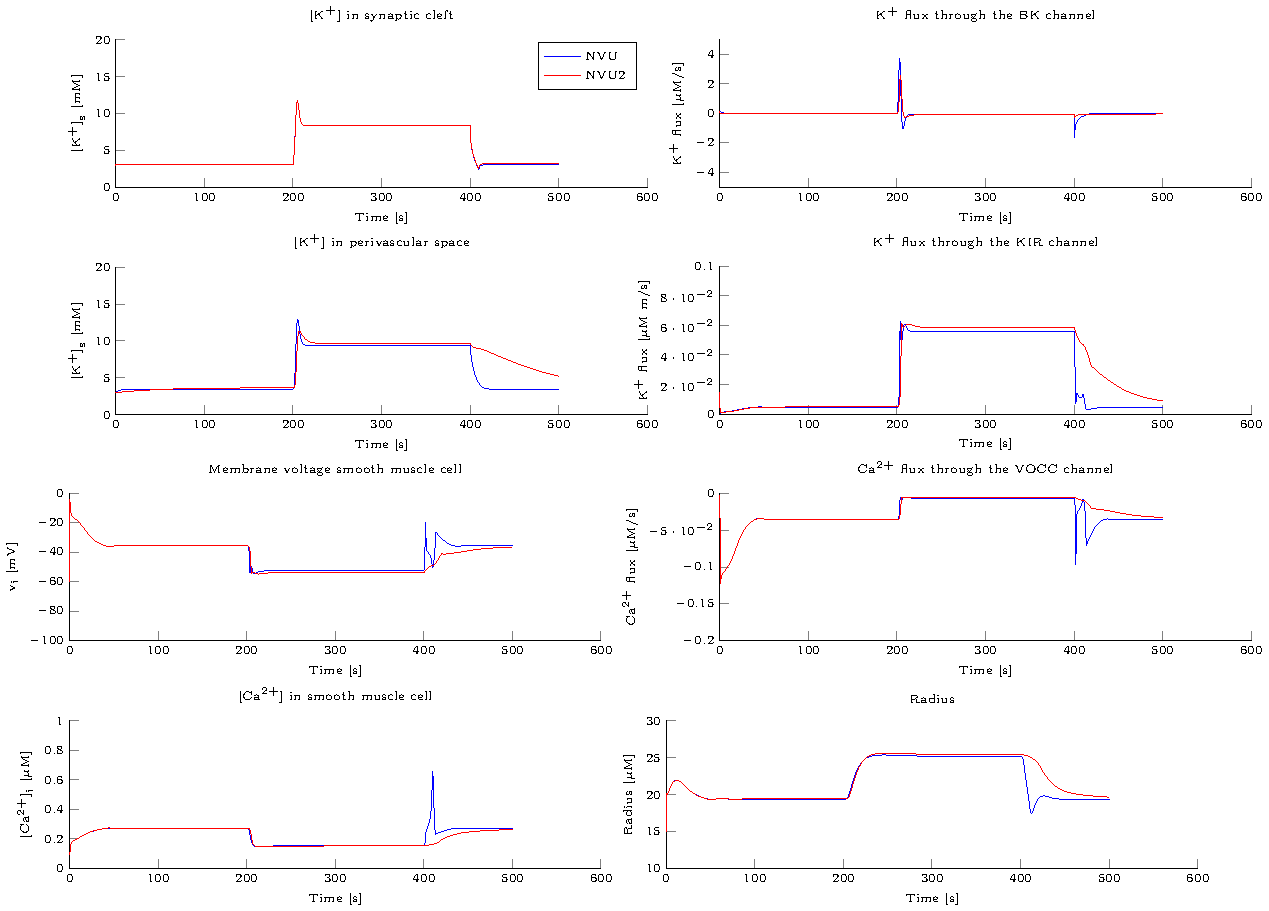
\includegraphics{figures/fig6_NVU_12.pdf}
		\caption{Overview 2, differences between NVU 1.1  \& 1.0  }
		\label{fig:NVU10b}
	\end{figure}
		\begin{figure}[h!]
			\centering
			\tiny  
			\setlength\figureheight{2.5 cm} 
			\setlength\figurewidth{9 cm}
			%% % This file was created by matlab2tikz v0.3.3.
% Copyright (c) 2008--2013, Nico Schlömer <nico.schloemer@gmail.com>
% All rights reserved.
% 
% The latest updates can be retrieved from
%   http://www.mathworks.com/matlabcentral/fileexchange/22022-matlab2tikz
% where you can also make suggestions and rate matlab2tikz.
% 
% 
% 
\tiny 
\newlength\figureheight 
\newlength\figurewidth 
\setlength\figureheight{2.5 cm} 
\setlength\figurewidth{9 cm}
\begin{tikzpicture}

\begin{axis}[%
width=\figurewidth,
height=\figureheight,
scale only axis,
xmin=0,
xmax=600,
xlabel={Time [s]},
ymin=-5,
ymax=5,
ylabel={$\text{K}^\text{+}\text{ flux [}\mu\text{M/s]}$},
name=plot3,
title={$\text{K}^\text{+}\text{ flux through the BK channel}$},
axis x line*=bottom,
axis y line*=left
]
\addplot [
color=blue,
solid,
forget plot
]
table[row sep=crcr]{
0 0.113285245901639\\
0.00089136 0.112878203971859\\
0.0017827 0.113112280874371\\
0.0026741 0.113282825798199\\
0.0061751 0.113902463021875\\
0.0096762 0.114481322357417\\
0.013177 0.115027385130038\\
0.016678 0.115537371683448\\
0.026472 0.116801403669875\\
0.036266 0.117857142857143\\
0.04606 0.118739034188735\\
0.055854 0.119471682025383\\
0.065648 0.120078049420368\\
0.075699 0.120582737587722\\
0.079199 0.120735226601954\\
0.0827 0.120876237948449\\
0.086201 0.12100378756825\\
0.089702 0.121121841643575\\
0.093202 0.121228418239355\\
0.10095 0.121431382193802\\
0.1087 0.121590070666164\\
0.11645 0.121707764952781\\
0.12421 0.12179138247639\\
0.14151 0.121856248155556\\
0.15881 0.121785035084268\\
0.17612 0.121605980621998\\
0.19342 0.121336415351071\\
0.21073 0.120994737791184\\
0.2497 0.120026555635696\\
0.28868 0.118878161522448\\
0.32765 0.117626618587117\\
0.36662 0.116319472899218\\
0.37628 0.115991673905561\\
0.38594 0.115660340249779\\
0.39561 0.11532737851348\\
0.40527 0.114994673440957\\
0.41493 0.114660089156942\\
0.43002 0.114137043774686\\
0.44221 0.113712347176243\\
0.4544 0.113289521124914\\
0.46659 0.11286484537603\\
0.47879 0.112440183546378\\
0.49098 0.112017371353655\\
0.51139 0.111305758578873\\
0.52695 0.110766608764052\\
0.54251 0.110227291349163\\
0.55807 0.109689630309386\\
0.57363 0.109153625563294\\
0.58919 0.108619277029463\\
0.6088 0.107948940632835\\
0.6284 0.107283661330231\\
0.64801 0.106618273579341\\
0.66761 0.105957823329892\\
0.68722 0.105300671800754\\
0.73766 0.103629243675449\\
0.78811 0.101982501556509\\
0.83855 0.100362081394587\\
0.889 0.0987679806022478\\
0.93944 0.0972017890201347\\
1.0031 0.0952638390589931\\
1.0667 0.0933669708238455\\
1.1303 0.0915111802768449\\
1.1939 0.0896964633806739\\
1.2576 0.0879226182675927\\
1.3769 0.0846996773189628\\
1.4783 0.0820647634022898\\
1.5797 0.0795217426910163\\
1.6811 0.0770669549266247\\
1.7825 0.0746961905073864\\
1.8839 0.0724070161646932\\
2.0684 0.0684402738200518\\
2.2528 0.06471243285733\\
2.4373 0.061205908361445\\
2.6218 0.0579068891545352\\
2.8063 0.0547970328644648\\
2.9907 0.0518683477976093\\
3.3424 0.046736638721509\\
3.694 0.0421380970314214\\
4.0456 0.0380079903068409\\
4.3972 0.034290626279165\\
4.7489 0.0309417774575938\\
5.2238 0.0269336564280568\\
5.6986 0.0234376279123074\\
6.1735 0.020384105309691\\
6.6484 0.0177104310951749\\
7.1233 0.0153688725891483\\
7.8241 0.0124291889059891\\
8.525 0.0100004911752186\\
9.2258 0.00798896493008939\\
9.9266 0.00631962408723272\\
10.627 0.00493139919447264\\
11.627 0.00334359343789908\\
12.627 0.00211319951537378\\
13.627 0.00115228069026491\\
14.627 0.000395674383575101\\
15.627 -0.000206260846786077\\
16.627 -0.000691394610170601\\
17.627 -0.00108886996954714\\
18.627 -0.00142226333540718\\
19.627 -0.00170699760961394\\
20.627 -0.00195471364484757\\
21.627 -0.00217459641769541\\
22.627 -0.00237254003078031\\
23.627 -0.00255361996136088\\
24.627 -0.00272160188611284\\
25.627 -0.00287910540620191\\
26.627 -0.00302711287206523\\
27.627 -0.00316677035921281\\
28.627 -0.00329889649300894\\
29.627 -0.00342414617374505\\
30.627 -0.00354268312649399\\
31.627 -0.0036551622515472\\
32.627 -0.00376158354890468\\
33.627 -0.00386227446871214\\
34.627 -0.00395788991126101\\
35.627 -0.0040484298765513\\
36.627 -0.00413422181472871\\
37.627 -0.00421559317593896\\
38.627 -0.00429270768525492\\
39.627 -0.00436556534267658\\
40.627 -0.00443432987327679\\
41.627 -0.00449818265169128\\
42.627 -0.00455663250270146\\
43.627 -0.0046086970758702\\
44.627 -0.00465323029568748\\
45.627 -0.00468908608664331\\
46.627 -0.00471528209830053\\
47.627 -0.0047316546055863\\
48.627 -0.00473836733357346\\
49.627 -0.00473689380791774\\
50.627 -0.00472870755427486\\
51.627 -0.00471610072366482\\
52.627 -0.00470103801696192\\
53.627 -0.00468532040996758\\
54.627 -0.00467058515341039\\
55.627 -0.00465765087265464\\
56.627 -0.00464717246799175\\
57.627 -0.00463931366449458\\
58.627 -0.00463407446216314\\
59.627 -0.00463129113592456\\
60.627 -0.00463063623563312\\
61.627 -0.00463178231114313\\
62.627 -0.00463440191230885\\
63.627 -0.00463816758898458\\
64.627 -0.00464275189102459\\
65.627 -0.00464782736828318\\
66.627 -0.00465306657061462\\
67.627 -0.00465830577294607\\
68.627 -0.00466338125020466\\
69.627 -0.00466780182717181\\
70.627 -0.00467189495399325\\
71.627 -0.00467516945545041\\
72.627 -0.00467778905661613\\
73.627 -0.00467959003241756\\
74.627 -0.00468073610792757\\
75.627 -0.004681391008219\\
76.627 -0.00468122728314614\\
77.627 -0.00468089983300043\\
78.627 -0.00468008120763614\\
79.627 -0.00467893513212613\\
80.627 -0.00467778905661613\\
81.627 -0.00467664298110613\\
82.627 -0.00467533318052327\\
83.627 -0.00467435083008612\\
84.627 -0.00467336847964897\\
85.627 -0.00467254985428469\\
86.627 -0.00467205867906611\\
87.627 -0.0046717312289204\\
88.627 -0.00467156750384754\\
89.627 -0.00467140377877468\\
90.627 -0.00467156750384754\\
91.627 -0.00467189495399325\\
92.627 -0.00467222240413897\\
93.627 -0.00467254985428469\\
94.627 -0.00467304102950326\\
95.627 -0.00467336847964897\\
96.627 -0.00467369592979469\\
97.627 -0.00467418710501326\\
98.627 -0.00467435083008612\\
99.627 -0.00467467828023184\\
100.63 -0.00467484200530469\\
101.63 -0.00467500573037755\\
102.63 -0.00467516945545041\\
103.63 -0.00467516945545041\\
104.63 -0.00467516945545041\\
105.63 -0.00467516945545041\\
106.63 -0.00467516945545041\\
107.63 -0.00467500573037755\\
108.63 -0.00467500573037755\\
109.63 -0.00467500573037755\\
110.63 -0.00467484200530469\\
111.63 -0.00467484200530469\\
112.63 -0.00467467828023184\\
113.63 -0.00467467828023184\\
114.63 -0.00467467828023184\\
115.63 -0.00467451455515898\\
116.63 -0.00467451455515898\\
117.63 -0.00467451455515898\\
118.63 -0.00467451455515898\\
119.63 -0.00467451455515898\\
120.63 -0.00467451455515898\\
121.63 -0.00467451455515898\\
122.63 -0.00467451455515898\\
123.63 -0.00467451455515898\\
124.63 -0.00467467828023184\\
125.63 -0.00467467828023184\\
126.63 -0.00467467828023184\\
127.63 -0.00467467828023184\\
128.63 -0.00467467828023184\\
129.63 -0.00467467828023184\\
130.63 -0.00467467828023184\\
131.63 -0.00467467828023184\\
132.63 -0.00467467828023184\\
133.63 -0.00467467828023184\\
134.63 -0.00467467828023184\\
135.63 -0.00467467828023184\\
136.63 -0.00467467828023184\\
137.63 -0.00467467828023184\\
138.63 -0.00467467828023184\\
139.63 -0.00467467828023184\\
140.63 -0.00467467828023184\\
141.63 -0.00467467828023184\\
142.63 -0.00467467828023184\\
143.63 -0.00467467828023184\\
144.63 -0.00467467828023184\\
145.63 -0.00467467828023184\\
146.63 -0.00467467828023184\\
147.63 -0.00467467828023184\\
148.63 -0.00467467828023184\\
149.63 -0.00467467828023184\\
150.63 -0.00467467828023184\\
151.63 -0.00467467828023184\\
152.63 -0.00467467828023184\\
153.63 -0.00467467828023184\\
154.63 -0.00467467828023184\\
155.63 -0.00467467828023184\\
156.63 -0.00467467828023184\\
157.63 -0.00467467828023184\\
158.63 -0.00467467828023184\\
159.63 -0.00467467828023184\\
160.63 -0.00467467828023184\\
161.63 -0.00467467828023184\\
162.63 -0.00467467828023184\\
163.63 -0.00467467828023184\\
164.63 -0.00467467828023184\\
165.63 -0.00467467828023184\\
166.63 -0.00467467828023184\\
167.63 -0.00467467828023184\\
168.63 -0.00467467828023184\\
169.63 -0.00467467828023184\\
170.63 -0.00467467828023184\\
171.63 -0.00467467828023184\\
172.63 -0.00467467828023184\\
173.63 -0.00467467828023184\\
174.63 -0.00467467828023184\\
175.63 -0.00467467828023184\\
176.63 -0.00467467828023184\\
177.63 -0.00467467828023184\\
178.63 -0.00467467828023184\\
179.63 -0.00467467828023184\\
180.63 -0.00467467828023184\\
181.63 -0.00467467828023184\\
182.63 -0.00467467828023184\\
183.63 -0.00467467828023184\\
184.63 -0.00467467828023184\\
185.63 -0.00467467828023184\\
186.63 -0.00467467828023184\\
187.63 -0.00467467828023184\\
188.63 -0.00467467828023184\\
189.63 -0.00467467828023184\\
190.63 -0.00467467828023184\\
191.63 -0.00467467828023184\\
192.63 -0.00467467828023184\\
193.63 -0.00467467828023184\\
194.63 -0.00467467828023184\\
195.63 -0.00467467828023184\\
196.63 -0.00467467828023184\\
197.19 -0.00467467828023184\\
197.62 -0.00467467828023184\\
197.92 -0.00467467828023184\\
198.17 -0.00467467828023184\\
198.37 -0.00467467828023184\\
198.57 -0.00467467828023184\\
198.71 -0.00467467828023184\\
198.85 -0.00467467828023184\\
198.97 -0.00467467828023184\\
199.09 -0.00467467828023184\\
199.21 -0.00467467828023184\\
199.4 -0.00467467828023184\\
199.6 -0.00467467828023184\\
199.8 -0.00467467828023184\\
199.99 -0.00467467828023184\\
200.31 0.0404227191121267\\
200.54 0.132578861788618\\
200.77 0.287879033171979\\
201.01 0.510997244646396\\
201.24 0.804941399047634\\
201.54 1.28985968879899\\
201.84 1.88951097614981\\
202.14 2.54914892280636\\
202.43 3.15179100289927\\
202.73 3.57300902071825\\
203.03 3.73064635045466\\
203.33 3.59564441597658\\
203.42 3.5004337305392\\
203.51 3.38213407040671\\
203.6 3.24436967657846\\
203.69 3.09077984149071\\
203.78 2.92416374833957\\
203.89 2.69758337724912\\
204 2.45922076361561\\
204.12 2.21343162815787\\
204.23 1.96367441512819\\
204.34 1.71384679632502\\
204.53 1.31970514363844\\
204.71 0.94264978153003\\
204.89 0.590486314111082\\
205.08 0.268674290928894\\
205.45 -0.285093367675467\\
205.83 -0.682111394248271\\
206.2 -0.925025373350732\\
206.58 -1.03613221994279\\
207.23 -1.00983479273606\\
207.87 -0.851895378000717\\
208.52 -0.666628530568466\\
209.17 -0.501485247493645\\
209.82 -0.374605847018705\\
210.52 -0.272003992300563\\
211.23 -0.195921101388137\\
211.93 -0.144870132645647\\
212.64 -0.114620874346519\\
213.34 -0.096010539809144\\
214.34 -0.0791862485402603\\
215.34 -0.068588191734784\\
216.34 -0.0626030615877537\\
217.34 -0.0596146726283713\\
218.34 -0.0580332350805246\\
219.34 -0.0570521309467869\\
220.34 -0.0565230392436065\\
221.34 -0.0561955345446261\\
222.34 -0.0560146949934499\\
223.34 -0.0559150196502819\\
224.34 -0.055856638377855\\
225.34 -0.0558224639744831\\
226.34 -0.055806800706271\\
227.34 -0.0557996810389019\\
228.34 -0.0557954092384804\\
229.34 -0.0557911374380589\\
230.34 -0.0557854417041636\\
231.34 -0.0557825938372159\\
232.34 -0.0557811699037421\\
233.34 -0.0557783220367944\\
234.34 -0.0557754741698468\\
235.34 -0.0557712023694253\\
236.34 -0.0557683545024776\\
237.34 -0.05576550663553\\
238.34 -0.0557640827020562\\
239.34 -0.0557612348351085\\
240.34 -0.0557598109016347\\
241.34 -0.055756963034687\\
242.34 -0.0557541151677394\\
243.34 -0.0557526912342655\\
244.34 -0.0557512673007917\\
245.34 -0.0557498433673179\\
246.34 -0.0557484194338441\\
247.34 -0.0557469955003702\\
248.34 -0.0557455715668964\\
249.34 -0.0557441476334226\\
250.34 -0.0557427236999487\\
251.34 -0.0557412997664749\\
252.34 -0.0557398758330011\\
253.34 -0.0557398758330011\\
254.34 -0.0557384518995273\\
255.34 -0.0557370279660534\\
256.34 -0.0557356040325796\\
257.34 -0.0557341800991058\\
258.34 -0.0557341800991058\\
259.34 -0.0557327561656319\\
260.34 -0.0557313322321581\\
261.34 -0.0557299082986843\\
262.34 -0.0557284843652105\\
263.34 -0.0557284843652105\\
264.34 -0.0557270604317366\\
265.34 -0.0557256364982628\\
266.34 -0.055724212564789\\
267.34 -0.055724212564789\\
268.34 -0.0557227886313151\\
269.34 -0.0557213646978413\\
270.34 -0.0557213646978413\\
271.34 -0.0557199407643675\\
272.34 -0.0557185168308937\\
273.34 -0.0557185168308937\\
274.34 -0.0557170928974198\\
275.34 -0.0557170928974198\\
276.34 -0.055715668963946\\
277.34 -0.055715668963946\\
278.34 -0.0557142450304722\\
279.34 -0.0557142450304722\\
280.34 -0.0557128210969984\\
281.34 -0.0557128210969984\\
282.34 -0.0557113971635245\\
283.34 -0.0557113971635245\\
284.34 -0.0557099732300507\\
285.34 -0.0557099732300507\\
286.34 -0.0557085492965769\\
287.34 -0.0557085492965769\\
288.34 -0.0557085492965769\\
289.34 -0.055707125363103\\
290.34 -0.055707125363103\\
291.34 -0.0557057014296292\\
292.34 -0.0557057014296292\\
293.34 -0.0557057014296292\\
294.34 -0.0557042774961554\\
295.34 -0.0557042774961554\\
296.34 -0.0557042774961554\\
297.34 -0.0557028535626816\\
298.34 -0.0557028535626816\\
299.34 -0.0557028535626816\\
300.34 -0.0557014296292077\\
301.34 -0.0557014296292077\\
302.34 -0.0557014296292077\\
303.34 -0.0557014296292077\\
304.34 -0.0557000056957339\\
305.34 -0.0557000056957339\\
306.34 -0.0557000056957339\\
307.34 -0.0557000056957339\\
308.34 -0.0556985817622601\\
309.34 -0.0556985817622601\\
310.34 -0.0556985817622601\\
311.34 -0.0556985817622601\\
312.34 -0.0556971578287862\\
313.34 -0.0556971578287862\\
314.34 -0.0556971578287862\\
315.34 -0.0556971578287862\\
316.34 -0.0556957338953124\\
317.34 -0.0556957338953124\\
318.34 -0.0556957338953124\\
319.34 -0.0556957338953124\\
320.34 -0.0556957338953124\\
321.34 -0.0556957338953124\\
322.34 -0.0556943099618386\\
323.34 -0.0556943099618386\\
324.34 -0.0556943099618386\\
325.34 -0.0556943099618386\\
326.34 -0.0556943099618386\\
327.34 -0.0556943099618386\\
328.34 -0.0556928860283648\\
329.34 -0.0556928860283648\\
330.34 -0.0556928860283648\\
331.34 -0.0556928860283648\\
332.34 -0.0556928860283648\\
333.34 -0.0556928860283648\\
334.34 -0.0556928860283648\\
335.34 -0.0556914620948909\\
336.34 -0.0556914620948909\\
337.34 -0.0556914620948909\\
338.34 -0.0556914620948909\\
339.34 -0.0556914620948909\\
340.34 -0.0556914620948909\\
341.34 -0.0556914620948909\\
342.34 -0.0556914620948909\\
343.34 -0.0556914620948909\\
344.34 -0.0556900381614171\\
345.34 -0.0556900381614171\\
346.34 -0.0556900381614171\\
347.34 -0.0556900381614171\\
348.34 -0.0556900381614171\\
349.34 -0.0556900381614171\\
350.34 -0.0556900381614171\\
351.34 -0.0556900381614171\\
352.34 -0.0556900381614171\\
353.34 -0.0556900381614171\\
354.34 -0.0556900381614171\\
355.34 -0.0556886142279433\\
356.34 -0.0556886142279433\\
357.34 -0.0556886142279433\\
358.34 -0.0556886142279433\\
359.34 -0.0556886142279433\\
360.34 -0.0556886142279433\\
361.34 -0.0556886142279433\\
362.34 -0.0556886142279433\\
363.34 -0.0556886142279433\\
364.34 -0.0556886142279433\\
365.34 -0.0556886142279433\\
366.34 -0.0556886142279433\\
367.34 -0.0556886142279433\\
368.34 -0.0556886142279433\\
369.34 -0.0556886142279433\\
370.34 -0.0556886142279433\\
371.34 -0.0556871902944694\\
372.34 -0.0556871902944694\\
373.34 -0.0556871902944694\\
374.34 -0.0556871902944694\\
375.34 -0.0556871902944694\\
376.34 -0.0556871902944694\\
377.34 -0.0556871902944694\\
378.34 -0.0556871902944694\\
379.34 -0.0556871902944694\\
380.34 -0.0556871902944694\\
381.34 -0.0556871902944694\\
382.34 -0.0556871902944694\\
383.34 -0.0556871902944694\\
384.34 -0.0556871902944694\\
385.34 -0.0556871902944694\\
386.34 -0.0556871902944694\\
387.34 -0.0556871902944694\\
388.34 -0.0556871902944694\\
389.34 -0.0556871902944694\\
390.34 -0.0556871902944694\\
391.34 -0.0556871902944694\\
392.34 -0.0556871902944694\\
393.34 -0.0556871902944694\\
394.34 -0.0556871902944694\\
395.34 -0.0556871902944694\\
396.34 -0.0556871902944694\\
397.34 -0.0556871902944694\\
398.17 -0.0556871902944694\\
398.58 -0.0556871902944694\\
398.9 -0.0556857663609956\\
399.16 -0.0556857663609956\\
399.42 -0.0556857663609956\\
399.62 -0.0556857663609956\\
399.82 -0.0556857663609956\\
399.88 -0.0556857663609956\\
399.94 -0.0556857663609956\\
399.99 -0.0556857663609956\\
400.03 -0.613773265169531\\
400.08 -1.06824946947147\\
400.15 -1.51061404758513\\
400.22 -1.65763968072976\\
400.29 -1.64534759358289\\
400.36 -1.57516265266522\\
400.48 -1.4513595338741\\
400.59 -1.34536436147403\\
400.71 -1.26300652472527\\
400.83 -1.19637332416638\\
401.11 -1.06278722426471\\
401.23 -1.01453734991732\\
401.33 -0.977660386049257\\
401.41 -0.948929610741349\\
401.5 -0.92134556045794\\
401.56 -0.899920640646418\\
401.63 -0.879272254710851\\
401.66 -0.868478072456232\\
401.69 -0.860026587290119\\
401.72 -0.851673050516731\\
401.75 -0.843485678758874\\
401.78 -0.835423265500933\\
401.81 -0.82495080449126\\
401.85 -0.814715631921023\\
401.89 -0.804715218745022\\
401.93 -0.794926402410756\\
401.98 -0.781348757646922\\
402.03 -0.768200873235759\\
402.09 -0.755457501161171\\
402.14 -0.743104875604549\\
402.2 -0.731129196337742\\
402.37 -0.693788684191364\\
402.55 -0.660001751364605\\
402.68 -0.637826697070689\\
402.81 -0.617085132859966\\
402.93 -0.597627496407519\\
403.06 -0.579336172712586\\
403.27 -0.551105155428588\\
403.44 -0.530892617350628\\
403.6 -0.512081509523246\\
403.77 -0.494494746669433\\
403.93 -0.478021325254685\\
404.15 -0.45772833549271\\
404.37 -0.439014919577652\\
404.59 -0.421671409315561\\
404.81 -0.40556615250597\\
405.2 -0.379667924528302\\
405.58 -0.356512241740238\\
405.97 -0.335619988414281\\
406.36 -0.316594923329095\\
406.74 -0.299145693835142\\
407.4 -0.27236756354157\\
408.07 -0.248811534371677\\
408.61 -0.231012508850602\\
409.16 -0.214719848053181\\
409.32 -0.210204211060375\\
409.48 -0.205796871277694\\
409.65 -0.201479478205536\\
409.81 -0.19728476504613\\
409.97 -0.193216822280744\\
410.14 -0.178135644720219\\
410.3 -0.186894020737512\\
410.47 -0.207784075400202\\
410.63 -0.202390143472946\\
410.8 -0.180192372758471\\
410.96 -0.174310150072616\\
411.13 -0.176984858033968\\
411.38 -0.171686259270054\\
411.64 -0.153124087591241\\
411.89 -0.141657325730624\\
412.14 -0.136666178695164\\
412.4 -0.128909659349964\\
412.65 -0.119126707305147\\
413.05 -0.106349335857185\\
413.31 -0.100801724278693\\
413.53 -0.0950912328274826\\
413.72 -0.0899944440813125\\
413.89 -0.0860477280156914\\
414.02 -0.0831973712174467\\
414.15 -0.0804182540590919\\
414.28 -0.0777183600713013\\
414.41 -0.0751099916586251\\
414.63 -0.0710448396014985\\
414.85 -0.067222958490813\\
415.07 -0.0636278841433481\\
415.47 -0.0574211077648291\\
415.87 -0.051843302884458\\
416.28 -0.046856478601133\\
416.68 -0.0424024102698454\\
417.45 -0.0351608941292066\\
418.22 -0.0292985702821768\\
418.99 -0.0245389629532576\\
419.75 -0.0206708485513537\\
420.75 -0.0166814072327044\\
421.75 -0.0136381354821803\\
422.75 -0.0113253406708595\\
423.75 -0.00957448899371069\\
424.75 -0.00825520833333333\\
425.75 -0.0072667714884696\\
426.75 -0.0065310534591195\\
427.75 -0.00599269523060797\\
428.75 -0.0056028891509434\\
429.75 -0.00532199947589099\\
430.75 -0.00512169156184486\\
431.75 -0.00498116483228512\\
432.75 -0.00488485980083857\\
433.75 -0.00482016509433962\\
434.75 -0.00477807258909853\\
435.75 -0.00475088443396226\\
436.75 -0.00473319575471698\\
437.75 -0.00472140330188679\\
438.75 -0.00471239517819707\\
439.75 -0.00470469732704403\\
440.75 -0.00469732704402516\\
441.75 -0.00468995676100629\\
442.75 -0.00468258647798742\\
443.75 -0.00467505241090147\\
444.75 -0.0046676821278826\\
445.75 -0.0046606394129979\\
446.75 -0.00465441561844864\\
447.75 -0.00464868317610063\\
448.75 -0.00464393343815514\\
449.75 -0.00464000262054507\\
450.75 -0.00463689072327044\\
451.75 -0.00463459774633124\\
452.75 -0.00463312368972746\\
453.75 -0.00463214098532495\\
454.75 -0.00463164963312369\\
455.75 -0.00463164963312369\\
456.75 -0.00463197720125786\\
457.75 -0.00463263233752621\\
458.75 -0.00463328747379455\\
459.75 -0.00463410639412998\\
460.75 -0.00463508909853249\\
461.75 -0.00463590801886792\\
462.75 -0.00463656315513627\\
463.75 -0.00463721829140461\\
464.75 -0.00463787342767296\\
465.75 -0.00463820099580713\\
466.75 -0.0046385285639413\\
467.75 -0.00463869234800838\\
468.75 -0.00463885613207547\\
469.75 -0.00463885613207547\\
470.75 -0.00463869234800838\\
471.75 -0.0046385285639413\\
472.75 -0.00463836477987421\\
473.75 -0.00463820099580713\\
474.75 -0.00463787342767296\\
475.75 -0.00463770964360587\\
476.75 -0.00463754585953878\\
477.75 -0.0046373820754717\\
478.75 -0.00463721829140461\\
479.75 -0.00463705450733753\\
480.75 -0.00463705450733753\\
481.75 -0.00463689072327044\\
482.75 -0.00463689072327044\\
483.75 -0.00463689072327044\\
484.75 -0.00463689072327044\\
485.75 -0.00463689072327044\\
486.75 -0.00463689072327044\\
487.75 -0.00463705450733753\\
488.75 -0.00463705450733753\\
489.75 -0.00463705450733753\\
490.75 -0.00463721829140461\\
491.75 -0.00463721829140461\\
492.75 -0.00463721829140461\\
493.75 -0.00463721829140461\\
494.75 -0.00463721829140461\\
495.75 -0.0046373820754717\\
496.75 -0.0046373820754717\\
497.75 -0.0046373820754717\\
498.75 -0.0046373820754717\\
499.75 -0.0046373820754717\\
500 -0.0046373820754717\\
};
\addplot [
color=red,
solid,
forget plot
]
table[row sep=crcr]{
0 0.113285245901639\\
0.0011996 0.110367673587195\\
0.0023992 0.108143520112822\\
0.0035988 0.105901838277496\\
0.0085566 0.0970384703683054\\
0.013514 0.0889000032796563\\
0.018472 0.0814650224656456\\
0.02343 0.0746847482085171\\
0.033542 0.0627180899908173\\
0.043655 0.0529080921538083\\
0.053767 0.0448848077396081\\
0.063879 0.0383366674318696\\
0.073991 0.033011953367111\\
0.084819 0.0284187053190792\\
0.095647 0.0247548778488277\\
0.10647 0.0218376481776\\
0.1173 0.0195156741867786\\
0.12813 0.0176692407325431\\
0.14659 0.0153720796786622\\
0.16505 0.0138232015214112\\
0.18351 0.0127727138594708\\
0.20197 0.0120608196721311\\
0.22042 0.0115807937574794\\
0.26398 0.0110246701090075\\
0.30753 0.0107948137949121\\
0.35108 0.0106624926244018\\
0.37397 0.0106097061282022\\
0.38969 0.0105893729308028\\
0.4054 0.0105762517413751\\
0.42111 0.0105659171364888\\
0.43393 0.01055787731288\\
0.44676 0.0105503294109935\\
0.45959 0.0105434372900244\\
0.47242 0.0105372097215621\\
0.48525 0.0105309734513274\\
0.50035 0.0105240818734534\\
0.51544 0.0105173543967749\\
0.53054 0.0105107910132245\\
0.54564 0.0105045638529735\\
0.56073 0.0104980007865758\\
0.57728 0.0104911102007374\\
0.59382 0.0104840559761413\\
0.61036 0.010477001982729\\
0.6269 0.0104701197830469\\
0.64344 0.0104632299927902\\
0.65998 0.0104561765717937\\
0.69992 0.0104391211023906\\
0.73986 0.0104222375147464\\
0.77979 0.0104050201527018\\
0.81973 0.0103881379536332\\
0.85967 0.0103709225551715\\
0.99616 0.010313068265592\\
1.1327 0.0102558768121877\\
1.2692 0.0101998427466911\\
1.4056 0.0101449607705034\\
1.6062 0.0100669887806076\\
1.8067 0.00999181106488912\\
2.0072 0.00991942483745762\\
2.2078 0.00984949969703421\\
2.4083 0.00978187177597642\\
2.8551 0.00963745926738607\\
3.302 0.00950090877830721\\
3.7488 0.00936993434087076\\
4.1956 0.00924338927548097\\
4.6425 0.00912044010740717\\
5.3586 0.00892969415154889\\
6.0748 0.00874437185847373\\
6.791 0.00856361641861912\\
7.5072 0.00838648940698779\\
8.2234 0.00821277710468581\\
9.2234 0.00797521202396935\\
10.223 0.00774255869543862\\
11.223 0.00751432594387504\\
12.223 0.00728904024362291\\
12.523 0.00722158551360555\\
12.823 0.00715363960836963\\
13.123 0.00708487507776941\\
13.423 0.00701267232063918\\
13.513 0.00698975081043911\\
13.603 0.00696568322472904\\
13.693 0.00693965093814467\\
13.783 0.00691001669995743\\
13.873 0.00687366973378303\\
13.929 0.00684812862241724\\
13.948 0.00684059726906578\\
13.967 0.00683683159239006\\
13.986 0.00683945119355578\\
14.004 0.00684894724778153\\
14.023 0.00686581093028586\\
14.079 0.00695864304659616\\
14.134 0.00710239366056518\\
14.189 0.00722338648940699\\
14.244 0.00711516421624808\\
14.299 0.00654998526474344\\
14.354 0.00579865090539965\\
14.409 0.00552932316054881\\
14.465 0.00608435115753627\\
14.52 0.00732325878385016\\
14.575 0.00895510658502243\\
14.631 0.0107907921019025\\
14.686 0.0127111234814499\\
14.742 0.0145787353875372\\
14.811 0.0166213693965094\\
14.88 0.0181440125740856\\
14.95 0.0190674219850028\\
15.019 0.0194308916467468\\
15.089 0.0193342938537608\\
15.202 0.0184861979763581\\
15.315 0.0171403778774682\\
15.428 0.0156142964733619\\
15.541 0.0141058973771243\\
15.654 0.0127194734601657\\
15.804 0.0111493500114608\\
15.954 0.00995955990700416\\
16.104 0.00918317561151315\\
16.255 0.00882494515210059\\
16.405 0.00882314417629916\\
16.675 0.00914437276924588\\
16.946 0.00911981400831723\\
17.216 0.00845148826091228\\
17.487 0.00769606077474705\\
17.757 0.00710190248534661\\
18.061 0.00657929205278496\\
18.364 0.00616916074527653\\
18.667 0.00586233995874128\\
18.971 0.00563410720717771\\
19.274 0.00545581060283572\\
19.375 0.00540636563083271\\
19.476 0.00536690788827401\\
19.576 0.00533743737515963\\
19.677 0.00531533449032385\\
19.778 0.00529699728216379\\
19.938 0.00526900029470513\\
20.097 0.00524149448246504\\
20.257 0.0052126788696421\\
20.416 0.005182880906382\\
20.576 0.00515341039326762\\
20.994 0.0050780968597531\\
21.411 0.00500016372507286\\
21.828 0.00491977471429975\\
22.056 0.00487491404433675\\
22.119 0.00486361701430957\\
22.183 0.0048546121353024\\
22.247 0.00484953665804381\\
22.31 0.00484740823209666\\
22.432 0.00484822685746095\\
22.554 0.00485199253413668\\
22.676 0.00485919643734241\\
22.798 0.00487032974229674\\
22.92 0.00488424637348964\\
23.367 0.00494744425161269\\
23.684 0.00500278332623858\\
24 0.00505959592652019\\
24.242 0.00509921739415174\\
24.484 0.00513048888306755\\
24.726 0.00514948099151904\\
24.968 0.00515308294312191\\
25.298 0.00513048888306755\\
25.628 0.00507564098366024\\
25.958 0.00499165002128426\\
26.288 0.00488539244899964\\
26.618 0.0047648907953764\\
27.087 0.00458364713972298\\
27.556 0.0044056779855267\\
28.025 0.00424064311208619\\
28.494 0.00409279937129572\\
28.964 0.00396198303808245\\
29.615 0.00380578931857625\\
30.266 0.00367431808507155\\
30.917 0.00356167523494548\\
31.569 0.00346180294050231\\
32.372 0.00334752283964766\\
33.175 0.0032329152886473\\
33.979 0.00310913913356691\\
34.782 0.00297226497265791\\
35.586 0.00282458495694031\\
36.23 0.00270228232751564\\
36.875 0.00258030714823668\\
37.52 0.00246078784505059\\
38.164 0.00234487049346737\\
38.969 0.00220603163168408\\
39.774 0.0020729231474508\\
40.579 0.00194439896525754\\
41.384 0.00181865810930286\\
42.189 0.0016943907790039\\
43.189 0.00154114411080913\\
44.189 0.00138912538066079\\
45.189 0.00123933331150332\\
46.189 0.00109296309636858\\
47.189 0.000950882478142703\\
48.189 0.000813386161956842\\
49.189 0.000680294050230852\\
50.189 0.000551164085268018\\
51.189 0.000425717934444481\\
52.189 0.000303742755165526\\
53.189 0.000185074822358296\\
54.189 6.95798814630473e-05\\
55.189 -4.2900880840892e-05\\
56.189 -0.000152554111136579\\
57.189 -0.00025956973050853\\
58.189 -0.00036412456203543\\
59.189 -0.000466354497527751\\
60.189 -0.000566325027014637\\
61.189 -0.000664118013032516\\
62.189 -0.000759782573103245\\
63.189 -0.000853351452241396\\
64.189 -0.000944890140476113\\
65.189 -0.00103444775532925\\
66.189 -0.00112212253184453\\
67.189 -0.00120791447002194\\
68.189 -0.00129185631487606\\
69.189 -0.00137348963620289\\
70.189 -0.00145324011919185\\
71.189 -0.0015311732538721\\
72.189 -0.00160764923540391\\
73.189 -0.00168243884868529\\
74.189 -0.00175562395625266\\
75.189 -0.00182717181309146\\
76.189 -0.0018965912439831\\
77.189 -0.00196437342414617\\
78.189 -0.00203051835358067\\
79.189 -0.00209518975735944\\
80.189 -0.0021583876354825\\
81.189 -0.00221994826287698\\
82.189 -0.00228052653983431\\
83.189 -0.00233979501620878\\
84.189 -0.00239791741707325\\
85.189 -0.002454566292282\\
86.189 -0.00250957791676217\\
87.189 -0.00256344346573234\\
88.189 -0.00261616293919251\\
89.189 -0.00266757261206981\\
90.189 -0.00271783620943711\\
91.189 -0.00276711745636727\\
92.189 -0.00281525262778742\\
93.189 -0.00286240544877042\\
94.189 -0.00290857591931628\\
95.189 -0.00295360031435214\\
96.189 -0.00299780608402371\\
97.189 -0.00304086577818527\\
98.189 -0.00308310684698255\\
99.189 -0.00312436556534268\\
100.19 -0.00316480565833852\\
101.19 -0.00320426340089721\\
102.19 -0.00324290251809162\\
103.19 -0.00328072300992174\\
104.19 -0.00331772487638757\\
105.19 -0.00335374439241625\\
106.19 -0.00338927273322637\\
107.19 -0.00342381872359933\\
108.19 -0.00345770981368087\\
109.19 -0.00349078227839811\\
110.19 -0.00352319984282393\\
111.19 -0.00355479878188546\\
112.19 -0.00358590654572841\\
113.19 -0.00361619568420708\\
114.19 -0.00364582992239432\\
115.19 -0.00367480926029012\\
116.19 -0.00370329742296735\\
117.19 -0.00373113068535315\\
118.19 -0.00375830904744753\\
119.19 -0.00378483250925047\\
120.19 -0.00381102852090769\\
121.19 -0.00383640590720063\\
122.19 -0.00386129211827499\\
123.19 -0.00388585087920364\\
124.19 -0.003909591014768\\
125.19 -0.00393300370018665\\
126.19 -0.00395592521038672\\
127.19 -0.00397819182029536\\
128.19 -0.00400013098005829\\
129.19 -0.00402157896460264\\
130.19 -0.00404253577392842\\
131.19 -0.00406316513310848\\
132.19 -0.00408313959199712\\
133.19 -0.00410278660074004\\
134.19 -0.00412210615933724\\
135.19 -0.00414093454271587\\
136.19 -0.00415927175087593\\
137.19 -0.00417744523396313\\
138.19 -0.0041949638167589\\
139.19 -0.00421231867448181\\
140.19 -0.00422918235698615\\
141.19 -0.00424571858934477\\
142.19 -0.00426192737155768\\
143.19 -0.00427780870362487\\
144.19 -0.00429336258554635\\
145.19 -0.00430842529224926\\
146.19 -0.0043233242738793\\
147.19 -0.00433789580536363\\
148.19 -0.00435213988670225\\
149.19 -0.00436605651789515\\
150.19 -0.00437964569894234\\
151.19 -0.00439307115491666\\
152.19 -0.00440616916074528\\
153.19 -0.00441893971642817\\
154.19 -0.00443154654703821\\
155.19 -0.00444366220242968\\
156.19 -0.00445577785782115\\
157.19 -0.00446740233799404\\
158.19 -0.00447902681816693\\
159.19 -0.00449016012312126\\
160.19 -0.00450129342807558\\
161.19 -0.00451193555781132\\
162.19 -0.00452257768754707\\
163.19 -0.0045328923671371\\
164.19 -0.00454304332165428\\
165.19 -0.00455286682602574\\
166.19 -0.0045626903303972\\
167.19 -0.00457202265955008\\
168.19 -0.00458135498870297\\
169.19 -0.004590523592783\\
170.19 -0.00459936474671731\\
171.19 -0.00460804217557877\\
172.19 -0.00461655587936737\\
173.19 -0.00462490585808311\\
174.19 -0.00463309211172599\\
175.19 -0.00464111464029602\\
176.19 -0.00464897344379318\\
177.19 -0.00465666852221749\\
178.19 -0.00466419987556894\\
179.19 -0.00467156750384754\\
180.19 -0.00467877140705328\\
181.19 -0.00468581158518616\\
182.19 -0.00469268803824618\\
183.19 -0.00469940076623334\\
184.19 -0.00470594976914765\\
185.19 -0.00471249877206195\\
186.19 -0.0047188840499034\\
187.19 -0.00472494187759914\\
188.19 -0.00473116343036773\\
189.19 -0.0047370575329906\\
190.19 -0.00474278791054062\\
191.19 -0.00474851828809064\\
192.19 -0.0047540849405678\\
193.19 -0.00475965159304496\\
194.19 -0.0047648907953764\\
195.19 -0.00477029372278071\\
196.19 -0.00477602410033072\\
196.81 -0.00478093585251645\\
197.25 -0.00478601132977504\\
197.57 -0.0047915779822522\\
197.82 -0.00479779953502079\\
198.03 -0.00480483971315367\\
198.24 -0.00481499066767085\\
198.38 -0.0048236680965323\\
198.52 -0.00483512885163234\\
198.63 -0.00484593470644094\\
198.74 -0.00485952388748813\\
198.83 -0.00487245816824388\\
198.92 -0.0048878483250925\\
199.01 -0.0049060218081797\\
199.17 -0.00494220504928125\\
199.32 -0.00498870296997282\\
199.47 -0.00504813517142015\\
199.62 -0.00512312125478896\\
199.84 -0.00526179639149939\\
200.07 -0.00680932452756163\\
200.29 -0.003698143348493\\
200.51 0.00568713758994266\\
200.69 0.018395829285668\\
200.87 0.0352024268633114\\
201.05 0.0587831427974209\\
201.23 0.0939399279134962\\
201.42 0.14471660177443\\
201.6 0.215844259038538\\
201.79 0.312196357076166\\
201.97 0.441597731032853\\
202.15 0.610281429423023\\
202.34 0.819059220389805\\
202.63 1.21478414588761\\
202.92 1.65257825611653\\
203.21 2.0669092688297\\
203.5 2.38853116267768\\
203.79 2.56683765841883\\
204.09 2.58237145855194\\
204.39 2.44330879942787\\
204.69 2.18933333333333\\
204.94 1.92851769356718\\
205.19 1.63679370023213\\
205.44 1.33306986343477\\
205.68 1.04105032822757\\
205.85 0.855362757656923\\
206.02 0.685020266441968\\
206.19 0.531395011600928\\
206.36 0.395051898605904\\
206.6 0.230467000823354\\
206.84 0.0982050949353402\\
207.08 -0.00535614052762626\\
207.32 -0.0845567946654403\\
207.65 -0.162085389647653\\
207.99 -0.211773470294122\\
208.32 -0.241800228963938\\
208.65 -0.25816367379618\\
208.99 -0.265272301274359\\
209.66 -0.263286334056399\\
210.18 -0.254735280693747\\
210.7 -0.244104815944798\\
211.22 -0.232911464568725\\
211.74 -0.22182958107723\\
212.26 -0.210949965808069\\
212.9 -0.19754141560902\\
213.54 -0.184190286284005\\
214.18 -0.171273944313893\\
214.82 -0.159104503118858\\
215.46 -0.147949302193107\\
216.16 -0.137009769018256\\
216.87 -0.127533714025319\\
217.57 -0.11935378218273\\
218.27 -0.112146844383686\\
218.98 -0.105597721609114\\
219.98 -0.0973470986116056\\
220.98 -0.0901488074047704\\
221.98 -0.0841139195443218\\
222.98 -0.0794788180847277\\
223.98 -0.0760085439658241\\
224.98 -0.0731947312210751\\
225.98 -0.0708209327162691\\
226.98 -0.0686322534709861\\
227.98 -0.066752580989676\\
228.98 -0.0651776432894269\\
229.98 -0.0639729441082236\\
230.98 -0.0630672837308651\\
231.98 -0.0623367746529014\\
232.98 -0.0616988252046992\\
233.98 -0.0610964756140975\\
234.98 -0.0605710217159131\\
235.98 -0.0602321110715557\\
236.98 -0.0598049127803489\\
237.98 -0.0596682093271627\\
238.98 -0.0594802420790317\\
239.98 -0.0593179067283731\\
240.98 -0.0591584193663225\\
241.98 -0.0590530437878249\\
242.98 -0.058939124243503\\
243.98 -0.0588593805624778\\
244.98 -0.0587796368814525\\
245.98 -0.0587255250978996\\
246.98 -0.0586728373086508\\
247.98 -0.0586372374510502\\
248.98 -0.0586016375934496\\
249.98 -0.0585774296902812\\
250.98 -0.0585546457814169\\
251.98 -0.0585375578497686\\
252.98 -0.0585218939124244\\
253.98 -0.0585105019579922\\
254.98 -0.05849911000356\\
255.98 -0.0584919900320399\\
256.98 -0.0584848700605198\\
257.98 -0.0584791740833037\\
258.98 -0.0584749021003916\\
259.98 -0.0584706301174795\\
260.98 -0.0584677821288715\\
261.98 -0.0584649341402634\\
262.98 -0.0584620861516554\\
263.98 -0.0584606621573514\\
264.98 -0.0584592381630474\\
265.98 -0.0584578141687433\\
266.98 -0.0584563901744393\\
267.98 -0.0584549661801353\\
268.98 -0.0584535421858313\\
269.98 -0.0584535421858313\\
270.98 -0.0584521181915272\\
271.98 -0.0584521181915272\\
272.98 -0.0584506941972232\\
273.98 -0.0584506941972232\\
274.98 -0.0584492702029192\\
275.98 -0.0584492702029192\\
276.98 -0.0584492702029192\\
277.98 -0.0584478462086152\\
278.98 -0.0584478462086152\\
279.98 -0.0584478462086152\\
280.98 -0.0584478462086152\\
281.98 -0.0584464222143112\\
282.98 -0.0584464222143112\\
283.98 -0.0584464222143112\\
284.98 -0.0584464222143112\\
285.98 -0.0584464222143112\\
286.98 -0.0584449982200071\\
287.98 -0.0584449982200071\\
288.98 -0.0584449982200071\\
289.98 -0.0584449982200071\\
290.98 -0.0584449982200071\\
291.98 -0.0584435742257031\\
292.98 -0.0584435742257031\\
293.98 -0.0584435742257031\\
294.98 -0.0584435742257031\\
295.98 -0.0584435742257031\\
296.98 -0.0584435742257031\\
297.98 -0.0584435742257031\\
298.98 -0.0584421502313991\\
299.98 -0.0584421502313991\\
300.98 -0.0584421502313991\\
301.98 -0.0584421502313991\\
302.98 -0.0584421502313991\\
303.98 -0.0584421502313991\\
304.98 -0.0584421502313991\\
305.98 -0.0584407262370951\\
306.98 -0.0584407262370951\\
307.98 -0.0584407262370951\\
308.98 -0.0584407262370951\\
309.98 -0.0584407262370951\\
310.98 -0.0584407262370951\\
311.98 -0.0584407262370951\\
312.98 -0.0584407262370951\\
313.98 -0.0584407262370951\\
314.98 -0.058439302242791\\
315.98 -0.058439302242791\\
316.98 -0.058439302242791\\
317.98 -0.058439302242791\\
318.98 -0.058439302242791\\
319.98 -0.058439302242791\\
320.98 -0.058439302242791\\
321.98 -0.058439302242791\\
322.98 -0.058439302242791\\
323.98 -0.058439302242791\\
324.98 -0.058439302242791\\
325.98 -0.058437878248487\\
326.98 -0.058437878248487\\
327.98 -0.058437878248487\\
328.98 -0.058437878248487\\
329.98 -0.058437878248487\\
330.98 -0.058437878248487\\
331.98 -0.058437878248487\\
332.98 -0.058437878248487\\
333.98 -0.058437878248487\\
334.98 -0.058437878248487\\
335.98 -0.058437878248487\\
336.98 -0.058437878248487\\
337.98 -0.058437878248487\\
338.98 -0.058437878248487\\
339.98 -0.058437878248487\\
340.98 -0.058436454254183\\
341.98 -0.058436454254183\\
342.98 -0.058436454254183\\
343.98 -0.058436454254183\\
344.98 -0.058436454254183\\
345.98 -0.058436454254183\\
346.98 -0.058436454254183\\
347.98 -0.058436454254183\\
348.98 -0.058436454254183\\
349.98 -0.058436454254183\\
350.98 -0.058436454254183\\
351.98 -0.058436454254183\\
352.98 -0.058436454254183\\
353.98 -0.058436454254183\\
354.98 -0.058436454254183\\
355.98 -0.058436454254183\\
356.98 -0.058436454254183\\
357.98 -0.058436454254183\\
358.98 -0.058436454254183\\
359.98 -0.058436454254183\\
360.98 -0.058436454254183\\
361.98 -0.058436454254183\\
362.98 -0.058436454254183\\
363.98 -0.058436454254183\\
364.98 -0.058435030259879\\
365.98 -0.058435030259879\\
366.98 -0.058435030259879\\
367.98 -0.058435030259879\\
368.98 -0.058435030259879\\
369.98 -0.058435030259879\\
370.98 -0.058435030259879\\
371.98 -0.058435030259879\\
372.98 -0.058435030259879\\
373.98 -0.058435030259879\\
374.98 -0.058435030259879\\
375.98 -0.058435030259879\\
376.98 -0.058435030259879\\
377.98 -0.058435030259879\\
378.98 -0.058435030259879\\
379.98 -0.058435030259879\\
380.98 -0.058435030259879\\
381.98 -0.058435030259879\\
382.98 -0.058435030259879\\
383.98 -0.058435030259879\\
384.98 -0.058435030259879\\
385.98 -0.058435030259879\\
386.98 -0.058435030259879\\
387.98 -0.058435030259879\\
388.98 -0.058435030259879\\
389.98 -0.058435030259879\\
390.98 -0.058435030259879\\
391.98 -0.058435030259879\\
392.98 -0.058435030259879\\
393.98 -0.058435030259879\\
394.98 -0.058435030259879\\
395.98 -0.0584336062655749\\
396.98 -0.0584264862940548\\
397.98 -0.0584649341402634\\
398.44 -0.0584706301174795\\
398.8 -0.0584734781060876\\
399.07 -0.0584720541117836\\
399.35 -0.0584008543965824\\
399.55 -0.0584093983624066\\
399.76 -0.0583396226415094\\
399.96 -0.0582840868636525\\
400.26 -0.20925791326407\\
400.34 -0.238461209416395\\
400.43 -0.244664155681105\\
400.52 -0.241287743593404\\
400.61 -0.23681353220184\\
400.92 -0.22496633527204\\
401.24 -0.218547042933502\\
401.56 -0.207533298737243\\
401.87 -0.192495732924466\\
402.11 -0.1809387056537\\
402.35 -0.170363475048362\\
402.59 -0.160569461462162\\
402.83 -0.151369301890105\\
403.14 -0.140318388086881\\
403.45 -0.13055567841715\\
403.77 -0.122229458695363\\
404.08 -0.114926437806509\\
404.39 -0.108504923903312\\
404.93 -0.0985875706214689\\
405.47 -0.088969253117056\\
406.02 -0.0801084853194375\\
406.56 -0.0745060137457045\\
407.1 -0.0727115476686899\\
408.1 -0.0634064766191548\\
408.77 -0.0573057239587434\\
409.43 -0.0529736416404986\\
410.1 -0.0683297110713372\\
410.61 -0.0805382823170242\\
411.12 -0.0820098134159726\\
411.63 -0.0824234375759146\\
412.15 -0.0855104227547243\\
412.66 -0.0856043973914882\\
413.31 -0.0843292454520285\\
413.95 -0.0840940953995631\\
414.6 -0.0843123501296837\\
415.25 -0.0842178269525768\\
415.9 -0.0841486704862641\\
416.77 -0.084279440335668\\
417.65 -0.0843856641358478\\
418.52 -0.0842964680524485\\
419.4 -0.0839905942291677\\
420.28 -0.0834710473888762\\
421.2 -0.0827558052189817\\
422.12 -0.082009242778059\\
423.04 -0.0813315479203749\\
423.96 -0.0807469340431439\\
424.89 -0.0802390711497951\\
425.81 -0.0797671342489018\\
426.73 -0.0792853993500661\\
427.68 -0.0787628394598037\\
428.64 -0.0782059865767428\\
429.59 -0.0776213726995117\\
430.55 -0.0770171628263958\\
431.5 -0.0764129529532799\\
432.5 -0.0757891470842791\\
433.5 -0.0751784052125349\\
434.5 -0.0745774613387331\\
435.5 -0.0739781504645884\\
436.5 -0.0733739405914725\\
437.5 -0.0727599327204141\\
438.5 -0.0721393928507275\\
439.5 -0.0715139539820697\\
440.5 -0.0708885151134118\\
441.5 -0.0702614432450969\\
442.5 -0.0696376373760962\\
443.5 -0.0690138315070954\\
444.5 -0.0683900256380946\\
445.5 -0.0677645867694368\\
446.5 -0.0671375149011219\\
447.5 -0.0665071770334928\\
448.5 -0.0658768391658638\\
449.5 -0.0652448682985777\\
450.5 -0.0646128974312915\\
451.5 -0.0639792935643484\\
452.5 -0.0633473226970622\\
453.5 -0.0627137188301191\\
454.5 -0.0620817479628329\\
455.5 -0.0614497770955468\\
456.5 -0.0608178062282607\\
457.5 -0.0601874683606316\\
458.5 -0.0595571304930026\\
459.5 -0.0589267926253736\\
460.5 -0.0582980877574016\\
461.5 -0.0576710158890867\\
462.5 -0.0570439440207718\\
463.5 -0.056420138151771\\
464.5 -0.0557963322827702\\
465.5 -0.0551757924130836\\
466.5 -0.054556885543054\\
467.5 -0.0539396116726816\\
468.5 -0.0533239708019661\\
469.5 -0.0527115959305649\\
470.5 -0.0521008540588207\\
471.5 -0.0514933781863906\\
472.5 -0.0508875353136176\\
473.5 -0.0502849584401587\\
474.5 -0.049685647566014\\
475.5 -0.0490896026911834\\
476.5 -0.048496823815667\\
477.5 -0.0479056779398076\\
478.5 -0.0473194310629195\\
479.5 -0.0467364501853455\\
480.5 -0.0461567353070856\\
481.5 -0.0455802864281399\\
482.5 -0.0450071035485083\\
483.5 -0.0444388196678479\\
484.5 -0.0438738017865016\\
485.5 -0.0433136829041266\\
486.5 -0.0427568300210657\\
487.5 -0.042204876136976\\
488.5 -0.0416561882522005\\
489.5 -0.0411107663667391\\
490.5 -0.0405718764799059\\
491.5 -0.040036252592387\\
492.5 -0.0395055277038392\\
493.5 -0.0389797018142626\\
494.5 -0.0384571419240002\\
495.5 -0.037939481032709\\
496.5 -0.0374283521400461\\
497.5 -0.0369204892466973\\
498.5 -0.0364175253523197\\
499.5 -0.0359194604569133\\
500 -0.0356728775086957\\
};
\addplot [
color=green,
solid,
forget plot
]
table[row sep=crcr]{
0 0.113285245901639\\
0.00089136 0.112876564063038\\
0.0017827 0.11310736130926\\
0.0026741 0.113272986667979\\
0.0061751 0.113854908005641\\
0.0096762 0.114369814043488\\
0.013177 0.114825686268079\\
0.016678 0.115220884851268\\
0.026472 0.116047095092075\\
0.036266 0.116522366522367\\
0.04606 0.116713946052308\\
0.055854 0.116675958416686\\
0.065648 0.116452686638136\\
0.075699 0.116062176165803\\
0.079199 0.115893290483374\\
0.0827 0.115711287466387\\
0.086201 0.115510993785765\\
0.089702 0.115301119874076\\
0.093202 0.115078128842906\\
0.10095 0.114551565830464\\
0.1087 0.113984030430719\\
0.11645 0.11338536201469\\
0.12421 0.112767248163694\\
0.14151 0.111337180706299\\
0.15881 0.109895730867598\\
0.17612 0.108490581504008\\
0.19342 0.107150936900605\\
0.21073 0.105893346010721\\
0.2497 0.103406334010885\\
0.28868 0.101427705017457\\
0.32765 0.099922963448615\\
0.36662 0.0988182846278662\\
0.37628 0.0985986593021159\\
0.38594 0.0983954502245386\\
0.3956 0.0982086372203557\\
0.40526 0.0980414652134721\\
0.41492 0.0978874393601678\\
0.43001 0.0976760574921743\\
0.4422 0.097528598118588\\
0.45439 0.0974007669867908\\
0.46658 0.0972877300512955\\
0.47877 0.0971910848901999\\
0.49097 0.0971107833497214\\
0.51138 0.0969994428238996\\
0.52694 0.0969355314476746\\
0.5425 0.0968864198744736\\
0.55806 0.0968471421080231\\
0.57362 0.0968193363375666\\
0.58918 0.0967997247075017\\
0.60878 0.0967850295770725\\
0.62839 0.0967801137201567\\
0.64799 0.0967768892967163\\
0.6676 0.0967769421094889\\
0.6872 0.0967753563821072\\
0.73765 0.0967672696290471\\
0.78809 0.0967247763541632\\
0.83854 0.0966331345435481\\
0.88898 0.0964825190864707\\
0.93942 0.0962679598289618\\
1.071 0.0953901348229936\\
1.2025 0.0940701426769538\\
1.3341 0.0923734643734644\\
1.4657 0.0903852453646072\\
1.5972 0.0881844238801081\\
1.8941 0.0827576606233315\\
2.191 0.0771269017244485\\
2.4879 0.0715995807814496\\
2.7847 0.0662916748542608\\
3.0816 0.0612166366464713\\
3.4058 0.0559061435682473\\
3.73 0.0508047746139865\\
4.0542 0.0458853194485378\\
4.3784 0.041149406467458\\
4.7026 0.0366281354378152\\
5.1806 0.0304456742419281\\
5.6586 0.0249570214647085\\
6.1367 0.0202416621641534\\
6.6147 0.0163008988653667\\
7.0927 0.0130637872883853\\
7.8129 0.00929811061265922\\
8.5332 0.00654818428894201\\
9.2535 0.00451275418317561\\
9.9737 0.00297701299977079\\
10.694 0.00180130325157995\\
11.694 0.000613576083041357\\
12.694 -0.000213743082615672\\
13.694 -0.000798143357673794\\
14.694 -0.00122034120305184\\
15.694 -0.00153572481089754\\
16.694 -0.00178362094371132\\
17.694 -0.00198729493434625\\
18.694 -0.0021626444873768\\
19.694 -0.00232063918268444\\
20.694 -0.00246766429811061\\
21.694 -0.00260830413569534\\
22.694 -0.00274517829660434\\
23.694 -0.00287926913127476\\
24.694 -0.00301074036477946\\
25.694 -0.00313828219653558\\
26.694 -0.00326173090147025\\
27.694 -0.00338174137987491\\
28.694 -0.00349798618160385\\
29.694 -0.00360931923114706\\
30.694 -0.00371541307835882\\
31.694 -0.00381610399816628\\
32.694 -0.00391237434100658\\
33.694 -0.00400438783195258\\
34.694 -0.00409198074593143\\
35.694 -0.00417466190772455\\
36.694 -0.00425292249255051\\
37.694 -0.00432708995055503\\
38.694 -0.00439781918202954\\
39.694 -0.00446478273682832\\
40.694 -0.00452732571465994\\
41.694 -0.00458479321523298\\
42.694 -0.00463636661318314\\
43.694 -0.00468073610792757\\
44.694 -0.00471659189888339\\
45.694 -0.00474278791054062\\
46.694 -0.00475817806738924\\
47.694 -0.00476292609450211\\
48.694 -0.0047583417924621\\
49.694 -0.00474606241199777\\
50.694 -0.00472821637905629\\
51.694 -0.00470742329480337\\
52.694 -0.00468597531025901\\
53.694 -0.00466567340122466\\
54.694 -0.00464815481842889\\
55.694 -0.00463407446216314\\
56.694 -0.00462359605750025\\
57.694 -0.00461688332951308\\
58.694 -0.00461344510298307\\
59.694 -0.00461279020269164\\
60.694 -0.00461442745342022\\
61.694 -0.00461786567995023\\
62.694 -0.00462277743213596\\
63.694 -0.00462850780968598\\
64.694 -0.00463472936245457\\
65.694 -0.00464127836536887\\
66.694 -0.00464749991813746\\
67.694 -0.0046535577458332\\
68.694 -0.0046589606732375\\
69.694 -0.00466354497527751\\
70.694 -0.0046674743770261\\
71.694 -0.00467042142833754\\
72.694 -0.00467254985428469\\
73.694 -0.00467369592979469\\
74.694 -0.00467418710501326\\
75.694 -0.0046740233799404\\
76.694 -0.00467320475457612\\
77.694 -0.00467205867906611\\
78.694 -0.00467074887848325\\
79.694 -0.00466911162775467\\
80.694 -0.0046674743770261\\
81.694 -0.00466600085137038\\
82.694 -0.00466469105078752\\
83.694 -0.00466354497527751\\
84.694 -0.00466256262484037\\
85.694 -0.00466190772454894\\
86.694 -0.00466158027440322\\
87.694 -0.00466125282425751\\
88.694 -0.00466125282425751\\
89.694 -0.00466141654933036\\
90.694 -0.00466158027440322\\
91.694 -0.00466190772454894\\
92.694 -0.00466239889976751\\
93.694 -0.00466289007498608\\
94.694 -0.00466338125020466\\
95.694 -0.00466387242542323\\
96.694 -0.00466419987556894\\
97.694 -0.00466452732571466\\
98.694 -0.00466485477586038\\
99.694 -0.00466518222600609\\
100.69 -0.00466534595107895\\
101.69 -0.00466534595107895\\
102.69 -0.00466550967615181\\
103.69 -0.00466550967615181\\
104.69 -0.00466550967615181\\
105.69 -0.00466550967615181\\
106.69 -0.00466534595107895\\
107.69 -0.00466534595107895\\
108.69 -0.00466518222600609\\
109.69 -0.00466501850093323\\
110.69 -0.00466501850093323\\
111.69 -0.00466485477586038\\
112.69 -0.00466485477586038\\
113.69 -0.00466485477586038\\
114.69 -0.00466469105078752\\
115.69 -0.00466469105078752\\
116.69 -0.00466469105078752\\
117.69 -0.00466469105078752\\
118.69 -0.00466469105078752\\
119.69 -0.00466469105078752\\
120.69 -0.00466469105078752\\
121.69 -0.00466469105078752\\
122.69 -0.00466469105078752\\
123.69 -0.00466485477586038\\
124.69 -0.00466485477586038\\
125.69 -0.00466485477586038\\
126.69 -0.00466485477586038\\
127.69 -0.00466485477586038\\
128.69 -0.00466485477586038\\
129.69 -0.00466485477586038\\
130.69 -0.00466485477586038\\
131.69 -0.00466485477586038\\
132.69 -0.00466485477586038\\
133.69 -0.00466485477586038\\
134.69 -0.00466485477586038\\
135.69 -0.00466485477586038\\
136.69 -0.00466485477586038\\
137.69 -0.00466485477586038\\
138.69 -0.00466485477586038\\
139.69 -0.00466485477586038\\
140.69 -0.00466485477586038\\
141.69 -0.00466485477586038\\
142.69 -0.00466485477586038\\
143.69 -0.00466485477586038\\
144.69 -0.00466485477586038\\
145.69 -0.00466485477586038\\
146.69 -0.00466485477586038\\
147.69 -0.00466485477586038\\
148.69 -0.00466485477586038\\
149.69 -0.00466485477586038\\
150.69 -0.00466485477586038\\
151.69 -0.00466485477586038\\
152.69 -0.00466485477586038\\
153.69 -0.00466485477586038\\
154.69 -0.00466485477586038\\
155.69 -0.00466485477586038\\
156.69 -0.00466485477586038\\
157.69 -0.00466485477586038\\
158.69 -0.00466485477586038\\
159.69 -0.00466485477586038\\
160.69 -0.00466485477586038\\
161.69 -0.00466485477586038\\
162.69 -0.00466485477586038\\
163.69 -0.00466485477586038\\
164.69 -0.00466485477586038\\
165.69 -0.00466485477586038\\
166.69 -0.00466485477586038\\
167.69 -0.00466485477586038\\
168.69 -0.00466485477586038\\
169.69 -0.00466485477586038\\
170.69 -0.00466485477586038\\
171.69 -0.00466485477586038\\
172.69 -0.00466485477586038\\
173.69 -0.00466485477586038\\
174.69 -0.00466485477586038\\
175.69 -0.00466485477586038\\
176.69 -0.00466485477586038\\
177.69 -0.00466485477586038\\
178.69 -0.00466485477586038\\
179.69 -0.00466485477586038\\
180.69 -0.00466485477586038\\
181.69 -0.00466485477586038\\
182.69 -0.00466485477586038\\
183.69 -0.00466485477586038\\
184.69 -0.00466485477586038\\
185.69 -0.00466485477586038\\
186.69 -0.00466485477586038\\
187.69 -0.00466485477586038\\
188.69 -0.00466485477586038\\
189.69 -0.00466485477586038\\
190.69 -0.00466485477586038\\
191.69 -0.00466485477586038\\
192.69 -0.00466485477586038\\
193.69 -0.00466485477586038\\
194.69 -0.00466485477586038\\
195.69 -0.00466518222600609\\
196.69 -0.00466665575166181\\
197.22 -0.00466894790268182\\
197.64 -0.00467320475457612\\
197.94 -0.00467877140705328\\
198.18 -0.00468597531025901\\
198.38 -0.00469465273912047\\
198.58 -0.00470758701987622\\
198.72 -0.00471986640034055\\
198.86 -0.00473558400733488\\
198.98 -0.00475179278954779\\
199.1 -0.00477176724843643\\
199.21 -0.00479616228429222\\
199.41 -0.00484757195716952\\
199.61 -0.00491568158747831\\
199.8 -0.00500409312682144\\
200 -0.00511837322767609\\
200.32 0.0771991382968306\\
200.53 0.228344663825912\\
200.75 0.475806320973255\\
200.96 0.813442585931577\\
201.17 1.22237744271561\\
201.46 1.84897412170139\\
201.75 2.47365334939224\\
202.04 2.99302812357376\\
202.33 3.32229080396906\\
202.62 3.44741455544006\\
202.94 3.37869248649231\\
203.17 3.20985764579825\\
203.34 3.03183703342279\\
203.5 2.81328796670413\\
203.66 2.56662479759076\\
203.78 2.36655045954634\\
203.91 2.15487658037327\\
204.03 1.93349846130751\\
204.15 1.70544724942353\\
204.27 1.47380290946023\\
204.63 0.807327746050582\\
204.98 0.196087680764185\\
205.34 -0.30992831908999\\
205.69 -0.685969339381828\\
206.05 -0.931229303433452\\
206.6 -1.08776288421539\\
207.16 -1.03750107885727\\
207.72 -0.890111150950161\\
208.28 -0.719264348074996\\
208.84 -0.555665123192134\\
209.45 -0.401133492269697\\
210.07 -0.286311374853784\\
210.69 -0.210154122528123\\
211.3 -0.161721110541018\\
211.92 -0.129637228919096\\
212.76 -0.101341918573179\\
213.59 -0.0814491432478243\\
214.43 -0.0704086137894692\\
215.27 -0.0651836449862569\\
216.11 -0.0620202509292357\\
217.11 -0.0592059355463465\\
218.11 -0.0574122070006551\\
219.11 -0.0564936914357324\\
220.11 -0.0560493862322349\\
221.11 -0.055812198282614\\
222.11 -0.0556783390057389\\
223.11 -0.0556014411232787\\
224.11 -0.055564416216909\\
225.11 -0.0555387835894223\\
226.11 -0.0555259672756789\\
227.11 -0.0555159990316563\\
228.11 -0.0555103028922148\\
229.11 -0.0555046067527733\\
230.11 -0.0555003346481922\\
231.11 -0.0554989106133318\\
232.11 -0.0554989106133318\\
233.11 -0.0554946385087507\\
234.11 -0.0554903664041696\\
235.11 -0.0554860942995885\\
236.11 -0.0554832462298677\\
237.11 -0.0554818221950073\\
238.11 -0.0554789741252866\\
239.11 -0.0554775500904262\\
240.11 -0.0554747020207055\\
241.11 -0.0554718539509847\\
242.11 -0.055469005881264\\
243.11 -0.0554675818464036\\
244.11 -0.0554661578115432\\
245.11 -0.0554647337766828\\
246.11 -0.0554633097418225\\
247.11 -0.0554618857069621\\
248.11 -0.0554604616721017\\
249.11 -0.0554590376372414\\
250.11 -0.055457613602381\\
251.11 -0.0554561895675206\\
252.11 -0.0554547655326602\\
253.11 -0.0554533414977999\\
254.11 -0.0554519174629395\\
255.11 -0.0554519174629395\\
256.11 -0.0554504934280791\\
257.11 -0.0554490693932187\\
258.11 -0.0554476453583584\\
259.11 -0.055446221323498\\
260.11 -0.0554447972886376\\
261.11 -0.0554447972886376\\
262.11 -0.0554433732537772\\
263.11 -0.0554419492189169\\
264.11 -0.0554405251840565\\
265.11 -0.0554391011491961\\
266.11 -0.0554391011491961\\
267.11 -0.0554376771143357\\
268.11 -0.0554362530794754\\
269.11 -0.055434829044615\\
270.11 -0.055434829044615\\
271.11 -0.0554334050097546\\
272.11 -0.0554319809748943\\
273.11 -0.0554319809748943\\
274.11 -0.0554305569400339\\
275.11 -0.0554305569400339\\
276.11 -0.0554291329051735\\
277.11 -0.0554291329051735\\
278.11 -0.0554277088703131\\
279.11 -0.0554277088703131\\
280.11 -0.0554262848354528\\
281.11 -0.0554262848354528\\
282.11 -0.0554248608005924\\
283.11 -0.0554248608005924\\
284.11 -0.055423436765732\\
285.11 -0.055423436765732\\
286.11 -0.0554220127308716\\
287.11 -0.0554220127308716\\
288.11 -0.0554205886960113\\
289.11 -0.0554205886960113\\
290.11 -0.0554205886960113\\
291.11 -0.0554191646611509\\
292.11 -0.0554191646611509\\
293.11 -0.0554177406262905\\
294.11 -0.0554177406262905\\
295.11 -0.0554177406262905\\
296.11 -0.0554163165914301\\
297.11 -0.0554163165914301\\
298.11 -0.0554163165914301\\
299.11 -0.0554148925565698\\
300.11 -0.0554148925565698\\
301.11 -0.0554148925565698\\
302.11 -0.0554134685217094\\
303.11 -0.0554134685217094\\
304.11 -0.0554134685217094\\
305.11 -0.0554134685217094\\
306.11 -0.055412044486849\\
307.11 -0.055412044486849\\
308.11 -0.055412044486849\\
309.11 -0.055412044486849\\
310.11 -0.0554106204519887\\
311.11 -0.0554106204519887\\
312.11 -0.0554106204519887\\
313.11 -0.0554106204519887\\
314.11 -0.0554091964171283\\
315.11 -0.0554091964171283\\
316.11 -0.0554091964171283\\
317.11 -0.0554091964171283\\
318.11 -0.0554091964171283\\
319.11 -0.0554077723822679\\
320.11 -0.0554077723822679\\
321.11 -0.0554077723822679\\
322.11 -0.0554077723822679\\
323.11 -0.0554077723822679\\
324.11 -0.0554077723822679\\
325.11 -0.0554063483474075\\
326.11 -0.0554063483474075\\
327.11 -0.0554063483474075\\
328.11 -0.0554063483474075\\
329.11 -0.0554063483474075\\
330.11 -0.0554063483474075\\
331.11 -0.0554049243125472\\
332.11 -0.0554049243125472\\
333.11 -0.0554049243125472\\
334.11 -0.0554049243125472\\
335.11 -0.0554049243125472\\
336.11 -0.0554049243125472\\
337.11 -0.0554049243125472\\
338.11 -0.0554049243125472\\
339.11 -0.0554035002776868\\
340.11 -0.0554035002776868\\
341.11 -0.0554035002776868\\
342.11 -0.0554035002776868\\
343.11 -0.0554035002776868\\
344.11 -0.0554035002776868\\
345.11 -0.0554035002776868\\
346.11 -0.0554035002776868\\
347.11 -0.0554035002776868\\
348.11 -0.0554020762428264\\
349.11 -0.0554020762428264\\
350.11 -0.0554020762428264\\
351.11 -0.0554020762428264\\
352.11 -0.0554020762428264\\
353.11 -0.0554020762428264\\
354.11 -0.0554020762428264\\
355.11 -0.0554020762428264\\
356.11 -0.0554020762428264\\
357.11 -0.0554020762428264\\
358.11 -0.0554020762428264\\
359.11 -0.0554020762428264\\
360.11 -0.0554020762428264\\
361.11 -0.055400652207966\\
362.11 -0.055400652207966\\
363.11 -0.055400652207966\\
364.11 -0.055400652207966\\
365.11 -0.055400652207966\\
366.11 -0.055400652207966\\
367.11 -0.055400652207966\\
368.11 -0.055400652207966\\
369.11 -0.055400652207966\\
370.11 -0.055400652207966\\
371.11 -0.055400652207966\\
372.11 -0.055400652207966\\
373.11 -0.055400652207966\\
374.11 -0.055400652207966\\
375.11 -0.055400652207966\\
376.11 -0.055400652207966\\
377.11 -0.055400652207966\\
378.11 -0.055400652207966\\
379.11 -0.055400652207966\\
380.11 -0.0553992281731057\\
381.11 -0.0553992281731057\\
382.11 -0.0553992281731057\\
383.11 -0.0553992281731057\\
384.11 -0.0553992281731057\\
385.11 -0.0553992281731057\\
386.11 -0.0553992281731057\\
387.11 -0.0553992281731057\\
388.11 -0.0553992281731057\\
389.11 -0.0553992281731057\\
390.11 -0.0553992281731057\\
391.11 -0.0553992281731057\\
392.11 -0.0553992281731057\\
393.11 -0.0553992281731057\\
394.11 -0.0553992281731057\\
395.11 -0.0553992281731057\\
396.11 -0.055400652207966\\
397.11 -0.055412044486849\\
398.11 -0.0554974865784714\\
398.84 -0.0554277088703131\\
399.33 -0.0553550830924341\\
399.83 -0.0552696410008117\\
399.92 -0.0552482804779061\\
399.99 -0.0552311920595816\\
400.06 -1.21687055841178\\
400.13 -2.26691927465421\\
400.2 -2.72828317373461\\
400.27 -2.7260414587551\\
400.35 -2.49443683669976\\
400.43 -2.2312457182005\\
400.5 -2.00311335170877\\
400.64 -1.69545324563912\\
400.79 -1.49125318521488\\
400.93 -1.34469067140646\\
401.03 -1.26093631185526\\
401.1 -1.20158800809798\\
401.18 -1.14654998994166\\
401.24 -1.10600854049546\\
401.3 -1.06786269206422\\
401.34 -1.04793909389212\\
401.36 -1.03264953573742\\
401.39 -1.01774040261498\\
401.42 -1.00322645694697\\
401.44 -0.989050095811662\\
401.48 -0.971145253812228\\
401.51 -0.953832400945845\\
401.55 -0.937055573985663\\
401.58 -0.92081379409855\\
401.63 -0.897931193786363\\
401.68 -0.87606349940054\\
401.73 -0.85515247868189\\
401.78 -0.835116844053679\\
401.83 -0.815939114204274\\
401.96 -0.771832210389046\\
402.08 -0.732021591502699\\
402.21 -0.696029993024878\\
402.33 -0.663406825292876\\
402.49 -0.627106782527556\\
402.64 -0.594843704352907\\
402.8 -0.566091028830675\\
402.95 -0.540403818237804\\
403.11 -0.517409061526709\\
403.34 -0.487365365630848\\
403.57 -0.461726023348604\\
403.8 -0.439706536238328\\
404.04 -0.420698984673475\\
404.27 -0.404156975010437\\
404.66 -0.380707617149451\\
405.05 -0.361497680583168\\
405.44 -0.344958600124124\\
405.83 -0.329281650287522\\
406.35 -0.311217614993569\\
406.69 -0.300192233756248\\
406.96 -0.292046594152588\\
407.22 -0.284005076770679\\
407.3 -0.281628605955443\\
407.38 -0.279274249825541\\
407.46 -0.27694647957283\\
407.53 -0.274629833910787\\
407.61 -0.272335660855637\\
407.74 -0.268534670737026\\
407.88 -0.264784338195149\\
408.01 -0.26106111736033\\
408.14 -0.257342241554662\\
408.27 -0.25365112197568\\
408.43 -0.249065904737982\\
408.59 -0.24451888899374\\
408.76 -0.240010714060629\\
408.92 -0.235545734354037\\
409.08 -0.231136550502815\\
409.44 -0.22168965353056\\
409.8 -0.212539224900046\\
410.15 -0.16892734892351\\
410.26 -0.156475430841181\\
410.37 -0.156810455420141\\
410.47 -0.155244272480614\\
410.58 -0.146613411341134\\
410.69 -0.136744545279011\\
411.03 -0.111220338983051\\
411.38 -0.0952350123009193\\
411.48 -0.0902656300615484\\
411.59 -0.0839897565561282\\
411.69 -0.0781783681214421\\
411.79 -0.0731865242932719\\
411.9 -0.0685664182376151\\
412.04 -0.0625205141120842\\
412.18 -0.0568573890704518\\
412.32 -0.0516350502716949\\
412.46 -0.0468331352855957\\
412.63 -0.0415222490064499\\
412.8 -0.0367517885370663\\
412.97 -0.032483328713743\\
413.14 -0.0286753551796695\\
413.32 -0.025290863697926\\
413.74 -0.0185234175974917\\
414.16 -0.0135834381791147\\
414.58 -0.0100279530519502\\
415 -0.00750535524486959\\
415.42 -0.00574573526766\\
416.42 -0.00363645287958115\\
417.42 -0.0029415326209684\\
418.42 -0.00277211357499386\\
419.42 -0.00283455804134003\\
420.42 -0.00300895239030458\\
421.42 -0.00321664129883308\\
422.42 -0.00341500139113926\\
423.42 -0.0035936170212766\\
424.42 -0.00375270049099836\\
425.42 -0.00389476268412439\\
426.42 -0.00402209492635025\\
427.42 -0.00413649754500818\\
428.42 -0.00423944353518822\\
429.42 -0.0043315875613748\\
430.42 -0.0044139116202946\\
431.42 -0.00448592471358429\\
432.42 -0.00454795417348609\\
433.42 -0.00460032733224223\\
434.42 -0.00464271685761047\\
435.42 -0.00467561374795417\\
436.42 -0.00469983633387889\\
437.42 -0.00471620294599018\\
438.42 -0.00472585924713584\\
439.42 -0.00473011456628478\\
440.42 -0.004730441898527\\
441.42 -0.00472815057283142\\
442.42 -0.00472438625204583\\
443.42 -0.00471947626841244\\
444.42 -0.00471440261865794\\
445.42 -0.00470932896890344\\
446.42 -0.00470458265139116\\
447.42 -0.00470081833060557\\
448.42 -0.00469770867430442\\
449.42 -0.00469574468085106\\
450.42 -0.00469459901800327\\
451.42 -0.00469427168576105\\
452.42 -0.00469443535188216\\
453.42 -0.0046949263502455\\
454.42 -0.00469574468085106\\
455.42 -0.00469656301145663\\
456.42 -0.00469770867430442\\
457.42 -0.00469885433715221\\
458.42 -0.00470016366612111\\
459.42 -0.0047013093289689\\
460.42 -0.00470229132569558\\
461.42 -0.00470327332242226\\
462.42 -0.00470409165302782\\
463.42 -0.00470458265139116\\
464.42 -0.0047050736497545\\
465.42 -0.00470523731587561\\
466.42 -0.00470523731587561\\
467.42 -0.00470523731587561\\
468.42 -0.0047050736497545\\
469.42 -0.00470474631751228\\
470.42 -0.00470441898527005\\
471.42 -0.00470409165302782\\
472.42 -0.0047037643207856\\
473.42 -0.00470360065466448\\
474.42 -0.00470327332242226\\
475.42 -0.00470310965630115\\
476.42 -0.00470294599018003\\
477.42 -0.00470278232405892\\
478.42 -0.00470278232405892\\
479.42 -0.00470261865793781\\
480.42 -0.00470261865793781\\
481.42 -0.00470261865793781\\
482.42 -0.00470261865793781\\
483.42 -0.00470261865793781\\
484.42 -0.00470278232405892\\
485.42 -0.00470278232405892\\
486.42 -0.00470278232405892\\
487.42 -0.00470294599018003\\
488.42 -0.00470294599018003\\
489.42 -0.00470310965630115\\
490.42 -0.00470310965630115\\
491.42 -0.00470310965630115\\
492.42 -0.00470310965630115\\
493.42 -0.00470310965630115\\
494.42 -0.00470327332242226\\
495.42 -0.00470327332242226\\
496.42 -0.00470327332242226\\
497.42 -0.00470327332242226\\
498.42 -0.00470310965630115\\
499.42 -0.00470310965630115\\
500 -0.00470310965630115\\
};
\addplot [
color=black,
solid,
forget plot
]
table[row sep=crcr]{
0 0.113285245901639\\
0.00089136 0.11096279046885\\
0.0017827 0.109307817188961\\
0.0026741 0.107618766501041\\
0.0061751 0.101175756780689\\
0.0096762 0.0951067528123053\\
0.013177 0.0894050703486275\\
0.016678 0.0840559509363419\\
0.026472 0.0708377744617352\\
0.036266 0.0598911189820281\\
0.04606 0.0508551283102402\\
0.055854 0.0434181615452727\\
0.065648 0.0373177890370079\\
0.075699 0.0322096150062307\\
0.079199 0.0306634091952515\\
0.0827 0.0292254213943727\\
0.086201 0.0278902752955451\\
0.089702 0.0266490678646969\\
0.093202 0.0254964009903425\\
0.10095 0.0232169208066896\\
0.1087 0.0212801888803266\\
0.11645 0.0196386411332634\\
0.12421 0.0182466552990556\\
0.14151 0.0158768075548415\\
0.15881 0.0142463440225589\\
0.17612 0.0131158909454563\\
0.19342 0.0123298742602338\\
0.21073 0.0117848887723152\\
0.2497 0.0111314012195922\\
0.28868 0.0108367892209091\\
0.32765 0.010673004425504\\
0.36662 0.0105765984298428\\
0.37627 0.0105603723796568\\
0.38592 0.0105480709345396\\
0.39557 0.0105380644103909\\
0.40522 0.0105290502335491\\
0.41487 0.0105203553166383\\
0.42991 0.010507891243424\\
0.44209 0.010498541414009\\
0.45428 0.0104900193385558\\
0.46646 0.0104814893721628\\
0.47864 0.0104734513274336\\
0.49083 0.0104655850540806\\
0.51124 0.0104526236439317\\
0.5268 0.0104429549998361\\
0.54236 0.0104332792553627\\
0.55792 0.0104236038280021\\
0.57348 0.0104139287177386\\
0.58904 0.0104042539245567\\
0.60864 0.010392121519983\\
0.62825 0.0103801596014879\\
0.64785 0.0103678639313102\\
0.66746 0.0103555686640777\\
0.68706 0.0103432737997706\\
0.73749 0.0103114759470442\\
0.78791 0.0102796801782613\\
0.83834 0.010247722655482\\
0.88877 0.0102159310593401\\
0.93919 0.0101844722226773\\
1.0707 0.0101028782989041\\
1.2021 0.0100234245745082\\
1.3336 0.00994610974610975\\
1.4651 0.00987109349407063\\
1.5965 0.00979772336417984\\
1.8937 0.00963723611588791\\
2.1908 0.00948004519922048\\
2.488 0.00932237251498379\\
2.7851 0.00916159035828912\\
3.0823 0.00899705256263304\\
3.4064 0.0088146777574011\\
3.7306 0.00863343867175348\\
4.0548 0.00845891868880375\\
4.379 0.00829783053622595\\
4.7032 0.00815492173685245\\
5.1811 0.00798153120702076\\
5.6591 0.0078499271411497\\
6.137 0.00774988948376639\\
6.615 0.00766769815151366\\
7.0929 0.00759258652870101\\
7.813 0.00747879760306493\\
8.533 0.00735698614885884\\
9.2531 0.007226824715937\\
9.9731 0.00709158780575657\\
10.693 0.00695471364484757\\
11.693 0.00676561118569698\\
12.693 0.00658142047873211\\
13.693 0.00640197779888012\\
14.693 0.00622531844526671\\
15.693 0.00605078751760045\\
16.693 0.00587805756573562\\
17.693 0.00570696486459937\\
18.693 0.00553767313926455\\
19.693 0.00536985493958545\\
20.693 0.00520351026556207\\
21.693 0.00503831166704869\\
22.693 0.00487458659419104\\
23.693 0.00471184387177052\\
24.693 0.00455024722486002\\
25.693 0.00439012410360523\\
26.693 0.00423114705786044\\
27.693 0.00407347981269852\\
28.693 0.00391728609319231\\
29.693 0.00376240217426897\\
30.693 0.0036091555060742\\
31.693 0.00345738236353515\\
32.693 0.00330724647172468\\
33.693 0.00315858410556993\\
34.693 0.00301172271521661\\
35.693 0.00286649857559187\\
36.693 0.00272307541176856\\
37.693 0.00258145322374668\\
38.693 0.00244146828645339\\
39.693 0.00230328432496152\\
40.693 0.0021669013392711\\
41.693 0.0020323193293821\\
42.693 0.00189986574544026\\
43.693 0.00176954058744556\\
44.693 0.00164150758047087\\
45.693 0.00151599593961819\\
46.693 0.00139307115491666\\
47.693 0.001272946068961\\
48.693 0.00115568617178035\\
49.693 0.0010412914633747\\
50.693 0.000929729198729493\\
51.693 0.000820884770293723\\
52.693 0.000714643570516389\\
53.693 0.000610825501817348\\
54.693 0.000509283211631029\\
55.693 0.000409852974884574\\
56.693 0.00031238743901241\\
57.693 0.00021680474147811\\
58.693 0.000123013196240872\\
59.693 3.09227545106258e-05\\
60.693 -5.95206129866728e-05\\
61.693 -0.000148372572775795\\
62.693 -0.000235665869871312\\
63.693 -0.000321457808048725\\
64.693 -0.000405743475555847\\
65.693 -0.00048855561740725\\
66.693 -0.000569926978617506\\
67.693 -0.0006498739316939\\
68.693 -0.000728380104129146\\
69.693 -0.000805478240937817\\
70.693 -0.000881168342119912\\
71.693 -0.000955466780182717\\
72.693 -0.00102838992763352\\
73.693 -0.00109993778447231\\
74.693 -0.00117014309571368\\
75.693 -0.00123902223386489\\
76.693 -0.00130659157143325\\
77.693 -0.00137286748092603\\
78.693 -0.00143789907986509\\
79.693 -0.00150168636825043\\
80.693 -0.0015642948361112\\
81.693 -0.00162570811094011\\
82.693 -0.00168571335014244\\
83.693 -0.0017446543763712\\
84.693 -0.00180228560201709\\
85.693 -0.0018590982022987\\
86.693 -0.0019147647270703\\
87.693 -0.00196977635155048\\
88.693 -0.0020238056255935\\
89.693 -0.00207685254919938\\
90.693 -0.00212891712236812\\
91.693 -0.00218016307017257\\
92.693 -0.00223042666753987\\
93.693 -0.00227987163954288\\
94.693 -0.00232817053603589\\
95.693 -0.00237548708209175\\
96.693 -0.00242214872785618\\
97.693 -0.00246782802318347\\
98.693 -0.00251285241821933\\
99.693 -0.00255705818789089\\
100.69 -0.00260044533219817\\
101.69 -0.00264301385114116\\
102.69 -0.00268492746979272\\
103.69 -0.00272602246308\\
104.69 -0.00276646255607584\\
105.69 -0.00280624774878025\\
106.69 -0.00284521431612037\\
107.69 -0.00288352598316906\\
108.69 -0.00292118274992632\\
109.69 -0.00295818461639215\\
110.69 -0.00299453158256655\\
111.69 -0.00303022364844952\\
112.69 -0.00306542453911392\\
113.69 -0.00309980680441403\\
114.69 -0.00313369789449556\\
115.69 -0.00316709780935853\\
116.69 -0.00319984282393006\\
117.69 -0.00323193293821016\\
118.69 -0.00326353187727169\\
119.69 -0.00329463964111464\\
120.69 -0.00332509250466616\\
121.69 -0.00335521791807197\\
122.69 -0.00338468843118635\\
123.69 -0.00341366776908216\\
124.69 -0.00344215593175939\\
125.69 -0.00347015291921805\\
126.69 -0.00349765873145814\\
127.69 -0.00352467336847965\\
128.69 -0.00355136055535545\\
129.69 -0.00357739284193981\\
130.69 -0.00360309767837847\\
131.69 -0.0036284750646714\\
132.69 -0.00365319755067291\\
133.69 -0.0036775925865287\\
134.69 -0.00370166017223878\\
135.69 -0.00372523658273028\\
136.69 -0.00374832181800321\\
137.69 -0.00377124332820328\\
138.69 -0.00379350993811192\\
139.69 -0.00381561282294771\\
140.69 -0.00383722453256492\\
141.69 -0.00385850879203641\\
142.69 -0.00387946560136219\\
143.69 -0.00390009496054226\\
144.69 -0.00392023314450375\\
145.69 -0.00394004387831953\\
146.69 -0.00395969088706244\\
147.69 -0.00397884672058679\\
148.69 -0.00399783882903828\\
149.69 -0.00401633976227119\\
150.69 -0.00403467697043125\\
151.69 -0.00405252300337274\\
152.69 -0.00407020531124136\\
153.69 -0.00408756016896428\\
154.69 -0.00410458757654147\\
155.69 -0.00412145125904581\\
156.69 -0.00413798749140443\\
157.69 -0.00415419627361734\\
158.69 -0.00417007760568454\\
159.69 -0.00418579521267887\\
160.69 -0.00420118536952749\\
161.69 -0.00421641180130325\\
162.69 -0.0042313107829333\\
163.69 -0.00424588231441763\\
164.69 -0.0042602901208291\\
165.69 -0.00427453420216772\\
166.69 -0.00428845083336062\\
167.69 -0.00430220373948066\\
168.69 -0.00431562919545499\\
169.69 -0.00432889092635646\\
170.69 -0.00434198893218508\\
171.69 -0.00435475948786797\\
172.69 -0.00436736631847801\\
173.69 -0.00437980942401519\\
174.69 -0.00439192507940666\\
175.69 -0.00440387700972527\\
176.69 -0.00441566521497102\\
177.69 -0.00442728969514391\\
178.69 -0.00443875045024395\\
179.69 -0.00444988375519827\\
180.69 -0.00446101706015259\\
181.69 -0.0044718229149612\\
182.69 -0.00448246504469695\\
183.69 -0.00449294344935984\\
184.69 -0.00450325812894987\\
185.69 -0.00451340908346704\\
186.69 -0.00452339631291136\\
187.69 -0.00453321981728282\\
188.69 -0.00454287959658142\\
189.69 -0.00455237565080716\\
190.69 -0.00456170797996005\\
191.69 -0.00457087658404008\\
192.69 -0.00457988146304725\\
193.69 -0.00458872261698156\\
194.69 -0.00459740004584302\\
195.69 -0.00460575002455876\\
196.69 -0.0046129539277645\\
197.22 -0.00461540980385736\\
197.64 -0.0046152460787845\\
197.94 -0.0046129539277645\\
198.18 -0.0046086970758702\\
198.38 -0.00460263924817447\\
198.58 -0.00459297946887586\\
198.72 -0.00458331968957726\\
198.86 -0.00457022168374865\\
198.98 -0.00455646877762861\\
199.1 -0.00453927764497855\\
199.21 -0.00451750221028848\\
199.41 -0.00446969448901405\\
199.61 -0.00440387700972527\\
199.8 -0.00431448311994499\\
200 -0.00419725596777891\\
200.32 -0.00125061200509188\\
200.55 0.00422534753272092\\
200.78 0.0133899375141645\\
201.01 0.0270744046660007\\
201.25 0.0469675350701403\\
201.54 0.0864727990826857\\
201.84 0.15186069683215\\
202.14 0.257556961826547\\
202.43 0.417942322681216\\
202.73 0.641876731194776\\
203.18 1.09242282793346\\
203.63 1.5788118781895\\
204.01 1.86867321498303\\
204.38 1.95308075237726\\
204.75 1.83269939467492\\
205.13 1.58744632037179\\
205.5 1.30460089502472\\
205.88 1.00439451703967\\
206.27 0.719706738919397\\
206.66 0.488644730953034\\
207.04 0.321087181849591\\
207.43 0.204122082585278\\
207.82 0.123035568362651\\
208.25 0.0622180235886866\\
208.68 0.022736890261337\\
209.11 -0.00308004342112781\\
209.54 -0.0203040251213246\\
209.97 -0.0321126439077279\\
210.94 -0.0474227391948911\\
211.91 -0.0549129406400502\\
212.88 -0.0587549857549857\\
213.85 -0.0607839227471479\\
214.82 -0.0618824501189171\\
215.82 -0.0624451723155796\\
216.82 -0.0626256728660534\\
217.82 -0.0626148128106176\\
218.82 -0.0625113921166553\\
219.82 -0.0623732627022101\\
220.82 -0.0622308612440191\\
221.82 -0.0620941558441559\\
222.82 -0.0619617224880383\\
223.82 -0.0618278651173388\\
224.82 -0.0617011278195489\\
225.82 -0.0615829346092504\\
226.82 -0.0614747095010253\\
227.82 -0.0613778765094555\\
228.82 -0.0612895876053771\\
229.82 -0.0612084187742083\\
230.82 -0.061134370015949\\
231.82 -0.0610660173160173\\
232.82 -0.0610033606744133\\
233.82 -0.0609464000911369\\
234.82 -0.0608951355661882\\
235.82 -0.0608481430849852\\
236.82 -0.060803998632946\\
237.82 -0.0607655502392345\\
238.82 -0.0607285258601048\\
239.82 -0.0606957735247209\\
240.82 -0.0606658692185008\\
241.82 -0.0606388129414445\\
242.82 -0.0606131806789702\\
243.82 -0.0605903964456596\\
244.82 -0.0605704602415129\\
245.82 -0.0605505240373662\\
246.82 -0.0605334358623832\\
247.82 -0.0605177717019822\\
248.82 -0.0605035315561631\\
249.82 -0.0604892914103441\\
250.82 -0.0604778992936888\\
251.82 -0.0604665071770335\\
252.82 -0.0604565390749601\\
253.82 -0.0604479949874687\\
254.82 -0.0604394508999772\\
255.82 -0.0604323308270677\\
256.82 -0.0604252107541581\\
257.82 -0.0604195146958305\\
258.82 -0.0604138186375029\\
259.82 -0.0604081225791752\\
260.82 -0.0604038505354295\\
261.82 -0.0603995784916838\\
262.82 -0.060395306447938\\
263.82 -0.0603910344041923\\
264.82 -0.0603881863750285\\
265.82 -0.0603853383458647\\
266.82 -0.0603824903167009\\
267.82 -0.060379642287537\\
268.82 -0.0603782182729551\\
269.82 -0.0603753702437913\\
270.82 -0.0603739462292094\\
271.82 -0.0603725222146275\\
272.82 -0.0603710982000456\\
273.82 -0.0603696741854637\\
274.82 -0.0603682501708818\\
275.82 -0.0603668261562998\\
276.82 -0.0603668261562998\\
277.82 -0.0603654021417179\\
278.82 -0.060363978127136\\
279.82 -0.060363978127136\\
280.82 -0.0603625541125541\\
281.82 -0.0603625541125541\\
282.82 -0.0603625541125541\\
283.82 -0.0603611300979722\\
284.82 -0.0603611300979722\\
285.82 -0.0603611300979722\\
286.82 -0.0603597060833903\\
287.82 -0.0603597060833903\\
288.82 -0.0603597060833903\\
289.82 -0.0603597060833903\\
290.82 -0.0603597060833903\\
291.82 -0.0603597060833903\\
292.82 -0.0603582820688084\\
293.82 -0.0603582820688084\\
294.82 -0.0603582820688084\\
295.82 -0.0603582820688084\\
296.82 -0.0603582820688084\\
297.82 -0.0603582820688084\\
298.82 -0.0603582820688084\\
299.82 -0.0603582820688084\\
300.82 -0.0603582820688084\\
301.82 -0.0603582820688084\\
302.82 -0.0603582820688084\\
303.82 -0.0603582820688084\\
304.82 -0.0603582820688084\\
305.82 -0.0603582820688084\\
306.82 -0.0603582820688084\\
307.82 -0.0603582820688084\\
308.82 -0.0603582820688084\\
309.82 -0.0603582820688084\\
310.82 -0.0603582820688084\\
311.82 -0.0603582820688084\\
312.82 -0.0603582820688084\\
313.82 -0.0603582820688084\\
314.82 -0.0603582820688084\\
315.82 -0.0603582820688084\\
316.82 -0.0603582820688084\\
317.82 -0.0603582820688084\\
318.82 -0.0603582820688084\\
319.82 -0.0603582820688084\\
320.82 -0.0603597060833903\\
321.82 -0.0603597060833903\\
322.82 -0.0603597060833903\\
323.82 -0.0603597060833903\\
324.82 -0.0603597060833903\\
325.82 -0.0603597060833903\\
326.82 -0.0603597060833903\\
327.82 -0.0603597060833903\\
328.82 -0.0603597060833903\\
329.82 -0.0603597060833903\\
330.82 -0.0603597060833903\\
331.82 -0.0603597060833903\\
332.82 -0.0603597060833903\\
333.82 -0.0603597060833903\\
334.82 -0.0603597060833903\\
335.82 -0.0603597060833903\\
336.82 -0.0603597060833903\\
337.82 -0.0603597060833903\\
338.82 -0.0603597060833903\\
339.82 -0.0603597060833903\\
340.82 -0.0603597060833903\\
341.82 -0.0603597060833903\\
342.82 -0.0603597060833903\\
343.82 -0.0603597060833903\\
344.82 -0.0603597060833903\\
345.82 -0.0603597060833903\\
346.82 -0.0603597060833903\\
347.82 -0.0603597060833903\\
348.82 -0.0603597060833903\\
349.82 -0.0603611300979722\\
350.82 -0.0603611300979722\\
351.82 -0.0603611300979722\\
352.82 -0.0603611300979722\\
353.82 -0.0603611300979722\\
354.82 -0.0603611300979722\\
355.82 -0.0603611300979722\\
356.82 -0.0603611300979722\\
357.82 -0.0603611300979722\\
358.82 -0.0603611300979722\\
359.82 -0.0603611300979722\\
360.82 -0.0603611300979722\\
361.82 -0.0603611300979722\\
362.82 -0.0603611300979722\\
363.82 -0.0603611300979722\\
364.82 -0.0603611300979722\\
365.82 -0.0603611300979722\\
366.82 -0.0603611300979722\\
367.82 -0.0603611300979722\\
368.82 -0.0603611300979722\\
369.82 -0.0603611300979722\\
370.82 -0.0603611300979722\\
371.82 -0.0603611300979722\\
372.82 -0.0603611300979722\\
373.82 -0.0603611300979722\\
374.82 -0.0603611300979722\\
375.82 -0.0603611300979722\\
376.82 -0.0603611300979722\\
377.82 -0.0603611300979722\\
378.82 -0.0603611300979722\\
379.82 -0.0603611300979722\\
380.82 -0.0603611300979722\\
381.82 -0.0603611300979722\\
382.82 -0.0603611300979722\\
383.82 -0.0603611300979722\\
384.82 -0.0603611300979722\\
385.82 -0.0603611300979722\\
386.82 -0.0603611300979722\\
387.82 -0.0603611300979722\\
388.82 -0.0603611300979722\\
389.82 -0.0603611300979722\\
390.82 -0.0603611300979722\\
391.82 -0.0603611300979722\\
392.82 -0.0603611300979722\\
393.82 -0.0603611300979722\\
394.82 -0.0603611300979722\\
395.82 -0.0603625541125541\\
396.82 -0.0603668261562998\\
397.82 -0.0603981544771018\\
398.35 -0.0604366028708134\\
398.73 -0.0605006835269993\\
399.02 -0.0605861244019139\\
399.26 -0.0606957735247209\\
399.5 -0.0608723513328776\\
399.7 -0.0610631692868535\\
399.89 -0.0613337320574163\\
400.08 -0.123762023512647\\
400.3 -0.136602211915804\\
400.51 -0.131577818758845\\
400.73 -0.131640311676407\\
400.95 -0.132787944025834\\
401.35 -0.131494985012682\\
401.76 -0.124990229710365\\
402.16 -0.122471060438602\\
402.56 -0.121861756539529\\
402.97 -0.117789951387155\\
403.45 -0.110186471231419\\
403.93 -0.103645391968839\\
404.41 -0.0983709066973836\\
404.89 -0.0917587379956047\\
405.37 -0.0868080272624006\\
406.34 -0.0814938052011776\\
407.08 -0.0736206096240136\\
407.81 -0.0510184332516506\\
408.54 -0.02386760678649\\
409.28 -0.0221577118926379\\
410.01 -0.0557853486884197\\
410.31 -0.0656064958197603\\
410.61 -0.0664858775247445\\
410.91 -0.0660131984445843\\
411.21 -0.0689477854497825\\
411.51 -0.0715773785416903\\
412.51 -0.072671070185143\\
413.51 -0.0723352902804958\\
414.51 -0.073460791196591\\
415.51 -0.0748897383122611\\
416.51 -0.074695724624659\\
417.51 -0.0745008985459892\\
418.51 -0.0743616134882125\\
419.51 -0.0742260125144995\\
420.51 -0.0740953127808002\\
421.51 -0.073962553914521\\
422.51 -0.0738269507253954\\
423.51 -0.0736880799895439\\
424.51 -0.0735492092536923\\
425.51 -0.0734103385178408\\
426.51 -0.0732682002352634\\
427.51 -0.0731260619526859\\
428.51 -0.0729822898967455\\
429.51 -0.0728385178408051\\
430.51 -0.0726931120115018\\
431.51 -0.0725444386354725\\
432.51 -0.0723957652594432\\
433.51 -0.072245458110051\\
434.51 -0.0720935171872958\\
435.51 -0.0719399424911776\\
436.51 -0.0717847340216965\\
437.51 -0.0716262580054895\\
438.51 -0.0714661482159195\\
439.51 -0.0713044046529865\\
440.51 -0.0711393935433277\\
441.51 -0.0709711148869429\\
442.51 -0.0708012024571951\\
443.51 -0.0706280224807215\\
444.51 -0.0704499411841589\\
445.51 -0.0702702261142334\\
446.51 -0.0700856097242191\\
447.51 -0.0698960920141158\\
448.51 -0.0697033067572866\\
449.51 -0.0695056201803686\\
450.51 -0.0693030322833616\\
451.51 -0.0690939092929029\\
452.51 -0.0688798849823553\\
453.51 -0.0686593255783558\\
454.51 -0.0684322310809045\\
455.51 -0.0681969677166383\\
456.51 -0.0679535354855574\\
457.51 -0.0677035681610247\\
458.51 -0.0674437981963142\\
459.51 -0.0671774931381519\\
460.51 -0.0669013854398118\\
461.51 -0.0666220101947458\\
462.51 -0.0663377336295909\\
463.51 -0.0660501895177101\\
464.51 -0.0657593778591034\\
465.51 -0.0654652986537708\\
466.51 -0.0651679519017122\\
467.51 -0.0648689713762907\\
468.51 -0.0645667233041432\\
469.51 -0.0642612076852699\\
470.51 -0.0639556920663965\\
471.51 -0.0636452751274343\\
472.51 -0.0633348581884721\\
473.51 -0.0630228074761469\\
474.51 -0.0627074892170958\\
475.51 -0.0623905371846817\\
476.51 -0.0620719513789047\\
477.51 -0.0617517317997647\\
478.51 -0.0614298784472618\\
479.51 -0.0611047575480329\\
480.51 -0.0607796366488041\\
481.51 -0.0604512482028493\\
482.51 -0.0601228597568945\\
483.51 -0.0597912037642138\\
484.51 -0.0594595477715331\\
485.51 -0.0591246242321265\\
486.51 -0.0587897006927199\\
487.51 -0.0584515096065874\\
488.51 -0.0581133185204548\\
489.51 -0.0577734936609593\\
490.51 -0.0574304012547379\\
491.51 -0.0570873088485165\\
492.51 -0.0567425826689322\\
493.51 -0.0563962227159848\\
494.51 -0.0560482289896746\\
495.51 -0.0557002352633643\\
496.51 -0.055350607763691\\
497.51 -0.0549993464906548\\
498.51 -0.0546464514442557\\
499.51 -0.0542935563978565\\
500 -0.0541203764213828\\
};
\end{axis}

\begin{axis}[%
width=\figurewidth,
height=\figureheight,
scale only axis,
xmin=0,
xmax=600,
xlabel={Time [s]},
ymin=0,
ymax=20,
ylabel={$\text{[K}^\text{+}\text{]}_\text{s}\text{ [mM]}$},
name=plot1,
at=(plot3.above north west),
anchor=below south west,
title={$\text{[K}^\text{+}\text{] in synaptic cleft}$},
axis x line*=bottom,
axis y line*=left,
legend style={draw=black,fill=white,legend cell align=left}
]
\addplot [
color=blue,
solid
]
table[row sep=crcr]{
0 3\\
0.00089136 2.9986\\
0.0017827 2.9999\\
0.0026741 3.0009\\
0.0061751 3.0046\\
0.0096762 3.0081\\
0.013177 3.0114\\
0.016678 3.0144\\
0.026472 3.0221\\
0.036266 3.0285\\
0.04606 3.0339\\
0.055854 3.0384\\
0.065648 3.0422\\
0.075699 3.0455\\
0.079199 3.0465\\
0.0827 3.0474\\
0.086201 3.0483\\
0.089702 3.0492\\
0.093202 3.0499\\
0.10095 3.0515\\
0.1087 3.0529\\
0.11645 3.0541\\
0.12421 3.0551\\
0.14151 3.057\\
0.15881 3.0583\\
0.17612 3.0593\\
0.19342 3.06\\
0.21073 3.0605\\
0.2497 3.0611\\
0.28868 3.0613\\
0.32765 3.0614\\
0.36662 3.0613\\
0.37628 3.0613\\
0.38594 3.0613\\
0.39561 3.0612\\
0.40527 3.0612\\
0.41493 3.0611\\
0.43002 3.0611\\
0.44221 3.061\\
0.4544 3.061\\
0.46659 3.0609\\
0.47879 3.0609\\
0.49098 3.0608\\
0.51139 3.0607\\
0.52695 3.0606\\
0.54251 3.0605\\
0.55807 3.0605\\
0.57363 3.0604\\
0.58919 3.0603\\
0.6088 3.0602\\
0.6284 3.0601\\
0.64801 3.06\\
0.66761 3.0599\\
0.68722 3.0598\\
0.73766 3.0595\\
0.78811 3.0593\\
0.83855 3.059\\
0.889 3.0588\\
0.93944 3.0585\\
1.0031 3.0582\\
1.0667 3.058\\
1.1303 3.0577\\
1.1939 3.0574\\
1.2576 3.0571\\
1.3769 3.0567\\
1.4783 3.0563\\
1.5797 3.056\\
1.6811 3.0557\\
1.7825 3.0554\\
1.8839 3.0551\\
2.0684 3.0546\\
2.2528 3.0542\\
2.4373 3.0539\\
2.6218 3.0536\\
2.8063 3.0533\\
2.9907 3.0531\\
3.3424 3.0527\\
3.694 3.0525\\
4.0456 3.0522\\
4.3972 3.0521\\
4.7489 3.0519\\
5.2238 3.0518\\
5.6986 3.0517\\
6.1735 3.0517\\
6.6484 3.0516\\
7.1233 3.0516\\
7.8241 3.0516\\
8.525 3.0515\\
9.2258 3.0515\\
9.9266 3.0515\\
10.627 3.0515\\
11.627 3.0515\\
12.627 3.0515\\
13.627 3.0515\\
14.627 3.0515\\
15.627 3.0515\\
16.627 3.0515\\
17.627 3.0515\\
18.627 3.0515\\
19.627 3.0515\\
20.627 3.0515\\
21.627 3.0515\\
22.627 3.0515\\
23.627 3.0515\\
24.627 3.0515\\
25.627 3.0515\\
26.627 3.0515\\
27.627 3.0515\\
28.627 3.0515\\
29.627 3.0515\\
30.627 3.0515\\
31.627 3.0515\\
32.627 3.0515\\
33.627 3.0515\\
34.627 3.0515\\
35.627 3.0515\\
36.627 3.0515\\
37.627 3.0515\\
38.627 3.0515\\
39.627 3.0515\\
40.627 3.0515\\
41.627 3.0515\\
42.627 3.0515\\
43.627 3.0515\\
44.627 3.0515\\
45.627 3.0515\\
46.627 3.0515\\
47.627 3.0515\\
48.627 3.0515\\
49.627 3.0515\\
50.627 3.0515\\
51.627 3.0515\\
52.627 3.0515\\
53.627 3.0515\\
54.627 3.0515\\
55.627 3.0515\\
56.627 3.0515\\
57.627 3.0515\\
58.627 3.0515\\
59.627 3.0515\\
60.627 3.0515\\
61.627 3.0515\\
62.627 3.0515\\
63.627 3.0515\\
64.627 3.0515\\
65.627 3.0515\\
66.627 3.0515\\
67.627 3.0515\\
68.627 3.0515\\
69.627 3.0515\\
70.627 3.0515\\
71.627 3.0515\\
72.627 3.0515\\
73.627 3.0515\\
74.627 3.0515\\
75.627 3.0515\\
76.627 3.0515\\
77.627 3.0515\\
78.627 3.0515\\
79.627 3.0515\\
80.627 3.0515\\
81.627 3.0515\\
82.627 3.0515\\
83.627 3.0515\\
84.627 3.0515\\
85.627 3.0515\\
86.627 3.0515\\
87.627 3.0515\\
88.627 3.0515\\
89.627 3.0515\\
90.627 3.0515\\
91.627 3.0515\\
92.627 3.0515\\
93.627 3.0515\\
94.627 3.0515\\
95.627 3.0515\\
96.627 3.0515\\
97.627 3.0515\\
98.627 3.0515\\
99.627 3.0515\\
100.63 3.0515\\
101.63 3.0515\\
102.63 3.0515\\
103.63 3.0515\\
104.63 3.0515\\
105.63 3.0515\\
106.63 3.0515\\
107.63 3.0515\\
108.63 3.0515\\
109.63 3.0515\\
110.63 3.0515\\
111.63 3.0515\\
112.63 3.0515\\
113.63 3.0515\\
114.63 3.0515\\
115.63 3.0515\\
116.63 3.0515\\
117.63 3.0515\\
118.63 3.0515\\
119.63 3.0515\\
120.63 3.0515\\
121.63 3.0515\\
122.63 3.0515\\
123.63 3.0515\\
124.63 3.0515\\
125.63 3.0515\\
126.63 3.0515\\
127.63 3.0515\\
128.63 3.0515\\
129.63 3.0515\\
130.63 3.0515\\
131.63 3.0515\\
132.63 3.0515\\
133.63 3.0515\\
134.63 3.0515\\
135.63 3.0515\\
136.63 3.0515\\
137.63 3.0515\\
138.63 3.0515\\
139.63 3.0515\\
140.63 3.0515\\
141.63 3.0515\\
142.63 3.0515\\
143.63 3.0515\\
144.63 3.0515\\
145.63 3.0515\\
146.63 3.0515\\
147.63 3.0515\\
148.63 3.0515\\
149.63 3.0515\\
150.63 3.0515\\
151.63 3.0515\\
152.63 3.0515\\
153.63 3.0515\\
154.63 3.0515\\
155.63 3.0515\\
156.63 3.0515\\
157.63 3.0515\\
158.63 3.0515\\
159.63 3.0515\\
160.63 3.0515\\
161.63 3.0515\\
162.63 3.0515\\
163.63 3.0515\\
164.63 3.0515\\
165.63 3.0515\\
166.63 3.0515\\
167.63 3.0515\\
168.63 3.0515\\
169.63 3.0515\\
170.63 3.0515\\
171.63 3.0515\\
172.63 3.0515\\
173.63 3.0515\\
174.63 3.0515\\
175.63 3.0515\\
176.63 3.0515\\
177.63 3.0515\\
178.63 3.0515\\
179.63 3.0515\\
180.63 3.0515\\
181.63 3.0515\\
182.63 3.0515\\
183.63 3.0515\\
184.63 3.0515\\
185.63 3.0515\\
186.63 3.0515\\
187.63 3.0515\\
188.63 3.0515\\
189.63 3.0515\\
190.63 3.0515\\
191.63 3.0515\\
192.63 3.0515\\
193.63 3.0515\\
194.63 3.0515\\
195.63 3.0515\\
196.63 3.0515\\
197.19 3.0515\\
197.62 3.0515\\
197.92 3.0515\\
198.17 3.0515\\
198.37 3.0515\\
198.57 3.0515\\
198.71 3.0515\\
198.85 3.0515\\
198.97 3.0515\\
199.09 3.0515\\
199.21 3.0515\\
199.4 3.0515\\
199.6 3.0515\\
199.8 3.0515\\
199.99 3.0515\\
200.31 3.2068\\
200.54 3.4645\\
200.77 3.7898\\
201.01 4.1524\\
201.24 4.552\\
201.54 5.1275\\
201.84 5.7819\\
202.14 6.5087\\
202.43 7.2876\\
202.73 8.0906\\
203.03 8.8866\\
203.33 9.6398\\
203.42 9.8516\\
203.51 10.055\\
203.6 10.249\\
203.69 10.433\\
203.78 10.606\\
203.89 10.811\\
204 10.996\\
204.12 11.16\\
204.23 11.304\\
204.34 11.427\\
204.53 11.58\\
204.71 11.68\\
204.89 11.729\\
205.08 11.73\\
205.45 11.609\\
205.83 11.353\\
206.2 11.011\\
206.58 10.632\\
207.23 9.9874\\
207.87 9.4513\\
208.52 9.0608\\
209.17 8.8044\\
209.82 8.6383\\
210.52 8.5183\\
211.23 8.4419\\
211.93 8.3935\\
212.64 8.3615\\
213.34 8.3399\\
214.34 8.3216\\
215.34 8.3116\\
216.34 8.3058\\
217.34 8.3026\\
218.34 8.3007\\
219.34 8.2997\\
220.34 8.2991\\
221.34 8.2988\\
222.34 8.2987\\
223.34 8.2986\\
224.34 8.2985\\
225.34 8.2985\\
226.34 8.2985\\
227.34 8.2985\\
228.34 8.2985\\
229.34 8.2985\\
230.34 8.2985\\
231.34 8.2985\\
232.34 8.2985\\
233.34 8.2985\\
234.34 8.2985\\
235.34 8.2985\\
236.34 8.2985\\
237.34 8.2985\\
238.34 8.2985\\
239.34 8.2985\\
240.34 8.2985\\
241.34 8.2985\\
242.34 8.2985\\
243.34 8.2985\\
244.34 8.2985\\
245.34 8.2985\\
246.34 8.2985\\
247.34 8.2985\\
248.34 8.2985\\
249.34 8.2985\\
250.34 8.2985\\
251.34 8.2985\\
252.34 8.2985\\
253.34 8.2985\\
254.34 8.2985\\
255.34 8.2985\\
256.34 8.2985\\
257.34 8.2985\\
258.34 8.2985\\
259.34 8.2985\\
260.34 8.2985\\
261.34 8.2985\\
262.34 8.2985\\
263.34 8.2985\\
264.34 8.2985\\
265.34 8.2985\\
266.34 8.2985\\
267.34 8.2985\\
268.34 8.2985\\
269.34 8.2985\\
270.34 8.2985\\
271.34 8.2985\\
272.34 8.2985\\
273.34 8.2985\\
274.34 8.2985\\
275.34 8.2985\\
276.34 8.2985\\
277.34 8.2985\\
278.34 8.2985\\
279.34 8.2985\\
280.34 8.2985\\
281.34 8.2985\\
282.34 8.2985\\
283.34 8.2985\\
284.34 8.2985\\
285.34 8.2985\\
286.34 8.2985\\
287.34 8.2985\\
288.34 8.2985\\
289.34 8.2985\\
290.34 8.2985\\
291.34 8.2985\\
292.34 8.2985\\
293.34 8.2985\\
294.34 8.2985\\
295.34 8.2985\\
296.34 8.2985\\
297.34 8.2985\\
298.34 8.2985\\
299.34 8.2985\\
300.34 8.2985\\
301.34 8.2985\\
302.34 8.2985\\
303.34 8.2985\\
304.34 8.2985\\
305.34 8.2985\\
306.34 8.2985\\
307.34 8.2985\\
308.34 8.2985\\
309.34 8.2985\\
310.34 8.2985\\
311.34 8.2985\\
312.34 8.2985\\
313.34 8.2985\\
314.34 8.2985\\
315.34 8.2985\\
316.34 8.2985\\
317.34 8.2985\\
318.34 8.2985\\
319.34 8.2985\\
320.34 8.2985\\
321.34 8.2985\\
322.34 8.2985\\
323.34 8.2985\\
324.34 8.2985\\
325.34 8.2985\\
326.34 8.2985\\
327.34 8.2985\\
328.34 8.2985\\
329.34 8.2985\\
330.34 8.2985\\
331.34 8.2985\\
332.34 8.2985\\
333.34 8.2985\\
334.34 8.2985\\
335.34 8.2985\\
336.34 8.2985\\
337.34 8.2985\\
338.34 8.2985\\
339.34 8.2985\\
340.34 8.2985\\
341.34 8.2985\\
342.34 8.2985\\
343.34 8.2985\\
344.34 8.2985\\
345.34 8.2985\\
346.34 8.2985\\
347.34 8.2985\\
348.34 8.2985\\
349.34 8.2985\\
350.34 8.2985\\
351.34 8.2985\\
352.34 8.2985\\
353.34 8.2985\\
354.34 8.2985\\
355.34 8.2985\\
356.34 8.2985\\
357.34 8.2985\\
358.34 8.2985\\
359.34 8.2985\\
360.34 8.2985\\
361.34 8.2985\\
362.34 8.2985\\
363.34 8.2985\\
364.34 8.2985\\
365.34 8.2985\\
366.34 8.2985\\
367.34 8.2985\\
368.34 8.2985\\
369.34 8.2985\\
370.34 8.2985\\
371.34 8.2985\\
372.34 8.2985\\
373.34 8.2985\\
374.34 8.2985\\
375.34 8.2985\\
376.34 8.2985\\
377.34 8.2985\\
378.34 8.2985\\
379.34 8.2985\\
380.34 8.2985\\
381.34 8.2985\\
382.34 8.2985\\
383.34 8.2985\\
384.34 8.2985\\
385.34 8.2985\\
386.34 8.2985\\
387.34 8.2985\\
388.34 8.2985\\
389.34 8.2985\\
390.34 8.2985\\
391.34 8.2985\\
392.34 8.2985\\
393.34 8.2985\\
394.34 8.2985\\
395.34 8.2985\\
396.34 8.2985\\
397.34 8.2985\\
398.17 8.2985\\
398.58 8.2985\\
398.9 8.2985\\
399.16 8.2985\\
399.42 8.2985\\
399.62 8.2985\\
399.82 8.2985\\
399.88 8.2985\\
399.94 8.2985\\
399.99 8.2985\\
400.03 7.9843\\
400.08 7.6973\\
400.15 7.3311\\
400.22 7.0736\\
400.29 6.8896\\
400.36 6.7474\\
400.48 6.5555\\
400.59 6.393\\
400.71 6.2458\\
400.83 6.1094\\
401.11 5.8182\\
401.23 5.7009\\
401.33 5.6126\\
401.41 5.5443\\
401.5 5.4786\\
401.56 5.4272\\
401.63 5.3773\\
401.66 5.351\\
401.69 5.3303\\
401.72 5.3098\\
401.75 5.2896\\
401.78 5.2696\\
401.81 5.2435\\
401.85 5.2177\\
401.89 5.1923\\
401.93 5.1673\\
401.98 5.1322\\
402.03 5.0978\\
402.09 5.064\\
402.14 5.0309\\
402.2 4.9983\\
402.37 4.8941\\
402.55 4.7955\\
402.68 4.728\\
402.81 4.6629\\
402.93 4.5997\\
403.06 4.5385\\
403.27 4.4401\\
403.44 4.3663\\
403.6 4.2948\\
403.77 4.2254\\
403.93 4.1579\\
404.15 4.0712\\
404.37 3.9872\\
404.59 3.9056\\
404.81 3.8263\\
405.2 3.6911\\
405.58 3.5613\\
405.97 3.4365\\
406.36 3.3161\\
406.74 3.1998\\
407.4 3.0102\\
408.07 2.8317\\
408.61 2.6922\\
409.16 2.5601\\
409.32 2.5219\\
409.48 2.4843\\
409.65 2.4474\\
409.81 2.4111\\
409.97 2.3756\\
410.14 2.6084\\
410.3 2.8274\\
410.47 2.8351\\
410.63 2.7989\\
410.8 2.8325\\
410.96 2.8738\\
411.13 2.881\\
411.38 2.8906\\
411.64 2.9174\\
411.89 2.942\\
412.14 2.9531\\
412.4 2.9625\\
412.65 2.975\\
413.05 2.9906\\
413.31 2.9963\\
413.53 3.0013\\
413.72 3.0055\\
413.89 3.0085\\
414.02 3.0105\\
414.15 3.0124\\
414.28 3.0142\\
414.41 3.0158\\
414.63 3.018\\
414.85 3.0199\\
415.07 3.0216\\
415.47 3.0242\\
415.87 3.0261\\
416.28 3.0276\\
416.68 3.0287\\
417.45 3.0301\\
418.22 3.0308\\
418.99 3.0313\\
419.75 3.0315\\
420.75 3.0316\\
421.75 3.0317\\
422.75 3.0317\\
423.75 3.0317\\
424.75 3.0318\\
425.75 3.0318\\
426.75 3.0318\\
427.75 3.0318\\
428.75 3.0318\\
429.75 3.0318\\
430.75 3.0318\\
431.75 3.0318\\
432.75 3.0318\\
433.75 3.0318\\
434.75 3.0318\\
435.75 3.0318\\
436.75 3.0318\\
437.75 3.0318\\
438.75 3.0318\\
439.75 3.0318\\
440.75 3.0318\\
441.75 3.0318\\
442.75 3.0318\\
443.75 3.0318\\
444.75 3.0318\\
445.75 3.0318\\
446.75 3.0318\\
447.75 3.0318\\
448.75 3.0318\\
449.75 3.0318\\
450.75 3.0318\\
451.75 3.0318\\
452.75 3.0318\\
453.75 3.0318\\
454.75 3.0318\\
455.75 3.0318\\
456.75 3.0318\\
457.75 3.0318\\
458.75 3.0318\\
459.75 3.0318\\
460.75 3.0318\\
461.75 3.0318\\
462.75 3.0318\\
463.75 3.0318\\
464.75 3.0318\\
465.75 3.0318\\
466.75 3.0318\\
467.75 3.0318\\
468.75 3.0318\\
469.75 3.0318\\
470.75 3.0318\\
471.75 3.0318\\
472.75 3.0318\\
473.75 3.0318\\
474.75 3.0318\\
475.75 3.0318\\
476.75 3.0318\\
477.75 3.0318\\
478.75 3.0318\\
479.75 3.0318\\
480.75 3.0318\\
481.75 3.0318\\
482.75 3.0318\\
483.75 3.0318\\
484.75 3.0318\\
485.75 3.0318\\
486.75 3.0318\\
487.75 3.0318\\
488.75 3.0318\\
489.75 3.0318\\
490.75 3.0318\\
491.75 3.0318\\
492.75 3.0318\\
493.75 3.0318\\
494.75 3.0318\\
495.75 3.0318\\
496.75 3.0318\\
497.75 3.0318\\
498.75 3.0318\\
499.75 3.0318\\
500 3.0318\\
};
\addlegendentry{NVU};

\addplot [
color=red,
solid
]
table[row sep=crcr]{
0 3\\
0.0011996 2.9989\\
0.0023992 3.0006\\
0.0035988 3.0019\\
0.0085566 3.007\\
0.013514 3.0116\\
0.018472 3.0159\\
0.02343 3.0198\\
0.033542 3.0268\\
0.043655 3.0326\\
0.053767 3.0375\\
0.063879 3.0416\\
0.073991 3.045\\
0.084819 3.048\\
0.095647 3.0505\\
0.10647 3.0525\\
0.1173 3.0542\\
0.12813 3.0556\\
0.14659 3.0574\\
0.16505 3.0587\\
0.18351 3.0596\\
0.20197 3.0603\\
0.22042 3.0607\\
0.26398 3.0612\\
0.30753 3.0614\\
0.35108 3.0613\\
0.37397 3.0613\\
0.38969 3.0612\\
0.4054 3.0612\\
0.42111 3.0611\\
0.43393 3.0611\\
0.44676 3.061\\
0.45959 3.0609\\
0.47242 3.0609\\
0.48525 3.0608\\
0.50035 3.0608\\
0.51544 3.0607\\
0.53054 3.0606\\
0.54564 3.0605\\
0.56073 3.0605\\
0.57728 3.0604\\
0.59382 3.0603\\
0.61036 3.0602\\
0.6269 3.0601\\
0.64344 3.06\\
0.65998 3.0599\\
0.69992 3.0597\\
0.73986 3.0595\\
0.77979 3.0593\\
0.81973 3.0591\\
0.85967 3.0589\\
0.99616 3.0583\\
1.1327 3.0577\\
1.2692 3.0571\\
1.4056 3.0566\\
1.6062 3.0559\\
1.8067 3.0553\\
2.0072 3.0548\\
2.2078 3.0543\\
2.4083 3.0539\\
2.8551 3.0533\\
3.302 3.0528\\
3.7488 3.0524\\
4.1956 3.0522\\
4.6425 3.052\\
5.3586 3.0518\\
6.0748 3.0517\\
6.791 3.0516\\
7.5072 3.0516\\
8.2234 3.0515\\
9.2234 3.0515\\
10.223 3.0515\\
11.223 3.0515\\
12.223 3.0515\\
12.523 3.0515\\
12.823 3.0515\\
13.123 3.0515\\
13.423 3.0515\\
13.513 3.0515\\
13.603 3.0515\\
13.693 3.0515\\
13.783 3.0515\\
13.873 3.0515\\
13.929 3.0515\\
13.948 3.0515\\
13.967 3.0515\\
13.986 3.0515\\
14.004 3.0515\\
14.023 3.0515\\
14.079 3.0515\\
14.134 3.0515\\
14.189 3.0515\\
14.244 3.0515\\
14.299 3.0515\\
14.354 3.0515\\
14.409 3.0515\\
14.465 3.0515\\
14.52 3.0515\\
14.575 3.0515\\
14.631 3.0515\\
14.686 3.0515\\
14.742 3.0515\\
14.811 3.0515\\
14.88 3.0515\\
14.95 3.0515\\
15.019 3.0515\\
15.089 3.0515\\
15.202 3.0515\\
15.315 3.0515\\
15.428 3.0515\\
15.541 3.0515\\
15.654 3.0515\\
15.804 3.0515\\
15.954 3.0515\\
16.104 3.0515\\
16.255 3.0515\\
16.405 3.0515\\
16.675 3.0515\\
16.946 3.0515\\
17.216 3.0515\\
17.487 3.0515\\
17.757 3.0515\\
18.061 3.0515\\
18.364 3.0515\\
18.667 3.0515\\
18.971 3.0515\\
19.274 3.0515\\
19.375 3.0515\\
19.476 3.0515\\
19.576 3.0515\\
19.677 3.0515\\
19.778 3.0515\\
19.938 3.0515\\
20.097 3.0515\\
20.257 3.0515\\
20.416 3.0515\\
20.576 3.0515\\
20.994 3.0515\\
21.411 3.0515\\
21.828 3.0515\\
22.056 3.0515\\
22.119 3.0515\\
22.183 3.0515\\
22.247 3.0515\\
22.31 3.0515\\
22.432 3.0515\\
22.554 3.0515\\
22.676 3.0515\\
22.798 3.0515\\
22.92 3.0515\\
23.367 3.0515\\
23.684 3.0515\\
24 3.0515\\
24.242 3.0515\\
24.484 3.0515\\
24.726 3.0515\\
24.968 3.0515\\
25.298 3.0515\\
25.628 3.0515\\
25.958 3.0515\\
26.288 3.0515\\
26.618 3.0515\\
27.087 3.0515\\
27.556 3.0515\\
28.025 3.0515\\
28.494 3.0515\\
28.964 3.0515\\
29.615 3.0515\\
30.266 3.0515\\
30.917 3.0515\\
31.569 3.0515\\
32.372 3.0515\\
33.175 3.0515\\
33.979 3.0515\\
34.782 3.0515\\
35.586 3.0515\\
36.23 3.0515\\
36.875 3.0515\\
37.52 3.0515\\
38.164 3.0515\\
38.969 3.0515\\
39.774 3.0515\\
40.579 3.0515\\
41.384 3.0515\\
42.189 3.0515\\
43.189 3.0515\\
44.189 3.0515\\
45.189 3.0515\\
46.189 3.0515\\
47.189 3.0515\\
48.189 3.0515\\
49.189 3.0515\\
50.189 3.0515\\
51.189 3.0515\\
52.189 3.0515\\
53.189 3.0515\\
54.189 3.0515\\
55.189 3.0515\\
56.189 3.0515\\
57.189 3.0515\\
58.189 3.0515\\
59.189 3.0515\\
60.189 3.0515\\
61.189 3.0515\\
62.189 3.0515\\
63.189 3.0515\\
64.189 3.0515\\
65.189 3.0515\\
66.189 3.0515\\
67.189 3.0515\\
68.189 3.0515\\
69.189 3.0515\\
70.189 3.0515\\
71.189 3.0515\\
72.189 3.0515\\
73.189 3.0515\\
74.189 3.0515\\
75.189 3.0515\\
76.189 3.0515\\
77.189 3.0515\\
78.189 3.0515\\
79.189 3.0515\\
80.189 3.0515\\
81.189 3.0515\\
82.189 3.0515\\
83.189 3.0515\\
84.189 3.0515\\
85.189 3.0515\\
86.189 3.0515\\
87.189 3.0515\\
88.189 3.0515\\
89.189 3.0515\\
90.189 3.0515\\
91.189 3.0515\\
92.189 3.0515\\
93.189 3.0515\\
94.189 3.0515\\
95.189 3.0515\\
96.189 3.0515\\
97.189 3.0515\\
98.189 3.0515\\
99.189 3.0515\\
100.19 3.0515\\
101.19 3.0515\\
102.19 3.0515\\
103.19 3.0515\\
104.19 3.0515\\
105.19 3.0515\\
106.19 3.0515\\
107.19 3.0515\\
108.19 3.0515\\
109.19 3.0515\\
110.19 3.0515\\
111.19 3.0515\\
112.19 3.0515\\
113.19 3.0515\\
114.19 3.0515\\
115.19 3.0515\\
116.19 3.0515\\
117.19 3.0515\\
118.19 3.0515\\
119.19 3.0515\\
120.19 3.0515\\
121.19 3.0515\\
122.19 3.0515\\
123.19 3.0515\\
124.19 3.0515\\
125.19 3.0515\\
126.19 3.0515\\
127.19 3.0515\\
128.19 3.0515\\
129.19 3.0515\\
130.19 3.0515\\
131.19 3.0515\\
132.19 3.0515\\
133.19 3.0515\\
134.19 3.0515\\
135.19 3.0515\\
136.19 3.0515\\
137.19 3.0515\\
138.19 3.0515\\
139.19 3.0515\\
140.19 3.0515\\
141.19 3.0515\\
142.19 3.0515\\
143.19 3.0515\\
144.19 3.0515\\
145.19 3.0515\\
146.19 3.0515\\
147.19 3.0515\\
148.19 3.0515\\
149.19 3.0515\\
150.19 3.0515\\
151.19 3.0515\\
152.19 3.0515\\
153.19 3.0515\\
154.19 3.0515\\
155.19 3.0515\\
156.19 3.0515\\
157.19 3.0515\\
158.19 3.0515\\
159.19 3.0515\\
160.19 3.0515\\
161.19 3.0515\\
162.19 3.0515\\
163.19 3.0515\\
164.19 3.0515\\
165.19 3.0515\\
166.19 3.0515\\
167.19 3.0515\\
168.19 3.0515\\
169.19 3.0515\\
170.19 3.0515\\
171.19 3.0515\\
172.19 3.0515\\
173.19 3.0515\\
174.19 3.0515\\
175.19 3.0515\\
176.19 3.0515\\
177.19 3.0515\\
178.19 3.0515\\
179.19 3.0515\\
180.19 3.0515\\
181.19 3.0515\\
182.19 3.0515\\
183.19 3.0515\\
184.19 3.0515\\
185.19 3.0515\\
186.19 3.0515\\
187.19 3.0515\\
188.19 3.0515\\
189.19 3.0515\\
190.19 3.0515\\
191.19 3.0515\\
192.19 3.0515\\
193.19 3.0515\\
194.19 3.0515\\
195.19 3.0515\\
196.19 3.0515\\
196.81 3.0515\\
197.25 3.0515\\
197.57 3.0515\\
197.82 3.0515\\
198.03 3.0515\\
198.24 3.0515\\
198.38 3.0515\\
198.52 3.0515\\
198.63 3.0515\\
198.74 3.0515\\
198.83 3.0515\\
198.92 3.0515\\
199.01 3.0515\\
199.17 3.0515\\
199.32 3.0515\\
199.47 3.0515\\
199.62 3.0515\\
199.84 3.0515\\
200.07 2.9912\\
200.29 3.1156\\
200.51 3.3942\\
200.69 3.6496\\
200.87 3.9074\\
201.05 4.1902\\
201.23 4.5078\\
201.42 4.8538\\
201.6 5.2296\\
201.79 5.6317\\
201.97 6.0627\\
202.15 6.5202\\
202.34 6.9979\\
202.63 7.7743\\
202.92 8.5568\\
203.21 9.3133\\
203.5 10.007\\
203.79 10.604\\
204.09 11.094\\
204.39 11.441\\
204.69 11.644\\
204.94 11.711\\
205.19 11.691\\
205.44 11.596\\
205.68 11.442\\
205.85 11.31\\
206.02 11.161\\
206.19 11.001\\
206.36 10.834\\
206.6 10.59\\
206.84 10.347\\
207.08 10.112\\
207.32 9.8905\\
207.65 9.612\\
207.99 9.3706\\
208.32 9.1671\\
208.65 8.9996\\
208.99 8.8638\\
209.66 8.6659\\
210.18 8.565\\
210.7 8.4926\\
211.22 8.44\\
211.74 8.4018\\
212.26 8.374\\
212.9 8.3496\\
213.54 8.3327\\
214.18 8.3213\\
214.82 8.3136\\
215.46 8.3083\\
216.16 8.3043\\
216.87 8.3017\\
217.57 8.3\\
218.27 8.2989\\
218.98 8.2982\\
219.98 8.2975\\
220.98 8.2971\\
221.98 8.2969\\
222.98 8.2968\\
223.98 8.2967\\
224.98 8.2967\\
225.98 8.2967\\
226.98 8.2967\\
227.98 8.2967\\
228.98 8.2967\\
229.98 8.2967\\
230.98 8.2967\\
231.98 8.2967\\
232.98 8.2967\\
233.98 8.2967\\
234.98 8.2967\\
235.98 8.2967\\
236.98 8.2967\\
237.98 8.2967\\
238.98 8.2967\\
239.98 8.2967\\
240.98 8.2967\\
241.98 8.2967\\
242.98 8.2967\\
243.98 8.2967\\
244.98 8.2967\\
245.98 8.2967\\
246.98 8.2967\\
247.98 8.2967\\
248.98 8.2967\\
249.98 8.2967\\
250.98 8.2967\\
251.98 8.2967\\
252.98 8.2967\\
253.98 8.2967\\
254.98 8.2967\\
255.98 8.2967\\
256.98 8.2967\\
257.98 8.2967\\
258.98 8.2967\\
259.98 8.2967\\
260.98 8.2967\\
261.98 8.2967\\
262.98 8.2967\\
263.98 8.2967\\
264.98 8.2967\\
265.98 8.2967\\
266.98 8.2967\\
267.98 8.2967\\
268.98 8.2967\\
269.98 8.2967\\
270.98 8.2967\\
271.98 8.2967\\
272.98 8.2967\\
273.98 8.2967\\
274.98 8.2967\\
275.98 8.2967\\
276.98 8.2967\\
277.98 8.2967\\
278.98 8.2967\\
279.98 8.2967\\
280.98 8.2967\\
281.98 8.2967\\
282.98 8.2967\\
283.98 8.2967\\
284.98 8.2967\\
285.98 8.2967\\
286.98 8.2967\\
287.98 8.2967\\
288.98 8.2967\\
289.98 8.2967\\
290.98 8.2967\\
291.98 8.2967\\
292.98 8.2967\\
293.98 8.2967\\
294.98 8.2967\\
295.98 8.2967\\
296.98 8.2967\\
297.98 8.2967\\
298.98 8.2967\\
299.98 8.2967\\
300.98 8.2967\\
301.98 8.2967\\
302.98 8.2967\\
303.98 8.2967\\
304.98 8.2967\\
305.98 8.2967\\
306.98 8.2967\\
307.98 8.2967\\
308.98 8.2967\\
309.98 8.2967\\
310.98 8.2967\\
311.98 8.2967\\
312.98 8.2967\\
313.98 8.2967\\
314.98 8.2967\\
315.98 8.2967\\
316.98 8.2967\\
317.98 8.2967\\
318.98 8.2967\\
319.98 8.2967\\
320.98 8.2967\\
321.98 8.2967\\
322.98 8.2967\\
323.98 8.2967\\
324.98 8.2967\\
325.98 8.2967\\
326.98 8.2967\\
327.98 8.2967\\
328.98 8.2967\\
329.98 8.2967\\
330.98 8.2967\\
331.98 8.2967\\
332.98 8.2967\\
333.98 8.2967\\
334.98 8.2967\\
335.98 8.2967\\
336.98 8.2967\\
337.98 8.2967\\
338.98 8.2967\\
339.98 8.2967\\
340.98 8.2967\\
341.98 8.2967\\
342.98 8.2967\\
343.98 8.2967\\
344.98 8.2967\\
345.98 8.2967\\
346.98 8.2967\\
347.98 8.2967\\
348.98 8.2967\\
349.98 8.2967\\
350.98 8.2967\\
351.98 8.2967\\
352.98 8.2967\\
353.98 8.2967\\
354.98 8.2967\\
355.98 8.2967\\
356.98 8.2967\\
357.98 8.2967\\
358.98 8.2967\\
359.98 8.2967\\
360.98 8.2967\\
361.98 8.2967\\
362.98 8.2967\\
363.98 8.2967\\
364.98 8.2967\\
365.98 8.2967\\
366.98 8.2967\\
367.98 8.2967\\
368.98 8.2967\\
369.98 8.2967\\
370.98 8.2967\\
371.98 8.2967\\
372.98 8.2967\\
373.98 8.2967\\
374.98 8.2967\\
375.98 8.2967\\
376.98 8.2967\\
377.98 8.2967\\
378.98 8.2967\\
379.98 8.2967\\
380.98 8.2967\\
381.98 8.2967\\
382.98 8.2967\\
383.98 8.2967\\
384.98 8.2967\\
385.98 8.2967\\
386.98 8.2967\\
387.98 8.2967\\
388.98 8.2967\\
389.98 8.2967\\
390.98 8.2967\\
391.98 8.2967\\
392.98 8.2967\\
393.98 8.2967\\
394.98 8.2967\\
395.98 8.2967\\
396.98 8.2967\\
397.98 8.2967\\
398.44 8.2967\\
398.8 8.2967\\
399.07 8.2967\\
399.35 8.2967\\
399.55 8.2967\\
399.76 8.2967\\
399.96 8.2967\\
400.26 7.3905\\
400.34 7.0622\\
400.43 6.8208\\
400.52 6.6438\\
400.61 6.5023\\
400.92 6.0915\\
401.24 5.7767\\
401.56 5.5044\\
401.87 5.2659\\
402.11 5.1045\\
402.35 4.9572\\
402.59 4.821\\
402.83 4.6938\\
403.14 4.5403\\
403.45 4.3973\\
403.77 4.263\\
404.08 4.1358\\
404.39 4.0147\\
404.93 3.8147\\
405.47 3.6265\\
406.02 3.4486\\
406.56 3.2805\\
407.1 3.1207\\
408.1 2.8448\\
408.77 2.6747\\
409.43 2.5157\\
410.1 2.8446\\
410.61 2.9864\\
411.12 3.0227\\
411.63 3.0713\\
412.15 3.1312\\
412.66 3.1434\\
413.31 3.1524\\
413.95 3.1686\\
414.6 3.1806\\
415.25 3.1855\\
415.9 3.1888\\
416.77 3.1921\\
417.65 3.1937\\
418.52 3.1944\\
419.4 3.1949\\
420.28 3.1952\\
421.2 3.1953\\
422.12 3.1953\\
423.04 3.1954\\
423.96 3.1954\\
424.89 3.1954\\
425.81 3.1954\\
426.73 3.1954\\
427.68 3.1954\\
428.64 3.1954\\
429.59 3.1954\\
430.55 3.1954\\
431.5 3.1954\\
432.5 3.1954\\
433.5 3.1954\\
434.5 3.1954\\
435.5 3.1954\\
436.5 3.1954\\
437.5 3.1954\\
438.5 3.1954\\
439.5 3.1954\\
440.5 3.1954\\
441.5 3.1954\\
442.5 3.1954\\
443.5 3.1954\\
444.5 3.1954\\
445.5 3.1954\\
446.5 3.1954\\
447.5 3.1954\\
448.5 3.1954\\
449.5 3.1954\\
450.5 3.1954\\
451.5 3.1954\\
452.5 3.1954\\
453.5 3.1954\\
454.5 3.1954\\
455.5 3.1954\\
456.5 3.1954\\
457.5 3.1954\\
458.5 3.1954\\
459.5 3.1954\\
460.5 3.1954\\
461.5 3.1954\\
462.5 3.1954\\
463.5 3.1954\\
464.5 3.1954\\
465.5 3.1954\\
466.5 3.1954\\
467.5 3.1954\\
468.5 3.1954\\
469.5 3.1954\\
470.5 3.1954\\
471.5 3.1954\\
472.5 3.1954\\
473.5 3.1954\\
474.5 3.1954\\
475.5 3.1954\\
476.5 3.1954\\
477.5 3.1954\\
478.5 3.1954\\
479.5 3.1954\\
480.5 3.1954\\
481.5 3.1954\\
482.5 3.1954\\
483.5 3.1954\\
484.5 3.1954\\
485.5 3.1954\\
486.5 3.1954\\
487.5 3.1954\\
488.5 3.1954\\
489.5 3.1954\\
490.5 3.1954\\
491.5 3.1954\\
492.5 3.1954\\
493.5 3.1954\\
494.5 3.1954\\
495.5 3.1954\\
496.5 3.1954\\
497.5 3.1954\\
498.5 3.1954\\
499.5 3.1954\\
500 3.1954\\
};
\addlegendentry{NVU2};

\addplot [
color=green,
solid
]
table[row sep=crcr]{
0 3\\
0.00089136 2.9986\\
0.0017827 2.9999\\
0.0026741 3.0009\\
0.0061751 3.0046\\
0.0096762 3.0081\\
0.013177 3.0114\\
0.016678 3.0144\\
0.026472 3.0221\\
0.036266 3.0285\\
0.04606 3.0339\\
0.055854 3.0384\\
0.065648 3.0422\\
0.075699 3.0455\\
0.079199 3.0465\\
0.0827 3.0474\\
0.086201 3.0483\\
0.089702 3.0492\\
0.093202 3.0499\\
0.10095 3.0515\\
0.1087 3.0529\\
0.11645 3.0541\\
0.12421 3.0551\\
0.14151 3.057\\
0.15881 3.0583\\
0.17612 3.0593\\
0.19342 3.06\\
0.21073 3.0605\\
0.2497 3.0611\\
0.28868 3.0613\\
0.32765 3.0614\\
0.36662 3.0613\\
0.37628 3.0613\\
0.38594 3.0613\\
0.3956 3.0612\\
0.40526 3.0612\\
0.41492 3.0611\\
0.43001 3.0611\\
0.4422 3.061\\
0.45439 3.061\\
0.46658 3.0609\\
0.47877 3.0609\\
0.49097 3.0608\\
0.51138 3.0607\\
0.52694 3.0606\\
0.5425 3.0605\\
0.55806 3.0605\\
0.57362 3.0604\\
0.58918 3.0603\\
0.60878 3.0602\\
0.62839 3.0601\\
0.64799 3.06\\
0.6676 3.0599\\
0.6872 3.0598\\
0.73765 3.0595\\
0.78809 3.0593\\
0.83854 3.059\\
0.88898 3.0588\\
0.93942 3.0585\\
1.071 3.0579\\
1.2025 3.0574\\
1.3341 3.0568\\
1.4657 3.0564\\
1.5972 3.0559\\
1.8941 3.0551\\
2.191 3.0544\\
2.4879 3.0538\\
2.7847 3.0534\\
3.0816 3.053\\
3.4058 3.0527\\
3.73 3.0524\\
4.0542 3.0522\\
4.3784 3.0521\\
4.7026 3.052\\
5.1806 3.0518\\
5.6586 3.0517\\
6.1367 3.0517\\
6.6147 3.0516\\
7.0927 3.0516\\
7.8129 3.0516\\
8.5332 3.0515\\
9.2535 3.0515\\
9.9737 3.0515\\
10.694 3.0515\\
11.694 3.0515\\
12.694 3.0515\\
13.694 3.0515\\
14.694 3.0515\\
15.694 3.0515\\
16.694 3.0515\\
17.694 3.0515\\
18.694 3.0515\\
19.694 3.0515\\
20.694 3.0515\\
21.694 3.0515\\
22.694 3.0515\\
23.694 3.0515\\
24.694 3.0515\\
25.694 3.0515\\
26.694 3.0515\\
27.694 3.0515\\
28.694 3.0515\\
29.694 3.0515\\
30.694 3.0515\\
31.694 3.0515\\
32.694 3.0515\\
33.694 3.0515\\
34.694 3.0515\\
35.694 3.0515\\
36.694 3.0515\\
37.694 3.0515\\
38.694 3.0515\\
39.694 3.0515\\
40.694 3.0515\\
41.694 3.0515\\
42.694 3.0515\\
43.694 3.0515\\
44.694 3.0515\\
45.694 3.0515\\
46.694 3.0515\\
47.694 3.0515\\
48.694 3.0515\\
49.694 3.0515\\
50.694 3.0515\\
51.694 3.0515\\
52.694 3.0515\\
53.694 3.0515\\
54.694 3.0515\\
55.694 3.0515\\
56.694 3.0515\\
57.694 3.0515\\
58.694 3.0515\\
59.694 3.0515\\
60.694 3.0515\\
61.694 3.0515\\
62.694 3.0515\\
63.694 3.0515\\
64.694 3.0515\\
65.694 3.0515\\
66.694 3.0515\\
67.694 3.0515\\
68.694 3.0515\\
69.694 3.0515\\
70.694 3.0515\\
71.694 3.0515\\
72.694 3.0515\\
73.694 3.0515\\
74.694 3.0515\\
75.694 3.0515\\
76.694 3.0515\\
77.694 3.0515\\
78.694 3.0515\\
79.694 3.0515\\
80.694 3.0515\\
81.694 3.0515\\
82.694 3.0515\\
83.694 3.0515\\
84.694 3.0515\\
85.694 3.0515\\
86.694 3.0515\\
87.694 3.0515\\
88.694 3.0515\\
89.694 3.0515\\
90.694 3.0515\\
91.694 3.0515\\
92.694 3.0515\\
93.694 3.0515\\
94.694 3.0515\\
95.694 3.0515\\
96.694 3.0515\\
97.694 3.0515\\
98.694 3.0515\\
99.694 3.0515\\
100.69 3.0515\\
101.69 3.0515\\
102.69 3.0515\\
103.69 3.0515\\
104.69 3.0515\\
105.69 3.0515\\
106.69 3.0515\\
107.69 3.0515\\
108.69 3.0515\\
109.69 3.0515\\
110.69 3.0515\\
111.69 3.0515\\
112.69 3.0515\\
113.69 3.0515\\
114.69 3.0515\\
115.69 3.0515\\
116.69 3.0515\\
117.69 3.0515\\
118.69 3.0515\\
119.69 3.0515\\
120.69 3.0515\\
121.69 3.0515\\
122.69 3.0515\\
123.69 3.0515\\
124.69 3.0515\\
125.69 3.0515\\
126.69 3.0515\\
127.69 3.0515\\
128.69 3.0515\\
129.69 3.0515\\
130.69 3.0515\\
131.69 3.0515\\
132.69 3.0515\\
133.69 3.0515\\
134.69 3.0515\\
135.69 3.0515\\
136.69 3.0515\\
137.69 3.0515\\
138.69 3.0515\\
139.69 3.0515\\
140.69 3.0515\\
141.69 3.0515\\
142.69 3.0515\\
143.69 3.0515\\
144.69 3.0515\\
145.69 3.0515\\
146.69 3.0515\\
147.69 3.0515\\
148.69 3.0515\\
149.69 3.0515\\
150.69 3.0515\\
151.69 3.0515\\
152.69 3.0515\\
153.69 3.0515\\
154.69 3.0515\\
155.69 3.0515\\
156.69 3.0515\\
157.69 3.0515\\
158.69 3.0515\\
159.69 3.0515\\
160.69 3.0515\\
161.69 3.0515\\
162.69 3.0515\\
163.69 3.0515\\
164.69 3.0515\\
165.69 3.0515\\
166.69 3.0515\\
167.69 3.0515\\
168.69 3.0515\\
169.69 3.0515\\
170.69 3.0515\\
171.69 3.0515\\
172.69 3.0515\\
173.69 3.0515\\
174.69 3.0515\\
175.69 3.0515\\
176.69 3.0515\\
177.69 3.0515\\
178.69 3.0515\\
179.69 3.0515\\
180.69 3.0515\\
181.69 3.0515\\
182.69 3.0515\\
183.69 3.0515\\
184.69 3.0515\\
185.69 3.0515\\
186.69 3.0515\\
187.69 3.0515\\
188.69 3.0515\\
189.69 3.0515\\
190.69 3.0515\\
191.69 3.0515\\
192.69 3.0515\\
193.69 3.0515\\
194.69 3.0515\\
195.69 3.0515\\
196.69 3.0515\\
197.22 3.0515\\
197.64 3.0515\\
197.94 3.0515\\
198.18 3.0515\\
198.38 3.0515\\
198.58 3.0515\\
198.72 3.0515\\
198.86 3.0515\\
198.98 3.0515\\
199.1 3.0515\\
199.21 3.0515\\
199.41 3.0515\\
199.61 3.0515\\
199.8 3.0515\\
200 3.0515\\
200.32 3.2165\\
200.53 3.4534\\
200.75 3.748\\
200.96 4.0744\\
201.17 4.4316\\
201.46 4.9758\\
201.75 5.5933\\
202.04 6.2803\\
202.33 7.0228\\
202.62 7.7997\\
202.94 8.6564\\
203.17 9.2612\\
203.34 9.6627\\
203.5 10.039\\
203.66 10.386\\
203.78 10.625\\
203.91 10.842\\
204.03 11.037\\
204.15 11.209\\
204.27 11.356\\
204.63 11.645\\
204.98 11.738\\
205.34 11.659\\
205.69 11.447\\
206.05 11.146\\
206.6 10.586\\
207.16 10.032\\
207.72 9.5573\\
208.28 9.1883\\
208.84 8.9191\\
209.45 8.7155\\
210.07 8.5811\\
210.69 8.4919\\
211.3 8.4314\\
211.92 8.3896\\
212.76 8.353\\
213.59 8.3308\\
214.43 8.3169\\
215.27 8.3082\\
216.11 8.3029\\
217.11 8.2991\\
218.11 8.297\\
219.11 8.2959\\
220.11 8.2954\\
221.11 8.295\\
222.11 8.2949\\
223.11 8.2948\\
224.11 8.2947\\
225.11 8.2947\\
226.11 8.2947\\
227.11 8.2947\\
228.11 8.2947\\
229.11 8.2947\\
230.11 8.2947\\
231.11 8.2947\\
232.11 8.2947\\
233.11 8.2947\\
234.11 8.2947\\
235.11 8.2947\\
236.11 8.2947\\
237.11 8.2947\\
238.11 8.2947\\
239.11 8.2947\\
240.11 8.2947\\
241.11 8.2947\\
242.11 8.2947\\
243.11 8.2947\\
244.11 8.2947\\
245.11 8.2947\\
246.11 8.2947\\
247.11 8.2947\\
248.11 8.2947\\
249.11 8.2947\\
250.11 8.2947\\
251.11 8.2947\\
252.11 8.2947\\
253.11 8.2947\\
254.11 8.2947\\
255.11 8.2947\\
256.11 8.2947\\
257.11 8.2947\\
258.11 8.2947\\
259.11 8.2947\\
260.11 8.2947\\
261.11 8.2947\\
262.11 8.2947\\
263.11 8.2947\\
264.11 8.2947\\
265.11 8.2947\\
266.11 8.2947\\
267.11 8.2947\\
268.11 8.2947\\
269.11 8.2947\\
270.11 8.2947\\
271.11 8.2947\\
272.11 8.2947\\
273.11 8.2947\\
274.11 8.2947\\
275.11 8.2947\\
276.11 8.2947\\
277.11 8.2947\\
278.11 8.2947\\
279.11 8.2947\\
280.11 8.2947\\
281.11 8.2947\\
282.11 8.2947\\
283.11 8.2947\\
284.11 8.2947\\
285.11 8.2947\\
286.11 8.2947\\
287.11 8.2947\\
288.11 8.2947\\
289.11 8.2947\\
290.11 8.2947\\
291.11 8.2947\\
292.11 8.2947\\
293.11 8.2947\\
294.11 8.2947\\
295.11 8.2947\\
296.11 8.2947\\
297.11 8.2947\\
298.11 8.2947\\
299.11 8.2947\\
300.11 8.2947\\
301.11 8.2947\\
302.11 8.2947\\
303.11 8.2947\\
304.11 8.2947\\
305.11 8.2947\\
306.11 8.2947\\
307.11 8.2947\\
308.11 8.2947\\
309.11 8.2947\\
310.11 8.2947\\
311.11 8.2947\\
312.11 8.2947\\
313.11 8.2947\\
314.11 8.2947\\
315.11 8.2947\\
316.11 8.2947\\
317.11 8.2947\\
318.11 8.2947\\
319.11 8.2947\\
320.11 8.2947\\
321.11 8.2947\\
322.11 8.2947\\
323.11 8.2947\\
324.11 8.2947\\
325.11 8.2947\\
326.11 8.2947\\
327.11 8.2947\\
328.11 8.2947\\
329.11 8.2947\\
330.11 8.2947\\
331.11 8.2947\\
332.11 8.2947\\
333.11 8.2947\\
334.11 8.2947\\
335.11 8.2947\\
336.11 8.2947\\
337.11 8.2947\\
338.11 8.2947\\
339.11 8.2947\\
340.11 8.2947\\
341.11 8.2947\\
342.11 8.2947\\
343.11 8.2947\\
344.11 8.2947\\
345.11 8.2947\\
346.11 8.2947\\
347.11 8.2947\\
348.11 8.2947\\
349.11 8.2947\\
350.11 8.2947\\
351.11 8.2947\\
352.11 8.2947\\
353.11 8.2947\\
354.11 8.2947\\
355.11 8.2947\\
356.11 8.2947\\
357.11 8.2947\\
358.11 8.2947\\
359.11 8.2947\\
360.11 8.2947\\
361.11 8.2947\\
362.11 8.2947\\
363.11 8.2947\\
364.11 8.2947\\
365.11 8.2947\\
366.11 8.2947\\
367.11 8.2947\\
368.11 8.2947\\
369.11 8.2947\\
370.11 8.2947\\
371.11 8.2947\\
372.11 8.2947\\
373.11 8.2947\\
374.11 8.2947\\
375.11 8.2947\\
376.11 8.2947\\
377.11 8.2947\\
378.11 8.2947\\
379.11 8.2947\\
380.11 8.2947\\
381.11 8.2947\\
382.11 8.2947\\
383.11 8.2947\\
384.11 8.2947\\
385.11 8.2947\\
386.11 8.2947\\
387.11 8.2947\\
388.11 8.2947\\
389.11 8.2947\\
390.11 8.2947\\
391.11 8.2947\\
392.11 8.2947\\
393.11 8.2947\\
394.11 8.2947\\
395.11 8.2947\\
396.11 8.2947\\
397.11 8.2947\\
398.11 8.2947\\
398.84 8.2947\\
399.33 8.2947\\
399.83 8.2947\\
399.92 8.2947\\
399.99 8.2947\\
400.06 7.954\\
400.13 7.5616\\
400.2 7.249\\
400.27 7\\
400.35 6.8208\\
400.43 6.6782\\
400.5 6.5564\\
400.64 6.3595\\
400.79 6.1861\\
400.93 6.0271\\
401.03 5.9226\\
401.1 5.845\\
401.18 5.7706\\
401.24 5.7141\\
401.3 5.6594\\
401.34 5.6302\\
401.36 5.6074\\
401.39 5.5849\\
401.42 5.5628\\
401.44 5.5409\\
401.48 5.5128\\
401.51 5.4852\\
401.55 5.458\\
401.58 5.4313\\
401.63 5.3928\\
401.68 5.3552\\
401.73 5.3183\\
401.78 5.2823\\
401.83 5.2469\\
401.96 5.1626\\
402.08 5.082\\
402.21 5.005\\
402.33 4.9311\\
402.49 4.8433\\
402.64 4.7594\\
402.8 4.679\\
402.95 4.6017\\
403.11 4.5272\\
403.34 4.4204\\
403.57 4.3184\\
403.8 4.2207\\
404.04 4.1267\\
404.27 4.0361\\
404.66 3.8898\\
405.05 3.7504\\
405.44 3.6171\\
405.83 3.4888\\
406.35 3.3268\\
406.69 3.2218\\
406.96 3.1445\\
407.22 3.0689\\
407.3 3.0466\\
407.38 3.0244\\
407.46 3.0024\\
407.53 2.9805\\
407.61 2.9588\\
407.74 2.9232\\
407.88 2.8879\\
408.01 2.8531\\
408.14 2.8187\\
408.27 2.7847\\
408.43 2.743\\
408.59 2.7018\\
408.76 2.6614\\
408.92 2.6216\\
409.08 2.5824\\
409.44 2.4991\\
409.8 2.4188\\
410.15 2.7162\\
410.26 2.8118\\
410.37 2.8354\\
410.47 2.8372\\
410.58 2.8498\\
410.69 2.8698\\
411.03 2.9112\\
411.38 2.9362\\
411.48 2.9433\\
411.59 2.9523\\
411.69 2.9608\\
411.79 2.9679\\
411.9 2.9745\\
412.04 2.983\\
412.18 2.991\\
412.32 2.9983\\
412.46 3.0049\\
412.63 3.0123\\
412.8 3.0189\\
412.97 3.0248\\
413.14 3.0301\\
413.32 3.0348\\
413.74 3.0443\\
414.16 3.0514\\
414.58 3.0566\\
415 3.0605\\
415.42 3.0634\\
416.42 3.0675\\
417.42 3.0694\\
418.42 3.0705\\
419.42 3.071\\
420.42 3.0713\\
421.42 3.0714\\
422.42 3.0715\\
423.42 3.0715\\
424.42 3.0715\\
425.42 3.0715\\
426.42 3.0715\\
427.42 3.0715\\
428.42 3.0715\\
429.42 3.0715\\
430.42 3.0715\\
431.42 3.0715\\
432.42 3.0715\\
433.42 3.0715\\
434.42 3.0715\\
435.42 3.0715\\
436.42 3.0715\\
437.42 3.0715\\
438.42 3.0715\\
439.42 3.0715\\
440.42 3.0715\\
441.42 3.0715\\
442.42 3.0715\\
443.42 3.0715\\
444.42 3.0715\\
445.42 3.0715\\
446.42 3.0715\\
447.42 3.0715\\
448.42 3.0715\\
449.42 3.0715\\
450.42 3.0715\\
451.42 3.0715\\
452.42 3.0715\\
453.42 3.0715\\
454.42 3.0715\\
455.42 3.0715\\
456.42 3.0715\\
457.42 3.0715\\
458.42 3.0715\\
459.42 3.0715\\
460.42 3.0715\\
461.42 3.0715\\
462.42 3.0715\\
463.42 3.0715\\
464.42 3.0715\\
465.42 3.0715\\
466.42 3.0715\\
467.42 3.0715\\
468.42 3.0715\\
469.42 3.0715\\
470.42 3.0715\\
471.42 3.0715\\
472.42 3.0715\\
473.42 3.0715\\
474.42 3.0715\\
475.42 3.0715\\
476.42 3.0715\\
477.42 3.0715\\
478.42 3.0715\\
479.42 3.0715\\
480.42 3.0715\\
481.42 3.0715\\
482.42 3.0715\\
483.42 3.0715\\
484.42 3.0715\\
485.42 3.0715\\
486.42 3.0715\\
487.42 3.0715\\
488.42 3.0715\\
489.42 3.0715\\
490.42 3.0715\\
491.42 3.0715\\
492.42 3.0715\\
493.42 3.0715\\
494.42 3.0715\\
495.42 3.0715\\
496.42 3.0715\\
497.42 3.0715\\
498.42 3.0715\\
499.42 3.0715\\
500 3.0715\\
};
\addlegendentry{NVU3};

\addplot [
color=black,
solid
]
table[row sep=crcr]{
0 3\\
0.00089136 2.9986\\
0.0017827 2.9999\\
0.0026741 3.0009\\
0.0061751 3.0046\\
0.0096762 3.0081\\
0.013177 3.0114\\
0.016678 3.0144\\
0.026472 3.0221\\
0.036266 3.0285\\
0.04606 3.0339\\
0.055854 3.0384\\
0.065648 3.0422\\
0.075699 3.0455\\
0.079199 3.0465\\
0.0827 3.0474\\
0.086201 3.0483\\
0.089702 3.0492\\
0.093202 3.0499\\
0.10095 3.0515\\
0.1087 3.0529\\
0.11645 3.0541\\
0.12421 3.0551\\
0.14151 3.057\\
0.15881 3.0583\\
0.17612 3.0593\\
0.19342 3.06\\
0.21073 3.0605\\
0.2497 3.0611\\
0.28868 3.0613\\
0.32765 3.0614\\
0.36662 3.0613\\
0.37627 3.0613\\
0.38592 3.0613\\
0.39557 3.0612\\
0.40522 3.0612\\
0.41487 3.0611\\
0.42991 3.0611\\
0.44209 3.061\\
0.45428 3.061\\
0.46646 3.0609\\
0.47864 3.0609\\
0.49083 3.0608\\
0.51124 3.0607\\
0.5268 3.0606\\
0.54236 3.0605\\
0.55792 3.0605\\
0.57348 3.0604\\
0.58904 3.0603\\
0.60864 3.0602\\
0.62825 3.0601\\
0.64785 3.06\\
0.66746 3.0599\\
0.68706 3.0598\\
0.73749 3.0595\\
0.78791 3.0593\\
0.83834 3.059\\
0.88877 3.0588\\
0.93919 3.0585\\
1.0707 3.0579\\
1.2021 3.0574\\
1.3336 3.0568\\
1.4651 3.0564\\
1.5965 3.0559\\
1.8937 3.0551\\
2.1908 3.0544\\
2.488 3.0538\\
2.7851 3.0534\\
3.0823 3.053\\
3.4064 3.0527\\
3.7306 3.0524\\
4.0548 3.0522\\
4.379 3.0521\\
4.7032 3.052\\
5.1811 3.0518\\
5.6591 3.0517\\
6.137 3.0517\\
6.615 3.0516\\
7.0929 3.0516\\
7.813 3.0516\\
8.533 3.0515\\
9.2531 3.0515\\
9.9731 3.0515\\
10.693 3.0515\\
11.693 3.0515\\
12.693 3.0515\\
13.693 3.0515\\
14.693 3.0515\\
15.693 3.0515\\
16.693 3.0515\\
17.693 3.0515\\
18.693 3.0515\\
19.693 3.0515\\
20.693 3.0515\\
21.693 3.0515\\
22.693 3.0515\\
23.693 3.0515\\
24.693 3.0515\\
25.693 3.0515\\
26.693 3.0515\\
27.693 3.0515\\
28.693 3.0515\\
29.693 3.0515\\
30.693 3.0515\\
31.693 3.0515\\
32.693 3.0515\\
33.693 3.0515\\
34.693 3.0515\\
35.693 3.0515\\
36.693 3.0515\\
37.693 3.0515\\
38.693 3.0515\\
39.693 3.0515\\
40.693 3.0515\\
41.693 3.0515\\
42.693 3.0515\\
43.693 3.0515\\
44.693 3.0515\\
45.693 3.0515\\
46.693 3.0515\\
47.693 3.0515\\
48.693 3.0515\\
49.693 3.0515\\
50.693 3.0515\\
51.693 3.0515\\
52.693 3.0515\\
53.693 3.0515\\
54.693 3.0515\\
55.693 3.0515\\
56.693 3.0515\\
57.693 3.0515\\
58.693 3.0515\\
59.693 3.0515\\
60.693 3.0515\\
61.693 3.0515\\
62.693 3.0515\\
63.693 3.0515\\
64.693 3.0515\\
65.693 3.0515\\
66.693 3.0515\\
67.693 3.0515\\
68.693 3.0515\\
69.693 3.0515\\
70.693 3.0515\\
71.693 3.0515\\
72.693 3.0515\\
73.693 3.0515\\
74.693 3.0515\\
75.693 3.0515\\
76.693 3.0515\\
77.693 3.0515\\
78.693 3.0515\\
79.693 3.0515\\
80.693 3.0515\\
81.693 3.0515\\
82.693 3.0515\\
83.693 3.0515\\
84.693 3.0515\\
85.693 3.0515\\
86.693 3.0515\\
87.693 3.0515\\
88.693 3.0515\\
89.693 3.0515\\
90.693 3.0515\\
91.693 3.0515\\
92.693 3.0515\\
93.693 3.0515\\
94.693 3.0515\\
95.693 3.0515\\
96.693 3.0515\\
97.693 3.0515\\
98.693 3.0515\\
99.693 3.0515\\
100.69 3.0515\\
101.69 3.0515\\
102.69 3.0515\\
103.69 3.0515\\
104.69 3.0515\\
105.69 3.0515\\
106.69 3.0515\\
107.69 3.0515\\
108.69 3.0515\\
109.69 3.0515\\
110.69 3.0515\\
111.69 3.0515\\
112.69 3.0515\\
113.69 3.0515\\
114.69 3.0515\\
115.69 3.0515\\
116.69 3.0515\\
117.69 3.0515\\
118.69 3.0515\\
119.69 3.0515\\
120.69 3.0515\\
121.69 3.0515\\
122.69 3.0515\\
123.69 3.0515\\
124.69 3.0515\\
125.69 3.0515\\
126.69 3.0515\\
127.69 3.0515\\
128.69 3.0515\\
129.69 3.0515\\
130.69 3.0515\\
131.69 3.0515\\
132.69 3.0515\\
133.69 3.0515\\
134.69 3.0515\\
135.69 3.0515\\
136.69 3.0515\\
137.69 3.0515\\
138.69 3.0515\\
139.69 3.0515\\
140.69 3.0515\\
141.69 3.0515\\
142.69 3.0515\\
143.69 3.0515\\
144.69 3.0515\\
145.69 3.0515\\
146.69 3.0515\\
147.69 3.0515\\
148.69 3.0515\\
149.69 3.0515\\
150.69 3.0515\\
151.69 3.0515\\
152.69 3.0515\\
153.69 3.0515\\
154.69 3.0515\\
155.69 3.0515\\
156.69 3.0515\\
157.69 3.0515\\
158.69 3.0515\\
159.69 3.0515\\
160.69 3.0515\\
161.69 3.0515\\
162.69 3.0515\\
163.69 3.0515\\
164.69 3.0515\\
165.69 3.0515\\
166.69 3.0515\\
167.69 3.0515\\
168.69 3.0515\\
169.69 3.0515\\
170.69 3.0515\\
171.69 3.0515\\
172.69 3.0515\\
173.69 3.0515\\
174.69 3.0515\\
175.69 3.0515\\
176.69 3.0515\\
177.69 3.0515\\
178.69 3.0515\\
179.69 3.0515\\
180.69 3.0515\\
181.69 3.0515\\
182.69 3.0515\\
183.69 3.0515\\
184.69 3.0515\\
185.69 3.0515\\
186.69 3.0515\\
187.69 3.0515\\
188.69 3.0515\\
189.69 3.0515\\
190.69 3.0515\\
191.69 3.0515\\
192.69 3.0515\\
193.69 3.0515\\
194.69 3.0515\\
195.69 3.0515\\
196.69 3.0515\\
197.22 3.0515\\
197.64 3.0515\\
197.94 3.0515\\
198.18 3.0515\\
198.38 3.0515\\
198.58 3.0515\\
198.72 3.0515\\
198.86 3.0515\\
198.98 3.0515\\
199.1 3.0515\\
199.21 3.0515\\
199.41 3.0515\\
199.61 3.0515\\
199.8 3.0515\\
200 3.0515\\
200.32 3.2164\\
200.55 3.4764\\
200.78 3.8017\\
201.01 4.1637\\
201.25 4.5629\\
201.54 5.1362\\
201.84 5.7873\\
202.14 6.5098\\
202.43 7.2836\\
202.73 8.0816\\
203.18 9.2749\\
203.63 10.327\\
204.01 11\\
204.38 11.451\\
204.75 11.677\\
205.13 11.705\\
205.5 11.571\\
205.88 11.296\\
206.27 10.932\\
206.66 10.535\\
207.04 10.148\\
207.43 9.7955\\
207.82 9.4892\\
208.25 9.2069\\
208.68 8.9862\\
209.11 8.819\\
209.54 8.6945\\
209.97 8.6014\\
210.94 8.4675\\
211.91 8.3934\\
212.88 8.3517\\
213.85 8.3284\\
214.82 8.3143\\
215.82 8.3057\\
216.82 8.3014\\
217.82 8.2991\\
218.82 8.2978\\
219.82 8.297\\
220.82 8.2965\\
221.82 8.2963\\
222.82 8.2961\\
223.82 8.2961\\
224.82 8.296\\
225.82 8.296\\
226.82 8.296\\
227.82 8.296\\
228.82 8.296\\
229.82 8.296\\
230.82 8.296\\
231.82 8.296\\
232.82 8.296\\
233.82 8.296\\
234.82 8.296\\
235.82 8.296\\
236.82 8.296\\
237.82 8.296\\
238.82 8.296\\
239.82 8.296\\
240.82 8.296\\
241.82 8.296\\
242.82 8.296\\
243.82 8.296\\
244.82 8.296\\
245.82 8.296\\
246.82 8.296\\
247.82 8.296\\
248.82 8.296\\
249.82 8.296\\
250.82 8.296\\
251.82 8.296\\
252.82 8.296\\
253.82 8.296\\
254.82 8.296\\
255.82 8.296\\
256.82 8.296\\
257.82 8.296\\
258.82 8.296\\
259.82 8.296\\
260.82 8.296\\
261.82 8.296\\
262.82 8.296\\
263.82 8.296\\
264.82 8.296\\
265.82 8.296\\
266.82 8.296\\
267.82 8.296\\
268.82 8.296\\
269.82 8.296\\
270.82 8.296\\
271.82 8.296\\
272.82 8.296\\
273.82 8.296\\
274.82 8.296\\
275.82 8.296\\
276.82 8.296\\
277.82 8.296\\
278.82 8.296\\
279.82 8.296\\
280.82 8.296\\
281.82 8.296\\
282.82 8.296\\
283.82 8.296\\
284.82 8.296\\
285.82 8.296\\
286.82 8.296\\
287.82 8.296\\
288.82 8.296\\
289.82 8.296\\
290.82 8.296\\
291.82 8.296\\
292.82 8.296\\
293.82 8.296\\
294.82 8.296\\
295.82 8.296\\
296.82 8.296\\
297.82 8.296\\
298.82 8.296\\
299.82 8.296\\
300.82 8.296\\
301.82 8.296\\
302.82 8.296\\
303.82 8.296\\
304.82 8.296\\
305.82 8.296\\
306.82 8.296\\
307.82 8.296\\
308.82 8.296\\
309.82 8.296\\
310.82 8.296\\
311.82 8.296\\
312.82 8.296\\
313.82 8.296\\
314.82 8.296\\
315.82 8.296\\
316.82 8.296\\
317.82 8.296\\
318.82 8.296\\
319.82 8.296\\
320.82 8.296\\
321.82 8.296\\
322.82 8.296\\
323.82 8.296\\
324.82 8.296\\
325.82 8.296\\
326.82 8.296\\
327.82 8.296\\
328.82 8.296\\
329.82 8.296\\
330.82 8.296\\
331.82 8.296\\
332.82 8.296\\
333.82 8.296\\
334.82 8.296\\
335.82 8.296\\
336.82 8.296\\
337.82 8.296\\
338.82 8.296\\
339.82 8.296\\
340.82 8.296\\
341.82 8.296\\
342.82 8.296\\
343.82 8.296\\
344.82 8.296\\
345.82 8.296\\
346.82 8.296\\
347.82 8.296\\
348.82 8.296\\
349.82 8.296\\
350.82 8.296\\
351.82 8.296\\
352.82 8.296\\
353.82 8.296\\
354.82 8.296\\
355.82 8.296\\
356.82 8.296\\
357.82 8.296\\
358.82 8.296\\
359.82 8.296\\
360.82 8.296\\
361.82 8.296\\
362.82 8.296\\
363.82 8.296\\
364.82 8.296\\
365.82 8.296\\
366.82 8.296\\
367.82 8.296\\
368.82 8.296\\
369.82 8.296\\
370.82 8.296\\
371.82 8.296\\
372.82 8.296\\
373.82 8.296\\
374.82 8.296\\
375.82 8.296\\
376.82 8.296\\
377.82 8.296\\
378.82 8.296\\
379.82 8.296\\
380.82 8.296\\
381.82 8.296\\
382.82 8.296\\
383.82 8.296\\
384.82 8.296\\
385.82 8.296\\
386.82 8.296\\
387.82 8.296\\
388.82 8.296\\
389.82 8.296\\
390.82 8.296\\
391.82 8.296\\
392.82 8.296\\
393.82 8.296\\
394.82 8.296\\
395.82 8.296\\
396.82 8.296\\
397.82 8.296\\
398.35 8.296\\
398.73 8.296\\
399.02 8.296\\
399.26 8.296\\
399.5 8.296\\
399.7 8.296\\
399.89 8.296\\
400.08 7.3764\\
400.3 6.696\\
400.51 6.346\\
400.73 6.1116\\
400.95 5.8952\\
401.35 5.5353\\
401.76 5.219\\
402.16 4.9634\\
402.56 4.744\\
402.97 4.5414\\
403.45 4.3217\\
403.93 4.1235\\
404.41 3.9405\\
404.89 3.767\\
405.37 3.6046\\
406.34 3.2982\\
407.08 3.0805\\
407.81 2.8708\\
408.54 2.6762\\
409.28 2.5056\\
410.01 2.8329\\
410.31 2.9406\\
410.61 2.9601\\
410.91 2.9857\\
411.21 3.032\\
411.51 3.0618\\
412.51 3.1107\\
413.51 3.1276\\
414.51 3.1501\\
415.51 3.1673\\
416.51 3.1686\\
417.51 3.1688\\
418.51 3.1687\\
419.51 3.1688\\
420.51 3.1689\\
421.51 3.1689\\
422.51 3.169\\
423.51 3.169\\
424.51 3.169\\
425.51 3.169\\
426.51 3.169\\
427.51 3.169\\
428.51 3.169\\
429.51 3.169\\
430.51 3.169\\
431.51 3.169\\
432.51 3.169\\
433.51 3.169\\
434.51 3.169\\
435.51 3.169\\
436.51 3.169\\
437.51 3.169\\
438.51 3.169\\
439.51 3.169\\
440.51 3.169\\
441.51 3.169\\
442.51 3.169\\
443.51 3.169\\
444.51 3.169\\
445.51 3.169\\
446.51 3.169\\
447.51 3.169\\
448.51 3.169\\
449.51 3.169\\
450.51 3.169\\
451.51 3.169\\
452.51 3.169\\
453.51 3.169\\
454.51 3.169\\
455.51 3.169\\
456.51 3.169\\
457.51 3.169\\
458.51 3.169\\
459.51 3.169\\
460.51 3.169\\
461.51 3.169\\
462.51 3.169\\
463.51 3.169\\
464.51 3.169\\
465.51 3.169\\
466.51 3.169\\
467.51 3.169\\
468.51 3.169\\
469.51 3.169\\
470.51 3.169\\
471.51 3.169\\
472.51 3.169\\
473.51 3.169\\
474.51 3.169\\
475.51 3.169\\
476.51 3.169\\
477.51 3.169\\
478.51 3.169\\
479.51 3.169\\
480.51 3.169\\
481.51 3.169\\
482.51 3.169\\
483.51 3.169\\
484.51 3.169\\
485.51 3.169\\
486.51 3.169\\
487.51 3.169\\
488.51 3.169\\
489.51 3.169\\
490.51 3.169\\
491.51 3.169\\
492.51 3.169\\
493.51 3.169\\
494.51 3.169\\
495.51 3.169\\
496.51 3.169\\
497.51 3.169\\
498.51 3.169\\
499.51 3.169\\
500 3.169\\
};
\addlegendentry{NVU4};

\end{axis}

\begin{axis}[%
width=\figurewidth,
height=\figureheight,
scale only axis,
xmin=0,
xmax=600,
xlabel={Time [s]},
ymin=-100,
ymax=-50,
ylabel={$\text{v}_\text{k}\text{ [mV]}$},
name=plot2,
at=(plot1.right of south east),
anchor=left of south west,
title={Membrane Potential of the astrocyte},
axis x line*=bottom,
axis y line*=left
]
\addplot [
color=blue,
solid,
forget plot
]
table[row sep=crcr]{
0 -84.936\\
0.00089136 -84.954\\
0.0017827 -84.943\\
0.0026741 -84.935\\
0.0061751 -84.906\\
0.0096762 -84.878\\
0.013177 -84.852\\
0.016678 -84.827\\
0.026472 -84.766\\
0.036266 -84.715\\
0.04606 -84.672\\
0.055854 -84.636\\
0.065648 -84.606\\
0.075699 -84.58\\
0.079199 -84.571\\
0.0827 -84.564\\
0.086201 -84.557\\
0.089702 -84.55\\
0.093202 -84.544\\
0.10095 -84.531\\
0.1087 -84.52\\
0.11645 -84.51\\
0.12421 -84.501\\
0.14151 -84.486\\
0.15881 -84.474\\
0.17612 -84.466\\
0.19342 -84.459\\
0.21073 -84.454\\
0.2497 -84.448\\
0.28868 -84.444\\
0.32765 -84.442\\
0.36662 -84.441\\
0.37628 -84.441\\
0.38594 -84.441\\
0.39561 -84.441\\
0.40527 -84.441\\
0.41493 -84.441\\
0.43002 -84.441\\
0.44221 -84.441\\
0.4544 -84.441\\
0.46659 -84.441\\
0.47879 -84.441\\
0.49098 -84.441\\
0.51139 -84.441\\
0.52695 -84.441\\
0.54251 -84.441\\
0.55807 -84.442\\
0.57363 -84.442\\
0.58919 -84.442\\
0.6088 -84.442\\
0.6284 -84.443\\
0.64801 -84.443\\
0.66761 -84.443\\
0.68722 -84.444\\
0.73766 -84.445\\
0.78811 -84.446\\
0.83855 -84.447\\
0.889 -84.448\\
0.93944 -84.449\\
1.0031 -84.451\\
1.0667 -84.452\\
1.1303 -84.453\\
1.1939 -84.455\\
1.2576 -84.456\\
1.3769 -84.459\\
1.4783 -84.461\\
1.5797 -84.462\\
1.6811 -84.464\\
1.7825 -84.466\\
1.8839 -84.467\\
2.0684 -84.47\\
2.2528 -84.472\\
2.4373 -84.474\\
2.6218 -84.476\\
2.8063 -84.477\\
2.9907 -84.479\\
3.3424 -84.481\\
3.694 -84.482\\
4.0456 -84.483\\
4.3972 -84.484\\
4.7489 -84.485\\
5.2238 -84.486\\
5.6986 -84.486\\
6.1735 -84.487\\
6.6484 -84.487\\
7.1233 -84.487\\
7.8241 -84.487\\
8.525 -84.487\\
9.2258 -84.488\\
9.9266 -84.488\\
10.627 -84.488\\
11.627 -84.488\\
12.627 -84.488\\
13.627 -84.488\\
14.627 -84.488\\
15.627 -84.488\\
16.627 -84.488\\
17.627 -84.488\\
18.627 -84.488\\
19.627 -84.488\\
20.627 -84.488\\
21.627 -84.488\\
22.627 -84.488\\
23.627 -84.488\\
24.627 -84.488\\
25.627 -84.488\\
26.627 -84.488\\
27.627 -84.488\\
28.627 -84.488\\
29.627 -84.488\\
30.627 -84.488\\
31.627 -84.488\\
32.627 -84.488\\
33.627 -84.488\\
34.627 -84.488\\
35.627 -84.488\\
36.627 -84.488\\
37.627 -84.488\\
38.627 -84.488\\
39.627 -84.488\\
40.627 -84.488\\
41.627 -84.488\\
42.627 -84.488\\
43.627 -84.488\\
44.627 -84.488\\
45.627 -84.488\\
46.627 -84.488\\
47.627 -84.488\\
48.627 -84.488\\
49.627 -84.488\\
50.627 -84.488\\
51.627 -84.488\\
52.627 -84.488\\
53.627 -84.488\\
54.627 -84.488\\
55.627 -84.488\\
56.627 -84.488\\
57.627 -84.488\\
58.627 -84.488\\
59.627 -84.488\\
60.627 -84.488\\
61.627 -84.488\\
62.627 -84.488\\
63.627 -84.488\\
64.627 -84.488\\
65.627 -84.488\\
66.627 -84.488\\
67.627 -84.488\\
68.627 -84.488\\
69.627 -84.488\\
70.627 -84.488\\
71.627 -84.488\\
72.627 -84.488\\
73.627 -84.488\\
74.627 -84.488\\
75.627 -84.488\\
76.627 -84.488\\
77.627 -84.488\\
78.627 -84.488\\
79.627 -84.488\\
80.627 -84.488\\
81.627 -84.488\\
82.627 -84.488\\
83.627 -84.488\\
84.627 -84.488\\
85.627 -84.488\\
86.627 -84.488\\
87.627 -84.488\\
88.627 -84.488\\
89.627 -84.488\\
90.627 -84.488\\
91.627 -84.488\\
92.627 -84.488\\
93.627 -84.488\\
94.627 -84.488\\
95.627 -84.488\\
96.627 -84.488\\
97.627 -84.488\\
98.627 -84.488\\
99.627 -84.488\\
100.63 -84.488\\
101.63 -84.488\\
102.63 -84.488\\
103.63 -84.488\\
104.63 -84.488\\
105.63 -84.488\\
106.63 -84.488\\
107.63 -84.488\\
108.63 -84.488\\
109.63 -84.488\\
110.63 -84.488\\
111.63 -84.488\\
112.63 -84.488\\
113.63 -84.488\\
114.63 -84.488\\
115.63 -84.488\\
116.63 -84.488\\
117.63 -84.488\\
118.63 -84.488\\
119.63 -84.488\\
120.63 -84.488\\
121.63 -84.488\\
122.63 -84.488\\
123.63 -84.488\\
124.63 -84.488\\
125.63 -84.488\\
126.63 -84.488\\
127.63 -84.488\\
128.63 -84.488\\
129.63 -84.488\\
130.63 -84.488\\
131.63 -84.488\\
132.63 -84.488\\
133.63 -84.488\\
134.63 -84.488\\
135.63 -84.488\\
136.63 -84.488\\
137.63 -84.488\\
138.63 -84.488\\
139.63 -84.488\\
140.63 -84.488\\
141.63 -84.488\\
142.63 -84.488\\
143.63 -84.488\\
144.63 -84.488\\
145.63 -84.488\\
146.63 -84.488\\
147.63 -84.488\\
148.63 -84.488\\
149.63 -84.488\\
150.63 -84.488\\
151.63 -84.488\\
152.63 -84.488\\
153.63 -84.488\\
154.63 -84.488\\
155.63 -84.488\\
156.63 -84.488\\
157.63 -84.488\\
158.63 -84.488\\
159.63 -84.488\\
160.63 -84.488\\
161.63 -84.488\\
162.63 -84.488\\
163.63 -84.488\\
164.63 -84.488\\
165.63 -84.488\\
166.63 -84.488\\
167.63 -84.488\\
168.63 -84.488\\
169.63 -84.488\\
170.63 -84.488\\
171.63 -84.488\\
172.63 -84.488\\
173.63 -84.488\\
174.63 -84.488\\
175.63 -84.488\\
176.63 -84.488\\
177.63 -84.488\\
178.63 -84.488\\
179.63 -84.488\\
180.63 -84.488\\
181.63 -84.488\\
182.63 -84.488\\
183.63 -84.488\\
184.63 -84.488\\
185.63 -84.488\\
186.63 -84.488\\
187.63 -84.488\\
188.63 -84.488\\
189.63 -84.488\\
190.63 -84.488\\
191.63 -84.488\\
192.63 -84.488\\
193.63 -84.488\\
194.63 -84.488\\
195.63 -84.488\\
196.63 -84.488\\
197.19 -84.488\\
197.62 -84.488\\
197.92 -84.488\\
198.17 -84.488\\
198.37 -84.488\\
198.57 -84.488\\
198.71 -84.488\\
198.85 -84.488\\
198.97 -84.488\\
199.09 -84.488\\
199.21 -84.488\\
199.4 -84.488\\
199.6 -84.488\\
199.8 -84.488\\
199.99 -84.488\\
200.31 -83.31\\
200.54 -81.505\\
200.77 -79.437\\
201.01 -77.358\\
201.24 -75.282\\
201.54 -72.596\\
201.84 -69.875\\
202.14 -67.175\\
202.43 -64.581\\
202.73 -62.167\\
203.03 -59.991\\
203.33 -58.101\\
203.42 -57.596\\
203.51 -57.121\\
203.6 -56.677\\
203.69 -56.265\\
203.78 -55.883\\
203.89 -55.442\\
204 -55.051\\
204.12 -54.711\\
204.23 -54.419\\
204.34 -54.175\\
204.53 -53.878\\
204.71 -53.695\\
204.89 -53.617\\
205.08 -53.637\\
205.45 -53.93\\
205.83 -54.506\\
206.2 -55.274\\
206.58 -56.148\\
207.23 -57.692\\
207.87 -59.046\\
208.52 -60.079\\
209.17 -60.78\\
209.82 -61.244\\
210.52 -61.585\\
211.23 -61.804\\
211.93 -61.944\\
212.64 -62.038\\
213.34 -62.1\\
214.34 -62.154\\
215.34 -62.183\\
216.34 -62.2\\
217.34 -62.21\\
218.34 -62.215\\
219.34 -62.218\\
220.34 -62.22\\
221.34 -62.221\\
222.34 -62.221\\
223.34 -62.221\\
224.34 -62.221\\
225.34 -62.222\\
226.34 -62.222\\
227.34 -62.222\\
228.34 -62.222\\
229.34 -62.222\\
230.34 -62.222\\
231.34 -62.222\\
232.34 -62.222\\
233.34 -62.222\\
234.34 -62.222\\
235.34 -62.222\\
236.34 -62.222\\
237.34 -62.222\\
238.34 -62.222\\
239.34 -62.222\\
240.34 -62.222\\
241.34 -62.222\\
242.34 -62.222\\
243.34 -62.222\\
244.34 -62.222\\
245.34 -62.222\\
246.34 -62.222\\
247.34 -62.222\\
248.34 -62.222\\
249.34 -62.222\\
250.34 -62.222\\
251.34 -62.222\\
252.34 -62.222\\
253.34 -62.222\\
254.34 -62.222\\
255.34 -62.222\\
256.34 -62.222\\
257.34 -62.222\\
258.34 -62.222\\
259.34 -62.222\\
260.34 -62.222\\
261.34 -62.222\\
262.34 -62.222\\
263.34 -62.222\\
264.34 -62.222\\
265.34 -62.222\\
266.34 -62.222\\
267.34 -62.222\\
268.34 -62.222\\
269.34 -62.222\\
270.34 -62.222\\
271.34 -62.222\\
272.34 -62.222\\
273.34 -62.222\\
274.34 -62.222\\
275.34 -62.222\\
276.34 -62.222\\
277.34 -62.222\\
278.34 -62.222\\
279.34 -62.222\\
280.34 -62.222\\
281.34 -62.222\\
282.34 -62.222\\
283.34 -62.222\\
284.34 -62.222\\
285.34 -62.222\\
286.34 -62.222\\
287.34 -62.222\\
288.34 -62.222\\
289.34 -62.222\\
290.34 -62.222\\
291.34 -62.222\\
292.34 -62.222\\
293.34 -62.222\\
294.34 -62.222\\
295.34 -62.222\\
296.34 -62.222\\
297.34 -62.222\\
298.34 -62.222\\
299.34 -62.222\\
300.34 -62.222\\
301.34 -62.222\\
302.34 -62.222\\
303.34 -62.222\\
304.34 -62.222\\
305.34 -62.222\\
306.34 -62.222\\
307.34 -62.222\\
308.34 -62.222\\
309.34 -62.222\\
310.34 -62.222\\
311.34 -62.222\\
312.34 -62.222\\
313.34 -62.222\\
314.34 -62.222\\
315.34 -62.222\\
316.34 -62.222\\
317.34 -62.222\\
318.34 -62.222\\
319.34 -62.222\\
320.34 -62.222\\
321.34 -62.222\\
322.34 -62.222\\
323.34 -62.222\\
324.34 -62.222\\
325.34 -62.222\\
326.34 -62.222\\
327.34 -62.222\\
328.34 -62.222\\
329.34 -62.222\\
330.34 -62.222\\
331.34 -62.222\\
332.34 -62.222\\
333.34 -62.222\\
334.34 -62.222\\
335.34 -62.222\\
336.34 -62.222\\
337.34 -62.222\\
338.34 -62.222\\
339.34 -62.222\\
340.34 -62.222\\
341.34 -62.222\\
342.34 -62.222\\
343.34 -62.222\\
344.34 -62.222\\
345.34 -62.222\\
346.34 -62.222\\
347.34 -62.222\\
348.34 -62.222\\
349.34 -62.222\\
350.34 -62.222\\
351.34 -62.222\\
352.34 -62.222\\
353.34 -62.222\\
354.34 -62.222\\
355.34 -62.222\\
356.34 -62.222\\
357.34 -62.222\\
358.34 -62.222\\
359.34 -62.222\\
360.34 -62.222\\
361.34 -62.222\\
362.34 -62.222\\
363.34 -62.222\\
364.34 -62.222\\
365.34 -62.222\\
366.34 -62.222\\
367.34 -62.222\\
368.34 -62.222\\
369.34 -62.222\\
370.34 -62.222\\
371.34 -62.222\\
372.34 -62.222\\
373.34 -62.222\\
374.34 -62.222\\
375.34 -62.222\\
376.34 -62.222\\
377.34 -62.222\\
378.34 -62.222\\
379.34 -62.222\\
380.34 -62.222\\
381.34 -62.222\\
382.34 -62.222\\
383.34 -62.222\\
384.34 -62.222\\
385.34 -62.222\\
386.34 -62.222\\
387.34 -62.222\\
388.34 -62.222\\
389.34 -62.222\\
390.34 -62.222\\
391.34 -62.222\\
392.34 -62.222\\
393.34 -62.222\\
394.34 -62.222\\
395.34 -62.222\\
396.34 -62.222\\
397.34 -62.222\\
398.17 -62.222\\
398.58 -62.222\\
398.9 -62.222\\
399.16 -62.222\\
399.42 -62.222\\
399.62 -62.222\\
399.82 -62.222\\
399.88 -62.222\\
399.94 -62.222\\
399.99 -62.222\\
400.03 -63.142\\
400.08 -64.016\\
400.15 -65.179\\
400.22 -66.032\\
400.29 -66.66\\
400.36 -67.156\\
400.48 -67.838\\
400.59 -68.43\\
400.71 -68.976\\
400.83 -69.492\\
401.11 -70.626\\
401.23 -71.097\\
401.33 -71.457\\
401.41 -71.738\\
401.5 -72.012\\
401.56 -72.227\\
401.63 -72.439\\
401.66 -72.551\\
401.69 -72.639\\
401.72 -72.727\\
401.75 -72.814\\
401.78 -72.9\\
401.81 -73.013\\
401.85 -73.125\\
401.89 -73.236\\
401.93 -73.346\\
401.98 -73.5\\
402.03 -73.653\\
402.09 -73.803\\
402.14 -73.951\\
402.2 -74.098\\
402.37 -74.572\\
402.55 -75.029\\
402.68 -75.346\\
402.81 -75.656\\
402.93 -75.959\\
403.06 -76.257\\
403.27 -76.742\\
403.44 -77.112\\
403.6 -77.475\\
403.77 -77.833\\
403.93 -78.186\\
404.15 -78.646\\
404.37 -79.1\\
404.59 -79.549\\
404.81 -79.993\\
405.2 -80.769\\
405.58 -81.537\\
405.97 -82.3\\
406.36 -83.058\\
406.74 -83.813\\
407.4 -85.094\\
408.07 -86.362\\
408.61 -87.397\\
409.16 -88.416\\
409.32 -88.718\\
409.48 -89.017\\
409.65 -89.314\\
409.81 -89.609\\
409.97 -89.902\\
410.14 -87.672\\
410.3 -85.79\\
410.47 -85.77\\
410.63 -86.114\\
410.8 -85.864\\
410.96 -85.551\\
411.13 -85.522\\
411.38 -85.49\\
411.64 -85.311\\
411.89 -85.146\\
412.14 -85.086\\
412.4 -85.035\\
412.65 -84.957\\
413.05 -84.861\\
413.31 -84.832\\
413.53 -84.802\\
413.72 -84.777\\
413.89 -84.76\\
414.02 -84.748\\
414.15 -84.737\\
414.28 -84.727\\
414.41 -84.718\\
414.63 -84.705\\
414.85 -84.694\\
415.07 -84.684\\
415.47 -84.67\\
415.87 -84.659\\
416.28 -84.65\\
416.68 -84.644\\
417.45 -84.636\\
418.22 -84.632\\
418.99 -84.629\\
419.75 -84.628\\
420.75 -84.627\\
421.75 -84.627\\
422.75 -84.627\\
423.75 -84.627\\
424.75 -84.627\\
425.75 -84.627\\
426.75 -84.627\\
427.75 -84.627\\
428.75 -84.627\\
429.75 -84.627\\
430.75 -84.627\\
431.75 -84.627\\
432.75 -84.627\\
433.75 -84.627\\
434.75 -84.627\\
435.75 -84.627\\
436.75 -84.627\\
437.75 -84.627\\
438.75 -84.627\\
439.75 -84.627\\
440.75 -84.627\\
441.75 -84.627\\
442.75 -84.627\\
443.75 -84.627\\
444.75 -84.627\\
445.75 -84.627\\
446.75 -84.627\\
447.75 -84.627\\
448.75 -84.627\\
449.75 -84.627\\
450.75 -84.627\\
451.75 -84.627\\
452.75 -84.627\\
453.75 -84.627\\
454.75 -84.627\\
455.75 -84.627\\
456.75 -84.627\\
457.75 -84.627\\
458.75 -84.627\\
459.75 -84.627\\
460.75 -84.627\\
461.75 -84.627\\
462.75 -84.627\\
463.75 -84.627\\
464.75 -84.627\\
465.75 -84.627\\
466.75 -84.627\\
467.75 -84.627\\
468.75 -84.627\\
469.75 -84.627\\
470.75 -84.627\\
471.75 -84.627\\
472.75 -84.627\\
473.75 -84.627\\
474.75 -84.627\\
475.75 -84.627\\
476.75 -84.627\\
477.75 -84.627\\
478.75 -84.627\\
479.75 -84.627\\
480.75 -84.627\\
481.75 -84.627\\
482.75 -84.627\\
483.75 -84.627\\
484.75 -84.627\\
485.75 -84.627\\
486.75 -84.627\\
487.75 -84.627\\
488.75 -84.627\\
489.75 -84.627\\
490.75 -84.627\\
491.75 -84.627\\
492.75 -84.627\\
493.75 -84.627\\
494.75 -84.627\\
495.75 -84.627\\
496.75 -84.627\\
497.75 -84.627\\
498.75 -84.627\\
499.75 -84.627\\
500 -84.627\\
};
\addplot [
color=red,
solid,
forget plot
]
table[row sep=crcr]{
0 -84.936\\
0.0011996 -84.952\\
0.0023992 -84.938\\
0.0035988 -84.927\\
0.0085566 -84.887\\
0.013514 -84.849\\
0.018472 -84.815\\
0.02343 -84.784\\
0.033542 -84.729\\
0.043655 -84.682\\
0.053767 -84.643\\
0.063879 -84.611\\
0.073991 -84.584\\
0.084819 -84.559\\
0.095647 -84.539\\
0.10647 -84.523\\
0.1173 -84.509\\
0.12813 -84.497\\
0.14659 -84.482\\
0.16505 -84.471\\
0.18351 -84.463\\
0.20197 -84.457\\
0.22042 -84.452\\
0.26398 -84.446\\
0.30753 -84.443\\
0.35108 -84.441\\
0.37397 -84.441\\
0.38969 -84.441\\
0.4054 -84.441\\
0.42111 -84.441\\
0.43393 -84.441\\
0.44676 -84.441\\
0.45959 -84.441\\
0.47242 -84.441\\
0.48525 -84.441\\
0.50035 -84.441\\
0.51544 -84.441\\
0.53054 -84.441\\
0.54564 -84.441\\
0.56073 -84.442\\
0.57728 -84.442\\
0.59382 -84.442\\
0.61036 -84.442\\
0.6269 -84.443\\
0.64344 -84.443\\
0.65998 -84.443\\
0.69992 -84.444\\
0.73986 -84.445\\
0.77979 -84.446\\
0.81973 -84.446\\
0.85967 -84.447\\
0.99616 -84.45\\
1.1327 -84.453\\
1.2692 -84.456\\
1.4056 -84.459\\
1.6062 -84.463\\
1.8067 -84.466\\
2.0072 -84.469\\
2.2078 -84.472\\
2.4083 -84.474\\
2.8551 -84.478\\
3.302 -84.48\\
3.7488 -84.482\\
4.1956 -84.484\\
4.6425 -84.485\\
5.3586 -84.486\\
6.0748 -84.487\\
6.791 -84.487\\
7.5072 -84.487\\
8.2234 -84.487\\
9.2234 -84.488\\
10.223 -84.488\\
11.223 -84.488\\
12.223 -84.488\\
12.523 -84.488\\
12.823 -84.488\\
13.123 -84.488\\
13.423 -84.488\\
13.513 -84.488\\
13.603 -84.488\\
13.693 -84.488\\
13.783 -84.488\\
13.873 -84.488\\
13.929 -84.488\\
13.948 -84.488\\
13.967 -84.488\\
13.986 -84.488\\
14.004 -84.488\\
14.023 -84.488\\
14.079 -84.488\\
14.134 -84.488\\
14.189 -84.488\\
14.244 -84.488\\
14.299 -84.488\\
14.354 -84.488\\
14.409 -84.488\\
14.465 -84.488\\
14.52 -84.488\\
14.575 -84.488\\
14.631 -84.488\\
14.686 -84.488\\
14.742 -84.488\\
14.811 -84.488\\
14.88 -84.488\\
14.95 -84.488\\
15.019 -84.488\\
15.089 -84.488\\
15.202 -84.488\\
15.315 -84.488\\
15.428 -84.488\\
15.541 -84.488\\
15.654 -84.488\\
15.804 -84.488\\
15.954 -84.488\\
16.104 -84.488\\
16.255 -84.488\\
16.405 -84.488\\
16.675 -84.488\\
16.946 -84.488\\
17.216 -84.488\\
17.487 -84.488\\
17.757 -84.488\\
18.061 -84.488\\
18.364 -84.488\\
18.667 -84.488\\
18.971 -84.488\\
19.274 -84.488\\
19.375 -84.488\\
19.476 -84.488\\
19.576 -84.488\\
19.677 -84.488\\
19.778 -84.488\\
19.938 -84.488\\
20.097 -84.488\\
20.257 -84.488\\
20.416 -84.488\\
20.576 -84.488\\
20.994 -84.488\\
21.411 -84.488\\
21.828 -84.488\\
22.056 -84.488\\
22.119 -84.488\\
22.183 -84.488\\
22.247 -84.488\\
22.31 -84.488\\
22.432 -84.488\\
22.554 -84.488\\
22.676 -84.488\\
22.798 -84.488\\
22.92 -84.488\\
23.367 -84.488\\
23.684 -84.488\\
24 -84.488\\
24.242 -84.488\\
24.484 -84.488\\
24.726 -84.488\\
24.968 -84.488\\
25.298 -84.488\\
25.628 -84.488\\
25.958 -84.488\\
26.288 -84.488\\
26.618 -84.488\\
27.087 -84.488\\
27.556 -84.488\\
28.025 -84.488\\
28.494 -84.488\\
28.964 -84.488\\
29.615 -84.488\\
30.266 -84.488\\
30.917 -84.488\\
31.569 -84.488\\
32.372 -84.488\\
33.175 -84.488\\
33.979 -84.488\\
34.782 -84.488\\
35.586 -84.488\\
36.23 -84.488\\
36.875 -84.488\\
37.52 -84.488\\
38.164 -84.488\\
38.969 -84.488\\
39.774 -84.488\\
40.579 -84.488\\
41.384 -84.488\\
42.189 -84.488\\
43.189 -84.488\\
44.189 -84.488\\
45.189 -84.488\\
46.189 -84.488\\
47.189 -84.488\\
48.189 -84.488\\
49.189 -84.488\\
50.189 -84.488\\
51.189 -84.488\\
52.189 -84.488\\
53.189 -84.488\\
54.189 -84.488\\
55.189 -84.488\\
56.189 -84.488\\
57.189 -84.488\\
58.189 -84.488\\
59.189 -84.488\\
60.189 -84.488\\
61.189 -84.488\\
62.189 -84.488\\
63.189 -84.488\\
64.189 -84.488\\
65.189 -84.488\\
66.189 -84.488\\
67.189 -84.488\\
68.189 -84.488\\
69.189 -84.488\\
70.189 -84.488\\
71.189 -84.488\\
72.189 -84.488\\
73.189 -84.488\\
74.189 -84.488\\
75.189 -84.488\\
76.189 -84.488\\
77.189 -84.488\\
78.189 -84.488\\
79.189 -84.488\\
80.189 -84.488\\
81.189 -84.488\\
82.189 -84.488\\
83.189 -84.488\\
84.189 -84.488\\
85.189 -84.488\\
86.189 -84.488\\
87.189 -84.488\\
88.189 -84.488\\
89.189 -84.488\\
90.189 -84.488\\
91.189 -84.488\\
92.189 -84.488\\
93.189 -84.488\\
94.189 -84.488\\
95.189 -84.488\\
96.189 -84.488\\
97.189 -84.488\\
98.189 -84.488\\
99.189 -84.488\\
100.19 -84.488\\
101.19 -84.488\\
102.19 -84.488\\
103.19 -84.488\\
104.19 -84.488\\
105.19 -84.488\\
106.19 -84.488\\
107.19 -84.488\\
108.19 -84.488\\
109.19 -84.488\\
110.19 -84.488\\
111.19 -84.488\\
112.19 -84.488\\
113.19 -84.488\\
114.19 -84.488\\
115.19 -84.488\\
116.19 -84.488\\
117.19 -84.488\\
118.19 -84.488\\
119.19 -84.488\\
120.19 -84.488\\
121.19 -84.488\\
122.19 -84.488\\
123.19 -84.488\\
124.19 -84.488\\
125.19 -84.488\\
126.19 -84.488\\
127.19 -84.488\\
128.19 -84.488\\
129.19 -84.488\\
130.19 -84.488\\
131.19 -84.488\\
132.19 -84.488\\
133.19 -84.488\\
134.19 -84.488\\
135.19 -84.488\\
136.19 -84.488\\
137.19 -84.488\\
138.19 -84.488\\
139.19 -84.488\\
140.19 -84.488\\
141.19 -84.488\\
142.19 -84.488\\
143.19 -84.488\\
144.19 -84.488\\
145.19 -84.488\\
146.19 -84.488\\
147.19 -84.488\\
148.19 -84.488\\
149.19 -84.488\\
150.19 -84.488\\
151.19 -84.488\\
152.19 -84.488\\
153.19 -84.488\\
154.19 -84.488\\
155.19 -84.488\\
156.19 -84.488\\
157.19 -84.488\\
158.19 -84.488\\
159.19 -84.488\\
160.19 -84.488\\
161.19 -84.488\\
162.19 -84.488\\
163.19 -84.488\\
164.19 -84.488\\
165.19 -84.488\\
166.19 -84.488\\
167.19 -84.488\\
168.19 -84.488\\
169.19 -84.488\\
170.19 -84.488\\
171.19 -84.488\\
172.19 -84.488\\
173.19 -84.488\\
174.19 -84.488\\
175.19 -84.488\\
176.19 -84.488\\
177.19 -84.488\\
178.19 -84.488\\
179.19 -84.488\\
180.19 -84.488\\
181.19 -84.488\\
182.19 -84.488\\
183.19 -84.488\\
184.19 -84.488\\
185.19 -84.488\\
186.19 -84.488\\
187.19 -84.488\\
188.19 -84.488\\
189.19 -84.488\\
190.19 -84.488\\
191.19 -84.488\\
192.19 -84.488\\
193.19 -84.488\\
194.19 -84.488\\
195.19 -84.488\\
196.19 -84.488\\
196.81 -84.488\\
197.25 -84.488\\
197.57 -84.488\\
197.82 -84.488\\
198.03 -84.488\\
198.24 -84.488\\
198.38 -84.488\\
198.52 -84.488\\
198.63 -84.488\\
198.74 -84.488\\
198.83 -84.488\\
198.92 -84.488\\
199.01 -84.488\\
199.17 -84.488\\
199.32 -84.488\\
199.47 -84.488\\
199.62 -84.488\\
199.84 -84.488\\
200.07 -84.938\\
200.29 -83.954\\
200.51 -81.942\\
200.69 -80.269\\
200.87 -78.718\\
201.05 -77.141\\
201.23 -75.496\\
201.42 -73.829\\
201.6 -72.148\\
201.79 -70.472\\
201.97 -68.797\\
202.15 -67.137\\
202.34 -65.517\\
202.63 -63.093\\
202.92 -60.873\\
203.21 -58.905\\
203.5 -57.235\\
203.79 -55.892\\
204.09 -54.851\\
204.39 -54.153\\
204.69 -53.768\\
204.94 -53.662\\
205.19 -53.731\\
205.44 -53.955\\
205.68 -54.303\\
205.85 -54.6\\
206.02 -54.933\\
206.19 -55.296\\
206.36 -55.679\\
206.6 -56.245\\
206.84 -56.819\\
207.08 -57.386\\
207.32 -57.931\\
207.65 -58.633\\
207.99 -59.256\\
208.32 -59.793\\
208.65 -60.244\\
208.99 -60.615\\
209.66 -61.166\\
210.18 -61.451\\
210.7 -61.658\\
211.22 -61.809\\
211.74 -61.92\\
212.26 -62.001\\
212.9 -62.072\\
213.54 -62.121\\
214.18 -62.154\\
214.82 -62.177\\
215.46 -62.192\\
216.16 -62.204\\
216.87 -62.212\\
217.57 -62.217\\
218.27 -62.22\\
218.98 -62.222\\
219.98 -62.224\\
220.98 -62.225\\
221.98 -62.226\\
222.98 -62.226\\
223.98 -62.226\\
224.98 -62.226\\
225.98 -62.227\\
226.98 -62.227\\
227.98 -62.227\\
228.98 -62.227\\
229.98 -62.227\\
230.98 -62.227\\
231.98 -62.227\\
232.98 -62.227\\
233.98 -62.227\\
234.98 -62.227\\
235.98 -62.227\\
236.98 -62.227\\
237.98 -62.227\\
238.98 -62.227\\
239.98 -62.227\\
240.98 -62.227\\
241.98 -62.227\\
242.98 -62.227\\
243.98 -62.227\\
244.98 -62.227\\
245.98 -62.227\\
246.98 -62.227\\
247.98 -62.227\\
248.98 -62.227\\
249.98 -62.227\\
250.98 -62.227\\
251.98 -62.227\\
252.98 -62.227\\
253.98 -62.227\\
254.98 -62.227\\
255.98 -62.227\\
256.98 -62.227\\
257.98 -62.227\\
258.98 -62.227\\
259.98 -62.227\\
260.98 -62.227\\
261.98 -62.227\\
262.98 -62.227\\
263.98 -62.227\\
264.98 -62.227\\
265.98 -62.227\\
266.98 -62.227\\
267.98 -62.227\\
268.98 -62.227\\
269.98 -62.227\\
270.98 -62.227\\
271.98 -62.227\\
272.98 -62.227\\
273.98 -62.227\\
274.98 -62.227\\
275.98 -62.227\\
276.98 -62.227\\
277.98 -62.227\\
278.98 -62.227\\
279.98 -62.227\\
280.98 -62.227\\
281.98 -62.227\\
282.98 -62.227\\
283.98 -62.227\\
284.98 -62.227\\
285.98 -62.227\\
286.98 -62.227\\
287.98 -62.227\\
288.98 -62.227\\
289.98 -62.227\\
290.98 -62.227\\
291.98 -62.227\\
292.98 -62.227\\
293.98 -62.227\\
294.98 -62.227\\
295.98 -62.227\\
296.98 -62.227\\
297.98 -62.227\\
298.98 -62.227\\
299.98 -62.227\\
300.98 -62.227\\
301.98 -62.227\\
302.98 -62.227\\
303.98 -62.227\\
304.98 -62.227\\
305.98 -62.227\\
306.98 -62.227\\
307.98 -62.227\\
308.98 -62.227\\
309.98 -62.227\\
310.98 -62.227\\
311.98 -62.227\\
312.98 -62.227\\
313.98 -62.227\\
314.98 -62.227\\
315.98 -62.227\\
316.98 -62.227\\
317.98 -62.227\\
318.98 -62.227\\
319.98 -62.227\\
320.98 -62.227\\
321.98 -62.227\\
322.98 -62.227\\
323.98 -62.227\\
324.98 -62.227\\
325.98 -62.227\\
326.98 -62.227\\
327.98 -62.227\\
328.98 -62.227\\
329.98 -62.227\\
330.98 -62.227\\
331.98 -62.227\\
332.98 -62.227\\
333.98 -62.227\\
334.98 -62.227\\
335.98 -62.227\\
336.98 -62.227\\
337.98 -62.227\\
338.98 -62.227\\
339.98 -62.227\\
340.98 -62.227\\
341.98 -62.227\\
342.98 -62.227\\
343.98 -62.227\\
344.98 -62.227\\
345.98 -62.227\\
346.98 -62.227\\
347.98 -62.227\\
348.98 -62.227\\
349.98 -62.227\\
350.98 -62.227\\
351.98 -62.227\\
352.98 -62.227\\
353.98 -62.227\\
354.98 -62.227\\
355.98 -62.227\\
356.98 -62.227\\
357.98 -62.227\\
358.98 -62.227\\
359.98 -62.227\\
360.98 -62.227\\
361.98 -62.227\\
362.98 -62.227\\
363.98 -62.227\\
364.98 -62.227\\
365.98 -62.227\\
366.98 -62.227\\
367.98 -62.227\\
368.98 -62.227\\
369.98 -62.227\\
370.98 -62.227\\
371.98 -62.227\\
372.98 -62.227\\
373.98 -62.227\\
374.98 -62.227\\
375.98 -62.227\\
376.98 -62.227\\
377.98 -62.227\\
378.98 -62.227\\
379.98 -62.227\\
380.98 -62.227\\
381.98 -62.227\\
382.98 -62.227\\
383.98 -62.227\\
384.98 -62.227\\
385.98 -62.227\\
386.98 -62.227\\
387.98 -62.227\\
388.98 -62.227\\
389.98 -62.227\\
390.98 -62.227\\
391.98 -62.227\\
392.98 -62.227\\
393.98 -62.227\\
394.98 -62.227\\
395.98 -62.227\\
396.98 -62.227\\
397.98 -62.227\\
398.44 -62.227\\
398.8 -62.227\\
399.07 -62.227\\
399.35 -62.227\\
399.55 -62.227\\
399.76 -62.227\\
399.96 -62.227\\
400.26 -64.986\\
400.34 -66.069\\
400.43 -66.896\\
400.52 -67.52\\
400.61 -68.029\\
400.92 -69.561\\
401.24 -70.792\\
401.56 -71.903\\
401.87 -72.916\\
402.11 -73.623\\
402.35 -74.284\\
402.59 -74.91\\
402.83 -75.508\\
403.14 -76.248\\
403.45 -76.956\\
403.77 -77.639\\
404.08 -78.303\\
404.39 -78.951\\
404.93 -80.059\\
405.47 -81.149\\
406.02 -82.225\\
406.56 -83.287\\
407.1 -84.339\\
408.1 -86.267\\
408.77 -87.531\\
409.43 -88.766\\
410.1 -85.81\\
410.61 -84.739\\
411.12 -84.555\\
411.63 -84.256\\
412.15 -83.851\\
412.66 -83.793\\
413.31 -83.756\\
413.95 -83.656\\
414.6 -83.581\\
415.25 -83.553\\
415.9 -83.535\\
416.77 -83.514\\
417.65 -83.505\\
418.52 -83.501\\
419.4 -83.498\\
420.28 -83.496\\
421.2 -83.496\\
422.12 -83.496\\
423.04 -83.495\\
423.96 -83.495\\
424.89 -83.495\\
425.81 -83.495\\
426.73 -83.495\\
427.68 -83.495\\
428.64 -83.495\\
429.59 -83.495\\
430.55 -83.495\\
431.5 -83.495\\
432.5 -83.495\\
433.5 -83.495\\
434.5 -83.495\\
435.5 -83.495\\
436.5 -83.495\\
437.5 -83.495\\
438.5 -83.495\\
439.5 -83.495\\
440.5 -83.495\\
441.5 -83.495\\
442.5 -83.495\\
443.5 -83.495\\
444.5 -83.495\\
445.5 -83.495\\
446.5 -83.495\\
447.5 -83.495\\
448.5 -83.495\\
449.5 -83.495\\
450.5 -83.495\\
451.5 -83.495\\
452.5 -83.495\\
453.5 -83.495\\
454.5 -83.495\\
455.5 -83.495\\
456.5 -83.495\\
457.5 -83.495\\
458.5 -83.495\\
459.5 -83.495\\
460.5 -83.495\\
461.5 -83.495\\
462.5 -83.495\\
463.5 -83.495\\
464.5 -83.495\\
465.5 -83.495\\
466.5 -83.495\\
467.5 -83.495\\
468.5 -83.495\\
469.5 -83.495\\
470.5 -83.495\\
471.5 -83.495\\
472.5 -83.495\\
473.5 -83.495\\
474.5 -83.495\\
475.5 -83.495\\
476.5 -83.495\\
477.5 -83.495\\
478.5 -83.495\\
479.5 -83.495\\
480.5 -83.495\\
481.5 -83.495\\
482.5 -83.495\\
483.5 -83.495\\
484.5 -83.495\\
485.5 -83.495\\
486.5 -83.495\\
487.5 -83.495\\
488.5 -83.495\\
489.5 -83.495\\
490.5 -83.495\\
491.5 -83.495\\
492.5 -83.495\\
493.5 -83.495\\
494.5 -83.495\\
495.5 -83.495\\
496.5 -83.495\\
497.5 -83.495\\
498.5 -83.495\\
499.5 -83.495\\
500 -83.495\\
};
\addplot [
color=green,
solid,
forget plot
]
table[row sep=crcr]{
0 -84.936\\
0.00089136 -84.954\\
0.0017827 -84.943\\
0.0026741 -84.935\\
0.0061751 -84.906\\
0.0096762 -84.878\\
0.013177 -84.852\\
0.016678 -84.827\\
0.026472 -84.766\\
0.036266 -84.715\\
0.04606 -84.672\\
0.055854 -84.636\\
0.065648 -84.606\\
0.075699 -84.58\\
0.079199 -84.571\\
0.0827 -84.564\\
0.086201 -84.557\\
0.089702 -84.55\\
0.093202 -84.544\\
0.10095 -84.531\\
0.1087 -84.52\\
0.11645 -84.51\\
0.12421 -84.501\\
0.14151 -84.486\\
0.15881 -84.474\\
0.17612 -84.466\\
0.19342 -84.459\\
0.21073 -84.454\\
0.2497 -84.448\\
0.28868 -84.444\\
0.32765 -84.442\\
0.36662 -84.441\\
0.37628 -84.441\\
0.38594 -84.441\\
0.3956 -84.441\\
0.40526 -84.441\\
0.41492 -84.441\\
0.43001 -84.441\\
0.4422 -84.441\\
0.45439 -84.441\\
0.46658 -84.441\\
0.47877 -84.441\\
0.49097 -84.441\\
0.51138 -84.441\\
0.52694 -84.441\\
0.5425 -84.441\\
0.55806 -84.442\\
0.57362 -84.442\\
0.58918 -84.442\\
0.60878 -84.442\\
0.62839 -84.443\\
0.64799 -84.443\\
0.6676 -84.443\\
0.6872 -84.444\\
0.73765 -84.445\\
0.78809 -84.446\\
0.83854 -84.447\\
0.88898 -84.448\\
0.93942 -84.449\\
1.071 -84.452\\
1.2025 -84.455\\
1.3341 -84.458\\
1.4657 -84.46\\
1.5972 -84.463\\
1.8941 -84.467\\
2.191 -84.471\\
2.4879 -84.475\\
2.7847 -84.477\\
3.0816 -84.479\\
3.4058 -84.481\\
3.73 -84.482\\
4.0542 -84.483\\
4.3784 -84.484\\
4.7026 -84.485\\
5.1806 -84.486\\
5.6586 -84.486\\
6.1367 -84.487\\
6.6147 -84.487\\
7.0927 -84.487\\
7.8129 -84.487\\
8.5332 -84.487\\
9.2535 -84.488\\
9.9737 -84.488\\
10.694 -84.488\\
11.694 -84.488\\
12.694 -84.488\\
13.694 -84.488\\
14.694 -84.488\\
15.694 -84.488\\
16.694 -84.488\\
17.694 -84.488\\
18.694 -84.488\\
19.694 -84.488\\
20.694 -84.488\\
21.694 -84.488\\
22.694 -84.488\\
23.694 -84.488\\
24.694 -84.488\\
25.694 -84.488\\
26.694 -84.488\\
27.694 -84.488\\
28.694 -84.488\\
29.694 -84.488\\
30.694 -84.488\\
31.694 -84.488\\
32.694 -84.488\\
33.694 -84.488\\
34.694 -84.488\\
35.694 -84.488\\
36.694 -84.488\\
37.694 -84.488\\
38.694 -84.488\\
39.694 -84.488\\
40.694 -84.488\\
41.694 -84.488\\
42.694 -84.488\\
43.694 -84.488\\
44.694 -84.488\\
45.694 -84.488\\
46.694 -84.488\\
47.694 -84.488\\
48.694 -84.488\\
49.694 -84.488\\
50.694 -84.488\\
51.694 -84.488\\
52.694 -84.488\\
53.694 -84.488\\
54.694 -84.488\\
55.694 -84.488\\
56.694 -84.488\\
57.694 -84.488\\
58.694 -84.488\\
59.694 -84.488\\
60.694 -84.488\\
61.694 -84.488\\
62.694 -84.488\\
63.694 -84.488\\
64.694 -84.488\\
65.694 -84.488\\
66.694 -84.488\\
67.694 -84.488\\
68.694 -84.488\\
69.694 -84.488\\
70.694 -84.488\\
71.694 -84.488\\
72.694 -84.488\\
73.694 -84.488\\
74.694 -84.488\\
75.694 -84.488\\
76.694 -84.488\\
77.694 -84.488\\
78.694 -84.488\\
79.694 -84.488\\
80.694 -84.488\\
81.694 -84.488\\
82.694 -84.488\\
83.694 -84.488\\
84.694 -84.488\\
85.694 -84.488\\
86.694 -84.488\\
87.694 -84.488\\
88.694 -84.488\\
89.694 -84.488\\
90.694 -84.488\\
91.694 -84.488\\
92.694 -84.488\\
93.694 -84.488\\
94.694 -84.488\\
95.694 -84.488\\
96.694 -84.488\\
97.694 -84.488\\
98.694 -84.488\\
99.694 -84.488\\
100.69 -84.488\\
101.69 -84.488\\
102.69 -84.488\\
103.69 -84.488\\
104.69 -84.488\\
105.69 -84.488\\
106.69 -84.488\\
107.69 -84.488\\
108.69 -84.488\\
109.69 -84.488\\
110.69 -84.488\\
111.69 -84.488\\
112.69 -84.488\\
113.69 -84.488\\
114.69 -84.488\\
115.69 -84.488\\
116.69 -84.488\\
117.69 -84.488\\
118.69 -84.488\\
119.69 -84.488\\
120.69 -84.488\\
121.69 -84.488\\
122.69 -84.488\\
123.69 -84.488\\
124.69 -84.488\\
125.69 -84.488\\
126.69 -84.488\\
127.69 -84.488\\
128.69 -84.488\\
129.69 -84.488\\
130.69 -84.488\\
131.69 -84.488\\
132.69 -84.488\\
133.69 -84.488\\
134.69 -84.488\\
135.69 -84.488\\
136.69 -84.488\\
137.69 -84.488\\
138.69 -84.488\\
139.69 -84.488\\
140.69 -84.488\\
141.69 -84.488\\
142.69 -84.488\\
143.69 -84.488\\
144.69 -84.488\\
145.69 -84.488\\
146.69 -84.488\\
147.69 -84.488\\
148.69 -84.488\\
149.69 -84.488\\
150.69 -84.488\\
151.69 -84.488\\
152.69 -84.488\\
153.69 -84.488\\
154.69 -84.488\\
155.69 -84.488\\
156.69 -84.488\\
157.69 -84.488\\
158.69 -84.488\\
159.69 -84.488\\
160.69 -84.488\\
161.69 -84.488\\
162.69 -84.488\\
163.69 -84.488\\
164.69 -84.488\\
165.69 -84.488\\
166.69 -84.488\\
167.69 -84.488\\
168.69 -84.488\\
169.69 -84.488\\
170.69 -84.488\\
171.69 -84.488\\
172.69 -84.488\\
173.69 -84.488\\
174.69 -84.488\\
175.69 -84.488\\
176.69 -84.488\\
177.69 -84.488\\
178.69 -84.488\\
179.69 -84.488\\
180.69 -84.488\\
181.69 -84.488\\
182.69 -84.488\\
183.69 -84.488\\
184.69 -84.488\\
185.69 -84.488\\
186.69 -84.488\\
187.69 -84.488\\
188.69 -84.488\\
189.69 -84.488\\
190.69 -84.488\\
191.69 -84.488\\
192.69 -84.488\\
193.69 -84.488\\
194.69 -84.488\\
195.69 -84.488\\
196.69 -84.488\\
197.22 -84.488\\
197.64 -84.488\\
197.94 -84.488\\
198.18 -84.488\\
198.38 -84.488\\
198.58 -84.488\\
198.72 -84.488\\
198.86 -84.488\\
198.98 -84.488\\
199.1 -84.488\\
199.21 -84.488\\
199.41 -84.488\\
199.61 -84.488\\
199.8 -84.488\\
200 -84.488\\
200.32 -83.24\\
200.53 -81.58\\
200.75 -79.691\\
200.96 -77.789\\
201.17 -75.887\\
201.46 -73.274\\
201.75 -70.628\\
202.04 -67.992\\
202.33 -65.432\\
202.62 -63.014\\
202.94 -60.6\\
203.17 -59.032\\
203.34 -58.045\\
203.5 -57.157\\
203.66 -56.369\\
203.78 -55.842\\
203.91 -55.374\\
204.03 -54.964\\
204.15 -54.611\\
204.27 -54.315\\
204.63 -53.757\\
204.98 -53.611\\
205.34 -53.814\\
205.69 -54.293\\
206.05 -54.968\\
206.6 -56.254\\
207.16 -57.583\\
207.72 -58.772\\
208.28 -59.737\\
208.84 -60.463\\
209.45 -61.026\\
210.07 -61.405\\
210.69 -61.66\\
211.3 -61.834\\
211.92 -61.955\\
212.76 -62.062\\
213.59 -62.126\\
214.43 -62.167\\
215.27 -62.192\\
216.11 -62.208\\
217.11 -62.219\\
218.11 -62.225\\
219.11 -62.228\\
220.11 -62.23\\
221.11 -62.231\\
222.11 -62.231\\
223.11 -62.232\\
224.11 -62.232\\
225.11 -62.232\\
226.11 -62.232\\
227.11 -62.232\\
228.11 -62.232\\
229.11 -62.232\\
230.11 -62.232\\
231.11 -62.232\\
232.11 -62.232\\
233.11 -62.232\\
234.11 -62.232\\
235.11 -62.232\\
236.11 -62.232\\
237.11 -62.232\\
238.11 -62.232\\
239.11 -62.232\\
240.11 -62.232\\
241.11 -62.232\\
242.11 -62.232\\
243.11 -62.232\\
244.11 -62.232\\
245.11 -62.232\\
246.11 -62.232\\
247.11 -62.232\\
248.11 -62.232\\
249.11 -62.232\\
250.11 -62.232\\
251.11 -62.232\\
252.11 -62.232\\
253.11 -62.232\\
254.11 -62.232\\
255.11 -62.232\\
256.11 -62.232\\
257.11 -62.232\\
258.11 -62.232\\
259.11 -62.232\\
260.11 -62.232\\
261.11 -62.232\\
262.11 -62.232\\
263.11 -62.232\\
264.11 -62.232\\
265.11 -62.232\\
266.11 -62.232\\
267.11 -62.232\\
268.11 -62.232\\
269.11 -62.232\\
270.11 -62.232\\
271.11 -62.232\\
272.11 -62.232\\
273.11 -62.232\\
274.11 -62.232\\
275.11 -62.232\\
276.11 -62.232\\
277.11 -62.232\\
278.11 -62.232\\
279.11 -62.232\\
280.11 -62.232\\
281.11 -62.232\\
282.11 -62.232\\
283.11 -62.232\\
284.11 -62.232\\
285.11 -62.232\\
286.11 -62.232\\
287.11 -62.232\\
288.11 -62.232\\
289.11 -62.232\\
290.11 -62.232\\
291.11 -62.232\\
292.11 -62.232\\
293.11 -62.232\\
294.11 -62.232\\
295.11 -62.232\\
296.11 -62.232\\
297.11 -62.232\\
298.11 -62.232\\
299.11 -62.232\\
300.11 -62.232\\
301.11 -62.232\\
302.11 -62.232\\
303.11 -62.232\\
304.11 -62.232\\
305.11 -62.232\\
306.11 -62.232\\
307.11 -62.232\\
308.11 -62.232\\
309.11 -62.232\\
310.11 -62.232\\
311.11 -62.232\\
312.11 -62.232\\
313.11 -62.232\\
314.11 -62.232\\
315.11 -62.232\\
316.11 -62.232\\
317.11 -62.232\\
318.11 -62.232\\
319.11 -62.232\\
320.11 -62.232\\
321.11 -62.232\\
322.11 -62.232\\
323.11 -62.232\\
324.11 -62.232\\
325.11 -62.232\\
326.11 -62.232\\
327.11 -62.232\\
328.11 -62.232\\
329.11 -62.232\\
330.11 -62.232\\
331.11 -62.232\\
332.11 -62.232\\
333.11 -62.232\\
334.11 -62.232\\
335.11 -62.232\\
336.11 -62.232\\
337.11 -62.232\\
338.11 -62.232\\
339.11 -62.232\\
340.11 -62.232\\
341.11 -62.232\\
342.11 -62.232\\
343.11 -62.232\\
344.11 -62.232\\
345.11 -62.232\\
346.11 -62.232\\
347.11 -62.232\\
348.11 -62.232\\
349.11 -62.232\\
350.11 -62.232\\
351.11 -62.232\\
352.11 -62.232\\
353.11 -62.232\\
354.11 -62.232\\
355.11 -62.232\\
356.11 -62.232\\
357.11 -62.232\\
358.11 -62.232\\
359.11 -62.232\\
360.11 -62.232\\
361.11 -62.232\\
362.11 -62.232\\
363.11 -62.232\\
364.11 -62.232\\
365.11 -62.232\\
366.11 -62.232\\
367.11 -62.232\\
368.11 -62.232\\
369.11 -62.232\\
370.11 -62.232\\
371.11 -62.232\\
372.11 -62.232\\
373.11 -62.232\\
374.11 -62.232\\
375.11 -62.232\\
376.11 -62.232\\
377.11 -62.232\\
378.11 -62.232\\
379.11 -62.232\\
380.11 -62.232\\
381.11 -62.232\\
382.11 -62.232\\
383.11 -62.232\\
384.11 -62.232\\
385.11 -62.232\\
386.11 -62.232\\
387.11 -62.232\\
388.11 -62.232\\
389.11 -62.232\\
390.11 -62.232\\
391.11 -62.232\\
392.11 -62.232\\
393.11 -62.232\\
394.11 -62.232\\
395.11 -62.232\\
396.11 -62.232\\
397.11 -62.232\\
398.11 -62.232\\
398.84 -62.232\\
399.33 -62.232\\
399.83 -62.232\\
399.92 -62.232\\
399.99 -62.232\\
400.06 -63.232\\
400.13 -64.44\\
400.2 -65.447\\
400.27 -66.281\\
400.35 -66.898\\
400.43 -67.399\\
400.5 -67.835\\
400.64 -68.552\\
400.79 -69.2\\
400.93 -69.807\\
401.03 -70.213\\
401.1 -70.52\\
401.18 -70.816\\
401.24 -71.043\\
401.3 -71.265\\
401.34 -71.384\\
401.36 -71.478\\
401.39 -71.57\\
401.42 -71.661\\
401.44 -71.752\\
401.48 -71.868\\
401.51 -71.984\\
401.55 -72.097\\
401.58 -72.21\\
401.63 -72.373\\
401.68 -72.533\\
401.73 -72.69\\
401.78 -72.845\\
401.83 -72.998\\
401.96 -73.366\\
402.08 -73.723\\
402.21 -74.068\\
402.33 -74.403\\
402.49 -74.807\\
402.64 -75.198\\
402.8 -75.578\\
402.95 -75.949\\
403.11 -76.312\\
403.34 -76.84\\
403.57 -77.355\\
403.8 -77.857\\
404.04 -78.35\\
404.27 -78.835\\
404.66 -79.637\\
405.05 -80.426\\
405.44 -81.205\\
405.83 -81.978\\
406.35 -82.99\\
406.69 -83.668\\
406.96 -84.18\\
407.22 -84.69\\
407.3 -84.843\\
407.38 -84.996\\
407.46 -85.148\\
407.53 -85.3\\
407.61 -85.453\\
407.74 -85.705\\
407.88 -85.956\\
408.01 -86.207\\
408.14 -86.457\\
408.27 -86.706\\
408.43 -87.016\\
408.59 -87.325\\
408.76 -87.632\\
408.92 -87.937\\
409.08 -88.241\\
409.44 -88.899\\
409.8 -89.546\\
410.15 -86.775\\
410.26 -85.974\\
410.37 -85.799\\
410.47 -85.808\\
410.58 -85.725\\
410.69 -85.581\\
411.03 -85.307\\
411.38 -85.161\\
411.48 -85.12\\
411.59 -85.062\\
411.69 -85.008\\
411.79 -84.965\\
411.9 -84.925\\
412.04 -84.873\\
412.18 -84.824\\
412.32 -84.78\\
412.46 -84.74\\
412.63 -84.696\\
412.8 -84.656\\
412.97 -84.621\\
413.14 -84.59\\
413.32 -84.562\\
413.74 -84.506\\
414.16 -84.464\\
414.58 -84.434\\
415 -84.411\\
415.42 -84.394\\
416.42 -84.371\\
417.42 -84.359\\
418.42 -84.354\\
419.42 -84.35\\
420.42 -84.349\\
421.42 -84.348\\
422.42 -84.348\\
423.42 -84.348\\
424.42 -84.348\\
425.42 -84.348\\
426.42 -84.348\\
427.42 -84.348\\
428.42 -84.348\\
429.42 -84.348\\
430.42 -84.348\\
431.42 -84.348\\
432.42 -84.348\\
433.42 -84.348\\
434.42 -84.348\\
435.42 -84.348\\
436.42 -84.348\\
437.42 -84.348\\
438.42 -84.348\\
439.42 -84.348\\
440.42 -84.348\\
441.42 -84.348\\
442.42 -84.348\\
443.42 -84.348\\
444.42 -84.348\\
445.42 -84.348\\
446.42 -84.348\\
447.42 -84.348\\
448.42 -84.348\\
449.42 -84.348\\
450.42 -84.348\\
451.42 -84.348\\
452.42 -84.348\\
453.42 -84.348\\
454.42 -84.348\\
455.42 -84.348\\
456.42 -84.348\\
457.42 -84.348\\
458.42 -84.348\\
459.42 -84.348\\
460.42 -84.348\\
461.42 -84.348\\
462.42 -84.348\\
463.42 -84.348\\
464.42 -84.348\\
465.42 -84.348\\
466.42 -84.348\\
467.42 -84.348\\
468.42 -84.348\\
469.42 -84.348\\
470.42 -84.348\\
471.42 -84.348\\
472.42 -84.348\\
473.42 -84.348\\
474.42 -84.348\\
475.42 -84.348\\
476.42 -84.348\\
477.42 -84.348\\
478.42 -84.348\\
479.42 -84.348\\
480.42 -84.348\\
481.42 -84.348\\
482.42 -84.348\\
483.42 -84.348\\
484.42 -84.348\\
485.42 -84.348\\
486.42 -84.348\\
487.42 -84.348\\
488.42 -84.348\\
489.42 -84.348\\
490.42 -84.348\\
491.42 -84.348\\
492.42 -84.348\\
493.42 -84.348\\
494.42 -84.348\\
495.42 -84.348\\
496.42 -84.348\\
497.42 -84.348\\
498.42 -84.348\\
499.42 -84.348\\
500 -84.348\\
};
\addplot [
color=black,
solid,
forget plot
]
table[row sep=crcr]{
0 -84.936\\
0.00089136 -84.954\\
0.0017827 -84.943\\
0.0026741 -84.935\\
0.0061751 -84.906\\
0.0096762 -84.878\\
0.013177 -84.852\\
0.016678 -84.827\\
0.026472 -84.766\\
0.036266 -84.715\\
0.04606 -84.672\\
0.055854 -84.636\\
0.065648 -84.606\\
0.075699 -84.58\\
0.079199 -84.571\\
0.0827 -84.564\\
0.086201 -84.557\\
0.089702 -84.55\\
0.093202 -84.544\\
0.10095 -84.531\\
0.1087 -84.519\\
0.11645 -84.51\\
0.12421 -84.501\\
0.14151 -84.486\\
0.15881 -84.474\\
0.17612 -84.466\\
0.19342 -84.459\\
0.21073 -84.454\\
0.2497 -84.448\\
0.28868 -84.444\\
0.32765 -84.442\\
0.36662 -84.441\\
0.37627 -84.441\\
0.38592 -84.441\\
0.39557 -84.441\\
0.40522 -84.441\\
0.41487 -84.441\\
0.42991 -84.441\\
0.44209 -84.441\\
0.45428 -84.441\\
0.46646 -84.441\\
0.47864 -84.441\\
0.49083 -84.441\\
0.51124 -84.441\\
0.5268 -84.441\\
0.54236 -84.441\\
0.55792 -84.442\\
0.57348 -84.442\\
0.58904 -84.442\\
0.60864 -84.442\\
0.62825 -84.443\\
0.64785 -84.443\\
0.66746 -84.443\\
0.68706 -84.444\\
0.73749 -84.445\\
0.78791 -84.446\\
0.83834 -84.447\\
0.88877 -84.448\\
0.93919 -84.449\\
1.0707 -84.452\\
1.2021 -84.455\\
1.3336 -84.458\\
1.4651 -84.46\\
1.5965 -84.463\\
1.8937 -84.467\\
2.1908 -84.471\\
2.488 -84.475\\
2.7851 -84.477\\
3.0823 -84.479\\
3.4064 -84.481\\
3.7306 -84.482\\
4.0548 -84.483\\
4.379 -84.484\\
4.7032 -84.485\\
5.1811 -84.486\\
5.6591 -84.486\\
6.137 -84.487\\
6.615 -84.487\\
7.0929 -84.487\\
7.813 -84.487\\
8.533 -84.487\\
9.2531 -84.488\\
9.9731 -84.488\\
10.693 -84.488\\
11.693 -84.488\\
12.693 -84.488\\
13.693 -84.488\\
14.693 -84.488\\
15.693 -84.488\\
16.693 -84.488\\
17.693 -84.488\\
18.693 -84.488\\
19.693 -84.488\\
20.693 -84.488\\
21.693 -84.488\\
22.693 -84.488\\
23.693 -84.488\\
24.693 -84.488\\
25.693 -84.488\\
26.693 -84.488\\
27.693 -84.488\\
28.693 -84.488\\
29.693 -84.488\\
30.693 -84.488\\
31.693 -84.488\\
32.693 -84.488\\
33.693 -84.488\\
34.693 -84.488\\
35.693 -84.488\\
36.693 -84.488\\
37.693 -84.488\\
38.693 -84.488\\
39.693 -84.488\\
40.693 -84.488\\
41.693 -84.488\\
42.693 -84.488\\
43.693 -84.488\\
44.693 -84.488\\
45.693 -84.488\\
46.693 -84.488\\
47.693 -84.488\\
48.693 -84.488\\
49.693 -84.488\\
50.693 -84.488\\
51.693 -84.488\\
52.693 -84.488\\
53.693 -84.488\\
54.693 -84.488\\
55.693 -84.488\\
56.693 -84.488\\
57.693 -84.488\\
58.693 -84.488\\
59.693 -84.488\\
60.693 -84.488\\
61.693 -84.488\\
62.693 -84.488\\
63.693 -84.488\\
64.693 -84.488\\
65.693 -84.488\\
66.693 -84.488\\
67.693 -84.488\\
68.693 -84.488\\
69.693 -84.488\\
70.693 -84.488\\
71.693 -84.488\\
72.693 -84.488\\
73.693 -84.488\\
74.693 -84.488\\
75.693 -84.488\\
76.693 -84.488\\
77.693 -84.488\\
78.693 -84.488\\
79.693 -84.488\\
80.693 -84.488\\
81.693 -84.488\\
82.693 -84.488\\
83.693 -84.488\\
84.693 -84.488\\
85.693 -84.488\\
86.693 -84.488\\
87.693 -84.488\\
88.693 -84.488\\
89.693 -84.488\\
90.693 -84.488\\
91.693 -84.488\\
92.693 -84.488\\
93.693 -84.488\\
94.693 -84.488\\
95.693 -84.488\\
96.693 -84.488\\
97.693 -84.488\\
98.693 -84.488\\
99.693 -84.488\\
100.69 -84.488\\
101.69 -84.488\\
102.69 -84.488\\
103.69 -84.488\\
104.69 -84.488\\
105.69 -84.488\\
106.69 -84.488\\
107.69 -84.488\\
108.69 -84.488\\
109.69 -84.488\\
110.69 -84.488\\
111.69 -84.488\\
112.69 -84.488\\
113.69 -84.488\\
114.69 -84.488\\
115.69 -84.488\\
116.69 -84.488\\
117.69 -84.488\\
118.69 -84.488\\
119.69 -84.488\\
120.69 -84.488\\
121.69 -84.488\\
122.69 -84.488\\
123.69 -84.488\\
124.69 -84.488\\
125.69 -84.488\\
126.69 -84.488\\
127.69 -84.488\\
128.69 -84.488\\
129.69 -84.488\\
130.69 -84.488\\
131.69 -84.488\\
132.69 -84.488\\
133.69 -84.488\\
134.69 -84.488\\
135.69 -84.488\\
136.69 -84.488\\
137.69 -84.488\\
138.69 -84.488\\
139.69 -84.488\\
140.69 -84.488\\
141.69 -84.488\\
142.69 -84.488\\
143.69 -84.488\\
144.69 -84.488\\
145.69 -84.488\\
146.69 -84.488\\
147.69 -84.488\\
148.69 -84.488\\
149.69 -84.488\\
150.69 -84.488\\
151.69 -84.488\\
152.69 -84.488\\
153.69 -84.488\\
154.69 -84.488\\
155.69 -84.488\\
156.69 -84.488\\
157.69 -84.488\\
158.69 -84.488\\
159.69 -84.488\\
160.69 -84.488\\
161.69 -84.488\\
162.69 -84.488\\
163.69 -84.488\\
164.69 -84.488\\
165.69 -84.488\\
166.69 -84.488\\
167.69 -84.488\\
168.69 -84.488\\
169.69 -84.488\\
170.69 -84.488\\
171.69 -84.488\\
172.69 -84.488\\
173.69 -84.488\\
174.69 -84.488\\
175.69 -84.488\\
176.69 -84.488\\
177.69 -84.488\\
178.69 -84.488\\
179.69 -84.488\\
180.69 -84.488\\
181.69 -84.488\\
182.69 -84.488\\
183.69 -84.488\\
184.69 -84.488\\
185.69 -84.488\\
186.69 -84.488\\
187.69 -84.488\\
188.69 -84.488\\
189.69 -84.488\\
190.69 -84.488\\
191.69 -84.488\\
192.69 -84.488\\
193.69 -84.488\\
194.69 -84.488\\
195.69 -84.488\\
196.69 -84.488\\
197.22 -84.488\\
197.64 -84.488\\
197.94 -84.488\\
198.18 -84.488\\
198.38 -84.488\\
198.58 -84.488\\
198.72 -84.488\\
198.86 -84.488\\
198.98 -84.488\\
199.1 -84.488\\
199.21 -84.488\\
199.41 -84.488\\
199.61 -84.488\\
199.8 -84.488\\
200 -84.488\\
200.32 -83.241\\
200.55 -81.426\\
200.78 -79.367\\
201.01 -77.297\\
201.25 -75.228\\
201.54 -72.557\\
201.84 -69.853\\
202.14 -67.171\\
202.43 -64.593\\
202.73 -62.193\\
203.18 -58.997\\
203.63 -56.501\\
204.01 -55.042\\
204.38 -54.128\\
204.75 -53.707\\
205.13 -53.695\\
205.5 -54.015\\
205.88 -54.631\\
206.27 -55.454\\
206.66 -56.375\\
207.04 -57.299\\
207.43 -58.169\\
207.82 -58.948\\
208.25 -59.687\\
208.68 -60.28\\
209.11 -60.738\\
209.54 -61.085\\
209.97 -61.348\\
210.94 -61.73\\
211.91 -61.944\\
212.88 -62.066\\
213.85 -62.134\\
214.82 -62.175\\
215.82 -62.2\\
216.82 -62.213\\
217.82 -62.219\\
218.82 -62.223\\
219.82 -62.226\\
220.82 -62.227\\
221.82 -62.228\\
222.82 -62.228\\
223.82 -62.228\\
224.82 -62.228\\
225.82 -62.228\\
226.82 -62.228\\
227.82 -62.228\\
228.82 -62.228\\
229.82 -62.228\\
230.82 -62.228\\
231.82 -62.228\\
232.82 -62.228\\
233.82 -62.228\\
234.82 -62.228\\
235.82 -62.228\\
236.82 -62.228\\
237.82 -62.228\\
238.82 -62.228\\
239.82 -62.228\\
240.82 -62.228\\
241.82 -62.228\\
242.82 -62.228\\
243.82 -62.228\\
244.82 -62.228\\
245.82 -62.228\\
246.82 -62.228\\
247.82 -62.228\\
248.82 -62.228\\
249.82 -62.228\\
250.82 -62.228\\
251.82 -62.228\\
252.82 -62.228\\
253.82 -62.228\\
254.82 -62.228\\
255.82 -62.228\\
256.82 -62.228\\
257.82 -62.228\\
258.82 -62.228\\
259.82 -62.228\\
260.82 -62.228\\
261.82 -62.228\\
262.82 -62.228\\
263.82 -62.228\\
264.82 -62.228\\
265.82 -62.228\\
266.82 -62.228\\
267.82 -62.228\\
268.82 -62.228\\
269.82 -62.228\\
270.82 -62.228\\
271.82 -62.228\\
272.82 -62.228\\
273.82 -62.228\\
274.82 -62.228\\
275.82 -62.228\\
276.82 -62.228\\
277.82 -62.228\\
278.82 -62.228\\
279.82 -62.228\\
280.82 -62.228\\
281.82 -62.228\\
282.82 -62.228\\
283.82 -62.228\\
284.82 -62.228\\
285.82 -62.228\\
286.82 -62.228\\
287.82 -62.228\\
288.82 -62.228\\
289.82 -62.228\\
290.82 -62.228\\
291.82 -62.228\\
292.82 -62.228\\
293.82 -62.228\\
294.82 -62.228\\
295.82 -62.228\\
296.82 -62.228\\
297.82 -62.228\\
298.82 -62.228\\
299.82 -62.228\\
300.82 -62.228\\
301.82 -62.228\\
302.82 -62.228\\
303.82 -62.228\\
304.82 -62.228\\
305.82 -62.228\\
306.82 -62.228\\
307.82 -62.228\\
308.82 -62.228\\
309.82 -62.228\\
310.82 -62.228\\
311.82 -62.228\\
312.82 -62.228\\
313.82 -62.228\\
314.82 -62.228\\
315.82 -62.228\\
316.82 -62.228\\
317.82 -62.228\\
318.82 -62.228\\
319.82 -62.228\\
320.82 -62.228\\
321.82 -62.228\\
322.82 -62.228\\
323.82 -62.228\\
324.82 -62.228\\
325.82 -62.228\\
326.82 -62.228\\
327.82 -62.228\\
328.82 -62.228\\
329.82 -62.228\\
330.82 -62.228\\
331.82 -62.228\\
332.82 -62.228\\
333.82 -62.228\\
334.82 -62.228\\
335.82 -62.228\\
336.82 -62.228\\
337.82 -62.228\\
338.82 -62.228\\
339.82 -62.228\\
340.82 -62.228\\
341.82 -62.228\\
342.82 -62.228\\
343.82 -62.228\\
344.82 -62.228\\
345.82 -62.228\\
346.82 -62.228\\
347.82 -62.228\\
348.82 -62.228\\
349.82 -62.228\\
350.82 -62.228\\
351.82 -62.228\\
352.82 -62.228\\
353.82 -62.228\\
354.82 -62.228\\
355.82 -62.228\\
356.82 -62.228\\
357.82 -62.228\\
358.82 -62.228\\
359.82 -62.228\\
360.82 -62.228\\
361.82 -62.228\\
362.82 -62.228\\
363.82 -62.228\\
364.82 -62.228\\
365.82 -62.228\\
366.82 -62.228\\
367.82 -62.228\\
368.82 -62.228\\
369.82 -62.228\\
370.82 -62.228\\
371.82 -62.228\\
372.82 -62.228\\
373.82 -62.228\\
374.82 -62.228\\
375.82 -62.228\\
376.82 -62.228\\
377.82 -62.228\\
378.82 -62.228\\
379.82 -62.228\\
380.82 -62.228\\
381.82 -62.228\\
382.82 -62.228\\
383.82 -62.228\\
384.82 -62.228\\
385.82 -62.228\\
386.82 -62.228\\
387.82 -62.228\\
388.82 -62.228\\
389.82 -62.228\\
390.82 -62.228\\
391.82 -62.228\\
392.82 -62.228\\
393.82 -62.228\\
394.82 -62.228\\
395.82 -62.228\\
396.82 -62.228\\
397.82 -62.228\\
398.35 -62.228\\
398.73 -62.228\\
399.02 -62.228\\
399.26 -62.228\\
399.5 -62.228\\
399.7 -62.228\\
399.89 -62.228\\
400.08 -65.031\\
400.3 -67.335\\
400.51 -68.605\\
400.73 -69.484\\
400.95 -70.321\\
401.35 -71.773\\
401.76 -73.12\\
402.16 -74.257\\
402.56 -75.27\\
402.97 -76.242\\
403.45 -77.338\\
403.93 -78.368\\
404.41 -79.356\\
404.89 -80.331\\
405.37 -81.278\\
406.34 -83.168\\
407.08 -84.608\\
407.81 -86.084\\
408.54 -87.532\\
409.28 -88.855\\
410.01 -85.895\\
410.31 -85.062\\
410.61 -84.966\\
410.91 -84.818\\
411.21 -84.498\\
411.51 -84.304\\
412.51 -84.021\\
413.51 -83.946\\
414.51 -83.803\\
415.51 -83.684\\
416.51 -83.677\\
417.51 -83.675\\
418.51 -83.676\\
419.51 -83.676\\
420.51 -83.675\\
421.51 -83.675\\
422.51 -83.675\\
423.51 -83.675\\
424.51 -83.675\\
425.51 -83.675\\
426.51 -83.675\\
427.51 -83.675\\
428.51 -83.675\\
429.51 -83.675\\
430.51 -83.675\\
431.51 -83.675\\
432.51 -83.675\\
433.51 -83.675\\
434.51 -83.675\\
435.51 -83.675\\
436.51 -83.675\\
437.51 -83.675\\
438.51 -83.675\\
439.51 -83.675\\
440.51 -83.675\\
441.51 -83.675\\
442.51 -83.675\\
443.51 -83.675\\
444.51 -83.675\\
445.51 -83.675\\
446.51 -83.675\\
447.51 -83.675\\
448.51 -83.675\\
449.51 -83.675\\
450.51 -83.675\\
451.51 -83.675\\
452.51 -83.675\\
453.51 -83.675\\
454.51 -83.675\\
455.51 -83.675\\
456.51 -83.675\\
457.51 -83.675\\
458.51 -83.675\\
459.51 -83.675\\
460.51 -83.675\\
461.51 -83.675\\
462.51 -83.675\\
463.51 -83.675\\
464.51 -83.675\\
465.51 -83.675\\
466.51 -83.675\\
467.51 -83.675\\
468.51 -83.675\\
469.51 -83.675\\
470.51 -83.675\\
471.51 -83.675\\
472.51 -83.675\\
473.51 -83.675\\
474.51 -83.675\\
475.51 -83.675\\
476.51 -83.675\\
477.51 -83.675\\
478.51 -83.675\\
479.51 -83.675\\
480.51 -83.675\\
481.51 -83.675\\
482.51 -83.675\\
483.51 -83.675\\
484.51 -83.675\\
485.51 -83.675\\
486.51 -83.675\\
487.51 -83.675\\
488.51 -83.675\\
489.51 -83.675\\
490.51 -83.675\\
491.51 -83.675\\
492.51 -83.675\\
493.51 -83.675\\
494.51 -83.675\\
495.51 -83.675\\
496.51 -83.675\\
497.51 -83.675\\
498.51 -83.675\\
499.51 -83.675\\
500 -83.675\\
};
\end{axis}

\begin{axis}[%
width=\figurewidth,
height=\figureheight,
scale only axis,
xmin=0,
xmax=600,
xlabel={Time [s]},
ymin=0,
ymax=20,
ylabel={$\text{[K}^\text{+}\text{]}_\text{s}\text{ [mM]}$},
name=plot4,
at=(plot2.below south west),
anchor=above north west,
title={$\text{[K}^\text{+}\text{] in perivascular space}$},
axis x line*=bottom,
axis y line*=left
]
\addplot [
color=blue,
solid,
forget plot
]
table[row sep=crcr]{
0 3\\
0.00089136 3.0001\\
0.0017827 3.0002\\
0.0026741 3.0003\\
0.0061751 3.0008\\
0.0096762 3.0012\\
0.013177 3.0017\\
0.016678 3.0021\\
0.026472 3.0034\\
0.036266 3.0047\\
0.04606 3.006\\
0.055854 3.0072\\
0.065648 3.0085\\
0.075699 3.0098\\
0.079199 3.0103\\
0.0827 3.0108\\
0.086201 3.0112\\
0.089702 3.0117\\
0.093202 3.0121\\
0.10095 3.0131\\
0.1087 3.0142\\
0.11645 3.0152\\
0.12421 3.0162\\
0.14151 3.0184\\
0.15881 3.0206\\
0.17612 3.0229\\
0.19342 3.0251\\
0.21073 3.0273\\
0.2497 3.0322\\
0.28868 3.037\\
0.32765 3.0417\\
0.36662 3.0463\\
0.37628 3.0475\\
0.38594 3.0486\\
0.39561 3.0497\\
0.40527 3.0508\\
0.41493 3.052\\
0.43002 3.0537\\
0.44221 3.0551\\
0.4544 3.0565\\
0.46659 3.0579\\
0.47879 3.0592\\
0.49098 3.0606\\
0.51139 3.0629\\
0.52695 3.0647\\
0.54251 3.0664\\
0.55807 3.0681\\
0.57363 3.0698\\
0.58919 3.0715\\
0.6088 3.0737\\
0.6284 3.0758\\
0.64801 3.0779\\
0.66761 3.08\\
0.68722 3.0821\\
0.73766 3.0874\\
0.78811 3.0926\\
0.83855 3.0977\\
0.889 3.1028\\
0.93944 3.1078\\
1.0031 3.114\\
1.0667 3.12\\
1.1303 3.1259\\
1.1939 3.1318\\
1.2576 3.1375\\
1.3769 3.1479\\
1.4783 3.1564\\
1.5797 3.1647\\
1.6811 3.1728\\
1.7825 3.1806\\
1.8839 3.1882\\
2.0684 3.2014\\
2.2528 3.2139\\
2.4373 3.2257\\
2.6218 3.2369\\
2.8063 3.2475\\
2.9907 3.2576\\
3.3424 3.2754\\
3.694 3.2914\\
4.0456 3.306\\
4.3972 3.3192\\
4.7489 3.3311\\
5.2238 3.3455\\
5.6986 3.3581\\
6.1735 3.3692\\
6.6484 3.379\\
7.1233 3.3875\\
7.8241 3.3984\\
8.525 3.4073\\
9.2258 3.4148\\
9.9266 3.4209\\
10.627 3.4261\\
11.627 3.432\\
12.627 3.4366\\
13.627 3.4402\\
14.627 3.443\\
15.627 3.4453\\
16.627 3.4471\\
17.627 3.4486\\
18.627 3.4498\\
19.627 3.4509\\
20.627 3.4518\\
21.627 3.4526\\
22.627 3.4534\\
23.627 3.4541\\
24.627 3.4547\\
25.627 3.4553\\
26.627 3.4558\\
27.627 3.4564\\
28.627 3.4569\\
29.627 3.4573\\
30.627 3.4578\\
31.627 3.4582\\
32.627 3.4586\\
33.627 3.459\\
34.627 3.4593\\
35.627 3.4597\\
36.627 3.46\\
37.627 3.4603\\
38.627 3.4606\\
39.627 3.4609\\
40.627 3.4611\\
41.627 3.4614\\
42.627 3.4616\\
43.627 3.4618\\
44.627 3.462\\
45.627 3.4621\\
46.627 3.4622\\
47.627 3.4622\\
48.627 3.4623\\
49.627 3.4623\\
50.627 3.4622\\
51.627 3.4622\\
52.627 3.4621\\
53.627 3.4621\\
54.627 3.462\\
55.627 3.462\\
56.627 3.4619\\
57.627 3.4619\\
58.627 3.4619\\
59.627 3.4619\\
60.627 3.4619\\
61.627 3.4619\\
62.627 3.4619\\
63.627 3.4619\\
64.627 3.4619\\
65.627 3.4619\\
66.627 3.462\\
67.627 3.462\\
68.627 3.462\\
69.627 3.462\\
70.627 3.462\\
71.627 3.462\\
72.627 3.462\\
73.627 3.4621\\
74.627 3.4621\\
75.627 3.4621\\
76.627 3.4621\\
77.627 3.4621\\
78.627 3.4621\\
79.627 3.462\\
80.627 3.462\\
81.627 3.462\\
82.627 3.462\\
83.627 3.462\\
84.627 3.462\\
85.627 3.462\\
86.627 3.462\\
87.627 3.462\\
88.627 3.462\\
89.627 3.462\\
90.627 3.462\\
91.627 3.462\\
92.627 3.462\\
93.627 3.462\\
94.627 3.462\\
95.627 3.462\\
96.627 3.462\\
97.627 3.462\\
98.627 3.462\\
99.627 3.462\\
100.63 3.462\\
101.63 3.462\\
102.63 3.462\\
103.63 3.462\\
104.63 3.462\\
105.63 3.462\\
106.63 3.462\\
107.63 3.462\\
108.63 3.462\\
109.63 3.462\\
110.63 3.462\\
111.63 3.462\\
112.63 3.462\\
113.63 3.462\\
114.63 3.462\\
115.63 3.462\\
116.63 3.462\\
117.63 3.462\\
118.63 3.462\\
119.63 3.462\\
120.63 3.462\\
121.63 3.462\\
122.63 3.462\\
123.63 3.462\\
124.63 3.462\\
125.63 3.462\\
126.63 3.462\\
127.63 3.462\\
128.63 3.462\\
129.63 3.462\\
130.63 3.462\\
131.63 3.462\\
132.63 3.462\\
133.63 3.462\\
134.63 3.462\\
135.63 3.462\\
136.63 3.462\\
137.63 3.462\\
138.63 3.462\\
139.63 3.462\\
140.63 3.462\\
141.63 3.462\\
142.63 3.462\\
143.63 3.462\\
144.63 3.462\\
145.63 3.462\\
146.63 3.462\\
147.63 3.462\\
148.63 3.462\\
149.63 3.462\\
150.63 3.462\\
151.63 3.462\\
152.63 3.462\\
153.63 3.462\\
154.63 3.462\\
155.63 3.462\\
156.63 3.462\\
157.63 3.462\\
158.63 3.462\\
159.63 3.462\\
160.63 3.462\\
161.63 3.462\\
162.63 3.462\\
163.63 3.462\\
164.63 3.462\\
165.63 3.462\\
166.63 3.462\\
167.63 3.462\\
168.63 3.462\\
169.63 3.462\\
170.63 3.462\\
171.63 3.462\\
172.63 3.462\\
173.63 3.462\\
174.63 3.462\\
175.63 3.462\\
176.63 3.462\\
177.63 3.462\\
178.63 3.462\\
179.63 3.462\\
180.63 3.462\\
181.63 3.462\\
182.63 3.462\\
183.63 3.462\\
184.63 3.462\\
185.63 3.462\\
186.63 3.462\\
187.63 3.462\\
188.63 3.462\\
189.63 3.462\\
190.63 3.462\\
191.63 3.462\\
192.63 3.462\\
193.63 3.462\\
194.63 3.462\\
195.63 3.462\\
196.63 3.462\\
197.19 3.462\\
197.62 3.462\\
197.92 3.462\\
198.17 3.462\\
198.37 3.462\\
198.57 3.462\\
198.71 3.462\\
198.85 3.462\\
198.97 3.462\\
199.09 3.462\\
199.21 3.462\\
199.4 3.462\\
199.6 3.462\\
199.8 3.462\\
199.99 3.462\\
200.31 3.4705\\
200.54 3.4929\\
200.77 3.5447\\
201.01 3.6411\\
201.24 3.7974\\
201.54 4.1098\\
201.84 4.5822\\
202.14 5.2439\\
202.43 6.0987\\
202.73 7.109\\
203.03 8.2093\\
203.33 9.319\\
203.42 9.6413\\
203.51 9.9545\\
203.6 10.257\\
203.69 10.546\\
203.78 10.82\\
203.89 11.148\\
204 11.448\\
204.12 11.721\\
204.23 11.965\\
204.34 12.181\\
204.53 12.468\\
204.71 12.684\\
204.89 12.834\\
205.08 12.921\\
205.45 12.941\\
205.83 12.784\\
206.2 12.506\\
206.58 12.162\\
207.23 11.522\\
207.87 10.942\\
208.52 10.481\\
209.17 10.149\\
209.82 9.9179\\
210.52 9.7429\\
211.23 9.6238\\
211.93 9.5454\\
212.64 9.4948\\
213.34 9.4617\\
214.34 9.4329\\
215.34 9.4163\\
216.34 9.4068\\
217.34 9.4017\\
218.34 9.3988\\
219.34 9.3972\\
220.34 9.3962\\
221.34 9.3957\\
222.34 9.3955\\
223.34 9.3953\\
224.34 9.3952\\
225.34 9.3952\\
226.34 9.3952\\
227.34 9.3952\\
228.34 9.3952\\
229.34 9.3952\\
230.34 9.3952\\
231.34 9.3951\\
232.34 9.3951\\
233.34 9.3951\\
234.34 9.3951\\
235.34 9.3951\\
236.34 9.3951\\
237.34 9.3951\\
238.34 9.3951\\
239.34 9.3951\\
240.34 9.3951\\
241.34 9.3951\\
242.34 9.3951\\
243.34 9.3951\\
244.34 9.3951\\
245.34 9.3951\\
246.34 9.3951\\
247.34 9.3951\\
248.34 9.3951\\
249.34 9.3951\\
250.34 9.3951\\
251.34 9.3951\\
252.34 9.3951\\
253.34 9.3951\\
254.34 9.3951\\
255.34 9.3951\\
256.34 9.3951\\
257.34 9.3951\\
258.34 9.3951\\
259.34 9.3951\\
260.34 9.3951\\
261.34 9.3951\\
262.34 9.3951\\
263.34 9.3951\\
264.34 9.3951\\
265.34 9.3951\\
266.34 9.3951\\
267.34 9.3951\\
268.34 9.3951\\
269.34 9.3951\\
270.34 9.3951\\
271.34 9.3951\\
272.34 9.3951\\
273.34 9.3951\\
274.34 9.3951\\
275.34 9.3951\\
276.34 9.3951\\
277.34 9.3951\\
278.34 9.3951\\
279.34 9.3951\\
280.34 9.3951\\
281.34 9.3951\\
282.34 9.3951\\
283.34 9.3951\\
284.34 9.3951\\
285.34 9.3951\\
286.34 9.3951\\
287.34 9.3951\\
288.34 9.3951\\
289.34 9.3951\\
290.34 9.3951\\
291.34 9.3951\\
292.34 9.3951\\
293.34 9.3951\\
294.34 9.3951\\
295.34 9.3951\\
296.34 9.3951\\
297.34 9.3951\\
298.34 9.3951\\
299.34 9.3951\\
300.34 9.3951\\
301.34 9.3951\\
302.34 9.3951\\
303.34 9.3951\\
304.34 9.3951\\
305.34 9.3951\\
306.34 9.3951\\
307.34 9.3951\\
308.34 9.3951\\
309.34 9.3951\\
310.34 9.3951\\
311.34 9.3951\\
312.34 9.3951\\
313.34 9.3951\\
314.34 9.3951\\
315.34 9.3951\\
316.34 9.3951\\
317.34 9.3951\\
318.34 9.3951\\
319.34 9.3951\\
320.34 9.3951\\
321.34 9.3951\\
322.34 9.3951\\
323.34 9.3951\\
324.34 9.3951\\
325.34 9.3951\\
326.34 9.3951\\
327.34 9.3951\\
328.34 9.3951\\
329.34 9.3951\\
330.34 9.3951\\
331.34 9.3951\\
332.34 9.3951\\
333.34 9.3951\\
334.34 9.3951\\
335.34 9.3951\\
336.34 9.3951\\
337.34 9.3951\\
338.34 9.3951\\
339.34 9.3951\\
340.34 9.3951\\
341.34 9.3951\\
342.34 9.3951\\
343.34 9.3951\\
344.34 9.3951\\
345.34 9.3951\\
346.34 9.3951\\
347.34 9.3951\\
348.34 9.3951\\
349.34 9.3951\\
350.34 9.3951\\
351.34 9.3951\\
352.34 9.3951\\
353.34 9.3951\\
354.34 9.3951\\
355.34 9.3951\\
356.34 9.3951\\
357.34 9.3951\\
358.34 9.3951\\
359.34 9.3951\\
360.34 9.3951\\
361.34 9.3951\\
362.34 9.3951\\
363.34 9.3951\\
364.34 9.3951\\
365.34 9.3951\\
366.34 9.3951\\
367.34 9.3951\\
368.34 9.3951\\
369.34 9.3951\\
370.34 9.3951\\
371.34 9.3951\\
372.34 9.3951\\
373.34 9.3951\\
374.34 9.3951\\
375.34 9.3951\\
376.34 9.3951\\
377.34 9.3951\\
378.34 9.3951\\
379.34 9.3951\\
380.34 9.3951\\
381.34 9.3951\\
382.34 9.3951\\
383.34 9.3951\\
384.34 9.3951\\
385.34 9.3951\\
386.34 9.3951\\
387.34 9.3951\\
388.34 9.3951\\
389.34 9.3951\\
390.34 9.3951\\
391.34 9.3951\\
392.34 9.3951\\
393.34 9.3951\\
394.34 9.3951\\
395.34 9.3951\\
396.34 9.3951\\
397.34 9.3951\\
398.17 9.3951\\
398.58 9.3951\\
398.9 9.3951\\
399.16 9.3951\\
399.42 9.3951\\
399.62 9.3951\\
399.82 9.3951\\
399.88 9.3951\\
399.94 9.3951\\
399.99 9.3951\\
400.03 9.3721\\
400.08 9.3308\\
400.15 9.2401\\
400.22 9.1317\\
400.29 9.0181\\
400.36 8.9068\\
400.48 8.7364\\
400.59 8.5785\\
400.71 8.4313\\
400.83 8.2925\\
401.11 7.9862\\
401.23 7.8582\\
401.33 7.76\\
401.41 7.6831\\
401.5 7.6083\\
401.56 7.5491\\
401.63 7.4912\\
401.66 7.4605\\
401.69 7.4363\\
401.72 7.4122\\
401.75 7.3884\\
401.78 7.3648\\
401.81 7.3339\\
401.85 7.3033\\
401.89 7.2732\\
401.93 7.2434\\
401.98 7.2016\\
402.03 7.1605\\
402.09 7.12\\
402.14 7.0803\\
402.2 7.0413\\
402.37 6.916\\
402.55 6.7973\\
402.68 6.7162\\
402.81 6.638\\
402.93 6.5625\\
403.06 6.4894\\
403.27 6.3726\\
403.44 6.2854\\
403.6 6.2015\\
403.77 6.1205\\
403.93 6.0424\\
404.15 5.9428\\
404.37 5.8474\\
404.59 5.7559\\
404.81 5.668\\
405.2 5.5209\\
405.58 5.3832\\
405.97 5.2539\\
406.36 5.1321\\
406.74 5.0174\\
407.4 4.8361\\
408.07 4.6715\\
408.61 4.547\\
409.16 4.4321\\
409.32 4.3993\\
409.48 4.3674\\
409.65 4.3363\\
409.81 4.3058\\
409.97 4.2761\\
410.14 4.2479\\
410.3 4.2217\\
410.47 4.1932\\
410.63 4.1616\\
410.8 4.1308\\
410.96 4.1029\\
411.13 4.0763\\
411.38 4.0368\\
411.64 3.9983\\
411.89 3.9623\\
412.14 3.9288\\
412.4 3.8972\\
412.65 3.8673\\
413.05 3.8244\\
413.31 3.798\\
413.53 3.7779\\
413.72 3.7605\\
413.89 3.7461\\
414.02 3.7355\\
414.15 3.7252\\
414.28 3.7153\\
414.41 3.7057\\
414.63 3.6907\\
414.85 3.6766\\
415.07 3.6633\\
415.47 3.6402\\
415.87 3.6194\\
416.28 3.6007\\
416.68 3.5839\\
417.45 3.5565\\
418.22 3.5342\\
418.99 3.516\\
419.75 3.5012\\
420.75 3.4859\\
421.75 3.4743\\
422.75 3.4654\\
423.75 3.4587\\
424.75 3.4537\\
425.75 3.4499\\
426.75 3.4471\\
427.75 3.445\\
428.75 3.4435\\
429.75 3.4425\\
430.75 3.4417\\
431.75 3.4412\\
432.75 3.4408\\
433.75 3.4406\\
434.75 3.4404\\
435.75 3.4403\\
436.75 3.4402\\
437.75 3.4402\\
438.75 3.4401\\
439.75 3.4401\\
440.75 3.4401\\
441.75 3.4401\\
442.75 3.44\\
443.75 3.44\\
444.75 3.44\\
445.75 3.4399\\
446.75 3.4399\\
447.75 3.4399\\
448.75 3.4399\\
449.75 3.4399\\
450.75 3.4399\\
451.75 3.4398\\
452.75 3.4398\\
453.75 3.4398\\
454.75 3.4398\\
455.75 3.4398\\
456.75 3.4398\\
457.75 3.4398\\
458.75 3.4398\\
459.75 3.4398\\
460.75 3.4399\\
461.75 3.4399\\
462.75 3.4399\\
463.75 3.4399\\
464.75 3.4399\\
465.75 3.4399\\
466.75 3.4399\\
467.75 3.4399\\
468.75 3.4399\\
469.75 3.4399\\
470.75 3.4399\\
471.75 3.4399\\
472.75 3.4399\\
473.75 3.4399\\
474.75 3.4399\\
475.75 3.4399\\
476.75 3.4399\\
477.75 3.4399\\
478.75 3.4399\\
479.75 3.4399\\
480.75 3.4399\\
481.75 3.4399\\
482.75 3.4399\\
483.75 3.4399\\
484.75 3.4399\\
485.75 3.4399\\
486.75 3.4399\\
487.75 3.4399\\
488.75 3.4399\\
489.75 3.4399\\
490.75 3.4399\\
491.75 3.4399\\
492.75 3.4399\\
493.75 3.4399\\
494.75 3.4399\\
495.75 3.4399\\
496.75 3.4399\\
497.75 3.4399\\
498.75 3.4399\\
499.75 3.4399\\
500 3.4399\\
};
\addplot [
color=red,
solid,
forget plot
]
table[row sep=crcr]{
0 3\\
0.0011996 3.0002\\
0.0023992 3.0003\\
0.0035988 3.0004\\
0.0085566 3.001\\
0.013514 3.0015\\
0.018472 3.002\\
0.02343 3.0025\\
0.033542 3.0033\\
0.043655 3.004\\
0.053767 3.0046\\
0.063879 3.0052\\
0.073991 3.0056\\
0.084819 3.0061\\
0.095647 3.0065\\
0.10647 3.0068\\
0.1173 3.0071\\
0.12813 3.0074\\
0.14659 3.0079\\
0.16505 3.0083\\
0.18351 3.0086\\
0.20197 3.009\\
0.22042 3.0093\\
0.26398 3.0099\\
0.30753 3.0106\\
0.35108 3.0111\\
0.37397 3.0114\\
0.38969 3.0116\\
0.4054 3.0118\\
0.42111 3.012\\
0.43393 3.0121\\
0.44676 3.0123\\
0.45959 3.0124\\
0.47242 3.0125\\
0.48525 3.0127\\
0.50035 3.0129\\
0.51544 3.013\\
0.53054 3.0132\\
0.54564 3.0134\\
0.56073 3.0135\\
0.57728 3.0137\\
0.59382 3.0139\\
0.61036 3.0141\\
0.6269 3.0143\\
0.64344 3.0144\\
0.65998 3.0146\\
0.69992 3.0151\\
0.73986 3.0155\\
0.77979 3.016\\
0.81973 3.0164\\
0.85967 3.0168\\
0.99616 3.0184\\
1.1327 3.0199\\
1.2692 3.0214\\
1.4056 3.0229\\
1.6062 3.0251\\
1.8067 3.0273\\
2.0072 3.0296\\
2.2078 3.0318\\
2.4083 3.034\\
2.8551 3.0388\\
3.302 3.0436\\
3.7488 3.0484\\
4.1956 3.0531\\
4.6425 3.0578\\
5.3586 3.0651\\
6.0748 3.0724\\
6.791 3.0796\\
7.5072 3.0866\\
8.2234 3.0936\\
9.2234 3.1032\\
10.223 3.1126\\
11.223 3.1218\\
12.223 3.1309\\
12.523 3.1336\\
12.823 3.1362\\
13.123 3.1389\\
13.423 3.1416\\
13.513 3.1424\\
13.603 3.1431\\
13.693 3.1439\\
13.783 3.1447\\
13.873 3.1455\\
13.929 3.146\\
13.948 3.1462\\
13.967 3.1463\\
13.986 3.1465\\
14.004 3.1466\\
14.023 3.1468\\
14.079 3.1473\\
14.134 3.1478\\
14.189 3.1483\\
14.244 3.1488\\
14.299 3.1493\\
14.354 3.1497\\
14.409 3.1501\\
14.465 3.1506\\
14.52 3.151\\
14.575 3.1516\\
14.631 3.1522\\
14.686 3.153\\
14.742 3.1538\\
14.811 3.1551\\
14.88 3.1564\\
14.95 3.1578\\
15.019 3.1593\\
15.089 3.1608\\
15.202 3.1632\\
15.315 3.1654\\
15.428 3.1675\\
15.541 3.1694\\
15.654 3.1711\\
15.804 3.1732\\
15.954 3.1751\\
16.104 3.1769\\
16.255 3.1785\\
16.405 3.1801\\
16.675 3.1831\\
16.946 3.1861\\
17.216 3.1891\\
17.487 3.1919\\
17.757 3.1945\\
18.061 3.1973\\
18.364 3.1999\\
18.667 3.2024\\
18.971 3.2049\\
19.274 3.2073\\
19.375 3.2081\\
19.476 3.2089\\
19.576 3.2097\\
19.677 3.2105\\
19.778 3.2112\\
19.938 3.2125\\
20.097 3.2137\\
20.257 3.215\\
20.416 3.2162\\
20.576 3.2174\\
20.994 3.2207\\
21.411 3.2239\\
21.828 3.2271\\
22.056 3.2288\\
22.119 3.2293\\
22.183 3.2298\\
22.247 3.2303\\
22.31 3.2308\\
22.432 3.2317\\
22.554 3.2326\\
22.676 3.2336\\
22.798 3.2345\\
22.92 3.2355\\
23.367 3.239\\
23.684 3.2415\\
24 3.244\\
24.242 3.246\\
24.484 3.248\\
24.726 3.25\\
24.968 3.252\\
25.298 3.2547\\
25.628 3.2574\\
25.958 3.2602\\
26.288 3.2629\\
26.618 3.2656\\
27.087 3.2693\\
27.556 3.273\\
28.025 3.2767\\
28.494 3.2803\\
28.964 3.2839\\
29.615 3.2888\\
30.266 3.2936\\
30.917 3.2984\\
31.569 3.3032\\
32.372 3.309\\
33.175 3.3148\\
33.979 3.3206\\
34.782 3.3263\\
35.586 3.332\\
36.23 3.3365\\
36.875 3.3409\\
37.52 3.3453\\
38.164 3.3497\\
38.969 3.3551\\
39.774 3.3604\\
40.579 3.3656\\
41.384 3.3708\\
42.189 3.3759\\
43.189 3.3821\\
44.189 3.3882\\
45.189 3.3942\\
46.189 3.4001\\
47.189 3.4058\\
48.189 3.4114\\
49.189 3.4168\\
50.189 3.422\\
51.189 3.4271\\
52.189 3.4321\\
53.189 3.4369\\
54.189 3.4417\\
55.189 3.4463\\
56.189 3.4507\\
57.189 3.4551\\
58.189 3.4594\\
59.189 3.4636\\
60.189 3.4677\\
61.189 3.4718\\
62.189 3.4757\\
63.189 3.4796\\
64.189 3.4834\\
65.189 3.4871\\
66.189 3.4907\\
67.189 3.4943\\
68.189 3.4978\\
69.189 3.5011\\
70.189 3.5045\\
71.189 3.5077\\
72.189 3.5109\\
73.189 3.514\\
74.189 3.5171\\
75.189 3.5201\\
76.189 3.523\\
77.189 3.5258\\
78.189 3.5286\\
79.189 3.5313\\
80.189 3.5339\\
81.189 3.5365\\
82.189 3.5391\\
83.189 3.5416\\
84.189 3.544\\
85.189 3.5464\\
86.189 3.5487\\
87.189 3.551\\
88.189 3.5532\\
89.189 3.5554\\
90.189 3.5575\\
91.189 3.5596\\
92.189 3.5616\\
93.189 3.5636\\
94.189 3.5656\\
95.189 3.5675\\
96.189 3.5693\\
97.189 3.5712\\
98.189 3.573\\
99.189 3.5747\\
100.19 3.5764\\
101.19 3.5781\\
102.19 3.5797\\
103.19 3.5814\\
104.19 3.5829\\
105.19 3.5845\\
106.19 3.586\\
107.19 3.5874\\
108.19 3.5889\\
109.19 3.5903\\
110.19 3.5917\\
111.19 3.593\\
112.19 3.5944\\
113.19 3.5956\\
114.19 3.5969\\
115.19 3.5982\\
116.19 3.5994\\
117.19 3.6006\\
118.19 3.6017\\
119.19 3.6029\\
120.19 3.604\\
121.19 3.6051\\
122.19 3.6061\\
123.19 3.6072\\
124.19 3.6082\\
125.19 3.6092\\
126.19 3.6102\\
127.19 3.6111\\
128.19 3.6121\\
129.19 3.613\\
130.19 3.6139\\
131.19 3.6148\\
132.19 3.6156\\
133.19 3.6165\\
134.19 3.6173\\
135.19 3.6181\\
136.19 3.6189\\
137.19 3.6197\\
138.19 3.6205\\
139.19 3.6212\\
140.19 3.6219\\
141.19 3.6226\\
142.19 3.6233\\
143.19 3.624\\
144.19 3.6247\\
145.19 3.6253\\
146.19 3.626\\
147.19 3.6266\\
148.19 3.6272\\
149.19 3.6278\\
150.19 3.6284\\
151.19 3.629\\
152.19 3.6295\\
153.19 3.6301\\
154.19 3.6306\\
155.19 3.6312\\
156.19 3.6317\\
157.19 3.6322\\
158.19 3.6327\\
159.19 3.6332\\
160.19 3.6336\\
161.19 3.6341\\
162.19 3.6346\\
163.19 3.635\\
164.19 3.6354\\
165.19 3.6359\\
166.19 3.6363\\
167.19 3.6367\\
168.19 3.6371\\
169.19 3.6375\\
170.19 3.6379\\
171.19 3.6383\\
172.19 3.6386\\
173.19 3.639\\
174.19 3.6393\\
175.19 3.6397\\
176.19 3.64\\
177.19 3.6404\\
178.19 3.6407\\
179.19 3.641\\
180.19 3.6413\\
181.19 3.6416\\
182.19 3.6419\\
183.19 3.6422\\
184.19 3.6425\\
185.19 3.6428\\
186.19 3.643\\
187.19 3.6433\\
188.19 3.6436\\
189.19 3.6438\\
190.19 3.6441\\
191.19 3.6443\\
192.19 3.6446\\
193.19 3.6448\\
194.19 3.645\\
195.19 3.6453\\
196.19 3.6455\\
196.81 3.6456\\
197.25 3.6457\\
197.57 3.6458\\
197.82 3.6458\\
198.03 3.6459\\
198.24 3.6459\\
198.38 3.6459\\
198.52 3.646\\
198.63 3.646\\
198.74 3.646\\
198.83 3.646\\
198.92 3.646\\
199.01 3.646\\
199.17 3.646\\
199.32 3.646\\
199.47 3.646\\
199.62 3.646\\
199.84 3.646\\
200.07 3.6457\\
200.29 3.6457\\
200.51 3.6471\\
200.69 3.6503\\
200.87 3.6559\\
201.05 3.6652\\
201.23 3.6798\\
201.42 3.7023\\
201.6 3.7364\\
201.79 3.7857\\
201.97 3.8557\\
202.15 3.9532\\
202.34 4.0856\\
202.63 4.3805\\
202.92 4.7972\\
203.21 5.3395\\
203.5 5.9916\\
203.79 6.7189\\
204.09 7.5047\\
204.39 8.2733\\
204.69 8.9844\\
204.94 9.5062\\
205.19 9.9615\\
205.44 10.344\\
205.68 10.654\\
205.85 10.825\\
206.02 10.965\\
206.19 11.079\\
206.36 11.167\\
206.6 11.257\\
206.84 11.312\\
207.08 11.338\\
207.32 11.341\\
207.65 11.319\\
207.99 11.276\\
208.32 11.219\\
208.65 11.155\\
208.99 11.088\\
209.66 10.948\\
210.18 10.845\\
210.7 10.747\\
211.22 10.655\\
211.74 10.568\\
212.26 10.488\\
212.9 10.396\\
213.54 10.311\\
214.18 10.235\\
214.82 10.167\\
215.46 10.106\\
216.16 10.048\\
216.87 9.9977\\
217.57 9.9541\\
218.27 9.9159\\
218.98 9.882\\
219.98 9.8399\\
220.98 9.8039\\
221.98 9.774\\
222.98 9.7505\\
223.98 9.7327\\
224.98 9.7185\\
225.98 9.7066\\
226.98 9.6962\\
227.98 9.687\\
228.98 9.6793\\
229.98 9.6733\\
230.98 9.6687\\
231.98 9.665\\
232.98 9.6619\\
233.98 9.659\\
234.98 9.6565\\
235.98 9.6547\\
236.98 9.6528\\
237.98 9.6519\\
238.98 9.651\\
239.98 9.6502\\
240.98 9.6495\\
241.98 9.649\\
242.98 9.6484\\
243.98 9.648\\
244.98 9.6476\\
245.98 9.6473\\
246.98 9.6471\\
247.98 9.6469\\
248.98 9.6467\\
249.98 9.6466\\
250.98 9.6465\\
251.98 9.6464\\
252.98 9.6464\\
253.98 9.6463\\
254.98 9.6462\\
255.98 9.6462\\
256.98 9.6462\\
257.98 9.6461\\
258.98 9.6461\\
259.98 9.6461\\
260.98 9.6461\\
261.98 9.6461\\
262.98 9.6461\\
263.98 9.646\\
264.98 9.646\\
265.98 9.646\\
266.98 9.646\\
267.98 9.646\\
268.98 9.646\\
269.98 9.646\\
270.98 9.646\\
271.98 9.646\\
272.98 9.646\\
273.98 9.646\\
274.98 9.646\\
275.98 9.646\\
276.98 9.646\\
277.98 9.646\\
278.98 9.646\\
279.98 9.646\\
280.98 9.646\\
281.98 9.646\\
282.98 9.646\\
283.98 9.646\\
284.98 9.646\\
285.98 9.646\\
286.98 9.646\\
287.98 9.646\\
288.98 9.646\\
289.98 9.646\\
290.98 9.646\\
291.98 9.646\\
292.98 9.646\\
293.98 9.646\\
294.98 9.646\\
295.98 9.646\\
296.98 9.646\\
297.98 9.646\\
298.98 9.646\\
299.98 9.646\\
300.98 9.646\\
301.98 9.646\\
302.98 9.646\\
303.98 9.646\\
304.98 9.646\\
305.98 9.646\\
306.98 9.646\\
307.98 9.646\\
308.98 9.646\\
309.98 9.646\\
310.98 9.646\\
311.98 9.646\\
312.98 9.646\\
313.98 9.6459\\
314.98 9.6459\\
315.98 9.6459\\
316.98 9.6459\\
317.98 9.6459\\
318.98 9.6459\\
319.98 9.6459\\
320.98 9.6459\\
321.98 9.6459\\
322.98 9.6459\\
323.98 9.6459\\
324.98 9.6459\\
325.98 9.6459\\
326.98 9.6459\\
327.98 9.6459\\
328.98 9.6459\\
329.98 9.6459\\
330.98 9.6459\\
331.98 9.6459\\
332.98 9.6459\\
333.98 9.6459\\
334.98 9.6459\\
335.98 9.6459\\
336.98 9.6459\\
337.98 9.6459\\
338.98 9.6459\\
339.98 9.6459\\
340.98 9.6459\\
341.98 9.6459\\
342.98 9.6459\\
343.98 9.6459\\
344.98 9.6459\\
345.98 9.6459\\
346.98 9.6459\\
347.98 9.6459\\
348.98 9.6459\\
349.98 9.6459\\
350.98 9.6459\\
351.98 9.6459\\
352.98 9.6459\\
353.98 9.6459\\
354.98 9.6459\\
355.98 9.6459\\
356.98 9.6459\\
357.98 9.6459\\
358.98 9.6459\\
359.98 9.6459\\
360.98 9.6459\\
361.98 9.6459\\
362.98 9.6459\\
363.98 9.6459\\
364.98 9.6459\\
365.98 9.6459\\
366.98 9.6459\\
367.98 9.6459\\
368.98 9.6459\\
369.98 9.6459\\
370.98 9.6459\\
371.98 9.6459\\
372.98 9.6459\\
373.98 9.6459\\
374.98 9.6459\\
375.98 9.6459\\
376.98 9.6459\\
377.98 9.6459\\
378.98 9.6459\\
379.98 9.6459\\
380.98 9.6459\\
381.98 9.6459\\
382.98 9.6459\\
383.98 9.6459\\
384.98 9.6459\\
385.98 9.6459\\
386.98 9.6459\\
387.98 9.6459\\
388.98 9.6459\\
389.98 9.6459\\
390.98 9.6459\\
391.98 9.6459\\
392.98 9.6459\\
393.98 9.6459\\
394.98 9.6459\\
395.98 9.6459\\
396.98 9.6459\\
397.98 9.6461\\
398.44 9.6461\\
398.8 9.6462\\
399.07 9.6462\\
399.35 9.6462\\
399.55 9.6462\\
399.76 9.6461\\
399.96 9.6461\\
400.26 9.6208\\
400.34 9.6069\\
400.43 9.5914\\
400.52 9.5753\\
400.61 9.5593\\
400.92 9.5046\\
401.24 9.453\\
401.56 9.4044\\
401.87 9.3594\\
402.11 9.328\\
402.35 9.299\\
402.59 9.2724\\
402.83 9.248\\
403.14 9.2193\\
403.45 9.1935\\
403.77 9.1705\\
404.08 9.1498\\
404.39 9.1312\\
404.93 9.103\\
405.47 9.079\\
406.02 9.0583\\
406.56 9.0409\\
407.1 9.0273\\
408.1 9.0087\\
408.77 9.0006\\
409.43 8.9956\\
410.1 8.9861\\
410.61 8.972\\
411.12 8.954\\
411.63 8.9349\\
412.15 8.9149\\
412.66 8.8942\\
413.31 8.8678\\
413.95 8.8412\\
414.6 8.8141\\
415.25 8.7863\\
415.9 8.7578\\
416.77 8.7178\\
417.65 8.6763\\
418.52 8.6332\\
419.4 8.5888\\
420.28 8.5436\\
421.2 8.4959\\
422.12 8.4486\\
423.04 8.402\\
423.96 8.3558\\
424.89 8.3094\\
425.81 8.2626\\
426.73 8.2156\\
427.68 8.1671\\
428.64 8.1187\\
429.59 8.0706\\
430.55 8.0225\\
431.5 7.9745\\
432.5 7.9243\\
433.5 7.8744\\
434.5 7.8247\\
435.5 7.7751\\
436.5 7.7256\\
437.5 7.6763\\
438.5 7.6271\\
439.5 7.5782\\
440.5 7.5295\\
441.5 7.4809\\
442.5 7.4326\\
443.5 7.3845\\
444.5 7.3367\\
445.5 7.289\\
446.5 7.2416\\
447.5 7.1945\\
448.5 7.1475\\
449.5 7.1008\\
450.5 7.0544\\
451.5 7.0082\\
452.5 6.9623\\
453.5 6.9167\\
454.5 6.8714\\
455.5 6.8265\\
456.5 6.7818\\
457.5 6.7375\\
458.5 6.6935\\
459.5 6.6499\\
460.5 6.6066\\
461.5 6.5637\\
462.5 6.5212\\
463.5 6.479\\
464.5 6.4373\\
465.5 6.3959\\
466.5 6.3549\\
467.5 6.3143\\
468.5 6.2741\\
469.5 6.2343\\
470.5 6.1949\\
471.5 6.1559\\
472.5 6.1174\\
473.5 6.0792\\
474.5 6.0415\\
475.5 6.0042\\
476.5 5.9673\\
477.5 5.9309\\
478.5 5.8949\\
479.5 5.8593\\
480.5 5.8241\\
481.5 5.7893\\
482.5 5.755\\
483.5 5.7212\\
484.5 5.6877\\
485.5 5.6547\\
486.5 5.6221\\
487.5 5.5899\\
488.5 5.5582\\
489.5 5.5268\\
490.5 5.4959\\
491.5 5.4655\\
492.5 5.4354\\
493.5 5.4058\\
494.5 5.3766\\
495.5 5.3478\\
496.5 5.3194\\
497.5 5.2915\\
498.5 5.2639\\
499.5 5.2367\\
500 5.2234\\
};
\addplot [
color=green,
solid,
forget plot
]
table[row sep=crcr]{
0 3\\
0.00089136 3.0001\\
0.0017827 3.0002\\
0.0026741 3.0003\\
0.0061751 3.0008\\
0.0096762 3.0012\\
0.013177 3.0017\\
0.016678 3.0021\\
0.026472 3.0034\\
0.036266 3.0047\\
0.04606 3.0059\\
0.055854 3.0072\\
0.065648 3.0084\\
0.075699 3.0097\\
0.079199 3.0102\\
0.0827 3.0106\\
0.086201 3.011\\
0.089702 3.0115\\
0.093202 3.0119\\
0.10095 3.0129\\
0.1087 3.0138\\
0.11645 3.0148\\
0.12421 3.0157\\
0.14151 3.0178\\
0.15881 3.0198\\
0.17612 3.0218\\
0.19342 3.0238\\
0.21073 3.0257\\
0.2497 3.03\\
0.28868 3.0341\\
0.32765 3.0382\\
0.36662 3.0421\\
0.37628 3.0431\\
0.38594 3.0441\\
0.3956 3.045\\
0.40526 3.046\\
0.41492 3.0469\\
0.43001 3.0484\\
0.4422 3.0496\\
0.45439 3.0508\\
0.46658 3.052\\
0.47877 3.0532\\
0.49097 3.0544\\
0.51138 3.0564\\
0.52694 3.0579\\
0.5425 3.0594\\
0.55806 3.0609\\
0.57362 3.0625\\
0.58918 3.064\\
0.60878 3.0659\\
0.62839 3.0678\\
0.64799 3.0697\\
0.6676 3.0716\\
0.6872 3.0735\\
0.73765 3.0784\\
0.78809 3.0834\\
0.83854 3.0883\\
0.88898 3.0932\\
0.93942 3.0981\\
1.071 3.1108\\
1.2025 3.1234\\
1.3341 3.1358\\
1.4657 3.1479\\
1.5972 3.1598\\
1.8941 3.1856\\
2.191 3.2096\\
2.4879 3.2321\\
2.7847 3.2529\\
3.0816 3.2722\\
3.4058 3.2916\\
3.73 3.3093\\
4.0542 3.3254\\
4.3784 3.34\\
4.7026 3.353\\
5.1806 3.3698\\
5.6586 3.3837\\
6.1367 3.3952\\
6.6147 3.4047\\
7.0927 3.4124\\
7.8129 3.4214\\
8.5332 3.4281\\
9.2535 3.4332\\
9.9737 3.437\\
10.694 3.44\\
11.694 3.443\\
12.694 3.445\\
13.694 3.4465\\
14.694 3.4476\\
15.694 3.4484\\
16.694 3.449\\
17.694 3.4495\\
18.694 3.4499\\
19.694 3.4503\\
20.694 3.4507\\
21.694 3.4511\\
22.694 3.4514\\
23.694 3.4517\\
24.694 3.4521\\
25.694 3.4524\\
26.694 3.4527\\
27.694 3.453\\
28.694 3.4533\\
29.694 3.4536\\
30.694 3.4538\\
31.694 3.4541\\
32.694 3.4543\\
33.694 3.4546\\
34.694 3.4548\\
35.694 3.455\\
36.694 3.4552\\
37.694 3.4554\\
38.694 3.4556\\
39.694 3.4557\\
40.694 3.4559\\
41.694 3.456\\
42.694 3.4562\\
43.694 3.4563\\
44.694 3.4564\\
45.694 3.4564\\
46.694 3.4565\\
47.694 3.4565\\
48.694 3.4565\\
49.694 3.4564\\
50.694 3.4564\\
51.694 3.4563\\
52.694 3.4563\\
53.694 3.4562\\
54.694 3.4562\\
55.694 3.4562\\
56.694 3.4561\\
57.694 3.4561\\
58.694 3.4561\\
59.694 3.4561\\
60.694 3.4561\\
61.694 3.4561\\
62.694 3.4561\\
63.694 3.4561\\
64.694 3.4562\\
65.694 3.4562\\
66.694 3.4562\\
67.694 3.4562\\
68.694 3.4562\\
69.694 3.4562\\
70.694 3.4562\\
71.694 3.4562\\
72.694 3.4563\\
73.694 3.4563\\
74.694 3.4563\\
75.694 3.4563\\
76.694 3.4563\\
77.694 3.4563\\
78.694 3.4562\\
79.694 3.4562\\
80.694 3.4562\\
81.694 3.4562\\
82.694 3.4562\\
83.694 3.4562\\
84.694 3.4562\\
85.694 3.4562\\
86.694 3.4562\\
87.694 3.4562\\
88.694 3.4562\\
89.694 3.4562\\
90.694 3.4562\\
91.694 3.4562\\
92.694 3.4562\\
93.694 3.4562\\
94.694 3.4562\\
95.694 3.4562\\
96.694 3.4562\\
97.694 3.4562\\
98.694 3.4562\\
99.694 3.4562\\
100.69 3.4562\\
101.69 3.4562\\
102.69 3.4562\\
103.69 3.4562\\
104.69 3.4562\\
105.69 3.4562\\
106.69 3.4562\\
107.69 3.4562\\
108.69 3.4562\\
109.69 3.4562\\
110.69 3.4562\\
111.69 3.4562\\
112.69 3.4562\\
113.69 3.4562\\
114.69 3.4562\\
115.69 3.4562\\
116.69 3.4562\\
117.69 3.4562\\
118.69 3.4562\\
119.69 3.4562\\
120.69 3.4562\\
121.69 3.4562\\
122.69 3.4562\\
123.69 3.4562\\
124.69 3.4562\\
125.69 3.4562\\
126.69 3.4562\\
127.69 3.4562\\
128.69 3.4562\\
129.69 3.4562\\
130.69 3.4562\\
131.69 3.4562\\
132.69 3.4562\\
133.69 3.4562\\
134.69 3.4562\\
135.69 3.4562\\
136.69 3.4562\\
137.69 3.4562\\
138.69 3.4562\\
139.69 3.4562\\
140.69 3.4562\\
141.69 3.4562\\
142.69 3.4562\\
143.69 3.4562\\
144.69 3.4562\\
145.69 3.4562\\
146.69 3.4562\\
147.69 3.4562\\
148.69 3.4562\\
149.69 3.4562\\
150.69 3.4562\\
151.69 3.4562\\
152.69 3.4562\\
153.69 3.4562\\
154.69 3.4562\\
155.69 3.4562\\
156.69 3.4562\\
157.69 3.4562\\
158.69 3.4562\\
159.69 3.4562\\
160.69 3.4562\\
161.69 3.4562\\
162.69 3.4562\\
163.69 3.4562\\
164.69 3.4562\\
165.69 3.4562\\
166.69 3.4562\\
167.69 3.4562\\
168.69 3.4562\\
169.69 3.4562\\
170.69 3.4562\\
171.69 3.4562\\
172.69 3.4562\\
173.69 3.4562\\
174.69 3.4562\\
175.69 3.4562\\
176.69 3.4562\\
177.69 3.4562\\
178.69 3.4562\\
179.69 3.4562\\
180.69 3.4562\\
181.69 3.4562\\
182.69 3.4562\\
183.69 3.4562\\
184.69 3.4562\\
185.69 3.4562\\
186.69 3.4562\\
187.69 3.4562\\
188.69 3.4562\\
189.69 3.4562\\
190.69 3.4562\\
191.69 3.4562\\
192.69 3.4562\\
193.69 3.4562\\
194.69 3.4562\\
195.69 3.4562\\
196.69 3.4562\\
197.22 3.4562\\
197.64 3.4562\\
197.94 3.4562\\
198.18 3.4562\\
198.38 3.4562\\
198.58 3.4562\\
198.72 3.4562\\
198.86 3.4562\\
198.98 3.4562\\
199.1 3.4562\\
199.21 3.4562\\
199.41 3.4561\\
199.61 3.4561\\
199.8 3.456\\
200 3.4559\\
200.32 3.4712\\
200.53 3.5063\\
200.75 3.5851\\
200.96 3.7267\\
201.17 3.947\\
201.46 4.3924\\
201.75 5.0188\\
202.04 5.813\\
202.33 6.7365\\
202.62 7.7311\\
202.94 8.8335\\
203.17 9.6106\\
203.34 10.127\\
203.5 10.613\\
203.66 11.061\\
203.78 11.371\\
203.91 11.655\\
204.03 11.912\\
204.15 12.142\\
204.27 12.343\\
204.63 12.767\\
204.98 12.962\\
205.34 12.957\\
205.69 12.795\\
206.05 12.522\\
206.6 11.973\\
207.16 11.399\\
207.72 10.887\\
208.28 10.473\\
208.84 10.159\\
209.45 9.9106\\
210.07 9.7413\\
210.69 9.6274\\
211.3 9.5503\\
211.92 9.4971\\
212.76 9.4502\\
213.59 9.421\\
214.43 9.403\\
215.27 9.3922\\
216.11 9.3856\\
217.11 9.3807\\
218.11 9.378\\
219.11 9.3766\\
220.11 9.3759\\
221.11 9.3755\\
222.11 9.3752\\
223.11 9.3751\\
224.11 9.3751\\
225.11 9.375\\
226.11 9.375\\
227.11 9.375\\
228.11 9.375\\
229.11 9.375\\
230.11 9.375\\
231.11 9.375\\
232.11 9.375\\
233.11 9.375\\
234.11 9.375\\
235.11 9.375\\
236.11 9.375\\
237.11 9.375\\
238.11 9.375\\
239.11 9.375\\
240.11 9.375\\
241.11 9.375\\
242.11 9.375\\
243.11 9.375\\
244.11 9.375\\
245.11 9.375\\
246.11 9.375\\
247.11 9.375\\
248.11 9.375\\
249.11 9.375\\
250.11 9.375\\
251.11 9.375\\
252.11 9.375\\
253.11 9.375\\
254.11 9.375\\
255.11 9.375\\
256.11 9.375\\
257.11 9.375\\
258.11 9.375\\
259.11 9.375\\
260.11 9.375\\
261.11 9.375\\
262.11 9.375\\
263.11 9.375\\
264.11 9.375\\
265.11 9.375\\
266.11 9.375\\
267.11 9.375\\
268.11 9.375\\
269.11 9.375\\
270.11 9.375\\
271.11 9.375\\
272.11 9.375\\
273.11 9.375\\
274.11 9.375\\
275.11 9.375\\
276.11 9.375\\
277.11 9.375\\
278.11 9.375\\
279.11 9.375\\
280.11 9.375\\
281.11 9.375\\
282.11 9.375\\
283.11 9.375\\
284.11 9.375\\
285.11 9.375\\
286.11 9.375\\
287.11 9.375\\
288.11 9.375\\
289.11 9.375\\
290.11 9.375\\
291.11 9.375\\
292.11 9.375\\
293.11 9.375\\
294.11 9.375\\
295.11 9.375\\
296.11 9.375\\
297.11 9.375\\
298.11 9.375\\
299.11 9.375\\
300.11 9.375\\
301.11 9.375\\
302.11 9.375\\
303.11 9.375\\
304.11 9.375\\
305.11 9.375\\
306.11 9.375\\
307.11 9.375\\
308.11 9.375\\
309.11 9.375\\
310.11 9.375\\
311.11 9.375\\
312.11 9.375\\
313.11 9.375\\
314.11 9.375\\
315.11 9.375\\
316.11 9.375\\
317.11 9.375\\
318.11 9.375\\
319.11 9.375\\
320.11 9.375\\
321.11 9.375\\
322.11 9.375\\
323.11 9.375\\
324.11 9.375\\
325.11 9.375\\
326.11 9.375\\
327.11 9.375\\
328.11 9.375\\
329.11 9.375\\
330.11 9.375\\
331.11 9.375\\
332.11 9.375\\
333.11 9.375\\
334.11 9.375\\
335.11 9.375\\
336.11 9.375\\
337.11 9.375\\
338.11 9.375\\
339.11 9.375\\
340.11 9.375\\
341.11 9.375\\
342.11 9.375\\
343.11 9.375\\
344.11 9.375\\
345.11 9.375\\
346.11 9.375\\
347.11 9.375\\
348.11 9.375\\
349.11 9.375\\
350.11 9.375\\
351.11 9.375\\
352.11 9.375\\
353.11 9.375\\
354.11 9.375\\
355.11 9.375\\
356.11 9.375\\
357.11 9.375\\
358.11 9.375\\
359.11 9.375\\
360.11 9.375\\
361.11 9.375\\
362.11 9.375\\
363.11 9.375\\
364.11 9.375\\
365.11 9.375\\
366.11 9.375\\
367.11 9.375\\
368.11 9.375\\
369.11 9.375\\
370.11 9.375\\
371.11 9.375\\
372.11 9.375\\
373.11 9.375\\
374.11 9.375\\
375.11 9.375\\
376.11 9.375\\
377.11 9.375\\
378.11 9.375\\
379.11 9.375\\
380.11 9.375\\
381.11 9.375\\
382.11 9.375\\
383.11 9.375\\
384.11 9.375\\
385.11 9.375\\
386.11 9.375\\
387.11 9.375\\
388.11 9.375\\
389.11 9.375\\
390.11 9.375\\
391.11 9.375\\
392.11 9.375\\
393.11 9.375\\
394.11 9.375\\
395.11 9.375\\
396.11 9.375\\
397.11 9.375\\
398.11 9.375\\
398.84 9.375\\
399.33 9.375\\
399.83 9.375\\
399.92 9.3751\\
399.99 9.3751\\
400.06 9.3265\\
400.13 9.2088\\
400.2 9.0456\\
400.27 8.8455\\
400.35 8.6508\\
400.43 8.4715\\
400.5 8.31\\
400.64 8.0507\\
400.79 7.8286\\
400.93 7.6317\\
401.03 7.5047\\
401.1 7.4106\\
401.18 7.3207\\
401.24 7.2524\\
401.3 7.1864\\
401.34 7.1512\\
401.36 7.1238\\
401.39 7.0968\\
401.42 7.0701\\
401.44 7.0439\\
401.48 7.0103\\
401.51 6.9773\\
401.55 6.9449\\
401.58 6.9131\\
401.63 6.8674\\
401.68 6.823\\
401.73 6.7796\\
401.78 6.7372\\
401.83 6.6959\\
401.96 6.5978\\
402.08 6.505\\
402.21 6.417\\
402.33 6.3334\\
402.49 6.2351\\
402.64 6.1423\\
402.8 6.0543\\
402.95 5.9705\\
403.11 5.8905\\
403.34 5.777\\
403.57 5.6698\\
403.8 5.5681\\
404.04 5.4711\\
404.27 5.3781\\
404.66 5.2293\\
405.05 5.0889\\
405.44 4.9557\\
405.83 4.8284\\
406.35 4.6689\\
406.69 4.5664\\
406.96 4.4915\\
407.22 4.4189\\
407.3 4.3976\\
407.38 4.3765\\
407.46 4.3556\\
407.53 4.3349\\
407.61 4.3144\\
407.74 4.2809\\
407.88 4.2479\\
408.01 4.2154\\
408.14 4.1834\\
408.27 4.1518\\
408.43 4.113\\
408.59 4.0749\\
408.76 4.0375\\
408.92 4.0007\\
409.08 3.9646\\
409.44 3.8877\\
409.8 3.8136\\
410.15 3.7485\\
410.26 3.7318\\
410.37 3.7157\\
410.47 3.6996\\
410.58 3.6839\\
410.69 3.6693\\
411.03 3.6269\\
411.38 3.5926\\
411.48 3.5836\\
411.59 3.5749\\
411.69 3.5668\\
411.79 3.5592\\
411.9 3.5521\\
412.04 3.5433\\
412.18 3.5353\\
412.32 3.528\\
412.46 3.5215\\
412.63 3.5144\\
412.8 3.5082\\
412.97 3.5028\\
413.14 3.4981\\
413.32 3.4939\\
413.74 3.486\\
414.16 3.4806\\
414.58 3.4769\\
415 3.4745\\
415.42 3.4731\\
416.42 3.4719\\
417.42 3.4722\\
418.42 3.4728\\
419.42 3.4736\\
420.42 3.4743\\
421.42 3.4749\\
422.42 3.4754\\
423.42 3.4759\\
424.42 3.4763\\
425.42 3.4767\\
426.42 3.477\\
427.42 3.4773\\
428.42 3.4776\\
429.42 3.4778\\
430.42 3.478\\
431.42 3.4782\\
432.42 3.4783\\
433.42 3.4785\\
434.42 3.4786\\
435.42 3.4786\\
436.42 3.4787\\
437.42 3.4787\\
438.42 3.4788\\
439.42 3.4788\\
440.42 3.4788\\
441.42 3.4788\\
442.42 3.4788\\
443.42 3.4788\\
444.42 3.4787\\
445.42 3.4787\\
446.42 3.4787\\
447.42 3.4787\\
448.42 3.4787\\
449.42 3.4787\\
450.42 3.4787\\
451.42 3.4787\\
452.42 3.4787\\
453.42 3.4787\\
454.42 3.4787\\
455.42 3.4787\\
456.42 3.4787\\
457.42 3.4787\\
458.42 3.4787\\
459.42 3.4787\\
460.42 3.4787\\
461.42 3.4787\\
462.42 3.4787\\
463.42 3.4787\\
464.42 3.4787\\
465.42 3.4787\\
466.42 3.4787\\
467.42 3.4787\\
468.42 3.4787\\
469.42 3.4787\\
470.42 3.4787\\
471.42 3.4787\\
472.42 3.4787\\
473.42 3.4787\\
474.42 3.4787\\
475.42 3.4787\\
476.42 3.4787\\
477.42 3.4787\\
478.42 3.4787\\
479.42 3.4787\\
480.42 3.4787\\
481.42 3.4787\\
482.42 3.4787\\
483.42 3.4787\\
484.42 3.4787\\
485.42 3.4787\\
486.42 3.4787\\
487.42 3.4787\\
488.42 3.4787\\
489.42 3.4787\\
490.42 3.4787\\
491.42 3.4787\\
492.42 3.4787\\
493.42 3.4787\\
494.42 3.4787\\
495.42 3.4787\\
496.42 3.4787\\
497.42 3.4787\\
498.42 3.4787\\
499.42 3.4787\\
500 3.4787\\
};
\addplot [
color=black,
solid,
forget plot
]
table[row sep=crcr]{
0 3\\
0.00089136 3.0001\\
0.0017827 3.0002\\
0.0026741 3.0003\\
0.0061751 3.0007\\
0.0096762 3.0011\\
0.013177 3.0015\\
0.016678 3.0019\\
0.026472 3.0028\\
0.036266 3.0035\\
0.04606 3.0042\\
0.055854 3.0048\\
0.065648 3.0053\\
0.075699 3.0057\\
0.079199 3.0059\\
0.0827 3.006\\
0.086201 3.0061\\
0.089702 3.0063\\
0.093202 3.0064\\
0.10095 3.0066\\
0.1087 3.0069\\
0.11645 3.0071\\
0.12421 3.0073\\
0.14151 3.0077\\
0.15881 3.0081\\
0.17612 3.0085\\
0.19342 3.0088\\
0.21073 3.0091\\
0.2497 3.0097\\
0.28868 3.0103\\
0.32765 3.0108\\
0.36662 3.0113\\
0.37627 3.0114\\
0.38592 3.0116\\
0.39557 3.0117\\
0.40522 3.0118\\
0.41487 3.0119\\
0.42991 3.0121\\
0.44209 3.0122\\
0.45428 3.0123\\
0.46646 3.0125\\
0.47864 3.0126\\
0.49083 3.0127\\
0.51124 3.013\\
0.5268 3.0131\\
0.54236 3.0133\\
0.55792 3.0135\\
0.57348 3.0137\\
0.58904 3.0138\\
0.60864 3.014\\
0.62825 3.0143\\
0.64785 3.0145\\
0.66746 3.0147\\
0.68706 3.0149\\
0.73749 3.0155\\
0.78791 3.016\\
0.83834 3.0166\\
0.88877 3.0171\\
0.93919 3.0177\\
1.0707 3.0191\\
1.2021 3.0206\\
1.3336 3.022\\
1.4651 3.0234\\
1.5965 3.0248\\
1.8937 3.028\\
2.1908 3.0312\\
2.488 3.0343\\
2.7851 3.0374\\
3.0823 3.0404\\
3.4064 3.0437\\
3.7306 3.0469\\
4.0548 3.0501\\
4.379 3.0532\\
4.7032 3.0563\\
5.1811 3.0608\\
5.6591 3.0652\\
6.137 3.0696\\
6.615 3.0739\\
7.0929 3.0782\\
7.813 3.0846\\
8.533 3.091\\
9.2531 3.0973\\
9.9731 3.1036\\
10.693 3.1098\\
11.693 3.1183\\
12.693 3.1266\\
13.693 3.1349\\
14.693 3.1431\\
15.693 3.1512\\
16.693 3.1592\\
17.693 3.1671\\
18.693 3.175\\
19.693 3.1829\\
20.693 3.1907\\
21.693 3.1984\\
22.693 3.2061\\
23.693 3.2138\\
24.693 3.2215\\
25.693 3.2291\\
26.693 3.2366\\
27.693 3.2441\\
28.693 3.2516\\
29.693 3.259\\
30.693 3.2664\\
31.693 3.2737\\
32.693 3.2809\\
33.693 3.2881\\
34.693 3.2952\\
35.693 3.3023\\
36.693 3.3092\\
37.693 3.3161\\
38.693 3.323\\
39.693 3.3297\\
40.693 3.3364\\
41.693 3.343\\
42.693 3.3496\\
43.693 3.356\\
44.693 3.3623\\
45.693 3.3685\\
46.693 3.3746\\
47.693 3.3806\\
48.693 3.3864\\
49.693 3.3921\\
50.693 3.3977\\
51.693 3.4032\\
52.693 3.4085\\
53.693 3.4137\\
54.693 3.4188\\
55.693 3.4238\\
56.693 3.4287\\
57.693 3.4335\\
58.693 3.4383\\
59.693 3.4429\\
60.693 3.4475\\
61.693 3.452\\
62.693 3.4565\\
63.693 3.4608\\
64.693 3.4651\\
65.693 3.4693\\
66.693 3.4735\\
67.693 3.4776\\
68.693 3.4816\\
69.693 3.4856\\
70.693 3.4894\\
71.693 3.4933\\
72.693 3.497\\
73.693 3.5007\\
74.693 3.5043\\
75.693 3.5079\\
76.693 3.5113\\
77.693 3.5148\\
78.693 3.5181\\
79.693 3.5214\\
80.693 3.5247\\
81.693 3.5279\\
82.693 3.531\\
83.693 3.534\\
84.693 3.537\\
85.693 3.54\\
86.693 3.5429\\
87.693 3.5458\\
88.693 3.5486\\
89.693 3.5514\\
90.693 3.5541\\
91.693 3.5568\\
92.693 3.5594\\
93.693 3.562\\
94.693 3.5645\\
95.693 3.567\\
96.693 3.5694\\
97.693 3.5718\\
98.693 3.5742\\
99.693 3.5765\\
100.69 3.5788\\
101.69 3.5811\\
102.69 3.5833\\
103.69 3.5854\\
104.69 3.5876\\
105.69 3.5897\\
106.69 3.5917\\
107.69 3.5938\\
108.69 3.5957\\
109.69 3.5977\\
110.69 3.5996\\
111.69 3.6015\\
112.69 3.6034\\
113.69 3.6052\\
114.69 3.607\\
115.69 3.6088\\
116.69 3.6105\\
117.69 3.6122\\
118.69 3.6139\\
119.69 3.6155\\
120.69 3.6172\\
121.69 3.6188\\
122.69 3.6203\\
123.69 3.6219\\
124.69 3.6234\\
125.69 3.6249\\
126.69 3.6264\\
127.69 3.6278\\
128.69 3.6292\\
129.69 3.6306\\
130.69 3.632\\
131.69 3.6333\\
132.69 3.6347\\
133.69 3.636\\
134.69 3.6373\\
135.69 3.6385\\
136.69 3.6398\\
137.69 3.641\\
138.69 3.6422\\
139.69 3.6434\\
140.69 3.6445\\
141.69 3.6457\\
142.69 3.6468\\
143.69 3.6479\\
144.69 3.649\\
145.69 3.65\\
146.69 3.6511\\
147.69 3.6521\\
148.69 3.6531\\
149.69 3.6541\\
150.69 3.6551\\
151.69 3.6561\\
152.69 3.657\\
153.69 3.658\\
154.69 3.6589\\
155.69 3.6598\\
156.69 3.6607\\
157.69 3.6616\\
158.69 3.6624\\
159.69 3.6633\\
160.69 3.6641\\
161.69 3.6649\\
162.69 3.6657\\
163.69 3.6665\\
164.69 3.6673\\
165.69 3.668\\
166.69 3.6688\\
167.69 3.6695\\
168.69 3.6703\\
169.69 3.671\\
170.69 3.6717\\
171.69 3.6724\\
172.69 3.6731\\
173.69 3.6737\\
174.69 3.6744\\
175.69 3.675\\
176.69 3.6757\\
177.69 3.6763\\
178.69 3.6769\\
179.69 3.6775\\
180.69 3.6781\\
181.69 3.6787\\
182.69 3.6793\\
183.69 3.6798\\
184.69 3.6804\\
185.69 3.681\\
186.69 3.6815\\
187.69 3.682\\
188.69 3.6826\\
189.69 3.6831\\
190.69 3.6836\\
191.69 3.6841\\
192.69 3.6846\\
193.69 3.685\\
194.69 3.6855\\
195.69 3.686\\
196.69 3.6864\\
197.22 3.6867\\
197.64 3.6869\\
197.94 3.687\\
198.18 3.6871\\
198.38 3.6872\\
198.58 3.6873\\
198.72 3.6874\\
198.86 3.6874\\
198.98 3.6875\\
199.1 3.6876\\
199.21 3.6876\\
199.41 3.6877\\
199.61 3.6879\\
199.8 3.688\\
200 3.6882\\
200.32 3.689\\
200.55 3.6906\\
200.78 3.6939\\
201.01 3.6999\\
201.25 3.7098\\
201.54 3.731\\
201.84 3.7675\\
202.14 3.8291\\
202.43 3.93\\
202.73 4.0876\\
203.18 4.4777\\
203.63 5.0822\\
204.01 5.7316\\
204.38 6.4556\\
204.75 7.1745\\
205.13 7.8242\\
205.5 8.3756\\
205.88 8.8364\\
206.27 9.1867\\
206.66 9.4395\\
207.04 9.6159\\
207.43 9.7376\\
207.82 9.8221\\
208.25 9.8863\\
208.68 9.9296\\
209.11 9.9592\\
209.54 9.9799\\
209.97 9.9945\\
210.94 10.012\\
211.91 10.019\\
212.88 10.023\\
213.85 10.023\\
214.82 10.023\\
215.82 10.021\\
216.82 10.019\\
217.82 10.017\\
218.82 10.015\\
219.82 10.013\\
220.82 10.011\\
221.82 10.009\\
222.82 10.007\\
223.82 10.006\\
224.82 10.005\\
225.82 10.003\\
226.82 10.002\\
227.82 10.001\\
228.82 10\\
229.82 9.9992\\
230.82 9.9984\\
231.82 9.9977\\
232.82 9.997\\
233.82 9.9964\\
234.82 9.9959\\
235.82 9.9954\\
236.82 9.9949\\
237.82 9.9945\\
238.82 9.9941\\
239.82 9.9937\\
240.82 9.9934\\
241.82 9.9931\\
242.82 9.9928\\
243.82 9.9926\\
244.82 9.9924\\
245.82 9.9922\\
246.82 9.992\\
247.82 9.9918\\
248.82 9.9917\\
249.82 9.9915\\
250.82 9.9914\\
251.82 9.9913\\
252.82 9.9912\\
253.82 9.9911\\
254.82 9.991\\
255.82 9.9909\\
256.82 9.9908\\
257.82 9.9907\\
258.82 9.9907\\
259.82 9.9906\\
260.82 9.9906\\
261.82 9.9905\\
262.82 9.9905\\
263.82 9.9905\\
264.82 9.9904\\
265.82 9.9904\\
266.82 9.9904\\
267.82 9.9903\\
268.82 9.9903\\
269.82 9.9903\\
270.82 9.9903\\
271.82 9.9902\\
272.82 9.9902\\
273.82 9.9902\\
274.82 9.9902\\
275.82 9.9902\\
276.82 9.9902\\
277.82 9.9902\\
278.82 9.9902\\
279.82 9.9902\\
280.82 9.9901\\
281.82 9.9901\\
282.82 9.9901\\
283.82 9.9901\\
284.82 9.9901\\
285.82 9.9901\\
286.82 9.9901\\
287.82 9.9901\\
288.82 9.9901\\
289.82 9.9901\\
290.82 9.9901\\
291.82 9.9901\\
292.82 9.9901\\
293.82 9.9901\\
294.82 9.9901\\
295.82 9.9901\\
296.82 9.9901\\
297.82 9.9901\\
298.82 9.9901\\
299.82 9.9901\\
300.82 9.9901\\
301.82 9.9901\\
302.82 9.9901\\
303.82 9.9901\\
304.82 9.9901\\
305.82 9.9901\\
306.82 9.9901\\
307.82 9.9901\\
308.82 9.9901\\
309.82 9.9901\\
310.82 9.9901\\
311.82 9.9901\\
312.82 9.9901\\
313.82 9.9901\\
314.82 9.9901\\
315.82 9.9901\\
316.82 9.9901\\
317.82 9.9901\\
318.82 9.9901\\
319.82 9.9901\\
320.82 9.9901\\
321.82 9.9901\\
322.82 9.9901\\
323.82 9.9901\\
324.82 9.9901\\
325.82 9.9901\\
326.82 9.9901\\
327.82 9.9901\\
328.82 9.9901\\
329.82 9.9901\\
330.82 9.9901\\
331.82 9.9901\\
332.82 9.9901\\
333.82 9.9901\\
334.82 9.9901\\
335.82 9.9901\\
336.82 9.9901\\
337.82 9.9901\\
338.82 9.9901\\
339.82 9.9901\\
340.82 9.9901\\
341.82 9.9901\\
342.82 9.9901\\
343.82 9.9901\\
344.82 9.9901\\
345.82 9.9901\\
346.82 9.9901\\
347.82 9.9901\\
348.82 9.9901\\
349.82 9.9901\\
350.82 9.9901\\
351.82 9.9901\\
352.82 9.9901\\
353.82 9.9901\\
354.82 9.9901\\
355.82 9.9901\\
356.82 9.9901\\
357.82 9.9901\\
358.82 9.9901\\
359.82 9.9901\\
360.82 9.9901\\
361.82 9.9901\\
362.82 9.9901\\
363.82 9.9901\\
364.82 9.9901\\
365.82 9.9901\\
366.82 9.9901\\
367.82 9.9901\\
368.82 9.9901\\
369.82 9.9901\\
370.82 9.9901\\
371.82 9.9901\\
372.82 9.9901\\
373.82 9.9901\\
374.82 9.9901\\
375.82 9.9901\\
376.82 9.9901\\
377.82 9.9901\\
378.82 9.9901\\
379.82 9.9901\\
380.82 9.9901\\
381.82 9.9901\\
382.82 9.9901\\
383.82 9.9901\\
384.82 9.9901\\
385.82 9.9901\\
386.82 9.9901\\
387.82 9.9901\\
388.82 9.9901\\
389.82 9.9901\\
390.82 9.9901\\
391.82 9.9901\\
392.82 9.9901\\
393.82 9.9901\\
394.82 9.9901\\
395.82 9.9901\\
396.82 9.9901\\
397.82 9.9901\\
398.35 9.9901\\
398.73 9.99\\
399.02 9.99\\
399.26 9.9899\\
399.5 9.9898\\
399.7 9.9896\\
399.89 9.9895\\
400.08 9.9734\\
400.3 9.955\\
400.51 9.938\\
400.73 9.9226\\
400.95 9.9077\\
401.35 9.8794\\
401.76 9.8512\\
402.16 9.8241\\
402.56 9.7987\\
402.97 9.7746\\
403.45 9.7478\\
403.93 9.7237\\
404.41 9.7032\\
404.89 9.6859\\
405.37 9.6724\\
406.34 9.6568\\
407.08 9.654\\
407.81 9.6532\\
408.54 9.6507\\
409.28 9.6508\\
410.01 9.6525\\
410.31 9.6519\\
410.61 9.6499\\
410.91 9.6473\\
411.21 9.6445\\
411.51 9.6411\\
412.51 9.6283\\
413.51 9.6138\\
414.51 9.5984\\
415.51 9.582\\
416.51 9.5652\\
417.51 9.5483\\
418.51 9.5313\\
419.51 9.5143\\
420.51 9.4972\\
421.51 9.4801\\
422.51 9.4629\\
423.51 9.4457\\
424.51 9.4283\\
425.51 9.4109\\
426.51 9.3934\\
427.51 9.3759\\
428.51 9.3582\\
429.51 9.3404\\
430.51 9.3224\\
431.51 9.3043\\
432.51 9.2861\\
433.51 9.2677\\
434.51 9.2492\\
435.51 9.2305\\
436.51 9.2115\\
437.51 9.1924\\
438.51 9.173\\
439.51 9.1534\\
440.51 9.1335\\
441.51 9.1134\\
442.51 9.0929\\
443.51 9.0721\\
444.51 9.051\\
445.51 9.0295\\
446.51 9.0075\\
447.51 8.9852\\
448.51 8.9624\\
449.51 8.939\\
450.51 8.9152\\
451.51 8.8907\\
452.51 8.8656\\
453.51 8.8398\\
454.51 8.8134\\
455.51 8.7861\\
456.51 8.758\\
457.51 8.7292\\
458.51 8.6995\\
459.51 8.6688\\
460.51 8.6375\\
461.51 8.6057\\
462.51 8.5735\\
463.51 8.541\\
464.51 8.5083\\
465.51 8.4755\\
466.51 8.4424\\
467.51 8.4091\\
468.51 8.3757\\
469.51 8.3421\\
470.51 8.3085\\
471.51 8.2747\\
472.51 8.2409\\
473.51 8.2069\\
474.51 8.173\\
475.51 8.1389\\
476.51 8.1048\\
477.51 8.0707\\
478.51 8.0365\\
479.51 8.0022\\
480.51 7.9679\\
481.51 7.9336\\
482.51 7.8993\\
483.51 7.8649\\
484.51 7.8305\\
485.51 7.7961\\
486.51 7.7617\\
487.51 7.7273\\
488.51 7.6928\\
489.51 7.6584\\
490.51 7.624\\
491.51 7.5895\\
492.51 7.5551\\
493.51 7.5207\\
494.51 7.4864\\
495.51 7.452\\
496.51 7.4178\\
497.51 7.3835\\
498.51 7.3493\\
499.51 7.3152\\
500 7.2985\\
};
\end{axis}

\begin{axis}[%
width=\figurewidth,
height=\figureheight,
scale only axis,
xmin=0,
xmax=600,
xlabel={Time [s]},
ymin=-100,
ymax=0,
ylabel={$\text{v}_\text{i}\text{ [mV]}$},
name=plot6,
at=(plot4.below south west),
anchor=above north west,
title={Membrane voltage smooth muscle cell},
axis x line*=bottom,
axis y line*=left
]
\addplot [
color=blue,
solid,
forget plot
]
table[row sep=crcr]{
0 -60\\
0.00089136 -59.9301444591671\\
0.0017827 -59.8590656819813\\
0.0026741 -59.7867942467898\\
0.0061751 -59.493441684537\\
0.0096762 -59.1856318984498\\
0.013177 -58.8656416406098\\
0.016678 -58.5357442106749\\
0.026472 -57.5751682227623\\
0.036266 -56.5854644571831\\
0.04606 -55.58906990421\\
0.055854 -54.5986903411805\\
0.065648 -53.6212715623518\\
0.075699 -52.6356347461254\\
0.079199 -52.2969770271379\\
0.0827 -51.9606863766532\\
0.086201 -51.6267931776314\\
0.089702 -51.2953142501406\\
0.093202 -50.9662319321348\\
0.10095 -50.2458215277177\\
0.1087 -49.5362140834305\\
0.11645 -48.8365880340307\\
0.12421 -48.1459530860086\\
0.14151 -46.6306816463623\\
0.15881 -45.1406336242511\\
0.17612 -43.6597098753841\\
0.19342 -42.1697649737911\\
0.21073 -40.6502333967007\\
0.2497 -36.975970432976\\
0.28868 -32.6165586413194\\
0.32765 -26.9745740527623\\
0.36662 -19.6737658369535\\
0.37628 -17.6157431228538\\
0.38594 -15.5506416717464\\
0.39561 -13.5461517329121\\
0.40527 -11.6653417790221\\
0.41493 -9.96174360615726\\
0.43002 -7.73585446023431\\
0.44221 -6.3695249860696\\
0.4544 -5.37592315839825\\
0.46659 -4.70998132675484\\
0.47879 -4.31162052524818\\
0.49098 -4.11819317167515\\
0.51139 -4.10661953072815\\
0.52695 -4.24677442621837\\
0.54251 -4.44812598932635\\
0.55807 -4.67473511041956\\
0.57363 -4.90685240041548\\
0.58919 -5.13462401680878\\
0.6088 -5.4093819649685\\
0.6284 -5.66812083541524\\
0.64801 -5.91274620516899\\
0.66761 -6.14641991173864\\
0.68722 -6.37159646027999\\
0.73766 -6.91993245629324\\
0.78811 -7.43410972290302\\
0.83855 -7.91824044600614\\
0.889 -8.37310363596225\\
0.93944 -8.800403483007\\
1.0031 -9.30407294212364\\
1.0667 -9.77194308106484\\
1.1303 -10.2065535797398\\
1.1939 -10.6099014431085\\
1.2576 -10.9842161980219\\
1.3769 -11.6159171649764\\
1.4783 -12.0886424038682\\
1.5797 -12.5092642124474\\
1.6811 -12.8831186629061\\
1.7825 -13.2153757237488\\
1.8839 -13.5111315934867\\
2.0684 -13.9695340592098\\
2.2528 -14.342917842065\\
2.4373 -14.6480842679613\\
2.6218 -14.8999839366416\\
2.8063 -15.1126717267511\\
2.9907 -15.2961083096225\\
3.3424 -15.5797365830847\\
3.694 -15.8100207219292\\
4.0456 -16.0152705799961\\
4.3972 -16.208385490969\\
4.7489 -16.3929607315799\\
5.2238 -16.6368160105729\\
5.6986 -16.881109279514\\
6.1735 -17.1285124934931\\
6.6484 -17.379178036251\\
7.1233 -17.6335009341559\\
7.8241 -18.0172446657646\\
8.525 -18.4117317619668\\
9.2258 -18.8176482504665\\
9.9266 -19.2358318293484\\
10.627 -19.6673705660761\\
11.627 -20.307608593937\\
12.627 -20.9776677138904\\
13.627 -21.6779818536536\\
14.627 -22.4079363205463\\
15.627 -23.1651914464287\\
16.627 -23.9437160391902\\
17.627 -24.7367491482648\\
18.627 -25.5359941161521\\
19.627 -26.3319637636642\\
20.627 -27.1116740108782\\
21.627 -27.863512441008\\
22.627 -28.5772097115588\\
23.627 -29.2559293408387\\
24.627 -29.8989563397609\\
25.627 -30.4972115409071\\
26.627 -31.0483350259446\\
27.627 -31.5617038387783\\
28.627 -32.0406848391179\\
29.627 -32.485236586969\\
30.627 -32.8962442852919\\
31.627 -33.2763730329002\\
32.627 -33.6287845518528\\
33.627 -33.9568929771024\\
34.627 -34.2628296491342\\
35.627 -34.5483562492173\\
36.627 -34.8155115278525\\
37.627 -35.0656775068943\\
38.627 -35.2987277569251\\
39.627 -35.5131775962776\\
40.627 -35.7046552234047\\
41.627 -35.8695537852409\\
42.627 -36.0014574219624\\
43.627 -36.094415270681\\
44.627 -36.1432753212253\\
45.627 -36.1464127455892\\
46.627 -36.1062969482994\\
47.627 -36.0306629938466\\
48.627 -35.9309671169106\\
49.627 -35.82100989312\\
50.627 -35.7137458261687\\
51.627 -35.6193872784524\\
52.627 -35.5438621388333\\
53.627 -35.4892040944361\\
54.627 -35.4544647427008\\
55.627 -35.4370984417675\\
56.627 -35.4339276053101\\
57.627 -35.4418033645661\\
58.627 -35.4578856376086\\
59.627 -35.4797457168606\\
60.627 -35.5053440449942\\
61.627 -35.5329785452982\\
62.627 -35.5612238735998\\
63.627 -35.5888860577079\\
64.627 -35.6149700558351\\
65.627 -35.6386634067199\\
66.627 -35.6593307213979\\
67.627 -35.6765166074556\\
68.627 -35.6899507957569\\
69.627 -35.6995510763357\\
70.627 -35.7054189429802\\
71.627 -35.7078253665682\\
72.627 -35.7071854248734\\
73.627 -35.7040232339689\\
74.627 -35.6989886103029\\
75.627 -35.6926957696212\\
76.627 -35.6856470315819\\
77.627 -35.6783811277766\\
78.627 -35.6713606871036\\
79.627 -35.6649529552423\\
80.627 -35.6593974503867\\
81.627 -35.6548976578031\\
82.627 -35.6515460711371\\
83.627 -35.649341507014\\
84.627 -35.6482146570513\\
85.627 -35.6480532404065\\
86.627 -35.6487126018271\\
87.627 -35.6500141170162\\
88.627 -35.6517884812879\\
89.627 -35.6538906808777\\
90.627 -35.6561653389051\\
91.627 -35.658472589748\\
92.627 -35.6606938906296\\
93.627 -35.6627345382217\\
94.627 -35.6644457606867\\
95.627 -35.6658214180452\\
96.627 -35.6668891233951\\
97.627 -35.667646703786\\
98.627 -35.6681136761546\\
99.627 -35.6683217318293\\
100.63 -35.6683099041832\\
101.63 -35.6681209282764\\
102.63 -35.667798326779\\
103.63 -35.6673840467641\\
104.63 -35.6669166459805\\
105.63 -35.6664300059762\\
106.63 -35.6659525330687\\
107.63 -35.6655067906874\\
108.63 -35.6651094958641\\
109.63 -35.6647718075418\\
110.63 -35.664499834249\\
111.63 -35.6642952924318\\
112.63 -35.6641562532581\\
113.63 -35.6640779240179\\
114.63 -35.6640534194613\\
115.63 -35.6640744878768\\
116.63 -35.6641321658612\\
117.63 -35.6642173442211\\
118.63 -35.6643212350148\\
119.63 -35.6644357362559\\
120.63 -35.664553696197\\
121.63 -35.6646690833897\\
122.63 -35.6647770719133\\
123.63 -35.6648740533526\\
124.63 -35.6649575883854\\
125.63 -35.6650263113013\\
126.63 -35.665079800566\\
127.63 -35.6651184277625\\
128.63 -35.6651431960428\\
129.63 -35.6651555777089\\
130.63 -35.6651573588554\\
131.63 -35.6651504972338\\
132.63 -35.6651369977562\\
133.63 -35.6651188084094\\
134.63 -35.6650977378651\\
135.63 -35.6650753947946\\
136.63 -35.6650531478468\\
137.63 -35.665032104441\\
138.63 -35.6650131059551\\
139.63 -35.6649967365414\\
140.63 -35.6649833426505\\
141.63 -35.664973060364\\
142.63 -35.6649658477897\\
143.63 -35.6649615200368\\
144.63 -35.6649597846175\\
145.63 -35.6649602754981\\
146.63 -35.6649625844124\\
147.63 -35.6649662884389\\
148.63 -35.6649709732041\\
149.63 -35.6649762514014\\
150.63 -35.664981776598\\
151.63 -35.6649872525315\\
152.63 -35.6649924382797\\
153.63 -35.6649971498116\\
154.63 -35.6650012585105\\
155.63 -35.6650046872967\\
156.63 -35.6650074049749\\
157.63 -35.6650094194067\\
158.63 -35.6650107700492\\
159.63 -35.6650115203377\\
160.63 -35.6650117503055\\
161.63 -35.6650115497539\\
162.63 -35.6650110121988\\
163.63 -35.6650102297445\\
164.63 -35.6650092889597\\
165.63 -35.6650082677724\\
166.63 -35.665007233345\\
167.63 -35.6650062408526\\
168.63 -35.6650053330589\\
169.63 -35.6650045405633\\
170.63 -35.665003882584\\
171.63 -35.665003368143\\
172.63 -35.6650029975213\\
173.63 -35.6650027638655\\
174.63 -35.6650026548408\\
175.63 -35.6650026542432\\
176.63 -35.6650027435005\\
177.63 -35.6650029030104\\
178.63 -35.665003113282\\
179.63 -35.665003355862\\
180.63 -35.6650036140392\\
181.63 -35.6650038733368\\
182.63 -35.6650041218052\\
183.63 -35.6650043501399\\
184.63 -35.6650045516492\\
185.63 -35.6650047221026\\
186.63 -35.6650048594877\\
187.63 -35.665004963705\\
188.63 -35.6650050362259\\
189.63 -35.6650050797381\\
190.63 -35.6650050977966\\
191.63 -35.6650050944974\\
192.63 -35.6650050741839\\
193.63 -35.6650050411958\\
194.63 -35.6650049996636\\
195.63 -35.6650049533504\\
196.63 -35.6650049055406\\
197.19 -35.6650048787711\\
197.62 -35.6650048589511\\
197.92 -35.6650048449601\\
198.17 -35.6650048339497\\
198.37 -35.6650048250602\\
198.57 -35.6650048163459\\
198.71 -35.6650048102186\\
198.85 -35.6650048041915\\
198.97 -35.6650047993271\\
199.09 -35.6650047945349\\
199.21 -35.6650047898154\\
199.4 -35.6650047820741\\
199.6 -35.6650047745362\\
199.8 -35.6650047672192\\
199.99 -35.6650047601342\\
200.31 -35.6680019466649\\
200.54 -35.676673023611\\
200.77 -35.6990019914682\\
201.01 -35.7447503507404\\
201.24 -35.8256470545159\\
201.54 -36.0041991700434\\
201.84 -36.3165448128489\\
202.14 -36.8587929468004\\
202.43 -37.8070577723344\\
202.73 -39.4853743756852\\
203.03 -42.4232362273399\\
203.33 -47.1218246696223\\
203.42 -48.8644847265787\\
203.51 -50.5755224164012\\
203.6 -52.0549206176531\\
203.69 -53.1147406569914\\
203.78 -53.6662726482471\\
203.89 -53.7762626200857\\
204 -53.4666097165843\\
204.12 -52.9875819486099\\
204.23 -52.4711703283488\\
204.34 -51.9519140498379\\
204.53 -51.1565247591101\\
204.71 -50.4860902849573\\
204.89 -49.9939054869617\\
205.08 -49.6791250372396\\
205.45 -49.5260439698561\\
205.83 -49.9289380434469\\
206.2 -50.6888375777013\\
206.58 -51.6017107031374\\
207.23 -53.1043719351095\\
207.87 -54.1318459733319\\
208.52 -54.5992841634388\\
209.17 -54.6371650478524\\
209.82 -54.4773808162949\\
210.52 -54.1706918885462\\
211.23 -53.825236536384\\
211.93 -53.5207314915455\\
212.64 -53.2873442750648\\
213.34 -53.112433098409\\
214.34 -52.9313920136838\\
215.34 -52.8113443460296\\
216.34 -52.7433052361001\\
217.34 -52.7106543589349\\
218.34 -52.691893932411\\
219.34 -52.6800617726782\\
220.34 -52.6731845393737\\
221.34 -52.6689943499709\\
222.34 -52.6658825173629\\
223.34 -52.6632108255815\\
224.34 -52.6607344579219\\
225.34 -52.6586201651012\\
226.34 -52.6569902200568\\
227.34 -52.6554053183097\\
228.34 -52.653129749777\\
229.34 -52.6499808393303\\
230.34 -52.646648521508\\
231.34 -52.6438945802319\\
232.34 -52.6415314902832\\
233.34 -52.6382860484802\\
234.34 -52.6345181104092\\
235.34 -52.6308961128734\\
236.34 -52.6277934671223\\
237.34 -52.6250917497621\\
238.34 -52.622455780069\\
239.34 -52.6197081184065\\
240.34 -52.6169524223887\\
241.34 -52.6144120511741\\
242.34 -52.6122723886235\\
243.34 -52.6102525644175\\
244.34 -52.6083639536184\\
245.34 -52.6066076561386\\
246.34 -52.6050244705809\\
247.34 -52.6035380247431\\
248.34 -52.6020736918841\\
249.34 -52.6006169680766\\
250.34 -52.5991984390811\\
251.34 -52.5978437260473\\
252.34 -52.5965427323315\\
253.34 -52.5952597913191\\
254.34 -52.5939501698531\\
255.34 -52.5926485901269\\
256.34 -52.5913521822725\\
257.34 -52.5900559790469\\
258.34 -52.5887585417012\\
259.34 -52.5874617206651\\
260.34 -52.586169408497\\
261.34 -52.5848862734732\\
262.34 -52.5836169467394\\
263.34 -52.5823656615549\\
264.34 -52.581136154189\\
265.34 -52.5799316522681\\
266.34 -52.5787548625935\\
267.34 -52.5776079426659\\
268.34 -52.5764924729812\\
269.34 -52.5754094493789\\
270.34 -52.5743593040703\\
271.34 -52.573341953338\\
272.34 -52.5723568643173\\
273.34 -52.5714031323857\\
274.34 -52.5704795622535\\
275.34 -52.569584747905\\
276.34 -52.5687171481424\\
277.34 -52.5678751554882\\
278.34 -52.5670571568311\\
279.34 -52.5662615846908\\
280.34 -52.565486958458\\
281.34 -52.5647319154569\\
282.34 -52.5639952321389\\
283.34 -52.5632758361086\\
284.34 -52.5625728099781\\
285.34 -52.5618853882417\\
286.34 -52.5612129484694\\
287.34 -52.5605549981424\\
288.34 -52.5599111584248\\
289.34 -52.5592811460756\\
290.34 -52.5586647545881\\
291.34 -52.5580618354956\\
292.34 -52.5574722806165\\
293.34 -52.5568960058438\\
294.34 -52.5563329369172\\
295.34 -52.5557829974558\\
296.34 -52.5552460993849\\
297.34 -52.5547221357659\\
298.34 -52.5542109759301\\
299.34 -52.5537124627396\\
300.34 -52.553226411729\\
301.34 -52.5527526118462\\
302.34 -52.5522908274894\\
303.34 -52.5518408015274\\
304.34 -52.5514022590046\\
305.34 -52.5509749112491\\
306.34 -52.5505584601366\\
307.34 -52.5501526022901\\
308.34 -52.5497570330436\\
309.34 -52.5493714500303\\
310.34 -52.5489955562985\\
311.34 -52.5486290628958\\
312.34 -52.5482716908925\\
313.34 -52.5479231728459\\
314.34 -52.5475832537309\\
315.34 -52.5472516913838\\
316.34 -52.5469282565131\\
317.34 -52.5466127323482\\
318.34 -52.5463049139954\\
319.34 -52.5460046075753\\
320.34 -52.5457116292104\\
321.34 -52.5454258039276\\
322.34 -52.5451469645345\\
323.34 -52.5448749505177\\
324.34 -52.5446096070032\\
325.34 -52.5443507838098\\
326.34 -52.5440983346179\\
327.34 -52.5438521162654\\
328.34 -52.5436119881788\\
329.34 -52.5433778119348\\
330.34 -52.5431494509491\\
331.34 -52.5429267702792\\
332.34 -52.5427096365285\\
333.34 -52.5424979178353\\
334.34 -52.5422914839308\\
335.34 -52.5420902062466\\
336.34 -52.5418939580587\\
337.34 -52.5417026146514\\
338.34 -52.5415160534871\\
339.34 -52.5413341543722\\
340.34 -52.5411567996086\\
341.34 -52.5409838741256\\
342.34 -52.5408152655849\\
343.34 -52.5406508644588\\
344.34 -52.5404905640774\\
345.34 -52.5403342606481\\
346.34 -52.5401818532462\\
347.34 -52.5400332437813\\
348.34 -52.5398883369429\\
349.34 -52.5397470401268\\
350.34 -52.5396092633494\\
351.34 -52.5394749191499\\
352.34 -52.5393439224884\\
353.34 -52.5392161906394\\
354.34 -52.5390916430868\\
355.34 -52.5389702014211\\
356.34 -52.5388517892421\\
357.34 -52.5387363320667\\
358.34 -52.5386237572456\\
359.34 -52.5385139938868\\
360.34 -52.5384069727881\\
361.34 -52.5383026263772\\
362.34 -52.53820088866\\
363.34 -52.5381016951752\\
364.34 -52.538004982955\\
365.34 -52.5379106904912\\
366.34 -52.537818757707\\
367.34 -52.537729125929\\
368.34 -52.5376417378652\\
369.34 -52.5375565375814\\
370.34 -52.5374734704815\\
371.34 -52.5373924832866\\
372.34 -52.5373135240131\\
373.34 -52.5372365419518\\
374.34 -52.5371614876464\\
375.34 -52.5370883128692\\
376.34 -52.5370169705983\\
377.34 -52.5369474149915\\
378.34 -52.536879601361\\
379.34 -52.5368134861468\\
380.34 -52.5367490268893\\
381.34 -52.5366861822023\\
382.34 -52.5366249117449\\
383.34 -52.5365651761939\\
384.34 -52.5365069372168\\
385.34 -52.5364501574444\\
386.34 -52.5363948004454\\
387.34 -52.5363408306998\\
388.34 -52.5362882135744\\
389.34 -52.5362369152986\\
390.34 -52.5361869029413\\
391.34 -52.5361381443882\\
392.34 -52.5360906083206\\
393.34 -52.5360442641953\\
394.34 -52.5359990822245\\
395.34 -52.535955033357\\
396.34 -52.5359120892595\\
397.34 -52.5358702222994\\
398.17 -52.5358364959783\\
398.58 -52.5358198300246\\
398.9 -52.5358068658002\\
399.16 -52.5357966129762\\
399.42 -52.5357864219265\\
399.62 -52.5357786263204\\
399.82 -52.535770866663\\
399.88 -52.5357683891257\\
399.94 -52.5357659152496\\
399.99 -52.5357642066629\\
400.03 -52.52979508146\\
400.08 -52.4995374466119\\
400.15 -52.3792297820924\\
400.22 -52.1620250613967\\
400.29 -51.8448864722607\\
400.36 -51.4336705087882\\
400.48 -50.5926964290829\\
400.59 -49.5583445561226\\
400.71 -48.3470258207834\\
400.83 -46.9608484233516\\
401.11 -42.725879766114\\
401.23 -40.237158382121\\
401.33 -37.7947827794639\\
401.41 -35.3650973284517\\
401.5 -32.3174293641885\\
401.56 -29.2977347338811\\
401.63 -25.9154686047132\\
401.66 -24.0741157176351\\
401.69 -22.7200247636903\\
401.72 -21.5675916535406\\
401.75 -20.6767386460306\\
401.78 -20.0699739659807\\
401.81 -19.6691780929881\\
401.85 -19.6412364944608\\
401.89 -19.8776185310801\\
401.93 -20.2827167408552\\
401.98 -21.0359517722582\\
402.03 -21.8775039482508\\
402.09 -22.7503569514629\\
402.14 -23.6416177102384\\
402.2 -24.5521197290902\\
402.37 -27.6854889295538\\
402.55 -30.8345350049335\\
402.68 -32.9281168841579\\
402.81 -34.7247891181728\\
402.93 -36.1608834298621\\
403.06 -37.2338656999372\\
403.27 -38.3801695534307\\
403.44 -38.856888760062\\
403.6 -39.1274894415488\\
403.77 -39.2881566053019\\
403.93 -39.3977169049612\\
404.15 -39.519004813717\\
404.37 -39.6383629124796\\
404.59 -39.7700613029369\\
404.81 -39.9175913862245\\
405.2 -40.2140497833706\\
405.58 -40.5509555800004\\
405.97 -40.921910259556\\
406.36 -41.3289309184717\\
406.74 -41.7815176985714\\
407.4 -42.7051401018497\\
408.07 -43.9229936837247\\
408.61 -45.2868467919417\\
409.16 -47.2168014668718\\
409.32 -47.9401573073759\\
409.48 -48.6773959386231\\
409.65 -49.3573822729271\\
409.81 -49.900028799514\\
409.97 -50.2303658036528\\
410.14 -50.3173141945188\\
410.3 -50.1919079286148\\
410.47 -49.9065448131846\\
410.63 -49.4909372831287\\
410.8 -48.9578110838856\\
410.96 -48.3228283501394\\
411.13 -47.5990278009865\\
411.38 -46.3243032539342\\
411.64 -44.8646067484353\\
411.89 -43.2319648307898\\
412.14 -41.4245809219637\\
412.4 -39.4108420174746\\
412.65 -37.1274506329452\\
413.05 -32.9306327401995\\
413.31 -29.8424416255895\\
413.53 -27.7361293449422\\
413.72 -26.5863519279704\\
413.89 -26.2039723148212\\
414.02 -26.1915268224121\\
414.15 -26.2973039955294\\
414.28 -26.4529052039315\\
414.41 -26.6212447633066\\
414.63 -26.8747515510392\\
414.85 -27.0904373402323\\
415.07 -27.2776193840491\\
415.47 -27.5852056695196\\
415.87 -27.8568714683402\\
416.28 -28.1126045264811\\
416.68 -28.366100601044\\
417.45 -28.8507542368114\\
418.22 -29.3331790606418\\
418.99 -29.8081329311173\\
419.75 -30.2711477161498\\
420.75 -30.856136176434\\
421.75 -31.4183610636326\\
422.75 -31.9516562786133\\
423.75 -32.4545067580926\\
424.75 -32.9287642483255\\
425.75 -33.3718864501295\\
426.75 -33.7799432314463\\
427.75 -34.151933324678\\
428.75 -34.4885286325888\\
429.75 -34.7883033997705\\
430.75 -35.048939925462\\
431.75 -35.270057192269\\
432.75 -35.4513387191565\\
433.75 -35.5934736266443\\
434.75 -35.6985662757074\\
435.75 -35.7691369316951\\
436.75 -35.8092956532616\\
437.75 -35.8242559456553\\
438.75 -35.8198365351917\\
439.75 -35.8022765837523\\
440.75 -35.7770231801065\\
441.75 -35.7484147141644\\
442.75 -35.7196589637417\\
443.75 -35.6928640642828\\
444.75 -35.669550374524\\
445.75 -35.650708594495\\
446.75 -35.6366868475896\\
447.75 -35.6272629643276\\
448.75 -35.6217272778424\\
449.75 -35.6192423768278\\
450.75 -35.6191795633902\\
451.75 -35.6211257060495\\
452.75 -35.6247530553709\\
453.75 -35.6295627289156\\
454.75 -35.6350969080526\\
455.75 -35.6408520299098\\
456.75 -35.6463864541668\\
457.75 -35.6514127755266\\
458.75 -35.6558114743219\\
459.75 -35.6595626323359\\
460.75 -35.6626805444521\\
461.75 -35.665076229664\\
462.75 -35.6669232080045\\
463.75 -35.6680974984687\\
464.75 -35.6685630102175\\
465.75 -35.6683753038975\\
466.75 -35.6676516590725\\
467.75 -35.6664881978743\\
468.75 -35.6650192560233\\
469.75 -35.663467776672\\
470.75 -35.6620254472991\\
471.75 -35.6607746057609\\
472.75 -35.6597180895491\\
473.75 -35.6587697326334\\
474.75 -35.6579515902054\\
475.75 -35.6572916146631\\
476.75 -35.6568026907058\\
477.75 -35.6564838778883\\
478.75 -35.6563242543181\\
479.75 -35.6563050638912\\
480.75 -35.6564025116794\\
481.75 -35.6565904329731\\
482.75 -35.6568425086667\\
483.75 -35.6571339862615\\
484.75 -35.6574428682726\\
485.75 -35.6577506064065\\
486.75 -35.6580423868682\\
487.75 -35.6583071065336\\
488.75 -35.6585371374573\\
489.75 -35.6587279628599\\
490.75 -35.6588777479413\\
491.75 -35.6589868891023\\
492.75 -35.6590575686492\\
493.75 -35.6590933302133\\
494.75 -35.6590986829342\\
495.75 -35.65907873899\\
496.75 -35.6590388879817\\
497.75 -35.658984511698\\
498.75 -35.6589207428834\\
499.75 -35.6588522711974\\
500 -35.6588349658308\\
};
\addplot [
color=red,
solid,
forget plot
]
table[row sep=crcr]{
0 -60\\
0.0011996 -59.9055026567037\\
0.0023992 -59.8088504064162\\
0.0035988 -59.710130569296\\
0.0085566 -59.2849069514771\\
0.013514 -58.8342822268412\\
0.018472 -58.3640984565763\\
0.02343 -57.8797381487779\\
0.033542 -56.864093214987\\
0.043655 -55.8345586236197\\
0.053767 -54.8086728363316\\
0.063879 -53.7957350373671\\
0.073991 -52.8003795343973\\
0.084819 -51.7564263454245\\
0.095647 -50.7355496731161\\
0.10647 -49.7367379858034\\
0.1173 -48.7579482217552\\
0.12813 -47.7964646995968\\
0.14659 -46.1879131786717\\
0.16505 -44.6025229838299\\
0.18351 -43.0201089140528\\
0.20197 -41.4176704148686\\
0.22042 -39.7684859345697\\
0.26398 -35.4713513131095\\
0.30753 -30.0587379683864\\
0.35108 -22.716185004765\\
0.37397 -18.0186763635888\\
0.38969 -14.6864304070387\\
0.4054 -11.568558655694\\
0.42111 -8.91088396169387\\
0.43393 -7.19598112162059\\
0.44676 -5.91000723616339\\
0.45959 -5.02048689028863\\
0.47242 -4.46570180296842\\
0.48525 -4.17260690274289\\
0.50035 -4.06797898542438\\
0.51544 -4.13167134052678\\
0.53054 -4.2910798883835\\
0.54564 -4.49768380425102\\
0.56073 -4.72216851399837\\
0.57728 -4.96933215313546\\
0.59382 -5.20887314417779\\
0.61036 -5.43788214514861\\
0.6269 -5.65604882393959\\
0.64344 -5.86418493448858\\
0.65998 -6.06373276623258\\
0.69992 -6.51845418160137\\
0.73986 -6.94612463112203\\
0.77979 -7.35412145576473\\
0.81973 -7.74376542958302\\
0.85967 -8.11450138365758\\
0.99616 -9.25659246059921\\
1.1327 -10.2267837983101\\
1.2692 -11.0540019618306\\
1.4056 -11.7605554936841\\
1.6062 -12.6140265340854\\
1.8067 -13.2904223573047\\
2.0072 -13.8260982841862\\
2.2078 -14.2506910082085\\
2.4083 -14.5911317417433\\
2.8551 -15.1445304356021\\
3.302 -15.5340728858483\\
3.7488 -15.835914234781\\
4.1956 -16.090622323764\\
4.6425 -16.326718461628\\
5.3586 -16.6975757680157\\
6.0748 -17.0716525475752\\
6.791 -17.4438650271921\\
7.5072 -17.8224319667223\\
8.2234 -18.2216646690357\\
9.2234 -18.8092553427196\\
10.223 -19.4093046357572\\
11.223 -20.0140944716232\\
12.223 -20.6694702052976\\
12.523 -20.8836683971459\\
12.823 -21.0953546980089\\
13.123 -21.3017336162324\\
13.423 -21.5101343978224\\
13.513 -21.5740814347027\\
13.603 -21.6384554175578\\
13.693 -21.7029531791468\\
13.783 -21.7675541432874\\
13.873 -21.832366448338\\
13.929 -21.872435021495\\
13.948 -21.886132407248\\
13.967 -21.8998399473653\\
13.986 -21.9135574254904\\
14.004 -21.9272851250922\\
14.023 -21.9410232829856\\
14.079 -21.9811203015554\\
14.134 -22.0213072207636\\
14.189 -22.0615839694419\\
14.244 -22.1019499977154\\
14.299 -22.1424039738959\\
14.354 -22.1829435348838\\
14.409 -22.2235663344048\\
14.465 -22.2642719159751\\
14.52 -22.3052651432494\\
14.575 -22.3463490232694\\
14.631 -22.3875284579279\\
14.686 -22.4288071778727\\
14.742 -22.4701871869285\\
14.811 -22.5221742596487\\
14.88 -22.57431808777\\
14.95 -22.6266129366792\\
15.019 -22.6790506437099\\
15.089 -22.7316219289002\\
15.202 -22.8174232876768\\
15.315 -22.9035227413862\\
15.428 -22.9898965592853\\
15.541 -23.0765301491989\\
15.654 -23.1634157493241\\
15.804 -23.2793824600346\\
15.954 -23.395781322383\\
16.104 -23.512606727922\\
16.255 -23.6298520417254\\
16.405 -23.7475080972569\\
16.675 -23.9602675242524\\
16.946 -24.1741743606564\\
17.216 -24.3890308021041\\
17.487 -24.6045999573753\\
17.757 -24.8206652278773\\
18.061 -25.0633081229265\\
18.364 -25.3060615781002\\
18.667 -25.548635767311\\
18.971 -25.7907221584832\\
19.274 -26.0320056683589\\
19.375 -26.1119296342255\\
19.476 -26.1917186767974\\
19.576 -26.271362158847\\
19.677 -26.3508495010061\\
19.778 -26.4301699298369\\
19.938 -26.5554743714954\\
20.097 -26.6802895699905\\
20.257 -26.8045733146074\\
20.416 -26.9282844182554\\
20.576 -27.0513830593717\\
20.994 -27.3700764352003\\
21.411 -27.6837699611884\\
21.828 -27.9918195789095\\
22.056 -28.1570933407906\\
22.119 -28.2030175617117\\
22.183 -28.2487887572287\\
22.247 -28.2944075234145\\
22.31 -28.3398736961761\\
22.432 -28.4264748036867\\
22.554 -28.5125085501769\\
22.676 -28.5979684037913\\
22.798 -28.6828479682544\\
22.92 -28.7671413525812\\
23.367 -29.0715118910094\\
23.684 -29.2820217060915\\
24 -29.4883539907544\\
24.242 -29.6432187531035\\
24.484 -29.7955989434581\\
24.726 -29.9454955039772\\
24.968 -30.0929125461494\\
25.298 -30.2899217897727\\
25.628 -30.4823463007392\\
25.958 -30.6702201212986\\
26.288 -30.8535926418665\\
26.618 -31.0325234997415\\
27.087 -31.2794657727834\\
27.556 -31.5177687863225\\
28.025 -31.7476669040566\\
28.494 -31.9694096418248\\
28.964 -32.1832539449396\\
29.615 -32.4675746203431\\
30.266 -32.7379609589901\\
30.917 -32.9951406911241\\
31.569 -33.2398407324154\\
32.372 -33.5255046796534\\
33.175 -33.7945975260731\\
33.979 -34.0484610662218\\
34.782 -34.288412319964\\
35.586 -34.5156864464768\\
36.23 -34.6896565092815\\
36.875 -34.8564238339852\\
37.52 -35.0161809945352\\
38.164 -35.1688892383821\\
38.969 -35.3491362784887\\
39.774 -35.5167209779782\\
40.579 -35.6696332333814\\
41.384 -35.8050959650181\\
42.189 -35.9198119143468\\
43.189 -36.0290682566663\\
44.189 -36.0959260960641\\
45.189 -36.1177781124542\\
46.189 -36.095539954613\\
47.189 -36.0346742339895\\
48.189 -35.9451696953715\\
49.189 -35.8402216961823\\
50.189 -35.7351854906749\\
51.189 -35.6373626978912\\
52.189 -35.5555602489637\\
53.189 -35.4936188816495\\
54.189 -35.4521083863268\\
55.189 -35.4292425015272\\
56.189 -35.4220016756992\\
57.189 -35.427592145592\\
58.189 -35.4419398124881\\
59.189 -35.4626099080472\\
60.189 -35.4877653974151\\
61.189 -35.5158121706304\\
62.189 -35.5448452015515\\
63.189 -35.5743412643369\\
64.189 -35.6027298468144\\
65.189 -35.6290172195841\\
66.189 -35.6524670234275\\
67.189 -35.6723345505561\\
68.189 -35.6890701535774\\
69.189 -35.700605629202\\
70.189 -35.7089672336378\\
71.189 -35.7137027268441\\
72.189 -35.7159919157121\\
73.189 -35.7150573432636\\
74.189 -35.7118964259078\\
75.189 -35.7074020940094\\
76.189 -35.7012911317962\\
77.189 -35.6956270833136\\
78.189 -35.6901780959309\\
79.189 -35.6851875589878\\
80.189 -35.6808397416515\\
81.189 -35.6772432779875\\
82.189 -35.6740054152988\\
83.189 -35.6721206828788\\
84.189 -35.6712128663052\\
85.189 -35.6712709274973\\
86.189 -35.6723006372061\\
87.189 -35.6737670859527\\
88.189 -35.6753970715045\\
89.189 -35.677494640857\\
90.189 -35.6797385676123\\
91.189 -35.6823214760226\\
92.189 -35.6848144813105\\
93.189 -35.6874654049061\\
94.189 -35.6897835276435\\
95.189 -35.6921129924891\\
96.189 -35.6939337393462\\
97.189 -35.6957204448953\\
98.189 -35.6969115602813\\
99.189 -35.6981247875507\\
100.19 -35.698726353003\\
101.19 -35.6994783582775\\
102.19 -35.699634029987\\
103.19 -35.7001043654742\\
104.19 -35.7001514566592\\
105.19 -35.7001386204018\\
106.19 -35.7002020121673\\
107.19 -35.7002441440226\\
108.19 -35.7004068353693\\
109.19 -35.7005369677902\\
110.19 -35.7008130504509\\
111.19 -35.7010437848515\\
112.19 -35.7014321496961\\
113.19 -35.7017482593124\\
114.19 -35.7022325867389\\
115.19 -35.7026086463878\\
116.19 -35.7031635161895\\
117.19 -35.7035675719423\\
118.19 -35.7041647270308\\
119.19 -35.7045632335008\\
120.19 -35.705176300304\\
121.19 -35.7055390018779\\
122.19 -35.7061481056968\\
123.19 -35.7065330482553\\
124.19 -35.7069317184245\\
125.19 -35.7073311937792\\
126.19 -35.7077045991292\\
127.19 -35.7080857907954\\
128.19 -35.7084260066026\\
129.19 -35.7087718552783\\
130.19 -35.7090740488035\\
131.19 -35.7093879360776\\
132.19 -35.7096560908467\\
133.19 -35.7099463399764\\
134.19 -35.7101897872467\\
135.19 -35.7104667596883\\
136.19 -35.7106940733455\\
137.19 -35.7109664309525\\
138.19 -35.7111831659202\\
139.19 -35.7114562357415\\
140.19 -35.7116643651399\\
141.19 -35.7119404830112\\
142.19 -35.7121391368663\\
143.19 -35.7124187435063\\
144.19 -35.7126053570468\\
145.19 -35.7128881653297\\
146.19 -35.7130594379855\\
147.19 -35.7133453016646\\
148.19 -35.7134977865032\\
149.19 -35.7137872138428\\
150.19 -35.7139175720997\\
151.19 -35.7142119772504\\
152.19 -35.7143170052971\\
153.19 -35.7146188063802\\
154.19 -35.7146953261123\\
155.19 -35.7150079663902\\
156.19 -35.7150526323681\\
157.19 -35.7153805690279\\
158.19 -35.7154832226842\\
159.19 -35.7156150855291\\
160.19 -35.715772047661\\
161.19 -35.7159191507477\\
162.19 -35.7160963359812\\
163.19 -35.7162473030994\\
164.19 -35.7164239745753\\
165.19 -35.7165667556734\\
166.19 -35.7167375900802\\
167.19 -35.7168668798346\\
168.19 -35.7170307672564\\
169.19 -35.7171466732248\\
170.19 -35.7173058117888\\
171.19 -35.7174096620414\\
172.19 -35.7175669669505\\
173.19 -35.7176597058299\\
174.19 -35.7178174767409\\
175.19 -35.717899009235\\
176.19 -35.7180589076555\\
177.19 -35.7181282762117\\
178.19 -35.7182917411581\\
179.19 -35.7183475211195\\
180.19 -35.7185161882228\\
181.19 -35.7185567192902\\
182.19 -35.7187326391914\\
183.19 -35.7187560348187\\
184.19 -35.7189417203098\\
185.19 -35.7189457406167\\
186.19 -35.7191441579717\\
187.19 -35.7191260522625\\
188.19 -35.7193406461542\\
189.19 -35.7192970212676\\
190.19 -35.7195318052266\\
191.19 -35.7195508931799\\
192.19 -35.7195980043437\\
193.19 -35.7196729850828\\
194.19 -35.7197407895499\\
195.19 -35.719829433318\\
196.19 -35.7199233182742\\
196.81 -35.7199782385674\\
197.25 -35.7200162162127\\
197.57 -35.7200429365821\\
197.82 -35.7200630438711\\
198.03 -35.7200785633734\\
198.24 -35.7200929972051\\
198.38 -35.7201021856874\\
198.52 -35.7201105765928\\
198.63 -35.7201165899227\\
198.74 -35.7201218740305\\
198.83 -35.7201256150923\\
198.92 -35.7201286773772\\
199.01 -35.7201309430291\\
199.17 -35.7201328870774\\
199.32 -35.7201318430107\\
199.47 -35.7201268658758\\
199.62 -35.7201168377385\\
199.84 -35.7200906084415\\
200.07 -35.7200029470285\\
200.29 -35.7199125292104\\
200.51 -35.7202762548807\\
200.69 -35.7214902292363\\
200.87 -35.7241195627828\\
201.05 -35.7287257801215\\
201.23 -35.7361173498609\\
201.42 -35.7475563509302\\
201.6 -35.7651324106561\\
201.79 -35.791081426092\\
201.97 -35.828668778615\\
202.15 -35.882498599146\\
202.34 -35.9588234573358\\
202.63 -36.1446790573327\\
202.92 -36.447574539697\\
203.21 -36.9265905407376\\
203.5 -37.6673032005744\\
203.79 -38.7904424889218\\
204.09 -40.5319562330873\\
204.39 -43.0612033650616\\
204.69 -46.4556080176516\\
204.94 -49.6215195120425\\
205.19 -52.3135462502328\\
205.44 -53.8044770463621\\
205.68 -54.2144800833595\\
205.85 -54.1501737119653\\
206.02 -54.0287681492091\\
206.19 -53.9101264077326\\
206.36 -53.8047732561579\\
206.6 -53.6783110147406\\
206.84 -53.5906773320324\\
207.08 -53.5497276617826\\
207.32 -53.5513905753371\\
207.65 -53.6101465466476\\
207.99 -53.7028147118327\\
208.32 -53.8061332507023\\
208.65 -53.9162038893518\\
208.99 -54.0280067447119\\
209.66 -54.2468904073538\\
210.18 -54.3863024311717\\
210.7 -54.4960159691411\\
211.22 -54.5830313423668\\
211.74 -54.650760150542\\
212.26 -54.6984564756832\\
212.9 -54.7309778504058\\
213.54 -54.7394994147414\\
214.18 -54.7294913141964\\
214.82 -54.7043752162514\\
215.46 -54.6674426424963\\
216.16 -54.6179477420317\\
216.87 -54.5630839727652\\
217.57 -54.5056786915388\\
218.27 -54.4478767134238\\
218.98 -54.3909606456646\\
219.98 -54.3121353005155\\
220.98 -54.2359759974253\\
221.98 -54.1647040344492\\
222.98 -54.1010816373158\\
223.98 -54.0489846893239\\
224.98 -54.0081834914509\\
225.98 -53.9739354299769\\
226.98 -53.9443028929386\\
227.98 -53.9154157649108\\
228.98 -53.8876189486857\\
229.98 -53.8640492090066\\
230.98 -53.8465006261283\\
231.98 -53.8329646510598\\
232.98 -53.820525825013\\
233.98 -53.8081579159323\\
234.98 -53.7974301300193\\
235.98 -53.7881210940957\\
236.98 -53.7807762020493\\
237.98 -53.7737078352614\\
238.98 -53.7681445158764\\
239.98 -53.7638572809091\\
240.98 -53.7598033950467\\
241.98 -53.7559669515374\\
242.98 -53.752618686534\\
243.98 -53.7495480466234\\
244.98 -53.7468946267575\\
245.98 -53.7445120269674\\
246.98 -53.7424408042235\\
247.98 -53.740552582212\\
248.98 -53.7388498205808\\
249.98 -53.7372519792734\\
250.98 -53.7357659804249\\
251.98 -53.7343490793179\\
252.98 -53.7330074803536\\
253.98 -53.7317141356132\\
254.98 -53.7304704050855\\
255.98 -53.7292581729292\\
256.98 -53.7280779416115\\
257.98 -53.7269194922784\\
258.98 -53.7257845544388\\
259.98 -53.7246683223357\\
260.98 -53.723573154391\\
261.98 -53.7224970828334\\
262.98 -53.7214423933063\\
263.98 -53.7204084763897\\
264.98 -53.7193972758067\\
265.98 -53.7184087333098\\
266.98 -53.7174442866916\\
267.98 -53.7165039086047\\
268.98 -53.7155884186986\\
269.98 -53.7146975362642\\
270.98 -53.7138314658472\\
271.98 -53.7129895952327\\
272.98 -53.7121716178698\\
273.98 -53.7113766400765\\
274.98 -53.7106039970748\\
275.98 -53.7098526223122\\
276.98 -53.7091216543257\\
277.98 -53.7084099762179\\
278.98 -53.7077166743264\\
279.98 -53.7070406894344\\
280.98 -53.7063811666344\\
281.98 -53.7057371813782\\
282.98 -53.7051080075997\\
283.98 -53.7044928957915\\
284.98 -53.7038912791807\\
285.98 -53.7033025899816\\
286.98 -53.7027264187104\\
287.98 -53.7021623602457\\
288.98 -53.7016101380136\\
289.98 -53.7010694746942\\
290.98 -53.70054019039\\
291.98 -53.7000220945429\\
292.98 -53.6995150650371\\
293.98 -53.6990189587039\\
294.98 -53.6985336764795\\
295.98 -53.6980590901856\\
296.98 -53.6975950973541\\
297.98 -53.6971415620483\\
298.98 -53.696698361779\\
299.98 -53.6962653401631\\
300.98 -53.6958423474752\\
301.98 -53.6954292030145\\
302.98 -53.6950257302376\\
303.98 -53.6946317268632\\
304.98 -53.694246995169\\
305.98 -53.6938713180928\\
306.98 -53.6935044851005\\
307.98 -53.6931462728276\\
308.98 -53.6927964668655\\
309.98 -53.692454845793\\
310.98 -53.6921211992439\\
311.98 -53.6917953144695\\
312.98 -53.6914769910923\\
313.98 -53.6911660295976\\
314.98 -53.6908622432173\\
315.98 -53.6905654479533\\
316.98 -53.6902754720547\\
317.98 -53.6899921473273\\
318.98 -53.6897153166544\\
319.98 -53.6894448264467\\
320.98 -53.6891805326217\\
321.98 -53.6889222940983\\
322.98 -53.6886699775979\\
323.98 -53.6884234521075\\
324.98 -53.6881825927974\\
325.98 -53.6879472763789\\
326.98 -53.6877173843643\\
327.98 -53.6874927992357\\
328.98 -53.6872734072096\\
329.98 -53.6870590951205\\
330.98 -53.6868497528009\\
331.98 -53.6866452705756\\
332.98 -53.6864455413267\\
333.98 -53.6862504584919\\
334.98 -53.6860599178573\\
335.98 -53.6858738159596\\
336.98 -53.6856920516299\\
337.98 -53.685514524711\\
338.98 -53.6853411373704\\
339.98 -53.6851717930562\\
340.98 -53.6850063975957\\
341.98 -53.6848448583288\\
342.98 -53.6846870850115\\
343.98 -53.684532989081\\
344.98 -53.6843824843863\\
345.98 -53.6842354865527\\
346.98 -53.6840919135628\\
347.98 -53.6839516852017\\
348.98 -53.6838147235103\\
349.98 -53.6836809523015\\
350.98 -53.6835502975084\\
351.98 -53.6834226867642\\
352.98 -53.6832980496688\\
353.98 -53.6831763174261\\
354.98 -53.6830574230492\\
355.98 -53.6829413010505\\
356.98 -53.682827887603\\
357.98 -53.6827171202782\\
358.98 -53.6826089381738\\
359.98 -53.6825032816978\\
360.98 -53.6824000926704\\
361.98 -53.6822993141471\\
362.98 -53.6822008905035\\
363.98 -53.6821047672895\\
364.98 -53.6820108913016\\
365.98 -53.6819192104625\\
366.98 -53.6818296738816\\
367.98 -53.6817422317573\\
368.98 -53.6816568354245\\
369.98 -53.6815734372744\\
370.98 -53.6814919907926\\
371.98 -53.6814124504896\\
372.98 -53.6813347719321\\
373.98 -53.681258911679\\
374.98 -53.6811848273083\\
375.98 -53.6811124773573\\
376.98 -53.6810418213426\\
377.98 -53.6809728197055\\
378.98 -53.6809054338268\\
379.98 -53.6808396259747\\
380.98 -53.6807753593155\\
381.98 -53.6807125978651\\
382.98 -53.6806513064951\\
383.98 -53.680591450889\\
384.98 -53.6805329975439\\
385.98 -53.6804759137308\\
386.98 -53.6804201674935\\
387.98 -53.6803657276137\\
388.98 -53.6803125636052\\
389.98 -53.6802606456787\\
390.98 -53.6802099446891\\
391.98 -53.6801604317865\\
392.98 -53.6801120759982\\
393.98 -53.680064826427\\
394.98 -53.6800184808492\\
395.98 -53.6799717152087\\
396.98 -53.6799149316854\\
397.98 -53.6797689851224\\
398.44 -53.6800164803613\\
398.8 -53.680266153836\\
399.07 -53.6804578088318\\
399.35 -53.6806502092194\\
399.55 -53.6806600048912\\
399.76 -53.6806518347089\\
399.96 -53.6805369347475\\
400.26 -53.6445251788523\\
400.34 -53.622280153162\\
400.43 -53.5914322679284\\
400.52 -53.5529476171397\\
400.61 -53.5083701690087\\
400.92 -53.3232428968381\\
401.24 -53.1080996541221\\
401.56 -52.8774723430266\\
401.87 -52.6389665207072\\
402.11 -52.4548919091935\\
402.35 -52.2703911371509\\
402.59 -52.0871273874327\\
402.83 -51.9065571159641\\
403.14 -51.6783097199228\\
403.45 -51.457793889018\\
403.77 -51.2457656112431\\
404.08 -51.0427264525472\\
404.39 -50.8490591326929\\
404.93 -50.5334802522858\\
405.47 -50.246391925505\\
406.02 -49.9857789473158\\
406.56 -49.7487016980876\\
407.1 -49.5358720217176\\
408.1 -49.2255512872149\\
408.77 -49.0780366072864\\
409.43 -48.9731723750187\\
410.1 -48.873301955163\\
410.61 -48.7562519271902\\
411.12 -48.5775567824531\\
411.63 -48.3426673866189\\
412.15 -48.066234763126\\
412.66 -47.759278138917\\
413.31 -47.3342007617284\\
413.95 -46.8706045939025\\
414.6 -46.3674193637505\\
415.25 -45.8215613738007\\
415.9 -45.2299385419723\\
416.77 -44.355657464642\\
417.65 -43.4106420608672\\
418.52 -42.4534008926708\\
419.4 -41.6281846006254\\
420.28 -41.1618610935575\\
421.2 -41.1604616745015\\
422.12 -41.448726431626\\
423.04 -41.6456782527767\\
423.96 -41.5214244600978\\
424.89 -41.1817836393979\\
425.81 -40.9022052290858\\
426.73 -40.8316851568913\\
427.68 -40.8845020681815\\
428.64 -40.9021138218895\\
429.59 -40.8126929638984\\
430.55 -40.6718356698232\\
431.5 -40.5699888684666\\
432.5 -40.5345462067213\\
433.5 -40.5221306775475\\
434.5 -40.4670542270409\\
435.5 -40.3712866057842\\
436.5 -40.2649183820151\\
437.5 -40.1828744109159\\
438.5 -40.1161853066103\\
439.5 -40.0486447713773\\
440.5 -39.9527027666355\\
441.5 -39.8455842555707\\
442.5 -39.7449428978568\\
443.5 -39.6469766922491\\
444.5 -39.5432032891435\\
445.5 -39.4369297019949\\
446.5 -39.3306962263239\\
447.5 -39.2254489191516\\
448.5 -39.1215234499893\\
449.5 -39.019758074985\\
450.5 -38.91962097663\\
451.5 -38.8210189084148\\
452.5 -38.7244230930872\\
453.5 -38.630278074119\\
454.5 -38.5389542530604\\
455.5 -38.4506766093242\\
456.5 -38.3655195880816\\
457.5 -38.2834778424114\\
458.5 -38.2044922209853\\
459.5 -38.1284748996933\\
460.5 -38.0553275401159\\
461.5 -37.9849441063151\\
462.5 -37.9172164481384\\
463.5 -37.8520362409438\\
464.5 -37.7892953671104\\
465.5 -37.7288878918285\\
466.5 -37.6707101758313\\
467.5 -37.6146614985\\
468.5 -37.5606446824072\\
469.5 -37.5085660424969\\
470.5 -37.4583358574954\\
471.5 -37.4098684324973\\
472.5 -37.3630821542457\\
473.5 -37.3178996772889\\
474.5 -37.2742477949141\\
475.5 -37.2320574786964\\
476.5 -37.1912637781714\\
477.5 -37.151805647034\\
478.5 -37.1136258555136\\
479.5 -37.0766707329834\\
480.5 -37.0408899929485\\
481.5 -37.0062365063253\\
482.5 -36.9726660278915\\
483.5 -36.9401370021023\\
484.5 -36.9086102768262\\
485.5 -36.878048894116\\
486.5 -36.8484178722802\\
487.5 -36.8196839764851\\
488.5 -36.7918155753743\\
489.5 -36.7647824427669\\
490.5 -36.7385556431258\\
491.5 -36.7131074142964\\
492.5 -36.6884110517545\\
493.5 -36.6644408676593\\
494.5 -36.641172092143\\
495.5 -36.6185808559506\\
496.5 -36.5966441457597\\
497.5 -36.5753397637575\\
498.5 -36.5546463408216\\
499.5 -36.5345432759468\\
500 -36.5247472347932\\
};
\addplot [
color=green,
solid,
forget plot
]
table[row sep=crcr]{
0 -60\\
0.00089136 -59.9301444591592\\
0.0017827 -59.8590656819379\\
0.0026741 -59.7867942466512\\
0.0061751 -59.4934416820593\\
0.0096762 -59.1856318874386\\
0.013177 -58.8656416085388\\
0.016678 -58.5357441364166\\
0.026472 -57.5751678200044\\
0.036266 -56.5854631857426\\
0.04606 -55.5890668813288\\
0.055854 -54.5986843135252\\
0.065648 -53.6212609098689\\
0.075699 -52.6356173005606\\
0.079199 -52.2969566638669\\
0.0827 -51.9606627893042\\
0.086201 -51.6267660466876\\
0.089702 -51.2952832431028\\
0.093202 -50.9661967039517\\
0.10095 -50.2457756480202\\
0.1087 -49.5361556777416\\
0.11645 -48.8365151162317\\
0.12421 -48.1458635612455\\
0.14151 -46.6305469896025\\
0.15881 -45.1404417427929\\
0.17612 -43.659447421605\\
0.19342 -42.1694170730094\\
0.21073 -40.6497831347014\\
0.2497 -36.9752078712066\\
0.28868 -32.6153194214545\\
0.32765 -26.9726342449563\\
0.36662 -19.6711856302497\\
0.37628 -17.6132755339569\\
0.38594 -15.5483614124406\\
0.3956 -13.5441247896575\\
0.40526 -11.6636124287928\\
0.41492 -9.96032908702456\\
0.43001 -7.73525344085991\\
0.4422 -6.36911255224778\\
0.45439 -5.37564897690831\\
0.46658 -4.70979724843684\\
0.47877 -4.31148667111007\\
0.49097 -4.11808028091317\\
0.51138 -4.10651170275306\\
0.52694 -4.24666629505283\\
0.5425 -4.44801418974143\\
0.55806 -4.67461755545742\\
0.57362 -4.90672776917223\\
0.58918 -5.13449148223678\\
0.60878 -5.40923903835257\\
0.62839 -5.66796736316442\\
0.64799 -5.91258225518131\\
0.6676 -6.14624561990429\\
0.6872 -6.37141200941088\\
0.73765 -6.91971481281474\\
0.78809 -7.43386237101758\\
0.83854 -7.91796699847266\\
0.88898 -8.37280706969223\\
0.93942 -8.80008625036559\\
1.071 -9.80159293515816\\
1.2025 -10.6612826205078\\
1.3341 -11.3997827987001\\
1.4657 -12.0336789026189\\
1.5972 -12.5772409701103\\
1.8941 -13.5363369451154\\
2.191 -14.2214232010658\\
2.4879 -14.718321933418\\
2.7847 -15.0866741715117\\
3.0816 -15.3709216349945\\
3.4058 -15.6215306740299\\
3.73 -15.8341937615454\\
4.0542 -16.0235285799251\\
4.3784 -16.1996866102315\\
4.7026 -16.3699035837211\\
5.1806 -16.6167864782799\\
5.6586 -16.8632066281291\\
6.1367 -17.1109095279312\\
6.6147 -17.3621738697883\\
7.0927 -17.6185955814589\\
7.8129 -18.0137980404878\\
8.5332 -18.4184376219797\\
9.2535 -18.8338780720354\\
9.9737 -19.2642465318175\\
10.694 -19.7111594128852\\
11.694 -20.3524874139886\\
12.694 -21.022538889369\\
13.694 -21.7254334243696\\
14.694 -22.4595249792857\\
15.694 -23.217540588302\\
16.694 -23.9947237004277\\
17.694 -24.7884752499632\\
18.694 -25.5894142888766\\
19.694 -26.3840383972138\\
20.694 -27.1579007595975\\
21.694 -27.9050986041021\\
22.694 -28.6239661270267\\
23.694 -29.3063210677674\\
24.694 -29.9396405050874\\
25.694 -30.5236195638709\\
26.694 -31.0754771567683\\
27.694 -31.5975505737667\\
28.694 -32.0799538868691\\
29.694 -32.5170136117478\\
30.694 -32.9169693655594\\
31.694 -33.2931934169833\\
32.694 -33.6503872434261\\
33.694 -33.983505119235\\
34.694 -34.2883349006935\\
35.694 -34.5674415138988\\
36.694 -34.8309223359961\\
37.694 -35.0834874256465\\
38.694 -35.3170461197508\\
39.694 -35.5288087399422\\
40.694 -35.7172811971804\\
41.694 -35.8786372780533\\
42.694 -36.0073761333902\\
43.694 -36.0965632894472\\
44.694 -36.1417496368426\\
45.694 -36.14072004263\\
46.694 -36.0975032000147\\
47.694 -36.0201855974123\\
48.694 -35.9233327675021\\
49.694 -35.8153213495047\\
50.694 -35.7096415969615\\
51.694 -35.6156018923669\\
52.694 -35.539915356913\\
53.694 -35.4847374055635\\
54.694 -35.4496392604194\\
55.694 -35.4320889256506\\
56.694 -35.42897550121\\
57.694 -35.4370268003159\\
58.694 -35.4533477556158\\
59.694 -35.4754358720121\\
60.694 -35.5012390608052\\
61.694 -35.5290550837294\\
62.694 -35.5574855768057\\
63.694 -35.5853619750159\\
64.694 -35.6118652499863\\
65.694 -35.6359711283047\\
66.694 -35.6570650509444\\
67.694 -35.6746524027756\\
68.694 -35.6885154303858\\
69.694 -35.6985013404974\\
70.694 -35.7047271984605\\
71.694 -35.7073821349239\\
72.694 -35.7069196971452\\
73.694 -35.7038685824927\\
74.694 -35.698892307601\\
75.694 -35.6924556414111\\
76.694 -35.6852084067023\\
77.694 -35.6777024961946\\
78.694 -35.6704362103859\\
79.694 -35.663786878713\\
80.694 -35.6580373426698\\
81.694 -35.6533597809401\\
82.694 -35.6501318255435\\
83.694 -35.6481587575998\\
84.694 -35.6470747209313\\
85.694 -35.6468898498331\\
86.694 -35.6474621776823\\
87.694 -35.6485013380591\\
88.694 -35.650064220546\\
89.694 -35.6519868356549\\
90.694 -35.6541208785484\\
91.694 -35.6563148376251\\
92.694 -35.6584556378524\\
93.694 -35.6604464021659\\
94.694 -35.6621507344002\\
95.694 -35.6635462842068\\
96.694 -35.6646734271907\\
97.694 -35.6655085178105\\
98.694 -35.6660621768125\\
99.694 -35.6663583342916\\
100.69 -35.6664305015311\\
101.69 -35.6663176130564\\
102.69 -35.6660608541873\\
103.69 -35.6657009980436\\
104.69 -35.6652763463166\\
105.69 -35.6648212101381\\
106.69 -35.6643649104192\\
107.69 -35.6639312383457\\
108.69 -35.6635383108851\\
109.69 -35.6631987468673\\
110.69 -35.6629200887605\\
111.69 -35.6627053981538\\
112.69 -35.6625539594212\\
113.69 -35.6624620344161\\
114.69 -35.6624236205214\\
115.69 -35.662431174132\\
116.69 -35.6624762711113\\
117.69 -35.662550184545\\
118.69 -35.6626443679603\\
119.69 -35.662750838943\\
120.69 -35.6628624637174\\
121.69 -35.6629731477504\\
122.69 -35.6630779408531\\
123.69 -35.6631730676428\\
124.69 -35.6632558956964\\
125.69 -35.6633248543743\\
126.69 -35.6633793172436\\
127.69 -35.663419460393\\
128.69 -35.6634461078531\\
129.69 -35.663460573916\\
130.69 -35.663464510531\\
131.69 -35.6634597662262\\
132.69 -35.6634482612854\\
133.69 -35.6634318822614\\
134.69 -35.6634123974145\\
135.69 -35.6633913933521\\
136.69 -35.6633702320692\\
137.69 -35.663350026736\\
138.69 -35.6633316339734\\
139.69 -35.6633156599624\\
140.69 -35.6633024775506\\
141.69 -35.6632922515033\\
142.69 -35.6632849691735\\
143.69 -35.6632804741079\\
144.69 -35.6632785004154\\
145.69 -35.6632787060925\\
146.69 -35.663280703882\\
147.69 -35.6632840886223\\
148.69 -35.6632884604108\\
149.69 -35.6632934432275\\
150.69 -35.663298698955\\
151.69 -35.6633039369636\\
152.69 -35.6633089196128\\
153.69 -35.6633134641577\\
154.69 -35.6633174416285\\
155.69 -35.6633207732964\\
156.69 -35.663323425343\\
157.69 -35.6633254023217\\
158.69 -35.6633267399531\\
159.69 -35.663327497726\\
160.69 -35.6633277516997\\
161.69 -35.6633275878215\\
162.69 -35.6633270959873\\
163.69 -35.6633263650003\\
164.69 -35.6633254785046\\
165.69 -35.6633245119141\\
166.69 -35.6633235303027\\
167.69 -35.6633225871811\\
168.69 -35.6633217240566\\
169.69 -35.6633209706545\\
170.69 -35.6633203456676\\
171.69 -35.6633198579015\\
172.69 -35.6633195076864\\
173.69 -35.6633192884391\\
174.69 -35.6633191882713\\
175.69 -35.6633191915574\\
176.69 -35.6633192803946\\
177.69 -35.6633194359027\\
178.69 -35.6633196393318\\
179.69 -35.663319872958\\
180.69 -35.6633201207641\\
181.69 -35.6633203689112\\
182.69 -35.663320606017\\
183.69 -35.6633208232627\\
184.69 -35.6633210143557\\
185.69 -35.6633211753758\\
186.69 -35.6633213045334\\
187.69 -35.6633214018695\\
188.69 -35.6633214689206\\
189.69 -35.6633215083727\\
190.69 -35.6633215237205\\
191.69 -35.6633215189379\\
192.69 -35.6633214980904\\
193.69 -35.6633214643207\\
194.69 -35.6633214139311\\
195.69 -35.6633212939682\\
196.69 -35.6633206234264\\
197.22 -35.663319796274\\
197.64 -35.6633184258177\\
197.94 -35.6633167837138\\
198.18 -35.6633147285597\\
198.38 -35.663312302795\\
198.58 -35.6633088537637\\
198.72 -35.6633055938929\\
198.86 -35.6633013775707\\
198.98 -35.6632970725124\\
199.1 -35.6632917680744\\
199.21 -35.6632852379277\\
199.41 -35.6632712288392\\
199.61 -35.6632520299793\\
199.8 -35.6632258393944\\
200 -35.6631905348459\\
200.32 -35.668581859357\\
200.53 -35.6819722530269\\
200.75 -35.7155324909577\\
200.96 -35.7833026366553\\
201.17 -35.9015542193373\\
201.46 -36.1788301030703\\
201.75 -36.6614950910987\\
202.04 -37.4751927726089\\
202.33 -38.8252421545465\\
202.62 -41.055548170131\\
202.94 -45.0469859863589\\
203.17 -48.9686665230998\\
203.34 -51.6932055064435\\
203.5 -53.4524430841576\\
203.66 -53.8929402593962\\
203.78 -53.5703844035215\\
203.91 -53.0791646508813\\
204.03 -52.5565952558167\\
204.15 -52.019537064997\\
204.27 -51.4884706591016\\
204.63 -50.2138021948296\\
204.98 -49.5313598425748\\
205.34 -49.4688945747826\\
205.69 -49.8971662812407\\
206.05 -50.6467747632798\\
206.6 -52.0737825228009\\
207.16 -53.3493666007617\\
207.72 -54.1923444298065\\
208.28 -54.5800411991783\\
208.84 -54.6378017487246\\
209.45 -54.490226947759\\
210.07 -54.1831394159198\\
210.69 -53.8407251653708\\
211.3 -53.5487818872713\\
211.92 -53.3166858882365\\
212.76 -53.066988489846\\
213.59 -52.870871320121\\
214.43 -52.7273723087706\\
215.27 -52.6499285705981\\
216.11 -52.6285847431825\\
217.11 -52.6063444782547\\
218.11 -52.5780217687599\\
219.11 -52.5562473982465\\
220.11 -52.5472600039936\\
221.11 -52.5456561520566\\
222.11 -52.5448193753472\\
223.11 -52.5428058002366\\
224.11 -52.5403677332813\\
225.11 -52.5383860608211\\
226.11 -52.5370074081056\\
227.11 -52.5354502675087\\
228.11 -52.5330494937216\\
229.11 -52.5299140967424\\
230.11 -52.5268259955124\\
231.11 -52.5242843021201\\
232.11 -52.5218010587811\\
233.11 -52.5183409333883\\
234.11 -52.5143831512697\\
235.11 -52.5106648609793\\
236.11 -52.5075423144262\\
237.11 -52.5048313663903\\
238.11 -52.5021430072672\\
239.11 -52.4992941023454\\
240.11 -52.4964240927545\\
241.11 -52.4939594753477\\
242.11 -52.4916714438354\\
243.11 -52.4895749947216\\
244.11 -52.4876565223513\\
245.11 -52.485958487576\\
246.11 -52.4843795514736\\
247.11 -52.4828232023279\\
248.11 -52.4812740936341\\
249.11 -52.4797782745832\\
250.11 -52.4783753095543\\
251.11 -52.4770543791564\\
252.11 -52.4757660936507\\
253.11 -52.4744655063207\\
254.11 -52.473138041259\\
255.11 -52.4718243124064\\
256.11 -52.4705207479479\\
257.11 -52.469219186097\\
258.11 -52.467915522178\\
259.11 -52.4666103831075\\
260.11 -52.4653076483899\\
261.11 -52.4640125640463\\
262.11 -52.4627304197666\\
263.11 -52.4614659467784\\
264.11 -52.4602231912619\\
265.11 -52.4590055708396\\
266.11 -52.45781593531\\
267.11 -52.4566565774289\\
268.11 -52.4555292112709\\
269.11 -52.4544349535636\\
270.11 -52.453374331714\\
271.11 -52.4523473242197\\
272.11 -52.4513534269168\\
273.11 -52.4503917343183\\
274.11 -52.4494610264099\\
275.11 -52.4485598542728\\
276.11 -52.4476866205925\\
277.11 -52.4468396527901\\
278.11 -52.4460172673576\\
279.11 -52.4452178244106\\
280.11 -52.4444397718361\\
281.11 -52.4436816788302\\
282.11 -52.4429422590637\\
283.11 -52.4422203841429\\
284.11 -52.4415150883706\\
285.11 -52.4408255660449\\
286.11 -52.4401511626561\\
287.11 -52.4394913613863\\
288.11 -52.4388457662762\\
289.11 -52.4382140833351\\
290.11 -52.4375961007506\\
291.11 -52.4369916691951\\
292.11 -52.4364006830563\\
293.11 -52.4358230632461\\
294.11 -52.4352587420584\\
295.11 -52.4347076503841\\
296.11 -52.4341697074366\\
297.11 -52.4336448130056\\
298.11 -52.4331328421459\\
299.11 -52.4326336421191\\
300.11 -52.4321470313369\\
301.11 -52.4316728000109\\
302.11 -52.4312107121917\\
303.11 -52.4307605088682\\
304.11 -52.4303219118123\\
305.11 -52.4298946278722\\
306.11 -52.4294783534484\\
307.11 -52.4290727789212\\
308.11 -52.4286775928436\\
309.11 -52.4282924857487\\
310.11 -52.4279171534695\\
311.11 -52.4275512999034\\
312.11 -52.4271946391876\\
313.11 -52.426846897287\\
314.11 -52.426507813019\\
315.11 -52.4261771385607\\
316.11 -52.4258546394963\\
317.11 -52.425540094478\\
318.11 -52.4252332945736\\
319.11 -52.4249340423779\\
320.11 -52.4246421509603\\
321.11 -52.4243574427188\\
322.11 -52.424079748201\\
323.11 -52.4238089049446\\
324.11 -52.4235447563798\\
325.11 -52.4232871508275\\
326.11 -52.4230359406185\\
327.11 -52.4227909813432\\
328.11 -52.422552131244\\
329.11 -52.4223192507447\\
330.11 -52.4220922021152\\
331.11 -52.4218708492577\\
332.11 -52.4216550575978\\
333.11 -52.4214446940693\\
334.11 -52.4212396271705\\
335.11 -52.4210397270748\\
336.11 -52.420844865782\\
337.11 -52.4206549172898\\
338.11 -52.4204697577743\\
339.11 -52.4202892657658\\
340.11 -52.4201133223107\\
341.11 -52.4199418111132\\
342.11 -52.419774618651\\
343.11 -52.4196116342593\\
344.11 -52.4194527501847\\
345.11 -52.4192978616089\\
346.11 -52.419146866643\\
347.11 -52.4189996662963\\
348.11 -52.4188561644208\\
349.11 -52.4187162676375\\
350.11 -52.4185798852473\\
351.11 -52.4184469291315\\
352.11 -52.4183173136459\\
353.11 -52.4181909555108\\
354.11 -52.4180677737022\\
355.11 -52.4179476893437\\
356.11 -52.4178306256054\\
357.11 -52.4177165076087\\
358.11 -52.4176052623378\\
359.11 -52.4174968185611\\
360.11 -52.4173911067604\\
361.11 -52.4172880590688\\
362.11 -52.4171876092166\\
363.11 -52.4170896924845\\
364.11 -52.4169942456628\\
365.11 -52.4169012070167\\
366.11 -52.4168105162562\\
367.11 -52.4167221145108\\
368.11 -52.4166359443043\\
369.11 -52.4165519495318\\
370.11 -52.4164700754397\\
371.11 -52.4163902686047\\
372.11 -52.4163124769128\\
373.11 -52.4162366495376\\
374.11 -52.4161627369182\\
375.11 -52.4160906907372\\
376.11 -52.4160204638944\\
377.11 -52.4159520104829\\
378.11 -52.4158852857619\\
379.11 -52.4158202461304\\
380.11 -52.4157568490997\\
381.11 -52.4156950532651\\
382.11 -52.4156348182781\\
383.11 -52.4155761048178\\
384.11 -52.4155188745633\\
385.11 -52.4154630901663\\
386.11 -52.4154087152243\\
387.11 -52.4153557142534\\
388.11 -52.4153040526641\\
389.11 -52.4152536967361\\
390.11 -52.4152046136\\
391.11 -52.4151567712405\\
392.11 -52.4151101386789\\
393.11 -52.4150646874547\\
394.11 -52.4150204027143\\
395.11 -52.4149773652644\\
396.11 -52.4149363577195\\
397.11 -52.4149033283939\\
398.11 -52.4149215698064\\
398.84 -52.4150265285913\\
399.33 -52.4150972515623\\
399.83 -52.4152759603154\\
399.92 -52.4153052550694\\
399.99 -52.4153269188788\\
400.06 -52.383586908547\\
400.13 -52.2619301069183\\
400.2 -51.9973477889109\\
400.27 -51.5089328003902\\
400.35 -50.8196749229618\\
400.43 -49.9492797464995\\
400.5 -48.925319102318\\
400.64 -46.7100077212004\\
400.79 -44.0697534568603\\
400.93 -40.8891744249412\\
401.03 -38.1696995607147\\
401.1 -35.5917449484305\\
401.18 -32.3908449010163\\
401.24 -29.3073550880052\\
401.3 -25.8423242210657\\
401.34 -23.9081890361059\\
401.36 -22.4869092284194\\
401.39 -21.2596801837882\\
401.42 -20.2901863579645\\
401.44 -19.6057039705637\\
401.48 -19.1170889096441\\
401.51 -19.0017563164813\\
401.55 -19.1561262069762\\
401.58 -19.486379396759\\
401.63 -20.1652724894459\\
401.68 -20.9434844581646\\
401.73 -21.7501324075314\\
401.78 -22.5660443170392\\
401.83 -23.391245482469\\
401.96 -25.4824029390571\\
402.08 -27.6310394525857\\
402.21 -29.7692988113132\\
402.33 -31.7940994155164\\
402.49 -33.9918658701668\\
402.64 -35.7051786280027\\
402.8 -36.9173210252506\\
402.95 -37.7208923346579\\
403.11 -38.2454658962603\\
403.34 -38.7325828935198\\
403.57 -39.0628939114228\\
403.8 -39.3502531959572\\
404.04 -39.6339983948776\\
404.27 -39.9229500037863\\
404.66 -40.4349889830665\\
405.05 -40.9908245785263\\
405.44 -41.6185579265786\\
405.83 -42.3460128549121\\
406.35 -43.6258845532329\\
406.69 -44.8336599148509\\
406.96 -46.0735126785159\\
407.22 -47.7641663156037\\
407.3 -48.3830628071526\\
407.38 -49.0425857786215\\
407.46 -49.716260388573\\
407.53 -50.3679572768576\\
407.61 -50.9557606781025\\
407.74 -51.7019519493216\\
407.88 -52.097670229347\\
408.01 -52.1792243127652\\
408.14 -52.0470896980745\\
408.27 -51.7887077741799\\
408.43 -51.353801061927\\
408.59 -50.8322518795742\\
408.76 -50.2385665871678\\
408.92 -49.5789054226745\\
409.08 -48.8534012555821\\
409.44 -47.0305081773041\\
409.8 -44.8816768830799\\
410.15 -42.4065419484704\\
410.26 -41.5983112500494\\
410.37 -40.7563109080184\\
410.47 -39.876275465373\\
410.58 -38.9520136977941\\
410.69 -37.9770764680294\\
411.03 -34.4296786695239\\
411.38 -30.4028637765449\\
411.48 -29.1845603013501\\
411.59 -28.1095219054903\\
411.69 -27.2566609825632\\
411.79 -26.6580249266856\\
411.9 -26.2976222754852\\
412.04 -26.0834284517584\\
412.18 -26.0796731331154\\
412.32 -26.1894748994054\\
412.46 -26.3475924985346\\
412.63 -26.5568771596685\\
412.8 -26.7510524327572\\
412.97 -26.919101028386\\
413.14 -27.0650433269442\\
413.32 -27.1964767594077\\
413.74 -27.4836343115201\\
414.16 -27.7561842676964\\
414.58 -28.0302854830783\\
415 -28.3040467500116\\
415.42 -28.5730867540213\\
416.42 -29.199902720422\\
417.42 -29.8122780704761\\
418.42 -30.4113566494265\\
419.42 -30.990240557232\\
420.42 -31.5412047408994\\
421.42 -32.063462618858\\
422.42 -32.5582603517408\\
423.42 -33.0227074591016\\
424.42 -33.4559399337033\\
425.42 -33.8561930245484\\
426.42 -34.2226857288663\\
427.42 -34.5522490120549\\
428.42 -34.8436693351868\\
429.42 -35.0975984367552\\
430.42 -35.3114130364705\\
431.42 -35.4867640339378\\
432.42 -35.6260722029139\\
433.42 -35.7245526346329\\
434.42 -35.7920515828704\\
435.42 -35.829923837527\\
436.42 -35.8406933715943\\
437.42 -35.8326818401212\\
438.42 -35.8136591989025\\
439.42 -35.7876087502258\\
440.42 -35.7600540214402\\
441.42 -35.7328605008229\\
442.42 -35.7065357373565\\
443.42 -35.6846018175351\\
444.42 -35.6638240163351\\
445.42 -35.6472959045681\\
446.42 -35.6363892273562\\
447.42 -35.629140592683\\
448.42 -35.6265887371543\\
449.42 -35.6282756011784\\
450.42 -35.6312401091947\\
451.42 -35.6360462165264\\
452.42 -35.640612429548\\
453.42 -35.645223600169\\
454.42 -35.6501200511862\\
455.42 -35.6553331208366\\
456.42 -35.6605934109673\\
457.42 -35.6656214936945\\
458.42 -35.6701878734948\\
459.42 -35.6739588689843\\
460.42 -35.6765574650069\\
461.42 -35.6784382696519\\
462.42 -35.6796090494081\\
463.42 -35.6801588451329\\
464.42 -35.6800462220109\\
465.42 -35.6793585254465\\
466.42 -35.6783824163353\\
467.42 -35.6768058362527\\
468.42 -35.6749326014106\\
469.42 -35.6732450753603\\
470.42 -35.6717727213147\\
471.42 -35.6706518725033\\
472.42 -35.6697694097736\\
473.42 -35.6690241590253\\
474.42 -35.6684672347812\\
475.42 -35.6680835713628\\
476.42 -35.6678349768642\\
477.42 -35.6677132200541\\
478.42 -35.6677045984805\\
479.42 -35.6677880663843\\
480.42 -35.6679475341266\\
481.42 -35.6681670757775\\
482.42 -35.6684288466603\\
483.42 -35.668715766651\\
484.42 -35.6690117092223\\
485.42 -35.6693015012438\\
486.42 -35.6695719666744\\
487.42 -35.6698125558097\\
488.42 -35.6700155988196\\
489.42 -35.6701765155466\\
490.42 -35.6702937655062\\
491.42 -35.6703685216299\\
492.42 -35.6704042006355\\
493.42 -35.6704058932875\\
494.42 -35.6703797456188\\
495.42 -35.6703323681617\\
496.42 -35.6702703218176\\
497.42 -35.6701997076564\\
498.42 -35.6701258769654\\
499.42 -35.6700532608035\\
500 -35.6700124146703\\
};
\addplot [
color=black,
solid,
forget plot
]
table[row sep=crcr]{
0 -60\\
0.00089136 -59.9301444496773\\
0.0017827 -59.8590656412828\\
0.0026741 -59.7867941405767\\
0.0061751 -59.4934407429301\\
0.0096762 -59.1856288075222\\
0.013177 -58.8656344838175\\
0.016678 -58.5357305086576\\
0.026472 -57.5751195295365\\
0.036266 -56.5853496630232\\
0.04606 -55.5888525804713\\
0.055854 -54.5983314162319\\
0.065648 -53.6207311197486\\
0.075699 -52.6348667727603\\
0.079199 -52.2961201038449\\
0.0827 -51.9597356130943\\
0.086201 -51.6257437303299\\
0.089702 -51.2941613220884\\
0.093202 -50.9649707790601\\
0.10095 -50.244304235468\\
0.1087 -49.5344182630199\\
0.11645 -48.834491741203\\
0.12421 -48.1435347099714\\
0.14151 -46.6274667604835\\
0.15881 -45.1365131788764\\
0.17612 -43.6545673830275\\
0.19342 -42.1634686525251\\
0.21073 -40.6426261520892\\
0.2497 -36.9645605342692\\
0.28868 -32.599502245419\\
0.32765 -26.9492580339664\\
0.36662 -19.6411525347168\\
0.37627 -17.5846867796275\\
0.38592 -15.522076477171\\
0.39557 -13.5208964513278\\
0.40522 -11.6439382989627\\
0.41487 -9.94439217141792\\
0.42991 -7.72869307297691\\
0.44209 -6.36479208757692\\
0.45428 -5.37299523924385\\
0.46646 -4.70825763201055\\
0.47864 -4.31059886235878\\
0.49083 -4.11750054676493\\
0.51124 -4.1060814956355\\
0.5268 -4.24628699774511\\
0.54236 -4.44763813590123\\
0.55792 -4.67421464900847\\
0.57348 -4.90627923745297\\
0.58904 -5.13398590319305\\
0.60864 -5.40867412036285\\
0.62825 -5.66733788634404\\
0.64785 -5.911886099275\\
0.66746 -6.14548179639368\\
0.68706 -6.37057978132971\\
0.73749 -6.91851770987339\\
0.78791 -7.4323241499671\\
0.83834 -7.91610815361905\\
0.88877 -8.37063977611139\\
0.93919 -8.7976155283337\\
1.0707 -9.79799957693132\\
1.2021 -10.656694448499\\
1.3336 -11.3943091045233\\
1.4651 -12.0274073630674\\
1.5965 -12.5702406649527\\
1.8937 -13.5291994266341\\
2.1908 -14.2136300365284\\
2.488 -14.7096550620468\\
2.7851 -15.0770780239985\\
3.0823 -15.3604242668092\\
3.4064 -15.6099123240034\\
3.7306 -15.8215871283783\\
4.0548 -16.0100388578898\\
4.379 -16.1854043145075\\
4.7032 -16.3548948382977\\
5.1811 -16.6007645301745\\
5.6591 -16.846276257234\\
6.137 -17.0931934307543\\
6.615 -17.3437680447692\\
7.0929 -17.5995411603611\\
7.813 -17.9937716502904\\
8.533 -18.3975797331124\\
9.2531 -18.8123499663915\\
9.9731 -19.2420751393416\\
10.693 -19.6882501737925\\
11.693 -20.3289346232054\\
12.693 -20.9985541687811\\
13.693 -21.7011167773311\\
14.693 -22.4349568929817\\
15.693 -23.1929858126175\\
16.693 -23.9706133557321\\
17.693 -24.7650587705837\\
18.693 -25.5668926199532\\
19.693 -26.3627158406425\\
20.693 -27.1381719527331\\
21.693 -27.8871639884601\\
22.693 -28.6076198360875\\
23.693 -29.2912357180251\\
24.693 -29.9258767325807\\
25.693 -30.5114391847621\\
26.693 -31.0642589279093\\
27.693 -31.586202059221\\
28.693 -32.0678823821929\\
29.693 -32.5044246349285\\
30.693 -32.9040685132734\\
31.693 -33.2793901657061\\
32.693 -33.6372922171931\\
33.693 -33.9685597381073\\
34.693 -34.2648001132664\\
35.693 -34.5339193454528\\
36.693 -34.7956867205675\\
37.693 -35.0544712509763\\
38.693 -35.2899780761635\\
39.693 -35.4996224914167\\
40.693 -35.6853047200659\\
41.693 -35.8436255472143\\
42.693 -35.9710044960369\\
43.693 -36.0595996924569\\
44.693 -36.1054739185751\\
45.693 -36.1053393629573\\
46.693 -36.0631696740202\\
47.693 -35.9888544115015\\
48.693 -35.8928619810053\\
49.693 -35.7872694983715\\
50.693 -35.6838575616374\\
51.693 -35.5917279101597\\
52.693 -35.5173379014609\\
53.693 -35.464031877171\\
54.693 -35.431267092726\\
55.693 -35.4162228802467\\
56.693 -35.4152674494574\\
57.693 -35.4251263504921\\
58.693 -35.4429911835246\\
59.693 -35.4665694076624\\
60.693 -35.4938358735737\\
61.693 -35.5231069362156\\
62.693 -35.5529086885971\\
63.693 -35.5820651739585\\
64.693 -35.6095621242609\\
65.693 -35.6346233220059\\
66.693 -35.6565974213403\\
67.693 -35.6750603783516\\
68.693 -35.6897210158048\\
69.693 -35.7005283613414\\
70.693 -35.7075624308049\\
71.693 -35.7111270621042\\
72.693 -35.7116131827674\\
73.693 -35.7095774029864\\
74.693 -35.7056442374935\\
75.693 -35.7004624577703\\
76.693 -35.6944732722502\\
77.693 -35.6882537796439\\
78.693 -35.6822676098633\\
79.693 -35.6768978255058\\
80.693 -35.672404440897\\
81.693 -35.6689555603457\\
82.693 -35.6669057416567\\
83.693 -35.666054336051\\
84.693 -35.6660580879871\\
85.693 -35.6669106158514\\
86.693 -35.6684769005853\\
87.693 -35.67047925429\\
88.693 -35.6729651950911\\
89.693 -35.675779977817\\
90.693 -35.6787755916635\\
91.693 -35.6818082072221\\
92.693 -35.6847686514842\\
93.693 -35.687564391829\\
94.693 -35.6900575969644\\
95.693 -35.6922386236452\\
96.693 -35.6941359823736\\
97.693 -35.6957351647812\\
98.693 -35.6970472077062\\
99.693 -35.6980964322309\\
100.69 -35.6989160799619\\
101.69 -35.6995444846555\\
102.69 -35.7000220520772\\
103.69 -35.7003887007011\\
104.69 -35.7006818799919\\
105.69 -35.7009351077792\\
106.69 -35.7011770099161\\
107.69 -35.701430805618\\
108.69 -35.7017141755751\\
109.69 -35.7020394406402\\
110.69 -35.7024139783606\\
111.69 -35.7028408074078\\
112.69 -35.7033192762306\\
113.69 -35.7038458004051\\
114.69 -35.7044146023711\\
115.69 -35.705018416735\\
116.69 -35.7056491335325\\
117.69 -35.7062983603931\\
118.69 -35.7069578921868\\
119.69 -35.7076200833224\\
120.69 -35.7082781233487\\
121.69 -35.7089262208875\\
122.69 -35.7095597042399\\
123.69 -35.7101750493294\\
124.69 -35.7107698470585\\
125.69 -35.7113427227739\\
126.69 -35.711893220469\\
127.69 -35.7124216637209\\
128.69 -35.712929004286\\
129.69 -35.7134166678936\\
130.69 -35.7138864051819\\
131.69 -35.7143401540396\\
132.69 -35.7147799179302\\
133.69 -35.715207663176\\
134.69 -35.715625236716\\
135.69 -35.7160343045865\\
136.69 -35.7164363103174\\
137.69 -35.7168324516178\\
138.69 -35.7172236731305\\
139.69 -35.7176106726628\\
140.69 -35.7179939181168\\
141.69 -35.7183736723369\\
142.69 -35.7187500232155\\
143.69 -35.7191229166334\\
144.69 -35.7194921901196\\
145.69 -35.7198576054696\\
146.69 -35.7202188789368\\
147.69 -35.7205757079829\\
148.69 -35.7209277939286\\
149.69 -35.7212748601627\\
150.69 -35.7216166658498\\
151.69 -35.7219530153008\\
152.69 -35.7222837633538\\
153.69 -35.7226088172403\\
154.69 -35.7229281354942\\
155.69 -35.7232417245031\\
156.69 -35.7235496333029\\
157.69 -35.7238519471943\\
158.69 -35.724148780707\\
159.69 -35.7244402703753\\
160.69 -35.7247265677109\\
161.69 -35.7250078326789\\
162.69 -35.7252842279015\\
163.69 -35.7255559137391\\
164.69 -35.725823044326\\
165.69 -35.7260857645792\\
166.69 -35.7263442081476\\
167.69 -35.7265984962296\\
168.69 -35.7268487371566\\
169.69 -35.7270950266247\\
170.69 -35.7273374484435\\
171.69 -35.7275760756729\\
172.69 -35.7278109720218\\
173.69 -35.7280421933934\\
174.69 -35.7282697894777\\
175.69 -35.7284938053034\\
176.69 -35.7287142826859\\
177.69 -35.7289312615179\\
178.69 -35.7291447808721\\
179.69 -35.729354879896\\
180.69 -35.7295615984969\\
181.69 -35.7297649778202\\
182.69 -35.7299650605393\\
183.69 -35.7301618909768\\
184.69 -35.7303555150831\\
185.69 -35.7305459803012\\
186.69 -35.7307333353443\\
187.69 -35.7309176299152\\
188.69 -35.731098914392\\
189.69 -35.7312772395008\\
190.69 -35.7314526559968\\
191.69 -35.731625214363\\
192.69 -35.731794964528\\
193.69 -35.7319619555099\\
194.69 -35.7321262342694\\
195.69 -35.7322878384628\\
196.69 -35.7324465464847\\
197.22 -35.7325306804535\\
197.64 -35.7325979499742\\
197.94 -35.7326458574856\\
198.18 -35.7326852216193\\
198.38 -35.7327181966587\\
198.58 -35.7327517203361\\
198.72 -35.7327765226567\\
198.86 -35.7328020940395\\
198.98 -35.7328239495026\\
199.1 -35.7328466904125\\
199.21 -35.732870511486\\
199.41 -35.7329137916161\\
199.61 -35.7329627557568\\
199.8 -35.7330195667679\\
200 -35.7330868391087\\
200.32 -35.7334387001138\\
200.55 -35.7341167693115\\
200.78 -35.7356493864534\\
201.01 -35.7386120643691\\
201.25 -35.7436989098602\\
201.54 -35.7547309057654\\
201.84 -35.7738036515264\\
202.14 -35.8063227465188\\
202.43 -35.8610292898343\\
202.73 -35.9509726985137\\
203.18 -36.2005563221335\\
203.63 -36.6730969895858\\
204.01 -37.3306381725055\\
204.38 -38.332855232884\\
204.75 -39.751676889047\\
205.13 -41.6116069222384\\
205.5 -43.8941866985035\\
205.88 -46.557668399488\\
206.27 -49.1668156555935\\
206.66 -51.2434666602161\\
207.04 -52.5535131334556\\
207.43 -53.2455218399726\\
207.82 -53.6350761803513\\
208.25 -53.9235195208557\\
208.68 -54.1230313794239\\
209.11 -54.2586890750567\\
209.54 -54.3532409715308\\
209.97 -54.4194624920937\\
210.94 -54.4997844117584\\
211.91 -54.5381921165091\\
212.88 -54.5581305507255\\
213.85 -54.5671021971813\\
214.82 -54.5702801299242\\
215.82 -54.5702221255111\\
216.82 -54.5685365133993\\
217.82 -54.5661776406263\\
218.82 -54.5637406989734\\
219.82 -54.5613949724375\\
220.82 -54.5591375821692\\
221.82 -54.5569116850156\\
222.82 -54.5546951117783\\
223.82 -54.5524751358876\\
224.82 -54.5502442636381\\
225.82 -54.5479828267035\\
226.82 -54.5456807779455\\
227.82 -54.5433340387049\\
228.82 -54.5409470724356\\
229.82 -54.5385321174009\\
230.82 -54.5361070348668\\
231.82 -54.533692643437\\
232.82 -54.531310405377\\
233.82 -54.5289808140124\\
234.82 -54.5267223994637\\
235.82 -54.5245510983981\\
236.82 -54.5224798050422\\
237.82 -54.5205180571619\\
238.82 -54.5186718905295\\
239.82 -54.5169436172447\\
240.82 -54.5153341306589\\
241.82 -54.513839639633\\
242.82 -54.5124538640342\\
243.82 -54.5111689573987\\
244.82 -54.5099757163849\\
245.82 -54.5088640102283\\
246.82 -54.5078233221003\\
247.82 -54.5068422375358\\
248.82 -54.5059114348375\\
249.82 -54.5050219036622\\
250.82 -54.5041655427006\\
251.82 -54.5033352380167\\
252.82 -54.5025249579264\\
253.82 -54.5017298892679\\
254.82 -54.5009464406502\\
255.82 -54.5001742209848\\
256.82 -54.4994098916107\\
257.82 -54.4986533456127\\
258.82 -54.4979051479466\\
259.82 -54.4971663473049\\
260.82 -54.4964382431892\\
261.82 -54.4957222531639\\
262.82 -54.4950197997282\\
263.82 -54.4943322183624\\
264.82 -54.4936606870511\\
265.82 -54.4930061761946\\
266.82 -54.4923694174071\\
267.82 -54.4917508892127\\
268.82 -54.4911508172727\\
269.82 -54.4905691865654\\
270.82 -54.4900057628853\\
271.82 -54.4894601210898\\
272.82 -54.4889316776895\\
273.82 -54.4884197256052\\
274.82 -54.4879234691995\\
275.82 -54.4874420579999\\
276.82 -54.4869746178512\\
277.82 -54.4865202785555\\
278.82 -54.4860781973643\\
279.82 -54.4856475779676\\
280.82 -54.4852276848763\\
281.82 -54.4848178533092\\
282.82 -54.484417494871\\
283.82 -54.4840260994439\\
284.82 -54.4836432338072\\
285.82 -54.4832685375629\\
286.82 -54.4829017169629\\
287.82 -54.4825425372316\\
288.82 -54.4821908139446\\
289.82 -54.4818464039738\\
290.82 -54.4815091964457\\
291.82 -54.481179104086\\
292.82 -54.4808560552458\\
293.82 -54.4805399868264\\
294.82 -54.4802308382474\\
295.82 -54.4799285465328\\
296.82 -54.4796330425299\\
297.82 -54.4793442482267\\
298.82 -54.47906207509\\
299.82 -54.478786423319\\
300.82 -54.4785171818837\\
301.82 -54.4782542292116\\
302.82 -54.4779974343755\\
303.82 -54.4777466586438\\
304.82 -54.4775017572581\\
305.82 -54.4772625813206\\
306.82 -54.4770289796842\\
307.82 -54.476800800761\\
308.82 -54.4765778941777\\
309.82 -54.4763601122301\\
310.82 -54.4761473111016\\
311.82 -54.4759393518299\\
312.82 -54.4757361010169\\
313.82 -54.4755374312917\\
314.82 -54.4753432215433\\
315.82 -54.4751533569488\\
316.82 -54.4749677288265\\
317.82 -54.4747862343454\\
318.82 -54.4746087761267\\
319.82 -54.4744352617672\\
320.82 -54.4742656033175\\
321.82 -54.474099716741\\
322.82 -54.4739375213792\\
323.82 -54.4737789394408\\
324.82 -54.4736238955334\\
325.82 -54.4734723162458\\
326.82 -54.4733241297906\\
327.82 -54.4731792657087\\
328.82 -54.473037654638\\
329.82 -54.4728992281421\\
330.82 -54.4727639185964\\
331.82 -54.4726316591234\\
332.82 -54.4725023835711\\
333.82 -54.4723760265273\\
334.82 -54.4722525233604\\
335.82 -54.4721318102797\\
336.82 -54.4720138244088\\
337.82 -54.4718985038628\\
338.82 -54.4717857878274\\
339.82 -54.4716756166321\\
340.82 -54.4715679318157\\
341.82 -54.4714626761805\\
342.82 -54.4713597938338\\
343.82 -54.4712592302156\\
344.82 -54.4711609321138\\
345.82 -54.4710648476646\\
346.82 -54.4709709263425\\
347.82 -54.4708791189384\\
348.82 -54.4707893775293\\
349.82 -54.4707016554412\\
350.82 -54.4706159072054\\
351.82 -54.4705320885132\\
352.82 -54.4704501561662\\
353.82 -54.4703700680288\\
354.82 -54.4702917829795\\
355.82 -54.4702152608652\\
356.82 -54.4701404624583\\
357.82 -54.4700673494161\\
358.82 -54.4699958842453\\
359.82 -54.4699260302689\\
360.82 -54.4698577515983\\
361.82 -54.4697910131081\\
362.82 -54.4697257804145\\
363.82 -54.4696620198571\\
364.82 -54.469599698483\\
365.82 -54.4695387840332\\
366.82 -54.4694792449308\\
367.82 -54.4694210502701\\
368.82 -54.4693641698077\\
369.82 -54.4693085739527\\
370.82 -54.4692542337581\\
371.82 -54.4692011209123\\
372.82 -54.4691492077296\\
373.82 -54.4690984671409\\
374.82 -54.4690488726843\\
375.82 -54.469000398494\\
376.82 -54.46895301929\\
377.82 -54.4689067103667\\
378.82 -54.468861447581\\
379.82 -54.4688172073407\\
380.82 -54.4687739665914\\
381.82 -54.468731702805\\
382.82 -54.4686903939664\\
383.82 -54.4686500185614\\
384.82 -54.4686105555644\\
385.82 -54.4685719844259\\
386.82 -54.4685342850611\\
387.82 -54.4684974378377\\
388.82 -54.4684614235651\\
389.82 -54.4684262234818\\
390.82 -54.4683918192354\\
391.82 -54.4683581928026\\
392.82 -54.4683253259582\\
393.82 -54.4682931964177\\
394.82 -54.4682617493966\\
395.82 -54.4682306875552\\
396.82 -54.4681979214114\\
397.82 -54.4681482523043\\
398.35 -54.4680966884509\\
398.73 -54.4680337946081\\
399.02 -54.4679620033847\\
399.26 -54.4678768457367\\
399.5 -54.4677570522893\\
399.7 -54.4676216989095\\
399.89 -54.4674382294997\\
400.08 -54.4571915731177\\
400.3 -54.4383537893096\\
400.51 -54.4154958509413\\
400.73 -54.3913616159365\\
400.95 -54.3670227380304\\
401.35 -54.3200001229285\\
401.76 -54.2699900780956\\
402.16 -54.2161582091003\\
402.56 -54.1601200637478\\
402.97 -54.1040327101536\\
403.45 -54.0382139791077\\
403.93 -53.9734358003639\\
404.41 -53.9119018259471\\
404.89 -53.8571385497466\\
405.37 -53.8110701705113\\
406.34 -53.7420907272499\\
407.08 -53.7214519516548\\
407.81 -53.7255122153478\\
408.54 -53.7334063826133\\
409.28 -53.7305697667516\\
410.01 -53.7219969981488\\
410.31 -53.7191007803489\\
410.61 -53.7152720101313\\
410.91 -53.7089149782636\\
411.21 -53.700400024489\\
411.51 -53.6904148114936\\
412.51 -53.6497545509218\\
413.51 -53.6002999940653\\
414.51 -53.5455148806599\\
415.51 -53.4857484000962\\
416.51 -53.4209970520733\\
417.51 -53.3534049153613\\
418.51 -53.2828663104753\\
419.51 -53.2094253860888\\
420.51 -53.1330155667925\\
421.51 -53.0535063998346\\
422.51 -52.9704777160783\\
423.51 -52.8841453914475\\
424.51 -52.7944340846559\\
425.51 -52.7010266071959\\
426.51 -52.6035989381657\\
427.51 -52.5018650483686\\
428.51 -52.3956751219766\\
429.51 -52.2848757045374\\
430.51 -52.1691502704604\\
431.51 -52.0480594097298\\
432.51 -51.921233705607\\
433.51 -51.7884316007291\\
434.51 -51.6492301865079\\
435.51 -51.5031003354265\\
436.51 -51.3494874165338\\
437.51 -51.1876348728908\\
438.51 -51.0170329232535\\
439.51 -50.837309354549\\
440.51 -50.6478513106248\\
441.51 -50.447566635523\\
442.51 -50.2350712079081\\
443.51 -50.0096725892598\\
444.51 -49.7703266729454\\
445.51 -49.5156614075607\\
446.51 -49.2440549223813\\
447.51 -48.952876828328\\
448.51 -48.6402224425463\\
449.51 -48.3051922664673\\
450.51 -47.9472964212811\\
451.51 -47.565139663936\\
452.51 -47.1547367433972\\
453.51 -46.7140061404096\\
454.51 -46.241307383335\\
455.51 -45.7370445046384\\
456.51 -45.2153179705241\\
457.51 -44.6845046547688\\
458.51 -44.1610816697437\\
459.51 -43.6834422873228\\
460.51 -43.2733811660396\\
461.51 -42.9454673807465\\
462.51 -42.686878897547\\
463.51 -42.49645301206\\
464.51 -42.3556030664149\\
465.51 -42.2364194387546\\
466.51 -42.1166773058787\\
467.51 -41.994105240569\\
468.51 -41.8757030862094\\
469.51 -41.7669252903901\\
470.51 -41.6683371536197\\
471.51 -41.5762699622358\\
472.51 -41.492027358357\\
473.51 -41.4133468607172\\
474.51 -41.3369767774031\\
475.51 -41.2613547236951\\
476.51 -41.1855596559715\\
477.51 -41.109437250241\\
478.51 -41.0330039671658\\
479.51 -40.9561055723281\\
480.51 -40.8785620023274\\
481.51 -40.800174275041\\
482.51 -40.7205416017843\\
483.51 -40.6395732975541\\
484.51 -40.5571384084095\\
485.51 -40.4734025395226\\
486.51 -40.3885274858799\\
487.51 -40.3026821066169\\
488.51 -40.2159629994518\\
489.51 -40.1286527496171\\
490.51 -40.0409101453588\\
491.51 -39.9530072278577\\
492.51 -39.8651422044609\\
493.51 -39.7775373173665\\
494.51 -39.6904500233349\\
495.51 -39.6040188652149\\
496.51 -39.518559541272\\
497.51 -39.434095180888\\
498.51 -39.3509763734963\\
499.51 -39.2691280839882\\
500 -39.2296516427848\\
};
\end{axis}

\begin{axis}[%
width=\figurewidth,
height=\figureheight,
scale only axis,
xmin=0,
xmax=600,
xlabel={Time [s]},
ymin=0,
ymax=0.1,
ylabel={$\text{K}^\text{+}\text{ flux [}\mu\text{M m/s]}$},
name=plot5,
at=(plot6.left of south west),
anchor=right of south east,
title={$\text{K}^\text{+}\text{ flux through the KIR channel}$},
axis x line*=bottom,
axis y line*=left
]
\addplot [
color=blue,
solid,
forget plot
]
table[row sep=crcr]{
0 0.014771\\
0.00089136 0.014722\\
0.0017827 0.014673\\
0.0026741 0.014622\\
0.0061751 0.014419\\
0.0096762 0.014207\\
0.013177 0.01399\\
0.016678 0.013768\\
0.026472 0.013137\\
0.036266 0.012509\\
0.04606 0.011901\\
0.055854 0.01132\\
0.065648 0.010769\\
0.075699 0.010236\\
0.079199 0.010058\\
0.0827 0.0098839\\
0.086201 0.0097134\\
0.089702 0.0095465\\
0.093202 0.0093833\\
0.10095 0.0090341\\
0.1087 0.008701\\
0.11645 0.008383\\
0.12421 0.008079\\
0.14151 0.0074452\\
0.15881 0.0068649\\
0.17612 0.0063282\\
0.19342 0.0058262\\
0.21073 0.0053513\\
0.2497 0.0043442\\
0.28868 0.0033755\\
0.32765 0.0024184\\
0.36662 0.0015557\\
0.37628 0.0013715\\
0.38594 0.0012078\\
0.39561 0.001067\\
0.40527 0.00094932\\
0.41493 0.0008537\\
0.43002 0.00074278\\
0.44221 0.00068184\\
0.4544 0.00064068\\
0.46659 0.00061457\\
0.47879 0.00059956\\
0.49098 0.00059256\\
0.51139 0.00059263\\
0.52695 0.00059831\\
0.54251 0.00060638\\
0.55807 0.00061553\\
0.57363 0.00062504\\
0.58919 0.00063452\\
0.6088 0.00064615\\
0.6284 0.00065732\\
0.64801 0.00066808\\
0.66761 0.00067854\\
0.68722 0.00068878\\
0.73766 0.00071442\\
0.78811 0.00073938\\
0.83855 0.0007637\\
0.889 0.00078733\\
0.93944 0.00081024\\
1.0031 0.00083817\\
1.0667 0.00086506\\
1.1303 0.00089087\\
1.1939 0.00091561\\
1.2576 0.00093926\\
1.3769 0.0009808\\
1.4783 0.0010133\\
1.5797 0.0010434\\
1.6811 0.0010711\\
1.7825 0.0010966\\
1.8839 0.0011201\\
2.0684 0.001158\\
2.2528 0.0011906\\
2.4373 0.0012185\\
2.6218 0.0012428\\
2.8063 0.0012641\\
2.9907 0.0012833\\
3.3424 0.0013144\\
3.694 0.0013411\\
4.0456 0.0013654\\
4.3972 0.0013884\\
4.7489 0.0014104\\
5.2238 0.0014393\\
5.6986 0.0014678\\
6.1735 0.0014963\\
6.6484 0.001525\\
7.1233 0.0015538\\
7.8241 0.001597\\
8.525 0.0016414\\
9.2258 0.0016872\\
9.9266 0.0017348\\
10.627 0.0017844\\
11.627 0.0018594\\
12.627 0.0019399\\
13.627 0.0020268\\
14.627 0.0021206\\
15.627 0.0022217\\
16.627 0.00233\\
17.627 0.0024451\\
18.627 0.0025663\\
19.627 0.0026925\\
20.627 0.0028216\\
21.627 0.0029516\\
22.627 0.0030801\\
23.627 0.0032071\\
24.627 0.003332\\
25.627 0.0034522\\
26.627 0.0035665\\
27.627 0.0036762\\
28.627 0.0037814\\
29.627 0.0038815\\
30.627 0.0039763\\
31.627 0.0040659\\
32.627 0.0041506\\
33.627 0.004231\\
34.627 0.0043072\\
35.627 0.0043795\\
36.627 0.0044481\\
37.627 0.0045133\\
38.627 0.0045749\\
39.627 0.0046322\\
40.627 0.0046839\\
41.627 0.0047289\\
42.627 0.0047653\\
43.627 0.0047911\\
44.627 0.0048049\\
45.627 0.0048059\\
46.627 0.0047951\\
47.627 0.0047744\\
48.627 0.0047471\\
49.627 0.0047172\\
50.627 0.0046882\\
51.627 0.0046627\\
52.627 0.0046424\\
53.627 0.0046277\\
54.627 0.0046184\\
55.627 0.0046137\\
56.627 0.0046128\\
57.627 0.0046148\\
58.627 0.0046191\\
59.627 0.0046249\\
60.627 0.0046317\\
61.627 0.0046391\\
62.627 0.0046466\\
63.627 0.0046541\\
64.627 0.0046611\\
65.627 0.0046675\\
66.627 0.0046731\\
67.627 0.0046777\\
68.627 0.0046814\\
69.627 0.004684\\
70.627 0.0046856\\
71.627 0.0046862\\
72.627 0.0046861\\
73.627 0.0046852\\
74.627 0.0046839\\
75.627 0.0046822\\
76.627 0.0046803\\
77.627 0.0046783\\
78.627 0.0046765\\
79.627 0.0046747\\
80.627 0.0046732\\
81.627 0.004672\\
82.627 0.0046711\\
83.627 0.0046705\\
84.627 0.0046702\\
85.627 0.0046701\\
86.627 0.0046703\\
87.627 0.0046707\\
88.627 0.0046711\\
89.627 0.0046717\\
90.627 0.0046723\\
91.627 0.0046729\\
92.627 0.0046735\\
93.627 0.0046741\\
94.627 0.0046745\\
95.627 0.0046749\\
96.627 0.0046752\\
97.627 0.0046754\\
98.627 0.0046755\\
99.627 0.0046756\\
100.63 0.0046756\\
101.63 0.0046755\\
102.63 0.0046755\\
103.63 0.0046754\\
104.63 0.0046752\\
105.63 0.0046751\\
106.63 0.004675\\
107.63 0.0046748\\
108.63 0.0046747\\
109.63 0.0046746\\
110.63 0.0046746\\
111.63 0.0046745\\
112.63 0.0046745\\
113.63 0.0046745\\
114.63 0.0046745\\
115.63 0.0046745\\
116.63 0.0046745\\
117.63 0.0046745\\
118.63 0.0046745\\
119.63 0.0046746\\
120.63 0.0046746\\
121.63 0.0046746\\
122.63 0.0046746\\
123.63 0.0046747\\
124.63 0.0046747\\
125.63 0.0046747\\
126.63 0.0046747\\
127.63 0.0046747\\
128.63 0.0046747\\
129.63 0.0046748\\
130.63 0.0046748\\
131.63 0.0046747\\
132.63 0.0046747\\
133.63 0.0046747\\
134.63 0.0046747\\
135.63 0.0046747\\
136.63 0.0046747\\
137.63 0.0046747\\
138.63 0.0046747\\
139.63 0.0046747\\
140.63 0.0046747\\
141.63 0.0046747\\
142.63 0.0046747\\
143.63 0.0046747\\
144.63 0.0046747\\
145.63 0.0046747\\
146.63 0.0046747\\
147.63 0.0046747\\
148.63 0.0046747\\
149.63 0.0046747\\
150.63 0.0046747\\
151.63 0.0046747\\
152.63 0.0046747\\
153.63 0.0046747\\
154.63 0.0046747\\
155.63 0.0046747\\
156.63 0.0046747\\
157.63 0.0046747\\
158.63 0.0046747\\
159.63 0.0046747\\
160.63 0.0046747\\
161.63 0.0046747\\
162.63 0.0046747\\
163.63 0.0046747\\
164.63 0.0046747\\
165.63 0.0046747\\
166.63 0.0046747\\
167.63 0.0046747\\
168.63 0.0046747\\
169.63 0.0046747\\
170.63 0.0046747\\
171.63 0.0046747\\
172.63 0.0046747\\
173.63 0.0046747\\
174.63 0.0046747\\
175.63 0.0046747\\
176.63 0.0046747\\
177.63 0.0046747\\
178.63 0.0046747\\
179.63 0.0046747\\
180.63 0.0046747\\
181.63 0.0046747\\
182.63 0.0046747\\
183.63 0.0046747\\
184.63 0.0046747\\
185.63 0.0046747\\
186.63 0.0046747\\
187.63 0.0046747\\
188.63 0.0046747\\
189.63 0.0046747\\
190.63 0.0046747\\
191.63 0.0046747\\
192.63 0.0046747\\
193.63 0.0046747\\
194.63 0.0046747\\
195.63 0.0046747\\
196.63 0.0046747\\
197.19 0.0046747\\
197.62 0.0046747\\
197.92 0.0046747\\
198.17 0.0046747\\
198.37 0.0046747\\
198.57 0.0046747\\
198.71 0.0046747\\
198.85 0.0046747\\
198.97 0.0046747\\
199.09 0.0046747\\
199.21 0.0046747\\
199.4 0.0046747\\
199.6 0.0046747\\
199.8 0.0046747\\
199.99 0.0046747\\
200.31 0.0046892\\
200.54 0.004728\\
200.77 0.0048197\\
201.01 0.0049958\\
201.24 0.0052965\\
201.54 0.0059552\\
201.84 0.0071169\\
202.14 0.0091565\\
202.43 0.012756\\
202.73 0.019137\\
203.03 0.030407\\
203.33 0.048232\\
203.42 0.054082\\
203.51 0.058949\\
203.6 0.06192\\
203.69 0.062673\\
203.78 0.061808\\
203.89 0.059759\\
204 0.057689\\
204.12 0.05578\\
204.23 0.053959\\
204.34 0.05234\\
204.53 0.050389\\
204.71 0.049148\\
204.89 0.048407\\
205.08 0.048146\\
205.45 0.048745\\
205.83 0.050389\\
206.2 0.05254\\
206.58 0.054801\\
207.23 0.058179\\
207.87 0.060254\\
208.52 0.060967\\
209.17 0.060746\\
209.82 0.060069\\
210.52 0.059191\\
211.23 0.05834\\
211.93 0.057632\\
212.64 0.057102\\
213.34 0.056715\\
214.34 0.056341\\
215.34 0.056104\\
216.34 0.055967\\
217.34 0.055895\\
218.34 0.055854\\
219.34 0.05583\\
220.34 0.055816\\
221.34 0.055808\\
222.34 0.055803\\
223.34 0.055799\\
224.34 0.055797\\
225.34 0.055794\\
226.34 0.055793\\
227.34 0.055791\\
228.34 0.055789\\
229.34 0.055787\\
230.34 0.055784\\
231.34 0.055781\\
232.34 0.055779\\
233.34 0.055776\\
234.34 0.055773\\
235.34 0.05577\\
236.34 0.055767\\
237.34 0.055765\\
238.34 0.055763\\
239.34 0.05576\\
240.34 0.055758\\
241.34 0.055756\\
242.34 0.055754\\
243.34 0.055752\\
244.34 0.05575\\
245.34 0.055749\\
246.34 0.055747\\
247.34 0.055746\\
248.34 0.055745\\
249.34 0.055744\\
250.34 0.055742\\
251.34 0.055741\\
252.34 0.05574\\
253.34 0.055739\\
254.34 0.055738\\
255.34 0.055737\\
256.34 0.055735\\
257.34 0.055734\\
258.34 0.055733\\
259.34 0.055732\\
260.34 0.055731\\
261.34 0.05573\\
262.34 0.055729\\
263.34 0.055728\\
264.34 0.055727\\
265.34 0.055725\\
266.34 0.055724\\
267.34 0.055723\\
268.34 0.055722\\
269.34 0.055722\\
270.34 0.055721\\
271.34 0.05572\\
272.34 0.055719\\
273.34 0.055718\\
274.34 0.055717\\
275.34 0.055716\\
276.34 0.055716\\
277.34 0.055715\\
278.34 0.055714\\
279.34 0.055713\\
280.34 0.055713\\
281.34 0.055712\\
282.34 0.055711\\
283.34 0.055711\\
284.34 0.05571\\
285.34 0.05571\\
286.34 0.055709\\
287.34 0.055708\\
288.34 0.055708\\
289.34 0.055707\\
290.34 0.055707\\
291.34 0.055706\\
292.34 0.055706\\
293.34 0.055705\\
294.34 0.055705\\
295.34 0.055704\\
296.34 0.055704\\
297.34 0.055703\\
298.34 0.055703\\
299.34 0.055702\\
300.34 0.055702\\
301.34 0.055702\\
302.34 0.055701\\
303.34 0.055701\\
304.34 0.0557\\
305.34 0.0557\\
306.34 0.0557\\
307.34 0.055699\\
308.34 0.055699\\
309.34 0.055699\\
310.34 0.055698\\
311.34 0.055698\\
312.34 0.055698\\
313.34 0.055697\\
314.34 0.055697\\
315.34 0.055697\\
316.34 0.055696\\
317.34 0.055696\\
318.34 0.055696\\
319.34 0.055696\\
320.34 0.055695\\
321.34 0.055695\\
322.34 0.055695\\
323.34 0.055695\\
324.34 0.055694\\
325.34 0.055694\\
326.34 0.055694\\
327.34 0.055694\\
328.34 0.055694\\
329.34 0.055693\\
330.34 0.055693\\
331.34 0.055693\\
332.34 0.055693\\
333.34 0.055693\\
334.34 0.055692\\
335.34 0.055692\\
336.34 0.055692\\
337.34 0.055692\\
338.34 0.055692\\
339.34 0.055692\\
340.34 0.055691\\
341.34 0.055691\\
342.34 0.055691\\
343.34 0.055691\\
344.34 0.055691\\
345.34 0.055691\\
346.34 0.05569\\
347.34 0.05569\\
348.34 0.05569\\
349.34 0.05569\\
350.34 0.05569\\
351.34 0.05569\\
352.34 0.05569\\
353.34 0.05569\\
354.34 0.05569\\
355.34 0.055689\\
356.34 0.055689\\
357.34 0.055689\\
358.34 0.055689\\
359.34 0.055689\\
360.34 0.055689\\
361.34 0.055689\\
362.34 0.055689\\
363.34 0.055689\\
364.34 0.055689\\
365.34 0.055688\\
366.34 0.055688\\
367.34 0.055688\\
368.34 0.055688\\
369.34 0.055688\\
370.34 0.055688\\
371.34 0.055688\\
372.34 0.055688\\
373.34 0.055688\\
374.34 0.055688\\
375.34 0.055688\\
376.34 0.055688\\
377.34 0.055688\\
378.34 0.055688\\
379.34 0.055688\\
380.34 0.055687\\
381.34 0.055687\\
382.34 0.055687\\
383.34 0.055687\\
384.34 0.055687\\
385.34 0.055687\\
386.34 0.055687\\
387.34 0.055687\\
388.34 0.055687\\
389.34 0.055687\\
390.34 0.055687\\
391.34 0.055687\\
392.34 0.055687\\
393.34 0.055687\\
394.34 0.055687\\
395.34 0.055687\\
396.34 0.055687\\
397.34 0.055687\\
398.17 0.055687\\
398.58 0.055687\\
398.9 0.055687\\
399.16 0.055687\\
399.42 0.055687\\
399.62 0.055687\\
399.82 0.055687\\
399.88 0.055687\\
399.94 0.055687\\
399.99 0.055687\\
400.03 0.055478\\
400.08 0.055082\\
400.15 0.054139\\
400.22 0.052893\\
400.29 0.051436\\
400.36 0.049834\\
400.48 0.047015\\
400.59 0.043975\\
400.71 0.040765\\
400.83 0.037421\\
401.11 0.028922\\
401.23 0.024894\\
401.33 0.021519\\
401.41 0.018636\\
401.5 0.015573\\
401.56 0.013027\\
401.63 0.010639\\
401.66 0.009511\\
401.69 0.0087463\\
401.72 0.0081302\\
401.75 0.0076675\\
401.78 0.0073476\\
401.81 0.0071055\\
401.85 0.00702\\
401.89 0.0070421\\
401.93 0.0071335\\
401.98 0.0073402\\
402.03 0.007592\\
402.09 0.0078672\\
402.14 0.0081616\\
402.2 0.0084767\\
402.37 0.0096737\\
402.55 0.011047\\
402.68 0.01204\\
402.81 0.012915\\
402.93 0.013592\\
403.06 0.014042\\
403.27 0.014354\\
403.44 0.014308\\
403.6 0.014126\\
403.77 0.013879\\
403.93 0.013613\\
404.15 0.013268\\
404.37 0.012947\\
404.59 0.012658\\
404.81 0.012399\\
405.2 0.012008\\
405.58 0.011689\\
405.97 0.01143\\
406.36 0.011226\\
406.74 0.011077\\
407.4 0.010966\\
408.07 0.011086\\
408.61 0.01144\\
409.16 0.01219\\
409.32 0.012522\\
409.48 0.012873\\
409.65 0.013196\\
409.81 0.013435\\
409.97 0.013534\\
410.14 0.013474\\
410.3 0.013278\\
410.47 0.01297\\
410.63 0.012572\\
410.8 0.012113\\
410.96 0.011618\\
411.13 0.011093\\
411.38 0.010241\\
411.64 0.0093562\\
411.89 0.0084652\\
412.14 0.0075828\\
412.4 0.0067096\\
412.65 0.0058416\\
413.05 0.0045268\\
413.31 0.003747\\
413.53 0.0032866\\
413.72 0.0030513\\
413.89 0.0029675\\
414.02 0.0029541\\
414.15 0.0029619\\
414.28 0.002979\\
414.41 0.0029988\\
414.63 0.0030282\\
414.85 0.0030519\\
415.07 0.0030714\\
415.47 0.0031026\\
415.87 0.0031298\\
416.28 0.0031566\\
416.68 0.0031854\\
417.45 0.0032465\\
418.22 0.0033141\\
418.99 0.0033865\\
419.75 0.003462\\
420.75 0.003564\\
421.75 0.0036684\\
422.75 0.003773\\
423.75 0.0038765\\
424.75 0.0039781\\
425.75 0.0040767\\
426.75 0.0041704\\
427.75 0.0042584\\
428.75 0.0043399\\
429.75 0.0044142\\
430.75 0.00448\\
431.75 0.0045367\\
432.75 0.0045837\\
433.75 0.004621\\
434.75 0.0046488\\
435.75 0.0046676\\
436.75 0.0046783\\
437.75 0.0046822\\
438.75 0.004681\\
439.75 0.0046762\\
440.75 0.0046694\\
441.75 0.0046616\\
442.75 0.0046539\\
443.75 0.0046467\\
444.75 0.0046404\\
445.75 0.0046353\\
446.75 0.0046315\\
447.75 0.004629\\
448.75 0.0046275\\
449.75 0.0046268\\
450.75 0.0046268\\
451.75 0.0046273\\
452.75 0.0046282\\
453.75 0.0046295\\
454.75 0.004631\\
455.75 0.0046325\\
456.75 0.004634\\
457.75 0.0046353\\
458.75 0.0046365\\
459.75 0.0046375\\
460.75 0.0046383\\
461.75 0.004639\\
462.75 0.0046395\\
463.75 0.0046398\\
464.75 0.0046399\\
465.75 0.0046399\\
466.75 0.0046397\\
467.75 0.0046394\\
468.75 0.004639\\
469.75 0.0046386\\
470.75 0.0046382\\
471.75 0.0046379\\
472.75 0.0046376\\
473.75 0.0046373\\
474.75 0.0046371\\
475.75 0.0046369\\
476.75 0.0046368\\
477.75 0.0046367\\
478.75 0.0046367\\
479.75 0.0046367\\
480.75 0.0046367\\
481.75 0.0046367\\
482.75 0.0046368\\
483.75 0.0046369\\
484.75 0.004637\\
485.75 0.004637\\
486.75 0.0046371\\
487.75 0.0046372\\
488.75 0.0046373\\
489.75 0.0046373\\
490.75 0.0046373\\
491.75 0.0046374\\
492.75 0.0046374\\
493.75 0.0046374\\
494.75 0.0046374\\
495.75 0.0046374\\
496.75 0.0046374\\
497.75 0.0046374\\
498.75 0.0046374\\
499.75 0.0046373\\
500 0.0046373\\
};
\addplot [
color=red,
solid,
forget plot
]
table[row sep=crcr]{
0 0.014771\\
0.0011996 0.014705\\
0.0023992 0.014638\\
0.0035988 0.014569\\
0.0085566 0.014275\\
0.013514 0.013968\\
0.018472 0.013652\\
0.02343 0.013332\\
0.033542 0.012679\\
0.043655 0.012043\\
0.053767 0.011433\\
0.063879 0.010855\\
0.073991 0.010311\\
0.084819 0.0097636\\
0.095647 0.0092522\\
0.10647 0.0087738\\
0.1173 0.0083255\\
0.12813 0.0079045\\
0.14659 0.0072413\\
0.16505 0.0066359\\
0.18351 0.0060767\\
0.20197 0.0055539\\
0.22042 0.0050585\\
0.26398 0.003951\\
0.30753 0.0028752\\
0.35108 0.0018495\\
0.37397 0.0013876\\
0.38969 0.0011294\\
0.4054 0.00093013\\
0.42111 0.0007875\\
0.43393 0.00070697\\
0.44676 0.00065189\\
0.45959 0.00061626\\
0.47242 0.00059501\\
0.48525 0.00058409\\
0.50035 0.00058027\\
0.51544 0.00058265\\
0.53054 0.00058861\\
0.54564 0.0005964\\
0.56073 0.00060498\\
0.57728 0.00061456\\
0.59382 0.00062399\\
0.61036 0.00063314\\
0.6269 0.00064198\\
0.64344 0.00065053\\
0.65998 0.00065883\\
0.69992 0.00067813\\
0.73986 0.00069679\\
0.77979 0.00071507\\
0.81973 0.00073296\\
0.85967 0.00075039\\
0.99616 0.00080669\\
1.1327 0.00085778\\
1.2692 0.00090388\\
1.4056 0.00094522\\
1.6062 0.00099774\\
1.8067 0.0010415\\
2.0072 0.0010777\\
2.2078 0.0011074\\
2.4083 0.001132\\
2.8551 0.0011736\\
3.302 0.0012044\\
3.7488 0.0012292\\
4.1956 0.0012509\\
4.6425 0.0012714\\
5.3586 0.0013044\\
6.0748 0.0013384\\
6.791 0.001373\\
7.5072 0.001409\\
8.2234 0.0014477\\
9.2234 0.0015062\\
10.223 0.001568\\
11.223 0.0016326\\
12.223 0.0017049\\
12.523 0.001729\\
12.823 0.0017531\\
13.123 0.0017771\\
13.423 0.0018015\\
13.513 0.001809\\
13.603 0.0018167\\
13.693 0.0018243\\
13.783 0.001832\\
13.873 0.0018398\\
13.929 0.0018446\\
13.948 0.0018462\\
13.967 0.0018479\\
13.986 0.0018495\\
14.004 0.0018512\\
14.023 0.0018529\\
14.079 0.0018577\\
14.134 0.0018626\\
14.189 0.0018675\\
14.244 0.0018724\\
14.299 0.0018773\\
14.354 0.0018823\\
14.409 0.0018872\\
14.465 0.0018922\\
14.52 0.0018972\\
14.575 0.0019023\\
14.631 0.0019076\\
14.686 0.0019129\\
14.742 0.0019183\\
14.811 0.0019252\\
14.88 0.0019322\\
14.95 0.0019394\\
15.019 0.0019466\\
15.089 0.0019538\\
15.202 0.0019657\\
15.315 0.0019776\\
15.428 0.0019895\\
15.541 0.0020013\\
15.654 0.0020131\\
15.804 0.0020289\\
15.954 0.0020446\\
16.104 0.0020604\\
16.255 0.0020763\\
16.405 0.0020924\\
16.675 0.0021217\\
16.946 0.0021517\\
17.216 0.0021821\\
17.487 0.0022129\\
17.757 0.002244\\
18.061 0.0022793\\
18.364 0.002315\\
18.667 0.0023511\\
18.971 0.0023877\\
19.274 0.0024246\\
19.375 0.0024369\\
19.476 0.0024493\\
19.576 0.0024617\\
19.677 0.0024742\\
19.778 0.0024867\\
19.938 0.0025065\\
20.097 0.0025265\\
20.257 0.0025465\\
20.416 0.0025665\\
20.576 0.0025866\\
20.994 0.0026394\\
21.411 0.0026924\\
21.828 0.0027454\\
22.056 0.0027743\\
22.119 0.0027824\\
22.183 0.0027905\\
22.247 0.0027986\\
22.31 0.0028066\\
22.432 0.0028221\\
22.554 0.0028375\\
22.676 0.0028529\\
22.798 0.0028683\\
22.92 0.0028837\\
23.367 0.0029399\\
23.684 0.0029795\\
24 0.0030189\\
24.242 0.0030489\\
24.484 0.0030787\\
24.726 0.0031083\\
24.968 0.0031377\\
25.298 0.0031776\\
25.628 0.003217\\
25.958 0.003256\\
26.288 0.0032945\\
26.618 0.0033326\\
27.087 0.0033859\\
27.556 0.0034382\\
28.025 0.0034894\\
28.494 0.0035396\\
28.964 0.0035888\\
29.615 0.0036553\\
30.266 0.0037199\\
30.917 0.0037826\\
31.569 0.0038435\\
32.372 0.003916\\
33.175 0.003986\\
33.979 0.0040534\\
34.782 0.0041185\\
35.586 0.0041814\\
36.23 0.0042304\\
36.875 0.0042781\\
37.52 0.0043244\\
38.164 0.0043694\\
38.969 0.0044234\\
39.774 0.0044746\\
40.579 0.0045224\\
41.384 0.004566\\
42.189 0.0046044\\
43.189 0.0046435\\
44.189 0.0046713\\
45.189 0.0046869\\
46.189 0.0046904\\
47.189 0.0046832\\
48.189 0.0046681\\
49.189 0.0046487\\
50.189 0.0046291\\
51.189 0.0046112\\
52.189 0.0045975\\
53.189 0.0045888\\
54.189 0.0045853\\
55.189 0.0045866\\
56.189 0.0045918\\
57.189 0.0046002\\
58.189 0.0046109\\
59.189 0.0046231\\
60.189 0.0046364\\
61.189 0.0046504\\
62.189 0.0046645\\
63.189 0.0046787\\
64.189 0.0046925\\
65.189 0.0047056\\
66.189 0.0047179\\
67.189 0.0047291\\
68.189 0.0047394\\
69.189 0.0047481\\
70.189 0.0047558\\
71.189 0.0047624\\
72.189 0.0047683\\
73.189 0.0047732\\
74.189 0.0047774\\
75.189 0.0047811\\
76.189 0.0047842\\
77.189 0.0047873\\
78.189 0.0047904\\
79.189 0.0047935\\
80.189 0.0047967\\
81.189 0.0048\\
82.189 0.0048034\\
83.189 0.004807\\
84.189 0.0048108\\
85.189 0.0048148\\
86.189 0.0048189\\
87.189 0.0048231\\
88.189 0.0048273\\
89.189 0.0048315\\
90.189 0.0048356\\
91.189 0.0048398\\
92.189 0.0048439\\
93.189 0.004848\\
94.189 0.0048519\\
95.189 0.0048558\\
96.189 0.0048594\\
97.189 0.004863\\
98.189 0.0048663\\
99.189 0.0048696\\
100.19 0.0048727\\
101.19 0.0048757\\
102.19 0.0048785\\
103.19 0.0048813\\
104.19 0.004884\\
105.19 0.0048866\\
106.19 0.0048891\\
107.19 0.0048916\\
108.19 0.0048941\\
109.19 0.0048966\\
110.19 0.004899\\
111.19 0.0049013\\
112.19 0.0049037\\
113.19 0.0049059\\
114.19 0.0049082\\
115.19 0.0049104\\
116.19 0.0049127\\
117.19 0.0049148\\
118.19 0.0049169\\
119.19 0.004919\\
120.19 0.004921\\
121.19 0.004923\\
122.19 0.004925\\
123.19 0.0049269\\
124.19 0.0049287\\
125.19 0.0049305\\
126.19 0.0049323\\
127.19 0.004934\\
128.19 0.0049357\\
129.19 0.0049374\\
130.19 0.004939\\
131.19 0.0049406\\
132.19 0.0049422\\
133.19 0.0049437\\
134.19 0.0049452\\
135.19 0.0049466\\
136.19 0.004948\\
137.19 0.0049494\\
138.19 0.0049508\\
139.19 0.0049521\\
140.19 0.0049534\\
141.19 0.0049547\\
142.19 0.004956\\
143.19 0.0049572\\
144.19 0.0049584\\
145.19 0.0049596\\
146.19 0.0049608\\
147.19 0.0049619\\
148.19 0.004963\\
149.19 0.0049641\\
150.19 0.0049652\\
151.19 0.0049662\\
152.19 0.0049672\\
153.19 0.0049683\\
154.19 0.0049692\\
155.19 0.0049702\\
156.19 0.0049711\\
157.19 0.0049721\\
158.19 0.004973\\
159.19 0.0049738\\
160.19 0.0049747\\
161.19 0.0049755\\
162.19 0.0049764\\
163.19 0.0049772\\
164.19 0.004978\\
165.19 0.0049787\\
166.19 0.0049795\\
167.19 0.0049802\\
168.19 0.004981\\
169.19 0.0049817\\
170.19 0.0049824\\
171.19 0.0049831\\
172.19 0.0049838\\
173.19 0.0049844\\
174.19 0.0049851\\
175.19 0.0049857\\
176.19 0.0049863\\
177.19 0.0049869\\
178.19 0.0049875\\
179.19 0.0049881\\
180.19 0.0049886\\
181.19 0.0049892\\
182.19 0.0049897\\
183.19 0.0049902\\
184.19 0.0049908\\
185.19 0.0049913\\
186.19 0.0049918\\
187.19 0.0049923\\
188.19 0.0049928\\
189.19 0.0049932\\
190.19 0.0049937\\
191.19 0.0049941\\
192.19 0.0049946\\
193.19 0.004995\\
194.19 0.0049954\\
195.19 0.0049958\\
196.19 0.0049962\\
196.81 0.0049965\\
197.25 0.0049966\\
197.57 0.0049968\\
197.82 0.0049969\\
198.03 0.0049969\\
198.24 0.004997\\
198.38 0.0049971\\
198.52 0.0049971\\
198.63 0.0049971\\
198.74 0.0049972\\
198.83 0.0049972\\
198.92 0.0049972\\
199.01 0.0049972\\
199.17 0.0049972\\
199.32 0.0049972\\
199.47 0.0049972\\
199.62 0.0049972\\
199.84 0.0049971\\
200.07 0.0049967\\
200.29 0.0049966\\
200.51 0.0049991\\
200.69 0.0050049\\
200.87 0.0050155\\
201.05 0.0050328\\
201.23 0.0050604\\
201.42 0.0051031\\
201.6 0.0051686\\
201.79 0.0052648\\
201.97 0.0054046\\
202.15 0.0056057\\
202.34 0.0058911\\
202.63 0.0065828\\
202.92 0.0077084\\
203.21 0.0094871\\
203.5 0.01223\\
203.79 0.016364\\
204.09 0.022713\\
204.39 0.031815\\
204.69 0.04367\\
204.94 0.053635\\
205.19 0.060083\\
205.44 0.061754\\
205.68 0.061271\\
205.85 0.060828\\
206.02 0.060372\\
206.19 0.059916\\
206.36 0.059506\\
206.6 0.059074\\
206.84 0.058817\\
207.08 0.058684\\
207.32 0.058637\\
207.65 0.05867\\
207.99 0.058808\\
208.32 0.059026\\
208.65 0.059267\\
208.99 0.059503\\
209.66 0.059923\\
210.18 0.060194\\
210.7 0.060424\\
211.22 0.060603\\
211.74 0.060729\\
212.26 0.060811\\
212.9 0.060861\\
213.54 0.060859\\
214.18 0.060813\\
214.82 0.060732\\
215.46 0.060627\\
216.16 0.060496\\
216.87 0.060355\\
217.57 0.060211\\
218.27 0.060067\\
218.98 0.059924\\
219.98 0.059726\\
220.98 0.059539\\
221.98 0.059368\\
222.98 0.059224\\
223.98 0.059109\\
224.98 0.059014\\
225.98 0.058932\\
226.98 0.058858\\
227.98 0.058792\\
228.98 0.058733\\
229.98 0.058686\\
230.98 0.05865\\
231.98 0.058621\\
232.98 0.058596\\
233.98 0.058572\\
234.98 0.058552\\
235.98 0.058536\\
236.98 0.058521\\
237.98 0.058512\\
238.98 0.058504\\
239.98 0.058497\\
240.98 0.05849\\
241.98 0.058485\\
242.98 0.05848\\
243.98 0.058476\\
244.98 0.058473\\
245.98 0.05847\\
246.98 0.058467\\
247.98 0.058465\\
248.98 0.058463\\
249.98 0.058462\\
250.98 0.058461\\
251.98 0.058459\\
252.98 0.058458\\
253.98 0.058458\\
254.98 0.058457\\
255.98 0.058456\\
256.98 0.058455\\
257.98 0.058455\\
258.98 0.058454\\
259.98 0.058453\\
260.98 0.058453\\
261.98 0.058452\\
262.98 0.058452\\
263.98 0.058451\\
264.98 0.058451\\
265.98 0.058451\\
266.98 0.05845\\
267.98 0.05845\\
268.98 0.058449\\
269.98 0.058449\\
270.98 0.058449\\
271.98 0.058448\\
272.98 0.058448\\
273.98 0.058447\\
274.98 0.058447\\
275.98 0.058447\\
276.98 0.058447\\
277.98 0.058446\\
278.98 0.058446\\
279.98 0.058446\\
280.98 0.058445\\
281.98 0.058445\\
282.98 0.058445\\
283.98 0.058445\\
284.98 0.058444\\
285.98 0.058444\\
286.98 0.058444\\
287.98 0.058444\\
288.98 0.058443\\
289.98 0.058443\\
290.98 0.058443\\
291.98 0.058443\\
292.98 0.058443\\
293.98 0.058442\\
294.98 0.058442\\
295.98 0.058442\\
296.98 0.058442\\
297.98 0.058442\\
298.98 0.058441\\
299.98 0.058441\\
300.98 0.058441\\
301.98 0.058441\\
302.98 0.058441\\
303.98 0.05844\\
304.98 0.05844\\
305.98 0.05844\\
306.98 0.05844\\
307.98 0.05844\\
308.98 0.05844\\
309.98 0.05844\\
310.98 0.058439\\
311.98 0.058439\\
312.98 0.058439\\
313.98 0.058439\\
314.98 0.058439\\
315.98 0.058439\\
316.98 0.058439\\
317.98 0.058439\\
318.98 0.058438\\
319.98 0.058438\\
320.98 0.058438\\
321.98 0.058438\\
322.98 0.058438\\
323.98 0.058438\\
324.98 0.058438\\
325.98 0.058438\\
326.98 0.058438\\
327.98 0.058438\\
328.98 0.058437\\
329.98 0.058437\\
330.98 0.058437\\
331.98 0.058437\\
332.98 0.058437\\
333.98 0.058437\\
334.98 0.058437\\
335.98 0.058437\\
336.98 0.058437\\
337.98 0.058437\\
338.98 0.058437\\
339.98 0.058437\\
340.98 0.058436\\
341.98 0.058436\\
342.98 0.058436\\
343.98 0.058436\\
344.98 0.058436\\
345.98 0.058436\\
346.98 0.058436\\
347.98 0.058436\\
348.98 0.058436\\
349.98 0.058436\\
350.98 0.058436\\
351.98 0.058436\\
352.98 0.058436\\
353.98 0.058436\\
354.98 0.058436\\
355.98 0.058436\\
356.98 0.058436\\
357.98 0.058435\\
358.98 0.058435\\
359.98 0.058435\\
360.98 0.058435\\
361.98 0.058435\\
362.98 0.058435\\
363.98 0.058435\\
364.98 0.058435\\
365.98 0.058435\\
366.98 0.058435\\
367.98 0.058435\\
368.98 0.058435\\
369.98 0.058435\\
370.98 0.058435\\
371.98 0.058435\\
372.98 0.058435\\
373.98 0.058435\\
374.98 0.058435\\
375.98 0.058435\\
376.98 0.058435\\
377.98 0.058435\\
378.98 0.058435\\
379.98 0.058435\\
380.98 0.058435\\
381.98 0.058435\\
382.98 0.058435\\
383.98 0.058435\\
384.98 0.058435\\
385.98 0.058435\\
386.98 0.058435\\
387.98 0.058435\\
388.98 0.058434\\
389.98 0.058434\\
390.98 0.058434\\
391.98 0.058434\\
392.98 0.058434\\
393.98 0.058434\\
394.98 0.058434\\
395.98 0.058434\\
396.98 0.058434\\
397.98 0.058435\\
398.44 0.058436\\
398.8 0.058436\\
399.07 0.058437\\
399.35 0.058436\\
399.55 0.058436\\
399.76 0.058436\\
399.96 0.058436\\
400.26 0.058244\\
400.34 0.058135\\
400.43 0.058009\\
400.52 0.057872\\
400.61 0.05773\\
400.92 0.057203\\
401.24 0.056641\\
401.56 0.056056\\
401.87 0.055463\\
402.11 0.055015\\
402.35 0.054573\\
402.59 0.054142\\
402.83 0.053722\\
403.14 0.053199\\
403.45 0.0527\\
403.77 0.052226\\
404.08 0.051777\\
404.39 0.051353\\
404.93 0.05067\\
405.47 0.050054\\
406.02 0.049497\\
406.56 0.048999\\
407.1 0.048568\\
408.1 0.047946\\
408.77 0.047655\\
409.43 0.047456\\
410.1 0.047215\\
410.61 0.046901\\
411.12 0.046459\\
411.63 0.045921\\
412.15 0.045313\\
412.66 0.04465\\
413.31 0.043751\\
413.95 0.04279\\
414.6 0.041765\\
415.25 0.04067\\
415.9 0.039504\\
416.77 0.037816\\
417.65 0.036033\\
418.52 0.034251\\
419.4 0.032683\\
420.28 0.031634\\
421.2 0.03121\\
422.12 0.031184\\
423.04 0.031041\\
423.96 0.030473\\
424.89 0.029629\\
425.81 0.028875\\
426.73 0.028398\\
427.68 0.028069\\
428.64 0.027701\\
429.59 0.027206\\
430.55 0.026656\\
431.5 0.026162\\
432.5 0.025737\\
433.5 0.025346\\
434.5 0.024913\\
435.5 0.02444\\
436.5 0.023963\\
437.5 0.023521\\
438.5 0.023104\\
439.5 0.022694\\
440.5 0.022261\\
441.5 0.021824\\
442.5 0.021402\\
443.5 0.020991\\
444.5 0.020583\\
445.5 0.02018\\
446.5 0.019785\\
447.5 0.019399\\
448.5 0.019022\\
449.5 0.018654\\
450.5 0.018295\\
451.5 0.017946\\
452.5 0.017605\\
453.5 0.017274\\
454.5 0.016952\\
455.5 0.016639\\
456.5 0.016336\\
457.5 0.016041\\
458.5 0.015756\\
459.5 0.015479\\
460.5 0.01521\\
461.5 0.01495\\
462.5 0.014697\\
463.5 0.014451\\
464.5 0.014213\\
465.5 0.013981\\
466.5 0.013757\\
467.5 0.013539\\
468.5 0.013326\\
469.5 0.013121\\
470.5 0.01292\\
471.5 0.012726\\
472.5 0.012537\\
473.5 0.012353\\
474.5 0.012174\\
475.5 0.012\\
476.5 0.011831\\
477.5 0.011667\\
478.5 0.011507\\
479.5 0.011351\\
480.5 0.0112\\
481.5 0.011053\\
482.5 0.010909\\
483.5 0.010769\\
484.5 0.010634\\
485.5 0.010501\\
486.5 0.010372\\
487.5 0.010247\\
488.5 0.010125\\
489.5 0.010006\\
490.5 0.0098903\\
491.5 0.0097775\\
492.5 0.0096676\\
493.5 0.0095606\\
494.5 0.0094564\\
495.5 0.0093549\\
496.5 0.009256\\
497.5 0.0091596\\
498.5 0.0090657\\
499.5 0.0089742\\
500 0.0089294\\
};
\addplot [
color=green,
solid,
forget plot
]
table[row sep=crcr]{
0 0.014771\\
0.00089136 0.014722\\
0.0017827 0.014673\\
0.0026741 0.014622\\
0.0061751 0.014419\\
0.0096762 0.014207\\
0.013177 0.01399\\
0.016678 0.013768\\
0.026472 0.013137\\
0.036266 0.012509\\
0.04606 0.011901\\
0.055854 0.01132\\
0.065648 0.010769\\
0.075699 0.010236\\
0.079199 0.010058\\
0.0827 0.0098834\\
0.086201 0.0097128\\
0.089702 0.0095459\\
0.093202 0.0093826\\
0.10095 0.0090333\\
0.1087 0.0087001\\
0.11645 0.0083819\\
0.12421 0.0080777\\
0.14151 0.0074436\\
0.15881 0.006863\\
0.17612 0.0063258\\
0.19342 0.0058235\\
0.21073 0.0053483\\
0.2497 0.0043408\\
0.28868 0.0033719\\
0.32765 0.0024151\\
0.36662 0.0015531\\
0.37628 0.0013691\\
0.38594 0.0012056\\
0.3956 0.001065\\
0.40526 0.00094752\\
0.41492 0.00085204\\
0.43001 0.0007413\\
0.4422 0.00068043\\
0.45439 0.00063932\\
0.46658 0.00061322\\
0.47877 0.00059821\\
0.49097 0.00059119\\
0.51138 0.00059119\\
0.52694 0.0005968\\
0.5425 0.0006048\\
0.55806 0.00061389\\
0.57362 0.00062333\\
0.58918 0.00063273\\
0.60878 0.00064428\\
0.62839 0.00065537\\
0.64799 0.00066605\\
0.6676 0.00067643\\
0.6872 0.0006866\\
0.73765 0.00071205\\
0.78809 0.00073684\\
0.83854 0.00076102\\
0.88898 0.00078452\\
0.93942 0.00080733\\
1.071 0.00086373\\
1.2025 0.00091572\\
1.3341 0.00096336\\
1.4657 0.0010067\\
1.5972 0.0010459\\
1.8941 0.0011208\\
2.191 0.0011798\\
2.4879 0.0012267\\
2.7847 0.0012646\\
3.0816 0.0012961\\
3.4058 0.0013257\\
3.73 0.0013519\\
4.0542 0.0013758\\
4.3784 0.0013982\\
4.7026 0.0014197\\
5.1806 0.0014503\\
5.6586 0.0014799\\
6.1367 0.0015089\\
6.6147 0.0015376\\
7.0927 0.0015664\\
7.8129 0.0016101\\
8.5332 0.0016545\\
9.2535 0.0017002\\
9.9737 0.0017479\\
10.694 0.0017982\\
11.694 0.0018718\\
12.694 0.0019512\\
13.694 0.0020373\\
14.694 0.0021307\\
15.694 0.0022312\\
16.694 0.0023387\\
17.694 0.0024535\\
18.694 0.0025746\\
19.694 0.0027003\\
20.694 0.0028283\\
21.694 0.0029572\\
22.694 0.0030865\\
23.694 0.003214\\
24.694 0.0033369\\
25.694 0.003454\\
26.694 0.0035683\\
27.694 0.0036796\\
28.694 0.0037854\\
29.694 0.0038836\\
30.694 0.0039757\\
31.694 0.0040641\\
32.694 0.0041497\\
33.694 0.004231\\
34.694 0.0043067\\
35.694 0.0043772\\
36.694 0.0044447\\
37.694 0.0045103\\
38.694 0.0045717\\
39.694 0.0046281\\
40.694 0.0046788\\
41.694 0.0047227\\
42.694 0.004758\\
43.694 0.0047826\\
44.694 0.0047952\\
45.694 0.004795\\
46.694 0.0047832\\
47.694 0.004762\\
48.694 0.0047356\\
49.694 0.0047062\\
50.694 0.0046776\\
51.694 0.0046523\\
52.694 0.004632\\
53.694 0.0046172\\
54.694 0.0046078\\
55.694 0.0046031\\
56.694 0.0046022\\
57.694 0.0046043\\
58.694 0.0046086\\
59.694 0.0046145\\
60.694 0.0046214\\
61.694 0.0046288\\
62.694 0.0046364\\
63.694 0.0046439\\
64.694 0.004651\\
65.694 0.0046575\\
66.694 0.0046631\\
67.694 0.0046679\\
68.694 0.0046716\\
69.694 0.0046743\\
70.694 0.004676\\
71.694 0.0046768\\
72.694 0.0046766\\
73.694 0.0046758\\
74.694 0.0046745\\
75.694 0.0046728\\
76.694 0.0046708\\
77.694 0.0046688\\
78.694 0.0046668\\
79.694 0.004665\\
80.694 0.0046635\\
81.694 0.0046622\\
82.694 0.0046614\\
83.694 0.0046608\\
84.694 0.0046605\\
85.694 0.0046605\\
86.694 0.0046606\\
87.694 0.0046609\\
88.694 0.0046613\\
89.694 0.0046618\\
90.694 0.0046624\\
91.694 0.004663\\
92.694 0.0046636\\
93.694 0.0046641\\
94.694 0.0046646\\
95.694 0.0046649\\
96.694 0.0046653\\
97.694 0.0046655\\
98.694 0.0046656\\
99.694 0.0046657\\
100.69 0.0046657\\
101.69 0.0046657\\
102.69 0.0046656\\
103.69 0.0046655\\
104.69 0.0046654\\
105.69 0.0046653\\
106.69 0.0046652\\
107.69 0.0046651\\
108.69 0.004665\\
109.69 0.0046649\\
110.69 0.0046648\\
111.69 0.0046647\\
112.69 0.0046647\\
113.69 0.0046647\\
114.69 0.0046647\\
115.69 0.0046647\\
116.69 0.0046647\\
117.69 0.0046647\\
118.69 0.0046647\\
119.69 0.0046647\\
120.69 0.0046648\\
121.69 0.0046648\\
122.69 0.0046648\\
123.69 0.0046649\\
124.69 0.0046649\\
125.69 0.0046649\\
126.69 0.0046649\\
127.69 0.0046649\\
128.69 0.0046649\\
129.69 0.0046649\\
130.69 0.0046649\\
131.69 0.0046649\\
132.69 0.0046649\\
133.69 0.0046649\\
134.69 0.0046649\\
135.69 0.0046649\\
136.69 0.0046649\\
137.69 0.0046649\\
138.69 0.0046649\\
139.69 0.0046649\\
140.69 0.0046649\\
141.69 0.0046649\\
142.69 0.0046649\\
143.69 0.0046649\\
144.69 0.0046649\\
145.69 0.0046649\\
146.69 0.0046649\\
147.69 0.0046649\\
148.69 0.0046649\\
149.69 0.0046649\\
150.69 0.0046649\\
151.69 0.0046649\\
152.69 0.0046649\\
153.69 0.0046649\\
154.69 0.0046649\\
155.69 0.0046649\\
156.69 0.0046649\\
157.69 0.0046649\\
158.69 0.0046649\\
159.69 0.0046649\\
160.69 0.0046649\\
161.69 0.0046649\\
162.69 0.0046649\\
163.69 0.0046649\\
164.69 0.0046649\\
165.69 0.0046649\\
166.69 0.0046649\\
167.69 0.0046649\\
168.69 0.0046649\\
169.69 0.0046649\\
170.69 0.0046649\\
171.69 0.0046649\\
172.69 0.0046649\\
173.69 0.0046649\\
174.69 0.0046649\\
175.69 0.0046649\\
176.69 0.0046649\\
177.69 0.0046649\\
178.69 0.0046649\\
179.69 0.0046649\\
180.69 0.0046649\\
181.69 0.0046649\\
182.69 0.0046649\\
183.69 0.0046649\\
184.69 0.0046649\\
185.69 0.0046649\\
186.69 0.0046649\\
187.69 0.0046649\\
188.69 0.0046649\\
189.69 0.0046649\\
190.69 0.0046649\\
191.69 0.0046649\\
192.69 0.0046649\\
193.69 0.0046649\\
194.69 0.0046649\\
195.69 0.0046649\\
196.69 0.0046649\\
197.22 0.0046649\\
197.64 0.0046649\\
197.94 0.0046649\\
198.18 0.0046649\\
198.38 0.0046649\\
198.58 0.0046648\\
198.72 0.0046648\\
198.86 0.0046648\\
198.98 0.0046648\\
199.1 0.0046648\\
199.21 0.0046647\\
199.41 0.0046647\\
199.61 0.0046646\\
199.8 0.0046645\\
200 0.0046644\\
200.32 0.0046905\\
200.53 0.0047514\\
200.75 0.004892\\
200.96 0.0051566\\
201.17 0.0055997\\
201.46 0.0066221\\
201.75 0.0084024\\
202.04 0.011421\\
202.33 0.016484\\
202.62 0.024904\\
202.94 0.04\\
203.17 0.053895\\
203.34 0.061006\\
203.5 0.062397\\
203.66 0.060095\\
203.78 0.058237\\
203.91 0.056414\\
204.03 0.054531\\
204.15 0.052805\\
204.27 0.051372\\
204.63 0.048757\\
204.98 0.048037\\
205.34 0.048685\\
205.69 0.050307\\
206.05 0.05243\\
206.6 0.055918\\
207.16 0.058731\\
207.72 0.060427\\
208.28 0.061004\\
208.84 0.060766\\
209.45 0.060035\\
210.07 0.059183\\
210.69 0.058371\\
211.3 0.057685\\
211.92 0.057139\\
212.76 0.056588\\
213.59 0.056193\\
214.43 0.05592\\
215.27 0.055761\\
216.11 0.055684\\
217.11 0.055622\\
218.11 0.055574\\
219.11 0.055542\\
220.11 0.055527\\
221.11 0.055522\\
222.11 0.055519\\
223.11 0.055517\\
224.11 0.055514\\
225.11 0.055512\\
226.11 0.05551\\
227.11 0.055509\\
228.11 0.055507\\
229.11 0.055504\\
230.11 0.055501\\
231.11 0.055499\\
232.11 0.055496\\
233.11 0.055493\\
234.11 0.05549\\
235.11 0.055486\\
236.11 0.055484\\
237.11 0.055481\\
238.11 0.055479\\
239.11 0.055476\\
240.11 0.055474\\
241.11 0.055471\\
242.11 0.055469\\
243.11 0.055467\\
244.11 0.055466\\
245.11 0.055464\\
246.11 0.055463\\
247.11 0.055461\\
248.11 0.05546\\
249.11 0.055459\\
250.11 0.055457\\
251.11 0.055456\\
252.11 0.055455\\
253.11 0.055454\\
254.11 0.055452\\
255.11 0.055451\\
256.11 0.05545\\
257.11 0.055449\\
258.11 0.055448\\
259.11 0.055447\\
260.11 0.055445\\
261.11 0.055444\\
262.11 0.055443\\
263.11 0.055442\\
264.11 0.055441\\
265.11 0.05544\\
266.11 0.055439\\
267.11 0.055438\\
268.11 0.055436\\
269.11 0.055435\\
270.11 0.055435\\
271.11 0.055434\\
272.11 0.055433\\
273.11 0.055432\\
274.11 0.055431\\
275.11 0.05543\\
276.11 0.055429\\
277.11 0.055429\\
278.11 0.055428\\
279.11 0.055427\\
280.11 0.055426\\
281.11 0.055426\\
282.11 0.055425\\
283.11 0.055424\\
284.11 0.055424\\
285.11 0.055423\\
286.11 0.055422\\
287.11 0.055422\\
288.11 0.055421\\
289.11 0.055421\\
290.11 0.05542\\
291.11 0.05542\\
292.11 0.055419\\
293.11 0.055418\\
294.11 0.055418\\
295.11 0.055417\\
296.11 0.055417\\
297.11 0.055417\\
298.11 0.055416\\
299.11 0.055416\\
300.11 0.055415\\
301.11 0.055415\\
302.11 0.055414\\
303.11 0.055414\\
304.11 0.055413\\
305.11 0.055413\\
306.11 0.055413\\
307.11 0.055412\\
308.11 0.055412\\
309.11 0.055412\\
310.11 0.055411\\
311.11 0.055411\\
312.11 0.055411\\
313.11 0.05541\\
314.11 0.05541\\
315.11 0.05541\\
316.11 0.055409\\
317.11 0.055409\\
318.11 0.055409\\
319.11 0.055409\\
320.11 0.055408\\
321.11 0.055408\\
322.11 0.055408\\
323.11 0.055408\\
324.11 0.055407\\
325.11 0.055407\\
326.11 0.055407\\
327.11 0.055407\\
328.11 0.055406\\
329.11 0.055406\\
330.11 0.055406\\
331.11 0.055406\\
332.11 0.055406\\
333.11 0.055405\\
334.11 0.055405\\
335.11 0.055405\\
336.11 0.055405\\
337.11 0.055405\\
338.11 0.055404\\
339.11 0.055404\\
340.11 0.055404\\
341.11 0.055404\\
342.11 0.055404\\
343.11 0.055404\\
344.11 0.055404\\
345.11 0.055403\\
346.11 0.055403\\
347.11 0.055403\\
348.11 0.055403\\
349.11 0.055403\\
350.11 0.055403\\
351.11 0.055403\\
352.11 0.055402\\
353.11 0.055402\\
354.11 0.055402\\
355.11 0.055402\\
356.11 0.055402\\
357.11 0.055402\\
358.11 0.055402\\
359.11 0.055402\\
360.11 0.055402\\
361.11 0.055402\\
362.11 0.055401\\
363.11 0.055401\\
364.11 0.055401\\
365.11 0.055401\\
366.11 0.055401\\
367.11 0.055401\\
368.11 0.055401\\
369.11 0.055401\\
370.11 0.055401\\
371.11 0.055401\\
372.11 0.055401\\
373.11 0.055401\\
374.11 0.0554\\
375.11 0.0554\\
376.11 0.0554\\
377.11 0.0554\\
378.11 0.0554\\
379.11 0.0554\\
380.11 0.0554\\
381.11 0.0554\\
382.11 0.0554\\
383.11 0.0554\\
384.11 0.0554\\
385.11 0.0554\\
386.11 0.0554\\
387.11 0.0554\\
388.11 0.0554\\
389.11 0.0554\\
390.11 0.0554\\
391.11 0.0554\\
392.11 0.0554\\
393.11 0.055399\\
394.11 0.055399\\
395.11 0.055399\\
396.11 0.055399\\
397.11 0.055399\\
398.11 0.0554\\
398.84 0.0554\\
399.33 0.0554\\
399.83 0.0554\\
399.92 0.055401\\
399.99 0.055401\\
400.06 0.054934\\
400.13 0.053729\\
400.2 0.051882\\
400.27 0.049318\\
400.35 0.046454\\
400.43 0.043441\\
400.5 0.040383\\
400.64 0.034789\\
400.79 0.029331\\
400.93 0.023994\\
401.03 0.020266\\
401.1 0.017303\\
401.18 0.014249\\
401.24 0.011822\\
401.3 0.0095666\\
401.34 0.0084867\\
401.36 0.0077607\\
401.39 0.0071715\\
401.42 0.0067231\\
401.44 0.0064056\\
401.48 0.0061558\\
401.51 0.0060454\\
401.55 0.0060314\\
401.58 0.00608\\
401.63 0.0062236\\
401.68 0.0064091\\
401.73 0.0066128\\
401.78 0.0068283\\
401.83 0.0070562\\
401.96 0.0076816\\
402.08 0.0083973\\
402.21 0.0091802\\
402.33 0.009978\\
402.49 0.010883\\
402.64 0.011574\\
402.8 0.011996\\
402.95 0.012181\\
403.11 0.012202\\
403.34 0.012067\\
403.57 0.011859\\
403.8 0.011649\\
404.04 0.011458\\
404.27 0.011288\\
404.66 0.01105\\
405.05 0.010872\\
405.44 0.010763\\
405.83 0.010732\\
406.35 0.010904\\
406.69 0.011241\\
406.96 0.011709\\
407.22 0.012487\\
407.3 0.012802\\
407.38 0.013152\\
407.46 0.01352\\
407.53 0.013882\\
407.61 0.014205\\
407.74 0.01459\\
407.88 0.014728\\
408.01 0.014639\\
408.14 0.0144\\
408.27 0.014077\\
408.43 0.013608\\
408.59 0.013097\\
408.76 0.012558\\
408.92 0.011999\\
409.08 0.011424\\
409.44 0.010128\\
409.8 0.0088125\\
410.15 0.0075353\\
410.26 0.0071662\\
410.37 0.0068021\\
410.47 0.0064408\\
410.58 0.0060826\\
410.69 0.0057284\\
411.03 0.0046094\\
411.38 0.0036029\\
411.48 0.0033429\\
411.59 0.0031275\\
411.69 0.0029646\\
411.79 0.0028531\\
411.9 0.0027855\\
412.04 0.0027415\\
412.18 0.0027331\\
412.32 0.0027439\\
412.46 0.0027635\\
412.63 0.0027912\\
412.8 0.0028175\\
412.97 0.0028404\\
413.14 0.0028604\\
413.32 0.0028786\\
413.74 0.00292\\
414.16 0.002962\\
414.58 0.0030067\\
415 0.0030534\\
415.42 0.0031008\\
416.42 0.0032167\\
417.42 0.0033355\\
418.42 0.0034561\\
419.42 0.0035766\\
420.42 0.0036949\\
421.42 0.0038104\\
422.42 0.0039229\\
423.42 0.0040312\\
424.42 0.0041346\\
425.42 0.0042323\\
426.42 0.0043237\\
427.42 0.0044074\\
428.42 0.0044826\\
429.42 0.0045491\\
430.42 0.0046059\\
431.42 0.0046529\\
432.42 0.0046906\\
433.42 0.0047175\\
434.42 0.004736\\
435.42 0.0047464\\
436.42 0.0047495\\
437.42 0.0047474\\
438.42 0.0047422\\
439.42 0.0047351\\
440.42 0.0047276\\
441.42 0.0047202\\
442.42 0.0047131\\
443.42 0.0047071\\
444.42 0.0047015\\
445.42 0.004697\\
446.42 0.004694\\
447.42 0.0046921\\
448.42 0.0046914\\
449.42 0.0046918\\
450.42 0.0046926\\
451.42 0.0046939\\
452.42 0.0046951\\
453.42 0.0046964\\
454.42 0.0046977\\
455.42 0.0046991\\
456.42 0.0047005\\
457.42 0.0047019\\
458.42 0.0047031\\
459.42 0.0047042\\
460.42 0.0047049\\
461.42 0.0047054\\
462.42 0.0047057\\
463.42 0.0047059\\
464.42 0.0047058\\
465.42 0.0047056\\
466.42 0.0047054\\
467.42 0.004705\\
468.42 0.0047044\\
469.42 0.004704\\
470.42 0.0047036\\
471.42 0.0047033\\
472.42 0.004703\\
473.42 0.0047028\\
474.42 0.0047027\\
475.42 0.0047026\\
476.42 0.0047025\\
477.42 0.0047025\\
478.42 0.0047025\\
479.42 0.0047025\\
480.42 0.0047026\\
481.42 0.0047026\\
482.42 0.0047027\\
483.42 0.0047028\\
484.42 0.0047028\\
485.42 0.0047029\\
486.42 0.004703\\
487.42 0.0047031\\
488.42 0.0047031\\
489.42 0.0047032\\
490.42 0.0047032\\
491.42 0.0047032\\
492.42 0.0047032\\
493.42 0.0047032\\
494.42 0.0047032\\
495.42 0.0047032\\
496.42 0.0047032\\
497.42 0.0047032\\
498.42 0.0047031\\
499.42 0.0047031\\
500 0.0047031\\
};
\addplot [
color=black,
solid,
forget plot
]
table[row sep=crcr]{
0 0.014771\\
0.00089136 0.014722\\
0.0017827 0.014673\\
0.0026741 0.014622\\
0.0061751 0.014418\\
0.0096762 0.014207\\
0.013177 0.013989\\
0.016678 0.013767\\
0.026472 0.013134\\
0.036266 0.012505\\
0.04606 0.011894\\
0.055854 0.011311\\
0.065648 0.010758\\
0.075699 0.010222\\
0.079199 0.010043\\
0.0827 0.0098682\\
0.086201 0.0096968\\
0.089702 0.0095292\\
0.093202 0.0093651\\
0.10095 0.0090142\\
0.1087 0.0086795\\
0.11645 0.0083599\\
0.12421 0.0080543\\
0.14151 0.0074175\\
0.15881 0.0068346\\
0.17612 0.0062957\\
0.19342 0.005792\\
0.21073 0.0053158\\
0.2497 0.0043077\\
0.28868 0.0033407\\
0.32765 0.0023883\\
0.36662 0.001533\\
0.37627 0.001351\\
0.38592 0.0011894\\
0.39557 0.0010505\\
0.40522 0.00093452\\
0.41487 0.00084025\\
0.42991 0.00073108\\
0.44209 0.00067087\\
0.45428 0.00063014\\
0.46646 0.00060421\\
0.47864 0.00058921\\
0.49083 0.00058207\\
0.51124 0.0005817\\
0.5268 0.00058693\\
0.54236 0.0005945\\
0.55792 0.00060314\\
0.57348 0.0006121\\
0.58904 0.00062103\\
0.60864 0.00063197\\
0.62825 0.00064244\\
0.64785 0.0006525\\
0.66746 0.00066225\\
0.68706 0.00067179\\
0.73749 0.00069557\\
0.78791 0.00071861\\
0.83834 0.000741\\
0.88877 0.00076265\\
0.93919 0.00078356\\
1.0707 0.0008348\\
1.2021 0.00088141\\
1.3336 0.00092352\\
1.4651 0.00096128\\
1.5965 0.00099491\\
1.8937 0.0010574\\
2.1908 0.0011046\\
2.488 0.0011405\\
2.7851 0.0011681\\
3.0823 0.0011901\\
3.4064 0.0012101\\
3.7306 0.0012275\\
4.0548 0.0012433\\
4.379 0.0012583\\
4.7032 0.001273\\
5.1811 0.0012946\\
5.6591 0.0013164\\
6.137 0.0013388\\
6.615 0.0013618\\
7.0929 0.0013856\\
7.813 0.0014229\\
8.533 0.0014621\\
9.2531 0.0015033\\
9.9731 0.0015469\\
10.693 0.0015934\\
11.693 0.0016622\\
12.693 0.0017368\\
13.693 0.0018182\\
14.693 0.0019068\\
15.693 0.0020023\\
16.693 0.0021049\\
17.693 0.0022146\\
18.693 0.0023307\\
19.693 0.0024517\\
20.693 0.0025754\\
21.693 0.0027007\\
22.693 0.0028269\\
23.693 0.0029521\\
24.693 0.0030736\\
25.693 0.0031904\\
26.693 0.003305\\
27.693 0.0034172\\
28.693 0.0035245\\
29.693 0.0036253\\
30.693 0.0037206\\
31.693 0.0038128\\
32.693 0.0039031\\
33.693 0.0039891\\
34.693 0.0040685\\
35.693 0.0041428\\
36.693 0.0042163\\
37.693 0.0042903\\
38.693 0.0043595\\
39.693 0.004423\\
40.693 0.004481\\
41.693 0.0045325\\
42.693 0.0045762\\
43.693 0.0046098\\
44.693 0.0046321\\
45.693 0.0046421\\
46.693 0.0046406\\
47.693 0.0046303\\
48.693 0.0046141\\
49.693 0.0045952\\
50.693 0.0045768\\
51.693 0.0045611\\
52.693 0.00455\\
53.693 0.0045442\\
54.693 0.0045437\\
55.693 0.0045476\\
56.693 0.0045551\\
57.693 0.0045653\\
58.693 0.0045775\\
59.693 0.0045911\\
60.693 0.0046057\\
61.693 0.0046206\\
62.693 0.0046357\\
63.693 0.0046505\\
64.693 0.0046648\\
65.693 0.0046784\\
66.693 0.004691\\
67.693 0.0047026\\
68.693 0.0047132\\
69.693 0.0047225\\
70.693 0.0047308\\
71.693 0.004738\\
72.693 0.0047443\\
73.693 0.0047498\\
74.693 0.0047546\\
75.693 0.0047591\\
76.693 0.0047632\\
77.693 0.0047671\\
78.693 0.004771\\
79.693 0.004775\\
80.693 0.0047791\\
81.693 0.0047834\\
82.693 0.004788\\
83.693 0.0047928\\
84.693 0.0047978\\
85.693 0.004803\\
86.693 0.0048082\\
87.693 0.0048135\\
88.693 0.0048189\\
89.693 0.0048243\\
90.693 0.0048297\\
91.693 0.004835\\
92.693 0.0048402\\
93.693 0.0048453\\
94.693 0.0048502\\
95.693 0.004855\\
96.693 0.0048596\\
97.693 0.0048641\\
98.693 0.0048685\\
99.693 0.0048727\\
100.69 0.0048767\\
101.69 0.0048807\\
102.69 0.0048845\\
103.69 0.0048883\\
104.69 0.004892\\
105.69 0.0048956\\
106.69 0.0048991\\
107.69 0.0049026\\
108.69 0.0049061\\
109.69 0.0049095\\
110.69 0.0049129\\
111.69 0.0049162\\
112.69 0.0049195\\
113.69 0.0049227\\
114.69 0.004926\\
115.69 0.0049291\\
116.69 0.0049323\\
117.69 0.0049354\\
118.69 0.0049384\\
119.69 0.0049414\\
120.69 0.0049444\\
121.69 0.0049473\\
122.69 0.0049501\\
123.69 0.004953\\
124.69 0.0049557\\
125.69 0.0049584\\
126.69 0.0049611\\
127.69 0.0049637\\
128.69 0.0049663\\
129.69 0.0049688\\
130.69 0.0049713\\
131.69 0.0049738\\
132.69 0.0049762\\
133.69 0.0049785\\
134.69 0.0049809\\
135.69 0.0049831\\
136.69 0.0049854\\
137.69 0.0049876\\
138.69 0.0049898\\
139.69 0.0049919\\
140.69 0.004994\\
141.69 0.0049961\\
142.69 0.0049981\\
143.69 0.0050001\\
144.69 0.0050021\\
145.69 0.0050041\\
146.69 0.005006\\
147.69 0.0050079\\
148.69 0.0050097\\
149.69 0.0050116\\
150.69 0.0050133\\
151.69 0.0050151\\
152.69 0.0050168\\
153.69 0.0050186\\
154.69 0.0050202\\
155.69 0.0050219\\
156.69 0.0050235\\
157.69 0.0050251\\
158.69 0.0050267\\
159.69 0.0050282\\
160.69 0.0050298\\
161.69 0.0050313\\
162.69 0.0050327\\
163.69 0.0050342\\
164.69 0.0050356\\
165.69 0.005037\\
166.69 0.0050384\\
167.69 0.0050398\\
168.69 0.0050411\\
169.69 0.0050424\\
170.69 0.0050437\\
171.69 0.005045\\
172.69 0.0050462\\
173.69 0.0050475\\
174.69 0.0050487\\
175.69 0.0050499\\
176.69 0.005051\\
177.69 0.0050522\\
178.69 0.0050533\\
179.69 0.0050544\\
180.69 0.0050555\\
181.69 0.0050566\\
182.69 0.0050577\\
183.69 0.0050587\\
184.69 0.0050598\\
185.69 0.0050608\\
186.69 0.0050618\\
187.69 0.0050628\\
188.69 0.0050637\\
189.69 0.0050647\\
190.69 0.0050656\\
191.69 0.0050665\\
192.69 0.0050674\\
193.69 0.0050683\\
194.69 0.0050692\\
195.69 0.00507\\
196.69 0.0050709\\
197.22 0.0050713\\
197.64 0.0050717\\
197.94 0.0050719\\
198.18 0.0050722\\
198.38 0.0050723\\
198.58 0.0050725\\
198.72 0.0050726\\
198.86 0.0050728\\
198.98 0.0050729\\
199.1 0.005073\\
199.21 0.0050731\\
199.41 0.0050733\\
199.61 0.0050735\\
199.8 0.0050738\\
200 0.0050741\\
200.32 0.0050757\\
200.55 0.0050787\\
200.78 0.0050849\\
201.01 0.0050963\\
201.25 0.0051152\\
201.54 0.0051559\\
201.84 0.0052267\\
202.14 0.0053486\\
202.43 0.0055545\\
202.73 0.0058925\\
203.18 0.0068251\\
203.63 0.0085881\\
204.01 0.011035\\
204.38 0.014704\\
204.75 0.019785\\
205.13 0.026257\\
205.5 0.033883\\
205.88 0.042277\\
206.27 0.049726\\
206.66 0.054839\\
207.04 0.057578\\
207.43 0.058893\\
207.82 0.059568\\
208.25 0.059969\\
208.68 0.060179\\
209.11 0.060292\\
209.54 0.060356\\
209.97 0.060394\\
210.94 0.06043\\
211.91 0.06044\\
212.88 0.060442\\
213.85 0.060441\\
214.82 0.060438\\
215.82 0.060433\\
216.82 0.060426\\
217.82 0.06042\\
218.82 0.060414\\
219.82 0.060408\\
220.82 0.060402\\
221.82 0.060397\\
222.82 0.060392\\
223.82 0.060388\\
224.82 0.060384\\
225.82 0.06038\\
226.82 0.060377\\
227.82 0.060374\\
228.82 0.060372\\
229.82 0.06037\\
230.82 0.060368\\
231.82 0.060366\\
232.82 0.060365\\
233.82 0.060363\\
234.82 0.060362\\
235.82 0.060361\\
236.82 0.06036\\
237.82 0.060359\\
238.82 0.060358\\
239.82 0.060358\\
240.82 0.060357\\
241.82 0.060357\\
242.82 0.060356\\
243.82 0.060356\\
244.82 0.060355\\
245.82 0.060355\\
246.82 0.060355\\
247.82 0.060354\\
248.82 0.060354\\
249.82 0.060354\\
250.82 0.060354\\
251.82 0.060354\\
252.82 0.060353\\
253.82 0.060353\\
254.82 0.060353\\
255.82 0.060353\\
256.82 0.060353\\
257.82 0.060353\\
258.82 0.060353\\
259.82 0.060353\\
260.82 0.060353\\
261.82 0.060353\\
262.82 0.060354\\
263.82 0.060354\\
264.82 0.060354\\
265.82 0.060354\\
266.82 0.060354\\
267.82 0.060354\\
268.82 0.060354\\
269.82 0.060354\\
270.82 0.060354\\
271.82 0.060355\\
272.82 0.060355\\
273.82 0.060355\\
274.82 0.060355\\
275.82 0.060355\\
276.82 0.060355\\
277.82 0.060355\\
278.82 0.060355\\
279.82 0.060356\\
280.82 0.060356\\
281.82 0.060356\\
282.82 0.060356\\
283.82 0.060356\\
284.82 0.060356\\
285.82 0.060356\\
286.82 0.060356\\
287.82 0.060356\\
288.82 0.060357\\
289.82 0.060357\\
290.82 0.060357\\
291.82 0.060357\\
292.82 0.060357\\
293.82 0.060357\\
294.82 0.060357\\
295.82 0.060357\\
296.82 0.060357\\
297.82 0.060357\\
298.82 0.060358\\
299.82 0.060358\\
300.82 0.060358\\
301.82 0.060358\\
302.82 0.060358\\
303.82 0.060358\\
304.82 0.060358\\
305.82 0.060358\\
306.82 0.060358\\
307.82 0.060358\\
308.82 0.060358\\
309.82 0.060358\\
310.82 0.060359\\
311.82 0.060359\\
312.82 0.060359\\
313.82 0.060359\\
314.82 0.060359\\
315.82 0.060359\\
316.82 0.060359\\
317.82 0.060359\\
318.82 0.060359\\
319.82 0.060359\\
320.82 0.060359\\
321.82 0.060359\\
322.82 0.060359\\
323.82 0.060359\\
324.82 0.060359\\
325.82 0.060359\\
326.82 0.06036\\
327.82 0.06036\\
328.82 0.06036\\
329.82 0.06036\\
330.82 0.06036\\
331.82 0.06036\\
332.82 0.06036\\
333.82 0.06036\\
334.82 0.06036\\
335.82 0.06036\\
336.82 0.06036\\
337.82 0.06036\\
338.82 0.06036\\
339.82 0.06036\\
340.82 0.06036\\
341.82 0.06036\\
342.82 0.06036\\
343.82 0.06036\\
344.82 0.06036\\
345.82 0.06036\\
346.82 0.06036\\
347.82 0.06036\\
348.82 0.06036\\
349.82 0.06036\\
350.82 0.06036\\
351.82 0.06036\\
352.82 0.060361\\
353.82 0.060361\\
354.82 0.060361\\
355.82 0.060361\\
356.82 0.060361\\
357.82 0.060361\\
358.82 0.060361\\
359.82 0.060361\\
360.82 0.060361\\
361.82 0.060361\\
362.82 0.060361\\
363.82 0.060361\\
364.82 0.060361\\
365.82 0.060361\\
366.82 0.060361\\
367.82 0.060361\\
368.82 0.060361\\
369.82 0.060361\\
370.82 0.060361\\
371.82 0.060361\\
372.82 0.060361\\
373.82 0.060361\\
374.82 0.060361\\
375.82 0.060361\\
376.82 0.060361\\
377.82 0.060361\\
378.82 0.060361\\
379.82 0.060361\\
380.82 0.060361\\
381.82 0.060361\\
382.82 0.060361\\
383.82 0.060361\\
384.82 0.060361\\
385.82 0.060361\\
386.82 0.060361\\
387.82 0.060361\\
388.82 0.060361\\
389.82 0.060361\\
390.82 0.060361\\
391.82 0.060361\\
392.82 0.060361\\
393.82 0.060361\\
394.82 0.060361\\
395.82 0.060361\\
396.82 0.060361\\
397.82 0.060361\\
398.35 0.060361\\
398.73 0.060361\\
399.02 0.060361\\
399.26 0.060361\\
399.5 0.06036\\
399.7 0.06036\\
399.89 0.060359\\
400.08 0.060301\\
400.3 0.060233\\
400.51 0.060168\\
400.73 0.060107\\
400.95 0.060045\\
401.35 0.05992\\
401.76 0.059784\\
402.16 0.059646\\
402.56 0.059506\\
402.97 0.059365\\
403.45 0.059197\\
403.93 0.059038\\
404.41 0.058894\\
404.89 0.058767\\
405.37 0.058662\\
406.34 0.058533\\
407.08 0.058506\\
407.81 0.058503\\
408.54 0.058488\\
409.28 0.058488\\
410.01 0.058496\\
410.31 0.058491\\
410.61 0.058476\\
410.91 0.058456\\
411.21 0.058433\\
411.51 0.058406\\
412.51 0.058299\\
413.51 0.058174\\
414.51 0.058037\\
415.51 0.057887\\
416.51 0.057726\\
417.51 0.057559\\
418.51 0.057385\\
419.51 0.057205\\
420.51 0.057018\\
421.51 0.056823\\
422.51 0.056621\\
423.51 0.056411\\
424.51 0.056193\\
425.51 0.055967\\
426.51 0.055731\\
427.51 0.055486\\
428.51 0.055231\\
429.51 0.054965\\
430.51 0.054688\\
431.51 0.0544\\
432.51 0.054098\\
433.51 0.053784\\
434.51 0.053455\\
435.51 0.053111\\
436.51 0.052751\\
437.51 0.052373\\
438.51 0.051977\\
439.51 0.051562\\
440.51 0.051125\\
441.51 0.050666\\
442.51 0.050182\\
443.51 0.049671\\
444.51 0.049132\\
445.51 0.048563\\
446.51 0.047959\\
447.51 0.047318\\
448.51 0.046636\\
449.51 0.045911\\
450.51 0.045143\\
451.51 0.044329\\
452.51 0.043463\\
453.51 0.042545\\
454.51 0.04157\\
455.51 0.040543\\
456.51 0.039485\\
457.51 0.038412\\
458.51 0.03735\\
459.51 0.036355\\
460.51 0.035462\\
461.51 0.034691\\
462.51 0.034024\\
463.51 0.033456\\
464.51 0.03296\\
465.51 0.032497\\
466.51 0.032035\\
467.51 0.031573\\
468.51 0.031119\\
469.51 0.030682\\
470.51 0.030261\\
471.51 0.029851\\
472.51 0.029456\\
473.51 0.02907\\
474.51 0.028691\\
475.51 0.028316\\
476.51 0.027944\\
477.51 0.027574\\
478.51 0.027208\\
479.51 0.026844\\
480.51 0.026483\\
481.51 0.026124\\
482.51 0.025768\\
483.51 0.025413\\
484.51 0.025061\\
485.51 0.02471\\
486.51 0.024362\\
487.51 0.024017\\
488.51 0.023675\\
489.51 0.023336\\
490.51 0.023\\
491.51 0.022668\\
492.51 0.02234\\
493.51 0.022017\\
494.51 0.021698\\
495.51 0.021383\\
496.51 0.021074\\
497.51 0.020769\\
498.51 0.02047\\
499.51 0.020176\\
500 0.020034\\
};
\end{axis}

\begin{axis}[%
width=\figurewidth,
height=\figureheight,
scale only axis,
xmin=0,
xmax=600,
xlabel={Time [s]},
ymin=-0.2,
ymax=0,
ylabel={$\text{Ca}^{\text{2+}}\text{ flux [}\mu\text{M/s]}$},
name=plot7,
at=(plot5.below south west),
anchor=above north west,
title={$\text{Ca}^{\text{2+}}\text{ flux through the VOCC channel}$},
axis x line*=bottom,
axis y line*=left
]
\addplot [
color=blue,
solid,
forget plot
]
table[row sep=crcr]{
0 -0.0029451\\
0.00089136 -0.0029678\\
0.0017827 -0.002991\\
0.0026741 -0.0030148\\
0.0061751 -0.0031133\\
0.0096762 -0.0032201\\
0.013177 -0.0033349\\
0.016678 -0.0034575\\
0.026472 -0.0038399\\
0.036266 -0.004277\\
0.04606 -0.0047658\\
0.055854 -0.0053051\\
0.065648 -0.0058949\\
0.075699 -0.0065532\\
0.079199 -0.0067952\\
0.0827 -0.007044\\
0.086201 -0.0072996\\
0.089702 -0.0075621\\
0.093202 -0.0078315\\
0.10095 -0.0084535\\
0.1087 -0.0091115\\
0.11645 -0.0098071\\
0.12421 -0.010542\\
0.14151 -0.012338\\
0.15881 -0.014373\\
0.17612 -0.01669\\
0.19342 -0.019347\\
0.21073 -0.022424\\
0.2497 -0.03154\\
0.28868 -0.045549\\
0.32765 -0.067713\\
0.36662 -0.09642\\
0.37628 -0.10308\\
0.38594 -0.1088\\
0.39561 -0.11334\\
0.40527 -0.1167\\
0.41493 -0.11903\\
0.43002 -0.12111\\
0.44221 -0.1219\\
0.4544 -0.12227\\
0.46659 -0.12242\\
0.47879 -0.12248\\
0.49098 -0.1225\\
0.51139 -0.1225\\
0.52695 -0.12249\\
0.54251 -0.12246\\
0.55807 -0.12243\\
0.57363 -0.12238\\
0.58919 -0.12233\\
0.6088 -0.12226\\
0.6284 -0.12218\\
0.64801 -0.12209\\
0.66761 -0.122\\
0.68722 -0.1219\\
0.73766 -0.12162\\
0.78811 -0.12131\\
0.83855 -0.12097\\
0.889 -0.12062\\
0.93944 -0.12024\\
1.0031 -0.11975\\
1.0667 -0.11925\\
1.1303 -0.11873\\
1.1939 -0.11822\\
1.2576 -0.11771\\
1.3769 -0.11678\\
1.4783 -0.11602\\
1.5797 -0.1153\\
1.6811 -0.11463\\
1.7825 -0.114\\
1.8839 -0.11341\\
2.0684 -0.11246\\
2.2528 -0.11165\\
2.4373 -0.11097\\
2.6218 -0.11038\\
2.8063 -0.10988\\
2.9907 -0.10943\\
3.3424 -0.10872\\
3.694 -0.10814\\
4.0456 -0.1076\\
4.3972 -0.10709\\
4.7489 -0.10659\\
5.2238 -0.10592\\
5.6986 -0.10523\\
6.1735 -0.10452\\
6.6484 -0.10379\\
7.1233 -0.10303\\
7.8241 -0.10186\\
8.525 -0.10062\\
9.2258 -0.099302\\
9.9266 -0.097913\\
10.627 -0.096442\\
11.627 -0.094193\\
12.627 -0.091759\\
13.627 -0.089136\\
14.627 -0.086326\\
15.627 -0.08334\\
16.627 -0.080208\\
17.627 -0.076971\\
18.627 -0.073675\\
19.627 -0.070376\\
20.627 -0.067146\\
21.627 -0.064045\\
22.627 -0.061127\\
23.627 -0.058385\\
24.627 -0.055825\\
25.627 -0.053481\\
26.627 -0.05136\\
27.627 -0.049419\\
28.627 -0.047642\\
29.627 -0.046022\\
30.627 -0.044552\\
31.627 -0.043217\\
32.627 -0.042\\
33.627 -0.040886\\
34.627 -0.039864\\
35.627 -0.038925\\
36.627 -0.03806\\
37.627 -0.037261\\
38.627 -0.036527\\
39.627 -0.03586\\
40.627 -0.035272\\
41.627 -0.034771\\
42.627 -0.034374\\
43.627 -0.034096\\
44.627 -0.033951\\
45.627 -0.033941\\
46.627 -0.034061\\
47.627 -0.034287\\
48.627 -0.034586\\
49.627 -0.034918\\
50.627 -0.035245\\
51.627 -0.035533\\
52.627 -0.035766\\
53.627 -0.035935\\
54.627 -0.036042\\
55.627 -0.036096\\
56.627 -0.036106\\
57.627 -0.036081\\
58.627 -0.036031\\
59.627 -0.035964\\
60.627 -0.035885\\
61.627 -0.035799\\
62.627 -0.035712\\
63.627 -0.035627\\
64.627 -0.035547\\
65.627 -0.035474\\
66.627 -0.035411\\
67.627 -0.035358\\
68.627 -0.035317\\
69.627 -0.035288\\
70.627 -0.03527\\
71.627 -0.035263\\
72.627 -0.035265\\
73.627 -0.035274\\
74.627 -0.03529\\
75.627 -0.035309\\
76.627 -0.03533\\
77.627 -0.035353\\
78.627 -0.035374\\
79.627 -0.035394\\
80.627 -0.035411\\
81.627 -0.035425\\
82.627 -0.035435\\
83.627 -0.035442\\
84.627 -0.035445\\
85.627 -0.035445\\
86.627 -0.035443\\
87.627 -0.035439\\
88.627 -0.035434\\
89.627 -0.035428\\
90.627 -0.035421\\
91.627 -0.035414\\
92.627 -0.035407\\
93.627 -0.035401\\
94.627 -0.035395\\
95.627 -0.035391\\
96.627 -0.035388\\
97.627 -0.035385\\
98.627 -0.035384\\
99.627 -0.035383\\
100.63 -0.035383\\
101.63 -0.035384\\
102.63 -0.035385\\
103.63 -0.035386\\
104.63 -0.035388\\
105.63 -0.035389\\
106.63 -0.035391\\
107.63 -0.035392\\
108.63 -0.035393\\
109.63 -0.035394\\
110.63 -0.035395\\
111.63 -0.035396\\
112.63 -0.035396\\
113.63 -0.035396\\
114.63 -0.035396\\
115.63 -0.035396\\
116.63 -0.035396\\
117.63 -0.035396\\
118.63 -0.035396\\
119.63 -0.035395\\
120.63 -0.035395\\
121.63 -0.035395\\
122.63 -0.035394\\
123.63 -0.035394\\
124.63 -0.035394\\
125.63 -0.035393\\
126.63 -0.035393\\
127.63 -0.035393\\
128.63 -0.035393\\
129.63 -0.035393\\
130.63 -0.035393\\
131.63 -0.035393\\
132.63 -0.035393\\
133.63 -0.035393\\
134.63 -0.035393\\
135.63 -0.035393\\
136.63 -0.035393\\
137.63 -0.035393\\
138.63 -0.035394\\
139.63 -0.035394\\
140.63 -0.035394\\
141.63 -0.035394\\
142.63 -0.035394\\
143.63 -0.035394\\
144.63 -0.035394\\
145.63 -0.035394\\
146.63 -0.035394\\
147.63 -0.035394\\
148.63 -0.035394\\
149.63 -0.035394\\
150.63 -0.035394\\
151.63 -0.035394\\
152.63 -0.035394\\
153.63 -0.035394\\
154.63 -0.035394\\
155.63 -0.035394\\
156.63 -0.035394\\
157.63 -0.035394\\
158.63 -0.035394\\
159.63 -0.035394\\
160.63 -0.035394\\
161.63 -0.035394\\
162.63 -0.035394\\
163.63 -0.035394\\
164.63 -0.035394\\
165.63 -0.035394\\
166.63 -0.035394\\
167.63 -0.035394\\
168.63 -0.035394\\
169.63 -0.035394\\
170.63 -0.035394\\
171.63 -0.035394\\
172.63 -0.035394\\
173.63 -0.035394\\
174.63 -0.035394\\
175.63 -0.035394\\
176.63 -0.035394\\
177.63 -0.035394\\
178.63 -0.035394\\
179.63 -0.035394\\
180.63 -0.035394\\
181.63 -0.035394\\
182.63 -0.035394\\
183.63 -0.035394\\
184.63 -0.035394\\
185.63 -0.035394\\
186.63 -0.035394\\
187.63 -0.035394\\
188.63 -0.035394\\
189.63 -0.035394\\
190.63 -0.035394\\
191.63 -0.035394\\
192.63 -0.035394\\
193.63 -0.035394\\
194.63 -0.035394\\
195.63 -0.035394\\
196.63 -0.035394\\
197.19 -0.035394\\
197.62 -0.035394\\
197.92 -0.035394\\
198.17 -0.035394\\
198.37 -0.035394\\
198.57 -0.035394\\
198.71 -0.035394\\
198.85 -0.035394\\
198.97 -0.035394\\
199.09 -0.035394\\
199.21 -0.035394\\
199.4 -0.035394\\
199.6 -0.035394\\
199.8 -0.035394\\
199.99 -0.035394\\
200.31 -0.035384\\
200.54 -0.035358\\
200.77 -0.03529\\
201.01 -0.03515\\
201.24 -0.034904\\
201.54 -0.034366\\
201.84 -0.033438\\
202.14 -0.031871\\
202.43 -0.029262\\
202.73 -0.02505\\
203.03 -0.018871\\
203.33 -0.011727\\
203.42 -0.0097785\\
203.51 -0.0081632\\
203.6 -0.0069734\\
203.69 -0.0062248\\
203.78 -0.0058664\\
203.89 -0.0057973\\
204 -0.0059938\\
204.12 -0.0063104\\
204.23 -0.0066697\\
204.34 -0.0070506\\
204.53 -0.0076746\\
204.71 -0.008241\\
204.89 -0.0086818\\
205.08 -0.0089752\\
205.45 -0.0091212\\
205.83 -0.0087416\\
206.2 -0.0080657\\
206.58 -0.0073192\\
207.23 -0.0062318\\
207.87 -0.0055793\\
208.52 -0.0053048\\
209.17 -0.0052831\\
209.82 -0.0053751\\
210.52 -0.005556\\
211.23 -0.0057668\\
211.93 -0.005959\\
212.64 -0.0061104\\
213.34 -0.0062264\\
214.34 -0.0063486\\
215.34 -0.0064309\\
216.34 -0.006478\\
217.34 -0.0065007\\
218.34 -0.0065138\\
219.34 -0.006522\\
220.34 -0.0065269\\
221.34 -0.0065298\\
222.34 -0.006532\\
223.34 -0.0065338\\
224.34 -0.0065356\\
225.34 -0.006537\\
226.34 -0.0065382\\
227.34 -0.0065393\\
228.34 -0.0065409\\
229.34 -0.0065431\\
230.34 -0.0065454\\
231.34 -0.0065474\\
232.34 -0.006549\\
233.34 -0.0065513\\
234.34 -0.006554\\
235.34 -0.0065565\\
236.34 -0.0065587\\
237.34 -0.0065606\\
238.34 -0.0065624\\
239.34 -0.0065644\\
240.34 -0.0065663\\
241.34 -0.0065681\\
242.34 -0.0065696\\
243.34 -0.006571\\
244.34 -0.0065724\\
245.34 -0.0065736\\
246.34 -0.0065747\\
247.34 -0.0065758\\
248.34 -0.0065768\\
249.34 -0.0065778\\
250.34 -0.0065788\\
251.34 -0.0065798\\
252.34 -0.0065807\\
253.34 -0.0065816\\
254.34 -0.0065825\\
255.34 -0.0065834\\
256.34 -0.0065843\\
257.34 -0.0065853\\
258.34 -0.0065862\\
259.34 -0.0065871\\
260.34 -0.006588\\
261.34 -0.0065889\\
262.34 -0.0065898\\
263.34 -0.0065907\\
264.34 -0.0065916\\
265.34 -0.0065924\\
266.34 -0.0065932\\
267.34 -0.0065941\\
268.34 -0.0065948\\
269.34 -0.0065956\\
270.34 -0.0065963\\
271.34 -0.0065971\\
272.34 -0.0065978\\
273.34 -0.0065984\\
274.34 -0.0065991\\
275.34 -0.0065997\\
276.34 -0.0066003\\
277.34 -0.0066009\\
278.34 -0.0066015\\
279.34 -0.0066021\\
280.34 -0.0066026\\
281.34 -0.0066032\\
282.34 -0.0066037\\
283.34 -0.0066042\\
284.34 -0.0066047\\
285.34 -0.0066052\\
286.34 -0.0066056\\
287.34 -0.0066061\\
288.34 -0.0066066\\
289.34 -0.006607\\
290.34 -0.0066074\\
291.34 -0.0066079\\
292.34 -0.0066083\\
293.34 -0.0066087\\
294.34 -0.0066091\\
295.34 -0.0066095\\
296.34 -0.0066099\\
297.34 -0.0066102\\
298.34 -0.0066106\\
299.34 -0.006611\\
300.34 -0.0066113\\
301.34 -0.0066116\\
302.34 -0.006612\\
303.34 -0.0066123\\
304.34 -0.0066126\\
305.34 -0.0066129\\
306.34 -0.0066132\\
307.34 -0.0066135\\
308.34 -0.0066138\\
309.34 -0.006614\\
310.34 -0.0066143\\
311.34 -0.0066146\\
312.34 -0.0066148\\
313.34 -0.0066151\\
314.34 -0.0066153\\
315.34 -0.0066155\\
316.34 -0.0066158\\
317.34 -0.006616\\
318.34 -0.0066162\\
319.34 -0.0066164\\
320.34 -0.0066166\\
321.34 -0.0066168\\
322.34 -0.006617\\
323.34 -0.0066172\\
324.34 -0.0066174\\
325.34 -0.0066176\\
326.34 -0.0066178\\
327.34 -0.0066179\\
328.34 -0.0066181\\
329.34 -0.0066183\\
330.34 -0.0066184\\
331.34 -0.0066186\\
332.34 -0.0066188\\
333.34 -0.0066189\\
334.34 -0.006619\\
335.34 -0.0066192\\
336.34 -0.0066193\\
337.34 -0.0066195\\
338.34 -0.0066196\\
339.34 -0.0066197\\
340.34 -0.0066199\\
341.34 -0.00662\\
342.34 -0.0066201\\
343.34 -0.0066202\\
344.34 -0.0066203\\
345.34 -0.0066204\\
346.34 -0.0066205\\
347.34 -0.0066207\\
348.34 -0.0066208\\
349.34 -0.0066209\\
350.34 -0.006621\\
351.34 -0.006621\\
352.34 -0.0066211\\
353.34 -0.0066212\\
354.34 -0.0066213\\
355.34 -0.0066214\\
356.34 -0.0066215\\
357.34 -0.0066216\\
358.34 -0.0066217\\
359.34 -0.0066217\\
360.34 -0.0066218\\
361.34 -0.0066219\\
362.34 -0.006622\\
363.34 -0.006622\\
364.34 -0.0066221\\
365.34 -0.0066222\\
366.34 -0.0066222\\
367.34 -0.0066223\\
368.34 -0.0066223\\
369.34 -0.0066224\\
370.34 -0.0066225\\
371.34 -0.0066225\\
372.34 -0.0066226\\
373.34 -0.0066226\\
374.34 -0.0066227\\
375.34 -0.0066227\\
376.34 -0.0066228\\
377.34 -0.0066228\\
378.34 -0.0066229\\
379.34 -0.0066229\\
380.34 -0.006623\\
381.34 -0.006623\\
382.34 -0.0066231\\
383.34 -0.0066231\\
384.34 -0.0066232\\
385.34 -0.0066232\\
386.34 -0.0066232\\
387.34 -0.0066233\\
388.34 -0.0066233\\
389.34 -0.0066233\\
390.34 -0.0066234\\
391.34 -0.0066234\\
392.34 -0.0066234\\
393.34 -0.0066235\\
394.34 -0.0066235\\
395.34 -0.0066235\\
396.34 -0.0066236\\
397.34 -0.0066236\\
398.17 -0.0066236\\
398.58 -0.0066236\\
398.9 -0.0066236\\
399.16 -0.0066237\\
399.42 -0.0066237\\
399.62 -0.0066237\\
399.82 -0.0066237\\
399.88 -0.0066237\\
399.94 -0.0066237\\
399.99 -0.0066237\\
400.03 -0.0066279\\
400.08 -0.0066494\\
400.15 -0.0067357\\
400.22 -0.006894\\
400.29 -0.0071317\\
400.36 -0.0074514\\
400.48 -0.0081484\\
400.59 -0.0090902\\
400.71 -0.010323\\
400.83 -0.011924\\
401.11 -0.018315\\
401.23 -0.023328\\
401.33 -0.029295\\
401.41 -0.03632\\
401.5 -0.04663\\
401.56 -0.058218\\
401.63 -0.072103\\
401.66 -0.079679\\
401.69 -0.085103\\
401.72 -0.089554\\
401.75 -0.092862\\
401.78 -0.095036\\
401.81 -0.096436\\
401.85 -0.096532\\
401.89 -0.095712\\
401.93 -0.094281\\
401.98 -0.091544\\
402.03 -0.088375\\
402.09 -0.084983\\
402.14 -0.08143\\
402.2 -0.077728\\
402.37 -0.064777\\
402.55 -0.052178\\
402.68 -0.044439\\
402.81 -0.038352\\
402.93 -0.033898\\
403.06 -0.030819\\
403.27 -0.027766\\
403.44 -0.026567\\
403.6 -0.025905\\
403.77 -0.025519\\
403.93 -0.025257\\
404.15 -0.024971\\
404.37 -0.024692\\
404.59 -0.024386\\
404.81 -0.024048\\
405.2 -0.02338\\
405.58 -0.022639\\
405.97 -0.021846\\
406.36 -0.021003\\
406.74 -0.020097\\
407.4 -0.018353\\
408.07 -0.016255\\
408.61 -0.01416\\
409.16 -0.011612\\
409.32 -0.010771\\
409.48 -0.0099722\\
409.65 -0.0092847\\
409.81 -0.0087683\\
409.97 -0.0084673\\
410.14 -0.0083897\\
410.3 -0.0085018\\
410.47 -0.0087623\\
410.63 -0.0091551\\
410.8 -0.0096831\\
410.96 -0.010349\\
411.13 -0.011161\\
411.38 -0.012734\\
411.64 -0.014782\\
411.89 -0.017418\\
412.14 -0.020808\\
412.4 -0.025226\\
412.65 -0.031115\\
413.05 -0.04443\\
413.31 -0.056048\\
413.53 -0.064569\\
413.72 -0.069321\\
413.89 -0.070907\\
414.02 -0.070959\\
414.15 -0.07052\\
414.28 -0.069875\\
414.41 -0.069177\\
414.63 -0.068126\\
414.85 -0.067233\\
415.07 -0.066459\\
415.47 -0.06519\\
415.87 -0.064072\\
416.28 -0.063023\\
416.68 -0.061987\\
417.45 -0.060018\\
418.22 -0.058076\\
418.99 -0.056184\\
419.75 -0.054362\\
420.75 -0.052096\\
421.75 -0.049957\\
422.75 -0.047969\\
423.75 -0.046133\\
424.75 -0.044437\\
425.75 -0.042885\\
426.75 -0.041484\\
427.75 -0.040233\\
428.75 -0.039121\\
429.75 -0.038147\\
430.75 -0.037314\\
431.75 -0.036617\\
432.75 -0.036052\\
433.75 -0.035613\\
434.75 -0.035291\\
435.75 -0.035076\\
436.75 -0.034954\\
437.75 -0.034908\\
438.75 -0.034922\\
439.75 -0.034975\\
440.75 -0.035052\\
441.75 -0.035139\\
442.75 -0.035227\\
443.75 -0.035308\\
444.75 -0.03538\\
445.75 -0.035437\\
446.75 -0.03548\\
447.75 -0.035509\\
448.75 -0.035526\\
449.75 -0.035534\\
450.75 -0.035534\\
451.75 -0.035528\\
452.75 -0.035517\\
453.75 -0.035502\\
454.75 -0.035485\\
455.75 -0.035468\\
456.75 -0.035451\\
457.75 -0.035435\\
458.75 -0.035422\\
459.75 -0.03541\\
460.75 -0.035401\\
461.75 -0.035393\\
462.75 -0.035388\\
463.75 -0.035384\\
464.75 -0.035383\\
465.75 -0.035383\\
466.75 -0.035385\\
467.75 -0.035389\\
468.75 -0.035394\\
469.75 -0.035398\\
470.75 -0.035403\\
471.75 -0.035407\\
472.75 -0.03541\\
473.75 -0.035413\\
474.75 -0.035415\\
475.75 -0.035417\\
476.75 -0.035419\\
477.75 -0.03542\\
478.75 -0.03542\\
479.75 -0.03542\\
480.75 -0.03542\\
481.75 -0.035419\\
482.75 -0.035419\\
483.75 -0.035418\\
484.75 -0.035417\\
485.75 -0.035416\\
486.75 -0.035415\\
487.75 -0.035414\\
488.75 -0.035413\\
489.75 -0.035413\\
490.75 -0.035412\\
491.75 -0.035412\\
492.75 -0.035412\\
493.75 -0.035412\\
494.75 -0.035412\\
495.75 -0.035412\\
496.75 -0.035412\\
497.75 -0.035412\\
498.75 -0.035412\\
499.75 -0.035412\\
500 -0.035412\\
};
\addplot [
color=red,
solid,
forget plot
]
table[row sep=crcr]{
0 -0.0029451\\
0.0011996 -0.0029758\\
0.0023992 -0.0030075\\
0.0035988 -0.0030403\\
0.0085566 -0.0031853\\
0.013514 -0.0033464\\
0.018472 -0.003523\\
0.02343 -0.0037144\\
0.033542 -0.0041493\\
0.043655 -0.0046406\\
0.053767 -0.005186\\
0.063879 -0.0057851\\
0.073991 -0.0064384\\
0.084819 -0.0071993\\
0.095647 -0.0080258\\
0.10647 -0.0089208\\
0.1173 -0.0098884\\
0.12813 -0.010934\\
0.14659 -0.012913\\
0.16505 -0.015179\\
0.18351 -0.017789\\
0.20197 -0.020822\\
0.22042 -0.02439\\
0.26398 -0.03599\\
0.30753 -0.055195\\
0.35108 -0.085118\\
0.37397 -0.10185\\
0.38969 -0.11088\\
0.4054 -0.11685\\
0.42111 -0.12014\\
0.43393 -0.12146\\
0.44676 -0.12209\\
0.45959 -0.12236\\
0.47242 -0.12246\\
0.48525 -0.1225\\
0.50035 -0.12251\\
0.51544 -0.1225\\
0.53054 -0.12248\\
0.54564 -0.12246\\
0.56073 -0.12242\\
0.57728 -0.12237\\
0.59382 -0.12231\\
0.61036 -0.12225\\
0.6269 -0.12218\\
0.64344 -0.12211\\
0.65998 -0.12203\\
0.69992 -0.12183\\
0.73986 -0.12161\\
0.77979 -0.12136\\
0.81973 -0.1211\\
0.85967 -0.12082\\
0.99616 -0.1198\\
1.1327 -0.11871\\
1.2692 -0.11761\\
1.4056 -0.11655\\
1.6062 -0.11512\\
1.8067 -0.11385\\
2.0072 -0.11277\\
2.2078 -0.11186\\
2.4083 -0.1111\\
2.8551 -0.1098\\
3.302 -0.10884\\
3.7488 -0.10807\\
4.1956 -0.1074\\
4.6425 -0.10677\\
5.3586 -0.10575\\
6.0748 -0.10469\\
6.791 -0.1036\\
7.5072 -0.10246\\
8.2234 -0.10122\\
9.2234 -0.09933\\
10.223 -0.097326\\
11.223 -0.095233\\
12.223 -0.092888\\
12.523 -0.092105\\
12.823 -0.091324\\
13.123 -0.090555\\
13.423 -0.089772\\
13.513 -0.08953\\
13.603 -0.089286\\
13.693 -0.089041\\
13.783 -0.088795\\
13.873 -0.088548\\
13.929 -0.088395\\
13.948 -0.088342\\
13.967 -0.08829\\
13.986 -0.088237\\
14.004 -0.088184\\
14.023 -0.088132\\
14.079 -0.087978\\
14.134 -0.087823\\
14.189 -0.087668\\
14.244 -0.087512\\
14.299 -0.087356\\
14.354 -0.0872\\
14.409 -0.087042\\
14.465 -0.086884\\
14.52 -0.086725\\
14.575 -0.086565\\
14.631 -0.086405\\
14.686 -0.086244\\
14.742 -0.086083\\
14.811 -0.085879\\
14.88 -0.085675\\
14.95 -0.08547\\
15.019 -0.085264\\
15.089 -0.085057\\
15.202 -0.084719\\
15.315 -0.084379\\
15.428 -0.084036\\
15.541 -0.083692\\
15.654 -0.083347\\
15.804 -0.082884\\
15.954 -0.082418\\
16.104 -0.081949\\
16.255 -0.081477\\
16.405 -0.081003\\
16.675 -0.080141\\
16.946 -0.079272\\
17.216 -0.078395\\
17.487 -0.077513\\
17.757 -0.076626\\
18.061 -0.075627\\
18.364 -0.074625\\
18.667 -0.073622\\
18.971 -0.07262\\
19.274 -0.07162\\
19.375 -0.071289\\
19.476 -0.070958\\
19.576 -0.070627\\
19.677 -0.070298\\
19.778 -0.069969\\
19.938 -0.069449\\
20.097 -0.068932\\
20.257 -0.068417\\
20.416 -0.067905\\
20.576 -0.067395\\
20.994 -0.066078\\
21.411 -0.064784\\
21.828 -0.063518\\
22.056 -0.062841\\
22.119 -0.062653\\
22.183 -0.062466\\
22.247 -0.06228\\
22.31 -0.062094\\
22.432 -0.061741\\
22.554 -0.061391\\
22.676 -0.061043\\
22.798 -0.060698\\
22.92 -0.060356\\
23.367 -0.059127\\
23.684 -0.058281\\
24 -0.057455\\
24.242 -0.056838\\
24.484 -0.056234\\
24.726 -0.055641\\
24.968 -0.055061\\
25.298 -0.054289\\
25.628 -0.053539\\
25.958 -0.052811\\
26.288 -0.052105\\
26.618 -0.05142\\
27.087 -0.050482\\
27.556 -0.049584\\
28.025 -0.048725\\
28.494 -0.047904\\
28.964 -0.047119\\
29.615 -0.046086\\
30.266 -0.045115\\
30.917 -0.044202\\
31.569 -0.043344\\
32.372 -0.042354\\
33.175 -0.041435\\
33.979 -0.040578\\
34.782 -0.039779\\
35.586 -0.039032\\
36.23 -0.038466\\
36.875 -0.037928\\
37.52 -0.037418\\
38.164 -0.036935\\
38.969 -0.03637\\
39.774 -0.035849\\
40.579 -0.035379\\
41.384 -0.034967\\
42.189 -0.03462\\
43.189 -0.034291\\
44.189 -0.034092\\
45.189 -0.034027\\
46.189 -0.034093\\
47.189 -0.034275\\
48.189 -0.034543\\
49.189 -0.03486\\
50.189 -0.035179\\
51.189 -0.035478\\
52.189 -0.03573\\
53.189 -0.035921\\
54.189 -0.036049\\
55.189 -0.03612\\
56.189 -0.036143\\
57.189 -0.036125\\
58.189 -0.036081\\
59.189 -0.036017\\
60.189 -0.035939\\
61.189 -0.035852\\
62.189 -0.035763\\
63.189 -0.035672\\
64.189 -0.035585\\
65.189 -0.035504\\
66.189 -0.035432\\
67.189 -0.035371\\
68.189 -0.03532\\
69.189 -0.035285\\
70.189 -0.035259\\
71.189 -0.035245\\
72.189 -0.035238\\
73.189 -0.035241\\
74.189 -0.03525\\
75.189 -0.035264\\
76.189 -0.035283\\
77.189 -0.0353\\
78.189 -0.035317\\
79.189 -0.035332\\
80.189 -0.035345\\
81.189 -0.035356\\
82.189 -0.035366\\
83.189 -0.035372\\
84.189 -0.035375\\
85.189 -0.035374\\
86.189 -0.035371\\
87.189 -0.035367\\
88.189 -0.035362\\
89.189 -0.035355\\
90.189 -0.035348\\
91.189 -0.035341\\
92.189 -0.035333\\
93.189 -0.035325\\
94.189 -0.035318\\
95.189 -0.035311\\
96.189 -0.035305\\
97.189 -0.0353\\
98.189 -0.035296\\
99.189 -0.035292\\
100.19 -0.03529\\
101.19 -0.035288\\
102.19 -0.035288\\
103.19 -0.035286\\
104.19 -0.035286\\
105.19 -0.035286\\
106.19 -0.035286\\
107.19 -0.035286\\
108.19 -0.035285\\
109.19 -0.035285\\
110.19 -0.035284\\
111.19 -0.035283\\
112.19 -0.035282\\
113.19 -0.035281\\
114.19 -0.03528\\
115.19 -0.035279\\
116.19 -0.035277\\
117.19 -0.035276\\
118.19 -0.035274\\
119.19 -0.035273\\
120.19 -0.035271\\
121.19 -0.03527\\
122.19 -0.035268\\
123.19 -0.035267\\
124.19 -0.035265\\
125.19 -0.035264\\
126.19 -0.035263\\
127.19 -0.035262\\
128.19 -0.035261\\
129.19 -0.03526\\
130.19 -0.035259\\
131.19 -0.035258\\
132.19 -0.035257\\
133.19 -0.035256\\
134.19 -0.035255\\
135.19 -0.035255\\
136.19 -0.035254\\
137.19 -0.035253\\
138.19 -0.035252\\
139.19 -0.035252\\
140.19 -0.035251\\
141.19 -0.03525\\
142.19 -0.035249\\
143.19 -0.035249\\
144.19 -0.035248\\
145.19 -0.035247\\
146.19 -0.035247\\
147.19 -0.035246\\
148.19 -0.035245\\
149.19 -0.035244\\
150.19 -0.035244\\
151.19 -0.035243\\
152.19 -0.035243\\
153.19 -0.035242\\
154.19 -0.035242\\
155.19 -0.035241\\
156.19 -0.035241\\
157.19 -0.03524\\
158.19 -0.035239\\
159.19 -0.035239\\
160.19 -0.035238\\
161.19 -0.035238\\
162.19 -0.035237\\
163.19 -0.035237\\
164.19 -0.035236\\
165.19 -0.035236\\
166.19 -0.035235\\
167.19 -0.035235\\
168.19 -0.035235\\
169.19 -0.035234\\
170.19 -0.035234\\
171.19 -0.035233\\
172.19 -0.035233\\
173.19 -0.035233\\
174.19 -0.035232\\
175.19 -0.035232\\
176.19 -0.035231\\
177.19 -0.035231\\
178.19 -0.035231\\
179.19 -0.035231\\
180.19 -0.03523\\
181.19 -0.03523\\
182.19 -0.035229\\
183.19 -0.035229\\
184.19 -0.035229\\
185.19 -0.035229\\
186.19 -0.035228\\
187.19 -0.035228\\
188.19 -0.035228\\
189.19 -0.035228\\
190.19 -0.035227\\
191.19 -0.035227\\
192.19 -0.035227\\
193.19 -0.035227\\
194.19 -0.035226\\
195.19 -0.035226\\
196.19 -0.035226\\
196.81 -0.035226\\
197.25 -0.035225\\
197.57 -0.035225\\
197.82 -0.035225\\
198.03 -0.035225\\
198.24 -0.035225\\
198.38 -0.035225\\
198.52 -0.035225\\
198.63 -0.035225\\
198.74 -0.035225\\
198.83 -0.035225\\
198.92 -0.035225\\
199.01 -0.035225\\
199.17 -0.035225\\
199.32 -0.035225\\
199.47 -0.035225\\
199.62 -0.035225\\
199.84 -0.035225\\
200.07 -0.035225\\
200.29 -0.035226\\
200.51 -0.035225\\
200.69 -0.035221\\
200.87 -0.035213\\
201.05 -0.035199\\
201.23 -0.035176\\
201.42 -0.035142\\
201.6 -0.035088\\
201.79 -0.035009\\
201.97 -0.034895\\
202.15 -0.034732\\
202.34 -0.034502\\
202.63 -0.033947\\
202.92 -0.033055\\
203.21 -0.031679\\
203.5 -0.029636\\
203.79 -0.026732\\
204.09 -0.02268\\
204.39 -0.017716\\
204.69 -0.012563\\
204.94 -0.0090299\\
205.19 -0.0067832\\
205.44 -0.0057797\\
205.68 -0.0055298\\
205.85 -0.0055683\\
206.02 -0.0056417\\
206.19 -0.0057143\\
206.36 -0.0057795\\
206.6 -0.0058588\\
206.84 -0.0059143\\
207.08 -0.0059404\\
207.32 -0.0059394\\
207.65 -0.0059019\\
207.99 -0.0058433\\
208.32 -0.0057787\\
208.65 -0.0057105\\
208.99 -0.0056421\\
209.66 -0.0055105\\
210.18 -0.0054282\\
210.7 -0.0053643\\
211.22 -0.0053141\\
211.74 -0.0052753\\
212.26 -0.0052482\\
212.9 -0.0052298\\
213.54 -0.005225\\
214.18 -0.0052306\\
214.82 -0.0052448\\
215.46 -0.0052658\\
216.16 -0.0052941\\
216.87 -0.0053255\\
217.57 -0.0053587\\
218.27 -0.0053922\\
218.98 -0.0054255\\
219.98 -0.0054718\\
220.98 -0.005517\\
221.98 -0.0055596\\
222.98 -0.0055979\\
223.98 -0.0056294\\
224.98 -0.0056542\\
225.98 -0.0056751\\
226.98 -0.0056933\\
227.98 -0.005711\\
228.98 -0.0057282\\
229.98 -0.0057427\\
230.98 -0.0057536\\
231.98 -0.005762\\
232.98 -0.0057697\\
233.98 -0.0057774\\
234.98 -0.0057841\\
235.98 -0.0057899\\
236.98 -0.0057945\\
237.98 -0.0057989\\
238.98 -0.0058024\\
239.98 -0.005805\\
240.98 -0.0058076\\
241.98 -0.00581\\
242.98 -0.0058121\\
243.98 -0.005814\\
244.98 -0.0058157\\
245.98 -0.0058172\\
246.98 -0.0058184\\
247.98 -0.0058196\\
248.98 -0.0058207\\
249.98 -0.0058217\\
250.98 -0.0058226\\
251.98 -0.0058235\\
252.98 -0.0058244\\
253.98 -0.0058252\\
254.98 -0.005826\\
255.98 -0.0058267\\
256.98 -0.0058275\\
257.98 -0.0058282\\
258.98 -0.0058289\\
259.98 -0.0058296\\
260.98 -0.0058303\\
261.98 -0.005831\\
262.98 -0.0058316\\
263.98 -0.0058323\\
264.98 -0.0058329\\
265.98 -0.0058335\\
266.98 -0.0058341\\
267.98 -0.0058347\\
268.98 -0.0058353\\
269.98 -0.0058359\\
270.98 -0.0058364\\
271.98 -0.0058369\\
272.98 -0.0058374\\
273.98 -0.0058379\\
274.98 -0.0058384\\
275.98 -0.0058389\\
276.98 -0.0058394\\
277.98 -0.0058398\\
278.98 -0.0058402\\
279.98 -0.0058407\\
280.98 -0.0058411\\
281.98 -0.0058415\\
282.98 -0.0058419\\
283.98 -0.0058423\\
284.98 -0.0058427\\
285.98 -0.005843\\
286.98 -0.0058434\\
287.98 -0.0058437\\
288.98 -0.0058441\\
289.98 -0.0058444\\
290.98 -0.0058448\\
291.98 -0.0058451\\
292.98 -0.0058454\\
293.98 -0.0058457\\
294.98 -0.005846\\
295.98 -0.0058463\\
296.98 -0.0058466\\
297.98 -0.0058469\\
298.98 -0.0058472\\
299.98 -0.0058475\\
300.98 -0.0058477\\
301.98 -0.005848\\
302.98 -0.0058482\\
303.98 -0.0058485\\
304.98 -0.0058487\\
305.98 -0.005849\\
306.98 -0.0058492\\
307.98 -0.0058494\\
308.98 -0.0058496\\
309.98 -0.0058499\\
310.98 -0.0058501\\
311.98 -0.0058503\\
312.98 -0.0058505\\
313.98 -0.0058507\\
314.98 -0.0058509\\
315.98 -0.005851\\
316.98 -0.0058512\\
317.98 -0.0058514\\
318.98 -0.0058516\\
319.98 -0.0058517\\
320.98 -0.0058519\\
321.98 -0.0058521\\
322.98 -0.0058522\\
323.98 -0.0058524\\
324.98 -0.0058525\\
325.98 -0.0058527\\
326.98 -0.0058528\\
327.98 -0.005853\\
328.98 -0.0058531\\
329.98 -0.0058533\\
330.98 -0.0058534\\
331.98 -0.0058535\\
332.98 -0.0058536\\
333.98 -0.0058538\\
334.98 -0.0058539\\
335.98 -0.005854\\
336.98 -0.0058541\\
337.98 -0.0058542\\
338.98 -0.0058543\\
339.98 -0.0058544\\
340.98 -0.0058545\\
341.98 -0.0058546\\
342.98 -0.0058547\\
343.98 -0.0058548\\
344.98 -0.0058549\\
345.98 -0.005855\\
346.98 -0.0058551\\
347.98 -0.0058552\\
348.98 -0.0058553\\
349.98 -0.0058554\\
350.98 -0.0058555\\
351.98 -0.0058555\\
352.98 -0.0058556\\
353.98 -0.0058557\\
354.98 -0.0058558\\
355.98 -0.0058558\\
356.98 -0.0058559\\
357.98 -0.005856\\
358.98 -0.0058561\\
359.98 -0.0058561\\
360.98 -0.0058562\\
361.98 -0.0058563\\
362.98 -0.0058563\\
363.98 -0.0058564\\
364.98 -0.0058564\\
365.98 -0.0058565\\
366.98 -0.0058565\\
367.98 -0.0058566\\
368.98 -0.0058567\\
369.98 -0.0058567\\
370.98 -0.0058568\\
371.98 -0.0058568\\
372.98 -0.0058569\\
373.98 -0.0058569\\
374.98 -0.005857\\
375.98 -0.005857\\
376.98 -0.005857\\
377.98 -0.0058571\\
378.98 -0.0058571\\
379.98 -0.0058572\\
380.98 -0.0058572\\
381.98 -0.0058573\\
382.98 -0.0058573\\
383.98 -0.0058573\\
384.98 -0.0058574\\
385.98 -0.0058574\\
386.98 -0.0058574\\
387.98 -0.0058575\\
388.98 -0.0058575\\
389.98 -0.0058575\\
390.98 -0.0058576\\
391.98 -0.0058576\\
392.98 -0.0058576\\
393.98 -0.0058577\\
394.98 -0.0058577\\
395.98 -0.0058577\\
396.98 -0.0058578\\
397.98 -0.0058578\\
398.44 -0.0058577\\
398.8 -0.0058575\\
399.07 -0.0058574\\
399.35 -0.0058573\\
399.55 -0.0058573\\
399.76 -0.0058573\\
399.96 -0.0058574\\
400.26 -0.0058801\\
400.34 -0.0058942\\
400.43 -0.0059138\\
400.52 -0.0059384\\
400.61 -0.0059669\\
400.92 -0.0060869\\
401.24 -0.0062293\\
401.56 -0.0063854\\
401.87 -0.0065508\\
402.11 -0.0066813\\
402.35 -0.0068146\\
402.59 -0.0069495\\
402.83 -0.0070849\\
403.14 -0.0072596\\
403.45 -0.0074323\\
403.77 -0.0076021\\
404.08 -0.0077681\\
404.39 -0.0079296\\
404.93 -0.0081997\\
405.47 -0.0084529\\
406.02 -0.0086892\\
406.56 -0.0089095\\
407.1 -0.0091118\\
408.1 -0.0094145\\
408.77 -0.0095616\\
409.43 -0.0096675\\
410.1 -0.0097694\\
410.61 -0.0098901\\
411.12 -0.010077\\
411.63 -0.010328\\
412.15 -0.01063\\
412.66 -0.010976\\
413.31 -0.011472\\
413.95 -0.012036\\
414.6 -0.012677\\
415.25 -0.013408\\
415.9 -0.014243\\
416.77 -0.015563\\
417.65 -0.017111\\
418.52 -0.018815\\
419.4 -0.0204\\
420.28 -0.021345\\
421.2 -0.021348\\
422.12 -0.02076\\
423.04 -0.020365\\
423.96 -0.020613\\
424.89 -0.021304\\
425.81 -0.021887\\
426.73 -0.022037\\
427.68 -0.021925\\
428.64 -0.021888\\
429.59 -0.022077\\
430.55 -0.022378\\
431.5 -0.022598\\
432.5 -0.022674\\
433.5 -0.022701\\
434.5 -0.022821\\
435.5 -0.023031\\
436.5 -0.023267\\
437.5 -0.023449\\
438.5 -0.023599\\
439.5 -0.023751\\
440.5 -0.023968\\
441.5 -0.024213\\
442.5 -0.024444\\
443.5 -0.024672\\
444.5 -0.024914\\
445.5 -0.025165\\
446.5 -0.025417\\
447.5 -0.025669\\
448.5 -0.02592\\
449.5 -0.026167\\
450.5 -0.026413\\
451.5 -0.026656\\
452.5 -0.026896\\
453.5 -0.027132\\
454.5 -0.027362\\
455.5 -0.027586\\
456.5 -0.027803\\
457.5 -0.028014\\
458.5 -0.028218\\
459.5 -0.028415\\
460.5 -0.028606\\
461.5 -0.028791\\
462.5 -0.02897\\
463.5 -0.029142\\
464.5 -0.029309\\
465.5 -0.029471\\
466.5 -0.029627\\
467.5 -0.029778\\
468.5 -0.029924\\
469.5 -0.030065\\
470.5 -0.030202\\
471.5 -0.030334\\
472.5 -0.030463\\
473.5 -0.030587\\
474.5 -0.030707\\
475.5 -0.030824\\
476.5 -0.030937\\
477.5 -0.031047\\
478.5 -0.031154\\
479.5 -0.031257\\
480.5 -0.031357\\
481.5 -0.031454\\
482.5 -0.031549\\
483.5 -0.031641\\
484.5 -0.03173\\
485.5 -0.031817\\
486.5 -0.031901\\
487.5 -0.031982\\
488.5 -0.032062\\
489.5 -0.032139\\
490.5 -0.032214\\
491.5 -0.032287\\
492.5 -0.032358\\
493.5 -0.032427\\
494.5 -0.032494\\
495.5 -0.032559\\
496.5 -0.032622\\
497.5 -0.032684\\
498.5 -0.032743\\
499.5 -0.032802\\
500 -0.03283\\
};
\addplot [
color=green,
solid,
forget plot
]
table[row sep=crcr]{
0 -0.0029451\\
0.00089136 -0.0029678\\
0.0017827 -0.002991\\
0.0026741 -0.0030148\\
0.0061751 -0.0031133\\
0.0096762 -0.0032201\\
0.013177 -0.0033349\\
0.016678 -0.0034575\\
0.026472 -0.0038399\\
0.036266 -0.004277\\
0.04606 -0.0047658\\
0.055854 -0.0053051\\
0.065648 -0.0058949\\
0.075699 -0.0065532\\
0.079199 -0.0067952\\
0.0827 -0.007044\\
0.086201 -0.0072996\\
0.089702 -0.0075621\\
0.093202 -0.0078315\\
0.10095 -0.0084535\\
0.1087 -0.0091115\\
0.11645 -0.0098072\\
0.12421 -0.010542\\
0.14151 -0.012338\\
0.15881 -0.014373\\
0.17612 -0.01669\\
0.19342 -0.019348\\
0.21073 -0.022425\\
0.2497 -0.031542\\
0.28868 -0.045554\\
0.32765 -0.067721\\
0.36662 -0.096429\\
0.37628 -0.10309\\
0.38594 -0.1088\\
0.3956 -0.11335\\
0.40526 -0.11671\\
0.41492 -0.11903\\
0.43001 -0.12111\\
0.4422 -0.1219\\
0.45439 -0.12227\\
0.46658 -0.12242\\
0.47877 -0.12248\\
0.49097 -0.1225\\
0.51138 -0.1225\\
0.52694 -0.12249\\
0.5425 -0.12246\\
0.55806 -0.12243\\
0.57362 -0.12238\\
0.58918 -0.12233\\
0.60878 -0.12226\\
0.62839 -0.12218\\
0.64799 -0.12209\\
0.6676 -0.122\\
0.6872 -0.1219\\
0.73765 -0.12162\\
0.78809 -0.12131\\
0.83854 -0.12097\\
0.88898 -0.12062\\
0.93942 -0.12024\\
1.071 -0.11921\\
1.2025 -0.11815\\
1.3341 -0.11711\\
1.4657 -0.11611\\
1.5972 -0.11518\\
1.8941 -0.11336\\
2.191 -0.11192\\
2.4879 -0.11081\\
2.7847 -0.10994\\
3.0816 -0.10925\\
3.4058 -0.10862\\
3.73 -0.10807\\
4.0542 -0.10758\\
4.3784 -0.10711\\
4.7026 -0.10665\\
5.1806 -0.10598\\
5.6586 -0.10528\\
6.1367 -0.10457\\
6.6147 -0.10384\\
7.0927 -0.10308\\
7.8129 -0.10187\\
8.5332 -0.10059\\
9.2535 -0.099249\\
9.9737 -0.097817\\
10.694 -0.096291\\
11.694 -0.094032\\
12.694 -0.091593\\
13.694 -0.088956\\
14.694 -0.086124\\
15.694 -0.083131\\
16.694 -0.080001\\
17.694 -0.076758\\
18.694 -0.073454\\
19.694 -0.07016\\
20.694 -0.066954\\
21.694 -0.063874\\
22.694 -0.060937\\
23.694 -0.058183\\
24.694 -0.055664\\
25.694 -0.053379\\
26.694 -0.051256\\
27.694 -0.049285\\
28.694 -0.047497\\
29.694 -0.045907\\
30.694 -0.044479\\
31.694 -0.043158\\
32.694 -0.041926\\
33.694 -0.040796\\
34.694 -0.03978\\
35.694 -0.038863\\
36.694 -0.03801\\
37.694 -0.037204\\
38.694 -0.03647\\
39.694 -0.035812\\
40.694 -0.035234\\
41.694 -0.034744\\
42.694 -0.034356\\
43.694 -0.03409\\
44.694 -0.033955\\
45.694 -0.033958\\
46.694 -0.034087\\
47.694 -0.034318\\
48.694 -0.034609\\
49.694 -0.034936\\
50.694 -0.035257\\
51.694 -0.035545\\
52.694 -0.035778\\
53.694 -0.035948\\
54.694 -0.036057\\
55.694 -0.036111\\
56.694 -0.036121\\
57.694 -0.036096\\
58.694 -0.036046\\
59.694 -0.035977\\
60.694 -0.035897\\
61.694 -0.035811\\
62.694 -0.035724\\
63.694 -0.035638\\
64.694 -0.035556\\
65.694 -0.035483\\
66.694 -0.035418\\
67.694 -0.035364\\
68.694 -0.035322\\
69.694 -0.035291\\
70.694 -0.035272\\
71.694 -0.035264\\
72.694 -0.035265\\
73.694 -0.035275\\
74.694 -0.03529\\
75.694 -0.03531\\
76.694 -0.035332\\
77.694 -0.035355\\
78.694 -0.035377\\
79.694 -0.035397\\
80.694 -0.035415\\
81.694 -0.035429\\
82.694 -0.035439\\
83.694 -0.035445\\
84.694 -0.035448\\
85.694 -0.035449\\
86.694 -0.035447\\
87.694 -0.035444\\
88.694 -0.035439\\
89.694 -0.035433\\
90.694 -0.035427\\
91.694 -0.03542\\
92.694 -0.035414\\
93.694 -0.035408\\
94.694 -0.035402\\
95.694 -0.035398\\
96.694 -0.035395\\
97.694 -0.035392\\
98.694 -0.03539\\
99.694 -0.035389\\
100.69 -0.035389\\
101.69 -0.03539\\
102.69 -0.03539\\
103.69 -0.035391\\
104.69 -0.035393\\
105.69 -0.035394\\
106.69 -0.035396\\
107.69 -0.035397\\
108.69 -0.035398\\
109.69 -0.035399\\
110.69 -0.0354\\
111.69 -0.035401\\
112.69 -0.035401\\
113.69 -0.035401\\
114.69 -0.035401\\
115.69 -0.035401\\
116.69 -0.035401\\
117.69 -0.035401\\
118.69 -0.035401\\
119.69 -0.0354\\
120.69 -0.0354\\
121.69 -0.0354\\
122.69 -0.035399\\
123.69 -0.035399\\
124.69 -0.035399\\
125.69 -0.035399\\
126.69 -0.035399\\
127.69 -0.035398\\
128.69 -0.035398\\
129.69 -0.035398\\
130.69 -0.035398\\
131.69 -0.035398\\
132.69 -0.035398\\
133.69 -0.035398\\
134.69 -0.035398\\
135.69 -0.035399\\
136.69 -0.035399\\
137.69 -0.035399\\
138.69 -0.035399\\
139.69 -0.035399\\
140.69 -0.035399\\
141.69 -0.035399\\
142.69 -0.035399\\
143.69 -0.035399\\
144.69 -0.035399\\
145.69 -0.035399\\
146.69 -0.035399\\
147.69 -0.035399\\
148.69 -0.035399\\
149.69 -0.035399\\
150.69 -0.035399\\
151.69 -0.035399\\
152.69 -0.035399\\
153.69 -0.035399\\
154.69 -0.035399\\
155.69 -0.035399\\
156.69 -0.035399\\
157.69 -0.035399\\
158.69 -0.035399\\
159.69 -0.035399\\
160.69 -0.035399\\
161.69 -0.035399\\
162.69 -0.035399\\
163.69 -0.035399\\
164.69 -0.035399\\
165.69 -0.035399\\
166.69 -0.035399\\
167.69 -0.035399\\
168.69 -0.035399\\
169.69 -0.035399\\
170.69 -0.035399\\
171.69 -0.035399\\
172.69 -0.035399\\
173.69 -0.035399\\
174.69 -0.035399\\
175.69 -0.035399\\
176.69 -0.035399\\
177.69 -0.035399\\
178.69 -0.035399\\
179.69 -0.035399\\
180.69 -0.035399\\
181.69 -0.035399\\
182.69 -0.035399\\
183.69 -0.035399\\
184.69 -0.035399\\
185.69 -0.035399\\
186.69 -0.035399\\
187.69 -0.035399\\
188.69 -0.035399\\
189.69 -0.035399\\
190.69 -0.035399\\
191.69 -0.035399\\
192.69 -0.035399\\
193.69 -0.035399\\
194.69 -0.035399\\
195.69 -0.035399\\
196.69 -0.035399\\
197.22 -0.035399\\
197.64 -0.035399\\
197.94 -0.035399\\
198.18 -0.035399\\
198.38 -0.035399\\
198.58 -0.035399\\
198.72 -0.035399\\
198.86 -0.035399\\
198.98 -0.035399\\
199.1 -0.035399\\
199.21 -0.035399\\
199.41 -0.035399\\
199.61 -0.035399\\
199.8 -0.035399\\
200 -0.035399\\
200.32 -0.035383\\
200.53 -0.035342\\
200.75 -0.035239\\
200.96 -0.035033\\
201.17 -0.034675\\
201.46 -0.033845\\
201.75 -0.032435\\
202.04 -0.030156\\
202.33 -0.026645\\
202.62 -0.021566\\
202.94 -0.01451\\
203.17 -0.0096721\\
203.34 -0.0072481\\
203.5 -0.0060029\\
203.66 -0.0057249\\
203.78 -0.0059272\\
203.91 -0.0062486\\
204.03 -0.0066089\\
204.15 -0.0069998\\
204.27 -0.0074081\\
204.63 -0.0084822\\
204.98 -0.0091161\\
205.34 -0.0091763\\
205.69 -0.008771\\
206.05 -0.0081018\\
206.6 -0.0069594\\
207.16 -0.0060698\\
207.72 -0.005543\\
208.28 -0.0053158\\
208.84 -0.0052827\\
209.45 -0.0053676\\
210.07 -0.0055485\\
210.69 -0.0057572\\
211.3 -0.005941\\
211.92 -0.0060912\\
212.76 -0.0062568\\
213.59 -0.0063899\\
214.43 -0.006489\\
215.27 -0.0065431\\
216.11 -0.0065581\\
217.11 -0.0065738\\
218.11 -0.0065938\\
219.11 -0.0066092\\
220.11 -0.0066155\\
221.11 -0.0066167\\
222.11 -0.0066173\\
223.11 -0.0066187\\
224.11 -0.0066204\\
225.11 -0.0066218\\
226.11 -0.0066228\\
227.11 -0.0066239\\
228.11 -0.0066256\\
229.11 -0.0066278\\
230.11 -0.00663\\
231.11 -0.0066318\\
232.11 -0.0066336\\
233.11 -0.0066361\\
234.11 -0.0066389\\
235.11 -0.0066415\\
236.11 -0.0066437\\
237.11 -0.0066457\\
238.11 -0.0066476\\
239.11 -0.0066496\\
240.11 -0.0066517\\
241.11 -0.0066534\\
242.11 -0.006655\\
243.11 -0.0066565\\
244.11 -0.0066579\\
245.11 -0.0066591\\
246.11 -0.0066602\\
247.11 -0.0066613\\
248.11 -0.0066625\\
249.11 -0.0066635\\
250.11 -0.0066645\\
251.11 -0.0066655\\
252.11 -0.0066664\\
253.11 -0.0066673\\
254.11 -0.0066683\\
255.11 -0.0066692\\
256.11 -0.0066701\\
257.11 -0.0066711\\
258.11 -0.006672\\
259.11 -0.0066729\\
260.11 -0.0066739\\
261.11 -0.0066748\\
262.11 -0.0066757\\
263.11 -0.0066766\\
264.11 -0.0066775\\
265.11 -0.0066784\\
266.11 -0.0066792\\
267.11 -0.00668\\
268.11 -0.0066808\\
269.11 -0.0066816\\
270.11 -0.0066824\\
271.11 -0.0066831\\
272.11 -0.0066838\\
273.11 -0.0066845\\
274.11 -0.0066852\\
275.11 -0.0066858\\
276.11 -0.0066865\\
277.11 -0.0066871\\
278.11 -0.0066877\\
279.11 -0.0066882\\
280.11 -0.0066888\\
281.11 -0.0066893\\
282.11 -0.0066899\\
283.11 -0.0066904\\
284.11 -0.0066909\\
285.11 -0.0066914\\
286.11 -0.0066919\\
287.11 -0.0066923\\
288.11 -0.0066928\\
289.11 -0.0066932\\
290.11 -0.0066937\\
291.11 -0.0066941\\
292.11 -0.0066945\\
293.11 -0.006695\\
294.11 -0.0066954\\
295.11 -0.0066958\\
296.11 -0.0066961\\
297.11 -0.0066965\\
298.11 -0.0066969\\
299.11 -0.0066972\\
300.11 -0.0066976\\
301.11 -0.0066979\\
302.11 -0.0066983\\
303.11 -0.0066986\\
304.11 -0.0066989\\
305.11 -0.0066992\\
306.11 -0.0066995\\
307.11 -0.0066998\\
308.11 -0.0067001\\
309.11 -0.0067004\\
310.11 -0.0067006\\
311.11 -0.0067009\\
312.11 -0.0067012\\
313.11 -0.0067014\\
314.11 -0.0067016\\
315.11 -0.0067019\\
316.11 -0.0067021\\
317.11 -0.0067023\\
318.11 -0.0067026\\
319.11 -0.0067028\\
320.11 -0.006703\\
321.11 -0.0067032\\
322.11 -0.0067034\\
323.11 -0.0067036\\
324.11 -0.0067038\\
325.11 -0.006704\\
326.11 -0.0067041\\
327.11 -0.0067043\\
328.11 -0.0067045\\
329.11 -0.0067047\\
330.11 -0.0067048\\
331.11 -0.006705\\
332.11 -0.0067051\\
333.11 -0.0067053\\
334.11 -0.0067054\\
335.11 -0.0067056\\
336.11 -0.0067057\\
337.11 -0.0067058\\
338.11 -0.006706\\
339.11 -0.0067061\\
340.11 -0.0067062\\
341.11 -0.0067064\\
342.11 -0.0067065\\
343.11 -0.0067066\\
344.11 -0.0067067\\
345.11 -0.0067068\\
346.11 -0.0067069\\
347.11 -0.006707\\
348.11 -0.0067071\\
349.11 -0.0067072\\
350.11 -0.0067073\\
351.11 -0.0067074\\
352.11 -0.0067075\\
353.11 -0.0067076\\
354.11 -0.0067077\\
355.11 -0.0067078\\
356.11 -0.0067079\\
357.11 -0.006708\\
358.11 -0.006708\\
359.11 -0.0067081\\
360.11 -0.0067082\\
361.11 -0.0067083\\
362.11 -0.0067083\\
363.11 -0.0067084\\
364.11 -0.0067085\\
365.11 -0.0067085\\
366.11 -0.0067086\\
367.11 -0.0067087\\
368.11 -0.0067087\\
369.11 -0.0067088\\
370.11 -0.0067089\\
371.11 -0.0067089\\
372.11 -0.006709\\
373.11 -0.006709\\
374.11 -0.0067091\\
375.11 -0.0067091\\
376.11 -0.0067092\\
377.11 -0.0067092\\
378.11 -0.0067093\\
379.11 -0.0067093\\
380.11 -0.0067094\\
381.11 -0.0067094\\
382.11 -0.0067095\\
383.11 -0.0067095\\
384.11 -0.0067095\\
385.11 -0.0067096\\
386.11 -0.0067096\\
387.11 -0.0067097\\
388.11 -0.0067097\\
389.11 -0.0067097\\
390.11 -0.0067098\\
391.11 -0.0067098\\
392.11 -0.0067098\\
393.11 -0.0067099\\
394.11 -0.0067099\\
395.11 -0.0067099\\
396.11 -0.00671\\
397.11 -0.00671\\
398.11 -0.00671\\
398.84 -0.0067099\\
399.33 -0.0067098\\
399.83 -0.0067097\\
399.92 -0.0067097\\
399.99 -0.0067097\\
400.06 -0.0067325\\
400.13 -0.0068207\\
400.2 -0.0070165\\
400.27 -0.0073919\\
400.35 -0.0079544\\
400.43 -0.0087228\\
400.5 -0.0097162\\
400.64 -0.012237\\
400.79 -0.016017\\
400.93 -0.021915\\
401.03 -0.028308\\
401.1 -0.035618\\
401.18 -0.046363\\
401.24 -0.058179\\
401.3 -0.072406\\
401.34 -0.080352\\
401.36 -0.086017\\
401.39 -0.090712\\
401.42 -0.094255\\
401.44 -0.096654\\
401.48 -0.098311\\
401.51 -0.098695\\
401.55 -0.09818\\
401.58 -0.097063\\
401.63 -0.094699\\
401.68 -0.091885\\
401.73 -0.088861\\
401.78 -0.085708\\
401.83 -0.082436\\
401.96 -0.073896\\
402.08 -0.065001\\
402.21 -0.056338\\
402.33 -0.048553\\
402.49 -0.040768\\
402.64 -0.035271\\
402.8 -0.031705\\
402.95 -0.029492\\
403.11 -0.028112\\
403.34 -0.026876\\
403.57 -0.026062\\
403.8 -0.02537\\
404.04 -0.024702\\
404.27 -0.024036\\
404.66 -0.022892\\
405.05 -0.021701\\
405.44 -0.020419\\
405.83 -0.019015\\
406.35 -0.016747\\
406.69 -0.014828\\
406.96 -0.013066\\
407.22 -0.01097\\
407.3 -0.010284\\
407.38 -0.0095973\\
407.46 -0.0089401\\
407.53 -0.0083448\\
407.61 -0.0078402\\
407.74 -0.0072413\\
407.88 -0.0069416\\
408.01 -0.0068814\\
408.14 -0.0069793\\
408.27 -0.0071746\\
408.43 -0.0075151\\
408.59 -0.0079438\\
408.76 -0.00846\\
408.92 -0.0090706\\
409.08 -0.0097898\\
409.44 -0.011839\\
409.8 -0.014756\\
410.15 -0.018902\\
410.26 -0.02046\\
410.37 -0.022197\\
410.47 -0.024142\\
410.58 -0.026333\\
410.69 -0.028812\\
411.03 -0.039314\\
411.38 -0.053848\\
411.48 -0.058672\\
411.59 -0.063036\\
411.69 -0.066546\\
411.79 -0.069024\\
411.9 -0.070519\\
412.04 -0.071407\\
412.18 -0.071422\\
412.32 -0.070967\\
412.46 -0.070311\\
412.63 -0.069444\\
412.8 -0.068639\\
412.97 -0.067943\\
413.14 -0.067338\\
413.32 -0.066795\\
413.74 -0.065609\\
414.16 -0.064486\\
414.58 -0.063361\\
415 -0.06224\\
415.42 -0.061144\\
416.42 -0.05861\\
417.42 -0.056168\\
418.42 -0.053815\\
419.42 -0.051582\\
420.42 -0.049496\\
421.42 -0.047558\\
422.42 -0.045759\\
423.42 -0.044105\\
424.42 -0.042594\\
425.42 -0.041226\\
426.42 -0.039997\\
427.42 -0.038912\\
428.42 -0.037969\\
429.42 -0.03716\\
430.42 -0.036487\\
431.42 -0.035942\\
432.42 -0.035513\\
433.42 -0.035212\\
434.42 -0.035006\\
435.42 -0.034891\\
436.42 -0.034859\\
437.42 -0.034883\\
438.42 -0.034941\\
439.42 -0.03502\\
440.42 -0.035103\\
441.42 -0.035186\\
442.42 -0.035267\\
443.42 -0.035334\\
444.42 -0.035397\\
445.42 -0.035448\\
446.42 -0.035481\\
447.42 -0.035503\\
448.42 -0.035511\\
449.42 -0.035506\\
450.42 -0.035497\\
451.42 -0.035482\\
452.42 -0.035468\\
453.42 -0.035454\\
454.42 -0.035439\\
455.42 -0.035423\\
456.42 -0.035407\\
457.42 -0.035392\\
458.42 -0.035378\\
459.42 -0.035366\\
460.42 -0.035358\\
461.42 -0.035352\\
462.42 -0.035349\\
463.42 -0.035347\\
464.42 -0.035348\\
465.42 -0.03535\\
466.42 -0.035353\\
467.42 -0.035357\\
468.42 -0.035363\\
469.42 -0.035368\\
470.42 -0.035373\\
471.42 -0.035376\\
472.42 -0.035379\\
473.42 -0.035381\\
474.42 -0.035383\\
475.42 -0.035384\\
476.42 -0.035385\\
477.42 -0.035385\\
478.42 -0.035385\\
479.42 -0.035385\\
480.42 -0.035385\\
481.42 -0.035384\\
482.42 -0.035383\\
483.42 -0.035382\\
484.42 -0.035381\\
485.42 -0.03538\\
486.42 -0.03538\\
487.42 -0.035379\\
488.42 -0.035378\\
489.42 -0.035378\\
490.42 -0.035377\\
491.42 -0.035377\\
492.42 -0.035377\\
493.42 -0.035377\\
494.42 -0.035377\\
495.42 -0.035377\\
496.42 -0.035377\\
497.42 -0.035378\\
498.42 -0.035378\\
499.42 -0.035378\\
500 -0.035378\\
};
\addplot [
color=black,
solid,
forget plot
]
table[row sep=crcr]{
0 -0.0029451\\
0.00089136 -0.0029678\\
0.0017827 -0.002991\\
0.0026741 -0.0030148\\
0.0061751 -0.0031133\\
0.0096762 -0.0032201\\
0.013177 -0.0033349\\
0.016678 -0.0034575\\
0.026472 -0.0038399\\
0.036266 -0.0042771\\
0.04606 -0.0047659\\
0.055854 -0.0053053\\
0.065648 -0.0058952\\
0.075699 -0.0065537\\
0.079199 -0.0067958\\
0.0827 -0.0070447\\
0.086201 -0.0073004\\
0.089702 -0.007563\\
0.093202 -0.0078326\\
0.10095 -0.0084548\\
0.1087 -0.0091132\\
0.11645 -0.0098093\\
0.12421 -0.010545\\
0.14151 -0.012342\\
0.15881 -0.014379\\
0.17612 -0.016699\\
0.19342 -0.019359\\
0.21073 -0.022441\\
0.2497 -0.031572\\
0.28868 -0.045611\\
0.32765 -0.067818\\
0.36662 -0.096532\\
0.37627 -0.10318\\
0.38592 -0.10887\\
0.39557 -0.11339\\
0.40522 -0.11674\\
0.41487 -0.11905\\
0.42991 -0.12111\\
0.44209 -0.1219\\
0.45428 -0.12227\\
0.46646 -0.12242\\
0.47864 -0.12248\\
0.49083 -0.1225\\
0.51124 -0.1225\\
0.5268 -0.12249\\
0.54236 -0.12246\\
0.55792 -0.12243\\
0.57348 -0.12238\\
0.58904 -0.12233\\
0.60864 -0.12226\\
0.62825 -0.12218\\
0.64785 -0.12209\\
0.66746 -0.122\\
0.68706 -0.1219\\
0.73749 -0.12162\\
0.78791 -0.12131\\
0.83834 -0.12098\\
0.88877 -0.12062\\
0.93919 -0.12024\\
1.0707 -0.11922\\
1.2021 -0.11816\\
1.3336 -0.11712\\
1.4651 -0.11612\\
1.5965 -0.11519\\
1.8937 -0.11338\\
2.1908 -0.11194\\
2.488 -0.11083\\
2.7851 -0.10996\\
3.0823 -0.10927\\
3.4064 -0.10865\\
3.7306 -0.10811\\
4.0548 -0.10762\\
4.379 -0.10715\\
4.7032 -0.10669\\
5.1811 -0.10602\\
5.6591 -0.10533\\
6.137 -0.10463\\
6.615 -0.10389\\
7.0929 -0.10313\\
7.813 -0.10193\\
8.533 -0.10066\\
9.2531 -0.099319\\
9.9731 -0.097892\\
10.693 -0.09637\\
11.693 -0.094116\\
12.693 -0.091682\\
13.693 -0.089048\\
14.693 -0.08622\\
15.693 -0.083229\\
16.693 -0.080099\\
17.693 -0.076854\\
18.693 -0.073547\\
19.693 -0.070249\\
20.693 -0.067036\\
21.693 -0.063948\\
22.693 -0.061004\\
23.693 -0.058244\\
24.693 -0.055719\\
25.693 -0.053426\\
26.693 -0.051299\\
27.693 -0.049327\\
28.693 -0.047542\\
29.693 -0.045953\\
30.693 -0.044524\\
31.693 -0.043206\\
32.693 -0.041971\\
33.693 -0.040847\\
34.693 -0.039857\\
35.693 -0.038972\\
36.693 -0.038123\\
37.693 -0.037296\\
38.693 -0.036554\\
39.693 -0.035902\\
40.693 -0.035331\\
41.693 -0.03485\\
42.693 -0.034466\\
43.693 -0.0342\\
44.693 -0.034063\\
45.693 -0.034064\\
46.693 -0.034189\\
47.693 -0.034412\\
48.693 -0.034701\\
49.693 -0.035021\\
50.693 -0.035336\\
51.693 -0.035618\\
52.693 -0.035848\\
53.693 -0.036012\\
54.693 -0.036114\\
55.693 -0.036161\\
56.693 -0.036164\\
57.693 -0.036133\\
58.693 -0.036078\\
59.693 -0.036005\\
60.693 -0.03592\\
61.693 -0.03583\\
62.693 -0.035738\\
63.693 -0.035648\\
64.693 -0.035564\\
65.693 -0.035487\\
66.693 -0.035419\\
67.693 -0.035363\\
68.693 -0.035318\\
69.693 -0.035285\\
70.693 -0.035263\\
71.693 -0.035253\\
72.693 -0.035251\\
73.693 -0.035257\\
74.693 -0.035269\\
75.693 -0.035285\\
76.693 -0.035303\\
77.693 -0.035322\\
78.693 -0.035341\\
79.693 -0.035357\\
80.693 -0.035371\\
81.693 -0.035381\\
82.693 -0.035388\\
83.693 -0.03539\\
84.693 -0.03539\\
85.693 -0.035388\\
86.693 -0.035383\\
87.693 -0.035377\\
88.693 -0.035369\\
89.693 -0.035361\\
90.693 -0.035351\\
91.693 -0.035342\\
92.693 -0.035333\\
93.693 -0.035325\\
94.693 -0.035317\\
95.693 -0.03531\\
96.693 -0.035304\\
97.693 -0.0353\\
98.693 -0.035296\\
99.693 -0.035292\\
100.69 -0.03529\\
101.69 -0.035288\\
102.69 -0.035286\\
103.69 -0.035285\\
104.69 -0.035284\\
105.69 -0.035284\\
106.69 -0.035283\\
107.69 -0.035282\\
108.69 -0.035281\\
109.69 -0.03528\\
110.69 -0.035279\\
111.69 -0.035278\\
112.69 -0.035276\\
113.69 -0.035275\\
114.69 -0.035273\\
115.69 -0.035271\\
116.69 -0.035269\\
117.69 -0.035267\\
118.69 -0.035265\\
119.69 -0.035263\\
120.69 -0.035261\\
121.69 -0.035259\\
122.69 -0.035257\\
123.69 -0.035255\\
124.69 -0.035254\\
125.69 -0.035252\\
126.69 -0.03525\\
127.69 -0.035249\\
128.69 -0.035247\\
129.69 -0.035246\\
130.69 -0.035244\\
131.69 -0.035243\\
132.69 -0.035241\\
133.69 -0.03524\\
134.69 -0.035239\\
135.69 -0.035238\\
136.69 -0.035236\\
137.69 -0.035235\\
138.69 -0.035234\\
139.69 -0.035233\\
140.69 -0.035232\\
141.69 -0.03523\\
142.69 -0.035229\\
143.69 -0.035228\\
144.69 -0.035227\\
145.69 -0.035226\\
146.69 -0.035225\\
147.69 -0.035224\\
148.69 -0.035223\\
149.69 -0.035222\\
150.69 -0.035221\\
151.69 -0.03522\\
152.69 -0.035219\\
153.69 -0.035218\\
154.69 -0.035217\\
155.69 -0.035216\\
156.69 -0.035215\\
157.69 -0.035214\\
158.69 -0.035213\\
159.69 -0.035212\\
160.69 -0.035211\\
161.69 -0.03521\\
162.69 -0.035209\\
163.69 -0.035209\\
164.69 -0.035208\\
165.69 -0.035207\\
166.69 -0.035206\\
167.69 -0.035205\\
168.69 -0.035205\\
169.69 -0.035204\\
170.69 -0.035203\\
171.69 -0.035202\\
172.69 -0.035202\\
173.69 -0.035201\\
174.69 -0.0352\\
175.69 -0.0352\\
176.69 -0.035199\\
177.69 -0.035198\\
178.69 -0.035198\\
179.69 -0.035197\\
180.69 -0.035196\\
181.69 -0.035196\\
182.69 -0.035195\\
183.69 -0.035195\\
184.69 -0.035194\\
185.69 -0.035193\\
186.69 -0.035193\\
187.69 -0.035192\\
188.69 -0.035192\\
189.69 -0.035191\\
190.69 -0.035191\\
191.69 -0.03519\\
192.69 -0.03519\\
193.69 -0.035189\\
194.69 -0.035189\\
195.69 -0.035188\\
196.69 -0.035188\\
197.22 -0.035187\\
197.64 -0.035187\\
197.94 -0.035187\\
198.18 -0.035187\\
198.38 -0.035187\\
198.58 -0.035187\\
198.72 -0.035187\\
198.86 -0.035186\\
198.98 -0.035186\\
199.1 -0.035186\\
199.21 -0.035186\\
199.41 -0.035186\\
199.61 -0.035186\\
199.8 -0.035186\\
200 -0.035186\\
200.32 -0.035185\\
200.55 -0.035182\\
200.78 -0.035178\\
201.01 -0.035169\\
201.25 -0.035153\\
201.54 -0.03512\\
201.84 -0.035062\\
202.14 -0.034963\\
202.43 -0.034797\\
202.73 -0.034526\\
203.18 -0.033781\\
203.63 -0.032402\\
204.01 -0.030552\\
204.38 -0.027887\\
204.75 -0.024429\\
205.13 -0.020433\\
205.5 -0.016302\\
205.88 -0.012431\\
206.27 -0.0094728\\
206.66 -0.0076039\\
207.04 -0.0066111\\
207.43 -0.006138\\
207.82 -0.0058861\\
208.25 -0.005706\\
208.68 -0.0055846\\
209.11 -0.0055035\\
209.54 -0.0054476\\
209.97 -0.0054088\\
210.94 -0.0053621\\
211.91 -0.0053399\\
212.88 -0.0053284\\
213.85 -0.0053232\\
214.82 -0.0053214\\
215.82 -0.0053214\\
216.82 -0.0053224\\
217.82 -0.0053238\\
218.82 -0.0053252\\
219.82 -0.0053265\\
220.82 -0.0053278\\
221.82 -0.0053291\\
222.82 -0.0053304\\
223.82 -0.0053317\\
224.82 -0.0053329\\
225.82 -0.0053342\\
226.82 -0.0053356\\
227.82 -0.0053369\\
228.82 -0.0053383\\
229.82 -0.0053397\\
230.82 -0.0053411\\
231.82 -0.0053425\\
232.82 -0.0053439\\
233.82 -0.0053452\\
234.82 -0.0053465\\
235.82 -0.0053478\\
236.82 -0.005349\\
237.82 -0.0053501\\
238.82 -0.0053512\\
239.82 -0.0053522\\
240.82 -0.0053531\\
241.82 -0.0053539\\
242.82 -0.0053548\\
243.82 -0.0053555\\
244.82 -0.0053562\\
245.82 -0.0053568\\
246.82 -0.0053574\\
247.82 -0.005358\\
248.82 -0.0053585\\
249.82 -0.0053591\\
250.82 -0.0053595\\
251.82 -0.00536\\
252.82 -0.0053605\\
253.82 -0.005361\\
254.82 -0.0053614\\
255.82 -0.0053619\\
256.82 -0.0053623\\
257.82 -0.0053627\\
258.82 -0.0053632\\
259.82 -0.0053636\\
260.82 -0.005364\\
261.82 -0.0053644\\
262.82 -0.0053648\\
263.82 -0.0053652\\
264.82 -0.0053656\\
265.82 -0.005366\\
266.82 -0.0053664\\
267.82 -0.0053667\\
268.82 -0.0053671\\
269.82 -0.0053674\\
270.82 -0.0053677\\
271.82 -0.0053681\\
272.82 -0.0053684\\
273.82 -0.0053687\\
274.82 -0.005369\\
275.82 -0.0053692\\
276.82 -0.0053695\\
277.82 -0.0053698\\
278.82 -0.00537\\
279.82 -0.0053703\\
280.82 -0.0053705\\
281.82 -0.0053708\\
282.82 -0.005371\\
283.82 -0.0053712\\
284.82 -0.0053714\\
285.82 -0.0053717\\
286.82 -0.0053719\\
287.82 -0.0053721\\
288.82 -0.0053723\\
289.82 -0.0053725\\
290.82 -0.0053727\\
291.82 -0.0053729\\
292.82 -0.0053731\\
293.82 -0.0053732\\
294.82 -0.0053734\\
295.82 -0.0053736\\
296.82 -0.0053738\\
297.82 -0.0053739\\
298.82 -0.0053741\\
299.82 -0.0053743\\
300.82 -0.0053744\\
301.82 -0.0053746\\
302.82 -0.0053747\\
303.82 -0.0053749\\
304.82 -0.005375\\
305.82 -0.0053751\\
306.82 -0.0053753\\
307.82 -0.0053754\\
308.82 -0.0053755\\
309.82 -0.0053757\\
310.82 -0.0053758\\
311.82 -0.0053759\\
312.82 -0.005376\\
313.82 -0.0053761\\
314.82 -0.0053763\\
315.82 -0.0053764\\
316.82 -0.0053765\\
317.82 -0.0053766\\
318.82 -0.0053767\\
319.82 -0.0053768\\
320.82 -0.0053769\\
321.82 -0.005377\\
322.82 -0.0053771\\
323.82 -0.0053772\\
324.82 -0.0053773\\
325.82 -0.0053773\\
326.82 -0.0053774\\
327.82 -0.0053775\\
328.82 -0.0053776\\
329.82 -0.0053777\\
330.82 -0.0053778\\
331.82 -0.0053778\\
332.82 -0.0053779\\
333.82 -0.005378\\
334.82 -0.0053781\\
335.82 -0.0053781\\
336.82 -0.0053782\\
337.82 -0.0053783\\
338.82 -0.0053783\\
339.82 -0.0053784\\
340.82 -0.0053784\\
341.82 -0.0053785\\
342.82 -0.0053786\\
343.82 -0.0053786\\
344.82 -0.0053787\\
345.82 -0.0053787\\
346.82 -0.0053788\\
347.82 -0.0053788\\
348.82 -0.0053789\\
349.82 -0.005379\\
350.82 -0.005379\\
351.82 -0.0053791\\
352.82 -0.0053791\\
353.82 -0.0053791\\
354.82 -0.0053792\\
355.82 -0.0053792\\
356.82 -0.0053793\\
357.82 -0.0053793\\
358.82 -0.0053794\\
359.82 -0.0053794\\
360.82 -0.0053794\\
361.82 -0.0053795\\
362.82 -0.0053795\\
363.82 -0.0053796\\
364.82 -0.0053796\\
365.82 -0.0053796\\
366.82 -0.0053797\\
367.82 -0.0053797\\
368.82 -0.0053797\\
369.82 -0.0053798\\
370.82 -0.0053798\\
371.82 -0.0053798\\
372.82 -0.0053799\\
373.82 -0.0053799\\
374.82 -0.0053799\\
375.82 -0.0053799\\
376.82 -0.00538\\
377.82 -0.00538\\
378.82 -0.00538\\
379.82 -0.00538\\
380.82 -0.0053801\\
381.82 -0.0053801\\
382.82 -0.0053801\\
383.82 -0.0053801\\
384.82 -0.0053802\\
385.82 -0.0053802\\
386.82 -0.0053802\\
387.82 -0.0053802\\
388.82 -0.0053803\\
389.82 -0.0053803\\
390.82 -0.0053803\\
391.82 -0.0053803\\
392.82 -0.0053803\\
393.82 -0.0053804\\
394.82 -0.0053804\\
395.82 -0.0053804\\
396.82 -0.0053804\\
397.82 -0.0053804\\
398.35 -0.0053805\\
398.73 -0.0053805\\
399.02 -0.0053805\\
399.26 -0.0053806\\
399.5 -0.0053807\\
399.7 -0.0053807\\
399.89 -0.0053808\\
400.08 -0.0053868\\
400.3 -0.0053978\\
400.51 -0.0054111\\
400.73 -0.0054252\\
400.95 -0.0054395\\
401.35 -0.0054672\\
401.76 -0.0054968\\
402.16 -0.0055288\\
402.56 -0.0055623\\
402.97 -0.0055961\\
403.45 -0.0056359\\
403.93 -0.0056754\\
404.41 -0.0057132\\
404.89 -0.005747\\
405.37 -0.0057756\\
406.34 -0.0058187\\
407.08 -0.0058316\\
407.81 -0.0058291\\
408.54 -0.0058241\\
409.28 -0.0058259\\
410.01 -0.0058313\\
410.31 -0.0058331\\
410.61 -0.0058355\\
410.91 -0.0058395\\
411.21 -0.0058448\\
411.51 -0.0058511\\
412.51 -0.0058768\\
413.51 -0.0059082\\
414.51 -0.0059431\\
415.51 -0.0059814\\
416.51 -0.0060233\\
417.51 -0.0060672\\
418.51 -0.0061134\\
419.51 -0.0061618\\
420.51 -0.0062126\\
421.51 -0.0062659\\
422.51 -0.006322\\
423.51 -0.0063808\\
424.51 -0.0064425\\
425.51 -0.0065074\\
426.51 -0.0065757\\
427.51 -0.0066478\\
428.51 -0.0067238\\
429.51 -0.006804\\
430.51 -0.0068888\\
431.51 -0.0069785\\
432.51 -0.0070738\\
433.51 -0.0071748\\
434.51 -0.0072822\\
435.51 -0.0073965\\
436.51 -0.0075186\\
437.51 -0.0076493\\
438.51 -0.0077893\\
439.51 -0.0079395\\
440.51 -0.0081008\\
441.51 -0.0082747\\
442.51 -0.0084631\\
443.51 -0.0086673\\
444.51 -0.0088892\\
445.51 -0.0091312\\
446.51 -0.0093962\\
447.51 -0.0096882\\
448.51 -0.010011\\
449.51 -0.010368\\
450.51 -0.010763\\
451.51 -0.0112\\
452.51 -0.011687\\
453.51 -0.012232\\
454.51 -0.012843\\
455.51 -0.013524\\
456.51 -0.014264\\
457.51 -0.015054\\
458.51 -0.015871\\
459.51 -0.01665\\
460.51 -0.017346\\
461.51 -0.017921\\
462.51 -0.018386\\
463.51 -0.018735\\
464.51 -0.018997\\
465.51 -0.019221\\
466.51 -0.019449\\
467.51 -0.019684\\
468.51 -0.019913\\
469.51 -0.020126\\
470.51 -0.02032\\
471.51 -0.020504\\
472.51 -0.020672\\
473.51 -0.020831\\
474.51 -0.020986\\
475.51 -0.021141\\
476.51 -0.021296\\
477.51 -0.021454\\
478.51 -0.021613\\
479.51 -0.021774\\
480.51 -0.021937\\
481.51 -0.022103\\
482.51 -0.022273\\
483.51 -0.022447\\
484.51 -0.022625\\
485.51 -0.022808\\
486.51 -0.022994\\
487.51 -0.023183\\
488.51 -0.023375\\
489.51 -0.023571\\
490.51 -0.023768\\
491.51 -0.023967\\
492.51 -0.024168\\
493.51 -0.024369\\
494.51 -0.024571\\
495.51 -0.024772\\
496.51 -0.024972\\
497.51 -0.025171\\
498.51 -0.025369\\
499.51 -0.025564\\
500 -0.025659\\
};
\end{axis}

\begin{axis}[%
width=\figurewidth,
height=\figureheight,
scale only axis,
xmin=0,
xmax=600,
xlabel={Time [s]},
ymin=0,
ymax=1,
ylabel={$\text{[Ca}^{\text{2+}}\text{]}_\text{i}\text{ [}\mu\text{M]}$},
at=(plot7.right of south east),
anchor=left of south west,
title={$\text{[Ca}^{\text{2+}}\text{] in smooth muscle cell}$},
axis x line*=bottom,
axis y line*=left
]
\addplot [
color=blue,
solid,
forget plot
]
table[row sep=crcr]{
0 0.1\\
0.00089136 0.0999459756646805\\
0.0017827 0.0998920429480531\\
0.0026741 0.0998382047821504\\
0.0061751 0.0996276118436638\\
0.0096762 0.0994185121648548\\
0.013177 0.0992109782258376\\
0.016678 0.0990050630505739\\
0.026472 0.0984379116548437\\
0.036266 0.0978844112758472\\
0.04606 0.0973450565555479\\
0.055854 0.0968201933960259\\
0.065648 0.0963101013467809\\
0.075699 0.0958022601220925\\
0.079199 0.0956291423854363\\
0.0827 0.0954579893961359\\
0.086201 0.0952888134894393\\
0.089702 0.0951216271464519\\
0.093202 0.0949564429707357\\
0.10095 0.0945979363450403\\
0.1087 0.0942494640704585\\
0.11645 0.0939111869395328\\
0.12421 0.093583286585764\\
0.14151 0.0928897247431062\\
0.15881 0.0922515939704586\\
0.17612 0.0916723241985705\\
0.19342 0.0911563546023527\\
0.21073 0.0907094249257618\\
0.2497 0.090003690283293\\
0.28868 0.0898369062061067\\
0.32765 0.0904580744148932\\
0.36662 0.0921552996710008\\
0.37628 0.0927686769851938\\
0.38594 0.093449564876435\\
0.39561 0.0941860763151152\\
0.40527 0.0949657414433433\\
0.41493 0.0957768223573437\\
0.43002 0.0970836954990281\\
0.44221 0.098157463058832\\
0.4544 0.0992365838867448\\
0.46659 0.100315197886812\\
0.47879 0.10138971491943\\
0.49098 0.102457883767186\\
0.51139 0.104228597590438\\
0.52695 0.105561062059911\\
0.54251 0.106877474466216\\
0.55807 0.108177384310831\\
0.57363 0.109460541743571\\
0.58919 0.110726848609772\\
0.6088 0.112298390680848\\
0.6284 0.113843435864136\\
0.64801 0.115362168793402\\
0.66761 0.116854774735654\\
0.68722 0.118321461403743\\
0.73766 0.121977229164385\\
0.78811 0.125465599486239\\
0.83855 0.128789794509099\\
0.889 0.131953512874899\\
0.93944 0.134960986013897\\
1.0031 0.138538419051661\\
1.0667 0.141884263623265\\
1.1303 0.145008705414493\\
1.1939 0.147922375690856\\
1.2576 0.15063613543087\\
1.3769 0.155224251660321\\
1.4783 0.158653247609977\\
1.5797 0.161694757477846\\
1.6811 0.164388713210542\\
1.7825 0.166772707078687\\
1.8839 0.168881490804678\\
2.0684 0.172114301900478\\
2.2528 0.174707532626683\\
2.4373 0.176800045224825\\
2.6218 0.178504488111113\\
2.8063 0.179909589898251\\
2.9907 0.181084165688831\\
3.3424 0.182864481887941\\
3.694 0.184280146089999\\
4.0456 0.185500310378517\\
4.3972 0.186611404577525\\
4.7489 0.187664053299255\\
5.2238 0.189047038680038\\
5.6986 0.190430437403425\\
6.1735 0.191834702593514\\
6.6484 0.193266338548381\\
7.1233 0.194727740246077\\
7.8241 0.196939652048766\\
8.525 0.19921575641568\\
9.2258 0.201551034724738\\
9.9266 0.203938761426774\\
10.627 0.206371323367486\\
11.627 0.209902663493986\\
12.627 0.213479124993035\\
13.627 0.21706759236865\\
14.627 0.220629983257836\\
15.627 0.224123330008966\\
16.627 0.227508199415446\\
17.627 0.230748163105949\\
18.627 0.23380802983461\\
19.627 0.236666495452166\\
20.627 0.239314912608361\\
21.627 0.241763930711569\\
22.627 0.244045925229402\\
23.627 0.246184634322423\\
24.627 0.248186502173189\\
25.627 0.250060653265465\\
26.627 0.251840051650842\\
27.627 0.253552259739368\\
28.627 0.255201452700585\\
29.627 0.256786875326092\\
30.627 0.258311696198498\\
31.627 0.259780973125069\\
32.627 0.26119880118712\\
33.627 0.262568444088597\\
34.627 0.263893913092306\\
35.627 0.265180612931324\\
36.627 0.266434108414406\\
37.627 0.267656362344276\\
38.627 0.268841689766222\\
39.627 0.269969791131208\\
40.627 0.271010908095767\\
41.627 0.271926282999207\\
42.627 0.272663852599347\\
43.627 0.273167158182282\\
44.627 0.273392469269975\\
45.627 0.273324391504664\\
46.627 0.272986686191561\\
47.627 0.272441270955756\\
48.627 0.271776327101962\\
49.627 0.271085830930968\\
50.627 0.270449873831049\\
51.627 0.26992176108669\\
52.627 0.269525648612574\\
53.627 0.269261961496173\\
54.627 0.269116356735742\\
55.627 0.269067947226326\\
56.627 0.269094977478947\\
57.627 0.269177771394396\\
58.627 0.269299762751335\\
59.627 0.269447453563566\\
60.627 0.269609947669764\\
61.627 0.269778405635441\\
62.627 0.269945580648466\\
63.627 0.270105478709625\\
64.627 0.27025314699606\\
65.627 0.270384573560506\\
66.627 0.270496674711093\\
67.627 0.270587336699296\\
68.627 0.27065547428952\\
69.627 0.270701067818949\\
70.627 0.270725147403934\\
71.627 0.270729704696492\\
72.627 0.270717528702766\\
73.627 0.270691977906834\\
74.627 0.270657089713451\\
75.627 0.270616256021722\\
76.627 0.270572768815675\\
77.627 0.27052961649534\\
78.627 0.270489286163869\\
79.627 0.270453659183588\\
80.627 0.270423958049062\\
81.627 0.270400953546969\\
82.627 0.270384895649129\\
83.627 0.270375552385146\\
84.627 0.270372343291723\\
85.627 0.270374459055733\\
86.627 0.270380952649728\\
87.627 0.270390705750917\\
88.627 0.270402772907385\\
89.627 0.270416228255103\\
90.627 0.270430202897534\\
91.627 0.270443933534395\\
92.627 0.270456791163158\\
93.627 0.270468290483185\\
94.627 0.270477570729973\\
95.627 0.270484894156023\\
96.627 0.270490285391126\\
97.627 0.270493838021806\\
98.627 0.270495720870448\\
99.627 0.270496157211101\\
100.63 0.270495401993694\\
101.63 0.270493722329267\\
102.63 0.270491381332738\\
103.63 0.270488625404625\\
104.63 0.270485674892273\\
105.63 0.27048271793727\\
106.63 0.27047990718718\\
107.63 0.270477358962972\\
108.63 0.270475154427362\\
109.63 0.270473342288899\\
110.63 0.270471942594508\\
111.63 0.270470951201459\\
112.63 0.270470344571226\\
113.63 0.270470084586281\\
114.63 0.270470123151468\\
115.63 0.270470406400706\\
116.63 0.270470878384555\\
117.63 0.270471484163309\\
118.63 0.270472172272534\\
119.63 0.270472896563318\\
120.63 0.270473617447689\\
121.63 0.270474302601178\\
122.63 0.270474927189705\\
123.63 0.270475473697453\\
124.63 0.270475931436787\\
125.63 0.270476295821338\\
126.63 0.270476567479744\\
127.63 0.270476751281094\\
128.63 0.27047685533451\\
129.63 0.270476890015342\\
130.63 0.270476867059731\\
131.63 0.270476798758561\\
132.63 0.270476697271439\\
133.63 0.270476574071847\\
134.63 0.270476439526281\\
135.63 0.270476302603211\\
136.63 0.270476170702178\\
137.63 0.270476049589305\\
138.63 0.270475943422874\\
139.63 0.270475854851245\\
140.63 0.270475785165156\\
141.63 0.270475734487123\\
142.63 0.270475701982023\\
143.63 0.270475686074878\\
144.63 0.270475684664037\\
145.63 0.270475695320405\\
146.63 0.270475715465681\\
147.63 0.270475742524951\\
148.63 0.270475774050992\\
149.63 0.270475807819542\\
150.63 0.270475841896283\\
151.63 0.270475874677534\\
152.63 0.270475904907507\\
153.63 0.270475931675629\\
154.63 0.270475954397694\\
155.63 0.270475972784737\\
156.63 0.270475986803371\\
157.63 0.270475996631067\\
158.63 0.270476002609451\\
159.63 0.270476005198237\\
160.63 0.270476004931882\\
161.63 0.270476002380569\\
162.63 0.270475998116583\\
163.63 0.270475992686728\\
164.63 0.27047598659099\\
165.63 0.270475980267338\\
166.63 0.270475974082273\\
167.63 0.270475968326517\\
168.63 0.270475963215116\\
169.63 0.270475958891147\\
170.63 0.270475955432182\\
171.63 0.270475952858705\\
172.63 0.270475951143715\\
173.63 0.270475950222839\\
174.63 0.270475950004371\\
175.63 0.270475950378785\\
176.63 0.270475951227341\\
177.63 0.270475952429557\\
178.63 0.270475953869379\\
179.63 0.270475955440011\\
180.63 0.270475957047401\\
181.63 0.270475958612474\\
182.63 0.270475960072234\\
183.63 0.27047596137988\\
184.63 0.270475962504127\\
185.63 0.270475963427898\\
186.63 0.270475964146569\\
187.63 0.270475964665942\\
188.63 0.270475965000075\\
189.63 0.270475965169118\\
190.63 0.270475965197253\\
191.63 0.270475965110807\\
192.63 0.270475964936616\\
193.63 0.270475964700657\\
194.63 0.270475964426969\\
195.63 0.270475964136871\\
196.63 0.270475963848447\\
197.19 0.270475963690183\\
197.62 0.270475963575063\\
197.92 0.270475963494746\\
198.17 0.270475963432074\\
198.37 0.270475963381812\\
198.57 0.270475963332827\\
198.71 0.270475963298575\\
198.85 0.270475963265028\\
198.97 0.270475963238069\\
199.09 0.270475963211604\\
199.21 0.270475963185641\\
199.4 0.270475963143256\\
199.6 0.270475963102248\\
199.8 0.270475963062711\\
199.99 0.2704759630247\\
200.31 0.270473552028118\\
200.54 0.270465657931028\\
200.77 0.270441512745939\\
201.01 0.270381980910677\\
201.24 0.270256618921583\\
201.54 0.269931773474337\\
201.84 0.269289613731165\\
202.14 0.268098943744138\\
202.43 0.265983865277038\\
202.73 0.262350513377626\\
203.03 0.256380808546537\\
203.33 0.24732465830829\\
203.42 0.243927593783325\\
203.51 0.240260441086984\\
203.6 0.236388085349191\\
203.69 0.232394581831192\\
203.78 0.228373005170112\\
203.89 0.223335819431032\\
204 0.218501787625419\\
204.12 0.213938120403729\\
204.23 0.20967029952761\\
204.34 0.205702472513153\\
204.53 0.199937341912356\\
204.71 0.194884298337294\\
204.89 0.190469410532968\\
205.08 0.186603607038863\\
205.45 0.179937804626845\\
205.83 0.174571770225709\\
206.2 0.170042161123436\\
206.58 0.166066106546897\\
207.23 0.160251509844896\\
207.87 0.155527891454202\\
208.52 0.151931255597666\\
209.17 0.149471342546034\\
209.82 0.147969133366805\\
210.52 0.147113265291112\\
211.23 0.146798891601418\\
211.93 0.14681451736451\\
212.64 0.147004958705744\\
213.34 0.147267898179313\\
214.34 0.147674094215741\\
215.34 0.148052932175948\\
216.34 0.148386463519795\\
217.34 0.148678012644201\\
218.34 0.148941316809952\\
219.34 0.149191973641437\\
220.34 0.14943716412407\\
221.34 0.149679952587927\\
222.34 0.149921003254643\\
223.34 0.150159142448349\\
224.34 0.150392209574279\\
225.34 0.150617004424226\\
226.34 0.150830079929256\\
227.34 0.151028822972269\\
228.34 0.151212075692698\\
229.34 0.151379746259963\\
230.34 0.151531845426522\\
231.34 0.15166814385703\\
232.34 0.151788970030405\\
233.34 0.151896643500659\\
234.34 0.151993524159017\\
235.34 0.152081492798671\\
236.34 0.152162034784131\\
237.34 0.152236726831447\\
238.34 0.152307447949889\\
239.34 0.152376136392987\\
240.34 0.152444389531489\\
241.34 0.152513268611216\\
242.34 0.152583895807479\\
243.34 0.152656420780396\\
244.34 0.152730989594978\\
245.34 0.152807561283656\\
246.34 0.152885634229868\\
247.34 0.15296516884164\\
248.34 0.153046014604464\\
249.34 0.153127853270115\\
250.34 0.153210223755409\\
251.34 0.153292584336745\\
252.34 0.153374393764382\\
253.34 0.153455171286148\\
254.34 0.153533994657882\\
255.34 0.153610892334785\\
256.34 0.153685573492268\\
257.34 0.153757876193158\\
258.34 0.15382771669558\\
259.34 0.153895072383344\\
260.34 0.153959972102893\\
261.34 0.154022487911545\\
262.34 0.154082726780969\\
263.34 0.154140821996158\\
264.34 0.15419692449574\\
265.34 0.154251194594215\\
266.34 0.154303794509205\\
267.34 0.154354881990057\\
268.34 0.154404605196297\\
269.34 0.154453098854173\\
270.34 0.154500481638699\\
271.34 0.154546854679735\\
272.34 0.15459230106187\\
273.34 0.154636886170783\\
274.34 0.154680658729357\\
275.34 0.154723652364117\\
276.34 0.154765887546368\\
277.34 0.154807373762013\\
278.34 0.154848111778621\\
279.34 0.154888095896128\\
280.34 0.154927316087376\\
281.34 0.154965759955162\\
282.34 0.155003414452473\\
283.34 0.155040267331576\\
284.34 0.155076308304793\\
285.34 0.155111529914926\\
286.34 0.155145928126017\\
287.34 0.15517950265533\\
288.34 0.155212257075115\\
289.34 0.155244198717922\\
290.34 0.155275338422151\\
291.34 0.155305690155365\\
292.34 0.155335270552039\\
293.34 0.155364098400021\\
294.34 0.155392194106609\\
295.34 0.155419579170851\\
296.34 0.155446275684076\\
297.34 0.155472305875715\\
298.34 0.155497691716745\\
299.34 0.15552245458848\\
300.34 0.155546615020353\\
301.34 0.155570192496718\\
302.34 0.155593205329706\\
303.34 0.155615670592802\\
304.34 0.155637604108068\\
305.34 0.155659020478802\\
306.34 0.155679933158811\\
307.34 0.155700354549384\\
308.34 0.15572029611531\\
309.34 0.155739768511947\\
310.34 0.155758781716155\\
311.34 0.155777345154973\\
312.34 0.155795467827027\\
313.34 0.155813158412786\\
314.34 0.155830425370946\\
315.34 0.155847277019237\\
316.34 0.155863721598931\\
317.34 0.155879767323136\\
318.34 0.155895422409656\\
319.34 0.155910695099726\\
320.34 0.155925593664328\\
321.34 0.155940126400037\\
322.34 0.155954301616482\\
323.34 0.155968127617514\\
324.34 0.15598161267809\\
325.34 0.155994765018749\\
326.34 0.156007592779319\\
327.34 0.156020103993277\\
328.34 0.156032306563901\\
329.34 0.156044208243082\\
330.34 0.156055816613425\\
331.34 0.156067139073981\\
332.34 0.156078182829773\\
333.34 0.156088954885066\\
334.34 0.156099462040169\\
335.34 0.156109710891463\\
336.34 0.156119707834233\\
337.34 0.156129459067838\\
338.34 0.15613897060274\\
339.34 0.156148248268885\\
340.34 0.156157297724981\\
341.34 0.156166124468229\\
342.34 0.156174733844134\\
343.34 0.156183131056071\\
344.34 0.15619132117434\\
345.34 0.156199309144519\\
346.34 0.156207099794981\\
347.34 0.156214697843491\\
348.34 0.156222107902852\\
349.34 0.156229334485629\\
350.34 0.156236382007994\\
351.34 0.156243254792764\\
352.34 0.156249957071745\\
353.34 0.156256492987486\\
354.34 0.156262866594557\\
355.34 0.156269081860464\\
356.34 0.156275142666318\\
357.34 0.156281052807356\\
358.34 0.156286815993399\\
359.34 0.156292435849319\\
360.34 0.156297915915586\\
361.34 0.156303259648929\\
362.34 0.156308470423145\\
363.34 0.156313551530078\\
364.34 0.156318506180762\\
365.34 0.156323337506744\\
366.34 0.156328048561546\\
367.34 0.15633264232228\\
368.34 0.156337121691364\\
369.34 0.156341489498338\\
370.34 0.156345748501728\\
371.34 0.156349901390962\\
372.34 0.156353950788286\\
373.34 0.156357899250669\\
374.34 0.156361749271687\\
375.34 0.156365503283348\\
376.34 0.156369163657865\\
377.34 0.156372732709355\\
378.34 0.156376212695465\\
379.34 0.15637960581892\\
380.34 0.156382914228991\\
381.34 0.156386140022885\\
382.34 0.156389285247065\\
383.34 0.156392351898498\\
384.34 0.156395341925845\\
385.34 0.156398257230594\\
386.34 0.156401099668143\\
387.34 0.156403871048845\\
388.34 0.156406573139013\\
389.34 0.156409207661902\\
390.34 0.156411776298657\\
391.34 0.156414280689253\\
392.34 0.156416722433409\\
393.34 0.156419103091491\\
394.34 0.156421424185405\\
395.34 0.15642368719948\\
396.34 0.156425893581332\\
397.34 0.156428044742733\\
398.17 0.156429779612006\\
398.58 0.156430636625518\\
398.9 0.156431303174524\\
399.16 0.156431830256554\\
399.42 0.15643235403826\\
399.62 0.156432754796604\\
399.82 0.156433153594156\\
399.88 0.156433280964172\\
399.94 0.156433408121396\\
399.99 0.156433495941476\\
400.03 0.156433857907432\\
400.08 0.156435712342324\\
400.15 0.156446404968928\\
400.22 0.156473673811848\\
400.29 0.156526924623075\\
400.36 0.156615513210201\\
400.48 0.156860527617225\\
400.59 0.157256201902358\\
400.71 0.157837333304045\\
400.83 0.158643535433775\\
401.11 0.161971166300283\\
401.23 0.164291609507453\\
401.33 0.166748764963446\\
401.41 0.169302158990693\\
401.5 0.172616041826925\\
401.56 0.176059701772235\\
401.63 0.180382017068574\\
401.66 0.18309727642237\\
401.69 0.18545638095084\\
401.72 0.187956489229561\\
401.75 0.190562870838487\\
401.78 0.193238408373235\\
401.81 0.196823546360914\\
401.85 0.200405964025306\\
401.89 0.203939101272382\\
401.93 0.207391562713512\\
401.98 0.212142951257061\\
402.03 0.216661404210341\\
402.09 0.220937213476913\\
402.14 0.224971359971552\\
402.2 0.228766174360934\\
402.37 0.239676105927826\\
402.55 0.248071097597902\\
402.68 0.252667618945083\\
402.81 0.256316083443952\\
402.93 0.259234774803855\\
403.06 0.261630362324797\\
403.27 0.264977559675361\\
403.44 0.267223601934156\\
403.6 0.269352597404676\\
403.77 0.271457737547054\\
403.93 0.273588024839725\\
404.15 0.27649058938446\\
404.37 0.279506754965064\\
404.59 0.28265251830048\\
404.81 0.285940104988121\\
405.2 0.292134178798763\\
405.58 0.298914304007854\\
405.97 0.306433586579499\\
406.36 0.314920234791969\\
406.74 0.324713144833955\\
407.4 0.346161505159386\\
408.07 0.378706771631198\\
408.61 0.424139448534216\\
409.16 0.50620771316104\\
409.32 0.541246263639187\\
409.48 0.579278291280682\\
409.65 0.615488426791495\\
409.81 0.643620061221034\\
409.97 0.658099074970201\\
410.14 0.657230670114772\\
410.3 0.643406830299519\\
410.47 0.620858816433065\\
410.63 0.592770374918352\\
410.8 0.560835927885864\\
410.96 0.52647020084626\\
411.13 0.491178024583662\\
411.38 0.437962333353065\\
411.64 0.389008154900958\\
411.89 0.346349778293453\\
412.14 0.310833181676463\\
412.4 0.2824958495264\\
412.65 0.260919945708402\\
413.05 0.23960026990117\\
413.31 0.232618043625826\\
413.53 0.230599199581477\\
413.72 0.230687016225082\\
413.89 0.231469685037369\\
414.02 0.232218689286437\\
414.15 0.232947078480287\\
414.28 0.233607787590573\\
414.41 0.234188308327434\\
414.63 0.234956272108893\\
414.85 0.235603472792149\\
415.07 0.23617746295927\\
415.47 0.237160153987127\\
415.87 0.238077093906176\\
416.28 0.238976909281491\\
416.68 0.239876048651428\\
417.45 0.241575183005253\\
418.22 0.243251185917481\\
418.99 0.244898896208545\\
419.75 0.24652235607213\\
420.75 0.24861502420197\\
421.75 0.250679019284772\\
422.75 0.25271586944484\\
423.75 0.254731471437419\\
424.75 0.256722392399191\\
425.75 0.258673610929169\\
426.75 0.260568452494928\\
427.75 0.262388038769228\\
428.75 0.264109956578552\\
429.75 0.265705943793005\\
430.75 0.267145866790966\\
431.75 0.268402374625687\\
432.75 0.269453965825156\\
433.75 0.270287940209725\\
434.75 0.27090191573656\\
435.75 0.271305176272783\\
436.75 0.271519583684079\\
437.75 0.271578046755243\\
438.75 0.271520483056379\\
439.75 0.271387678269656\\
440.75 0.271215213962856\\
441.75 0.271030169583692\\
442.75 0.270851093356604\\
443.75 0.270690158992878\\
444.75 0.270555354005767\\
445.75 0.270451136832634\\
446.75 0.270378106899973\\
447.75 0.270333101302414\\
448.75 0.270310618712363\\
449.75 0.270305131089084\\
450.75 0.270312725501237\\
451.75 0.270331069351081\\
452.75 0.270358127491249\\
453.75 0.270390644495239\\
454.75 0.270426001285876\\
455.75 0.270461158198354\\
456.75 0.270493680377489\\
457.75 0.270522226098844\\
458.75 0.27054643803003\\
459.75 0.270566499968296\\
460.75 0.270582685521095\\
461.75 0.270594773211457\\
462.75 0.270603685923879\\
463.75 0.270608556767596\\
464.75 0.270609274338066\\
465.75 0.270606290021832\\
466.75 0.270600403618643\\
467.75 0.270592006144129\\
468.75 0.27058227175087\\
469.75 0.270572647662402\\
470.75 0.270564153426831\\
471.75 0.270557125327516\\
472.75 0.270551313455835\\
473.75 0.270546157180689\\
474.75 0.27054186332522\\
475.75 0.2705385534709\\
476.75 0.270536265704465\\
477.75 0.270534966422806\\
478.75 0.270534564991736\\
479.75 0.270534930425413\\
480.75 0.270535908486979\\
481.75 0.270537337168417\\
482.75 0.270539059357899\\
483.75 0.27054093214455\\
484.75 0.270542832747679\\
485.75 0.270544661462684\\
486.75 0.270546342236207\\
487.75 0.270547821545971\\
488.75 0.270549066209829\\
489.75 0.270550060631172\\
490.75 0.270550803847367\\
491.75 0.270551306615982\\
492.75 0.270551588668883\\
493.75 0.270551676193331\\
494.75 0.270551599559696\\
495.75 0.270551391299701\\
496.75 0.270551084337905\\
497.75 0.270550710483613\\
498.75 0.270550299194293\\
499.75 0.270549876621187\\
500 0.270549773218446\\
};
\addplot [
color=red,
solid,
forget plot
]
table[row sep=crcr]{
0 0.1\\
0.0011996 0.0999273303630155\\
0.0023992 0.099854827688845\\
0.0035988 0.0997824978613758\\
0.0085566 0.0994853319464782\\
0.013514 0.0991912301894956\\
0.018472 0.0989003602341548\\
0.02343 0.0986128455037873\\
0.033542 0.0980371427488988\\
0.043655 0.0974763621321031\\
0.053767 0.0969309457484875\\
0.063879 0.0964012275784077\\
0.073991 0.0958874976108007\\
0.084819 0.0953554633105539\\
0.095647 0.0948424281575875\\
0.10647 0.0943487710145348\\
0.1173 0.0938749221612575\\
0.12813 0.0934213742785212\\
0.14659 0.0926967277973565\\
0.16505 0.09203627601956\\
0.18351 0.0914445454473639\\
0.20197 0.090927514766051\\
0.22042 0.0904930703961802\\
0.26398 0.0898729407668077\\
0.30753 0.0900306554413631\\
0.35108 0.0913622125223461\\
0.37397 0.09265150753555\\
0.38969 0.0937654883903477\\
0.4054 0.0950153140401243\\
0.42111 0.0963493709112061\\
0.43393 0.097470637077011\\
0.44676 0.0986039155835637\\
0.45959 0.0997399585335789\\
0.47242 0.100873278898548\\
0.48525 0.102000563954398\\
0.50035 0.103316829524329\\
0.51544 0.104619777601361\\
0.53054 0.10590815595626\\
0.54564 0.107181278899913\\
0.56073 0.108438784518695\\
0.57728 0.109798465563091\\
0.59382 0.111139129139543\\
0.61036 0.112460845736258\\
0.6269 0.113763734090951\\
0.64344 0.115047919410123\\
0.65998 0.116313518441741\\
0.69992 0.119293067114409\\
0.73986 0.122166340679509\\
0.77979 0.124934741266217\\
0.81973 0.127599841716548\\
0.85967 0.130163491440482\\
0.99616 0.138200254639176\\
1.1327 0.145170021011389\\
1.2692 0.151170932177262\\
1.4056 0.156308329444031\\
1.6062 0.162496919298532\\
1.8067 0.167350044056928\\
2.0072 0.171151966720965\\
2.2078 0.174141505893584\\
2.4083 0.176509521826615\\
2.8551 0.18020549560408\\
3.302 0.182655926752287\\
3.7488 0.184500853094179\\
4.1956 0.186039022517288\\
4.6425 0.187418557601377\\
5.3586 0.189498706731981\\
6.0748 0.191598244346243\\
6.791 0.193774758776037\\
7.5072 0.196025876383118\\
8.2234 0.198334700451135\\
9.2234 0.201632077372733\\
10.223 0.205023458245931\\
11.223 0.208553629082284\\
12.223 0.212184821142884\\
12.523 0.213273978814699\\
12.823 0.214351089140804\\
13.123 0.215425138239315\\
13.423 0.216502975778666\\
13.513 0.216827445758333\\
13.603 0.217151789693776\\
13.693 0.217475858773817\\
13.783 0.217799686109416\\
13.873 0.21812331331705\\
13.929 0.218322594706672\\
13.948 0.218390576794393\\
13.967 0.218458546819329\\
13.986 0.218526504592031\\
14.004 0.218594450014333\\
14.023 0.218662382871928\\
14.079 0.218860285764748\\
14.134 0.219058071709411\\
14.189 0.219255732847084\\
14.244 0.219453261268008\\
14.299 0.219650649254394\\
14.354 0.219847889473412\\
14.409 0.220044975060185\\
14.465 0.220241899373696\\
14.52 0.220439630344668\\
14.575 0.220637183201148\\
14.631 0.220834548413465\\
14.686 0.221031715184179\\
14.742 0.221228671859333\\
14.811 0.221475119167403\\
14.88 0.221721194605083\\
14.95 0.221966876074308\\
15.019 0.222212143516246\\
15.089 0.222456979443395\\
15.202 0.222854391130946\\
15.315 0.223250569613813\\
15.428 0.223645472604891\\
15.541 0.22403906374195\\
15.654 0.224431307342701\\
15.804 0.224950947088819\\
15.954 0.225468032831643\\
16.104 0.225982451936861\\
16.255 0.226494080088603\\
16.405 0.227002783209674\\
16.675 0.227910609921601\\
16.946 0.228807684311817\\
17.216 0.229693231375403\\
17.487 0.230566578126021\\
17.757 0.231427157198882\\
18.061 0.232376397190898\\
18.364 0.233308334803563\\
18.667 0.234222418359417\\
18.971 0.235118194998119\\
19.274 0.235995336076759\\
19.375 0.236282560470836\\
19.476 0.236567703239225\\
19.576 0.23685076183099\\
19.677 0.237131734175286\\
19.778 0.237410619854278\\
19.938 0.237848210646734\\
20.097 0.238280580745361\\
20.257 0.238707752101513\\
20.416 0.239129755862329\\
20.576 0.239546631624514\\
20.994 0.240612937008864\\
21.411 0.241645647717887\\
21.828 0.242646073405856\\
22.056 0.243177881221181\\
22.119 0.243325123965955\\
22.183 0.243471679976441\\
22.247 0.243617554163701\\
22.31 0.243762752236616\\
22.432 0.244038820358891\\
22.554 0.24431247680262\\
22.676 0.244583765708141\\
22.798 0.244852730712394\\
22.92 0.245119414871319\\
23.367 0.246079920081714\\
23.684 0.246742537327815\\
24 0.247391765482036\\
24.242 0.247879388672496\\
24.484 0.24835991400661\\
24.726 0.24883364149863\\
24.968 0.249300851875735\\
25.298 0.249927813135538\\
25.628 0.250543741982397\\
25.958 0.251149236732258\\
26.288 0.251744843587926\\
26.618 0.252331050821141\\
27.087 0.253149343630639\\
27.556 0.253950567204913\\
28.025 0.25473562178758\\
28.494 0.255505238456025\\
28.964 0.256260011521004\\
29.615 0.257284294690458\\
30.266 0.258282397517821\\
30.917 0.259255195279702\\
31.569 0.260203479230173\\
32.372 0.261340665061012\\
33.175 0.262443370767537\\
33.979 0.263513983307995\\
34.782 0.264555566956002\\
35.586 0.265571300261498\\
36.23 0.266369336308182\\
36.875 0.267153091887212\\
37.52 0.267922241258192\\
38.164 0.268675059253284\\
38.969 0.26958692134274\\
39.774 0.270457098862812\\
40.579 0.271268295803542\\
41.384 0.271997325486358\\
42.189 0.272617367790078\\
43.189 0.273190922860042\\
44.189 0.273502481975864\\
45.189 0.273525790872083\\
46.189 0.273268923409576\\
47.189 0.272779116982352\\
48.189 0.272136093066634\\
49.189 0.271434140337433\\
50.189 0.270759103698012\\
51.189 0.270173228703679\\
52.189 0.269710588627933\\
53.189 0.269381318550833\\
54.189 0.269176955860571\\
55.189 0.269078664037914\\
56.189 0.269064203130116\\
57.189 0.269112133771374\\
58.189 0.269204524077185\\
59.189 0.269327536142064\\
60.189 0.269469768614727\\
61.189 0.269622402272461\\
62.189 0.269779322218154\\
63.189 0.269932663908802\\
64.189 0.270076055486128\\
65.189 0.27020457468748\\
66.189 0.270314772881484\\
67.189 0.270405426698473\\
68.189 0.270474005890537\\
69.189 0.270518719649754\\
70.189 0.270540170101225\\
71.189 0.270541178761954\\
72.189 0.270524830818272\\
73.189 0.270494303763238\\
74.189 0.270452593448994\\
75.189 0.270403213410438\\
76.189 0.270354557063255\\
77.189 0.270306606445791\\
78.189 0.270261048134401\\
79.189 0.270219194339357\\
80.189 0.270182163807865\\
81.189 0.270148657685084\\
82.189 0.270121983362578\\
83.189 0.270101652566097\\
84.189 0.270087758775781\\
85.189 0.270079208177536\\
86.189 0.270074298585756\\
87.189 0.27007150807789\\
88.189 0.270071487939388\\
89.189 0.270073464938267\\
90.189 0.270077531112359\\
91.189 0.270082452974442\\
92.189 0.270088181133855\\
93.189 0.270093264041298\\
94.189 0.270097890887713\\
95.189 0.2701007069497\\
96.189 0.270102366871742\\
97.189 0.270101685375936\\
98.189 0.27009982889703\\
99.189 0.270095684002822\\
100.19 0.270090854549751\\
101.19 0.27008412376395\\
102.19 0.270077438788737\\
103.19 0.270069304479196\\
104.19 0.270061089456211\\
105.19 0.270053063363882\\
106.19 0.270045279813152\\
107.19 0.270038100214326\\
108.19 0.270031283982214\\
109.19 0.270025172127568\\
110.19 0.27001938614769\\
111.19 0.270014290767437\\
112.19 0.270009420912272\\
113.19 0.270005201391159\\
114.19 0.270001073295694\\
115.19 0.269997546769451\\
116.19 0.269993959205325\\
117.19 0.26999092780525\\
118.19 0.269987672673978\\
119.19 0.269984945536383\\
120.19 0.269981832413445\\
121.19 0.269979251072877\\
122.19 0.269976131096177\\
123.19 0.269973158228553\\
124.19 0.269970192475597\\
125.19 0.269967247789166\\
126.19 0.26996436685746\\
127.19 0.269961445811375\\
128.19 0.269958563863315\\
129.19 0.269955619278512\\
130.19 0.269952718001527\\
131.19 0.26994975686805\\
132.19 0.269946873387499\\
133.19 0.269943946895226\\
134.19 0.26994114051117\\
135.19 0.269938305105669\\
136.19 0.269935627871087\\
137.19 0.269932922201794\\
138.19 0.269930403528051\\
139.19 0.269927841664651\\
140.19 0.269925488198717\\
141.19 0.269923064006791\\
142.19 0.269920867077851\\
143.19 0.269918562778702\\
144.19 0.269916507020379\\
145.19 0.269914300784428\\
146.19 0.269912370541746\\
147.19 0.269910241227351\\
148.19 0.269908424071261\\
149.19 0.269906353320708\\
150.19 0.269904641410783\\
151.19 0.269902614054944\\
152.19 0.26990100431613\\
153.19 0.269899007920188\\
154.19 0.269897501690184\\
155.19 0.269895525701561\\
156.19 0.269894128165177\\
157.19 0.269892162858948\\
158.19 0.269890433907553\\
159.19 0.269888760520939\\
160.19 0.269887161034291\\
161.19 0.269885697361728\\
162.19 0.269884248799177\\
163.19 0.269882899010692\\
164.19 0.269881518793222\\
165.19 0.269880217126402\\
166.19 0.269878857449264\\
167.19 0.269877583384214\\
168.19 0.269876239012073\\
169.19 0.269875000435303\\
170.19 0.269873682815388\\
171.19 0.269872495433649\\
172.19 0.269871215299396\\
173.19 0.269870089897681\\
174.19 0.269868850437668\\
175.19 0.269867790723652\\
176.19 0.269866588460904\\
177.19 0.26986559408333\\
178.19 0.269864422511631\\
179.19 0.269863492682334\\
180.19 0.269862345026261\\
181.19 0.269861480526046\\
182.19 0.269860350601777\\
183.19 0.269859554083476\\
184.19 0.269858435821772\\
185.19 0.269857711306963\\
186.19 0.269856597888623\\
187.19 0.269855950301443\\
188.19 0.269854833521685\\
189.19 0.269854268635535\\
190.19 0.26985313863256\\
191.19 0.269852222459652\\
192.19 0.269851352460126\\
193.19 0.269850540891393\\
194.19 0.269849847043072\\
195.19 0.269849213481286\\
196.19 0.269848589397593\\
196.81 0.269848204121076\\
197.25 0.269847928097221\\
197.57 0.269847726608275\\
197.82 0.269847568877376\\
198.03 0.26984744191049\\
198.24 0.269847316945961\\
198.38 0.269847233010564\\
198.52 0.269847150853751\\
198.63 0.269847087360815\\
198.74 0.269847025615689\\
198.83 0.269846976437773\\
198.92 0.269846928940215\\
199.01 0.269846883432799\\
199.17 0.26984681243081\\
199.32 0.269846749095344\\
199.47 0.269846696009456\\
199.62 0.269846656368475\\
199.84 0.269846630694656\\
200.07 0.26984667792246\\
200.29 0.26984682746293\\
200.51 0.269846882749389\\
200.69 0.269846379625881\\
200.87 0.269844469226456\\
201.05 0.269839818656556\\
201.23 0.269830520978625\\
201.42 0.269813828753433\\
201.6 0.269785181189708\\
201.79 0.269738873830677\\
201.97 0.269666625547525\\
202.15 0.269556897727923\\
202.34 0.269393718327403\\
202.63 0.2689704455004\\
202.92 0.268234081608663\\
203.21 0.267005248629307\\
203.5 0.265030610311634\\
203.79 0.261974769192562\\
204.09 0.257232879356706\\
204.39 0.250459470401199\\
204.69 0.241434003506634\\
204.94 0.232466699615662\\
205.19 0.22264532882655\\
205.44 0.212728245707161\\
205.68 0.203468446547266\\
205.85 0.19768614814247\\
206.02 0.192415304321435\\
206.19 0.187642314397958\\
206.36 0.183338640556531\\
206.6 0.17795001300562\\
206.84 0.173343204174652\\
207.08 0.169415360272986\\
207.32 0.166067366386913\\
207.65 0.162236974771004\\
207.99 0.159152650770788\\
208.32 0.156653596770323\\
208.65 0.154617759750904\\
208.99 0.152952171605323\\
209.66 0.15042689759599\\
210.18 0.149027040573389\\
210.7 0.147959424026424\\
211.22 0.147144199929401\\
211.74 0.146519381165389\\
212.26 0.146038688289912\\
212.9 0.14559839326182\\
213.54 0.14528913073067\\
214.18 0.145082662930757\\
214.82 0.144958727382777\\
215.46 0.144901957609719\\
216.16 0.144902441394249\\
216.87 0.144955428741661\\
217.57 0.145049837877627\\
218.27 0.145176663187318\\
218.98 0.145328827422537\\
219.98 0.145577597483626\\
220.98 0.145853331605181\\
221.98 0.146146286372854\\
222.98 0.146447175230709\\
223.98 0.146745279695989\\
224.98 0.147030046744441\\
225.98 0.147297000407451\\
226.98 0.147544338489351\\
227.98 0.147774170456791\\
228.98 0.147987282710192\\
229.98 0.148182267605921\\
230.98 0.148356182411837\\
231.98 0.148507278390333\\
232.98 0.148637626950199\\
233.98 0.148750291542026\\
234.98 0.148848654080707\\
235.98 0.148935218849245\\
236.98 0.149010835901509\\
237.98 0.149078397123805\\
238.98 0.149138406946008\\
239.98 0.149194168678102\\
240.98 0.149246795125532\\
241.98 0.149300210673264\\
242.98 0.149354526867231\\
243.98 0.14941032514278\\
244.98 0.149467697797026\\
245.98 0.149526826671137\\
246.98 0.149587593006288\\
247.98 0.149649914041884\\
248.98 0.14971351083862\\
249.98 0.1497781141322\\
250.98 0.14984333741986\\
251.98 0.149908814483895\\
252.98 0.149974134904717\\
253.98 0.150038933179018\\
254.98 0.1501028518055\\
255.98 0.150165593891551\\
256.98 0.150226898265579\\
257.98 0.150286568246159\\
258.98 0.150344453083747\\
259.98 0.150400461842435\\
260.98 0.150454548029748\\
261.98 0.15050671402439\\
262.98 0.150556997442024\\
263.98 0.150605470094477\\
264.98 0.150652226058634\\
265.98 0.150697378260204\\
266.98 0.150741048699157\\
267.98 0.150783364747363\\
268.98 0.150824451847728\\
269.98 0.150864430699667\\
270.98 0.150903412454779\\
271.98 0.15094149727674\\
272.98 0.150978771785386\\
273.98 0.1510153090031\\
274.98 0.151051167602596\\
275.98 0.151086392961428\\
276.98 0.151121017672167\\
277.98 0.151155063295603\\
278.98 0.151188541593978\\
279.98 0.151221456563973\\
280.98 0.151253805928921\\
281.98 0.151285583100456\\
282.98 0.151316778581911\\
283.98 0.151347381613533\\
284.98 0.151377381268229\\
285.98 0.151406767649661\\
286.98 0.151435532581642\\
287.98 0.151463670330508\\
288.98 0.151491177886607\\
289.98 0.151518055259763\\
290.98 0.151544305418364\\
291.98 0.151569934254669\\
292.98 0.151594950283064\\
293.98 0.151619364391449\\
294.98 0.151643189409227\\
295.98 0.151666439757203\\
296.98 0.151689130984524\\
297.98 0.151711279409799\\
298.98 0.151732901702462\\
299.98 0.151754014579878\\
300.98 0.151774634479971\\
301.98 0.151794777349713\\
302.98 0.15181445842836\\
303.98 0.151833692136913\\
304.98 0.151852491968961\\
305.98 0.1518708704714\\
306.98 0.151888839224654\\
307.98 0.151906408893125\\
308.98 0.151923589268726\\
309.98 0.151940389364753\\
310.98 0.151956817495165\\
311.98 0.151972881386438\\
312.98 0.151988588268169\\
313.98 0.152003944982095\\
314.98 0.152018958065546\\
315.98 0.152033633843288\\
316.98 0.152047978492309\\
317.98 0.152061998108934\\
318.98 0.152075698750011\\
319.98 0.152089086473702\\
320.98 0.152102167357435\\
321.98 0.152114947515183\\
322.98 0.152127433096191\\
323.98 0.152139630284212\\
324.98 0.152151545282878\\
325.98 0.152163184303397\\
326.98 0.15217455354282\\
327.98 0.152185659166417\\
328.98 0.15219650728436\\
329.98 0.152207103933858\\
330.98 0.152217455058404\\
331.98 0.152227566493166\\
332.98 0.152237443949328\\
333.98 0.152247093004614\\
334.98 0.152256519093726\\
335.98 0.15226572750445\\
336.98 0.152274723373979\\
337.98 0.152283511689998\\
338.98 0.152292097291845\\
339.98 0.152300484875357\\
340.98 0.152308678997392\\
341.98 0.15231668408297\\
342.98 0.152324504431631\\
343.98 0.152332144225453\\
344.98 0.152339607535906\\
345.98 0.152346898331601\\
346.98 0.152354020484639\\
347.98 0.152360977777312\\
348.98 0.152367773907323\\
349.98 0.152374412493042\\
350.98 0.152380897077349\\
351.98 0.152387231131363\\
352.98 0.152393418056944\\
353.98 0.152399461189074\\
354.98 0.152405363797242\\
355.98 0.152411129086787\\
356.98 0.152416760199503\\
357.98 0.152422260214304\\
358.98 0.152427632147397\\
359.98 0.152432878952616\\
360.98 0.152438003521464\\
361.98 0.152443008683401\\
362.98 0.152447897205978\\
363.98 0.152452671795267\\
364.98 0.15245733509623\\
365.98 0.152461889693393\\
366.98 0.152466338111498\\
367.98 0.152470682816442\\
368.98 0.152474926216209\\
369.98 0.152479070662028\\
370.98 0.152483118449534\\
371.98 0.152487071820079\\
372.98 0.152490932962032\\
373.98 0.152494704012173\\
374.98 0.152498387057043\\
375.98 0.152501984134348\\
376.98 0.152505497234285\\
377.98 0.152508928300896\\
378.98 0.152512279233317\\
379.98 0.152515551887039\\
380.98 0.152518748075053\\
381.98 0.152521869568994\\
382.98 0.152524918100172\\
383.98 0.152527895360596\\
384.98 0.1525308030039\\
385.98 0.152533642646251\\
386.98 0.152536415867187\\
387.98 0.152539124210433\\
388.98 0.152541769184663\\
389.98 0.152544352264255\\
390.98 0.152546874890046\\
391.98 0.152549338470349\\
392.98 0.152551744384018\\
393.98 0.152554093998753\\
394.98 0.152556388802092\\
395.98 0.152558631364836\\
396.98 0.152560832437665\\
397.98 0.152563078398962\\
398.44 0.152563982887856\\
398.8 0.152564594544299\\
399.07 0.152565008949113\\
399.35 0.152565373539871\\
399.55 0.152565647230732\\
399.76 0.152565935733005\\
399.96 0.152566261821319\\
400.26 0.152574378144841\\
400.34 0.152579524669168\\
400.43 0.152587478502924\\
400.52 0.152598992272676\\
400.61 0.152614649126199\\
400.92 0.152708825234996\\
401.24 0.152863165138422\\
401.56 0.153076231161783\\
401.87 0.153343367992725\\
402.11 0.153579275535112\\
402.35 0.153840110238491\\
402.59 0.154122936008808\\
402.83 0.154424810379949\\
403.14 0.154839741012218\\
403.45 0.155275994776651\\
403.77 0.155727970922913\\
404.08 0.156190831190522\\
404.39 0.156660426788516\\
404.93 0.157486646048333\\
405.47 0.158307228978427\\
406.02 0.159110737909375\\
406.56 0.159890117617389\\
407.1 0.160640371519266\\
408.1 0.161916800855014\\
408.77 0.162669837735986\\
409.43 0.163331367994902\\
410.1 0.163911982532481\\
410.61 0.164335543495819\\
411.12 0.164787892218202\\
411.63 0.165312261134494\\
412.15 0.165935942199667\\
412.66 0.166668677511783\\
413.31 0.167752716965255\\
413.95 0.169018529029688\\
414.6 0.170475517960773\\
415.25 0.172140969554522\\
415.9 0.17404097535342\\
416.77 0.17704746850195\\
417.65 0.180636664168589\\
418.52 0.184864745583305\\
419.4 0.189634560118478\\
420.28 0.194509033103715\\
421.2 0.198969736367958\\
422.12 0.202129659818947\\
423.04 0.204078218401504\\
423.96 0.205582021210698\\
424.89 0.207492539398147\\
425.81 0.210040050643896\\
426.73 0.212780231590257\\
427.68 0.215277765915767\\
428.64 0.217308538229454\\
429.59 0.219115148901435\\
430.55 0.220977263592342\\
431.5 0.222962293377556\\
432.5 0.225026763801689\\
433.5 0.226912926402762\\
434.5 0.228597373137347\\
435.5 0.230180472333423\\
436.5 0.231744676239337\\
437.5 0.233286653489031\\
438.5 0.234740626113643\\
439.5 0.236062426520488\\
440.5 0.237271364606238\\
441.5 0.23840825197342\\
442.5 0.239484420505672\\
443.5 0.240472992062204\\
444.5 0.241395995753137\\
445.5 0.242266122244568\\
446.5 0.243089809864607\\
447.5 0.243871012192916\\
448.5 0.244618941776161\\
449.5 0.245330852949966\\
450.5 0.246006408966654\\
451.5 0.246648962911635\\
452.5 0.247263040669395\\
453.5 0.247852735745591\\
454.5 0.248421227384888\\
455.5 0.248970775018194\\
456.5 0.249502978040634\\
457.5 0.250019018861672\\
458.5 0.250519818738295\\
459.5 0.251006140601547\\
460.5 0.251478639426296\\
461.5 0.251937889525599\\
462.5 0.252384403258328\\
463.5 0.252818641556444\\
464.5 0.253241023419749\\
465.5 0.253651933284962\\
466.5 0.25405172638071\\
467.5 0.254440733834153\\
468.5 0.254819266380146\\
469.5 0.25518761765229\\
470.5 0.255546067131512\\
471.5 0.255894882396026\\
472.5 0.256234321266619\\
473.5 0.256564633467758\\
474.5 0.25688606197159\\
475.5 0.257198844159349\\
476.5 0.257503212586575\\
477.5 0.257799395621878\\
478.5 0.258087617829396\\
479.5 0.258368100137606\\
480.5 0.258641059908704\\
481.5 0.258906710789478\\
482.5 0.259165262512612\\
483.5 0.25941692060408\\
484.5 0.259661886031479\\
485.5 0.259900354895015\\
486.5 0.260132518085159\\
487.5 0.26035856102851\\
488.5 0.260578663478466\\
489.5 0.260792999361371\\
490.5 0.261001736734822\\
491.5 0.261205037770344\\
492.5 0.261403058844797\\
493.5 0.261595950671703\\
494.5 0.261783858476284\\
495.5 0.261966922242938\\
496.5 0.262145276944832\\
497.5 0.262319052838146\\
498.5 0.26248837573235\\
499.5 0.262653367263097\\
500 0.262734003919981\\
};
\addplot [
color=green,
solid,
forget plot
]
table[row sep=crcr]{
0 0.1\\
0.00089136 0.0999459756646805\\
0.0017827 0.0998920429480531\\
0.0026741 0.0998382047821505\\
0.0061751 0.0996276118436686\\
0.0096762 0.0994185121648824\\
0.013177 0.0992109782259364\\
0.016678 0.0990050630508479\\
0.026472 0.0984379116578177\\
0.036266 0.0978844112872665\\
0.04606 0.0973450565886777\\
0.055854 0.0968201934765746\\
0.065648 0.0963101015189116\\
0.075699 0.0958022604602418\\
0.079199 0.0956291428045103\\
0.0827 0.0954579899112073\\
0.086201 0.0952888141175375\\
0.089702 0.0951216279066675\\
0.093202 0.0949564438844098\\
0.10095 0.0945979376915031\\
0.1087 0.0942494659979637\\
0.11645 0.0939111896302132\\
0.12421 0.0935832902614433\\
0.14151 0.0928897316651399\\
0.15881 0.092251606097869\\
0.17612 0.0916723442996513\\
0.19342 0.0911563865018133\\
0.21073 0.0907094738228557\\
0.2497 0.0900038081192055\\
0.28868 0.0898371648008841\\
0.32765 0.0904585932661597\\
0.36662 0.0921561697794901\\
0.37628 0.0927695749014215\\
0.38594 0.0934504677454718\\
0.3956 0.0941869609795273\\
0.40526 0.0949665874909065\\
0.41492 0.0957776135530146\\
0.43001 0.0970841446597074\\
0.4422 0.0981578460580562\\
0.45439 0.0992368979520376\\
0.46658 0.10031544200487\\
0.47877 0.101389889098609\\
0.49097 0.102457988597173\\
0.51138 0.104228708813674\\
0.52694 0.105561155568137\\
0.5425 0.106877550687354\\
0.55806 0.108177443743634\\
0.57362 0.109460584941232\\
0.58918 0.110726876156882\\
0.60878 0.112298399997123\\
0.62839 0.11384342785313\\
0.64799 0.1153621443695\\
0.6676 0.116854734822473\\
0.6872 0.11832140692081\\
0.73765 0.121977089072608\\
0.78809 0.125465384524122\\
0.83854 0.128789515017018\\
0.88898 0.131953178805864\\
0.93942 0.134960606888814\\
1.071 0.142103823823801\\
1.2025 0.14830401185282\\
1.3341 0.153654527421058\\
1.4657 0.158250641307319\\
1.5972 0.162185570171599\\
1.8941 0.169067374798826\\
2.191 0.173871115925336\\
2.4879 0.17726358896738\\
2.7847 0.179720109858361\\
3.0816 0.181565328067962\\
3.4058 0.18313250313931\\
3.73 0.184414789855246\\
4.0542 0.185530355370786\\
4.3784 0.18655217499663\\
4.7026 0.187524350473826\\
5.1806 0.188916953985068\\
5.6586 0.19030751858398\\
6.1367 0.191719080180706\\
6.6147 0.193159108895744\\
7.0927 0.194628419850146\\
7.8129 0.196897202685889\\
8.5332 0.199233484092115\\
9.2535 0.201636761568447\\
9.9737 0.204098084890294\\
10.694 0.206601751356193\\
11.694 0.210134511933344\\
12.694 0.213713877321695\\
13.694 0.217305133566719\\
14.694 0.220861759071816\\
15.694 0.224343422825569\\
16.694 0.227719717324801\\
17.694 0.230951111052981\\
18.694 0.233997695472483\\
19.694 0.236838638291555\\
20.694 0.239480018382693\\
21.694 0.241939525569513\\
22.694 0.244221695581515\\
23.694 0.246327597849767\\
24.694 0.248290142233289\\
25.694 0.250170136897301\\
26.694 0.251985524109211\\
27.694 0.25371046920089\\
28.694 0.255333369687155\\
29.694 0.256883644311033\\
30.694 0.258400643570713\\
31.694 0.259892070652018\\
32.694 0.261334052277416\\
33.694 0.262706512678583\\
34.694 0.264017420620148\\
35.694 0.265293469277779\\
36.694 0.266553333268753\\
37.694 0.267781796459533\\
38.694 0.268961040731597\\
39.694 0.270075489317013\\
40.694 0.271102546112146\\
41.694 0.272003161079603\\
42.694 0.272722386080003\\
43.694 0.273203132328859\\
44.694 0.273402289116685\\
45.694 0.273308825432372\\
46.694 0.272950125824657\\
47.694 0.27240456166509\\
48.694 0.271747489409717\\
49.694 0.271067902267413\\
50.694 0.270440625347011\\
51.694 0.26991808758848\\
52.694 0.269524470447809\\
53.694 0.269261677786674\\
54.694 0.269116492940783\\
55.694 0.269068872700239\\
56.694 0.269097195387349\\
57.694 0.269181626218058\\
58.694 0.269305281128108\\
59.694 0.269454454461223\\
60.694 0.269618179375473\\
61.694 0.269787696450382\\
62.694 0.269955910836156\\
63.694 0.270117000003391\\
64.694 0.270266249940669\\
65.694 0.270399589000785\\
66.694 0.270513777252662\\
67.694 0.270606702089998\\
68.694 0.270677145124287\\
69.694 0.270724926625065\\
70.694 0.270750818647338\\
71.694 0.270756693093712\\
72.694 0.270745230344826\\
73.694 0.270720240462485\\
74.694 0.27068497789328\\
75.694 0.270643147579568\\
76.694 0.270598305475017\\
77.694 0.270553670192307\\
78.694 0.270511861544851\\
79.694 0.270474863330161\\
80.694 0.270443998908204\\
81.694 0.270419996115284\\
82.694 0.27040484176978\\
83.694 0.270395877206315\\
84.694 0.270392771169085\\
85.694 0.270394699305258\\
86.694 0.270400727230452\\
87.694 0.270409599814922\\
88.694 0.270420732026902\\
89.694 0.27043337847151\\
90.694 0.270446683537911\\
91.694 0.270459895212767\\
92.694 0.270472393859181\\
93.694 0.270483712209187\\
94.694 0.270493018570656\\
95.694 0.270500655111149\\
96.694 0.27050649642976\\
97.694 0.270510571720917\\
98.694 0.270512996154299\\
99.694 0.270513954374641\\
100.69 0.270513674617004\\
101.69 0.270512407372093\\
102.69 0.270510407268127\\
103.69 0.270507918588961\\
104.69 0.270505164293425\\
105.69 0.270502338428626\\
106.69 0.270499601627054\\
107.69 0.270497079289613\\
108.69 0.270494861986553\\
109.69 0.270493007589606\\
110.69 0.270491544660515\\
111.69 0.270490476658569\\
112.69 0.27048978658265\\
113.69 0.270489441724647\\
114.69 0.270489398275031\\
115.69 0.27048960558371\\
116.69 0.270490009937082\\
117.69 0.27049055776386\\
118.69 0.270491198226706\\
119.69 0.270491885193855\\
120.69 0.270492578614688\\
121.69 0.270493245346115\\
122.69 0.270493859493032\\
123.69 0.270494402336766\\
124.69 0.270494861930832\\
125.69 0.270495232444287\\
126.69 0.270495513330206\\
127.69 0.270495708390987\\
128.69 0.270495824804158\\
129.69 0.270495872162773\\
130.69 0.270495861574033\\
131.69 0.270495804849121\\
132.69 0.270495713806855\\
133.69 0.270495599704187\\
134.69 0.27049547279802\\
135.69 0.270495342035625\\
136.69 0.270495214865171\\
137.69 0.270495097153561\\
138.69 0.270494993195877\\
139.69 0.270494905799159\\
140.69 0.27049483642278\\
141.69 0.270494785358186\\
142.69 0.27049475193204\\
143.69 0.27049473471859\\
144.69 0.270494731749272\\
145.69 0.27049474070989\\
146.69 0.270494759118098\\
147.69 0.270494784476227\\
148.69 0.270494814396579\\
149.69 0.270494846698208\\
150.69 0.270494879475744\\
151.69 0.270494911142081\\
152.69 0.270494940447682\\
153.69 0.270494966479872\\
154.69 0.270494988645845\\
155.69 0.270495006643213\\
156.69 0.270495020421821\\
157.69 0.270495030140295\\
158.69 0.270495036120405\\
159.69 0.270495038801865\\
160.69 0.270495038699682\\
161.69 0.270495036365664\\
162.69 0.270495032355196\\
163.69 0.270495027199914\\
164.69 0.270495021386549\\
165.69 0.270495015341806\\
166.69 0.270495009422921\\
167.69 0.270495003913309\\
168.69 0.270494999022577\\
169.69 0.270494994890099\\
170.69 0.270494991591324\\
171.69 0.270494989146019\\
172.69 0.270494987527678\\
173.69 0.27049498667344\\
174.69 0.270494986493927\\
175.69 0.27049498688256\\
176.69 0.270494987723978\\
177.69 0.270494988901329\\
178.69 0.270494990302287\\
179.69 0.270494991823729\\
180.69 0.270494993375109\\
181.69 0.270494994880584\\
182.69 0.270494996280039\\
183.69 0.270494997529149\\
184.69 0.270494998598669\\
185.69 0.270494999473107\\
186.69 0.270495000148979\\
187.69 0.270495000632798\\
188.69 0.270495000938941\\
189.69 0.270495001087535\\
190.69 0.270495001102447\\
191.69 0.270495001009536\\
192.69 0.270495000835609\\
193.69 0.27049500061109\\
194.69 0.270495000398405\\
195.69 0.270495000508511\\
196.69 0.270495003311014\\
197.22 0.270495006781827\\
197.64 0.270495012129351\\
197.94 0.270495018150958\\
198.18 0.270495025302748\\
198.38 0.270495033397981\\
198.58 0.270495044588426\\
198.72 0.270495054788633\\
198.86 0.270495067721625\\
198.98 0.270495080648656\\
199.1 0.270495096398087\\
199.21 0.270495115599757\\
199.41 0.270495156333728\\
199.61 0.270495211876961\\
199.8 0.270495288188103\\
200 0.27049539288081\\
200.32 0.270491159427543\\
200.53 0.270479469418866\\
200.75 0.270445355917723\\
200.96 0.270363296500329\\
201.17 0.270193413914611\\
201.46 0.269721672934782\\
201.75 0.268779105221666\\
202.04 0.267046440803495\\
202.33 0.264058938256825\\
202.62 0.259189971416615\\
202.94 0.250907399267018\\
203.17 0.242647646500944\\
203.34 0.235885130670152\\
203.5 0.228706912770402\\
203.66 0.221551135480106\\
203.78 0.216406712523494\\
203.91 0.211581159647397\\
204.03 0.207100872496741\\
204.15 0.202966193088095\\
204.27 0.199170279058217\\
204.63 0.189941528321734\\
204.98 0.18291190590266\\
205.34 0.177454366087412\\
205.69 0.172985247404955\\
206.05 0.169095626016958\\
206.6 0.163743868830947\\
207.16 0.159065309992742\\
207.72 0.155129749419477\\
208.28 0.152061640022748\\
208.84 0.149860119486481\\
209.45 0.148280900725994\\
210.07 0.147395716358905\\
210.69 0.147008637864564\\
211.3 0.146944470283702\\
211.92 0.147062784012443\\
212.76 0.147366949137138\\
213.59 0.14772343771135\\
214.43 0.148082061466081\\
215.27 0.148411781195436\\
216.11 0.14868717602123\\
217.11 0.148963061333886\\
218.11 0.14921921751765\\
219.11 0.149475076425393\\
220.11 0.149730037926041\\
221.11 0.149979869150275\\
222.11 0.150224252434741\\
223.11 0.150464245724323\\
224.11 0.150699073848396\\
225.11 0.150925866690323\\
226.11 0.151141161889513\\
227.11 0.151342593510765\\
228.11 0.151528908597797\\
229.11 0.151699670608546\\
230.11 0.151854531934003\\
231.11 0.15199320975644\\
232.11 0.152116356025687\\
233.11 0.152226543248553\\
234.11 0.152326057418712\\
235.11 0.152416624862311\\
236.11 0.152499627298014\\
237.11 0.152576641080768\\
238.11 0.152649619036461\\
239.11 0.152720577075063\\
240.11 0.15279113931515\\
241.11 0.152862682080827\\
242.11 0.152935710842604\\
243.11 0.153010544357074\\
244.11 0.153087315320744\\
245.11 0.153165622953609\\
246.11 0.153245550163491\\
247.11 0.153327080374844\\
248.11 0.153410002001974\\
249.11 0.153493908401462\\
250.11 0.153578262269349\\
251.11 0.153662497957595\\
252.11 0.153746101747933\\
253.11 0.15382863333178\\
254.11 0.153909168740676\\
255.11 0.153987733107989\\
256.11 0.154064024832248\\
257.11 0.154137881099898\\
258.11 0.154209221862377\\
259.11 0.154278029289514\\
260.11 0.154344336318659\\
261.11 0.154408217945973\\
262.11 0.154469783196213\\
263.11 0.154529166959855\\
264.11 0.154586521641732\\
265.11 0.15464200899681\\
266.11 0.154695792638837\\
267.11 0.154748031605618\\
268.11 0.154798875187796\\
269.11 0.154848459069163\\
270.11 0.154896902720618\\
271.11 0.15494430793257\\
272.11 0.154990758344148\\
273.11 0.155036319816049\\
274.11 0.155081041488996\\
275.11 0.155124957369164\\
276.11 0.155168088285912\\
277.11 0.155210444076282\\
278.11 0.155252025864713\\
279.11 0.15529282832403\\
280.11 0.155332841823675\\
281.11 0.155372054391751\\
282.11 0.155410453437761\\
283.11 0.155448027201934\\
284.11 0.15548476591439\\
285.11 0.155520662662444\\
286.11 0.155555713977142\\
287.11 0.155589920160256\\
288.11 0.155623285380636\\
289.11 0.155655817573988\\
290.11 0.155687528183012\\
291.11 0.155718431775667\\
292.11 0.155748545578385\\
293.11 0.155777888958646\\
294.11 0.155806482887867\\
295.11 0.155834349411291\\
296.11 0.155861511146813\\
297.11 0.155887990829823\\
298.11 0.155913810916294\\
299.11 0.155938993251783\\
300.11 0.15596355880988\\
301.11 0.155987527500049\\
302.11 0.156010918041778\\
303.11 0.156033747899634\\
304.11 0.156056033272046\\
305.11 0.156077789125524\\
306.11 0.156099029265449\\
307.11 0.15611976643444\\
308.11 0.156140012429634\\
309.11 0.156159778230828\\
310.11 0.156179074132318\\
311.11 0.156197909872276\\
312.11 0.156216294754679\\
313.11 0.156234237759921\\
314.11 0.15625174764139\\
315.11 0.15626883300634\\
316.11 0.156285502380363\\
317.11 0.156301764255555\\
318.11 0.156317627123206\\
319.11 0.156333099492316\\
320.11 0.156348189895691\\
321.11 0.156362906885571\\
322.11 0.156377259020893\\
323.11 0.156391254848291\\
324.11 0.156404902878864\\
325.11 0.156418211562563\\
326.11 0.156431189261873\\
327.11 0.156443844226189\\
328.11 0.156456184568022\\
329.11 0.156468218241925\\
330.11 0.156479953026719\\
331.11 0.156491396511399\\
332.11 0.156502556084845\\
333.11 0.1565134389293\\
334.11 0.156524052017386\\
335.11 0.15653440211235\\
336.11 0.156544495771116\\
337.11 0.156554339349669\\
338.11 0.156563939010286\\
339.11 0.156573300730111\\
340.11 0.156582430310609\\
341.11 0.156591333387468\\
342.11 0.156600015440559\\
343.11 0.156608481803633\\
344.11 0.156616737673506\\
345.11 0.156624788118521\\
346.11 0.156632638086163\\
347.11 0.156640292409749\\
348.11 0.156647755814156\\
349.11 0.156655032920625\\
350.11 0.156662128250674\\
351.11 0.156669046229211\\
352.11 0.156675791186947\\
353.11 0.156682367362213\\
354.11 0.156688778902307\\
355.11 0.156695029864478\\
356.11 0.156701124216668\\
357.11 0.156707065838097\\
358.11 0.156712858519795\\
359.11 0.156718505965145\\
360.11 0.156724011790501\\
361.11 0.156729379525921\\
362.11 0.156734612616058\\
363.11 0.156739714421203\\
364.11 0.156744688218512\\
365.11 0.156749537203394\\
366.11 0.156754264491052\\
367.11 0.156758873118159\\
368.11 0.156763366044654\\
369.11 0.156767746155609\\
370.11 0.156772016263174\\
371.11 0.156776179108544\\
372.11 0.156780237363936\\
373.11 0.156784193634558\\
374.11 0.156788050460538\\
375.11 0.15679181031881\\
376.11 0.156795475624932\\
377.11 0.156799048734841\\
378.11 0.156802531946519\\
379.11 0.156805927501592\\
380.11 0.156809237586839\\
381.11 0.156812464335625\\
382.11 0.156815609829263\\
383.11 0.156818676098302\\
384.11 0.156821665123755\\
385.11 0.156824578838271\\
386.11 0.156827419127255\\
387.11 0.156830187829947\\
388.11 0.156832886740468\\
389.11 0.156835517608828\\
390.11 0.156838082141912\\
391.11 0.156840582004426\\
392.11 0.156843018819684\\
393.11 0.156845394169373\\
394.11 0.156847709585779\\
395.11 0.156849966488497\\
396.11 0.15685216571112\\
397.11 0.156854304008526\\
398.11 0.156856348798706\\
398.84 0.156857741441926\\
399.33 0.15685863333663\\
399.83 0.156859450064842\\
399.92 0.156859593993127\\
399.99 0.156859699317591\\
400.06 0.156861648763914\\
400.13 0.156871533047209\\
400.2 0.156900417951104\\
400.27 0.156973208321604\\
400.35 0.15710937799293\\
400.43 0.157330991233187\\
400.5 0.15765944487022\\
400.64 0.158631519070708\\
400.79 0.160196210079246\\
400.93 0.162589843266925\\
401.03 0.164959238142776\\
401.1 0.167389980889968\\
401.18 0.170582308640327\\
401.24 0.173839163134665\\
401.3 0.177938994179343\\
401.34 0.180567003019923\\
401.36 0.182830342880749\\
401.39 0.18523294163694\\
401.42 0.187742229182453\\
401.44 0.190323147213257\\
401.48 0.193725575948843\\
401.51 0.197135959402087\\
401.55 0.200512026164581\\
401.58 0.203824962470343\\
401.63 0.208530600639134\\
401.68 0.213031527432145\\
401.73 0.217317365241735\\
401.78 0.221389856030816\\
401.83 0.225253364979768\\
401.96 0.233915027520251\\
402.08 0.241343746381369\\
402.21 0.24759199083904\\
402.33 0.252762839571732\\
402.49 0.257904246276209\\
402.64 0.261962479018739\\
402.8 0.265306363835193\\
402.95 0.268241291812581\\
403.11 0.270977959520978\\
403.34 0.274943420901522\\
403.57 0.278975338479914\\
403.8 0.283183008716795\\
404.04 0.287618219811639\\
404.27 0.292330828523646\\
404.66 0.301153474633367\\
405.05 0.311494635471175\\
405.44 0.324163458196306\\
405.83 0.340767980734948\\
406.35 0.374852864416939\\
406.69 0.413971760727769\\
406.96 0.463217600220987\\
407.22 0.547544077559487\\
407.3 0.582476096181123\\
407.38 0.621997786777279\\
407.46 0.664186939319\\
407.53 0.705628373628424\\
407.61 0.742370881224078\\
407.74 0.785835777364507\\
407.88 0.803565054483583\\
408.01 0.799684942177983\\
408.14 0.781969695624836\\
408.27 0.756737304597372\\
408.43 0.719670600667021\\
408.59 0.679649780325428\\
408.76 0.63823672602863\\
408.92 0.596356184962961\\
409.08 0.554719965377506\\
409.44 0.467757900675985\\
409.8 0.39153759575734\\
410.15 0.330377417318054\\
410.26 0.315378710055715\\
410.37 0.301787019816514\\
410.47 0.289547675248501\\
410.58 0.278620158189291\\
410.69 0.26895678706625\\
411.03 0.245806875981078\\
411.38 0.23360596924119\\
411.48 0.231823971202866\\
411.59 0.230791576093393\\
411.69 0.230371163334325\\
411.79 0.230399524321578\\
411.9 0.230717263719932\\
412.04 0.23135298787899\\
412.18 0.232087094337214\\
412.32 0.232809934768998\\
412.46 0.233468316525809\\
412.63 0.23416259029399\\
412.8 0.23474493832399\\
412.97 0.235244374038008\\
413.14 0.235691841190961\\
413.32 0.236110013814465\\
413.74 0.237069770546813\\
414.16 0.238014133982613\\
414.58 0.238959178976744\\
415 0.239889969189699\\
415.42 0.240801660517045\\
416.42 0.24292954808355\\
417.42 0.245022985159852\\
418.42 0.247090010155575\\
419.42 0.249128625103054\\
420.42 0.251139937027018\\
421.42 0.253131294634137\\
422.42 0.255107396099647\\
423.42 0.257059955210816\\
424.42 0.258975518857612\\
425.42 0.260836954537195\\
426.42 0.262621041632496\\
427.42 0.26430233882815\\
428.42 0.265854063668452\\
429.42 0.267249189969615\\
430.42 0.268465601465421\\
431.42 0.269482081565476\\
432.42 0.270280701892103\\
433.42 0.27086129626557\\
434.42 0.271237500762872\\
435.42 0.271422099216754\\
436.42 0.271446992282737\\
437.42 0.27137446824075\\
438.42 0.27124169819805\\
439.42 0.27108013806554\\
440.42 0.270910484675356\\
441.42 0.270744771068314\\
442.42 0.270589923052694\\
443.42 0.270448515401487\\
444.42 0.270331079690247\\
445.42 0.270242485903796\\
446.42 0.270185267294121\\
447.42 0.270160334765813\\
448.42 0.270161648041056\\
449.42 0.270179959946427\\
450.42 0.270208315574366\\
451.42 0.270233598802764\\
452.42 0.270260493385499\\
453.42 0.27028943507592\\
454.42 0.270320144498258\\
455.42 0.270351957955279\\
456.42 0.270383478627809\\
457.42 0.270412755205167\\
458.42 0.270437791565852\\
459.42 0.270457297577135\\
460.42 0.270470794638961\\
461.42 0.270480724091099\\
462.42 0.270486413237989\\
463.42 0.270487599491206\\
464.42 0.270484680597271\\
465.42 0.27047840039289\\
466.42 0.270468395462553\\
467.42 0.270456290443054\\
468.42 0.270444135318241\\
469.42 0.270433507690232\\
470.42 0.270426230189587\\
471.42 0.270420191228231\\
472.42 0.270415410439657\\
473.42 0.270411894029581\\
474.42 0.270409459688014\\
475.42 0.27040793751833\\
476.42 0.27040720771083\\
477.42 0.270407144983936\\
478.42 0.270407635878684\\
479.42 0.270408585612564\\
480.42 0.270409901436559\\
481.42 0.270411489348588\\
482.42 0.270413255657428\\
483.42 0.270415106245003\\
484.42 0.27041694927087\\
485.42 0.270418700243236\\
486.42 0.27042028652268\\
487.42 0.270421651211554\\
488.42 0.270422755991834\\
489.42 0.270423582135835\\
490.42 0.270424129714083\\
491.42 0.270424415310983\\
492.42 0.270424468591191\\
493.42 0.270424328219706\\
494.42 0.270424037668787\\
495.42 0.270423641344719\\
496.42 0.270423181355911\\
497.42 0.270422695114866\\
498.42 0.270422213828134\\
499.42 0.27042176181633\\
500 0.270421540568902\\
};
\addplot [
color=black,
solid,
forget plot
]
table[row sep=crcr]{
0 0.1\\
0.00089136 0.0999459756646867\\
0.0017827 0.0998920429480869\\
0.0026741 0.0998382047822583\\
0.0061751 0.0996276118455973\\
0.0096762 0.0994185121734601\\
0.013177 0.0992109782511237\\
0.016678 0.0990050631098045\\
0.026472 0.0984379120277091\\
0.036266 0.0978844124526903\\
0.04606 0.0973450594051488\\
0.055854 0.0968201992687862\\
0.065648 0.096310112167276\\
0.075699 0.0958022787095054\\
0.079199 0.0956291644513994\\
0.0827 0.0954580154066217\\
0.086201 0.0952888439489015\\
0.089702 0.095121662598814\\
0.093202 0.0949564840013148\\
0.10095 0.0945979920879351\\
0.1087 0.0942495381295721\\
0.11645 0.0939112834498023\\
0.12421 0.0935834102737066\\
0.14151 0.0928899296774243\\
0.15881 0.09225191524922\\
0.17612 0.0916728071472387\\
0.19342 0.0911570573738981\\
0.21073 0.0907104219969664\\
0.2497 0.0900057590201639\\
0.28868 0.0898409620019815\\
0.32765 0.0904655830932407\\
0.36662 0.0921673008695615\\
0.37627 0.0927810455087103\\
0.38592 0.0934620107360161\\
0.39557 0.0941983072375143\\
0.40522 0.0949775008613454\\
0.41487 0.0957879069265518\\
0.42991 0.0970906043592957\\
0.44209 0.0981636067717468\\
0.45428 0.0992419278867826\\
0.46646 0.100319728962221\\
0.47864 0.10139343220384\\
0.49083 0.102460793361711\\
0.51124 0.104231662018517\\
0.5268 0.105563985278541\\
0.54236 0.106880258585693\\
0.55792 0.108180032240675\\
0.57348 0.109463057054503\\
0.58904 0.110729235276375\\
0.60864 0.112300739859824\\
0.62825 0.113845749915816\\
0.64785 0.115364450305346\\
0.66746 0.116857026507346\\
0.68706 0.11832368631766\\
0.73749 0.12197812126576\\
0.78791 0.125465297273373\\
0.83834 0.128788433071924\\
0.88877 0.131951224449087\\
0.93919 0.134957899675378\\
1.0707 0.142097126713965\\
1.2021 0.148294728219788\\
1.3336 0.153643866747594\\
1.4651 0.158239613313678\\
1.5965 0.162174994822444\\
1.8937 0.169069248949981\\
2.1908 0.173881590101032\\
2.488 0.177280526985802\\
2.7851 0.179742399189711\\
3.0823 0.181592405820572\\
3.4064 0.183163226780928\\
3.7306 0.184449406926563\\
4.0548 0.185568949736313\\
4.379 0.186594753131202\\
4.7032 0.187570884161822\\
5.1811 0.188969101039377\\
5.6591 0.190365210759164\\
6.137 0.191782234836319\\
6.615 0.193227644350898\\
7.0929 0.194702326540304\\
7.813 0.196979054884135\\
8.533 0.199323642775801\\
9.2531 0.201735561446423\\
9.9731 0.204205982413889\\
10.693 0.206719680181273\\
11.693 0.210269322888817\\
12.693 0.213867858906877\\
13.693 0.217480734992582\\
14.693 0.221061920087504\\
15.693 0.224571336954824\\
16.693 0.22797792893394\\
17.693 0.231241771962107\\
18.693 0.234322814402548\\
19.693 0.237199626271332\\
20.693 0.23987706657028\\
21.693 0.242371414757943\\
22.693 0.244686684199865\\
23.693 0.246824245351099\\
24.693 0.248816403324652\\
25.693 0.250721571492348\\
26.693 0.252556312324791\\
27.693 0.254296485991402\\
28.693 0.255932175248047\\
29.693 0.257491747663235\\
30.693 0.259011657785838\\
31.693 0.260498172265324\\
32.693 0.261926198975057\\
33.693 0.263267410201374\\
34.693 0.264527650512971\\
35.693 0.265773030492751\\
36.693 0.267037027291775\\
37.693 0.268269929642491\\
38.693 0.269429089758592\\
39.693 0.270510342010274\\
40.693 0.271496965203049\\
41.693 0.272353655917259\\
42.693 0.273032705806561\\
43.693 0.27348050416672\\
44.693 0.273652158830075\\
45.693 0.273536140791945\\
46.693 0.273159945975689\\
47.693 0.272595562288919\\
48.693 0.271924341699036\\
49.693 0.271230776125122\\
50.693 0.270587821974576\\
51.693 0.270044356472855\\
52.693 0.269630025450718\\
53.693 0.269350501775682\\
54.693 0.269192219672997\\
55.693 0.2691323496181\\
56.693 0.269147527816955\\
57.693 0.269217721748763\\
58.693 0.269326793839765\\
59.693 0.269461593955826\\
60.693 0.269611303386911\\
61.693 0.269766936951974\\
62.693 0.269921155099324\\
63.693 0.270067927028875\\
64.693 0.270202368782492\\
65.693 0.27032051721184\\
66.693 0.27041936551165\\
67.693 0.270496828724741\\
68.693 0.270551887281109\\
69.693 0.270584548216203\\
70.693 0.270595907366558\\
71.693 0.270587972111453\\
72.693 0.270563579661985\\
73.693 0.270526079038057\\
74.693 0.270479529902987\\
75.693 0.270427149174329\\
76.693 0.270372316484239\\
77.693 0.270318065789901\\
78.693 0.270266938552311\\
79.693 0.270220812605966\\
80.693 0.270180932483532\\
81.693 0.270147946100993\\
82.693 0.270123774229642\\
83.693 0.270105798631628\\
84.693 0.270093609890219\\
85.693 0.270086394544602\\
86.693 0.270083233821165\\
87.693 0.27008288522979\\
88.693 0.270084796323136\\
89.693 0.270088254785421\\
90.693 0.270092444192871\\
91.693 0.270096642899025\\
92.693 0.270100256294083\\
93.693 0.270102834549794\\
94.693 0.27010360896008\\
95.693 0.270102864464976\\
96.693 0.270100504972383\\
97.693 0.270096563344668\\
98.693 0.270091155015695\\
99.693 0.270084459755435\\
100.69 0.270076698092141\\
101.69 0.270068111120931\\
102.69 0.270058943259194\\
103.69 0.27004942843982\\
104.69 0.270039779641019\\
105.69 0.270030181671302\\
106.69 0.270020786915453\\
107.69 0.270011713659942\\
108.69 0.270003046546687\\
109.69 0.26999483868586\\
110.69 0.269987114969996\\
111.69 0.269979876167966\\
112.69 0.269973103428615\\
113.69 0.26996676288317\\
114.69 0.269960810097319\\
115.69 0.269955194184053\\
116.69 0.269949861444146\\
117.69 0.269944758451015\\
118.69 0.269939834539589\\
119.69 0.269935043694617\\
120.69 0.269930345862522\\
121.69 0.269925707732935\\
122.69 0.269921103051727\\
123.69 0.269916512537533\\
124.69 0.269911923478778\\
125.69 0.269907329089059\\
126.69 0.269902727695819\\
127.69 0.269898121831588\\
128.69 0.26989351728913\\
129.69 0.269888922192495\\
130.69 0.269884346125864\\
131.69 0.269879799351703\\
132.69 0.269875292139751\\
133.69 0.26987083421912\\
134.69 0.269866434357547\\
135.69 0.269862100064958\\
136.69 0.269857837412947\\
137.69 0.269853650957686\\
138.69 0.269849543751003\\
139.69 0.269845517422902\\
140.69 0.269841572318378\\
141.69 0.269837707671899\\
142.69 0.269833921804149\\
143.69 0.269830212327407\\
144.69 0.269826576348005\\
145.69 0.269823010656593\\
146.69 0.269819511899247\\
147.69 0.269816076724646\\
148.69 0.269812701904604\\
149.69 0.269809384427026\\
150.69 0.269806121561861\\
151.69 0.269802910901815\\
152.69 0.269799750380514\\
153.69 0.269796638271366\\
154.69 0.269793573170732\\
155.69 0.269790553969105\\
156.69 0.269787579813889\\
157.69 0.269784650067123\\
158.69 0.269781764261127\\
159.69 0.269778922054588\\
160.69 0.26977612319114\\
161.69 0.269773367461966\\
162.69 0.269770654673502\\
163.69 0.269767984620857\\
164.69 0.269765357067181\\
165.69 0.269762771728886\\
166.69 0.269760228266345\\
167.69 0.269757726279513\\
168.69 0.269755265307768\\
169.69 0.269752844833198\\
170.69 0.26975046428653\\
171.69 0.26974812305493\\
172.69 0.269745820490936\\
173.69 0.269743555921883\\
174.69 0.269741328659261\\
175.69 0.269739138007564\\
176.69 0.269736983272283\\
177.69 0.269734863766811\\
178.69 0.269732778818114\\
179.69 0.269730727771124\\
180.69 0.269728709991854\\
181.69 0.269726724869332\\
182.69 0.269724771816454\\
183.69 0.269722850269918\\
184.69 0.269720959689405\\
185.69 0.269719099556172\\
186.69 0.269717269371235\\
187.69 0.269715468653299\\
188.69 0.269713696936569\\
189.69 0.269711953768574\\
190.69 0.269710238708094\\
191.69 0.26970855132329\\
192.69 0.269706891190134\\
193.69 0.269705257891696\\
194.69 0.26970365102201\\
195.69 0.269702070221885\\
196.69 0.26970051505113\\
197.22 0.269699698581505\\
197.64 0.269699050670184\\
197.94 0.269698593543287\\
198.18 0.269698222219372\\
198.38 0.26969791559681\\
198.58 0.269697607219216\\
198.72 0.269697384474477\\
198.86 0.269697159785561\\
198.98 0.269696973739742\\
199.1 0.269696785418788\\
199.21 0.269696594247171\\
199.41 0.269696265920375\\
199.61 0.269695923954138\\
199.8 0.269695561867992\\
200 0.269695171114839\\
200.32 0.269694264045492\\
200.55 0.269693114551636\\
200.78 0.269690845181538\\
201.01 0.269686279544726\\
201.25 0.269677566072087\\
201.54 0.269656231281771\\
201.84 0.269615246368645\\
202.14 0.269540096762141\\
202.43 0.269406812307011\\
202.73 0.269176924550687\\
203.18 0.268485462991402\\
203.63 0.267068478670584\\
204.01 0.264985626237761\\
204.38 0.261631071095562\\
204.75 0.256562015117834\\
205.13 0.249449786530871\\
205.5 0.240243395351964\\
205.88 0.228873763833109\\
206.27 0.216450651268219\\
206.66 0.204055771479733\\
207.04 0.192683082869411\\
207.43 0.182942283631535\\
207.82 0.174970355393178\\
208.25 0.167934554268111\\
208.68 0.162531313008579\\
209.11 0.158403211158476\\
209.54 0.155256243360545\\
209.97 0.152864451889004\\
210.94 0.149462420735918\\
211.91 0.147633124326835\\
212.88 0.14658355239706\\
213.85 0.145962494973746\\
214.82 0.145604507945784\\
215.82 0.145408504572279\\
216.82 0.145321770730011\\
217.82 0.145306342689494\\
218.82 0.145342542393541\\
219.82 0.145419161895648\\
220.82 0.145527832022829\\
221.82 0.145661155938232\\
222.82 0.145811848888936\\
223.82 0.14597425947612\\
224.82 0.146143190403955\\
225.82 0.146313765431991\\
226.82 0.14648157485539\\
227.82 0.146642815118911\\
228.82 0.146794382190089\\
229.82 0.146933926378355\\
230.82 0.147059872751807\\
231.82 0.147171407044093\\
232.82 0.147268427040343\\
233.82 0.14735146234281\\
234.82 0.147421568839644\\
235.82 0.147480206709002\\
236.82 0.147529111783007\\
237.82 0.147570169605825\\
238.82 0.14760529995007\\
239.82 0.147636220102188\\
240.82 0.147664707024138\\
241.82 0.147692381799782\\
242.82 0.147720563690374\\
243.82 0.147750252614579\\
244.82 0.147782159652206\\
245.82 0.147816736607824\\
246.82 0.147854199735474\\
247.82 0.14789452771624\\
248.82 0.147937541391172\\
249.82 0.147982934459041\\
250.82 0.148030303497851\\
251.82 0.148079176675007\\
252.82 0.148129043425041\\
253.82 0.148179382899562\\
254.82 0.148229689255789\\
255.82 0.148279202414887\\
256.82 0.148327576792318\\
257.82 0.148374543276617\\
258.82 0.148419890678298\\
259.82 0.148463476776369\\
260.82 0.148505225220123\\
261.82 0.148545118921974\\
262.82 0.148583191811327\\
263.82 0.148619519684686\\
264.82 0.148654210707888\\
265.82 0.1486873960457\\
266.82 0.148719221012938\\
267.82 0.148749837054228\\
268.82 0.148779394771476\\
269.82 0.148808038133819\\
270.82 0.148835899928314\\
271.82 0.148863098443536\\
272.82 0.148889735324075\\
273.82 0.148915894492315\\
274.82 0.148941642004416\\
275.82 0.148967026689285\\
276.82 0.148992081411197\\
277.82 0.149016824797028\\
278.82 0.149041263276255\\
279.82 0.149065393294323\\
280.82 0.149089203576128\\
281.82 0.149112677335009\\
282.82 0.149135794342424\\
283.82 0.149158532793481\\
284.82 0.149180870922891\\
285.82 0.149202788343909\\
286.82 0.149224267099091\\
287.82 0.149245292425707\\
288.82 0.149265853250285\\
289.82 0.149285942435909\\
290.82 0.149305556812541\\
291.82 0.149324697024942\\
292.82 0.149343367234889\\
293.82 0.149361574714624\\
294.82 0.14937932936703\\
295.82 0.149396643205381\\
296.82 0.149413529821802\\
297.82 0.149430003869285\\
298.82 0.149446080577377\\
299.82 0.149461775316927\\
300.82 0.149477103224571\\
301.82 0.149492078893317\\
302.82 0.14950671613167\\
303.82 0.149521027790403\\
304.82 0.149535025653288\\
305.82 0.149548720385974\\
306.82 0.149562121535673\\
307.82 0.149575237573324\\
308.82 0.14958807596949\\
309.82 0.149600643295221\\
310.82 0.149612945339522\\
311.82 0.149624987235721\\
312.82 0.149636773589937\\
313.82 0.149648308605887\\
314.82 0.14965959620137\\
315.82 0.149670640112912\\
316.82 0.149681443986143\\
317.82 0.149692011450465\\
318.82 0.149702346177524\\
319.82 0.149712451923738\\
320.82 0.149722332557786\\
321.82 0.149731992074465\\
322.82 0.149741434596659\\
323.82 0.149750664367389\\
324.82 0.14975968573401\\
325.82 0.149768503126624\\
326.82 0.149777121032659\\
327.82 0.149785543969427\\
328.82 0.14979377645625\\
329.82 0.149801822987484\\
330.82 0.14980968800754\\
331.82 0.149817375888698\\
332.82 0.149824890912282\\
333.82 0.149832237253511\\
334.82 0.149839418970133\\
335.82 0.149846439994771\\
336.82 0.149853304130753\\
337.82 0.149860015051095\\
338.82 0.149866576300222\\
339.82 0.149872991297947\\
340.82 0.149879263345245\\
341.82 0.149885395631307\\
342.82 0.149891391241446\\
343.82 0.149897253165413\\
344.82 0.149902984305753\\
345.82 0.149908587485908\\
346.82 0.149914065457796\\
347.82 0.149919420908691\\
348.82 0.14992465646728\\
349.82 0.149929774708811\\
350.82 0.14993477815933\\
351.82 0.149939669299013\\
352.82 0.149944450564655\\
353.82 0.14994912435139\\
354.82 0.149953693013752\\
355.82 0.149958158866181\\
356.82 0.149962524183086\\
357.82 0.149966791198588\\
358.82 0.149970962106042\\
359.82 0.149975039057443\\
360.82 0.149979024162804\\
361.82 0.149982919489562\\
362.82 0.149986727062103\\
363.82 0.149990448861408\\
364.82 0.14999408682489\\
365.82 0.1499976428464\\
366.82 0.150001118776444\\
367.82 0.150004516422575\\
368.82 0.150007837549961\\
369.82 0.150011083882114\\
370.82 0.150014257101748\\
371.82 0.150017358851741\\
372.82 0.150020390736182\\
373.82 0.150023354321469\\
374.82 0.150026251137431\\
375.82 0.150029082678467\\
376.82 0.150031850404657\\
377.82 0.150034555742857\\
378.82 0.150037200087737\\
379.82 0.150039784802779\\
380.82 0.150042311221202\\
381.82 0.150044780646837\\
382.82 0.150047194354932\\
383.82 0.150049553592895\\
384.82 0.150051859580982\\
385.82 0.150054113512927\\
386.82 0.150056316556534\\
387.82 0.150058469854216\\
388.82 0.150060574523509\\
389.82 0.150062631657553\\
390.82 0.15006464232556\\
391.82 0.150066607573315\\
392.82 0.150068528424004\\
393.82 0.150070405881587\\
394.82 0.150072240952975\\
395.82 0.150074034809198\\
396.82 0.150075789971853\\
397.82 0.150077518984316\\
398.35 0.150078431074404\\
398.73 0.15007910552045\\
399.02 0.150079626793491\\
399.26 0.150080071058712\\
399.5 0.150080535233131\\
399.7 0.150080931316612\\
399.89 0.150081354836926\\
400.08 0.150083711588788\\
400.3 0.150089414340576\\
400.51 0.150099430763764\\
400.73 0.15011405532564\\
400.95 0.150132990929048\\
401.35 0.150178690098096\\
401.76 0.150236080565588\\
402.16 0.150303934612746\\
402.56 0.150381280074348\\
402.97 0.150466683836764\\
403.45 0.150576106346636\\
403.93 0.150691783180064\\
404.41 0.150811130166667\\
404.89 0.150930859880338\\
405.37 0.15104709871207\\
406.34 0.151260472881705\\
407.08 0.151388260390578\\
407.81 0.151478630644127\\
408.54 0.151535068398931\\
409.28 0.151572840426453\\
410.01 0.151606136682074\\
410.31 0.151620474999024\\
410.61 0.151634817488584\\
410.91 0.151649543927836\\
411.21 0.151665394768193\\
411.51 0.151682920989991\\
412.51 0.151755040803499\\
413.51 0.151847091857251\\
414.51 0.151956428734514\\
415.51 0.152080367753877\\
416.51 0.15221946845041\\
417.51 0.152368815964886\\
418.51 0.152527226959453\\
419.51 0.152694316008641\\
420.51 0.152870044162076\\
421.51 0.153054600783424\\
422.51 0.153247241191444\\
423.51 0.153449307380319\\
424.51 0.153661614861231\\
425.51 0.153884695146684\\
426.51 0.15411915374244\\
427.51 0.154365693429091\\
428.51 0.154625116613918\\
429.51 0.154898202259662\\
430.51 0.155185781780367\\
431.51 0.155488896881042\\
432.51 0.155808883177793\\
433.51 0.156146883024246\\
434.51 0.156504215579248\\
435.51 0.15688246568539\\
436.51 0.157283476907126\\
437.51 0.157709348083946\\
438.51 0.158162524511784\\
439.51 0.158645459439029\\
440.51 0.159160668012933\\
441.51 0.159711253291096\\
442.51 0.160301720071106\\
443.51 0.160936197465098\\
444.51 0.16161951129097\\
445.51 0.162357373013666\\
446.51 0.163156617083525\\
447.51 0.164025823279336\\
448.51 0.164975572950829\\
449.51 0.166017061156192\\
450.51 0.167161193972579\\
451.51 0.168419709890923\\
452.51 0.169810582918284\\
453.51 0.171352632319633\\
454.51 0.173070074942035\\
455.51 0.174989577029491\\
456.51 0.177126471311329\\
457.51 0.179484364697684\\
458.51 0.182054129365399\\
459.51 0.184810432714304\\
460.51 0.187621553278816\\
461.51 0.190384999762523\\
462.51 0.193051488078691\\
463.51 0.195562535751047\\
464.51 0.197880343353407\\
465.51 0.200015158252873\\
466.51 0.201991034437074\\
467.51 0.203897839428192\\
468.51 0.205760643419386\\
469.51 0.207581297397107\\
470.51 0.209353664527742\\
471.51 0.211081515207585\\
472.51 0.212759858738806\\
473.51 0.214382415716269\\
474.51 0.215947188180145\\
475.51 0.217456093651649\\
476.51 0.218912539474069\\
477.51 0.220319502475257\\
478.51 0.22167852486191\\
479.51 0.222989996097922\\
480.51 0.224253784296719\\
481.51 0.225469905216816\\
482.51 0.226638428734462\\
483.51 0.227760080732471\\
484.51 0.228836260677507\\
485.51 0.229868777356234\\
486.51 0.230859460513891\\
487.51 0.231809459354339\\
488.51 0.232720687000611\\
489.51 0.233595220924039\\
490.51 0.234435077181873\\
491.51 0.235242240588963\\
492.51 0.236018640036754\\
493.51 0.236766227438387\\
494.51 0.237486881888496\\
495.51 0.238182450174348\\
496.51 0.23885464944492\\
497.51 0.239505089761456\\
498.51 0.240135261067011\\
499.51 0.240746481389933\\
500 0.241038970311563\\
};
\end{axis}
\end{tikzpicture}%

			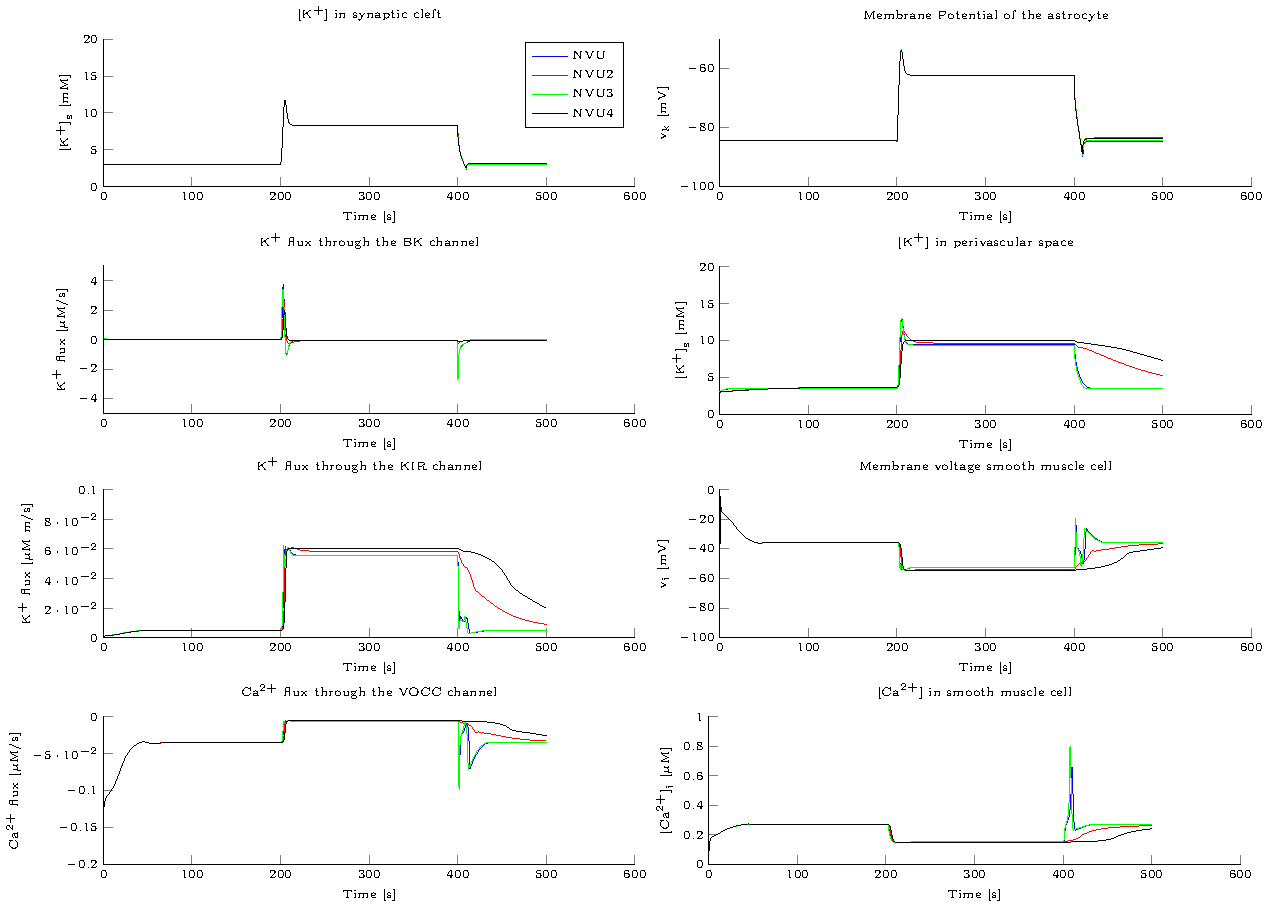
\includegraphics{figures/BK_eff_NVU14.pdf}
			\caption{The effects of different regulation of the BK-channel}
			\label{fig:BKeff}
		\end{figure}
		
		\begin{figure}[h!]
			\centering
			\tiny 
			\setlength\figureheight{7.5 cm} 
			\setlength\figurewidth{18 cm}
			%% % This file was created by matlab2tikz v0.3.3.
% Copyright (c) 2008--2013, Nico Schlömer <nico.schloemer@gmail.com>
% All rights reserved.
% 
% The latest updates can be retrieved from
%   http://www.mathworks.com/matlabcentral/fileexchange/22022-matlab2tikz
% where you can also make suggestions and rate matlab2tikz.
% 
% 
% 
\tiny 
\newlength\figureheight 
\newlength\figurewidth 
\setlength\figureheight{7.5 cm} 
\setlength\figurewidth{18 cm}
\begin{tikzpicture}

\begin{axis}[%
width=\figurewidth,
height=\figureheight,
scale only axis,
xmin=0,
xmax=500,
xlabel={Time [s]},
ymin=14,
ymax=26,
ylabel={$\text{Radius [}\mu\text{m]}$},
title={Radius},
axis x line*=bottom,
axis y line*=left
]
\addplot [
color=blue,
solid,
forget plot
]
table[row sep=crcr]{
0 15\\
0.00089136 15.086742709252\\
0.0017827 15.172090458113\\
0.0026741 15.2560360115582\\
0.0061751 15.573681895346\\
0.0096762 15.8716678008198\\
0.013177 16.1508148929799\\
0.016678 16.4121795826764\\
0.026472 17.0576950285319\\
0.036266 17.5937938309934\\
0.04606 18.0391235161951\\
0.055854 18.4090164535006\\
0.065648 18.7160311907668\\
0.075699 18.9766295873624\\
0.079199 19.0562996982542\\
0.0827 19.1307422642745\\
0.086201 19.200294744483\\
0.089702 19.2652833204659\\
0.093202 19.326004768993\\
0.10095 19.446960384544\\
0.1087 19.5509084703234\\
0.11645 19.6400745467035\\
0.12421 19.7164677533242\\
0.14151 19.8488157649963\\
0.15881 19.9412894717826\\
0.17612 20.0055021499963\\
0.19342 20.0494430051421\\
0.21073 20.0787174306771\\
0.2497 20.1085584745253\\
0.28868 20.1135430665687\\
0.32765 20.1085579496232\\
0.36662 20.0990490799099\\
0.37628 20.0963341308842\\
0.38594 20.0933975140489\\
0.39561 20.0903538270971\\
0.40527 20.0872861657974\\
0.41493 20.0842246119323\\
0.43002 20.0794663927614\\
0.44221 20.0756652698311\\
0.4544 20.0719181692438\\
0.46659 20.0682392448865\\
0.47879 20.0646400616545\\
0.49098 20.061128921923\\
0.51139 20.055461977849\\
0.52695 20.0513304540004\\
0.54251 20.0473670745756\\
0.55807 20.0435743680978\\
0.57363 20.0399536117593\\
0.58919 20.0365050419268\\
0.6088 20.032404176959\\
0.6284 20.028573069082\\
0.64801 20.025008119249\\
0.66761 20.021705022265\\
0.68722 20.018659070354\\
0.73766 20.0119684714242\\
0.78811 20.0068609472821\\
0.83855 20.0032491406767\\
0.889 20.0010475978825\\
0.93944 20.0001745806503\\
1.0031 20.0008482175694\\
1.0667 20.003363640678\\
1.1303 20.0075812478384\\
1.1939 20.0133699844944\\
1.2576 20.0206068859773\\
1.3769 20.0376872232228\\
1.4783 20.0553705492912\\
1.5797 20.0755660621424\\
1.6811 20.0979336020966\\
1.7825 20.1221689069074\\
1.8839 20.1480016500495\\
2.0684 20.1983247524681\\
2.2528 20.2519306454433\\
2.4373 20.3078458548738\\
2.6218 20.3652910024394\\
2.8063 20.4236435434068\\
2.9907 20.4824101996989\\
3.3424 20.5943235866088\\
3.694 20.7044033503508\\
4.0456 20.8113442497274\\
4.3972 20.9143651146193\\
4.7489 21.0129644803024\\
5.2238 21.1385467695008\\
5.6986 21.2549080277067\\
6.1735 21.361781537141\\
6.6484 21.4590826695418\\
7.1233 21.5468266536516\\
7.8241 21.6590746755544\\
8.525 21.7512105449719\\
9.2258 21.8239502616498\\
9.9266 21.8781518395463\\
10.627 21.9148043522122\\
11.627 21.9388105264771\\
12.627 21.9324640998991\\
13.627 21.8992246837436\\
14.627 21.8426677531531\\
15.627 21.7664260346931\\
16.627 21.6741784214251\\
17.627 21.5695393617553\\
18.627 21.4563098278629\\
19.627 21.3376516537362\\
20.627 21.2162642719199\\
21.627 21.094714056133\\
22.627 20.9748177132464\\
23.627 20.8583819755786\\
24.627 20.7464768618656\\
25.627 20.639914505947\\
26.627 20.5389347120455\\
27.627 20.4435956556003\\
28.627 20.3537854589428\\
29.627 20.2692465282273\\
30.627 20.1896878157041\\
31.627 20.1148280682209\\
32.627 20.0443750996855\\
33.627 19.9780154572336\\
34.627 19.9154645348444\\
35.627 19.8564208557801\\
36.627 19.800616844947\\
37.627 19.7477795705695\\
38.627 19.6976804185051\\
39.627 19.6501363939682\\
40.627 19.6050822899162\\
41.627 19.5625505797062\\
42.627 19.5227539982292\\
43.627 19.4861125250299\\
44.627 19.4532360053744\\
45.627 19.4248411502741\\
46.627 19.4016169215688\\
47.627 19.3840599238894\\
48.627 19.3723263299678\\
49.627 19.3661474029747\\
50.627 19.3648387551122\\
51.627 19.3674006888719\\
52.627 19.3726762931689\\
53.627 19.3795183181042\\
54.627 19.386921491385\\
55.627 19.394097662452\\
56.627 19.4004947251505\\
57.627 19.4057757139589\\
58.627 19.4097783030636\\
59.627 19.4124704570767\\
60.627 19.413910922077\\
61.627 19.414217603712\\
62.627 19.4135437893523\\
63.627 19.4120609856897\\
64.627 19.4099468886343\\
65.627 19.4073770798185\\
66.627 19.4045192353998\\
67.627 19.4015288883239\\
68.627 19.3985460800503\\
69.627 19.3956925369754\\
70.627 19.3930692716672\\
71.627 19.3907547076147\\
72.627 19.3888035375176\\
73.627 19.3872465427193\\
74.627 19.3860895875631\\
75.627 19.3853164198701\\
76.627 19.3848972390551\\
77.627 19.3847893480779\\
78.627 19.3849410476232\\
79.627 19.3852953144961\\
80.627 19.3857996870388\\
81.627 19.3863939413772\\
82.627 19.3870241872407\\
83.627 19.3876434762357\\
84.627 19.3882157529703\\
85.627 19.3887143258085\\
86.627 19.3891216571312\\
87.627 19.3894281470544\\
88.627 19.3896326949615\\
89.627 19.389739194341\\
90.627 19.3897556307519\\
91.627 19.3896935098664\\
92.627 19.3895666924924\\
93.627 19.3893903280727\\
94.627 19.3891757584486\\
95.627 19.3889480558901\\
96.627 19.3887213445781\\
97.627 19.3885049933379\\
98.627 19.388306691395\\
99.627 19.3881319278634\\
100.63 19.3879841639529\\
101.63 19.3878649953581\\
102.63 19.3877743963983\\
103.63 19.3877110047444\\
104.63 19.3876724253453\\
105.63 19.3876555327155\\
106.63 19.3876567554654\\
107.63 19.3876723312052\\
108.63 19.3876985240107\\
109.63 19.3877318002628\\
110.63 19.3877689617519\\
111.63 19.3878072374277\\
112.63 19.3878443370625\\
113.63 19.3878784714115\\
114.63 19.3879083442541\\
115.63 19.3879331220536\\
116.63 19.3879523869627\\
117.63 19.3879660786072\\
118.63 19.3879744295744\\
119.63 19.3879778988942\\
120.63 19.3879771070747\\
121.63 19.3879727755084\\
122.63 19.3879656723256\\
123.63 19.3879565660769\\
124.63 19.3879461880021\\
125.63 19.3879352030937\\
126.63 19.387924189712\\
127.63 19.387913627149\\
128.63 19.3879038902708\\
129.63 19.3878952501953\\
130.63 19.3878878798628\\
131.63 19.3878818633347\\
132.63 19.3878772076898\\
133.63 19.3878738564699\\
134.63 19.3878717037431\\
135.63 19.3878706079948\\
136.63 19.3878704052079\\
137.63 19.3878709206501\\
138.63 19.3878719790365\\
139.63 19.3878734128749\\
140.63 19.3878750689228\\
141.63 19.3878768127922\\
142.63 19.3878785318166\\
143.63 19.3878801363615\\
144.63 19.3878815597986\\
145.63 19.3878827573895\\
146.63 19.387883704332\\
147.63 19.3878843932141\\
148.63 19.3878848311081\\
149.63 19.3878850365074\\
150.63 19.3878850362839\\
151.63 19.3878848628048\\
152.63 19.3878845513207\\
153.63 19.3878841376977\\
154.63 19.3878836565402\\
155.63 19.3878831397225\\
156.63 19.3878826153239\\
157.63 19.3878821069443\\
158.63 19.3878816333639\\
159.63 19.3878812084989\\
160.63 19.3878808416013\\
161.63 19.3878805376486\\
162.63 19.387880297869\\
163.63 19.3878801203526\\
164.63 19.3878800007024\\
165.63 19.3878799326874\\
166.63 19.3878799088652\\
167.63 19.3878799211497\\
168.63 19.387879961307\\
169.63 19.3878800213684\\
170.63 19.3878800939559\\
171.63 19.3878801725203\\
172.63 19.3878802514964\\
173.63 19.3878803263841\\
174.63 19.3878803937628\\
175.63 19.3878804512526\\
176.63 19.387880497433\\
177.63 19.3878805317308\\
178.63 19.3878805542885\\
179.63 19.3878805658219\\
180.63 19.3878805674783\\
181.63 19.3878805606984\\
182.63 19.3878805470911\\
183.63 19.3878805283226\\
184.63 19.3878805060237\\
185.63 19.387880481716\\
186.63 19.3878804567568\\
187.63 19.3878804323025\\
188.63 19.3878804092882\\
189.63 19.387880388422\\
190.63 19.3878803701914\\
191.63 19.387880354879\\
192.63 19.3878803425857\\
193.63 19.3878803332582\\
194.63 19.3878803267186\\
195.63 19.3878803226954\\
196.63 19.387880320853\\
197.19 19.387880320475\\
197.62 19.3878803205579\\
197.92 19.3878803207824\\
198.17 19.3878803210569\\
198.37 19.3878803213418\\
198.57 19.3878803216815\\
198.71 19.3878803219504\\
198.85 19.3878803222449\\
198.97 19.3878803225021\\
199.09 19.3878803227749\\
199.21 19.3878803230622\\
199.4 19.3878803235684\\
199.6 19.3878803241092\\
199.8 19.3878803246836\\
199.99 19.3878803252892\\
200.31 19.3878806745814\\
200.54 19.3878819805006\\
200.77 19.3878869247041\\
201.01 19.3879024394529\\
201.24 19.3879439803685\\
201.54 19.3880818647708\\
201.84 19.3884243925259\\
202.14 19.3891906690261\\
202.43 19.3907702110887\\
202.73 19.3938247580976\\
203.03 19.3994289202975\\
203.33 19.4092107196659\\
203.42 19.413249356971\\
203.51 19.4179403944638\\
203.6 19.4233570624364\\
203.69 19.4295686257721\\
203.78 19.4366420253356\\
203.89 19.4469887137542\\
204 19.4589355671239\\
204.12 19.4725597778845\\
204.23 19.4879086988056\\
204.34 19.5050023912354\\
204.53 19.5360841591169\\
204.71 19.5715195247974\\
204.89 19.6111244215684\\
205.08 19.6546564535983\\
205.45 19.7547964860961\\
205.83 19.8677529518062\\
206.2 19.9912202798801\\
206.58 20.1230838625308\\
207.23 20.3651973792844\\
207.87 20.6198001164169\\
208.52 20.8811940924205\\
209.17 21.1451226944319\\
209.82 21.4081188791507\\
210.52 21.6899211759989\\
211.23 21.9635446302252\\
211.93 22.2263565013648\\
212.64 22.4765376922562\\
213.34 22.7129788297538\\
214.34 23.023930654679\\
215.34 23.3060101058857\\
216.34 23.5601845373333\\
217.34 23.7881489552709\\
218.34 23.991859425979\\
219.34 24.1734857959771\\
220.34 24.3346203123536\\
221.34 24.4772383965586\\
222.34 24.6031194144276\\
223.34 24.7137182391122\\
224.34 24.8106143842699\\
225.34 24.8948447768185\\
226.34 24.9674451720932\\
227.34 25.0300420922632\\
228.34 25.0843312706871\\
229.34 25.1311574384076\\
230.34 25.1707570838668\\
231.34 25.2039424898937\\
232.34 25.232317763377\\
233.34 25.2567795563319\\
234.34 25.2773278490748\\
235.34 25.2942983828496\\
236.34 25.3083844922911\\
237.34 25.3202158033602\\
238.34 25.3300961024227\\
239.34 25.3381338804376\\
240.34 25.3444924336183\\
241.34 25.3494476750979\\
242.34 25.3531981336787\\
243.34 25.355983263364\\
244.34 25.3576755513517\\
245.34 25.358422988175\\
246.34 25.3582549268411\\
247.34 25.357594557091\\
248.34 25.3566385339688\\
249.34 25.3552188514419\\
250.34 25.353142601986\\
251.34 25.3504631350426\\
252.34 25.3473944751505\\
253.34 25.344075766978\\
254.34 25.340447702229\\
255.34 25.3365580164363\\
256.34 25.3323986024041\\
257.34 25.3280399605042\\
258.34 25.3235557453584\\
259.34 25.3189950544727\\
260.34 25.3143873262833\\
261.34 25.3097541704684\\
262.34 25.305115800587\\
263.34 25.3004917526476\\
264.34 25.2958994770819\\
265.34 25.2913532986793\\
266.34 25.2868643044155\\
267.34 25.2824407607492\\
268.34 25.2780886153731\\
269.34 25.2738119011719\\
270.34 25.2696130499708\\
271.34 25.2654931704403\\
272.34 25.2614523186466\\
273.34 25.2574897594019\\
274.34 25.2536042054821\\
275.34 25.2497940247954\\
276.34 25.2460574119876\\
277.34 25.2423925252038\\
278.34 25.2387975903569\\
279.34 25.235270975664\\
280.34 25.2318112394603\\
281.34 25.2284171546609\\
282.34 25.2250877135821\\
283.34 25.2218221170136\\
284.34 25.2186197513921\\
285.34 25.2154801577168\\
286.34 25.2124029955086\\
287.34 25.2093880047091\\
288.34 25.206434967959\\
289.34 25.203543675224\\
290.34 25.200713892263\\
291.34 25.1979453339758\\
292.34 25.1952376432508\\
293.34 25.1925903755564\\
294.34 25.1900029892041\\
295.34 25.1874748409486\\
296.34 25.1850051863954\\
297.34 25.1825931845421\\
298.34 25.1802379056971\\
299.34 25.1779383419811\\
300.34 25.1756934196239\\
301.34 25.1735020123089\\
302.34 25.1713629548864\\
303.34 25.1692750568638\\
304.34 25.1672371151794\\
305.34 25.1652479258738\\
306.34 25.1633062943768\\
307.34 25.1614110442278\\
308.34 25.1595610241434\\
309.34 25.1577551134227\\
310.34 25.1559922257547\\
311.34 25.1542713115427\\
312.34 25.1525913589051\\
313.34 25.1509513935383\\
314.34 25.1493504776442\\
315.34 25.1477877081275\\
316.34 25.1462622142654\\
317.34 25.144773155038\\
318.34 25.143319716291\\
319.34 25.1419011078772\\
320.34 25.1405165609022\\
321.34 25.139165325169\\
322.34 25.1378466668956\\
323.34 25.1365598667503\\
324.34 25.1353042182309\\
325.34 25.1340790263924\\
326.34 25.1328836069129\\
327.34 25.1317172854718\\
328.34 25.1305793974082\\
329.34 25.1294692876166\\
330.34 25.1283863106373\\
331.34 25.1273298308948\\
332.34 25.1262992230401\\
333.34 25.1252938723541\\
334.34 25.1243131751768\\
335.34 25.123356539328\\
336.34 25.1224233844929\\
337.34 25.1215131425542\\
338.34 25.1206252578524\\
339.34 25.1197591873682\\
340.34 25.1189144008204\\
341.34 25.1180903806815\\
342.34 25.1172866221125\\
343.34 25.1165026328258\\
344.34 25.1157379328831\\
345.34 25.1149920544402\\
346.34 25.1142645414486\\
347.34 25.1135549493244\\
348.34 25.1128628445977\\
349.34 25.1121878045491\\
350.34 25.111529416845\\
351.34 25.1108872791782\\
352.34 25.1102609989193\\
353.34 25.1096501927859\\
354.34 25.1090544865306\\
355.34 25.1084735146514\\
356.34 25.1079069201258\\
357.34 25.1073543541669\\
358.34 25.1068154760025\\
359.34 25.106289952674\\
360.34 25.1057774588542\\
361.34 25.1052776766812\\
362.34 25.1047902956054\\
363.34 25.104315012248\\
364.34 25.103851530268\\
365.34 25.1033995602343\\
366.34 25.1029588195034\\
367.34 25.1025290320987\\
368.34 25.1021099285905\\
369.34 25.1017012459761\\
370.34 25.1013027275592\\
371.34 25.100914122827\\
372.34 25.1005351873263\\
373.34 25.1001656825377\\
374.34 25.0998053757478\\
375.34 25.0994540399209\\
376.34 25.0991114535695\\
377.34 25.0987774006248\\
378.34 25.0984516703074\\
379.34 25.098134056999\\
380.34 25.0978243601155\\
381.34 25.0975223839821\\
382.34 25.0972279377102\\
383.34 25.096940835078\\
384.34 25.096660894413\\
385.34 25.0963879384783\\
386.34 25.096121794362\\
387.34 25.09586229337\\
388.34 25.0956092709221\\
389.34 25.0953625664516\\
390.34 25.0951220233073\\
391.34 25.0948874886599\\
392.34 25.0946588134101\\
393.34 25.0944358520999\\
394.34 25.0942184628264\\
395.34 25.0940065071583\\
396.34 25.0937998500536\\
397.34 25.0935983597808\\
398.17 25.0934369452003\\
398.58 25.0933569958588\\
398.9 25.0932945878486\\
399.16 25.0932451833328\\
399.42 25.0931960376615\\
399.62 25.0931585101788\\
399.82 25.0931211327314\\
399.88 25.0931092146838\\
399.94 25.0930973111778\\
399.99 25.093089088927\\
400.03 25.0930808727485\\
400.08 25.0930726591664\\
400.15 25.0930592094542\\
400.22 25.0930454736265\\
400.29 25.0930308597443\\
400.36 25.0930141758397\\
400.48 25.0929747831468\\
400.59 25.0929057096635\\
400.71 25.0927797343846\\
400.83 25.0925563520824\\
401.11 25.0910248138135\\
401.23 25.0897407111727\\
401.33 25.0882707110548\\
401.41 25.0867020215159\\
401.5 25.0846906868712\\
401.56 25.0826664897581\\
401.63 25.0801940977795\\
401.66 25.0786504433607\\
401.69 25.0772907811225\\
401.72 25.075805312959\\
401.75 25.0741812907728\\
401.78 25.0724047407577\\
401.81 25.069789118865\\
401.85 25.0668415903166\\
401.89 25.0635230300556\\
401.93 25.0597928682604\\
401.98 25.0536833588353\\
402.03 25.046540041851\\
402.09 25.038247802142\\
402.14 25.0287006091855\\
402.2 25.0178038177857\\
402.37 24.9707115262624\\
402.55 24.9062133117852\\
402.68 24.8491780702569\\
402.81 24.7831133109732\\
402.93 24.7085375848437\\
403.06 24.6261983726885\\
403.27 24.4744927060466\\
403.44 24.3452913596461\\
403.6 24.2089120047494\\
403.77 24.0670889542686\\
403.93 23.9213022399062\\
404.15 23.7243798363228\\
404.37 23.524860023506\\
404.59 23.3244615857513\\
404.81 23.1244563013525\\
405.2 22.7746184998922\\
405.58 22.4317427458578\\
405.97 22.0970807967666\\
406.36 21.7705885991008\\
406.74 21.4514466552498\\
407.4 20.9189931923506\\
408.07 20.3906490768831\\
408.61 19.9423322057\\
409.16 19.4611082667274\\
409.32 19.3064069759506\\
409.48 19.1462049904091\\
409.65 18.9815848611966\\
409.81 18.8152248802248\\
409.97 18.6511126709345\\
410.14 18.4936108968784\\
410.3 18.3445375988908\\
410.47 18.207434357165\\
410.63 18.0826231100055\\
410.8 17.9700258266308\\
410.96 17.869696455081\\
411.13 17.7816893272898\\
411.38 17.6699539601193\\
411.64 17.5856686056412\\
411.89 17.5274497132192\\
412.14 17.4938823954829\\
412.4 17.4832888153517\\
412.65 17.493561654156\\
413.05 17.5454726408614\\
413.31 17.6004991565518\\
413.53 17.6541523200286\\
413.72 17.7088910847332\\
413.89 17.7603946015893\\
414.02 17.8017583412782\\
414.15 17.8443915762949\\
414.28 17.88803669648\\
414.41 17.9324614562631\\
414.63 18.0079751274195\\
414.85 18.0839348875476\\
415.07 18.159781469494\\
415.47 18.2992458711608\\
415.87 18.4353499966224\\
416.28 18.5663969200049\\
416.68 18.6911605356523\\
417.45 18.9080383122005\\
418.22 19.097844206922\\
418.99 19.260441042463\\
419.75 19.3967741989208\\
420.75 19.5391023482347\\
421.75 19.6453375311089\\
422.75 19.7208992229104\\
423.75 19.7708914487207\\
424.75 19.7995486120369\\
425.75 19.8104846210366\\
426.75 19.807026198315\\
427.75 19.7924879295809\\
428.75 19.7690093744546\\
429.75 19.7384635506758\\
430.75 19.7034954457748\\
431.75 19.6665866945986\\
432.75 19.6288976223953\\
433.75 19.591169417408\\
434.75 19.5550175685724\\
435.75 19.5221403795084\\
436.75 19.4929532724304\\
437.75 19.4672320225708\\
438.75 19.4454500462897\\
439.75 19.4282386662642\\
440.75 19.4151194458624\\
441.75 19.4050219495022\\
442.75 19.3976044810698\\
443.75 19.3929477874565\\
444.75 19.3904109677088\\
445.75 19.38893896785\\
446.75 19.3881916659342\\
447.75 19.3883472592417\\
448.75 19.3890699390866\\
449.75 19.389655519191\\
450.75 19.3899938206318\\
451.75 19.3904634716546\\
452.75 19.3910085964348\\
453.75 19.3910865136071\\
454.75 19.3909471442392\\
455.75 19.3907410072337\\
456.75 19.3904188739478\\
457.75 19.3899359151219\\
458.75 19.3893497329636\\
459.75 19.3887409512908\\
460.75 19.388141642022\\
461.75 19.3875595069127\\
462.75 19.3870064676383\\
463.75 19.3865008846619\\
464.75 19.3860572463003\\
465.75 19.3856860740647\\
466.75 19.385393853132\\
467.75 19.3851790882215\\
468.75 19.3850345948338\\
469.75 19.384960063575\\
470.75 19.3849530612084\\
471.75 19.3849995766869\\
472.75 19.38508221456\\
473.75 19.3851842333959\\
474.75 19.3852988710469\\
475.75 19.3854175727562\\
476.75 19.385533424526\\
477.75 19.3856413834398\\
478.75 19.3857377091787\\
479.75 19.3858197244884\\
480.75 19.3858858224938\\
481.75 19.3859354575653\\
482.75 19.385969034338\\
483.75 19.3859877256613\\
484.75 19.385993266\\
485.75 19.3859877491326\\
486.75 19.3859734449398\\
487.75 19.3859526434831\\
488.75 19.3859275306906\\
489.75 19.3859000965163\\
490.75 19.3858720735479\\
491.75 19.3858449021928\\
492.75 19.3858197177758\\
493.75 19.3857973548709\\
494.75 19.3857783646069\\
495.75 19.3857630412893\\
496.75 19.3857514552864\\
497.75 19.3857434896658\\
498.75 19.3857388784921\\
499.75 19.385737245032\\
500 19.3857373914139\\
};
\addplot [
color=red,
solid,
forget plot
]
table[row sep=crcr]{
0 15\\
0.0011996 15.1161805502527\\
0.0023992 15.2298584170436\\
0.0035988 15.3410341294794\\
0.0085566 15.7772072413411\\
0.013514 16.1756295425181\\
0.018472 16.5387970912678\\
0.02343 16.8695723485373\\
0.033542 17.4547692163756\\
0.043655 17.9375277882318\\
0.053767 18.3359607228358\\
0.063879 18.6647507175825\\
0.073991 18.9358256164481\\
0.084819 19.173195698794\\
0.095647 19.365711012369\\
0.10647 19.5216207440694\\
0.1173 19.6476547999014\\
0.12813 19.7493072513544\\
0.14659 19.8782322752756\\
0.16505 19.9662251432372\\
0.18351 20.025636383493\\
0.20197 20.0648863303133\\
0.22042 20.0898669455215\\
0.26398 20.1120080420028\\
0.30753 20.1109753818855\\
0.35108 20.1022669734003\\
0.37397 20.0967184922077\\
0.38969 20.0921285120397\\
0.4054 20.0871946040087\\
0.42111 20.0821975323318\\
0.43393 20.0781719370309\\
0.44676 20.0742066635754\\
0.45959 20.0703061000371\\
0.47242 20.0664815819863\\
0.48525 20.0627463882537\\
0.50035 20.0584783334007\\
0.51544 20.0543584019034\\
0.53054 20.0503928045309\\
0.54564 20.0465852944249\\
0.56073 20.042938159938\\
0.57728 20.0391275719509\\
0.59382 20.0355111064013\\
0.61036 20.0320878487165\\
0.6269 20.0288561663812\\
0.64344 20.0258139554692\\
0.65998 20.0229587677075\\
0.69992 20.0168192246474\\
0.73986 20.0117126463781\\
0.77979 20.0075957732113\\
0.81973 20.0044248763385\\
0.85967 20.0021572524085\\
0.99616 20.000457706077\\
1.1327 20.0073252849047\\
1.2692 20.0214732343814\\
1.4056 20.0417229298793\\
1.6062 20.0805572215394\\
1.8067 20.1276838409425\\
2.0072 20.1808325567649\\
2.2078 20.2382631920915\\
2.4083 20.2986461029279\\
2.8551 20.4393554150949\\
3.302 20.5818993132103\\
3.7488 20.7215356891832\\
4.1956 20.8558705328006\\
4.6425 20.9835750714452\\
5.3586 21.1725284734544\\
6.0748 21.3402981144615\\
6.791 21.4862476267052\\
7.5072 21.6104851255871\\
8.2234 21.7134027093416\\
9.2234 21.8227540001375\\
10.223 21.8943929910369\\
11.223 21.9312688319175\\
12.223 21.9363825147715\\
12.523 21.9321915110584\\
12.823 21.9255199341992\\
13.123 21.9164652218713\\
13.423 21.9051358028365\\
13.513 21.9013097672706\\
13.603 21.8972914215106\\
13.693 21.8930831355345\\
13.783 21.8886874571793\\
13.873 21.8841070706287\\
13.929 21.8811943943803\\
13.948 21.8801847773099\\
13.967 21.8791672124993\\
13.986 21.8781417241817\\
14.004 21.8771083370197\\
14.023 21.8760670757882\\
14.079 21.8729878335937\\
14.134 21.8698425362044\\
14.189 21.8666317945724\\
14.244 21.863356219857\\
14.299 21.8600164236038\\
14.354 21.8566130176879\\
14.409 21.8531466142535\\
14.465 21.8496178257032\\
14.52 21.8460093123946\\
14.575 21.8423390347355\\
14.631 21.8386076150283\\
14.686 21.8348156758061\\
14.742 21.8309638398587\\
14.811 21.8260543913022\\
14.88 21.821053127418\\
14.95 21.8159612755678\\
15.019 21.8107800644145\\
15.089 21.8055107240197\\
15.202 21.7967518600676\\
15.315 21.7877682533352\\
15.428 21.778565221909\\
15.541 21.7691480877588\\
15.654 21.7595221725314\\
15.804 21.7464025079848\\
15.954 21.73293527296\\
16.104 21.7191329226297\\
16.255 21.7050078648933\\
16.405 21.6905724537721\\
16.675 21.6638462809679\\
16.946 21.6362255887758\\
17.216 21.6077808795258\\
17.487 21.5785818671927\\
17.757 21.5486973595461\\
18.061 21.514453823533\\
18.364 21.4795271422514\\
18.667 21.4440088125734\\
18.971 21.407987846917\\
19.274 21.3715504955187\\
19.375 21.3593681565706\\
19.476 21.3471520158111\\
19.576 21.3349050273697\\
19.677 21.3226301082263\\
19.778 21.3103301117227\\
19.938 21.2907978554783\\
20.097 21.2712205938031\\
20.257 21.2516089838392\\
20.416 21.2319733778766\\
20.576 21.2123238211441\\
20.994 21.1609752552639\\
21.411 21.1097606796826\\
21.828 21.0588233082023\\
22.056 21.0312292410574\\
22.119 21.0235290298314\\
22.183 21.0158408229094\\
22.247 21.0081647905315\\
22.31 21.0005012205231\\
22.432 20.9858679743007\\
22.554 20.9712841972909\\
22.676 20.9567524450792\\
22.798 20.9422751566464\\
22.92 20.9278546274224\\
23.367 20.8754517291492\\
23.684 20.8388890006314\\
24 20.8027981632002\\
24.242 20.7755436532105\\
24.484 20.7485893776656\\
24.726 20.721943430108\\
24.968 20.6956125468695\\
25.298 20.6602281701798\\
25.628 20.6254507433642\\
25.958 20.591288799648\\
26.288 20.5577474585252\\
26.618 20.5248288552843\\
27.087 20.4790855852406\\
27.556 20.4345934058901\\
28.025 20.391338320056\\
28.494 20.3493006535569\\
28.964 20.3084566104045\\
29.615 20.2536869647747\\
30.266 20.2010847578641\\
30.917 20.1505693733169\\
31.569 20.1020577887108\\
32.372 20.0448555544429\\
33.175 19.9904262409745\\
33.979 19.9386139104578\\
34.782 19.8892673566781\\
35.586 19.8422389543998\\
36.23 19.8060741112901\\
36.875 19.7712273813817\\
37.52 19.7376314004941\\
38.164 19.7052213073229\\
38.969 19.6663400642168\\
39.774 19.6291357475768\\
40.579 19.5935640764412\\
41.384 19.559646301997\\
42.189 19.5274931242759\\
43.189 19.4902783119528\\
44.189 19.4566063522246\\
45.189 19.4271476403952\\
46.189 19.4025936248862\\
47.189 19.3835178886192\\
48.189 19.370210639415\\
49.189 19.3625605489187\\
50.189 19.3599250013312\\
51.189 19.3614440290381\\
52.189 19.3660772299508\\
53.189 19.3727312465224\\
54.189 19.3803781324795\\
55.189 19.3881508303778\\
56.189 19.395392466716\\
57.189 19.4016654067198\\
58.189 19.4067264842922\\
59.189 19.4104615196022\\
60.189 19.4129053322707\\
61.189 19.4141234719111\\
62.189 19.4143082482514\\
63.189 19.4136109053107\\
64.189 19.4121857287602\\
65.189 19.4102038807367\\
66.189 19.4078389605934\\
67.189 19.4052752970001\\
68.189 19.4026049368187\\
69.189 19.4000589034798\\
70.189 19.3977244537405\\
71.189 19.395676501626\\
72.189 19.3939019374305\\
73.189 19.3924650958731\\
74.189 19.3914003801225\\
75.189 19.390728698553\\
76.189 19.3904999693943\\
77.189 19.3905908429322\\
78.189 19.3909202956459\\
79.189 19.3914307718201\\
80.189 19.3920713647786\\
81.189 19.3928100240917\\
82.189 19.3935735447537\\
83.189 19.3943567759723\\
84.189 19.3951201688979\\
85.189 19.3958424539673\\
86.189 19.3964740728047\\
87.189 19.3970062223538\\
88.189 19.3974696516376\\
89.189 19.3978467965107\\
90.189 19.3981504443508\\
91.189 19.3983804605394\\
92.189 19.3985461426205\\
93.189 19.3986557755954\\
94.189 19.3987200156979\\
95.189 19.3987513143906\\
96.189 19.398760752259\\
97.189 19.3987611227735\\
98.189 19.3987613039646\\
99.189 19.3987715274528\\
100.19 19.3987965266004\\
101.19 19.3988426995002\\
102.19 19.3989101702127\\
103.19 19.3990018041004\\
104.19 19.3991139304827\\
105.19 19.3992511773246\\
106.19 19.399401545882\\
107.19 19.3995660984847\\
108.19 19.3997382033307\\
109.19 19.3999151590558\\
110.19 19.4000931782311\\
111.19 19.4002694144783\\
112.19 19.4004419522427\\
113.19 19.4006086466064\\
114.19 19.4007689425303\\
115.19 19.4009214181517\\
116.19 19.40106653635\\
117.19 19.4012034058705\\
118.19 19.4013332569322\\
119.19 19.4014554928876\\
120.19 19.4015719082653\\
121.19 19.4016819587131\\
122.19 19.4017878296495\\
123.19 19.401890608268\\
124.19 19.4019891786381\\
125.19 19.4020861082237\\
126.19 19.402180396825\\
127.19 19.4022731619239\\
128.19 19.4023642254809\\
129.19 19.4024542171883\\
130.19 19.4025431444149\\
131.19 19.4026314210451\\
132.19 19.4027189711234\\
133.19 19.4028060395103\\
134.19 19.4028923853421\\
135.19 19.4029781361583\\
136.19 19.4030629104484\\
137.19 19.4031468017024\\
138.19 19.4032293500402\\
139.19 19.4033106982696\\
140.19 19.4033903600714\\
141.19 19.4034685862658\\
142.19 19.4035448850379\\
143.19 19.4036196440806\\
144.19 19.4036923569123\\
145.19 19.4037635557801\\
146.19 19.4038326907289\\
147.19 19.4039004376837\\
148.19 19.4039661655335\\
149.19 19.4040306945721\\
150.19 19.4040932727202\\
151.19 19.4041548726605\\
152.19 19.4042145818568\\
153.19 19.4042735430789\\
154.19 19.4043306437996\\
155.19 19.4043872248806\\
156.19 19.4044419325301\\
157.19 19.4044963441747\\
158.19 19.4045503738259\\
159.19 19.4046031971564\\
160.19 19.4046554631632\\
161.19 19.4047063680818\\
162.19 19.4047561308048\\
163.19 19.4048043913832\\
164.19 19.4048513816306\\
165.19 19.4048969733521\\
166.19 19.4049414817693\\
167.19 19.4049848273907\\
168.19 19.4050273455672\\
169.19 19.4050688960095\\
170.19 19.40510980045\\
171.19 19.405149823224\\
172.19 19.4051892867019\\
173.19 19.4052278667783\\
174.19 19.4052659214024\\
175.19 19.4053030517525\\
176.19 19.4053396839865\\
177.19 19.4053753469521\\
178.19 19.4054105575893\\
179.19 19.4054447609152\\
180.19 19.4054785804773\\
181.19 19.4055113567786\\
182.19 19.4055438356322\\
183.19 19.405575228053\\
184.19 19.4056064224515\\
185.19 19.405636473078\\
186.19 19.4056664378955\\
187.19 19.4056951840474\\
188.19 19.4057239727876\\
189.19 19.4057514486815\\
190.19 19.4057791166916\\
191.19 19.4058068234386\\
192.19 19.4058339075736\\
193.19 19.4058607939657\\
194.19 19.4058868130861\\
195.19 19.4059120444841\\
196.19 19.4059362233477\\
196.81 19.4059506932817\\
197.25 19.4059608485202\\
197.57 19.4059681725378\\
197.82 19.4059738787083\\
198.03 19.4059784767197\\
198.24 19.4059830383396\\
198.38 19.4059861346842\\
198.52 19.4059892141444\\
198.63 19.4059916372274\\
198.74 19.4059940496131\\
198.83 19.4059960200086\\
198.92 19.4059979829372\\
199.01 19.4059999382165\\
199.17 19.4060031720059\\
199.32 19.4060063839156\\
199.47 19.4060095710466\\
199.62 19.4060127301919\\
199.84 19.4060172871953\\
200.07 19.4060217576806\\
200.29 19.4060261114475\\
200.51 19.4060303119587\\
200.69 19.4060336328008\\
200.87 19.4060369346796\\
201.05 19.4060405112389\\
201.23 19.4060450440795\\
201.42 19.4060518535005\\
201.6 19.4060634940395\\
201.79 19.4060838345699\\
201.97 19.4061190946904\\
202.15 19.406178734046\\
202.34 19.4062767913841\\
202.63 19.4065660709956\\
202.92 19.4071387899357\\
203.21 19.4082132143256\\
203.5 19.4101408404325\\
203.79 19.4134629350913\\
204.09 19.4192398849599\\
204.39 19.4286164476247\\
204.69 19.4432046638235\\
204.94 19.4604070147608\\
205.19 19.4835078429698\\
205.44 19.5134720624616\\
205.68 19.5509842813481\\
205.85 19.5811047870655\\
206.02 19.6148697725403\\
206.19 19.6521940711919\\
206.36 19.6929456100603\\
206.6 19.7564571612159\\
206.84 19.8259943729643\\
207.08 19.9009611162443\\
207.32 19.9807371037646\\
207.65 20.097983746358\\
207.99 20.2217864966869\\
208.32 20.3506854634512\\
208.65 20.4834050888119\\
208.99 20.6188497713501\\
209.66 20.8991489757025\\
210.18 21.1150185011729\\
210.7 21.3294877625089\\
211.22 21.5410182440793\\
211.74 21.7484166470685\\
212.26 21.9507597005762\\
212.9 22.1928981909134\\
213.54 22.4253778177878\\
214.18 22.6476261907193\\
214.82 22.8593234658572\\
215.46 23.0603276306025\\
216.16 23.2685648670087\\
216.87 23.4640308240348\\
217.57 23.6469608418441\\
218.27 23.8176752162005\\
218.98 23.9765418262423\\
219.98 24.182932640638\\
220.98 24.3676496308881\\
221.98 24.5321444060175\\
222.98 24.6778919619077\\
223.98 24.8064440188195\\
224.98 24.9192677723096\\
225.98 25.0180049200459\\
226.98 25.1037263365759\\
227.98 25.1783852229027\\
228.98 25.2429450268746\\
229.98 25.2983451811971\\
230.98 25.3455996618169\\
231.98 25.3858945687386\\
232.98 25.4203321006627\\
233.98 25.4496078831438\\
234.98 25.4742815156883\\
235.98 25.4949981818167\\
236.98 25.5125898491784\\
237.98 25.5276929860253\\
238.98 25.5406223525692\\
239.98 25.5509336892167\\
240.98 25.5597902789409\\
241.98 25.5670300765348\\
242.98 25.5727741713406\\
243.98 25.5772757036113\\
244.98 25.5807754968568\\
245.98 25.5834370014661\\
246.98 25.5853509790604\\
247.98 25.5865695594943\\
248.98 25.5871368794087\\
249.98 25.587103349443\\
250.98 25.5865261514534\\
251.98 25.585463931508\\
252.98 25.5839720720957\\
253.98 25.5821008847414\\
254.98 25.5798961768998\\
255.98 25.5774006225581\\
256.98 25.574654787464\\
257.98 25.5716974244216\\
258.98 25.5685652342803\\
259.98 25.5652924390501\\
260.98 25.5619104302464\\
261.98 25.5584475799872\\
262.98 25.5549291958674\\
263.98 25.5513775591169\\
264.98 25.5478120058193\\
265.98 25.5442490349408\\
266.98 25.5407024475544\\
267.98 25.537183521817\\
268.98 25.5337012243897\\
269.98 25.530262450193\\
270.98 25.5268722797893\\
271.98 25.5235342421205\\
272.98 25.5202505731044\\
273.98 25.5170224621403\\
274.98 25.513850281301\\
275.98 25.5107337928998\\
276.98 25.5076723328146\\
277.98 25.5046649675831\\
278.98 25.5017106247456\\
279.98 25.4988081966137\\
280.98 25.4959566188692\\
281.98 25.493154925881\\
282.98 25.4904022854017\\
283.98 25.4876980154347\\
284.98 25.4850415864139\\
285.98 25.4824326116866\\
286.98 25.4798708293456\\
287.98 25.4773560781191\\
288.98 25.4748882698828\\
289.98 25.4724673609204\\
290.98 25.4700933238021\\
291.98 25.4677661212881\\
292.98 25.465485683379\\
293.98 25.4632518882124\\
294.98 25.4610645472532\\
295.98 25.4589233948853\\
296.98 25.4568280823295\\
297.98 25.4547781755736\\
298.98 25.4527731569004\\
299.98 25.4508124294605\\
300.98 25.4488953243144\\
301.98 25.4470211093145\\
302.98 25.4451889992379\\
303.98 25.4433981665889\\
304.98 25.4416477525719\\
305.98 25.4399368777791\\
306.98 25.438264652241\\
307.98 25.4366301845436\\
308.98 25.4350325898211\\
309.98 25.4334709964893\\
310.98 25.4319445516706\\
311.98 25.4304524253118\\
312.98 25.4289938130552\\
313.98 25.4275679379583\\
314.98 25.426174051193\\
315.98 25.4248114318701\\
316.98 25.4234793861507\\
317.98 25.4221772458038\\
318.98 25.4209043663688\\
319.98 25.4196601250674\\
320.98 25.4184439185976\\
321.98 25.4172551609236\\
322.98 25.4160932811545\\
323.98 25.414957721587\\
324.98 25.4138479359657\\
325.98 25.4127633879945\\
326.98 25.4117035501194\\
327.98 25.410667902584\\
328.98 25.4096559327482\\
329.98 25.4086671346504\\
330.98 25.4077010087867\\
331.98 25.4067570620736\\
332.98 25.4058348079609\\
333.98 25.404933766657\\
334.98 25.4040534654345\\
335.98 25.4031934389806\\
336.98 25.4023532297657\\
337.98 25.4015323884035\\
338.98 25.4007304739822\\
339.98 25.399947054352\\
340.98 25.399181706355\\
341.98 25.398434015993\\
342.98 25.3977035785283\\
343.98 25.3969899985182\\
344.98 25.3962928897862\\
345.98 25.3956118753354\\
346.98 25.3949465872105\\
347.98 25.3942966663174\\
348.98 25.3936617622076\\
349.98 25.3930415328379\\
350.98 25.3924356443123\\
351.98 25.3918437706147\\
352.98 25.3912655933398\\
353.98 25.390700801427\\
354.98 25.3901490909038\\
355.98 25.3896101646412\\
356.98 25.3890837321254\\
357.98 25.3885695092453\\
358.98 25.3880672180991\\
359.98 25.3875765868185\\
360.98 25.3870973494093\\
361.98 25.3866292456095\\
362.98 25.3861720207606\\
363.98 25.3857254256915\\
364.98 25.385289216614\\
365.98 25.3848631550252\\
366.98 25.3844470076175\\
367.98 25.3840405461929\\
368.98 25.3836435475805\\
369.98 25.383255793555\\
370.98 25.3828770707564\\
371.98 25.3825071706088\\
372.98 25.382145889238\\
373.98 25.3817930273878\\
374.98 25.3814483903342\\
375.98 25.3811117877987\\
376.98 25.3807830338585\\
377.98 25.3804619468568\\
378.98 25.3801483493115\\
379.98 25.379842067823\\
380.98 25.3795429329824\\
381.98 25.3792507792801\\
382.98 25.3789654450145\\
383.98 25.3786867722023\\
384.98 25.3784146064903\\
385.98 25.378148797069\\
386.98 25.3778891965881\\
387.98 25.3776356610742\\
388.98 25.377388049851\\
389.98 25.3771462254619\\
390.98 25.3769100535944\\
391.98 25.3766794030074\\
392.98 25.3764541454549\\
393.98 25.3762341555805\\
394.98 25.3760193105718\\
395.98 25.3758094880308\\
396.98 25.3756045506825\\
397.98 25.3754058975722\\
398.44 25.3753159341991\\
398.8 25.3752455332597\\
399.07 25.3751918239614\\
399.35 25.3751384496941\\
399.55 25.3750997352288\\
399.76 25.3750612654506\\
399.96 25.3750230994805\\
400.26 25.3749673599021\\
400.34 25.3749503699029\\
400.43 25.3749329376281\\
400.52 25.3749147788256\\
400.61 25.3748954741441\\
400.92 25.3747982337044\\
401.24 25.3746228524926\\
401.56 25.374300683026\\
401.87 25.3737445418088\\
402.11 25.3731112083021\\
402.35 25.372240407079\\
402.59 25.3710864054924\\
402.83 25.3696054532532\\
403.14 25.3671386329977\\
403.45 25.3639759848091\\
403.77 25.3600446822439\\
404.08 25.3552862768042\\
404.39 25.3496570233513\\
404.93 25.3376627985525\\
405.47 25.3228521964441\\
406.02 25.3052444344809\\
406.56 25.2849456996663\\
407.1 25.2621263109036\\
408.1 25.2142945744546\\
408.77 25.1789544021278\\
409.43 25.1414585110522\\
410.1 25.1024204572395\\
410.61 25.0716533377852\\
411.12 25.0405340894467\\
411.63 25.0091666281475\\
412.15 24.9775115318429\\
412.66 24.9454011555596\\
413.31 24.9037286144152\\
413.95 24.860180024205\\
414.6 24.8139894887496\\
415.25 24.7643501549197\\
415.9 24.7104203763176\\
416.77 24.6289713064621\\
417.65 24.5354765110595\\
418.52 24.4270815966493\\
419.4 24.3007959264512\\
420.28 24.1543781589572\\
421.2 23.9786731270867\\
422.12 23.7857556134422\\
423.04 23.5855010170839\\
423.96 23.3889740380897\\
424.89 23.2030165260016\\
425.81 23.0282331797987\\
426.73 22.8604137347416\\
427.68 22.6903856999802\\
428.64 22.5242747297274\\
429.59 22.3645182132698\\
430.55 22.213123812856\\
431.5 22.0702787499143\\
432.5 21.9285346741372\\
433.5 21.7936768764955\\
434.5 21.6654133731648\\
435.5 21.5442062168326\\
436.5 21.4302474564293\\
437.5 21.3232947777116\\
438.5 21.2227350557172\\
439.5 21.1281913701816\\
440.5 21.0394464000326\\
441.5 20.9565187661476\\
442.5 20.8792252088331\\
443.5 20.8085138888477\\
444.5 20.7429472698168\\
445.5 20.6819529007471\\
446.5 20.6252136726278\\
447.5 20.5724103543424\\
448.5 20.522554509157\\
449.5 20.4759228415012\\
450.5 20.4324199751863\\
451.5 20.391896223489\\
452.5 20.3541170259888\\
453.5 20.3188483389164\\
454.5 20.2858560853627\\
455.5 20.2549221104205\\
456.5 20.2258433159042\\
457.5 20.1984359440509\\
458.5 20.1725351887119\\
459.5 20.1479954400529\\
460.5 20.124688661961\\
461.5 20.1025028837337\\
462.5 20.0813402289233\\
463.5 20.0611152020974\\
464.5 20.0417530088194\\
465.5 20.0231881285351\\
466.5 20.0053630199769\\
467.5 19.9882270207975\\
468.5 19.971735376533\\
469.5 19.9558484134538\\
470.5 19.9405308181267\\
471.5 19.9257510229592\\
472.5 19.9114806747457\\
473.5 19.8976941810459\\
474.5 19.8843683196756\\
475.5 19.8714819056452\\
476.5 19.8590155057905\\
477.5 19.8469511961611\\
478.5 19.8352723553993\\
479.5 19.823963490145\\
480.5 19.8130100876086\\
481.5 19.8023984921771\\
482.5 19.7921158024756\\
483.5 19.7821497863147\\
484.5 19.7724888107833\\
485.5 19.7631217852924\\
486.5 19.7540381153691\\
487.5 19.7452276653464\\
488.5 19.7366807281512\\
489.5 19.7283880007177\\
490.5 19.7203405636205\\
491.5 19.7125298638521\\
492.5 19.7049476997517\\
493.5 19.697586207365\\
494.5 19.6904378476421\\
495.5 19.6834953940427\\
496.5 19.676751920277\\
497.5 19.6702007879929\\
498.5 19.6638356343441\\
499.5 19.6576503594457\\
500 19.6546336422684\\
};
\addplot [
color=green,
solid,
forget plot
]
table[row sep=crcr]{
0 15\\
0.00089136 15.086742709252\\
0.0017827 15.172090458113\\
0.0026741 15.2560360115582\\
0.0061751 15.573681895346\\
0.0096762 15.8716678008198\\
0.013177 16.1508148929799\\
0.016678 16.4121795826764\\
0.026472 17.0576950279345\\
0.036266 17.5937938300017\\
0.04606 18.0391235149603\\
0.055854 18.4090164521342\\
0.065648 18.7160311893499\\
0.075699 18.9766295862787\\
0.079199 19.0562996972764\\
0.0827 19.1307422633937\\
0.086201 19.2002947436907\\
0.089702 19.2652833197545\\
0.093202 19.3260047683553\\
0.10095 19.4469603840256\\
0.1087 19.5509084699038\\
0.11645 19.6400745463655\\
0.12421 19.7164677530532\\
0.14151 19.8488157641591\\
0.15881 19.9412894707533\\
0.17612 20.0055021489797\\
0.19342 20.0494430042441\\
0.21073 20.078717429946\\
0.2497 20.1085584749735\\
0.28868 20.1135430654727\\
0.32765 20.1085579468218\\
0.36662 20.0990490753656\\
0.37628 20.096334395124\\
0.38594 20.0933980726962\\
0.3956 20.0903546909521\\
0.40526 20.0872873337735\\
0.41492 20.0842260774152\\
0.43001 20.0794691442801\\
0.4422 20.0756682312424\\
0.45439 20.071921321103\\
0.46658 20.0682425683797\\
0.47877 20.0646435381978\\
0.49097 20.0611325332704\\
0.51138 20.0554653970622\\
0.52694 20.0513337902322\\
0.5425 20.0473703200274\\
0.55806 20.0435775162883\\
0.57362 20.0399566572402\\
0.58918 20.0365079800681\\
0.60878 20.0324069725467\\
0.62839 20.0285757169916\\
0.64799 20.0250106150851\\
0.6676 20.021707362173\\
0.6872 20.0186612508985\\
0.73765 20.0119703145765\\
0.78809 20.0068623914478\\
0.83854 20.003250131018\\
0.88898 20.0010480853741\\
0.93942 20.0001745215748\\
1.071 20.0036075846413\\
1.2025 20.0142948050527\\
1.3341 20.0311110545021\\
1.4657 20.0530778687687\\
1.5972 20.0793456118078\\
1.8941 20.1509475597402\\
2.191 20.2341419485569\\
2.4879 20.3240366315015\\
2.7847 20.4173505613767\\
3.0816 20.5118736712578\\
3.4058 20.6147076339536\\
3.73 20.7157751130597\\
4.0542 20.814139056639\\
4.3784 20.9091807252326\\
4.7026 21.0004850119055\\
5.1806 21.1277477206733\\
5.6586 21.2457075306458\\
6.1367 21.354071441259\\
6.6147 21.4527400858358\\
7.0927 21.5417223177979\\
7.8129 21.6577215042994\\
8.5332 21.7524680045887\\
9.2535 21.826740838818\\
9.9737 21.881480665322\\
10.694 21.9177415776813\\
11.694 21.9396101533741\\
12.694 21.9313532553638\\
13.694 21.8964359361749\\
14.694 21.8384314161615\\
15.694 21.7609973037053\\
16.694 21.6681338977109\\
17.694 21.5632489029739\\
18.694 21.4496713979599\\
19.694 21.3306099948971\\
20.694 21.2088039084783\\
21.694 21.0868439244776\\
22.694 20.9669121535024\\
23.694 20.8506167789265\\
24.694 20.739060123804\\
25.694 20.6328977143517\\
26.694 20.5323329624598\\
27.694 20.4373209146014\\
28.694 20.3477332341066\\
29.694 20.2634334064\\
30.694 20.1841964913231\\
31.694 20.1096705455744\\
32.694 20.0394583290971\\
33.694 19.9732286451362\\
34.694 19.9107427859714\\
35.694 19.8517964115441\\
36.694 19.7961512761848\\
37.694 19.7434898103217\\
38.694 19.6935387599716\\
39.694 19.6461219556297\\
40.694 19.6011891438513\\
41.694 19.5588230286541\\
42.694 19.5192606687834\\
43.694 19.4829241526445\\
44.694 19.4504176611828\\
45.694 19.4224537264499\\
46.694 19.3997111857891\\
47.694 19.382668470794\\
48.694 19.3713459531005\\
49.694 19.3653863805698\\
50.694 19.3641237235899\\
51.694 19.3666202090054\\
52.694 19.3718001088772\\
53.694 19.3785791363499\\
54.694 19.3859835513315\\
55.694 19.39322504819\\
56.694 19.3997316861235\\
57.694 19.4051406980031\\
58.694 19.4092681461244\\
59.694 19.412068695063\\
60.694 19.4135956470769\\
61.694 19.4139666900846\\
62.694 19.4133373572285\\
63.694 19.4118819035774\\
64.694 19.4097609617733\\
65.694 19.4071647152434\\
66.694 19.4042675888187\\
67.694 19.4012344815706\\
68.694 19.3982055321033\\
69.694 19.3953032521423\\
70.694 19.3926282631495\\
71.694 19.3902610662464\\
72.694 19.3882586735052\\
73.694 19.3866552490557\\
74.694 19.3854561689866\\
75.694 19.3846488346684\\
76.694 19.3842056225634\\
77.694 19.3840844274087\\
78.694 19.3842329452482\\
79.694 19.3845927054477\\
80.694 19.3851034953736\\
81.694 19.3857071309543\\
82.694 19.3863461650622\\
83.694 19.3869593913005\\
84.694 19.387516873273\\
85.694 19.3879984330168\\
86.694 19.3883911228136\\
87.694 19.3887096403632\\
88.694 19.3889378930327\\
89.694 19.3890737906067\\
90.694 19.3891202068862\\
91.694 19.3890869272136\\
92.694 19.3889867321244\\
93.694 19.3888342793665\\
94.694 19.3886394827868\\
95.694 19.388427436234\\
96.694 19.3882125506234\\
97.694 19.3880038730206\\
98.694 19.3878094290119\\
99.694 19.3876351752976\\
100.69 19.3874851845793\\
101.69 19.3873617081274\\
102.69 19.387265365924\\
103.69 19.387195388365\\
104.69 19.3871498940022\\
105.69 19.3871261782089\\
106.69 19.3871209941008\\
107.69 19.3871308110536\\
108.69 19.3871520406489\\
109.69 19.387181223896\\
110.69 19.3872151770825\\
111.69 19.3872510964837\\
112.69 19.3872866243839\\
113.69 19.3873198804609\\
114.69 19.3873494636053\\
115.69 19.3873744297672\\
116.69 19.3873942515397\\
117.69 19.3874087649766\\
118.69 19.3874181086965\\
119.69 19.3874226597194\\
120.69 19.3874229697766\\
121.69 19.3874197050944\\
122.69 19.3874135919083\\
123.69 19.387405369264\\
124.69 19.3873957500183\\
125.69 19.3873853903904\\
126.69 19.3873748679428\\
127.69 19.3873646674876\\
128.69 19.3873551741343\\
129.69 19.3873466724911\\
130.69 19.3873393509257\\
131.69 19.3873333097435\\
132.69 19.3873285721665\\
133.69 19.3873250970628\\
134.69 19.3873227924868\\
135.69 19.3873215292219\\
136.69 19.3873211536656\\
137.69 19.3873214995517\\
138.69 19.3873223981505\\
139.69 19.3873236867315\\
140.69 19.3873252151936\\
141.69 19.3873268508787\\
142.69 19.3873284816648\\
143.69 19.3873300175064\\
144.69 19.3873313906307\\
145.69 19.3873325546267\\
146.69 19.387333482674\\
147.69 19.3873341651558\\
148.69 19.3873346068837\\
149.69 19.3873348241401\\
150.69 19.3873348417142\\
151.69 19.3873346900774\\
152.69 19.3873344028071\\
153.69 19.3873340143393\\
154.69 19.3873335580971\\
155.69 19.3873330650169\\
156.69 19.3873325624699\\
157.69 19.3873320735584\\
158.69 19.3873316167518\\
159.69 19.3873312058165\\
160.69 19.3873308499901\\
161.69 19.3873305543451\\
162.69 19.3873303202896\\
163.69 19.3873301461561\\
164.69 19.3873300278323\\
165.69 19.3873299593959\\
166.69 19.3873299337223\\
167.69 19.3873299430398\\
168.69 19.3873299794147\\
169.69 19.3873300351565\\
170.69 19.3873301031377\\
171.69 19.3873301770278\\
172.69 19.3873302514465\\
173.69 19.3873303220434\\
174.69 19.3873303855137\\
175.69 19.3873304395603\\
176.69 19.3873304828151\\
177.69 19.3873305147301\\
178.69 19.3873305354484\\
179.69 19.387330545667\\
180.69 19.3873305464972\\
181.69 19.3873305393316\\
182.69 19.3873305257216\\
183.69 19.387330507271\\
184.69 19.3873304855455\\
185.69 19.3873304620023\\
186.69 19.3873304379369\\
187.69 19.3873304144487\\
188.69 19.3873303924218\\
189.69 19.3873303725206\\
190.69 19.3873303551967\\
191.69 19.3873303407045\\
192.69 19.3873303291228\\
193.69 19.3873303203718\\
194.69 19.387330314166\\
195.69 19.3873303094811\\
196.69 19.3873303003984\\
197.22 19.3873302918555\\
197.64 19.3873302803709\\
197.94 19.3873302684434\\
198.18 19.3873302551536\\
198.38 19.3873302408803\\
198.58 19.3873302220656\\
198.72 19.3873302056569\\
198.86 19.3873301854911\\
198.98 19.3873301659973\\
199.1 19.3873301428242\\
199.21 19.3873301153371\\
199.41 19.387330058807\\
199.61 19.387329984191\\
199.8 19.3873298842885\\
200 19.3873297494838\\
200.32 19.3873300823931\\
200.53 19.387331679366\\
200.75 19.3873377777244\\
200.96 19.387356539688\\
201.17 19.3874058723608\\
201.46 19.3875845623622\\
201.75 19.3880431169428\\
202.04 19.3890873797435\\
202.33 19.3912504919612\\
202.62 19.395397184864\\
202.94 19.4037914030713\\
203.17 19.4137282633973\\
203.34 19.4232955482316\\
203.5 19.4354972469888\\
203.66 19.4507070510504\\
203.78 19.4643537656255\\
203.91 19.479965853571\\
204.03 19.4975890999584\\
204.15 19.51723611624\\
204.27 19.5388913382773\\
204.63 19.6123160052464\\
204.98 19.7005967771336\\
205.34 19.8016535335307\\
205.69 19.9131993294785\\
206.05 20.0331246160829\\
206.6 20.2349499173758\\
207.16 20.4480406907606\\
207.72 20.6684812497054\\
208.28 20.8933399954317\\
208.84 21.1201496286921\\
209.45 21.370312113788\\
210.07 21.6173015405148\\
210.69 21.8586978085042\\
211.3 22.0925465105505\\
211.92 22.3173717277904\\
212.76 22.6067268420539\\
213.59 22.8759995253085\\
214.43 23.1248304389567\\
215.27 23.3536427840372\\
216.11 23.5631053877715\\
217.11 23.7894688558053\\
218.11 23.9917253721762\\
219.11 24.1717420700419\\
220.11 24.3313917772199\\
221.11 24.4724777391758\\
222.11 24.5967049308553\\
223.11 24.705676113174\\
224.11 24.8006310193886\\
225.11 24.8832545188836\\
226.11 24.9550634735398\\
227.11 25.0174201573356\\
228.11 25.0708837597229\\
229.11 25.1159871082855\\
230.11 25.1541911454056\\
231.11 25.187232955834\\
232.11 25.2156911655982\\
233.11 25.2388697295447\\
234.11 25.2579647971376\\
235.11 25.2743034019302\\
236.11 25.2883602048578\\
237.11 25.2999881163372\\
238.11 25.309203040226\\
239.11 25.3164720097702\\
240.11 25.3223517363195\\
241.11 25.327006620603\\
242.11 25.3305378352348\\
243.11 25.3328201259319\\
244.11 25.3340554613347\\
245.11 25.3342999382765\\
246.11 25.3340224260393\\
247.11 25.3334353268293\\
248.11 25.3323468168148\\
249.11 25.3305397918399\\
250.11 25.3280714211372\\
251.11 25.3251764564323\\
252.11 25.322005161535\\
253.11 25.3185388384003\\
254.11 25.3146613618576\\
255.11 25.3105556536007\\
256.11 25.3062153293213\\
257.11 25.3016935916691\\
258.11 25.2970518244473\\
259.11 25.2923360487505\\
260.11 25.2875772091702\\
261.11 25.2827986564944\\
262.11 25.2780211038903\\
263.11 25.2732636974944\\
264.11 25.2685432953172\\
265.11 25.2638737760652\\
266.11 25.2592659486262\\
267.11 25.2547278771778\\
268.11 25.2502653152656\\
269.11 25.2458820931258\\
270.11 25.2415804411043\\
271.11 25.237361279012\\
272.11 25.2332244911683\\
273.11 25.2291691869636\\
274.11 25.225193937787\\
275.11 25.2212969824095\\
276.11 25.217476397515\\
277.11 25.2137302336497\\
278.11 25.2100566186058\\
279.11 25.2064538309333\\
280.11 25.2029203466682\\
281.11 25.1994548627318\\
282.11 25.1960563007636\\
283.11 25.1927237952947\\
284.11 25.1894566701194\\
285.11 25.1862544065092\\
286.11 25.1831166065749\\
287.11 25.180042954673\\
288.11 25.1770331792947\\
289.11 25.1740870173991\\
290.11 25.1712041826737\\
291.11 25.1683843387532\\
292.11 25.1656270780001\\
293.11 25.1629319060837\\
294.11 25.1602982322686\\
295.11 25.1577253650706\\
296.11 25.1552125127379\\
297.11 25.1527587878743\\
298.11 25.1503632154417\\
299.11 25.1480247433387\\
300.11 25.1457422547652\\
301.11 25.1435145816196\\
302.11 25.1413405182502\\
303.11 25.1392188349649\\
304.11 25.1371482908088\\
305.11 25.1351276452236\\
306.11 25.1331556683072\\
307.11 25.1312311494964\\
308.11 25.1293529045849\\
309.11 25.1275197810745\\
310.11 25.1257306619211\\
311.11 25.1239844677966\\
312.11 25.1222801580275\\
313.11 25.1206167303961\\
314.11 25.1189932200103\\
315.11 25.117408697447\\
316.11 25.1158622663737\\
317.11 25.1143530608363\\
318.11 25.1128802423848\\
319.11 25.1114429971842\\
320.11 25.1100405332349\\
321.11 25.108672077797\\
322.11 25.1073368750925\\
323.11 25.1060341843286\\
324.11 25.1047632780684\\
325.11 25.1035234409527\\
326.11 25.1023139687605\\
327.11 25.1011341677849\\
328.11 25.0999833544876\\
329.11 25.098860855392\\
330.11 25.0977660071704\\
331.11 25.0966981568784\\
332.11 25.0956566622913\\
333.11 25.0946408923029\\
334.11 25.0936502273465\\
335.11 25.0926840598077\\
336.11 25.091741794401\\
337.11 25.0908228484914\\
338.11 25.0899266523442\\
339.11 25.0890526492955\\
340.11 25.0882002958388\\
341.11 25.0873690616278\\
342.11 25.0865584293994\\
343.11 25.0857678948242\\
344.11 25.0849969662929\\
345.11 25.0842451646484\\
346.11 25.0835120228771\\
347.11 25.0827970857665\\
348.11 25.082099909544\\
349.11 25.0814200615041\\
350.11 25.0807571196336\\
351.11 25.0801106722439\\
352.11 25.0794803176138\\
353.11 25.0788656636505\\
354.11 25.0782663275701\\
355.11 25.0776819356013\\
356.11 25.0771121227117\\
357.11 25.0765565323576\\
358.11 25.0760148162567\\
359.11 25.0754866341807\\
360.11 25.0749716537669\\
361.11 25.0744695503458\\
362.11 25.0739800067828\\
363.11 25.0735027133303\\
364.11 25.0730373674886\\
365.11 25.0725836738736\\
366.11 25.0721413440874\\
367.11 25.0717100965926\\
368.11 25.0712896565868\\
369.11 25.0708797558772\\
370.11 25.0704801327546\\
371.11 25.0700905318651\\
372.11 25.0697107040813\\
373.11 25.0693404063709\\
374.11 25.0689794016646\\
375.11 25.0686274587223\\
376.11 25.0682843519995\\
377.11 25.0679498615125\\
378.11 25.0676237727056\\
379.11 25.0673058763173\\
380.11 25.0669959682504\\
381.11 25.0666938494418\\
382.11 25.0663993257367\\
383.11 25.0661122077646\\
384.11 25.0658323108181\\
385.11 25.065559454736\\
386.11 25.0652934637893\\
387.11 25.06503416657\\
388.11 25.0647813958846\\
389.11 25.06453498865\\
390.11 25.064294785793\\
391.11 25.0640606321533\\
392.11 25.0638323763892\\
393.11 25.0636098708884\\
394.11 25.0633929716974\\
395.11 25.0631815385672\\
396.11 25.0629754358487\\
397.11 25.0627745396342\\
398.11 25.0625787902568\\
398.84 25.0624402713077\\
399.33 25.0623472084938\\
399.83 25.062254933412\\
399.92 25.0622377583837\\
399.99 25.0622250040099\\
400.06 25.0622122794157\\
400.13 25.0621995239978\\
400.2 25.0621865194973\\
400.27 25.0621710142942\\
400.35 25.0621524986995\\
400.43 25.0621273320212\\
400.5 25.0620893907861\\
400.64 25.0619376088166\\
400.79 25.0615936412541\\
400.93 25.0608895468231\\
401.03 25.0600673500613\\
401.1 25.0591504009668\\
401.18 25.0579014955048\\
401.24 25.0566201001634\\
401.3 25.0550013708453\\
401.34 25.0539489848185\\
401.36 25.0530184421848\\
401.39 25.0519892900963\\
401.42 25.0508510115419\\
401.44 25.0495920660302\\
401.48 25.0477530745512\\
401.51 25.0456593580621\\
401.55 25.0432800127196\\
401.58 25.0405827902033\\
401.63 25.0359941355459\\
401.68 25.0305537791982\\
401.73 25.0241590786532\\
401.78 25.0167134014665\\
401.83 25.0081281848076\\
401.96 24.9814337120783\\
402.08 24.9464323046903\\
402.21 24.9025589959724\\
402.33 24.8495526902349\\
402.49 24.7711362820311\\
402.64 24.6794301025197\\
402.8 24.575695497757\\
402.95 24.4615258651955\\
403.11 24.3385979401034\\
403.34 24.1415116938361\\
403.57 23.9329024062169\\
403.8 23.7164995461638\\
404.04 23.4951338649454\\
404.27 23.2708835021078\\
404.66 22.8909082665964\\
405.05 22.5104477393869\\
405.44 22.1308380084789\\
405.83 21.7506628216418\\
406.35 21.2395826113241\\
406.69 20.8799790285572\\
406.96 20.5903298060944\\
407.22 20.2738096714488\\
407.3 20.1716533409139\\
407.38 20.0653067960413\\
407.46 19.954600641102\\
407.53 19.8398005435555\\
407.61 19.7217210058411\\
407.74 19.5225687561505\\
407.88 19.3253690840565\\
408.01 19.1365581214125\\
408.14 18.9599296803798\\
408.27 18.796450155312\\
408.43 18.6102416344202\\
408.59 18.4422377153926\\
408.76 18.2912496013239\\
408.92 18.1563669475785\\
409.08 18.0367056804273\\
409.44 17.8246665000539\\
409.8 17.6754481137612\\
410.15 17.5839192745805\\
410.26 17.5669644316203\\
410.37 17.5545752716713\\
410.47 17.5465319421836\\
410.58 17.5426221536212\\
410.69 17.5426462937493\\
411.03 17.5670423499022\\
411.38 17.6232499871679\\
411.48 17.6454135863644\\
411.59 17.6696341463751\\
411.69 17.6957107740485\\
411.79 17.7234499845027\\
411.9 17.7526641596619\\
412.04 17.7941356189583\\
412.18 17.837547969316\\
412.32 17.8825348162614\\
412.46 17.9287596164985\\
412.63 17.986276102098\\
412.8 18.0447328151957\\
412.97 18.1037181623494\\
413.14 18.1628976220323\\
413.32 18.2219975073534\\
413.74 18.3661421955535\\
414.16 18.5058585042043\\
414.58 18.6393544980504\\
415 18.7655641359349\\
415.42 18.8838752499544\\
416.42 19.1317947178972\\
417.42 19.3336255568248\\
418.42 19.492709079884\\
419.42 19.6140824861545\\
420.42 19.703347608633\\
421.42 19.7653437358008\\
422.42 19.8043011424531\\
423.42 19.8239000150208\\
424.42 19.8279325337157\\
425.42 19.8193449566598\\
426.42 19.8005995478532\\
427.42 19.7737421686653\\
428.42 19.741037814763\\
429.42 19.7048219941209\\
430.42 19.6667976559692\\
431.42 19.628185346706\\
432.42 19.5903359696895\\
433.42 19.5546020976344\\
434.42 19.5218650788808\\
435.42 19.4926963912213\\
436.42 19.4675891929888\\
437.42 19.4467230179009\\
438.42 19.4299108239231\\
439.42 19.4169027178147\\
440.42 19.4072692731051\\
441.42 19.400437978582\\
442.42 19.3958630437556\\
443.42 19.3930950378353\\
444.42 19.3916933940592\\
445.42 19.3912956858194\\
446.42 19.3915443012163\\
447.42 19.392158988243\\
448.42 19.3929110900605\\
449.42 19.3936182275464\\
450.42 19.3941646816228\\
451.42 19.3944568239837\\
452.42 19.3945755562838\\
453.42 19.3945235519515\\
454.42 19.3943371221204\\
455.42 19.3940401706149\\
456.42 19.3936375521751\\
457.42 19.3931369201285\\
458.42 19.3925636195087\\
459.42 19.3919523434482\\
460.42 19.3913445669128\\
461.42 19.3907632933507\\
462.42 19.3902295638671\\
463.42 19.389758956837\\
464.42 19.3893630817622\\
465.42 19.3890495696365\\
466.42 19.3888134210031\\
467.42 19.3886551640707\\
468.42 19.3885802052495\\
469.42 19.3885839089203\\
470.42 19.3886553143152\\
471.42 19.3887582015106\\
472.42 19.3888802286652\\
473.42 19.38900844142\\
474.42 19.3891339251351\\
475.42 19.389251102434\\
476.42 19.3893564128435\\
477.42 19.3894476324706\\
478.42 19.3895235908867\\
479.42 19.3895839427227\\
480.42 19.3896289574941\\
481.42 19.3896593742311\\
482.42 19.3896763049911\\
483.42 19.3896811630986\\
484.42 19.3896756037291\\
485.42 19.3896614633851\\
486.42 19.3896406900522\\
487.42 19.3896152641688\\
488.42 19.3895871143998\\
489.42 19.3895580345412\\
490.42 19.3895296092954\\
491.42 19.3895031558862\\
492.42 19.3894796863477\\
493.42 19.3894598927369\\
494.42 19.3894441547787\\
495.42 19.3894325670361\\
496.42 19.3894249809918\\
497.42 19.3894210565384\\
498.42 19.3894203172736\\
499.42 19.3894222045749\\
500 19.3894242480022\\
};
\addplot [
color=black,
solid,
forget plot
]
table[row sep=crcr]{
0 15\\
0.00089136 15.086742709252\\
0.0017827 15.172090458113\\
0.0026741 15.2560360115582\\
0.0061751 15.573681895346\\
0.0096762 15.8716678008198\\
0.013177 16.1508148929799\\
0.016678 16.4121795826764\\
0.026472 17.0576949902463\\
0.036266 17.5937937674428\\
0.04606 18.0391234370698\\
0.055854 18.409016365938\\
0.065648 18.7160310999716\\
0.075699 18.9766295000991\\
0.079199 19.0562996157762\\
0.0827 19.1307421863441\\
0.086201 19.2002946708715\\
0.089702 19.2652832509527\\
0.093202 19.3260047033673\\
0.10095 19.4469603311571\\
0.1087 19.5509084270813\\
0.11645 19.6400745118386\\
0.12421 19.716467725358\\
0.14151 19.8488157243355\\
0.15881 19.9412894289593\\
0.17612 20.0055021105168\\
0.19342 20.0494429716367\\
0.21073 20.0787174041365\\
0.2497 20.1085584889698\\
0.28868 20.1135430319286\\
0.32765 20.108557862572\\
0.36662 20.0990489442989\\
0.37627 20.0963372701098\\
0.38592 20.0934042404799\\
0.39557 20.0903642727665\\
0.40522 20.0873003179905\\
0.41487 20.0842423905033\\
0.42991 20.0794998131712\\
0.44209 20.0757010517927\\
0.45428 20.0719560826315\\
0.46646 20.068279069003\\
0.47864 20.0646815798637\\
0.49083 20.0611719225045\\
0.51124 20.0555023381864\\
0.5268 20.0513695429493\\
0.54236 20.0474048237649\\
0.55792 20.0436107250741\\
0.57348 20.0399885363196\\
0.58904 20.0365385033626\\
0.60864 20.0324354591283\\
0.62825 20.0286021863354\\
0.64785 20.0250350926354\\
0.66746 20.0217298770552\\
0.68706 20.0186818345096\\
0.73749 20.0119881025991\\
0.78791 20.006876550095\\
0.83834 20.0032599112044\\
0.88877 20.0010528129843\\
0.93919 20.0001735914669\\
1.0707 20.0035866929547\\
1.2021 20.0142461255861\\
1.3336 20.0310288128877\\
1.4651 20.0529579583807\\
1.5965 20.0791852629424\\
1.8937 20.15081857295\\
2.1908 20.2340725732747\\
2.488 20.3240391570886\\
2.7851 20.4174274540477\\
3.0823 20.5120214216128\\
3.4064 20.6148296769222\\
3.7306 20.7158639445334\\
4.0548 20.8141873637662\\
4.379 20.9091811759895\\
4.7032 21.0004302793781\\
5.1811 21.1275838543867\\
5.6591 21.2454213867811\\
6.137 21.3536503688578\\
6.615 21.452171929641\\
7.0929 21.5409954595044\\
7.813 21.6567182534471\\
8.533 21.7511710662767\\
9.2531 21.8251336647572\\
9.9731 21.8795471818184\\
10.693 21.9154656081687\\
11.693 21.9368312147909\\
12.693 21.9280158541632\\
13.693 21.8924812780713\\
14.693 21.833797177847\\
15.693 21.7556174909765\\
16.693 21.6619391766441\\
17.693 21.5561710258437\\
18.693 21.4416464820607\\
19.693 21.3215814751672\\
20.693 21.1987253105766\\
21.693 21.0756836201272\\
22.693 20.9546591092257\\
23.693 20.8372817190611\\
24.693 20.7246726901843\\
25.693 20.6175050592495\\
26.693 20.516005154785\\
27.693 20.4201498677593\\
28.693 20.329824883029\\
29.693 20.2449003762811\\
30.693 20.1651575502928\\
31.693 20.090255897116\\
32.693 20.019827741333\\
33.693 19.9535641271723\\
34.693 19.8912788941457\\
35.693 19.8327339130132\\
36.693 19.7776572209457\\
37.693 19.7256128682412\\
38.693 19.6762280201885\\
39.693 19.629389695764\\
40.693 19.5851229363002\\
41.693 19.5435490463626\\
42.693 19.5048734400473\\
43.693 19.469489606407\\
44.693 19.4379586351587\\
45.693 19.4109581417084\\
46.693 19.3891443427141\\
47.693 19.3729652681069\\
48.693 19.3624404225185\\
49.693 19.3572270837794\\
50.693 19.3566520867656\\
51.693 19.3598854353844\\
52.693 19.3658343980414\\
53.693 19.3733609857287\\
54.693 19.3814200003402\\
55.693 19.3892050612783\\
56.693 19.3961569156267\\
57.693 19.4019492960449\\
58.693 19.4064316038446\\
59.693 19.4095827592969\\
60.693 19.4114668311736\\
61.693 19.4122046214786\\
62.693 19.4119510870114\\
63.693 19.4108799516544\\
64.693 19.4091711538607\\
65.693 19.4070022021778\\
66.693 19.404541925139\\
67.693 19.4019463976054\\
68.693 19.3993557623023\\
69.693 19.3968916234504\\
70.693 19.3946546952122\\
71.693 19.3927229780203\\
72.693 19.3911506370993\\
73.693 19.3899678967065\\
74.693 19.38918013964\\
75.693 19.3887705695931\\
76.693 19.3887095556043\\
77.693 19.3889543716559\\
78.693 19.3894532632628\\
79.693 19.3901489273976\\
80.693 19.3909826570262\\
81.693 19.3918979493571\\
82.693 19.3928370832921\\
83.693 19.3937429924699\\
84.693 19.3945878492644\\
85.693 19.3953524634088\\
86.693 19.3960249132909\\
87.693 19.3966208953669\\
88.693 19.397124751105\\
89.693 19.3975344650214\\
90.693 19.3978531735689\\
91.693 19.3980905988448\\
92.693 19.3982593751408\\
93.693 19.3983738512944\\
94.693 19.3984428418678\\
95.693 19.3984914504607\\
96.693 19.3985339145973\\
97.693 19.3985790046609\\
98.693 19.3986344734469\\
99.693 19.3987060591029\\
100.69 19.3987976676868\\
101.69 19.3989114466662\\
102.69 19.399047972559\\
103.69 19.3992064873689\\
104.69 19.3993851679634\\
105.69 19.3995814051882\\
106.69 19.3997920749435\\
107.69 19.4000137873037\\
108.69 19.4002431039864\\
109.69 19.4004767183124\\
110.69 19.4007115951564\\
111.69 19.4009450711469\\
112.69 19.4011749175161\\
113.69 19.401399369533\\
114.69 19.401617127434\\
115.69 19.4018273342684\\
116.69 19.4020295361816\\
117.69 19.4022236304516\\
118.69 19.4024098061654\\
119.69 19.4025884818282\\
120.69 19.4027602435197\\
121.69 19.4029257864895\\
122.69 19.4030858623676\\
123.69 19.4032412334834\\
124.69 19.4033926351666\\
125.69 19.4035407463595\\
126.69 19.4036861684109\\
127.69 19.4038294115575\\
128.69 19.4039708883225\\
129.69 19.4041109128719\\
130.69 19.4042497052606\\
131.69 19.4043873994616\\
132.69 19.404524054094\\
133.69 19.404659664831\\
134.69 19.4047941775799\\
135.69 19.404927501649\\
136.69 19.4050595222679\\
137.69 19.4051901119677\\
138.69 19.4053191404811\\
139.69 19.4054464829506\\
140.69 19.4055720263571\\
141.69 19.4056956741836\\
142.69 19.4058173494116\\
143.69 19.4059369960097\\
144.69 19.4060545791197\\
145.69 19.4061700841697\\
146.69 19.4062835151545\\
147.69 19.4063948923182\\
148.69 19.4065042494624\\
149.69 19.4066116310779\\
150.69 19.406717089471\\
151.69 19.4068206820249\\
152.69 19.406922468704\\
153.69 19.4070225098757\\
154.69 19.4071208644988\\
155.69 19.4072175886972\\
156.69 19.4073127347172\\
157.69 19.4074063502494\\
158.69 19.4074984780799\\
159.69 19.4075891560276\\
160.69 19.4076784171178\\
161.69 19.4077662899414\\
162.69 19.407852799146\\
163.69 19.4079379660137\\
164.69 19.4080218090795\\
165.69 19.4081043447543\\
166.69 19.4081855879207\\
167.69 19.408265552479\\
168.69 19.4083442518248\\
169.69 19.4084216992493\\
170.69 19.408497908256\\
171.69 19.4085728927945\\
172.69 19.4086466674159\\
173.69 19.4087192473559\\
174.69 19.408790648556\\
175.69 19.4088608876326\\
176.69 19.4089299818059\\
177.69 19.4089979487988\\
178.69 19.4090648067171\\
179.69 19.4091305739203\\
180.69 19.4091952688911\\
181.69 19.4092589101096\\
182.69 19.4093215159393\\
183.69 19.4093831045264\\
184.69 19.4094436937172\\
185.69 19.409503300992\\
186.69 19.4095619434182\\
187.69 19.4096196376196\\
188.69 19.4096763997621\\
189.69 19.4097322455526\\
190.69 19.409787190249\\
191.69 19.40984124868\\
192.69 19.4098944352701\\
193.69 19.4099467640679\\
194.69 19.4099982487658\\
195.69 19.4100489026371\\
196.69 19.4100987613058\\
197.22 19.4101248781123\\
197.64 19.4101455244081\\
197.94 19.4101600225514\\
198.18 19.4101717314419\\
198.38 19.4101813349652\\
198.58 19.4101909105103\\
198.72 19.410197768868\\
198.86 19.4102046139226\\
198.98 19.4102102188623\\
199.1 19.4102158160633\\
199.21 19.4102214065608\\
199.41 19.4102307790696\\
199.61 19.410240139872\\
199.8 19.41024949477\\
200 19.4102588529682\\
200.32 19.4102742148827\\
200.55 19.410285512519\\
200.78 19.4102971693786\\
201.01 19.4103096847847\\
201.25 19.4103240925465\\
201.54 19.4103482308585\\
201.84 19.4103856897027\\
202.14 19.410450133998\\
202.43 19.4105659832174\\
202.73 19.4107753513977\\
203.18 19.4114709440831\\
203.63 19.4130784346557\\
204.01 19.415708219318\\
204.38 19.4204518751634\\
204.75 19.4286385290184\\
205.13 19.4420969847875\\
205.5 19.4631000939742\\
205.88 19.4954783893967\\
206.27 19.5412319541719\\
206.66 19.6023217265231\\
207.04 19.6796913929675\\
207.43 19.7731389876494\\
207.82 19.8814712382145\\
208.25 20.0178051908555\\
208.68 20.1674797767334\\
209.11 20.3275378641521\\
209.54 20.4952556115376\\
209.97 20.6682566568731\\
210.94 21.067161277882\\
211.91 21.4654908492224\\
212.88 21.8512577887942\\
213.85 22.2174159222148\\
214.82 22.5613329324159\\
215.82 22.8917344939301\\
216.82 23.1959598388725\\
217.82 23.4734970228888\\
218.82 23.7261065608457\\
219.82 23.9560789468912\\
220.82 24.1641477417253\\
221.82 24.3502606463317\\
222.82 24.5167395872749\\
223.82 24.6654072063624\\
224.82 24.7980415776318\\
225.82 24.9158681004442\\
226.82 25.0198378573402\\
227.82 25.1110981316666\\
228.82 25.1910719368928\\
229.82 25.2611621987696\\
230.82 25.3224876662076\\
231.82 25.3759115647219\\
232.82 25.4222497318119\\
233.82 25.4623906318026\\
234.82 25.4972231600907\\
235.82 25.5274964499126\\
236.82 25.5537768040109\\
237.82 25.5765259543641\\
238.82 25.5961934596342\\
239.82 25.6133882273783\\
240.82 25.628371883241\\
241.82 25.6411223046312\\
242.82 25.6518404163867\\
243.82 25.6611629496728\\
244.82 25.6696156879391\\
245.82 25.676992394904\\
246.82 25.6827139379507\\
247.82 25.6872552932478\\
248.82 25.6910369734954\\
249.82 25.694298822748\\
250.82 25.696947731311\\
251.82 25.6987936870666\\
252.82 25.6998356787539\\
253.82 25.7002844689587\\
254.82 25.7003558100741\\
255.82 25.7000772238783\\
256.82 25.6994170082284\\
257.82 25.6983214065124\\
258.82 25.6968670638451\\
259.82 25.6951604404922\\
260.82 25.6932804950345\\
261.82 25.6912708469464\\
262.82 25.6891550282682\\
263.82 25.6869516610677\\
264.82 25.6846809306592\\
265.82 25.6823641368053\\
266.82 25.6800209948267\\
267.82 25.6776677620457\\
268.82 25.6753168961141\\
269.82 25.6729776501213\\
270.82 25.6706568549369\\
271.82 25.6683595044869\\
272.82 25.66608911107\\
273.82 25.6638479431985\\
274.82 25.6616372440552\\
275.82 25.6594574636257\\
276.82 25.6573084919061\\
277.82 25.6551898693672\\
278.82 25.6531009598618\\
279.82 25.651041083322\\
280.82 25.6490096125915\\
281.82 25.6470060402713\\
282.82 25.6450300204456\\
283.82 25.6430813890044\\
284.82 25.6411601658657\\
285.82 25.6392665425196\\
286.82 25.6374008584967\\
287.82 25.6355635703245\\
288.82 25.6337552162416\\
289.82 25.6319763794873\\
290.82 25.6302276524805\\
291.82 25.6285096037027\\
292.82 25.6268227486304\\
293.82 25.6251675256291\\
294.82 25.6235442773224\\
295.82 25.6219532375985\\
296.82 25.6203945241169\\
297.82 25.6188681359331\\
298.82 25.6173739556808\\
299.82 25.6159117556235\\
300.82 25.6144812068164\\
301.82 25.6130818905955\\
302.82 25.6117133116232\\
303.82 25.6103749117714\\
304.82 25.6090660841883\\
305.82 25.6077861869925\\
306.82 25.6065345561296\\
307.82 25.605310517038\\
308.82 25.6041133948677\\
309.82 25.6029425230983\\
310.82 25.6017972504872\\
311.82 25.6006769463613\\
312.82 25.5995810043255\\
313.82 25.5985088445159\\
314.82 25.5974599145633\\
315.82 25.5964336894554\\
316.82 25.5954296705017\\
317.82 25.5944473836053\\
318.82 25.5934863770416\\
319.82 25.5925462189273\\
320.82 25.591626494548\\
321.82 25.5907268036847\\
322.82 25.5898467580601\\
323.82 25.588985978995\\
324.82 25.5881440953423\\
325.82 25.5873207417426\\
326.82 25.586515557221\\
327.82 25.5857281841297\\
328.82 25.5849582674208\\
329.82 25.584205454226\\
330.82 25.5834693937063\\
331.82 25.5827497371312\\
332.82 25.5820461381431\\
333.82 25.5813582531608\\
334.82 25.5806857418789\\
335.82 25.5800282678219\\
336.82 25.5793854989156\\
337.82 25.5787571080458\\
338.82 25.5781427735763\\
339.82 25.577542179809\\
340.82 25.5769550173695\\
341.82 25.5763809835115\\
342.82 25.5758197823347\\
343.82 25.575271124918\\
344.82 25.5747347293714\\
345.82 25.5742103208138\\
346.82 25.5736976312854\\
347.82 25.5731963996055\\
348.82 25.572706371186\\
349.82 25.5722272978125\\
350.82 25.5717589374024\\
351.82 25.5713010537516\\
352.82 25.5708534162773\\
353.82 25.5704157997644\\
354.82 25.5699879841231\\
355.82 25.569569754161\\
356.82 25.5691608993734\\
357.82 25.5687612137545\\
358.82 25.5683704956297\\
359.82 25.5679885475097\\
360.82 25.5676151759641\\
361.82 25.5672501915149\\
362.82 25.5668934085455\\
363.82 25.5665446452254\\
364.82 25.5662037234453\\
365.82 25.5658704687625\\
366.82 25.5655447103521\\
367.82 25.5652262809639\\
368.82 25.5649150168801\\
369.82 25.5646107578751\\
370.82 25.5643133471737\\
371.82 25.5640226314076\\
372.82 25.5637384605694\\
373.82 25.5634606879633\\
374.82 25.5631891701526\\
375.82 25.5629237669039\\
376.82 25.5626643411278\\
377.82 25.5624107588176\\
378.82 25.5621628889852\\
379.82 25.5619206035952\\
380.82 25.5616837774987\\
381.82 25.5614522883653\\
382.82 25.5612260166164\\
383.82 25.5610048453581\\
384.82 25.5607886603156\\
385.82 25.5605773497684\\
386.82 25.5603708044884\\
387.82 25.5601689176781\\
388.82 25.5599715849126\\
389.82 25.5597787040826\\
390.82 25.55959017534\\
391.82 25.5594059010456\\
392.82 25.5592257857181\\
393.82 25.5590497359802\\
394.82 25.55887766047\\
395.82 25.5587094694889\\
396.82 25.5585450726849\\
397.82 25.5583843623357\\
398.35 25.5583023006222\\
398.73 25.5582425996662\\
399.02 25.5581974918741\\
399.26 25.5581603057645\\
399.5 25.5581232400046\\
399.7 25.5580933492205\\
399.89 25.5580635204032\\
400.08 25.5580336376661\\
400.3 25.55799976152\\
400.51 25.5579639984212\\
400.73 25.5579241276125\\
400.95 25.5578770001832\\
401.35 25.5577555794974\\
401.76 25.5575661515472\\
402.16 25.5572766543646\\
402.56 25.5568552559119\\
402.97 25.5562725701167\\
403.45 25.5553362897835\\
403.93 25.5541007289773\\
404.41 25.5525392609892\\
404.89 25.5506356059837\\
405.37 25.5483847099\\
406.34 25.5428121264403\\
407.08 25.5378103419678\\
407.81 25.5322883819023\\
408.54 25.5264485240223\\
409.28 25.5204993955888\\
410.01 25.5146122961118\\
410.31 25.5122531050959\\
410.61 25.5099257647135\\
410.91 25.5076314508778\\
411.21 25.5053712073383\\
411.51 25.5031453125621\\
412.51 25.4959340650307\\
413.51 25.4889694339002\\
414.51 25.4821190284342\\
415.51 25.4752426690206\\
416.51 25.4681384705459\\
417.51 25.4607343656794\\
418.51 25.4529764653408\\
419.51 25.4448215894003\\
420.51 25.436236603809\\
421.51 25.4271943270889\\
422.51 25.4177705559604\\
423.51 25.4078922596179\\
424.51 25.3975057601376\\
425.51 25.386573541873\\
426.51 25.3750656061375\\
427.51 25.3629565273504\\
428.51 25.3502162254019\\
429.51 25.3368118877489\\
430.51 25.3227081752432\\
431.51 25.3078672772094\\
432.51 25.2922432823277\\
433.51 25.2757915958123\\
434.51 25.258465111304\\
435.51 25.2402086847741\\
436.51 25.2209611997583\\
437.51 25.2006628415101\\
438.51 25.1792333811888\\
439.51 25.1565847525508\\
440.51 25.1326183269587\\
441.51 25.1072271164519\\
442.51 25.0802783541309\\
443.51 25.0516366025027\\
444.51 25.0211620211766\\
445.51 24.9886781924482\\
446.51 24.9539869066375\\
447.51 24.9168926498373\\
448.51 24.8771071571245\\
449.51 24.8343193267282\\
450.51 24.7881510913077\\
451.51 24.7381906424747\\
452.51 24.6839130026717\\
453.51 24.6247563165166\\
454.51 24.5601952127011\\
455.51 24.4894632095362\\
456.51 24.4118208864403\\
457.51 24.3262592326472\\
458.51 24.232004557784\\
459.51 24.1256628895522\\
460.51 24.0095038346634\\
461.51 23.8848035729487\\
462.51 23.7543129667555\\
463.51 23.6188344631887\\
464.51 23.4797126137002\\
465.51 23.3389453653086\\
466.51 23.1988420249754\\
467.51 23.0612583814588\\
468.51 22.9269777146121\\
469.51 22.7963889213705\\
470.51 22.6697037445905\\
471.51 22.5462361492925\\
472.51 22.4268394658827\\
473.51 22.3114626214381\\
474.51 22.200394200399\\
475.51 22.0935655767178\\
476.51 21.9910747220005\\
477.51 21.8928121551412\\
478.51 21.7987711584796\\
479.51 21.7088024620193\\
480.51 21.6228509269571\\
481.51 21.5407849801027\\
482.51 21.4624718630108\\
483.51 21.3878182366053\\
484.51 21.3166847619593\\
485.51 21.2489987792205\\
486.51 21.1845845340049\\
487.51 21.1233036004741\\
488.51 21.0651016585382\\
489.51 21.0097662497302\\
490.51 20.9572590415551\\
491.51 20.9073198213977\\
492.51 20.8599701798259\\
493.51 20.8148695138731\\
494.51 20.7721555336535\\
495.51 20.7313341708618\\
496.51 20.6927704188526\\
497.51 20.6556634636932\\
498.51 20.6208354357711\\
499.51 20.586849126843\\
500 20.5711847622249\\
};
\end{axis}
\end{tikzpicture}%

			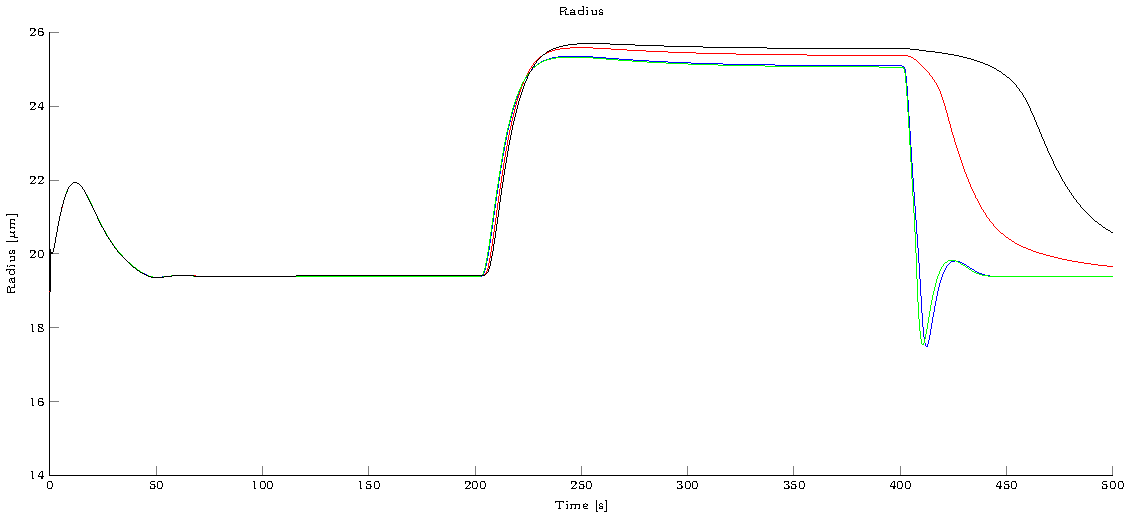
\includegraphics{figures/BK_rad_NVU14.pdf}
			\caption{Radius change for different BK-channel regulations}
			\label{fig:SMCfluxes}
		\end{figure}
\end{landscape}

%\end{document}

\section{Release notes}

\subsection{Changes to the previous version}

	\subsubsection{Astrocytic Calcium}
	
	\citet{Farr2011} implemented an NVU model based on a simple glutamate efflux into the SC simulating neuronal activity. This model included AC $Ca^{2+}$ variations induced by glutamate production into the SC and the subsequent efflux of $K^+$ into the PVS from a $Ca^{2+}$ mediated BK channel. In NVU 1.1 this BK channel was not \ca mediated and instead approximated by assuming a constant astrocytic \ca concentration.
			
	Although the model provided a qualitative description of neurovascular coupling the rate of change of $K_p$ was slow and the dilation of the associated arteriole took too long to reach even small dilations. The $K_p$ at which $v_i$ was maximally hyperpolarised was too high. 
	Therefore NVU version 1.1 did not contain any astrocytic $Ca^{2+}$ or glutamate input as the results were not satisfactory. 
	However various changes were implemented into the model and can be incorporated alongside the NO pathway, producing NVU version 1.2. 
	
	These changes included small fixes to the equations of the model by Michelle (e.g. changing a positive to a negative sign). 
	The additional state variables detailing the AC $Ca^{2+}$ model component are found in Table \ref{tab:NVU12ac}.
	
			\begin{table}[h!]
				\small
				\centering
					\begin{tabular}{c c l}
				\hline
				Variable & Unit & Description \\
				\hline
				$c_k$ & $\mu M$ & AC cytosolic $Ca^{2+}$ concentration \\
				$s_k$ & $\mu M$ & AC $Ca^{2+}$ concentration in the ER \\
				$h_k$ & - & inactivation variable denoting the action of $IP_3R$ that have not been activated by $Ca^{2+}$ \\
				$i_k$ & $\mu M$ & AC $IP_3$ concentration \\
				$eet_k$ &  $\mu M$ & $Ca^{2+}$ dependent EET production \\
				\hline
					\end{tabular}
					\caption{State variables related to $Ca^{2+}$ in the astrocyte}
					\label{tab:NVU12ac}
			\end{table}
			
	The ODE for astrocytic \ca is:
	\begin{equation}
	mklfmf
	\end{equation}
	
	\subsubsection{TRPV4 channel}
	
	Included is a transient receptor potential cation (TRPV4) channel on the astrocytic endfeet adjacent to the PVS.
	These channels are an important factor in astrocytic sensory and vasoregulatory functions as \cite{Dunn2013} have shown that certain TRPV4 channels can induce CICR in the endfeet of astrocytes and increase the strength of neurovascular coupling.
	The flux of $Ca^{2+}$ through the TRPV4 channel is based on the bidirectional model of \cite{Witthoft2012}.
	In this model vessel dilation activates the TRPV4 channels, allowing an influx of $Ca^{2+}$ from the PVS into the astrocytic cytosol. 
	The two additional state variables to the model are
	$m_k$: the open probability of the TRPV4 channel, and $c_p$: PVS $Ca^{2+}$ concentration (see Table \ref{tab:NVU12trpv4}).
			
					\begin{table}[h!]
						\small
						\centering
							\begin{tabular}{c c l}
						\hline
						Variable & Unit & Description \\
						\hline
						$c_p$ &  $\mu M$ & PVS $Ca^{2+}$  concentration (not in \cite{Farr2011}) \\
						$m_k$ & - & open probability of TRPV4 channel (not in \cite{Farr2011}) \\
						\hline
							\end{tabular}
							\caption{State variables related to the TRPV4 channel.}
							\label{tab:NVU12trpv4}
					\end{table}
					
			The ODE for the PVS \ca concentration is
				\begin{equation}
				\frac{d c_p}{dt} = - \frac{J_{TRPV_k}}{VR_{pa}} + \frac{J_{VOCC_k}}{VR_{ps}} - Ca_{decay_k} ( c_p - Ca_{min_k} ).
				\end{equation}
			
			Here $c_p$ always decays to the steady state value $Ca_{min_p}$ and $J_{VOCC_k}$ is a voltage operated calcium channel (VOCC) connecting the SMC to the PVS. When the membrane of the SMC hyperpolarises the channel closes. 
					
			The flux of \ca through the TRPV4 channel is:
				\begin{equation}
				J_{TRPV_k} = -\frac{1}{2} \frac{ G_{TRPV_k} m_k (v_k - E_{TRPV_k}) C_{correction} }{C_{astr_k} \gamma_k}
				\end{equation}
			
			The factor $1/2$ is there because there are 2 positive charges for every \ca ion \citep{Witthoft2013a}. 
			$E_{TRPV_k}$ is the Nernst potential of the TRPV4 channel:
				\begin{equation}
				E_{TRPV_k} = \frac{RT}{z_{Ca} F} \log \left(\frac{c_p}{c_k} \right).
				\end{equation}
			\\	
					
			The ODE for the open probability of TRPV4 channels is
				\begin{equation}
				\frac{d m_k}{dt} = \frac{m_{\infty_k} - m_k}{t_{TRPV_k}}.
				\end{equation}
						
			The equilibrium state of the TRPV4 channel is:
				\begin{equation}
				m_{\infty_k} = \frac{1}{1+\exp \left( {-\frac{\eta - epshalf_k}{\kappa_k}} \right) } 
								\frac{1}{1 + H_{Ca_k}} \left( H_{Ca_k} + \tanh \left( \frac{v_k - v_{1,TRPV}}{v_{2,TRPV}} \right) \right), 
				\end{equation}
			
			where $H_{Ca_k}$ is an inhibitory term:
				\begin{equation}
				H_{Ca_k} = \frac{c_k}{\gamma_{Cai}} + \frac{c_p}{\gamma_{Cae}},
				\end{equation}
			
			and $\eta$ is the local radial strain on the arteriole:
				\begin{equation}
				\eta = \frac{R - R_{passive}}{R_{passive}}.
				\end{equation}
			
			The strain on the perivascular endfoot of the AC is approximately equal to local radial strain on the arteriole since the endfoot surrounds the arteriole.	
			\\
				
			The flux of \ca through the TRPV4 channel is added to the AC \ca equation:
				\begin{equation}
				\frac{d c_k}{dt} = B_{cyt} \left( J_{IP3_k} - J_{pump} + J_{ER_{leak}} + \frac{\bm{{J_{TRPV_k}}}}{r_{buff}} \right). 
				\end{equation}
			
			The membrane potential of the AC is modified to include the TRPV4 channel:
				\begin{equation}
				\centering
				\scriptsize{
				v_k = \frac{g_{Na_k} E_{Na_k} + g_{K_k} E_{K_k} + \bm{g_{TRPV_k} m_k E_{TRPV_k}} + 
				                g_{Cl_k} E_{Cl_k} + g_{NBC_k} E_{NBC_k} + 		                g_{BK_k} w_k E_{BK_k} - 
				                J_{NaK_k} F / C_{correction}}{ g_{Na_k} + g_{K_k} + g_{Cl_k} + g_{NBC_k} + \bm{ g_{TRPV_k} m_k } + g_{BK_k} w_k }.
				           }
				\end{equation}
			
			The conductance $g_{TRPV_k}$ is calculated using the area of the astrocytic endfeet (similar to the calculation of the conductance of the BK channel at the astrocytic endfeet):
				\begin{equation}
				g_{TRPV_k} = \frac{G_{TRPV_k} 10^{-12}}{A_{ef_k}},
				\end{equation}
			
			where the conductance is multiplied by $10^{-12}$ to convert from $pS$ to $\Omega^{-1}$ (mho).
			
			The new parameters are found in Table \ref{tab:NVU12trpv4param}. 
			
			\begin{table}[h!]
				\small
				\centering
					\begin{tabular}{c c c l}
				\hline
				Parameter & Value & Unit & Description \\
				\hline
				$Ca_{decay_k}$ & 0.5 & - & Rate of decay of \ca in PVS \\
				$Ca_{min_k}$ & 2000 & $\mu$M & steady state value of \ca in PVS \\
				$t_{TRPV_k}$ & 0.9 & mV & Decay rate of the open probability $m_k$ \\
				$G_{TRPV_k}$ & 50 & pS & Conductance of TRPV4 channel \\
				$C_{correction}$ & $10^3$ & - & Convert from V to mV \\
				$C_{astr_k}$ & 40 & pF & AC cell capacitance \\
				$\gamma_k$ & 834.3 & mV $\mu M^{-1}$ & scaling factor relating movement of ions to membrane potential \\
				$epshalf_k$ & 0.1 & - & Strain required for half activation of the TRPV4 channel \\
				$\kappa_k$ & 0.1 & - & Related to strain and TRPV4 channel \\
				$v_{1,TRPV}$ & 0.12 & mV & Related to voltage gating of TRPV4 channel \\
				$v_{2,TRPV}$ & 0.013 & mV & Related to voltage gating of TRPV4 channel \\
				$\gamma_{Cai}$ & 0.01 & $\mu$M & Related to \ca concentration \\
				$\gamma_{Cae}$ & 200 & $\mu$M & Related to \ca concentration \\
				$r_{buff}$ & 0.05 & - & Rate of \ca buffering at the endfoot compared to the astrocyte body \\
				\hline
					\end{tabular}
					\caption{Model parameters related to the TRPV4 channel.}
					\label{tab:NVU12trpv4param}
			\end{table}
			
			Note that the flux of \ca through the TRPV4 channel is buffered at a lower rate $r_{buff}$, as the channel is located at the astrocytic endfoot and buffering is described by \cite{Witthoft2013} in the astrocytic soma. Therefore it is reasonable to assuming buffering at the smaller endfoot of the astrocyte will be at a lower rate. 
	
	\subsubsection{Nitric Oxide}
	
		Nitric oxide (NO) is a neurotransmitter known to act as a potent cerebral vasodilator. It is not produced in advance or stored and due its small size it is able to diffuse widely and readily in all 3 dimensions and is not limited to local effects, setting it apart from other signalling molecules of the central nervous system. It can rapidly spread even through membranes as it is extremely diffusible in aqueous and lipid environments. However NO has a very short half life as it is an unstable gaseous free radical, limiting its activity temporally \citep{Dobutovic2011} . 
					
		NO is produced in a variety of different tissues. The biochemical reaction that synthesises NO is catalysed by the enzyme family of nitric oxide synthases (NOS): neuronal (nNOS), endothelial (eNOS), and inducible (iNOS), found in neurons, ECs and multiple cell types respectively \citep{Forstermann2006}. 
		The literature suggests that the production source and quantity of NO determines its function; NO may either act neuroprotectively by controlling vascular smooth muscle tone and blood flow and hence preventing ischaemic cell injury, or neurotoxically leading to cerebral degeneration \citep{aurelia2010role}.
				
		The focus of the NO pathway is on NO production by nNOS and eNOS. Both enzymes' activation is mediated by intracellular $Ca^{2+}$ of the NE and EC respectively and eNOS is also activated by blood flow induced wall shear stress (WSS) in cerebral arterioles.
		NO is able to diffuse rapidly into other compartments. When NO reaches the SMC it interacts with intracellular enzyme activation and regulates SMC relaxation. 
		The dynamics of NO in the NE, AC, SMC and EC are described by using mass balance formulations. The NO concentration in compartment $j$ is:
			\begin{equation}
			\frac{d[NO]_j}{dt} = p_{NO,j} - c_{NO,j} + d_{NO,j}.
			\end{equation}
		$ p_{NO,j}$ is the production flux,  $c_{NO,j}$ is the consumption flux (i.e. reaction with oxygen or other molecules), and $d_{NO,j}$ is the diffusive flux. Diffusion is assumed to be linear with characteristic distance of $\Delta x = 3.75 \; \mu$m between the EC and SMC layers, and  $\Delta x = 50 \; \mu$m between the NE and SMC layers.
		The production rate is dependent on the concentration of activated NOS. nNOS and eNOS are thought to be the most influential NO producers, hence we assume NO production in only the NE and EC compartments and no production in the other cell types.
		
		NO synthesis in the NE is catalysed by nNOS in response to glutamate induced calcium influx into the post synaptic neuron and depends on the available concentration of the biochemical substrate L-Arginine (L-Arg) and oxygen ($O_2$). The nNOS activation is triggered by glutamate in response to neuronal activation. 
		NO production in the EC is catalysed by eNOS dependent on the availability of L-Arg and $O_2$ and is mediated by WSS. 
	
		NO, via its second messenger cGMP, influences the contraction of the SMC ($AMp$, $Mp$, $AM$, $M$) and the open probability of the SMC \pot channel $w_i$. NO activates soluble guanylyl cyclase (sGC) which catalyses the formation of cGMP. cGMP changes the rate constants $K_2$ and $K_5$ for the dephosphorylation of $Mp$ to $M$ and $AMp$ to $AM$ (these rate constant were previously set at $0.5 \; s^{-1}$ based on \citet{Koenigsberger2006}). $w_i$ is shifted to the left by cGMP via the equilibrium state $K_{act_i} (c_{w,i})$ with $c_{w,i}$ as a function of cGMP.
		\\
		
		The initial NVU model version 1.1 is extended into version 1.2 by additional mathematical equations that represent production, diffusion and consumption of NO in different cell types, as well as the interaction of NO with other biochemical species and ion channel open probabilities. The model of NVU 1.2 also contains astrocytic $Ca^{2+}$ and a TRPV4 channel. 		
		The additional NO pathway equations are found in the appendix of \cite{Dormanns2016} and corresponding additional state variables are detailed in Table \ref{tab:NVU12}. 		
		\todo[inline]{add equations here}

		\begin{table}[h!]
			\small
			\centering
				\begin{tabular}{c c l}
			\hline
			Variable & Unit & Description \\
			\hline
			$NO_n$ & $\mu M$ & NE NO concentration \\
			$NO_k$ & $\mu M$ & AC NO concentration \\
			$NO_i$ & $\mu M$ & SMC NO concentration \\
			$NO_j$ & $\mu M$ & EC NO concentration \\
			$cGMP$ & $\mu M$ & SMC cGMP concentration \\
			$eNOS$ & $\mu M$ & activated eNOS \\
			$nNOS$ & $\mu M$ & activated nNOS \\
			$c_n$ & $\mu M$ & NE cytosolic $Ca^{2+}$ concentration \\
			$E_b$ & - & fraction of sGC in the basal state \\
			$E_{6c}$ & - & fraction of sGC in the intermediate form \\
			\hline
				\end{tabular}
				\caption{State variables related to the NO pathway}
				\label{tab:NVU12}
		\end{table}
		

		Neuronal stimulation is simulated by an input of both glutamate and $K^+$ into the SC. The implementation of the NO pathway results in a larger steady state vessel radius, due to a constant supply of vasodilatory NO from the EC and NE. The radius profile also shows a larger and longer response to stimulation. 
		The response of the radius to stimulation can be divided into two components: the fast component in response to the SC $K^+$ increase (modelled by NVU version 1.1) and the slow component only found with the addition of the NO pathway. 
		
		The slower component of the model with the NO signalling pathway is the increase of cGMP in the SMC. This leads to the shift of the open probability of the SMC $K^+$ channel $w_i$. The  efflux of $K^+$ from the PVS increases with the opening of the channel so that the PVS $K^+$ concentration drops at a faster rate. Instead of reaching steady state conditions after around 100 s, as the model would do if the NO pathway is not included (version 1.1), the SMC membrane potential $v_i$ drops further. Consequently the VOCC channel closes further and the SMC $Ca^{2+}$ concentration decreases. As an overall behaviour the vessel dilates further and returns back to the resting state more slowly. 
		
		Hence the SC $K^+$ release governs the fast onset of vasodilation whilst the NO-modulated mechanisms (increase of SMC cGMP leads to shift in $w_i$) and the WSS activated NO release from the EC is responsible for maintaining the dilation longer and thus providing more oxygen and glucose to adjacent brain tissue with increased cerebral blood flow. In the resting state the EC provides the major contribution towards vasorelaxation, whereas during neuronal stimulation NO produced by the NE dominates \citep{Dormanns2016}.	
		
		The radius $r$ in this term is set as constant 25 $\mu m$ in order to create a reasonable boundary condition at the lumen side of the NVU based on physiological results.
		

%\section{Summary}

\subsection{Conclusions Current Model}
The Neurovascular coupling (NVC) matlab code version 0.1 is able to describe the relationship between a neural input signal into the \gls{SC} and the dilation or constriction of the bloodvessel. \\

An input signal (neuronal \gls{K} pulse) is taken up by the astrocyte, which repolarize its cell membrane. This repolarization results in a efflux of \gls{K} of the astrocyte in the PVS. This increase in \gls{K} in de PVS causes the opening of the KIR channel in the SMC and to extrude more \gls{K} in the PVS. This hyperpolarization closes the voltage operated calcium channels (VOCC), preventing the influx of \gls{Ca}. The decreased cytosolic \gls{Ca} in the SMC then causes dilation of the blood vessel.\\




\subsection{Further Work} \label{sec:furtherwork}

There are several pathways which have to be included in order to complete and extend the existing model. These pathways are listed below:
\begin{itemize}
\item A MATLAB model of the AA and 20-HETE pathway which has been developed needs to be included in the model. This model also includes the \gls{Ca} dynamics in the AC and therefore is an important contribution to the existing model
\item The NO (Nitric oxide) model needs to be included in this model
\item A general pH model needs to be included for the SMC and later on also the Astrocyte and EC.
\item And also the AA \& 20-HETE model needs to be included
\end{itemize}


\subsection*{Acknowledgement}
May thanks to Christine French, who helped transfer our chaotic sentences into readable English! 

%At the moment the epoxyeicosatrienoic acid (EET) and the arachidonic acid (AA) pathway are not included in the astrocyte model.\\
%\documentclass[12pt]{article}
\usepackage{amsmath,xcolor,todonotes,graphicx,marvosym,natbib,dsfont,import,hyperref}

\begin{document}


\section{Envy-You Version 1.0}
This most recent version 1.0 of the envy-you code is based on the previous versions envy-you 0.1 and 0.2, the main changes being:

\subsection{Parameters}
The most important parameters that can be used to adjust the model are listed as global variables in the main script 'NVC\_main.m', namely
\begin{itemize}
	\item [\textit{t\_start} -] start time of simulation (s)
	\item [\textit{t\_end} -]  end time of simulation (s)
	\item [\textit{startpulse} -]  start of neuronal pulse (s)
	\item [\textit{lengthpulse} -]  length of neuronal pulse (s)
	\item [\textit{CASE} -]  set of coupling coefficients 
	\item [\textit{J\_PLC} -]  EC agonist concentration ($\mu$M s$^{-1}$)
	\item [\textit{C\_Hillmann} -]  scaling factor for the Hai\&Murphy rate constants based on \citet{Hillman2011}
	\item [\textit{stretch\_ch} -] to activate/deactivate stretch-activated channels in EC and SMC
	\item [\textit{only\_Koenig} -]  to simulate only the Koenigsberger model (other sub-models will still be considered, but the KIR channel is set to 0)
\end{itemize}
At the end of each simulation \textit{save\_all()} is called and will give the option to save all parameters and figures in a separate folder with a time stamp. 

\subsection{Radius and wall thickness equation}
The previous equations of the radius, R, and the arterial wall thickness, \textit{h}, seemed to have led to an instability of the system at very low $J_{plc}$ values. Due to that h is now set to a fixed ratio of the radius (see 'all\_fluxes.m'):
\[h = 0.1R\]
\subsection{Hillmann coefficients}
The reaction rate constants used by \citep{Hai1988} are based on experiments with swine carotid arteries and there is no evidence that they can be used for human brain arteries. Within her paper \citep{Hillman2011} E. Hillman's  could show that the hemodynamic response in rats takes place within a couple seconds, whereas with the \citep{Hai1988} model we obtain maximal dilation within approximately a minute. Based on \citep{Hillman2011} we introduce a scaling coefficient \textit{'C\_Hillmann'}, that allows us to scale all rate constants simultaneously. 

\subsection{Figures position} 
All figures are now automatically placed in the main screen. 

\subsection{Coupling coefficients}
The three coupling coefficients ($v_{cpl}, Ca_{cpl}, P3_{cpl}$) are chosen the following:

\begin{table}[h!]
\centering
\caption{All CASE's.}
\begin{tabular}{c c c c}
\hline
       & $v_{cpl}$ (s$^{-1}$) & $Ca_{cpl}$ (s$^{-1}$)& $P3_{cpl}$ (s$^{-1}$)\\
       \hline \hline
CASE 0 & 0     & 0     & 0     \\
CASE 1 & 0.5   & 0     & 0.05  \\
CASE 2 & 0.5   & 0.05  & 0.05  \\
CASE 3 & 0     & 0     & 0.05  \\
CASE 4 & 0.5   & 0.05  & 0     \\
CASE 5 & 0.5   & 0     & 0     \\
CASE 6 & 0     & 0.05  & 0     \\
CASE 7 & 0     & 0.05  & 0.05  \\
\hline
\end{tabular}
\end{table}

\subsection{Corrected mistakes}
\begin{itemize}
\item plotting of stretch-activated channels in EC (figure 3 - EC fluxes)
\item K$_{7}$ corrected to be K$_{4}$ in the differential equation for AMp (didn't change any results because K$_{4}$ = K$_{7}$ = 0.1 s$ ^{-1} $)
\item \textit{v\_Ca2} changed back to -24 mV (original value from \cite{Koenigsberger2005})
\item maximal voltage coupling $v_{cpl}$ set to 0.5 s$^{-1}$ (any stronger coupling leads to EC clinging to SMC and a too low membrane potential in SMC for VOCC to open during neuronal pulse)
\end{itemize}


\bibliography{library} 
\bibliographystyle{KathisBibstyle} 

\end{document}

%\nocite{*} % a good, but also very dangerous command! :) Shows all library entries

\bibliography{library2} %library.bib - any library file - either generated by Mendeley, Qiqqa, JabRef ... or write it your own, but don't complain if you choose to do so! :)
\bibliographystyle{KathisBibstyle} % default: plain, ieeetr, named, acm, but there are many hp's where you can autogenerate your own Bibstyle! - or use mine for the start :)

\newpage
%\deftranslation[to=German]{Acronyms}{Abkürzungsverzeichnis}
%\printglossary[type=\acronymtype,style=long]
\printglossary[style=altlist,title=Glossary] %Print the glossary
%\printglossary[type=\acronymtype,style=long] %Print list of acronyms

%\section{MATLAB Code}

\subsection*{NVC\_main.m}
    \lstinputlisting[language=Matlab]{NVC_main.m}
\newpage
\subsection*{DEsyst.m}
    \lstinputlisting[language=Matlab]{DEsyst.m}
\newpage
\subsection*{all\_fluxes.m}
    \lstinputlisting[language=Matlab]{all_fluxes.m}
\newpage
\subsection*{writeFlux.m}
    \lstinputlisting[language=Matlab]{writeFlux.m}
\newpage
\subsection*{InitCond.m}
    \lstinputlisting[language=Matlab]{InitCond.m}
\newpage
\subsection*{all\_indices.m}
    \lstinputlisting[language=Matlab]{all_indices.m}
\newpage
\subsection*{all\_constants.m}
    \lstinputlisting[language=Matlab]{all_constants.m}
\newpage
\subsection*{createPulse.m}
    \lstinputlisting[language=Matlab]{createPulse.m}
\newpage
\subsection*{createSig.m}
    \lstinputlisting[language=Matlab]{createSig.m}
\newpage
\subsection*{getRef.m}
    \lstinputlisting[language=Matlab]{getRef.m}
\newpage
\subsection*{plot\_all.m}
    \lstinputlisting[language=Matlab]{plot_all.m}
\end{document}